%% Dissertationsvorlage
%%
%% Karlsruhe Institute of Technology
%% Institute for Program Structures and Data Organization
%% Chair for Software Design and Quality (SDQ)
%%
%% Dr.-Ing. Erik Burger
%% burger@kit.edu
%%
%% Siehe https://sdqweb.ipd.kit.edu/wiki/Dokumentvorlagen
%%
%% {$HeadURL: https://svnserver.informatik.kit.edu/i43/svn/presentations/SDQ-Dissertations-Vorlage/LaTeX-Dateien/sdqdiss.tex $}
%% {$LastChangedDate: 2018-08-02 14:23:11 +0200 (Do, 02 Aug 2018) $}
%% {$LastChangedRevision: 1078 $}
%% {$LastChangedBy: burger $}

%% Dokumentoptionen
%
% Für das Proposal bzw. vorgelegte Fassung (DIN A4):
%
% \documentclass{sdqdiss-a4}
%
% Für die Druckfassung im Format von KIT Scientific Publishing (DIN A5)
% bitte auch für die Bindekorrektur den Umfang des Dokuments eintragen:
%
% z.B. \documentclass[largediss]{sdqdiss-a5-ksp}
% 
% +------------+-----------------------+
% | Seitenzahl | Option                |
% +------------+-----------------------+
% | < 200      | smalldiss             |
% | 200–399    | mediumdiss (Standard) |
% | > 400      | largediss             |
% +------------+-----------------------+

\documentclass[fleqn % left-aligned formula, passed to loading of amsmath
]{sdqdiss-a5-ksp}%24x17-ksp} %5-ksp}

% Benötigt für die Typewriter-Schriftart
\usepackage[T1]{fontenc}
\usepackage[utf8]{inputenc}
  
% Für Sprachumschaltung
\usepackage[ngerman,english]{babel}

\usepackage{templates/complete_template}

%%% TOGGLES
\newtoggle{showCopiedFrom}
\toggletrue{showCopiedFrom}

% Abstract
\newcommand{\Abstract}[1][Abstract]{\chapter*{#1}\addcontentsline{toc}{chapter}{#1}\markboth{#1}{#1}} 


%%
%% Beginn des Dokuments
%%

%\title{Preserving Consistency of Multiple Model with Networks of Transformations}
\title{Building Transformation Networks for Consistent Evolution\\ of Multiple Models}
%\title{Transformation Networks for Consistent Evolution of Multiple Heterogeneous Models}
\author{Heiko Klare}
\subject{}

\subtitle{
\vskip2em
zur Erlangung des akademischen Grades eines\\[1em]
{\Large Doktors der Ingenieurwissenschaften}\\[1em]
%{\Large Doktors der Naturwissenschaften}\\[1em]
der KIT-Fakultät für Informatik\\
des Karlsruher Instituts für Technologie (KIT)\\[.5em]
{vorgelegte}\\[.3em]
{\Large Dissertation}
}

\author{\normalsize{von}\\
{\LARGE Heiko Klare}\\
\normalsize{aus Höxter}
}

\publishers{%
\flushleft\small
Tag der mündlichen Prüfung: XX. Monat XXXX\\
Erster Gutachter: Prof.\ Dr.\ Ralf H.\ Reussner\\
Zweiter Gutachter: Prof.\ Dr.\ Colin Atkinson\\
}

\date{}

\includeonly{
    sections/1_prologue/110_introduction,
    sections/1_prologue/120_foundations,
    sections/2_properties/220_levels,
    sections/3_correctness/3100_correctness,
    sections/3_correctness/3200_compatibility,
    sections/3_correctness/3300_synchronization,
    sections/3_correctness/3400_orchestration,
    sections/3_correctness/3500_errors,
    sections/3_correctness/3600_evaluation,
    sections/4_quality/610_topologies,
    sections/4_quality/620_improvement,
    sections/4_quality/630_language,
    sections/4_quality/640_integration,
    sections/4_quality/650_evaluation,
    sections/9_epilogue/910_relatedwork,
    sections/9_epilogue/920_futurework,
    sections/9_epilogue/930_conclusions
}

%%
%% Titelseite
%%

\begin{document}
\maketitle

%%
%% Abstract/Zusammenfassung
%%
% start with roman page numbers
\frontmatter

%% Englischer Abstract
\selectlanguage{english}
\Abstract{}
%\Blindtext[10]

%% Deutsche Zusammenfassung
\selectlanguage{ngerman}
\Abstract[Zusammenfassung]{}
%\Blindtext[10]

% Sprachumschaltung
\selectlanguage{english}

%%
%% Inhaltsverzeichnis
%%
\begingroup
\setlength\cftbeforepartskip{4pt}  % change space before part
\setlength\cftbeforechapskip{-5pt}   % change space before chapter
% Same indent for part and chapter, like in KSP template
\renewcommand\cftpartnumwidth{1.5em}
\shorttoc{Contents Overview}{0}
\endgroup

\cleardoublepage
\setcounter{tocdepth}{2}
\tableofcontents

% Linksbündige Einträge ohne Einzug
\selecttocstyleoption{tocflat}
\cleardoublepage
\listoffigures
\cleardoublepage
\listoftables

%%
%% Inhalt
%%
% restart with arabic page numbers
\mainmatter

%% TODO: Remove of not necessary anoymore
%\def\clearpage{\vspace{1em}}
%\def\cleardoublepage{\vspace{1em}}
%\def\newpage{\vspace{1em}}
%\def\pagebreak{\vspace{1em}}

\part{Prologue
	\pgsize{35 p.}
}

\chapter{Introduction
    \pgsize{25 p.}
}
\label{chap:introduction}

\mnote{High-level thesis summary}
In this thesis, we discuss how multiple artifacts used to develop a software or software-intensive system can be kept consistent by combining transformations between their specification languages.
We research how multiple transformations, which specify consistency and its preservation, can be developed \emph{independently}, such that their combination operates \emph{correctly} and such that they can be reused \emph{modularly}.

\mnote{Introduction outline}
In the following sections, we first introduce the context of preserving consistency between multiple artifacts and identify existing challenges. We then derive two problem statements from these challenges and define a research goal and fine grained questions, as well as according contributions that counter these challenges.
Finally, we give an overview of the structure of this thesis and give guidelines how to read it.


%%
%% MOTIVATION
%%
\section{Consistency of Multiple Models}

\mnote{Increasing system complexity}
Engineers develop software and software-intensive technical systems of ever increasing scale.
This leads to a continual increase in complexity of the artifacts used to describe such systems~\cite{murer2011evolution}.
As a direct consequence of the increasing system sizes, engineers inevitably have to deal with their inherent essential complexity.
Various tools support the development process by reducing the accidental complexity to allow engineers to focus on handling the essential complexity~\cite{brooks1987NoSilverBullet-Computer, fraser2008NoSilverBulletReloaded-Software}.

\subsection{Consistency in System Engineering}

\mnote{Fragmented information to deal with essential complexity}
To better handle the essential complexity of a system, engineers usually use multiple tools to describe and analyze different parts or properties of a system under development in different artifacts.
In the following, we denote all these artifacts as \emph{models}, according to the notion of \citeauthor{bezivin2005sosym} that \enquote{everything is a model}~\cite{bezivin2005sosym}.
This reduces the information to deal with to what is relevant for the development task of each person's role.
In classical engineering disciplines like construction, mechanical and electrical engineering, this has been common practice for a long time and is often called \emph{\gls{MBSE}}~\cite{estefan2007MbseSurvey}.
For example, the development of software for \glspl{ECU} in automobiles comprises different tools or standards for specifying the system and software architecture, such as SysML~\cite{sysml} or AUTOSAR~\cite{scheid2015autosar}, for defining the behavior, such as MATLAB/Simulink~\cite{simulink} or ASCET~\cite{ascet}, and for defining the deployment on multi-core hardware architectures, such as Amalthea~\cite{amalthea, wolff2014a}.
In software engineering, such a development methodology is also getting growing attention.
It is often referred to as \emph{\gls{MDSD}}~\cite{stahl2006a}.
Such a development process foresees other artifacts beyond code as primary artifacts to describe the system under construction.
While code only specifies the functionality of a system, other tools can be used, for example, to define the software architecture and its deployment, such as the \gls{UML}~\cite{uml}, analyzing and predicting the software performance, such as the Palladio Simulator~\cite{reussner2016a}, and for specifying the requirements, like IBM Rational Doors~\cite{laplante2012RequirementsEngineering-Book}.

\mnote{Accidental complexity due to information fragmentation}
While this \emph{fragmentation} of information across models developed with different tools eases dealing with the essential complexity of a system, it increases accidental complexity.
Since all these models describe the same system, they usually share an overlap of information in terms of implicit \emph{dependencies} or \emph{redundancies}.
If modifications of overlapping information are not propagated properly across all dependencies and redundancies, \emph{inconsistencies} can occur.
For example, requirements changes have to be reflected in the software architecture and implementation, and modifications of the software architecture have to be reflected in the code.
Since systems are usually developed iteratively and incrementally, there is no strict direction in which changes have to be propagated to preserve consistency, but in general any model can be changed and require updates of others.

\mnote{Consistency of fragmented information}
The overlaps of information, for example in the above mentioned tools for \gls{ECU} software development~\cite{giese2010a}, are often not documented explicitly~\cite{mazkatli2017ase}, but only known by engineers.
Performing the task of updating overlapping information manually is, however, time-consuming and error-prone.
The automation of checking and of preserving consistency of information is still poorly supported in current development processes for large systems, as a recent survey has shown \owncite{guissouma2018study}.
But automating that process is necessary to reduce the accidental complexity induced by the fragmentation of information across multiple models.

\mnote{Transformations for binary consistency} %State of research: transformations to preserve consistency}
A common approach to automate the process of checking and preserving consistency of models are \emph{incremental model transformations}.
%If models shall or cannot be generated anew after each change, especially \emph{incremental} transformations are of interest.
Tools describe their models in specific languages, for example denoted by \gls{XML} schemes or \glspl{DSL}.
A transformation specifies how models of one or more of such languages have to be updated after engineers make changes to a model of another language.
The subclass of \emph{bidirectional} model transformations~\cite{stevens2010sosym}, which specify the relations between two models and routines how consistency of their instances can be restored after changes in any of them, is particularly well researched.
System development usually involves more than two tools and thus models of more than two languages to be kept consistent.
The use of transformations to check and preserve consistency between more than two models is, however, less researched~\cite{stevens2020BidirectionalTransformationLarge-SoSym}.
It gained recent attention in a dedicated Dagstuhl seminar~\cite{cleve2019dagstuhl}.


\subsection{Distributed and Reusable Consistency Knowledge} %Modular and Independent Consistency Specification}

\mnote{Multidirectional transformations vs. networks}
Two general approaches for consistency of multiple %, especially more than two, 
models by means of transformations are using a \emph{multidirectional} transformation or a combination of multiple bidirectional (or multidirectional) transformations to networks of them.
A single multidirectional transformation is beneficial from a theoretical perspective, because it is not prone to contradictions between the transformations to be combined and it provides higher expressiveness~\cite{stevens2020BidirectionalTransformationLarge-SoSym}.
For practical application, however, multidirectional transformations suffer from missing modularity, as they require a single person or team to define the overall relations between all languages.
Additionally, it is difficult to think about complex multiary relations between models of multiple languages~\cite{stevens2020BidirectionalTransformationLarge-SoSym} and, even worse, the knowledge required to define such a relation may not even exist~\owncite{klare2018docsym}.

\begin{figure}
    \centering
    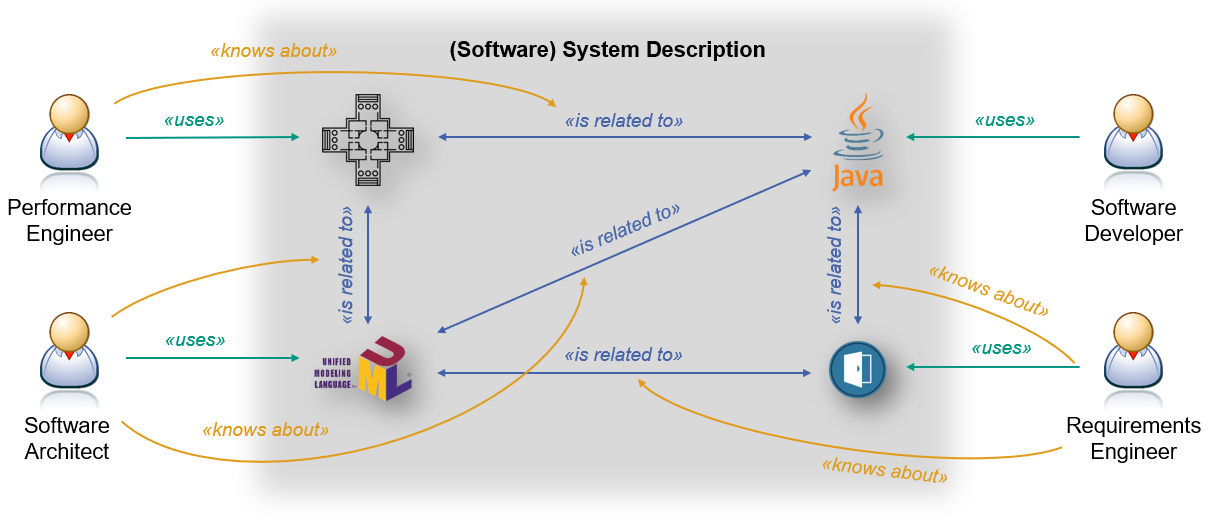
\includegraphics[width=\textwidth]{figures/prologue/introduction/distributed_knowledge.png}
    \caption[Tools and distributed knowledge in engineering processes]{Different tools and roles involved in an exemplary software development process and distributed knowledge about the relations between models of the different tools.}
    \label{fig:introduction:distributed_knowledge}
\end{figure}

\mnote{Distributed knowledge about consistency}
Domain experts deal with the tools and corresponding models they require for their tasks in developing a system.
Usually, each of them is only concerned with a subset of all tools involved in the development of a system.
For example, a performance engineer may be concerned with an instance of the \gls{PCM}, which represents a component-based architecture description of the system, to perform an architecture-based prediction of the system's performance and knows how this description is reflected in the system implementation in Java.
A software architect may use \gls{UML} models for the architecture specification and know how they are related to the implementation as well as to the component-based architecture models in \gls{PCM}.
Finally, a requirements engineer may use IBM Rational Doors and know how they have to be reflected in the architecture specification and implementation to consider the models consistent.
These exemplary relations are depicted in \autoref{fig:introduction:distributed_knowledge}.
No matter whether this is how knowledge is actually present at the different roles in a concrete scenario, it emphasizes that knowledge about the relations between languages and their models will usually be distributed across different experts as soon as multiple models are involved.
In large software systems, a single developer cannot know about all model dependencies~\cite{petrenko2008a}.
In consequence, a process for specifying consistency by means of transformations has to support a kind of \emph{modularity} to foster independent specification of distributed knowledge.
% Maybe discuss that not only binary is case if covered, but also modular multiary case

\mnote{Reuse of consistency specifications}
Furthermore, an automation especially proposes benefits if it is used often.
A specification of consistency and its preservation between common languages, such as \gls{UML} and a programming language like Java, can be reused across multiple projects.
Not each project will, however, use exactly the same tools.
Considering the example in \autoref{fig:introduction:distributed_knowledge}, if the relation between \gls{PCM} and Java was, at least partly, expressed indirectly across the relations between \gls{PCM} and \gls{UML} as well as \gls{UML} and Java, it would not be possible to reuse that specification in another project that only uses \gls{PCM} and Java but omits \gls{UML}.
Thus, parts of the consistency specifications, i.e., specifications for subsets of the tools in a project, should be reusable, comparable to \gls{COTS}.
In consequence, a process for specifying consistency by means of transformations has to support the \emph{independent} specification of \emph{modular} transformations, which can be combined with arbitrary other modular transformations in different contexts.

\mnote{Context assumptions}
To support the context induced by the previous considerations, we focus on combinations of transformations, be they bidirectional or multidirectional, instead of having only a single multidirectional transformation.
We call such a combination a \emph{transformation network}.
To summarize the previous considerations, we need to cover the following context assumptions to the specification of the individual transformations of a network:
\begin{properdescription}
    \item[Modularity:] Transformations are defined in a modular way, i.e., each transformation does only specify consistency and its preservation for a subset of the tools used in an actual development project.
    \item[Independence:] Transformations are defined independently, i.e., each transformation can be developed without considering the contents of the other transformations to be combined with.
\end{properdescription}


\subsection{Orchestration of Transformation Networks}
\label{chap:introduction:consistency:orchestration}

\mnote{Limitations of transformation orchestration}
Combining several modular and independently developed transformations requires their \emph{orchestration}, i.e., the decision in which order the transformations need to be executed to restore consistency.
Existing work proposes, for example, to define an execution order explicitly ~\cite{pilgrim2008a, vanhooff2007UniTI-MODELS} or to derive a kind of topological order~\cite{stevens2020BidirectionalTransformationLarge-SoSym}.
Such approaches either require a manual decision for the orchestration or restrict the execution to specific topologies, such as directed acyclic graphs or trees. %, which limits the kinds of supported transformation networks.
In any case, strong assumptions to the individual transformations or the topology of the supported networks are made.
%To foster distributed development and partial reuse, arbitrary topologies should be supported (Universality, Reusability).

\mnote{Universal combination of specifications}
It is yet unclear how arbitrary modular and independently developed transformations can be combined in a universal way.
%This especially concerns the role of the transformation developer.
It is neither known how a developer can achieve a \emph{correct} transformation network specification, i.e., transformations and an orchestration of them that delivers consistent models when applied, nor how he or she can systematically improve quality attributes of the network such as %\emph{reusability} and 
\emph{comprehensibility}.
%For the role of the transformation user, it is yet unknow how to support him in understanding the reasons whenever transformations fail to deliver consistent models.

%\mnote{Two roles: transformation users and developers}
%Fragmentation addresses challenges of transformations users.
%Challenges of developers yet addressed for binary case.

\begin{figure}
    \centering
    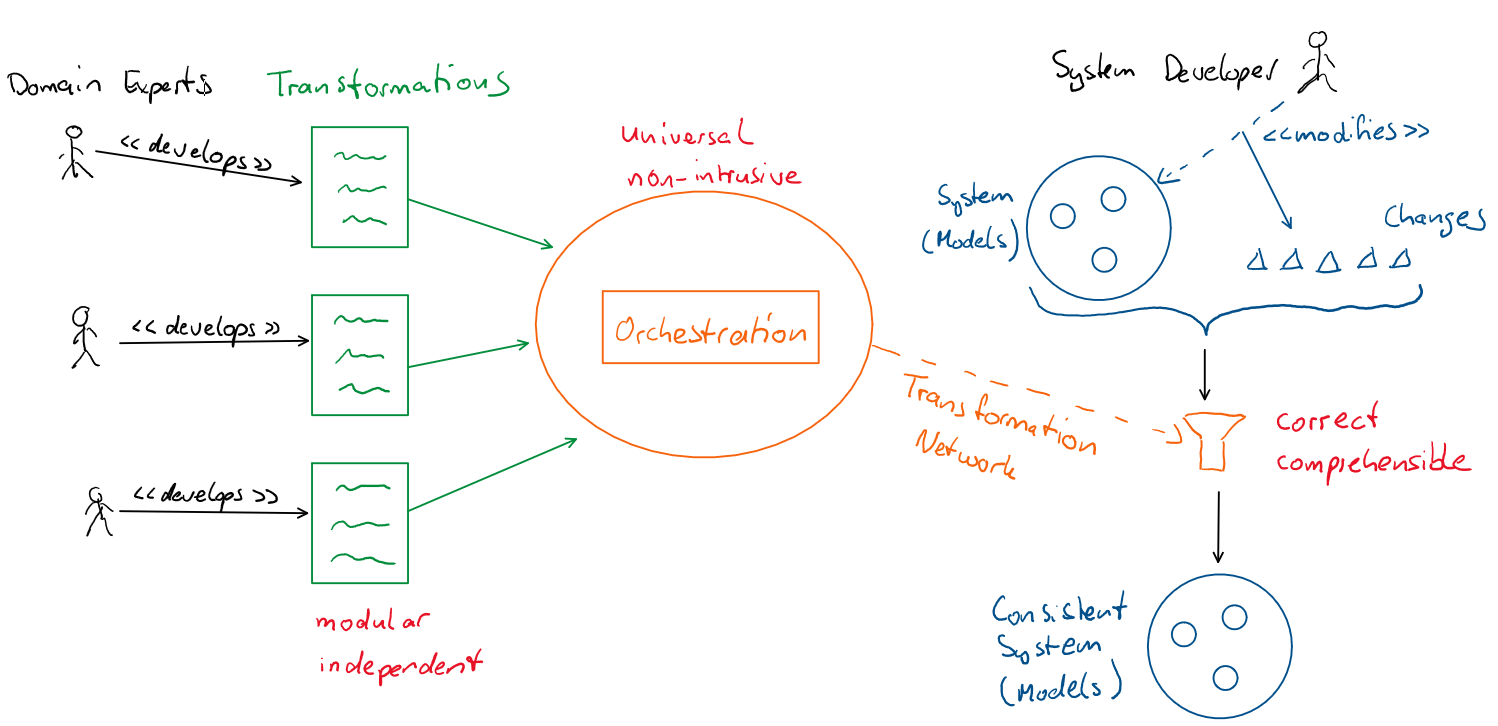
\includegraphics[width=\textwidth]{figures/prologue/introduction/overall_process.png}
    \caption[Process of specifying and executing a transformation network]{The process of specifying and executing a transformation network. 
    % Different domain experts specify transformations, which are combined to a transformation network by an orchestration mechanism that decides which transformations have to be executed in which order. If an actual system is developed and a developer modified models, the network is applied to these models and the performed changes to produce a consistent system description again. 
    Artifacts defined by transformation developers are marked green, artifacts at runtime are marked blue and the artifacts for orchestration and application developed in this thesis are marked orange. The assumed and envisioned properties are denoted in red.}
    \label{fig:introduction:process_overview}
\end{figure}

\mnote{Envisioned properties and process}
Under the assumption of a modular and independent specification of the individual transformation, we aim at an approach for executing transformation networks that has the following properties:
\begin{description}
    \item[Universality:] The approach shall be able to process transformation networks of arbitrary topology. In particular, specific topologies cannot be assumed or prescribed if the assumption of independent development shall be supported.
    \item[Non-intrusiveness:] The approach shall be non-intrusive. When independently developed transformations are combined to a network, they should be treated as black-boxes and there should be no need to adapt them to be used together.
    %It must be possible to combine arbitrary specifications. This means that the approach should not restrict which specifications can be combined, especially not which topology, induced by the specifications (such as only a tree) should be supported. In fact, requirements that all specifications have to fulfill may be defined, but apart from that the usability of one specification should not depend on the existence or non-existence of another.
    \item[Correctness:] The approach shall operate correctly. If it applies transformations to preserve consistency of models, the result must be consistent or indicate an error. The identification and definition of a more precise and appropriate notion of correctness is part of the contributions of this thesis.
    %\item[Reusability:] The approach shall improve reusability. This means that the individual transformations shall be reusable independently.
    \item[Comprehensibility:] The approach shall improve comprehensibility. If the transformations are not able to produce models that are actually consistent, it should support the user in finding the reason for that.
\end{description}
The envisioned process with the involved roles, artifacts and required properties is depicted in \autoref{fig:introduction:process_overview}.
Different domain experts specify transformations, which are combined to a network with an orchestration mechanism that decides in which order transformations have to be executed. If an actual system is developed and a system developer modifies models, the transformations of the network are applied to these models and the performed changes to produce a consistent system description again.

\mnote{Thesis contributions}
In this thesis, we contribute to support the process of building transformation networks that have the defined properties by providing a formal foundation for transformation networks of arbitrary topology and defining a formal notion of correctness for them.
We discuss how correctness of a universal approach to orchestrate and apply the transformations of a network can be achieved by construction or at least by analysis, and which properties the different involved artifacts, such as transformations and their orchestration, have to fulfill for that.
The proposed strategy to orchestrate transformations improves comprehensibility in cases when it is not able to execute transformations such that they deliver consistent models.
Additionally, we classify which kinds of errors can occur when the artifacts are not defined correctly.
We also analyze how topologies of networks affect the desired properties and propose an approach of defining transformations that resolves trade-offs between the envisioned properties.
Finally, we propose an approach to integrate artifacts of arbitrary languages into such a consistency process to ensure that all artifacts describing a system can be kept consistent.

\mnote{Towards detailed problem statement}
In the following, we first discuss the addressed challenges in more detail by considering a specific scenario and generalizing some of the challenges to give a first impression of the issues we have to address.
We then derive two general problem statements from the identified challenges.
Afterwards, we derive our central general research goal and define several questions arising from that, which address the problem statement.
After more precisely specifying the context and assumptions that we make, we give a detailed overview of our contributions.



%%
%% PROBLEM DESCRIPTION -> RESEARCH GAP
%%
\section{Consistency Specification Challenges}

To get an impression of problems arising from the combination of modular transformations, we introduce an exemplary scenario from a software engineering process.
We motivate why we expect that multiple executions of the same transformation can be necessary and discuss some of the issues that can occur in that context.
Afterwards, we generalize that scenario and derive a more precise problem statement.

\mnote{Software engineering scenario}
We consider an extract of a software engineering scenario, in which three roles using three different tools are involved, according to \autoref{fig:introduction:distributed_knowledge}. 
A software developer implements the system with an object-oriented programming language such as Java.
An architect manages the object-oriented architecture of the system with \gls{UML}. 
Finally, a performance engineer uses a component-based representation of the architecture with the \gls{PCM} containing an abstract behavior description at the architecture level to predict the system's performance to evaluate different design options.

\mnote{Contents of \gls{PCM}}
The basic entities in \gls{PCM} models are components, interfaces and data types.
Components are units of reuse that define which interfaces they provide or require and contain abstract service specifications for the operations of the interfaces they provide.
This allows to assemble a system of components by connecting components through their interfaces, such that every required interface of one component is provided by a defined other component.
For the consistency relations between the three languages \gls{PCM}, \gls{UML} and Java, which specify when models of those languages are to be considered consistent, we use the ones proposed by \textcite{langhammer2017a} between \gls{PCM} and object-oriented design, be it \gls{UML} or Java, and the intuitive notion of consistency between \gls{UML} and Java.

\begin{figure}
    \centering
    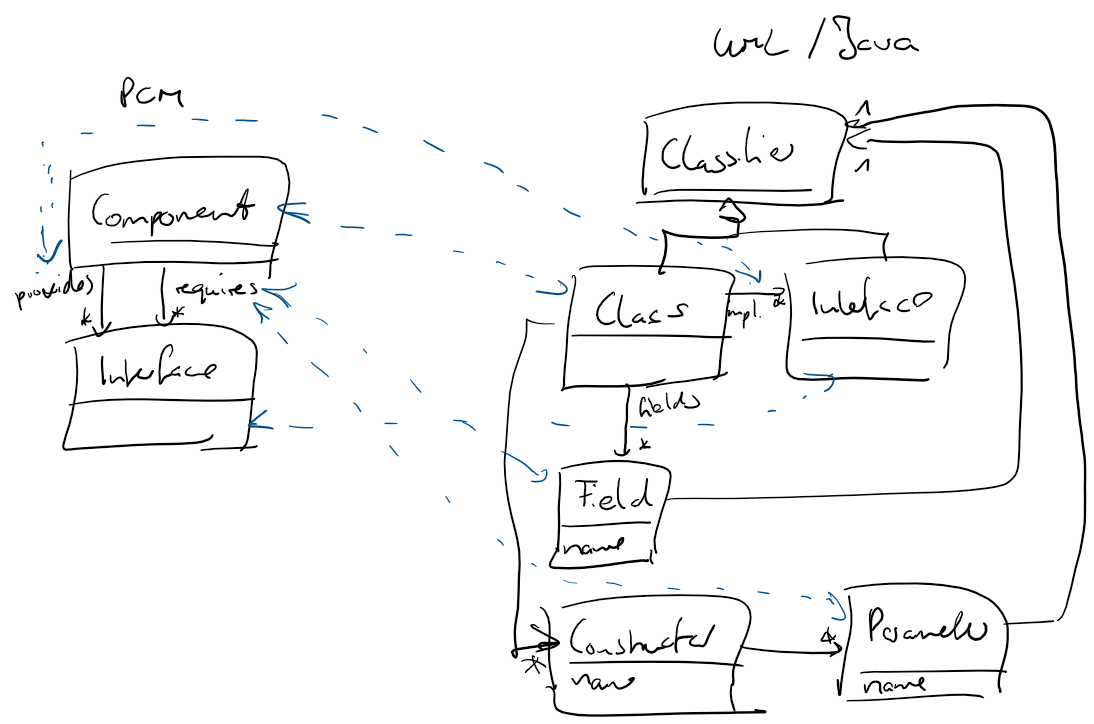
\includegraphics[width=\textwidth]{figures/prologue/introduction/scenario_consistency_relations.png}
    \caption[Consistency relation for PCM and UML/Java]{Extract of consistency relations between component-based architectures in \gls{PCM} and object-oriented design in \gls{UML}/Java according to \cite{langhammer2017a}. Properties are omitted, each element has a least a name.}
    \label{fig:introduction:scenario_consistency_relations}
\end{figure}

\mnote{Consistency relations between \gls{PCM}, \gls{UML} and Java}
Although there are several degrees of freedom to relate \gls{UML} and Java, the extracts that we consider follow a simple one-to-one mapping.
The relevant relations between classes in \gls{PCM} and object-oriented design are depicted in \autoref{fig:introduction:scenario_consistency_relations}.
%We only depict the classes without their properties. Each of them actually has a least a name.
This involves a one-to-one mapping between interfaces and the realization of \gls{PCM} components as classes. 
Provided interfaces in a \gls{PCM} model are realized by interface implementations of the class realizing the component. 
Required interfaces are realized by a field with the type of the interface and constructor parameters that ensure that the required interfaces are set on instantiation of the component.

%% CORRECTNESS
\subsection{Correctness of Transformation Networks}

The central goal of (software) engineering, and thus also the construction of transformation networks as part of the engineering process, is to achieve \emph{correctness} of the developed artifacts.

\subsubsection*{Orchestration Challenge}
\label{chap:introduction:challenges:correctness:orchestration}

% 1. Orchestration problem
\mnote{Single execution of transformations}
When we consider transformations between \gls{PCM} and \gls{UML}, as well as between \gls{UML} and Java, they can transfer each modification to the other models.
For example, adding a \gls{PCM} component creates a class in \gls{UML}, which in turn creates a class in Java.
Although in most cases each transformation only needs to be executed once, there can be situations that require transformation to be executed repeatedly.

\begin{figure}
    \centering
    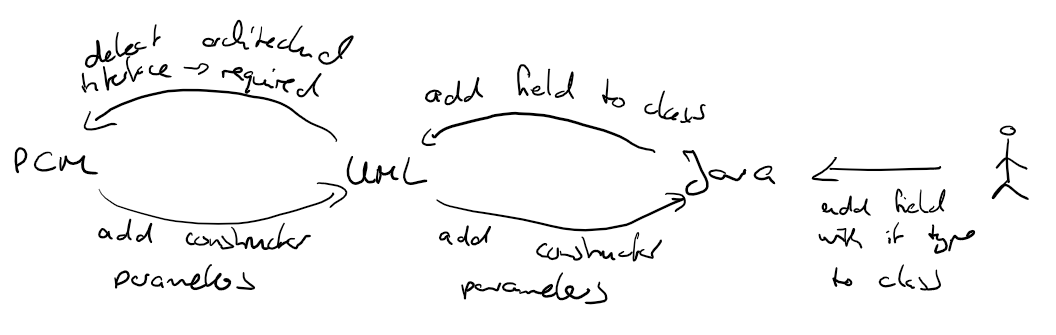
\includegraphics[width=\textwidth]{figures/prologue/introduction/scenario_duplicate_execution.png}
    \caption[Example for transformation orchestration]{Duplicate transformation execution after adding a field representing a required interface to a Java class.}
    \label{fig:introduction:scenario_duplicate_execution}
\end{figure}

\mnote{Multiple executions of same transformation}
In the process depicted in \autoref{fig:introduction:scenario_duplicate_execution}, we assume a system description that contains at least one component and class, respectively, and one interface.
If a developer adds a field to the Java class having the type of the interface, the transformation between \gls{UML} and Java transfers this field to the corresponding \gls{UML} class.
The transformation between \gls{UML} and \gls{PCM} detects that the interface is also represented as an architectural interface in the \gls{PCM} model, thus the field is supposed to represent a required interface in the architectural model.
In consequence, the transformation adds a required interface to the \gls{PCM} component.
Since the consistency relations prescribe each required interface to be represented as a constructor parameter, the transformation also adds a constructor parameter to the class in the \gls{UML} model.
This finally requires the transformation between \gls{UML} and Java to be executed again, because the constructor parameter introduced by the transformation between \gls{PCM} and \gls{UML} must also be added to the Java code.

\mnote{Orchestration challenge}
The example demonstrates that, in general, it is necessary to execute each transformation in a network more than once to achieve a consistent state of the models.
This is always the case if at least two transformations modify the same model, because then the first transformation may need to react the changes of second one again, like in the example the transformation between \gls{UML} and Java needs to react to the one between \gls{PCM} and \gls{UML}, because both modified the \gls{UML} model.
The determination how often and in which order transformations have to be executed is what we call the \emph{orchestration challenge}.

\subsubsection*{Synchronization Challenge}
\label{chap:introduction:challenges:correctness:synchronization}
% 2. Synchronization problem
\mnote{Transformation between \gls{PCM} and Java}
We yet considered that we only have a chain of two transformations, one between \gls{PCM} and \gls{UML} and another between \gls{UML} and Java.
There may, however, also be an overlap of information between \gls{PCM} and Java that cannot be represented in \gls{UML}, which require to also define a transformation between \gls{PCM} and Java.
This is especially the case for behavioral properties, which cannot be expressed in UML class models, such as the functionality defined by Java method implementations and the abstract service specifications in \gls{PCM}.
In consequence, the graph induced by the transformation contains a cycle.

\mnote{Redundancies in transformations}
Instead of only having a transformation for that overlapping information of \gls{PCM} and Java that cannot be expressed across \gls{UML}, the transformation may also contain the relations already expressed across \gls{UML}.
The reasons for that can be independent development and reusability.
Independent development leads to the situation that the developer of the transformation between \gls{PCM} and Java does not know what the transformations to \gls{UML} already express.
Even if the developer has that information, he or she may want to express it again to foster reusability, i.e., to use the transformation between \gls{PCM} and Java in projects in which no \gls{UML} is used or when the transformation is not supposed for a specific network of transformations, comparable to \gls{COTS}.
In consequence, we need to face the situation that multiple transformations propagate the same information, i.e., they contain redundancies.

\begin{figure}
    \centering
    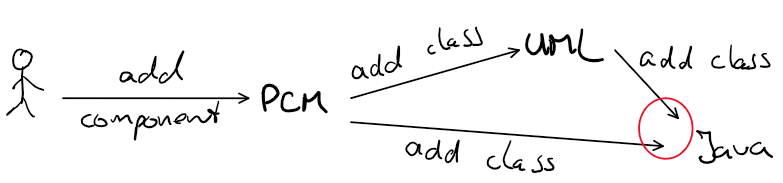
\includegraphics[width=0.8\textwidth]{figures/prologue/introduction/scenario_synchronization.png}
    \caption[Example for transformation synchronization]{Two transformations propagating the same information to Java.}
    \label{fig:introduction:scenario_synchronization}
\end{figure}

\mnote{Two transformation paths creating Java class}
\autoref{fig:introduction:scenario_synchronization} depicts a scenario, in which a user creates a \gls{PCM} component.
The transformations, in consequence, create a \gls{UML} class and, finally, both the transformation between \gls{UML} and Java as well as the one between \gls{PCM} and Java define the creation of an appropriate Java class.
These transformation now have to consider that there may be another transformation that already created that class.
Otherwise, there is the risk of creating a duplicate of that class or of overwriting the already created on.

\mnote{Synchronization challenge}
Such a problem can always occur if two sequences of transformations propagate the same information to the same model. %, like here to Java.
How to achieve that transformations deal with such cases constitutes the \emph{synchronization challenge}.

\subsubsection*{Contradiction Challenge}
% 3. Contradiction problem

\mnote{Equivalence of redundancies}
We have seen that it may be necessary to redundantly define the same consistency relations in different transformations.
This, however, implicitly assumes that they are true redundancies, i.e., that they equally express the relations.
This, in turn, requires all developers to have the same \emph{notion of consistency} between the different tools.

\begin{figure}
    \centering
    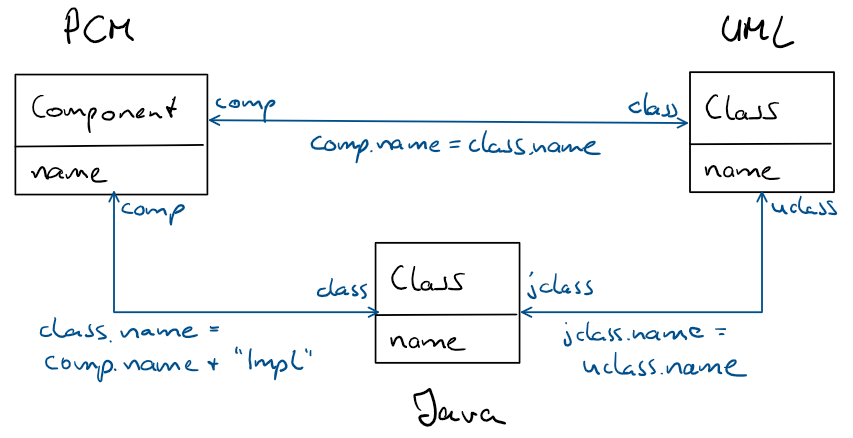
\includegraphics[width=0.8\textwidth]{figures/prologue/introduction/scenario_contradiction.png}
    \caption[Example for transformation contradictions]{Contradicting consistency relations between components in \gls{PCM} and classes in \gls{UML} and Java.}
    \label{fig:introduction:scenario_contradiction}
\end{figure}

\mnote{Contradicting relations}
The example in \autoref{fig:introduction:scenario_contradiction} informally depicts exemplary consistency relations between components and classes.
They are supposed to express that for each a component or class appropriate elements in the other models have to exist with the given name relation.
The constraints for their names can, however, obviously not be fulfilled at the same time.
While the class representations are supposed to have the same name and the \gls{PCM} is also supposed to have the same name as the \gls{UML} class, it is supposed to have the name of the Java class with an \enquote{Impl} suffix, as proposed by \textcite{langhammer2017a}.

\mnote{Different notions of consistency}
Such a situation can occur if the developers of the different transformations have different notions of consistency.
In this case, the performance engineering, who knows about the relation between \gls{PCM} and Java according to the scenario presented in \autoref{fig:introduction:distributed_knowledge}, and the software architect, who knows about the relation between \gls{PCM} and \gls{UML} as well as between \gls{UML} and Java, have different notions about how to represent components in object-oriented design.

\mnote{Non-termination or inconsistent termination}
If the domain experts encode the defined relations in transformations that try to preserve them and execute them after any of the elements is added to a model, the transformations will either terminate in an inconsistent state or never terminate at all.
Executing the transformation for a finite number of times would always result in an inconsistent state, if not removing the element just added by the user.

\mnote{Contradiction challenge}
In consequence, it is important to avoid or detect situations in which transformations with such contradicting constraints in their consistency relations are combined to a network.
We call this the \emph{contradiction challenge}.

\subsubsection*{Problem Statement}

\mnote{Systematic knowledge on correctness challenges}
We have discussed three kinds of issues, which can prohibit that a transformation network terminates consistently, and derived according challenges: orchestration, synchronization and contradiction.
These challenges only exemplify the relevant correctness issues in transformation networks. 
In fact, it is even not systematically known which issues can occur.
Thus, we derive the following general problem statement.

\begin{problemstatement}
    It is unknown how to correctly combine modular and independently developed transformations to networks to yield consistent models after they were changed.
\end{problemstatement}

%% QUALITY PROPERTIES
\subsection{Quality of Transformation Networks}

\mnote{Quality properties of networks}
Like in ordinary (software) engineering, besides the primary goal of producing \emph{correct} artifacts, there are several quality properties that need to be improved.
They can range from properties that are relevant for developers, such as reusability and evolvability, to properties relevant for users, such as performance, scalability and reliability.
This similarly applies to transformation networks as artifacts of the (software) engineering process.

\subsubsection*{Properties and Topology Challenge}

\mnote{Focus on development properties}
In this thesis, we focus on further properties regarding the development of a transformation network, such as reusability and evolvability, rather than properties of its usage, such as scalability.
Reusability is of most importance, because transformation may be used in different contexts within different networks of other transformations.

\begin{figure}
    \centering
    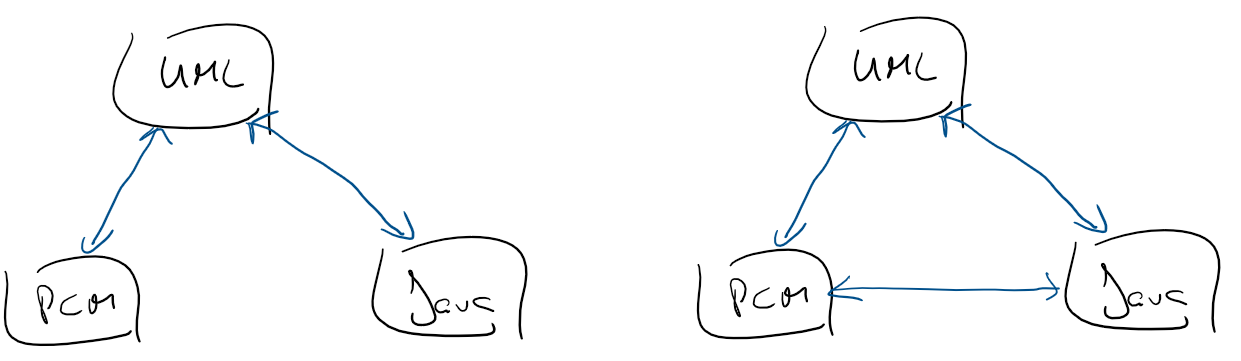
\includegraphics[width=\textwidth]{figures/prologue/introduction/scenario_topologies.png}
    \caption[Example for network topologies]{Different transformation network topologies for \gls{PCM}, \gls{UML} and Java.}
    \label{fig:introduction:scenario_topologies}
\end{figure}

\mnote{Topology extremes}
Consider the two networks depicted in \autoref{fig:introduction:scenario_topologies}.
The networks contain transformation between \gls{PCM} and \gls{UML} as well as between \gls{UML} and Java. 
One of them additionally contains a transformation between \gls{PCM} and Java.
They can be considered as representatives of extremes of transformation networks:
the graph induced by transformations may on the one end be a tree, and on the other be a dense graph.

\mnote{Topologies affect properties}
It is easy to see that properties are directly affected by the network topology.
A dense graph has the benefit of high reusability, because any subset of tools can be used for a development project without loosing consistency.
In the example, the tree network is not applicable in development projects not using \gls{UML}, because then \gls{PCM} and Java cannot be kept consistent.
Additionally, a dense graph profits from universality, because arbitrary relations can be expressed, whereas a tree requires that of three languages there is always one that can express the overlap of the two others.
If there are overlaps between \gls{PCM} and Java that cannot be expressed across \gls{UML}, like discussed for behavioral specifications, a tree cannot be defined.
On the other hand, a tree has the benefit of inherent correctness guarantees.
There are no two paths of transformations between the same two languages.
Thus, no changes can be propagated across two paths to the same model.
This avoid at least two of the three introduced challenges regarding correctness, because neither synchronization problems nor contradictions can occur.

\mnote{Topologies induce trade-offs}
While each kind of topology improves certain properties, it degrades others at the same time.
In other words, topologies induce trade-offs between different properties.
For example, a tree improves correctness, but degrades reusability in comparison to a dense graph.
Deriving how to use this knowledge to mitigate trade-offs and improve different properties at the same time is our \emph{properties and topologies challenge}.

\subsubsection*{Improvement Challenge}

\mnote{Improving properties by specific topologies}
We have seen that topologies directly influence properties of a transformation network.
We will see that with an appropriate strategy of building networks with a specific topology, we can mitigate trade-offs.
Currently, however, there is no known approach and language that supports building transformation networks of specific topologies improving quality properties.
Research approaches did consider approaches and languages for single transformations or for specific composition purposes, such as transformations between the same two languages~\cite{wagelaar2010a,wagelaar2011a}, or chains of transformations~\cite{pilgrim2008a, vanhooff2007UniTI-MODELS}.

\mnote{Improvement challenge}
To relieve the developer from the task of identifying a topology to improve different properties, a universal approach to define an according topology and an appropriate language that supports its definition should be provided.
Investigating such a strategy and design options for an according specification language constitutes our \emph{improvement challenge}.

\begin{integrationcontribution}

\subsubsection*{Integration Challenge}

\mnote{Transformations assume models of specific formalisms}
Finally, we have implicitly assumed that models are developed and thus represented in a format to which transformations can be applied.
Languages for specifying transformations, however, have to assume a well-defined formalism of the languages between they transform~\cite{klare2017models}, thus the models have to follow that formalism.
This is especially problematic for code, which will be relevant for almost every development project.
Although there are tools that wrap code in a specific formalism %, such as JaMoPP~\cite{heidenreich2009a,heidenreich2010a} for using Java code in the Eclipse Modeling Framework, 
recognizing incremental updates of code are still poorly supported.

%\mnote{Models are often implicit}
\mnote{Access to implicit models}
Models are often contained implicitly in code.
This mostly concerns domain models for the software to be developed, but also models to represent code. %of code, such as the Java code representation in the Java Development Tools of the Eclipse Framework~\cite{EclipseJDT}, which has capabilities of recognizing incremental updates.
%\mnote{Lifting artifacts to models}
Lifting such implicit models into a format according to formalisms that allow the application of transformations %and transformation languages 
enables projects using such artifacts to apply transformation techniques to preserve consistency.
For all projects containing such artifacts, this can be seen as a preliminary for applying transformation network, as otherwise only the parts of the projects present in an appropriate formalism can be kept consistent.
In consequence, it can be seen as a \emph{completeness} property of the network.
We denote this as the \emph{integration challenge}.

\end{integrationcontribution}


\subsubsection*{Problem Statement}

\mnote{Impact of topologies and usability for mitigating trade-offs unknown}
We have discussed that topologies affect different correctness and quality properties of transformation network and that they impose trade-offs between them.
It is unclear how that insight can be used to systematically improve different properties by building transformation networks of specific topologies.
Thus, we derive the following problem statement.

\begin{problemstatement}
    It is unknown how to systematically mitigate trade-off decisions between correctness and quality properties, such as reusability and comprehensibility, of transformation networks.
\end{problemstatement}


\subsection{Challenges Overview}

\begin{figure}
    \centering
    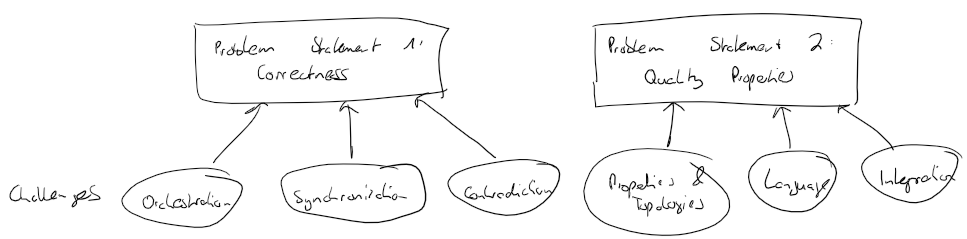
\includegraphics[width=0.9\textwidth]{figures/prologue/introduction/challenges.png}
    \caption[Problem statements and challenges]{The two identified problem statements and their challenges.}
    \label{fig:introduction:challenges}
\end{figure}

\mnote{Summary of problems statements and challenges}
We have discussed several issues regarding the construction of transformation networks.
We summarize the problem statements and challenges in \autoref{fig:introduction:challenges}.
We made two central problem statements, one regarding the correctness of networks and another regarding the improvement of quality properties.
Each of these problems is driven by three challenges.
We identified orchestration, synchronization and contradiction to be central challenges for constructing \emph{correct} transformation networks.
For the improvement of quality properties, we emphasized that the relation between properties and topologies challenges the identification of a topology to mitigate property trade-offs and to define an appropriate strategy and language for that.
\begin{integrationcontribution}
To achieve completeness of a network, we identified the integration challenge. % to integrate all kinds of artifacts into a transformation-based consistency process.
\end{integrationcontribution}


%%
%% RESEARCH OBJECTIVE
%%
\section{Research Objective}

\mnote{Research questions, assumptions and contributions}
We have identified specific challenges that we have to deal with when constructing transformation networks and generalized them into two central problem statements.
In the following, we derive our research goal and the actual research questions that we will answer in this thesis in response to the defined problem statements.
Afterwards, we summarize the context and the assumptions that we make in our work.
Finally, we give an overview of the contributions that we make to answer the defined research questions.

\subsection{Research Goal and Questions}

The central goal of our research can be summarized as follows.
\begin{researchgoal}
Define a notion of correctness for networks of modular, independently developed transformations and classify relevant quality properties.
Provide approaches to systematically improve correctness and quality properties of transformation networks either by construction or by analysis.
\end{researchgoal}

\mnote{Benefits of achieving goal}
The benefits of achieving that goal are twofold.
First, researchers and transformation developers both gain systematic knowledge about how to achieve correctness and improve quality properties in transformation networks.
Second, transformation developers are provided with concrete techniques and languages that help to achieve correctness and improve other properties either by construction or at least by analysis.

\mnote{Parts of research goal}
The research goal consists of two parts, one regarding correctness of transformation networks and one regarding improvement of its quality attributes.
For each of these parts we identify appropriate and fine-grained research questions.

% \subsection*{Properties of Transformation Networks}

% Overall Goal: We want to find out which properties are relevant when building transformation networks and how they are affected by different topologies. This is supposed to help finding ways of systematically improving those properties.

% \begin{researchquestions}{1}
% 	\item \researchquestion{rq:properties}{What are relevant properties and topologies of transformation networks and how do they depend?}
% 	\begin{subresearchquestions}
% 		\item \researchquestion{rq:properties:properties}{Which functional and non-functional properties are relevant when defining transformation networks?}
% 		\item \researchquestion{rq:properties:topologies}{How can network topologies be classified regarding the properties identified in \researchquestionref{rq:properties:properties}?}
% 	\end{subresearchquestions}
% \end{researchquestions}

% \begin{enumerate}[label=\itshape RQ \arabic*.]
% 	% Issue classification
% 	\item Which issues can occur when independently developed \acp{BX} are combined to a network?
% 	\begin{nestedenum}
% 		\item Which failures can occur, when \acp{BX} are combined to a network?
% 		\item What mistakes can be made that lead to failures?
% 		\item How can these mistakes be categorized regarding conceptual levels in the specification process for \acp{BX}?
% 	\end{nestedenum}
% 	\item How are properties of transformation networks affected by the topology?
% 	\begin{nestedenum}
% 		\item Which properties are relevant when defining networks of \acp{BX}?
% 		\item Which topologies of network exist and how do they affect that properties?
% 	\end{nestedenum}
% \end{enumerate}

% \subsubsection*{Evaluation}

% Keine dezidierte Evaluation, lediglich Argumentation


\subsubsection*{Building Correct Transformation Networks} % Correctness of Transformation Networks?

\mnote{Correctness questions}
The first part of our research goal concerns correctness of transformation networks.
We want to know what \emph{correctness} means for transformation networks and which aspects of correctness we can achieve for every network, in particular, which of them we can achieve by proper construction of the single transformations, which we can analyze and for which we need to deal with potential incorrectness until their execution.

\begin{researchquestions}
	\researchquestion{rq:correctness}{When should networks of independently developed transformations be considered \emph{correct} and how can correctness be achieved?}
	\begin{subresearchquestions}
		\subresearchquestion{rq:correctness:notions}{What are relevant notions of correctness in transformation networks and how can they be formalized?}% EV: Argumentation
		\subresearchquestion{rq:correctness:compatibility}{When are the constraints induced by transformations contradictory and how can that be analyzed?}% EV: Proof and empirical application in case study
		\subresearchquestion{rq:correctness:synchronization}{Which requirements must a transformation fulfill for being used in a network in comparison to using it on its own?}% EV: Proof and empirical application in case study
		\subresearchquestion{rq:correctness:orchestration}{How can transformations in a network be orchestrated and which properties can such an orchestration strategy fulfill?}% EV: Argumentation, Examples
		\subresearchquestion{rq:correctness:errors}{Which errors can occur in transformation networks, how can they be classified regarding their avoidability and how severe are they?}% EV: Case Study
	\end{subresearchquestions}
\end{researchquestions}

\mnote{Relation between question and challenges}
\autoref{rq:correctness:notions} is the fundamental question to precisely define what \emph{correctness} means, beyond our yet informally given notion.
\autoref{rq:correctness:compatibility}, \autoref{rq:correctness:synchronization} and \autoref{rq:correctness:orchestration} directly map to the previously identified challenges regarding orchestration, synchronization and contradiction.
Finally, \autoref{rq:correctness:errors} asks for the inverse, i.e., for the case when errors occur due to incorrectness, to find out how incorrectness manifests and how severe it is.


% \begin{enumerate}[label=\itshape RQ \arabic*.]
% 	\setcounter{enumi}{2}
	% % Contradiction analysis
	% \item How can transformations be analyzed regarding contradictions in specified constraints?
	% \begin{nestedenum}
	% 	\item What is an appropriate formalism for describing transformations that can be analyzed regarding potential contradictions?
	% 	\item Which kinds of contradictions can be detected by analyzing transformations following a specific formalism?
	% \end{nestedenum}
	% % Issue avoidance by construction
	% \item How can interoperability of independently developed \acp{BX} be achieved by construction?
	% \begin{nestedenum}
	% 	\item Which kinds of mistakes can be avoided by construction of the individual \acp{BX}?
	% 	\item How can we prove that those mistakes and only those mistakes can be avoided by construction?
	% 	\item How can each of these mistakes be avoided by a transformation developer during independent development of a single \acp{BX}?
	% \end{nestedenum}
	% % Orchestration
	% \item What is an appropriate strategy for orchestrating independently developed \acp{BX} to perform a fixed-point iteration?
	% \begin{nestedenum}
	% 	\item Which strategies for orchestrating a network of \acp{BX} exists and what are their properties?
	% 	\item How should those properties be weighted and which of the strategies should be chosen for orchestration?
	% \end{nestedenum}
% \end{enumerate}

% \subsubsection*{Evaluation}

% \gqm{Functionality}{The analysis can be used to find contradictions in specifications}
% {Does the analysis find contradictions if they exist?}
% {Recall: Ratio of true positives to true positives + false negatives}
% \qm{Does the analysis find contradictions although they do not exist?}
% {Precision: Ratio of true positives to true+false positives}
% \qm{Does the analysis find non-contradictions although they exist?}
% {Ratio of false negatives to false+true negatives}

% \gqm{Functionality}{The techniques to avoid mistakes by construction actually avoid interoperabililty issues}
% {Are the identified failures that can occur complete?}
% {Ratio of number of identified failures to total number of failures}
% \qm{Are the relations of identified mistakes to identified failures correct?}
% {Ratio of failures resolved by fixing the identified mistake to all failures}
% \qm{Does the application of avoidance techniques lead to interoperable transformations?}
% {Ratio of changes that are propagated correctly to those that are not propagated correctly}

% \gqm{Applicability}{The techniques can be applied independently to single transformations}
% {Are there cases in which information about other transformations are necessary to solve issues?}
% {Ratio of number of fixes that require information about other transformation to total number of fixes with user interactions\\
% Ratio of number of fixes that require information about other transformation to total number of fixes without user interactions}


\subsubsection*{Improving Quality Properties of Transformation Networks}

\mnote{Quality properties questions}
The second part of our research goal concerns quality properties of transformation networks.
We want to known how we can systematically improve the quality of transformation networks. 
This includes the identification of properties that are relevant when building transformation networks and how they are affected by different topologies. 
We use this to systematically derive a proper construction approach achieving a specific topology that resolves trade-offs between quality properties. 
%Second, by including models that were not explicitly modelled as such before to allow their integration into a transformation-based consistency process.

\begin{researchquestions}
	\researchquestion{rq:quality}{How can quality properties of transformation networks be improved systematically?}
    \begin{subresearchquestions}
        \subresearchquestion{rq:quality:properties}{What are relevant properties and topologies of transformation networks?} % EV: Argumentation
		\subresearchquestion{rq:quality:topology}{How can topologies of transformation networks improve quality properties of transformation networks?} % EV: Argumentation
		\subresearchquestion{rq:quality:language}{How can a specialized language support the specification of a network topology that improves quality properties?} % EV: Proof-of-concept and case study
        \begin{integrationcontribution}
            \subresearchquestion{rq:quality:process}{How can software development artifacts be integrated into a transformation-based consistency process?} % EV: Case study
        \end{integrationcontribution}
	\end{subresearchquestions}
\end{researchquestions}

\mnote{Relation between question and challenges}
\autoref{rq:quality:properties} and \autoref{rq:quality:topology} directly map to the properties and topologies challenge for identifying how topologies affect properties and how to use them for improving quality properties.
\autoref{rq:quality:language} then maps to the language challenge for designing an appropriate language that supports the construction of an appropriate topology.
\begin{integrationcontribution}
    Finally, \autoref{rq:quality:process} maps to the integration challenge for lifting artifacts to models that can be used in a transformation-based consistency process.
\end{integrationcontribution}

% \begin{enumerate}[label=\itshape RQ \arabic*.]
% 	\setcounter{enumi}{5}
% 	\item How can a topology of transformation be build that optimizes non-functional properties of transformation networks?
% 	\begin{nestedenum}
% 	    \item How can transformation contradictions be avoided by language design? %uniqueness of consistency specification and consistency among themselves achieved by language design?
% 	    \item How can modularity be achieved in a way such that an arbitrary set of metamodels for which consistency is specified can be used in an actual project?
% 	\end{nestedenum}
% 	% Building tree topologies
% 	\item How should a language specific for multi-model consistency be defined that supports a non-functional property-optimizing topology definition?
% 	\begin{nestedenum}
% 		\item What are the design decisions for such a language?
% 	\end{nestedenum}
% \end{enumerate}

% \subsubsection*{Evaluation}

% \gqm{Functionality}{Concept and language can achieve consistency between several models}{How many model changes in a case study can be properly kept consistent?}{Ratio of successfull test cases}

% \gqm{Practicality}{The assumption of defining a tree of \commonalities is achievable in practice}{Is the definition of cross-tree relations necessary in a case study?}{Number of cross-tree relations in a case study compared to number of relations}

% \gqm{Practicality/Benefit}{A specific language improves conciseness of consistency specifications}{How much more concise is the specification for a case study compared to a definition with direct transformations?}{Number of SLOC with \commonalities compared to number of SLOC with \reactions for same case study}

% Diskussion: Erreichen der Modularität auch evaluieren? Ist per Konstruktion gegeben, könnte man aber natürlich auch noch auswerten (bringt aber nichts).



%% CONTEXT AND ASSUMPTION
\subsection{Context and Assumptions}
\label{chap:introduction:objective:assumptions}

\mnote{Model-driven processes}
In this thesis, we consider the context of model-driven development processes, be it software or software-intensive technical systems.
Thus, we assume that the system under construction is described by several models containing information about different extracts or properties of the systems.
We assume that they usually share some overlap of information.
Our discussions will focus on software development artifacts.
As long as they follow the same formalisms, however, the insights and techniques may be applied to artifacts from arbitrary domain.

\mnote{Distributed knowledge and independent development}
We assume that the knowledge about different transformations to be combined to a network is distributed.
To foster the development of transformations that can be used as \gls{COTS}, we assume that transformations are developed independently.
Thus, transformations may not be adapted to be used within transformation networks.

\mnote{Consistency relation types}
We do not restrict the kinds of relations between models to keep consistent  in any way.
We will, however, discuss different types of consistency and their relations to different kinds of processes to preserve consistency in \autoref{chap:networks:notions:types}.
In fact, our contributions, although theoretically not restricted to that, will be best applicable to a kind of \emph{structural} dependencies rather than \emph{behavioral} dependencies.

\mnote{Semi-automatism}
Finally, transformations may not always be able to restore consistency on their own, because necessary information to do so is missing.
For example, a developer may introduce a class in Java and a transformation has to decide whether that class shall represent a component in \gls{PCM} or not.
That problem can either be solved by requiring the class to fulfill certain patterns, like containing \enquote{Component} in the class name, or by asking the user about his intent.
In cases where information is transformed to a semantically richer model, often further information about how to transform is necessary.
\textcite[p. 57]{kramer2017a} provides a classification for different levels of automation, starting from no automation over suggestions and semi-automated repair to fully automated repair.
In this thesis, we assume that consistency is preserved in a fully automated way, thus excluding the semi-automatic case.
We will finally discuss how our finding generalize to the case where user decisions need to be included.

% Focus on development, rather than usage -> motivate comprehensibility with developer, not with user


%% CONTRIBUTIONS
\subsection{Contributions}

\begin{figure}
    \centering
    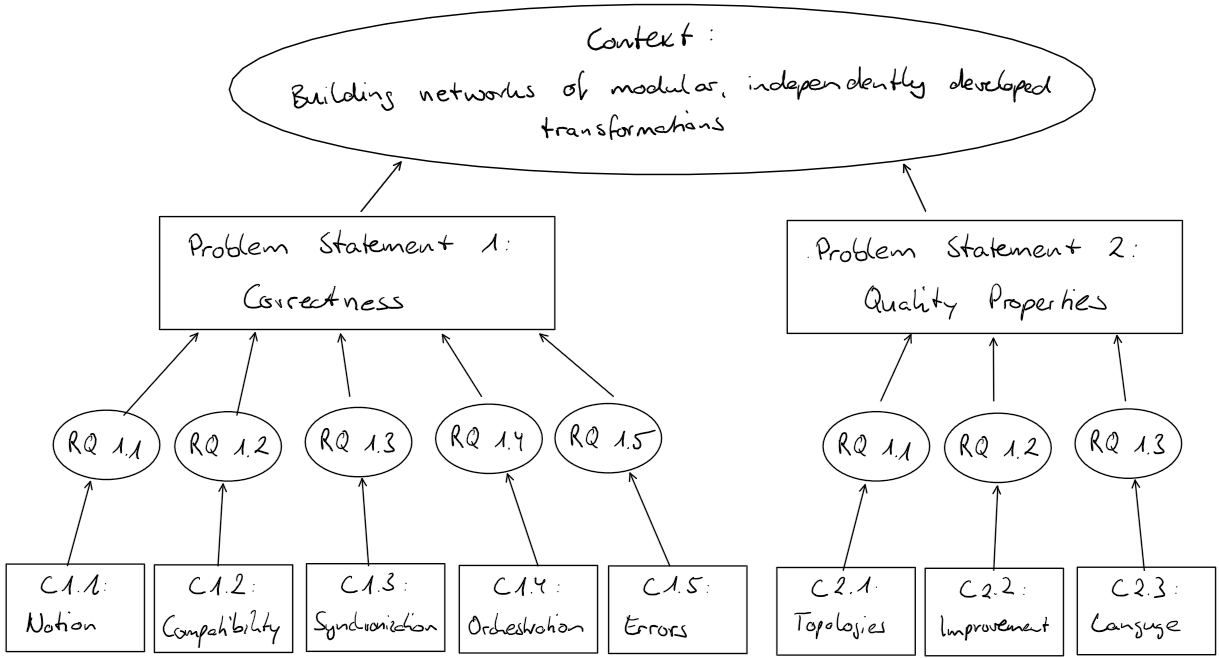
\includegraphics[width=\textwidth]{figures/prologue/introduction/context_problem_eq_contribution_relations.png}
    \caption[Context, problems, research questions and contributions]{Relation between context, problem statements, research questions and contributions}
    \label{fig:introduction:context_problem_rq_contribution_relations}
\end{figure}

\mnote{Contribution structure}
The contributions that we make in this thesis are structured along the same dimensions as the problems and the research questions, namely correctness and quality properties.
The contributions directly map to the research questions.
\autoref{fig:introduction:context_problem_rq_contribution_relations} gives an overview of the relations between the context of our work, the problem statements, the research questions and the contributions that we make.

We make the following contributions regarding transformation network correctness.
\begin{contributions}
    \contribution{contrib:correctness:notion}{Notion}{We discuss different notions of correctness for transformation networks and precisely define the one relevant for our context. We derive that compatibility, synchronization and orchestration constitute the relevant correctness notions.}
    \contribution{contrib:correctness:compatibility}{Compatibility}{We precisely define a notion of compatibility to express when transformations contain contradictory constraints. We propose an approach that validates compatibility of transformations and prove its correctness.}
    \contribution{contrib:correctness:synchronization}{Synchronization}{We discuss how synchronization can be achieved for transformations defined with existing transformation languages. We prove that transformations fulfilling a specific property can be applied in transformation networks. %We make a case distinction over all possible synchronization cases to derive a complete list of problematic synchronization cases. 
    We provide an algorithm to execute the transformation in that case and propose a strategy to fulfill the required property by construction.}
    \contribution{contrib:correctness:orchestration}{Orchestration}{We prove that transformations, in general, can neither be executed only once nor an arbitrary number of times in a fixed-point iteration without the risk of non-termination. We prove that finding an execution order of the transformations that yields consistent models is an undecidable problem and discuss why we cannot make restrictions to the transformations to achieve its decidability. We propose an algorithm for orchestration that executes the transformations according to a well-defined strategy and helps to find the cause in cases it does not return consistent models.}
    \contribution{contrib:correctness:errors}{Errors}{We systematically derive which errors can occur when correctness of a transformation network is not given. We also empirically evaluate the probability of the different errors to occur to classify their severity and thus the importance of avoiding them.}
\end{contributions}

We make the following contributions regarding the improvement of quality properties of transformation networks.
\begin{contributions}
    \contribution{contrib:quality:topologies}{Topologies}{We discuss how different quality properties of transformation networks are affected by the network topology. We derive that trade-off decisions have to be made between the improvement of different properties.}
    \contribution{contrib:quality:improvement}{Improvement}{We propose a strategy for building a specific network topology based on auxiliary models, which make the consistency relations explicit in terms of models rather than transformations. We show that this approach systematically improves different quality properties and mitigates necessary trade-off decisions.}
    \contribution{contrib:quality:language}{Language}{We propose a specialized language for the definition of a network according to the strategy of \autoref{contrib:quality:improvement}. 
    We discuss different design options for the language and its operationalization.}
    \begin{integrationcontribution}
        \contribution{contrib:quality:integration}{Integration}{We propose an approach for lifting existing models, which are only implicitly encoded in code, to an explicit representation according to a modeling formalism. It enables the usage of implicit models in a model-driven development process.}
    \end{integrationcontribution}
\end{contributions}


\subsection{Expected Benefits}

\mnote{Overall benefits}
The contributions that we make in this thesis provide several benefits for researchers, developers of transformations and transformation networks, as well as transformation (network) users.
All of them profit from systematic knowledge about what \emph{correctness} means for transformation networks, how correctness is affected and can be guaranteed, and about relevant \emph{quality properties} in transformation networks as well as how they can be improved.
The contributions, however, have an intended focus on supporting transformation and transformation network developers. 

\mnote{Benefits for researchers}
Researchers can base on our definitions for correctness of transformation networks and can thus precisely contribute to particular parts of the defined correctness notions, e.g., by approaches to achieve correctness, with explicitly knowing how and which kinds of potential errors of transformation networks are affected by that.
Additionally, they can base further research on the insights about trade-offs between quality properties induced by different network topologies.

\mnote{Benefits for transformation (network) developers}
The developers of actual transformation networks can be separated into the developers of the individual transformations and the ones combining them to a network.
The development of individual transformations is supported by the provision of systematic approaches to build transformations that can be used within networks, especially in terms of supporting synchronization.
Transformation network developers benefit from the knowledge that they have to deal with undecidability of orchestration, i.e., of finding an execution order for transformations.
They also benefit from approaches to validate transformations they want to combine regarding compatibility, an actual and practical orchestration strategy to execute transformations, and an approach to build networks that mitigate trade-offs between quality properties.

\mnote{Benefits for transformation (network) users}
Finally, the users of a transformation network, i.e., the ones who develop a system using a transformation network to preserve consistency of its artifacts, benefit from the ability to use networks, for which correctness was systematically achieved, at all.
They also profit from an orchestration strategy that supports them in finding and understanding the reasons why the networks may not be able to process certain changes to preserve consistency.



%%
%% OUTLINE
%%
\section{Thesis Outline}

\todo{Write outline}

First some general considerations, notation, formal basis etc.

Structured along correctness / quality properties.
Each chapter maps to one of the defined contributions

Reading process: Correctness and quality properties are almost independent, so possible to start with any of the parts. Within the parts, consecutive reading recommended.
However:
Correctness: Start with notion and compatibility chapter, then proceed with any of the following, no strict dependencies. Errors hard to understand without rest.
Quality (read first chapter of correctness first): First three chapters depend on each, so do not jump. 
\begin{integrationcontribution}
    Fourth chapter (integration) is independent.
\end{integrationcontribution}

In each chapter, we recapture the research question we want to answer in the beginning and point out the contribution that we make with that chapter and we close the chapter with the central insights that the chapter gave.


%%
%% OLD: COPIED FROM PAPERS
%%

%\begin{copiedFrom}{DocSym}

%\section{From DocSym}
%\todo{Clearly introduce running example, removed from content section!}
%\todo{Introduce set notation, say that is it not practically applicable and a strong simplification, but just used to illustrate the problems and solution approaches} % Done at the end
%\todo{Introduce transitive operator R1 o R2 = (R1 u R2) * $\backslash$ (R1 u R2)} % Done at the end

%\todoConference{The problem the research intends to solve, the target audience of this research, and a motivation of why the problem is important and needs to be solved.}

%\acl{MDSD} proposes the usage of models as primary artifacts of the %software 
%development process~\cite{stahl2006a}. 
%Those models describe different system properties for the interests of specific stakeholders, known as \emph{multi-view modelling}, or at different abstraction levels, representing refinements. In both cases, the models describe the same system and are thus not disjoint but contain redundant or dependent information. 
%\todoErik{Wieder: Die beschreiben ja keine Abstraktion, die sind eine Abstraktion. \enquote{Domains of the system} klingt auch komisch, ich weiß zwar, was Du meinst, aber nenne es nicht \enquote{domain}, sondern lieber \enquote{properties}}
%Developers must be aware of those dependencies to ensure that models are modified consistently. 
%Otherwise, the deployed software, which is derived from those models, will potentially not operate correctly.
%\todoErik{Lenkt den Fokus etwas zu stark auf Korrektheit, die wir nicht formal beweisen. Es geht ja nicht nur darum, daß die Software nicht korrekt arbeitet -- möglicherweise tut sie das ja, obwohl die Modelle inkonsistent sind, und das Problem tritt erst bei der Wartung/Evolution auf.}

%In large software systems, a single developer cannot know about all dependencies~\cite{petrenko2008a}, %which can be formulated as \emph{consistency constraints} and 
%in the following referred to as \emph{consistency relations}, which inevitably leads to inconsistencies. 
%Therefore, automated mechanisms that preserve consistency according to those consistency relations are necessary. 
%For that purpose, incremental, bidirectional model transformations %or specialized model synchronization approaches 
%are commonly used. However, most research considers \emph{binary transformations}, restricted to pairs of models, and does not explicitly consider consistency between more than two models~\cite{stevens2017a}, which we refer to as \emph{multi-model consistency}.
%In general, keeping more than two models consistent is currently not researched well.
%Model transformations can either be specified imperatively or declaratively. They differ in who operationalizes the preservation of constraints that have to hold, in the first case the transformation developer and in the second case an automated mechanism of the transformation language. This is why we do not explicitly distinguish these approaches, as all problems apply to both approaches and only different roles have to deal with them. 
% Model transformations can either be specified imperatively, such that the transformation developer has to define how to react to a change, or declaratively, such that the transformation developers only the constraints that have to hold and an automated mechanism derives an imperative operationalization from that.
% We will not explicitly distinguish these approaches, as the identified problems and our solution proposals apply to both. The only difference is that in imperative approaches the transformation developer has to deal with them and in declarative approaches the developer of the transformation language has to consider them when defining the generation of the operationalization.

% Although it is possible to combine binary transformations by transitively executing them, it is yet unclear what problems may arise from that, especially if each transformation is developed independently and treated as a black box.
% We will exemplify this on the simple example in \autoref{fig:prologue:binary_combination_example}, in which consistency relations define a mapping of a component in an \ac{ADL} to a class in object-oriented design, which is again represented by an implemented class in Java code. 
% The name of the class is defined to be the component name with an \enquote{Impl} suffix (cf.~\cite{langhammer2017a}).
% When all these relations are expressed in transformations, it is, for example, possible that both transformations from \ac{ADL} to Java, once over \ac{UML} (\ref{fig:prologue:binary_combination_example:R1} and \ref{fig:prologue:binary_combination_example:R2}) and once directly (\ref{fig:prologue:binary_combination_example:R3}), create a Java class after creating an \ac{ADL} component.
% We refer to that as an \emph{interoperability problem}.
% The transformation specification %or its execution engine 
% would have to avoid an overwrite and therefore have to consider dependencies between transformations, using, for example, a shared trace model.
% In general, an interoperability problem is an unexpected behavior of transformations, which only occurs if they are executed transitively, but not if each is executed on its own. %, although all preserve the same consistency relations.

% Additionally, it is easy to see that %specifying multi-model consistency with combinations of 
% combining binary transformations leads to trade-off decisions.
% The ternary relation %between the three metamodels 
% can either be expressed by three binary transformations between all pairs of metamodels or by two binary transformations with the third being %expressed by the transitive 
% the combination of the two others.
% The first option leads to redundancies in the specifications, as each pair of transformations has to have an equal semantics than the third.
% For example, the \ac{ADL} to Java transformation for \ref{fig:prologue:binary_combination_example:R3} must be equal to the combination of the transformations \ac{ADL} to \ac{UML}~(\ref{fig:prologue:binary_combination_example:R1}) and \ac{UML} to Java~(\ref{fig:prologue:binary_combination_example:R2}).
% Consequently, those transformations may be incompatible if not correctly defined, e.g., by leaving out the suffix addition in the transformation for \ref{fig:prologue:binary_combination_example:R3}.
% %As an alternative, the second option is express the ternary relation with two binary consistency relation specifications.
% %For example, specification \ref{fig:example:R3} can be interpreted as a combination of \ref{fig:example:R1} and \ref{fig:example:R2}.
% An alternative is to omit the transformation for \ref{fig:prologue:binary_combination_example:R3} by transitively executing the two others.
% However, in this case, modularity is reduced, because it is not possible to use only Java and the \ac{ADL} to develop a specific system and omit the \ac{UML}.
% %Additionally, comprehensibility decreases, because the relation between \ac{ADL} and Java is only expressed transitively. 
% %This becomes more problematic if transformation paths have a length higher than two.
% We refer to this as \emph{specification trade-offs}.

% \begin{figure}
%     \centering
%     \begin{tikzpicture}

    \node[uml class, align=center, minimum width=10em] (component) {\umlcomponentlabel\\[-0.3em] \small PaymentSystem};
    \node[above=0em of component.north, anchor=south] (adl_label) {\textit{ADL}};
    
    \node[uml class, minimum width=10em, below left=2.15em and 7.5em of component.south, anchor=north, font=\small] (uml_class) {PaymentSystemImpl};
    \node[above right=0em and 1em of uml_class.north west, anchor=south west] (uml_label) {\textit{UML}};
    
    \node[draw, minimum width=10em, below right=2.15em and 7.5em of component.south, align=left, anchor=north, font=\small] (java_class) {
    \textbf{class} PaymentSystemImpl \{ \\[-0.3em]
        \hspace{1em} {\tiny // \ldots} \\[-0.3em]
    \}
    };
    \node[above left=0em and 1em of java_class.north east, anchor=south east] (java_label) {\textit{Java}};
    
    \draw[latex-latex, dashed, thick=false] (component) -- node[above left=-0.5em and 0.5em] {\mylabel{fig:prologue:binary_combination_example:R1}{$R_1$}} (uml_class);
    \draw[latex-latex, dashed, thick=false] ([yshift=-1.5em]uml_class.north east) -- node[above] {\mylabel{fig:prologue:binary_combination_example:R2}{$R_2$}} ([yshift=-1.5em]java_class.north west);
    \draw[latex-latex, dashed, thick=false] (component) -- node[above right=-0.5em and 0.5em] {\mylabel{fig:prologue:binary_combination_example:R3}{$R_3$}} (java_class);
    
\end{tikzpicture}
%     \caption{Example models with binary consistency relations}
%     \label{fig:prologue:binary_combination_example}
% \end{figure}

%Although specific approaches for expressing multiary relations, rather than using combinations of binary relations, could be developed, there are some reasons for adhering to binary transformations.
%Instead of developing approaches to express multiary consistency relations, there are reasons to adhere to binary transformations, and to research their combinability.
%As stated by \textcite{stevens2017a}, %there are especially strong practical reasons, as 
%it is hard enough to think about binary relations. %between pairs of models.
%Defining multiary relations would require a knowledge about the relations between all metamodels used to describe a system.
%Additionally, each domain expert, who specifies transformations, %in practice, 
%will usually only have knowledge about the relations between two or at most a rather limited set of metamodels. %, but not of all involved metamodels. %, which would be necessary to define multiary relations.
%Thus, it is a natural goal to make the modular specification of consistency based on binary transformations possible.
%In the proposed thesis, 
%We therefore plan to make the following contributions to research on multi-model consistency preservation:
%\todoErik{Ich fänd's cool, wenn die Probleme auch irgendwie hervorgehoben sind, und Du die Beiträge schon auf die Probleme beziehen kannst, also Mini-PIBA für jedes Deiner identifizierten Probleme. Würde aber erst die Probleme formulieren, dann den IBA-Teil so wie unten (wobei bei manchen noch die Beschreibung des Benefits fehlt).}
% \begin{description}[leftmargin=\parindent]
%     \item[Transformation interoperability.] %Under the assumption that 
%         When several binary transformations are developed independently, they must be combinable in a black box manner, introduced as the \emph{interoperability problem}. We will therefore identify problems that can arise from that combination %of transformations 
%         and develop a catalog of patters that can be followed by the transformation developer or language to achieve \emph{non-intrusive} interoperability of binary transformations.
%     \item[Decomposition of consistency relations.] 
%         The usage of binary transformations for multi-model consistency preservation leads to \emph{specification trade-offs} regarding essential challenges. We will provide a classification of those challenges and investigate the influence of the way in which transformations are specified on them.
%         %Decomposing the underlying consistency relations into independent sub-relations allows a partial optimization regarding those challenges.
%         %We will therefore investigate how consistency relations can be decomposed into independent subsets.
%         We will especially investigate how consistency relations can be decomposed into independent subsets, as this allows a partial optimization regarding those challenges.
%     %We will identify relevant properties of consistency specifications, which have to be considered when defining those specifications as they introduce trade-off decision. We already motivated some of those properties above and give a more detailed overview in \autoref{sec:multimodelconsistency}.
%     \item[Make common concepts explicit.] 
%         Metamodels often represent the same concepts in different ways. As another contribution to reduce \emph{specification trade-offs}, we propose an approach to make these common concepts explicit to improve comprehensibility of transformations and to improve their modular reuse.
% \end{description}

% We propose an approach for multi-model consistency based on \aclp{VOMM}. 
% In those virtual metamodels, dependencies between metamodels, which we refer to as \emph{consistency relations}, are made explicit by representing common concepts, whereas in model transformations, which we refer to as \emph{consistency preservation specifications}, they are specified implicitly. 
% The envisioned benefit is an inversion of the above mentioned properties. 

%Throughout this paper, we use a simplified notation for metamodels and heir consistency relations to ease their illustration. 
%We consider metamodels to be sets of elements and consistency relations to be sets of symmetric, binary relations between those elements.
%To ease the representation of combinations of consistency relations, we define the concatenation operation for two consistency relations $R_1$ and $R_2$ as:
%\begin{equation*}
%    R_1 \concat R_2 \coloneqq \{(x,y)\, |\, \exists t: x\, R_1\, t\, R_2\, y \}.
%\end{equation*}
%This is the subset of the transitive closure of two relations that contains only the relations transitively defined over $R_1$ and $R_2$.
%It can be also expressed as the natural join of $R_1$ and $R_2$ with an additional projection that removes the common elements of both relations.
%The operator is commutative since the relations are assumed symmetric.

% \todoErik{Würd ich bei so einem kurzen Paper weglassen. (Ich würde es auch oft bei langen Papern weglassen. :-))}
% In this paper, we first discuss related work in \autoref{sec:relatedwork}. 
% In \autoref{sec:approach}, we give an overview of our planned contributions by explaining the problems in detail and sketching our solution approaches. %we first discuss interoperability problems arising from the combination of independently developed binary transformations and give an overview on envisioned solution patterns.
% %We then give an introduction to the yet identified challenges inducing trade-off decisions during transformation development.
% %From this, we derive the consideration of consistency relation composition and an approach to make common concepts explicit.
% % We then discuss problems arising from the black-box combination of binary transformations and give an overview on envisioned solution patterns.
% % In \autoref{sec:vomms}, we introduce our approach to make overlaps of metamodels explicit to improve properties of multiary consistency specifications.
% Finally, we discuss the current state and planned evaluation in \autoref{sec:status} and conclude the paper in \autoref{sec:conclusion}.


% \begin{itemize}
%     \item Motivation MDSD
%     \item Several models describe single system
%     \item Information overlap between models, e.g. component architecture and code, ref to Michael
%     \item Developers must be aware of redundancies and dependencies, otherwise inconsistencies
%     \item Best: Make redundancies/dependencies explicit for (semi-)automated mechanisms for preserving consistency
%     \item Incremental model transformations can be used (refs) or specialized model consistency or model synchronization approaches (refs)
%     \item Existing approaches only concern consistency preservation between instances of two metamodels
%     \item If more than two models are involved, these approach would require that consistency preservation is executed transitively
%     \item From that, problems arise
%     \begin{itemize}
%         \item Inconsistent consistency specifications: Consistency specifications between different metamodels must be consistent. E.g. having 3 metamodels, a consistency specification between two of them can be contradictory to the two other
%         \item Consequence: Result of a modification depends on the order in which consistency specification are evaluated or even results in propagation cycle due to alternating changes -- EXAMPLE
%         \item Ordering problem: Preserving consistency after a change can require several changes in other models. The order in which they are executed can produce different results -- EXAMPLE
%         \item Confluence problem: Changes can be propagated across several paths, if more than two models are involved. This can result in conflicts, if the propagation confluences in one model. E.g. it can be necessary to create a metaclass instance in that model to preserve consistency. All confluencing change propagations require the creation of an element, but how can you achieve that only the first one creates it and the other see the new element and reference it instead?
%     \end{itemize}
% \end{itemize}

%\todoHeiko{Define metamodel vs. \modelinglanguage, Use \modelinglanguage or DSL?}
%\todoHeiko{Say: code is also a model}
%\todoHeiko{Define: \emph{consistency relation} for existing relationships between metamodels that require consistency preservation and \emph{consistency preservation specification} for mechanisms that semi-automatically preserve consistency according to an existing consistency relation}
%\todoHeiko{We refer to the process of preserving consistency due to defined consistency preservation specifications as \emph{change propagation}, as a performed change resulting in the violation of consistency relations leads is propagated to restore consistency -- Besser change propagation überall weglassen.}
%\todoHeiko{Introduce trace links and their necessity for identifying corresponding elements according to consistency relations (prescriptive vs. descriptive)}


%\todo{Klarmachen, dass es immer darum geht Konsistenzrelationen durch bidirektionale, binäre Transformationen auszudrücken. Das ist die Baseline.}

%\todo{Klarmachen, dass Kombination binärer Transformationen der state-of-the-art ist.}

%\end{copiedFrom} % DocSym


% \begin{copiedFrom}{SoSym MPM4CPS}

% \section{From SoSym MPM4CPS}

%%
%% Scope: Building large systems of many models
%%
%The scale of modern software systems and their embedding into cyber-physical systems leads to a high and even increasing complexity of systems to be built. 
%To handle that complexity, different roles operate on appropriate extracts and abstractions of the system under construction described by different models or views.
%Such a fragmentation of information across different models is common at a high level, i.e., mechanical, electrical and software engineers usually use different models and associated tools to describe a system in their domain.
%Additionally, different models can be used on a low level by engineers from the same domain, such as software engineers using different models for architecture specification, behavior development and deployment.
%For example, the development of \acp{ECU} software in automotives comprises different tools or standards for specifying the system and software architecture, such as SysML~\cite{sysml} or AUTOSAR~\cite{scheid2015autosar}, for defining the behavior, such as MATLAB/Simulink~\cite{simulink} or ASCET~\cite{ascet}, and for defining the deployment on multi-core hardware architectures, such as Amalthea~\cite{amalthea, wolff2014a}.
%Since all these models describe the same system, they usually share an overlap of information in terms of dependencies or redundancies, which can lead to inconsistencies if overlapping information is not modified properly in all models.
%Recent research investigated such dependencies between ASCET and SysML~\cite{giese2010a}, as well as Amalthea and how to resolve them~\cite{mazkatli2017ase,mazkatli2016ma}.

%%
%% General solution: incremental BX combined to a network
%%
%For resolving inconsistencies, different approaches have been developed.
%Incremental model transformations are a common approach to resolve such inconsistencies by enabling developers to explicitly specify how inconsistencies can be resolved (semi-)automatically. 
%Especially bidirectional model transformations~\cite{stevens2010sosym}, which specify the relations between two metamodels and routines how consistency of their instances can be restored, are well suited and well researched.
%Relating more than two metamodels can either be achieved by defining a multi-directional transformation between all of them or by specifying bidirectional transformations %transformations between pairs of metamodels, i.e., bidirectional transformations, 
%between pairs of them in a modular way and combine them to a network that is able to check and preserve consistency between several models.
%In consequence, a more reasonable option is to specify transformations between pairs of metamodels, i.e., bidirectional transformations, in a modular way and combine them to a network that is able to check and preserve consistency between several models.
%\begin{example}
% \autoref{fig:prologue:three_persons_example} exemplifies these different possibilities at the example of relation of transformations between three simple metamodels for persons, employees and residents.
% We use an informal notion of consistency, defined more precisely later on, which requires that if any person, employee or resident is contained in a model, there must also be the other two elements with the same names, addresses, incomes and social security numbers. %fulfilling a specific relation of their properties.
% %That relation includes that names, addresses, incomes and the social security numbers % (\texttt{socsecnumber}) 
% are equal.
% This relation can either be expressed as a ternary relation, denoted as $R_{PER}$, or as three binary relations $R_{PE}, R_{PR}, R_{ER}$.
% In such a simple scenario a single developer may be able to define all these relations.
% However, in a more complex scenarios, like the relations between the previously mentioned SysML, Amalthea and ASCET metamodels, there may not be a single person having the knowledge about all these dependencies~\cite{petrenko2008a}, but there may be different domain experts knowing about relations between subsets of the metamodels~\cite{klare2018docsym}.
% Additionally, it is difficult to think about complex multiary relations~\cite{stevens2017a}.
% In consequence, building networks of bidirectional transformations provides several benefits over building multi-directional transformations.
% %\end{example}

% \begin{figure}
%     \centering
%     %% From motivational_example in MPM4CPS paper

\newcommand{\hdistance}{10.6em}
\newcommand{\classwidth}{6em}

\begin{tikzpicture}

% Person
\umlclassvarwidth{person}{}{Person\sameheight}{
firstname\\
lastname\\
address\\
income
}{\classwidth}

% Employee
\umlclassvarwidth[,above right=3em and \hdistance of person.east, anchor=south]{employee}{}{Employee\sameheight}{
name\\
socsecnumber\\
salary
}{\classwidth}

\umlclassvarwidth[,below=6em of employee.south, anchor=north]{resident}{}{Resident\sameheight}{
name\\
address\\
socsecnumber
}{\classwidth}


% CONSISTENCY RELATIONS
\draw[consistency relation] (person.north) |- node[pos=0, above left] {$p$} node[pos=0.75, above] {$R_{PE}$} node[pos=1, above left] {$e$} (employee.west);
\draw[consistency relation] (employee.south) -- node[pos=0, below right] {$e$} node[right, align=left] {$R_{ER}$ /\\ $R'_{ER}$} node[pos=1, above right] {$r$} (resident.north);
\draw[consistency relation] (resident.west) -| node[pos=0, below left] {$r$} node[pos=0.25, below] {$R_{RP}$} node[pos=1, below left] {$p$} (person.south);

\draw[consistency relation 2] (person.east) -- node[pos=0, below right] {$p$} ++(0.35*\hdistance,0) -- node[pos=0, right=0.5em] {$R_{PER}$} node[pos=1, above left] {$e$} ([yshift=1em]employee.south west);
\draw[consistency relation 2, ->] ([xshift=0.35*\hdistance]person.east) -- node[pos=1, below left] {$r$} ([yshift=-1em]resident.north west);

\node[consistency related element 2, below left=5em and 2.5em of person.south west, anchor=north west] (relations1) {
$\begin{aligned}
    R_{PER} =\; &
            \setted{\tupled{p,e,r} \mid \\
            & p.firstname + "\text{\textvisiblespace}" + p.lastname = e.name = r.name\\
            & \land p.address = r.address%\\
            %& 
            \land p.income = e.salary\\
            & \land e.socsecnumber = r.socsecnumber
        }
\end{aligned}$
};

\node[consistency related element, below=0.5em of relations1.south west, anchor=north west] {
$\begin{aligned}
    R_{PE} =\; &
            \setted{\tupled{p,e} \mid %\\
            %& 
            p.firstname + "\text{\textvisiblespace}" + p.lastname = e.name\\
            & \land p.income = e.salary
        }\\[0.3em]
    R_{PR} =\; &
            \setted{\tupled{p,r} \mid %\\
            %& 
            p.firstname + "\text{\textvisiblespace}" + p.lastname = r.name\\
            & \land p.address = r.address
        }\\[0.3em]
    R_{ER} =\; &
            \setted{\tupled{e,r} \mid %\\
            %& 
            e.name = r.name\\
            & \land e.socsecnumber = r.socsecnumber
        }\\
    R'_{ER} =\; &
            \setted{\tupled{e,r} \mid %\\
            %& 
            e.name.toLower = r.name\\
            & \land e.socsecnumber = r.socsecnumber
        }
\end{aligned}$
};

\end{tikzpicture}
%     % {\color{consistencycolor2}\begin{align*}
%     %     R_{PER} = &
%     %         \setted{\tupled{p,e,r} \mid \\
%     %         & p.firstname + "\text{\textvisiblespace}" + p.lastname = e.name = r.name\\
%     %         & \land p.address = r.address%\\
%     %         %& 
%     %         \land p.income = e.salary\\
%     %         & \land e.socsecnumber = r.socsecnumber
%     %     }
%     % \end{align*}}
%     % \vspace{-2em}
%     % {\color{consistencycolor1}\begin{align*}
%     %     R_{PE} = &
%     %         \setted{\tupled{p,e} \mid %\\
%     %         %& 
%     %         p.firstname + "\text{\textvisiblespace}" + p.lastname = e.name\\
%     %         & \land p.income = e.salary
%     %     }\\
%     %     R_{PR} = &
%     %         \setted{\tupled{p,r} \mid %\\
%     %         %& 
%     %         p.firstname + "\text{\textvisiblespace}" + p.lastname r.name\\
%     %         & \land p.address = r.address
%     %     }\\
%     %     R_{ER} = &
%     %         \setted{\tupled{e,r} \mid %\\
%     %         %& 
%     %         e.name = r.name\\
%     %         & \land e.socsecnumber = r.socsecnumber
%     %     }\\
%     %     R'_{ER} = &
%     %         \setted{\tupled{e,r} \mid %\\
%     %         %& 
%     %         e.name.toLower = r.name\\
%     %         & \land e.socsecnumber = r.socsecnumber
%     %     }
%     % \end{align*}}
%     % \vspace{-1em}
%     \caption{Three simple metamodels for persons, employees and residents, one ternary relation $R_{PRE}$ between them and three binary relations $R_{PE}, R_{PR}, R_{ER}$ for each pair of them, with $R'_{ER}$ as an alternative for $R_{ER}$.}
%     \label{fig:prologue:three_persons_example}
% \end{figure}

% %%
% %% Problem: Cycles
% %%
% Such a network of bidirectional transformations may contain cycles of transformations.
% \autoref{fig:prologue:three_persons_example} exemplifies why it may be unavoidable to have such cycles. 
% There is no pair of binary relations, such that it is equivalent to the ternary relation $R_{PER}$, because each pair of metamodels shares unique information that is not represented in the third one. %, namely address, income and social security number.
% An essential issue with such cycles is that they impose the possibility of defining contradictory constraints, such that the relations cannot be fulfilled at the same time.
% In such a case, the relations are considered \emph{incompatible}.
% Consider the three binary relations $R_{PE}, R_{PR}, R'_{ER}$ in \autoref{fig:prologue:three_persons_example}.
% These relation cannot always be fulfilled, because $R'_{ER}$ requires the resident name to be lowercase, whereas the other relations relate the names as they are and thus allow the lowercase names.
% In consequence, for a resident with a non-lowercase name it is not possible to find a consistent person and employee.
% However, in a transformation network, compatibility of the relations defined by the transformations is a necessary requirement for their repair routines to properly restore consistency~\cite{klare2019icmt}.

% In this article, we focus on the relations of a transformation, which define when two models are considered consistent.
% Compatibility of such relations is a necessary requirement for the repair routines of transformations to properly restore consistency in a transformation network, as shown in \cite{klare2019icmt}.
% Thus, in the following we only consider the relations defined by transformations rather than the repair routines.

% In this article, we consider the relations defined by bidirectional transformations.
% We clarify the notion of \emph{compatibility} of these relations and develop an approach to prove compatibility of relations in a given network of transformations.
% To achieve this, we formally define a notion of consistency, based on fine-grained consistency relations, as well as compatibility.
% Building on this formalism, we are able to derive an inductive, formal approach for proving compatibility of relations by identifying those that are redundant.
% The essential idea is that if consistency relations have a specific kind of tree structure, we are able to show that they are inherently compatible.
% Furthermore, we show that adding redundant relations to such a tree preserves compatibility.
% In consequence, reducing an arbitrary network of relations to a tree by removing redundant relations proves compatibility.
% Finally, we present an operationalized approach based on that formal approach for \qvtr to prove compatibility of a network of \qvtr relations.
% That approach transforms \qvtr relations into first-oder logical formulae and finds redundant relations by applying an SMT solver.
% % We propose an approach that is able to prove that transformations are compatible, on the example of QVT-R. The approach represents the transformation rules as a graph of metamodel elements with consistency relations between them. Its goal is to find an equivalent set of trees of consistency relations, which are compatible due to the inherent absence of cycles. To achieve that, it decomposes the graph into independent subsets and then removes redundant consistency relations within existing cycles. To prove redundancy of a relation, cycles of relations are transformed into logical expressions and evaluated with an SMT solver. 
% More detailed, we make the following contributions:
% \begin{description}[leftmargin=\parindent]
%     \item[\contributionlabel{contrib:formalization}{Compatibility Formalization}{C1}:] We formalize a notion of consistency and precisely define \emph{compatibility} of relations in a network of transformation.
%     \item[\contributionlabel{contrib:formalapproach}{Formal Approach}{C2}:] We define a formal, inductive approach for proving compatibility of relations based on a notion of redundancy and relation trees. % and proving that such trees are compatible and that redundancy preserves compatibility.
%     \item[\contributionlabel{contrib:operationalizedapproach}{Operationalized Approach}{C3}:] We propose an approach that applies the formalism to %transformation languages. %and thus enables proving compatibility of transformations defined in a transformation language. 
%     %We especially discuss the approach application to 
%     \qvtr and show how a translation to logical formulae and the usage of SMT solver can be used to prove compatibility.
%     \item[\contributionlabel{contrib:evaluation}{Applicability Evaluation}{C4}:] While correctness of the approach is given by construction and proven on the formalism, we apply the approach to case studies to show applicability of the approach. 
% \end{description}

%\todoHeiko{Discuss gap between extension notion in formalism and intensional notion in transformation languages.}

% It is, in general, not possible to prove that transformations are incompatible if the language used to describe consistency relations has sufficient expressiveness and is thus undecidable, such as \qvtr.
% On the other hand, it is possible to prove that transformations are compatible.
% Our approach is designed to operate conservatively, thus in cases it claims compatibility, the transformations actually are compatible.
% However, there may be cases in which relations are compatible but the approach is not able to prove that.

% The main benefit that our approach imposes is that it enables domain experts to define transformations independently and %allows them 
% to automatically detect their compatibility both during development as well as afterwards when combining them to a network.
% This relieves them from the necessity to align the transformations with each other a priori and ensuring compatibility manually.
%It also enables them to constantly check compatibility during the development of transformation.
%Finally, even a single developer defining a transformation network that contains cycles may introduce incompatibilities between the transformations.

% \todoDiss{Discuss different benefits / scenarios more clearly, especially second benefit / application scenario: User define relations and wants on-the-fly feedback on compatibility to other existing relations, rather then a posteriori checking}

% \paragraph{Running Example}

% \begin{figure*}
%     \centering
%     \includegraphics[width=\textwidth]{figures/running_example.pdf}
%     \caption{Metamodel extracts for ASCET/ASEM, Amalthea and OO used in automotive ECU development}
%     \label{fig:running_example}
% \end{figure*}

% \begin{itemize}
    % \item multi-paradigm modeling used in automotive domain
    % \item high-level: different domains such as mechanical design, electric design, software, all with different views
    % \item low-level: even on low level different views
    % \item example low-level: development of electronic control units (ECUs) with behavior specification in ASCET/ASEM block diagrams, behavior refinement in OO code (e.g. C++, generated but also manually modified), multi-core deployment specification in Amalthea (tasks/runnables and their deployment to hardware)
    % \item highly simplified relations specified in \autoref{fig:running_example} (aligned with \cite{mazkatli2017ase})
    % \item actual metamodels are much more complex, involving explicit behavior specifications, I/O (method parameters, return values, ports etc.)
% \end{itemize}

% \end{copiedFrom} % SoSym MPM4CP



\chapter{Foundations and Notation
    \pgsize{10 p.}
}
\label{chap:foundations}

\mnote{Foundations overview}
In this chapter, we introduce fundamental concepts and notations that we use throughout this thesis.
We introduce modeling in terms of a notion of models and methods in which they are used, and depict important formalisms and frameworks for modeling. % namely the \gls{MOF} standard and its realization in \gls{EMF}.
We introduce the idea of multi-view modeling and in particular the \vitruv approach, which we employ for evaluations in this thesis, as well as the approach it was inspired by.
Finally, we introduce model transformations, in particular bidirectional transformations and languages to describe them. % and one specific language we use for the realization of our contributions.
After introducing the case studies used for our evaluations and, partly, for explanations of our contributions, we depict the mathematical notations that we use in this thesis.


%%%
%% MODELING
%%%
\section{Modeling}
\label{chap:foundations:modeling}

\mnote{Models and their usage}
This thesis researches the employment of transformations to keep multiple models that are used to describe a single software systems consistent.
Therefore, we first introduce a notion of models and how to use them.


\subsection{Models and Model Theory}
\label{chap:foundations:modeling:models}

\mnote{General model notion}
Models are a ubiquitous concept, which is used throughout many technical and non-technical domains.
The term \emph{model} is used differently in various contexts from informal depictions to mathematical formalizations~\cite{stachowiak1973modelltheorie-Book}.
In his work about general model theory, \citeauthor{stachowiak1973modelltheorie-Book} characterizes models by three criteria: representation, abstraction and pragmatics~\cite[p.~131--133]{stachowiak1973modelltheorie-Book}.

\begin{properdescription}
\item[Representation:] \mnote{Representation of an original}
The \emph{representation} characteristic requires a model to be a mapping or representation of some \emph{original}.
An original must not necessarily be a natural, existing entity, but can also be any kind of concept, which can, again, be a model~\cite[p.~131]{stachowiak1973modelltheorie-Book}.
We always consider models that are representations of any kind of software or software-intensive technical system under construction.
This characteristic requires that a model does not contain any information not related to the system, such that, if system and model could be represented by a set of explicit properties, we would be able to define a mapping, or, more precisely, a homomorphism between them.

\item[Abstraction:] \mnote{Subset of properties of an original}
The \emph{abstraction} characteristic requires a model to, in general, only represent a subset of the properties of its original.
Properties are limited to those, which seem relevant the creator of the model~\cite[p.~132]{stachowiak1973modelltheorie-Book}.
This abstraction should be driven by the pragmatics of the model, defined as the third characteristics.
For example, an architecture model of a software system may only represent properties relevant for some information need at the architectural level, which could, for example, abstract from behavior or implementation details.

\item[Pragmatics:] \mnote{Defined for specific purpose}
The \emph{pragmatic} characteristic requires a model to be designed for a specific purpose, such that it can only be related to its original for specific users, for specific points in time and for specific operations~\cite[pp.~132]{stachowiak1973modelltheorie-Book}.
Models of software systems can, for example, have the purpose of depicting or editing the system structure or its behavior, or of performing some analysis or simulations for specific properties of the system.
The pragmatics influences the abstraction, as a specific purpose implies a certain information need to be provided by a proper abstraction.
\end{properdescription}

\mnote{Notion in software engineering}
While this is a rather general notion of a model, it also fits to the one relevant for software engineering, as depicted in the examples.
One appropriate definition for models in the domain of software design has been given by \citeauthor{rumbaugh2005objectoriented-Book}:
\enquote{A model is an abstraction of something for the purpose of understanding it before building it}~\cite[p.~15]{rumbaugh2005objectoriented-Book}.
This fits well to the notion of making predictions about the systems upfront, such as the already mentioned Palladio Simulator making performance predictions about a software systems based on an architectural model of it.
Models may, however, not only be used to understand the system, but also to build it, especially when considering code as a model as well.


\subsection{Metamodels and Languages}
\label{chap:foundations:modeling:metamodels}

\mnote{Metamodels and instance-of relations}
To automatically or semi-automatically process models, such as compiling source code, these models need to follow some specification, which can be considered a model that defines how a valid model for a specific purpose looks like.
Such a model of a model is often denoted as a \emph{metamodel}.
Models and their metamodels induce an \emph{instance-of} relationship, such that a metamodel can be considered the type of model, and a model is considered an instance of a metamodel.
This conforms to the notion of type and instance level known from programming.
The grammar of a programming language, such as the Java language specification~\cite{gosling2018jls-specification}, can be considered a metamodel for programs of that language.

\mnote{Metamodels as sets of models}
In a simple notion, a metamodel can be considered a set of models, such that a model is an instance of that metamodel if it is contained in that set. This is sometimes also simply referred to as \emph{model sets}~\cite{stevens2020BidirectionalTransformationLarge-SoSym}.
Usually, metamodels will be described with some formalism, which we discuss in more detail in \autoref{chap:foundations:formalisms}.
Such a formalism defines the elements of which a metamodel consists and how these elements are instantiated in the models, along with some constraints that a model has to fulfill to be considered a valid instance.

\mnote{Modeling languages}
Models, especially in software engineering, are often understood as structures of objects and relations between them, which can be depicted in \gls{UML} class diagrams.
Although this notion fits well to how we consider models and how we later define them more precisely, the elements of models must also have a meaning, i.e., a semantics~\cite{harel2004semantics-Computer}, in the specific context they are used for.
This semantics is given by the pragmatics characteristic of \citeauthor{stachowiak1973modelltheorie-Book}'s classification.
For models in software engineering, this semantics is usually defined by \emph{modeling languages} and tools defined for that modeling language, in which these models are defined and used.
These languages and tools, for example, transform models into another representation, i.e., into another model, for which the semantics is known, such as code, whose execution semantics is given by its compilation to machine code for some, potentially virtual, machine whose execution semantics is known.
This is known as \emph{transformational semantics}~\cite{pepper1987transformationalSemantics-SSPC}.

\mnote{Parts of modeling languages}
A modeling language consists of a specification of abstract and concrete syntax, as well as its static and dynamic semantics~\cite[p. 26]{voelter2013DslEngineering}.
\begin{properdescription}
    \item[Abstract Syntax:] The abstract syntax defines a data structure containing the relevant information about a system or program, usually in terms of a tree of graph.
    \item[Concrete Syntax:] A concrete syntax is the notation in which a user can express models, such as a textual or graphical representation.
    \item[Static Semantics:] The static semantics is a set of constraints that a model has to fulfill, which can, for example, include a type system, in addition to conforming to its syntax specification.
    \item[Execution semantics:] The execution semantics define the semantics of a program or model when it is executed. This can also be given by a transformation to another model.  
\end{properdescription}

\mnote{Domain-specific languages}
\textcite{voelter2013DslEngineering} use the term \emph{\gls{DSL}} instead of modeling language, which we have already referred to in \autoref{chap:introduction} at the example of \gls{XML}.
\Glspl{DSL} are supposed to increase productivity and conciseness for specifying models in a specific domain~\cite[p.~30]{voelter2013DslEngineering} in comparison to using a \emph{\glspl{GPL}}.
A language is, however, not either domain-specific or general-purpose, but domain-specificity of a language is a gradual notion~\cite[p.~30]{voelter2013DslEngineering}.
\Glspl{DSL} being designed for a specific domain are usually assumed to have restricted expressiveness~\cite[Chap.~2]{fowler2010dsls-Book}.
The term \emph{domain} can have different meanings.
\citeauthor{voelter2013DslEngineering} distinguish between \emph{technical} and \emph{application domain} \glspl{DSL}, although emphasizing that there is no clear border between them~\cite[p.~26]{voelter2013DslEngineering}.
In the context of this work, we can distinguish \glspl{DSL} used by software developers and \glspl{DSL} used by developers of software development tools.
\glspl{DSL} for software developers can again be separated into rather generic \glspl{DSL}, such as \gls{UML} for general software design and \gls{PCM} for general performance prediction, and rather application specific \glspl{DSL}, such as MATLAB/Simulink~\cite{simulink} or AUTOSAR~\cite{scheid2015autosar} in automotive software development.
\glspl{DSL} for software development tool developers cover languages for specifying transformations and editors to be used for developing software and keeping software models consistent.
Thus, in this work, especially transformation languages used by developers of transformation networks to support software development are relevant, whereas languages of software developers are used to define the models which the transformation then have to kept consistent.

\mnote{Metamodels as abstract syntax}
Since we do not consider domain-specificity of a language, we only use the general term \emph{modeling language}.
Metamodels are often only referred to as the abstract syntax of models~\cite[p.~27]{voelter2013DslEngineering}, whose semantics is defined by the modeling language it is used in.
In this thesis, we use a notion of models and metamodels that we define more precisely in \autoref{chap:networks:models}, which does also not reflect the semantics of the models explicitly.
Some semantics of models is, however, represented implicitly by the transformations preserving consistency.


\subsection{Model-Driven Software Development}
\label{chap:foundations:modeling:mdsd}

\mnote{Abstraction in software development}
\gls{MDSD} is a general term for the idea of increasing abstraction in software development by using models instead of or in addition to program code~\cite{atkinson2003mdd-Software}.
It also appears as \emph{model-driven software engineering} or simply \emph{model-driven development}~\cite{atkinson2003mdd-Software}.
It has been seen as the natural continuation of increasing abstraction, like achieved with more powerful compiler and higher abstraction in programming languages before, by automating repetitive tasks such as support for persistence or interoperability~\cite{atkinson2003mdd-Software}.
This especially includes that models are not only considered additional documentation artifacts, but central entities of the development process, from which even code can be derived.

\mnote{Development processes}
The \gls{MDA}~\cite{mda} proposed a standard for an \gls{MDSD} process, in which abstract, platform-independent and thus highly reusable and portable models of a system are used to generate code for different platforms.
It explicitly distinguishes between computation-independent, platform-independent and platform-specific models.
\citeauthor{voelter2013mdsd-Book} propose a more sophisticated process for \gls{MDSD}, in which repetitive and generic code is separated from individual code, such that repetitive code can be automatically generated and extended by individual code~\cite[Fig.~2.1]{voelter2013mdsd-Book}.

\mnote{Everything is a model}
We consider \gls{MDSD} with an even more generic process using any models to describe a system under construction, which do not only serve documentation purposes but which all or of which most contain at least some information that is not represented in the other models, while still sharing common information that, as a central part of the motivation of this thesis, need to be kept consistent.
Thus, we especially do not split the code into repetitive and individual code, as we also treat code as model, which can be changed like the other models.
In this thesis, for example, we employ a metamodel for Java code~\cite{heidenreich2010jamopp-SLE}.
This follows the notion of \citeauthor{bezivin2005sosym} that \enquote{everything is a model}~\cite{bezivin2005sosym}.



%%%
%% MODELING FORMALISMS / FRAMEWORKS
%%%
\section{Modeling Formalisms and Frameworks}
\label{chap:foundations:formalisms}

\mnote{Formalisms for metamodels}
Models are instances of metamodels, as discussed in \autoref{chap:foundations:modeling:metamodels}, which usually rely on some formalism that defines which elements metamodels can contain and how they are instantiated in models.
Such a \emph{modeling formalism} can, again, be defined as a model of the metamodel, which is then called a \emph{\metametamodel}.
We call each of the instantiation levels of models and their metamodels as \emph{\metalevels}.
While, in general, there can be an arbitrary number of \metalevels, for practical reasons there has to be a topmost model in this hierarchy is \emph{self-describing}.

\mnote{Concrete formalisms and a framework to use them}
We depict two modeling formalisms, the \emph{\acrlong{MOF}} and \emph{Ecore}, which are commonly used in software engineering and on which we base in this thesis.
Using a common modeling formalism for all models and metamodels enables the application of common tooling to them, which, in our case, especially concerns transformations.
A \emph{modeling framework} provides the infrastructure for such common tooling of a modeling formalism.
Ecore belongs to the \emph{\acrlong{EMF}}, which defines an infrastructure for tooling on models and metamodels defined with Ecore, based on a code representation of models with a well-defined \gls{API}.


\subsection{Meta-Object Facility}
\label{chap:foundations:formalisms:mof}

\mnote{\acrshort{MOF}, \acrshort{EMOF} and \metalevels}
The \gls{MOF}~\cite{mof} is a standardized modeling formalism, i.e., it defines a self-describing \metametamodel which is also called \gls{MOF}.
It contains the \gls{EMOF}, which is a subset of the \gls{MOF} derived from class models in the \gls{UML}~\cite{uml}.
The \gls{MOF} standard does not prescribe a specific number of \metalevels~\cite[Sec.~7.3]{mof}.
We do, however, usually assume four \metalevels, as defined by the \gls{UML} standard~\cite{uml} and as used for Ecore as a realization of the \gls{EMOF}.
These \metalevels, denoted M3--M0, comprise the \metametamodel at M3, metamodels at M2, models at M1 and, finally, instances of models at M0.

\begin{figure}
    \centering
    \begin{tikzpicture}[node distance=5ex and 5ex+0.3*\difftoafiveimage, every node/.style={font=\footnotesize}]

% BEGIN ROW 1
\umlclassvarwidth[]{eme}{[]}{\itshape Element}{%
}{19ex}%21ex

\umlclassvarwidth[]{ene}{[base right=of eme]}{\itshape NamedElement}{%
name : String
}{15ex}

\umlclassvarwidth[]{ete}{[base right=of ene]}{\itshape TypedElement}{%
}{16ex}

\umlsuperclassof{eme.east}{
--
}{ene.west |- eme.east}

\umlsuperclassof{ene.east}{
--
}{ete.west |- ene.east}

% BEGIN ROW 2
\umlclassvarwidth[]{t}{[below=of ete]}{\itshape Type}{%
}{16ex}

\umlclassvarwidth[]{ecf}{[base left=of t]}{\itshape EClassifier}{%
}{15ex}

\umlclassvarwidth[]{eel}{[base left=of ecf]}{EnumerationLiteral}{%
}{19ex}

\umlassociationfromto{
($(ete.south)+(3ex,0)$)
--
node[uml role end, pos=1,above right] {type}
node[uml cardinality end, pos=1,above left] {0..1}
($(t.north)+(3ex,0)$)
}

\draw ($(t.north)+(-3ex,0)$) -- ++(0ex,1.8ex) -- ++(-8ex,0);
\draw[dotted,thick] ($(t.north)+(-11.1ex,1.8ex)$) -- ++(-5ex,0);
\draw[-open triangle 90] ($(t.north)+(-16ex,1.8ex)$) -| (ene.south);

\umlsuperclassof{t.west}{
--
}{ecf.east}

\draw (eel.north) -- ++(0ex,2ex) -- ++(11ex,0);
\draw[dotted,thick] ($(eel.north)+(11.1ex,2ex)$) -- ++(5ex,0);
\draw[-open triangle 90] ($(eel.north)+(16ex,2ex)$) -| (ene.south);

% BEGIN ROW 3
\umlclassvarwidth[]{ee}{[below=of eel]}{Enumeration}{%
}{19ex}

\umlclassvarwidth[]{edt}{[base right=of ee]}{DataType}{%
}{15ex}

\umlclassvarwidth[]{ec}{[base right=of edt]}{Class}{%
abstract : bool
}{16ex}

\umlcomposition{%
($(ee.north)+(3ex,0)$)
-- 
node[uml role end, pos=1,below left] {ownedLiteral}
node[uml cardinality end, pos=1,below right] {0..*}
($(eel.south)+(3ex,0)$)
}

\umlsuperclassof{edt.west}{
--
}{ee.east}

\umlsuperclassof{ecf.south}{
--
}{edt.north}

\draw[-] ($(ec.north)+(-8ex,0)$) -- ++(0,2ex) -- ([yshift=2ex]edt.north);
% \umlsubclassof{$(ec.north)+(-8ex,0)$}{
% -- ++(0,2ex)
% -|
% }{ecf.south}

\umlsuperclassof{edt.east}{
--
}{ec.west |- edt.east}

\umlassociationfromto{
($(ec.north)+(-6ex,0)$)
-- ++(0,3ex)
-- ++(6ex,0)
-- ++(0,-3ex)
node[uml role end, pos=1,above right=-0.2ex and 0.5ex] {/superClass}
node[uml cardinality end, pos=1,above left=-.1ex and 0.5ex] {0..*}
}

% BEGIN ROW 4
\umlclassvarwidth[]{esf}{[below=of ec]}{AggregationKind}{%
none\newline
shared\newline
composite
}{16ex}

\umlclassvarwidth[]{pt}{[base left=of esf]}{PrimitiveType}{%
}{15ex}

\umlclassvarwidth[]{ea}{[base left=of pt]}{\itshape MultiplicityElement}{%
/lower : int\newline
/upper : int\newline
isOrdered : bool
}{19ex}

\umlclassvarwidth[,yshift=-3ex,anchor=north west]{er}{at (pt.west |- ea.south)}{Property}{%
aggregation : AggregationKind\newline
/isComposite : bool
}{26ex}

% \umlcomposition{%
% ($(ec.south)+(-3ex,0)$)
% -- 
% node[pos=1,above right] {eStructuralFeatures}
% node[pos=1,above left] {0..*}
% ++(0,-6ex)
% }

% \umlassociationfromto{
% (ea.north)
% -- ++(0,6ex)
% -|
% ($(edt.south)+(-6ex,0)$)
% node[pos=.95,below left] {/eAttributeType}
% node[pos=.95,below right] {1}
% }

\umlsuperclassof{edt.south}{
--
}{pt.north}

\umlsuperclassof{eme.west}{
-- ++(-2.5ex,0)
|-
}{ea.west}

\umlcomposedin{
($(er.north)+(5ex,0)$)
|-
node[uml role end, pos=0,above left] {ownedAttribute}
node[uml cardinality end, pos=0,above right] {1}
($(ec.south west)+(0,2ex)$)
}

\draw[open triangle 90-] (ea.south) -- (ea.south |- er.west) -- ++(6ex,0);
\draw[dotted,thick] let \p1 = ($(ea.south)+(6.1ex,0)$), \p2 = (er.west) in (\x1,\y2) -- ++(5ex,0);
\draw let \p1 = ($(ea.south)+(11ex,0)$), \p2 = (er.west) in (\x1,\y2) -- (er.west);
% 
\draw[open triangle 90-] let \p1 = ($(ete.east)+(3ex,0)$), \p2 = (er.east) in (ete.east) -- ++(3ex,0) -- (\x1,\y2) -- ++(-6ex,0);
\draw[dotted,thick] let \p1 = ($(ete.east)+(-3.1ex,0)$), \p2 = (er.east) in (\x1,\y2) -- ++(-5ex,0);
\draw let \p1 = ($(ete.east)+(-8ex,0)$), \p2 = (er.east) in (\x1,\y2) -- (er.east);

\end{tikzpicture}
    \caption[Relevant subset of \acrshort{EMOF} modeling formalism]{Simplified class diagram with central \metaclasses of the \gls{EMOF} modeling formalism~\cite[p. 27]{mof}. Dotted lines denote indirect inheritance. Adapted from \cite[Fig. 2.2]{kramer2017a}.}
    \label{fig:foundations:emof}
\end{figure}

\mnote{Elements in the \acrshort{EMOF} \metametamodel}
The modeling formalism used in this work is even more generic than the one proposed by the \gls{EMOF}, but can be considered a generalization of it.
For a less abstract understanding, the reader may, thus, have the \gls{EMOF} in mind and apply the discussions to it.
In addition, denote examples and perform our evaluations with \gls{EMOF}-compliant models and metamodels.
To support this, we depict an important subset of the \gls{EMOF} \metametamodel as a \gls{UML} class diagram in \autoref{fig:foundations:emof}.
Comparable to class models in the \gls{UML}, the \gls{EMOF} defines classes consisting of properties, which have multiplicities and a type.
The type of a property can, again, be a class, but also an enumeration or a primitive type.
Each property has multiplicities that define an upper and lower bound for the number of elements to refer to.
In addition, a property defines whether it is composite, denoting that the elements referenced in an instances are to be considered contained in an instance of the class containing that property.
This simple structure of classes and relations between them leads to models and metamodels of the \gls{EMOF} that are mathematically equivalent to attributed, typed graphs with inheritance~\cite[Sec.~2.1.3.1]{kramer2017a}, such that they are widely applicable.
Even common engineering tools such as AUTOSAR~\cite{scheid2015autosar} and SysML~\cite{sysml} use \gls{MOF}-compliant models.

\mnote{Classes and \metaclasses}
We usually denote the types of model elements as \emph{\metaclasses} rather than classes, especially to avoid confusion with classes of \gls{UML} class models.
\gls{UML} class models, defined at M1, contain classes, which are instances of a \modelelement{Class} \metaclass in the \gls{UML} metamodel at M2, which, in turn, is an instances of the \modelelement{Class} \metaclass of the \gls{EMOF}.

% Elements of metamodels: types of objects, types of relations and attributes
% Metaclass (also class, type of an object)
% Reference (also association in UML, multiplicities, directionality)
% Attribute (properties of an element, in general both meta-class as well as reference!, have data type with value range)

\mnote{Multi-level modeling}
Since the restriction to type and instance level of models and metamodels at M1 and M2 increases accidental complexity in models~\cite{atkinson2008reducingAccidentalComplexity-SoSym}, other formalisms such as \emph{multi-level modeling} support an arbitrary number of \metalevels and precisely separate ontological and linguistic modeling~\cite{atkinson2003mdd-Software}.
This accidental complexity is complementary to the one introduced by replicating information across different models, which we aim to manage with consistency preservation mechanisms (see \autoref{chap:introduction}), as it concerns the accidental complexity within the single models due to restricted modeling capabilities.
Although multi-level modeling gained more attention in the last years~\cite{atkinson2014multilevel-MLM}, common modeling frameworks such as \gls{EMF} are still restricted to linguistic instantiation relations between metamodels, models and instances of models, which is why we stick to such formalisms in this thesis.


\subsection{Ecore and EMF}
\label{chap:foundations:formalisms:ecore}

\mnote{Eclipse Modeling Frameowkr}
The \gls{EMF}~\cite{steinberg2009emf} is a modeling framework for Eclipse, which a plugin-based, extensible \gls{IDE}.
It uses the \metametamodel \emph{Ecore} and provides an infrastructure for defining tools on models based on Ecore.
This bases on a code generator for metamodels~\cite[pp.~237]{steinberg2009emf}, which does not only relieve the developer from manually specifying a metamodel as a data structure in code manually, but also ensures that the code provides a well-defined \gls{API}, on which tools can rely, as it is provided by any metamodel developed with \gls{EMF}.
This enables the definition of, for example, editor frameworks that only require configuration files for providing a sophisticated graphical editor for a model, or transformation languages that enable the definition of transformations between arbitrary Ecore metamodels.
Regarding \metalevels, \gls{EMF} provides the Ecore \metametamodels for which it allows the definition of metamodels and which can then be instantiated in models.

\begin{figure}
    \centering
    \newcommand{\classwidth}{15ex}

\begin{tikzpicture}[node distance=6ex and 6ex+0.3*\difftoafiveimage, every node/.style={font=\small}]
% BEGIN ROW 1
\umlclassvarwidth[]{eme}{[]}{\itshape EModelElement}{%
}{\classwidth}

\umlclassvarwidth[]{ene}{[base right=of eme]}{\itshape ENamedElement}{%
name : String
}{\classwidth}

\umlclassvarwidth[]{ete}{[base right=of ene]}{\itshape ETypedElement}{%
lowerBound : int\newline
upperBound : int\newline
ordered : bool
}{\classwidth+2ex}

\umlsuperclassof{eme.east}{
--
}{ene.west |- eme.east}

\umlsuperclassof{ene.east}{
--
}{ete.west |- ene.east}

% BEGIN ROW 2
\umlclassvarwidth[,yshift=2ex]{ecf}{[below=of ene]}{\itshape EClassifier}{%
}{\classwidth}

\umlclassvarwidth[]{eel}{[base left=of ecf]}{EEnumLiteral}{%
}{\classwidth}

\umlassociationfromto{
(ete.south)
|-
node[uml role end,pos=1,above right] {eType}
node[uml cardinality end,pos=1,below right=0.5ex and 0ex] {0..1}
($(ecf.east)+(0,-2ex)$)
}

\umlsuperclassof{ene.south}{
--
}{ecf.north}

\draw ([yshift=-2.5ex]ene.south) -| (eel.north);

% BEGIN ROW 3
\umlclassvarwidth[]{ee}{[below=of eel]}{EEnum}{%
}{\classwidth}

\umlclassvarwidth[]{edt}{[base right=of ee]}{EDataType}{%
}{\classwidth}

\umlclassvarwidth[]{ec}{[base right=of edt]}{EClass}{%
abstract:bool
}{\classwidth+2ex}


\umlcomposition{%
(ee.north)
-- 
node[uml role end,pos=1,below left] {eLiterals}
node[uml cardinality end,pos=1,below right] {0..*}
(eel)
}

\umlsuperclassof{edt.west}{
--
}{ee.east}

\umlsuperclassof{ecf.south}{
--
}{edt.north}

\draw ($(ec.north)+(-8ex,0)$) |- ([yshift=2ex]edt.north);

\umlsuperclassof{edt.east}{
--
}{ec.west |- edt.east}

\umlassociationfromto{
($(ec.north)+(-6ex,0)$)
-- ++(0,3ex)
-- ++(6ex,0)
-- ++(0,-3ex)
node[uml role end,pos=1,above right=-0.2ex and 0.5ex] {eSuperTypes}
node[uml cardinality end,pos=1,above left=-.1ex and 0.5ex] {0..*}
}

% BEGIN ROW 4
\umlclassvarwidth[]{esf}{[below=of ec, yshift=-3ex]}{\itshape EStructuralFeature}{%
abstract : bool
}{\classwidth+2ex}

\umlclassvarwidth[]{er}{[base left=of esf]}{EReference}{%
containment : bool
}{\classwidth+1ex}

\umlclassvarwidth[]{ea}{[base left=of er]}{EAttribute}{%
id : bool
}{\classwidth}

\umlcomposition{%
($(ec.south)+(6ex,0)$)
-- 
node[uml role end,pos=1,above left] {eStructuralFeatures}
node[uml cardinality end,pos=1,above right] {0..*}
++(0,-9ex)
}
\umlsuperclassof{ete.east}{
-- ++(3.5ex,0)
|-
}{esf.east}

\umlassociationfromto{
(er.north)
-- ++(0,4.5ex)
-|
($(ec.south)+(-8.5ex,0)$)
node[uml role end,pos=.85,below left] {/eReferenceType}
node[uml cardinality end,pos=.85,below right] {1}
}

\umlassociationfromto{
(ea.north)
-- ++(0,6ex)
-|
($(edt.south)+(-6ex,0)$)
node[uml role end,pos=.95,below left] {/eAttributeType}
node[uml cardinality end,pos=.95,below right] {1}
}

\umlsuperclassof{esf.south}{
-- ++(0,-3ex)
-|
}{ea.south}

\draw[-] (er.south) -- ++(0,-3ex);


\end{tikzpicture}
    \caption[Relevant subset of the Ecore modeling formalism]{Simplified class diagram with central \metaclasses of the Ecore modeling formalism~\cite[p.~107]{steinberg2009emf}. Adapted from \cite[Fig. 2.3]{kramer2017a}.}
    \label{fig:foundations:ecore}
\end{figure}

\mnote{Ecore \metametamodel}
Ecore can be considered a reference implementation of the \gls{EMOF} standard.
Thus, Ecore and \gls{EMOF} share most concepts, but, apart from minor structural and naming changes, Ecore provides some refinements compared to \gls{EMOF}.
We depict the relevant subset of the Ecore \metametamodel as a \gls{UML} class diagram in \autoref{fig:foundations:ecore}.
The most notably difference is that Ecore separates \gls{EMOF} properties, called \emph{features}, into attributes and references, of which attributes refer to enumerations and primitive types, whereas references refer to other classes.
In contrast to properties being composite in \gls{EMOF}, references in Ecore have an explicit \modelelement{containment} attribute.

\mnote{Relation to formalism in this thesis}
In this thesis, whenever referring to an existing modeling formalism rather than the more general one we propose, we use the terminology of Ecore.
The distinction of attributes and references in Ecore as a refinement in comparison to \gls{EMOF} eases understanding as it conforms to the notion of class properties and associations in \gls{UML}.

\mnote{Tools and Xtext}
For \gls{EMF}, many tools, such as editor frameworks, transformation languages and language workbenches, have been developed.
We explicitly discuss transformation languages in \autoref{chap:foundations:transformations}.
Language workbenches allow the specification of modeling languages.
One such workbench is Xtext~\cite{efftinge2006xtext-MSES,bettini2016Xtext-Book} for defining languages with a textual concrete syntax.
It allows to define the language grammar from which it derives the metamodel in terms of an abstract syntax, as well as parsers and editors.
A compiler or generator can be defined to transform models in that language into another representation, such as executable code, giving them their semantics.
Such a language workbench can be used for languages to define domain models, but also for languages used as tooling in \gls{MDSD} processes.
We use Xtext for implementation for the prototype of a transformation language that we propose in this thesis and it has also been used to develop the \reactionslanguage, which is a transformation language that we introduced in \autoref{chap:foundations:transformations:reactions} and that we reuse for the evaluation in this thesis.

\mnote{Java code as a model}
As already introduced in \autoref{chap:foundations:modeling:mdsd}, code can also be considered a model.
For the representation of Java code as an Ecore model, JaMoPP has been proposed~\cite{heidenreich2010jamopp-SLE, heidenreich2009jamopp-report}.
It defines an Ecore metamodel for the Java language and also provides parsing and printing capabilities for treating Java source code files as Ecore models.



%%%
%% MULTI-VIEW MODEDLING
%%%
\section{Multi-view Modeling}
\label{chap:foundations:multiview}

\mnote{Consistency preservation in multi-view modeling}
Multi-view modeling covers the general topic of describing a system by means of multiple views or, in general, multiple models~\cite{reineke2017ProblemMultiView-SoSym}.
A key challenge in multi-view modeling is consistency~\cite{reineke2017ProblemMultiView-SoSym}, as we have motivated in \autoref{chap:introduction}.
Preserving consistency between multiple views is referred to as \emph{model repair}~\cite{macedo2017ModelRepairClassification-TSE}, \emph{consistency restoration}~\cite{stevens2010sosym, kramer2017a} or \emph{model synchronization}~\cite{diskin2016Taxonomy-JSS}, with slightly different meanings.
We, in general, refer to this as \emph{consistency preservation}.

\mnote{Synthetic and projective views}
The term \emph{architecture view} has been defined in the context of system architecture as an expression of the architecture regarding specific concerns in an ISO standard~\cite[p.~2]{iso42010}.
We generalize this to \emph{views} as representation of system extracts or properties regarding specific concerns.
Approaches for constructing views can be separated into \emph{synthetic} and \emph{projective} ones~\cite[p.~22]{iso42010}.
A synthetic approach composes a system description of views, such that each of them represents some information not contained in the others.
Projective approaches derive the information in a view completely from an underlying repository, thus views are only projections from that repository.
In projective approaches, the underlying repository can, again, be seen as a model, such that views in projective approaches are projections of that model~\cite[Fig.~5]{klare2020Vitruv-JSS}.
This underlying model is also called a \gls{SUM}~\cite[p.~210]{atkinson2010a}, which, like any model, conforms to a metamodel, the \gls{SUMM}~\owncite[Def.~2]{klare2020Vitruv-JSS}.

\mnote{Single underlying models}
In a projective approach, the problem of preserving consistency between the views, as necessary in an synthetic approach, is transferred to ensuring consistency within the \gls{SUM}, from which the views are projected.
Consistency of this \gls{SUM} can be achieved in different ways~\owncite{meier2019modelsward,meier2020ccis}, especially depending on whether a \gls{SUM} is \emph{essential} or \emph{pragmatic}~\cite{atkinson2015realizationMultiView-EDOC}.
An essential \gls{SUM} is free of any redundancies or implicit dependencies, such that every instance of its \gls{SUMM} is inherently consistent, whereas a pragmatic \gls{SUM} can contain allow arbitrary redundancies and dependencies, which then have to be kept consistent by explicit mechanisms for consistency preservation, such as transformations.
While the former approach is followed by the \acrlong{OSM} approach, the latter is used in the \vitruv approach, which we depict in more detail in the following.

% \subsection{Consistency Preservation}
% \label{chap:foundations:multiview:consistency}

% Consistency vs. its preservation

% Terminology: model repair~\cite{macedo2017ModelRepairClassification-TSE}, consistency restoration~\cite{stevens2010sosym, kramer2017a}, model synchronization~\cite{diskin2016Taxonomy-JSS}

% Synchronization vs. incremental vs. concurrent


\subsection{Orthographic Software Modeling}
\label{chap:foundations:multiview:osm}

\mnote{View definition in \acrshort{OSM}}
\gls{OSM} is an approach to multi-view modeling, based on the idea of an essential \gls{SUM}, proposed by \textcite{atkinson2010a}.
It assumes a \gls{SUM}, which is, in the best case, free of any redundancy and dependencies and thus inherently consistent.
The approach focuses on the creation and management of projective views from this \gls{SUM}~\cite[p.~211]{atkinson2010a}.
It proposes to structure these views along their properties spanning different dimensions, inducing a cube in which each cell potentially represents a views, at least if the associated combination of property values makes sense~\cite[p.~212]{atkinson2010a}.
Dimensions can be static, such as the abstraction level or the notation, or dynamic dynamic, such as the elements to display.
For example, one might select a graphic view at the architecture level for a specific component, or a textual view at the implementation level for a specific class.
These views are created dynamically and on-demand from the \gls{SUM}~\cite[p.~211]{atkinson2010a} and views are assumed to be the only possibility to modify information in the \gls{SUM}.
Views, like models, base on a metamodel that defines how valid views have to look like, which is denoted a \emph{\viewtype}~\cite[p.~133]{goldschmidt2011diss}.

\mnote{Consistency in OSM}
Consistency in this approach is achieved by proper construction of a \gls{SUMM}, which ensures that instances are always consistent.
It requires transformations between the views and the \gls{SUM} to first generate a view and later propagate changes in the view back to the \gls{SUM}.
The approach does, however, not inherently solve the problem of concurrent modifications to different views to be merged.


\subsection{The \vitruv Approach}
\label{chap:foundations:multiview:vitruv}

\mnote{Construction of \vsums in \vitruv}
The \vitruv approach~\cite{klare2020Vitruv-JSS} bases on the \gls{OSM} idea of having a \gls{SUM} from which projective views are derived though which the information in the \gls{SUM} can be modified.
Instead of essential \glspl{SUM}, is uses pragmatic \glspl{SUM}, which can contain redundancies and dependencies that are kept consistent.
The \gls{SUM} internally consists of models, which are kept consistent by model transformations, called \emph{consistency preservation rules}, and is denoted as a \vsum~\cite[Def.~9]{klare2020Vitruv-JSS}.
The metamodel of a \vsum is denoted as a \vsumm~\cite[Def.~10]{klare2020Vitruv-JSS}.
It is motivated by the insight that constructing an essential, redundancy-free \gls{SUM} is hard to achieve~\cite{meier2020ccis}.
In addition, to achieve compatibility with existing tools and their modeling languages it may be easier to combine their metamodels with a synthetic approach, because then the view used by each tool is only a projection that is an isomorphism to one of the models within the \vsum~\cite{klare2020Vitruv-JSS}.
Still, in contrast to a purely synthetic approach, it allows to define further projective views derived from the information of the models in the \vsum.

\begin{figure}
    \centering
    % requires tikzvitruvius.sty
\begin{tikzpicture}[
    vtcaption/.style={font=\small},
    view/.style={uml box, densely dashed},
    consarrow/.style={latex-latex, thin, double},
    mir/.style={draw, fill=white, rectangle, rounded corners=4pt, inner sep=.25em, font=\scriptsize},
    viewtype/.style={circle, draw, solid, fill=white, inner sep=.1em, font=\scriptsize},
    polarrow/.style={latex-latex, densely dotted},
    legendnode/.style={inner sep=.4em, legend},
    uniformly sized package/.style={minimum width=2.5em},
]
%% SUM
\umlpackage[uniformly sized package]{pcm}{}{\acrshort{PCM}}
\umlpackage[uniformly sized package]{uml}{below left=2em and 1em of pcm}{\acrshort{UML}}
\umlpackage[uniformly sized package]{java}{above left=2em and 1em of uml}{Java}

\node[circle,draw,thick,fit=(pcm)(uml.north)(java),inner sep=2ex] (sum) {};

\draw[consarrow] (java) -- node[mir] (pcmJavaCCR) {CPR} (pcm);
\draw[consarrow] (pcm) to [bend left] node[mir] (pcmUMLCCR) {CPR} (uml);
\draw[consarrow] (uml) to [bend left] node[mir] (umlJavaCCR) {CPR} (java);

%% Klassendiagramm

% Mittelpunkt
\node (cdmpoint) [below left=5.5em and -5.5em of sum] {};

\node[uml small box] (c1) [above=.3em of cdmpoint] {C$_1$};
\node[uml small box] (c2) [below left=1em and -.3em of c1] {C$_2$};
\node[uml small box] (c3) [right=1em of c2] {C$_3$};

\draw[open triangle 90-] (c1) -- ++ (0,-1.5em) -| (c2);
\draw[open triangle 90-] (c1) -- ++ (0,-1.5em) -| (c3);

\node[view,fit=(c1)(c2)(c3)] (classview) {};
\node[vtcaption] (classviewtext) [below=0.3em of classview] 
{\acrshort{UML} Class Diagram View};

\path (classview) -- node [at end,viewtype] (viewtype1) {$\mathvariable{VT}_1$} (sum.290);

\path (classview) edge [-latex] (viewtype1);

\path (viewtype1) edge [polarrow, latex-latex] (uml);

%% Klasse-Komponenten-Diagramm

% Mittelpunkt
\node (ccmpoint) [above right=7.5em and 9.5em of classview] {};

{
\tiny
\pcmcomponentbody{}{comp1ccm}{comp$_1$}{at (ccmpoint.center)}
\pcmlolliwest{}{lolli1ccm}{(comp1ccm.west)}
}

\node[uml small box] (c1') [above right=0em and 4em of comp1ccm] {C$_1$};
\node[uml small box] (c2') [below right=0em and 4em of comp1ccm] {C$_2$};

\draw[open triangle 90-] (c1') -- (c2');

\draw[-latex, densely dashed] (c1') -- node[above,sloped,font=\sffamily\tiny] {«implements»} (comp1ccm);
\draw[-latex, densely dashed] (c2') -- node[below,sloped,font=\sffamily\tiny] {«implements»} (comp1ccm);

\node[view,fit=(comp1ccm)(lolli1ccm)(c1')(c2')] (classcompview) {};
\node[vtcaption] (classcompviewtext) [above=.3em of classcompview] 
{Component-Class Implementation View};

\path (classcompview) -- node [viewtype,at end] (viewtype2) {$\mathvariable{VT}_2$} (sum.335);
\path ([yshift=1em]classcompview.south west) edge [-latex] (viewtype2);
\path (viewtype2) edge [polarrow, latex-] (uml);
\path (viewtype2) edge [polarrow, latex-] (pcm);
\path (viewtype2) edge [polarrow, latex-] (pcmUMLCCR);

%% PCM-Komponenten-Diagramm
\node[] (pcmRepView) [above right=3.5em and 10.5em of sum] {};%

{\tiny
\pcmcomponentbody{}{pcmcomp1}{comp$_1$}{at (pcmRepView)}
\pcmlolliwest{}{pcmcomp1lolli}{(pcmcomp1.west)}
\pcmcomponent{}{pcmcomp2}{comp$_2$}{[left=2.5em of pcmcomp1text]}
}

\node[view,fit=(pcmcomp1)(pcmcomp2)(pcmcomp2lolli)] (pcmview) {};

\node[vtcaption] (pcmviewtext) 
[above=0.3em of pcmview] {\acrshort{PCM} System View};

\path (pcmRepView) -- node[viewtype,at end] (viewtype3) {$\mathvariable{VT}_3$} (sum.40);
\path (pcmview) edge [-latex] (viewtype3);
\path (viewtype3) edge [polarrow, latex-latex] (pcm);

\node[view, font=\tiny\ttfamily] (javasource) [above left=3.5em and -10em of sum] {%
\begin{lstlisting}[%
numbers=none,
language=java,
backgroundcolor=\color{white},
basicstyle=\tiny\ttfamily,
frame=none,
aboveskip=0pt,
belowskip=0pt,
linewidth=3.7cm,
deletekeywords={implements},
breaklines=true]
@ADLImplements(implements-component comp_1)
public class C2 extends C1 {
    public static void main (String[] args) {
        System.out.println ("Hello World!");
    }
}
\end{lstlisting}
};
\node[vtcaption] (javatext) [above=0.3em of javasource] 
{Annotated Java Source Code View};

\path (javasource) -- node [at end, viewtype] (viewtype4) {$\mathvariable{VT}_4$} (sum.100);
\draw[-latex] (javasource) -- (viewtype4);
\draw[polarrow] (viewtype4) -- (java);
\draw[polarrow] (viewtype4) -- (pcm.north west);
\draw[polarrow,latex-] (viewtype4) -- (pcmJavaCCR);

% Legende
\node[legendbg, matrix, inner sep=0.7em, nodes=legendnode] (legend) at (12.5em,-10em) {%
\umlpackage[minimum height=0.1em, inner sep=0.3em, yshift=0.5ex, xshift=2em]{egend_mm}{}{MM} & \node[anchor=base west] {Metamodel\sameheight};\\
\node[viewtype, xshift=2em, yshift=0.5ex] {$\mathvariable{VT}$}; & \node[anchor=base west] {\ViewType\sameheight};\\
\draw[-latex] (0,.5ex)--(4em,.5ex); & \node[anchor=base west] {\ViewType Instantiation\sameheight};\\
\draw[polarrow] (0,.5ex)--(4em,.5ex); & \node[anchor=base west] {View Transformation\sameheight};\\
\draw[consarrow] (0,.5ex) to node[midway,mir] {CPR} (4em,.5ex); & \node[anchor=base west] {Consistency Preservation Rule\sameheight};\\
};

\node[font=\bfseries\scriptsize] (sumtext) [above right=0em of sum.240, anchor=south west, align=center] {\vsum\\ Metamodel};

\end{tikzpicture}

    \caption[Exemplary \acrshort{VSUMM}]{Exemplarily \vsumm consisting of three metamodels for component-based development and exemplarily views derived from them. Adapted from~\cite[Fig.~4.4]{langhammer2017a}.}
    \label{fig:foundations:vsum_cbse_example}
\end{figure}

\mnote{Exemplary \vsum for component-based design}
\autoref{fig:foundations:vsum_cbse_example} depicts an exemplary \vsumm for component-based development, using Java for source code representation, \gls{UML} for depicting object-oriented design, and \gls{PCM} for representing the architecture of the system and potentially performing predications of its performance.
These three metamodels form the \vsumm and be accessed via views that can be instantiated from four exemplary \viewtypes.
$\mathvariable{VT}_1$ and $\mathvariable{VT}_3$ depict existing \viewtypes, already used as visualizations of \gls{UML} and \gls{PCM} models, whereas $\mathvariable{VT}_2$ and $\mathvariable{VT}_4$ represent \viewtypes projected from multiple models within a \vsum and potentially further information defined by the consistency preservation rules.
We will also introduce consistency between these metamodels as a case study used for explanations and evaluations of this thesis in \autoref{chap:foundations:case_studies}.

\mnote{\vitruv as motivation, application area and implementation base}
Within a \vsum, multiple models need to be kept consistent, which is one application area for the contributions of this thesis.
\vitruv serves both as a motivation for the contributions of this thesis, but its implementation in the \vitruv framework~\cite{vitruvFrameworkGithub} and especially its languages for consistency preservation also serve as a basis for our prototypical implementation and validation purposes.
For \vitruv, we have provided a simple but sufficient formalism defining consistency~\cite{klare2020Vitruv-JSS}.
The formalism in this thesis bases on it, but will be more detailed and fine-grained.
Additionally, we will see that the abstraction provided by a layer of projective views onto the models that are kept consistent in a \vsum provides additional benefits in our approach for improving quality properties rather than using it standalone.


\section{Model Transformations}
\label{chap:foundations:transformations}

\mnote{Model transformation central to \gls{MDSD}}
In addition to models and formalism to define them, model transformations are another central element of \gls{MDSD} processes.
They are sometimes considered the \enquote{heart and soul}~\cite{sendall2003modelTransformation-Software} of \gls{MDSD}.
Model transformations, which we also simply denote as \emph{transformations} throughout this thesis, generate one model or even code from another model.

\begin{figure}
    \centering
    \begin{tikzpicture}[node distance=1.6em and 4em+0.4*\difftoafiveimage]
% Transformationssprache
\node[uml box, text width=10em] (tl) {Transformation Language};
\node[uml box, minimum height=6em, text width=10em] (td) [below=of tl] {};
\node[below=0.4em of td.north, anchor=north] {Transformation Definition};
\node[uml box, fill=white, below left=2em and 0.5em of td.north, anchor=north, minimum height=2.5em, minimum width=9em] (tr1) {};
\node[uml box, fill=white, below right=0.5em and 0.5em of tr1.north, anchor=north, minimum height=2.5em, minimum width=9em] (tr2) {};
\node[uml box, fill=white, below right=0.5em and 0.5em of tr2.north, anchor=north, minimum height=2.5em, minimum width=9em] (tr3) {Transformation Rules};
\draw[-latex, densely dashed] (td) -- node[uml role, right] {defined in} (tl);

\node[uml activity, text width=10em, align=center] (te) [below=of td] {Transformation Engine};

% MMA
\node[uml box, text width=5em, align=center] (mma) [left=of td] {Source\\ Metamodel};
\node[uml box, text width=5em, align=center] (ma) at (mma|-te) {Source\\ Model};
\draw[-latex, densely  dashed] (ma) -- node[uml role, right] {instantiates} (mma);

% MMB
\node[uml box, text width=5em, align=center] (mmb) [right=of td] {Target\\ Metamodel};
\node[uml box, text width=5em, align=center] (mb) at (mmb|-te) {Target\\ Model};
\draw[-latex, densely dashed] (mb) -- node[uml role, left] {instantiates} (mmb);

% Meta-Metamodell
\node[uml box, text width=10em] (m3) [above=of tl] {\MetaMetamodel};
\draw[-latex, densely dashed] (mma) |- node [uml role, near start, right] {instantiates} (m3);
\draw[-latex, densely dashed] (mmb) |- node [uml role, near start, left] {instantiates} (m3);
\draw[-latex, densely dashed] (tl) -- node[uml role, right] {defined for} (m3);

% Beziehungen
\draw[-latex] (td) -- node [uml role, below] {references} (mma);
\draw[-latex] (td) -- node [uml role, below] {references} (mmb);

\draw[-latex] (td) -- node [uml role, right] {used by} (te);
\draw[-latex] (ma) -- node [uml role, below] {Input} (te);
\draw[-latex] (te) -- node [uml role, below] {Output} (mb);

\end{tikzpicture}
    \caption[Transformation artifacts and their relations]{Artifacts of a transformation and transformation language, as well as their relations. Adapted from \cite[Fig.~9-5]{kleppe2003mdaExplained-Book}.}
    \label{fig:foundations:transformation}
\end{figure}

\mnote{Relevant terms for model transformations}
According to \textcite{kleppe2003mdaExplained-Book}, a transformation defines how to generate a \emph{target model} from a \emph{source model} by a \emph{transformation definition}.
Transformation definition consists of \emph{transformation rules}, which in turn define how one or more constructs of the source language or metamodel are transformed into constructs of the target language or metamodel.
For example, a transformation definition may define how to transform a \gls{PCM} model into a \gls{UML} model, which consists of transformation rules, of which one could define how a component is transformed into a class.
Transformation definitions and their rules need to fulfill some format expected by the transformation engine.
Often supported by a \emph{transformation definition language}~\cite[Sec. 9.2]{kleppe2003mdaExplained-Book}, or short \emph{transformation language} that generates appropriate artifacts.
These terms and their relations are depicted in \autoref{fig:foundations:transformation}, restricted to the usually considered situation of defining transformations between two metamodels, although they can in general transform between an arbitrary number of metamodels.
While the notions of \textcite{kleppe2003mdaExplained-Book} are specific to the \gls{MDA}, thus deriving more specific from abstract artifacts, we have generalized them to transformations between any languages.


\subsection{Properties}
\label{chap:foundations:transformations:properties}

\mnote{Directionality and incrementality of transformations}
Transformation do not only support the simple case of taking one model and generating another, known as a \emph{batch transformation} but there are several degrees of freedom how information from one or more models can be transferred into one or more other models by a transformation.
This also includes the incremental update of multiple models after concurrent changes for restoring consistency.
\textcite{czarnecki2006a} provides a classification of transformations regarding a variety of features.
For our use case, in particular two features are important, which are \emph{directionality} and \emph{incrementality}~\cite[p.~14]{czarnecki2006a}.
\begin{properdescription}
    \item[Directionality:] Regarding directionality~\cite[Fig.~19]{czarnecki2006a}, transformation can be separated into unidirectional and multidirectional ones, whereas the latter includes the well-researched bidirectional transformations.
    It describes whether a transformation can be in only one or multiple directions.
    For consistency preservation purposes, transformations usually need to be executed in multiple directions, depending on which of the models was changes and requires others to be updated.
    \item[Incrementality:] Incrementality \cite[Fig.~19]{czarnecki2006a} concerns \emph{source incrementality} and \emph{target incrementality}.
    We use the term incrementality specifically for target incrementality, which describes the ability of a transformation to update an existing target model after changes to the source model. This is essential for consistency preservation, because otherwise changes and additions made to the target models would become overwritten. For example, if Java code is generated from a \gls{UML} class model, then a change to the \gls{UML} model should incrementally update the Java code instead of generating it anew to avoid that additions to the code, such as method implementation, get lost.
    Target incrementality is also referred to as \emph{change propagation}.
    Source incrementality is about re-executing only transformation rules for changed parts of the source model.
    We do not use this term, but later introduce the notion of \emph{delta-based} transformations, which operate on the actual changes, or deltas, performed in the source model.
\end{properdescription}

\mnote{Traceability models}
Another feature of transformations that is relevant for some of our contributions are \emph{intermediate structures}~\cite[p.~10]{czarnecki2006a}.
These structures concern additional models, which are often temporarily used for transformation execution, and especially include traceability models.
Traceability models represent which elements of source and target model are related to each other by a transformation rule and thus, to enable incremental execution, are usually persisted in contrast to other structures~\cite[p.~10]{czarnecki2006a}.
These models define which model elements have some kind of dependency and thus serve as information about or even a witness for consistency.


\subsection{Bidirectional Transformations}
\label{chap:foundations:transformations:bidirectional}

\mnote{Relations and consistency restorers}
Among all options from unidirectional to multidirectional transformations, \emph{bidirectional} transformations are the ones that are most interest for consistency preservation and thus well-researched.
These transformations relate only two metamodels, which makes them less complex than other multidirectional transformations, but defines how to restore consistency in both directions between these metamodels~\cite{stevens2010sosym}, which is important for consistency preservation if instances of both models may be modified.
These transformations consist of a \emph{relation} defining when two models are considered consistent and two \emph{consistency restorers}, one for each direction.
A consistency restorer is a function that accepts two potentially inconsistent models and returns an updated instance of one of the models, depending on the direction.
There are also derivation that expect two consistent models and explicit changes to one or both of them, as we discuss for our formalism more precisely.

\mnote{Correctness and hippocraticness}
Important properties of such transformations are \emph{correctness} and \emph{hippocraticness}, both defined by \textcite{stevens2010sosym}.
A bidirectional transformation is correct if the resulting models are consistent, i.e., if the updated instance of one model and the input instance of the other model are in the relation of the transformation.
Hippocraticness of a transformation means that whenever the input models are consistent, the consistency restorer does not alter them.
Thus, consistent models can be considered fixed-points of a hippocratic transformation.
We recapture the notion of bidirectional transformations and the depicted properties later to define them more precisely for the formalism that we introduced in \autoref{chap:correctness}.

% Compare multidirectional transformations with networks of transformations.
% Refer for other consistency approaches to related work.

% Correctness, hippocraticness!


\subsection{Transformation Languages}
\label{chap:foundations:transformations:languages}

\mnote{Transformation engines and languages}
Although transformations can be implemented manually by directly modifying the models~\cite[p.~16]{czarnecki2006a}, they usually rely on some engine that accepts rules implemented for a specific \gls{API} and automatic tasks such as scheduling or orchestrating the execution of transformation rules.
Such an engine can be defined on its own, but is often provided together with a transformation language, which provides a specific syntax for defining transformation rules and from which implementations of these rules for the specific \gls{API} of the engine are generated.
Transformation languages can be considered \glspl{DSL} (see \autoref{chap:foundations:modeling:metamodels}).
We have depicted these artifacts already in \autoref{fig:foundations:transformation}.

\mnote{Imperative and declarative languages}
Among various degrees of freedom to define a transformation language, just like a transformation itself, we especially distinguish between rather \emph{imperative} and \emph{declarative} transformation languages.
We say \enquote{rather} because being declarative is actually a gradual and not a total notion.
Imperative languages allow to define how consistency is restored whenever changes are performed, whereas a declarative language allows to define when models are considered consistent and the language derives how to restore this after changes.
This distinction is most relevant for us, because it maps to different concepts in our formalization, which we present in \autoref{chap:correctness}.
Although languages can actually contain imperative and declarative constructs, we make this rather broad distinction, as the basic distinction of whether the developer specifies how to preserve consistency or whether the language has to derive it from a declarative specification applies no matter whether the complete language or only single constructs of it can be considered declarative.
In the classification of \textcite{czarnecki2006a}, this is covered by different paradigms of transformation languages, especially distinguishing procedural and logic paradigms~\cite[Fig.~20]{czarnecki2006a}, depending on whether they describe how to achieve or restore consistency, or whether they only define the constraints, which usually come along with a specific way of specifying values~\cite[Fig.~20]{czarnecki2006a}, in particular imperative assignment and constraints.

\mnote{Opreational, relational and graph-based languages}
\textcite{czarnecki2006a} also distinguish different transformation approaches, such as operational, relational or graph-based approaches.
Although we usually only consider transformations and not the actual languages to define them, the languages we explicitly consider or even propose in this thesis follow either an operational approach, which imperatively specifies how to preserve consistency, or a relational approach, which declaratively specifies constraints between two metamodels.

\mnote{Languages of the \gls{QVT} standard}
Examples for transformation languages for the \gls{MOF} (see \autoref{chap:foundations:formalisms:mof}) are the languages of the \gls{QVT} standard~\cite{qvt}, namely \gls{QVTO}, an imperative, operational and unidirectional language, and \gls{QVTR}, a declarative, relational and bidirectional language.
\gls{QVTR} is relevant for this thesis, as we propose a practical realization of one of our approaches for that language.
It uses the \gls{OCL}~\cite{ocl} for specifying the constraints that have to hold between instances of two metamodels.
In general, \gls{QVTR} is even multidirectional and allows to define relations between multiple metamodels, but we only consider the bidirectional case.

\mnote{Language for the \gls{EMF}}
For the \gls{QVT} languages, implementations for the \gls{EMF} (see \autoref{chap:foundations:formalisms:ecore} exist. Further common \gls{EMF}-based languages are \gls{VIATRA}~\cite{bergmann2015viatra}, an imperative and unidirectional transformation language, and \gls{ATL}, which is a hybrid language containing both imperative and declarative constructs.
Another well-researched transformation approach are \glspl{TGG}, originally developed by \cite{schuerr1995a} as a graph transformation approach and later applied to \gls{EMF}~\cite{leblebici2014IncrementalTGGSurvey-GTVMT} with tools like eMoflon~\cite{anjorin2014c}.

\todo{Need to discuss QVT-R more detailed?}

% imperative vs. declarative

% Also on language structure:
% Paradigm: functional, logic
% Value Specification: Constraint, Imperative Assignment


\subsection{The \reactions Language}
\label{chap:foundations:transformations:reactions}

\mnote{\Reactionslanguage and transformation engine}
The \vitruv framework (see \autoref{chap:foundations:multiview:vitruv}) provides several languages for defining consistency preservation~\cite{kramer2017a}. 
One of them is the \reactionslanguage~\cite{klare2016b} for defining imperative, unidirectional transformations.
It is of specific importance for this thesis, because we use it for prototypical implementations and evaluations.
The \vitruv framework defines a transformation engine, which processes changes performed to a model and calls given transformation rules that implement an \gls{API}, which accepts the processed changes and updates models that are accessed via a traceability model, which is called \emph{correspondence model}.
This correspondence model represents between which elements consistency has to be preserved.
The \reactionslanguage generates implementations of transformation rules according to this \gls{API} provided by the framework.

\lstinputlisting[%
float,%
language=reactions,
caption={[Reaction for creating classes for components]\reaction creating a \gls{UML} class for a \gls{PCM} component. Adapted from \cite{klare2020Vitruv-JSS}.},
label={lst:foundations:reaction_example},
]{listings/prologue/foundations/reaction_example.tex}

\mnote{Example for \reactions}
A transformation rule defined in that language is called a \emph{\reaction}.
To give an impression of how such rules look like, an example that transforms a \gls{PCM} component into a class with appropriate naming in \gls{UML} among its creation is depicted in \autoref{lst:foundations:reaction_example}.
A \reaction specifies after which type of change it should be executed, which, in this case, is the insertion of a component into a repository.
It may then call one or more reusable \emph{routines}, which are supposed to restore consistency.
Such a routine consists of a \emph{match} block, which checks whether it is responsible for restoring consistency and retrieves all relevant elements from the models and the correspondence model, and an \emph{action} block, which restores consistency.
In the example, the routine retrieves an appropriate package in the \gls{UML} model to place the class in.
It then creates a class, assigns it an appropriate name and adds a correspondence between the elements.
For the complete explanation of that example, we refer to previous work~\cite{klare2020Vitruv-JSS}.



%%%
%% CASE STUDIES
%%%
\section{Case Studies}
\label{chap:foundations:case_studies}

\mnote{Metamodels from component-based software engineering}
We use case studies from component-based software engineering for several examples in this thesis that are more realistic than the ones based on a running example introduced in \autoref{chap:networks:example} and for the evaluation of some of our contributions.
They cover a scenario already depicted in \autoref{chap:introduction}, which is based three metamodels.
\gls{PCM}~\cite{reussner2016a} is used for defining the component-based architecture of a software system, \gls{UML}~\cite{uml} is used for depicting the fine-grained object-oriented design in terms of class models and Java~\cite{gosling2018jls-specification} depicts the implementation in code.

\mnote{\gls{EMF} representation of metamodels}
The \gls{UML} is defined in a standard based on the \gls{MOF} and Java is specified with a grammar-based language specification.
Nevertheless, in addition to the \gls{PCM}, which is originally defined as an Ecore-based metamodel for \gls{EMF} (see \autoref{chap:foundations:formalisms:ecore}), for \gls{UML} and Java~\cite{heidenreich2010jamopp-SLE} also representations as Ecore-based metamodels exist.

\mnote{Elements of \gls{PCM}}
We assume basic concepts of class models of the \gls{UML} and Java, or in general object-oriented programming languages, to be known to the reader.
The elements of \gls{PCM} that we use in this thesis only require a broad understanding of those component-based architecture descriptions.
Basic elements are \emph{components}, \emph{interfaces} and \emph{data types}, which are all contained in a \emph{repository}.
Data types only specific structures for data, including \emph{primitive types}, such as integers or strings, \emph{composite types}, which compose a type of multiple other types, and \emph{collection types}, which can contain multiple elements of a defined other data type.
Regarding interfaces we only consider \emph{operation interfaces}, which contain operation signatures consisting of return types and parameters, similar to methods in programming languages.
\gls{PCM} also provides further types of interface, which we do not consider in this theses.
Finally, components define the reusable, architectural elements of a software systems, which have \emph{provided} and \emph{required roles} that define on which interfaces a component depends and which interfaces it provides to other components. 
Since \gls{PCM} models do not only specify the architecture of a software system but enable predictions of its performance via simulation, they allow to define an abstract behavior specification of services provided by components, called \emph{service effect specifications}.
We do not explain them in more detail, as we do not consider these behavior specifications in this thesis.

%\subsection{Domains: PCM, UML and Java}
% \label{chap:foundations:case_studies:domains}

% Introduce domains

% Explain what PCM is used for, what essential elements are. Say that it is developed with EMF. Also introduce SEFFs, but say that we do not consider them (we also  mention that in the following relations section).
% Depict a diagram representing each element. Cite book and tech report

% Refer to UML standard and its UML2 realization as an Ecore model. Say that we focus on UML class models (and partly small extracts of component models), but in general only structural diagram types and no behavioral ones (refer standard).

% Say why Java is a model, refer to JaMoPP.


%\subsection{Consistency Relations}
%\label{chap:foundations:case_studies:relations}

\mnote{Intuitive notion of consistency}
In the case studies used in thesis, we consider a specific notion of consistency between \gls{PCM}, \gls{UML} and Java models.
We explain our notions of consistency and, in particular, of consistency relations in detail in \autoref{chap:networks} and \autoref{chap:correctness}.
Broadly speaking, consistency relations define under conditions one model is considered consistent to another.
We depict the consistency relations for the metamodels of the case studies in such a general way that this broad notion of sufficient for comprehending them.
In the way we introduce the relations, they are supposed to mean that if some elements are present in model, according other elements need to be present in another model, such that for every \gls{UML} class a Java class with the same name has to exist.

\mnote{Two sets of underlying consistency relations}
The consistency relations between \gls{PCM}, \gls{UML} and Java consists of two parts.
First, the relations between \gls{PCM} and object-oriented design in both \gls{UML} and Java were defined and explained in detail by \citeauthor{langhammer2017a}~\cite{langhammer2015a, langhammer2017a}.
He, in particular, proposed different options for relations between \gls{PCM} and Java, which can be generalized to object-oriented design.
We have selected the mapping of architectural components to classes and packages, as that is the one that was studied most intensively and whose implementation is most mature.
This conforms to the mapping that we have already sketched in \autoref{chap:introduction}.
Second, the relations between \gls{UML} and Java reflect the usually implicitly known mapping between the two languages, as both describe the object-oriented structure of a software system in a similar way.

\begin{table}
	\centering 
    \small
    \renewcommand{\arraystretch}{1.4}
    \rowcolors{2}{\secondlinecolor}{\firstlinecolor}
	\begin{tabular}{p{3.2cm} p{6.6cm}}
		\toprule
        \textbf{\gls{PCM} Element}  & \textbf{Object-oriented Design Element} \\
        \midrule
		Repository              & Three packages: main, contracts, data types\\
		BasicComponent 		    & Package within the main package and a public component realization class within the package \\
		OperationInterface		& Interface in the contracts package \\
		Signature \& parameters & Method \& parameters \\
		CompositeDatatype       & Class with getter and setter (or appropriate read-only property) for inner types\\
		CollectionDatatypes     & Class that inherits from a collection type (e.g., \texttt{ArrayList} in Java) \\
		RequiredRole		    & Field typed with required interface in the component realization class and constructor parameter for the field in the component realization class\\
		ProvidedRole		    & Component realization class of providing component implements the provided interface\\
		\bottomrule
	\end{tabular}
	\caption[Consistency relations between \acrshort{PCM} and \acrshort{UML}/Java]{Consistency relations between elements of the \gls{PCM} repository metamodel and object-oriented design elements (\gls{UML}/Java). Adapted from \cite[Table 4.1]{langhammer2017a}.}
	\label{tab:foundations:pcm_oo_rules}
\end{table}

\mnote{Relations between \gls{PCM} and object-oriented design}
\autoref{tab:foundations:pcm_oo_rules} sketches the relevant consistency relations between \gls{PCM} models and object-oriented design, which can be reflected in both \gls{UML} and Java.
A \gls{PCM} repository model consists of data types, interfaces and components, which are all contained in one repository.
The repository is represented as a package structure of three packages in object-oriented design.
Each component is represented as a package containing a so called \emph{component realization class}.
Interfaces with their signatures and parameters are mapped to corresponding object-oriented elements as they are.
Composite data types are represented as a class containing the composed types, and collection data types are represented as subclasses of a collection type.
%Finally, provided and required roles define that a component provides or requires an interface.
Provided roles are realized by an implementation of the provided interfaces in the component realization class.
A required role, on the contrary, is represented as a field in the component realization class, which must be set via a constructor parameter.
All these relations include further constraints for their features, especially their names, such as the field representing a required role has to have the same name as the role.

\mnote{Behavioral consistency of \gls{PCM} and Java}
We have mentioned that \gls{PCM} models can also contain \emph{service effect specifications} as an abstract behavior specification of components.
Consistency between these behavior specifications in \gls{PCM} and their implementation in Java code was researched in detail by \textcite{langhammer2017a}.
We do, however, not consider such behavioral specifications in our case studies, for which we explain the reasons in \autoref{chap:networks:notions:types}.

\begin{table}
	\centering 
    \small
    \renewcommand{\arraystretch}{1.4}
    \rowcolors{2}{\secondlinecolor}{\firstlinecolor}
	\begin{tabular}{p{3cm} p{6.8cm}}
		\toprule
        \textbf{\gls{UML} Element}  & \textbf{Java Code Element} \\
        \midrule
        Package                         & Package\\
		Class                           & Class\\
		Enum		                    & Enum \\
		Interface		   	            & Interface \\
        Method                          & Method \\
        Parameter $[$0-1 .. 1$]$        & Parameter of same type \\
        Parameter $[$0-* .. 2-*$]$      & Parameter of collection type with type parameter \\
        Field $[$0-1 .. 1$]$            & Field of same type\\
        Field $[$0-* .. 2-*$]$          & Field of collection type with type parameter\\
        Association $[$0-1 .. 1$]$      & Field of same type\\
        Association $[$0-* .. 2-*$]$    & Field of collection type with type parameter\\
		\bottomrule
	\end{tabular}
	\caption[Consistency relation between \acrshort{UML} and Java]{Consistency relations between \gls{UML} class models and Java code.}
	\label{tab:foundations:uml_java_rules}
\end{table}

\mnote{Relations between \gls{UML} and Java}
\autoref{tab:foundations:uml_java_rules} shows the relevant consistency relations between \gls{UML} models and Java code.
They reflect the intuitive notion of the relation between \gls{UML} and Java of mostly one-to-one mappings, since we do only consider Java elements that are present in the abstraction provided by the \gls{UML}, i.e., we do especially not consider method bodies.
The only special cases are fields having a type of another class in Java, which can also be expressed as associations in \gls{UML}, as well as parameters, fields and associations, which can have multiplicities in \gls{UML} that have to be expressed as collection types with an appropriate type parameter in Java if the upper bound is higher than $1$.


\section{Mathematical Notations}
\label{chap:foundations:notations}

\begin{table}
    \centering
    \small
    \renewcommand{\arraystretch}{1.4}%
    \rowcolors{1}{\firstlinecolor}{\secondlinecolor}
    \begin{tabular}{L{10em} L{17em}}
        \toprule
        %\rowcolor{\headinglinecolor}
        \textbf{Notation} & \textbf{Description} \\
        \midrule
        %\multicolumn{2}{c}{Notations}\\
        $\set{S} = \set{s} = \setted{a, b, \ldots}$ 
            & A set $\set{S}$ or $\set{s}$ of elements\\
        $\tuple{T} = \tuple{t} = \tupled{a, b, \ldots}$ 
            & A tuple $\tuple{T}$ or $\tuple{t}$ of elements\\
        $\sequence{S} = \sequence{s} = \sequenced{a, b, \ldots}$ 
            & A sequence $\sequence{S}$ or $\sequence{s}$ of elements\\
        $\sequenceindex{S}{i}$ 
            & Element at index $i$ of sequence $\sequence{S}$\\
        $\function{Func}$ 
            & A function\\
        \bottomrule
    \end{tabular}
    \caption[Notations for sets, tuples, sequences and functions]{Notations for sets, tuples, sequences and functions.}
    \label{tab:foundations:notation}
\end{table}

\mnote{Notations overview}
For most of our definition, we use standard mathematical notations.
Whenever we deviate from that within the thesis, we explicitly denote it and define the used constructed.
We use specific formatting especially for sets, tuples, sequences and functions to ease their distinction.
We introduce this notation in \autoref{tab:foundations:notation}.
Additionally, we define some additional shortcut operators for tuples, which we frequently require throughout the thesis.

\mnote{Sets, tuples and sequences}
We usually denote variables representing sets of any kinds of elements in blackboard bold font $\set{S}{}$ and the definition of a set of elements by putting them in curly brackets, e.g., $\setted{a, b, \dots}$.
Likewise, we denote variables representing tuples of any kinds of elements in gothic font $\tuple{T}{}$ and write elements forming a tuple in angle brackets, e.g., $\tupled{a, b, \dots}$.
Finally, we denote variables representing sequences of any kinds of elements by subsequent square brackets $\sequence{S}$ and the definition of a sequence of elements by putting them into square brackets, e.g., $\sequenced{a, b, \dots}$.
To access an element at index $i$ of a sequence $\sequence{S}$, we write $\sequenceindex{S}{i}$.
We denote the addition of an element $e$ to a sequence $\sequence{S} = \sequenced{s_1, \dots, s_n}$ as:
\begin{align*}
    \sequence{S} + e \equalsperdefinition \sequenced{s_1, \dots, s_n, e}
\end{align*}
Sequences are mathematically equal to tuples, but we write them differently to make explicit that they represent an order of potentially equal elements, rather than combining different elements of potentially different types in tuples. This is why we explicitly define an access operator for contained elements of sequences.
We derive from the described formatting of sets and tuples in specific situations whenever the focus of the semantics of the variable is not that it is a set or a tuple.
For example, if we consider a relation, which is a set of tuples, we do not denote it in our set syntax, as its semantics is to be a relation and not a set.
If we consider a set of relations, however, we denote it in the described set syntax.
In every case, we ensure that the meaning of the variables stay clear from the context.

\mnote{Tuple operators}
We often use tuples to ensure that the elements can be indexed, although they cannot contain duplications and thus behave as sets if not interested in the order of elements.
Since we need to treat the tuples similar to sets in several situations, especially to describe that a tuple contains an element or that is has a specific relation to another tuple, we define several operators which treat them as sets.
For a tuple $\tuple{t} = \tupled{t_1, \dots, t_n}$, we say that:
\begin{align*}
    &
    e \in \tuple{t}{} \equivalentperdefinition \exists i \in \setted{1, \dots, n} : e = t_i
\end{align*}
For two tuples $\tuple{v}$ and $\tuple{w}$, we define:
\begin{align*}
    &
    \tuple{v} \subseteq \tuple{w} \equivalentperdefinition \forall e \in \tuple{v} : e \in \tuple{w} \\
    &
    \tuple{v} \cap \tuple{w} := \setted{e \mid e \in \tuple{v} \land e \in \tuple{w}}
\end{align*}
Note that the intersection of tuples is not a tuple but a set, because we are only interested in getting the elements contained in both tuples but do not need to match their order.

\mnote{Relation concatenation}
In several situations, we define binary relations, which are sets of pairs, i.e., tuples of two elements.
We define the concatenation of two relations to express their transitive relation.
For two binary relations $R_1 = \setted{\tupled{a_{l}, a_{r}}, %\tupled{a_{2,l}, a_{2,r}}, 
\dots}$ and $R_2 = \setted{\tupled{b_{l}, b_{r}}, %\tupled{b_{2,l}, b_{2,r}}, 
\dots}$, we define their concatenation $R_1 \concat R_2$ as:
\begin{align*}
    &
    R_1 \concat R_2 = \setted{\tupled{a,b} \mid \exists z : \tupled{a,z} \in R_1 \land \tupled{z,b} \in R_2}
\end{align*}
This conforms to the composition of relations often denoted as $R_1 ; R_2$.

\mnote{Functions and Composition}
We usually denote function names in small caps, e.g., $\function{Func}$.
For functions, we use the standard notation for their composition. For two functions $\function{F}_{1}$ and $\function{F}_{2}$, we denote their composition for an input $x$ as:
\begin{align*}
    &
    \function{F}_{1} \concatfunction \function{F}_{2}(x) \equalsperdefinition \function{F}_{1}(\function{F}_{2}(x))
\end{align*}




% \begin{copiedFrom}{ICMT}

%%% Define what a transformation networks is
% \section{Assumptions and Terminology from ICMT}
% \label{chap:properties:terminology}

% We shortly clarify our assumptions and introduce a terminology for consistency %and its preservation % based on definitions of models, consistency and consistency preservation 
% that we %later 
% use to explain our classification.
% %Short introduction of transformations (not deeply necessary on ICMT) -- leave out, put to assumptions
% %\subsection{Assumptions}
% %\label{sec:foundations:assumptions}
% %We consider incremental \acp{BX} for preserving consistency between models.
% %Furthermore, we 
% We assume that consistency of more than two types of models is specified using networks of \acp{BX} rather than multidirectional approaches for two reasons:
% First, it is easier to think about binary than about $n$-ary relations~\cite{stevens2017a}.
% Second, a domain expert usually only knows about consistency relations within a subset of all model types used to develop a system, so modularizing transformations is inevitable.
% It was also the result of a Dagstuhl seminar that \enquote{it seems likely that networks of bidirectional transformations suffice for specifying multidirectional transformations}~\cite[p. 7]{cleve2019dagstuhl}.
% Finally, we investigate of a subset of problems that can actually occur, as in a concrete scenario $n$-ary relations may exist that cannot be expressed by sets of binary relations.
% Although we limit our considerations to the assumed scenarios, most of our findings could also be extended to a modularization into smaller $n$-ary relations rather than binary relations.

%Furthermore, we focus on consistency preservation rather than only consistency checking.
%Therefore, we follow a \emph{normative} approach, which means that we always assume that a specification of consistency defines when models are consistent rather than having another, maybe information notion of consistency that has to be met and potentially validated.
%
% \begin{itemize}
%     \item Incremental
%     \item Bidirectional
%     \item Delta-based(!)
%     \item Normative
%     \item Binary modularization, with domain experts
% \end{itemize}
%
% \todoHeiko{Make assumptions explicit! (From Intro) Incremental, distributed development (divide and conquer), ...}
% \begin{itemize}
%     \item Repair, not only checking!
%     \item Incremental transformations for consistency preservation
%     \item Independent development of binary transformations by domain experts -> Necessity to independently develop and combine transformations afterwards
%     \item Normative: We define what is consistent (rather than defining consistency and checking it against a "real" relation)
% \end{itemize}
%
% \paragraph{Terminology}
%
% Failure, (Fault), Mistake, Cause - define?
%
%
%\subsection{Terminology}
%
%\subsection{Models}
% \label{sec:foundations:models}
%\todoHeiko{Nicht Metamodelle, sondern Model Sets sagen? Diese Mengen sind ja eigentlich keine Metamodelle, sondern werden von einem Metamodell induziert. Oder auch model type?}
%
%We provide short definitions for models and the specification of consistency, on which we build our classification to clearly separate the issues that we investigate.
%Provide a short formalization of what is necessary to later define the different issues, e.g., what do these issues mean in terms of a formal definition. \todoHeiko{do this here in ICMT paper or later in SoSym?}
%\subsubsection{Models and Metamodels}
%Our definition of models follows the one used by \textcite{stevens2017a}. 

% \begin{definition}[Model]
% A model $M = \{e_1, e_2, \ldots\}$ is a finite set of not further defined elements, such as objects, attribute and reference values.
% \end{definition}

% The exact representation of the model contents is not relevant for our work, which is why we use this lightweight definition. 
% It allows us to transfer the insights to arbitrary models, such as models that are conform to the \ac{EMOF}~\cite{mof}.

% \begin{definition}[Model Type]
% A model type $\mathcal{M} = \{M_1, M_2, \dots\}$ is the (usually but not necessarily infinite) set of all models $M_1, M_2, \dots$ that are instances of $\mathcal{M}$.
% \end{definition}

% %So for a model type $\mathcal{M}$, a model $M$ is considered an instance of $\mathcal{M}$ if and only if $M \in \mathcal{M}$.
% In the following, let a model $M_i$ be always an instance of model type $\mathcal{M}_i$.
% This definition constitutes an \emph{extensional description} of models and does not explicitly consider actual instantiation relations between classes and objects, attributes and their values etc., other than containment in the respective model type. 
% We also use the term \emph{metamodel} when referring to an abstract syntax of classes, attributes and associations, as defined in the OCL standard~\cite[A.1]{ocl}. 
% A metamodel constitutes an \emph{intensional description} of models, from which the model type could be derived by enumerating all valid instances, i.e., all models with arbitrary instantiations of classes, their attributes and associations.
%In fact, common definitions of metamodels require abstract specifications of elements and their relations, which can be instantiated. Our definition rather covers a description of models sets, which is appropriate for our case.

%\subsection{Consistency}
%\label{sec:foundations:consistency}

%In addition to models, we define the basic terms \emph{consistency specification}, % expressing the consistency constraints that have to hold, 
%and \emph{consistency preservation specification}: % , expressing the rules to preserve consistency after changes.

% \begin{definition}[Consistency Specification]
% \label{def:consistency_specification}
% A \emph{consistency specification} $\mathit{CS}$ for model types $\mathcal{M}_1, \ldots, \mathcal{M}_n$ is a relation $\mathit{CS} \subset \mathcal{M}_1 \times \ldots \times \mathcal{M}_n$ between models that are consistent. 
% % the tuples of instances of model types $\mathcal{M}_1 \times \ldots \times \mathcal{M}_n$ that are consistent.
% We denote a binary consistency specification for model types $\mathcal{M}_i$ and $\mathcal{M}_j$ as $\mathit{CS}_{i,j}$.
% \end{definition}

% %\todoHeiko{In der Relation zu sein heißt konsistent zu sein. D.h. wenn ich keine Einschränkungen bzgl. Konsistenz mache (alle Modelle sind konsistent zueinadner), enthält die Relation alle möglichen Paare von Modellen}

% %This way of defining consistency between models by enumerating consistent instances is comparable to \cite{stevens2017a}.
% Enumerating consistent instances to define consistency is comparable to \cite{stevens2017a}.
% %Enumerating consistent models is not practically applicable in contrast to constructive approaches that define how to construct consistent models, but it eases expressing properties of consistency. % mathematical statements about consistency.
% If there are no restrictions on when models are consistent, %all models are always consistent by definition, and 
% $\mathit{CS}$ % the consistency specification 
% contains all tuples of models.
% We denote restrictions for models to be in $\mathit{CS}$ as \emph{consistency constraints}.
% It would, in theory, also be possible to define $\mathit{CS}$ on an infinite number of model types. However, for ease of understanding and because of missing practical examples, we decided to fix the number of model types in a consistency specification.

% We primarily consider binary consistency specifications, which are the binary relations that define consistency pairs of models, %, which only specify consistent instances of two model types.
% and also binary specifications for consistency preservation, which are functions that restore consistency between two models after one of them was modified. 
% % We also consider binary specifications for consistency preservation, which concern the modification of one model and the update of it and a model of another type. 
% In the following, we introduce such consistency preservation specifications.
% %To simplify the composition of such functions between more than two model types, 
% Each consistency preservation specification concerns modifications in instances of two model types.
% However, instead of defining such a function on two model types, we define it on an arbitrary number of model types, but restrict modifications to instances of two of them.
% In consequence, a set of binary consistency preservation specifications for an arbitrary number of model types can be defined, whose signatures of input and output are all equal.
% This leads to a rather verbose definition of consistency preservation specifications, but eases the composition of such functions between more than two model types.
% If the function only considered the two involved model types, the composition definition would have to properly consider matching function signatures, whereas our definition allows the composition of all functions with each other.
% %Therefore, we define them on an arbitrary number of model types, but restrict modifications to two of them.
% A consistency preservation specification expects and returns a tuple of pairs, each representing a change by containing an original and a modified model.
% The original models in a tuple are always consistent, but a specification may update the modified models. % may be updated by the specification.

% \begin{definition}[Consistency Preservation Specification]
% \label{def:consistency_preservation_specification}
% % A consistency preservation specification $CPS_{CS}$ is a function for a consistency specification $CS$ that expects a tuple of original models, and one model having a modified state regarding one of the original ones, and maps it to a new set of models:
% % \begin{align*}
% %     CPS_{CS} : (\mathcal{M}_1), \ldots, \mathcal{M}_n, \mathcal{M}_i) \mapsto (\mathcal{M}_1, \times \ldots \times \mathcal{M}_n), i \in \{1, \ldots, n\}
% % \end{align*}
% % For a consistency specification $CS_{i, j}$, a \emph{consistency preservation specification} $CPS_{CS_{i.j}}$ is a function between a tuple of model pairs, each containing one original and one modified model of the same model type, and maps it to a new tuple of model pairs.
% % \begin{align*}
% %     CPS_{CS} : ((\mathcal{M}_1, \mathcal{M}_1), \ldots, (\mathcal{M}_n, \mathcal{M}_n) \mapsto ((\mathcal{M}_1, \mathcal{M}_1), \ldots, (\mathcal{M}_n, \mathcal{M}_n)
% % \end{align*}
% % so that for $M_1, \ldots, M_n$ with $(M_i, M_j) \in CS_{i,j}$ and modified instances $M'_i, M'_j$:
% % \begin{align*}
% %     & \forall M'_k \in \mathcal{M}_k, k \in \{1, \dots, n\}\backslash\{i\}:\\
% %     & \hspace{1em} ((M_1, M''_1), \ldots, (M_n, M''_n)) = CPS_{CS_{i,j}}((M_1, M'_1), \ldots, (M_n, M'_n)) \\
% %     & \hspace{2em} \Rightarrow CS_{i,j}(M''_i, M''_j) \land \forall k \in \{1, \dots, n\}\backslash\{i, j\} : M'_k = M''_k
% %     %
% % \end{align*}
% For a binary consistency specification $\mathit{CS}_{i, j}$, a \emph{consistency preservation specification} $\mathit{CPS}_{\mathit{CS}_{i,j}}$ is a partial function defined if $(M_i, M_j) \in \mathit{CS}_{i,j}$
% that maps a tuple of model pairs, each containing an original model $M_k \in \mathcal{M}_k$ and a modified model $M'_k \in \mathcal{M}_k$, to a new tuple of model pairs:
% \begin{align*}
%     \mathit{CPS}_{\mathit{CS}_{i,j}}: \hspace{0.3em} & \big( (\mathcal{M}_1, \mathcal{M}_1), \ldots, (\mathcal{M}_n, \mathcal{M}_n) \big) \rightarrow \big( (\mathcal{M}_1, \mathcal{M}_1), \ldots, (\mathcal{M}_n, \mathcal{M}_n) \big), \\[0.5em]
%     & \hspace{-3.1em} \big( (M_1, M'_1), \ldots, (M_i, M'_i), \ldots, (M_j, M'_j), \ldots, (M_n, M'_n) \big) \\
%     & \hspace{-3.1em} \mapsto \begin{cases}
%         \big( (M_1, M'_1), \ldots, (M_i, M''_i), \ldots, (M_j, M''_j), \ldots, (M_n, M'_n) \big) & (M_i, M_j) \in \mathit{CS}_{i,j} \\
%         \mathit{undefined} & \mathit{otherwise}
%     \end{cases}
% \end{align*}
% so that
% \begin{align*}
%     (M''_i, M''_j) \in \mathit{CS}_{i,j}
% \end{align*}
% %holds
% %\begin{align*}
%     %$(M''_1, \ldots, M''_n) \in CS$
% %\end{align*}
% % Furthermore, it holds that for models $M_1, \ldots, M_n$ with $(M_1, \ldots, M_n) \in CS$ and a modified instance $M'_i$ of model $M_i$ that 
% % \begin{align*}
% %     CPS_{CS}(M_1, \ldots, M_n, M'_i) \in CS
% % \end{align*}
% \end{definition}
% %\todoHeiko{Normativ klar machen: Wir definieren, was konsistent ist. Wenn wir CPS angeben, die alle auf leere Modelle abbilden, ist das valide}

% \noindent\textit{Remark:} %We assume a normative approach for defining consistency, so it is up to the developer to provide reasonable specifications. 
% A specification that always maps to empty models would be valid regarding our definition.
% It is up to the developer to provide reasonable specifications. 

%\noindent\textit{Remark:} %We assume a normative approach for defining consistency, so it is up to the developer to provide reasonable specifications. 
%A specification that always maps to empty models would be valid regarding our definition.
%It is up to the developer to provide reasonable specifications. 
%We assume a normative approach for defining consistency, so consistent is what a developer specifies as such. In consequence, a consistency preservation specification that always maps to a tuple of empty models would be valid in our definition.

%Usually, incremental model transformations are used to preserve consistency between models. 

% We consider binary consistency preservation specifications, which concern the modification of one model type and the update of that and one other type. 
% To able to concatenate those specifications, we restrict the number of models appropriately.

%This can be expressed by a consistency preservation specification that is specified on two model types, but to be able to easily concatenate binary consistency preservation specifications on different pairs of model types, we use the following definition that simply restricts the number of modified models appropriately.

% \begin{definition}[Binary Consistency Preservation Specification]
% \label{def:binary_consistency_preservation_specification}
% A binary consistency preservation specification $CPS_{CS{i,j}}$ for a binary consistency specification $CS_{i,j}$ is a function according to \autoref{def:consistency_preservation_specification}, which only changes $\mathcal{M}_i$ and $\mathcal{M}_j$, so that 
% %This means that for models $M_1, \ldots, M_n$ with $(M_1, \ldots, M_n) \in CS$ and modified instances $M'_1, \ldots, M'_n$
% %\begin{align*}
%     %((M_1, M''_1), \dots, (M_n, M''_n)) := CPS_{CS, \mathcal{M}_{i,j}}(M_1, \dots, M_n, M'_i)
% %\end{align*}
% %holds
% %\begin{align*}
%     $CS_{i,j}(M''_i, M''_j) \land \forall k \in \{1, \dots, n\}\backslash\{i, j\} : M'_k = M''_k$
% %\end{align*}
% \end{definition}

% We are interested in consistency preservation specifications that can be executed in arbitrary order, so that they finally terminate in a consistent state regarding all consistency specifications, comparable to a fixed-point iteration.
% Therefore, it is essential for all specifications to be hippocratic~\cite{stevens2010sosym}, so that no changes are performed when models are already consistent.
% Let $\mathcal{CPS}$ be a set of preservation specifications %\mathit{CPS}_1, \dots, \mathit{CPS}_k$ 
% for consistency specifications $\mathcal{CS}$. % = \{CS_1, \dots, CS_l\}$, 
% We denote the set of consistent model tuples regarding $\mathcal{CS}$ as $\mathfrak{M}_{\mathcal{CS}} = \{(M_1, \dots, M_n) \mid %\forall i, j, 0 \leq i,j \leq n : 
% \forall \mathit{CS}_{i,j} \in \mathcal{CS} : (M_i, M_j) \in \mathit{CS}_{i, j}\}$.
% We want to achieve that:
% \begin{align*}
%     & \forall (M_1, \dots, M_n) \in \mathfrak{M}_{\mathcal{CS}} : %\{(M_1, \dots, M_n) \mid \forall CS_{i,j} \in \mathcal{CS} \Rightarrow (M_i, M_j) \in CS_{i, j}\} : \\ %0 \leq i,j \leq n : \exists CS_{i,j} \in \mathcal{CS} \Rightarrow (M_i, M_j) \in CS_{i, j}\} : \\
%     % & \hspace{1em} 
%     \forall M'_1 \in \mathcal{M}_1, \dots, M'_n \in \mathcal{M}_n : \exists \mathit{CPS}_1, \dots, \mathit{CPS}_k \in \mathcal{CPS} : \\
%     %& \forall M_1, \dots, M_n \mid \big( \forall CS_{i,j} \in \mathcal{CS} : (M_i, M_j) \in CS_{i, j} \big) : \\ % (i,j) \mid 1 \leq i, j \leq n
%     %& \exists p \in \mathbb{N}: (CPS_1 \circ \dots \circ CPS_k)^p \big( (M_1, M'_1), \dots, (M_n, M'_n) \big) = \big( (M_1, M''_1), \dots, (M_n, M''_n) \big) \\
%     & \hspace{1em} \mathit{CPS}_1 \circ \dots \circ \mathit{CPS}_k \big( (M_1, M'_1), \dots, (M_n, M'_n) \big) = \big( (M_1, M''_1), \dots, (M_n, M''_n) \big) \\
%     & \hspace{2em} \land \forall \mathit{CS}_{i,j} \in \mathcal{CS} : (M''_i, M''_j) \in \mathit{CS}_{i, j} %\forall (i,j) \mid 1 \leq i, j \leq n : CS_{i, j}(M''_i, M''_j)
% \end{align*}

% This means that there is always a sequence of consistency preservation specification applications, potentially with multiple applications of the same specification, that ensures that the modified models in all tuples are consistent after applying it.

%\todoHeiko{Zunächst mal die Konkatenierung erklären. Wir nehmen an, dass in einer korrekten Spezifikation eine Konkatenation existiert, die für eine beliebige Änderung wieder ein konsistentes Modell ausspuckt. Dafür ist die Ausführungsreihenfolge der Spezifikationen egal. Da man in der Praxis nicht nur wissen muss, dass die Modelle nach einer ausreichend langen Ausführung der Spezifikationen konsistent sind, sondern auch terminieren muss, wird die hippocraticness Eigenschaft \cite{stevens2007a} vorausgesetzt, nach der Transformationen nichts tun, wenn die Modelle bereits konsistent sind. Cf. Fixpunktiteration} 

% Declarative transformation languages are usually well suited to define consistency specifications according to \autoref{def:consistency_specification}, 
% from which a consistency preservation specification is %, in the best case automatically, 
% derived. 
% Imperative transformation languages can be used to define consistency preservation specifications according to \autoref{def:consistency_preservation_specification}. 

% \end{copiedFrom} % ICMT


\chapter{Models, Consistency and Processes
    \pgsize{15 p.}
}
\label{chap:networks}

\mnote{Chapter summary}
In this chapter, we discuss general terms and notions to clarify the scope of this thesis.
We discuss different dimension of consistency, its specification and consistency preservation, as well as the process of specifying consistency with a depiction of the involved roles and relevant scenarios.
We introduce the general notion of models used in this thesis and the notations that we use for them.
Finally, we introduce a running example.


%%
%% CONSISTENCY NOTIONS
%%
\section{Dimensions of Consistency, Specification and Preservation}

\mnote{Consistency overview}
In the following, we clarify different dimensions of how consistency can be considered and specified, which types of consistency can be distinguished and how these types induce different processes of checking and enforcing them.
This leads to the restriction of our work to normative specifications of preservation for structural consistency relations.

\subsection{Normative and Descriptive Specification}
\label{chap:networks:notions:normative_descriptive}

\mnote{Specification types}
We have yet informally considered consistency as the absence of some kind of contradictions in different models.
It is, however, unclear when to consider information in models contradictory.
Consistency can be considered \emph{normatively} or \emph{descriptively}, depending on whether a notion of consistency already exists.

\mnote{Normative consistency}
With a normative (or \emph{prescriptive}) specification of consistency, we consider models consistent whenever we want them to be consistent.
Thus, if someone specifies consistency, for example, in terms of a transformation, models are considered consistent when they adhere to that specification.
No matter what this person defines as consistent is actually considered as consistent, i.e., the transformation \emph{prescribes} consistency.
Such a specification can always be considered \emph{correct}, because there is no external specification to which it has to adhere.
For example, it is usually not predefined when an architecture specification, be it in \gls{UML}, \gls{PCM}, or some other language, is considered consistent to its realization in code, so a transformation normatively defines how consistency is considered.

\mnote{Descriptive consistency}
Following a descriptive specification of consistency, we assume that consistency is already defined and we have to adhere to that definition.
Thus, if somebody specifies a transformation, it has to following that existing definition of consistency. 
The transformation does only \emph{describe} consistency.
Such an existing specification may not exist explicitly, but can exist implicitly, for example, because there is some common notion of consistency for specific languages.
A descriptive specification may be \emph{incorrect}, because it has to adhere to the existing definition of consistency.
For example, there is, at least for most constructs, a common understanding of when \gls{UML} class models and Java code are considered consistent, even if this understanding is not represented explicitly.
Thus, any transformation has to describe that existing notion of consistency.

\mnote{Normative specification in thesis}
In this thesis, we always assume a normative specification of consistency.
This does not mean that we exclude languages for which some notion of consistency already exists, such as \gls{UML} and Java code, but we assume that a specification of that consistency is normative.
This means, if there is an existing notion of consistency, we do not consider whether the specification is correct with respect to that existing notion, but we assume it to be correct by construction.
It is subject to other research, including general requirements engineering and especially transformation validation~\cite{rahim2015SurveyTransformationVerification-SoSym}, to check whether a transformation is correct with respect to some expectation, reflecting an existing notion of consistency.
This includes validation or verification of invariants~\cite{cabot2010VerificationInvariants-JSS} or contracts~\cite{azizi2017ContractVerification-ICCKE, vallecillo2012FormalTesting-FMMDE}.


\subsection{Structural and Behavioral Consistency}
\label{chap:networks:notions:types}

\mnote{Execution semantics as distinction}
In addition to the distinction between normative and descriptive consistency, we can distinguish different types of consistency relations.
From a pragmatic perspective, we can at least differentiate between \emph{structural} and \emph{behavioral} consistency relations.
While structural consistency concerns everything that has no execution semantics, behavioral consistency concerns semantics and thus also, for example, method bodies.
Structural consistency can thus be checked without executing the model, comparable to the distinction between \emph{static} and \emph{execution} semantics of models, as introduced in \autoref{chap:foundations:modeling:models}.
For example, having the same classes and method signatures in a \gls{UML} model and Java code would be considered a structural relation, whereas the equivalence of a \gls{UML} state machine and its Java code implementation would be considered a behavioral relation, because they need to have the same execution semantics.
Thus, the mechanisms for checking these different types of consistency are supposed to be different.

\mnote{No strict separation}
The distinction between structural and behavioral relations is, however, not strict.
If, for whatever reasons, two Java code artifacts shall be kept consistent, although they share a behavioral relation it can reduce to a structural relation when exactly the same elements have to be contained.
In consequence, one might argue that structural consistency relations are a special case of behavioral relations, for which we do not need to consider the execution semantics of the model but only its static structure.

\mnote{Decidability as distinction}
From a theoretical perspective, we can distinguish between decidable consistency and undecidable consistency relations.
While structural consistency relations do not consider execution semantics and are thus decidable, behavioral consistency relations will usually be undecidable, because as soon as we have Turing-complete descriptions of behavior, we cannot decide their semantic equivalence. %\todo{add cite?}
An approach that checks behavioral consistency can be further distinguished regarding the statements he is able to make regarding consistency relations:
\begin{properdescription}
    \item[Universally quantified:] The approach can validate that a consistency relation holds for all instances of the modeled system. This can, for example, be achieved with verification techniques, model checking and other analyses. An exemplary application scenario is the equivalence of decidable behavior descriptions.
    \item[Existentially quantified:] The approach can validate that a consistency relation holds at least for some instances of the modeled system. This can, for example, be achieved with tests. In the best case, the test cases cover a representative subset of the possible instances. An exemplary application scenario is the equivalence of undecidable behavior descriptions.
    \item[Statistical:] The approach can make statistical statements about the consistency relations, such as the probability for a relation to be fulfilled in an instance. This can, for example, be achieved by simulation. An exemplary application is consistency between quality requirements and the system realization, such as the fulfillment of a performance requirement in the implementation.
\end{properdescription}
While universally quantified statements can only be made about decidable consistency relations, existentially quantified and statistical statements can be made about both decidable and undecidable consistency relations, although preferably used for undecidable relations.

\mnote{Structural relations supposed to be decomposable}
At a Dagstuhl seminar regarding multidirectional transformation~\cite{cleve2019dagstuhl} different consistency relation scenarios were considered, in which more than two models were related.
A central insight was that probably relations between more than two models can be decomposed into binary relations as long as the relations are structural.
Whether two or more models fulfill a behavioral requirement, however, may not easily decomposed into multiple binary relations between model pairs.

\mnote{Structural relations in thesis}
In this thesis, we focus on structural relations.
This does not mean that our contributions are restricted to these kinds of structural relations.
In fact, we do not make assumptions that exclude other types of consistency relations, so as long as they conform to the formalism that we propose, our contributions also apply for them.
We do, however, only consider structural relations in our examples, considerations and evaluations, such that generalization to other relations types needs to be evaluated.


\subsection{Checking and Preserving Consistency}

\mnote{Checking and preserving consistency}
Based on a specification of consistency and potentially its preservation, consistency between different models can be checked and potentially enforced during the development of a system.
Basically, we can distinguish whether a process is only \emph{checking} or also \emph{preserving} consistency.
Some consistency relations may only be checked and have to be manually ensured, whereas others can (semi-)automatically be enforced.

\mnote{Enforcing structural and checking behavioral relations}
Behavioral consistency relations are usually hard to enforce but can, in the best case, only be checked.
This also includes relations that define quality properties of behavior, such as performance of a behavior specification regarding performance requirements.
On the contrary, structural consistency relations can often also be enforced, at least collecting some additional information from the developer.

\mnote{Efficiency and granularity of checking and enforcing relation types}
In addition, structural consistency relations can and should be checked and enforced more often, because they can be checked in a rather fine-grained way and more efficiently, in the extreme case even just-in-time.
Checking behavioral relations may also include long-running analyses or simulations and may only make sense to be checked at specific points in time, indicated by the developer.
This at least applies to relations for which only existentially quantified or statistical statements can be made.
For example, adding a an architectural component to a \gls{PCM} model can and should directly lead to the creation of an implementing class in java code. %$ or method in \gls{UML} can and should directly lead to the creation of an appropriate class or method in Java.
%Adding an architectural component can directly lead to the creation of an implementing class.
But whether a Java method fulfills some behavioral consistency relation to another model, such as the behavioral service specifications in a \gls{PCM} model, usually makes sense less often, as it requires more coarse-grained modifications to achieve consistency and checking may take more time because of complex analyses or simulations to run.
The developer may explicitly indicate when a development state is reached at which behavioral consistency relations can be checked.
For behavioral relations about which universally quantified statements can be made, such as a security analysis, it may be up to the scenario whether checks should be performed just-in-time or only at specific points in time.

\begin{figure}
    \centering
    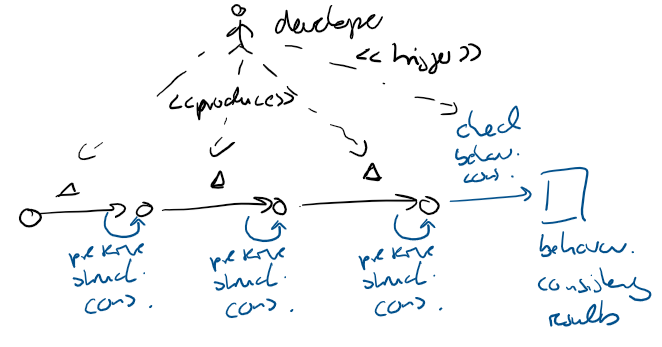
\includegraphics[width=0.8\textwidth]{figures/prologue/networks/process_structure_behavior.png}
    \caption[Process for preserving structural and behavioral consistency]{Proposed process for continuously preserving structural and explicitly checking behavioral consistency}
    \label{fig:networks:process_structure_behavior}
\end{figure}

\mnote{Fine-grained preservation of structural relations}
In consequence, the distinction between structural and behavioral consistency relations is also relevant for the processes of checking and preserving consistency.
While structural consistency relations may be preserved often in a fine-grained way, behavioral consistency relations may be checked less often.
We depict the proposed process in \autoref{fig:networks:process_structure_behavior}.
In the best case, a consistency mechanism can give hints to potential behavioral consistency violations more often.
For example, a performance-relevant modification of the implementation could lead to a hint for the developer that performance may be affected by his modification with the information about the previous analysis result, such that he or she can guess whether his modification will violate the requirement.
Given the information that a response time requirement of 10 milliseconds was fulfilled during the last check by an actual response time of 1 millisecond could help the developer to decide that his modification will not violate that requirement.

\mnote{We focus on structural relations}
In this thesis, we are interested in processes that continuously preserve and not only check consistency.
This is why we explicitly focus on structural consistency relations in this thesis, although the insights might be transferable to behavioral relations as well.
As another consequence, those structural relations that we consider are supposed to be decomposable into binary relations, as discussed in \autoref{chap:networks:notions:types}.



%%
%% CONSISTENCY SPECIFICATION PROCESS
%%
\section{Consistency Specification Process}
\label{chap:networks:specification_process}

\begin{figure}
    \centering
    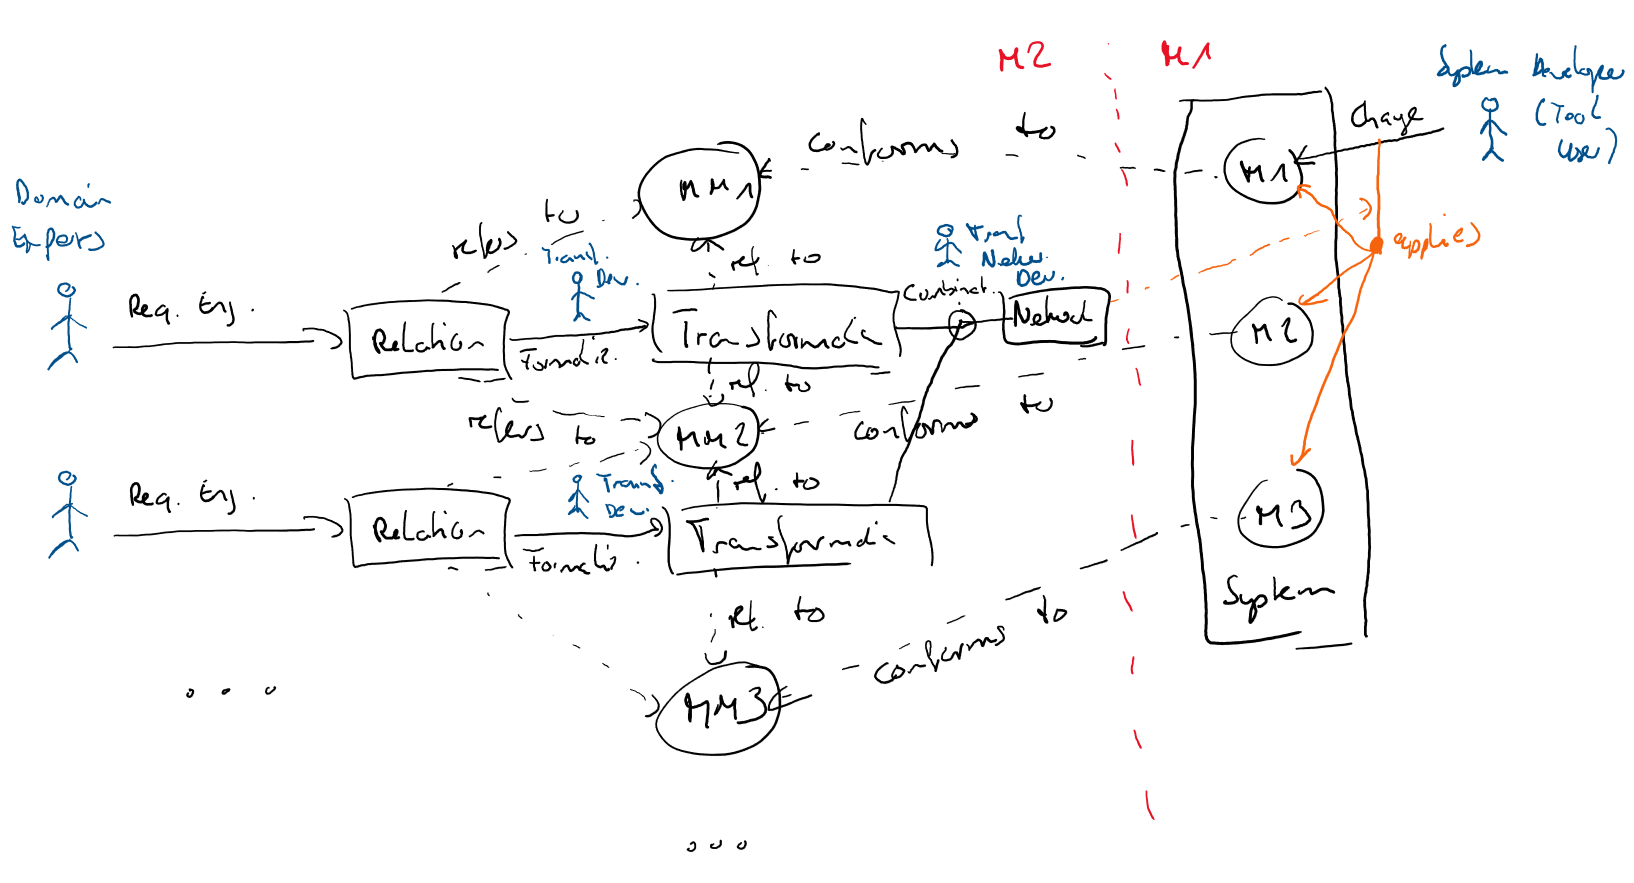
\includegraphics[width=\textwidth]{figures/prologue/networks/roles_and_process}
    \caption[Roles in a transformation network specification process]{Roles involved in a process for specifying a transformation network, their responsibilities and dependencies. Extended from~\owncite{klare2019dagstuhl}.}
    \label{fig:networks:roles_and_process}
\end{figure}

\mnote{Roles and scenarios}
In this thesis, we are concerned with the process of specifying consistency in terms of a transformation network and different problems arising in that process.
We therefore discuss which roles are involved in that process and which different scenarios can be considered that induce requirements and exemplify the application contexts of our later contributions.
\autoref{fig:networks:roles_and_process} gives an overview of the roles and the essential specification process.
While that specification process is concerned with the metamodel level (M2), a transformation network is finally applied at the model level (M1) to a concrete system under development.

\subsection{Roles}

\mnote{Roles in the consistency process}
The specification of a transformation network involves the definition of the individual transformations by \emph{domain experts} and \emph{transformation developers} as well as their combination to a network by \emph{transformation network developers}.
The usage of the network, on the other hand, involves its application to changes to a system under development by a \emph{system developer}, sometimes also called \emph{tool user}~\cite{klare2019dagstuhl}.
Apart from the explicit transformation network, these roles and their responsibilities are comparable to the ones that were defined in a working group of a Dagstuhl seminar, in which the author of this thesis participated~\cite{klare2019dagstuhl}.

\mnote{Roles for the specification}
A domain expert has the knowledge about the consistency relations between two (or more) tools and their languages or, more specifically, the metamodels describing them.
He performs the requirements engineering task for the information to define in a transformation.
A transformation developer is then responsible for formalizing these relations and their preservation in a transformation.
We will usually only refer to the transformation developer, as for us it is not of specific interest where the information about the relations comes from but only that it is encoded into a transformation.
Finally, a transformation network developer combines different transformations, which were usually developed by different transformation developers, to a transformation network.
It may even be possible that several transformation network developers compose several transformation networks to a larger transformation network. 
Whenever the distinction is not relevant, we will refer to both transformation and transformation network developers simply as \emph{transformation developers}.

\mnote{Roles for the usage}
Concrete systems are developed with the use of transformation networks by system developers, who perform changes of models via the tools they use.
Thus, we also call them tool users.
Usually different system developers will be responsible for different models.
In our introductory example, we distinguished between software architects, developers, requirements engineers and so on.
Performing changes leads to the application of the transformation network to restore consistency of the models.
In this thesis, we refer to system developers as \emph{users}, as they are the ones using the transformation networks we are concerned with.

\mnote{Multiple roles fulfillable by same persons}
The roles reflect the different responsibilities when specifying and using transformation networks.
Several of them can, however, be fulfilled by the same persons.
This especially applies to domain experts and transformation developers.
The same person may know about the relations as a domain expert and formalize them in a transformation.
Potentially, a domain expert may even be the one who develops a concrete system as a system developer.


\subsection{Scenarios}

\mnote{Generic and project-specific transformations}
Both for the development of transformations as well as for the combination of transformations to a network, different development scenarios can be distinguished.
Transformations can be developed generically or specific for a project.
\begin{properdescription}
    \item[Generic:] Transformations are developed as artifacts off-the-shelf, which can be used in any project. This especially applies for descriptive transformations (cf. \autoref{chap:networks:notions:normative_descriptive}), which encode a common understanding of consistency, such as for \gls{UML} class models and Java code.
    \item[Project-specific:] Transformations are developed specific for a project. This can occur when a project requires specific rules how elements shall be related. For example, the mapping of components to their realization in the implementation can be specific to the project~\cite{langhammer2017a}. Project-specific transformations can, eventually, later be used in a generic way.
\end{properdescription}

\mnote{Big bang and continuous combination}
The combination of transformations to networks can be distinguished especially regarding the point in time at which the combination takes place.
\begin{properdescription}
    \item[Big bang:] Transformations are developed first and after they have been completed, a transformation network developer combines them to a network. Problems regarding the compatibility of the transformations are first recognized during this combination, thus transformations may need to be adapted afterwards to properly work together.
    \item[Continuous:] Transformations are combined to a network already during their development. Starting with partial or even empty transformations, the structure of the network can be defined early. This allows for a continuous validation of compatibility of the developed transformations. Ultimately, even an online checking of compatibility after each change to a transformation can be performed to get early feedback.
\end{properdescription}

\mnote{Effects of combination process}
For us, it is not relevant whether transformations are developed in a generic or project-specific way.
The distinction of scenarios in which transformation networks are developed is, however, of special interest.
It can be beneficial for transformation developers to get feedback on the compatibility of their developed transformations with others on-the-fly.
This makes locating a problem easier, because only the last changes may have introduced it, whereas with an a-posteriori checking in a big bang process the effort to find compatibility problems may increase because of missing locality.

\mnote{Mixing processes}
While both generic as well as project-specific transformations can be mixed in a single project, also the process of combining them may be mixed.
Some of the transformations may be integrated in a big bang fashion, whereas others are continuously integrated.
This can also be a result of where the transformations come from.
A generic transformation cannot be continuously integrated, because it is not specific for a single project to integrate it into.


%%
%% MODELS AND METAMODELS
%%
\section{Models and Metamodels}
\label{chap:networks:models}

\begin{table}
    \centering
    \small
    \renewcommand{\arraystretch}{1.4}%
    \rowcolors{1}{\secondlinecolor}{\firstlinecolor}
    \begin{tabular}{R{4.8cm} L{5cm}}
        \toprule
        \rowcolor{\headinglinecolor}
        \multicolumn{2}{c}{\textbf{Properties and Classes}}\\
        $P$
            & Property (attribute or reference) \\
        $\instances{P} = \setted{p_1, p_2, \dots}$     
            & Property values of a property $P$ \\
        $\class{C}{} = \tupled{P_1, \dots, P_n}$
            & Class \\
        $\instances{\class{C}{}} = \setted{\object{o}{} = \tupled{p_1, \dots, p_n} \mid p_i \in \instances{P_i}}$ 
            & Instances (objects) of a class $\class{C}{}$\\
        $\object{o}{} \in \instances{\class{C}{}}$
            & Object of a class $\class{C}{}$ \\
        \midrule
        \rowcolor{\headinglinecolor}
        \multicolumn{2}{c}{\textbf{(Meta-)Models}}\\
        $\metamodel{M}{} = \setted{\class{C}{1}, \dots, \class{C}{m}}$
            & Metamodel\\
        $\metamodelinstanceset{M}{} = \setted{\model{m}{} \mid \model{m}{} \subseteq \bigcup_{\class{C}{} \in \metamodel{M}{}} \instances{\class{C}{}}}$
            & Instances of a metamodel\\
        % $\metamodelset{M} = \setted{\metamodel{M}{1}, \dots, \metamodel{M}{k}}$
        %     & Set of metamodels\\
        % $\metamodelsetinstanceset{M} = \setted{ \setted{\model{m}{1}, \dots, \model{m}{k}} \mid \model{m}{i} \in \metamodelinstanceset{M}{i}}$
        %     & Instances of a metamodel set $\metamodelset{M}$\\
        $\metamodeltuple{M} = \tupled{\metamodel{M}{1}, \dots, \metamodel{M}{k}}$
            & Tuple of metamodels\\
        $\metamodeltupleinstanceset{M} = \metamodelinstanceset{M}{1} \times \dots \times \metamodelinstanceset{M}{k} = \setted{ \tupled{\model{m}{1}, \dots, \model{m}{k}} \mid \model{m}{i} \in \metamodelinstanceset{M}{i}}$
            & Instances of a metamodel tuple $\metamodeltuple{M} = \tupled{\metamodel{M}{1}, \dots, \metamodel{M}{k}}$\\
        $\model{m}{} \in \metamodelinstanceset{M}{}$
            & Model of metamodel $\metamodel{M}{}$\\
        $\modeltuple{m} \in \metamodeltupleinstanceset{M}$
            & Model tuple of a metamodel tuple $\metamodeltuple{M}$\\
        \bottomrule
    \end{tabular}
    \caption[Models, metamodels, their elements and notations]{Models, metamodels, their elements and notations}
    \label{tab:networks:elements}
\end{table}

\mnote{Notation overview}
The most essential elements used for descriptions in this thesis are models and the metamodels describing them.
We have already introduced in \autoref{chap:foundations} what we consider a model and that we adhere to the modeling formalism defined by the \gls{MOF}.
We use a sufficiently simplified notion of models, metamodels, and their elements, for which we give an overview in \autoref{tab:networks:elements}.
In the following, we introduce the used notation and its conventions, as well as the elements used for modeling.
Finally, we clarify assumptions that we make and discuss their impact.


\subsection{Notation and Conventions}

\mnote{Modeling levels}
In general, we use variables of uppercase letters for all elements at the metamodel level (M2), such as $\metamodel{M}{}$ for a metamodel or $\class{C}{}$ for a class, whereas we use lowercase letters for all elements at the model level (M1), such as $\model{m}{}$ for a model and $\object{o}{}$ for an object.

\mnote{Notation for model and metamodel level relations}
We use the notations for sets and tuples introduced in \autoref{chap:foundations:notations} for denoting sets and tuples of the different elements, such as metamodels and models.
When considering multiple metamodels or models, we are usually not interested in their order and usually the same model or metamodel cannot appear twice.
Still, we always treat them as tuples rather than sets to be able to easily relate a model to its metamodel by its index within the tuple.
Thus, if not further specified, we use the same indices to relate element at the metamodel and the model level, such as as $\model{m}{1}$ being an instance of $\metamodel{M}{1}$, i.e., $\model{m}{1} \in \metamodelinstanceset{M}{1}$.
This could also be expressed by an explicit instantiation relation, but the used notation is more concise and thus proposes to easy readability.


\subsection{Modeling Elements}

\mnote{Elements overview}
In general, we consider metamodels as a composition of \metaclasses, which, in turn, are composed of properties representing attributes or references.
Models instantiate metamodels and are composed of objects, which are instances of \metaclasses and, in turn, consist of property values, which instantiate properties.

\mnote{Properties and property values}
We denote \emph{properties}, which are the information a \metaclass consists of, such as attributes or references, as $P$ and the \emph{property values} as instances of a property as $\instances{P} = \setted{p_1, p_2, \dots}$ of property $P$. 
We do not need to further differentiate different types of properties into attributes and references, like it is done in other formalizations, such as the \gls{OCL} standard~\cite[A.1]{ocl} or the thesis of \citeauthor{kramer2017a}~\cite[2.3.2]{kramer2017a}.

\mnote{Classes and objects}
We denote \emph{meta-classes}, in the following shortly called \emph{classes}, as tuples of properties $\class{C}{} = \tupled{P_1, \dots, P_n}$. 
Instances of a class are \emph{objects}, each being a tuple of instances of the properties of the class.
We denote all instances of a class $\class{C}{}$ as $\instances{\class{C}{}} = \setted{\object{o}{} = \tupled{p_1, \dots, p_n} \mid p_i \in \instances{P_i}}$.

\mnote{Metamodels and models}
We denote a metamodel $\metamodel{M}{} = \setted{\class{C}{1}, \dots, \class{C}{m}}$ as a finite set of classes.
The instances of a metamodel are sets of objects $\metamodelinstanceset{M}{} = \setted{\model{m}{} \mid \model{m}{} \subseteq \bigcup_{\class{C}{} \in \metamodel{M}{}} \instances{\class{C}{}}}$.
In other work like~\cite{stevens2020BidirectionalTransformationLarge-SoSym}, such instance sets are also called \emph{model sets} and implicitly define a metamodel, thus representing a lightweight definition of metamodels by simply enumerating its instances.
Each instance of a metamodel is called a \emph{model}, and represents a finite set of objects that instantiate the classes in the metamodel.
For a tuple of metamodels $\metamodeltuple{M} = \tupled{\metamodel{M}{1}, \dots, \metamodel{M}{k}}$, we denote the set that contains all sets of instances of that metamodels as $\metamodeltupleinstanceset{M} = \setted{ \tupled{\model{m}{1}, \dots, \model{m}{k}} \mid \model{m}{i} \in \metamodelinstanceset{M}{i}}$.

\mnote{Valid models}
With $\instances{\class{C}{}}$ and $\metamodelinstanceset{M}{}$, we denote the sets of instances of a class and metamodels, i.e., the objects and models instantiating them.
Usually, additional constraints exist that further restrict these sets.
For example, a property can represent a reference to another object, thus if a class contains a specific property value representing a reference to an object, the referenced object must be contained in the model as well.
Thus, the sets of \emph{valid} instances of classes and metamodels are usually only subsets of the sets we denote with $\instances{\class{C}{}}$ and $\metamodelinstanceset{M}{}$, respectively.
For reasons of simplicity, we will, however, usually only refer to the denoted instance sets.
The statements still apply to the sets of valid object and models as subsets of considered sets.

%\todo{Ergänzen, dass wir die Fälle diskutieren, wo sich das nicht übertragen lässt (konkrete Kompatibilität). Dort dann erklären, wie Kombination aus Restriktion auf valide Modelle + Konsistenzrelationen nur gewünsche Modellmengen zulässt. Außerdem diskutieren, warum Kompatibilität nicht auf validen Modellen definiert ist.}

%\todo{Discuss valid models, why we do not consider them and prove that invariants + consistency relations can express any consistency relation.
%A single relation can consider constraints on the single models, but combination (even within one transformation) can easily contradict constraints of a model.
%New:
%Discuss valid models here and why we do not further consider them. Discuss at end of (or somewhere in) compatibility how combination of valid model restriction and consistency relations can express any restriction to desired model sets.}

%\todo{Idee für das Ausschluss-Problem (Für Student darf kein Employee existieren): Entweder darf nie ein entsprechender Employee existieren, dann müssen die Modelle allesamt ausgeschlossen werden (valid models). Wenn es in bestimmten Modellen auftreten darf, muss der Kontext einer Konsistenzrelation richtig festgelegt sein, damit sie abbildet unter welchen Bedingungen der Employee existieren darf. Geht aber nicht, weil Employee einfach in keiner Relation auftauchen könnte (man will nie, dass ein Employee für ein anderes Element vorhanden ist), aber man will, dass er in bestimmten Situationen nicht auftauchen darf.}



\subsection{Assumptions}
\label{chap:networks:models:assumption}

\mnote{Finite models}
We assume models to be finite, so for each model $\model{m}{}$, we assume that $|\model{m}{}| < \infty$.
Additionally, our proposed formalism assumes objects to be unique within a model $\model{m}{}$. 
This is already implicitly covered by the definition of $\metamodelinstanceset{M}{}$ for the instances of a metamodel $\metamodel{M}{}$. 

\mnote{Unique elements}
In practice, it is usually allowed to have the same object, i.e., an element with the same type, attribute and reference values, multiple times within the same model. 
This is, however, only a matter of identity, which, in practice, is given at least by different objects being placed at specific places in memory.
We assume, without loss of generality, the necessary information to distinguish two elements to be represented within properties of these elements.

% Our definition of models does not restrict validity of models apart from being a collection of instances of the classes in the metamodel.
% It is possible to define further constraints for metamodels that restrict their valid instances.
% We intentionally do not consider such restrictions of valid models, because even a single transformation 



%%
%% RUNNING EXAMPLE
%%
\section{Running Example}
\label{chap:networks:example}

%\todo{Address von Resident in "Location" auslagern und Address von "Person" in Address auslagern. Also remove $R'_{ER}$ and move it to compatibility chapter, as it is not yet relevant here.}

\begin{figure}
    \centering
    %% From motivational_example in MPM4CPS paper

\newcommand{\hdistance}{14em}
\newcommand{\classwidth}{6em}

\begin{tikzpicture}

% Person
\umlclassvarwidth{person}{}{Person\sameheight}{
firstname\\
lastname\\
address\\
income
}{\classwidth}

% Employee
\umlclassvarwidth[,above right=2em and \hdistance of person.east, anchor=south]{employee}{}{Employee\sameheight}{
name\\
socsecnumber\\
salary
}{\classwidth}

\umlclassvarwidth[,below=4em of employee.south, anchor=north]{resident}{}{Resident\sameheight}{
name\\
address\\
socsecnumber
}{\classwidth}


% CONSISTENCY RELATIONS
\draw[consistency relation] (person.north) |- node[pos=0, above left] {$p$} node[pos=0.75, above] {$\consistencyrelation{CR}{PE}$} node[pos=1, above left] {$e$} (employee.west);
\draw[consistency relation] (employee.south) -- node[pos=0, below left] {$e$} node[right, align=left] {$\consistencyrelation{CR}{ER}$}% /\\ $R'_{ER}$} 
node[pos=1, above left] {$r$} (resident.north);
\draw[consistency relation] (resident.west) -| node[pos=0, below left] {$r$} node[pos=0.25, below] {$\consistencyrelation{CR}{PR}$} node[pos=1, below left] {$p$} (person.south);

\draw[consistency relation 2] (person.east) -- node[pos=0, below right] {$p$} ++(0.35*\hdistance,0) -- node[pos=0, above=0.5em] {$\consistencyrelation{CR}{PER}$} node[pos=1, above left] {$e$} ([yshift=1em]employee.south west);
\draw[consistency relation 2, -latex] ([xshift=0.35*\hdistance]person.east) -- node[pos=1, below left] {$r$} ([yshift=-1em]resident.north west);

\node[consistency related element 2, below left=5em and 2em of person.south west, anchor=north west, inner sep=0em] (relations1) {
$\begin{aligned}
    \consistencyrelation{CR}{PER} =\; &
            \setted{\tupled{p,e,r} \mid 
            %& 
            \mathvariable{p.firstname} + \text{\enquote{\textvisiblespace}} + \mathvariable{p.lastname} = \mathvariable{e.name} = \mathvariable{r.name} \\
            &
            \land \mathvariable{p.address} = \mathvariable{r.address}
            \land \mathvariable{p.income} = \mathvariable{e.salary} \\
            &
            \land \mathvariable{e.socsecnumber} = \mathvariable{r.socsecnumber}
        }
\end{aligned}$
};

\node[consistency related element, below=0.5em of relations1.south west, anchor=north west, inner sep=0em] {
$\begin{aligned}
    \consistencyrelation{CR}{PE} =\; &
            \setted{\tupled{p,e} \mid %\\
            %& 
            \mathvariable{p.firstname} + \text{\enquote{\textvisiblespace}} + \mathvariable{p.lastname} = \mathvariable{e.name}%\\
            %& 
            \land \mathvariable{p.income} = \mathvariable{e.salary}
        }\\[0.3em]
        \consistencyrelation{CR}{PR} =\; &
            \setted{\tupled{p,r} \mid %\\
            %& 
            \mathvariable{p.firstname} + \text{\enquote{\textvisiblespace}} + \mathvariable{p.lastname} = \mathvariable{r.name}%\\
            %& 
            \land \mathvariable{p.address} = \mathvariable{r.address}
        }\\[0.3em]
        \consistencyrelation{CR}{ER} =\; &
            \setted{\tupled{e,r} \mid %\\
            %& 
            \mathvariable{e.name} = \mathvariable{r.name} %\\
            %& 
            \land \mathvariable{e.socsecnumber} = \mathvariable{r.socsecnumber}
        }%\\
    % R'_{ER} =\; &
    %         \setted{\tupled{e,r} \mid %\\
    %         %& 
    %         e.name.toLower = r.name\\
    %         & \land e.socsecnumber = r.socsecnumber
    %     }
\end{aligned}$
};

\end{tikzpicture}
    \caption[Three metamodels with exemplary consistency relations]{Three simple metamodels for persons, employees and residents. One ternary relation $\consistencyrelation{CR}{PRE}$ between them and three binary relations $\consistencyrelation{CR}{PE}, \consistencyrelation{CR}{PR}, \consistencyrelation{CR}{ER}$ between each pair of them describing consistency.}
    \label{fig:networks:three_persons_example}
\end{figure}

\mnote{Metamodels}
We use different variations of a running example throughout several parts of this thesis.
The basic example is depicted in \autoref{fig:networks:three_persons_example}.
It contains three metamodels, one with persons, one with employees and one with residents, each containing the name and some information specific for that metamodel.
Although these metamodels are rather simple and do not cover metamodels from the software engineering domain, they are sufficient to explain the concepts in this thesis and are easy to comprehend.

\mnote{Consistency relations}
The example also contains a description of consistency between these three metamodels, although only informally given at this point and more precisely defined later on.
It requires that if any person, employee or resident is contained in a model, there must also be the other two elements with the same names, addresses, incomes and social security numbers.
Like for the metamodels themselves, it can be challenged whether this consistency relation may be reasonable, but it is easy to comprehend and sufficient for explaining the essential concepts and also several issues in this thesis.
This relation can either be expressed as a ternary relation, denoted as $\consistencyrelation{CR}{PER}$, or as three binary relations $\consistencyrelation{CR}{PE}, \consistencyrelation{CR}{PR}, \consistencyrelation{CR}{ER}$.
Three models fulfill the ternary relation in exactly those cases in which each pair fulfills the according binary relation.
The relations consist of tuples of the elements that are considered consistent, i.e., the pairs or triples of elements with the specified relation of their property values.

\mnote{Equivalence of consistency relations}
The metamodels and consistency relations are defined in a way such that no pair of the three binary consistency relations is equivalent to the ternary relation, in the sense that the same models are considered consistent to these two binary relations whenever they are considered consistent to the ternary relation.
This is a consequence of each pair of metamodels sharing some unique information, which is the income, the salary and the social security number.
In consequence, we cannot omit one of the binary relations without loosing consistency guarantees compared to the ternary relation.



% \begin{copiedFrom}{ICMT}
    
% % EXEMPLARY PROBLEMS
% Consider the simple consistency relations exemplified in \autoref{fig:properties:motivational_example}.
% A company uses three software systems to manage (1)~personnel data, (2)~tasks and their assignment to employees, and (3)~schedules for work times of employees and the deadlines of tasks.
% The domain models contain dependent information, especially the data about employees and their relations to tasks, but none of them contains a superset of information of another, which requires to define consistency between all pairs of them.
% If three domain experts define %the consistency constraints between all pairs of the metamodels 
% those binary constraints
% independently, they can easily contradict. 
% For example, imagine %that they specify 
% a direct mapping of employee \emph{name} representations between the task management and scheduling system, a concatenation of \emph{firstname} and \emph{lastname} between personnel data and task management system and a comma-separated concatenation of \emph{lastname} and \emph{firstname} between personnel data and scheduling system.
% These constraints are obviously incompatible, as they cannot be fulfilled at the same time.
% %Additionally, even if the name mappings were compatible, specifying three transformations between all pairs of metamodels that preserve those constraints leads to redundancies within the transformations.
% %In consequence, the transformation have to ensure that they no element duplications arise from that.
% %%leads to redundant the operationalization of transformations that preserve these constraints has to ensure that no element duplications arise from redundant transformations paths. 
% %%Additionally, even if the name mapping was compatible, the operationalization of transformations that preserve these constraints has to ensure that no element duplications arise from redundant transformations paths. 
% %For example, after adding an employee to the personnel data system, a transformation adds an employee to the task management system, which is then transformed into an employee in the scheduling system. 
% %The additional transformation between personnel and scheduling system must correctly consider that an employee was already created transitively.
% %\todoHeiko{Checken, ob auf Duplizierungsproblem später verwiesen wird, dann hier wieder einfügen}

% \begin{figure}[tb]
%     \centering
%     %\includegraphics[angle=270, width=\textwidth]{figures/motivation_employee_example.pdf}
%     \newcommand{\hdistance}{10.5em}
\newcommand{\classwidth}{4.5em}
\newcommand{\sameheight}{\vphantom{Êy}}

\begin{tikzpicture}

% \node[uml class] (personal_employee) {Employee
% \nodepart{two}
% name\\
% address\\
% salary\\
% dailyWorkingTime\\
% department
% };

% PERSONNEL
\umlclassvarwidth{personnel_employee}{}{Employee\sameheight}{
firstname\\
lastname\\
%address\\
salary\\
workingTime\\
department
}{\classwidth}

\node[above=0.2em of personnel_employee.north] (personnel_label) {\small \emph{(1) Personnel Data}};


% TASK MANAGEMENT
\umlclassvarwidth[,right=\hdistance of personnel_employee.north, anchor=north]{task_task}{}{Task\sameheight}{
name\\
description\\
%department
}{\classwidth}

\umlclassvarwidth[,below=1.5em of task_task.south, anchor=north]{task_employee}{}{Employee\sameheight}{
name\\
department
}{\classwidth}

\umlassociationfromto{(task_employee) -- %node[uml role end] {assigned to} 
node[uml cardinality end, pos=0.7, left] {*} node[uml role end, pos=0.65, right] {responsible for}  node[uml cardinality start, pos=0.2, left] {*} (task_task)}

\node[above=0.2em of task_task.north] (task_label) {\small \emph{(2) Task Management}};


% SCHEDULING
\umlclassvarwidth[,right=\hdistance of task_task.north, anchor=north]{scheduling_task}{}{Task\sameheight}{
name\\
deadline
}{\classwidth}

\umlclassvarwidth[,right=8.5em of scheduling_task.north, anchor=north]{scheduling_schedule}{}{Schedule\sameheight}{}{\classwidth}

\umlclassvarwidth[,below=1.5em of scheduling_schedule.south, anchor=north]{scheduling_workday}{}{WorkDay\sameheight}{
date
}{\classwidth}

\umlclassvarwidth[,right=\hdistance of task_employee.north, anchor=north]{scheduling_employee}{}{Employee\sameheight}{
name\\
workingTime
}{\classwidth}

\umlcomposition{(scheduling_schedule) -- node[uml cardinality end] {*} (scheduling_schedule-|scheduling_task.east)}
\umlcomposition{(scheduling_schedule) -- node[uml cardinality end] {*} (scheduling_workday)}
\umlassociationfromto{([yshift=-0.5em]scheduling_workday.west) -- node[uml cardinality end] {*} node[uml role end, above, pos=0.5] {working} ([yshift=-0.5em]scheduling_workday.west-|scheduling_employee.east)}
\umlassociationfromto{(scheduling_employee) -- node[uml cardinality start, pos=0.2, right] {*} node[uml cardinality end, pos=0.7, right] {*} node[uml role end, left, pos=0.6] {responsible for} (scheduling_task)}

\coordinate (scheduling_upper_middle) at ($(scheduling_schedule.north)!0.5!(scheduling_task.north)$);
\node[above=0.2em of scheduling_upper_middle] (scheduling_label) {\small \emph{(3) Scheduling}};


% CONSISTENCY RELATIONS
\draw[consistencyrel] ([xshift=0.5em]personnel_employee) |- node[pos=0.75, below, align=center] {(first/last)name,\\ department} ([yshift=-2.2em]task_employee.north west);
\draw[consistencyrel] ([yshift=-2.2em]task_employee.north east) -- node[below, align=center] {name, \\ relation to task} ([yshift=-2.2em]scheduling_employee.north west);
\draw[consistencyrel] ([xshift=-0.5em]personnel_employee.south) -- ++(0,-4.2em) -| node[above, pos=0.25] {(first/last)name, workingTime} (scheduling_employee.south);
\draw[consistencyrel] (task_task.east) -- node[below] {name} (task_task.east-|scheduling_task.west);

\end{tikzpicture}
%     %\caption{Exemplary Consistency Relations between a PCM, UML Class and Java Model}
%     \caption{Exemplary Consistency Relations ({\protect\tikz[baseline=-0.5ex] \protect\draw[latex-latex, consistency related element] (0,0) -- (1.5em,0);}) between Three Simple Metamodels} %Personnel, Task Management and Scheduling System Metamodels}
%     \label{fig:properties:motivational_example}
% \end{figure}

% % ABSTRACT PROBLEMS
% While such a problem may be trivially solvable in this simple scenario, it gets difficult in systems with more and larger metamodels, %, especially in software development or system engineering scenarios, in which 
% where
% each domain expert only knows about the relation between two of them, but not about the others.
% In consequence, each \ac{BX} has to be constructed in such a way that it can be combined with other, independently developed \acp{BX} in a \emph{black-box} manner later on.
% Issues that arise from such a combination of independently developed \acp{BX} %the combination of independently developed \acp{BX} %to networks of them 
% have not been investigated yet. %and categorized yet.
% In consequence, potential failures, causal mistakes and techniques to avoid them by design are not systematically known.

% \end{copiedFrom} % ICMT


\part{Classifying Transformation Networks 
    \pgsize{40 p.}
}

%% Goal is to find out, what makes transformation networks out, what are their properties, impacts of topologies, processes to build them and so on

%% Use a coarse-grained notion of consistency here. It's precised in the correctness part.

\chapter{Consistency Specification Levels
    \pgsize{15 p.}
}

\begin{copiedFrom}{ICMT}

% CONTEXT - MOTIVATION FOR NETWORKS OF BX
Models that contain concern-specific extracts of a system are a means to deal with the increasing complexity in today's software development. % projects. % of today's software systems.
%The complexity of software systems is continuously increasing.
%One approach to deal with that is the separation of a system description into different models containing concern-specific properties or extracts of the system.
%Such a fragmentation of information %into different models 
%results in dependencies %and redundancies 
%that have to be kept consistent.
%A common approach for preserving consistency between models are transformations, which incrementally update the models to stay consistent.
%\emph{Incremental \acp{BX}}, which keep two types of models consistent, are well researched. %, especially in terms of \emph{bidirectional transformations}, which consider both directions of changes.
A common approach for preserving consistency between %dependent information in 
such models are incremental \acp{BX}, which %incrementally 
keep two types of models consistent.
Usually, more than two types of models are used in development processes. % within a project. %development process. %, which necessitates approaches that keep multiple models consistent.
% ABSTRACT PROBLEMS
%\todoHeiko{Obsolete?}
%Consistency between multiple types of models 
Keeping them consistent can be achieved by combining \acp{BX} to networks, which has not been focused in research yet~\cite{stevens2017a}.
When such networks contain cycles, %is not a tree anymore, problems can easily occur, because 
information can be propagated across different paths during transformation execution, which may lead to problems on confluence.
%Those problems can occur because of different reasons.
%One reason is that the individual transformations are developed independently by different domain experts, who do usually not know about the transformations their one will be combined with.
%This can easily lead to contradictions in the considered consistency relations, as well as their operationalization.
%This is especially problematic if different domain experts only know about consistency relations within a limited set of models.
%They develop transformations independently, without knowing about the other transformations their one will be combined with later on.
%Such a \emph{black-box} combination can easily lead to contradictions in the considered consistency constraints as well as incompatibilities of thee operationalization of combined transformations.

%Consider the consistency relations exemplified on three simple models in \autoref{fig:motivation_example}.
%The \ac{PCM} is a component-based architecture description language, which also provides abstract specifications of services, so called SEFFs, to conduct performance predictions~\cite{reussner2016a}.
%A component is represented as one implementation class and one utility class in UML and Java code.
%SEFFs are represented as methods.
%These consistency relations are an alternation of those developed by \cite{langhammer2015a}.

% EXEMPLARY PROBLEMS
Consider the simple consistency relations exemplified in \autoref{fig:properties:motivational_example}.
A company uses three software systems to manage (1)~personnel data, (2)~tasks and their assignment to employees, and (3)~schedules for work times of employees and the deadlines of tasks.
The domain models contain dependent information, especially the data about employees and their relations to tasks, but none of them contains a superset of information of another, which requires to define consistency between all pairs of them.
If three domain experts define %the consistency constraints between all pairs of the metamodels 
those binary constraints
independently, they can easily contradict. 
For example, imagine %that they specify 
a direct mapping of employee \emph{name} representations between the task management and scheduling system, a concatenation of \emph{firstname} and \emph{lastname} between personnel data and task management system and a comma-separated concatenation of \emph{lastname} and \emph{firstname} between personnel data and scheduling system.
These constraints are obviously incompatible, as they cannot be fulfilled at the same time.
%Additionally, even if the name mappings were compatible, specifying three transformations between all pairs of metamodels that preserve those constraints leads to redundancies within the transformations.
%In consequence, the transformation have to ensure that they no element duplications arise from that.
%%leads to redundant the operationalization of transformations that preserve these constraints has to ensure that no element duplications arise from redundant transformations paths. 
%%Additionally, even if the name mapping was compatible, the operationalization of transformations that preserve these constraints has to ensure that no element duplications arise from redundant transformations paths. 
%For example, after adding an employee to the personnel data system, a transformation adds an employee to the task management system, which is then transformed into an employee in the scheduling system. 
%The additional transformation between personnel and scheduling system must correctly consider that an employee was already created transitively.
%\todoHeiko{Checken, ob auf Duplizierungsproblem später verwiesen wird, dann hier wieder einfügen}

\begin{figure}[tb]
    \centering
    %\includegraphics[angle=270, width=\textwidth]{figures/motivation_employee_example.pdf}
    \newcommand{\hdistance}{10.5em}
\newcommand{\classwidth}{4.5em}
\newcommand{\sameheight}{\vphantom{Êy}}

\begin{tikzpicture}

% \node[uml class] (personal_employee) {Employee
% \nodepart{two}
% name\\
% address\\
% salary\\
% dailyWorkingTime\\
% department
% };

% PERSONNEL
\umlclassvarwidth{personnel_employee}{}{Employee\sameheight}{
firstname\\
lastname\\
%address\\
salary\\
workingTime\\
department
}{\classwidth}

\node[above=0.2em of personnel_employee.north] (personnel_label) {\small \emph{(1) Personnel Data}};


% TASK MANAGEMENT
\umlclassvarwidth[,right=\hdistance of personnel_employee.north, anchor=north]{task_task}{}{Task\sameheight}{
name\\
description\\
%department
}{\classwidth}

\umlclassvarwidth[,below=1.5em of task_task.south, anchor=north]{task_employee}{}{Employee\sameheight}{
name\\
department
}{\classwidth}

\umlassociationfromto{(task_employee) -- %node[uml role end] {assigned to} 
node[uml cardinality end, pos=0.7, left] {*} node[uml role end, pos=0.65, right] {responsible for}  node[uml cardinality start, pos=0.2, left] {*} (task_task)}

\node[above=0.2em of task_task.north] (task_label) {\small \emph{(2) Task Management}};


% SCHEDULING
\umlclassvarwidth[,right=\hdistance of task_task.north, anchor=north]{scheduling_task}{}{Task\sameheight}{
name\\
deadline
}{\classwidth}

\umlclassvarwidth[,right=8.5em of scheduling_task.north, anchor=north]{scheduling_schedule}{}{Schedule\sameheight}{}{\classwidth}

\umlclassvarwidth[,below=1.5em of scheduling_schedule.south, anchor=north]{scheduling_workday}{}{WorkDay\sameheight}{
date
}{\classwidth}

\umlclassvarwidth[,right=\hdistance of task_employee.north, anchor=north]{scheduling_employee}{}{Employee\sameheight}{
name\\
workingTime
}{\classwidth}

\umlcomposition{(scheduling_schedule) -- node[uml cardinality end] {*} (scheduling_schedule-|scheduling_task.east)}
\umlcomposition{(scheduling_schedule) -- node[uml cardinality end] {*} (scheduling_workday)}
\umlassociationfromto{([yshift=-0.5em]scheduling_workday.west) -- node[uml cardinality end] {*} node[uml role end, above, pos=0.5] {working} ([yshift=-0.5em]scheduling_workday.west-|scheduling_employee.east)}
\umlassociationfromto{(scheduling_employee) -- node[uml cardinality start, pos=0.2, right] {*} node[uml cardinality end, pos=0.7, right] {*} node[uml role end, left, pos=0.6] {responsible for} (scheduling_task)}

\coordinate (scheduling_upper_middle) at ($(scheduling_schedule.north)!0.5!(scheduling_task.north)$);
\node[above=0.2em of scheduling_upper_middle] (scheduling_label) {\small \emph{(3) Scheduling}};


% CONSISTENCY RELATIONS
\draw[consistencyrel] ([xshift=0.5em]personnel_employee) |- node[pos=0.75, below, align=center] {(first/last)name,\\ department} ([yshift=-2.2em]task_employee.north west);
\draw[consistencyrel] ([yshift=-2.2em]task_employee.north east) -- node[below, align=center] {name, \\ relation to task} ([yshift=-2.2em]scheduling_employee.north west);
\draw[consistencyrel] ([xshift=-0.5em]personnel_employee.south) -- ++(0,-4.2em) -| node[above, pos=0.25] {(first/last)name, workingTime} (scheduling_employee.south);
\draw[consistencyrel] (task_task.east) -- node[below] {name} (task_task.east-|scheduling_task.west);

\end{tikzpicture}
    %\caption{Exemplary Consistency Relations between a PCM, UML Class and Java Model}
    \caption{Exemplary Consistency Relations ({\protect\tikz[baseline=-0.5ex] \protect\draw[latex-latex, consistency related element] (0,0) -- (1.5em,0);}) between Three Simple Metamodels} %Personnel, Task Management and Scheduling System Metamodels}
    \label{fig:properties:motivational_example}
\end{figure}

% ABSTRACT PROBLEMS
While such a problem may be trivially solvable in this simple scenario, it gets difficult in systems with more and larger metamodels, %, especially in software development or system engineering scenarios, in which 
where
each domain expert only knows about the relation between two of them, but not about the others.
In consequence, each \ac{BX} has to be constructed in such a way that it can be combined with other, independently developed \acp{BX} in a \emph{black-box} manner later on.
Issues that arise from such a combination of independently developed \acp{BX} %the combination of independently developed \acp{BX} %to networks of them 
have not been investigated yet. %and categorized yet.
In consequence, potential failures, causal mistakes and techniques to avoid them by design are not systematically known.

% GOAL AND CONTRIBUTIONS
Our research goal is to identify and categorize issues that can arise from the combination of independently developed \acp{BX} to networks and how those issues can be avoided by construction. 
%Instead of performing analysis a-posteriori, when combining transformations to a network, we investigate how to deal with issues a-priori by avoiding them.
Our main contributions in this paper are:
\begin{description}[leftmargin=\parindent]
    \item[\contributionlabel{contrib:levels}{Classification of consistency specification levels}{C1}:] We identify different conceptual levels at which consistency for a set of model types can be defined.
    \item[\contributionlabel{contrib:issues}{Categorization of interoperability issues}{C2}:] We identify potential failures and mistakes in transformation networks and relate them to the specification levels.
    \item[\contributionlabel{contrib:avoidance}{Issue avoidance strategies}{C3}:] We discuss avoidance strategies for mistakes at the different levels and their degree of independence from the concrete scenario. %develop a problem-independent strategy to avoid a category of issues on one specification level.
    \item[\contributionlabel{contrib:evaluation}{Appropriateness evaluation}{C4}:] We show completeness and appropriateness of our categorization by applying it to %a case study of 
    independently developed transformations. %We apply our categorization %and the solution strategy 
    %to a case study of independently developed transformations to show completeness and appropriateness . %of our categorization.
\end{description}

We want to achieve a development process in which 
%that 
\acp{BX} are specified as partial descriptions of consistency, %in a complete system 
which can be combined to a network on demand, so that their repeated execution in arbitrary order leads to a consistent state after changes.
Our contributions help to achieve that by forming systematic knowledge on interoperability issues that have to be considered and solved.
%\todoHeiko{Add benefit of these contributions}

%We start with a clarification of assumptions and a formalization of basic concepts in \autoref{sec:foundations}.
%\autoref{sec:process} defines three conceptual levels in the consistency specification process.
%In \autoref{sec:classification}, we identify and categorize issues in transformation networks.
%We develop a solution strategy for one category of issues in \autoref{sec:avoiding} and evaluate our findings in \autoref{sec:evaluation}.
%After a comparison with related work in \autoref{sec:relatedwork}, we conclude the paper.


% Problem:
% \begin{itemize}
%     \item bx good for keeping models incrementally consistency
%     \item Usually more than two models involved
%     \item bx can be chained but as soon as the network is not a tree anymore, problems can easily occur
%     \item Additionally: Usually each domain expert develops single bx, which has to be combined with others afterwards, without knowing about them a priori (make this really, really clear as an important assumption!)
%     \item Such interoperability issues of incremental bx were not systematically investigated
% \end{itemize}

% \todoHeiko{Make assumptions explicit! Incremental, distributed development (divide and conquer), ...}
% \begin{itemize}
%     \item Repair, not only checking!
%     \item Incremental transformations for consistency preservation
%     \item Independent development of binary transformations by domain experts -> Necessity to independently develop and combine transformations afterwards
%     \item Normative: We define what is consistent (rather than defining consistency and checking it against a "real" relation)
% \end{itemize}

% Goal:
% \begin{itemize}
%     \item Goal was to investigate, how far interoperability of transformations can be achieved by construction (a-priori, rather than a-posteriori analysis)
%     \item Therefore, we categorized specification levels, mistakes and resulting failures associated with the different specification levels to derive from the characteristics of those levels how far they mistakes from that level can be omitted by construction
% \end{itemize}

% MAIN GOAL: Achieve interoperability by construction, as far as possible, by identifying and categorizing potential issues.

% Contribution:
% \begin{enumerate}
%     \item Identification and classification of potential issues $\rightarrow$ catalog to make developers aware of potential faults, their impact/manifestations to know what to consider during development
%     \item Generic solutions for one class of issues that can be generically solved
%     \item Application of classification and solutions to a case study to show completeness, appropriateness
% \end{enumerate}


\section{The Consistency Specification Process}
\todo{Move Specification Levels to top level and remove this somehow}
%\todoHeiko{Annahme: Immer nur Änderung an einem Modell (keine Synchronisation)}

The process of specifying consistency between $n>2$ types of models using a network of \acp{BX} can be separated into different conceptual levels.
We distinguish three such levels:
At the \emph{global level}, we describe the ($n$-ary) relations between all involved model types.
At the \emph{modularization level}, we split these global relations into modular, binary relations.
Finally, at the \emph{operationalization level}, we define preservation of consistency %after changes 
according to the modular relations.
That classification forms our contribution \ref{contrib:levels}.

All of these levels have to be considered during the consistency specification process.
A developer specifies consistency on one of these levels, depending on the abstraction level that the transformation language provides, and the transformation engine finally derives an operationalization from that.
Although a developer does not specify consistency on multiple levels, he or she has to think about the levels on and above the one consistency is specified on.
For example, to define an operationalization, the developer must be aware of the modular consistency relations.
%If a developer only specifies the modular consistency relations, the transformations engine has to derive an appropriate operationalization.
%In the end, to preserve consistency, an operationlization has to be derived from a specification on any of those levels.
The benefit of clearly separating these levels is that they have different potentials for mistakes, faults, and resulting failures. 
Consequently, avoiding a specific kind of mistake, which is related to one of the identified levels, completely prevents a specific category of failures.
We exemplify these levels in \autoref{fig:properties:levels_overview} and explain them in more detail in the following.

%\todoHeiko{Give an example for mistakes here! Maybe one example for every level as well?}

\subsection{Consistency Specification Levels}
\label{chap:properties:levels}

\begin{figure}
    \centering
%    \includegraphics[angle=-90, width=\textwidth]{figures/levels_overview.pdf}
    \newcommand{\modeltypesize}{3.6em}
\newcommand{\modelsize}{0.3em}

\begin{tikzpicture}[
    model type/.style={draw, circle, minimum width=\modeltypesize},
    model/.style={draw, fill, circle, minimum width=\modelsize, inner sep=0},
    label distance=-0.2em,
    every label/.append style={font=\small},
    legend/.style={font=\footnotesize},
    mininode/.style={inner sep=.25em},
]

\foreach \level in {1,2,3} {
    \node[model type, label=265:{$\mathcal{M}_1$}] at (\level*3.45*\modeltypesize, 0) (L\level_MM1) {};
    \node[model, above left=0.25*\modeltypesize and 0.2*\modeltypesize of L\level_MM1.center, anchor=center] (L\level_MM1_M1) {};
    \node[model, right=0.3*\modeltypesize of L\level_MM1.center, anchor=center] (L\level_MM1_M2) {};
    \node[model, below left=0.25*\modeltypesize and 0.2*\modeltypesize of L\level_MM1.center, anchor=center] (L\level_MM1_M3) {};
    
    \node[model type, label=280:{$\mathcal{M}_2$}] at (\level*3.45*\modeltypesize+1.7*\modeltypesize, 0) (L\level_MM2) {};
    \node[model, above right=0.25*\modeltypesize and 0.2*\modeltypesize of L\level_MM2.center, anchor=center] (L\level_MM2_M1) {};
    \node[model, left=0.3*\modeltypesize of L\level_MM2.center, anchor=center] (L\level_MM2_M2) {};
    \node[model, below right=0.25*\modeltypesize and 0.2*\modeltypesize of L\level_MM2.center, anchor=center] (L\level_MM2_M3) {};
    
    \node[model type, label=190:{$\mathcal{M}_3$}] at (\level*3.45*\modeltypesize+0.85*\modeltypesize, -1.35*\modeltypesize) (L\level_MM3) {};
    \node[model, above=0.25*\modeltypesize of L\level_MM3.center, anchor=center] (L\level_MM3_M1) {};
    \node[model, below left=0.25*\modeltypesize and 0.1*\modeltypesize of L\level_MM3.center, anchor=center] (L\level_MM3_M2) {};
    \node[model, below right=0.05*\modeltypesize and 0.25*\modeltypesize of L\level_MM3.center, anchor=center] (L\level_MM3_M3) {};
}

% CONSISTENCY L1
\draw[consistency relation] (L1_MM1_M1) -- (L1_MM2_M1);
\draw[consistency relation] ($(L1_MM1_M1)!0.13!(L1_MM2_M1)$) -- (L1_MM3_M2);
\draw[consistency relation] (L1_MM1_M2) -- (L1_MM2_M2);
\draw[consistency relation] ($(L1_MM1_M2)!0.5!(L1_MM2_M2)$) -- (L1_MM3_M1);

% CONSISTENCY L2
\draw[consistency relation] (L2_MM1_M1) -- (L2_MM2_M1);
\draw[consistency relation] (L2_MM1_M1) -- (L2_MM3_M2);
\draw[consistency relation] (L2_MM2_M1) -- (L2_MM3_M2);
\draw[consistency relation] (L2_MM1_M2) -- (L2_MM2_M2);
\draw[consistency relation] (L2_MM1_M2) -- (L2_MM3_M1);
\draw[consistency relation] (L2_MM2_M2) -- (L2_MM3_M1);

% CONSISTENCY L3
%\draw[consistency relation] (L3_MM1_M1) -- (L3_MM2_M1);
%\draw[consistency relation] (L3_MM1_M1) -- (L3_MM3_M2);
%\draw[consistency relation] (L3_MM2_M1) -- (L3_MM3_M2);
%\draw[consistency relation] (L3_MM1_M2) -- (L3_MM2_M2);
%\draw[consistency relation] (L3_MM1_M2) -- (L3_MM3_M1);
%\draw[consistency relation] (L3_MM2_M2) -- (L3_MM3_M1);

% USER CHANGE L3
\node[model, user changed element, above left=0.25*\modeltypesize and 0.2*\modeltypesize of L3_MM1.center, anchor=center] (L3_MM1_M1) {};
\node[model, user changed element, above right=0.25*\modeltypesize and 0.2*\modeltypesize of L3_MM2.center, anchor=center] (L3_MM2_M1) {};
\node[model, user changed element, below left=0.25*\modeltypesize and 0.1*\modeltypesize of L3_MM3.center, anchor=center] (L3_MM3_M2) {};
\draw[-latex, user changed element] (L3_MM1_M1) -- node[legend, above=0.2em] {$\Delta$} (L3_MM1_M2);

% CONSISTENCY PRESERVATION L3
\node[model, consistency changed element, right=0.3*\modeltypesize of L3_MM1.center, anchor=center] (L3_MM1_M2) {};
\node[model, consistency changed element, left=0.3*\modeltypesize of L3_MM2.center, anchor=center] (L3_MM2_M2) {};
\node[model, consistency changed element, above=0.25*\modeltypesize of L3_MM3.center, anchor=center] (L3_MM3_M1) {};
\draw[-latex, consistency changed element] (L3_MM2_M1) -- node[legend, below right=-0.3em] {$\Delta$} (L3_MM2_M2);
\draw[-latex, consistency changed element] (L3_MM3_M2) -- node[legend, below right=0 and -0.3em] {$\Delta$} (L3_MM3_M1);
\draw[-latex, dashed, consistency changed element, thin] ($(L3_MM1_M1)!0.4!(L3_MM1_M2)$) to[bend left=15] node[legend, above] {$\mathit{CPS}_{\mathit{CS}_{1,2}}$} ($(L3_MM2_M1)!0.4!(L3_MM2_M2)$);
\draw[-latex, dashed, consistency changed element, very thin] ($(L3_MM1_M1)!0.4!(L3_MM1_M2)$) to[bend right=15] node[legend, below left=0.5em and -0.5em] {$\mathit{CPS}_{\mathit{CS}_{1,3}}$} ($(L3_MM3_M2)!0.4!(L3_MM3_M1)$);

% CS LABELS
\node[consistency related element, above left=1.5em and -0.1em of L1_MM3.north, anchor=east, font=\footnotesize] {$\mathit{CS}$};
\node[consistency related element, above left=0.1em and 1.6em of L2_MM3, anchor=center, font=\footnotesize] {$\mathit{CS}_{1,3}$};
\node[consistency related element, above right=0.4em and 1.2em of L2_MM3, anchor=center, font=\footnotesize] {$\mathit{CS}_{2,3}$};
\node[consistency related element, above right=0.8em and 0.25*\modeltypesize of L2_MM1.east, anchor=south, font=\footnotesize] {$\mathit{CS}_{1,2}$};
%\node[consistency related element, above left=0.4em and 1.8em of L3_MM3, anchor=center, font=\footnotesize] {$CS_{1,3}$};
%\node[consistency related element, above right=0.4em and 1.4em of L3_MM3, anchor=center, font=\footnotesize] {$CS_{2,3}$};
%\node[consistency related element, above right=0.8em and 0.25*\modeltypesize of L3_MM1.east, anchor=south, font=\footnotesize] {$CS_{1,2}$};

% LEVEL LABELS
\node[anchor=north] (level1_label) at ([yshift=1.15*\modeltypesize]$(L1_MM1)!0.5!(L1_MM2)$) {Level 1: \emph{Global}};
\node[anchor=north] (level2_label) at ([yshift=1.15*\modeltypesize]$(L2_MM1)!0.5!(L2_MM2)$) {Level 2: \emph{Modularization}};
\node[anchor=north] (level3_label) at ([yshift=1.15*\modeltypesize]$(L3_MM1)!0.5!(L3_MM2)$) {Level 3: \emph{Operationalization}};

\coordinate (legend_anchor) at ([yshift=-0.2*\modeltypesize]L2_MM3.south);

\node[matrix, left=-0.2em of legend_anchor, anchor=north east, outer sep=0em, column sep=0.15em, row sep=-0.4em] (legend_left) {
    \node[model, anchor=center] (model_legend) {}; &
    \node[legend, anchor=west] {model of model type $\mathcal{M}_x$}; \\
    %
    \node[model, user changed element, anchor=center] (user_changed_model_legend)  {}; &
    \node[legend, anchor=west] {consistent models before user change}; \\
    %
    \node[model, consistency changed element, anchor=center] (consistency_preserved_model_legend)  {}; &
    \node[legend, anchor=west] {consistent models after consistency preservation}; \\
};

\node[matrix, left=0.2em of legend_anchor, anchor=north west, column sep=0.15em, row sep=-0.4em] (legend_right) {
    \draw[consistency relation] (0,0.25em) -- (1em,0.25em);
    \draw[consistency relation] (0.5em,0.25em) -- (0.5em,-0.2em); &
    \node[legend, consistency related element, anchor=west] {element of consistency specification}; \\% $\mathit{CS}$}; \\
    % 
    \draw[-latex, user changed element] (0,0) -- (1em,0); &
    \node[legend, user changed element, anchor=west] {user change introducing inconsistency}; \\
    %
    \draw[-latex, consistency changed element] (0,0) -- (1em,0); &
    \node[legend, consistency changed element, anchor=west, align=left] {execution of consistency preservation specification};\\ % $\mathit{CPS}_{\mathit{CS}}$}; \\
};
\coordinate (legend_left_dummy) at ([xshift=-0.3em]legend_left.west);
\node[draw=darkgray, inner sep=0em, fit=(legend_left_dummy)(legend_left)(legend_right)] {};


% \node[model] at (legend_anchor)(model_legend) {};
% \node[legend, right=0 of model_legend] {model of model type $\mathcal{M}_x$};
% \node[model, user changed element, below=1em of model_legend.center, anchor=center] (user_changed_model_legend)  {};
% \node[legend, right=0 of user_changed_model_legend] {consistent models before user change};
% \node[model, consistency changed element, below=1em of user_changed_model_legend.center, anchor=center]     (consistency_preserved_model_legend)  {};
% \node[legend, right=0 of consistency_preserved_model_legend] {consistent models after consistency preservation};
% %
% \draw[consistency relation] ([yshift=0.25em, xshift=20em]legend_anchor) -- ([yshift=0.25em, xshift=21em]legend_anchor);
% \draw[consistency relation] ([yshift=0.25em, xshift=20.5em]legend_anchor) -- ([yshift=-0.25em, xshift=20.5em]legend_anchor);
% \node[legend, consistency related element, anchor=west] at ([xshift=21em]legend_anchor) {element of consistency specification $CS$};
% %
% \draw[-latex, user changed element] ([yshift=-1em, xshift=20em]legend_anchor) -- ([yshift=-1em, xshift=21em]legend_anchor);
% \node[legend, user changed element, anchor=west] at ([yshift=-1em, xshift=21em]legend_anchor) {user change introducing inconsistency};
% %
% \draw[-latex, consistency changed element] ([yshift=-2em, xshift=20em]legend_anchor) -- ([yshift=-2em, xshift=21em]legend_anchor);
% \node[legend, consistency changed element, anchor=north west, align=left] at ([yshift=-1.2em, xshift=21em]legend_anchor) {execution of consistency preservation\\ specification $CPS_{CS}$};

\end{tikzpicture}

    \caption{Examples for Abstraction Levels in the Consistency Specification Process}
    \label{fig:properties:levels_overview}
\end{figure}

%\todoHeiko{Definieren was Correctness auf jedem der Levels heißt. System: Richtig bzgl. den tatsächlichen Konsistenzbeziehungen, Modularization: Richtig bzgl. der globalen Spezifikation, Operationalization: Korrekte Ergebnisse nach Änderungen bzgl. der modularen Spezifikationen}

\subsubsection*{Level 1 (\emph{Global}):}
At the most abstract level, we consider the knowledge about all actual consistency relations between the involved model types.
This knowledge can be represented by an $n$-ary relation between all model types, containing all tuples of consistent instances of the $n$ model types according to a consistency specification (\autoref{def:consistency_specification}). 
We refer to this as a \emph{global} consistency specification.

\subsubsection*{Level 2 (\emph{Modularization}):} 
At the second level, the global knowledge of the first level is separated into partial, binary consistency relations that, in combination, represent the overall knowledge about consistency in the system.
These relations should not contain any contradictions.
We do not necessarily need to describe relations between all pairs of model types, since some may not share information that may become inconsistent, or some may be represented transitively across other relations.
%This does also comprise the selection of a network structure that is capable of representing the full system knowledge.
%Mathematically speaking, on this level the knowledge on this level 
This knowledge 
can be represented by up to $\frac{n*(n-1)}{2}$ binary relations, each containing all pairs of instances of two of the model types that are consistent.
This corresponds to a set of binary consistency specifications according to \autoref{def:consistency_specification}.
We refer to these as \emph{modular} consistency specifications.\\[-1em]

\noindent\textit{Remark:} 
%\begin{remark*}
Although in theory not all kinds of $n$-ary relations can be separated into binary relations~\cite{stevens2017a}, we assume that all consistency relations considered in an automated consistency preservation process can be expressed by binary relations.
We shortly discussed why this is a reasonable assumption in \autoref{chap:properties:terminology}.
%As stated by \textcite{stevens2017a}, this is a reasonable assumption, because it is hard enough for people to think about and specify binary relations.
%Additionally, the separation into binary relations is the extreme case, which we explicitly consider here, nevertheless our finding also apply to a modularization into consistency specifications of higher arity.
%\end{remark*}

%\todoHeiko{Definieren, wie man mit mehrere CPS Konsistenz erreicht -> Zum Ziel der Arbeit kommen, dass man modulare CPS bel. Veschalten kann, um zu Konsistenz zu kommen.}  
\subsubsection*{Level 3 (\emph{Operationalization}):}
At this level, the consistency preservation is operationalized in terms of binary consistency preservation specifications according to \autoref{def:consistency_preservation_specification}. % for modular consistency specifications %after \autoref{def:consistency_specification} 
%on the second level.
%This requires the definition of update operations that restore consistency after user changes.
As discussed in \autoref{chap:properties:terminology}, we consider a set of consistency preservation specifications that can be composed to restore consistency.
In contrast to a single \ac{BX}, an operationalization in %arbitrary
networks of \acp{BX} has to deal with confluence of information.
This can lead to problems, such as overwrites or duplications of information, whenever a change can be propagated across at least two paths in the network of \acp{BX} to the same model.
%It especially requires an identification of matching elements in different consistency preservation specifications to avoid duplicate element creations or insertions. 
%For example, if an element is propagated from a model of $\mathcal{M}_1$ to a model of $\mathcal{M}_2$ and from this model to one of $\mathcal{M}_3$, then an additional consistency preservation specification from $\mathcal{M}_1$ to $\mathcal{M}_3$ must consider the already existing element instead of creating an additional or overwriting the existing one.
We have seen an example, in which such multiple transformation paths cannot be avoided, in \autoref{fig:properties:motivational_example}.
%We refer to these as modular consistency preservation specifications.

%\todoHeiko{Maybe call this recombination of modularized knowledge? Makes fokus more on operationalization/ consistency preservation, as that is where the problems occur}
%Mathematically speaking, on this level consistency preservation specifications according to \autoref{def:consistency_preservation_specification} are defined, which adhere to the consistency specifications according to \autoref{def:consistency_specification} on the second level.
%Mathematically speaking, this is the step from a consistency specification of relations to a consistency preservation specification of restore functions.
%We refer to these as modular consistency preservation specifications.
%OLD: partial knowledge (adding information to make partial specifications combinable without knowing about the others)


\subsection{Selecting the Specification Level}

A transformation language finally derives a consistency preservation specification from a specification on any of the levels and executes it. %specification is finally transformed into a consistency preservation specification by a transformation language, no matter on which level it is specified.
Imperative transformation languages expect specifications at the operationalization level, whereas rather declarative, usually bidirectional transformation languages expect specification at the modularization level.
Specifications at the global level are rather unusual, but could for example be expressed with multidirectional QVT-R~\cite{macedo2014a}, or the Commonalities language~\cite{gleitze2017a}.
A specification must finally be free of mistakes that can be made on any of those levels. 
The responsibility depends on the abstraction level the transformation language provides, as the developer is responsible for avoiding mistakes at or above the level at which he or she specifies consistency, whereas the transformation language is responsible for those below.

Specifications must especially be correct regarding all higher levels.
This means that an operationalization in consistency preservation specifications must preserve consistency according to the underlying modular consistency specifications.
So after changing a consistent set of models, the consistency preservation has to return another set of models that is consistent again, as shown in \autoref{fig:properties:levels_overview}.
Additionally, modular consistency specifications must be correct regarding the global specification in the sense that it must contain the same sets of models as the global specification. %exactly those sets of models that are in the relation of the modular specification are in the one of global specification.
Finally, the global consistency specification has to be correct regarding some, usually informal, notion of consistency for the considered model types.
Since this can usually not be validated, we assume a global specification to be correct. %made the assumption of having normative consistency specifications.
This conforms to the notion of \emph{correctness} already defined for \acp{BX}~\cite{stevens2010sosym}, but is used for the extension to networks of \acp{BX} here.

% A specification on one level must always be correct regarding all higher levels.
% This means, for example, that an operationalization in consistency preservation specifications must preserve consistency according to the underlying modular consistency specifications.
% So after changing a consistent set of models, the consistency preservation has to return another set of models that is consistent again, as shown in \autoref{fig:levels_overview}.
% Additionally, modular consistency specifications must be correct regarding the global specification in the sense that it must contain the same sets of models than the global specification. %exactly those sets of models that are in the relation of the modular specification are in the one of global specification.
% Finally, the global consistency specification has to be correct regarding some, usually informal notion of consistency for the considered model types.
% Since this can usually not be validated, we assume a global specification to be correct. %made the assumption of having normative consistency specifications.

% To preserve consistency for a set of models, all specification levels have to be considered.
% A developer defines a concrete specification on one of these levels, which usually depends on the used transformation language and especially the level of abstraction it provides.
% He therefore has to consider all levels on and above the one he specifies consistency on to ensure correctness, and especially has to avoid mistakes that can be made on those levels.
% On the other hand, the transformation language abstracts from all levels below the one consistency is specified on, and especially has to avoid all mistakes that can be made there.
% In the end, %for correct consistency preservation, 
% all mistakes on all levels must be avoided, but the responsibility depends on the level consistency is specified on.


% %Depending on level on which consistency is defined, potentials mistakes that can be made on one of the levels either have to be avoided by the developer or by the used transformation language and its engine.
% %The developer must avoid all mistakes that can arise from the conceptual levels on and above the one he specifies consistency one, whereas the transformation language must ensure that no mistakes occur on the lower levels, which it abstracts from.
% Imperative transformation languages expect specifications on the operationalization level, which means that the transformation developer has to ensure that he makes no mistakes on the Levels 1--3.
% Rather declarative, usually bidirectional transformation languages expect specifications on the modularization level, as they abstract from the operationalization. In that case, the developer must only deal with potential mistakes from Level 1--2 and possible operationalization mistakes have to be handled by the language and its engine.
% Finally, specifications on system level are rather unusual, but could for example be expressed with multidirectional QVT-R~\cite{macedo2014a}, or the Commonalities language~\cite{gleitze2017a}. % or the domain-specific DUALLY approach~\cite{eramo2012a}. %Nevertheless, knowledge about the overall consistency constraints in the system is still important, even when providing a specification on a lower level.
% \todoHeiko{Die letzten beiden Abschnitte möglicherweise tauschen, da im letzten eingängier erklärt wird, wie die Ebenen voneinandern abhängen. Der mittele Abschnitt ist sehr schwer verständlich.}
% %As we are focused on networks of \acp{BX}, whose specification happens on the modularization or operationalization level, we are especially concerned with those two levels. 
% %We therefore assume that the developer ensures that no mistakes on the system level are made by knowing about


\end{copiedFrom} % ICMT


\section{Processes}

\todo{Discuss different scenarios: 
1. Put together transformations (COTS) and find out what is wrong or achieve that they work together
2. Develop transformations concurrently and find out whether they work together on-the-finally
}

\chapter{Network Specification Processes
    \pgsize{10 p.}
}


% \chapter{A Comparison of Topologies of Transformation Networks}
% \chapter{A Classification of Consistency Specification Levels}
% \chapter{A Categorization of Errors in Transformation Networks}
% \todo{Unterschied Klassifizierung/Kategorisierung: Klassifizierung benötigt Klassifizierungsdimension, Kategorisierung nicht}
% \chapter{A Formalization of Transformation Networks}

\part{Building Correct Transformation Networks 
    \pgsize{305 p.}
}
\label{part:correctness}

\chapter{Correctness in Transformation Networks
    \pgsize{20 p.}
}
%% PLANNED STRUCTURE:
% Introduce consistency, preservation, app function Informally
% Discuss notions of correctness and identify what we are interested in
% Provide an appropriate formalism to describe that
% Derive research questions from the formalization (compatibility, synchronization, orchestration, probability of errors)

\todo{Add somewhere (best at definition of binary): We consider binary transformation, but, finally, even with multiary transformation, we want to be able to combine them to networks}

In this chapter, we will first discuss a rather informal notion of consistency and its preservation. It is supposed to discuss the different dimensions in which consistency and its preservation can be considered to then discuss how \emph{correctness} can be reasonably defined.
After identifying the correctness notion that is relevant in the context of our work, we define a suitable formal notion of consistency.
We then formally define correctness for that notion of consistency.
This chapter thus constitutes our contribution \contributionref{contrib:correctness:notion} and answers the following research question:
\researchquestionrepeat{rq:correctness:notions}

%%
%% CONSISTENCY NOTIONS
%%
\section{Notions of Consistency and its Preservation}

We begin with a informal discussion of different ways to consider consistency. This especially involves \emph{intensional} and \emph{extensional} notions of consistency as well a \emph{monolithic} and \emph{modular} notions.


\subsection{Intensional and Extensional Consistency Notions}

\mnote{Intensional / extensional consistency}
When we consider a set of models, we would intuitively say that it is consistent if it fulfills some kind of constraints.
Defining these constraints to derive or check whether a given set of models is consistent constitutes an \emph{intensional specification} of consistency, because the set that contains all consistent models is intensionally represented by these constraints and can be derived from it.
We can consider a set of constraints as a predicate, i.e. a Boolean-valued function $I$, which indicates whether a model set $\modelset{m}$ fulfills the constraints $I: \metamodelsetinstanceset{M} \mapsto \setted{true, false}$. Then we can say that:
\begin{align*}
    \modelset{m} \consistenttomath I \equivalentperdefinition I(\modelset{m}) = true
\end{align*}
On the contrary, one can also enumerate the consistent sets of models, thus a set of models is considered consistent if it is contained in that enumeration.
This constitutes an \emph{extensional specification} of consistency.
Given such an enumeration $E = \setted{\modelset{m} \mid \modelset{m} \mathtext{is consistent}}$, we can say that:
\begin{align*}
    \modelset{m} \consistenttomath E \equivalentperdefinition \modelset{m} \in E
\end{align*}

\mnote{Equivalence intensional / extensional specifications}
It is easy to see that both kinds of specifications are equivalent. For each intensional specification the extensional one can be derived by enumerating all models that fulfill the constraints:
\begin{align*}
    E = \setted{\modelset{m} \mid I(\modelset{m}) = true}
\end{align*}
An extensional specification could also be transferred to an intensional one by defining constraints that are fulfilled by exactly the enumerated instances:
\begin{align*}
    I(\modelset{m}) \mapsto 
    \begin{cases} 
        true, & \modelset{m} \in E\\
        false, & \modelset{m} \not\in E\\
    \end{cases}
\end{align*}
For us, however, it will only be relevant that an intensional specification can be transformed into an extensional one.

\mnote{Extensional specifications for theoretical considerations}
A developer who defines consistency, usually wants to use an intensional specification, as tools like transformation languages usually allow the specification of constraints rather than enumerating consistent instances. This is due to the fact that he or she cannot explicitly enumerate all consistent models but only define constraints that allow to derive them.
However, from a theoretical perspective we prefer to consider extensional specifications, because they allow to apply set theory.
Due to the fact that each intensional specification can be transformed into an extensional one, we can make theoretical statements about extensional specifications that also hold for intensional ones.
In the following, we always consider extensional specifications, unless otherwise stated.
So we define the models that are considered consistent in terms of relations, which we also call \emph{\glspl{consistency relation}}.


\subsection{Monolithic and Modular Consistency Notions}

\mnote{Intuitive notion of monolithic and modular}
Consistency, be it specified intensionally or extensionally, can be considered in an either monolithic or modular way.
Having a single specification of consistency for an arbitrary number of models constitutes a \emph{monolithic} notion of consistency.
Like discussed for intensional and extensional consistency specification, this can be expressed by a set of models fulfilling constraints or being contained in a relation.
On the other hand, a \emph{modular} notion of consistency considers several relations between subsets of the relevant models and all together define when models are to be considered consistent.

\mnote{Example for modular specification}
For an extensional notion of consistency between three models $\model{m}{1}, \model{m}{2}, \model{m}{3}$, a modular specification could manifest in three relations $\consistencyrelation{R}{1,2}, \consistencyrelation{R}{1,3}, \consistencyrelation{R}{2,3}$ defining the model pairs that are considered consistent.
If two models are consistent to one of the relations, we can say that they are \emph{locally} consistent to that relation.
However, we are interested in whether models are \emph{globally} consistent to all these relations, so we can say that:
\begin{align*}
    & \model{m}{1}, \model{m}{2}, \model{m}{3} \mathtext{are consistent} \equivalentperdefinition \\
    & \formulaskip 
    \tupled{\model{m}{1},\model{m}{2}} \in \consistencyrelation{R}{1,2} \land \tupled{\model{m}{1},\model{m}{3}} \in \consistencyrelation{R}{1,3} \land \tupled{\model{m}{2},\model{m}{3}} \in \consistencyrelation{R}{2,3}
\end{align*}
%
\mnote{Modular specification also for non-binary relations}
In the example, we considered a modular notion based on binary relation. Such a modular notion, however, can also be based on multiple n-ary relations. For reasons of simplicity, we stick to modular notions of binary relations, although the considerations can be easily transferred to n-ary ones.


\subsection{Consistency Preservation}

\mnote{Consistency preservation keeps models in a relation}
Consistency preservation is the process of ensuring that models stay consistent.
Based on a notion of \glspl{consistency relation} that describe when models are to be considered consistent, this process ensures that models stay in that relation. 
If models get changed such they that are not in the relation anymore, consistency preservation updates the models such that they, again, are in that relation.
In consequence, consistency preservation is always relative to relations defining a consistency.

\mnote{Consistency preservation can be considered a function}
Consistency preservation can be considered a function $\function{Cp}$ that takes (potentially inconsistent) models and returns a consistent set of models:
\begin{align*}
    \function{Cp}(\modelset{m}) \mapsto \modelset{m'}
\end{align*}
We would require from that function that: $\forall \modelset{m} : \function{Cp}(\modelset{m}) \mathtext{is consistent}$.
The definition of \emph{is consistent} depends on whether we rely on a monolithic or modular notion of consistency.
Thus it may require the models to be in one or multiple relations.
For example, given a monolithic relation $\consistencyrelation{R}{}$, $\function{Cp}$ is supposed to fulfill that: $\forall \modelset{m} : \function{Cp}(\modelset{m}) \in \consistencyrelation{R}{}$.
Since these functions define how consistency is preserved, we also call them \emph{\glspl{consistency preservation rule}}

\mnote{Modular consistency preservation is not independent}
Like for the proposed notion of consistency, we can also consider consistency preservation in an either monolithic or modular way.
With a modular notion of consistency preservation, we may have multiple \glspl{consistency preservation rule} that preserve consistency, each of them for a \gls{consistency relation} that defines consistency for a subset of the involved models.
Unlike for the relations defining consistency, which can be evaluated independently to identify whether models are consistently, the functions, i.e. \glspl{consistency preservation rule}, cannot be evaluated independently.
If each function is executed independently, they return new models that may need to be merged. 
Imagine two functions $\function{Cp}_{1,2}$ and $\function{Cp}_{2,3}$ that preserve consistency for relations $\consistencyrelation{R}{1,2}$ and $\consistencyrelation{R}{2,3}$, respectively.
Consider the input models $\setted{\model{m}{1}, \model{m}{2}m, \model{m}{3}}$ that are not consistent to $\consistencyrelation{R}{1,2}$ and $\consistencyrelation{R}{2,3}$.
Now if we apply the functions independently, we have $\function{Cp}_{1,2}(\setted{\model{m}{1}, \model{m}{2}}) = \setted{\model{m'}{1}, \model{m'}{2}} \in \consistencyrelation{R}{1,2}$ and 
$\function{Cp}_{2,3}(\setted{\model{m}{2}, \model{m}{3}}) = \setted{\model{m''}{2}, \model{m''}{3}} \in \consistencyrelation{R}{2,3}$.
It is now unclear how to unify $\model{m'}{2}$ and $\model{m''}{2}$ to $\model{m'''}{2}$, such that $\tupled{\model{m'}{1}, \model{m'''}{2}} \in \consistencyrelation{R}{1,2}$ and  $\tupled{\model{m'''}{2}, \model{m''}{3}} \in \consistencyrelation{R}{2,3}$.

\mnote{Consecutive function execution must be orchestrated}
An intuitive approach is to execute the functions consecutively, thus not taking the original models as input but the ones delivered by the previous executions of functions.
If we consecutively apply the two given functions, we know that $\function{Cp}_{1,2}(\setted{\model{m}{1}, \model{m}{2}}) = \setted{\model{m'}{1}, \model{m'}{2}} \in \consistencyrelation{R}{1,2}$ and 
$\function{Cp}_{2,3}(\setted{\model{m'}{2}, \model{m}{3}}) = \setted{\model{m''}{2}, \model{m''}{3}} \in \consistencyrelation{R}{2,3}$.
It is, however, unclear whether $\tupled{\model{m'}{1}, \model{m''}{2}} \in \consistencyrelation{R}{1,2}$, so it may be necessary to execute $\function{Cp}_{1,2}$ again.
In fact, we need some method to decide in which order and how often the \glspl{consistency preservation rule} are applied to result in a consistent set of models.
We call this an \emph{orchestration}.

\begin{figure}
    \centering
    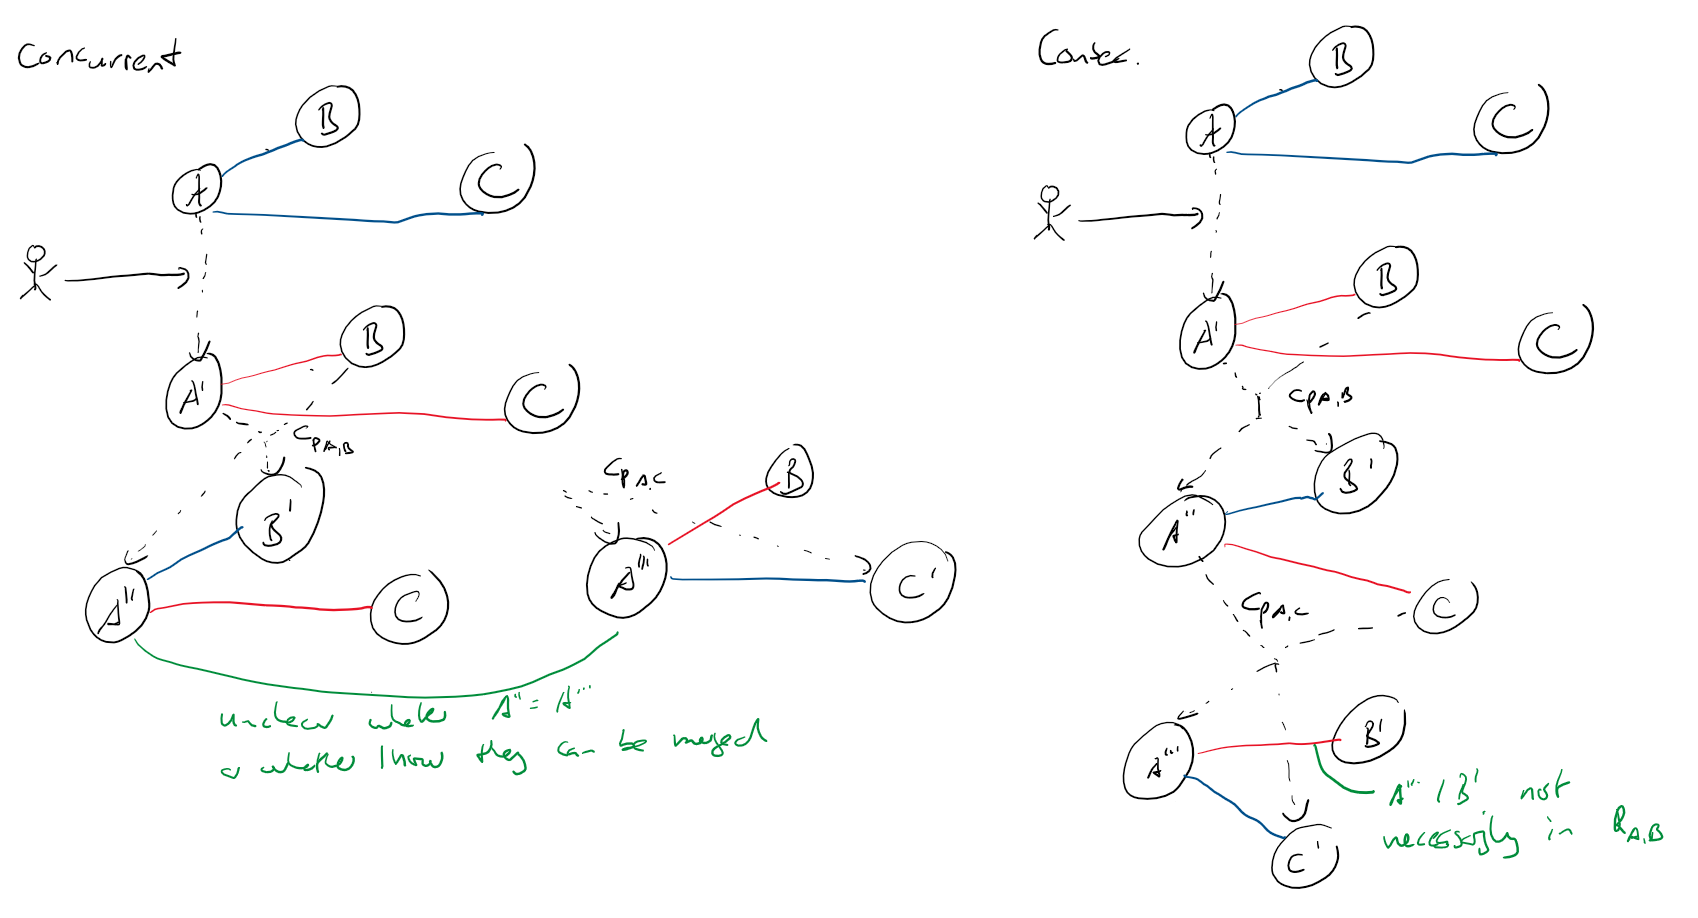
\includegraphics[width=\textwidth]{figures/correctness/formal/concurrent_consecutive_execution.png}
    \caption{Scenarios for independently executing consistency preservation rules on input models and consecutively executing them on the results of other rules.}
    \label{fig:correctness:concurrent_consecutive_execution}
\end{figure}

\mnote{Unification and orchestration necessary due to conflicting sequences}
The examples for the two strategies of executing \glspl{consistency preservation rule} are depicted in \autoref{fig:correctness:concurrent_consecutive_execution}. 
Even if \glspl{consistency preservation rule} were supposed to only modify one model instead of two, like in the examples, the same problems of unification and orchestration would occur as soon as there are two sequences of \glspl{consistency preservation rule} that change the same models.

\mnote{Benefits of consecutive execution}
In our work, we follow the approach of orchestrating and consecutively executing \glspl{consistency preservation rule}.
The benefits of this approach are twofold. First, there is no additional logic required for unifying the changes performed by independently executed \glspl{consistency preservation rule}. 
Second, the unification may deliver a model that is not consistent to any of the \glspl{consistency relation} anymore, whereas consecutive execution at least gives the guarantee that the models are consistent to the last applied \gls{consistency preservation rule}.
With this approach, the preservation rules can \enquote{negotiate} a solution by reacting to the changes the others performed.

\begin{remark} 
\mnote{Monolithic notions are degraded modular ones}
Finally, every monolithic notion of consistency and its preservation can be considered a special case of a modular notion. Having only one consistency relation and one function that preserves it degrades the problem by making the necessity to perform an orchestration of functions obsolete.
\end{remark}

\mnote{Different realization options for consistency preservation rules}
For now, the introduced \glspl{consistency preservation rule} can be any kind of functions that return consistent models. 
Their realization may, for example, be transformations that define how to react to certain changes for restoring consistency, or constraint solvers that find consistent models by solving consistency constraints. 
We do not yet need to consider how these functions are realized to derive consistent models, although, later, we will focus on transformation-based approaches.


\subsection{Declarative and Imperative Consistency Specifications}

\begin{figure}
    \centering
    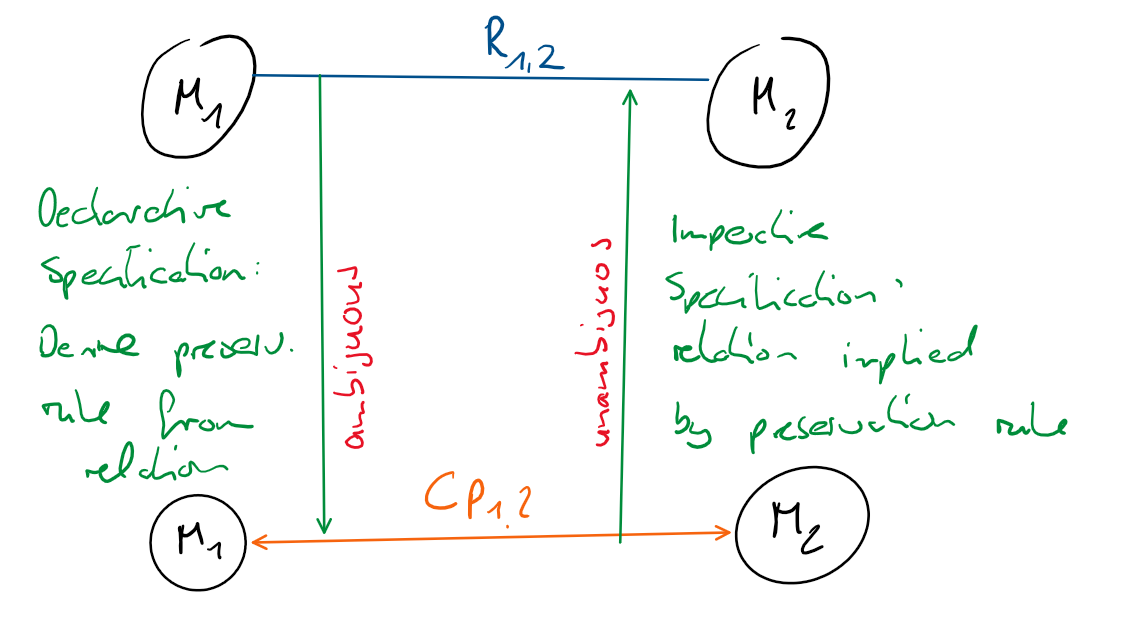
\includegraphics[width=0.7\textwidth]{figures/correctness/formal/declarative_imperative}
    \caption{Declarative and imperative specification of consistency relations and consistency preservation rules}
    \label{fig:correctness:declarative_imperative}
\end{figure}

\mnote{Only define relation \emph{or} function}
We discussed that consistency preservation can be considered as functions, called \glspl{consistency preservation rule}, that preserve consistency according to some relations.
%In practice, consistency preservation is usually specified by means of transformations.
In practice, however, one will usually not specify both the \gls{consistency relation} itself and also the \gls{consistency preservation rule} that preserves it.
Instead, usually one artifact is given and the other is implied or derived.
This leads to the two approaches of \emph{declarative} and \emph{imperative} consistency specifications, depending on whether the specification defines \emph{how} consistency is achieved.
The relation between the two approaches and \glspl{consistency relation} and \glspl{consistency preservation rule} is depicted in \autoref{fig:correctness:declarative_imperative}.

\mnote{Ambiguity in deriving rules from relations}
As a first option, a developer may only define relations that specifies consistency. Functions that preserve these relations can be derived from that.
This is called a \emph{declarative} specification, because it only declares when models are consistent but \emph{how} consistency is achieved.
In general, there is not only a single option how this function can look like.
It can, for example, calculate the result with minimal differences to the input, according to some defined metrics.
Or, especially if there is an intensional specification of that relation, the approach may consider the type of input change and calculate an appropriate change according to the constraints in the intensional specification.
This is the approach that is followed by many declarative transformation languages, such as \gls{QVTR}, or \glspl{TGG}.

\mnote{Relations are induced by fixed-points of functions}
As a second option, a developer can define \glspl{consistency preservation rule}.
These functions imply the underlying \glspl{consistency relation} that they preserve.
Given a function $\function{Cp}$, the relation is implied by its fixed-points: $\consistencyrelation{R}{} = \setted{\modelset{m} \mid \function{Cp}(\modelset{m}) = \modelset{m}}$.
If a function preserving consistency does not perform any changes, the models are, by definition, consistent.
This is called a \emph{imperative} specification, because it declares \emph{how} consistency can be achieved.
Such an approach is followed by many imperative transformation languages, such as \gls{QVTO} or \gls{VIATRA}.


\subsection{Artifacts in Consistency Preservation}

\mnote{Four artifacts for general consistency preservation}
We have discussed that consistency can be considered in a monolithic or modular way. We have, however, also mentioned that the monolithic case can be considered as a special case of the modular one.
For the general case, we thus know from the previous considerations that in a consistency preservation process at least specification that define consistency, called \emph{\glspl{consistency relation}}, functions that preserve consistency, called \emph{\glspl{consistency preservation rule}}, and a function for orchestrating the functions, in the following called \emph{\gls{orchestration function}}, are necessary. Finally, we also need a function that applies the \glspl{consistency preservation rule} in the order that is determined by the orchestration function, which we call the \emph{\gls{application function}}.
To summarize, we consider the following artifacts necessary to handle consistency preservation:
\begin{properdescription}
    \item[\Glspl{consistency relation}:] Binary (or in general n-ary) relations that specify when models are to be considered consistent.
    \item[\Glspl{consistency preservation rule}:] Functions that that restore consistency for a pair (or in general set) of models after they were modified to an inconsistent state.
    \item[\Gls{orchestration function}:] A function that determined in which order the consistency preservation rules have to be executed when the models became inconsistent.
    \item[\Gls{application function}:] A function that is able to apply the consistency preservation rules in the order determined by the orchestration function. 
\end{properdescription}

\mnote{Distinction between orchestration and application}
We explicitly distinguish the orchestration and the application to be able to make more fine-grained statements about the responsibilities for the orchestration and its actual execution.
The process is depicted in \autoref{fig:formal:executionprocess}. Given models that are consistent according to some consistency relations and changes to them that lead to inconsistencies, the orchestration function delivers an order of consistency preservation rules, which is used to parametrize the application function that executes these rules in the given order.
The result is, in the best case, a set of models that is consistent to the relations again.
However, we will see that this is not always possible. Thus, we will especially discuss relevant properties of the artifacts, such as correctness and optimality that reflect how and when this process can be executed successfully.

\begin{figure}
    \centering
    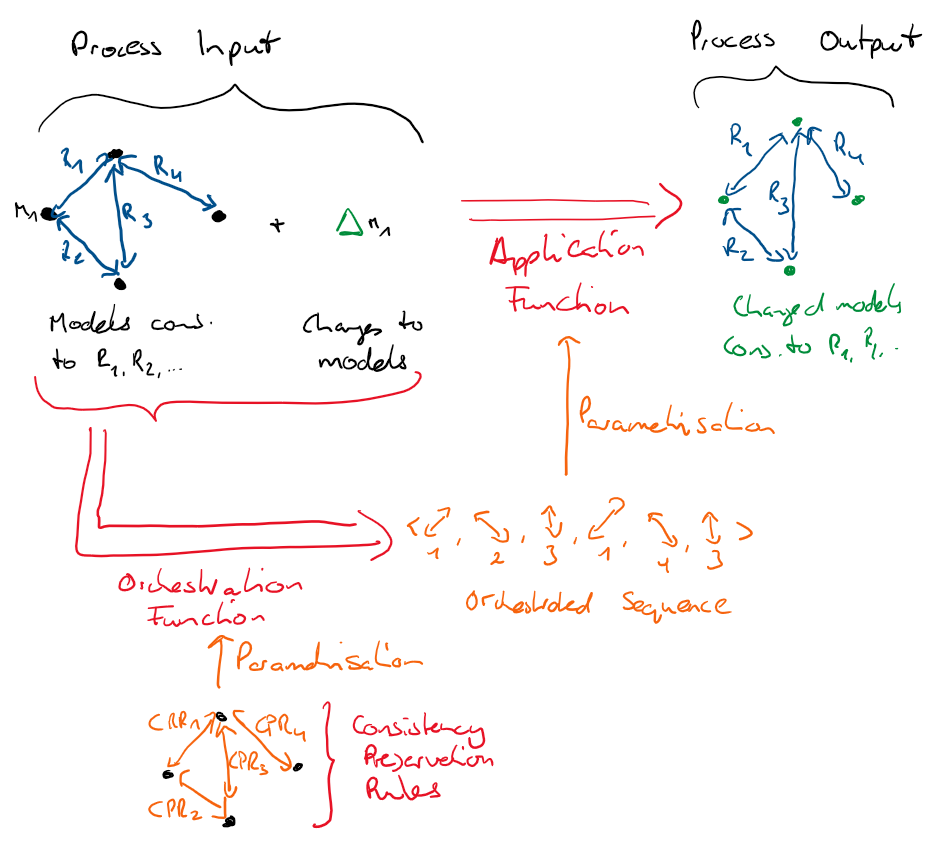
\includegraphics[width=\textwidth]{figures/correctness/formal/execution_process.png}
    \caption{Execution process and artifacts for a modular consistency specification}
    \label{fig:formal:executionprocess}
\end{figure}



%%
%% CORRECTNESS NOTIONS
%%
\section{Notions of Correctness for Consistency Specifications}

%\todo{Define correctness based on a networks adhering to the behavior of a multidirectional transformation}

%\todo{Korrektheit bx Netzwerk: es gib mx, deren Verhalten die bx emulieren müssen. Ist sehr stark, daher abschwächen. Ds muss nur kons. Zustand erreicht werden, egal wie? Einschränkung das original delta nicht geändert wird ist auch für mx künstlich.}

%\todo{Modular implies monolithic -> implicit correctness definition by implied relations}

\mnote{Different notions of correctness}
Before we formally define the above introduced artifacts, such as \glspl{consistency relation}, \glspl{consistency preservation rule}, an \gls{orchestration function} and an \gls{application function}, we first discuss different notions of \emph{correctness} for them.
Since there are different dimensions of correctness, we need to clarify which of them is relevant for us and will be defined in the formalization.

% \begin{definition}[Monolithic \ModelLevelConsistencyPreservationRule]
%     Given two metamodels $\metamodeltuple{M} = \tupled{\metamodelsequence{M}{n}}$ and a \modellevelconsistencyrelation between them $\consistencyrelation{CR}{} \subseteq \metamodelinstanceset{M}{1} \times \dots \times \metamodelinstanceset{M}{n}$.
%     A \emph{monolithic \modellevelconsistencypreservationrule} is a function:
%     \begin{align*}
%         \consistencypreservationrule{\consistencyrelation{CR}{}} : (\metamodeltupleinstanceset{M}, \metamodelinstanceset{M}{2}, \change{\metamodel{M}{1}}) \rightarrow \change{\metamodel{M}{2}}
%     \end{align*}
%     It that takes two consistent models and a change in the first one and returns a change in the second one.
%     We call a \modellevelconsistencypreservationrule \emph{correct} w.r.t. $\consistencyrelation{CR}{}$ if the resulting models when applying the input and output change are consistent to $\consistencyrelation{CR}{}$ again:
%     \begin{align*}
%         &
%         \forall \model{m}{1} \in \metamodelinstanceset{M}{1}, \model{m}{2} \in \metamodelinstanceset{M}{2} :
%         \tupled{\model{m}{1}, \model{m}{2}} \in \consistencyrelation{CR}{} \Rightarrow\\
%         & \formulaskip
%         \forall \change{\metamodel{M}{1}} \in \changeuniverse{\metamodel{M}{1}} :
%         \exists \change{\metamodel{M}{2}} \in \changeuniverse{\metamodel{M}{2}} :\\
%         & \formulaskip
%         \consistencypreservationrule{\consistencyrelation{CR}{}}(\model{m}{1}, \model{m}{2}, \change{\metamodel{M}{1}}) = \change{\metamodel{M}{2}} 
%         \land \tupled{\change{\metamodel{M}{1}}(\model{m}{1}), \change{\metamodel{M}{2}}(\model{m}{2})} \in \consistencyrelation{CR}{}
%     \end{align*}
% \end{definition}


\subsection{Relative Correctness Notions}

\mnote{Intuitive notion of correctness}
The overall objective regarding correctness of consistency preservation is to find models that are actually consistent.
Intuitively speaking, artifacts are correct if they fulfill their intended purpose. 
In our case this means, that consistency relations should consider models consistent whenever they are actually supposed to be considered consistent. 
\Glspl{consistency preservation rule} should return models that are actually consistent according to a \gls{consistency relation} to be considered correct.
This also conforms to the notion of correctness for transformations, which represent \glspl{consistency preservation rule}, defined by \textcite{stevens2010sosym}.
And finally, the orchestration and application functions should execute the \glspl{consistency preservation rule} such that all models are consistent according to all relations afterwards.

\mnote{Correctness is relative}
Correctness of an artifact is always considered with respect to some other specification, be it formally defined or only an informal notion.
For example, consistency relations may be supposed to be correct with respect to some informal notion of correctness that is collected by domain experts and requirements engineers.
A \gls{consistency preservation rule} should always be consistent with respect to a consistency relation. As discussed before, this relation may either be defined explicitly and the preservation rule has to be correct with respect to it, or it may be induced by the fixed points of the preservation rule.
In the latter case, the \gls{consistency preservation rule} will always be correct by construction.


\subsection{Correctness regarding Global Knowledge}

\mnote{Correctness of modular w.r.t. monolithic specification}
We previously distinguished between monolithic and modular notions of consistency.
In the above considerations, we relate the artifacts of a modular (or in the special case also a monolithic) specification to each other.
Another notion of correct, however, can also be defined by relating a modular artifact to a corresponding monolithic artifact.
For example, a set of modular \glspl{consistency relation} may be considered correct with respect to a monolithic relation when it considers the same sets of models consistent.
For three metamodels $\metamodel{M}{1}, \metamodel{M}{2}, \metamodel{M}{3}$ with three modular consistency relations $\consistencyrelation{R}{1,2}, \consistencyrelation{R}{1,3}, \consistencyrelation{R}{2,3}$ between them, as well as a ternary consistency relation $\consistencyrelation{R}{1,2,3}$, we could say that $\consistencyrelation{R}{1,2}, \consistencyrelation{R}{1,3}, \consistencyrelation{R}{2,3}$ are correct (with respect to $\consistencyrelation{R}{1,2,3}$) if and only if:
\begin{align*}
    & \forall \model{m}{1} \in \metamodel{M}{1}, \model{m}{2} \in \metamodel{M}{2}, \model{m}{3} \in \metamodel{M}{3}: \tupled{\model{m}{1}, \model{m}{2}, \model{m}{3}} \in \consistencyrelation{R}{1,2,3} \\
    & \formulaskip
    \equivalent \tupled{\model{m}{1}, \model{m}{2}} \in \consistencyrelation{R}{1,2} \land \tupled{\model{m}{1}, \model{m}{3}} \in \consistencyrelation{R}{1,3} \land \tupled{\model{m}{2}, \model{m}{3}} \in \consistencyrelation{R}{2,3}
\end{align*}
%
We may, analogously, define correctness for \glspl{consistency preservation rule}, an \gls{orchestration function}, and an \gls{application function} with respect to a single monolithic \gls{consistency preservation rule} by defining that both deliver the same results for the same inputs or at least return a consistent result in the same cases.

\begin{figure}
    \centering
    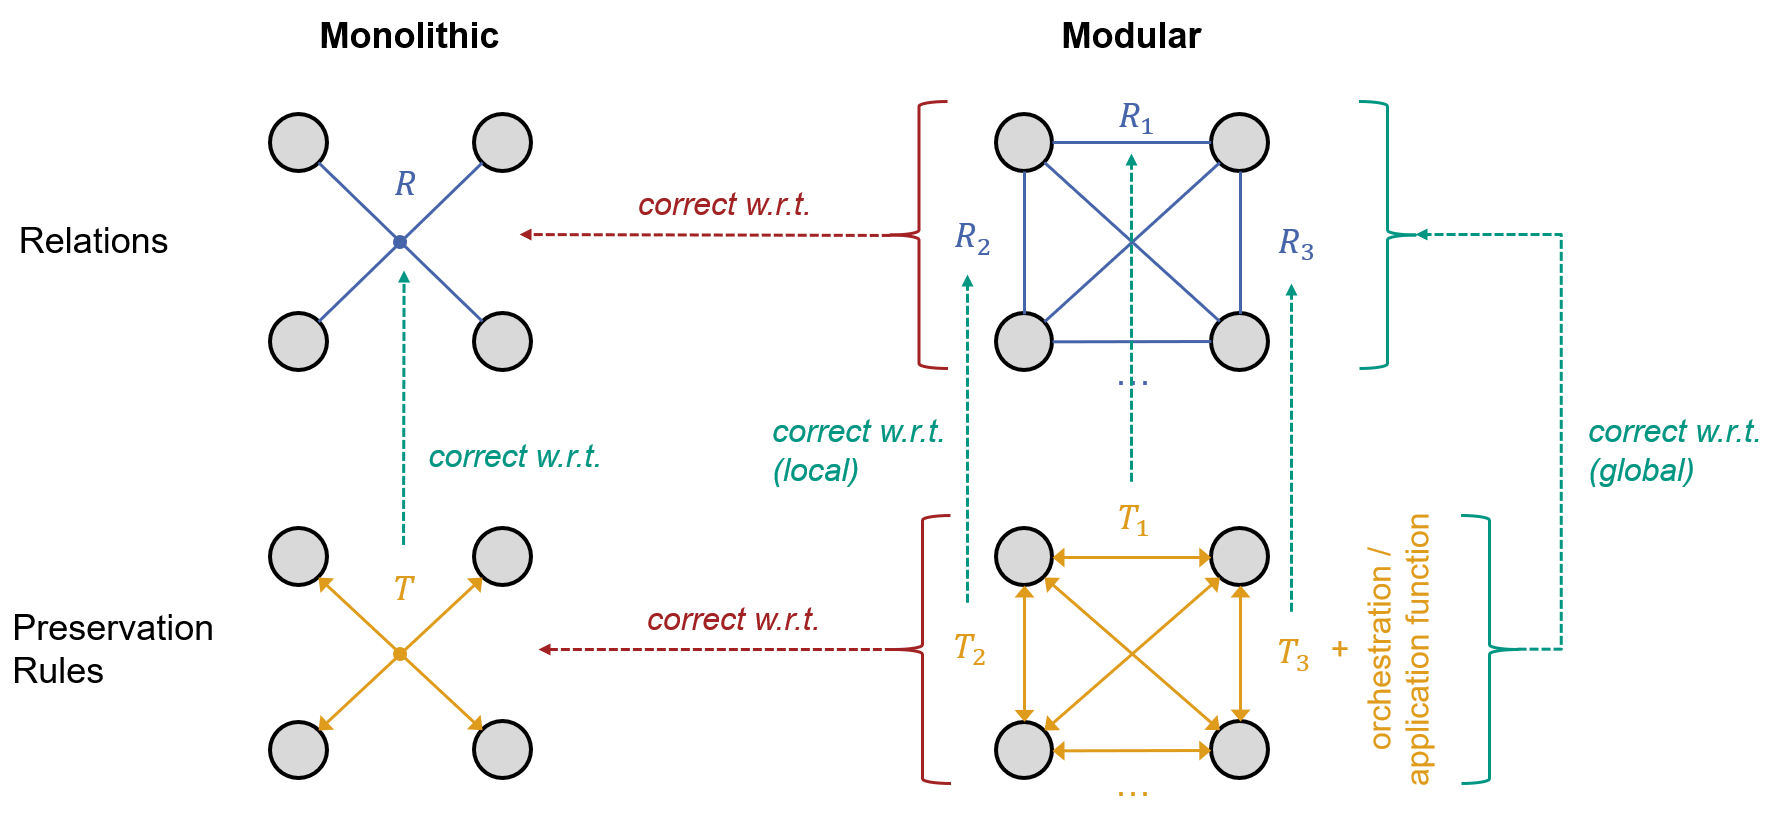
\includegraphics[width=\textwidth]{figures/correctness/formal/correctness_notions.png}
    \caption{Different notions of correctness for consistency and its preservation}
    \label{fig:correctness:correctnessnotions}
\end{figure}


\subsection{Dimensions of Correctness}

\mnote{Two dimension of correctness notions}
The discussed correctness notions introduce two dimension: First, correctness can be considered between artifacts within a monolithic or modular specification. Second, correctness can be considered between artifacts of a modular specification and corresponding artifacts of a monolithic specification. These dimension and correctness relations are depicted in \autoref{fig:correctness:correctnessnotions}.
The former dimension is depicted vertically. \Glspl{consistency preservation rule} need to be correct with respect to their \glspl{consistency relation}.
In the modular case, in addition to each preservation rule being \emph{locally} correct with respect to its relation, the combination of preservation rules by means of an orchestration and application function must also be correct with respect to the combination of all relations.
The latter dimension is depicted horizontally. Each modular artifact is supposed to be consistent with respect to its corresponding monolithic artifact.

\mnote{Drawbacks of global specification notions}
Although correctness of modular with respect to monolithic artifacts can be interesting from a theoretical perspective, its practical relevance is limited.
That notion of correctness assumes that there is some kind of global truth that has to be reflected by a modular specification.
This, however, has two essential drawbacks:
\begin{description}
    \item[Validation Artifacts:] The artifacts to check correctness against, i.e., the global, monolithic \gls{consistency relation} as well as an appropriate monolithic \gls{consistency preservation rule}, do usually not exist. If they existed, they could directly be used to preserve consistency. Thus, it is impossible to validate a set of \glspl{consistency relation} and \glspl{consistency preservation rule} against such a global specification.
    \item[Modular Knowledge:] This notion of correctness requires that the developers have some global knowledge that represents a monolithic \gls{consistency relation} and its \gls{consistency preservation rule}. As discussed before, we assume  the knowledge about relations between models to usually be distributed across several persons. Thus, there will no be such global knowledge, thus not even an implicit notion of the necessary artifacts to validate the modular specifications against. not to be mention an explicit representation.
\end{description}
%
Since this conflicts with our assumption of distributed knowledge about relations and independently developed, modular specification, we do not further consider this notion of consistency.
In this thesis, we focus on correctness between the artifacts of a modular consistency specification.


\subsection{Correctness of Consistency Relations}

\mnote{Correctness of relations}
The consistency notion that we consider in the following especially requires that \glspl{consistency preservation rule} and the functions to orchestrate and apply them must be correct with respect to \glspl{consistency relation}.
This notion, however, does not define when \glspl{consistency relation} are considered \emph{correct}.
One option is to only consider correctness with respect to monolithic artifacts for the case of \glspl{consistency relation}, as we proposed in previous work~\cite{klare2019icmt}.
This, however, suffers from the drawbacks discussed before, requiring a global notion of consistency.
Another notion of correctness would be conformance of the specified relations with what developers expect to be consistent, i.e., a validation of requirements.
For example, a consistency relation between UML and Java may only be considered correct if it fulfills some \enquote{natural} notion of consistency, as people know how elements have to be related because they represent similar things, such as classes, or because a standard like the UML~\cite{uml} prescribes that.
In this work, however, we do not consider such a correctness notion with respect to external, maybe not formally specified artifacts, which is part of separate research on requirements engineering and validation.

\mnote{Relations are not correct by construction}
In consequence, we might say that \glspl{consistency relation} are simply \emph{correct by construction}.
Thus, relations would normatively define what is to be considered consistent.
However, a consequence of not assuming a global knowledge of consistency is that different domain experts may have different notions of when models are to be considered consistent.
Consider for three metamodel $\metamodel{M}{1}, \metamodel{M}{2}, \metamodel{M}{3}$ the three modular \glspl{consistency relation} $\consistencyrelation{R}{1,2} = \setted{\tupled{\model{m}{1},\model{m}{2}}}, \consistencyrelation{R}{1,3} = \setted{\tupled{\model{m}{1},\model{m}{3}}}, \consistencyrelation{R}{2,3} = \setted{\tupled{\model{m}{1},\model{m'}{3}}}$. 
Then there is no triple of models that is considered consistent to all relations. 
Although we still do not want to assume a global knowledge about consistency to which the modular one must conform, we might say that these relations are \emph{incompatible}, as we do not want to combine relations that induce an empty set of consistent model tuples.
Identifying an appropriate notion of \emph{compatibility} and how to check it constitutes \researchquestionref{rq:correctness:compatibility} and will be discussed as our contribution \contributionref{contrib:correctness:compatility} in \autoref{chap:compatibility}.

\mnote{Modular relations induce monolithic ones}
In fact, every set of modular \glspl{consistency relation} induces a monolithic one.
This monolithic relation $\consistencyrelation{R}{}$ for metamodels $\metamodelsequence{M}{n}$ and pairwise consistency relations $\consistencyrelation{R}{i,j}$ is defined by:
\begin{align*}
    \consistencyrelation{R}{} = \setted{\tupled{\model{m}{1}, \dots, \model{m}{n}} \mid \bigwedge\limits_{1 \le i < j \le n} \tupled{\model{m}{i}, \model{m}{j}} \in \consistencyrelation{R}{i,j}}
\end{align*}
At least if this induced relation if empty, we probably want to consider the modular relations incompatible, because if no models are considered consistent, we cannot describe any system consistently.


% Keeping multiple models consistent by means of transformations imposes either a single multidirectional transformation or a combination of several bi- or multidirectional transformations.
% Each of these transformations is able to take a consistent tuple of models and a change to them and to return a new consistent tuple of models.

% \mnote{Correctness implicitly covered by definitions}
% \textcite{stevens2010sosym} proposes an explicit notion of \emph{correctness} for transformations. This is based on the fact that her definition of a transformation does only specify that for two given model, which may be inconsistent because one was modified, an update of the other model is returned.
% The requirement that the originally modified model and the one returned by the transformation have to conform to some consistency relations is specified externally as a notion of \emph{correctness}.
% We directly relate a consistency preservation rule that restores consistency to an according consistency relation, thus a consistency preservation rule that follows our definition is correct by construction in terms of the correctness definition by \citeauthor{stevens2010sosym}.
% The same applies to the consistency preservation application function, which we consider \emph{correct} if it fulfills its definition, as that definition already covers all requirements to that function.

% \mnote{Different notions of correctness}
% In general, correctness can be considered in two ways: First, an artifact may be correct if it simply follows its definition.
% While for consistency relations, changes and the generic \modellevelconsistencypreservationrule generalization function correctness can be canonically achieved, this is not that simple for a consistency preservation rule and the consistency preservation application function, as they have to fulfill some constraints with respect to consistency relations they rely on.
% Second, an artifact may be correct if it fulfills some, maybe only implicitly known specification. For example, a consistency relation between UML and Java may only be considered correct if it fulfills some \enquote{natural} notion of consistency, as people know how elements have to be related because they represent similar things, such as classes, or because a standard like the UML~\cite{uml} prescribes that.

% \mnote{Correctness regarding global specifications}
% In this work we do not consider the latter correctness notion with respect to external, maybe not formally specified artifacts, which is part of separate research on validation.
% However, when considering consistency of multiple models it may be standing to reason that a modular specification of consistency and its preservation has to be correct with regards to some global, monolithic specification. More precisely, there may be a multiary relation putting several metamodels into relation, which the developers at least implicitly know, and a set of binary relations somehow has to respect that multiary relation, i.e., be \emph{correct} with respect to that relation.
% The same can be imagines for consistency preservation. One may define a multidirectional transformation for a multiary relation, taking a tuple of changes to consistent models and retuning a new tuple of changes, which applied to the models delivers a consistent set of models again. In fact, this would be a realization of the behavior of the consistency preservation application function without relying on modular \modellevelconsistencypreservationrules.

% \begin{description}
%     \item[Validation Artifacts:] The artifacts to check correctness against, i.e., the global, multiary consistency relation as well as an appropriate multidirectional transformation, do usually not exist. If they existed, they could directly be used to preserve consistency. Thus is impossible to validate a set of consistency relations and preservation rules against such a global specification.
%     \item[Modular Knowledge:] This notion of correctness requires that the developers have some global knowledge that represents a monolithic, multiary consistency relation and their preservation rules. Usually, this will not be the case, so there is even no implicit notion of the necessary artifacts to validate the modular specifications against, not to be mention an explicit representation.
% \end{description}

%\todo{Add an image for that relation}

% Overall Goals:
% \begin{itemize}
%     \item Define correctness of a transformation network: termination in consistent state
% \end{itemize}



%%
%% FORMALIZATION
%%
\section{A Formal Notion of Transformation Networks}

\mnote{Goal: formalize transformation networks and correctness notions}
We yet discussed a general notion of consistency and its preservation with a focus on a modular way of specifying it.
This notion, however, was only specified in a rather informal way to first be able to discuss correctness notions and determine which notion is relevant for the considerations in this thesis.
In the following, we define a formal notion of consistency and its preservation, based on the informal explanation given before.
We also give a precise definition of notions for correctness between the artifacts of a modular specification.
Furthermore, we now focus on transformation-based approaches for preserving consistency, i.e., we consider specifications that transform changes within one or more models into changes in one or more other models.

Allgemeine Definition Transformationsnetzwerke:
\begin{itemize}
    %\item Definition Transformation aus Relation und Wiederherstellungsroutinen; Routinen nehmen n Modelle und n Deltasequenzen (eine pro Modell) und liefern n Deltasequenzen zurück.
    %\item Im Allgemeinen könnte eine Transformation beliebige dieser Deltasequenzen modifizieren. Wir verlangen jedoch, dass eine Transformation nur Deltas anhängt, also die Sequenzen länger werden
    %\item Genauer beschränken wir auch, welche Sequenzen eine Transformation sehen und ändern darf, genau gesagt darf sie die Sequenzen von zwei Modellen sehen und eine davon verlängern.
    %\item Hier kommt bereits der Unterschied zu bisherigen Transformationen, denn die sehen nur Deltas an einem Modell und erzeugen Deltas an dem anderen. Das ist bei uns schon gänzlich anders. Bidirektionale Transformationen unterstützen das im Übrigen auch nicht, sondern sind nur Spezifikationen, aus denen sich Wiederherstellungsroutinen für beide Richtungen ableiten lassen (siehe Stevens 2010)
    %\item Relationen in erster Instanz auf Modellebene (also bzgl. ganzer Modelle, nicht einzelner Modellelemente) definieren
    %\item Direkt als multidirektionale Transformation definieren, also beliebig viele geändert Ein- und Ausgabemodelle (oder jeweils nur eins?)
    %\item Korrektheit einer Transformation (nach Stevens) definieren!
    %item Versuchen den Konkatenationsoperator zu definieren ohne dass er alle Metamodelle referenzieren muss (also Transformation wählt aus einer großen Eingabemenge relevanten Modelle aus, ändert relevante und dann fügt der Operator sie in die große Menge ein)
    \item Definition Transformationsnetzwerk als Tupel aus Metamodellen, Transformationen und einer Ausführungsfunktion. 
    %\item Die Ausführungsfunktion führt für eine gegebene Änderung eine Auswahl der Transformationen nacheinander aus.
    \item Korrektheit eines Netzwerkes definieren: Die Ausführungsfunktion erzeugt eine Transformationssequenz, die angewendet auf eine Änderung für alle Änderungen ein korrektes Ergebnisse produziert, d.h. die Modelle sind konsistent bzgl. allen Konsistenzrelationen.
\end{itemize}


\subsection{Modular Consistency Specification}

\mnote{Extensional specifications are relations}
As already discussed informally before, an extensional specification of consistency enumerates all sets of models that are considered consistent to each other, i.e., it specifies a relation between the models.
Since it eases comprehension of the definitions if the considered models are identifiable with an index, we will consider, without loss of generality, tuples rather than sets of models throughout the rest of this thesis.

\begin{definition}[\ModelLevelConsistencyRelation]
    Given a tuple of metamodels $\metamodeltuple{M} = \tupled{\metamodelsequence{M}{n}}$, a \emph{\modellevelconsistencyrelation} $\consistencyrelation{CR}{}$ is a relation for instances of the metamodels $\consistencyrelation{CR}{} \subseteq \metamodeltupleinstanceset{M} = \metamodelinstanceset{M}{1} \times \dots \times \metamodelinstanceset{M}{n}$.

    For a tuple of models $\modeltuple{m} = \tupled{\model{m}{1}, \dots, \model{m}{n}} \in \metamodeltupleinstanceset{M}$ we say that:
    \begin{align*}
        \modeltuple{m} \consistenttomath \consistencyrelation{CR}{} \equivalentperdefinition \modeltuple{m} \in \consistencyrelation{CR}{}
    \end{align*}
    Otherwise, we call $\modeltuple{m} \mathtext{inconsistent to} \consistencyrelation{CR}{}$.
\end{definition}

\mnote{Start with coarse-grained model-level relations}
Given a tuple of models, we consider that tuple of models consistent if it is contained in the consistency relation.
This conforms to consistency definitions such as the one proposed by \textcite{stevens2010sosym} for bidirectional transformations.
We explicitly denote this kind of consistency relation as \emph{model-level}, because we will later need a more fine-grained notion of consistency relations at the level of \metaclasses and need to distinguish between the two.

\mnote{Modular notions of consistency}
If a single relation describes consistency between all relevant models, consistency is directly defined by means of model tuples being in that relations. We call such a relation a \emph{monolithic relation}.
However, if we have a \emph{modular} notion of consistency, i.e., a relation does only define consistency between some of the relevant models and the global notion of consistency is defined by a combination of several such relations, we need an explicit definition for that notion.
For the sake of simplicity, we focus on binary relations as a modular representation of consistency, but this definition could also be generalized to relations of arbitrary arity.
We assume that there is only one consistency relation between each pair of metamodels.
This assumption is without loss of generality, because two relations between the same metamodels are equivalent to only considering their intersection, i.e., only the model pairs that are considered consistent by both relations.

\todo{wlog: no direction of relation}

\begin{definition}[Consistency]
    Let $\metamodeltuple{M} =  \tupled{\metamodelsequence{M}{n}}$ be metamodels and let $\consistencyrelation{CR}{i,j} \subseteq \metamodelinstanceset{M}{i} \times \metamodelinstanceset{M}{j}$ be a binary \modellevelconsistencyrelation for any two metamodels $\metamodel{M}{i}, \metamodel{M}{j} \in \setted{\metamodelsequence{M}{n}}$.
    For a given tuple of models $\modeltuple{m} = \tupled{\model{m}{1}, \dots, \model{m}{n}} \in \metamodeltupleinstanceset{M}{} = \metamodelinstanceset{M}{1} \times \dots \times \metamodelinstanceset{M}{n}$, we say that this model tuple is \emph{consistent to} $\consistencyrelation{CR}{i,j}$ if and only if the instances of $\metamodel{M}{i}$ and $\metamodel{M}{j}$ are in that relation:
    \begin{align*} 
        &
        \modeltuple{m} = \tupled{\model{m}{1}, \dots, \model{m}{n}} \consistenttomath \consistencyrelation{CR}{i,j} \equivalentperdefinition %\\
        %& \formulaskip
        \tupled{\model{m}{i},\model{m}{j}} \in \consistencyrelation{CR}{i,j}
        %\exists \model{m}{i} \in \metamodelinstanceset{M}{i}, \model{m}{j} \in \metamodelinstanceset{M}{j} : \model{m}{i} \in \modelset{m} \land \model{m}{j} \in \modelset{m} \land \tupled{\model{m}{i}, \model{m}{j}} \in \consistencyrelation{CR}{}
    \end{align*}
    For a set of binary \modellevelconsistencyrelations $\consistencyrelationset{CR}$ for metamodels $\metamodeltuple{M}$, we say that a tuple of models $\modeltuple{m} \in \metamodeltupleinstanceset{M}{}$ is \emph{consistent to} $\consistencyrelationset{CR}$ if and only if it is consistent to each consistency relation in that set:
    \begin{align*} 
        &
        \modeltuple{m} \consistenttomath \consistencyrelationset{CR} \equivalentperdefinition %\\
        %& \formulaskip
        \forall \consistencyrelation{CR}{} \in \consistencyrelationset{CR} : \modeltuple{m} \consistenttomath \consistencyrelationset{CR}
    \end{align*}
\end{definition}

\mnote{Examplary binary relations}
The definition states that given a set of \modellevelconsistencyrelations the models must be consistent to all of these relations to consider them consistent to the set.
Consider, for example, the relations $\consistencyrelation{CR}{1} = \setted{\tupled{\model{m}{1}, \model{m}{2}}}$, $\consistencyrelation{CR}{2} = \setted{\tupled{\model{m}{2},\model{m}{3}}}$, $\consistencyrelation{CR}{3} = \setted{\tupled{\model{m}{1}, \model{m}{3}}}$ with $\model{m}{i} \in \metamodelinstanceset{M}{i}$ for metamodels $\metamodel{M}{i}$. Then the model tuple $\tupled{\model{m}{1}, \model{m}{2}, \model{m}{3}}$ is consistent to these relations, because it is consistent to each of the binary relations.
These consistency relations are equivalent to a monolithic relation $\consistencyrelation{CR}{} = \setted{\tupled{\model{m}{1}, \model{m}{2}, \model{m}{3}}}$, because a model tuple $\modeltuple{m}$ is consistent to $\consistencyrelation{CR}{}$ exactly when it is consistent to $\setted{\consistencyrelation{CR}{1}, \consistencyrelation{CR}{2}, \consistencyrelation{CR}{3}}$.


\subsection{Expressiveness of Modular Consistency Specifications}

\mnote{Modular and monolithic specification are not equivalent}
Although in that exemplary case the binary relations are equivalent to a monolithic relation, such an equivalence is not always given. In general, two interesting insights come along with that definition of consistency based on modular relations. First, expressiveness of defining consistency modularly by a set of relations is not equivalent to defining one monolithic relation between all models. Second, a modular definition of consistency can easily contain contradictions, which may lead to an empty set of consistent models.

\mnote{Binary relations reduce expressiveness}
It is easy to see that a combination of binary relations is not able to express the same consistency relations as one monolithic relation.
For example, the monolithic relation $\consistencyrelation{CR}{} = \setted{\tupled{\model{m}{1}, \model{m}{2}, \model{m}{3}'}, \tupled{\model{m}{1}, \model{m}{2}', \model{m}{3}}, \tupled{\model{m}{1}', \model{m}{2}, \model{m}{3}}}$ cannot be expressed by binary relations.
The binary relations necessarily need to contain $\tupled{\model{m}{1}, \model{m}{2}}$, because $\tupled{\model{m}{1}, \model{m}{2}, \model{m}{3}'} \in \consistencyrelation{CR}{}$ and $\tupled{\model{m}{2}, \model{m}{3}}$, because $\tupled{\model{m}{1}', \model{m}{2}, \model{m}{3}} \in \consistencyrelation{CR}{}$. However, this would mean that $\tupled{\model{m}{1}, \model{m}{2}, \model{m}{3}}$ is considered consistent to the binary relations although it not consistent to the modular relation $\consistencyrelation{CR}{}$.
Thus, using sets of binary relations in contrast to a single monolithic relation reduces expressiveness.
\textcite{stevens2017a} discusses the property of a multiary relation to be expressed by binary ones as \emph{binary-definable} in detail.
She proposed restrictions to binary relations that may be sufficient and still practical for expressing consistency, such as a notion of \emph{binary-implemented} relations.
However, we reasoned the assumption that relations need to be specified independently and thus modularly anyway, thus we have to accept that these restrictions in expressiveness exists.
\todo{visualize}

\mnote{Binary relations may be contradictory}
Additionally, it is easy to define multiple binary relations of which each can be fulfilled by certain models, but for which no tuple of models exists that is consistent to all of them. Consider the relations $\consistencyrelation{CR}{1} = \setted{\tupled{\model{m}{1}, \model{m}{2}}}$, $\consistencyrelation{CR}{2} = \setted{\tupled{\model{m}{2}, \model{m}{3}}}$, $\consistencyrelation{CR}{3} = \setted{\tupled{\model{m}{1}, \model{m}{3}'}}$.
Although for each of these relations a consistent set of models exists, which is exactly the one defined in each relation, no tuple of models exists that fulfills their combination.
This example already demonstrates the worst case, in which no consistent models exist for a set of relations.
In other cases, it may be possible that only for some models that are consistent according to one or some of the relations no model tuple exists that is consistent for all models.
Consider the relations $\consistencyrelation{CR}{1} = \setted{\tupled{\model{m}{1}, \model{m}{2}}}$, $\consistencyrelation{CR}{2} = \setted{\tupled{\model{m}{2}, \model{m}{3}}, \tupled{\model{m}{2}, \model{m}{3}}'}$, $\consistencyrelation{CR}{3} = \setted{\model{m}{1}, \model{m}{3}'}$.
In this case, the tuple $\tupled{\model{m}{1}, \model{m}{2}, \model{m}{3}'}$ would be considered consistent to the relations, but although $\tupled{\model{m}{2}, \model{m}{3}} \in \consistencyrelation{CR}{2}$ there exists no $\model{m^*}{1} \in \metamodelinstanceset{M}{1}$ so that $\tupled{\model{m^*}{1}, \model{m}{2}, \model{m}{3}}$ is consistent to all these relations.
\todo{visualize}

\mnote{Sets of relations can forbid models}
It is easy to see that one monolithic relation may be equally represented by an arbitrary number of sets of binary relations by simply adding model pairs to these binary relations that are never consistent to the other relations, like we have seen for the pair $\tupled{\model{m}{2}, \model{m}{3}}$ in the previous example.
This means that the combination of relations can lead to the situation that some models are actually forbidden (like $\model{m}{3}$ in the example before) due to the combination of consistency relations.
We already informally discussed this as a notion of \emph{compatibility}, for which we investigate in \autoref{sec:correctness:compatibility} how far this behavior is or should be expected.


\subsection{Incremental and Inductive Consistency Preservation}

\mnote{Preserving consistency}
While the previous discussion only considered when models are considered consistent, it is of especial interest to ensure that consistency of models is preserved.
We informally introduced such specifications as \glspl{consistency preservation rule}.
In the following, we will restrict us to \emph{incremental} and \emph{inductive} consistency preservation and give a precise definition for that.
This means that we make the following assumptions to the process:
\begin{properdescription}
    \item[Information preservation (incrementality):] After a change to one model, the others are not generated from scratch but updated according to the performed changes. This ensures that information that cannot be generated but was added by users to the other models is preserved.
    \item[Consistency assumption (induction):] We assume models to be consistent before a change is processed by \glspl{consistency preservation rule}. Otherwise the preservation rules would need to be able to handle arbitrary states of the models and it would be unclear consistency to which \glspl{consistency relation} has to be restored.
\end{properdescription}
While incrementality is an essential requirement whenever consistency shall be preserved to avoid information loss, inductivity may not be necessary.
We, however, make this assumption to avoid requiring from the \glspl{consistency preservation rule} that they need to be able to process an inconsistent state without knowing which changes introduced it.
From a theoretical point of view, we could omit that requirement, but this would make the specification of \glspl{consistency preservation rule} impractically complicated, such that omitting that requirement is not practically relevant anyway.
%In consequence, an incremental and inductive \gls{consistency preservation rule} takes a consistent tuple of models and changes to them and returns a tuple of models that is consistent again.

\todoLater{Do we need inductivity for synchronization? Otherwise we may remove it here and from following definitions?}
%\todo{Explicitly discuss incrementality here, although we actually do not need it. So leave it out? No, needed for synchronization definition. But make clear that this is a specialization and discuss generalization.}
%\todo{Make precise here that we have incremental consistency, thus last consistent state and delta to that is known. We did not assume that in the informal notion before.}

\mnote{Monolithic and modular consistency preservation}
Like we already discussed for \glspl{consistency preservation rule} in general, incremental preservation rules can be realized in an either monolithic or modular way.
A monolithic consistency preservation rules takes a tuple of models that is consistent to a consistency relation and a change to these models and returns another tuple of models that is consistent again.
In a modular specification of \glspl{consistency preservation rule}, a set of such rules is given which are able to preserve consistency of a subset of the given models according to modular consistency relations.
In our case, we consider such rules for two models, each of them restoring consistency according to a binary consistency relation.
%We will later discuss if and how an execution order of such consistency preservation rules can be determined.

\mnote{Drawbacks of existing unidirectional consistency restorers}
In terminology for transformations, a \gls{consistency preservation rule} that restores consistency of models according to a \gls{consistency relation} in one direction is called \emph{directional transformation}~\cite{stevens2010sosym} or \emph{consistency restorer}~\cite{stevens2020BidirectionalTransformationLargeSoSym}.
Definitions of that terminology do usually not consider changes but only states of models and simply define a preservation rule for metamodel $\metamodel{M}{1}$ and $\metamodel{M}{2}$ that modifies the instance of $\metamodel{M}{2}$ to restore consistency as $\consistencypreservationrule{}: \metamodelinstanceset{M}{1} \times \metamodelinstanceset{M}{2} \rightarrow \metamodelinstanceset{M}{2}$.
This notion, however, has two properties that imply essential drawbacks:
\begin{properdescription}
    \item[State-based:] No information about the performed changes that led to the inconsistent state are given. This means that the specification is not aware of how the inconsistent state was reached.
    \item[Unidirectional:] The unidirectionality of the specification always requires to only update one model to restore consistency.
\end{properdescription}
State-based transformations always suffer from the problem that it is unknown which changes were made that led to an inconsistent state and reconstructing them from the difference between two states is only a heuristic approximation~\cite{diskin2011StateToDeltaSymmetric-MODEDLS}.
This, for example, includes that information about elements which were moved or renamed can potentially not be reconstructed, leading to elements that are deleted and created anew, losing all information that was potentially added to them.
Unidirectionality may be reasonable when assuming that only one of the models was modified. In that case it is sufficient to update the other model to restore consistency.
With a modular specification of consistency preservation, however, several \glspl{consistency preservation rule} modifying the same models may need to be executed.
This can be seen in the example in \autoref{todo}\todo{add graphics and explanation for that}.
In consequence, the rules need to be able to deal with changes performed in both of the input models and, consequentially, need to update both models to reflect the changes in the other.

\mnote{Synchronizing consistency preservation rules circument drawbacks}
To be able to combine several \glspl{consistency preservation rule} without the discussed drawbacks, we define a \emph{synchronizing} rather than a unidirectional notion of them
Those rules are able to react to changes in both models and produce changes in both models again.
To precisely define this behavior, we first introduce a notion of \emph{changes} and afterwards of \emph{\glspl{consistency preservation rule}}.

\begin{definition}[Change]
    Given a metamodel $\metamodel{M}{}$, a change $\change{\metamodel{M}{}}$ is a function that takes an instance of that metamodel and returns another one:
    \begin{align*}
        \change{\metamodel{M}{}}: \metamodelinstanceset{M}{} \rightarrow \metamodelinstanceset{M}{}
    \end{align*}
    It encodes any kind of modification, which may be just an element addition, or removal, an attribute change and so on, or any composition of changes.
    We denote the identity change, i.e., the change that always returns the input model, as $\identitychange$:
    \begin{align*}
        \identitychange(x) \equalsperdefinition x
    \end{align*}
    We denote the universe of all changes in $\metamodel{M}{}$, i.e., all subsets of $\metamodelinstanceset{M}{} \times \metamodelinstanceset{M}{}$ that are functional, as 
    \begin{align*}
        \changeuniverse{\metamodel{M}{}} \equalsperdefinition \setted{\change{\metamodel{M}{}} \mid \change{\metamodel{M}{}} \subseteq \metamodelinstanceset{M}{} \times \metamodelinstanceset{M}{} \land
        (\tupled{\model{m}{1}, \model{m}{2}}, \tupled{\model{m}{1}, \model{m}{3}} \in \change{\metamodel{M}{}} \Rightarrow \model{mc}{2} = \model{m}{3})}
    \end{align*}
    For a given metamodel tuple $\metamodeltuple{M} = \tupled{\metamodelsequence{M}{n}}$, we denote the set of all tuples of changes in the instances tuples of 
    $\metamodeltuple{M}$, i.e. in $\metamodeltupleinstanceset{M}$, as $\changeuniverse{\metamodeltuple{M}}$:
    \begin{align*}
        \changeuniverse{\metamodeltuple{M}} \equalsperdefinition \setted{ \changetuple{\metamodeltuple{M}} = \tupled{\change{\metamodel{M}{1}}, \dots, \change{\metamodel{M}{n}}} \mid \forall i \in \setted{1,\dots,n} : \change{\metamodel{M}{i}} \in \changeuniverse{\metamodel{M}{i}} } 
    \end{align*}
\end{definition}

\mnote{Behavior of unapplicable change is undefined}
For us, it does not matter how the function describing a change behaves in cases, in which the encoded change cannot be applied, e.g., because the changed or removed element does not exist. The function may do nothing for those models, i.e., return the identical model, or even be undefined for those model, i.e., be partial.
\todoLater{Check whether this behavior is correct.}

% \begin{definition}[\ModelLevelConsistencyPreservationRule]
%     Let $\metamodel{M}{1}, \metamodel{M}{2}$ be two metamodels and $\consistencyrelation{CR}{} \subseteq \metamodelinstanceset{M}{1} \times \metamodelinstanceset{M}{2}$ a binary \modellevelconsistencyrelation between them.
%     A \emph{\modellevelconsistencypreservationrule} $\consistencypreservationrule{\consistencyrelation{CR}{}}$ for the relation $\consistencypreservationrule{\consistencyrelation{CR}{}}$ is a function:
%     \begin{align*}
%         \consistencypreservationrule{\consistencyrelation{CR}{}} : (\metamodelinstanceset{M}{1}, \metamodelinstanceset{M}{2}, \change{\metamodel{M}{1}}) \rightarrow \change{\metamodel{M}{2}}
%     \end{align*}
%     It takes two consistent models and a change in the first one and returns a change in the second one.
%     We call a \modellevelconsistencypreservationrule \emph{correct} w.r.t. $\consistencyrelation{CR}{}$ if the resulting models when applying the input and output change are consistent to $\consistencyrelation{CR}{}$ again:
%     \begin{align*}
%         &
%         \forall \model{m}{1} \in \metamodelinstanceset{M}{1}, \model{m}{2} \in \metamodelinstanceset{M}{2} :
%         \tupled{\model{m}{1}, \model{m}{2}} \in \consistencyrelation{CR}{} \Rightarrow\\
%         & \formulaskip
%         \forall \change{\metamodel{M}{1}} \in \changeuniverse{\metamodel{M}{1}} :
%         \exists \change{\metamodel{M}{2}} \in \changeuniverse{\metamodel{M}{2}} :\\
%         & \formulaskip
%         \consistencypreservationrule{\consistencyrelation{CR}{}}(\model{m}{1}, \model{m}{2}, \change{\metamodel{M}{1}}) = \change{\metamodel{M}{2}} 
%         \land \tupled{\change{\metamodel{M}{1}}(\model{m}{1}), \change{\metamodel{M}{2}}(\model{m}{2})} \in \consistencyrelation{CR}{}
%     \end{align*}
% \end{definition}

\begin{definition}[\ModelLevelConsistencyPreservationRule]
    \label{def:consistencypreservationrule}
    Let $\metamodel{M}{1}, \metamodel{M}{2}$ be two metamodels and $\consistencyrelation{CR}{} \subseteq \metamodelinstanceset{M}{1} \times \metamodelinstanceset{M}{2}$ a binary \modellevelconsistencyrelation between them.
    A \emph{\modellevelconsistencypreservationrule} $\consistencypreservationrule{\consistencyrelation{CR}{}}$ for the relation $\consistencypreservationrule{\consistencyrelation{CR}{}}$ is a function:
    \begin{align*}
        \consistencypreservationrule{\consistencyrelation{CR}{}} : (\metamodelinstanceset{M}{1}, \metamodelinstanceset{M}{2}, \changeuniverse{\metamodel{M}{1}}, \changeuniverse{\metamodel{M}{2}}) \rightarrow (\changeuniverse{\metamodel{M}{1}}, \changeuniverse{\metamodel{M}{2}})
    \end{align*}
    %It takes two consistent models and a change in the first one and returns a change in the second one. 
\end{definition}

\mnote{Correctness notion of consistency preservation rules}
To consider a \modellevelconsistencypreservationrule \emph{correct}, it has to return changes that, when applied to the input models, result in models that are consistent according to the \modellevelconsistencyrelation for which the preservation rule is defined.
This conforms to the notion of correctness defined for bidirectional transformations~\cite{stevens2010sosym}.

\begin{definition}[\ModelLevelConsistencyPreservationRule Correctness]
    \label{def:consistencypreservationrulecorrectness}
    Let $\consistencypreservationrule{\consistencyrelation{CR}{}}$ be a \emph{\modellevelconsistencypreservationrule}.
    We call a \modellevelconsistencypreservationrule \emph{correct} if the resulting models when applying the generated changes are consistent to $\consistencyrelation{CR}{}$ again:
    \begin{align*}
        &
        \forall 
        \model{m}{1} \in \metamodelinstanceset{M}{1}, 
        \model{m}{2} \in \metamodelinstanceset{M}{2},
        \change{\metamodel{M}{1}} \in \changeuniverse{\metamodel{M}{1}},
        \change{\metamodel{M}{2}} \in \changeuniverse{\metamodel{M}{2}} :
        \tupled{\model{m}{1}, \model{m}{2}} \in \consistencyrelation{CR}{} \Rightarrow\\
        & \formulaskip
        \exists 
        \change{\metamodel{M}{1}}' \in \changeuniverse{\metamodel{M}{1}},
        \change{\metamodel{M}{2}}' \in \changeuniverse{\metamodel{M}{2}} :
        \consistencypreservationrule{\consistencyrelation{CR}{}}(\model{m}{1}, \model{m}{2}, \change{\metamodel{M}{1}}, \change{\metamodel{M}{2}}) = (\change{\metamodel{M}{1}}', \change{\metamodel{M}{2}}') \\
        & \formulaskip
        \land \tupled{\change{\metamodel{M}{1}}'(\model{m}{1}), \change{\metamodel{M}{2}}'(\model{m}{2})} \in \consistencyrelation{CR}{}
    \end{align*}
\end{definition}

\mnote{No restriction to achieve \enquote{resonable} preservation rules}
This definition does not make any restrictions on how the input and output changes are related.
In fact, a valid (and especially correct) \gls{consistency preservation rule} could always return empty changes.
In consequence, the rule would simply revert all input changes to achieve a consistent state again.
Although this may not be the expected behavior, there is no reason to restrict this behavior in the definition.
Actually, the developer of the preservation rule should specify in a \emph{reasonable} way, such that is provides any expected behavior.

%A \modellevelconsistencypreservationrule is defined to restore consistency after a modification in a left model of the underlying \modellevelconsistencyrelation by creating a change for the right model. To consider consistency preservation rules that preserve consistency in the other direction, we regard the inverse of the consistency relation as well, denoted as $\inverseconsistencyrelation{CR}{} = \setted{\tupled{\model{m}{1}, \model{m}{2}} \mid \tupled{\model{m}{2}, \model{m}{1}} \in \consistencyrelation{CR}{}}$.

\mnote{Encapsulation of consistency relations and preservation rules in transformations.}
We already discussed that it is possible to define \glspl{consistency relation} and derive \glspl{consistency preservation rule} from them or to only define the \glspl{consistency preservation rule}, which then imply the \glspl{consistency relation} by their fixed points.
Anyway, in practice there will only be one of these specifications and the other is implied or derived.
We thus define a \emph{synchronizing transformation}, in extension to \emph{bidirectional transformations}~\cite{stevens2010sosym}, as an artifact that encapsulates a \modellevelconsistencyrelation together with a \modellevelconsistencypreservationrule, no matter which of them is defined and which is derived or implied.

\begin{definition}[Synchronizing Transformation]
    \label{def:synchronizingtransformation}
    Let $\consistencyrelation{CR}{}$ be a \modellevelconsistencyrelation and $\consistencypreservationrule{\consistencyrelation{CR}{}}$ a \modellevelconsistencypreservationrule that restores consistency according to that relation.
    A \emph{synchronizing transformation} is a pair $\transformation{T} = \tupled{\consistencyrelation{CR}{}, \consistencypreservationrule{\consistencyrelation{CR}{}}}$.
\end{definition}

\begin{definition}[Synchronizing Transformation Correctness]
    \label{def:synchronizingtransformationcorrectness}
    We call a synchronizing transformation $\transformation{T} = \tupled{\consistencyrelation{CR}{}, \consistencypreservationrule{\consistencyrelation{CR}{}}}$ if, and only if, $\consistencypreservationrule{\consistencyrelation{CR}{}}$ is correct according to \autoref{def:consistencypreservationrulecorrectness}.
\end{definition}

In the following, we will only refer to transformations rather than \glspl{consistency preservation rule} if the distinction is not necessary.
Although \autoref{def:synchronizingtransformationcorrectness} precisely defines when we consider a transformation correct, it is unclear how to define a transformation that fulfills such a correctness property.
This question was introduced as \researchquestionref{rq:correctness:synchronization} and an approach for that constitues our contribution \contributionref{contrib:correctness:synchronization}, which we discuss in \autoref{chap:synchronization}.


\subsection{Transformation Orchestration}

\mnote{Multiple transformations need orchestration}
Having multiple transformations between several metamodels requires their orchestration, i.e., the decision which transformation have to be executed in which order, if consistency between instances of those metamodels shall be preserved after changes.
We discussed that transformations, or more precisely their \glspl{consistency preservation rule}, may be executed independently and thus concurrently, which requires their results to be unified, or to execute them consecutively.
We already identified the drawbacks of a concurrent execution approach, including the necessity to define unification operators and the missing guarantee to be consistent to any consistency relation after such a unification.
This is why we follow the approach of consecutively executing transformations.

\mnote{Orchestration function to determine execution order}
To consecutively execute transformations, an order of their execution has to be determined.
While in practice a dynamic algorithm will be used to determine that order, from a theoretical perspective that algorithm realized a function that returns the order to execute the transformations in.
We call this an \emph{orchestration function} as it is responsible for orchestrating the execution of transformations.

\begin{definition}[Transformation Orchestration Function]
    Let $\transformationset{}$ be a set of transformations with \glspl{consistency relation} and according \glspl{consistency preservation rule} for metamodels $\metamodeltuple{M} = \tupled{\metamodelsequence{M}{n}}$.
    A transformation \gls{orchestration function} $\orcfunction{\transformationset{T}}$ for these transformations is a function:
    \begin{align*}
        &
        \orcfunction{\transformationset{T}} : (\metamodeltupleinstanceset{M}, \changeuniverse{\metamodeltuple{M}}) \rightarrow \transformationset{T}^{< \mathbb{N}}
    \end{align*}
    $\transformationset{T}^{< \mathbb{N}}$ denotes all finite sequences of transformations in $\transformationset{T}$, i.e., $\transformationset{T}^{< \mathbb{N}} = \emptyset \cup \transformationset{T}^1 \cup \transformationset{T}^2 \cup \dots$.
\end{definition}

% \begin{definition}[Consistency Preservation Orchestration Function]
%     Let $\consistencypreservationruleset{}$ be a set of consistency preservation rules for a set of consistency relations $\consistencyrelationset{CR}$ on metamodels $\metamodeltuple{M} = \tupled{\metamodelsequence{M}{n}}$.
%     A consistency preservation orchestration function $\consistencyorcfunction{\consistencypreservationruleset{}}$ for these rules is a function:
%     \begin{align*}
%         &
%         \consistencyorcfunction{\consistencypreservationruleset{}} : (\metamodeltupleinstanceset{M}, \changeuniverse{\metamodeltuple{M}}) \rightarrow \consistencypreservationruleset{}^{< \mathbb{N}}
%     \end{align*}
%     $\consistencypreservationruleset{}^{< \mathbb{N}}$ denotes all finite sequences of consistency preservation rules in $\consistencypreservationruleset{}$, i.e., $\consistencypreservationruleset{}^{< \mathbb{N}} = \emptyset \cup \consistencypreservationruleset{}^1 \cup \consistencypreservationruleset{}^2 \cup \dots$.
% \end{definition}

\mnote{Orchestration function does not guarantee consistent result}
According to this definition, the orchestration functions returns a sequence of transformations and determines that their \modellevelconsistencypreservationrules need to be executed in the given order. 
This especially includes that transformations may occur more than once in such sequence.

\mnote{There is not always an orchestration with a consistent result}
It is obvious that without further restrictions to the transformations it is possible that for given transformations, models and changes to them an orchestration function cannot find an execution order that returns a consistent tuple of models after certain changes. 
Consider the example in \autoref{fig:formal:noexecutionorder}. There exists no execution order for any input value that terminates. The transformations will always increase the value, although the defined relations could be fulfilled for the input value, but the transformations never find that solution.

\begin{figure}
    \centering
    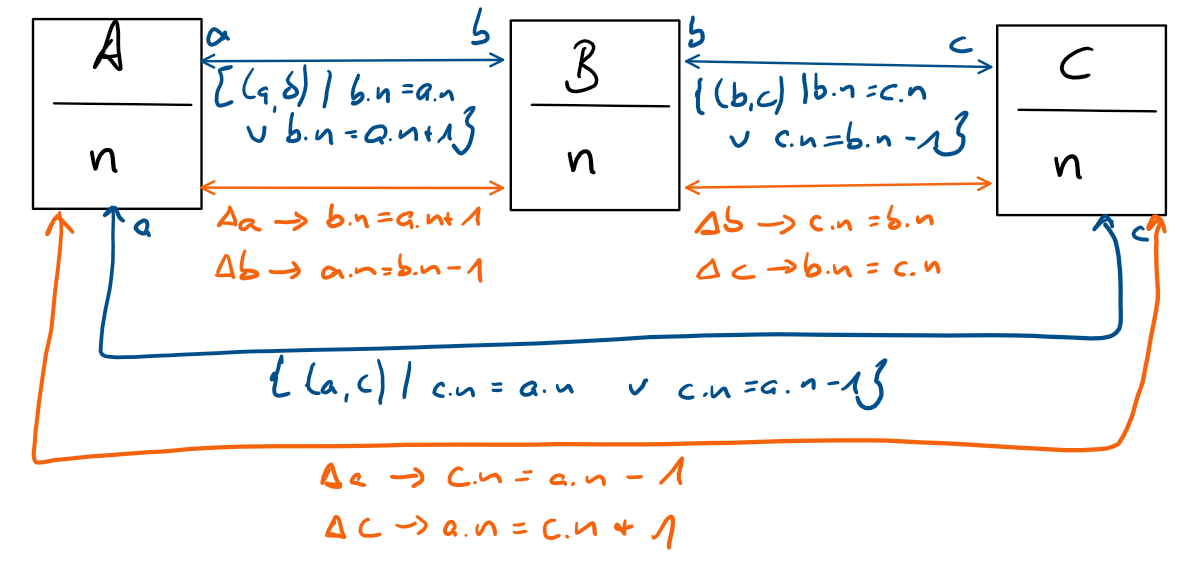
\includegraphics[width=\textwidth]{figures/correctness/formal/divergence_example.png}
    \caption{Example for divergence}
    \label{fig:formal:noexecutionorder}
\end{figure}

\mnote{Restriction to transformations are necessary to decide the orchestration problem}
We will discuss in \autoref{chap:orchestration} in detail whether we can find restrictions for the transformations that ensure that an orchestration that reveals a consistent result always exists.
We will also prove that without further restrictions the decision problem whether an orchestration exists that leads to a consistent result is undecidable.
Due to these degrees of freedom, the definition does not further restrict that an orchestration of transformations has to lead to a consistent result.

\mnote{Application function to make process of applying transformations explicit}
An \gls{orchestration function} does only determine an order of transformations.
Intuitively speaking, consistency for given models and changes to them can be preserved by requesting an orchestration from that function and executing the transformations in the given order.
We make this process explicit by defining an \emph{\gls{application function}} that is able to perform consistency preservation based on given transformations, an orchestration function for them and the actual models and changes.

\mnote{Simplify transformation concatenation by a generalization function}
Before defining that \gls{application function}, we first need to define an auxiliary function to concatenate transformations, more precisely their contained \glspl{consistency preservation rule}.
\Glspl{consistency preservation rule} according to \autoref{def:consistencypreservationrule} are restricted to the two metamodels they are defined for.
Additionally, they require initial models and changes as input, but only return changes.
For these two reasons, the functions describing the preservation rules cannot be easily concatenated.
This, however, is necessary to formally describe their consecutive execution.
We define a \emph{generalization function} for transformations, which generalizes them to arbitrary sets of metamodels and a conforming signature for their input and output, which eases the description of their concatenation.

\begin{definition}[Transformation Generalization Function]
    Let $\transformation{t} = \tupled{\consistencyrelation{CR}, \consistencypreservationrule{\consistencyrelation{CR}{}}}$ be a transformation for metamodels $\metamodel{M}{i}, \metamodel{M}{k}$.
    Let $\metamodeltuple{M} = \tupled{\metamodel{M}{1}, \dots, \metamodel{M}{i}, \dots, \metamodel{M}{k}, \dots, \metamodel{M}{n}}$ be a tuple of metamodels containing $\metamodel{M}{i}$ and $\metamodel{M}{k}$.
    A transformation generalization function $\generalizationfunction{\metamodeltuple{M},\transformation{t}}$ for metamodels $\metamodeltuple{M}$ and transformation $\transformation{t}$ is a function:
    \begin{align*}
        \generalizationfunction{\metamodeltuple{M},\transformation{t}} : (\metamodeltupleinstanceset{M}, \changeuniverse{\metamodeltuple{M}}) \rightarrow (\metamodeltupleinstanceset{M}, \changeuniverse{\metamodeltuple{M}})
    \end{align*}
    It generalizes the \modellevelconsistencypreservationrule $\consistencypreservationrule{\consistencyrelation{CR}{}}$ of transformation $\transformation{t}$ such that it can be applied to changes in $\metamodeltuple{M}$ instead of $\metamodel{M}{i}$ and $\metamodel{M}{k}$, i.e. it applies the changes delivered by $\consistencypreservationrule{\consistencyrelation{CR}{}}$ for the relevant models to the given change tuple.
    Let $\modeltuple{m} \in \metamodeltupleinstanceset{M}$ be a model tuple and $\changetuple{\metamodeltuple{M}} = \tupled{\change{\metamodel{M}{1}}, \dots, \change{\metamodel{M}{i}}, \dots, \change{\metamodel{M}{k}}, \dots, \change{\metamodel{M}{n}}}$ a change tuple.
    We define $\tupled{\change{\metamodel{M}{i}}', \change{\metamodel{M}{k}}'} \equalsperdefinition \consistencypreservationrule{\consistencyrelation{CR}{}}(\model{m}{i}, \model{m}{k}, \change{\metamodel{M}{i}}, \change{\metamodel{M}{k}})$.
    Then the generalization function is defined as:
    \begin{align*}
        \generalizationfunction{\metamodeltuple{M},\transformation{t}}(\modeltuple{m}, \changetuple{\metamodeltuple{M}}) =
        (\modeltuple{m}, \tupled{\change{\metamodel{M}{1}}, \dots, \change{\metamodel{M}{i}}' \concatfunction \change{\metamodel{M}{i}}, \dots, \change{\metamodel{M}{k}}' \concatfunction \change{\metamodel{M}{k}}, \dots, \change{\metamodel{M}{n}}})
    \end{align*}
\end{definition}

% \begin{definition}[\ModelLevelConsistencyPreservationRule Generalization Function]
%     Let $\consistencypreservationrule{\consistencyrelation{CR}{}}$ be a \modellevelconsistencypreservationrule for metamodels $\metamodel{M}{i}, \metamodel{M}{k}$.
%     Let $\metamodeltuple{M} = \tupled{\metamodel{M}{1}, \dots, \metamodel{M}{i}, \dots, \metamodel{M}{k}, \dots, \metamodel{M}{n}}$ be a tuple of metamodels containing $\metamodel{M}{i}$ and $\metamodel{M}{k}$.
%     A \modellevelconsistencypreservationrule generalization function $\cprgeneralizationfunction{\consistencypreservationrule{\consistencyrelation{CR}{}}}$ is a function:
%     \begin{align*}
%         \cprgeneralizationfunction{\consistencypreservationrule{\consistencyrelation{CR}{}}} : (\metamodeltupleinstanceset{M}, \changeuniverse{\metamodeltuple{M}}) \rightarrow (\metamodeltupleinstanceset{M}, \changeuniverse{\metamodeltuple{M}})
%     \end{align*}
%     It generalizes $\consistencypreservationrule{\consistencyrelation{CR}{}}$ such that it can be applied to changes in $\metamodeltuple{M}$ instead of $\metamodel{M}{i}$ and $\metamodel{M}{k}$, i.e. it applies the changes delivered by $\consistencypreservationrule{\consistencyrelation{CR}{}}$ for the relevant models to the given change tuple.
%     Let $\modeltuple{m} \in \metamodeltupleinstanceset{M}$ be a model tuple and $\changetuple{\metamodeltuple{M}} = \tupled{\change{\metamodel{M}{1}}, \dots, \change{\metamodel{M}{i}}, \dots, \change{\metamodel{M}{k}}, \dots, \change{\metamodel{M}{n}}}$ a change tuple.
%     We define $\tupled{\change{m}{i}', \change{m}{k}'} \equalsperdefinition \consistencypreservationrule{\consistencyrelation{CR}{}}(\model{m}{i}, \model{m}{k}, \change{\metamodel{M}{i}}, \change{\metamodel{M}{k}})$.
%     Then the generalization function is defined as:
%     \begin{align*}
%         \cprgeneralizationfunction{\consistencypreservationrule{\consistencyrelation{CR}{}}}(\modeltuple{m}, \changetuple{\metamodeltuple{M}}) =
%         (\modeltuple{m}, \tupled{\change{\metamodel{M}{1}}, \dots, \change{\metamodel{M}{i}}' \concatfunction \change{\metamodel{M}{i}}, \dots, \change{\metamodel{M}{k}}' \concatfunction \change{\metamodel{M}{k}}, \dots, \change{\metamodel{M}{n}}})
%     \end{align*}
% \end{definition}

\mnote{Generalization function is universally defined}
The generalization function is a universally-defined auxiliary function only necessary only necessary to formalize the concepts.
It must neither be defined individually for a specific transformation, nor must it be explicitly specified by a developer of transformations at all.

\mnote{Orchestration or application funciton must deal with unresolvable cases}
Finally, either the orchestration function or an application function must also be able to reflect the cases in which no execution order of transformation can be found that restores consistency.
In accordance to the terminology of \textcite{stevens2020BidirectionalTransformationLargeSoSym}, we call those cases \emph{unresolvable}.
From a theoretical perspective, it does not make a difference whether the orchestration or the application function makes that decision. 
Finally, the orchestration function could also directly be encoded into the application function from a theoretical perspective.
However, from a practical perspective we may want to be able to find an execution order although there is no order that results in a consistent state, to be able to find out why it is not possible to restore consistency, e.g., which transformation induces that problem.

\mnote{An application function is partial and applies transformations}
We define a transformation \gls{application function} that applies transformations to a given set of models and changes according to an order delivered by an \gls{orchestration function}.
This function is partial to allow it to indicate that no result with consistent models could be found.
We indicate those cases with the result $\bot$.

\begin{definition}[Transformation Application Function]
    Let $\transformationset{T}$ be a set of synchronizing transformation for consistency relation $\consistencyrelationset{CR}$ on metamodels $\metamodeltuple{M} = \tupled{\metamodelsequence{M}{n}}$ and $\orcfunction{\transformationset{T}}$ an orchestration function for them.
    A transformation \gls{application function} $\appfunction{\orcfunction{\transformationset{T}}}$ for these rules is a partial function:
    \begin{align*}
        &
        \appfunction{\orcfunction{\transformationset{T}}} : (\metamodeltupleinstanceset{M}, \changeuniverse{\metamodeltuple{M}}) \rightarrow \metamodeltupleinstanceset{M} \cup \setted{\bot}
    \end{align*}
    The function takes a consistent tuple of models and a tuple of changes that was performed on them and returns a changed tuple of models by acquiring changes from the consistency preservation rules in $\consistencypreservationruleset{}$. It is partial, because it is allowed to return $\bot$ especially for inconsistent input models but potentially also in other cases. It has to fulfill the following conditions:
    \begin{align*}
        &
        \forall \modeltuple{m} \in \metamodeltupleinstanceset{M} : \forall \changetuple{\metamodeltuple{M}} = \tupled{\change{\metamodel{M}{1}}, \dots, \change{\metamodel{M}{n}}} \in \changeuniverse{\metamodeltuple{M}} :
        \modeltuple{m} \consistenttomath \consistencyrelationset{CR} \Rightarrow \\
        & \formulaskip
        \big( 
        %\appfunction{\orcfunction{\transformationset{T}}}(\modeltuple{m}, \changetuple{\metamodeltuple{M}}) = \bot \\
        %& \formulaskip 
        %\lor
            \exists \modeltuple{m'} \in \metamodeltupleinstanceset{M} : 
            \appfunction{\orcfunction{\transformationset{T}}}(\modeltuple{m}, \changetuple{\metamodeltuple{M}}) = \modeltuple{m'} \Rightarrow\\
            & \formulaskip \formulaskip
            \exists \transformation{t}_{1}, \dots, \transformation{t}_{m} \in \transformationset{T} :
            \exists \changetuple{\metamodeltuple{M}}' = \tupled{\change{\metamodel{M}{1}}', \dots, \change{\metamodel{M}{n}}'} \in \changeuniverse{\metamodeltuple{M}} :\\
            & \formulaskip \formulaskip \formulaskip
            \orcfunction{\transformationset{T}}(\modeltuple{m}, \changetuple{\metamodeltuple{M}}) = \tupled{\transformation{t}_{1}, \dots, \transformation{t}_{m}} \\
            & \formulaskip \formulaskip \formulaskip
            \land \generalizationfunction{\metamodeltuple{M},\transformation{t}_{1}} \concatfunction \dots \concatfunction \generalizationfunction{\metamodeltuple{M},\transformation{t}_{m}}(\modeltuple{m}, \changetuple{\metamodeltuple{M}}) = (\modeltuple{m}, \changetuple{\metamodeltuple{M}}')\\
            & \formulaskip \formulaskip \formulaskip
            \land \tupled{\change{\metamodel{M}{1}}'(\model{m}{1}), \dots, \change{\metamodel{M}{n}}'(\model{m}{n})} = \modeltuple{m'}
        \big)
    \end{align*}
\end{definition}

\mnote{A weak notion of correctness, because of orchestration undecidability}
While the previous definition does not restrict in which cases $\bot$ and in which an actual tuple of models is returned, we define when we consider an \gls{application function} \emph{correct}.
Correctness can be defined in several ways.
For example, we might say that the function is correct if it always returns a consistent tuple of models when there is an order of transformations that leads to those consistent models.
As we will see later, this is, however, generally impossible, because that decision problem is undecidable.
In consequence, the \gls{orchestration function} and \gls{application function} need to operate conservatively, i.e., return $\bot$ although there might be a sequence of transformations whose application leads to consistent models.
As an alternative, we might require the function to always return consistent models when the \gls{orchestration function} delivers a sequence of transformations whose application leads to a consistent tuple of models.
Since we have to deal with conservativeness anyway, this, however, does not provide any benefits.
In consequence, we define correctness as the property that if a tuple of models is returned, it must be consistent.

\begin{definition}[Transformation Application Function Correctness]
    \label{def:applicationfunctioncorrectness}
    Let $\appfunction{\orcfunction{\transformationset{T}}}$ be an application function for an orchestration function $\orcfunction{\transformationset{T}}$ for transformations $\transformationset{T}$.
    Let $\consistencyrelationset{CR}$ be the set of \glspl{consistency relation} for which the transformations in $\transformationset{T}$ are defined.
    We say that $\appfunction{\orcfunction{\transformationset{T}}}$ is \emph{correct} if its result is either $\bot$ or consistent to $\consistencyrelationset{CR}{}$:
    \begin{align*}
        &
        \appfunction{\orcfunction{\transformationset{T}}} \mathtext{is correct} \equivalentperdefinition \\
        & \formulaskip
        \forall \modeltuple{m} \in \metamodeltupleinstanceset{M} : \forall \changetuple{\metamodeltuple{M}} = \tupled{\change{\metamodel{M}{1}}, \dots, \change{\metamodel{M}{n}}} \in \changeuniverse{\metamodeltuple{M}} :
        \modeltuple{m} \consistenttomath \consistencyrelationset{CR} \Rightarrow \\
        & \formulaskip
        \appfunction{\orcfunction{\transformationset{T}}}(\modeltuple{m}, \changetuple{\metamodeltuple{M}}) = \bot \lor \appfunction{\orcfunction{\transformationset{T}}}(\modeltuple{m}, \changetuple{\metamodeltuple{M}}) \consistenttomath \consistencyrelationset{CR}
    \end{align*}
\end{definition}
% \begin{definition}[Consistency Preservation Application Function]
%     \todo{Define for transformations instead?}
%     Let $\consistencypreservationruleset{}$ be a set of consistency preservation rules for a set of consistency relations $\consistencyrelationset{CR}$ on metamodels $\metamodeltuple{M} = \tupled{\metamodelsequence{M}{n}}$ and $\consistencyorcfunction{\consistencypreservationruleset{}}$ an orchestration function for the consistency preservation rules.
%     A consistency preservation application function $\consistencyappfunction{\consistencypreservationruleset{}}$ for these rules is a partial function:
%     \begin{align*}
%         &
%         \consistencyappfunction{\consistencyorcfunction{\consistencypreservationruleset{}}} : (\metamodeltupleinstanceset{M}, \changeuniverse{\metamodeltuple{M}}) \rightarrow \metamodeltupleinstanceset{M} \cup \setted{\bot}
%     \end{align*}
%     The function takes a consistent tuple of models and a tuple of changes that was performed on them and returns a changed tuple of models by acquiring changes from the consistency preservation rules in $\consistencypreservationruleset{}$. It is partial, because it is allowed to return $\bot$ especially for inconsistent input models but potentially also in other cases. It has to fulfill the following conditions:
%     \begin{align*}
%         &
%         \forall \modeltuple{m} \in \metamodeltupleinstanceset{M} : \forall \changetuple{\metamodeltuple{M}} = \tupled{\change{\metamodel{M}{1}}, \dots, \change{\metamodel{M}{n}}} \in \changeuniverse{\metamodeltuple{M}} :
%         \modeltuple{m} \consistenttomath \consistencyrelationset{CR} \Rightarrow \\
%         & \formulaskip
%         \big( \consistencyappfunction{\consistencypreservationruleset{}}(\modeltuple{m}, \changetuple{\metamodeltuple{M}}) = \bot \\
%         & \formulaskip 
%         \lor
%             \exists \modeltuple{m'} \in \metamodeltupleinstanceset{M} : 
%             \consistencyappfunction{\consistencypreservationruleset{}}(\modeltuple{m}, \changetuple{\metamodeltuple{M}}) = \modeltuple{m'} \land\\
%             & \formulaskip \formulaskip
%             \exists \consistencypreservationrule{1}, \dots, \consistencypreservationrule{m} \in \consistencypreservationruleset{} : %\\
%             %& \formulaskip \formulaskip
%             \exists \changetuple{\metamodeltuple{M}}' = \tupled{\change{\metamodel{M}{1}}', \dots, \change{\metamodel{M}{n}}'} \in \changeuniverse{\metamodeltuple{M}} :\\
%             & \formulaskip \formulaskip
%             \consistencyorcfunction{\consistencypreservationruleset{}}(\modeltuple{m}, \changetuple{\metamodeltuple{M}}) = \tupled{\consistencypreservationrule{1}, \dots, \consistencypreservationrule{m}} \\
%             & \formulaskip \formulaskip
%             \land \cprgeneralizationfunction{\consistencypreservationrule{1}} \concatfunction \dots \concatfunction \cprgeneralizationfunction{\consistencypreservationrule{m}}(\modeltuple{m}, \changetuple{\metamodeltuple{M}}) = (\modeltuple{m}, \changetuple{\metamodeltuple{M}}')\\
%             & \formulaskip \formulaskip
%             \land \tupled{\change{\metamodel{M}{1}}'(\model{m}{1}), \dots, \change{\metamodel{M}{n}}'(\model{m}{n})} = \modeltuple{m'}
%         \big)
%     \end{align*}
%     We say that $\consistencyappfunction{\consistencyorcfunction{\consistencypreservationruleset{}}}$ is \emph{correct} if its result is either $\bot$ or consistent to $\consistencyrelation{CR}{}$:
%     \begin{align*}
%         &
%         \consistencyappfunction{\consistencypreservationruleset{}} \mathtext{is correct} \equivalentperdefinition \\
%         & \formulaskip
%         \forall \modeltuple{m} \in \metamodeltupleinstanceset{M} : \forall \changetuple{\metamodeltuple{M}} = \tupled{\change{\metamodel{M}{1}}, \dots, \change{\metamodel{M}{n}}} \in \changeuniverse{\metamodeltuple{M}} :
%         \modeltuple{m} \consistenttomath \consistencyrelationset{CR} \Rightarrow \\
%         & \formulaskip
%         \consistencyappfunction{\consistencypreservationruleset{}}(\modeltuple{m}, \changetuple{\metamodeltuple{M}}) = \bot \lor \consistencyappfunction{\consistencypreservationruleset{}}(\modeltuple{m}, \changetuple{\metamodeltuple{M}}) \consistenttomath \consistencyrelationset{CR}
%     \end{align*}
% \end{definition}

% The definition of the application function basically ensures that the function either returns $\bot$ or executes the \modellevelconsistencypreservationrules given by the orchestration function to retrieve a changes tuple of models.
% Actually, we want to have a notion of \emph{correctness}, because the function should not return a tuple of models that is not consistent.

% \begin{definition}[Correct Consistency Preservation Application Function]
%     Let $\consistencypreservationruleset{}$ be a set of consistency preservation rules for a set of consistency relations $\consistencyrelationset{CR}$ on metamodels $\metamodeltuple{M} = \tupled{\metamodelsequence{M}{n}}$ and $\consistencyorcfunction{\consistencypreservationruleset{}}$ an orchestration function for the consistency preservation rules.
%     We say that:
%     \begin{align*}
%         &
%         \consistencyappfunction{\consistencypreservationruleset{}} \mathtext{is correct} \equivalentperdefinition \\
%         & \formulaskip
%         \forall \modeltuple{m} \in \metamodeltupleinstanceset{M} : \forall \changetuple{\metamodeltuple{M}} = \tupled{\change{\metamodel{M}{1}}, \dots, \change{\metamodel{M}{n}}} \in \changeuniverse{\metamodeltuple{M}} :
%         \modeltuple{m} \consistenttomath \consistencyrelationset{CR} \Rightarrow \\
%         & \formulaskip
%         \consistencyappfunction{\consistencypreservationruleset{}}(\modeltuple{m}, \changetuple{\metamodeltuple{M}}) = \bot \lor \consistencyappfunction{\consistencypreservationruleset{}}(\modeltuple{m}, \changetuple{\metamodeltuple{M}}) \consistenttomath \consistencyrelationset{CR}
%     \end{align*}
% \end{definition}

\mnote{Conservativeness more relevant than correctness}
This, in fact, is a rather weak notion of correctness. 
Actually, an \gls{application function} that always return $\bot$ is correct according to that definition.
Due to the fact that the orchestration and application function have to operate conservatively, a binary correctness notion is not that relevant anyway.
Rather the degree of conservativeness and how to improve it is of special interest.
The question how such an orchestration can or should like it was introduced as \researchquestionref{rq:correctness:orchestration} and the degrees of freedom as well as a concrete approach will be presented as contribution \contributionref{contrib:correctness:orchestration} in \autoref{chap:orchestration}.


\subsection{Transformation Networks}

\mnote{Definition of transformation networks}
Based on the previous definitions of transformations, orchestration and application functions, we define what we consider a \emph{transformation network} and when we consider it \emph{correct}.
A transformation network is composed of transformations, an orchestration and an application function.
Although we define these artifacts specifically for one transformation network, i.e., an orchestration and application function according to their definitions is specific for one set of transformations, the goal will be to find an orchestration and application function that is independent from the actual transformations and the networks.

\todo{Maybe also metamodels in transformation and networks?}
\begin{definition}[Transformation Network]
    \label{def:transformationnetwork}
    Let $\transformationset{T}$ be a set of transformations, $\orcfunction{\transformationset{T}}$ an \gls{orchestration function} for these transformations and $\appfunction{\orcfunction{\transformationset{T}}}$ an \gls{application function}.
    A transformation network $\transformationnetwork{N}$ is a triple:
    \begin{align*}
        \transformationnetwork{N} = \tupled{\transformationset{T}, \orcfunction{\transformationset{T}}, \appfunction{\orcfunction{\transformationset{T}}}}
    \end{align*}
\end{definition}

\mnote{Correctness of transformation networks}
Correctness of a transformation network is given by correctness of both the individual transformation as well as the application function, according to \autoref{def:synchronizingtransformationcorrectness} and \autoref{def:applicationfunctioncorrectness}.

\begin{definition}[Transformation Network Correctness]
    \label{def:transformationnetworkcorrectness}
    Let $\transformationnetwork{N} = \tupled{\transformationset{T}, \orcfunction{\transformationset{T}}, \appfunction{\orcfunction{\transformationset{T}}}}$ be a transformation network.
    We say that:
    \begin{align*}
        & 
        \transformationnetwork{N} \mathtext{is correct} \equivalentperdefinition \\
        & \formulaskip
        \forall \transformation{T} \in \transformationset{T} : \transformation{T} \mathtext{is correct} \land \appfunction{\orcfunction{\transformationset{T}}} \mathtext{is correct}
    \end{align*}
\end{definition}

\mnote{Conservativeness and compatibility in addition to correctness}
We have already indicated that we will show that the application function has to be conservative, which is why correctness is an essential property, but not the most interesting one to achieve.
Additionally, we already suggested that the consistency relations of the transformations are considered correct by definition, as there is no other specification to which they have to be correct, but we will discuss a notion of \emph{compatibility} to reflect when those relations contain unintended contradictions.

\mnote{Outlook: achieving correct transformation networks}
In the following chapters, we will thus define such a notion of compatibility, discuss how correctness of the individual transformations can be achieved and finally how a correct and appropriate application function to perform the orchestration can be defined.
In summary, these following contributions together allow to define a \emph{correct} transformation network.







\mnote{Achieving a correct application function}
The definition of the application function basically ensures that the function either returns $\bot$ or executes the \modellevelconsistencypreservationrules given by the orchestration function to retrieve a changes tuple of models.
It is considered \emph{correct} if it ensures that its result is either $\bot$ or a consistent model tuple by executing the \modellevelconsistencypreservationrules given by the orchestration function.
% A correct application function thus has to ensure that its result is either $\bot$ or a consistent model tuple by executing the \modellevelconsistencypreservationrules given by the orchestration function.
In consequence, the application function can be realized by simply executing the result of the orchestration function and check whether the resulting model tuple is consistent or not and return an appropriate result.
Such a realization is generic and does not depend on the actual consistency preservation rules and orchestration function but represents a generic behavior.
Additionally, this gives an implementation of that function the ability to present a faulty result to the user, which eases finding out why no consistent state was reached.

\mnote{Correctness is not crucial}
Finally, correctness is not crucial, because correctness can easily be achieved by performing any execution of transformations and just ensuring that we terminate at some point in time and then decide whether the resulting models are consistent or not and appropriately deliver the result.

\mnote{How to define an orchestration function that is as optimal as possible?}
The remaining difficulty is how to define an orchestration function that fulfills the definition, i.e., to find a finite sequence of transformations, and also one that improves optimality, as an \emph{optimal} function can never be given.
Although the definition of the orchestration function proposes a closed description of that function, in practice such a function will not have a closed form but will be realized as an algorithm that dynamically decides which transformation to execute next.
Therefore the arising problem is that the length of the sequence to execute is not known a priori. Therefore, we need some abortion criterion. When a consistent result is found, this criterion is easy. But since we do not know whether a sequence exist, we need an abortion criterion that is reasonable and does not cut off the process although a consistent solution could be found, thus reducing optimality.
A simple realization for that algorithm to deliver a finite sequence of transformations would be to define a fixed termination criterion, such as a specific number of transformation executions. However, there is no upper bound for the number of executed transformations necessary to achieve consistency. Still, a fixed number (even 0) could be defined for the number of executed transformations to fulfill the definition. Hence, optimality would be 0 then as a consistent result is never reached. We therefore discuss in the following how to define an appropriate orchestration function and how to optimize it.


\todo{Somewhere here things should be moved to orchestration chapter}

\textbf{Overall Goal:} Find correct orchestration function that improves optimality.

There are two ways to improve optimality of the orchestration function:
\begin{enumerate}
    \item Optimize the orchestration function, i.e., find a good order (probably this is not possible), at least find an order that helps the developer to find problems
    \item Optimize the input, i.e., define requirements to the transformations and their relations representing the input to optimize optimality
\end{enumerate}
\todo{We need an example for that}

Both goes hand in hand, because restrictions to the input can never lead to an orchestration function that always terminates without leading to unsupported relevant cases.

This conform to two approaches:
\begin{enumerate}
    \item Dynamic decision about selected transformation and abortion criteria
    \item Constructive restrictions that ensure that appropriate order is (easily) found
\end{enumerate}

\todo{Application function can be generically defined, orchestration maybe not? We actually want to ensure that both are generic and none of them has to be defined for a specific project.}


\section{Summary}

Central Insights:
\begin{itemize}
    \item In networks, we need compatible consistency relations -> first RQ
    \item In networks, we need synchronizing rather than bidirectional transformations -> second RQ
    \item In networks, we need orchestration functions -> third RQ
    \item Correctness is not the problem, optimality is the problem
    \item We can only check dynamically whether a consistent state was reached due to Halting Problem. We cannot guarantee to always find a consistent state
\end{itemize}





%%% THIS VERSION MAKES ORCHESTRATION ON ITS OWN AND DEFINES THE REQUIREMENTS FOR THAT. IT MAY REQUIRE THE RESULT TO BE CONSISTENT OR NOT
% \begin{definition}[Consistency Preservation Application Function]
%     \todo{Define for transformations instead?}
%     Let $\consistencypreservationruleset{}$ be a set of consistency preservation rules for a set of consistency relations $\consistencyrelationset{CR}$ on metamodels $\metamodeltuple{M} = \tupled{\metamodelsequence{M}{n}}$.
%     A consistency preservation application function $\consistencyappfunction{\consistencypreservationruleset{}}$ for these rules is a partial function:
%     \begin{align*}
%         &
%         \consistencyappfunction{\consistencypreservationruleset{}} : (\metamodeltupleinstanceset{M}, \changeuniverse{\metamodeltuple{M}}) \rightarrow (\metamodeltupleinstanceset{M})
%     \end{align*}
%     The function takes a consistent tuple of models and a tuple of changes that was performed on them and returns a changed tuple of models by acquiring changes from the consistency preservation rules in $\consistencypreservationruleset{}$. It is partial, because it is only defined for consistent input model tuples and may not return a result for all possible changes to any model. It has to fulfill the following conditions:
%     \begin{align*}
%         &
%         \forall \modeltuple{m} \in \metamodeltupleinstanceset{M} : \forall \changetuple{\metamodeltuple{M}} = \tupled{\change{\metamodel{M}{1}}, \dots, \change{\metamodel{M}{n}}} \in \changeuniverse{\metamodeltuple{M}} :
%         \modeltuple{m} \consistenttomath \consistencyrelationset{CR} \Rightarrow \\
%         & \formulaskip
%         \exists \modeltuple{m'} \in \metamodeltupleinstanceset{M} :
%         \modeltuple{m'} = \consistencyappfunction{\consistencypreservationruleset{}}(\modeltuple{m}, \changetuple{\metamodeltuple{M}}) \\
%         %\land \modeltuple{m'} \consistenttomath \consistencyrelationset{CR} \\
%         & \formulaskip
%         \land \exists \consistencypreservationrule{1}, \dots, \consistencypreservationrule{m} \in \consistencypreservationruleset{} : 
%         \exists \changetuple{\metamodeltuple{M}}' = \tupled{\change{\metamodel{M}{1}}', \dots, \change{\metamodel{M}{n}}'} \in \changeuniverse{\metamodeltuple{M}} :\\
%         & \formulaskip \formulaskip 
%         \cprgeneralizationfunction{\consistencypreservationrule{1}} \concatfunction \dots \concatfunction \cprgeneralizationfunction{\consistencypreservationrule{m}}(\modeltuple{m}, \changetuple{\metamodeltuple{M}}) = (\modeltuple{m}, \changetuple{\metamodeltuple{M}}')\\
%         & \formulaskip \formulaskip
%         \land \tupled{\change{\metamodel{M}{1}}'(\model{m}{1}), \dots, \change{\metamodel{M}{n}}'(\model{m}{n})} = \modeltuple{m'}
%     \end{align*}
% \end{definition}


% It is obvious that we can define consistency preservation rules for which no execution order can be specified that returns a consistent tuple of models after certain changes. Consider the example in \autoref{fig:formal:noexecutionorder}. There exists no execution order for any input value that terminates. The transformations will always increase the value, although the defined relations could be fulfilled for the input value, but the transformations never find that solution.

% \begin{figure}
%     \centering
%     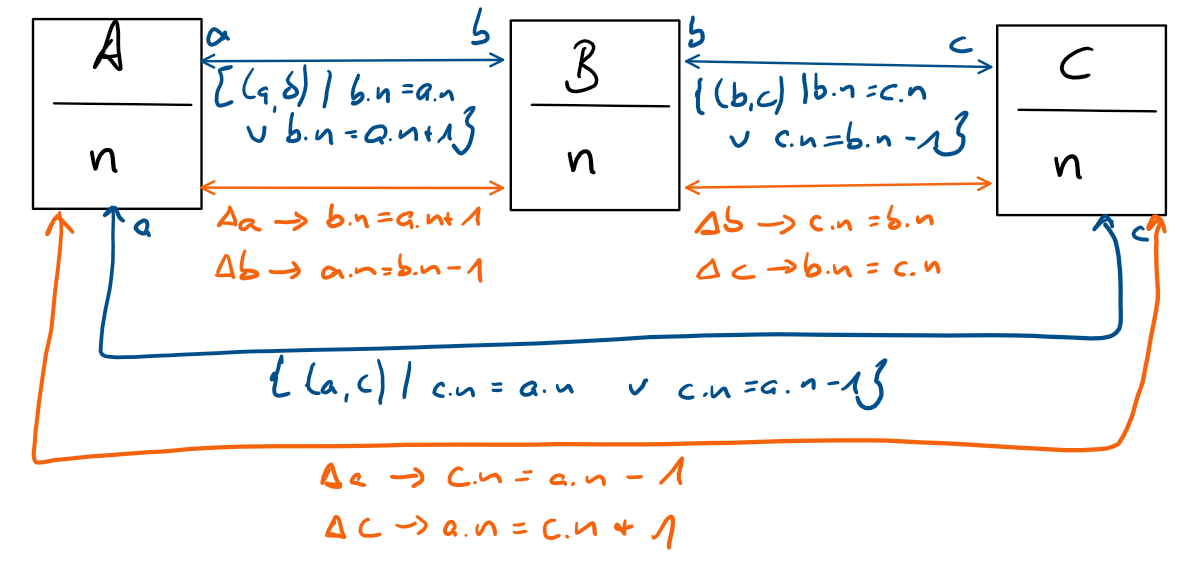
\includegraphics[width=\textwidth]{figures/correctness/formal/divergence_example.png}
%     \caption{Example for divergence}
%     \label{fig:formal:noexecutionorder}
% \end{figure}

% Although we will discuss restrictions to relations and transformations that reduce the chance that no solution can be found, it will not be possible to ensure that such a solution can always be found. This is due to the reason that transformations can perform arbitrary changes given the transformations Turing-completeness, which should not be restricted, because it is unclear which restrictions could be made without forbidding scenarios that should actually we supported. Thus, we assume that transformations are Turing complete.

% Finally, this makes it necessary that a function that applies \modellevelconsistencypreservationrules may not find an execution order that returns a consistent model, thus is should be able to also return $\bot$ as an indicator for that situation.

% We first give a basic definition for such a function without further specifying in which cases the function is expected to return a result other than $\bot$.

% \begin{definition}[Consistency Preservation Application Function]
%     \todo{Define for transformations instead?}
%     Let $\consistencypreservationruleset{}$ be a set of consistency preservation rules for a set of consistency relations $\consistencyrelationset{CR}$ on metamodels $\metamodeltuple{M} = \tupled{\metamodelsequence{M}{n}}$.
%     A consistency preservation application function $\consistencyappfunction{\consistencypreservationruleset{}}$ for these rules is function:
%     \begin{align*}
%         &
%         \consistencyappfunction{\consistencypreservationruleset{}} : (\metamodeltupleinstanceset{M}, \changeuniverse{\metamodeltuple{M}}) \rightarrow (\metamodeltupleinstanceset{M})
%     \end{align*}
%     The function takes a consistent tuple of models and a tuple of changes that was performed on them and returns a changed tuple of models by acquiring changes from the consistency preservation rules in $\consistencypreservationruleset{}$. Thus, it has to fulfill the following conditions:
%     {\setlength{\mathindent}{0em}
%     \begin{align*}
%         &
%         \consistencyappfunction{\consistencypreservationruleset{}}(\modeltuple{m}, \changetuple{\metamodeltuple{M}}) = 
%         \begin{cases}
%             \modeltuple{m'}, & \begin{array}{l@{}}
%                 \exists \changetuple{\metamodeltuple{M}}' = \tupled{\change{\metamodel{M}{1}}', \dots, \change{\metamodel{M}{n}}'} \in \changeuniverse{\metamodeltuple{M}} :\\
%                 \exists \consistencypreservationrule{1}, \dots, \consistencypreservationrule{m} \in \consistencypreservationruleset{} : \\
%                 \cprgeneralizationfunction{\consistencypreservationrule{1}} \concatfunction \dots \concatfunction \cprgeneralizationfunction{\consistencypreservationrule{m}}(\modeltuple{m}, \changetuple{\metamodeltuple{M}}) = (\modeltuple{m}, \changetuple{\metamodeltuple{M}}') \\
%                 \land \tupled{\change{\metamodel{M}{1}}'(\model{m}{1}), \dots, \change{\metamodel{M}{n}}'(\model{m}{n})} = \modeltuple{m'} 
%             \end{array} \\
%             \bot, & otherwise
%         \end{cases}
%     \end{align*}
%     }
% \end{definition}

% \begin{definition}[Consistency Preservation Application Function]
%     \todo{Define for transformations instead?}
%     Let $\consistencypreservationruleset{}$ be a set of consistency preservation rules for a set of consistency relations $\consistencyrelationset{CR}$ on metamodels $\metamodeltuple{M} = \tupled{\metamodelsequence{M}{n}}$.
%     A consistency preservation application function $\consistencyappfunction{\consistencypreservationruleset{}}$ for these rules is function:
%     \begin{align*}
%         &
%         \consistencyappfunction{\consistencypreservationruleset{}} : (\metamodeltupleinstanceset{M}, \changeuniverse{\metamodeltuple{M}}) \rightarrow (\metamodeltupleinstanceset{M})
%     \end{align*}
%     The function takes a consistent tuple of models and a tuple of changes that was performed on them and returns a changed tuple of models by acquiring changes from the consistency preservation rules in $\consistencypreservationruleset{}$. Thus, it has to fulfill the following conditions:
%     {\setlength{\mathindent}{1em}
%     \begin{align*}
%         &
%         \consistencyappfunction{\consistencypreservationruleset{}}(\modeltuple{m}, \changetuple{\metamodeltuple{M}}) = 
%         \begin{cases}
%             \modeltuple{m'}, & \begin{array}{l@{}}
%                 \exists \changetuple{\metamodeltuple{M}}' = \tupled{\change{\metamodel{M}{1}}', \dots, \change{\metamodel{M}{n}}'} \in \changeuniverse{\metamodeltuple{M}} :\\
%                 \exists \consistencypreservationrule{1}, \dots, \consistencypreservationrule{m} \in \consistencypreservationruleset{} : \\
%                 \cprgeneralizationfunction{\consistencypreservationrule{1}} \concatfunction \dots \concatfunction \cprgeneralizationfunction{\consistencypreservationrule{m}}(\modeltuple{m}, \changetuple{\metamodeltuple{M}}) = (\modeltuple{m}, \changetuple{\metamodeltuple{M}}') \\
%                 \land \tupled{\change{\metamodel{M}{1}}'(\model{m}{1}), \dots, \change{\metamodel{M}{n}}'(\model{m}{n})} = \modeltuple{m'} 
%             \end{array} \\
%             \bot, & otherwise
%         \end{cases}
%     \end{align*}
%     }
% \end{definition}



% \begin{definition}[Correct Consistency Preservation Application Function]
%     Let $\consistencyappfunction{\consistencypreservationruleset{}}$ be a consistency preservation application function for a set of \modellevelconsistencypreservationrules $\consistencypreservationruleset{}$ for a set of \modellevelconsistencyrelations $\consistencyrelationset{CR}$.
%     We say that:
%     \begin{align*}
%         &
%         \consistencyappfunction{\consistencypreservationruleset{}} \mathtext{is correct} \equivalentperdefinition \\
%         & \formulaskip
%         \forall \modeltuple{m} \in \metamodeltupleinstanceset{M} : \forall \changetuple{\metamodeltuple{M}} = \tupled{\change{\metamodel{M}{1}}, \dots, \change{\metamodel{M}{n}}} \in \changeuniverse{\metamodeltuple{M}} :
%         \modeltuple{m} \consistenttomath \consistencyrelationset{CR} \Rightarrow \\
%         & \formulaskip
%         \consistencyappfunction{\consistencypreservationruleset{}}(\modeltuple{m}, \changetuple{\metamodeltuple{M}}) \consistenttomath \consistencyrelationset{CR}
%     \end{align*}
% \end{definition}




Now it is obvious that the consistency preservation rules can actually do anything to achieve consistency, including returning always the same set of models that is consistent, although that may not be expected. We will discuss later which reasonable assumptions can be made to the behavior to on the hand not restrict the possibilities of the transformation developer and on the other hand be able to ensure some properties of the transformations and their execution.

\todo{First restriction: Input delta of APP only contains changes to one model -> no synchronisation}
\todo{Second restriction: Input delta is not rejected}
\todo{Third restriction: Generated deltas are monotone}

From a theoretical perspective, it is always possible to a specify consistency relations according to the definition, as it is just a subset of elements.
It is also always possible to define a consistency preservation rule for a consistency relation according to its definition, as can simply return any any element of the relation.
\todo{This is not true: the source model may not be in the relation, then its not possible, at least with the current definition. With a synchronizing transformation, any modification can be made to both models, then its fine.}
The generalization function is generic, so it can always be applied.
Finally, the consistency preservation application function is an artifact that cannot be easily specified according to the definition for a given set of consistency preservation rules.
It is always possible to have a set of consistency preservation rules for which no application function can be defined that returns a consistent result for at least one input model and change tuple, as there is not sequence of consistency preservation rules that achieves that.
\todo{Example!}
Even worse, the problem to define such a function is Turing-complete, which makes it impossible to decide whether such a function exists.
\todo{Show Turing-completeness}
Consequence: From a theoretical perspective, this function is the crucial part!

Essential problem: One transformation may restore consistency between A and B and another between A and C. If then a transformation restores consistency between B and C, the resulting B' and C' may not be consistent A anymore.

Alternative to an app function: Define a \emph{well-definedness} property for a set of transformations, requiring that they can be executed in any order to always terminate consistently. However, this is a very strict requirement, which can usually not be fulfilled, so we do not further investigate that.
\todo{Give simple example why that does not work.}


Best-behaved app function: Whenever there is a sequence of CPRs, the app function finds item. This is still not possible due to Turing-completeness. The function would need to decide whether the network terminates or not.

Only achievable app function is a best-effort (i.e. conservative) function: A function that either returns a consistent set of models or that does return bottom. Not making a statement about how often a correct result is returned in comparison to how often it is possible.

This approach is conservative. The question is then, how high the degree of conservativeness is. In the worst case, a function that always returns bottom would fulfill the definition, but that is not what we want. We want to reduce conservativeness.

Goal: Find a solution in as many cases as possible, abort in the others (conservatively). There are two subgoals to achieve that:
1. Function must be correct, i.e. always terminate (no endless sequence of CPR) and terminate in a consistent state
2. Function must be as less conservative as possible

It is clear that we cannot give a closed function for APP that just by a given change returns a sequence of CPR that results in a consistent state. APP has to be calculated dynamically during execution. Therefore we consider it as an algorithm in the following.


\subsection{Achieving a Correct Application Function}
\todo{These problem cannot occur if a function fulfills the definition, because it always finds a sequence. So the question is how to fulfill the definition.}

It is easy to achieve that the APP function only terminates in a consistent state, because knowing the relations allows to check whether all relations are fulfilled. 
\todo{Need to define that a transformation may not be able to process a specific change? Then there could be inconsistent terminiation because a transformation cannot be executed anymore.}

Problems due to which the function does not terminate: Alternation and Divergence

Alternation: Run through same state twice
Divergence: Always produce new states without reaching a consistent state

Two possibilities to avoid problems:
1. Make assumptions to transformations that avoid them
2. Detect them dynamically and abort


\subsubsection{Avoiding Alternation / Divergence}

Making assumptions that avoid them is rather hard, as we will show in the following.

\paragraph{Idea:} Require monotony to avoid alternation

We would have to relax the definition of transformation to be monotone, because if a transformation is monotone, it may only append information, but this is not always possible, as can be seen in the following example. A monotone transformation must be able to return bottom if it cannot make further changes to restore consistency to the relation.

\begin{definition}[Monotone Transformation]
    Transformation gets models M and deltas D and produces new deltas D'. Taking the union of the original models M and the new models D'(M), then D(M) must be a subset of that, because other elements would have been added and removed afterwards or elements would have been changes once by D and again in a different way by D'.

    Generally, monotony could also mean that only the same complete model state is not passed twice. \todo{Why dont we do that?}
\end{definition}

This would mean that each transformation only appends changes, i.e., if an element was added/removed, the transformation may not do the inverse. The same applies to attribute/reference changes: if an attribute/reference was already changes it may not be changed again.
This way, it is by design impossible to pass through the same state again. Actually, if a monotone transformation returns bottom, the network has to terminate with a failure.
However, this is hard restriction to transformations. It leads to the fact that in some networks that actually have a simple solution no solution is found at all. This can be easily seen at the example in \autoref{fig:formal:monotonycounterexample}. In the example adding "aa" to the left model, any execution order of the transformations leads to the situation that a previous change must be revoked to result in a consistent state. However, it is possible to derive a consistent state for that input change.

\begin{figure}
    \centering
    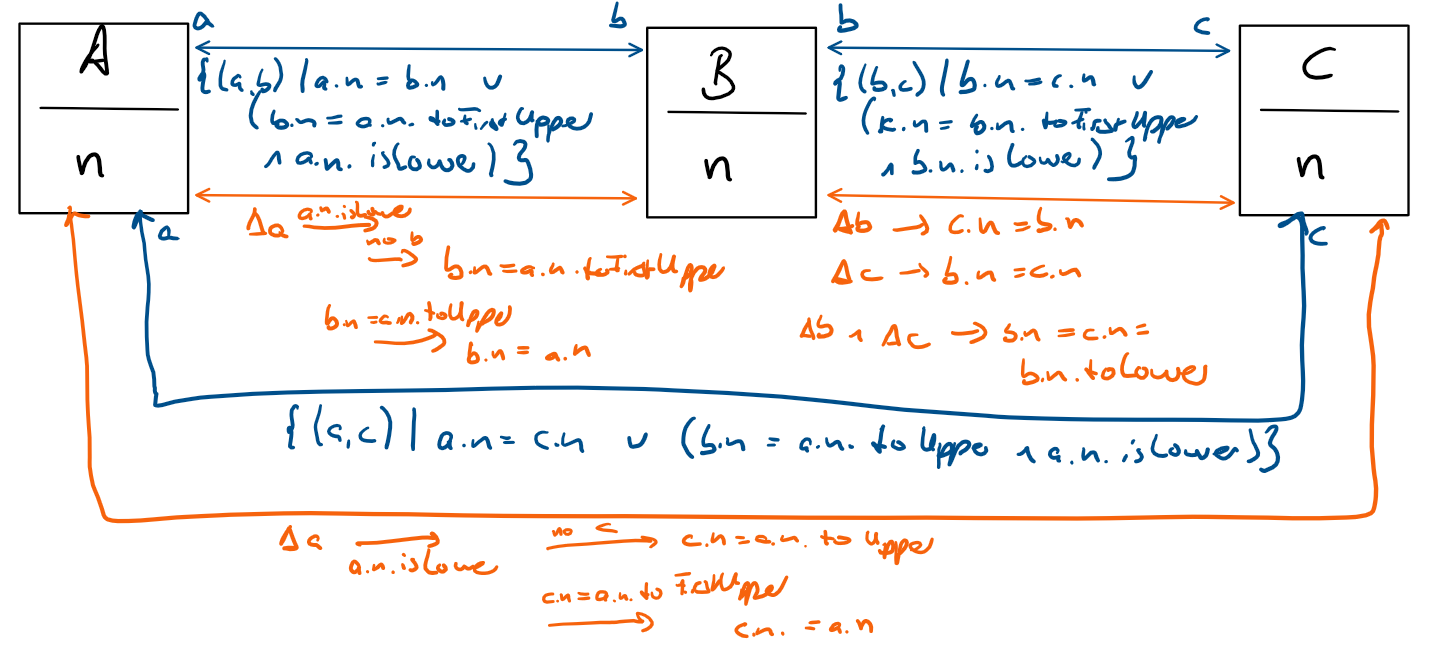
\includegraphics[width=\textwidth]{figures/correctness/formal/monotony_counterexample.png}
    \caption{Counterexample for monotony}
    \label{fig:formal:monotonycounterexample}
\end{figure}

One could now argue that there are binary relations in the example, which may never be fulfilled at all. We will later discuss how far relations that cannot be fulfilled should be restricted. However, in general, this is wanted behavior, because in general it may be necessary that transformations produce intermediate states that are not yet consistent with each other. Otherwise this would means that each transformation is always able to directly deliver a state that is consistent to all other relations, which is especially not possible, because other transformations may add further information to the models. More precisely, a relation may consider <a model consistent to all other models that contain any additional information not affected by the transformation. For example, a UML class model may be considered consistent to all Java models with any implementation of the specified methods, thus to an infinite number of models. Now saying that it should not be allowed that the transformation selects one with an empty implementation because that is not consistent to another relations induced by another transformation, such as the relationship to a component model, does not make any sense. Thus having those relation elements that may be considered locally consistent but will never occur in a globally consistent tuple of models does not make sense.
In the example, we can see that such an inconsistent intermediate state is passed through and afterwards a consistent tuple of models is reached if not requiring monotony.
In consequence, requiring monotony from transformations is a too strict requirement, because it is necessary to run through states that may be changed later on.

\begin{theorem}
    An application function for monotone transformations either returns a consistent model or produce a sequence of CPRs returning delta that return models of always growing size (i.e. it diverges).
\end{theorem}


\paragraph{Divergence cannot be avoided}

There are rather equal network, one that terminates after a long time and one that never terminates. 
Consider the example. The relations are defined in a way such that for any allocation for any of them a consistent tuple of models can be found. However, the transformations are not able to find it because they make "bad" choices from a set of choices that are conflicting. 
This can be seen in the example in \autoref{fig:formal:divergenceexample}.

\begin{figure}
    \centering
    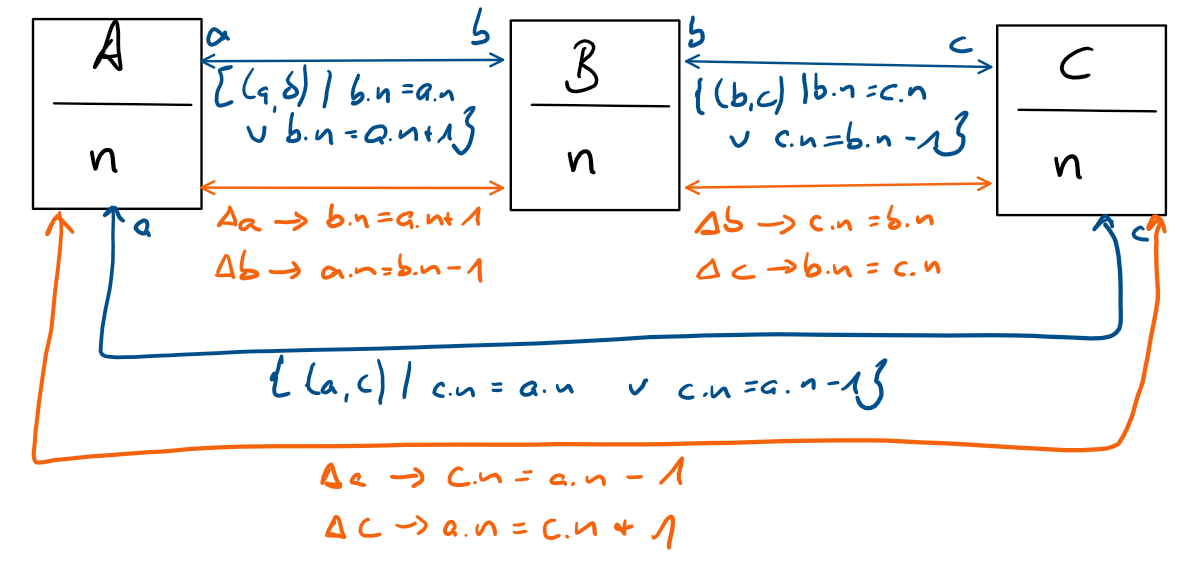
\includegraphics[width=\textwidth]{figures/correctness/formal/divergence_example.png}
    \caption{Example for divergence}
    \label{fig:formal:divergenceexample}
\end{figure}

Thus, systematically avoiding divergence is not possible. 



\paragraph{Detecting Alternation / Divergence}

In consequence, we propose to dynamically deal with alternation / divergence.
To detect alternations, the execution can simply track if a state way already processed. Apart from spatial problems, this does always work.
Finding divergence is not that easy, because it is generally not possible to define an upper bound for the number of executions of a single transformation.
This is due to the reason that, again, this conflicts with the Halting problem.
We can see this at the simple example in \autoref{fig:formal:noupperboundexample}.

\begin{figure}
    \centering
    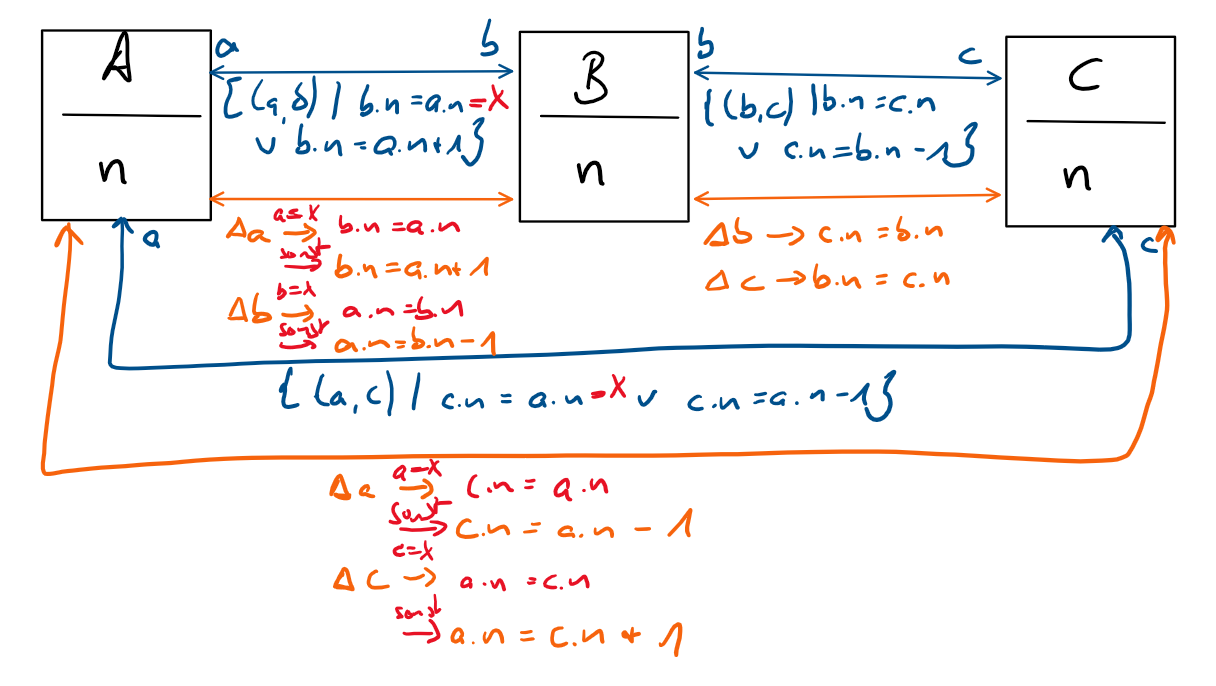
\includegraphics[width=\textwidth]{figures/correctness/formal/no_upper_bound_example.png}
    \caption{Example for no upper bound}
    \label{fig:formal:noupperboundexample}
\end{figure}

Depending on the value X, the transformations have to be executed X times to result in a consistent state. This value can be arbitrarily chosen, thus an arbitrary number of executions may be necessary to terminate in a consistent state.

From an engineering perspective, this is still unwanted behavior. We claim that a transformation network that takes thousands of executions of the same transformation to find a consistent state works not as expected and if running into a failure would expose severe problems to find the reasons for that failures.
Thus, we propose to simply abort the execution after some time to be sure not to run in an endless loop.

Finally, this problem is comparable to ordinary programming, because there the same situations regarding alternation and divergence can occur that result in non-termination of a program.
As we all know, it is impossible to systematically avoid that, but just possible to carefully develop the program and apply best practices to avoid such situations.

In the following, we propose measures to reduce the number of cases in which problematic cases can occur.
In a case study, we will see that using such measures already resolves most of the problems that can occur.
Additionally, we propose an orchestration strategy that improves the possibility to find errors in case something goes wrong.

\textbf{Central insight:} Alternation / Divergence cannot be avoided systematically (like in ordinary programming), if not restricting transformations in a way that may not be reasonable.




\subsection{Reducing Conservativeness of the Application Function}

Goal: Find a solution in as many cases as possible, abort in the others (conservatively). There are two approaches to achieve that: 
1. Reduce the number of cases in which there is no solution by adding assumptions to the relations and transformations (restrict input of app function)
2. Improve the ability to find a solution if it exists (improve capabilities of app function)
Secondary goal: In cases, in which no solution is found, support the user in understanding why no solution was found.


Regarding 1: Reduce problematic cases


1. reduce cases in which there is no such solution
1.1. On relation level: Only sets, so analysis possible.
Ensure that relations are defined in a way such that they do not allow a locally correct set of CPRs that has no APP solution. If there is a pair of models (or elements of a fine-grained relation) in a relation, a CPR may return it. But if there is no consistent tuple of models containing these two, it does not make any sense to consider these elements (even worse, if we have monotony, adding these elements makes the network unsolvable). For that reason, we need compatibility. Avoids both alternation and divergence
1.2. On transformation level: Hard to perform analyses
Require monotony to avoid alternation
Give some example why divergence cannot easily be avoided, thus terminate at some point
2. find the solution in as many cases as possible -> reasonable orchestration strategy
Focus on engineering solution 


Thus, there arise two questions:
- Although theoretically easy, how to practically define a CPR that is synchronizing?
- How to define an APP function and which requirements does that impose?












Two levels of correctness:
\begin{enumerate}
    \item Local correctness: a consistency relation is correct to the global relation and the CPR is to the relation, i.e. given two models and changes in them, the transformation can produce a change that restores consistency regarding the global consistency relation of these two models (i.e. there are some other models with which these two models would be consistent regarding the global specification) --> a network is locally correct, if this property is fulfilled
    \item Global correctness: the binary relations together are equal to the global one and the execution function is able to find consistency models after a change to initially consistent models --> network is globally correct, if this property is fulfilled
\end{enumerate}
Potentiell ist lokale Korrektheit (zumindest einer CPR zu ihrer CR per Konstruktion) herstellbar -- das war auch das Ergebnis bisheriger Studien --, eventuell auch von einer CR zu einer globalen CR, obwohl die ja eigentlich meist nicht existiert, daher nehmen wir das als gegeben an.
Dann zeigen, dass die globale Beziehung der Relationen nicht äquivalent ist zu den einzelnen lokalen, daher kommt hier zusätzliche Komplexität rein (Kompatibilitätsbegriff).
Final muss noch die Ausführungsfunktion korrekt sein, hier aber Problem der Turing-Vollständigkeit. 
Daher Einschränkungen an Transformationen finden bzw. ingenieurmäßige Ausführungsreihenfolge festlegen, die möglichst oft richtige Lösungen findet und sonst konservativ mit einem Fehler terminiert.


\textbf{On top of ordinary bx correctness:}
\begin{itemize}
    \item Transformations need to be synchronizing
    \item Consistency relations need to fulfill a notion of correctness
    \item Exkurs:
    \begin{itemize}
    \item Is compatibility a subclass of correctness? Is every correct set of relations compatible as well?
    \item Problematisch: unser Konsistenzbegriff für Relationen (feingranulare Relationen) schließt keine Modelle aus, der Konsistenzbegriff hier aber schon. Wie realisiere ich die feingranularen Relationen, die dafür sorgen, dass nur genau ein Tupel von Modellen konsistent ist?
    \item Wir müssen bei der Ableitung unseres Kompatibilitätsbegriffes erklären, dass bei uns der vollständige Ausschluss bestimmter Modelle nicht Teil einer feingranularen Konsistenzrelation sein darf, sondern Teil einer weiteren Spezifikation, die angibt, welche Modelle überhaupt valide sind. Denn so ist es in Transformationssprachen tatsächlich auch.
    \end{itemize}
    \item Execution function needs to be defined, which potentially induces requirements to the transformations.
\end{itemize}


Annahmen:
\begin{itemize}
    \item Nutzeränderungen dürfen nicht rückgängig gemacht werden.
    \item Nutzeränderungen lassen sich so feingranular zerlegen, dass, falls durch die Erzeugung/Änderung eine Konsistenzrelation verletzt wird, es in jeder unabhängigen Teilmenge von Konsistenzrelationen eine verletzte Konsistenzrelation gibt, für die die geänderten Elemente einem Condition Elemente entsprechen, es also insbesondere keine Teilmenge der geänderten Element gibt, die bereits dieses Condition Element sind. Ansonsten ist durch unsere Kompatibilitäts-Definition nicht sichergestellt, dass eine konsistente Modellmenge gefunden werden kann.
\end{itemize}

Voraussetzungen:
\begin{itemize}
    \item Relationen müssen korrekt sein, d.h. sie müssen bzgl. einer globalen (meist eher implizit bekannten) n-ären Relation zwischen allen Modellen identisch sein. Eine n-äre Relation lässt sich nicht immer zerlegen (siehe Stevens), aber wir nehmen das an.
    \item Die einzelne Transformation muss bzgl. ihrer Relation korrekt sein, d.h. sie muss bei Änderungen in beiden Modellen ein zur Relation konsistentes Modell liefern.
\end{itemize}

Ebenen der Korrektheit:
\begin{itemize}
    \item Relationen müssen korrekt sein, d.h. gegeben eine Nutzeränderung muss es überhaupt möglich sein eine konsistente Menge an Modellen zu finden. Wenn Transformationen etwas beliebigen tun dürfen geht das immer. Wir nehmen an, dass eine Nutzeränderung nicht rückgängig gemacht werden soll (bzw. wenn sie rückgängig gemacht werden würde eigentlich die Änderung invalide war, d.h. keine Konsistenz im Netzwerk hergestellt werden kann). Daher sind Relationen nur korrekt, wenn für fixierte Elemente, die durch eine Nutzeränderung entstehen können, eine Modellmenge abgeleitet werden kann, die bzgl. der Relationen konsistent ist. D.h. gegeben einige Elemente muss es eine Modellmenge geben, die in allen Relationen liegt und die diese Elemente enthält (-> Kompatibilitätsbegriff). Wir betrachten in Kapitel ?, wie man Kompatibilität präzise definieren und feststellen/garantieren kann.\\
    Resultat: Gegeben eine Änderung ist es möglich eine Transformation anzugeben, die aus der Änderung ein konsistentes Modell produziert.
    \item Einzelne Transformationen müssen korrekt sein: Wir fordern Korrektheit der Transformation sowieso. Allerdings machen in einem Netzwerk verschiedene Transformationen Änderungen an allen Modellen, d.h. wir müssen nicht den "normalen" Transformationsfall unterstützen, dass Deltas in einem Modell ins andere übertragen werden, um Konsistenz herzustellen, sondern die Transformationen müssen \emph{synchronisierend} sein, also Deltas in beiden Modelle annehmen und dann Konsistenz herstellen. Wir definieren diese Synchronisationseigenschaft und betrachten in Kapitel ?, welcher zusätzlichen Anforderungen sich dadurch bzgl. EMOF-Modellen ergeben. Der Input sind Deltas in zwei Modellen, und einzelne Deltas sind potentiell als "authoritative" definiert, was bedeutet, dass die erzeugten/geänderten Elemente nicht noch einmal geändert/gelöscht werden dürfen. Das realisiert die Anforderung, dass Nutzeränderungen nicht rückgängig gemacht werden dürfen. \\
    Resultat: Gegeben Änderungen in zwei Modellen (mit potentiell authoritativen Änderungen) gibt die Transformation ein konsistentes (bzgl. der Konsistenzrelation) Modellpaar zurück. 
    \item Korrektheit der Anwendungsfunktion: Die Anwendungsfunktion muss die Transformationen in einer 
\end{itemize}

Annahme an Transformationen:
\begin{itemize}
    \item Muss eine Transformation mit jedem beliebigen Delta umgehen können müssen? Eine Einschränkung auf Monotonie würde dies verhindern. Bzw. wir müssten zeigen, dass es Konsistenzrelationen gibt, die unter der Anforderung an Monotonie nicht wiederhergestellt werden können. Bspw. fügt eine andere Transformation 3 Elemente hinzu, wo zwei mit dem anderen entsprechend der Konsistenzrelationen korrelieren und somit keine Witness-Struktur aufgebaut werden kann, die Konsistenz beweist. Das lässt sich durch Hinzufügen weiterer Elemente potentiell nicht auflösen (siehe Beispiele im SoSym-Paper).
\end{itemize}

\todo{Überlegen, wo hier die Definition von (undirektionalen Relationen) rein muss.}
Präzisere Eigenschaften:
\begin{itemize} 
    \item Synchronisationseigenschaft: Eine Transformation kann mit Änderungen an mehreren Modellen umgehen, d.h. gegeben zwei konsistente Modelle + Änderungen an beiden resultiert in zwei Modellen, die konsistent bzgl. der Relation(en) zwischen den Metamodellen sind
    \item 
\end{itemize}  

\begin{itemize}
    \item Kompatibilität entsprechend Modularisierungsebene
    \item Synchronisation auf Operationalisierungsebene: Abwägen, dass eine Transformation verschiedene Zustände sehen könnte, auf denen sie ausgeführt wird. Aber letztendlich muss sie damit klarkommen, dass zwei Modelle geändert wurden. 
\end{itemize}

TODO:
\begin{itemize}
    \item Authoritative Modelle (bzw. eher authoritative Regionen) diskutieren (Verweis Stevens)
\end{itemize}



\section{Local Correctness}

Simple solution: we define a transformation which normatively implies a relation, thus it is correct by construction. From a theoretical perspective this is easy to reach, from a practical it is not.
However, in contrast to our definition of synchronizing transformations, ordinary transformations are only able to process changes in one model and update the other accordingly. Together with the assumption that both models were consistent before does not fit with our scenario, because if one model is modified, the other may be modified as well by another transformation across another path, before a transformation is executed. Thus, both models may have been modified.
We consider the following situation: Models A and B were consistent. Model A was changed an we have the changes at hand. Additionally, B was modified because there were other changes propagated through the network. 
We distinguish all cases of modifications to B that may have violated a consistency relation between A and B (according to our fine-grained consistency notion) and consider what we have to do there (e.g. find-or-create-pattern).
Put empirical analysis here.


\section{Correct APP function}

We make the following approach: Always assume there is a solution and start executing the transformation (for now in any order). Finally, the network has to terminate at a fixed point. We investigate, what the reasons may be that it does not try to avoid them.

These reasons can lie in the relations:
- relations cannot be completely unfulfillable, as the empty models are always consistent, thus there can always be CPRs that result in a consistent set of models
- however, if relations contain pairs that can never be in any consistent model tuple they improve proneness to errors, because a CPR may return that pair, which will never fit to any result of any other transformation. Thus, this should not be allowed -> compatibility

These reasons can also lie in the transformations:
- Transformations can make choices and they make choices that are always incompatible to other (refer to example)

Essentially there are two problems: alternation and divergence



\subsection{Other thought}
If each element occurs in each relation only once (so always 1:1 mappings) and if we have compatibility, then any transformation order would return exactly the one model tuple that fits.
However: In that case we would have confluence, every information must directly be available in B from A without a transitive propagation over C. This is not what we want. So there must in general be more than one option a transformation is fine with that to reflect the information that another transformation may add or change.


\todo{Hippocraticness is not necessary but needs to be discussed}

Goal:
- Find a solution in as much cases as possible, abort in the others (conservatively)
- To do so: reduce cases in which there is no such function
- To do so: ensure that relations are defined in a way such that they do not allow a locally correct set of CPRs that has no APP solution. If there is a pair of models (or elements of a fine-grained relation) in a relation, a CPR may return it. But if there is no consistent tuple of models containing these two, it does not make any sense to consider these elements (even worse, if we have monotony, adding these elements makes the network unsolvable). For that reason, we need compatibility.
- 

\chapter{Proving Compatibility of Consistency Relations
    \pgsize{90 p.}
}
\label{chap:compatibility}

%\todo{Check whether we can better derive necessity of compatibility in terms of transformations to being able to find consistent models at all. Does only ensure that transformations can at least, if properly defined, find consistent models.}
\todo{Final müssen wir diskutieren, wie sich Inkompatibilitäten darauf auswirken, ob eine Ausführungsstrategie einen konsistenten Zustand findet. Im Optimalfall zeigen wir, dass Kompatibilität das Orchestrierungsproblem vereinfacht!}
\todo{Prüfen, ob diskutiert ist, dass mit Kompatibilität sichergestellt wird, dass eine feingranulare Änderung immer zu einem konsistenten Modellset führen kann, was diese Änderung reflektiert.}
\todo{Wir müssen noch unterstützen, dass Konsistenzrelationen die Existenz von Objekten ausschließen: Wenn ein Student vorhanden ist, darf kein Employee mit gleichem Namen vorhanden sein (da Studis nicht arbeit dürfen). Das geht nicht mit der naiven Verallgemeinerung, die sagt, dass dann die Modelle selbst eingeschränkt werden müssen, da das Modell mit dem Employee i.A. erlaubt ist, nur nicht, wenn ein Student mit dem Namen vorhanden ist.}

\mnote{Artifacts and correctness in modular consistency specification}
We have defined in \autoref{chap:correctness} that transformations are composed of \glspl{consistency relation} and \glspl{consistency preservation rule} that preserve them.
We especially focus on binary relations and according preservation rules, which concern two metamodels.
Multiple transformations can be combined to a network with an orchestration and application function that executes the transformation in a determined order to restore consistency after changes to concrete models.
We have also identified correctness notions and came to the conclusion that with modular, binary transformations combined to a network the individual consistency preservation rules must be correct with respect to the consistency relations they preserve and the orchestration and application functions must be correct with respect the combination of all consistency relations, such that all models are consistent to all consistency relations after executing the transformations.

\mnote{Consistency relations are correct by construction}
As a consequence of the identified correctness notion, we also found that the underlying consistency relations themselves can, from a theoretical perspective, be considered correct by construction, as there is no other artifact (be it explicit or only implicitly given) with respect to which it has to be correct.
Since we assume transformations to be developed independently and reused in a modular way, we can especially not assume a monolithic consistency relation to which the modular consistency relations must be correct (cf.\ \autoref{chap:correctness:notions_correctness:dimensions}).
We have, however, already given examples for cases in which binary consistency relations are somehow contradictory.
This is the case if the developers of the individual transformations have different, conflicting notions of consistency between the metamodels.
In the worst case, this can lead to the situation that no single set of models would be considered consistent to a set of binary consistency relations, which is obviously unwanted behavior.
We have discussed an abstract example for that case already in \autoref{chap:correctness:notions_correctness:relations}.

\begin{figure}
    \centering
    %% From motivational_example in MPM4CPS paper

\newcommand{\hdistance}{14em}
\newcommand{\classwidth}{6em}

\begin{tikzpicture}

% Person
\umlclassvarwidth{person}{}{Person\sameheight}{
firstname\\
lastname\\
address\\
income
}{\classwidth}

% Employee
\umlclassvarwidth[,above right=2em and \hdistance of person.east, anchor=south]{employee}{}{Employee\sameheight}{
name\\
socsecnumber\\
salary
}{\classwidth}

\umlclassvarwidth[,below=4em of employee.south, anchor=north]{resident}{}{Resident\sameheight}{
name\\
address\\
socsecnumber
}{\classwidth}


% CONSISTENCY RELATIONS
\draw[consistency relation] (person.north) |- node[pos=0, above left] {$p$} node[pos=0.75, above] {$\consistencyrelation{CR}{PE}$} node[pos=1, above left] {$e$} (employee.west);
\draw[consistency relation] (employee.south) -- node[pos=0, below left] {$e$} node[right, align=left] {$\consistencyrelation{CR}{ER}$ / $ \consistencyrelation{CR}{ER}'$}% /\\ $R'_{ER}$} 
node[pos=1, above left] {$r$} (resident.north);
\draw[consistency relation] (resident.west) -| node[pos=0, below left] {$r$} node[pos=0.25, below] {$\consistencyrelation{CR}{PR}$ / $\consistencyrelation{CR}{PR}'$} node[pos=1, below left] {$p$} (person.south);

\node[consistency related element, below left=5em and 2em of person.south west, anchor=north west] {
$\begin{aligned}
    \consistencyrelation{CR}{PE} =\; &
        \setted{\tupled{p,e} \mid %\\
        %& 
        \mathvariable{p.firstname} + "\text{\textvisiblespace}" + \mathvariable{p.lastname} = \mathvariable{e.name}%\\
        %& 
        \land \mathvariable{p.income} = \mathvariable{e.salary}
    }\\[0.3em]
    \consistencyrelation{CR}{PR} =\; &
        \setted{\tupled{p,r} \mid %\\
        %& 
        \mathvariable{p.firstname} + "\text{\textvisiblespace}" + \mathvariable{p.lastname} = \mathvariable{r.name}%\\
        %& 
        \land \mathvariable{p.address} = \mathvariable{r.address}
    }\\
    \consistencyrelation{CR}{PR}' =\; &
        \setted{\tupled{p,r} \mid %\\
        %& 
        \mathvariable{p.lastname} + ",\text{\textvisiblespace}" + \mathvariable{p.firstname} = \mathvariable{r.name}%\\
        %& 
        \land \mathvariable{p.address} = \mathvariable{r.address}
    }\\[0.3em]
    \consistencyrelation{CR}{ER} =\; &
        \setted{\tupled{e,r} \mid %\\
        %& 
        \mathvariable{e.name} = \mathvariable{r.name} %\\
        %& 
        \land \mathvariable{e.socsecnumber} = \mathvariable{r.socsecnumber}
    }\\
    \consistencyrelation{CR}{ER}' =\; &
        \setted{\tupled{e,r} \mid %\\
        %& 
        \mathvariable{e.name.toLower} = \mathvariable{r.name} %\\
        %& 
        \land \mathvariable{e.socsecnumber} = \mathvariable{r.socsecnumber}
    }
\end{aligned}$
};

\end{tikzpicture}
    \caption[Three metamodels with (in)compatible consistency relations]{Derivation of \autoref{fig:networks:three_persons_example}: Three simple metamodels for persons, employees and residents, and three binary relations $R_{PE}, R_{PR}, R_{ER}$ between each pair of them, with $R'_{PR}$ as an alternative for $R_{PR}$ and $R'_{ER}$ as an alternative for $R_{ER}$.}
    \label{fig:compatibility:three_persons_example_extended}
\end{figure}

\mnote{Intuitive compatibility in the running example}
We recapture the running example defined in \autoref{fig:networks:three_persons_example} and extend it with alternatives for two of the binary consistency relations in \autoref{fig:compatibility:three_persons_example_extended}.
The example contains three pairwise consistency relations between persons, employees and residents and are defined in a way such that none of them can be omitted, because each pair shares a unique overlap in their attributes.
In that example, the consistency relations $R_{PE}, R_{PR}$ and $R_{ER}$ are fulfilled if for any person (and analogously employee and resident) in the models there is exactly one employee and one resident, which fulfill the relations for names and further attributes defined by the consistency relations.
As we will see later, it is of special importance that there is always only one such corresponding element, e.g., that there are not two employees fulfilling the relation to a single resident.
Intuitively, these consistency relations are \emph{compatible}, as they lead to a reasonable set of models that are considered consistent to each other.

\begin{figure}
    \centering
    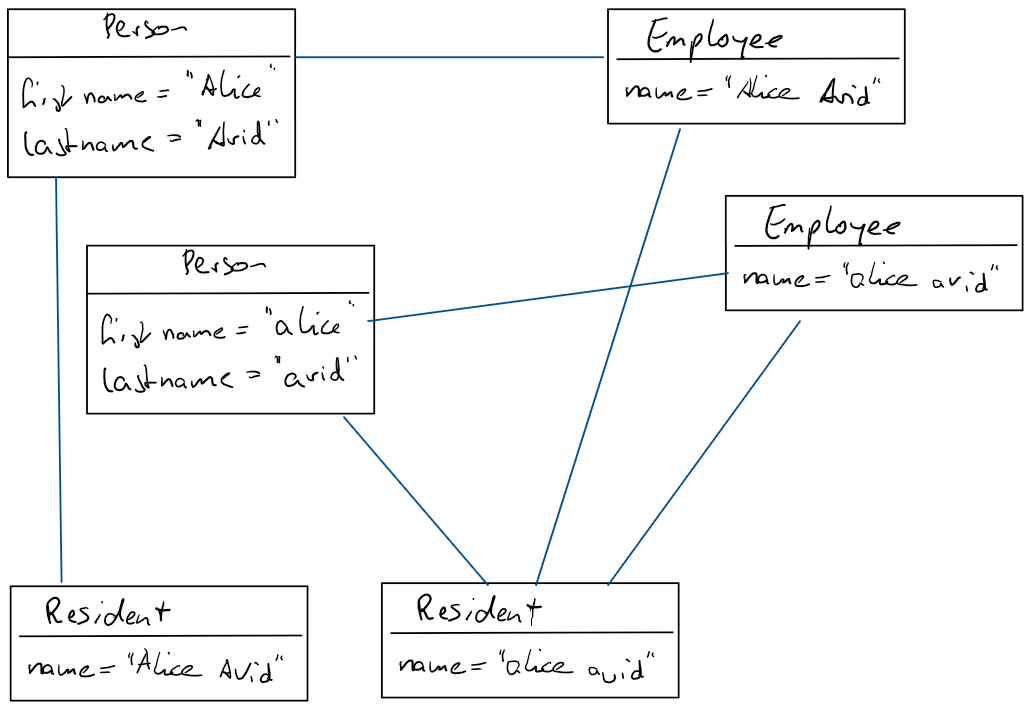
\includegraphics[width=\textwidth]{figures/correctness/compatibility/intuitive_incompatibility.png}
    \caption[Example for an intuitive notion of incompatibility]{Elements required by the consistency relations in \autoref{fig:compatibility:three_persons_example_extended} for a resident with the name \enquote{Alice Avid}.}
    \label{fig:compatibility:intuitive_incompatibility}
\end{figure}

\mnote{Intuitive incompatibility in the modified running example}
In contrast, considering consistency relation $R'_{PR}$ instead of $R_{PR}$, the relations can never be fulfilled, because the concatenation of $firstname$ and $lastname$ from person to employee and from person to resident is conflicting.
The relation between employees and residents assumes to be $firstname$ and $lastname$ to be concatenated in the same order, whereas the relations to person do not.
Fulfilling these relations would require an infinitely large model, as each cycle through the relations swaps $firstname$ and $lastname$ and appends an additional comma due to the relation between person and resident.
Thus, the set of consistent model tuples would be empty.

\todo{Maybe leave the following out, or move it to the more fine-grained part}
\mnote{More detailed incompatibility in the modified running example}
In addition, considering consistency relation $R'_{ER}$ instead of $R_{ER}$, no models containing residents with a name not written in lower case can be consistent to all relations, as depicted in \autoref{fig:compatibility:intuitive_incompatibility}, which, for reasons of simplicity, omits all other attributes than the names.
A resident with a non-lower-case name requires a person with equally written first and last name to exist.
This, in consequence requires an employee with an equally written name to exist.
The relation $R'_{ER}$ now requires a resident with the name written in lower case to exist, which again requires a person with the lower-case name and this, in turn, requires an employee with the lower-case name.
In consequence, however, the resident with the lower-case name would correspond to both the employee with the original and the lower-case name, whereas the resident with the original name does not correspond to any employee.
More intuitively speaking, it is impossible to find an employee that fulfills the consistency relation $R'_{ER}$ for a resident with a non-lower-case name.
This is what we will call and later precisely define as an \emph{incompatibility} of the consistency relations, as they define constraints that cannot be fulfilled at the same time.
This can always occur if there is a cycle in the graph induced by the combined consistency relations.

\mnote{Incompatibilities prevent transformations from finding consistent models}
On the one hand, such incompatibilities are unwanted, as they indicate that developers have different, contradictory notions of consistency.
On the other hand, the contradictions can easily lead to the situation that the transformations are not able to find consistent models or at least that their orchestration for finding consistency models becomes unnecessarily difficult.
Therefore, in this chapter we first discuss some scenarios to identify an intuitive notion of compatibility, which we then use to define a precise notion of \emph{compatibility}.
Afterwards, we develop a formal, inductive approach to prove compatibility of relations, which we base on a formal framework for which we prove correctness and then derive a practical approach for the transformation language \gls{QVTR} that uses that formal framework.
The approach is based on the insight that consistency relations having a specific kind of tree structure are compatible and that removing a specific kind of redundant relations is compatibility-preserving.
This chapter thus constitutes our contribution \contributionref{contrib:correctness:compatibility}, which consists of four subordinate contributions: a discussion of compatibility notions, a formal definition of one such notions, a formal approach to prove compatibility, and finally a practical realization of that approach.
It answers the following research question:

\researchquestionrepeat{rq:correctness:compatibility}

% In this article, we consider the relations defined by bidirectional transformations.
% We clarify the notion of \emph{compatibility} of these relations and develop an approach to prove compatibility of relations in a given network of transformations.
% To achieve this, we formally define a notion of consistency, based on fine-grained consistency relations, as well as compatibility.
% Building on this formalism, we are able to derive an inductive, formal approach for proving compatibility of relations by identifying those that are redundant.
% The essential idea is that if consistency relations have a specific kind of tree structure, we are able to show that they are inherently compatible.
% Furthermore, we show that adding redundant relations to such a tree preserves compatibility.
% In consequence, reducing an arbitrary network of relations to a tree by removing redundant relations proves compatibility.
% Finally, we present an operationalized approach based on that formal approach for \qvtr to prove compatibility of a network of \qvtr relations.
% That approach transforms \qvtr relations into first-oder logical formulae and finds redundant relations by applying an SMT solver.
% % We propose an approach that is able to prove that transformations are compatible, on the example of QVT-R. The approach represents the transformation rules as a graph of metamodel elements with consistency relations between them. Its goal is to find an equivalent set of trees of consistency relations, which are compatible due to the inherent absence of cycles. To achieve that, it decomposes the graph into independent subsets and then removes redundant consistency relations within existing cycles. To prove redundancy of a relation, cycles of relations are transformed into logical expressions and evaluated with an SMT solver. 
% More detailed, we make the following contributions:
% \begin{description}[leftmargin=\parindent]
%     \item[\contributionlabel{contrib:formalization}{Compatibility Formalization}{C1}:] We formalize a notion of consistency and precisely define \emph{compatibility} of relations in a network of transformation.
%     \item[\contributionlabel{contrib:formalapproach}{Formal Approach}{C2}:] We define a formal, inductive approach for proving compatibility of relations based on a notion of redundancy and relation trees. % and proving that such trees are compatible and that redundancy preserves compatibility.
%     \item[\contributionlabel{contrib:operationalizedapproach}{Operationalized Approach}{C3}:] We propose an approach that applies the formalism to %transformation languages. %and thus enables proving compatibility of transformations defined in a transformation language. 
%     %We especially discuss the approach application to 
%     \qvtr and show how a translation to logical formulae and the usage of SMT solver can be used to prove compatibility.
%     \item[\contributionlabel{contrib:evaluation}{Applicability Evaluation}{C4}:] While correctness of the approach is given by construction and proven on the formalism, we apply the approach to case studies to show applicability of the approach. 
% \end{description}

\mnote{Compatibility can be proven, incompatibility can not}
We will see that it is in general not possible to prove that transformation are incompatible if the language, in which the relations are described, is undecidable, such as \gls{QVTR}.
We can, however, at least conservatively prove that transformation are compatible.
Thus, if our approach proves compatibility, the transformation are actually compatible, but not vice versa.
This enables transformations developers to check their transformations for compatibility both on-the-fly during transformation development, if developed for a specific scenario, or a posteriori during their combination, according to the scenarios introduced in \autoref{chap:networks:specification_process}.
Especially in the first scenario, developers can immediately react to the introduction of incompatibilities during transformation development.

\todo{Paragraph über Publikation der Arbeit, so wie überall}

%%%
%%% COMPATIBILITY NOTION
%%%
\section{Towards a Notion of Compatibility}
\label{chap:compatibility:informal}

\mnote{Modular relations induce monolithic ones}
A set of binary consistency relations induces a monolithic, $n$-ary relation, also called \emph{global relation}, as discussed in \autoref{chap:correctness:notions_correctness:relations}.
A monolithic relation $\consistencyrelation{R}{}$ for metamodels $\metamodelsequence{M}{n}$ and pairwise consistency relations $\consistencyrelation{R}{i,j}$ is defined by:
\begin{align*}
    \consistencyrelation{R}{} = \setted{\tupled{\model{m}{1}, \dots, \model{m}{n}} \mid \bigwedge\limits_{1 \le i < j \le n} \tupled{\model{m}{i}, \model{m}{j}} \in \consistencyrelation{R}{i,j}}
\end{align*}
As discussed before, the consistency relations are correct by definition and so is the induced global relation, even if it is empty.
It is, however, unclear whether the relations are \enquote{reasonable} in combination.
%However, just because the induced monolithic relation does, for example, only contain one consistent tuple of models, this may not imply that it is not as intended.

\begin{figure}
    \centering
    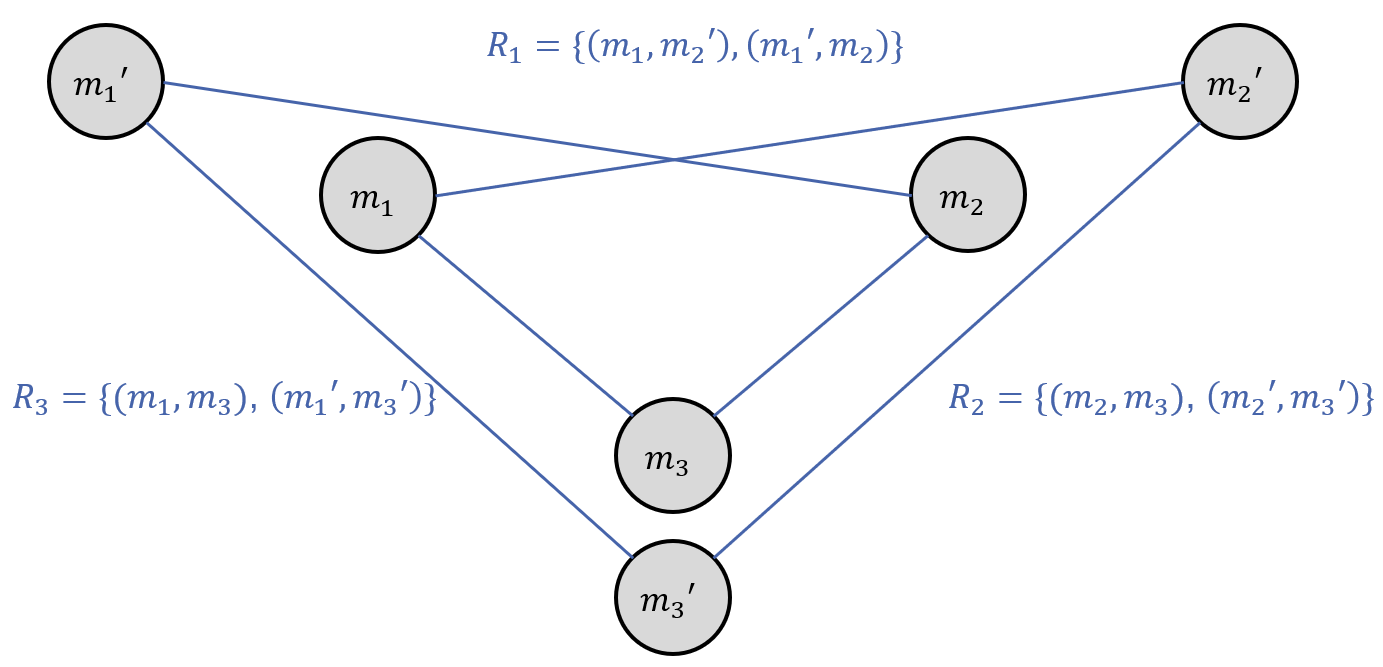
\includegraphics[width=\textwidth]{figures/correctness/compatibility/empty_global_relation.png}
    \caption[Consistency relations that imply an empty global relation]{Example for consistency relations that imply an empty global relation}
    \label{fig:compatibility:empty_global_relation}
\end{figure}

\mnote{Empty induced global relations indicate incompatibility}
In fact, if the relations induce an empty global relation, these relations do actually not properly fit to each other, because no single tuple of models would be considered consistent, thus no system could be consistently described.
We would thus consider such relations incompatible.
\autoref{fig:compatibility:empty_global_relation} shows an extended version of the example already given in \autoref{chap:correctness:notions_correctness:relations}, inducing an empty global relation.
This is an abstraction of the concrete examples, which we have already discussed for our our running example, in which modified consistency relations lead to an empty set of consistent model tuples, due to conflicting conversions and concatenations of names between persons, residents and employees.

\mnote{Goal of identifying incompatible relations}
There may, however, be more cases than empty induced global relations that we want to exclude by considering the relations incompatible.
In general, the goal of finding incompatibilities and excluding them is twofold:
First, we may want to identify that different developers of modular relations have an incompatible notion of consistent, such that the results would never be as expected.
This is what we have seen in the examples with the name relations.
We want to exclude these cases, because developers will not want to combine transformation based on relations that are contradicting.
Second, incompatibilities may lead to transformations not being able to find consistent models, so the orchestration would not be able to execute transformations in an order that achieves a consistent state.
If we, for example, encoded the relations from the running with the inverse concatenation of $firstname$ and $lastname$ ($R'_{PR}$) into transformations, each cycle in which the transformation are executed would produce one new person, employee, and resident, with swapped $firstname$ and $lastname$ and a comma appended to $lastname$.
In consequence, transformations would not be able to find a consistent state and, if not stopped preemptively, be executed endlessly.
Thus we also want to exclude such cases, because it can prevent a transformation network from termination.

%\begin{itemize}
    %\item We discussed that we are not interested in correctness of modular relations w.r.t. one monolithic relations, as that relations is usually unknown and thus correctness cannot be checked (cf ~\autoref{chap:correctness:notions:dimensions})
    %\item This would mean that modular relations are correct by construction
    %\item Although relations are, theoretically, correct by construction, we have seen that there are relations, for which we may say that they do not properly work together, i.e., they are \emph{incompatible}, as discussed in \autoref{chap:correctness:notions:relations}
    %\item There, we had three binary relations, which, taken together, do not impose an overall relation containing any consistent set of models, see \autoref{fig:compatibility:empty_global_relation}
    %\item We have already given a more concrete example for that case from our running example before.
    %\item It is obvious that we may not want to have an induced global relation that is empty, however, there may be more cases that we want to exclude.
    %%\item Exclude somehow defined \emph{incompatibilites} may be wanted for two reasons: First, we may want to identify that different developers of modular relations have an incompatible notion of consistency, such that the result would never be as expected (this is what we have seen for the names). Second, incompatibilites may lead to transformations not being able to find a consistent solution, so the orchestration would not be able to execute transformations to achieve a consistent state. To show that, we extend the relations example to a transformation example, showing that no consistent state can be reached, i.e., for an added person no consistent employees etc. can be found
%\end{itemize}


%%
%% OBSOLETE RELATIONS
%%
\subsection{Necessity of Obsolete Relation Elements}

\begin{figure}
    \centering
    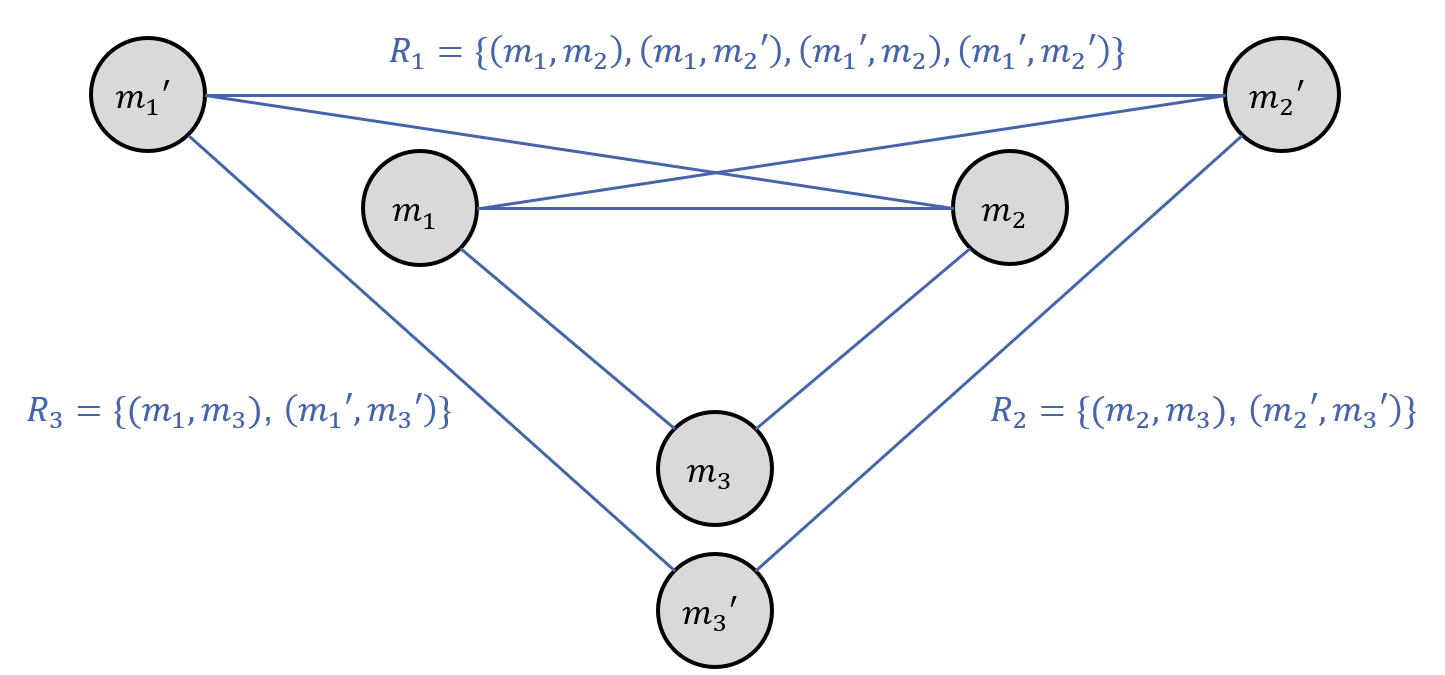
\includegraphics[width=\textwidth]{figures/correctness/compatibility/obsolete_relations.png}
    \caption[Example for obsolete elements in consistency relations]{Example for \enquote{obsolete} models pairs in consistency relation $R_1$, which can never occur in a globally consistent set of models}
    \label{fig:compatibility:obsolete_relations}
\end{figure}

\mnote{Locally consistent model pairs which are never globally consistent are \enquote{obsolete}}
A first intuitive option to define incompatibility is the presence of model pairs in the consistency relations, for which no globally consistent model tuple containing them can be found.
This canonically covers the case, in which the modular relations induce an empty global relation, because for none of the models pairs in each relation a globally consistent model tuple containing them can be found.
An example for that case is depicted in \autoref{fig:compatibility:obsolete_relations}, in which the relation $\consistencyrelation{R}{1}$ contains the pairs $\tupled{\model{m}{1}, \model{m}{2}'}$ and $\tupled{\model{m}{1}', \model{m}{2}}$, for which neither $\model{m}{3}$ nor $\model{m}{3}'$ is consistent to both other consistency relations, as the induced global relation is $\consistencyrelation{R}{} = \setted{\tupled{\model{m}{1},\model{m}{2},\model{m}{3}},\tupled{\model{m}{1}',\model{m}{2}',\model{m}{3}'}}$.
Thus, these model pairs may be denoted \enquote{obsolete} as they cannot occur in any globally consistent model tuple.

\mnote{Forbidding obsolete model pairs breaks assumptions}
While this point of view may be reasonable for the consistency relations only, as we are finally only interested in results that are globally consistent, it induces problems to the process of achieving such a result by means of transformation networks.
In fact, transformation networks need to allow intermediate states of models, which are only locally consistent, although they can never occur in a globally consistent state.
This is necessary, because otherwise each transformation would have to consider which model pairs are not only locally consistent but can be globally consistent as well.
We, however, excluded that by assumption of independent development and modular reuse and let the orchestration of transformations kind of negotiate a consistent result.

\begin{figure}
    \centering
    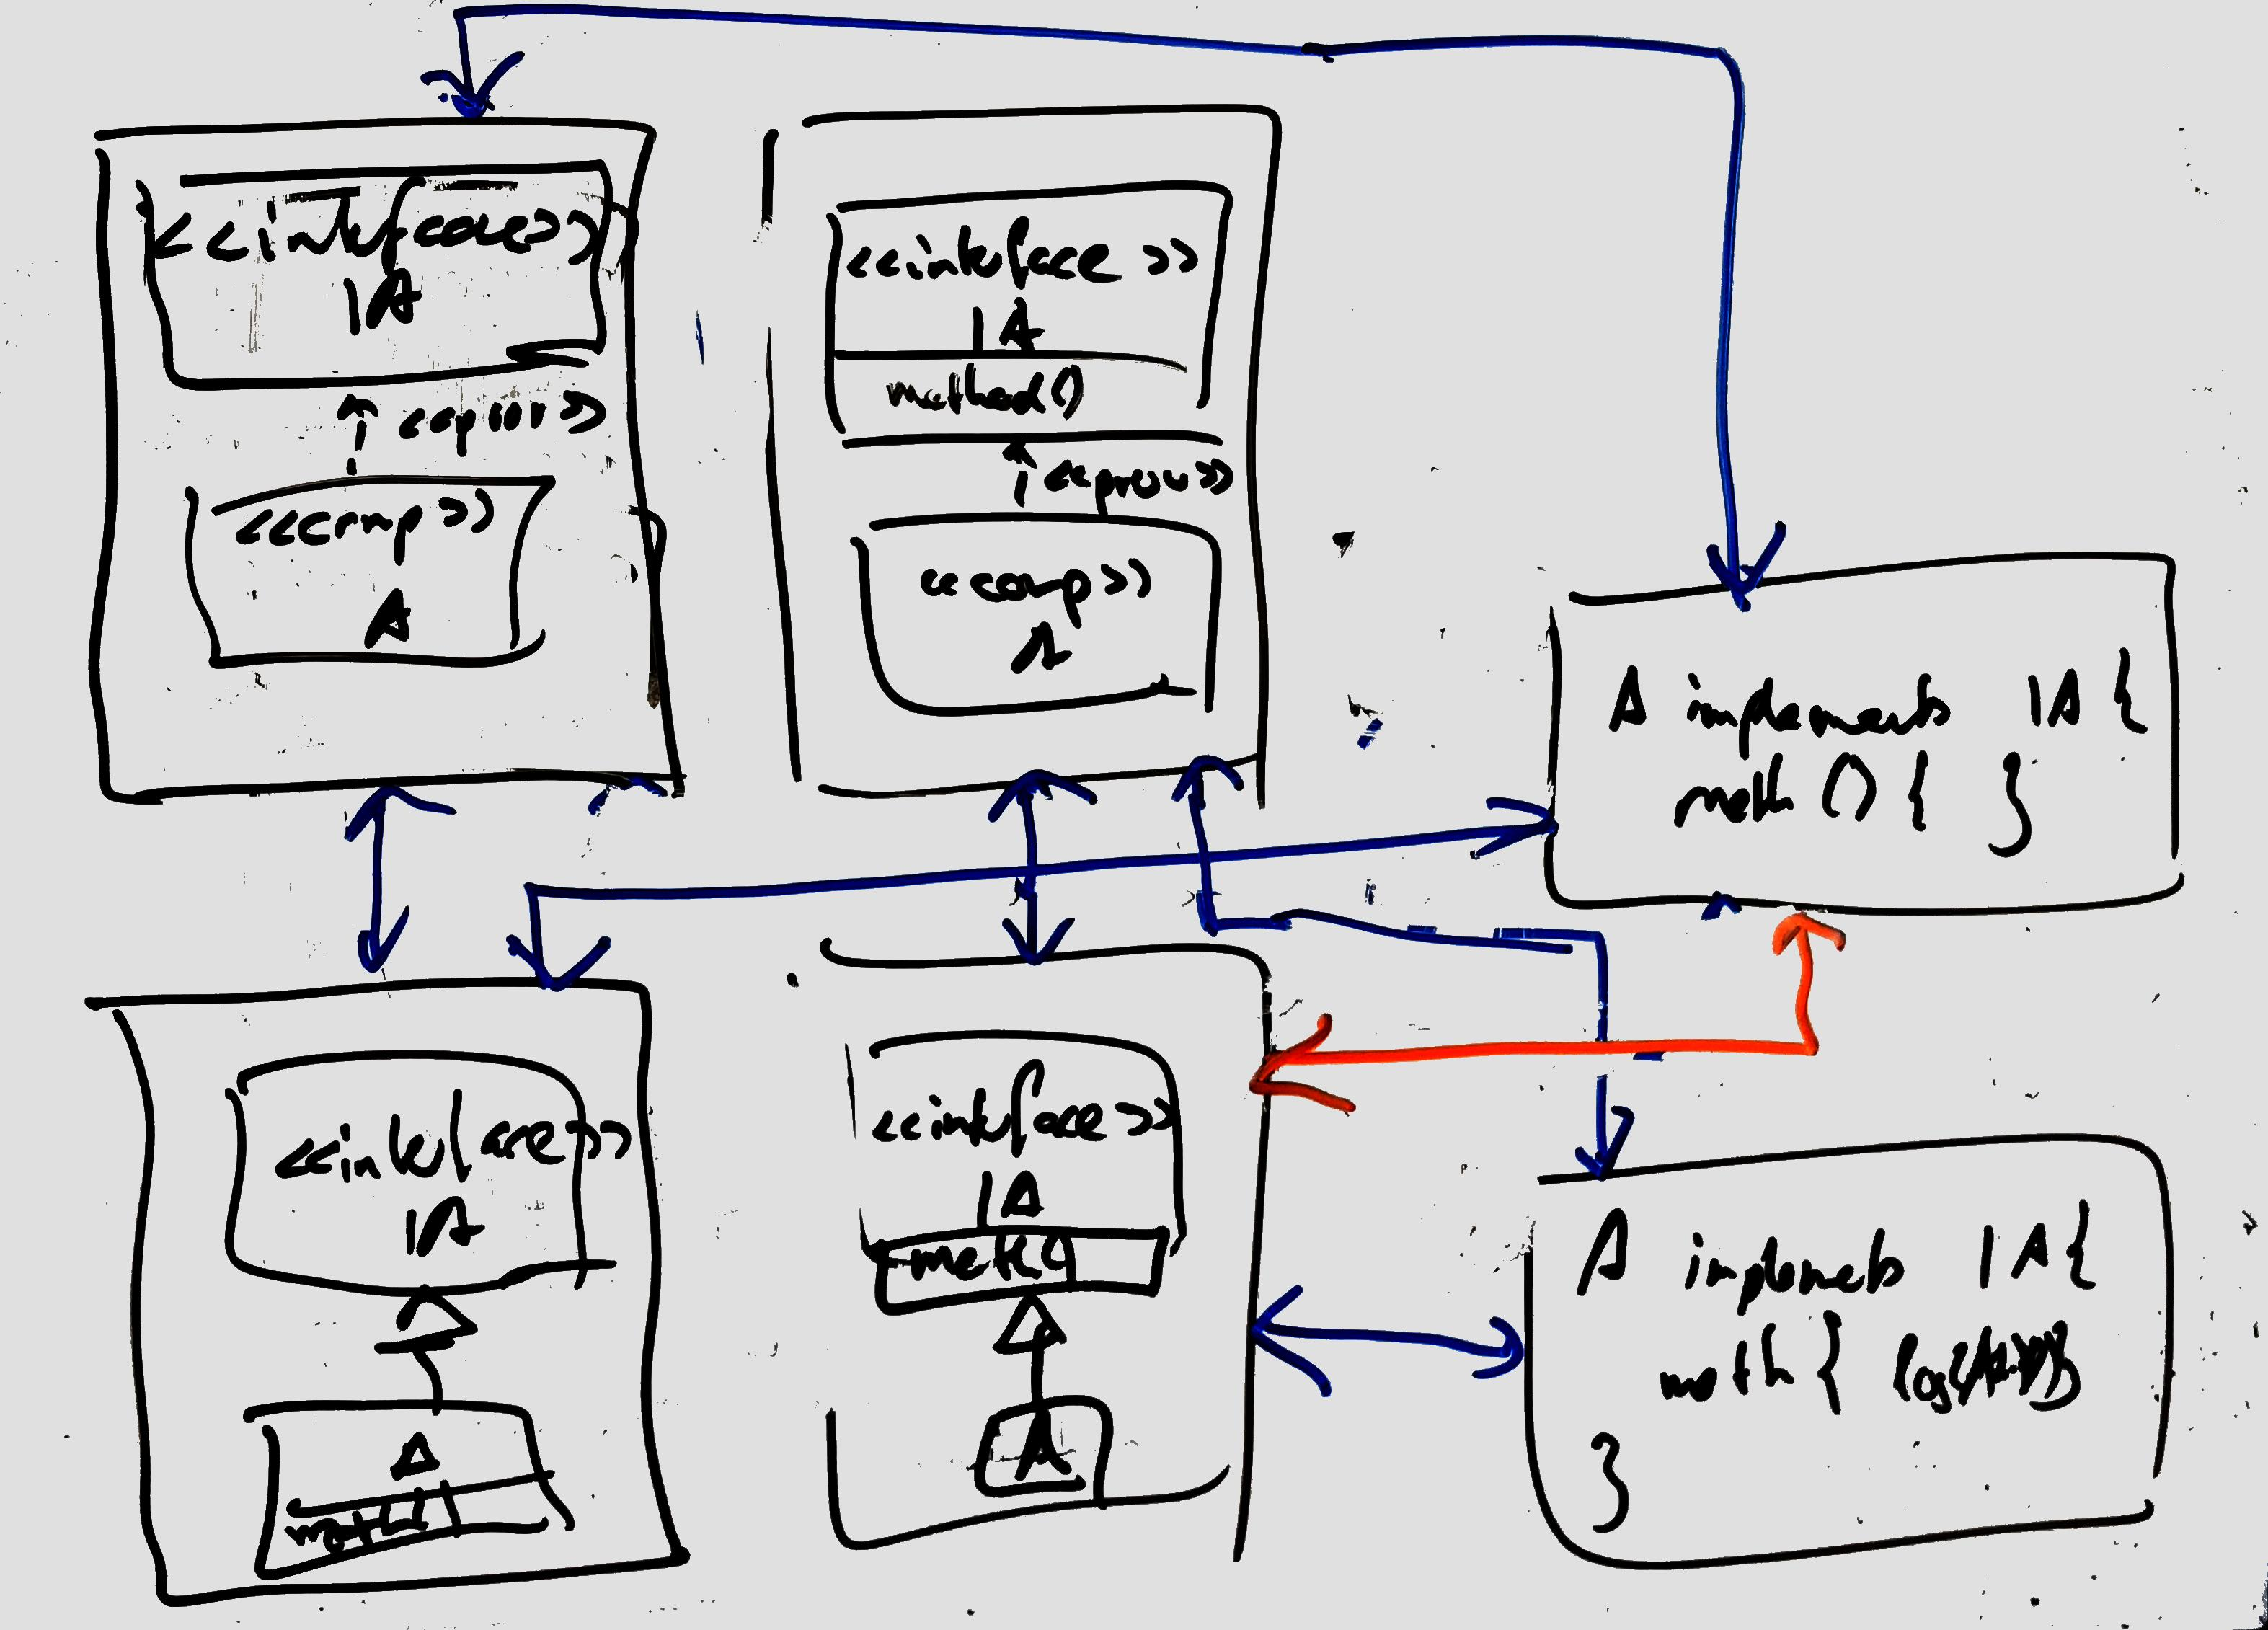
\includegraphics[width=\textwidth]{figures/correctness/compatibility/obsolete_relations_scenario.jpg}
    \caption[Concrete scenario with obsolete relation elements]{Example for an \enquote{obsolete} models pair in consistency relations between \gls{PCM}, UML and Java: The empty Java method realization cannot be globally consistent to the UML class model that defines the method in the class interface, because it realizes a \gls{PCM} component, for which the consistency relation requires at least a default implementation.}
    \label{fig:compatibility:obsolete_relations_scenario}
\end{figure}

\mnote{Example for obsolete relation necessity}
Consider the following example, which is also exemplarily depicted in \autoref{fig:compatibility:obsolete_relations_scenario}:
A UML class model and Java code are considered consistent when the same classes and interfaces with the same (in Java potentially empty) methods are contained.
In fact, for each UML model a usually infinite number of consistent Java models exists, containing arbitrary implementations of the methods.
In addition, \gls{PCM} models and UML class models are consistent when components are realized as classes implementing the provided interfaces of the components and thus their methods.
Analogously, each component is represented by a Java class implementing the provided interface.
The consistency relation between \gls{PCM} and Java may, however, require that a method within a class that realizes a method of a provided interface of a component has at least some default implementation, be it logging or something more component-specific.
%The transformation between \gls{UML} and Java may initialize a method added to a class with an empty body or dummy return statement.
%The transformation between \gls{PCM} and Java may, however, initializes a method within a class that realizes a component with a default implementation, be it logging or something more component-specific.
If we would now consider model pairs that can never occur in globally consistent model tuples as incompatible and thus forbid them, a UML model could not be considered consistent to a Java model if any method in a class that realizes a component and that is defined by one of its interfaces is realized by a Java method with an empty body.
The transformation between UML and Java would thus not be allowed to create an empty Java method upon creation of a UML method.
This would, however, enforce the relation between UML and Java to encode information about components, which both breaks our assumption of independent development, as the UML-Java transformation developer would need to know about that, and of modular reuse, because the transformation is then tied to the scenario in which \gls{PCM} is used as well.

\mnote{Obsolete relations do not induce a proper notion of incompatibility}
In consequence of the given scenario and the according insight that transformations may need to produce transient states that are only locally consistent to ensure independence of the transformations and their reusability in different contexts, such obsolete consistency relations do not induce a proper notion of incompatibility.

%First option: Remove "obsolete" relation elements

% \begin{itemize}
%     \item A first option might be to say that there should not be model pairs in the relations for which no globally consistent set of models can be found (give an abstract example for that)
%     \item However, in consequence a transformation could not produce such models, which might be necessary as transient (intermediate) states: E.g. a UML and Java code model are consistent when the same classes and interface with the same (in Java potentially empty) methods are present. In fact, a UML model is consistent with all (usually infinite) Java models with the same classes and methods, but with arbitrary method implementation. PCM and UML are consistent when components are realized as classes implementing the provided interfaces and thus their methods. Analogously, each component is represented by a Java class implementing the provided interfaces, but having an implementation that has some default functionality (be it logging or something more component-specific). 
%     Forbidding relations elements that can never be globally consistent would forbid that the relation between UML and Java allows Java models with empty method implementations for UML classes representing components. This would, however, require the relation/transformation between UML and Java know about components, which should not be the case due to modularity and independent development. Additionally, even in the concrete setup in which PCM is used, if a method is added to an interface of a class in UML which is a provided interface of its component in UML, the transformations may first create the Java method with an empty body, then propagate the method to the PCM interface and then propagate the default implementation of that method from PCM to Java. In this case, the transient state with the empty method body in Java is passed. Forbidding that would require an appropriate orchestration, i.e., first propagating the information across PCM, which could be defined for this specific case but not automatically decided in general, or the UML-Java transformation would have to consider that the Java implementation may not be empty, which, as discussed, contradicts modularity.
%     \item In general, this case is reflected in \autoref{fig:compatibility:obsolete_relations}, which shows two pairs in $R_1$, which can never occur in a globally consistent model, because the implied global relation is .... and does not contain those model pairs
% \end{itemize}


%%
%% UNWANTED BEHAVIOR
%%
\subsection{Prevention from Finding Consistent Solutions}
\label{chap:compatibility:informal:prevention}

% Second attempt: Derive incompatibility notion from unwanted behavior
\begin{figure}
    \centering
    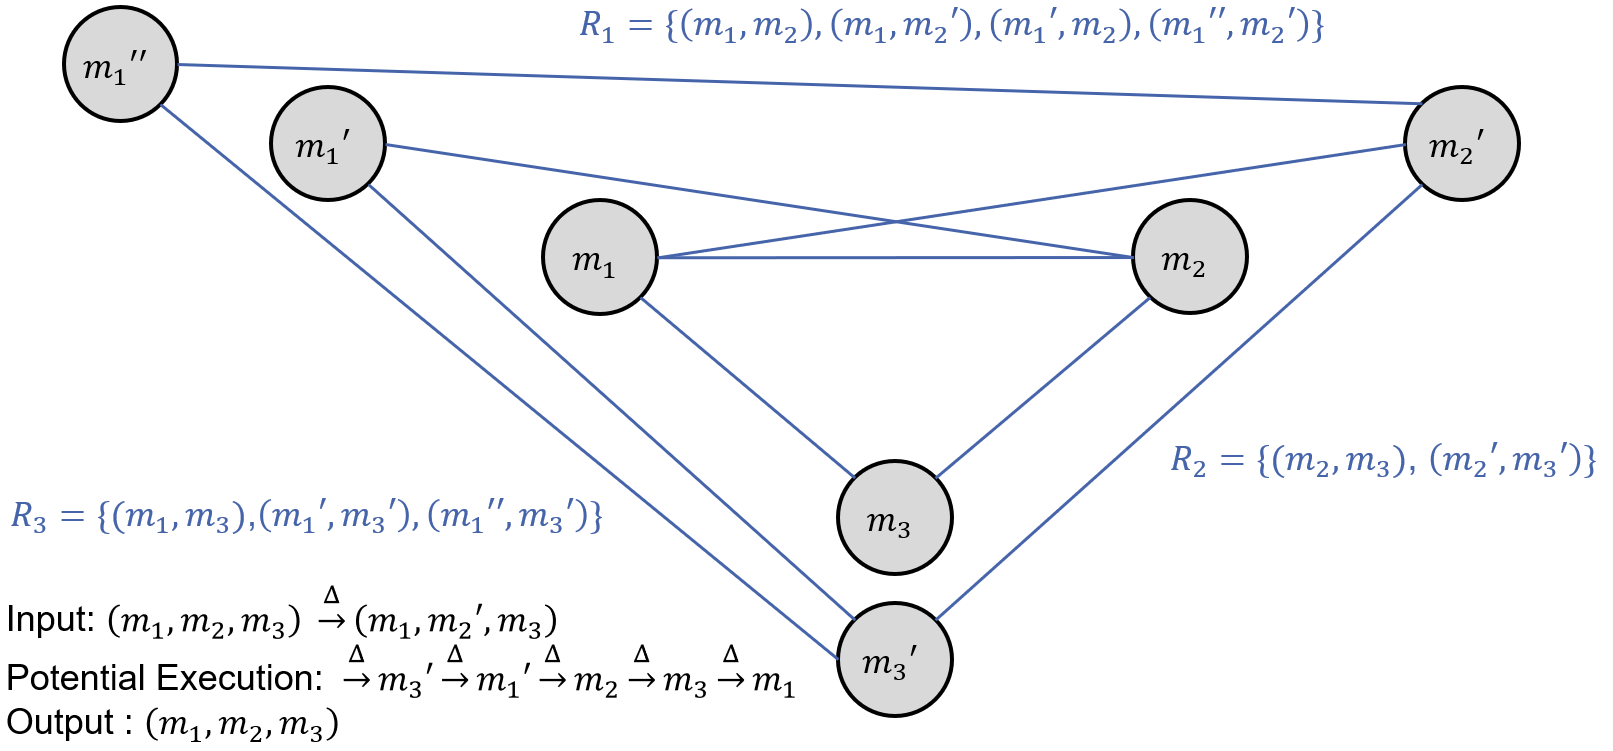
\includegraphics[width=\textwidth]{figures/correctness/compatibility/unwanted_behavior.png}
    \caption[Example for the unwanted rejection of a user change]{Example for the rejection of a user change because of consistency relations containing model pairs that are never globally consistent}
    \label{fig:compatibility:unwanted_behavior}
\end{figure}

\mnote{Example for transformation execution that reverts a user change}
To identify a proper notion of incompatibility, we now consider an exemplary transformation scenario from which we can derive such a notion.
In the example depicted in \autoref{fig:compatibility:unwanted_behavior}, we start with the models $\model{m}{1}$, $\model{m}{2}$ and $\model{m}{3}$, which are consistent to all three consistency relations.
If a user performs a change of $\model{m}{2}$ to $\model{m}{2}'$, we may assume the following transformation executions:
The transformation for $\consistencyrelation{R}{2}$ changes $\model{m}{3}$ to $\model{m}{3}'$, the one for $\consistencyrelation{R}{3}$ changes $\model{m}{1}$ to $\model{m}{1}'$ and then the one for $\consistencyrelation{R}{1}$ changes $\model{m}{2}'$ back to $\model{m}{2}$, as that is the only model consistent to $\model{m}{1}'$.
Now the transformation for $\consistencyrelation{R}{2}$ changes $\model{m}{3}'$ back to $\model{m}{3}$ and finally the one or $\consistencyrelation{R}{1}$ restores $\model{m}{1}$.
As a result, the transformation network executed the transformations in a way such that the original models are returned, which are actually consistent but reject the user change.

\mnote{Unnecessarily bad local selections can prevent network from finding proper solution}
Apart from the three given models, only $\model{m}{1}''$, $\model{m}{2}'$ and $\model{m}{3}'$ are consistent.
Upon the user change of $\model{m}{2}$ to $\model{m}{2}'$, we would actually expect the transformations to find the latter triple of models as a consistent result, as otherwise, like in the above example, the original models are returned, which actually rejects the user change.
The problem results from the model $\model{m}{1}'$ being present in the consistency relations, but not being consistent in any globally consistent model tuple.
For each of the transformations the local selection of $\model{m}{1}'$ is fine, as there are models to which it is locally consistent according to each consistency relation on its own.

\mnote{Scenario is different from obsolete relation elements}
Note that this scenario is different from the case discussed for obsolete relation elements.
In the scenarios discussed for obsolete relation elements, each model in such an obsolete pair occurs in a globally consistent model tuple, but not both models in that pair together do.
For example, the Java class with an empty method body actually occurs in a globally consistent model tuple, but not together with the UML class model in which the method is defined in the class interface, although they are locally consistent.

\mnote{Models that do not occur in any globally consistent model tuple are problematic}
We have seen that it is problematic, when consistency relations define consistency of models that do not occur in any globally consistent model tuple.
This can easily lead to transformations that do find the expected solutions and unnecessarily reject user changes.
We did not define a requirement that user changes may not be reverted on purpose, as that behavior may also be expected to express that certain changes are not allowed to be made.
However, if there was a reasonable series of transformations that returns a consistent tuple of models with reflects the user changes, it should be preferred over one that reverts the user change.

% \begin{itemize}
%     \item Considering the example in \autoref{fig:compatibility:unwanted_behavior}, we start with $A_1, B_1, C_1$ and have a user change of $B_1$ to $B_2$. Apart from the input models, only $A_3, B_2, C_2$ are globally consistent. So we would expect the transformations to find the latter models. Because of also having consistency relations to $A_2$ and transformation that locally select $A_2$ (because they do not know that there is no globally consistent state with $A_2$), passing across that model can lead to resulting in $A_1, B_1, C_1$ again. We did not define that requirement yet because it is not essentially necessary, but usually user may not want their changes be undone by a transformation, at least if there was another set of consistent models reflecting their change.
%     \item Thus, we would call this behavior unwanted.
%     \item Note that this scenario is different from the described scenario with empty Java method bodies, because in that case there are models for which an empty Java method body occurs in a globally consistent states (those in which the method does not realize a method of a provided interface of a component). Thus if the corresponding class does not realize a component but an ordinary class, it would be fine that it is consistent to the UML class with an empty body. In contrast, in the case described here, there is no single set of models in which $A_2$ was consistent.
% \end{itemize



%%
%% COMPATIBILITY NOTION
%%
\subsection{An Informal Notion of Compatibility}

\mnote{Models that are never globally consistent are problematic}
The discussed case that models do not occur in any globally consistent model tuple can be seen as a special case of obsolete relation elements, because it actually means that for each pair in a consistency relation in which a model occurs, the model pair cannot occur in a globally consistent model.
We found that in a combination of relations a model is problematic if
\begin{enumerate}
    \item it is locally consistent to another model, i.e., it occurs in a pair of a binary consistency relation and
    \item it can never be globally consistent, i.e., it is not contained in any model tuple that is consistent to all consistency relations.
\end{enumerate}
The model $\model{m}{1}'$ in \autoref{fig:compatibility:unwanted_behavior} was such a model, as it was locally consistent to $\model{m}{2}$ and $\model{m}{3}'$, but those two are inconsistent.

\mnote{Problematic models can be introduced by users or transformations}
We can distinguish two cases that lead to occurence of such a model like $\model{m}{1}'$:
\begin{properdescription}
    \item[User:] The model was created by the user, thus adapting the model is unwanted as the user introduced it. Such a change should be rejected as the model cannot be globally consistent.
    \item[Transformation:] The model was created by a transformation. In our example, this can either be the case because $\model{m}{2}$ or $\model{m}{3}'$ was created. There is, however, at least $\model{m}{1}''$ to which $\model{m}{2}$ and $\model{m}{3}'$ are consistent, so the transformation should better select that one. If there was not such $\model{m}{1}''$, then $\model{m}{2}$ and $\model{m}{3}'$ would be in the same situation not occurring in any globally consistent model tuple, thus the argumentation could be applied inductively.
\end{properdescription}
In consequence, allowing such models during the process of describing a system and preserving consistency between the system models does not provide any benefits and thus should in the best case not occur.
There is no reason to create it, but it may prevent transformations from finding consistent states.
In fact, disallowing the adaptation of the user change is even more reasonable when not concerning the complete model, like proposed with authoritative models by \textcite{stevens2020BidirectionalTransformationLarge-SoSym}, but only the part considered by a specific rule that describes consistency, such as a rule specifying the relation between classes and components, rather than between \gls{PCM} and UML.
This does also fit the way in which transformation are usually defined, as they consist of rules that relate only limited sets of meta-classes and their properties.
This is why our coming formalization of compatibility and its analysis will base on a more fine-grained notion of consistency, i.e., relations that relate extracts of models rather than the complete models.

\mnote{A notion of compatibility}
From these insights, we formulate the following, for now informal and still on the level of models, notion of compatibilility:
\begin{quote}
    For every model occurring in a pair of a consistency relation, a globally consistent model tuple containing it must exist.
\end{quote}

% 'This notion of compatibility reflects the intuitive requirements that we implicitly discussed.
% 'First, if the relation imply an empty global consistency relation, they are not considered compatible.
% Second, ...
% Informal notion reflects intuitive requirements:
% \begin{itemize}
%     \item We intuitively started to think about incompatibility in terms of relations implying an empty global relation. This is directly covered by the defined notion, because it that case for no single model a globally consistent tuple is found, thus the relations would be considered incompatible
%     \item We had the example of incompatible name mappings: Having a model with a single person, there is no globally consistent tuple of models, because the (faulty) inversion of firstname and lastname in one the relations leads to the necessity of having the person with inverted firstname and lastname in the model as well. This conflicts the introduced informal notion of compatibility.
%     As teasered before, we will precisely define the notion in a more fine-grained way at the level of elements rather than complete models. 
% \end{itemize}

\mnote{Compatibility notion is reasonable for preservation process}
This notion is especially reasonable when we consider the process of preserving consistency after user changes.
If a user performs a change, we want to ensure that if consistency of the modified elements is restricted by a consistency relation, there should be at least one consistent tuple of models that reflects the user change.
If this is not the case, the transformations will not be able to produce a reasonable result, apart from reverting or adapting the user change.

\mnote{Compatibility notion does not reflect specific semantic contradictions}
Note that this notion of compatibility does only exclude combinations of relations according to the above made argumentation of being generally useless and potentially preventing transformations from finding consistency result.
This does, however, not exclude further useless or unintended combinations of relations, for which the semantics of the relations would have to be known and analyzed.
The already discussed example of the necessity to infinitely swap $firstname$ and $lastname$ and append a comma induced by the alternative consistency relation $\consistencyrelation{R}{PR}'$ in \autoref{fig:compatibility:three_persons_example_extended} let to the situation that no tuple of models can fulfill those constraints, thus the global induced consistency relation is empty.
If we, however, relax $\consistencyrelation{R}{PR}'$ such that only $firstname$ and $lastname$ are swapped, but no comma is appended, the relations can be fulfilled by models which contain each person twice, once with its proper name and once with swapped first and last name.
Although we might say that the relations are not intended that way, it is impossible for a generic approach to validate that without knowing about the semantics of the attributes $firstname$, $lastname$ and their combination in $name$.
In a different context, it may be desired that two attributes are concatenated in both orders, thus it is generally necessary to not disallow that case.

\mnote{Compatibility is context-dependent and not achievable by construction}
Obviously, the given notion of compatibility is a property of a set of consistency relations and not of a single consistency relation on its own.
We may also say that compatibility of a single relation is \emph{context-dependent}.
In consequence, that property can neither be analyzed nor systematically achieved for a single consistency relation.
We can, by definition, not provide a construction approach for consistency relations to be compatible in each context.
Compatibility can only be achieved by construction if all consistency relations to be used together are known and developed together, such that compatibility can be analyzed on-the-fly.

%Derived (informal) notion of compatibility:
%\begin{itemize}
    % \item Models are problematic if
    % \begin{itemize}
    %     \item They can be locally consistent (according to one relation) to another model
    %     \item They are never globally consistent (not contained in any set of models that is consistent)
    % \end{itemize}
    % \item $A_2$ was such a model only being locally consistent with $B_1$ and $C_2$, but those are inconsistent.
    % \item Case Analysis:
    % \begin{itemize}
    %     \item $A_2$ is created by a user: Adapting this model is unwanted, as the user introduced it
    %     \item $A_2$ is created by a transformation: Either created because $B_1$ or $C_2$ was introduced. However, there are other $A_X$ to which $B_1$ and $C_2$ are consistent (otherwise they would be in the same situation as $A_2$), so the transformations should better select such a different $A_X$, as $A_2$ will never be consistent
    % \end{itemize}
    %\item As we can see from the example, considering such models does not provide any benefits (because they do never occur in a globally consistent state), but they can easily prevent transformations from finding a consistent state.
    %\item We can derive the following informal notion of incompatibility: For each model in a relation, a globally consistent model tuple must exist
    %\item More precisely, we will define this notion at the level of model elements rather than complete models, as transformations are usually defined in terms of rules that affect only some of the elements of models, such as a limited set of meta-classes and their properties.
%\end{itemize}


% Kompatibilität wird insbesondere interessant, wenn man annimmt, dass eine Nutzeränderung nicht rückgängig gemacht werden können soll. Wenn wir sie dann feingranular zerlegen, ist immer nur ein Element einer Relation betroffen, sodass dann relevant ist, ob wir hierfür Modelle finden könnten, die konsistent sind (wir diskutieren später bzgl. Orchestrierung, dass die Transformationen sie dann tatsächlich auch finden):
% Relationen müssen korrekt sein, d.h. gegeben eine Nutzeränderung muss es überhaupt möglich sein eine konsistente Menge an Modellen zu finden. Wenn Transformationen etwas beliebigen tun dürfen geht das immer. Wir nehmen an, dass eine Nutzeränderung nicht rückgängig gemacht werden soll (bzw. wenn sie rückgängig gemacht werden würde eigentlich die Änderung invalide war, d.h. keine Konsistenz im Netzwerk hergestellt werden kann). Daher sind Relationen nur korrekt, wenn für fixierte Elemente, die durch eine Nutzeränderung entstehen können, eine Modellmenge abgeleitet werden kann, die bzgl. der Relationen konsistent ist. D.h. gegeben einige Elemente muss es eine Modellmenge geben, die in allen Relationen liegt und die diese Elemente enthält (-> Kompatibilitätsbegriff). Wir betrachten in Kapitel ?, wie man Kompatibilität präzise definieren und feststellen/garantieren kann.\\
% Resultat: Gegeben eine Änderung ist es möglich eine Transformation anzugeben, die aus der Änderung ein konsistentes Modell produziert.

% \todo{In general, an empty set of consistent models can be intended. Without knowing about "semantics" it is impossible to validate whether restrictions are intended or not. However, we want to identify unintended situations, so we may define situations that we actually do not want to support, because there is a high possibility that the situation is unintended.}


\subsection{An Analysis for Compatibility of Relations}

\mnote{Overview of compatibility analysis approach}
In the following sections, we define a formal notion of compatibility and derive a formal, as well as practical approach for analyzing, or more precisely, proving it.
To give an overview of that approach, we first briefly introduce the central idea based on the given informal notion of compatibility, which we first introduced in \owncite{klare2018docsym} and \owncite{klare2019icmt}.

\mnote{Tree are compatible, but in general not achievable}
We have seen that incompatibilities can arise whenever there are cycles in the graph induced by consistency relations.
This means that the same models are related across two paths of relations, which may be contradictory.
Thus, to avoid incompatibilities by construction, one could define a network of transformations and thus underlying consistency relations that does not contain any cycles.
This situation is given when the network forms a tree.
As we have already discussed, it is, however, in general not possible to define such a tree.
First, it contradicts our assumption of independent development, as transformations would need to be aligned such that the missing direct relations between metamodels are expressed across other paths.
Second, like we have seen in the running example in \autoref{fig:compatibility:three_persons_example_extended}, if three metamodels all share specific information only pairwise, there needs to be a cycle of transformations to keep that information consistent.

\mnote{Redundancy and independence are compatibility-preserving}
Even if we cannot always construct tree, we can use the insight that trees of transformations consist of inherently compatible consistency relations to analyze arbitrary topologies for compatibility.
This is based on two techniques:
\begin{properdescription}
    \item[Redundancy:] If a consistency relation is redundant in a network, i.e., the same model tuples are considered consistent with or without that specific relation we can, virtually, remove it without affecting compatibility of the relations. More precisely, $\consistencyrelation{R}{1}$ is redundant in $\setted{\consistencyrelation{R}{1}, \consistencyrelation{R}{2}, \consistencyrelation{R}{3}}$ if and only if a model tuple $\tupled{\model{m}{1}, \model{m}{2}, \model{m}{3}}$ is consistent to $\setted{\consistencyrelation{R}{1}, \consistencyrelation{R}{2}, \consistencyrelation{R}{3}}$ exact when it is consistent to $\setted{\consistencyrelation{R}{2}, \consistencyrelation{R}{3}}$.
    Inductively applying the virtual removal of redundant relations until the remaining network is a tree, which is inherently compatible, we inductively know that the network with the redundant relations is compatible as well.
    \item[Independence:] When we consider consistency relations at the level of elements rather than models, the independence of relations is a second compatibility-preserving property.
    For example, if consistency between components and classes between \gls{PCM}, UML and Java is expressed in one set of relations and consistency between different interface representations in another, they can be considered independent, because modifications in components and classes do never affect interfaces and vice versa.
    Proving compatibility for each independent set of consistency relations inductively proves compatibility of the union of all these sets.
\end{properdescription}
Finding independent subsets of relations and removing their redundancies until only trees remain proves compatibility.
We call this approach \emph{decomposition}, as we decompose the original relations into independent, essential relations, and we say that the resulting trees \emph{witness} compatibility.

\begin{figure}
    \centering
    \input{figures/correctness/compatibility/independent_relations.tex}
    \caption[Exemplary overview of compatibility analysis idea]{Example for the decomposition of independent and removal of redundant consistency relations for analyzing compatibility. Adapted from \owncite{klare2018docsym}.}
    \label{fig:compatibility:decomposition}
\end{figure}

\mnote{Example for compatibility analysis}
Although we did not yet define how relations at the level of elements can be formally expressed, \autoref{fig:compatibility:decomposition} sketches the ideas for proving compatibility based on the given informal notion.
We have consistency relations $\consistencyrelation{R}{1}, \consistencyrelation{R}{2}, \consistencyrelation{R}{3}$ between three metamodels.
We know that $\consistencyrelation{R}{3}$ can be separated into disjoint $\consistencyrelation{R}{4}$ and $\consistencyrelation{R}{5}$, i.e., the relations are independent, thus one relation may related components and classes and the other may relate different interface representations, as exemplarily explained before.
Additionally, we know that the combination of $\consistencyrelation{R}{1}$ and $\consistencyrelation{R}{2}$ is a subset of $\consistencyrelation{R}{4}$, thus $\consistencyrelation{R}{4}$ is redundant as models are only considered consistent if they are consistent to $\consistencyrelation{R}{1}$ and $\consistencyrelation{R}{2}$ anyway.
In other words, $\consistencyrelation{R}{1}$ and $\consistencyrelation{R}{2}$ is more restrictive regarding consistency than $\consistencyrelation{R}{4}$.
In consequence, we can virtually remove $\consistencyrelation{R}{4}$ and consider $\consistencyrelation{R}{1}$ and $\consistencyrelation{R}{2}$ independently from $\consistencyrelation{R}{5}$, inductively due to its independence from $\consistencyrelation{R}{4}$.
The result are two independent trees of relations, which are inherently compatible.
Since redundancy and independence are compatibility-preserving, this proves that the original relations are compatible.

% \begin{copiedFrom}{ICMT}
% %FORMERLY: \subsection{Contradiction-free Modularizations}

% Contradictions in binary consistency specifications cannot be avoided by design.
% %They can, in the best case, be found by analyzing a combination of modular specifications.
% However, the structure of the network of specifications influences how prone to mistakes it is~\cite{klare2018docsym}.
% Two extremes of networks are depicted in \autoref{fig:correctness:modularization_strategies}:
% One is to have a specification for each pair of model types, inducing a dense graph. % of specifications.
% This extreme is prone to contradictions, because all relations are redundantly specified across several paths.
% Another extreme is to define each relation, potentially indirectly, only once, so that only one path of consistency specifications exists between each pair of model types.
% This leads to a tree of specifications, which is inherently free of contradictions and %, as there is only one path of specifications between each pair of model types.
% %Thus, it 
% avoids modularization mistakes by design.
% %Nevertheless, developers must understand the complete network to know which relations are represented, which is contradictory to our assumption of independent development.
% %Nevertheless, it breaks our assumption that specifications are developed independently, because relations are expressed indirectly, so developers must understand the complete network to know which relations are represented.
% However, it requires that such a network structure exists at all, because between three model types there must always be one relation that can be expressed transitively across the other two (cf.~\cite{klare2018docsym}).
% For example, if $\mathit{CS}_{1,3}$ in \autoref{fig:correctness:mistakes_specification_levels} shall be omitted and transitively expressed across $\mathit{CS}_{1,2}$ and $\mathit{CS}_{2,3}$, it must hold that:
% % \begin{align*}
% %     & \forall M_1 \in \mathcal{M}_1 : \forall M_2 \in \mathcal{M}_2 : \forall M_3 \in \mathcal{M}_3 : \\
% %     & \hspace{1em} \mathit{CS}(M_1, M_2, M_3) \iff \mathit{CS}_{1,2}(M_1, M_2) \land \mathit{CS}_{2,3}(M_2, M_3)
% % \end{align*}
% \begin{align*}
%     & \forall M_1, M_2, M_3 : (M_1, M_2, M_3) \in \mathit{CS} \Leftrightarrow (M_1, M_2) \in \mathit{CS}_{1,2} \land (M_2, M_3) \in \mathit{CS}_{2,3}
% \end{align*}
% %If this transitive relation misses or is even unable to express certain direct constraints, inconsistent models would be identified as consistent. %\todoHeiko{Das transitive muss man wohl an einem Beispiel erklären, am besten Ref. zu Intro}

% \begin{figure}[tb]
%     \centering
%     \input{figures/correctness/modularization_strategies.tex}
%     \caption{Extremes of Strategies for Modularizing Consistency Specifications}
% %    \todoHeiko{Ergänzen um Angaben Metamodelle und evtl. Relationsnamen. Angleichen zur Relationen-Grafik}
%     \label{fig:correctness:modularization_strategies}
% \end{figure}

% In consequence, if a network of transformation can be built that is a tree, mistakes at the modularization level are avoided by design.
% If a tree cannot be achieved, it is necessary to find and fix mistakes when transformations are combined to a network.
% In this case, the consistency specifications must be revised whenever non-termination or non-deterministic termination of consistency preservation is observed (see \autoref{fig:correctness:categorization}). %, or, if possible, analyzed for potential contradictions before execution~\cite{klare2018docsym}.
%This can potentially be supported by model checking techniques~\cite{klare2018docsym}.

% \subsection{Modularization Options}
% %ADD: We consider level 2 and 3, and assume level 1.
% %ADD: Transformations languages on level 2 or 3, but could also be on level 1
% \todoHeiko{ADD: Distinction on level 2 regarding one path / several paths -> redundancy or bottleneck -- Do that here?}
% \todoHeiko{Eigentlich brauchen wir der Argumentation nach diesen Abschnitt nicht. Er ist aber extrem wichtig. Irgendwo anders einbauen?}

% For modularizing consistency specifications, two extremes of approaches can be applied, as discussed in \cite{klare2018docsym} and depicted in \autoref{fig:modularization_strategies}. One of these extremes is to have each existing binary consistency relation represented in a consistency specification, which leads to a dense graph of specifications as shown in the left of \autoref{fig:modularization_strategies}. Another extreme is to define each consistency relation only across one path in the graph of consistency specifications, leading to a tree of consistency specifications as shown in the right of \autoref{fig:modularization_strategies}.

% \begin{figure}[tb]
%     \centering
%     \input{figures/modularization_strategies.tex}
%     \caption{Strategies for Modularizing Consistency Specifications}
%     \todoHeiko{Ergänzen um Angaben Metamodelle und evtl. Relationsnamen. Angleichen zur Relationen-Grafik}
%     \label{fig:modularization_strategies}
% \end{figure}

% To discuss the implications of the different strategies, we consider the simplified example in \autoref{fig:relations_example}. The relation $R$ is defined for three metamodels $\mathcal{M}_1, \mathcal{M}_2$ and $\mathcal{M}_3$ on system level (Level 1). This relation can be modularized into three binary relations $R_1, R_2 and R_3$ on modularization level (Level 2).

% \begin{figure}[tb]
%     \centering
%     \includegraphics[angle=270, width=0.7\textwidth]{figures/relations_example.pdf}
%     \caption{Example Relations on System and Modularization Level}
%     \label{fig:relations_example}
% \end{figure}

% The first extreme, to specify every existing consistency relation, has the advantage that modularity is very high in the sense that any subset of the metamodels between which consistency is specified can be selected and kept consistent when instantiating them. In the example, it is possible to use only instances of $\mathcal{M}_1$ and $\mathcal{M}_2$ for example, omitting $\mathcal{M}_3$ without losing the specification of certain consistency relations. 
% The drawback of this approach is the high degree of redundancy, as each consistency relations is specified multiple times across different paths. Those redundant specifications can easily contradict and lead to mistakes.
% The cause for contradicting consistency specifications is that at least one of them is not conform to the underlying consistency relation of the system. In the example, $R_1$ would be erroneous if the following condition holds:
% \begin{align*}
%     \exists M_1 \in \mathcal{M}_1 : \exists M_2 \in \mathcal{M}_2 : \exists M_3 \in \mathcal{M}_3 : [R(M_1, M_2, M_3) \land \neg R_1(M_1, M_2)] \lor [\neg R(M_1, M_2, M_3] \land R_1(M_1, M_2)]
% \end{align*}
% Since the relation $R$ is usually not specified explicitly, but implicitly through the partial, binary consistency specifications, such mistakes lead to contradictions between different binary consistency specifications.

% The second extreme, if each consistency relations is only represented across one path of consistency specifications, no redundancies exist, avoiding potential contradictions and mistakes induced by that. Nevertheless, it requires to find a network structure that is capable of representing all consistency relations without having multiple paths between two metamodels in the graph of consistency specifications. This requires that of three metamodels there is always one representing the overlapping information of the two others. 
% Therefore it must be possible to remove one of the relations without losing the representation of certain consistency relations. In the example, $R_3$ can be omitted, so that only $R_1$ and $R_2$ are used, if the following condition holds:
% \begin{align*}
%     \forall M_1 \in \mathcal{M}_1 : \forall M_2 \in \mathcal{M}_2 : \forall M_3 \in \mathcal{M}_3 : R(M_1, M_2, M_3) \Leftrightarrow R_1(M_1, M_2) \land R_2(M_2, M_3)
% \end{align*}
% If a developer accidentally leaves one a binary relation although the condition above is not fulfilled, some global consistency relations are not covered any more, which can lead to inconsistencies.

% An essential drawback of the second approach is that the network structure prescribes which parts of the consistency relations a binary consistency specification has to contain. Therefore, the consistency specifications cannot be developed independently, as their contents depend on those of the others. 
% \todoHeiko{Das letzte stimmt eigentlich nicht, denn auch bei dem anderen Verfahren muss man eigentlich die anderen Transformationen kennen, damit man Widersprüche vermeidet}
% \todoHeiko{Was wollen wir mit diesem Abschnitt jetzt eigentlich genau sagen?}

% \todoHeiko{MÖGLICHERWEISE: Diese Abschnitt hinter die Issues stellen als Begründung für die Issues und deren Diskussion auf Level 2? Dann steht das ungefähr auf einer Ebene mit Level 3! Könnte man auch in eigenes Kapitel packen, dann werden Level 2 und Level 3 explizit behandelt, Level 1 schließen wir ja eh aus. Gefällt mir auf den ersten Blick VIEL BESSER.}

% \end{copiedFrom} % ICMT


% \begin{copiedFrom}{DocSym}

% Defining a tree of transformations to preserve consistency between multiple models is difficult, because of three metamodels there must always be one containing all overlapping information of the two others.
% It is easy to see that this is hardly applicable in practice.
% %Even if all metamodels basically have a refinement relation, there may be some additional information in more abstract metamodels not represented in the more fine-grained ones.
% Nevertheless, it may be sufficient to find subsets of independent consistency relations, of which each induces such a tree, instead of considering the whole set of relations between two metamodels.
% %For example, defining the consistency relations between \ac{ADL} components and classes and those between service functionality specifications in an \ac{ADL} and class methods may require a fully connected graph of consistency relations between \ac{ADL}, \ac{UML} and Java, but treating them independent of each other, each of them may be representable by a tree of relations.
% For example, consider the relations in \autoref{fig:correctness:decomposition}.
% \ref{fig:correctness:independent_relations:R3} represents a subset of the transitive relation $\mbox{\ref{fig:correctness:independent_relations:R1}} \concat \mbox{\ref{fig:correctness:independent_relations:R2}}$.
% In consequence, \ref{fig:correctness:independent_relations:R3} can be omitted, but the remaining consistency relations still form a graph.
% However, since \ref{fig:correctness:independent_relations:R4} is independent from the other relations, it can be treated separately from the others, resulting in two trees of independent consistency relations.

% \begin{figure}
%     \centering
%     \input{figures/correctness/independent_relations.tex}
%     \caption{Exemplary decomposition of consistency relations}
%     \label{fig:correctness:decomposition}
% \end{figure}

% In our thesis, we will therefore analyze different case studies for the existence of such independent consistency relations, which allows to decompose them to independent trees.
% We will develop an appropriate representation of consistency relations, which is more sophisticated than the set notation used in this paper, and an analysis for independence of those relations.
% We will then investigate how that can be integrated into existing, declarative transformation languages.
% In consequence of that, we improve the \emph{applicability} of a tree-based specification of transformations.

% \todo{Hier fehlt noch was}
% %The notion of such relations to be sets of element tuples that is used here here is only used for illustration, as is hard to reduce actual relations of \metaclasses and their elements to such tuple sets.
% \todo{Erik: Ich finde, daß bis hier im Text noch zu wenig klar wird, daß es hier um Konsistenzrelationen geht. Man könnte auch den Eindruck bekommen, es geht generell um Transformations-Strukturen, die z.B. weder bidirektional noch inkrementell sein müssen. Natürlich haben wir auch wieder das Grundproblem, daß wir \emph{Konsistenz} nicht sauber definiert haben, aber das Faß will man hier vielleicht nicht aufmachen \ldots}

% \end{copiedFrom} % DocSym


\section{A Formal Notion of Compatibility}
\label{chap:compatibility:formal_notion}

%\begin{copiedFrom}{SoSym MPM4CPS}

\mnote{Formal notion of fine-grained consistency and compatibility}
In this section, we precisely define our, yet informally introduced notion of \emph{compatibility}.
%We first discuss properties of transformation networks %in comparison to a single transformation 
%with an intuitive notion of compatibility, based on considerations in existing work.
For that, we use the fine-grained notion of consistency and defining relations as proposed in \autoref{chap:correctness:finegrained}.
We discuss implicit relations, which are induced by a set of consistency relations, such as transitive relations, and,
finally, derive a compatibility notion from the consistency formalization and its pursued perception.
%To distinguish the previously given coarse-grained and the coming fine-grained definition of consistency and consistency relations, we used the \enquote{model-level} prefix in the coarse-grained notion.
The contents of this and the remaining sections of this chapter are mostly, even literally, taken from our published article on proving compatibility~\owncite{klare2020compatibility-report}.

%This serves as our contribution \ref{contrib:formalization}.
%An introduction to properties of transformation networks and especially compatibility of transformations, what compatibility means and how the network influences the possibility to give guarantees regarding compatibility.

%\todoHeiko{Discuss extensional definition of relations / constraints and its relation to intensional definitions}
% \subsection{Properties of Transformation Network}
% \label{sec:compatibility:networkproperties}

% %% Correctness as a property of single, bidirectional transformations
% Keeping pairs of models consistent by means of incremental, bidirectional transformations has been well researched in recent years~\cite{stevens2010sosym, etzlstorfer2013a, cleve2019dagstuhl}.
% A bidirectional transformation consists of a \emph{relation} that specifies which pairs of models are considered consistent and a pair of directional transformations, denoted as \emph{consistency repair routines}, that take one modified and one originally consistent model and deliver a new model that is consistent to the modified one~\cite{stevens2010sosym}.
% Several well-defined properties of such transformations have been identified.
% The essential \emph{correctness} property states that a consistency repair routine delivers a result such that the models are actually consistent according to the defined relation~\cite{stevens2010sosym}.
% Another important property is \emph{hippocraticness}, which states that a consistency repair routine returns the input model if it was already consistent to the modified one~\cite{stevens2010sosym}.

%%
%% Correctness property of transformation networks, not induced by correctness of single transformations
%%
% When we combine several transformations to a network to achieve consistency between multiple models, those properties of the single transformations are still relevant, as each transformations on its own has to be at least correct to work properly in a network of transformations.
% However, correctness of the single transformations does not induce correctness of the transformation network.
% Taking an arbitrary set of correct transformations and executing them one after another does not necessarily constitute a terminating approach that delivers a result, in which all models are consistent according to the relations of the transformations, because the result of one transformation may violate the relation of another.
% It is possible that the approach does either not terminate, because there is a divergence or alternation in values changed or elements created, or terminates in a state that is not consistent regarding the relations of all transformations~\cite{klare2019icmt}.
% %Consider the example of $R_{PE}, R_{PR}, R'_{ER}$ in \autoref{fig:motivational_example}. A transformation network in which each transformation adds the corresponding element for an added element, such as a resident for an added person by the transformation of $R_{PR}$.
% \todoDiss{Readd}
% %Since the execution of one transformation may lead to a violation of the relation of another transformation, executing each transformation only once can easily lead to termination in an inconsistent state.
% %In consequence, transformations have to be executed in a fixed point iteration manner, until all relations are fulfilled.
% The property of a network to always result in a state in which the models are consistent to all relations of the transformations if they are executed in a specific order, can be seen as a \emph{correctness} property for transformation networks.
% In this work, we focus on that correctness property and do not discuss further quality properties of transformation networks, such as \emph{modularity}, \emph{evolvability} and \emph{comprehensibility}~\cite{klare2018docsym}.


%%
%% Correctness considerable at different levels.
%%
% A single transformation can only be incorrect in terms of its repair routines, because there are no restrictions regarding its relation that may prevent the repair routine from being able to produce a correct result.
% In previous work, however, we identified that transformation networks can be incorrect at different levels~\cite{klare2019icmt}.
% Networks can also be incorrect at the level of relations rather than repair routines, because multiple relations can be contradictory, i.e., they can relate elements in different ways such that the relations cannot be fulfilled at the same time.
% \todoDiss{Readd}
%This especially concerns the \emph{modularization level}, which considers correctness of the binary relations of a set of bidirectional transformations describing when a set of models is consistent, and the \emph{operationalization level}, which considers correctness of the consistency repair routines in terms of producing models that are correct regarding the relations of all bidirectional transformations.
%For a single transformation, there are no restrictions regarding its relation that may prevent the repair routines from being able to produce a correct result, thus correctness is only considered at the operationalization level. %The correctness definition of \textcite{stevens2010sosym} for a single transformation only concerns the operationalization level, because a single relation is correct by construction. 
% Considering only a single transformation, its relation is correct by definition, at least if there is no external specification against which the relations have to be correct, thus the definition of \textcite{stevens2010sosym} for correctness only considers the consistency repair routines.
%However, in case of a transformation network, the different relations may be contradictory, i.e., elements are related in a different way such that the relations cannot be fulfilled at the same time.
% In such a case, the consistency repair routines cannot be result in a state that is consistent according to the relations anymore, thus they may not terminate anymore.
%This is due to the fact that several relations can relate the same elements in a different way, such that they cannot be fulfilled at the same time, i.e. that they are contradictory.
%In such a case, the iteration will not terminate.
% We call the relations of such transformations \emph{incompatible}.
%We define this informal notion of compatibility more precisely in the remainder of this section.

%%
%% Compatibility not achievable by construction -> we focus on checking it
%%
% In consequence, compatibility of relations is a necessary prerequisite for consistency repair routines to produce correct results in transformation networks.
% We also found that correctness of the consistency repair routines can already be achieved by construction, whereas compatibility of the relations cannot be achieved by construction but in the best case be checked for a set of relations.
% In this work, we focus on the possibility to check compatibility of the relations of a set of transformations.
% In the following, we therefore precisely define the notion of compatibility of relations, which excludes contradictions in relations that can prevent consistency repair routines from fulfilling the relation.

% \todo{Example!}

%%
%% Tree topology excludes compatibility
%%
%\subsection{Network Topology Impacts}
% Finally, the topology of a transformation network directly influences how prone it is to incompatibilities of its relations.
% Contradictions of consistency relations, as exemplified with the relations $R_{PE}, R_{PR}, R'_{ER}$ in \autoref{fig:prologue:three_persons_example}, can only occur if the same classes are related to each other by different (sequences of) transformations in a different way.
% For example, in \autoref{fig:prologue:three_persons_example}, each combination of two relations puts the same classes into relation as the third one.
%This can also be a the case if a sequence of transformations introduces this relation, like each combination of two relations in \autoref{fig:motivational_example} relates the same classes as the third relation.
% This means that a transformation network, in which each pair of classes is only related by one sequence of transformations, cannot have contradictory relations and is thus inherently compatible.



% \subsection{Consistency by Transformation Networks}

% \begin{itemize}
%     \item Incremental, bidirectional transformations serve as a means for preserving consistency of models by updating one if the other is modified
%     \item Transformations specify the conditions for consistency (consistency relations), as well as how consistency can be restored after modifications (consistency repair)~\cite{stevens2010sosym}
%     \item Consistency between more than two models can be achieved by coupling bidirectional transformations to networks
%     \item Even if the single transformations are correct, i.e. consistency repair produces results that conform to the consistency relations~\cite{stevens2010sosym}, this may not be the case when \emph{independently developed} bidirectional transformations are combined.
%     \item Interoperability problems can occur at the level of consistency relations, i.e. that the relations of the different transformations cannot be fulfilled at the same time, or at the level of consistency repair, i.e. that the repair routines do not terminate in a consistent state or even not at all~\cite{klare2019icmt}
%     \item While \textcite{klare2019icmt} focused on techniques to avoid interoperability issues at the level of consistency repair, in this work we focus on finding interoperability issues of the underlying consistency relations, which we previously defined as \emph{compatibility} issues~\cite{klare2018docsym}.
%     The avoidance of interoperability issues at the relations level is a necessary assumption to avoid issues at the operationalization level.
% \end{itemize}


% \subsection{Network Topology Impacts}

% \begin{itemize}
%     \item Idea: Couple independently developed transformations (refer to running example) to network
%     \item Problem: Trade-off between different properties, depending on the chosen or induced network topology
%     \item Introduce contrary properties \emph{compatibility} and \emph{modularity} (provide only a naive explanation) and shortly refer to evolvability/comprehensibility \cite{klare2018docsym}.
%     \item Explain problems of building tree structures (inherent compatibility) and motivate arbitrary graph structures, providing high modularity, but not giving compatibility guarantees
% \end{itemize}

%\end{copiedFrom} % SoSym MPM4CPS

%%%%%%% MOVED FINE-GRAINED RELATION INTRODUCTION TO CORRECTNESS CHAPTER


\begin{copiedFrom}{SoSym MPM4CPS}

\subsection{Implicit Consistency Relations}

Considering sets of consistency relations, as they are implicitly defined by the set of transformations in a transformation network, their combination is of especial interest.
Each set of consistency relations defines relations between two sets of classes.
However, such consistency relations imply further \emph{transitive} consistency relations.
Having one relation between classes $A$ and $B$ and one between $B$ and $C$ implies an additional relation between $A$ and $C$, for which we define a notion for the concatenation of relations.
The goal of this notion is to provide a relation that is induced by the concatenated ones. This means, if a model is consistent to the concatenation, it should also be consistent to the single relations, as otherwise the concatenation would introduce additional consistency constraints.
To achieve this, the following definition makes appropriate restrictions to the derived consistency relation pairs.

\todo{Actually, a concatenation may also consider that two or more relations are concatenated to a single one. I.e. CR1 could map something to A and B, and CR2 could map A to something and CR3 could map B to something. Then there could be a combination of all of them. In fact, each pair of consistency relations between the same metamodels can be combined to "larger" relation that then may be concatenated to other relations. Such a pair could even be a pair of a relation with itself, like if a relation maps on element to two of the same class and another relation then maps one element of the class to another. 
In summary, our notion of transitivity has to consider that concatenation may not only be sequences, but acyclic graphs.}

\begin{definition}[Consistency Relations Concatenation] \label{def:relationconcatenation}
    Let $\consistencyrelation{CR}{1}, \consistencyrelation{CR}{2}$ be two consistency relations. The concatenation is defined as follows:
    \begin{align*}
        &
        %\consistencyrelation{CR}{} = 
        \consistencyrelation{CR}{1} \concat \consistencyrelation{CR}{2} := \setted{\tupled{\conditionelement{c}{l}, \conditionelement{c}{r}} \mid \\
        & \formulaskip 
        \exists %\consistencyrelationpair{cr}{1} = 
        \tupled{\conditionelement{c}{l}, \conditionelement{c}{r,1}} \in \consistencyrelation{CR}{1} : \exists %\consistencyrelationpair{cr}{2} = 
        \tupled{\conditionelement{c}{l,2}, \conditionelement{c}{r}} \in \consistencyrelation{CR}{2} : %\conditionelement{c}{l,1} = \conditionelement{c}{l} \land \conditionelement{c}{r,2} = \conditionelement{c}{r} \\
        %& \formulaskip\formulaskip
        %\land 
        \conditionelement{c}{r,1} \subseteq \conditionelement{c}{l,2}\\
        & \formulaskip
        \land \forall \tupled{\conditionelement{c}{l}, \conditionelement{c'}{r,1}} \in \consistencyrelation{CR}{1} : \exists \tupled{\conditionelement{c'}{l,2}, \conditionelement{c'}{r,2}} \in \consistencyrelation{CR}{2} : \conditionelement{c'}{l,2} \subseteq \conditionelement{c'}{r,1}
        }
    \end{align*}
    with $\classtuple{C}{l,\consistencyrelation{CR}{}} = \classtuple{C}{l,\consistencyrelation{CR}{1}}$ and $\classtuple{C}{r,\consistencyrelation{CR}{}} = \classtuple{C}{r,\consistencyrelation{CR}{2}}$
\end{definition}

The concatenation of two consistency relations contains all pairs of object tuples that are related across common elements in the right respectively left side of the consistency relation pairs.
Such a concatenation may be empty.
Two requirements ensure that all models considered consistent to the concatenated relation are also consistent to the single relations:
First, it is important that a pair of consistency relations $\consistencyrelation{CR}{1}, \consistencyrelation{CR}{2}$ is only combined if the left condition element of the consistency relation pair from $\consistencyrelation{CR}{2}$ is a subset of the right condition element of the consistency relation pair $\tupled{\conditionelement{c}{l}, \conditionelement{c}{r}}$ of $\consistencyrelation{CR}{1}$.
%For example, if $\consistencyrelation{CR}{1}$ requires for an element $a$ the elements $b$ and $c$ to exist, then $\consistencyrelation{CR}{2}$ must define a relation for a subset of $b$ and $c$, such that it transitively requires the existence of further elements.
Second, it is necessary that for all elements $\conditionelement{c}{r}$ in the right side of $\consistencyrelation{CR}{1}$, to which a condition element $\conditionelement{c}{l}$ is considered consistent, there must be a matching condition element, i.e. a subset of $\conditionelement{c}{r}$, in the left condition of $\consistencyrelation{CR}{2}$.
Otherwise, in both cases the occurrence of $\conditionelement{c}{l}$ in a model tuple would not necessarily impose any consistency requirement by $\consistencyrelation{CR}{2}$.
In the following, we explain these two requirements at an example.

% \begin{figure}
%     \centering
%     \includegraphics[width=\columnwidth]{figures/concatenation_subset.png}
%     \caption{Two consistency relations with $\consistencyrelation{CR}{1} \concat \consistencyrelation{CR}{2} = \emptyset$ and $\consistencyrelation{CR^T}{2} \concat \consistencyrelation{CR^T}{1} \neq \emptyset$}
%     \label{fig:concatenation_subset}
% \end{figure}

% \begin{figure}
%     \centering
%     \includegraphics[width=\columnwidth]{figures/combined_concatenation_example.png}    \caption{Consistency relations $\consistencyrelation{CR}{1}$ and options $\consistencyrelation{CR}{2}, \consistencyrelation{CR'}{2}, \consistencyrelation{CR''}{2}$ with $\consistencyrelation{CR}{1} \concat \consistencyrelation{CR}{2} = \neq \emptyset$, $\consistencyrelation{CR}{1} \concat \consistencyrelation{CR'}{2} = \emptyset$, $\consistencyrelation{CR}{1} \concat \consistencyrelation{CR''}{2} = \emptyset$ and $\consistencyrelation{CR''^T}{2} \concat \consistencyrelation{CR^T}{1} \neq \emptyset$}
%     \label{fig:concatenation_example}
% \end{figure}


\begin{figure}
    \centering
    \begin{subfigure}{\textwidth}
        \centering
        \input{figures/correctness/compatibility/concatenation_example}
    \end{subfigure}

    \vspace{1em}
    \begin{subfigure}{\textwidth}
        \centering
        \input{figures/correctness/compatibility/concatenation_subset_example}
    \end{subfigure}
%    \includegraphics[width=\columnwidth]{figures/consistency_concatenation_example.png} 
    %\includegraphics[width=\columnwidth]{figures/concatenation_subset.png}
    \caption[Examples for consistency relation concatenation]{Two scenarios, each with two consistency relations: 
    Consistency relations $\consistencyrelation{CR}{1}$ and two options $\consistencyrelation{CR}{2}, \consistencyrelation{CR'}{2}$ with $\consistencyrelation{CR}{1} \concat \consistencyrelation{CR}{2} \neq \emptyset$ and $\consistencyrelation{CR}{1} \concat \consistencyrelation{CR'}{2} = \emptyset$, and consistency relations $\consistencyrelation{CR}{3}$ and $\consistencyrelation{CR}{4}$ with $\consistencyrelation{CR}{3} \concat \consistencyrelation{CR}{4} = \emptyset$ and $\consistencyrelation{CR^T}{4} \concat \consistencyrelation{CR^T}{3} \neq \emptyset$. Taken from \owncite{klare2020compatibility-report}.}
    \label{fig:compatibility:concatenation_example}
\end{figure}

\begin{example}
\autoref{fig:compatibility:concatenation_example} extends the initial example (\autoref{fig:compatibility:three_persons_example_extended}) with further classes in the consistency relations, such that they do not only relate single classes to each other.
It defines an address for employees and in the second example also a location for the address of residents, which are represented in additional classes.
Both examples contains a consistency relation $\consistencyrelation{CR}{1}$ respectively $\consistencyrelation{CR}{3}$ between persons and residents, which define that for each person a resident with the same name has to exist.
The examples provide different options for consistency relation between residents (with locations) and employees with addresses ($\consistencyrelation{CR}{2}, \consistencyrelation{CR'}{2}, \consistencyrelation{CR}{4}$), which exemplify the necessity for the restrictions in \autoref{def:relationconcatenation}:
\begin{enumerate}
    \item $\consistencyrelation{CR}{1} \concat \consistencyrelation{CR}{2}$: 
$\consistencyrelation{CR}{2}$ requires for each resident an employee with the same name and an address with an arbitrary street name.
In consequence, $\consistencyrelation{CR}{1} \concat \consistencyrelation{CR}{2}$ defines a relation for each person with an employee having the same name and all addresses with possible street names.
All models that are consistent to the concatenation are also consistent to the single relations.
    \item $\consistencyrelation{CR}{1} \concat \consistencyrelation{CR'}{2}$: 
$\consistencyrelation{CR'}{2}$ is similar to $\consistencyrelation{CR}{2}$ but additionally requires that the street of a resident must not be empty. 
In consequence, for a resident with an empty address it is not required that an employee exists.
This results in $\consistencyrelation{CR}{1} \concat \consistencyrelation{CR'}{2} = \emptyset$, because for any person, there must not be an employee, as the person can be consistent to a resident with an empty street name.
This shows the necessity of the second restriction in the definition. 
    \item $\consistencyrelation{CR}{3} \concat \consistencyrelation{CR}{4}$: 
The concatenation $\consistencyrelation{CR}{3} \concat \consistencyrelation{CR}{4}$ is obviously empty, because $\consistencyrelation{CR}{3}$ requires a resident for each person, but $\consistencyrelation{CR}{4}$ only requires an employee if there is also a location.
Such a location does not necessarily exist if a person %and thus a resident
exists, thus if the models are consistent to $\consistencyrelation{CR}{3}$ and $\consistencyrelation{CR}{4}$ there must not necessarily be an employee for any contained person.
This shows the necessity for the first restriction in \autoref{def:relationconcatenation}, which would require a left condition element from $\consistencyrelation{CR}{4}$ (resident and location) to be a subset of a right condition element in $\consistencyrelation{CR}{3}$ (resident). %, which is never the case. % because of $\consistencyrelation{CR}{4}$ requiring more elements than $\consistencyrelation{CR}{3}$ ensures to exist or a person.
%This shows the necessity of the first restriction in the definition, which requires for all persons that for each consistent resident according to $\consistencyrelation{CR}{3}$, there is also a condition in $\consistencyrelation{CR}{4}$ that requires an employee to exist.
%However, generally speaking, in this case the left condition elements of the second relation are a subset of those of the right side of the first relation, which means that the first relation does never require all elements to exist that are necessary for the second relation to require existence of any further elements.
    \item $\consistencyrelation{CR^T}{4} \concat \consistencyrelation{CR^T}{3}$: 
The concatenation of the transposed relations $\consistencyrelation{CR^T}{4} \concat \consistencyrelation{CR^T}{3}$ is not empty, but actually contains all combinations of each possible employee with all addresses and relates them to a person with the same name.
This is reasonable, because $\consistencyrelation{CR^T}{4}$ requires for all existing employees and addresses that an appropriate resident with the same name %(and also a location)
has to exist, which then requires a person with that name to exist due to $\consistencyrelation{CR^T}{3}$.
The definition does only cover that due to its first restriction, because $\conditionelement{c}{l,2}$, i.e., the resident related to a person by $\consistencyrelation{CR^T}{3}$ is a subset of $\conditionelement{c}{r,1}$, i.e., a tuple of resident and location.
\end{enumerate}
\end{example}

% The exemplary consistency relation show why it is necessary that the left condition element of the second consistency relation pair needs to be a subset of the right condition element of the first consistency relation pair when concatenating them.
% The concatenation $\consistencyrelation{CR}{1} \concat \consistencyrelation{CR}{2}$ is obviously empty, because for each resident a person is required, but for $\consistencyrelation{CR}{2}$ to require an employee, there must always be a location.
% Such an address does not necessarily exist if a resident and thus a person exists, thus if the models are consistent to $\consistencyrelation{CR}{1}$.
% In consequence, there must not always be an employee if a resident exists.
% The concatenation $\consistencyrelation{CR^T}{2} \concat \consistencyrelation{CR^T}{1}$ is not empty, but actually contains all combinations of each possible employee with all addresses and relates them to a resident with the same name.
% This is reasonable, because $\consistencyrelation{CR^T}{2}$ requires for all existing employees and addresses that an appropriate person with the same name (and also a location) have to exist, which then requires a resident to exist due to $\consistencyrelation{CR^T}{1}$.
% The definition does only cover that, because $\conditionelement{c}{l,2}$, i.e. the person related to a resident by $\consistencyrelation{CR^T}{1}$ is a subset of $\conditionelement{c}{r,1}$, i.e. a tuple of person and location.
 
% \begin{figure}
%     \centering
%     \includegraphics[width=\columnwidth]{figures/consistency_concatenation_example.png}
%     \caption{Two consistency relations with two alternatives for $\consistencyrelation{CR}{2}$ with $\consistencyrelation{CR}{1} \concat \consistencyrelation{CR}{2} \neq \emptyset$ and $\consistencyrelation{CR}{1} \concat \consistencyrelation{CR'}{2} = \emptyset$}
%     \label{fig:concatenation_example}
% \end{figure}

% \autoref{fig:concatenation_example} exemplifies the definition of concatenation and the necessity for its restrictions.
% Considering $\consistencyrelation{CR}{1} \concat \consistencyrelation{CR}{2}$, this concatenation relates all residents to employees with the same name and all addresses with any names. 
% So each resident is considered consistent to an employee with the same name and the existence of an address with any street name.
% This is reasonable, because $\consistencyrelation{CR}{1}$ requires a person with an arbitrary address to exist for each resident with the same name. Additionally $\consistencyrelation{CR}{2}$ requires an employee with the same name and an appropriate address to exist.
% For any person to which a resident is considered consistent, an appropriate employee and address exist, which are considered consistent, so the concatenation contains those elements, so $\consistencyrelation{CR}{1} \concat \consistencyrelation{CR}{2}$ considers all models consistent that are also consistent to the single relations.
% In contrast, $\consistencyrelation{CR'}{2}$ further restricts $\consistencyrelation{CR}{2}$ by requiring that the street name must not be empty. 
% In consequence, persons with an empty street name do not need to have an appropriate employee and address to be considered consistent.
% In consequence, the concatenation $\consistencyrelation{CR}{1} \concat \consistencyrelation{CR'}{2}$ is empty, because a resident does not necessarily require an employee to exist, because if a person with the same name and an empty street name exist, $\consistencyrelation{CR}{1}$ and $\consistencyrelation{CR'}{2}$ do not require an employee exists.
% This motivates the necessity for the last restriction in the definition of concatenation, which requires for all residents that for each consistent person according to $\consistencyrelation{CR}{1}$, there is also a condition in $\consistencyrelation{CR'}{2}$ that requires an employee to exist.

%Requiring that there must only be a partial overlap in the related elements, i.e. $\conditionelement{c}{r,1} \cap \conditionelement{c}{l,2} \neq \emptyset$ would lead to a combined consistency relation $\consistencyrelation{CR}{}$ that restricts consistency in comparison to the combined relations $\consistencyrelation{CR}{1}$ and $\consistencyrelation{CR}{2}$.

%If there is no overlap between two relations, i.e. they have no elements in common that they put into relation, then the concatenation of them is empty by definition.

%\todoLater{Maybe readd overlapping definition}
% To state when consistency relations are overlapping with each other in the sense that they potentially have elements in common, we define when we denote consistency relations as \emph{overlapping}.

% \begin{definition}[Overlapping Consistency Relations]
%     Let $\consistencyrelation{CR}{1}$ and $\consistencyrelation{CR}{2}$ be two consistency relations. We say that:
%     \begin{align*}
%         \formulaskip &
%         \consistencyrelation{CR}{1} \mathtext{is overlapping with} \consistencyrelation{CR}{2} \equivalentperdefinition \\
%         & \formulaskip
%         \exists \class{C}{} \in \classtuple{C}{l,\consistencyrelation{CR}{1}} : \exists \class{C'}{} \in \classtuple{C}{l,\consistencyrelation{CR}{2}} : \class{C}{} \cap \class{C'}{} \neq \emptyset \\
%         & \formulaskip 
%         \land \exists \class{C}{} \in \classtuple{C}{r,\consistencyrelation{CR}{1}} \exists \class{C'}{} \in \classtuple{C}{r,\consistencyrelation{CR}{2}} : \class{C}{} \cap \class{C'}{} \neq \emptyset
%     \end{align*}
% \end{definition}

% \todoHeiko{Overlapping is not needed right now}

% Consistency relation are considered \emph{overlapping}, if they relate classes that have an overlap in their properties in both sides of the relations. 
% \todoHeiko{Add an example for non-trivial overlap here!}

We can formally show that the defined notion of concatenation does not lead to any restriction of consistency regarding the single relations:

\begin{lemma}[Concatenation Consistency] \label{lemma:concatenationimpliesconsistency}
    Let $\consistencyrelation{CR}{1}, \consistencyrelation{CR}{2}$ be two consistency relations and let $\consistencyrelation{CR}{} = \consistencyrelation{CR}{1} \concat \consistencyrelation{CR}{2}$ be their concatenation. For all model tuples $\modeltuple{m} \in \metamodeltupleinstanceset{M}$ the following statement holds:
    \begin{align*}
        &
        \modeltuple{m} \consistenttomath \setted{\consistencyrelation{CR}{1}, \consistencyrelation{CR}{2}} \Rightarrow \modeltuple{m} \consistenttomath \consistencyrelation{CR}{}
    \end{align*}
\end{lemma}

\begin{proof}
    For any tuple of models $\modeltuple{m}$ that is consistent to $\consistencyrelation{CR}{1}$ and $\consistencyrelation{CR}{2}$, take the witness structure $\consistencyrelation{W}{1}$ that witnesses consistency of $\modeltuple{m}$ to $\consistencyrelation{CR}{1}$ and $\consistencyrelation{W}{2}$ that witnesses consistency of $\modeltuple{m}$ to $\consistencyrelation{CR}{2}$.
    Now consider the composed witness structure $\consistencyrelation{W}{} = \consistencyrelation{W}{1} \concat \consistencyrelation{W}{2}$.
    Let us assume there were $\tupled{\conditionelement{c}{l}, \conditionelement{c}{r}}, \tupled{\conditionelement{c'}{l}, \conditionelement{c'}{r}} \in \consistencyrelation{W}{}$ with $\conditionelement{c}{l} = \conditionelement{c'}{l}$ and $\conditionelement{c}{r} \neq \conditionelement{c'}{r}$.
    Per definition $\conditionelement{c}{l}$ only occurs in one $\tupled{\conditionelement{c}{l}, \conditionelement{c}{r,1}} \in \consistencyrelation{W}{1}$.
    So there must be two $\tupled{\conditionelement{c}{l,2}, \conditionelement{c}{r}}, \tupled{\conditionelement{c'}{l,2}, \conditionelement{c'}{r}} \in \consistencyrelation{CR}{2}$ with $\conditionelement{c}{l,2} \subseteq \conditionelement{c}{r,1}$ and $\conditionelement{c'}{l,2} \subseteq \conditionelement{c}{r,1}$.
    However, since $\conditionelement{c}{l,2}$ and $\conditionelement{c'}{l,2}$ contain instances of the same classes and are both subsets of the same other object tuples $\conditionelement{c}{r,1}$, we have $\conditionelement{c}{l,2} = \conditionelement{c'}{l,2}$.
    So we know that:
    \begin{align*}
        &
        \forall \tupled{\conditionelement{c}{l,1}, \conditionelement{c}{r,1}}, \tupled{\conditionelement{c}{l,2}, \conditionelement{c}{r,2}} \in \consistencyrelation{W}{} : \\
        & \formulaskip
        \tupled{\conditionelement{c}{l,1}, \conditionelement{c}{r,1}} = \tupled{\conditionelement{c}{l,2}, \conditionelement{c}{r,2}} \lor \conditionelement{c}{l,1} \neq \conditionelement{c}{l,2} \land \conditionelement{c}{r,1} \neq \conditionelement{c}{l,2}
    \end{align*}
    Additionally, since $\consistencyrelation{W}{1}$ and $\consistencyrelation{W}{2}$ are witness structures for consistency of $\modeltuple{m}$ to $\consistencyrelation{CR}{1}$ and $\consistencyrelation{CR}{2}$, the model tuple contains all condition elements in $\consistencyrelation{W}{1}$ and $\consistencyrelation{W}{2}$.
    Consequentially, $\modeltuple{m}$ also contains the condition elements in $\consistencyrelation{W}{}$, as those in $\consistencyrelation{W}{}$ are composed of the ones in $\consistencyrelation{W}{1}$ and $\consistencyrelation{W}{2}$. This implies that:
    \begin{align*}
        &
        \forall \tupled{\conditionelement{c}{l}, \conditionelement{c}{r}} \in  \consistencyrelation{W}{} : \modeltuple{m} \containsmath \conditionelement{c}{l} \land \modeltuple{m} \containsmath \conditionelement{c}{r}
    \end{align*}
    Finally, let us assume that: 
    \begin{align*}
        &
        \exists \conditionelement{c'}{l} \in \condition{c}{l,\consistencyrelation{CR}{}} : \modeltuple{m} \containsmath \conditionelement{c'}{l} \land \conditionelement{c'}{l} \not\in \condition{c}{l,\consistencyrelation{W}{}}
    \end{align*}
    We know that $\condition{c}{l,\consistencyrelation{CR}{}} \subseteq \condition{c}{l,\consistencyrelation{CR}{1}}$, because the left condition elements in $\consistencyrelation{CR}{}$ are taken from the left condition elements in $\consistencyrelation{CR}{1}$ per definition and thus also contained $\consistencyrelation{CR}{1}$.
    Since $\modeltuple{m} \containsmath \conditionelement{c'}{l}$, there must be a consistency relation pair $\tupled{\conditionelement{c'}{l}, \conditionelement{c'}{r,1}} \in \consistencyrelation{W}{1}$, which witnesses consistency of $\conditionelement{c'}{l}$ according to $\consistencyrelation{CR}{1}$.
    There must be at least one consistency relation pair $\tupled{\conditionelement{c'}{l,2}, \conditionelement{c'}{r,2}} \in \consistencyrelation{CR}{2}$ with $\conditionelement{c'}{l,2} \subseteq \conditionelement{c'}{r,1}$, because otherwise $\conditionelement{c'}{l}$ would per definition not occur in the left condition of $\consistencyrelation{CR}{}$.
    For all such tuples $\tupled{\conditionelement{c'}{l,2}, \conditionelement{c'}{r,2}}$, we know that $\modeltuple{m} \containsmath \conditionelement{c'}{l,2}$, because $\modeltuple{m} \containsmath \conditionelement{c'}{r,1}$ due to its containment in $\consistencyrelation{W}{1}$ and due to $\conditionelement{c'}{l,2} \subseteq \conditionelement{c'}{r,1}$.
    In consequence, consistency to $\consistencyrelation{CR}{2}$ requires that for one of those $\conditionelement{c'}{r,2}$ it holds that $\modeltuple{m} \containsmath \conditionelement{c'}{r,2}$ and that there is $\tupled{\conditionelement{c'}{l,2}, \conditionelement{c'}{r,2}} \in \consistencyrelation{W}{2}$ that witnesses this consistency.
    Summarizing, due to $\tupled{\conditionelement{c'}{l}, \conditionelement{c'}{r,1}} \in \consistencyrelation{W}{1}$ and $\tupled{\conditionelement{c'}{l,2}, \conditionelement{c'}{r,2}} \in \consistencyrelation{W}{2}$ with $\conditionelement{c'}{l,2} \subseteq \conditionelement{c'}{r,1}$ and due to the definition of $\consistencyrelation{W}{}$ as the concatenation of $\consistencyrelation{W}{1}$ and $\consistencyrelation{W}{2}$, we know that $\tupled{\conditionelement{c'}{l}, \conditionelement{c'}{r,2}} \in \consistencyrelation{W}{}$, which breaks our assumption.
    So we have shown that:
    \begin{align*}
        &
        \forall \conditionelement{c'}{l} \in \condition{c}{l,\consistencyrelation{CR}{}} \mid \modeltuple{m} \containsmath \conditionelement{c'}{l} : \conditionelement{c'}{l} \in \condition{c}{l,\consistencyrelation{W}{}}
    \end{align*}
    Summarizing, we have shown that $\consistencyrelation{W}{}$ fulfills all requirements to a witness structure according to \autoref{def:consistency} for $\modeltuple{m}$ being consistent to $\consistencyrelation{CR}{}$, so we know that $\modeltuple{m} \consistenttomath \consistencyrelation{CR}{}$.
    % If any set of models $\modelset{m}$ is inconsistent to $\consistencyrelation{CR}{}$, then
    % \begin{align*}
    %     \formulaskip &
    %     \exists \tuple{c}{l} \in \condition{c}{l, \consistencyrelation{CR'}{}} \mid \modelset{m} \mathtext{contains} \conditionelement{c}{l} : \\
    %     & \formulaskip %\label{eq:consistencytransitivenoncontainment}
    %     \forall \conditionelement{c}{r} \in \condition{c}{r, \consistencyrelation{CR'}{}} \mid \tupled{\conditionelement{c}{l}, \conditionelement{c}{r}} \in \consistencyrelation{CR}{} : \neg (\modelset{m} \mathtext{contains} \conditionelement{c}{r}) \\
    %     & \formulaskip %\label{eq:consistencytransitiveduplicatecontainment}
    %     \lor \exists \conditionelement{c'}{r} \in \condition{c}{r, \consistencyrelation{CR'}{}} \setminus \setted{\conditionelement{c}{r}} \mid \tupled{\conditionelement{c}{l}, \conditionelement{c'}{r}} \in \consistencyrelation{CR'}{}: \modelset{m} \mathtext{contains} \conditionelement{c'}{r}
    % \end{align*}
    % \begin{enumerate}
    %     \item Assume that there is no condition element $\conditionelement{c}{r}$, such that $\modelset{m} \containsmath \conditionelement{c}{r}$.
    %     Due to $\consistencyrelation{CR}{}$ being a concatenation of $\consistencyrelation{CR}{1}, \dots, \consistencyrelation{CR}{k}$, for every consistency relation pair $\tupled{\conditionelement{c}{l}, \conditionelement{c}{r}} \in \consistencyrelation{CR}{}$, there is a sequence of consistency relation pairs $\tupled{\conditionelement{c}{l,1}, \conditionelement{c}{r,1}} \in \consistencyrelation{CR}{1}, \dots, \tupled{\conditionelement{c}{l,k}, \conditionelement{c}{r,k}} \in \consistencyrelation{CR}{k}$, such that there is an overlap in the pairs of each sequential consistency relation pair, i.e. $\exists \object{o}{1} \in \conditionelement{c}{r,i}, \object{o}{2} \in \conditionelement{c}{l,i+1} : \object{o}{1} \cap \object{o}{2} \neq \emptyset$.
    %
    %
    %     \item Assume that there are at least two condition elements $\conditionelement{c}{r}, \conditionelement{c'}{r}$, such that $\modelset{m} \containsmath \conditionelement{c}{r}$ and $\modelset{m} \containsmath \conditionelement{c'}{r}$.
    %  
    % \end{enumerate}
    %
    %
    % If any set of models $\modelset{m}$ is consistent to $\setted{\consistencyrelation{CR}{1}, \dots, \consistencyrelation{CR}{k}}$, then
    % \begin{align*}
    %     \formulaskip &
    %     \forall \consistencyrelation{CR'}{} \in \setted{\consistencyrelation{CR}{1}, \dots, \consistencyrelation{CR}{k}} : \\
    %     & \formulaskip 
    %     \forall \tuple{c}{l} \in \condition{c}{l, \consistencyrelation{CR'}{}} \mid \modelset{m} \mathtext{contains} \conditionelement{c}{l} : \exists \conditionelement{c}{r} \in \condition{c}{r, \consistencyrelation{CR'}{}} \mid \tupled{\conditionelement{c}{l}, \conditionelement{c}{r}} \in \consistencyrelation{CR}{} : \\
    %     & \formulaskip\formulaskip 
    %     \modelset{m} \mathtext{contains} \conditionelement{c}{r} \\
    %     & \formulaskip\formulaskip
    %     \land \forall \conditionelement{c'}{r} \in \condition{c}{r, \consistencyrelation{CR'}{}} \setminus \setted{\conditionelement{c}{r}} \mid \tupled{\conditionelement{c}{l}, \conditionelement{c'}{r}} \in \consistencyrelation{CR'}{}: \neg \modelset{m} \mathtext{contains} \conditionelement{c'}{r}
    % \end{align*}
    % This especially holds for all $\conditionelement{c}{l} \in \condition{c}{l,\consistencyrelation{CR}{1}} \mid \modelset{m} \containsmath \conditionelement{c}{l}$.
    % Consider the respective condition elements $\conditionelement{c}{r}$, which $\modelset{m}$ contains as well. If there is a $\conditionelement{c'}{l} \in \condition{c}{l,\consistencyrelation{CR}{2}}$ with $\exists \object{o}{1} \in \conditionelement{c}{r} : \exists \object{o}{2} \in \conditionelement{c'}{l}$ such that $\object{o}{1}$
    % tba \todoHeiko{Add proof}
\end{proof}

% Having shown that our definition of consistency relation concatenation is well-defined in the sense that it does not introduce further restrictions for consistency, we are able to show that the transitive closure of a consistency relation set does also not restrict consistency in comparison to the set of consistency relations itself.


\subsection{Transitive Closure of Consistency Relations}

We can use this notion of concatenation to define a transitive closure for sets of consistency relations, which contains all relations in that set complemented by all possible concatenations of them, i.e., \emph{implicit relations} of that set.
Having shown that our definition of consistency relations concatenation is well-defined in the sense that it does not introduce further restrictions for consistency, we are also able to show that the transitive closure does not restrict consistency in comparison to the set of consistency relation itself.


\begin{definition}[Consistency Relations Transitive Closure] \label{def:transitiveclosure}
    Let $\consistencyrelationset{CR}$ be a set of consistency relations.
    We define its transitive closure $\transitiveclosure{\consistencyrelationset{CR}}$ as:
    \begin{align*}
        \transitiveclosure{\consistencyrelationset{CR}{}} = \setted{\consistencyrelation{CR}{} \mid & \exists \consistencyrelation{CR}{1}, \dots, \consistencyrelation{CR}{k} \in \consistencyrelationset{CR}{} : %\\
        %&
        \consistencyrelation{CR}{} = \consistencyrelation{CR}{1} \concat \dots \concat \consistencyrelation{CR}{k} }
    \end{align*}
\end{definition}

The transitive closure of a set of consistency relations $\consistencyrelationset{CR}$ contains all consistency relations of $\consistencyrelationset{CR}$ and all concatenations of relations in $\consistencyrelationset{CR}$. That means, the transitive closure contains consistency relations that relate all elements that are directly or indirectly related due to $\consistencyrelationset{CR}$.

The transitive closure of a consistency relation set does not further restrict consistency in comparison to the original set by construction of concatenation, i.e., if a model tuple is consistent to a set of consistency relations, it is also consistent to their transitive closure.
We show that in the following by first extending the argument of \autoref{lemma:concatenationimpliesconsistency}, which shows that concatenation does not further restrict consistency, to the transitive closure, which is only a set of concatenations of consistency relations.

\begin{lemma}[Relation Set Consistency]
    Let $\consistencyrelationset{CR}$ be a set of consistency relations for a tuple of metamodels $\metamodeltuple{M}$. Then:
    \begin{align*}
        &
        \forall \consistencyrelation{CR}{} \in \transitiveclosure{\consistencyrelationset{CR}{}} \setminus \consistencyrelationset{CR} :
        \exists \consistencyrelation{CR}{1}, \dots, \consistencyrelation{CR}{k} \in \consistencyrelationset{CR} : \forall \modeltuple{m} \in \metamodeltupleinstanceset{M} : \\
        & \formulaskip
        \modeltuple{m} \consistenttomath \setted{\consistencyrelation{CR}{1}, \dots \consistencyrelation{CR}{k}} \Rightarrow \modeltuple{m} \consistenttomath \consistencyrelation{CR}{} 
    \end{align*}
\end{lemma}

\begin{proof}
    Per definition, any $\consistencyrelation{CR}{} \in \transitiveclosure{\consistencyrelationset{CR}}$ is a concatenation of consistency relations in $\consistencyrelationset{CR}$, i.e.
    \begin{align*}
        &
        \forall \consistencyrelation{CR}{} \in \transitiveclosure{\consistencyrelationset{CR}} : \exists \consistencyrelation{CR}{1}, \dots, \consistencyrelation{CR}{k} \in \consistencyrelationset{CR} : \\
        & \formulaskip 
        \consistencyrelation{CR}{} = \consistencyrelation{CR}{1} \concat \dots \concat \consistencyrelation{CR}{k}
    \end{align*}
    We already know for any two consistency relations $\consistencyrelation{CR}{1}, \consistencyrelation{CR}{2}$ and all model tuples $\modeltuple{m}$ that if $\modeltuple{m} \consistenttomath \setted{\consistencyrelation{CR}{1}, \consistencyrelation{CR}{2}}$, then $\modeltuple{m} \consistenttomath \consistencyrelation{CR}{1} \concat \consistencyrelation{CR}{2}$ due to \autoref{lemma:concatenationimpliesconsistency}.
    Inductively applying that argument to $\consistencyrelation{CR}{1}, \dots, \consistencyrelation{CR}{k}$ shows that for all models $\modeltuple{m}$ with $\modeltuple{m} \consistenttomath \setted{\consistencyrelation{CR}{1}, \dots, \consistencyrelation{CR}{k}}$ we know that $\modeltuple{m} \consistenttomath \consistencyrelation{CR}{}$.
\end{proof}

As a direct result of the previous lemma, we can now show that the transitive closure of a consistency relation set considers the same tuples of models consistent as the consistency relation set itself.

\begin{lemma}[Transitive Closure Consistency] \label{lemma:consistencytransitiveclosure}
    Let $\consistencyrelationset{CR}$ be a set of consistency relations for a tuple of metamodels $\metamodeltuple{M}$.
    Then for all sets of models $\modeltuple{m} \in \metamodeltupleinstanceset{M}$ it is true that:
    \begin{align*}
        \modeltuple{m} \consistenttomath \consistencyrelationset{CR} \equivalent
        \modeltuple{m} \consistenttomath \transitiveclosure{\consistencyrelationset{CR}}
    \end{align*}
\end{lemma}

\begin{proof}
    Adding a consistency relation to a set of consistency relations can never lead to a relaxation of consistency, i.e., models becoming consistent that were not considered consistent before. This is a direct consequence of \autoref{def:consistency} for consistency, which requires models be consistent to all consistency relations in a set to be considered consistent, thus only restricting the set of consistent model tuples by adding further consistency relations.
    In consequence, it holds that:
    \begin{align*}
        \modeltuple{m} \consistenttomath \transitiveclosure{\consistencyrelationset{CR}} \Rightarrow \modeltuple{m} \consistenttomath \consistencyrelationset{CR}
    \end{align*}
    Due to \autoref{lemma:consistencytransitiveclosure}, we know that a tuple of models that is consistent to $\consistencyrelationset{CR}$ is always consistent to all transitive relations in $\transitiveclosure{\consistencyrelationset{CR}}$ as well. Thus, we know that:
    \begin{align*}
        \modeltuple{m} \consistenttomath \consistencyrelationset{CR} \Rightarrow
        \modeltuple{m} \consistenttomath \transitiveclosure{\consistencyrelationset{CR}}
    \end{align*}
    In consequence, models are considered consistent equally for $\consistencyrelationset{CR}$ and its transitive closure $\transitiveclosure{\consistencyrelationset{CR}}$.
\end{proof}


\subsection{Compatibility of Consistency Relations}

Based on the fine-grained notion of consistency in terms of consistency relations, we can know precisely formulate our initially informal notion of \emph{compatibility} of consistency relations.
We stated that we consider consistency relation incompatible if they are somehow contradictory, like the relation between names in our initial example in \autoref{fig:compatibility:three_persons_example_extended}.
In that example, for residents with non-lowercase names no consistent tuple of models could be derived.
To capture that in a definition, we consider relations compatible if for all condition elements in the consistency relations, i.e., for every tuple of objects for which consistency is somehow constrained by requiring further elements to exist in a tuple of models to consider it consistent, a consistent model containing those objects can be found. In consequence, a consistency relation is not allowed to prevent objects for which other relations specify consistency from existing in consistent models.

\begin{definition}[Compatibility] \label{def:compatibility}
    Let $\consistencyrelationset{CR}$ be a set of consistency relations for a tuple of metamodels $\metamodeltuple{M}$. % = \setted{\metamodel{M}{1}, \dots \metamodel{M}{k}}$.
    We say that:
    \begin{align*}
        &
        \consistencyrelationset{CR} \compatiblemath \equivalentperdefinition %\\
        %& \formulaskip
        \forall \consistencyrelation{CR}{} \in \consistencyrelationset{CR} : \forall \conditionelement{c}{} \in \condition{c}{l, \consistencyrelation{CR}{}} %\cup \condition{c}{r, \consistencyrelation{CR}{}} 
        : \exists \modeltuple{m} \in \metamodeltupleinstanceset{M} : \\
        & \formulaskip %\formulaskip
        \modeltuple{m} \containsmath \conditionelement{c}{} \land \modeltuple{m} \consistenttomath \consistencyrelationset{CR}
        % \forall \consistencyrelation{CR}{} \in \consistencyrelationset{CR} : \forall %\consistencyrelationpair{cr}{} = 
        % \tupled{\conditionelement{c}{l}, \conditionelement{c}{r}} \in \consistencyrelation{CR}{} : \exists \modelset{m} \in \metamodelinstances{\metamodelset{M}} : \\
        % & \formulaskip \formulaskip
        % \modelset{m} \mathtext{contains} \tupled{\conditionelement{c}{l}, \conditionelement{c}{r}} \land \modelset{m} \mathtext{consistent to} \consistencyrelationset{CR}
    \end{align*}
    We call a set of consistency relation $\consistencyrelationset{CR}$ \emph{incompatible} if it does not fulfill the definition of compatibility.
\end{definition}

%According to that definition, selecting any condition element (i.e. an object tuple) that occurs in the left side of a consistency relation pair, thus requiring another condition element to occur in a set of model to consider it consistent, it must be possible to derive a set of models that contains that object tuple and is considered consistent. 
\autoref{def:compatibility} formalizes the notion of \emph{non-contradictory} relations by requiring that a relation may not restrict that an object tuple, for which consistency is defined in any consistency relation, cannot occur in a model tuple anymore.
We exemplify this notion of compatibility on an extract of the initial example with different consistency relations.

% According to that definition, selecting any pair of object tuples from any consistency relation, it must be possible to derive a set of models that contains those tuples and is considered consistent. This formalizes the notion of \emph{non-contradictory} relations, as no relation restricts that an element of another relation cannot be fulfilled anymore.

\begin{figure}
    \centering
    \input{figures/correctness/compatibility/compatibility_examples}
    %\includegraphics[width=\columnwidth]{figures/incompatibility_example.png}
    \caption[Different incompatibility scenarios]{Three metamodels with different consistency relations. The sets $\setted{\consistencyrelation{CR}{1}, \consistencyrelation{CR^T}{1},\consistencyrelation{CR}{2}, \consistencyrelation{CR^T}{2}, \consistencyrelation{CR}{3}, \consistencyrelation{CR^T}{3}}$ and $\setted{\consistencyrelation{CR}{1}, \consistencyrelation{CR^T}{1}, \consistencyrelation{CR''}{2}, \consistencyrelation{CR''^T}{2}, \consistencyrelation{CR}{3}, \consistencyrelation{CR^T}{3}}$ are compatible, whereas the sets $\setted{\consistencyrelation{CR}{1}, \consistencyrelation{CR^T}{1}, \consistencyrelation{CR'}{2}, \consistencyrelation{CR'^T}{2}, \consistencyrelation{CR}{3}, \consistencyrelation{CR^T}{3}}$ and $\setted{\consistencyrelation{CR}{1}, \consistencyrelation{CR^T}{1}, \consistencyrelation{CR}{2}, \consistencyrelation{CR^T}{2}, \consistencyrelation{CR'}{3}, \consistencyrelation{CR'^T}{3}}$ are not. Taken from \owncite{klare2020compatibility-report}.}
    \label{fig:compatibility:incompatibility_example}
\end{figure}

\begin{example}
\autoref{fig:compatibility:incompatibility_example} shows an extract of the three metamodels from \autoref{fig:compatibility:three_persons_example_extended} and several consistency relations, of which different combinations are compatible or incompatible according to the previous definition.
We always consider the actual relations together with their transposed ones to have a symmetric set of consistency relations.
% \begin{enumerate}
% \item $\setted{\consistencyrelation{CR}{1}, \consistencyrelation{CR^T}{1},\consistencyrelation{CR}{2}, \consistencyrelation{CR^T}{2}, \consistencyrelation{CR}{3}}$:
% These consistency relations are obviously compatible, because they relate $name$ and $firstname$ respectively $lastname$ in the same way. Thus, for any element model element with any name, a consistent model can be found by adding the instances of the other classes with equal names.

% \item $\setted{\consistencyrelation{CR}{1}, \consistencyrelation{CR^T}{1},\consistencyrelation{CR'}{2}, \consistencyrelation{CR'^T}{2}, \consistencyrelation{CR}{3}, \consistencyrelation{CR^T}{3}}$:
% These consistency relations are obviously not compatible, because for each person with $firstname$ and $lastname$, another person with $firstname,$ and $lastname$ has to exist due to the transitive relations requiring the addition of a comma. Thus, for each person an infinite number of further persons would have to exist to achieve a consistent set of models. However, models are assumed to be finite, so there is not such set of models and the relations are considered incompatible.

% \item $\setted{\consistencyrelation{CR}{1}, \consistencyrelation{CR^T}{1}, \consistencyrelation{CR'}{2}, \consistencyrelation{CR'^T}{2}, \consistencyrelation{CR}{3}, \consistencyrelation{CR^T}{3}}$:
% These consistency relations are compatible, although one might not expect that. The relations define that for a resident with $firstname = f$ and $lastname = l$ another resident with $firstname = l$ and $lastname = f$ has to exist, so that the set of models is consistent.
% Although that behavior may not be intuitive, it does not violate the definition of compatibility, because for any element of the relations, a consistent model can be constructed.
% In general, such a behavior cannot be forbidden, because comparable behavior might be expected, such as that for a software component an implementation class as well a utility class with different names are created due to different relations, which leads to comparable behavior as in the example.
% To detect such a problem, further semantics of properties would have to be considered, as it is necessary to know that a first name should never be mapped to a last name in our example.

% \item $\setted{\consistencyrelation{CR}{1}, \consistencyrelation{CR^T}{1}, \consistencyrelation{CR}{2}, \consistencyrelation{CR^T}{2}, \consistencyrelation{CR'}{3}, \consistencyrelation{CR'^T}{3}}$:
% These consistency relations reflect the ones of our motivational example in \autoref{fig:motivational_example}.
% According to the informal notion of incompatibility that we motivated in the introduction with that example, our formal definition of compatibility also considers these relations as incompatible, because it is not possible to create a resident with an uppercase name, so that the containing set of models is consistent.
% For a resident with $name = \mathtext{"A\textvisiblespace B"}$, a person with $firstname = \mathtext{"A"}$ and $lastname = \mathtext{"B"}$ has to exist, which requires existence of an employee with $name = \mathtext{"A\textvisiblespace B"}$. Now $\consistencyrelation{CR'}{3}$ requires a resident with $name = \mathtext{"a\textvisiblespace b"}$ to exist, which in turn requires a resident with $firstname = \mathtext{"a"}$ and $lastname = \mathtext{"b"}$ and an employee with $name = \mathtext{"a\textvisiblespace b"}$ to exist.
% In consequence, there are two employees, one with the uppercase and one with the lowercase name, for which a person with name the lowercase name has to exist according to the relation $\consistencyrelation{CR'}{3}$. So there is no witness structure with a unique mapping between the elements that is required to fulfill the consistency definition.
% \end{enumerate}
\begin{properdescription}
\item[$\setted{\consistencyrelation{CR}{1}, \consistencyrelation{CR^T}{1},\consistencyrelation{CR}{2}, \consistencyrelation{CR^T}{2}, \consistencyrelation{CR}{3}}$:]
These relations are obviously compatible, because they relate $firstname$ respectively $lastname$ and $name$ in the same way. Thus, for each object with any name, and thus any condition element in all of the consistency relations, a consistent model tuple can be found by adding instances of the other classes with appropriate names.

\item[$\setted{\consistencyrelation{CR}{1}, \consistencyrelation{CR^T}{1},\consistencyrelation{CR'}{2}, \consistencyrelation{CR'^T}{2}, \consistencyrelation{CR}{3}, \consistencyrelation{CR^T}{3}}$:]
These relations are obviously not compatible, because for each person with $firstname = f$ and $lastname = l$, another person with $firstname = f + ","$ and $lastname = l$ has to exist due to $\consistencyrelation{CR'}{2}$ and the transitive relations requiring the addition of a comma. Thus, each person would require an infinite number of further persons to exist in a consistent tuple of models. However, models are assumed to be finite, so there is no such model tuple and the relations are incompatible.

\item[$\setted{\consistencyrelation{CR}{1}, \consistencyrelation{CR^T}{1}, \consistencyrelation{CR'}{2}, \consistencyrelation{CR'^T}{2}, \consistencyrelation{CR}{3}, \consistencyrelation{CR^T}{3}}$:]
These relations are compatible, although one might not expect that. The relations define that for a resident with $firstname = f$ and $lastname = l$ another resident with $firstname = l$ and $lastname = f$ has to exist, so that the tuple of models is consistent.
Although that behavior may not be intuitive, it does not violate the definition of compatibility, because for any object in the relations, a consistent model can be constructed.
In general, such a behavior cannot be forbidden, because comparable behavior might be expected, such as that for a software component an implementation class as well a utility class with different names are created due to different relations, which leads to comparable behavior as in the example.
Finally, such a relation would not prevent a consistency repair routine from finding a consistent tuple of models.
So this can be seen as a semantic problem that requires further relation-specific knowledge, as it is necessary to know that a first name should never be mapped to a last name in our example.

\item[$\setted{\consistencyrelation{CR}{1}, \consistencyrelation{CR^T}{1}, \consistencyrelation{CR}{2}, \consistencyrelation{CR^T}{2}, \consistencyrelation{CR'}{3}, \consistencyrelation{CR'^T}{3}}$:]
These consistency relations reflect the ones of our motivational example in \autoref{fig:compatibility:three_persons_example_extended}.
According to the informal notion of incompatibility that we motivated in the introduction with that example, our formal definition of compatibility also considers these relations as incompatible, because it is not possible to create a resident with an uppercase name, such that the containing tuple of models is consistent.
For a resident with $name = \mathtextspacearound{"A\textvisiblespace B"}$, a person with $firstname = \mathtextspacearound{"A"}$ and $lastname = \mathtextspacearound{"B"}$ has to exist, which requires existence of an employee with $name = \mathtextspacearound{"A\textvisiblespace B"}$. Now $\consistencyrelation{CR'}{3}$ requires a resident with $name = \mathtextspacearound{"a\textvisiblespace b"}$ to exist, which in turn requires a resident with $firstname = \mathtextspacearound{"a"}$ and $lastname = \mathtextspacearound{"b"}$ and an employee with $name = \mathtextspacearound{"a\textvisiblespace b"}$ to exist.
In consequence, there are two employees, one with the uppercase and one with the lowercase name, for which a resident with the lowercase name has to exist according to the relation $\consistencyrelation{CR'}{3}$. So there is no witness structure with a unique mapping between the elements that is required to fulfill \autoref{def:consistency} for consistency.
\end{properdescription}
\end{example}

To summarize, compatibility is supposed to ensure that consistency relations do not impose restrictions on other relations such that their condition elements, for which consistency is defined, can never occur in consistent models.
The goal of ensuring compatibility of consistency relations is especially to prevent consistency repair routines of model transformation from non-termination, as may occur especially in the second scenario, where an infinitely large model would be required to fulfill the consistency relations.

Finally, analogously to the equivalence of a set of consistency relations $\consistencyrelationset{CR}$ and its transitive closure $\transitiveclosure{\consistencyrelationset{CR}}$ in regards to consistency of a tuple of models, we can show that a set of consistency relations and its transitive closure are always equal with regards to compatibility.

\begin{lemma}[Transitive Closure Compatibility] \label{lemma:compatibilitytransitiveclosure}
    Let $\consistencyrelationset{CR}$ be a set of consistency relations for a tuple of metamodels $\metamodeltuple{M}$.
    It holds that:
    \begin{align*}
        \consistencyrelationset{CR} \compatiblemath \equivalent
        \transitiveclosure{\consistencyrelationset{CR}} \compatiblemath
    \end{align*}
\end{lemma}

\begin{proof}
    The reverse direction of the equivalence is given by definition, since compatibility of a sub of consistency relations implies compatibility of any subset by definition.
    So we have to show the forward direction by considering the compatibility definition for all $\consistencyrelation{CR}{} \in \transitiveclosure{\consistencyrelationset{CR}}$.
    We partition $\transitiveclosure{\consistencyrelationset{CR}}$ into $\consistencyrelationset{CR}$ and $\transitiveclosure{\consistencyrelationset{CR}} \setminus \consistencyrelationset{CR}$ and consider their consistency relations independently.
    
    First, we consider $\consistencyrelation{CR}{} \in \transitiveclosure{\consistencyrelationset{CR}} \setminus \consistencyrelationset{CR}$.
    According to \autoref{def:transitiveclosure} for the transitive closure, each $\consistencyrelation{CR}{} \in \transitiveclosure{\consistencyrelationset{CR}} \setminus \consistencyrelationset{CR}$ is a concatenation of consistency relations $\consistencyrelation{CR}{1}, \dots, \consistencyrelation{CR}{k} \in \consistencyrelationset{CR}$.
    In consequence of that definition we know that $\condition{c}{l,\consistencyrelation{CR}{}} \subseteq \condition{c}{l,\consistencyrelation{CR}{1}}$, so it is given that:
    \begin{align}
        & \nonumber \label{eq:transitiverelationcontainment}
        \forall \conditionelement{c}{l} \in \condition{c}{l,\consistencyrelation{CR}{}} : \exists \conditionelement{c'}{l} \in \condition{c}{l,\consistencyrelation{CR}{1}} : \forall \modeltuple{m} \in \metamodeltupleinstanceset{M} : \\ 
        & \formulaskip
        \modeltuple{m} \containsmath \conditionelement{c}{l} \Rightarrow \modeltuple{m} \containsmath \conditionelement{c'}{l}
    \end{align}
    Since $\consistencyrelationset{CR}$ is compatible, we especially know from \autoref{def:compatibility} for compatibility that:
    \begin{align}
        & \nonumber \label{eq:compatibilitysingleelement}
        \forall \conditionelement{c'}{l} \in \condition{c}{l, \consistencyrelation{CR}{1}} %\cup \condition{c}{r, \consistencyrelation{CR}{}} 
        : \exists \modeltuple{m} \in \metamodeltupleinstanceset{M} : \\
        & \formulaskip
        \modeltuple{m} \containsmath \conditionelement{c'}{l} \land \modeltuple{m} \consistenttomath \consistencyrelationset{CR}
    \end{align}
    Because of \autoref{eq:transitiverelationcontainment} and \autoref{eq:compatibilitysingleelement}, we know that:
    \begin{align}
        & \nonumber \label{eq:compatibilitysinglelementtransitive}
        \forall \conditionelement{c}{l} \in \condition{c}{l, \consistencyrelation{CR}{}} %\cup \condition{c}{r, \consistencyrelation{CR}{}} 
        : \exists \modeltuple{m} \in \metamodeltupleinstanceset{M} : \\
        & \formulaskip
        \modeltuple{m} \containsmath \conditionelement{c}{l} \land \modeltuple{m} \consistenttomath \consistencyrelationset{CR}
    \end{align}  
    %Due to \autoref{eq:transitiverelationcontainment}, this statement is also true for all $\conditionelement{c}{l} \in \condition{c}{l, \consistencyrelation{CR}{}}$.
    Furthermore, \autoref{lemma:consistencytransitiveclosure} states that for all model tuples $\modeltuple{m} \in \metamodeltupleinstanceset{M}$ it is true that:
    \begin{align}
        & \label{eq:consistencytransitiveequal}
        \modeltuple{m} \consistenttomath \consistencyrelationset{CR} \equivalent \modeltuple{m} \consistenttomath \transitiveclosure{\consistencyrelationset{CR}}
    \end{align}
    In consequence of equations \ref{eq:compatibilitysinglelementtransitive} and \ref{eq:consistencytransitiveequal}, we know that:
    \begin{align}
        & \nonumber \label{eq:compatibilityonlyclosure}
        \forall \consistencyrelation{CR}{} \in \transitiveclosure{\consistencyrelationset{CR}} \setminus \consistencyrelationset{CR} : \forall \conditionelement{c'}{} \in \condition{c}{l, \consistencyrelation{CR}{}} %\cup \condition{c}{r, \consistencyrelation{CR}{}} 
        : \exists \modeltuple{m} \in \metamodeltupleinstanceset{M} : \\
        & \formulaskip
        \modeltuple{m} \containsmath \conditionelement{c'}{} \land \modeltuple{m} \consistenttomath \transitiveclosure{\consistencyrelationset{CR}}
    \end{align}
    %
    Second, we consider $\consistencyrelation{CR}{} \in \consistencyrelationset{CR}$.
    Due to the definition of compatibility of $\consistencyrelationset{CR}$ and \autoref{lemma:consistencytransitiveclosure} showing equality of consistency of $\modeltuple{m}$ regarding $\consistencyrelationset{CR}$ and $\transitiveclosure{\consistencyrelationset{CR}}$ it is true that:
    \begin{align}
        & \nonumber \label{eq:compatibilitynonclosure}
        \forall \consistencyrelation{CR}{} \in \consistencyrelationset{CR} : \forall \conditionelement{c'}{} \in \condition{c}{l, \consistencyrelation{CR}{}} %\cup \condition{c}{r, \consistencyrelation{CR}{}} 
        : \exists \modeltuple{m} \in \metamodeltupleinstanceset{M} : \\
        & \formulaskip
        \modeltuple{m} \containsmath \conditionelement{c'}{} \land \modeltuple{m} \consistenttomath \transitiveclosure{\consistencyrelationset{CR}}
    \end{align}
    %
    With \autoref{eq:compatibilityonlyclosure} and \autoref{eq:compatibilitynonclosure}, we have shown compatibility of $\transitiveclosure{\consistencyrelationset{CR}}$ if $\consistencyrelationset{CR}$ is compatible.
\end{proof}

% \begin{figure}
%     \centering
%     \includegraphics[width=0.7\columnwidth]{figures/incompatible_constraints.png}
%     \caption{Three metamodels and three consistency relations relating those elements that have the same valid $i$ ($C1$ and $C2$ resp. $C1$ and $C3$) or a $i$ value differing by $1$ ($C2$ and $C3$)}
%     \label{fig:incompatible_constraints}
% \end{figure}

% \begin{example}
%     Consider the three metamodels in \autoref{fig:incompatible_constraints}, each containing one class with one attribute $i$. They are related by three consistency relations specifying that in two cases objects having the same $i$ are in the consistency relations, whereas in one case two objects with and $i$ differing by $1$ are in the consistency relation. For any of the consistency relation pairs there are not finite models that are consistency to the consistency relations. Such a model would have to be infinite, as it needed to contain the infinite number of objects with all values of $i$.
%     In consequence, those consistency relations would be considered \emph{incompatible} according to \ref{def:compatibility}.
% \end{example}

% \begin{definition}[Strong Compatibility]
%     Let $\set{\consistencyrelation{CR}}$ be a set of consistency relations for metamodels $\metamodel[1]{M}, \ldots, \metamodel[k]{M}$.
%     A consistency relation $\consistencyrelation{CR}{}$ is considered \emph{strongly compatible with} $\set{\consistencyrelation{CR}{}}$ iff
%     \begin{align*}
%         \formulaskip
%         & 
%         \forall \tupled{\model[1]{m}, \ldots, \model[k]{m}} \in \metamodelinstances{\metamodel[1]{M}} \times \dots \times \metamodelinstances{\metamodel[k]{M}} : \\
%         & 
%     \end{align*}
% \end{definition}


% \begin{definition}[Weak Compatibility]
%     Let $\set{\consistencyrelation{CR}}$ be a set of consistency relations for metamodels $\metamodel[1]{M}, \ldots, \metamodel[k]{M}$.
%     A consistency relation $\consistencyrelation{CR}$ is considered \emph{compatible with} $\set{\consistencyrelation{CR}}$ iff
%     \begin{align*}
%         \formulaskip
%         & 
%         \exists \tupled{\tupled{e_{l1}, \ldots, e_{ln}}, \tupled{e_{r1}, \ldots, e_{rm}}} \in \consistencyrelation{CR} : \\
%         & 
%         \exists \tupled{\model[1]{m}, \ldots, \model[k]{m}} \in \metamodelinstances{\metamodel[1]{M}} \times \dots \times \metamodelinstances{\metamodel[k]{M}} : \exists i, j \in \{1, \ldots, k \} : \\
%         & \formulaskip 
%         \{ e_{l1}, \ldots, e_{ln} \} \subseteq \model[i]{m} \land \{ e_{r1}, \ldots, e_{rm} \} \subseteq \model[j]{m} \\
%         & \formulaskip\formulaskip
%         \land \{ \model[1]{m}, \ldots, \model[k]{m} \} \; \text{consistent according to} \; \set{\consistencyrelation{CR}}
%     \end{align*}
% \end{definition}

% This means that a consistency relation is considered compatible with a set of other consistency relations if there is at least one entry of the consistency relation, i.e. a pair of element tuples, which co-occurs in any set of models such that the models are consistent according to the other consistency relations as well.
% If there is no such set of models, which contains one entry of the consistency relation and is consistent according to the other consistency relations, the consistency relations can never be fulfilled altogether, so the consistency relation is considered \emph{incompatible}.

% \begin{definition}[Possibly well-defined Consistency Relations]
%     A set of consistency relations $\set{\consistencyrelation{CR}}$ is considered \emph{possibly well-defined} iff 
%     \begin{align*}
%         \formulaskip
%         & 
%         \forall \consistencyrelation{CR} \in \set{\consistencyrelation{CR}}: \consistencyrelation{CR} \; \text{is compatible with} \; \set{\consistencyrelation{CR}} \setminus \{ \consistencyrelation{CR} \}
%     \end{align*}
% \end{definition}

%\begin{itemize}
%    \item Insight: Compatibility is a mandatory requirement for interoperability of transformations. If they are not compatible, consistency repair will not be able to find a set of consistent models after certain modifications, because the consistency relations do not do not specify appropriate sets of consistent models.
    %\item TODO: Discuss valid models, why we do not consider them and prove that invariants + consistency relations can express any consistency relation.
%\end{itemize}

\end{copiedFrom} % SoSym MPM4CPS


\section{A Formal Approach to Prove Compatibility}
\label{chap:formal:approach}

\begin{copiedFrom}{SoSym MPM4CPS}

In this section, we use the definition of compatibility to derive a formal approach for proving compatibility of consistency relations.
The approach bases on two ideas:
\begin{longenumerate}
    \item A set of consistency relations in which each pair of classes is only related across one concatenation of relations is inherently compatible, because there cannot be any contradictory relations. We precisely define this in a specific notion of \emph{consistency relation trees}.
    \item A consistency relation that is redundant in a set of relations, i.e., a relation that does not alter the notion of consistency for models regarding the other relations in that set, does not affect compatibility and can thus be removed from that set of relations. % in which it is redundant.
\end{longenumerate}
Given a set of consistency relations, compatibility can be proven inductively if a consistency relation tree that is equivalent to the set of relations can be found by only removing redundant relations from that set.
Finding such an equivalent consistency relation tree serves as a \emph{witness} for compatibility of a set of relations.
In the following, we formalize and prove this inductive approach to check compatibility of a set of consistency relations.
%This constitutes our contribution \ref{contrib:formalapproach}.

The sketched approach for witnessing compatibility is based on a definition of equivalence for sets of consistency relations.
We consider two sets of consistency relations equivalent if they consider the same sets of models as consistent:

\begin{definition}[Consistency Relations Equivalence]
\label{def:equivalence}
    Let $\consistencyrelationset{CR}_{1}, \consistencyrelationset{CR}_{2}$ be two sets of consistency relations defined for a tuple of metamodels $\metamodeltuple{M}$. % = \setted{\metamodel{M}{1}, \ldots, \metamodel{M}{k}}$.
    We say that:
    \begin{align*}
        &
        \consistencyrelationset{CR}_{1} \equivalenttomath \consistencyrelationset{CR}_{2} \equivalentperdefinition \forall \modeltuple{m} \in \metamodeltupleinstanceset{M} : \\
        %& \formulaskip
        %\forall \modelset{m} = \setted{\model{m}{1}, \dots \model{m}{k}}, \model{m}{i} \in \metamodelinstances{\metamodel{M}{i}} : \\ 
        & \formulaskip%\formulaskip
        \modeltuple{m} \consistenttomath \consistencyrelationset{CR}_{1} \equivalent \modeltuple{m} \consistenttomath \consistencyrelationset{CR}_{2}
    \end{align*}
\end{definition}

%Two sets of consistency relations are considered equivalent if any set of models is either considered consistent or not by both of them in the same way.

The goal of our approach is to find a set of consistency relations that is compatible and equivalent to a given consistency relation set.
We will later use equivalence to introduce a specific notion of redundancy that is compatibility-preserving.
In the following, we first consider structures of consistency relation sets that are inherently compatible and afterwards consider redundancy as a means to find an equivalent representation of a relation set that has such a structure.

%%
%% Properties for inherent compatibility
%%
We first consider two essential properties of a consistency relation set that lead to its inherent compatibility:
\begin{properdescription}
    \item[Composability:] We show that the union of independent, compatible sets of consistency relations is compatible.
    \item[Trees:] We show that relations fulfilling a special notion of \emph{consistency relation trees} are inherently compatible.
\end{properdescription}
In consequence, we know that a consistency relation set that is composed of independent subsets of consistency relation trees is inherently compatible.
Afterwards, we discuss how to find redundant consistency relations to be able to reduce and decompose sets of relations into compositions of independent consistency relation trees.


\subsection{Independence of Consistency Relations}

We consider consistency relation sets as independent if there are no transitive consistency relations induced by relations from both sets, i.e., for each object in a model consistency is only restricted by one of those sets.

\begin{definition}[Consistency Relation Sets Independence]
    \label{def:independence}
    Let $\consistencyrelationset{CR}_{1}$ and $\consistencyrelationset{CR}_{2}$ be two sets of consistency relations. We say that:
    \begin{align*}
        &
        \consistencyrelationset{CR}_{1} \andmath \consistencyrelationset{CR}_{2} \mathtextspacearound{are independent} \equivalentperdefinition \\
        & \formulaskip
        \forall \consistencyrelation{CR}{} \in \consistencyrelationset{CR}_{1} : \forall \consistencyrelation{CR'}{} \in \consistencyrelationset{CR}_{2} : %\\
        %& \formulaskip 
        \forall \consistencyrelation{CR}{1}, \dots, \consistencyrelation{CR}{k} \in \consistencyrelationset{CR}_{1} \cup \consistencyrelationset{CR}_{2} : \\
        & \formulaskip\formulaskip
        \consistencyrelation{CR}{} \concat \consistencyrelation{CR}{1} \concat \dots \concat \consistencyrelation{CR}{k} \concat \consistencyrelation{CR'}{} = \emptyset \\
        & \formulaskip\formulaskip
        \land \consistencyrelation{CR'}{} \concat \consistencyrelation{CR}{1} \concat \dots \concat \consistencyrelation{CR}{k} \concat \consistencyrelation{CR}{} = \emptyset
    \end{align*}
    We call $\consistencyrelationset{CR}$ \emph{connected} if there is no partition of a consistency relation set $\consistencyrelationset{CR}$ into two subsets that are independent, i.e.
    \begin{align*}
        &
        \forall \consistencyrelationset{CR}_{1}, \consistencyrelationset{CR}_{2} \subseteq \consistencyrelationset{CR} : %\\
        %& \formulaskip 
        \consistencyrelationset{CR}_{1} \cap \consistencyrelationset{CR}_{2} = \emptyset \land \consistencyrelationset{CR}_{1} \cup \consistencyrelationset{CR}_{2} = \consistencyrelationset{CR}  \\
        & \formulaskip\formulaskip
        \Rightarrow \neg (\consistencyrelationset{CR}_{1} \andmath \consistencyrelationset{CR}_{2} \mathtextspacearound{are independent)}
    \end{align*}
\end{definition}

\begin{figure}
    \centering
    \input{figures/correctness/compatibility/independent_relations}
%    \includegraphics[width=\columnwidth]{figures/independence_example.png}
    \caption[Two independent sets of consistency relations]{Two independent (sets of) consistency relations. Taken from \owncite{klare2020compatibility-report}.}
    \label{fig:compatibility:independence_example}
\end{figure}

%We call two consistency relation sets independent if the sets of elements that they relate to each other are completely independent of each other.
\begin{example}
\autoref{fig:compatibility:independence_example} depicts a simple example with two consistency relations $\consistencyrelation{CR}{1}$ and $\consistencyrelation{CR}{2}$, each relating instances of two disjoint classes with each other.
Since there is no overlap in the objects that are related by the consistency relations, they are considered independent according to \autoref{def:independence}.
\end{example}

An important property of independent sets of consistency relations is that computing their union is compatibility-preserving, i.e., the union of compatible, independent consistency relation sets is compatible as well:

\begin{theorem}[Independent Relation Sets Compatibility] \label{theorem:independencecompatibility}
    Let $\consistencyrelationset{CR}_{1}$ and $\consistencyrelationset{CR}_{2}$ be two compatible sets of consistency relations. Then $\consistencyrelationset{CR}_{1} \cup \consistencyrelationset{CR}_{2}$ is compatible.
\end{theorem}

\todoLater{Revise proof with explicit references to independence definition}
\begin{proof}
    Since $\consistencyrelationset{CR}_{1}$ is compatible, per definition there is a model tuple $\modeltuple{m}$ for each condition element $\conditionelement{c}{}$ of the left condition of each consistency relation in $\consistencyrelationset{CR}_{1}$ that contains $\conditionelement{c}{}$ and that is consistent to $\consistencyrelationset{CR}_{1}$.
    Taking such an $\modeltuple{m}$, we create a new $\modeltuple{m'}$ by removing all elements from $\modeltuple{m}$, which are contained in any condition elements in any consistency relation in $\consistencyrelationset{CR}_{2}$ and thus potentially require other elements to occur to be considered consistent to that consistency relation.
    In consequence, $\modeltuple{m'}$ does not contain any condition elements from consistency relations in $\consistencyrelationset{CR}_{2}$ and is thus consistent to $\consistencyrelationset{CR}_{2}$ by definition. 
    Additionally, $\modeltuple{m'}$ is still consistent to $\consistencyrelationset{CR}_{1}$, because due to the independence of $\consistencyrelationset{CR}_{1}$ and $\consistencyrelationset{CR}_{2}$, there cannot be any consistency relations in $\consistencyrelationset{CR}_{1}$, which require the existence of the removed elements.
    In consequence, for each condition element $\conditionelement{c}{}$ of each consistency relation in $\consistencyrelationset{CR}_{1}$ there is a model tuple that contains $\conditionelement{c}{}$ and that is consistent to $\consistencyrelationset{CR}_{1} \cup \consistencyrelationset{CR}_{2}$.
    The analogous argumentation applies to the consistency relations in $\consistencyrelationset{CR}_{2}$, which is why the definition of compatibility is fulfilled for all condition elements of all consistency relations in $\consistencyrelationset{CR}_{1} \cup \consistencyrelationset{CR}_{2}$.
\end{proof}

The constructive proof can also be reflected exemplarily in \autoref{fig:compatibility:independence_example}: Take any tuple of models that, for example, contains a resident with an arbitrary name and is consistent to $\consistencyrelation{CR}{1}$, i.e., that also contains an employee with the same name.
If that tuple of models contains any addresses or locations, they can be removed %without removing the resident from the model and 
without violating consistency to $\consistencyrelation{CR}{1}$, because addresses and locations are independently related by $\consistencyrelation{CR}{2}$.

\todo{Actually, addresses may not be removable because they are referenced by persons. However, if such a reference always needs to be set, this is a restriction that we do not reflect yet in the metamodel formalism. On the other hand, if the reference was relevant for consistency in the first consistency relation, it would have to be considered there as well, thus address would be part of that consistency relation.}


\subsection{Consistency Relation Trees}

\mnote{Intuitively, trees are compatible}
We want to find a property or specific structure of consistency relation sets, which leads to inherent consistency of the contained relations.
If we can then prove for a set of relations that we reduce it to such a structure in a compatibility-preserving way, we know that the relations are compatible.
Intuitively, such a structure is given by a kind of trees, because then there are no two concatenations of consistency relations which can relate elements in a contradictory way.

\begin{figure}
    \centering
    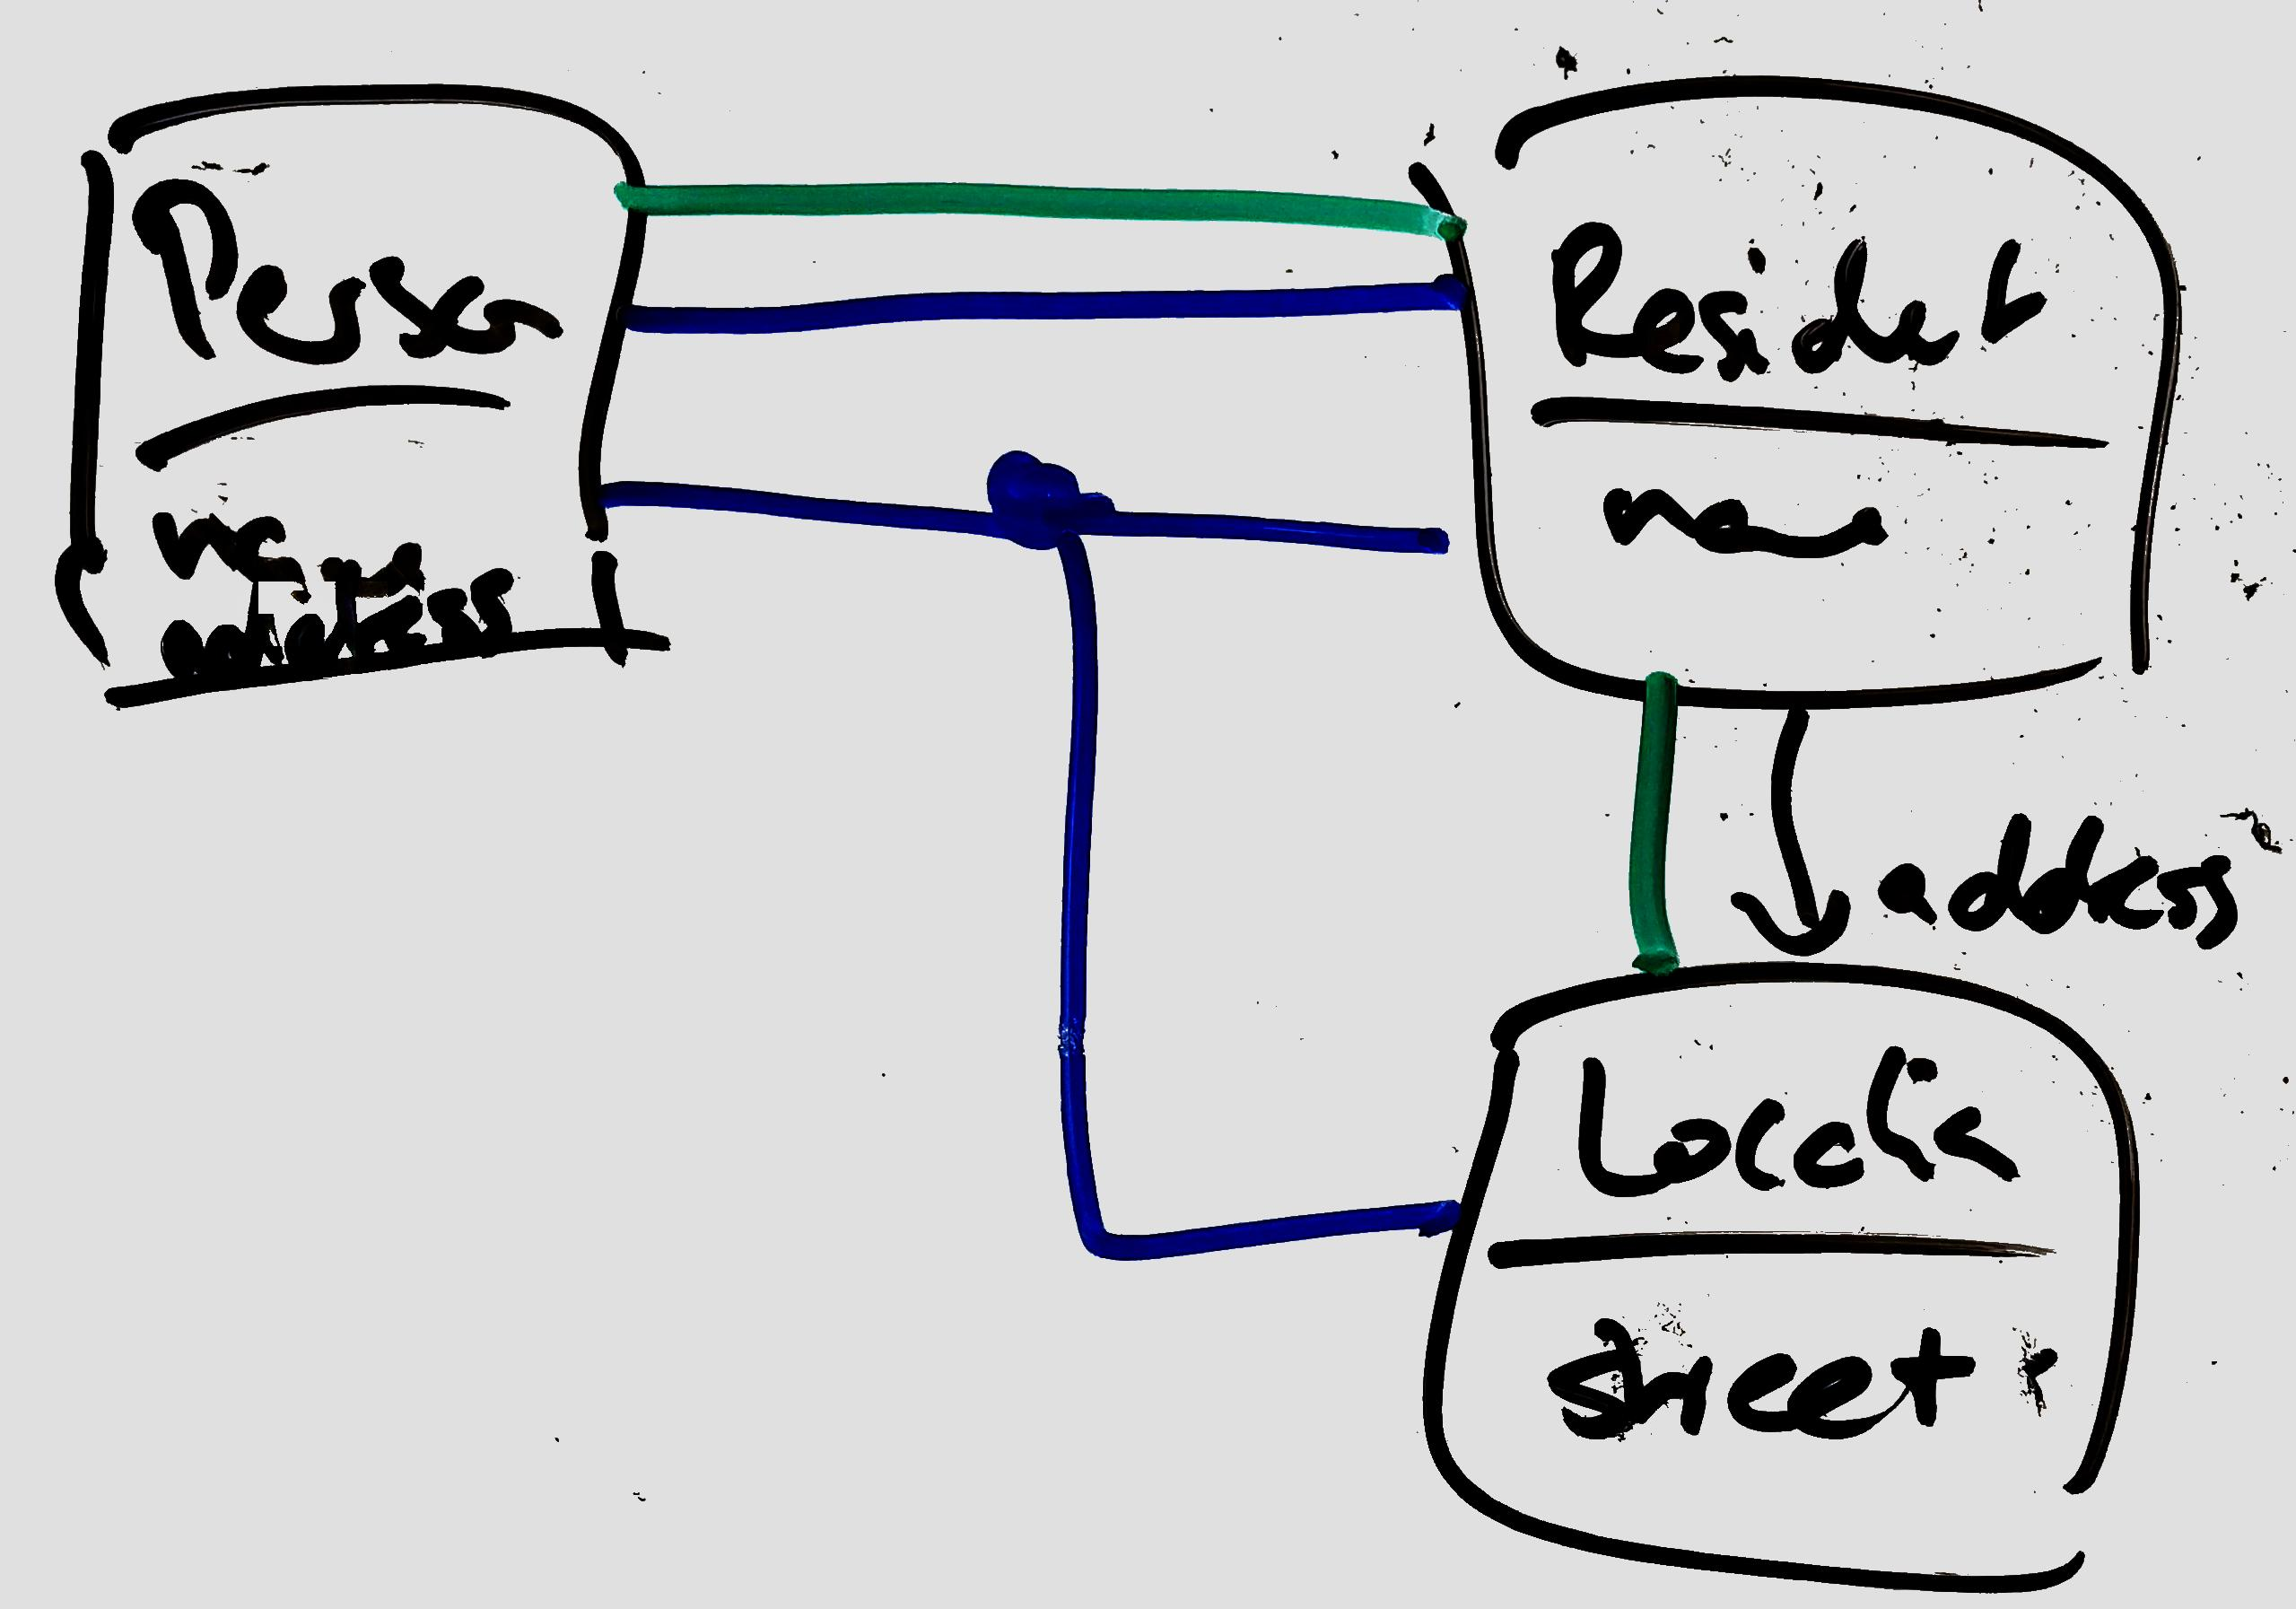
\includegraphics[width=0.5\textwidth]{figures/correctness/compatibility/hypertree.jpg}
    \caption[A hypertree with its host graph]{A hypertree (blue edges) with its host graph (green edges).}
    \label{fig:compatibility:hypertree}
\end{figure}

\mnote{Relations may be compatible if their induced hypergraphs are hypertrees}
Since consistency relations put tuple of classes into relation, it may seem natural to use a hypergraph, consisting of the classes as vertices and the class tuples of the consistency relations as hyperedges, to describe them, and expect that if the hypergraph induced by the consistency relations forms a hypertree\footnote{A hypergraph is a hypertree if there is a tree, such that every edge of the hypergraph is a set of vertices of a connected subtree of the tree~\cite{brandstaedt1998hypertrees}. Such a tree is called a \emph{host graph}.}, it is compatible.
An example for a hypertree is depicted in \autoref{fig:compatibility:hypertree}.
It consists of two hyperedges, one only relating persons and residents and one relating persons with residents and their address locations.
This is a scenario that may occur when one consistency relation puts persons and residents with their names into relation, and another describes the relation of their addresses.
These relations form a hypertree, as there is a tree, depicted in the figure, of which the vertices of all hyperedges are connected subtrees.

\mnote{Relations inducing hypertrees are not necessarily compatible}
The relations in the example may, however, not be necessarily compatible.
They can, for example, define a contradictory relation between the names of persons and residents.
In general, hypertrees induced by consistency relations are not necessarily compatible, because hyperedges can be subsets of other hyperedges and the relations inducing these hyperedges may contradict each other.
Additionally, the hyperedges to do only put sets of classes into relation and are not able distinguish between the sets belonging to different metamodels.
Thus, we have to exclude that the same classes are put into relation by multiple consistency relations in a different way.
This leads to our definition consistency relation trees.

\todoLater{Maybe we can remove symmetry and define some restriction for inverse relations. It could be useful to think about implicit relations, which are induced by another one, so that the "signatures" of forward and backward direction match.}
\begin{definition}[Consistency Relation Tree] \label{def:relationtree}
    Let $\consistencyrelationset{CR}$ be a symmetric, connected set of consistency relations. 
    %Let $\alpha = \setted{\tupled{\consistencyrelation{CR}{1}, \consistencyrelation{CR}{2}} \in \consistencyrelationset{CR} \times \consistencyrelationset{CR} \mid \classtuple{C}{r,\consistencyrelation{CR}{1}} \cap \classtuple{C}{l,\consistencyrelation{CR}{2}} \neq \emptyset \land \classtuple{C}{r,\consistencyrelation{CR}{2}} \cap \classtuple{C}{l,\consistencyrelation{CR}{1}} = \emptyset}$ be a relation on the consistency relations in $\consistencyrelationset{CR}$.
    We say:
    \begin{align*}
        &
        \consistencyrelationset{CR} \mathtextspacearound{is a consistency relation tree} \equivalentperdefinition \\
        & \formulaskip
        %\alpha \mathtext{induces a tree on} \consistencyrelationset{CR}
        \forall \consistencyrelation{CR}{} = \consistencyrelation{CR}{1} \concat \dots \concat \consistencyrelation{CR}{m}  \in \transitiveclosure{\consistencyrelationset{CR}} : \\
        & \formulaskip
        \forall \consistencyrelation{CR'}{} = \consistencyrelation{CR'}{1} \concat \dots \concat \consistencyrelation{CR'}{n} \in \transitiveclosure{\consistencyrelationset{CR}} \setminus \consistencyrelation{CR}{} : \\
        & \formulaskip\formulaskip
        \forall s, t \mid s \neq t: 
        \consistencyrelation{CR}{s} \neq \consistencyrelation{CR^T}{t} \land \consistencyrelation{CR'}{s} \neq \consistencyrelation{CR'^T}{t} \\
        & \formulaskip\formulaskip
        \Rightarrow
        \classtuple{C}{l,\consistencyrelation{CR}{}} \cap
        \classtuple{C}{l,\consistencyrelation{CR'}{}} = \emptyset
        \lor \classtuple{C}{r,\consistencyrelation{CR}{}} \cap
        \classtuple{C}{r,\consistencyrelation{CR'}{}} = \emptyset
        %
        % \forall \tupled{\consistencyrelation{CR}{1}, \dots, \consistencyrelation{CR}{k}},  \tupled{\consistencyrelation{CR'}{1}, \dots, \consistencyrelation{CR'}{m}} \in \consistencyrelationset{CR} : \\
        % & \formulaskip\formulaskip
        % \tupled{\consistencyrelation{CR}{1}, \dots, \consistencyrelation{CR}{k}} \neq \tupled{\consistencyrelation{CR'}{1}, \dots, \consistencyrelation{CR'}{m}} \\
        % & \formulaskip\formulaskip\formulaskip
        % \land \forall i, j \mid i \neq j: 
        % \consistencyrelation{CR}{i} \neq \consistencyrelation{CR^T}{j} \land \consistencyrelation{CR'}{i} \neq \consistencyrelation{CR'^T}{j} \\
        % & \formulaskip\formulaskip
        % \Rightarrow
        % \classtuple{C}{l,\consistencyrelation{CR}{1}} \cap
        % \classtuple{C}{l,\consistencyrelation{CR'}{1}} = \emptyset
        % \lor \classtuple{C}{r,\consistencyrelation{CR}{m}} \cap
        % \classtuple{C}{r,\consistencyrelation{CR'}{m}} = \emptyset
        %
        % \forall \consistencyrelation{CR}{1}, \dots, \consistencyrelation{CR}{k} \in \consistencyrelationset{CR} \mid \consistencyrelation{CR}{i} \neq \consistencyrelation{CR}{j}, \consistencyrelation{CR}{i} \neq \consistencyrelation{CR^T}{j} : \\
        % & \formulaskip\formulaskip
        % \classtuple{C}{l,\consistencyrelation{CR}{1}\concat\dots\concat\consistencyrelation{CR}{k}} \cap
        % \classtuple{C}{r,\consistencyrelation{CR}{1}\concat\dots\concat\consistencyrelation{CR}{k}} = \emptyset
        % \forall \class{C}{l} \in
        % \classtuple{C}{l,\consistencyrelation{CR}{1}\concat\dots\concat\consistencyrelation{CR}{k}} :
        % \forall \class{C}{r} \in \classtuple{C}{r,\consistencyrelation{CR}{1}\concat\dots\concat\consistencyrelation{CR}{k}}: \\
        % & \formulaskip\formulaskip
        % \class{C}{l} \cap \class{C}{r} = \emptyset
    \end{align*}
\end{definition}
\todo{We have to assume, that no element is mapped to two elements of the same class, because then it would be possible to have an incompatible network}

The definition of a consistency relation tree requires that there are no sequences of consistency relations that put the same classes into relation, i.e. between all pairs of classes there is only one concatenation of consistency relations that puts them into relation.
Since we assume a symmetric set of consistency relations, we exclude the symmetric relations from that argument, as otherwise there would always be two such concatenations by adding a consistency relation and its transposed relation to any other concatenation.

\begin{figure}
    \centering
    \input{figures/correctness/compatibility/consistency_relation_tree}
    %\includegraphics[width=\columnwidth]{figures/tree_example.png}
    \caption[A consistency relation tree]{A consistency relation tree $\setted{\consistencyrelation{CR}{1}, \consistencyrelation{CR^T}{1}, \consistencyrelation{CR}{2}, \consistencyrelation{CR^T}{2}}$. Taken from \owncite{klare2020compatibility-report}.}
    \label{fig:compatibility:tree_example}
\end{figure}

\begin{example}
\autoref{fig:compatibility:tree_example} depicts a rather simple consistency relation tree. 
Persons are related to residents and residents are related to employees, all having the same names respectively a concatenation of $firstname$ and $lastname$, by the relations $\consistencyrelation{CR}{1}, \consistencyrelation{CR}{2}$, as well as their transposed relations $\consistencyrelation{CR^T}{1}, \consistencyrelation{CR^T}{2}$.
There are no classes that are put into relation across different paths of consistency relations, thus the definition for a consistency relation tree is fulfilled. 
If an additional relation between persons and employees was specified, like in \autoref{fig:compatibility:three_persons_example_extended}, the tree definition would not be fulfilled.
\end{example}

The definition also covers the more complicated case in which multiple classes may be put into relation by consistency relations but there is only a subset of them that is put into relation by different consistency relations.
%
%\todoDiss{Subsection with discussion about why hypertrees are not suitable here}
%
We can now prove that a set of consistency relations that is a consistency relation tree is always compatible.
We first present a lemma that shows that in a consistency relation tree you can always find an order of the relations such that the classes at the right side of a relation do not overlap with the classes at the left side of a relation that preceded in the order, i.e. there is no cycle in the relations between classes.

\todo{Move this lemma and proof for tree being compatible to appendix? Is quite complicated and disturbed reading flow}
\begin{lemma}[Consistency Relation Tree Unique Paths] \label{lemma:treehassequence}
    Let $\consistencyrelationset{CR} = \setted{\consistencyrelation{CR}{1}, \consistencyrelation{CR^T}{1}, \dots, \consistencyrelation{CR}{k}, \consistencyrelation{CR^T}{k}}$ be a symmetric, connected set of consistency relations.
    $\consistencyrelationset{CR}$ is a consistency relation tree if, and only if, for each $\consistencyrelation{CR}{} \in \consistencyrelationset{CR}$ there exists a sequence of consistency relations $\sequence{\consistencyrelationset{CR}'} = \sequenced{\consistencyrelation{CR'}{1}, \dots, \consistencyrelation{CR'}{k}}$ with $\consistencyrelation{CR'}{1} = \consistencyrelation{CR}{}$, containing for each $i$ either $\consistencyrelation{CR}{i}$ or $\consistencyrelation{CR^T}{i}$, i.e.,
    \begin{align*}
        &
        \forall i \in \setted{1, \dots, k} :%\\
        %& \formulaskip 
        \bigl( \consistencyrelation{CR}{i} \in \sequence{\consistencyrelationset{CR}'} %sequenced{\consistencyrelation{CR'}{1}, \dots, \consistencyrelation{CR'}{k}}
        \land \consistencyrelation{CR^T}{i} \not\in \sequence{\consistencyrelationset{CR}'} %\sequenced{\consistencyrelation{CR'}{1}, \dots, \consistencyrelation{CR'}{k}} 
        \bigl)\\
        & \formulaskip 
        \lor \bigl(\consistencyrelation{CR^T}{i} \in \sequence{\consistencyrelationset{CR}'} %\sequenced{\consistencyrelation{CR'}{1}, \dots, \consistencyrelation{CR'}{k}}
        \land \consistencyrelation{CR}{i} \not\in \sequence{\consistencyrelationset{CR}'} %\sequenced{\consistencyrelation{CR'}{1}, \dots, \consistencyrelation{CR'}{k}} 
        \bigl)
    \end{align*}
    such that:
    \begin{align*}
        &
        %\forall \consistencyrelation{CR}{} \in \consistencyrelationset{CR} : 
        %\exists \consistencyrelation{CR'}{1}, \dots, \consistencyrelation{CR'}{k-1} \in \consistencyrelationset{CR} \setminus \setted{\consistencyrelation{CR}{}} :
        %\consistencyrelation{CR'}{i} \neq \consistencyrelation{CR'}{j}, i \neq j : \\
        \forall s \in \setted{1, \dots, k-1} : \forall t \in \setted{i+1, \dots, k} : \\
        & \formulaskip
        \classtuple{C}{r,\consistencyrelation{CR'}{s}} \cap \classtuple{C}{r,\consistencyrelation{CR'}{t}} = \emptyset 
        \land
        \classtuple{C}{l,\consistencyrelation{CR'}{s}} \cap 
        \classtuple{C}{r,\consistencyrelation{CR'}{t}} = \emptyset
        % \forall i \in \setted{1, \dots, k-1} : \\
        % & \formulaskip
        % (\exists j \in \setted{1, \dots, i-1} :  \classtuple{C}{l,\consistencyrelation{CR'}{j}} \subseteq \classtuple{C}{r,\consistencyrelation{CR'}{i}}) \\
        % & \formulaskip
        % \lor 
        % \classtuple{C}{l,\consistencyrelation{CR'}{}} \subseteq \classtuple{C}{r,\consistencyrelation{CR'}{i}}
    \end{align*}
\end{lemma}

\begin{proof}
    We start with the forward direction, i.e., given a consistency relation tree $\consistencyrelationset{CR}$ we show that there exists a sequence according to the requirements in \autoref{lemma:treehassequence} by constructing such a sequence $\sequence{\consistencyrelationset{CR}'} = \sequenced{\consistencyrelation{CR'}{1}, \dots, \consistencyrelation{CR'}{k}}$ for any $\consistencyrelation{CR}{} \in \consistencyrelationset{CR}$.
    Start with $\consistencyrelation{CR'}{1} = \consistencyrelation{CR}{}$ for any $\consistencyrelation{CR}{} \in \consistencyrelationset{CR}$.
    We now inductively add further relations to that sequence.
    Take any consistency relation $\consistencyrelation{CR}{s} = \consistencyrelation{CR}{s,1} \concat \dots \concat \consistencyrelation{CR}{s,m} \in \transitiveclosure{\consistencyrelationset{CR}}$ with $\classtuple{C}{l,\consistencyrelation{CR}{s,1}} \subseteq \classtuple{C}{r,\consistencyrelation{CR}{}}$. Such a sequence must exist because of $\consistencyrelationset{CR}$ being connected.
    Now add all $\consistencyrelation{CR}{s,1}, \dots, \consistencyrelation{CR}{s,m}$ to the sequence, such that we have $\sequenced{\consistencyrelation{CR}{}, \consistencyrelation{CR}{s,1}, \dots, \consistencyrelation{CR}{s,m}}$, which fulfills both requirements to that sequence in \autoref{lemma:treehassequence} by definition.
    The following addition of further consistency relations can be inductively applied.
    Take any other consistency relation $\consistencyrelation{CR}{t} = \consistencyrelation{CR}{t,1} \concat \dots \concat \consistencyrelation{CR}{t,n} \in \transitiveclosure{\consistencyrelationset{CR}}$ such that:
    \begin{align*}
        &
        \exists \consistencyrelation{CR'}{} \in \setted{\consistencyrelation{CR}{}, \consistencyrelation{CR}{s,1}, \dots, \consistencyrelation{CR}{s,m}} :
        \classtuple{C}{l,\consistencyrelation{CR}{t,1}} \subseteq \classtuple{C}{r,\consistencyrelation{CR'}{}}\\
        & \formulaskip
        \land
        \consistencyrelation{CR}{t,1}, \consistencyrelation{CR^T}{t,1} \not\in \setted{\consistencyrelation{CR}{}, \consistencyrelation{CR}{s,1}, \dots, \consistencyrelation{CR}{s,m}}
    \end{align*}
    In other words, take any concatenation in the transitive closure of $\consistencyrelationset{CR}$ that starts with a relation with a left class tuple that is contained in a right class tuple of a relation already added to the sequence.
    Again, such a sequence must exist because of $\consistencyrelationset{CR}$ being connected and, again, add all $\consistencyrelation{CR}{t,1}, \dots, \consistencyrelation{CR}{t,n}$ to the sequence.
    Per construction, for each $\consistencyrelation{CR'}{}$ in the sequence, there is a non-empty concatenation of relations within the sequence $\consistencyrelation{CR}{} \concat \dots \concat \consistencyrelation{CR'}{}$, because relations were added in a way that such a concatenation always exists. Since all relations in the sequence are contained in $\consistencyrelationset{CR}$, such a concatenation was also contained in $\transitiveclosure{\consistencyrelationset{CR}}$.
    First (1.), we show that the sequence still contains no duplicate elements, i.e., that none of the $\consistencyrelation{CR}{t,i}$ or $\consistencyrelation{CR^T}{t,i}$ is already contained in the sequence $\sequenced{\consistencyrelation{CR}{}, \consistencyrelation{CR}{s,1}, \dots, \consistencyrelation{CR}{s,m}}$. 
    Second (2. ,3.), we show that both further conditions for the sequence defined in \autoref{lemma:treehassequence} are still fulfilled for the sequence $\sequenced{\consistencyrelation{CR}{}, \consistencyrelation{CR}{s,1}, \dots, \consistencyrelation{CR}{s,m}, \consistencyrelation{CR}{t,1}, \dots, \consistencyrelation{CR}{t,n}}$.
    % We show that both conditions for the sequence in \autoref{lemma:treehassequence} are still fulfilled for our sequence $\tupled{\consistencyrelation{CR}{}, \consistencyrelation{CR}{s,2}, \dots, \consistencyrelation{CR}{s,m}, \consistencyrelation{CR}{t,2}, \dots, \consistencyrelation{CR}{t,n}}$ by assuming the contradictory:
    \begin{longenumerate}
        \item
    Let us assume that the sequence $\sequenced{\consistencyrelation{CR}{}, \consistencyrelation{CR}{s,1}, \dots, \consistencyrelation{CR}{s,m}}$ already contained one of the $\consistencyrelation{CR}{t,i}$ or $\consistencyrelation{CR^T}{t,i}$. If $\consistencyrelation{CR}{t,i}$ is contained in the sequence, there is a concatenation $\consistencyrelation{CR}{} \concat \dots \concat \consistencyrelation{CR}{t,i}$ with relations in $\sequenced{\consistencyrelation{CR}{}, \consistencyrelation{CR}{s,1}, \dots, \consistencyrelation{CR}{s,m}}$, as well as a concatenation $\consistencyrelation{CR}{} \concat \dots \concat \consistencyrelation{CR}{t,1} \concat \dots \concat \consistencyrelation{CR}{t,i}$.
    Since $\consistencyrelation{CR}{t,1} \not\in \setted{\consistencyrelation{CR}{}, \consistencyrelation{CR}{s,1}, \dots, \consistencyrelation{CR}{s,m}}$ by construction, these two concatenations relate the same class tuples, i.e., they contradict the definition of a consistency relation tree.
    If $\consistencyrelation{CR^T}{t,i}$ was contained in the sequence $\sequenced{\consistencyrelation{CR}{}, \consistencyrelation{CR}{s,1} \concat \dots \concat \consistencyrelation{CR}{s,m}}$, there is a concatenation $\consistencyrelation{CR}{} \concat \dots \concat \consistencyrelation{CR}{w} \concat \consistencyrelation{CR^T}{t,i}$ with relations in $\sequenced{\consistencyrelation{CR}{}, \consistencyrelation{CR}{s,1}, \dots, \consistencyrelation{CR}{s,m}}$ and, like before, the concatenation $\consistencyrelation{CR}{} \concat \dots \concat \consistencyrelation{CR}{t,1}, \dots, \consistencyrelation{CR}{t,i}$.
    Due to $\classtuple{C}{r,\consistencyrelation{CR}{w}} \cap \classtuple{C}{l,\consistencyrelation{CR}{t,i}} \neq \emptyset$ and  $\consistencyrelation{CR^T}{t,1} \not\in \setted{\consistencyrelation{CR}{}, \consistencyrelation{CR}{s,1}, \dots, \consistencyrelation{CR}{s,m}}$ by construction, the two concatenations $\consistencyrelation{CR}{} \concat \dots \concat \consistencyrelation{CR}{w}$ and $\consistencyrelation{CR}{} \concat \dots \concat \consistencyrelation{CR}{t,1} \concat \dots \concat \consistencyrelation{CR}{t,i}$ have an overlap in both their left and right class tuples, i.e., they contradict the definition of a consistency relation tree.
    In consequence, the sequence $\sequenced{\consistencyrelation{CR}{}, \consistencyrelation{CR}{s,1}, \dots, \consistencyrelation{CR}{s,m}}$ cannot have contained any $\consistencyrelation{CR}{t,i}$ or $\consistencyrelation{CR^T}{t,i}$ before.
        \item 
    Let us assume there were any $\consistencyrelation{CR'}{u}$ and $\consistencyrelation{CR'}{v}$ in the sequence $\sequenced{\consistencyrelation{CR}{}, \consistencyrelation{CR}{s,1}, \dots, \consistencyrelation{CR}{s,m}, \consistencyrelation{CR}{t,1}, \dots, \consistencyrelation{CR}{t,n}}$ such that $\classtuple{C}{r,\consistencyrelation{CR'}{u}} \cap \classtuple{C}{r,\consistencyrelation{CR'}{v}} \neq \emptyset$.
    As discussed before, for each of these relations exists a concatenation of relations in the sequence $\consistencyrelation{CR}{} \concat \dots \concat \consistencyrelation{CR'}{u}$ and $\consistencyrelation{CR}{} \concat \dots \concat \consistencyrelation{CR'}{v}$, which is contained in $\transitiveclosure{\consistencyrelationset{CR}}$.
    This contradicts the definition of a consistency relation tree, so there cannot be two such relations with overlapping classes in the right class tuple.
        \item
    Let us assume there were any $\consistencyrelation{CR'}{u}$ and $\consistencyrelation{CR'}{v}\; (u < v)$ in the sequence $\sequenced{\consistencyrelation{CR}{}, \consistencyrelation{CR}{s,1}, \dots, \consistencyrelation{CR}{s,m}, \consistencyrelation{CR}{t,1}, \dots, \consistencyrelation{CR}{t,n}}$ such that $\classtuple{C}{l,\consistencyrelation{CR'}{u}} \cap \classtuple{C}{r,\consistencyrelation{CR'}{v}} \neq \emptyset$.
    Again per construction, there must be a non-empty concatenation $\consistencyrelation{CR}{} \concat \dots \concat \consistencyrelation{CR'}{w} \concat \consistencyrelation{CR'}{u}$ with $w < u$. Since $\classtuple{C}{l,\consistencyrelation{CR'}{u}} \subseteq \classtuple{C}{r,\consistencyrelation{CR'}{w}}$ per definition, it holds that
    $\classtuple{C}{r,\consistencyrelation{CR'}{w}} \cap \classtuple{C}{r,\consistencyrelation{CR'}{v}} \neq \emptyset$.
    In other words, the relation $\consistencyrelation{CR'}{v}$ introduces a cycle in the relations.
    We have already shown in (2.) that this contradicts the definition of a consistency relation tree.
    \end{longenumerate}

    The previous strategy for adding relations to the sequence can be continued inductively by adding relations of the transitive closure of $\consistencyrelationset{CR}$ if their relations were not already added to the sequence.
    This process can be continued until finally all relations in $\consistencyrelationset{CR}$ are added to the sequence.
    Inductively applying the same arguments as before, the final sequence still fulfills all requirements for the sequence in \autoref{lemma:treehassequence}.
    % From the relations in $\consistencyrelationset{CR} \setminus \setted{\consistencyrelation{CR}, \consistencyrelation{CR^T}{}}$, we take those $\consistencyrelation{CR'}{}$ with $\classtuple{C}{l,\consistencyrelation{CR'}{}} \subseteq \classtuple{C}{r,\consistencyrelation{CR}{}}$ and add them to the sequence in an arbitrary order.
    % We recursively proceed with this procedure in a breadth-first fashion for all those added $\consistencyrelation{CR'}{}$.
    % Due to $\consistencyrelationset{CR}$ being connected by definition, this procedure finally adds all $\consistencyrelation{CR}{i}$ or $\consistencyrelation{CR^T}{i}$ to the sequence.
    % By appending always a relation to the sequence whose left class tuple is a subset of the right class tuple of an already added element, for $\consistencyrelation{CR'}{1}$ and all $\consistencyrelation{CR'}{i}$ in the sequence there is always a concatenation of a sub-sequence $\consistencyrelation{CR'}{1} \concat \dots \concat \consistencyrelation{CR'}{i}$ with non-empty left and right class tuples.
    % We show that both conditions for the sequence in \autoref{lemma:treehassequence} are fulfilled by assuming the contradictory:
    % \begin{enumerate}
    %     \item 
    % Let us assume there were any $\consistencyrelation{CR'}{s}$ and $\consistencyrelation{CR'}{t}$ in the sequence, such that $\classtuple{C}{r,\consistencyrelation{CR'}{s}} \cap \classtuple{C}{r,\consistencyrelation{CR'}{t}} \neq \emptyset$.
    % As discussed before, for both these relations there is a concatenation with non-empty left and right class tuples $\consistencyrelation{CR''}{s} = \consistencyrelation{CR'}{1} \concat \dots \concat \consistencyrelation{CR'}{s}$ and $\consistencyrelation{CR''}{t} = \consistencyrelation{CR'}{1} \concat \dots \concat \consistencyrelation{CR'}{t}$
    % such that $\classtuple{C}{l,\consistencyrelation{CR''}{s}} \cap \classtuple{C}{l,\consistencyrelation{CR''}{t}} \neq \emptyset$ and $\classtuple{C}{r,\consistencyrelation{CR''}{s}} \cap \classtuple{C}{r,\consistencyrelation{CR''}{t}} \neq \emptyset$.
    % This contradicts the definition of a consistency relation tree.
    %     \item
    % Let us assume there were any $\consistencyrelation{CR'}{s}$ and $\consistencyrelation{CR'}{t} (s < t)$ such that $\classtuple{C}{l,\consistencyrelation{CR'}{s}} \cap \classtuple{C}{r,\consistencyrelation{CR'}{t}} \neq \emptyset$.
    % Per construction, there must be a sub-sequence $\consistencyrelation{CR'}{1} \concat \dots \consistencyrelation{CR'}{u} \concat \consistencyrelation{CR'}{s}$ with $u < s$ and $\classtuple{C}{l,\consistencyrelation{CR'}{s}} \subseteq \classtuple{C}{r,\consistencyrelation{CR'}{u}}$.
    % In consequence, $\classtuple{C}{r,\consistencyrelation{CR'}{u}} \cap \classtuple{C}{r,\consistencyrelation{CR'}{s}} \neq \emptyset$.
    % We have already shown in the first case that this contradicts the definition of a consistency relation tree.
    % In other words, the relation $\consistencyrelation{CR'}{t}$ introduces a cycle in the relations.
    % \end{enumerate}
    
    We proceed with the reverse direction, i.e., given that a sequence according to the requirements in \autoref{lemma:treehassequence} exists for all $\consistencyrelation{CR}{} \in \consistencyrelationset{CR}$, we show that the set of consistency relations fulfills the definition of a consistency relation tree.
    Let us assume that the tree definition was not fulfilled, i.e., that there were two consistency relations $\consistencyrelation{CR}{s} = \consistencyrelation{CR}{s,1} \concat \dots \concat \consistencyrelation{CR}{s,m} \in \transitiveclosure{\consistencyrelationset{CR}}$ and $\consistencyrelation{CR}{t} = \consistencyrelation{CR}{t,1} \concat \dots \concat \consistencyrelation{CR}{t,n} \in \transitiveclosure{\consistencyrelationset{CR}}$ such that $\classtuple{C}{l,\consistencyrelation{CR}{s}} \cap \classtuple{C}{l,\consistencyrelation{CR}{t}} \neq \emptyset$ and $\classtuple{C}{r,\consistencyrelation{CR}{s}} \cap \classtuple{C}{r,\consistencyrelation{CR}{t}} \neq \emptyset$.
    Without loss of generality, we assume that $\consistencyrelation{CR}{s,m} \neq \consistencyrelation{CR}{t,n}$, because otherwise we could instead consider the sequence without those last relations and still fulfill the defined requirements.
    Any sequence according to \autoref{lemma:treehassequence} containing both $\consistencyrelation{CR}{s,m}$ and $\consistencyrelation{CR}{t,n}$ would contradict the assumption, because $\classtuple{C}{r,\consistencyrelation{CR}{s,m}} \cap \classtuple{C}{r,\consistencyrelation{CR}{t,n}} \neq \emptyset$ in contradiction to the assumptions regarding the sequence.
    Thus, the sequence has to contain either $\consistencyrelation{CR^T}{s,m}$ or $\consistencyrelation{CR^T}{t,n}$.
    Let us assume that the sequence contains $\consistencyrelation{CR^T}{s,m}$.
    Then the sequence cannot contain $\consistencyrelation{CR}{s,m-1}$, because $\classtuple{C}{r,\consistencyrelation{CR^T}{s,m}} \cap \classtuple{C}{r,\consistencyrelation{CR}{s,m-1}} \neq \emptyset$, which, again, would contradict the assumptions regarding the sequence.
    This argument can be inductively applied to all $\consistencyrelation{CR}{s,i}$, such that the sequence has to contain all $\consistencyrelation{CR^T}{s,i}$.
    Since the sequence contains $\consistencyrelation{CR^T}{s,1}$, it must contain $\consistencyrelation{CR}{t,1}$, because $\classtuple{C}{r,\consistencyrelation{CR^T}{s,1}} \cap \classtuple{C}{r,\consistencyrelation{CR^T}{t,1}} \neq \emptyset$.
    In consequence of $\consistencyrelation{CR}{t,1}$ being contained in the sequence, all $\consistencyrelation{CR}{t,i}$ have to be contained as well, due to the same reasons as before.
    So we have these conditions, which introduce a cycle in the overlaps of the class tuples of the relations within the sequence:
    \begin{align*}
        &
        \classtuple{C}{l,\consistencyrelation{CR^T}{s,i-1}} \cap \classtuple{C}{r,\consistencyrelation{CR^T}{s,i}} \neq \emptyset %\\ 
        %&
        \land
        \classtuple{C}{l,\consistencyrelation{CR}{t,1}} \cap \classtuple{C}{r,\consistencyrelation{CR^T}{s,1}} \neq \emptyset\\
        & 
        \land 
        \classtuple{C}{l,\consistencyrelation{CR}{t,i}} \cap \classtuple{C}{r,\consistencyrelation{CR}{t,i-1}} \neq \emptyset %\\
        %&
        \land
        \classtuple{C}{l,\consistencyrelation{CR^T}{s,m}} \cap \classtuple{C}{r,\consistencyrelation{CR}{t,n}} \neq \emptyset
    \end{align*}
    %We argued why all these relations have to be contained in the sequence.
    Because of that cycle in the overlap of class tuples, there is no order of these relations $\consistencyrelation{CR''}{1}, \dots, \consistencyrelation{CR''}{m+n}$ such that for all of them it holds that $\classtuple{C}{l,\consistencyrelation{CR''}{u}} \cap \classtuple{C}{r,\consistencyrelation{CR''}{v}} \neq \emptyset\; (u < v)$, which contradicts the assumptions regarding the sequence in \autoref{lemma:treehassequence}.
    The analog argument holds when we assume that the sequence contains $\consistencyrelation{CR^T}{t,n}$ instead of $\consistencyrelation{CR^T}{s,m}$.
    In consequence, there cannot be two such concatenations $\consistencyrelation{CR}{s}$ and $\consistencyrelation{CR}{t}$ without breaking the assumptions for the sequence in \autoref{lemma:treehassequence}.
    % Take any sequence $\tupled{\consistencyrelation{CR'}{1}, \dots, \consistencyrelation{CR'}{k}}$ with $\consistencyrelation{CR'}{1} = \consistencyrelation{CR}{s,1}$, which necessarily exists per assumption.
    % Then $\tupled{\consistencyrelation{CR}{s,1}, \dots, \consistencyrelation{CR}{s,m}}$ and $\tupled{\consistencyrelation{CR}{t,1}, \dots, \consistencyrelation{CR}{t,n}}$ are contained in $\tupled{\consistencyrelation{CR'}{1}, \dots, \consistencyrelation{CR'}{k}}$, i.e.
    % \begin{align*}
    %     \formulaskip &
    %     \forall i \in \setted{1,\dots,m-1} : 
    %     \exists v, w \in \setted{1,\dots,k} \mid v < w : \\
    %     & \formulaskip
    %     \consistencyrelation{CR}{s,i} = \consistencyrelation{CR'}{v} \land \consistencyrelation{CR}{s,i+1} = \consistencyrelation{CR'}{w}
    % \end{align*}
    % and analogously for $\tupled{\consistencyrelation{CR}{t,1}, \dots, \consistencyrelation{CR}{t,n}}$.
    % If for any $\consistencyrelation{CR}{s,i}$ there was a $\consistencyrelation{CR'}{u} \in \tupled{\consistencyrelation{CR'}{1}, \dots, \consistencyrelation{CR'}{k}}$ with $\consistencyrelation{CR}{s,i} = \consistencyrelation{CR'^T}{u}$, then 
\end{proof}

% \todoHeiko{Make this proof more precise}
% \begin{proof}
%     Let us assume the contrary, i.e. for all sequences $\tupled{\consistencyrelation{CR'}{1}, \dots, \consistencyrelation{CR'}{k}}$ according to \autoref{lemma:treehassequence}, it is true that:
%     \begin{align*}
%         \formulaskip &
%         \exists i \in \setted{1, \dots, k-1} : \\
%         & \formulaskip
%         \exists j \in \setted{i+1, \dots, k-1} :  
%         \classtuple{C}{l,\consistencyrelation{CR'}{i}} \cap 
%         \classtuple{C}{r,\consistencyrelation{CR'}{j}} \neq \emptyset
%     \end{align*}
%     Now select any such sequence $\tupled{\consistencyrelation{CR'}{1}, \dots, \consistencyrelation{CR'}{k}}$. We partition the possible sequences into two disjoint subsets and consider them independently, so this sequence falls into one of the following partitions.
%     \begin{enumerate}
%     \item Consider the following subset of sequences:
%     \begin{align*}
%         \formulaskip &
%         \exists i \in \setted{1, \dots, k-1} : \\
%         & \formulaskip
%         \forall j \in \setted{1, \dots, i-1} :  
%         \classtuple{C}{l,\consistencyrelation{CR'}{i}} \not\subseteq 
%         \classtuple{C}{r,\consistencyrelation{CR'}{j}}
%     \end{align*}
%     \todoHeiko{This is not correct. there must not be such a relation.}
%     This subset includes sequences in which there is a relation whose classes of the left condition are not a subset of the classes of any of the classes of the right condition of a previous relations in that sequence.
%     Due to $\consistencyrelationset{CR}$ being connected, for each relation $\consistencyrelation{CR'}{}$ there must be a relation $\consistencyrelation{CR''}{} \in \consistencyrelationset{CR}$, such that $\classtuple{C}{l,\consistencyrelation{CR''}{}} \subseteq \classtuple{C}{r,\consistencyrelation{CR'}{}}$. Per construction, the  sequence $\tupled{\consistencyrelation{CR'}{1}, \dots, \consistencyrelation{CR'}{k}}$ either contains such a $\consistencyrelation{CR''}{}$, or $\consistencyrelation{CR''^T}{}$.
%     If the sequence contains $\consistencyrelation{CR''}{}$, then the assumption is false by construction.
%     If the sequence contains $\consistencyrelation{CR''^T}{}$ and there is no further $\consistencyrelation{CR'''}{}$ with $\classtuple{C}{l,\consistencyrelation{CR'''}{}} \subseteq \classtuple{C}{r,\consistencyrelation{CR'}{}}$, then the assumption is also false by construction.
%     If there is such another relation, then the same argumentation applies, which inductively means that the assumption is always false.
    
%     \item Consider the following, complementary subset of sequences:
%     \begin{align*}
%         \formulaskip &
%         \forall i \in \setted{1, \dots, k-1} : \\
%         & \formulaskip
%         \exists j \in \setted{1, \dots, i-1} :  
%         \classtuple{C}{l,\consistencyrelation{CR'}{i}} \subseteq 
%         \classtuple{C}{r,\consistencyrelation{CR'}{j}}
%     \end{align*}
%     %Now select any such sequence $\tupled{\consistencyrelation{CR'}{1}, \dots, \consistencyrelation{CR'}{k}}$ in which a later relation in the relation can always be concatenated to a previous relation in the sequence:
%     If the assumption held, then there is a sequence of consistency relations $\tupled{\consistencyrelation{CR'}{1}, \dots, \consistencyrelation{CR'}{s}}$, with $\classtuple{C}{l,\consistencyrelation{CR'}{i+1}} \subseteq \classtuple{C}{r,\consistencyrelation{CR'}{i}}, i \in \setted{1, \dots, s-1}$ and
%     $\classtuple{C}{r,\consistencyrelation{CR}{s}} \cap \classtuple{C}{l, \consistencyrelation{CR}{1}} \neq \emptyset$.
%     Thus, there is the concatenation $\consistencyrelation{CR^\concat}{} = \consistencyrelation{CR'}{1} \concat \dots \concat \consistencyrelation{CR'}{s-1}$ with
%     \begin{align*}
%         \formulaskip
%         \classtuple{C}{l,\consistencyrelation{CR^\concat}{}} = \classtuple{C}{l,\consistencyrelation{CR'}{1}} \land \classtuple{C}{r,\consistencyrelation{CR^\concat}{}} \subseteq  \classtuple{C}{r,\consistencyrelation{CR'}{s-1}}
%      \end{align*}
%     per \autoref{def:relationconcatenation} for concatenation.
%     There is also the consistency relation $\consistencyrelation{CR'^T}{s} \in \consistencyrelationset{CR}$ with
%     \begin{align*}
%         \formulaskip
%         \classtuple{C}{l,\consistencyrelation{CR'^T}{s}} = \classtuple{C}{r,\consistencyrelation{CR'}{s-1}} \land  \classtuple{C}{r,\consistencyrelation{CR'^T}{s}} = \classtuple{C}{l,\consistencyrelation{CR'}{1}}
%     \end{align*}
%     such that:
%     \begin{align*}
%     \formulaskip
%         \classtuple{C}{l,\consistencyrelation{CR^\concat}{}} \cap \classtuple{C}{r,\consistencyrelation{CR'^T}{s}} \neq \emptyset \land \classtuple{C}{l,\consistencyrelation{CR'^T}{s}} \cap \classtuple{C}{r,\consistencyrelation{CR^\concat}{}} \neq \emptyset.
%     \end{align*}
%     In consequence, $\consistencyrelation{CR^\concat}{}$ and $\consistencyrelation{CR'}{}$ break the definition of a consistency relation tree.
%     \end{enumerate}
%     In combination, we have disproved the contrary statement, so we know that the statement in \autoref{lemma:treehassequence} is true.
%  \end{proof}

The previous lemma shows that the definition of consistency relation trees based on unique concatenations of the same class tuples is equivalent the possibility to find sequences of the relations that do not contain cycles in the related class tuples. %for each of the relations a sequence starting with that relation and containing all other relations as well, such that there are no cycles in the classes related by these relations.
The definition is supposed to be easier to check in practice.
However, we can now show that a consistency relation tree is always compatible with a constructive proof that requires the equivalent definition from \autoref{lemma:treehassequence}.

%With the previous lemma, we can now show that a consistency relation tree is always compatible.

\begin{theorem}[Consistency Relation Tree Compatibility] \label{theorem:treecompatibility}
    Let $\consistencyrelationset{CR}$ be a consistency relation tree, then $\consistencyrelationset{CR}$ is compatible.
\end{theorem}

\begin{figure}
    \centering
    \input{figures/correctness/compatibility/consistency_relation_tree_construction}
    %\includegraphics[width=\columnwidth]{figures/tree_construction_example.png}
    \caption[Construction of a model tuple for a consistency relation tree]{An example for constructing a model with the condition element of $\consistencyrelation{CR}{1}$ containing the person named "Alice Do" for a consistency relation tree according to the consistency relations in \autoref{fig:compatibility:tree_example}. Taken from \owncite{klare2020compatibility-report}.}
    \label{fig:compatibility:tree_construction_example}
\end{figure}

\begin{proof}
    We prove the statement by constructing a tuple of models for each condition element in the left condition of each consistency relation that contains the condition element and is consistent, i.e., that fulfills the compatibility definition.
    The basic idea is that because $\consistencyrelationset{CR}$ is a consistency relation tree, we can simply add necessary elements to get a model tuple that is consistent to all consistency relations, by %iterating through the tree in terms of 
    following an order of relations according to \autoref{lemma:treehassequence}.
    Thus, we explain an induction for constructing such a model tuple, which is also exemplified for a simple scenario in \autoref{fig:compatibility:tree_construction_example}, based on the relations in the consistency relation tree in \autoref{fig:compatibility:tree_example}.
    %First, we assume that $\consistencyrelationset{CR}$ is connected. Otherwise the following construction can be applied to the independent partitions of $\consistencyrelationset{CR}$, as their combination is compatible if each of them is compatible according to \autoref{lemma:independencecompatibility}.
    
    \paragraph{Base case:}
    Take any $\consistencyrelation{CR}{} \in \consistencyrelationset{CR}$ and any of its left side condition elements $\conditionelement{c}{l} = \tupled{\object{o}{l,1}, \dots, \object{o}{l,m}} \in \condition{c}{l, \consistencyrelation{CR}{}}$.
    %First, we construct a model set that contains $\conditionelement{c}{l}$ and is consistent to only $\consistencyrelation{CR}{}$.
    %To achieve that, 
    Select any $\conditionelement{c}{r} = \tupled{\object{o}{r,1}, \dots, \object{o}{r,n}} \in \condition{c}{r, \consistencyrelation{CR}{}}$, such that $\conditionelement{c}{l}$ and $\conditionelement{c}{r}$ constitute a consistency relation pair $\tupled{\conditionelement{c}{l}, \conditionelement{c}{r,}} \in \consistencyrelation{CR}{}$.
    %Now select any $\modelset{m} = \object{o'}{1}, \dots, \object{o'}{m+n}$, such that $\forall i \in \setted{1, \dots, n}: \object{o}{l,i} \subseteq \object{o'}{i}$ and $\forall i \in \setted{1, \dots, m}: \object{o}{r,i} \subseteq \object{o'}{n+i}$.
    Now construct the model tuple $\modeltuple{m}$ that contains only $\object{o}{l,1}, \dots, \object{o}{l,m}$ and $\object{o}{r,1}, \dots, \object{o}{r,n}$. % contains $\conditionelement{c}{l}$ and is consistent to $\consistencyrelation{CR}$ by construction.
    In consequence, we have a minimal model tuple $\modeltuple{m}$, such that $\modeltuple{m} \containsmath \conditionelement{c}{l}$ and $\modeltuple{m} \consistenttomath \consistencyrelation{CR}{}$.
    Additionally, $\modeltuple{m}$ is consistent to $\consistencyrelation{CR^T}{}$ due to symmetry of $\consistencyrelation{CR}{}$ and $\consistencyrelation{CR^T}{}$: It is $\conditionelement{c}{r} \in \condition{c}{l,\consistencyrelation{CR^T}{}}$ and $\tupled{\conditionelement{c}{r}, \conditionelement{c}{l}} \in \consistencyrelation{CR^T}{}$ and no other condition element of $\condition{c}{l,\consistencyrelation{CR^T}{}}$ is contained in $\modeltuple{m}$ by construction, thus $\modeltuple{m}$ is consistent to $\consistencyrelation{CR^T}{}$.
    In consequence, we know that for all $\consistencyrelation{CR}{} \in \consistencyrelationset{CR}$, $\setted{\consistencyrelation{CR}{}, \consistencyrelation{CR^T}{}}$ is compatible. 
    Considering the example in $\autoref{fig:compatibility:tree_construction_example}$, for the selection of any person as a condition element in $\condition{c}{l,\consistencyrelation{CR}{1}}$ (1), we select a resident in $\condition{c}{r,\consistencyrelation{CR}{1}}$ with the same name (2), such that the elements are consistent to $\consistencyrelation{CR}{1}$.
    
    \paragraph{Induction assumption:} 
    According to \autoref{lemma:treehassequence}, there is a sequence $\sequenced{\consistencyrelation{CR}{1}, \dots, \consistencyrelation{CR}{k}}$ of the relations in $\consistencyrelationset{CR}$ with $\consistencyrelation{CR}{1} = \consistencyrelation{CR}{}$, such that:
    \begin{align*}
        &
        \forall s \in \setted{1, \dots, k-1} : \forall t \in \setted{i+1, \dots, k} : \\
        & \formulaskip
        \classtuple{C}{r,\consistencyrelation{CR'}{s}} \cap \classtuple{C}{r,\consistencyrelation{CR'}{t}} = \emptyset 
        \land
        \classtuple{C}{l,\consistencyrelation{CR'}{s}} \cap 
        \classtuple{C}{r,\consistencyrelation{CR'}{t}} = \emptyset
    \end{align*}
    Considering the example in \autoref{fig:compatibility:tree_construction_example}, such a sequence would be $\sequenced{\consistencyrelation{CR}{1}, \consistencyrelation{CR}{2}}$, because the elements in the right condition of $\consistencyrelation{CR}{2}$ are not represented in the left condition of $\consistencyrelation{CR}{1}$.
    If, in general, we know that $\setted{\consistencyrelation{CR}{1}, \consistencyrelation{CR^T}{1} \dots, \consistencyrelation{CR}{i}, \consistencyrelation{CR^T}{i}}\; (i < k)$ is compatible, for every $\conditionelement{c}{l} \in \condition{C}{l,\consistencyrelation{CR}{}}$, we can find a model tuple $\modeltuple{m}$ that contains $\conditionelement{c}{l}$ and is consistent to $\setted{\consistencyrelation{CR}{1}, \consistencyrelation{CR^T}{1}, \dots, \consistencyrelation{CR}{i}, \consistencyrelation{CR^T}{i}}$ by definition.
    We can especially create a minimal model according to our construction for the base case and the following inductive completion.
    
    \paragraph{Induction step:}
    Consider $\consistencyrelation{CR}{i+1}$.
    There is at most one condition element $\conditionelement{c}{l} \in \condition{c}{l, \consistencyrelation{CR}{i+1}}$ with $\modeltuple{m} \containsmath \conditionelement{c}{l}$.
    If there were at least two condition elements $\conditionelement{c}{l}, \conditionelement{c'}{l} \in \condition{c}{l,\consistencyrelation{CR}{i+1}}$, both contained in $\modeltuple{m}$, then by construction there is a consistency relation $\consistencyrelation{CR}{s}\; (s < i+1)$ with $\conditionelement{c}{l},\conditionelement{c'}{l} \in \condition{c}{r,\consistencyrelation{CR}{j}}$.
    Let us assume there were two consistency relations $\consistencyrelation{CR}{s}, \consistencyrelation{CR}{t}$, each containing one of the condition elements in the right condition, then there would be non-empty concatenations $\consistencyrelation{CR}{} \concat \dots \concat \consistencyrelation{CR}{s}$ and $\consistencyrelation{CR'}{} \concat \dots \concat \consistencyrelation{CR}{t}$ with $\classtuple{C}{l,\consistencyrelation{CR}{}} \cap \classtuple{C}{l,\consistencyrelation{CR'}{}} \neq \emptyset$, because we started the construction with elements from the left condition of $\consistencyrelation{CR}{}$, so every element is contained because of a relation to those elements, and with $\classtuple{C}{r,\consistencyrelation{CR}{s}} \cap \classtuple{C}{r,\consistencyrelation{CR}{t}} \neq \emptyset$, because both condition elements $\conditionelement{c}{l}$ and $\conditionelement{c'}{l}$ instantiate the same classes, as they are both contained in $\condition{c}{l,\consistencyrelation{CR}{i+1}}$.
    This would violate \autoref{def:relationtree} for a consistency relation tree, thus there is only one such consistency relation $\consistencyrelation{CR}{s}$.
    Consequently, there must be two condition elements $\conditionelement{c}{ll}, \conditionelement{c'}{ll} \in \condition{c}{l,\consistencyrelation{CR}{s}}$ with $\tupled{\conditionelement{c}{ll},\conditionelement{c}{l}}, \tupled{\conditionelement{c'}{ll},\conditionelement{c'}{l}} \in \consistencyrelation{CR}{s}$, because per construction $\modeltuple{m}$ was consistent to $\consistencyrelation{CR}{s}$ and so there must be a witness structure with a unique mapping between condition elements contained in $\modeltuple{m}$.
    The above argument can be applied inductively until we finally find that there must be two condition elements $\conditionelement{c}{lll},\conditionelement{c'}{lll} \in \condition{c}{l,\consistencyrelation{CR}{}}$, which are contained in $\modeltuple{m}$.
    This is not true by construction, as we started with only one element from $\condition{c}{l,\consistencyrelation{CR}{}}$, so there is only one such condition element $\conditionelement{c}{l} \in \condition{c}{l,\consistencyrelation{CR}{i+1}}$ with $\modeltuple{m} \containsmath \conditionelement{c}{l}$.
    
    For this condition element $\conditionelement{c}{l} \in \condition{c}{l,\consistencyrelation{CR}{i+1}}$, select an arbitrary $\conditionelement{c}{r} = \tupled{\object{o}{1}, \dots, \object{o}{s}} \in \condition{c}{r, \consistencyrelation{CR}{i+1}}$, such that $\tupled{\conditionelement{c}{l}, \conditionelement{c}{r}} \in \consistencyrelation{CR}{i+1}$.
    %Now select any objects $\object{o'}{1}, \dots, \object{o'}{s}$, such that $\forall i \in \setted{1, \dots, s}: \object{o}{i} \subseteq \object{o'}{i}$ and create a model set $\modelset{m'}$ by adding the objects $\object{o'}{1}, \dots, \object{o'}{s}$ to $\modelset{m}$.
    Now create a model tuple $\modeltuple{m'}$ by adding the objects $\object{o}{1}, \dots, \object{o}{s}$ to $\modeltuple{m}$.
    Since $\conditionelement{c}{l}$ is the only of the left condition elements of $\consistencyrelation{CR}{i+1}$ that $\modeltuple{m}$ contains, model tuple $\modeltuple{m'}$ is consistent to $\consistencyrelation{CR}{i+1}$ per construction.
    $\modeltuple{m'}$ is also consistent to $\consistencyrelation{CR^T}{i+1}$, because due to the symmetry of $\consistencyrelation{CR}{i+1}$ and $\consistencyrelation{CR^T}{i+1}$, it is $\conditionelement{c}{r} \in \condition{c}{l,\consistencyrelation{CR^T}{i+1}}$ and due to $\tupled{\conditionelement{c}{r}, \conditionelement{c}{l}} \in \consistencyrelation{CR^T}{i+1}$, a consistent corresponding element exists in $\modeltuple{m'}$. 
    Furthermore, there cannot be any other $\conditionelement{c'}{} \in \condition{c}{l,\consistencyrelation{CR^T}{i+1}}$ with $\modeltuple{m'} \containsmath \conditionelement{c'}{}$, because otherwise there would have been another consistency relation $\consistencyrelation{CR'}{}$ that required the creation of $\conditionelement{c'}{}$, which means that there are two concatenations of consistency relations $\consistencyrelation{CR}{} \concat \dots \concat \consistencyrelation{CR'}{}$ and $\consistencyrelation{CR}{} \concat \dots \concat \consistencyrelation{CR}{i+1}$ that both relate instances of the same classes, which contradicts \autoref{def:relationtree} for a consistency relation tree.
    
    Additionally, due to \autoref{lemma:treehassequence}, for all  $\consistencyrelation{CR}{s}\; (s < i+1)$, we know that $\classtuple{C}{l,\consistencyrelation{CR}{s}} \cap \classtuple{C}{r,\consistencyrelation{CR}{i+1}} = \emptyset$. 
    Since the newly added elements $\conditionelement{c}{r}$ are part of $\condition{c}{r,\consistencyrelation{CR}{i+1}}$, these elements cannot match the left conditions of any of the consistency relations $\consistencyrelation{CR}{s}\; (s < i+1)$.
    So $\modeltuple{m'}$ is still consistent to all $\consistencyrelation{CR}{s}\; (s < i+1)$.
    Finally, due to \autoref{lemma:treehassequence}, for all  $\consistencyrelation{CR}{s}\; (s < i+1)$, we know that $\classtuple{C}{r,\consistencyrelation{CR}{s}} \cap \classtuple{C}{r,\consistencyrelation{CR}{i+1}} = \emptyset$.
    Again, since the newly added elements $\conditionelement{c}{r}$ are part of $\condition{c}{r,\consistencyrelation{CR}{i+1}}$, these elements cannot match the left conditions of any of the consistency relations $\consistencyrelation{CR^T}{s}\; (s < i+1)$.
    So $\modeltuple{m'}$ is still consistent to all $\consistencyrelation{CR^T}{s}\; (s < i+1)$.
    %Additionally, $\modelset{m'} \consistenttomath \consistencyrelation{CR^T}{i+1}$, because the only element of $\condition{c}{l,\consistencyrelation{CR^T}{i+1}}$ is $\conditionelement{c}{l}$. 
    %Otherwise another consistency relation would have required such an element to be updated, such there was another sequence of consistency relations next to $\consistencyrelation{CR}{}, \dots, \consistencyrelation{CR}{i+1}$ that created elements of $\classtuple{C}{r,\consistencyrelation{CR}{i+1}}$, which is not possible by \autoref{def:relationtree} for consistency relation trees.
    In consequence, we know that $\modeltuple{m'} \consistenttomath \setted{\consistencyrelation{CR}{1}, \consistencyrelation{CR^T}{1} \dots, \consistencyrelation{CR}{i+1}, \consistencyrelation{CR^T}{i+1}}$.
    
    Considering the example in \autoref{fig:compatibility:tree_construction_example}, we would select $\consistencyrelation{CR}{2}$ and add for the resident, which is in the left condition elements of $\consistencyrelation{CR}{2}$, an appropriate employee to make the model tuple consistent to $\consistencyrelation{CR}{2}$ (3).
    % If adding those elements could violate consistency to $\consistencyrelation{CR}{1}$, any element considered by $\consistencyrelation{CR}{1}$, in this case a resident, would have to be created, which is not possible, as the relations would not form a tree anymore.
    
    \paragraph{Conclusion}
    Taking the base case for $\consistencyrelation{CR}{}$ and the induction step for $\consistencyrelation{CR}{i+1}$, we have inductively shown that 
    \begin{align*}
        \formulaskip 
        \modeltuple{m'} \consistenttomath \setted{\consistencyrelation{CR}{1}, \consistencyrelation{CR^T}{1} \dots, \consistencyrelation{CR}{k}, \consistencyrelation{CR^T}{k}} = \consistencyrelationset{CR}
    \end{align*}
    Since the construction is valid for each condition element in every consistency relation in $\consistencyrelationset{CR}$, we know that a consistency relation tree $\consistencyrelationset{CR}$ is compatible.
    %
    % Now select an arbitrary $\consistencyrelation{CR'}{} \in \consistencyrelationset{CR} \setminus \setted{\consistencyrelation{CR}{}}$ with $\consistencyrelation{CR}{} \concat \consistencyrelation{CR'}{} \neq \emptyset$.
    % Such a relation must exist, because otherwise $\consistencyrelationset{CR}$ would not be connected.
    % For all condition elements $\conditionelement{c}{l} \in \condition{c}{l, \consistencyrelation{CR'}{}}$ with $\modelset{m} \containsmath \conditionelement{c}{l}$, select an arbitrary  $\conditionelement{c}{r} = \tupled{\object{o}{1}, \dots, \object{o}{s}} \in \condition{c}{r, \consistencyrelation{CR'}{}}$, such that $\tupled{\condition{c}{l, \consistencyrelation{CR'}{}}, \condition{c}{r, \consistencyrelation{CR'}{}}} \in \consistencyrelation{CR'}{}$.
    % Now select any objects $\object{o'}{1}, \dots, \object{o'}{s}$, such that $\forall i \in \setted{1, \dots, s}: \object{o}{i} \subseteq \object{o'}{i}$ and create a model set $\modelset{m'}$ by adding the objects $\object{o'}{1}, \dots, \object{o'}{s}$ to $\modelset{m}$.
    % Per construction, model set $\modelset{m'}$ is consistent to $\consistencyrelation{CR'}{}$.
    % It is also still consistent to $\consistencyrelation{CR}{}$, because if any of the newly added objects $\object{o'}{1}, \dots, \object{o'}{s}$ would violate consistency to $\consistencyrelation{CR}{}$, then there must be an overlap in the classes $\classtuple{C}{r,\consistencyrelation{CR'}{}}$ of $\consistencyrelation{CR'}{}$ and the classes $\classtuple{C}{l,\consistencyrelation{CR}{}}$ of $\consistencyrelation{CR}{}$.
    % Since $\consistencyrelation{CR}{} \concat \consistencyrelation{CR'}{} \neq \emptyset$ by construction, there is also an overlap in the class tuples $\classtuple{C}{l,\consistencyrelation{CR'}{}}$ and $\classtuple{C}{r,\consistencyrelation{CR}{}}$, so that there is a cycle in the classes, violating the definition of a consistency relation tree.
    % Considering the example in \autoref{fig:compatibility:formal:tree_construction_example}, we select $\consistencyrelation{CR}{2}$ and add an appropriate person to make the model set consistent to $\consistencyrelation{CR}{2}$ (3).
    % If adding those elements could violate consistency to $\consistencyrelation{CR}{1}$, any element considered by $\consistencyrelation{CR}{1}$, in this case a resident, would have to be created, which is not possible, as the relations would not form a tree anymore.
    %
    % Now, having added elements to make the model set $\modelset{m'}$ consistent to $\consistencyrelation{CR}{1}, \dots, \consistencyrelation{CR}{k]}$ inductively that way, select any $\consistencyrelation{CR''}{} \in \consistencyrelationset{CR} \setminus \setted{\consistencyrelation{CR}{1}, \dots, \consistencyrelation{CR}{k}}$ with $\exists i \in \setted{1, \dots, k} : \consistencyrelation{CR}{i} \concat \consistencyrelation{CR''}{} \neq \emptyset$.
    % Like before, this relation has to exist because $\consistencyrelationset{CR}$ is connected.
    % In the same way like for $\consistencyrelation{CR'}{}$, add elements to the model set $\modelset{m'}$ to form a new model set $\modelset{m''}$ that is consistent to $\consistencyrelation{CR''}{}$.
    % If these added elements would lead to $\modelset{m''}$ not being consistent to any $\consistencyrelation{CR}{1}, \dots, \consistencyrelation{CR}{k}$, due to the same argumentation as for $\consistencyrelation{CR'}{}$, there would be a sequence of consistency relations that relates one class with itself, thus $\consistencyrelationset{CR}$ would not fulfill the definition of consistency relation tree.
    % Thus, $\modelset{m''}$ is consistent to $\setted{\consistencyrelation{CR}{1}, \dots, \consistencyrelation{CR}{k}, \consistencyrelation{CR''}{}}$.
    %
    % Applying that argument inductively for all consistency relations in $\consistencyrelationset{CR}$, we are able to create a model set $\modelset{m}$ that is consistent to $\consistencyrelationset{CR}$ and that contains the initially selected condition element $\conditionelement{c}{l}$. 
    % Since the argument holds for any such condition element of any of the consistency relations, $\consistencyrelationset{CR}$ fulfills the definition of compatibility.
\end{proof}

%%
%% Summary: Independent trees are compatible
%%
Summarizing, \autoref{theorem:independencecompatibility} and \autoref{theorem:treecompatibility} have shown that consistency relation sets fulfilling a special notion of trees are compatible and that combining compatible independent sets of relations is compatibility-preserving.
In consequence, having a consistency relation set that consists of independent subsets that are consistency relation trees, this set of relations is inherently compatible.
An approach that evaluates whether a given set of consistency relations fulfills \autoref{def:independence} and \autoref{def:relationtree} for independence and trees can be used to prove compatibility of those relations.

%%
%% Transition: Actual sets may generally not be trees
%%
However, consistency relations fulfill such a structure only in specific cases.
In general, like in our motivational example in \autoref{fig:compatibility:three_persons_example_extended}, there may be different consistency relations putting the same elements into relation, such that the definition for consistency relation trees is not fulfilled.
In the following, we discuss how to find a consistency relation tree that is equivalent to a given set of consistency relations, such that this equivalence witnesses compatibility.



\subsection{Redundancy of Consistency Relations}
\label{chap:compatibility:formal_approach:redundancy}

%\todoDiss{Add a definition for a \emph{compatibility-preserving consistency relation} that states that is preserved compatibility and use that for clarifying the following lemmas and theorems.}

%%
%% Problem: Not having a compatible structure, compatibility is unclear
%%
We have introduced specific structures of consistency relations that are inherently compatible.
If a given set of consistency relations does not represent one of those structures, especially because there are multiple consistency relations putting the same classes into relation, it is unclear whether such a set is compatible.

%%
%% Idea: Find and virtually remove redundant relations
%%
In the following, we present an approach to reduce a set of consistency relations to a structure of independent consistency relation trees.
The essential idea is to find relations within the set, which do not change compatibility of the consistency relation set whether or not they are contained in it.
An approach that finds such relations and---virtually---removes them from the set until the remaining relations form a set of independent consistency relation trees, proves compatibility of the given set of relations.
We first define the term of a \emph{compatibility-preserving} relation.

\begin{definition}[Compatibility-Preserving Consistency Relation]
    \label{def:compatibilitypreserving}
    Let $\consistencyrelationset{CR}$ be a compatible set of consistency relations and let $\consistencyrelation{CR}{}$ be a consistency relation. We say that:
    \begin{align*}
        &
        \consistencyrelation{CR}{} \compatibilitypreservingtomath \consistencyrelationset{CR} \equivalentperdefinition %\\
        %& \formulaskip
        \consistencyrelationset{CR} \cup \setted{\consistencyrelation{CR}{}} \compatiblemath
    \end{align*}
\end{definition}

To be able to find such a compatibility-preserving relation, we introduce the notion of \emph{redundant} relations and prove the property of being compatibility preserving.
Informally speaking, a relation is redundant if it is expressed transitively across others, i.e., if it does not restrict or relax consistency compared to a combination of other relations.
We precisely specify a notion of redundancy in the following.

% \begin{itemize}
%     \item There may also be cycles in the fine-grained relations, such that the relation graph induced by the specification cannot witness compatibility.
%     \item If it is possible to find a set of trees that is equivalent to the given graph (\formalize{what equivalent means here!}), this serves as a witness for compatibility.
%     \item Finding such an equivalent representation can be achieved by (virtually) removing relations that have no impact on the valid instances (i.e. do not reduce the degree of consistency) (\formalize{that with the definition})
%     \item A relation is redundant if it is transitively expressed across the others, i.e. if it does not restrict the valid instances of two metamodels that are considered consistent in addition to those allowed by all other relations (\formalize{with extensional definitions of consistency}).
%     \item Virtually removing such relations leads to an equivalent representation and if that representation finally forms a tree, we have a witness for compatibility.
%     \item We explain this in detail in \autoref{sec:redundancies} and discuss how theorem proving can be used to find such redundant relations.
% \end{itemize}

\begin{definition}[Redundant Consistency Relation]
\label{def:redundancy}
    Let $\consistencyrelationset{CR}$ be a set of consistency relations for a tuple of metamodels $\metamodeltuple{M}$. %  = \setted{\metamodel{M}{1}, \dots, \metamodel{M}{k}}$.
    For a consistency relation $\consistencyrelation{CR}{} \in \consistencyrelationset{CR}$, we say that:
    \begin{align*}
        &
        \consistencyrelation{CR}{} \redundantinmath \consistencyrelationset{CR} \equivalentperdefinition %\\
        %& \formulaskip 
        \exists \consistencyrelation{CR'}{} \in \transitiveclosure{(\consistencyrelationset{CR} \setminus \setted{\consistencyrelation{CR}{}})} : 
        \forall \modeltuple{m} \in \metamodeltupleinstanceset{M} :\\
        & \formulaskip\formulaskip
        \modeltuple{m} \consistenttomath \consistencyrelation{CR'}{} \Rightarrow \modeltuple{m} \consistenttomath \consistencyrelation{CR}{}
    \end{align*}
    % \begin{align*}
    %     \formulaskip &
    %     \consistencyrelation{CR}{} \in \consistencyrelationset{CR} \mathtext{is redundant in} \consistencyrelationset{CR} \equivalentperdefinition\\
    %     & \formulaskip 
    %     \consistencyrelationset{CR} \mathtext{equivalent to} \consistencyrelationset{CR} \setminus \setted{\consistencyrelation{CR}{}}
    % \end{align*}
    % \begin{align*}
    %     \formulaskip &
    %     \consistencyrelation{CR}{} \in \consistencyrelationset{CR} \mathtext{is redundant in} \consistencyrelationset{CR} \equivalentperdefinition\\
    %     %& \formulaskip
    %     %\forall \modelset{m} = \setted{\model{m}{1}, \dots, \model{m}{k}} \mid \model{m}{i} \in \metamodelinstances{\metamodel{M}{i}} : \\
    %     & \formulaskip 
    %     \exists \consistencyrelation{CR'}{} \in \transitiveclosure{\consistencyrelationset{CR}} : \consistencyrelation{CR'}{} \mathtext{overlapping with} \consistencyrelation{CR}{} \\
    %     & \formulaskip
    %     \land \forall \consistencyrelation{CR'}{} \in \transitiveclosure{\consistencyrelationset{CR}} \mid \consistencyrelation{CR'}{} \mathtext{overlapping with} \consistencyrelation{CR}{} :\\
    %     & \formulaskip\formulaskip
    %     \bigl(\forall \tupled{\conditionelement{c}{l}, \conditionelement{c}{r}} \in \consistencyrelation{CR}{} : \exists \tupled{\conditionelement{c'}{l}, \conditionelement{c'}{r}} \in \consistencyrelation{CR'}{} : \forall \modelset{m} \in \metamodelinstances{\metamodelset{M}} : \\
    %     & \formulaskip\formulaskip\formulaskip\modelset{m} \mathtext{contains} \tupled{\conditionelement{c}{l}, \conditionelement{c}{r}} \equivalent \modelset{m} \mathtext{contains} \tupled{\conditionelement{c'}{l}, \conditionelement{c'}{r}} \\
    %     & \formulaskip\formulaskip
    %     \land \forall \tupled{\conditionelement{c'}{l}, \conditionelement{c'}{r}} \in \consistencyrelation{CR'}{} : \exists \tupled{\conditionelement{c}{l}, \conditionelement{c}{r}} \in \consistencyrelation{CR}{} : \forall \modelset{m} \in \metamodelinstances{\metamodelset{M}} : \\
    %     & \formulaskip\formulaskip\formulaskip\modelset{m} \mathtext{contains} \tupled{\conditionelement{c}{l}, \conditionelement{c}{r}} \equivalent \modelset{m} \mathtext{contains} \tupled{\conditionelement{c'}{l}, \conditionelement{c'}{r}} \bigr)
    % \end{align*}
\end{definition}

\todoLater{Add examples for redundancy! How do the elements of the redundant relation have to be related to the ones in $\consistencyrelation{CR'}{}$?}
\todoLater{Can we define an even more general notion of redundancy, not stating about the relation to a single consistency relation but the set of consistency relation, abstracting the implication to consistency to the whole set of relations?}
The definition of redundancy of a consistency relation $\consistencyrelation{CR}{}$ ensures that there is another consistency relation, possibly transitively expressed across others, such that if a model is consistent to that other relation, it is also consistent to $\consistencyrelation{CR}{}$.
This means that there are no model tuples that are considered inconsistent to $\consistencyrelation{CR}{}$, but not to another relation, thus $\consistencyrelation{CR}{}$ does not restrict consistency.
Actually, the definition of redundancy implies that the set of consistency relations with and without the redundant one are equivalent according to \autoref{def:equivalence}, thus both consider the same model tuples as consistent.

% The definition of redundancy ensures that the redundant relation does not provide any relaxation (first equivalence) or restriction (second equivalence) regarding existing consistency relations and that there is at least one overlapping consistency relation, as otherwise the relation will always restrict consistent models.
% Intuitively, redundancy could also be defined by requiring equivalence of the set of consistency relations with and without the redundant relation. In that case, exactly the same models would be considered consistent with and without the redundant relation.
% However, we want to use the redundancy definition to make statements about compatibility of sets of consistency relations, which requires this more restricted notion of redundancy.
% Actually, the definition of redundancy always implies equivalence.
\todoLater{Explain that we do not require equality of elements in CR and CR' because, e.g., CR might only related names, whereas CR' related names and addresses, thus we only require that there are elements that are co-indicating consistency.}

\begin{lemma}[Redundant Relations Equivalence] \label{lemma:redundancyimpliesequivalence}
    Let $\consistencyrelation{CR}{} \in \consistencyrelationset{CR}$ be a redundant consistency relation in a relation set $\consistencyrelationset{CR}$. %, according to \autoref{def:redundancy}.
    Then $\consistencyrelationset{CR}$ is equivalent to $\consistencyrelationset{CR} \setminus \setted{\consistencyrelation{CR}{}}$. %, according to \autoref{def:equivalence}.
\end{lemma}

\begin{proof}
    Like discussed in \autoref{lemma:consistencytransitiveclosure}, adding a consistency relation to a set of consistency relations can never lead to a relaxation of consistency, i.e., models becoming consistent that were not considered consistent before. This is a direct consequence of \autoref{def:consistency} for consistency, which requires models be consistent to all consistency relations in a set to be considered consistent, thus restricting the set of consistent model tuples by adding further consistency relations.
    In consequence, it holds that:
    \begin{align*}
        \formulaskip
        \modeltuple{m} \consistenttomath \consistencyrelationset{CR} \Rightarrow 
        \modeltuple{m} \consistenttomath \consistencyrelationset{CR} \setminus \setted{\consistencyrelation{CR}{}}
    \end{align*}
    Additionally, a direct consequence of \autoref{def:redundancy} for redundancy is that a redundant consistency relation does not restrict consistency, as it considers all models to be consistent that are also considered consistent to another consistency relation in the transitive closure of the consistency relation set. Thus, all models that are considered consistent to the transitive closure of $\consistencyrelationset{CR} \setminus \setted{\consistencyrelation{CR}{}}$ are also consistent to $\consistencyrelation{CR}{}$ and thus to all relations in $\consistencyrelationset{CR}$:
    \begin{align*}
        \formulaskip
        \modeltuple{m} \consistenttomath \transitiveclosure{(\consistencyrelationset{CR} \setminus \setted{\consistencyrelation{CR}{}})} \Rightarrow 
        \modeltuple{m} \consistenttomath \consistencyrelationset{CR}
    \end{align*}
    According to \autoref{lemma:consistencytransitiveclosure}, each tuple of models that is consistent to a consistency relation set is also consistent to its transitive closure an vice versa.
    In consequence, the previous implication is also true for $\consistencyrelationset{CR} \setminus \setted{\consistencyrelation{CR}{}}$ rather than $\transitiveclosure{(\consistencyrelationset{CR} \setminus \setted{\consistencyrelation{CR}{}})}$.
    Summarizing, $\consistencyrelationset{CR}$ and $\consistencyrelationset{CR} \setminus \setted{\consistencyrelation{CR}{}}$ are equivalent.
\end{proof}

\todoLater{Possibly add that lemma}
% \begin{lemma}
%     Let $\consistencyrelationset{CR}$ be a set of consistency relation and let $\consistencyrelation{CR}{}$ be redundant in $\consistencyrelationset{CR}$.
%     Then it holds that:
%     \begin{align*}
%         \formulaskip &
%         \exists \consistencyrelation{CR'}{} \in \transitiveclosure{\consistencyrelationset{CR}} \setminus \setted{\consistencyrelation{CR}{}} : \consistencyrelation{CR}{} \mathtext{related to} \consistencyrelation{CR'}{}\\
%         &
%         \lor \forall \modelset{m} \in \metamodelinstances{\metamodelset{M}} : \modelset{m} \mathtext{consistent to} \consistencyrelation{CR}{}
%     \end{align*}
% \end{lemma}

% \begin{proof}
%     tba \todoHeiko{Add the proof}
% \end{proof}

\begin{figure}
    \centering
    \input{figures/correctness/compatibility/redundant_relation_example}
    %\includegraphics[width=\columnwidth]{figures/redundancy_relation_extremes.png}
    \caption[Redundant consistency relation]{Redundant consistency relation $\consistencyrelation{CR}{1}$ in $\setted{\consistencyrelation{CR}{1}, \consistencyrelation{CR}{2}}$. Taken from \owncite{klare2020compatibility-report}.}
    \label{fig:compatibility:redundancyrelationextremes}
\end{figure}

In general, to consider a consistency relation redundant in %a set of consistency relation
$\consistencyrelationset{CR}$, it has to define equal or weaker requirements for consistency than one of the other relations in $\consistencyrelationset{CR}$.
Informally speaking, such weaker requirements mean that the redundant relation must have weaker conditions, i.e., it must require consistency for less objects and consider the same or more objects consistent to each of the left condition elements. %, i.e., it must have a weaker left condition, and consider the same or more elements consistent to those of the left condition.

\begin{example}
Such weaker consistency requirements are exemplified in \autoref{fig:compatibility:redundancyrelationextremes}, which shows a consistency relation $\consistencyrelation{CR}{1}$ that is redundant in $\setted{\consistencyrelation{CR}{1}, \consistencyrelation{CR}{2}}$.
A redundant consistency relation, such as $\consistencyrelation{CR}{1}$, must have weaker requirements in the left condition, such that it requires consistent elements to exist in less cases.
This means that it may have a larger set of classes that are matched and that there may be less condition elements for which consistency is required.
In case of $\consistencyrelation{CR}{1}$, the left condition contains both a resident and a location, whereas the left condition of $\consistencyrelation{CR}{2}$ only contains residents.
Thus $\consistencyrelation{CR}{1}$ requires consistent elements, i.e., employees, only if a resident and a location exists, whereas $\consistencyrelation{CR}{2}$ requires that already for an existing resident.
Furthermore, the residents for which $\consistencyrelation{CR}{1}$ defines any consistency requirements are a subset of those for which $\consistencyrelation{CR}{2}$ defines consistency requirements, as $\consistencyrelation{CR}{1}$ does not make any statements about residents having an empty name.
Thus, the left condition elements of $\consistencyrelation{CR}{1}$ are a subset of those of $\consistencyrelation{CR}{2}$.
In consequence, if $\consistencyrelation{CR}{1}$ requires consistency for a resident and a location, $\consistencyrelation{CR}{2}$ requires it anyway, because it already defines consistency for the contained resident.

Additionally, a redundant consistency relation, such as $\consistencyrelation{CR}{1}$, must have weaker requirements for the elements at the right side, such that one of the consistent right condition elements is contained anyway because another relation already required them. 
This means that the relation may have a smaller set of classes, of whom instances are required to consider the models consistent, and there may be more condition elements of the right side that are considered consistent with condition elements of the left side to not restrict the elements considered consistent.
In case of $\consistencyrelation{CR}{1}$, it only requires an employee to exist for a resident compared to $\consistencyrelation{CR}{2}$, which also requires a non-empty address to exist. Additionally, $\consistencyrelation{CR}{1}$ does not restrict the employees that are considered consistent to employees compared to $\consistencyrelation{CR}{2}$, as it also considers employees with the same name as consistent, but additionally those having the name of the resident in lowercase.
\end{example}

\todoLater{Add proposition about redundancy properties}
% These informal insights on the properties of a redundant consistency relation can be formalized as follows.

% \begin{proposition}
%     Let $\consistencyrelationset{CR}$ be a set of consistency relations and let $\consistencyrelation{CR}{}$ be a consistency relation. Then it holds that:
%     \begin{align*}
%         \formulaskip &
%         \consistencyrelation{CR}{} \redundantinmath \consistencyrelationset{CR} \cup \setted{\consistencyrelation{CR}{}} \equivalent \\
%         & \formulaskip
%         \exists \consistencyrelation{CR'}{} \in \consistencyrelationset{CR} : %\\
%         %& \formulaskip
%         \classtuple{C}{l,\consistencyrelation{CR'}{}} \subseteq \classtuple{C}{l,\consistencyrelation{CR}{}} \land
%         \classtuple{C}{r,\consistencyrelation{CR}{}} \subseteq \classtuple{C}{r,\consistencyrelation{CR'}{}} \\
%         & \formulaskip
%         \land \forall \conditionelement{c}{l} \in \condition{c}{l,\consistencyrelation{CR}{}} : \exists \conditionelement{c'}{l} \in \condition{c}{l,\consistencyrelation{CR'}{}} : \bigl( 
%         \conditionelement{c'}{l} \subseteq \conditionelement{c}{l} \\
%         & \formulaskip\formulaskip
%         \land \forall \tupled{\conditionelement{c'}{l},\conditionelement{c'}{r}} \in \consistencyrelation{CR'}{} : \exists \tupled{\conditionelement{c}{l},\conditionelement{c}{r}} \in \consistencyrelation{CR}{} : \conditionelement{c}{r} \subseteq \conditionelement{c'}{r} \big)
%     \end{align*}
% \end{proposition}

% \begin{proof}
%     tba
% \end{proof}


\begin{figure}
    \centering
    \input{figures/correctness/compatibility/redundancy_incompatible_example}
    %\includegraphics[width=\columnwidth]{figures/redundancy_compatibility_counterexample.png}
    \caption[Incompatibility with redundant consistency relation]{A consistency relation $\consistencyrelation{CR}{1}$ being redundant in  $\setted{\consistencyrelation{CR}{1}, \consistencyrelation{CR}{2}, \consistencyrelation{CR}{3}}$, with $\setted{\consistencyrelation{CR}{2}, \consistencyrelation{CR}{3}}$ being compatible and $\setted{\consistencyrelation{CR}{1}, \consistencyrelation{CR}{2},\consistencyrelation{CR}{3}}$ being incompatible. Taken from \owncite{klare2020compatibility-report}.}
    \label{fig:compatibility:redundancy_compatibility_counterexample}
\end{figure}

Our goal is to have a compatibility-preserving notion of redundancy, i.e., adding a redundant relation to a compatible relation set should preserve compatibility.
Unfortunately, our intuitive redundancy definition is not compatibility-preserving. % with our intuitive notion of redundancy, a consistency relation $\consistencyrelation{CR}{}$ that is redundant to a compatible set of consistency relations $\consistencyrelationset{CR}$ does not imply that $\consistencyrelationset{CR} \cup \setted{\consistencyrelation{CR}{}}$ is compatible.

\begin{proposition}[Redundant Relations Non-Compatibility] \label{prop:redundantnotimpliescompatible}
    Let $\consistencyrelationset{CR}$ be a compatible set of consistency relations and let $\consistencyrelation{CR}{}$ be a consistency relation that is redundant in $\consistencyrelationset{CR} \cup \setted{\consistencyrelation{CR}{}}$.
    Then $\consistencyrelation{CR}{}$ is not necessarily compatibility-preserving, i.e., $\consistencyrelationset{CR} \cup \setted{\consistencyrelation{CR}{}}$ is not necessarily compatible.
    % it holds that:
    % \begin{align*}
    %     \formulaskip &
    %     \consistencyrelationset{CR} \compatiblemath \not\Rightarrow \consistencyrelationset{CR} \cup \setted{\consistencyrelation{CR}{}} \compatiblemath
    % \end{align*}
\end{proposition}

\begin{proof}
We prove the proposition by providing a counterexample. % for the implication.
Consider the example in \autoref{fig:compatibility:redundancy_compatibility_counterexample}. 
$\consistencyrelation{CR}{2}$ relates each employee to a person with the same name and $\consistencyrelation{CR}{3}$ relates each person to a resident with the same name in lowercase.
The consistency relation set $\setted{\consistencyrelation{CR}{2}, \consistencyrelation{CR}{3}}$ is obviously compatible, because for each employee and each person, which constitute the left condition elements of the consistency relations, a consistent model tuple containing the person respectively employee can be created by adding the appropriate person or employee with the same name and a resident with the name in lowercase.
Furthermore, $\consistencyrelation{CR}{1}$ is redundant in $\setted{\consistencyrelation{CR}{1}, \consistencyrelation{CR}{2}, \consistencyrelation{CR}{3}}$ according to \autoref{def:redundancy}, because if a model is consistent to $\consistencyrelation{CR}{2}$ it is also consistent to $\consistencyrelation{CR}{1}$, since $\consistencyrelation{CR}{1}$ also requires persons with the same name as an employee to be contained in a model tuple but in less cases, precisely only those in which the model also contains a resident such that the employee name is the one of the resident in uppercase.

However, $\setted{\consistencyrelation{CR}{1}, \consistencyrelation{CR}{2}, \consistencyrelation{CR}{3}}$ is not compatible.
Intuitively, this is due to the fact that $\consistencyrelation{CR}{1}$ and $\consistencyrelation{CR}{3}$ define an incompatible mapping between the names of residents and persons.
This is also reflected by \autoref{def:compatibility} for compatibility. Take a model with an employee and a resident named $A$. This is a condition element in $\condition{c}{l,\consistencyrelation{CR}{1}}$. 
Consequentially, $\consistencyrelation{CR}{1}$ requires a person $A$ to exist. Furthermore $\consistencyrelation{CR}{3}$ requires a resident with name $a$ to exist.
In consequence, there are two tuples of employees and residents, both with employee $A$ and one with resident $A$ respectively resident $a$ each, for which a consistent person with name $A$ is required by $\consistencyrelation{CR}{1}$.
However, $\consistencyrelation{CR}{1}$ actually forbids to have two residents, one having the lowercase name of the other, because both are condition elements in $\consistencyrelation{CR}{1}$ requiring an appropriate person to occur in a consistent model, but there is only one person that to which both can be mapped, namely the one with the uppercase name, so there is no witness structure with a unique mapping as required by \autoref{def:consistency} for consistency.
This example shows that adding a redundant consistency relation to a compatible set of consistency relations does not lead to a compatible consistency relation set.
\end{proof}



\subsection{Compatibility-Preserving Redundancy}

In consequence of \autoref{prop:redundantnotimpliescompatible}, we need a stronger definition of redundancy that is compatibility-preserving. 
%to be able to derive compatibility for a consistency relation set from adding a redundant relation to an already compatible consistency relation set.
In the example in \autoref{fig:compatibility:redundancy_compatibility_counterexample} showing \autoref{prop:redundantnotimpliescompatible}, we have seen that it is problematic if a redundant consistency relation considers more classes in its left condition than the relation it is redundant to.
Therefore, we restrict the left class tuple.

\begin{definition}[Left-Equal Redundant Consistency Relation] \label{def:leftequalredundancy}
    Let $\consistencyrelationset{CR}$ be a set of consistency relations for a metamodel tuple $\metamodeltuple{M}$.
    For a consistency relation $\consistencyrelation{CR}{} \in \consistencyrelationset{CR}$, we say:
    \begin{align*}
        &
        \consistencyrelation{CR}{} \leftequalredundantinmath \consistencyrelationset{CR} \equivalentperdefinition \\
        & \formulaskip 
        \exists \consistencyrelation{CR'}{} \in \transitiveclosure{(\consistencyrelationset{CR} \setminus \setted{\consistencyrelation{CR}{}})} : 
        \forall \modeltuple{m} \in \metamodeltupleinstanceset{M} :\\
        & \formulaskip\formulaskip
        (\modeltuple{m} \consistenttomath \consistencyrelation{CR'}{} \Rightarrow \modeltuple{m} \consistenttomath \consistencyrelation{CR}{}) %\\
        %& \formulaskip\formulaskip
        \land \classtuple{C}{l,\consistencyrelation{CR}{}} = \classtuple{C}{l,\consistencyrelation{CR'}{}}
        %\consistencyrelation{CR}{} \redundantinmath \consistencyrelationset{CR} \\
        %& \formulaskip
        %\land \exists \consistencyrelation{CR'}{} \in \transitiveclosure{(\consistencyrelationset{CR} \setminus \setted{\consistencyrelation{CR}{}})} : 
        %\condition{c}{l,\consistencyrelation{CR}{}} \subseteq \condition{c}{l,\consistencyrelation{CR'}{}} 
        %\forall \conditionelement{c}{l} \in \condition{c}{l,\consistencyrelation{CR}{}} :
        %\exists \conditionelement{c'}{l} \in \condition{c}{l, \consistenyrelation{CR'}{}} :
        %\forall \modelset{m} \in \metamodelinstances{\metamodelset{M}} :
    \end{align*}
\end{definition}

%The definition of left-equal redundancy restricts the notion of redundancy to cases in which the left side of the redundant consistency relation $\consistencyrelation{CR}{}$ considers instances of the same classes as another relation in the set of consistency relations.
%As discussed before, redundancy in general allows that the left side of a redundant consistency relation $\consistencyrelation{CR}{}$ considers more classes than another relation in the set of consistency relations that induces consistency of a model set to $\consistencyrelation{CR}{}$, according to the definition of redundancy.

The definition of left-equal redundancy is similar to the redundancy definition but restricts the notion of redundancy to cases in which the left condition of the redundant consistency relation $\consistencyrelation{CR}{}$ considers the same classes than the other relation in the set of consistency relations that induces consistency of a model tuple to $\consistencyrelation{CR}{}$.
As discussed before, redundancy in general allows that the left condition of a redundant consistency relation can consider a superset of those classes. %than another relation in the set of consistency relations that induces consistency of a model set to $\consistencyrelation{CR}{}$, according to the definition of redundancy.

\begin{lemma}[Left-Equal Redundancy to Redundancy] \label{lemma:leftequalredundancyimpliesredundancy}
    Let $\consistencyrelation{CR}{}$ be a consistency relation that is left-equal redundant in a set of consistency relations $\consistencyrelationset{CR}$. Then $\consistencyrelation{CR}{}$ is redundant in $\consistencyrelationset{CR}$.
\end{lemma}

\begin{proof}
    Since the definition of left-equal redundancy is equal to the one for redundancy, apart from the additional restriction for the class tuples, redundancy of a left-equal redundant relation is a direct implication of the definition.
\end{proof}


Before showing that left-equal redundancy is compatibility-preserving, we introduce an auxiliary lemma that shows that if a model tuple contains any left condition element of a left-equal redundant relation, i.e., if that redundant relation requires the model tuple to contain corresponding elements for that object tuple to be consistent, there is also another relation that requires corresponding elements for that object tuple.

%In the following, we will show that the notion of left-equal redundancy, in comparison to the weaker general redundancy property, can be used to inductively prove compatibility of a set of consistency relations.

\begin{lemma}[Left-Equal Redundancy Containment] \label{lemma:leftequalredundancysubset}
    Let $\consistencyrelation{CR}{}$ be a consistency relation that is left-equal redundant in a set of consistency relations $\consistencyrelationset{CR}$ for a tuple of metamodels $\metamodeltuple{M}$. Then it holds that: 
    \begin{align*}
        &
        \exists \consistencyrelation{CR'}{} \in \transitiveclosure{(\consistencyrelationset{CR} \setminus \setted{\consistencyrelation{CR}{}})} : 
        \forall \conditionelement{c}{l} \in \condition{c}{l, \consistencyrelation{CR}{}} : 
        \exists \conditionelement{c'}{l} \in \condition{c}{l,\consistencyrelation{CR'}{}} : \\
        & \formulaskip
        \forall \modeltuple{m} \in \metamodeltupleinstanceset{M} : 
        \modeltuple{m} \containsmath \conditionelement{c'}{l} \Rightarrow 
        \modeltuple{m} \containsmath \conditionelement{c}{l}
    \end{align*}
\end{lemma}
%
\begin{proof}
    Due to left-equal redundancy of $\consistencyrelation{CR}{}$ in $\consistencyrelationset{CR}$, we know per definition that:
    \begin{align*}
        &
        \exists \consistencyrelation{CR'}{} \in \transitiveclosure{(\consistencyrelationset{CR} \setminus \setted{\consistencyrelation{CR}{}})} :
        \forall \modeltuple{m} \in \metamodeltupleinstanceset{M} : \\
        & \formulaskip
        \modeltuple{m} \consistenttomath \consistencyrelation{CR'}{} \Rightarrow \modeltuple{m} \consistenttomath \consistencyrelation{CR}{} \\
        & \formulaskip
        \land 
        \classtuple{C}{l,\consistencyrelation{CR}{}} = \classtuple{C}{l,\consistencyrelation{CR'}{}}
    \end{align*}
    This implies that:
    \begin{align*}
        &
        \exists \consistencyrelation{CR'}{} \in \transitiveclosure{(\consistencyrelationset{CR} \setminus \setted{\consistencyrelation{CR}{}})} :
        %\forall \modelset{m} \in \metamodelinstances{\metamodelset{M}} : \\
        %& \formulaskip
        %\condition{c}{l,\consistencyrelation{CR}{}} \subseteq \condition{c}{l,\consistencyrelation{CR'}{}} 
        \forall \conditionelement{c}{l} \in \condition{c}{l,\consistencyrelation{CR}{}} :
        \conditionelement{c}{l} \in \condition{c}{l,\consistencyrelation{CR'}{}}
    \end{align*}
    Because if there was a $\conditionelement{c}{l} \in \condition{c}{l,\consistencyrelation{CR}{}}$ so that $\conditionelement{c}{l} \not\in \condition{c}{l,\consistencyrelation{CR'}{}}$, then the model tuple $\modeltuple{m}$ only consisting of $\conditionelement{c}{l}$ would be consistent to $\consistencyrelation{CR'}{}$, because it does not require any other elements to exist for considering the model tuple consistent, whereas there is at least one $\tupled{\conditionelement{c}{l}, \conditionelement{c}{r}} \in \consistencyrelation{CR}{}$, so that $\modeltuple{m}$ needs to contain $\conditionelement{c}{r}$ for considering $\modeltuple{m}$ consistent to $\consistencyrelation{CR}{}$, which is not given by construction.
    This shows that $\condition{c}{l,\consistencyrelation{CR'}{}}$ contains all elements in $\condition{c}{l,\consistencyrelation{CR}{}}$, so there is always at least one element from $\condition{c}{l,\consistencyrelation{CR'}{}}$ that a model tuple $\modeltuple{m}$ contains if it contains an element from $\condition{c}{l,\consistencyrelation{CR}{}}$, %namely the same one, 
    which proves the statement in the lemma.
\end{proof}

\todoLater{The following lemma derived the property of left-equal redundancy from redundancy, which was not correct. Maybe we can find a more general notion of redundancy from which we can derive the contains implication, reviving this lemma gain.}
% \begin{lemma} \label{lemma:redundancysubset}
%     Let $\consistencyrelation{CR}{}$ be a consistency relation that is redundant in a set of consistency relations $\consistencyrelationset{CR}$ for a set of metamodels $\metamodelset{M}$. Thus there exists a consistency relation $\consistencyrelation{CR'}{} \in \transitiveclosure{(\consistencyrelationset{CR} \setminus \setted{\consistencyrelation{CR}{}})}$ with:
%     \begin{align*}
%         \formulaskip & 
%         \forall \modelset{m} \in \metamodelinstances{\metamodelset{M}} : \modelset{m} \consistenttomath \consistencyrelation{CR'}{} \Rightarrow \modelset{m} \consistenttomath \consistencyrelation{CR}{}
%     \end{align*}
%     Then it holds that:
%     \begin{align*}
%         \formulaskip &
%         \forall \conditionelement{c}{l} \in \condition{c}{l, \consistencyrelation{CR}{}} : \exists \conditionelement{c'}{l} \in \condition{c}{l, \consistencyrelation{CR'}{}} : 
%         \forall{m} \in \metamodelinstances{\metamodelset{M}} : \\
%         & \formulaskip
%         \modelset{m} \containsmath \condition{c'}{l} \Rightarrow \modelset{m} \containsmath \condition{c}{l} %\\
%         % &
%         % \land \forall \conditionelement{c}{r} \in \condition{c}{r, \consistencyrelation{CR}{}} : \exists \conditionelement{c'}{r} \in \condition{c}{r, \consistencyrelation{CR'}{}} : 
%         % \forall{m} \in \metamodelinstances{\metamodelset{M}} : \\
%         % & \formulaskip
%         % \modelset{m} \containsmath \condition{c'}{r} \Rightarrow \modelset{m} \containsmath \condition{c}{r}
%         %\conditionelement{c}{l} \subseteq \conditionelement{c'}{l}
%     \end{align*}
% \end{lemma}

% \begin{proof}
%     % Due to symmetry of the statement for $\conditionelement{c}{l}$ and $\conditionelement{c}{r}$, the proof is also symmetric, which is why we restrict the proof to $\conditionelement{c}{l}$. 
%     We prove that
%     \begin{align*}
%         \formulaskip &
%         \forall \conditionelement{c}{l} \in \condition{c}{l, \consistencyrelation{CR}{}} : \exists \conditionelement{c'}{l} \in \condition{c}{l, \consistencyrelation{CR'}{}} : 
%         %\forall{m} \in \metamodelinstances{\metamodelset{M}} : \\
%         %& \formulaskip
%         \conditionelement{c}{l} \subseteq \conditionelement{c'}{l}
%     \end{align*}
%     which directly implies the statement according to \autoref{def:conditionelementcontainment} for the containment of condition elements.
%     Let us assume the contrary, such that:
%     \begin{align*}
%         \formulaskip &
%         \exists \conditionelement{c}{l} \in \condition{c}{l, \consistencyrelation{CR}{}} : \forall \conditionelement{c'}{l} \in \condition{c}{l, \consistencyrelation{CR'}{}} : \conditionelement{c}{l} \not\subseteq \conditionelement{c'}{l}
%     \end{align*}
%     Consider that $\conditionelement{c}{l} = \tupled{\object{o}{1}, \dots \object{o}{n}} \in \condition{c}{l, \consistencyrelation{CR}{}}$.
%     Now select a model set $\modelset{m} \in \metamodelinstances{\metamodelset{M}}$, which only contains objects $\object{o'}{1}, \dots, \object{o'}{n}$, such that $\forall i \in \setted{1, \dots, n} : \object{o}{i} \subseteq \object{o'}{i}$. In other words, we select a minimal model set that contains $\conditionelement{c}{l}$.
%     Per definition of $\consistencyrelation{CR}{}$, there must exist at least one consistency relation pair $\tupled{\conditionelement{c}{l}, \conditionelement{c}{r}} \in \consistencyrelation{CR}{}$, in which $\conditionelement{c}{l}$ occurs.
%     Since $\modelset{m}$ does not contain any $\conditionelement{c}{r}$, $\neg (\modelset{m} \consistenttomath \consistencyrelation{CR}{})$ per definition.
%     Since $\forall \conditionelement{c'}{l} \in \condition{c}{l, \consistencyrelation{CR'}{}} : \conditionelement{c}{l} \not\subseteq \conditionelement{c'}{l}$, there is no such $\conditionelement{c'}{l}$ with $\modelset{m} \containsmath \conditionelement{c'}{l}$.
%     \dots
%     \todoHeiko{Correct and finish proof}
% \end{proof}

\begin{theorem}[Left-Equal Redundancy Compatibility] \label{theorem:redundancycompatibility}
    Let $\consistencyrelationset{CR}$ be a compatible set of consistency relations for a tuple of metamodels $\metamodeltuple{M}$ and let $\consistencyrelation{CR}{}$ be a consistency relation that is left-equal redundant in $\consistencyrelationset{CR} \cup \setted{\consistencyrelation{CR}{}}$. Then $\consistencyrelationset{CR} \cup \setted{\consistencyrelation{CR}{}}$ is compatible. 
    % If two sets of consistency relations $\set{\consistencyrelation[1]{CR}}$ and $\set{\consistencyrelation[2]{CR}}$ are equivalent and $\set{\consistencyrelation[1]{CR}}$ is compatible, then $\set{\consistencyrelation[2]{CR}}$ is compatible as well.
\end{theorem}
%
\begin{proof}
    Due to left-equal redundancy of $\consistencyrelation{CR}{}$ in $\consistencyrelationset{CR} \cup \setted{\consistencyrelation{CR}{}}$, which also implies general redundancy according to \autoref{def:redundancy}, $\consistencyrelationset{CR}$ and $\consistencyrelationset{CR} \cup \setted{\consistencyrelation{CR}{}}$ are equivalent, according to \autoref{lemma:redundancyimpliesequivalence}.
    Due to that equivalence, we know that for any model tuple $\modeltuple{m} \in \metamodeltupleinstanceset{M}$:
    \begin{equation} \label{eq:redundancyconsistency}
        \modeltuple{m} \consistenttomath \consistencyrelationset{CR} \equivalent     \modeltuple{m} \consistenttomath \consistencyrelationset{CR} \cup \setted{\consistencyrelation{CR}{}}
    \end{equation}
    It follows from \autoref{def:compatibility} for compatibility and \autoref{eq:redundancyconsistency}:
    \begin{align} \label{eq:redundancycompatibleexisting}
        & \nonumber
        \forall \consistencyrelation{CR'}{} \in \consistencyrelationset{CR} : \forall \conditionelement{c}{l} \in \condition{c}{l, \consistencyrelation{CR'}{}} %\cup \condition{c}{r, \consistencyrelation{CR'}{}} 
        : \exists \modeltuple{m} \in \metamodeltupleinstanceset{M} : \\
        & \formulaskip
        \modeltuple{m} \containsmath \conditionelement{c}{l} \land \modeltuple{m} \containsmath \consistencyrelationset{CR} \cup \setted{\consistencyrelation{CR}{}}
    \end{align}
    This already shows that for $\consistencyrelationset{CR}$ the compatibility definition is fulfilled, so we need to prove that the compatibility definition is fulfilled for $\consistencyrelation{CR}{}$ as well.
    % \begin{align*}
    %     \formulaskip &
    %     \forall \tupled{\conditionelement{c}{l}, \conditionelement{c}{r}} \in \consistencyrelation{CR}{} : \exists \modelset{m} \in \metamodelinstances{\metamodelset{M}}: \\
    %     & \formulaskip
    %     \modelset{m} \mathtext{contains} \tupled{\conditionelement{c}{l}, \conditionelement{c}{r}} \land \modelset{m} \mathtext{consistent to} \consistencyrelationset{CR} \cup \setted{\consistencyrelation{CR}{}}
    % \end{align*}
    Due to compatibility of $\consistencyrelationset{CR}$ and \autoref{lemma:compatibilitytransitiveclosure} showing equality of compatibility for a consistency relation set and its transitive closure, we know that:
    \begin{align} \label{eq:compatibilityclosure}
        & \nonumber
        \forall \consistencyrelation{CR'}{} \in \transitiveclosure{\consistencyrelationset{CR}} : \forall \conditionelement{c}{l} \in \condition{c}{l, \consistencyrelation{CR'}{}} %\cup \condition{c}{r, \consistencyrelation{CR'}{}} 
        : \exists \modeltuple{m} \in \metamodeltupleinstanceset{M} : \\
        & \formulaskip
        \modeltuple{m} \containsmath \conditionelement{c}{l} \land \modeltuple{m} \consistenttomath \transitiveclosure{\consistencyrelationset{CR}}
    \end{align}
    Due to left-equal redundancy of $\consistencyrelation{CR}{}$ in $\consistencyrelationset{CR} \cup \setted{\consistencyrelation{CR}{}}$, we have shown in \autoref{lemma:leftequalredundancysubset} that the following is true:
    \begin{align} \label{eq:redundancycontainment}
        & \nonumber 
        \exists \consistencyrelation{CR'}{} \in \transitiveclosure{\consistencyrelationset{CR}} : \forall \conditionelement{c}{l} \in \condition{c}{l, \consistencyrelation{CR}{}} : \exists \conditionelement{c'}{l} \in \condition{c}{l,\consistencyrelation{CR'}{}} : \forall \modeltuple{m} \in \metamodeltupleinstanceset{M} : \\
        & \formulaskip
        \modeltuple{m} \containsmath \conditionelement{c'}{l} \Rightarrow \modeltuple{m} \containsmath \conditionelement{c}{l}
    \end{align}
    The combination of \autoref{eq:compatibilityclosure} and \autoref{eq:redundancycontainment} gives:
    \begin{align*}
        & \nonumber 
        \exists \consistencyrelation{CR'}{} \in \transitiveclosure{\consistencyrelationset{CR}} : \forall \conditionelement{c}{l} \in \condition{c}{l, \consistencyrelation{CR}{}} : \exists \conditionelement{c'}{l} \in \condition{c}{l,\consistencyrelation{CR'}{}} : \\
        & \formulaskip
        (\forall \modeltuple{m} \in \metamodeltupleinstanceset{M} : \modeltuple{m} \containsmath \conditionelement{c'}{l} \Rightarrow \modeltuple{m} \containsmath \conditionelement{c}{l}) \\
        & \formulaskip
        \land (\exists \modeltuple{m} \in \metamodeltupleinstanceset{M} :
        \modeltuple{m} \containsmath \conditionelement{c'}{l} \land \modeltuple{m} \consistenttomath \transitiveclosure{\consistencyrelationset{CR}})
    \end{align*}
    A simplification by combining the two last lines of that statement leads to:
    \begin{align*}
        & \nonumber 
        \forall \conditionelement{c}{l} \in \condition{c}{l, \consistencyrelation{CR}{}} : \exists \modeltuple{m} \in \metamodeltupleinstanceset{M} : \\
        & \formulaskip
        \modeltuple{m} \containsmath \conditionelement{c}{l} \land \modeltuple{m} \consistenttomath \transitiveclosure{\consistencyrelationset{CR}}
    \end{align*}
    Due to \autoref{eq:redundancyconsistency} and \autoref{lemma:consistencytransitiveclosure}, which shows equality of consistency for a consistency relation set and its transitive closure, this is equivalent to:
    \begin{align} \label{eq:redundancycompatiblenew}
        & \nonumber 
        \forall \conditionelement{c}{l} \in \condition{c}{l, \consistencyrelation{CR}{}} : \exists \modeltuple{m} \in \metamodeltupleinstanceset{M} : \\
        & \formulaskip
        \modeltuple{m} \containsmath \conditionelement{c}{l} \land \modeltuple{m} \consistenttomath \consistencyrelationset{CR} \cup \setted{\consistencyrelation{CR}{}}
    \end{align}
    % Together with the symmetric argumentation for $\conditionelement{c}{r}$ rather than $\conditionelement{c}{l}$, we have shown that the compatibility definition holds for $\consistencyrelation{CR}{}$:
    % \begin{align} \label{eq:redundancycompatiblenew}
    %     \formulaskip & \nonumber 
    %     \forall \conditionelement{c}{} \in \condition{c}{l, \consistencyrelation{CR}{}} \cup \condition{c}{r,\consistencyrelation{CR}{}}: \exists \modelset{m} \in \metamodelinstances{\metamodelset{M}} : \\
    %     & \formulaskip
    %     \modelset{m} \mathtext{contains} \conditionelement{c}{} \land \modelset{m} \mathtext{consistent to} \consistencyrelationset{CR} \cup \setted{\consistencyrelation{CR}{}}
    % \end{align}
    The combination of \autoref{eq:redundancycompatibleexisting} and \autoref{eq:redundancycompatiblenew} shows that $\consistencyrelationset{CR} \cup \setted{\consistencyrelation{CR}{}}$ fulfills \autoref{def:compatibility} for compatibility.
    % Assume that given equivalent consistency relation sets $\set{\consistencyrelation[1]{CR}}$ and $\set{\consistencyrelation[2]{CR}}$ are equivalent and $\set{\consistencyrelation[1]{CR}}$ is compatible, whereas $\set{\consistencyrelation[2]{CR}}$ is not.
    % Then there is a consistency relation $\consistencyrelation{CR} \in \set{\consistencyrelation[2]{CR}}$ such that for all pairs of tuples $\bigtupled{\tupled{e_{l1}, \ldots, e_{ln}}, \tupled{e_{r1}, \ldots, e{rm}}} \in \consistencyrelation{CR}$ there is no set of models $\tupled{\model[1]{m}, \ldots, \model[k]{m}}$ such that for all models $\model[i]{m}, \model[j]{m}$ in that tuple either (i) $\{e_{l1}, \ldots e_{ln} \} \not\subseteq \model[i]{m} \lor \{e_{r1}, \ldots e_{rm} \not\subseteq \model[j]{m}$ or (ii) $\{ \model[1]{m}, \ldots, \model[k]{m} \} \text{not consistent according to} \set{\consistencyrelation[2]{CR}} \setminus \{ \consistencyrelation{CR} \}$. 
\end{proof}

% \begin{proof}
%     %In the proof, we always consider model sets $\modelset{m}$ to be sets of instances of the metamodels that are related by the consistency relations in $\consistencyrelationset{CR} \cup \setted{\consistencyrelation{CR}{}}$, without further mentioning that.
%     Due to the redundancy of $\consistencyrelation{CR}{}$ in $\consistencyrelationset{CR} \cup \setted{\consistencyrelation{CR}{}}$, $\consistencyrelationset{CR}$ and $\consistencyrelationset{CR} \cup \setted{\consistencyrelation{CR}{}}$ are equivalent, according to \autoref{corollary:redundancyimpliedequivalence}.
%     Due to that equivalence, it holds that for any model set $\modelset{m}$:
%     \begin{equation} \label{eq:redundancyconsistency}
%     \formulaskip 
%     \modelset{m} \mathtext{consistent to} \consistencyrelationset{CR} \equivalent \modelset{m} \mathtext{consistent to} \consistencyrelationset{CR} \cup \setted{\consistencyrelation{CR}{}}
%     \end{equation}
%     Due to \autoref{def:compatibility} for compatibility and \autoref{eq:redundancyconsistency}, it holds that:
%     \begin{align} \label{eq:redundancycompatibleexisting}
%         \formulaskip & \nonumber
%         \forall \consistencyrelation{CR'}{} \in \consistencyrelationset{CR} : \forall \tupled{\conditionelement{c}{l}, \conditionelement{c}{r}} \in \consistencyrelation{CR'}{} : \exists \modelset{m} \in \metamodelinstances{\metamodelset{M}}: \\
%         & \formulaskip
%         \modelset{m} \mathtext{contains} \tupled{\conditionelement{c}{l}, \conditionelement{c}{r}} \land \modelset{m} \mathtext{consistent to} \consistencyrelationset{CR} \cup \setted{\consistencyrelation{CR}{}}
%     \end{align}
%     This already shows that for $\consistencyrelationset{CR}$ the compatibility definition holds, so we need to prove that the compatibility definition holds for $\consistencyrelation{CR}{}$.
%     % \begin{align*}
%     %     \formulaskip &
%     %     \forall \tupled{\conditionelement{c}{l}, \conditionelement{c}{r}} \in \consistencyrelation{CR}{} : \exists \modelset{m} \in \metamodelinstances{\metamodelset{M}}: \\
%     %     & \formulaskip
%     %     \modelset{m} \mathtext{contains} \tupled{\conditionelement{c}{l}, \conditionelement{c}{r}} \land \modelset{m} \mathtext{consistent to} \consistencyrelationset{CR} \cup \setted{\consistencyrelation{CR}{}}
%     % \end{align*}
%     Due to compatibility of $\consistencyrelationset{CR}$ and \autoref{lemma:compatibilitytransitiveclosure} and \autoref{lemma:consistencytransitiveclosure}, it holds that:
%     \begin{align} \label{eq:compatibilityclosure}
%         \formulaskip & \nonumber
%         \forall \consistencyrelation{CR'}{} \in \transitiveclosure{\consistencyrelationset{CR}} : \forall \tupled{\conditionelement{c'}{l}, \conditionelement{c'}{r}} \in \consistencyrelation{CR'}{} : \exists \modelset{m} \in \metamodelinstances{\metamodelset{M}} :\\
%         & \formulaskip
%         \modelset{m} \mathtext{contains} \tupled{\conditionelement{c'}{l}, \conditionelement{c'}{r}} \land \modelset{m} \mathtext{consistent to} \transitiveclosure{\consistencyrelationset{CR}}
%     \end{align}
%     Due to the redundancy of $\consistencyrelation{CR}{}$ in $\consistencyrelationset{CR} \cup \setted{\consistencyrelation{CR}{}}$, it holds that:
%     \begin{align} \label{eq:redundancycontainment}
%         \formulaskip & \nonumber 
%         \exists \consistencyrelation{CR'}{} \in \transitiveclosure{\consistencyrelationset{CR}} : \forall \tupled{\conditionelement{c}{l}, \conditionelement{c}{r}} \in \consistencyrelation{CR}{} : \exists \tupled{\conditionelement{c'}{l}, \conditionelement{c'}{r}} \in \consistencyrelation{CR'}{} : \forall \modelset{m} \in \metamodelinstances{\metamodelset{M}} : \\
%         & \formulaskip 
%         \modelset{m} \mathtext{contains} \tupled{\conditionelement{c}{l}, \conditionelement{c}{r}} \equivalent
%         \modelset{m} \mathtext{contains} \tupled{\conditionelement{c'}{l}, \conditionelement{c'}{r}}
%     \end{align}
%     \autoref{eq:compatibilityclosure} especially holds for the selected $\consistencyrelation{CR'}{}$ and $\tupled{\conditionelement{c'}{l}, \conditionelement{c'}{r}}$ in \autoref{eq:redundancycontainment}, such that the following holds:
%     \begin{align*}
%         \formulaskip & 
%         \exists \consistencyrelation{CR'}{} \in \transitiveclosure{\consistencyrelationset{CR}} : \forall \tupled{\conditionelement{c}{l}, \conditionelement{c}{r}} \in \consistencyrelation{CR}{} : \exists \tupled{\conditionelement{c'}{l}, \conditionelement{c'}{r}} \in \consistencyrelation{CR'}{} : \\
%         & \formulaskip 
%         \forall \modelset{m} \in \metamodelinstances{\metamodelset{M}} : \modelset{m} \mathtext{contains} \tupled{\conditionelement{c}{l}, \conditionelement{c}{r}} \equivalent
%         \modelset{m} \mathtext{contains} \tupled{\conditionelement{c'}{l}, \conditionelement{c'}{r}} \\
%         & \formulaskip
%         \land \exists \modelset{m} \in \metamodelinstances{\metamodelset{M}} : \modelset{m} \mathtext{contains} \tupled{\conditionelement{c'}{l}, \conditionelement{c'}{r}} \land \modelset{m} \mathtext{consistent to} \transitiveclosure{\consistencyrelationset{CR}}
%     \end{align*}
%     Combining the last two lines leads to:
%     \begin{align*}
%         \formulaskip & 
%         \exists \consistencyrelation{CR'}{} \in \transitiveclosure{\consistencyrelationset{CR}} : \forall \tupled{\conditionelement{c}{l}, \conditionelement{c}{r}} \in \consistencyrelation{CR}{} : \exists \tupled{\conditionelement{c'}{l}, \conditionelement{c'}{r}} \in \consistencyrelation{CR'}{} : \\
%         & \formulaskip
%         \exists \modelset{m} \in \metamodelinstances{\metamodelset{M}} : \modelset{m} \mathtext{contains} \tupled{\conditionelement{c}{l}, \conditionelement{c}{r}} \land \modelset{m} \mathtext{consistent to} \transitiveclosure{\consistencyrelationset{CR}}
%     \end{align*}
%     This implies with \autoref{lemma:consistencytransitiveclosure} and \autoref{eq:redundancyconsistency} that:
%     \begin{align} \label{eq:redundancycompatiblenew}
%         \formulaskip & \nonumber
%         \forall \tupled{\conditionelement{c}{l}, \conditionelement{c}{r}} \in \consistencyrelation{CR}{} : \exists \modelset{m} \in \metamodelinstances{\metamodelset{M}} : \\
%         & \formulaskip
%         \modelset{m} \mathtext{contains} \tupled{\conditionelement{c}{l}, \conditionelement{c}{r}} \land \modelset{m} \mathtext{consistent to} \consistencyrelationset{CR} \cup \setted{\consistencyrelation{CR}{}}
%     \end{align}
%     The combination of \autoref{eq:redundancycompatibleexisting} and \autoref{eq:redundancycompatiblenew} shows that the compatibility definition is fulfilled for $\consistencyrelationset{CR} \cup \setted{\consistencyrelation{CR}{}}$.
%     % Assume that given equivalent consistency relation sets $\set{\consistencyrelation[1]{CR}}$ and $\set{\consistencyrelation[2]{CR}}$ are equivalent and $\set{\consistencyrelation[1]{CR}}$ is compatible, whereas $\set{\consistencyrelation[2]{CR}}$ is not.
%     % Then there is a consistency relation $\consistencyrelation{CR} \in \set{\consistencyrelation[2]{CR}}$ such that for all pairs of tuples $\bigtupled{\tupled{e_{l1}, \ldots, e_{ln}}, \tupled{e_{r1}, \ldots, e{rm}}} \in \consistencyrelation{CR}$ there is no set of models $\tupled{\model[1]{m}, \ldots, \model[k]{m}}$ such that for all models $\model[i]{m}, \model[j]{m}$ in that tuple either (i) $\{e_{l1}, \ldots e_{ln} \} \not\subseteq \model[i]{m} \lor \{e_{r1}, \ldots e_{rm} \not\subseteq \model[j]{m}$ or (ii) $\{ \model[1]{m}, \ldots, \model[k]{m} \} \text{not consistent according to} \set{\consistencyrelation[2]{CR}} \setminus \{ \consistencyrelation{CR} \}$. 
    
%     % Need to redefine compatibility to proceed \dots
% \end{proof}
% \todoHeiko{the proof does not require the second part of the redundancy definition, so can we omit it? Or is there a mistake in the proof?}

\begin{corollary}[Transitive Redundancy Compatibility] \label{corollary:transitiveredundancycompatibility}
    Let $\consistencyrelationset{CR}$ be a compatible set of consistency relations and let $\consistencyrelation{CR}{1}, \dots, \consistencyrelation{CR}{k}$ be consistency relations with:
    \begin{align*}
        &
        \forall i \in \setted{1, \dots, k} : %\\
        %& \formulaskip 
        \consistencyrelation{CR}{i} \leftequalredundantinmath \consistencyrelationset{CR} \cup \setted{\consistencyrelation{CR}{1}, \dots, \consistencyrelation{CR}{i}}
    \end{align*}
    Then $\consistencyrelationset{CR} \cup \setted{\consistencyrelation{CR}{1}, \dots, \consistencyrelation{CR}{k}}$ is compatible.
\end{corollary}

\begin{proof}
    This is an inductive implication of \autoref{theorem:redundancycompatibility}, because $\consistencyrelationset{CR}$ is compatible and sequentially adding $\consistencyrelation{CR}{i}$ to $\consistencyrelationset{CR} \cup \setted{\consistencyrelation{CR}{1}, \dots, \consistencyrelation{CR}{i-1}}$ ensures that $\consistencyrelationset{CR} \cup \setted{\consistencyrelation{CR}{1}, \dots, \consistencyrelation{CR}{i}}$ is compatible, because $\consistencyrelationset{CR} \cup \setted{\consistencyrelation{CR}{1}, \dots, \consistencyrelation{CR}{i-1}}$ was compatible as well.
\end{proof}

With \autoref{corollary:transitiveredundancycompatibility}, we have shown that if we have a set of consistency relations $\consistencyrelationset{CR}$ and are able to find a sequence of redundant consistency relations $\consistencyrelation{CR}{1}, \dots {\consistencyrelation{CR}{k}}$ according to \autoref{corollary:transitiveredundancycompatibility} such that we know that $\consistencyrelationset{CR} \setminus \setted{ \consistencyrelation{CR}{1}, \dots {\consistencyrelation{CR}{k}}}$ is compatible, then it is proven that $\consistencyrelationset{CR}$ is compatible.



\subsection{An Algorithm to Prove Compatibility} % Trees, Independence and Redundancy for Witnessing Compatibility
\label{chap:compatibility:formal_approach:algorithm}

In the previous sections, we have proven the following three central insights:
\begin{longenumerate}
    \item Compatibility is composable: If independent sets of consistency relations are compatible, then their union is compatible as well (\autoref{theorem:independencecompatibility}).
    \item Consistency relation trees are compatible: If there are no two concatenations of consistency relations in a consistency relation set that relate the same classes, then that set is compatible (\autoref{theorem:treecompatibility}).
    \item Left-equal redundancy is compatibility-preserving: Adding a left-equal redundant consistency relation to a compatible set of consistency relations, that set unified with the redundant relation is still compatible (\autoref{corollary:transitiveredundancycompatibility}).
\end{longenumerate}

These insights enable us to define a formal approach for proving compatibility of a set of consistency relations.
Given a set of relations for which compatibility shall be proven, we search for consistency relations in that set that are left-equal redundant to it.
If iteratively removing such redundant relations---virtually---from the set leads to a set of independent consistency relation trees, it is proven that the initial set of consistency relations is compatible.

\begin{algorithm}
    \input{algorithms/correctness/compatibility/formal_compatibility_algorithm.tex}
    \caption[Proof for compatibility of consistency relations]{Proof for compatibility of consistency relations.}
    \label{algo:compatibility}
\end{algorithm}

An algorithm that realizes this procedure is given in \autoref{algo:compatibility}.
It executes the described steps and assumes appropriate procedures to find out whether the given set of relations is a relation tree, whether it consists of independent subsets and whether there it contains a redundant relations.
It is easy to see that this algorithm is correct, as is implements the proven findings of the previous sections.
This does, however, not mean that implementing the sub-procedures is trivial.
We will provide a practical approach to realize them in the subsequent section.

\begin{theorem}[Compatibility Algorithm Correctness]
    \label{theorem:compatibilityalgorithmcorrectness}
    \autoref{algo:compatibility} is correct, i.e., it only returns \textsc{true} if the given consistency relations set $\consistencyrelationset{CR}$ is actually compatible.
\end{theorem}

\begin{proof}
    We make a case distinction for the situation in which the algorithm returns a result:
    \begin{longenumerate}
        \item When the consistency relation set is a tree, the algorithm directly returns \textsc{true} (Lines \ref{algo:compatibility:starttree}--\ref{algo:compatibility:endtree}), which is correct according to \autoref{theorem:treecompatibility}.
        \item When the consistency relation set can be split into independent sets, the algorithm returns \textsc{true} when both independent sets are identified as compatible by recursive application of the algorithm (Lines \ref{algo:compatibility:startindependence}--\ref{algo:compatibility:endindependence}), which is correct according to \autoref{theorem:independencecompatibility}.
        \item When the consistency relation set contains a redundant relation, the algorithm returns \textsc{true} when the set without the redundant relation is identified as compatible by recursive application of the algorithm (Lines \ref{algo:compatibility:startredundancy}--\ref{algo:compatibility:endredundancy}), which is correct according to \autoref{corollary:transitiveredundancycompatibility}.
        \item In all other cases, the algorithm returns \textsc{false} (Line \ref{algo:compatibility:failure}).
        \qedhere
    \end{longenumerate}
\end{proof}

The algorithm is, however, also \emph{conservative}.
%Such an approach to prove compatibility of consistency relations is \emph{conservative}.
If the approach finds redundant relations, such that a consistency relation set can be reduced to a set of independent consistency relations trees, the set is proven compatible, as we have shown by proof.
If the approach is not able to find such relations, the set may still be compatible, but the approach is not able to prove that.
Conceptually, this can be due to the fact that there may be compatibility-preserving relations that do not fulfill the definition of left-equal redundancy.
Furthermore, an actual technique to identify left-equal redundant relations may not be able to find all of them automatically, as we will see later.

\begin{theorem}[Compatibility Algorithm Conservativeness]
    \autoref{algo:compatibility} is conservative, i.e., it is correct, but if it returns \textsc{false} the given consistency relations set $\consistencyrelationset{CR}$ is not necessarily incompatible.
\end{theorem}

\begin{proof}
    We know that the algorithm is correct due to \autoref{theorem:compatibilityalgorithmcorrectness}.
    Additionally, it is easy to find examples for which the algorithm cannot prove compatibility, although the relations are compatible.
    Let us assume a consistency relation $\consistencyrelation{CR}{}$. 
    Then we construct a consistency relation $\consistencyrelation{CR}{}'$ by taking $\consistencyrelation{CR}{}$, adding an arbitrary class $C$ to the left-hand side class tuple of the relation and constructing the relation elements by taking the ones in $\consistencyrelation{CR}{}$, each complemented by all instances of $C$.
    Then $\setted{\consistencyrelation{CR}{},\consistencyrelation{CR}{}'}$ is, by construction, compatible, but the two relations are neither independent or a consistency relation tree, as they relate the same classes, nor are they redundant according to \autoref{def:leftequalredundancy}, because the left-side class tuples are not equal.
\end{proof}

The example given in the proof for conservativeness shows that the strictness of our definition for left-equal redundancy (\autoref{def:leftequalredundancy}).
We will, however, see in the evaluation that it is still sufficient in realistic cases, although such special cases as discussed in the proof are not supported.

In the following, we discuss how such an approach can be operationalized.
First, we discuss how actual transformations, at the example of \qvtr, can be represented in a graph-based structure, such that it conforms to our formal notion and allows to check whether the structure is an independent set of consistency relation trees.
Second, we present an approach for finding consistency relations that are left-equal redundant, by the means of an SMT solver applied to the constraints defined in \qvtr relations.


\todoLater{We partly did that by the expressiveness section for model-level and fine grained relations: Construction of valid models. Valid models may restrict the usable instances of a metamodel. Discuss impact on definitions and theorems and especially the constructive discussions within the proofs. Especially consider the meaning of references in models.}

%\subsection{TODO}
%\begin{itemize}
%    \item Afterthought: Construction of valid models. Valid models may restrict the usable instances of a metamodel. Discuss impact on definitions and theorems and especially the constructive discussions within the proofs. Especially consider the meaning of references in models.
%    \item This does not yet consider if the same meta element is used in different contexts. Thus there may be two paths between elements on the meta element level, although there will never be two paths in the instantiated models, because they occur in different contexts.
%    \item Explain conservativeness
%\end{itemize}

\end{copiedFrom} % SoSym MPM4CPS
\section{A Practical Approach to Prove Compatibility}
\label{chap:compatibility:practical_approach}

\mnote{Operationalization of compatibility proof}
We have presented a formal and proven correct approach for validating compatibility of consistency relations in the previous section.
It comprises the reduction of a given set of consistency relations by removing redundant relations to result in independent consistency relation trees.
In this section, we propose an algorithm that turns the formal approach into an operational procedure.
For the most part, this algorithm is based on results developed and described in detail in the master's thesis of \textcite{pepin2019ma}, which was supervised by the author of this thesis.

\mnote{Approach for \qvtr}
We call the process of removing redundant relations from a consistency relation set to generate independent consistency relation trees \emph{decomposition}.
An actual decomposition procedure requires a representation of consistency relations present in actual model transformations that allows to validate their redundancy, more specifically the property of left-equal redundancy given in \autoref{def:leftequalredundancy}.
We have decided to employ the transformation language \qvtr for the operationalization.
First, \qvtr is standardized~\cite{qvt} and well researched.
Second, it provides a level of abstraction at which consistency relations are explicitly represented.
In contrast, imperative languages would first require an extraction of consistency relations from their implicit specification as the image of the transformation rules.

\mnote{Procedure overview}
In the following, we first present a mapping between the formalization of the previous sections to the \qvtr transformation language through the use of \emph{predicates}.
We then propose a fully automated decomposition produces that takes a set of \qvtr transformations, called a \emph{consistency specification}, as an input and removes redundant consistency relations as far as possible.
To find a redundant relation, the procedure identifies an alternative concatenation of consistency relations relating the same \metaclasses, according to \autoref{def:leftequalredundancy}, and then performs a redundancy test with respect to that alternative concatenation.
We explicitly separate the identification of candidates for the alternative concatenation from the redundancy test to allow the exchangeability of the redundancy test approach.

% Constructing a consistency relation tree can be achieved by finding and, for the scope of the analysis, removing every redundant consistency relation in a given set of consistency relation set $\consistencyrelationset{CR}$. %Such a result facilitates the development of software systems. First, developers build transformations independently, resulting in a transformation network. Then,~they regularly run a procedure that assesses the compatibility of consistency relations specified in transformations by checking the existence of a consistency relation tree.
% %
% Removing redundant relations in a consistency relation set to generate a tree, or a set of independent trees, is called \textit{decomposition}. Designing a decomposition procedure requires to represent consistency relations in actual model transformation languages and to provide a way to test the redundancy of a consistency relation. We first highlight a mapping between the consistency framework developed in the previous sections and the QVT-R transformation language through the use of \textit{predicates}. As a consequence, results achieved with consistency relations become also applicable with QVT-R. Then, we design a fully automated decomposition procedure that takes a \emph{consistency specification}, i.e., a set of QVT-R transformations, as an input and removes as many redundant consistency relations as possible. In the decomposition procedure, each consistency relation removal is a two-step process. First, a potentially redundant relation and an alternative concatenation of consistency relations are identified. Then, a redundancy test is performed: it answers whether it is possible or not to remove the candidate relation using the alternative concatenation. Uncoupling the search for candidates from the decision-making makes it possible to plug in different strategies to test redundancy. This section focuses on the first step, i.e., setting up a structure suited to the detection of possibly redundant relations and finding candidates for the redundancy test.



\subsection{Consistency Relations in Transformation Languages}

\mnote{Intensional consistency specifications}
In \autoref{chap:correctness:notions_consistency:intensional_extensional}, we have discussed the distinction of intensional and extensional specifications of consistency.
We have used an extensional specification, enumerating co-occurring condition elements, for formalizing consistency relations in \autoref{def:consistencyrelation}.
Developers, however, use intensional specifications of the constraints that have to hold when writing transformations.
In relational transformation languages, such as \qvtr, they define consistency as a set of conditions that models must fulfill.
Such conditions are expressed with metamodel elements, like attributes and references. 
For example, an \texttt{Employee} and a \texttt{Resident} are considered consistent if their \texttt{name} attribute values are equal.

\mnote{Predicates expressing conditions}
Conditions represent predicates, i.e., Boolean-valued filter functions.
Consistency relations are then defined as sets of condition element pairs for which the predicate evaluates to \textsc{true}.
In \autoref{chap:correctness:notions_consistency:intensional_extensional}, we have already shown that this type of specification has equal expressiveness and can be transformed into an extensional specification
We define such a predicate based on combinations of properties, selected from each metamodel, that we introduced in the following.

\begin{definition}[Property Set]
A property set for a class $\class{C}{}$ is a subset $\propertyset{P}{\class{C}{}}$ of properties of $\class{C}{}$, i.e., $\propertyset{P}{\class{C}{}} = \{P_{\class{C}{}, 1}, \dots, P_{\class{C}{}, n}\}$ such that $P_{\class{C}{}, i} \in \class{C}{}$.
\end{definition}

\mnote{Consistency-relevant properties}
A property set represents a selection of properties of a class that are relevant for the definition of a predicate in order to distinguish consistent and non-consistent condition elements. For a consistency relation, not all properties of a class may be relevant and thus need to be considered. In a case of an extensional specification at the level of classes rather than properties, such as the one defined \autoref{def:consistencyrelation}, this is expressed by enumerating all objects with all possible values of the irrelevant properties. Thus, expressing the relations at the level of classes or properties have equal expressiveness.

\begin{definition}[Tuple of Property Sets]
For a class tuple $\classtuple{C}{} = \tupled{\class{C}{1}, \dots, \class{C}{n}}$, it is possible to build a tuple of property sets by defining a property set for every class, i.e., $\propertysettuple{P}{\classtuple{C}{}} = \tupled{\propertyset{P}{\class{C}{1}}, \dots, \propertyset{P}{\class{C}{n}}} = \tupled{\{P_{\class{C}{1}, 1}, \dots, P_{\class{C}{1}, m}\}, \dots, \{P_{\class{C}{n}, 1}, \dots, P_{\class{C}{n}, k}\}}$.
\end{definition}

\mnote{Property tuples for class tuples}
Since condition elements in consistency relations consist of multiple classes, property set tuples generalize the use of property sets to class tuples.

\begin{definition}[Property Value Set]
A property value set $\propertyvalueset{p}{\class{C}{}}$ for a property set $\propertyset{P}{\class{C}{}}$ is a set in which each property in $\propertyset{P}{\class{C}{}}$ is instantiated, i.e., $\propertyvalueset{p}{\class{C}{}} = \{p_{\class{C}{}, 1}, \dots, p_{\class{C}{}, n}\}$ with $p_{\class{C}{}, i} \in I_{P_{\class{C}{}, i}}$. 
Analogously, a tuple of property value sets is built from a tuple of property sets by instantiating each property set in it.
\end{definition}

\mnote{Relevant property values}
A property value set is a subset of property values of an object $\object{o}{}$ that instantiates $\class{C}{}$, like a property set is a subset of properties of a class $\class{C}{}$. Such a property value set represents the information of an $\object{o}{}$ that is relevant for consistency according to a specific consistency relation.

\begin{definition}[Predicate]
A predicate for two class tuples $\classtuple{C}{l}$ and $\classtuple{C}{l}$ is a triple $\pi = \tupled{\propertysettuple{P}{\classtuple{C}{l}}, \propertysettuple{P}{\classtuple{C}{r}}, \function{f}_\pi}$ where $\propertysettuple{P}{\classtuple{C}{l}} = \tupled{\propertyset{P}{\class{C}{l,1}}, \dots, \propertyset{P}{\class{C}{l,n}}}$ (resp. $\propertysettuple{P}{\classtuple{C}{r}}$) is a tuple of property sets of $\classtuple{C}{l} = \tupled{\class{C}{l,1}, \dots, \class{C}{l,n}}$ (resp. $\classtuple{C}{r}$) and $\function{f}_\pi$ is a Boolean-valued function for instances of $\tuple{P}_{\classtuple{C}{l}}$ and $\tuple{P}_{\classtuple{C}{r}}$, i.e., $\function{f}_\pi : \instances{\propertysettuple{P}{\classtuple{C}{l}}} \times \instances{\propertysettuple{P}{\classtuple{C}{r}}} \to \{\textsc{true}, \textsc{false}\}$.
\end{definition}

\mnote{Property union}
For readability purposes, we define the property collection $\propertycollection{\pi}$ of a predicate $\pi = (\propertysettuple{P}{\classtuple{C}{l}}, \propertysettuple{P}{\classtuple{C}{r}}, \function{f}_\pi)$ as the union of all properties in that predicate:
\begin{align*}
    &
    \propertycollection{\pi} = \bigcup_{k} (\propertyset{P}{\class{C}{l,k}} \cup \propertyset{P}{\class{C}{r,k}})
\end{align*}

\mnote{Conditions by predicates}
The definition of a predicate requires the selection of properties of the classes within the class tuples related by a consistency relation $CR$ and the definition of a function $\function{f}_\pi$ that defines whether two instances of these properties are considered consistent.
If $\function{f}_\pi$ evaluates to \textsc{true} for given property values of two object tuples, they match the predicate and are considered consistent, i.e., they represent the condition elements of a consistency relation pair according to \autoref{def:consistencyrelation}.
%The expression of $f_\pi$ is the choice of the developer who defines it according to consistency criteria.

\mnote{Consistency relations by predicates}
Predicates thus model how consistency relations are defined in model transformation languages in terms of conditions, i.e., predicates, to evaluate for given object tuples, i.e., condition elements, rather than enumerating all consistent pairs of condition elements.
We define when we consider property values to match objects and then derive how consistency relations can be defined based on predicates.

%\subsubsection{Predicate-Based Consistency Relations}

\begin{definition}[Property Matching]
A property value set $\propertyvalueset{p}{\class{C}{}} = \{p_{\class{C}{}, 1}, \dots, p_{\class{C}{}, n}\}$ matches an object $\object{o}{}$ if, and only if,
\begin{align*}
    &
    \object{o}{} \in I_{\class{C}{}} \land \forall p_{\class{C}{}, i} : p_{\class{C}{}, i} \in \object{o}{}
\end{align*}
%
Similarly, a tuple of property value sets $\propertyvaluesettuple{p}{\classtuple{C}{}} = \tupled{\propertyvalueset{p}{\class{C}{1}}, \dots, \propertyvalueset{p}{\class{C}{n}}}$ matches a tuple of objects $\tuple{o} = \tupled{\object{o}{1}, \dots, \object{o}{n}}$ if, and only if,
\begin{align*}
    \forall i : \propertyvalueset{p}{\class{C}{i}}\ \text{matches}\ \object{o}{i}
\end{align*}
\end{definition}

% Let $P_{\classtuple{C}{\condition{c}{l}}}$ and $P_{\classtuple{C}{\condition{c}{r}}}$ be tuples of property sets for $\classtuple{C}{\condition{c}{l}}$ and $\classtuple{C}{\condition{c}{r}}$.
\begin{definition}[Predicate-Based Consistency Relation] \label{def:predicatebasedconsistencyrelation}
Let $\condition{c}{l}$ and $\condition{c}{r}$ be two conditions for two class tuples $\classtuple{C}{\condition{c}{l}}$ and $\classtuple{C}{\condition{c}{r}}$. 
Let $\Pi$ be a set of predicates for $\classtuple{C}{\condition{c}{l}}$ and $\classtuple{C}{\condition{c}{r}}$. A $\Pi$-based consistency relation $CR_{\Pi}$ is a subset of pairs of condition elements such that:
% $$CR_{\pi} = \{(c_l, c_r) \mid c_l \in \condition{c}{l} \wedge c_r \in \condition{c}{r} \wedge \exists TPVSl, TPVSr : \}$$
% \begin{align*}
% \formulaskip &
% CR_{\pi} = \{(c_l, c_r) \mid \exists \tupled{p_{l, i}}, \tupled{p_{r, i}} : \tupled{p_{l, i}}\  \text{matches}\ c_l \\
% & \formulaskip
% \wedge \tupled{p_{r, i}}\ \text{matches}\ c_r \\
% & \formulaskip 
% \wedge f_{\pi}(p_l, p_r) = \textsc{true}\}
% \end{align*}
\begin{align*}
&
CR_{\Pi} = \{(\conditionelement{c}{l}, \conditionelement{c}{r}) \mid \forall \tupled{\propertysettuple{P}{\classtuple{C}{\condition{c}{l}}}, \propertysettuple{P}{\classtuple{C}{\condition{c}{r}}}, \function{f}_\pi} \in \Pi : \\
& \formulaskip\formulaskip
\exists \propertyvalueset{p}{\classtuple{C}{\condition{c}{l}}} \in \instances{\propertysettuple{P}{\classtuple{C}{\condition{c}{l}}}},
\propertyvalueset{p}{\classtuple{C}{\condition{c}{r}}} \in \instances{\propertysettuple{P}{\classtuple{C}{\condition{c}{r}}}}:\\
& \formulaskip
\propertyvaluesettuple{p}{\classtuple{C}{\condition{c}{l}}} \mathtextspacearound{matches} \conditionelement{c}{l} %\\
%& \formulaskip
\land \propertyvaluesettuple{p}{\classtuple{C}{\condition{c}{r}}} \mathtextspacearound{matches} \conditionelement{c}{r} %\\
%& \formulaskip 
\land \function{f}_{\pi}(\propertyvaluesettuple{p}{\classtuple{C}{\condition{c}{l}}}, \propertyvaluesettuple{p}{\classtuple{C}{\condition{c}{r}}}) = \textsc{true}\}
\end{align*}
\end{definition}

\mnote{Intensional consisteny relations}
The construction of consistency relations by means of predicates is comparable to the one discussed in \autoref{chap:correctness:notions_consistency:intensional_extensional} at the level of models.
\autoref{def:predicatebasedconsistencyrelation} extends that construction to fine-grained consistency relations.
It expresses how consistency relations enumerating consistent object tuples can be defined by means of predicates, i.e., conditions expressed in actual model transformation languages.
The construction of the consistency relation fully amounts to the evaluation of the predicate function.

\begin{example}
The following example demonstrates how to build a consistency relation $\consistencyrelation{CR}{PR}$ based on predicates between \texttt{Person} and \texttt{Resident} metamodels, according to the example in \autoref{fig:compatibility:three_persons_example_extended}. $\consistencyrelation{CR}{PR}$ ensures that the \texttt{name} of a \texttt{Resident} object is the concatenation of \texttt{firstname} and \texttt{lastname} of a \texttt{Person} object. It also ensures that both objects have the same address. First, $\consistencyrelation{CR}{PR}$ involves one class in
each metamodel, resulting in two class tuples: $\classtuple{C}{P} = \tupled{Person}$ and $\classtuple{C}{R} = \tupled{Resident}$. There are two conditions to achieve consistency, which are equal names and equal addresses, so $\consistencyrelation{CR}{PR}$ will be made up of two predicates. The first predicate needs the \texttt{firstname} and \texttt{lastname} attributes in \texttt{Person} and the \texttt{name} in \texttt{Resident}, so $\propertysettuple{P}{\classtuple{C}{P}, 1} = \tupled{\setted{\mathvariable{firstname}, \mathvariable{lastname}}}$ and $\propertysettuple{P}{\classtuple{C}{R}, 1} = \tupled{\setted{name}}$. Similarly, $\propertysettuple{P}{\classtuple{C}{P}, 2} = \tupled{\setted{address}}$ and $\propertysettuple{P}{\classtuple{C}{R}, 2} = \tupled{\setted{address}}$.
The functions of the predicate, shortly denoting \texttt{name} as $n$, \texttt{firstname} as $\mathvariable{fn}$, \texttt{lastname} as $\mathvariable{ln}$, as well as \texttt{address} of \texttt{Person} as $a_P$ and of \texttt{Resident} as $a_R$, look as follows:
\begin{align*}
   &
   \function{f}_{\pi, 1}(\tupled{\setted{n}}, \tupled{\setted{\mathvariable{fn}, \mathvariable{ln}}}) = \begin{cases} 
      \textsc{true} & \mathtextspaceafter{if} n = \mathvariable{fn} + \textnormal{\enquote{\textvisiblespace}} + \mathvariable{ln} \\
      \textsc{false} & \mathtextspaceafter{otherwise}
   \end{cases} \\
   &
   \function{f}_{\pi, 2}(\tupled{\setted{a_P}}, \tupled{\setted{a_R}}) = \begin{cases} 
      \textsc{true} & \mathtextspaceafter{if} a_P = a_R \\
      \textsc{false} & \mathtextspaceafter{otherwise}
   \end{cases}
\end{align*}
$\consistencyrelation{CR}{PR}$ is a $\Pi$-based consistency relation where $\Pi$ is the set of the two predicates for names and addresses $\setted{\tupled{\propertysettuple{P}{\classtuple{C}{P}, 1}, \propertysettuple{P}{\classtuple{C}{R}, 1},\function{f}_{\pi, 1}}, \tupled{\propertysettuple{P}{\classtuple{C}{P}, 2}, \propertysettuple{P}{\classtuple{C}{R}, 2}, \function{f}_{\pi, 2}}}$.
\end{example}

% \subsubsection{Consistency Relations in QVT-R Transformations}

% There is a variety of model transformation languages~\cite{czarnecki2003a}. Like programming languages, transformation languages can be divided into two main paradigms: \textit{declarative} languages that focus on \textit{what} transformations should perform and \textit{imperative} languages that describe \textit{how} transformations should be performed. The QVT standard~\cite{qvt} %OMG's \textit{Query/View/Transformation} (QVT) standard
% provides three transformation languages: Operational, Core and Relations.
% % QVT is a 

\lstinputlisting[float,
    language=QVT, 
    numbers=none, 
    mathescape=true, 
    caption={[Simplified structure of a QVT-R transformation]Simplified structure of a QVT-R transformation. Taken from \owncite{klare2020compatibility-report}.},
    label={lst:compatibility:qvtr_structure}
]{listings/correctness/compatibility/qvtr_structure.tex}

\mnote{Relations in \qvtr}
We decided to use \qvtr as the relational language of the \gls{QVT} standard~\cite{qvt} for implementing the formal approach for validating compatibility.
The defined relations can be interpreted as predicates defining $\Pi$-based consistency relations.
The language can be executed in \emph{checkonly} mode to check models for fulfillment of consistency relations, or in \emph{enforce} mode to repair consistency in a specified direction if not all relations are fulfilled.
The simplified structure of a QVT-R transformation is as follows and also depicted in \autoref{lst:compatibility:qvtr_structure}. 

% The most relevant language for consistency specification is QVT Relations (QVT-R). It is a declarative and relational language that shares many concepts with the consistency framework developed before. It lends itself well to mathematical formalization~\cite{stevens2010sosym}. As with consistency relations, QVT-R supports bidirectionality. Transformations written in QVT-R can be used with two execution modes. First, a \textit{checkonly} mode to check that models fulfill consistency relations. Second, an \textit{enforce} mode to repair consistency in a given direction if not all relations are fulfilled. The simplified structure of a QVT-R transformation is as follows and also depicted in \autoref{qvt:structure}. 

\mnote{\qvtr structure}
A \qvtr \texttt{transformation} receives models, which conform to defined metamodels, and checks or repairs their consistency.
Each \texttt{transformation} is composed of \texttt{relation}s, which define when objects of both models are considered consistent. These relations are only invoked if they are prefixed by the \texttt{top} keyword, if they belong to the precondition (\texttt{when}) of a relation to be invoked, or if they belong to the invariant (\texttt{where}) of a relation already invoked. 
The \qvtr mechanism for checking consistency is based on pattern matching.
The relations between information in the different models are represented by variables assigned to class properties. 
These variables contain values that must remain consistent from one object to another. 
To consider models consistent, there must exist some assignment that matches all patterns at the same time. 

\lstinputlisting[float,
    language=QVT, 
    numbers=none, 
    mathescape=true, 
    caption={[Two domains, each with one domain pattern]Two domains, each with one domain pattern. Taken from \owncite{klare2020compatibility-report}.},
    label={lst:compatibility:qvtr_domain_patterns}
]{listings/correctness/compatibility/qvtr_domain_patterns.tex}

\mnote{Constraints in \qvtr}
More precisely, each \qvtr \texttt{relation} contains two \texttt{domain}s, which in turn contain \emph{domain patterns}. 
In \gls{QVT} terminology, a domain pattern is a variable instantiating a class. 
This variable can take values that are constrained by conditions on its properties, known as \emph{property template items}.These conditions are expressed by \gls{OCL} constraints~\cite{ocl}.
%OCL operations provide the ability to describe more complex constraints than equalities between property values and variables. 
We give an example for the domains of persons and employees according to the running example in \autoref{lst:compatibility:qvtr_domain_patterns}, in which each domain has one pattern.
These patterns filter \texttt{Person} objects with three property template items for first name, last name and income, and \texttt{Employee} objects with two property template items for name and salary, respectively. 
For two objects to be consistent, there must exist values of \texttt{fstn}, \texttt{lstn} and \texttt{inc} that match property values of these objects, thus ensuring the fact that the name of the employee equals the concatenation of the first name and the last name of the person and the fact that both instances have the same income. 
If objects are inconsistent, e.g., if the person and the employee have different incomes, then there is no such variable assignment.
The complete \qvtr transformation for the running example in \autoref{fig:compatibility:three_persons_example_extended} are depicted in \autoref{lst:compatibility:qvtr_running_example}.

\lstinputlisting[float,
    language=QVT, 
    numbers=none, 
    mathescape=true,
    basicstyle=\footnotesize\ttfamily,
    caption={[\qvtr transformations for the running example]Three binary QVT-R transformations forming a consistency specification, based on the relations in \autoref{fig:compatibility:three_persons_example_extended}. Taken from \owncite{klare2020compatibility-report}.},
    label={lst:compatibility:qvtr_running_example}
]{listings/correctness/compatibility/qvtr_running_example.tex}

%QVT-R relations are defined intensionally. In \textit{checkonly} mode, a \texttt{relation} does not check that metamodel instances are consistent by looking for them in an existing set of pairs of consistent models. 
\mnote{\qvtr to formalism}
In \emph{checkonly} mode, \qvtr evaluates the existence of a value that fulfills all property template items in domain patterns. These patterns can be regarded as predicates. %Thus, it is relevant to correlate QVT-R relations and predicate-based consistency relations. 
To transfer \qvtr relations into our formalism, each relation can be translated into one or more predicates.
A predicate is formed by the properties that are bound to the same \qvtr variables, because having \qvtr variables in common means that values of these properties are interrelated and thus need to fulfill some consistency constraints.
The properties of each domain, i.e., each metamodel, form one of the property sets of a predicate.
The predicate function is generated by extracting the OCL constraints of the property template items. 
These property sets together with the predicate function represent a predicate. 
We present a formal construction of predicates from \qvtr in the subsequent section.

%As a result, QVT-R is a language suitable for writing consistency relations according to our formalism. The decomposition procedure presented in this section treats a set of (binary) QVT-R \texttt{transformation}s as a consistency relation set and checks its compatibility.


%%%%%%%%%%%%%%%%%%%%%%%%%%%%%%%%%%%%%%%%%%%%%%%%%%%%%%%%%%%%%%%%%%%%
\subsection{Consistency Relations Represented as Graphs}

%% ---------------------------------------------
%% /!\ Pay attention not to mix terminology with QVT-R vocabulary
%% /!\ "metagraph"? confusion?

% In this section, we introduce a fully automated procedure to achieve the decomposition of transformation networks. The procedures takes a consistency relation set as an input and virtually deletes as many redundant consistency relations as possible. The result is a simplified, possibly tree-like transformation network, which 
% is equivalent to %models the same consistency specification as 
% the input network. 
% The topology of the resulting network gives information about compatibility of its relations. If the resulting network is a consistency relation tree, compatibility is inherent. Otherwise, developers can focus on consistency relations in remaining cycles to detect possible incompatibilities.
% The procedure considers transformations written in QVT-R, whose mapping to consistency relations was exposed above.
%To make our approach operational and usable in a model-driven engineering context, 
%the procedure considers transformations written using the QVT-R language. %The shift from QVT-R transformations to consistency relations was exposed in the previous section.

\mnote{Redundancy in predicate-based consistency relations}
In the subsequent subsections, we introduce the decomposition procedure for proving compatibility, which relies on an algorithmic way to detect redundant consistency relations. 
We have defined the notion of left-equal redundancy for extensionally specified consistency relations in \autoref{def:leftequalredundancy}.
That notion is based on classes, whereas predicate-based consistency relations are defined for properties.
We have, however, already discussed that both have equal expressiveness.
 %at the level of classes rather than complete models, like consistency is defined in transformation languages.
%Redundancy occurs in two ways. First, it requires the existence of (sequences of) relations that relate the same metamodels. Second, it indicates that definitions of these consistency relations overlap in some way. In fact, this captures both aspects of consistency specifications. First, transformation networks give an insight into the specification structure, i.e.\ \textit{which} metamodels are related with each other. This global point of view helps to check compatibility: a cycle in the network may indicate contradictory transformations, whereas compatibility is inherent in a tree topology.
%However, identifying redundant transformations requires to know exactly \textit{how} metamodels are related to each other. It is necessary to see how consistency is defined with class properties at the metamodel element level to find out if some transformation definitions are contradictory. 
%In predicate-based consistency relations, consistency is explicitly defined for properties of classes through the use of predicates.
%This is an even more fine-grained notion than the formal one given at the level of classes.
%It is, however, equivalent, because the relation between two properties of two classes imposes a relation between these two classes containing arbitrary values of all other values of instances of these two classes.
Comparing predicate-based consistency relations of different transformations to evaluate redundancy is what we call a 
%This is a local point of view: given a set of transformations forming a cycle in a transformation network, each transformation definition is retrieved and compared to others so as to assess compatibility. Such a comparison is called a 
\textit{redundancy test}.
%%          ↑ (and to perform a decomposition)

\mnote{Graph representation}
Consistency specifications induce a graph of class properties, which are related by edges that are labeled with the predicates defining the consistency relations.
We employ such a graph representation to be able to apply graph algorithms for determining independent und redundant consistency relations.
%As a result, transformations are both edges of a graph and sets of consistency relations with exact definitions. Although both aspects are essential for decomposing transformations, the graph can be generated from consistency relation definitions. That is, vertices of the graph are metamodels and whenever a consistency relation definition relates two elements from two different metamodels, there is an edge between these metamodels. To take advantage of both aspects, we propose to perform redundancy tests on a single structure: a graph of class properties labeled by predicates that define consistency relations. 
The proposed decomposition procedure thus operates in two phases, first creating such a graph out of \qvtr transformations and then detecting redundant relations in that graph. 
We denote such a graph as a \emph{property graph}.
It represents properties and predicates as a hypergraph with labeling.

\begin{definition}[Property Graph]
Let $\consistencyrelationset{CR} = \setted{\consistencyrelation{CR}{1}, \dots, \consistencyrelation{CR}{n}}$ be a set of consistency relations where each consistency relation $\consistencyrelation{CR}{i}$ is based on a set of predicates $\Pi_i$. 
A property graph is a couple $\mathcal{M}=\tupled{\mathcal{H}, \function{l}}$, such that $\mathcal{H} = \tupled{V_{\mathcal{H}}, E_{\mathcal{H}}}$ is a hypergraph and $\function{l}$ %\colon E_{\mathcal{H}}\to \setted{\textsc{true}, \textsc{false}}^{I_{\propertysettuple{P}{\classtuple{C}{l}}} \times I_{\propertysettuple{P}{\classtuple{C}{r}}}}$ 
is a hyperedge labeling:
        %\begin{itemize}
            %\item 
            
$V_{\mathcal{H}}$ is the set of vertices, i.e., the union of properties in all predicates:
\begin{align*}
    V_{\mathcal{H}} = \bigcup_{i = 1}^{n} \bigcup_{\pi \in \Pi_{i}} \propertycollection{\pi}
\end{align*}
%            \item 

$E_{\mathcal{H}}$ is the set of hyperedges, i.e., $E_{\mathcal{H}} \subseteq \mathcal{P}(V_{\mathcal{H}}) \setminus \setted{\varnothing}$. Each hyperedge consists of the properties of one predicate:
\begin{align*}
    E_{\mathcal{H}} = \bigcup_{i = 1}^{n} \bigcup_{\pi \in \Pi_{i}} \setted{\propertycollection{\pi}}
\end{align*}
%\bigcup_{\tupled{\propertysettuple{P}{\classtuple{C}{l}}, \propertysettuple{P}{\classtuple{C}{r}}, f_\pi} \in \Pi_{i}} \setted{\propertysettuple{P}{\classtuple{C}{l}} \cup \propertysettuple{P}{\classtuple{C}{r}}}\]
%            \item 

$l$ is a function that labels each hyperedge with its corresponding predicate function:
\begin{align*}
    &\forall i \in \setted{1, \dots, n} : \forall \pi = \tupled{\propertysettuple{P}{\classtuple{C}{l}}, \propertysettuple{P}{\classtuple{C}{r}}, \function{f}_\pi} \in \Pi_{i} : %\\
    % \formulaskip 
    \function{l}(\propertycollection{\pi}) = \function{f}_\pi
\end{align*}
        %\end{itemize}
        \label{def:propertygraph}
\end{definition}

\mnote{Independence and redundancy in property graph}
A property graph groups properties that are used in the same predicate.
Each hyperedge with its labeling represents a predicate, which, in turn, represents a consistency relation.
Thus, such a graph is useful for detecting independent sets of consistency relations and potential redundancies.
When there are sets of hyperedges that do not share any vertices, they relate independent sets of properties.
According to \autoref{def:independence}, the consistency relations represented by the hyperedges are independent.
On the contrary, if multiple sequences of hyperedges relate the same properties, the represented consistency relations form a cycle and may thus either be incompatible or be actually redundant.

\begin{figure}
    \centering
    \input{figures/correctness/compatibility/property_graph_running_example}
    \input{figures/correctness/compatibility/property_graph_legends}
    \caption[Property graph for the running example]{Property graph for the \qvtr example in \autoref{lst:compatibility:qvtr_running_example} based on the relations in \autoref{fig:compatibility:three_persons_example_extended}. Constraints for the predicate functions are annotated in boxes. Taken from \owncite{klare2020compatibility-report}.}
    \label{fig:compatibility:propertygraph_example}
\end{figure}

\mnote{Need for hypergraph}
A property graph needs to be a hypergraph because a predicate can relate more than two properties, so an edge must be able to relate more than two vertices.
For example, the consistency relation $\consistencyrelation{CR}{PE}$ of the running example, which ensures equality of an employee's name and the concatenation of first and last name of a person, contains three properties.
We depict the complete hypergraph for the running example in \autoref{fig:compatibility:propertygraph_example}.
% Metamodel elements participating in the consistency specification are vertices of the hypergraph. Then, metamodel elements that appear in the same consistency specification. Each edge is labeled with the QVT-R relation(s) (i.e.\ fine-grained consistency relations) from which it is derived, so that no information is lost during the construction of the metagraph.
In the following, we discuss the construction of such a graph from \qvtr transformations.
The identification of actual redundancies within the represented consistency relations is part of the subsequent section.

% \paragraph{Input and Transformation Parsing}
% The procedure takes a set of well-formed QVT-R files as inputs. Each file contains one or more transformations.
% Transformations and metamodels are then parsed to provide a logical view of the consistency specification. %Access to metamodels and the specification is read-only because the removal of redundant consistency relations is only virtual. %: no QVT-R file is modified during the execution of the procedure. 
% Decomposition is intended to help the developer by either proving compatibility or highlighting possible causes of incompatibility. 
% It does, however, not update the specification, thus access to the specification is read-only.

% \paragraph{Input Parameters}
% The procedure takes a set of well-formed QVT-R files as inputs. Each file contains one or more transformations, as well as \texttt{import} statements for metamodels involved in transformations. Having one transformation per file is a good practice, as it fosters separation of concerns.

% \paragraph{Transformation Parsing}
% Transformations and metamodels are then parsed to provide a logical view of the consistency specification. Access to metamodels and the specification is read-only because the removal of redundant consistency relations is only virtual: no QVT-R file is modified during the execution of the procedure. Decomposition is intended to help the developer by either proving compatibility or highlighting possible causes of incompatibility. It does, however, not update the specification.
%Although metamodels may be imported in multiple transformations, they are only parsed once. This is achieved by gathering all metamodels in a set before parsing them.

\mnote{Transformation and relation traversal}
The construction of the property graph for a given set of \qvtr transformations requires each of them to be processed.
Since transformations are not executed but only transformed into a property graph, the processing order is not relevant.
Each transformations consists of a set of \qvtr relations, of which each usually only defines consistency for small parts of the metamodels.
Those relations depend on each other and can thus not be processed in arbitrary order.
Only those relations that may be invoked during the execution of transformations need to be considered, which can be derived from a call graph.
While top-level relations are always invoked during executing, other relations are only invoked in \texttt{where} or \texttt{when} clauses of other relations similar to function calls. 
Since \texttt{when} and \texttt{where} clauses are dual to each other, we restrict ourselves to relations that are invoked in \texttt{where} clauses. 
Then, starting from top-level relations, relevant relations can be identified by a depth-first traversal. 

% \lstinputlisting[float,
%     language=QVT, 
%     numbers=none, 
%     mathescape=true,
%     caption={[Abstract \qvtr relation example]Abstract \qvtr relation example with property template items. Taken from \owncite{klare2020compatibility-report}.},
%     label={lst:compatibility:qvtr_relation_abstract_example}
% ]{listings/correctness/compatibility/qvtr_relation_abstract_example.tex}

\mnote{Graph construction}
The property graph construction starts with an empty graph.
For every processed \qvtr relation, vertices and a hyperedge may be added.
Each \qvtr relation needs to be translated into a set of predicates, which are represented by labeled hyperedges, in accordance with \autoref{def:propertygraph}.
As an example, we consider the relation \texttt{PE} of our running example in \autoref{lst:compatibility:qvtr_running_example}, which relates the domains for persons and employees.
For each domain of a relation, the class tuples of the predicates are specified in the domain patterns.
In the example, these class tuples are $\classtuple{C}{\mathvariable[{person}} = \tupled{\class{C}{\mathvariable{Person}}}$ and $\classtuple{C}{\mathvariable{employee}} = \tupled{\class{C}{\mathvariable{Employee}}}$.
Each class in each class tuple is associated with a set of property template items.
A property template item relates a property to an OCL expression. 
For example, the property template item $\mathvariable{name} = \mathvariable{fstn} + \text{\enquote{\textvisiblespace}} + \mathvariable{lstn}$ defines that the property $\mathvariable{name}$ must match the OCL expression $\mathvariable{fstn} + \text{\enquote{\textvisiblespace}} + \mathvariable{lstn}$.
The OCL expressions, in turn, contain \qvtr variables, such as $\mathvariable{fstn}$ and $\mathvariable{lstn}$.
Predicates are supposed to relate those properties that actually share a consistency relations, i.e., that are actually put into relation by the \qvtr relation.
Such a relation is only given if two properties are related by the same \qvtr variables, because in such a case a value assignment to that variable must satisfy the property template items of both properties.
In such a case, a hyperedge is created and labeled with a function that realizes the conditions of the property template item.
For example, $\mathvariable{Person.firstname}$, $\mathvariable{Person.lastname}$ and $\mathvariable{Employee.name}$ are related by the \qvtr variables $\mathvariable{fstn}$ and $\mathvariable{lstn}$, thus a hyperedge is generated between them.
In contrast, constraints on $\mathvariable{Employee.salary}$ and $\mathvariable{Employee.name}$ are independent, because the property template items relate them to different \qvtr variables, namely $\mathvariable{fstn}$ and $\mathvariable{lstn}$, as well as $\mathvariable{inc}$, thus consistency of one does not depend on consistency of the other.
In addition to property template items, OCL expressions relating properties occur in \texttt{when} and \texttt{where} clauses, of which we, again, focus on invariants defined in \texttt{where} clauses.
Like for property template items, properties related by shared \qvtr variables in these clauses have to be grouped into a hyperedge.

% \paragraph{From QVT-R Relation to Hyperedge}
% At the beginning, the property graph is an empty object. Each time a QVT-R relation is processed, the property graph may get new vertices and a new hyperedge. In accordance with \autoref{def:propertygraph}, hyperedges can be generated from predicates. Therefore, it is relevant to translate each QVT-R relation into a set of predicates. \autoref{lst:compatibility:qvtr_relation_abstract_example} depicts the structure of an abstract QVT-R relation between two metamodels $MM_1$ and $MM_2$. Defining a predicate from a QVT-R relation amounts to finding important properties for each metamodel and definitions that bind them. Class tuples are composed of classes that occur in each domain, i.e., $\classtuple{C}{MM_1} = \tupled{A}$ and $\classtuple{C}{MM_2} = \tupled{B}$. Each class in each class tuple is associated with a set of property template items.
% Important properties for the consistency specification are in the left-hand side of each property template item. For example, the property template item $P_{A, 1} = e_{A, 1}$ indicates that the property $P_{A, 1}$ must match the OCL expression $e_{A, 1}$ in which there are QVT-R variables. Not all properties are related to each other within the same QVT-R relation. For example, constraints on \texttt{Employee.salary} and \texttt{Employee.name} are independent, because consistency of one does not depend on consistency of the other. There is a simple criterion in QVT-R to identify interrelated properties. Pattern matching indicates which properties have to be grouped together to build a predicate. If two properties depend on the same \qvtr variable, they are interrelated, because a value assignment must satisfy both property template items. Predicates can then be generated from sets of interrelated properties.
% OCL expressions can also occur in \texttt{when} and \texttt{where} clauses. As with relation invocations, we focus on invariants (\texttt{where}), which we limit to the manipulation of QVT-R variables, given that properties can be limited to domain patterns without loss of generality. The processing of an invariant is similar to that of property template items: properties that depend on QVT-R variables occurring in the same invariant have to be grouped together.

\begin{algorithm}
    \input{algorithms/correctness/compatibility/merge_properties}
    \caption[Merge of properties to predicates]{Merge of properties to predicates. Adapted from \owncite{klare2020compatibility-report}.}
    \label{algo:compatibility:merge_properties}
\end{algorithm}

\mnote{Merge algorithm}
\autoref{algo:compatibility:merge_properties} expresses the sketched procedure of merging properties to predicates that finally represent hyperedges of the property graph.
The algorithm manages couples of properties and \qvtr variables, each such couple called an \emph{entry}.
These entries denote that a set of properties is related by the according set of \qvtr variables.
The algorithm starts with a set of couples, each couple $(\setted{p}, V_{\setted{p}})$ consisting of a singleton $\setted{p}$ that represents a single property $p$ and the \qvtr variables $V_{\setted{p}}$ it is related to by its property template item.
In each iteration, the algorithm chooses one reference entry and merges it with all other entries to which the intersection of their \qvtr variables is not empty.
The algorithm terminates when all sets of \qvtr variables are pairwise disjoint.

%The entry of an invariant is composed of variables in it and all properties associated with these variables through property template items. 

\begin{example}
The relation \texttt{PE} of the \qvtr transformation \texttt{PersonEmployee} in \autoref{lst:compatibility:qvtr_running_example} contains five properties, which can be described with these entries:
\begin{align*}
&
    \tupled{\setted{\propdisplay{firstname}}, \setted{\mathvariable{fstn}}}, 
    \tupled{\setted{\propdisplay{lastname}}, \setted{\mathvariable{lstn}}},
    \tupled{\setted{\propdisplay{income}}, \setted{\mathvariable{inc}}}, \\ 
&
    \tupled{\setted{\propdisplay{name}}, \setted{\mathvariable{fstn}, \mathvariable{lstn}}},
    \tupled{\setted{\propdisplay{salary}}, \setted{\mathvariable{inc}}}
\end{align*}
After the execution of the algorithm, properties are merged as follows:
\begin{align*}
&
    \tupled{\setted{\propdisplay{firstname}, \propdisplay{lastname}, \propdisplay{name}}, \setted{\mathvariable{fstn}, \mathvariable{lstn}}},\\
&
    \tupled{\setted{\propdisplay{income}, \propdisplay{salary}}, \setted{\mathvariable{inc}}}
\end{align*}
This results in two sets of properties.
\end{example}

\mnote{Hypergraph from algorithm}
Each entry delivered by the algorithm can be transformed into a hyperedge.
To this end, the properties are grouped into two tuples according to the domains they domains they originally belonged to.
The predicate function is given by the conjunction of all OCL expression associated with properties of the entry, i.e., property template items and invariants.
For the subsequent identification of redundant relations, we only need to operate on this hypergraph rather than the original metamodels or \qvtr transformations.

% At the end of the algorithm, each entry can be transformed into a hyperedge. To do so, properties of the entry are assigned to the classes out of which they originate to form property sets. These property sets are grouped into two tuples. The predicate function is the conjunction of all OCL expressions associated with properties of the entry.
% When all transformations and all QVT-R relations have been processed, the property graph is correctly initialized. It is now invariable, in the sense that the procedure cannot add new vertices or hyperedges to the graph. Only hyperedges identified as redundant can then be removed. Moreover, all the information needed to assess compatibility in the consistency specification is translated into the property graph. There is no need to query metamodels or QVT-R transformations anymore.

%\begin{itemize}
    % \item \textbf{Phase IV}. \textit{QVT-relation -> Hyperedge}. Main idea: "metamodel elements are interrelated if they are bound to the same QVT-R variables", mechanism of pattern matching. Consequence: group together metamodel elements depending on variables they are bound to. (Algorithm: \formalize{this kind of transitive closure}) => to hyperedges
    % \item \textbf{Phase V}. \textit{Hyperedge + Labeling}. Reason: hyperedges only indicate that instances of elements must be consistent but it does not specify under which rules they should be. (+ processing of invariants and preconditions)
    %\item \textbf{RESULT}. At this stage, the metagraph is permanent (no metamodel element, no hyperedge can be added). It is also the only structure to perform a decomposition: no more queries on metamodels and QVT-R transformations.  
    % \item \textbf{INPUT}. A set of QVT-R (well-formed) files: metamodels (\texttt{import}) and transformations. The construction of the metagraph reproduces the execution of every transformation but results in another view of the consistency specification rather than checking/enforcing consistency.
    % \item \textbf{Phase I}. Read-only access to metamodels and specification (because of \textit{virtual} removal). [Implem details: relies on Ecore's Resource]
    % \item \textbf{Phase II}. \textit{Inter-transformations}. Transformations are independent of each other, i.e.\ they can be processed separately and in any order. Reasons: relations are side-effect free and transformations are the most outer objects in QVT-R. Benefits: independent specification of transformations for developers. The decomposition procedure processes one transformation at a time.
%\end{itemize}


\subsection{Decomposition of Consistency Relations}

\mnote{General decomposition procedure}
The decomposition procedure for proving compatibility of consistency relations aims at removing redundant relations until, in case of success, the remaining relations form sets of independent consistency relation trees.
For a property graph $\mathcal{M} = \tupled{\mathcal{H}, \function{l}}$, this is achieved by removing the hyperedges of $\mathcal{H}$ that represent redundant consistency relations until no further redundant relations can be found.
Redundancy according to \autoref{def:leftequalredundancy} is given if for a consistency relation an alternative concatenation of consistency relations that relates the at least partly same classes does not restrict consistency.
In terms of a graph, this means that there must be two paths between the same properties.
Independence of consistency relations is then given by connected components of the hypergraph, because they represent the properties that are related by constraints involving the same \qvtr variables.
According to \autoref{theorem:independencecompatibility}, consistency relations are compatible if hey are composed of independent, compatible subsets, thus if for the relations in each connected component of the hypergraph compatibility can be shown, their union is compatible as well.

% Given a property graph $\mathcal{M} = (\mathcal{H}, l)$, decomposition is accomplished by removing redundant consistency relations (hyperedges of $\mathcal{H}$) until all relations have been tested once or until the property graph is only composed of trees.
% The hypergraph $\mathcal{H}$ provides valuable information about the nature of the consistency specification. First, a necessary condition for a consistency relation between two metamodels $\metamodel{M}{1}$ and $\metamodel{M}{2}$ to be redundant according to \autoref{def:leftequalredundancy} is the existence of an alternative concatenation of relations that links $\metamodel{M}{1}$ and $\metamodel{M}{2}$ too. In terms of graph, there must exist a path between $\metamodel{M}{1}$ and $\metamodel{M}{2}$. Second, consistency relation definitions can be independent from each other, in the sense that they share no properties. Following \autoref{theorem:independencecompatibility}, the union of two independent and compatible consistency relations is also compatible. Independency in the hypergraph is given by connected components. An important aspect of the decomposition procedure is to find consistency relation definitions that can be tested for redundancy. Taking advantage of the structure of the graph is useful for listing these relations.

\begin{figure}
    \centering
    \input{figures/correctness/compatibility/dual_property_graph_running_example}
    \input{figures/correctness/compatibility/property_graph_legends}
    \caption[Dual of the property graph for the running example]{Dual of the property graph for the \qvtr example in \autoref{lst:compatibility:qvtr_running_example} based on the relations in \autoref{fig:compatibility:three_persons_example_extended}. Taken from \owncite{klare2020compatibility-report}.}
    \label{fig:compatibility:dual_propertygraph_example}
\end{figure}

\mnote{Dual of property graph}
While the hypergraph representation of predicates in consistency relations is well suited for reasons of expressiveness, the drawback of hypergraphs is the increased complexity of graph algorithms, such as graph traversal.
We therefore replace the property graph with its dual, i.e., an equivalent simple graph, for the realization of the redundancy test.
This dual graph contains the hyperedges of the property graph as vertices and contains edges between two vertices when their hyperedges in the property graph share at least one property.
An example for the dual of a property graph of the running example is given in \autoref{fig:compatibility:dual_propertygraph_example}.

%\todoLater{Prove that if the dual of the meta graph is a tree, it is a consistency relation tree}

\begin{definition}[Dual of a Property Graph]
Let $\mathcal{M} = (\mathcal{H}, l)$ be a property graph. The dual of the property graph $\mathcal{M}$, denoted $\mathcal{M^{*}}$ is a tuple $\tupled{\mathcal{G}, \function{v}, \function{l}}$ with a simple graph $\mathcal{G}$ and two functions $\function{v}$ and $\function{l}$ such that:
    \begin{itemize}
        \item $V_{\mathcal{G}} = E_{\mathcal{H}}$
        \item $E_{\mathcal{G}} = \setted{\setted{E_1, E_2} \mid \forall \tupled{E_1, E_2} \in E_{\mathcal{H}}^2 : E_1 \cap E_2 \neq \varnothing}$
        \item $\forall \tupled{E_1, E_2} \in E_{\mathcal{G}} : \function{v}(\setted{E_1, E_2}) = E_1 \cap E_2$
    \end{itemize}
\end{definition}

\mnote{Dual graph expressiveness}
The function $\function{v}$ labels each edge $\setted{E_1, E_2}$ in the dual with the set of properties that occur both in $E_1$ and $E_2$.
Since the property graph and its dual have equal expressiveness, the property graph can be constructed out of the dual again.
Given a dual $\mathcal{M^{*}} = \tupled{\mathcal{G}, \function{v}, \function{l}}$, the property graph $\mathcal{M} = \tupled{\mathcal{H}, \function{l}}$ can be built by defining $V_{\mathcal{H}} = \bigcup_{V \in V_{\mathcal{G}}} V$ and $E_{\mathcal{H}} = V_{\mathcal{G}}$. 

\mnote{Independence in property graphs}
Independence of consistency relations in the property graph is characterized by the existence of two (or more) subhypergraphs\footnote{A subhypergraph of a hypergraph $\mathcal{H} = (V_{\mathcal{H}}, E_{\mathcal{H}})$ is a hypergraph $\mathcal{S} = \tupled{V_{\mathcal{S}}, E_{\mathcal{S}}}$ such that $E_{\mathcal{S}} \subseteq E_{\mathcal{H}}$ and $V_{\mathcal{S}} = \bigcup_{E \in E_{\mathcal{S}}} E$} such that there is no path (i.e., sequence of incident hyperedges) from one to the other.
In the dual of the property graph, such a situation is represented by two subgraphs that are not connected to each other.
This conforms to the notion of connected components, which are maximal subgraphs such that there exists a path between any two vertices in it and reflects the notion of independence given in \autoref{def:independence}.
Each subgraphs does, per definition, relate disjoint sets of properties, as otherwise an edge between two vertices that contain an intersection of these properties would exist.
These property sets occurs in independent sets of consistency relations, as other there would be a vertex in the dual of the property graph for a hyperedge of the property graph that relates the properties, which are linked by any OCL expression and according \qvtr variables in the consistency relations.
We use Tarjan's algorithm to compute the connected components of the dual of the property graph in linear time~\cite{tarjan1972depth}.
These independent subgraphs can be processed independently, since their compatibility composes according to \autoref{theorem:independencecompatibility}.

\mnote{Trees in property graphs}
In addition to independence, \autoref{theorem:treecompatibility} stating that consistency relation trees are compatible also applies to the dual of the property graph.
When there are not two paths relating the same classes or properties, respectively, the notion of a consistency relation tree is fulfilled, thus the represented consistency relations are inherently compatible.
Thus, if the dual of the property graph is only composed on independent trees, i.e., if it is a \emph{forest}, it is inherently compatible.

% \paragraph{Independent Subsets of Consistency Relations}
% In a consistency specification, consistency relations can form independent sets, in the sense that the consistency of one set can be checked and repaired independently without affecting the consistency of the other set. This occurs at two levels. 
% First, at the metamodel level, when there exist two sets of metamodels such that no metamodel of one set is bound to a metamodel of the other set through a consistency relation. 
% Second, at the metamodel element level, when two consistency relation sets of the same metamodel relate objects that are independent of each other. In terms of consistency relations and predicates, such sets are made up of relations that do not share any property.
% Independence is characterized in the same way for both levels in the property graph. This results in two subhypergraphs\footnote{A subhypergraph of a hypergraph $\mathcal{H} = (V_{\mathcal{H}}, E_{\mathcal{H}})$ is a hypergraph $\mathcal{S} = (V_{\mathcal{S}}, E_{\mathcal{S}})$ such that $E_{\mathcal{S}} \subseteq E_{\mathcal{H}}$ and $V_{\mathcal{S}} = \bigcup_{E \in E_{\mathcal{S}}} E$} such that there is no path (i.e., sequence of incident hyperedges) from one to the other.
% In the dual of the property graph, this results in two subgraphs that are not connected to each other as well. Otherwise, there would exist two consistency relations (one from each subgraph) that share at least one property, thus contradicting the hypothesis of independence. Independent subsets of hyperedges in the property graph can be processed independently, since one's compatibility has no influence on compatibility of the others.

% Once the property graph is converted to its dual, the decomposition procedure computes independent subsets of relations. This can be achieved by computing connected components in the dual. Connected components are maximal subgraphs such that there exists a path between any two vertices in it, which conform the notion of independence in our formalization given in \autoref{def:independence}. We use Tarjan's algorithm to compute them in linear time~\cite{tarjan1972depth}. Incompatibilities can then only occur within a connected component. Therefore, we prove that a consistency relation set is compatible by proving compatibility of every connected component of the dual of the property graph.
% same characterization of dual and hypergraph

\mnote{Redundancy in property graphs}
Finally, \autoref{corollary:transitiveredundancycompatibility} has shown that adding left-equal redundant consistency relations to a compatible consistency relation set preserves its compatibility.
According to the redundancy definition in \autoref{def:leftequalredundancy}, we consider a predicate and its representing hyperedge, respectively, redundant, if there is another concatenation of predicates that are always fulfilled if the redundant one is fulfilled.
In the hypergraph, this conform to an alternative sequence of hyperedges that represent those predicates, which relates the same properties as the possibly redundant one.
In our operationalization, we only consider the case when the exact same classes are related by both the possibly redundant and the alternative concatenation of predicates, although the definition only requires the classes at the left side to be equal.
The existence of such an alternative path is, however, only a necessary but not a sufficient condition.
The predicates must also relate the properties in the same way, as, for example, one predicate may ensure that two string attributes are equals, whereas an alternative sequence of predicates only ensures that they have the same length.
This is the reason why we perform a redundancy test for redundancy candidates given by such alternative path, which we explain in the subsequent subsection.

\mnote{Alternative paths in property graphss}
An alternative path for a hyperedge $E$, which represents a predicate in the property graph, is a sequence of pairwise incident hyperedges, of which the first and last edge are incident to $E$.
In the dual of the property graph, these hyperedges are represented by vertices.
Thus, in the dual such an alternative sequence is given by a cycle including the vertex $E$.
Let $\sequenced{E, E_1, \dots, E_n, E}$ be the vertex sequence of such a cycle, then $\sequenced{E_1, \dots, E_n}$ is the alternative path.
The generation of redundant paths amounts to the enumeration of pairs $\tupled{E, \sequence{E}_i}$, where $E$ is a possibly redundant predicate, i.e., a vertex in the dual of the property graph, and $\sequence{E}_i$ is an alternative sequence of predicates that may replace $E$.
There may be multiple such possible alternative paths for a single predicate, thus all simple cycles in the dual of the property graph need to be considered.
The problem of finding all simple cycles in an undirected graph is called \emph{cycle enumeration}.

% \paragraph{Generation of Candidate Relations}
% For a connected component to be compatible, there must be no redundant predicate in it. 
% According to our definition of redundancy (\autoref{def:leftequalredundancy}), we consider a predicate and its representing hyperedge, respectively, redundant if it is subsumed by another concatenation of predicates that considers the same classes at the left side of the relation.
% In our operationalization, we, in fact, only consider the case in which exactly the same classes are related, thus also the classes at the right side must be equal.
% In the property graph, this requires the existence of an alternative sequence of hyperedges that relates the same properties as the possibly redundant hyperedge.
% %Removing a hyperedge without having an alternative path would result in properties missing from all other predicates, thus weakening the consistency specification. 
% Note that the existence of an alternative path is a necessary but not a sufficient condition. For instance, a predicate ensuring that two \texttt{String} attributes are equal could not be replaced by a sequence of predicates only ensuring that these strings have the same length. That is why the possibly redundant predicate and the alternative path of predicates are subject to a redundancy test, which we explain later (see \autoref{chap:compatibility:practical_approach:redundancies}).

% Given that connected components are independent, a predicate can only be replaced by other predicates in the same component. Moreover, \autoref{theorem:treecompatibility} also applies to the dual of the property graph: once the component is a tree, i.e., there are no two paths relating the same properties or classes, respectively, it is inherently compatible. As a result, the dual proves compatibility of the consistency specification if it is only composed of independent trees. Such a graph is called a \textit{forest}.

% In the property graph, an alternative path for a hyperedge $E$ (i.e., a predicate) is a sequence of pairwise incident hyperedges such that the first and the last are also incident to $E$. Hyperedges of the property graph become vertices in the dual. Therefore, an alternative path for a predicate $E$ in the dual is characterized by a cycle that contains $E$. If the vertex sequence of such a cycle is $\tupled{E, E_1, \dots, E_n, E}$, the alternative path is $\tupled{E_1, \dots, E_n}$. Ultimately, the generation of candidate relations for a redundancy test amounts to the enumeration of pairs $(E, \tupled{E_i})$, where $E$ is a possibly redundant predicate (i.e., a hyperedge in the property graph and a vertex in its dual) and $\tupled{E_i}$ is an alternative sequence of predicates that may replace $E$. There may be multiple alternative paths for a given predicate in the dual of the property graph, hence the need to find multiple cycles. The problem of finding all simple cycles in an undirected graph is called \textit{cycle enumeration}.

\begin{algorithm}
    \input{algorithms/correctness/compatibility/cycle_enumeration}
    \caption[Removal of redundant predicates]{Removal of redundant predicates. Adapted from \owncite{klare2020compatibility-report}.}
    \label{algo:compatibility:cycle_enumeration}
\end{algorithm}

\mnote{Redundant relation removal algorithm}
\autoref{algo:compatibility:cycle_enumeration} implements the enumeration of alternative paths for predicates and their removal in case they are redundant.
The implementation of identifying a candidate predicate as actually redundant within a cycle is assumes to be available as an external function $\function{IsRedundant}$.
As discussed before, this allows us to plug in different possible implementations for the redundancy test, of which we will depict one in the subsequent subsection.
The algorithm is mainly concerned with the enumeration of alternative paths.

\mnote{Cycle enumeration}
The algorithm relies on the computation of a \emph{cycles basis}, which is a set of simple cycles from which all other simple cycles of the graph can be derived by combination.
This cycles basis is computed using Paton's algorithm~\cite{paton1969algorithm}.
For a given predicate, the enumeration processes each cycle from the cycle basis and merges it with all cycles that have been processed so far. 
Every cycles is represented as a set of edges.
We denote the symmetric difference with the $\oplus$ sign, i.e., $A \oplus B$ is the set of edges that are in $A$ or in $B$ but not in both.
The set $\mathvariable{foundCycles}$ contains all linear combinations of cycles that have been processed so far.
Merged with cycles of the basis $\mathvariable{base}_1, \dots, \mathvariable{base}_n$, these linear combinations are used to merge more than two cycles of the basis.
In each iteration of \autoref{algo:compatibility:cycle_enumeration}, processing a new cycle from the cycle basis $\mathvariable{base}$, new simple cycles are in $\mathvariable{currentCycles} \cup \setted{\mathvariable{base}}$. Edge-disjoint or non-simple cycles are stored in $\mathvariable{currentCycles}^*$.

\mnote{Redundancy test}
The redundancy test is performed in \autoref{algo:compatibility:cycle_enumeration:line:newCycles} whenever new cycles are generated.
It checks for the given predicate $\mathvariable{pred}$ whether one of the newly generated cycles is redundant, i.e., whether it contains $\mathvariable{pred}$ and $\mathvariable{pred}$ can be replaced by the concatenation of other predicates.
If the redundancy test is positive for an alternative sequence of predicates, the candidate can be removed without testing other candidates.
The algorithm then proceeds with further possibly redundant predicates.
It terminates as soon as all predicates have been tested.
If the connected component of the graph becomes a tree after a predicate removal, the dual of the connected component does not contain cycles anymore, thus no redundancy tests have to be performed anymore.
In the following, we discuss how such a redundancy test can be realized.

% \todo{The algorithm does not only find cycles, but actually removes redundant edges, right? So we should rename it.}
% The cycle enumeration algorithm used in the decomposition procedure relies on a \textit{cycle basis}. In an undirected graph, a cycle basis is a set of simple cycles that can be combined to generate all other simple cycles of the graph. The cycle basis is first computed using Paton's algorithm~\cite{paton1969algorithm}. For a given predicate, the enumeration processes each cycle from the cycle basis and merges it with all yet processed cycles. In the context of the decomposition procedure, a cycle must also go through the predicate to analyze. \autoref{algo:compatibility:cycle_enumeration} is a slightly modified version of Gibb's algorithm to enumerate simple cycles in an undirected graph using a cycle basis~\cite{gibbs1969cycle}. In this algorithm, every cycle is represented as a set of edges. We denote the symmetric difference with the $\oplus$ sign, i.e., $A \oplus B$ is the set of edges that are in $A$ or in $B$ but not in both. The set $\mathvariable{foundCycles}$ contains all linear combinations of cycles that were yet processed. Merged with cycles of the basis $\mathvariable{base}_1, \dots, \mathvariable{base}_n$, these linear combinations are used to merge more than two cycles of the basis. At each iteration of \autoref{algo:compatibility:cycle_enumeration}, processing a new cycle from the cycle basis $\mathvariable{base}$, new simple cycles are in $\mathvariable{currentCycles} \cup \setted{\mathvariable{base}}$. Edge-disjoint or non-simple cycles are stored in $\mathvariable{currentCycles}^*$. Note that redundancy tests can be performed as new cycles are generated, as shown on line \ref{lst:line:newCycles}. For the given predicate $\mathvariable{pred}$, it is checked whether one of the newly generated cycles is redundant, i.e., it contains the predicate $\mathvariable{pred}$ and $\mathvariable{pred}$ can be replaced by the concatenation of the other edges. By doing so, it is not necessary to store all cycles and wait for the end of the algorithm before starting redundancy tests. More interestingly, if the redundancy test is positive for one alternative sequence of predicates, there is no need to test others. The initial predicate can be removed and the algorithm can be used with another possibly redundant predicate.
  
% \paragraph{Stopping Criterion}
% The decomposition procedure stops when each predicate has been tested once. Note that if the connected component becomes a tree after a few removals of predicates, then the last tests of remaining predicates are trivial. As there are no more cycles in the dual of the connected component, no redundancy test is performed.

%\subsubsection*{Summary}
% In this subsection, we have discussed discussed how proving compatibility of relations as depicted in \autoref{algo:compatibility:formal_proof} for the formal approach can be realized for specifications in \qvtr.
% We have defined a representation of consistency relations by graphs and explained how they can be derived from \qvtr transformations.
% We have discussed how a consistency relation tree and independent relation sets manifests in such a representation and how candidates for redundancies in connected components of such a representation can be found by computing a cycle basis.
% Based on \autoref{theorem:independencecompatibility} and \autoref{theorem:treecompatibility}, as well as \autoref{corollary:transitiveredundancycompatibility}, this algorithm is able to prove compatibility by removing redundant relations, such that the resulting network is a composition of independent trees.
% \autoref{algo:compatibility:cycle_enumeration} does, however, assume the realization of a \function{IsRedundant} function, which performs a redundancy test for a given predicate and a set of alternative predicates to express it with.
% We discuss in the subsequent subsection how such a redundancy test can be realized.

% Detailed explanation of the decomposition procedure: different levels of decomposition (see consistency relations / consistency rules, independent connected components of graphs), metagraph creation, dual of the metagraph and, finally, idea to find redundant constraints in the remaining network. We should explicitly not discuss how finding redundant constraint is done in this section: the approach until here is the essential decomposition and in the best case only performing this decomposition already results in a set of independent trees. The strategy to find redundancies should be explicitly separated into the next section. It might be possible to plug in a different strategy to find redundancies. This should clarify the independent reusability of the decomposition and the approach to find redundancies. 


\subsection{Redundancy Check for Consistency Relations}
\label{chap:compatibility:practical_approach:redundancies}

\mnote{Redundancy test as black box}
We have up to now considered the redundancy test of predicates in the decomposition procedure as a black box, which can be realized by any approach that is able to prove redundancy of predicates, to foster independent reuse of the proposed decomposition procedure and the redundancy test to be presented in the following.
\autoref{algo:compatibility:cycle_enumeration} contains the function \function{IsRedundant} that needs to realize this check.

\mnote{Redundancy undecidability}
Since OCL expressions have equal expressiveness than fist-order logic, reasoning about OCL constraints such as satisfiability is undecidable~\cite{beckert2002ocltranslation}.
Deciding whether a predicate is redundant reduces to deciding satisfiability, which is why no strategy that always decides redundancy can be defined.
In the following, we first discuss how predicates can be generally compared to prove compatibility.
We then present an approach that translates OCL constraints of the predicates into first-order logic formulae and applies a theorem prover.
Finally, we discuss the limitations of the approach especially arising from the translation to first-order logic and the use of a theorem prover.

% In the decomposition procedure, enumerating possibly redundant predicates and proving that such predicates are redundant are uncoupled tasks. 
% The latter task can be regarded as a black box embedded in the former one: only the result of the redundancy test matters. As a consequence, the decomposition procedure allows the use of various strategies to prove that a predicate is redundant. 
% This is the reason why we have provided the decomposition on its own in the previous subsections and used \function{IsRedundant} as a black-bock method in the \autoref{algo:compatibility:cycle_enumeration} for decomposition. %, which may be filled with arbitrary realizations of checking redundancy.

% Due to the limitations on the decidability of OCL expressions used in \gls{QVTR}, there is no no perfect strategy to validate redundancy. In this thesis, we opt for a strategy that allows the decomposition procedure to be fully automated. We first discuss how predicates can be compared to prove redundancy. Then, an approach that translates OCL constraints (in predicates) to first-order logic formulae and uses an automated theorem prover is introduced. Finally, the translation rules from OCL to first-order logic are presented along with their limitations.

%\subsubsection{Intensional Comparison of Predicates}

\mnote{Redundancy notion for predicates}
A redundancy test takes a couple $\tupled{E, \tupled{E_1, \dots, E_n}}$ and return \textsc{true} whenever the predicate $E$ is proven to be redundant to the sequence of predicates $\tupled{E_1, \dots, E_n}$.
Redundancy as defined in \autoref{def:leftequalredundancy} requires the set of consistency relations, which are defined by the predicates, to be equivalent with and without the redundant relation.
This especially means that removing the redundant relation need not weaken consistency, i.e., lead to models being considered consistent without that relation that are not considered consistent with that relation.
This is equivalent for a property graph, in which a redundant predicate may not restrict consistency by considering a model with specific property values inconsistent that are considered consistent by an alternative sequence of predicates.
A predicate $E$ can thus only be removed if all instances matching the predicate also match predicates $\tupled{E_1, \dots, E_n}$.
In fact, \autoref{def:leftequalredundancy} limits redundancy to relations in which the left side classes are equal.
We do, however, only consider relations between the same sets of properties, thus being restricted to relations between the same sets of classes anyway.

\mnote{Extensional redundancy test}
In consequence, a redundancy test realizes the comparison of two sets of instances of models or, in particular, property values.
A predicate can, however, be fulfilled by an infinite number of property values, i.e., condition elements in terminology of consistency relations, such as equivalence of person incomes and employee salaries inducing an infinite number of integer pairs to be considered consistent.
An extensional element per element comparison is thus generally impossible.

\mnote{Intensional redundancy test}
For that reason, we consider the intensional specification of consistency relations by means of OCL constraints.
These constraints are annotated to the property graph as hyperedge labels.
The redundancy test can thus be realized by a static analysis of these labels and \qvtr relation conditions in \texttt{when} and \texttt{where} clauses.
One such strategy is the transformation of OCL expressions into first-order logic and the reasoning about the resulting first-oder logic formulae~\cite{beckert2002ocltranslation, berardi2005umlreasoning}.
We set up the first-order logic formulae such that it is valid, i.e., \textsc{true} under every possible interpretation, whenever the redundancy test is positive.
This transformation benefits from the availability of theorem proving tools for reasoning about first-order logic formulae.

\mnote{First-order logic representation}
Since first-order logic is generally undecidable, redundancy of a relation cannot be proven for every derived formula.
Thus, the quality of the results of the decomposition procedure highly depend on the quality of the theorem prover.
The transformation of OCL to logic formulae requires a representation of all constructs, such as arithmetic operations, strings, array etc., into formulae.
Theories of theorem provers can represent all kinds of objects, such as strings, floats, sequences and so on.
With theories, the satisfiability problem equates to assigning values to variables in first-order logic sentences such that their evaluation returns \textsc{true}.
For example, the formula $(a \times b = 6) \land (a + b > 0)$ is satisfiable given the assignment $\setted{a = 2, b = 3}$.
This extension is known as \gls{SMT}.
Formulae for the \gls{SMT} problem are called \emph{\gls{SMT} instances}.
Some theorem provers provide built-in theories and are thus called \emph{theory-based theorem provers}.
For our redundancy test, we translate OCL constraints into built-in theories of such a prover.

% Whatever the strategy, the \textit{redundancy test} takes a couple $(E, \tupled{E_1, \dots, E_n})$ as an input and returns \textsc{true} if the predicate $E$ was proven redundant because of the sequence of predicates $\tupled{E_1, \dots, E_n}$, \textsc{false} otherwise. As stated in \autoref{def:leftequalredundancy}, a consistency relation is considered left-equal redundant if its removal from the set of consistency relations leads to an equivalent set and relates the same kinds of elements at the left side. For the relation to be redundant, there must be an alternative sequence of relations that already fulfills the role of the initial relation. This also applies to the property graph: for a predicate to be removed, there must exist another sequence of predicates relating the same properties that is strict enough not to weaken the consistency specification. Weakening the consistency specification means allowing models that would have been considered non-consistent before the removal of the predicate. 
% Since we only consider predicates that relate the same properties the additional requirement of left-equal redundancy in comparison to general redundancy in \autoref{def:redundancy} is always fulfilled. In the following, we thus only discuss redundancy rather then left-equal redundancy, as it is always given by construction.
% As illustrated in \autoref{fig:compatibility:comparison_validinstances}, a predicate $E$ can only be removed if all instances matching the predicate also match predicates $\tupled{E_1, \dots, E_n}$.

% Therefore, a redundancy test is equivalent to the comparison of two sets of instances. However, a predicate may be fulfilled by infinitely many model elements. For example, the predicate ensuring that the income of a person and the salary of an employee are equal is valid for infinitely many integer pairs. It is impossible to compare these sets element per element (i.e., extensionally). 
% Since consistency relations in the decomposition procedure are defined intensionally, by means of predicates, anyway, the redundancy test compares sets in their intensional specification.
% %Consequently, the redundancy test must compare sets intensionally (i.e., by comparing the way sets are defined). This is a consequence of the fact that consistency relations in the decomposition procedure are also defined intensionally, by means of predicates. 
% As a result, the redundancy test uses the description of the possibly redundant predicate and the candidate alternative sequence of predicates to decide whether the predicate is redundant.  
% In QVT-R, predicates are expressed as OCL constraints. As part of the construction of the property graph, these constraints are already represented as hyperedge labels. That is, comparing predicate definitions in the decomposition procedure amounts to perform a static analysis of these labels and QVT-R relation conditions (\texttt{when} and \texttt{where} clauses). In order to prove redundancy, the static analysis has to rely on a rigorous framework to reason about OCL constraints. This is provided by various formal methods in the field of software verification.

% \begin{figure}
%     \centering
%     \input{figures/correctness/compatibility/comparison_of_valid_instances}
%     \caption[Redundancy of a hyperedge]{Redundancy of a hyperedge: the hyperedge $E$ is redundant, because all instances valid according to $E$ are already valid according to the alternative sequence $E_1, \dots, E_n$ of hyperedges. Taken from \owncite{klare2020compatibility-report}.}
%     \label{fig:compatibility:comparison_validinstances}
% \end{figure}

% \subsubsection{Encoding Redundancy in First-Order Formulae}

% In this thesis, the strategy we use to prove redundancy is based on first-order logic, a well-suited and expressive mathematical language for decision procedures. The idea is to set up a first-order formula that is valid (i.e., true under every interpretation) if and only if the redundancy test is positive. To this end, the formula embeds OCL expressions (translated into first-order logic as well) contained in predicates. Then, a theorem prover evaluates the validity of the formula. 
% %Theorem provers are software programs able to prove the validity of a first-order sentence.

% The choice of first-order logic is motivated by the nature of OCL: there exists a general translation of OCL into first-order logic~\cite{beckert2002ocltranslation}. This result was later refined in~\cite{berardi2005umlreasoning} in order to show that OCL formulae are essentially full first-order formulae. What this means is that OCL does not form a fragment of first-order logic and needs all its expressiveness. First-order logic being undecidable in general, this also implies that not all redundant formulae can be proven valid. Therefore, the results obtained by the decomposition procedure are highly dependent on the performance of the theorem prover. Even with quantifiers and variables, the gap between programming languages and first-order sentences remains significant. OCL is composed of arithmetic operations, strings, arrays, etc. The meaning of language constructs must also be integrated into formulas. To this effect, it is possible to replace binary variables in first-order formulae with a Boolean sentence expressed in a given theory. Theories use all kinds of objects such as strings, floats, sequences, etc. With theories, the satisfiability problem equates to assigning values to variables in first-order sentences such that the evaluation of sentences makes the whole formula \textsc{true}. For instance, the formula $(a \times b = 10) \wedge (a + b > 0)$ is satisfiable given the assignment $\{a = 2, b = 5\}$.
% This extension is known as \textit{satisfiability modulo theories} (SMT). First-order formulae for the SMT problem are called \textit{SMT instances}. Some theorem provers come with built-in theories, they are thus called \textit{theory-based theorem provers}. In the context of the decomposition procedure, we translate constructs in OCL constraints with corresponding constraints into built-in theories of the prover. By doing so, the mapping between OCL and first-order logic is easier to achieve. % OUTLINE 2 parts

\mnote{Redundancy of predicates}
The information that is necessary for a redundancy test is given by the predicates passed to the test.
Let $E = (\propertysettuple{P}{\classtuple{C}{l}}, \propertysettuple{P}{\classtuple{C}{r}}, \function{f}_E)$ be a predicate for two class tuples $\classtuple{C}{l}$ and $\classtuple{C}{l}$. 
During the construction of the property graph, a hyperedge composed of all properties in $\propertysettuple{P}{\classtuple{C}{l}}$ and $\propertysettuple{P}{\classtuple{C}{r}}$ is labeled with the description of the predicate function $\function{f}_E$.
Such a predicate $E$ can be replaced by a sequence of other predicates $\tupled{E_1, \dots, E_n}$ if $\function{f}_E$ evaluates to \textsc{true} whenever $\function{f}_{E_1} \wedge \dots \wedge \function{f}_{E_n}$ evaluates to \textsc{true}.
In that case, the removal of the consistency relation given by $E$ does not weaken consistency, because it is fulfilled only when  the relation given by the concatenation of $\tupled{E_1, \dots, E_n}$ is fulfilled anyway.
In consequence, $E$ is redundant.
This redundancy test can be encoded as a formula in the following way:
\begin{align*}
    &
    (\function{f}_{E_1} \wedge \dots \wedge \function{f}_{E_n}) \Rightarrow \function{f}_{E}
\end{align*}

\mnote{Horn clauses}
This formula is a \emph{Horn clause}.
According to common terminology, we call terms on the left-hand side of the clause \textit{facts} and the term on the right-hand side \textit{goal}.
The assignment of values to variables in the Horn clause also models the instantiation of properties, i.e., the assignment of property values.
If the Horn clause is valid, then the alternative sequence of predicates can replace the other predicate for every instance.
Horn clauses are usually described without quantifiers, but all variables are implicitly quantified universally.
Predicate function of OCL expressions, however, need to contain existentially quantified \qvtr variables, as the pattern matching of the expression requires the existence of a value for such a variable.

% \paragraph{Modeling as a Horn Clause}

% For any two models, consistency depends on condition elements in predicate-based consistency relations, which themselves depend entirely on property values for which predicate functions evaluate to \textsc{true}. As a result, redundancy can be tested by comparing descriptions of predicate functions. This information is contained in the input of the redundancy test. Let $\pi = (\propertysettuple{P}{\classtuple{C}{l}}, \propertysettuple{P}{\classtuple{C}{r}}, \function{f}_\pi)$ be a predicate for two class tuples $\classtuple{C}{l}$ and $\classtuple{C}{l}$. During the construction of the property graph, a hyperedge composed of all properties in $\propertysettuple{P}{\classtuple{C}{l}}$ and $\propertysettuple{P}{\classtuple{C}{r}}$ is labeled with the description of the predicate function $\function{f}_\pi$.

% In terms of predicate functions, the predicate $E$ can be replaced by a sequence of predicates $\tupled{E_1, \dots, E_n}$ under the following condition: for any set of models, $\function{f}_E$ evaluates to \textsc{true} whenever $\function{f}_{E_1} \wedge \dots \wedge \function{f}_{E_n}$ evaluates to \textsc{true}. If this condition is met, the consistency specification is neither strengthened nor weakened after the removal of $E$. The specification is not strengthened because the removal of a predicate can only allow more sets of models to be consistent. It is not weakened either because all property values that match $\bigwedge \function{f}_{E_i}$ also match $E$. As a consequence, $E$ is redundant. That is, solutions of $\bigwedge \function{f}_{E_i}$ form a subset of solutions of $E$. This is consistent with~\autoref{fig:compatibility:comparison_validinstances}. The redundancy test can be encoded as a formula in the following way:
% \begin{align*}
%     &
%     (\function{f}_{E_1} \wedge \dots \wedge \function{f}_{E_n}) \Rightarrow \function{f}_{E}
% \end{align*}

% The formula above is a \textit{Horn clause}. As usual, we call terms on the left-hand side of the clause \textit{facts} and the term on the right-hand side \textit{goal}. The assignment of values to variables in the Horn clause also models the instantiation of properties (i.e., the assignment of property values). If the Horn clause is valid, then the alternative sequence of predicates can replace the initial predicate whatever the instantiation of metamodel elements (i.e., whatever the models).

% One last detail is to be taken into consideration for the translation of predicate functions. Horn clauses are usually described without quantifiers. In a Horn clause, all variables are implicitly universally quantified. Given that predicate functions are made up of OCL expressions, they contain local QVT-R variables. Consistency depends upon pattern matching, i.e., the existence of a valid assignment of variables. Therefore, QVT-R variables in the goal clause have to be existentially quantified.

\begin{example}
\autoref{fig:compatibility:dual_propertygraph_example} depicts the dual of the property graph for the motivational example in \autoref{lst:compatibility:qvtr_running_example}. 
It contains four connected components, of which three three contain one predicate only. 
These three components are trivial trees, such compatibility for them is proven.
The other component consists of three predicates and contains a cycle ($\sequenced{1, 2, 3}$).
Let $3$ be the possibly redundant predicate.
Then, the alternative combination of predicates is composed of $1$ and $2$. 
This leads to the following formula with facts $1$ and $2$ and goal $3$:
\begin{align*}
    &
        [(\propdisplay{Person::firstname} = \mathvariable{fstn1}) \land (\propdisplay{Person::lastname} = \mathvariable{lstn1})\\
    &
        \formulaskip \land (\propdisplay{Resident::name} = \mathvariable{fstn1} + \text{\enquote{\textvisiblespace}} + \mathvariable{lstn1}) \\%\right]\\
    & 
        \land %\left[
            (\propdisplay{Person::firstname} = \mathvariable{fstn2}) \land (\propdisplay{Person::lastname} = \mathvariable{lstn2})\\
    &
        \formulaskip \land (\propdisplay{Employee::name} = \mathvariable{fstn2} + \text{\enquote{\textvisiblespace}} + \mathvariable{lstn2})]\\
    & 
        \Rightarrow
        [\exists n : (\propdisplay{Resident::name} = \mathvariable{n}) \land (\propdisplay{Employee::name} = \mathvariable{n})]
\end{align*}
\qvtr variables have been renamed to avoid conflicts, because they are no longer isolated as they were before in distinct \qvtr relations.
The formula is valid and will be identifies as such by an \gls{SMT} solver.
For that reason, predicate~$3$ can be removed from the property graph and its dual. 
Since the component then only consists of two predicates and thus forms a tree, the represented consistency relations are compatible.
Since all independent consistency relations sets, represented by the independent connected components of predicates, are compatible, the complete consistency specification is compatible.
\end{example}

\mnote{Satisfiability of negation}
Whenever such a Horn clause is valid, i.e., true under every interpretation, redundancy of the consistency relation represented by the predicate given as the clause goal is proven.
The \gls{SMT} solver takes the clause as an \gls{SMT} instance and verifies its satisfiability, whenever possible.
Proving that a Horn clause $H$ is valid is equivalent to proving that its negation $\neg H$ is unsatisfiable.
Therefore, we actually let the \gls{SMT} prove that the \gls{SMT} instance $\function{f}_{E_1} \wedge \dots \wedge \function{f}_{E_n} \wedge \neg \function{f}_{E}$ is unsatisfiable.
The solver can provide the following three results:

\begin{properdescription}
    \item[Satisfiable:] If $\neg H$ is satisfiable, then $H$ is not valid. This means that an interpretation exists, i.e., an instantiation of properties, that fulfills the possibly redundant predicate but not the alternative sequence of predicates. Thus, the predicate is not redundant and cannot be removed.
    \item[Unsatisfiable:] If $\neg H$ is unsatisfiable, then $H$ is valid. Thus, when the alternative sequence is fulfilled the predicate is fulfilled as well. It is redundant and can be removed.
    \item[Unknown:] First-order logic being undecidable, not all formulae can be proven valid. When a theorem prover is unable to evaluate the satisfiability of a formula, it returns \textit{Unknown}. By application of the conservativeness principle, the redundancy test is considered negative. As a result, the predicate is not removed.
\end{properdescription}

%\paragraph{Redundancy Test}

% Redundancy can be proven by checking that the Horn clause derived from predicate functions is valid (i.e., true under every interpretation). Because the whole decomposition procedure is automated, the theorem prover, namely an SMT solver, embedded in the procedure is also automated. 
% The solver takes an SMT instance as an input and answers whether it is satisfiable insofar as possible.
% Proving that a Horn clause $H$ is valid is actually equivalent to proving that its negation $\neg H$ is unsatisfiable. Therefore, we prove that the SMT instance $\function{f}_{E_1} \wedge \dots \wedge \function{f}_{E_n} \wedge \neg \function{f}_{E}$ is unsatisfiable. The SMT solver can provide three possible outcomes:

% \begin{properdescription}
%     \item[Satisfiable.] If $\neg H$ is satisfiable, then $H$ is not valid. This means that an interpretation exists (i.e., an instantiation of properties) that fulfills the possibly redundant predicate but not the alternative sequence of predicates. Thus, the predicate is not redundant and cannot be removed.
%     \item[Unsatisfiable.] If $\neg H$ is unsatisfiable, then $H$ is valid. When the alternative sequence is fulfilled, so is the predicate. It is redundant and can be removed.
%     \item[Unknown.] First-order logic being undecidable, not all formulae can be proven valid. When a theorem prover is unable to evaluate the satisfiability of a formula, it returns \textit{Unknown}. By application of the conservativeness principle, the redundancy test is considered negative. As a result, the predicate is not removed.
% \end{properdescription}

\begin{figure}
    \centering
    \input{figures/correctness/compatibility/redundancy_test}
    \caption[Redundancy test overview]{Overview of the redundancy test, from \gls{OCL} expressions to the \gls{SMT} solver. Taken from \owncite{klare2020compatibility-report}.}
    \label{fig:compatibility:redundancytest}
\end{figure}

\mnote{Process overview}
The complete process of the redundancy test from OCL expressions, across logic formulae for the \gls{SMT} solver to the possible results is depicted in \autoref{fig:compatibility:redundancytest}.

\mnote{Translation to logic formulae}
For the concrete translation of \gls{OCL} expressions in \qvtr relations to \gls{SMT} instances, we refer to general existing work on translating \gls{OCL} to first-order logic formulae~\cite{beckert2002ocltranslation} and, in particular, to our work presenting the specific translation developed for proving compatibility~\owncite{klare2020compatibility-report}.
\qvtr uses a subset of OCL called \emph{EssentialOCL}~\cite{qvt}, which is a side-effect free sublanguage that provides primitive data types, data structures and operations to express constraints on models.
Several constructs of \gls{OCL} have a direct equivalent in theories of the theorem prover or can be mapped to the combination of primitive constructs.
We employ the SMT-LIB specification, which is a standard that provides an input language for \gls{SMT} solvers~\cite{smtlib2017}, and the Z3 theorem prover~\cite{z32008} for realizing the redundancy test.
A complete reference of translated constructs has been developed in the master's thesis of~\textcite{pepin2019ma}.

\mnote{Untranslatability}
In addition to general undecidability of \gls{OCL}, some \gls{OCL} operations are said to be \emph{untranslatable}, because no mapping between them and feature of \gls{SMT} solvers were found yet.
In consequence, some \qvtr relations cannot be processed automatically by the proposed decomposition procedure.
For example, string operations like \texttt{toLower} and \texttt{toUpper} cannot be easily translated into logic formulae for \gls{SMT} solvers without several used-defined axioms.
Although decision procedures for such a case exist~\cite{veanes2012transducers}, they are not yet integrated into solvers.

% \subsubsection{Translation}

% Translation refers to the process of mapping OCL expressions of QVT-R relations to SMT instances. In the context of the decomposition procedure, this is facilitated by the fact that QVT-R uses a subset of OCL called \textit{EssentialOCL}~\cite{qvt}, a side-effect free sublanguage that provides primitives data types, data structures and operations to express constraints on models. Many constructs of OCL have a direct equivalent in theories of the theorem prover. More complex constructs can often be mapped through the combination of primitive constructs. Note that there also exist constructs that cannot be translated. Language constructs of SMT solvers are described using the SMT-LIB specification, a standard that provides among others an input language for solvers~\cite{smtlib2017}. This language uses a syntax similar to that of Common Lisp. The translation is recursive: each OCL expression depends on the translation of its subexpressions. A complete reference of translated constructs has been developed in the master's thesis of~\textcite{pepin2019ma}.

% \paragraph{Primitive Data Types}

% OCL defines five primary data types: integers, reals, booleans, strings and unlimited naturals. These data types are mapped with Ecore when parsing QVT-R transformations. The mapping between Ecore data types and Z3 data types (called \textit{sorts}) is described in \autoref{tab:primitivedatatypes}. It is straightforward, except for \textit{UnlimitedNatural}, a data type to represent multiplicities. \textit{UnlimitedNatural} and \textit{Integer} are different in that the former can take an infinite value whereas the latter cannot. IntSort in Z3 cannot be infinite. In this case, a workaround is to represent an \textit{UnlimitedNatural} as a couple (IntSort, BoolSort) where the value equals $\infty$ if the Boolean is \textsc{true}. %, or equal to the integer otherwise.

% \begin{table}
% \small
% \centering
% \renewcommand{\arraystretch}{1.2}%
% \setlength\tabcolsep{2 pt}
% \begin{tabular}{L{2.6cm} L{2.6cm} L{3.5cm}}
% \toprule
% \textbf{OCL Data Type} & \textbf{Ecore Data Type} & \textbf{SMT Data Type} \\
% \midrule
%     Integer & \texttt{EInt} & IntSort \\
%     Real    & \texttt{EDouble} & RealSort \\
%     Boolean & \texttt{EBoolean} & BoolSort \\
%     String  & \texttt{Estring} & StringSort \\
%     UnlimitedNatural & \texttt{EInt} & IntSort \textit{(without infinity)}\\
% \bottomrule
% \end{tabular}
% \caption[Mapping between primitive type representations]{Mapping between primitive types representations. Taken from \owncite{klare2020compatibility-report}.} % in OCL, Ecore and Z3}
% \label{tab:primitivedatatypes}
% \end{table}

% \paragraph{Data Structures}
% Primitive data structures in OCL are called \textit{collections}. There are four types of collections based on the combination of two features, the first defining whether elements are ordered and the second whether duplicate elements are allowed. Among those four collection types, two are currently supported: sequences (ordered, duplicates allowed) and sets (non-ordered, no duplicates). In QVT-R, collections are used either as literals or as types for a special kind of properties: role names.

% \subparagraph{Collection Literals}
% Collection literals are OCL expressions that represent data structures with constant and predefined values (e.g., \lstinline|Sequence{1, 4, 9}| or \lstinline|Set{2, 5}|). In SMT solving, the fundamental theory to represent a collection of values is the theory of \textit{arrays}. Arrays are maps that relate a set of indexes (domain) and a set of values (codomain). They are immutable, purely functional data structures. Unlike OCL data structures, there is no notion of size in arrays. To overcome this limitation, we translate collections to algebraic data types in the SMT input language. Data types are composed of an array (collection values) and an integer storing the collection size. It is noteworthy that collection literals rarely occur in consistency relations. In general, collections are groups of objects resulting from references in metamodels.

% \subparagraph{Collections from Role Names}
% In QVT-R property template items, properties are either attributes (like \propdisplay{Person::name}) or role names. A role name is an alias for objects at the end of the reference owned by the class of the pattern. If the upper bound of the reference multiplicity is greater than one (e.g., \texttt{0..*}), then the role name may represent a collection of objects. The nature of the collection depends on whether the end is ordered or unique or both. Even if the content of the collection is unknown, it is possible to reason about role names by means of the theory of \textit{uninterpreted functions}~(UF). A role name $r$ of a class $c$ can be represented as a function of $c$ (e.g., $r(c)$). By abstracting the semantics of functions, uninterpreted functions help to reason about model elements without knowing all their details. For example, two role names are equal if both belong to objects that have been proven to be equal themselves.

% \paragraph{Operations}

% OCL also provides many operations on primitive data types and data structures, such as arithmetic operations or string operations. Following the object-oriented structure of OCL, every operation has a source and zero or more arguments. For example, the \texttt{+} operation denotes an addition when the source is an integer but a concatenation when the source is a string.
% We translated operations regarding arithmetics, booleans, conversion operators, equality operators, order relations, collections and strings~\cite{pepin2019ma}.

% %\paragraph{Untranslatable Operations}
% Some OCL operations are said to be \textit{untranslatable}, because it is impossible to find a mapping between them and features of state-of-the-art SMT solvers. As a result, there are QVT-R relations that cannot be processed by the decomposition procedure. For instance, the string operations \lstinline{toLower} and \lstinline{toUpper} cannot be easily translated without numerous user-defined axioms in current SMT solvers. Although decision procedures for such a case exist~\cite{veanes2012transducers}, they are not yet integrated into solvers.

% \subsubsection*{Summary}
% In this subsection, we have presented an approach to evaluate redundancy of a predicate in a property graph (respectively its dual) for the decomposition procedure, also depicted in \autoref{fig:compatibility:redundancytest}.
% The approach translates the OCL expressions of predicates into logic formulae and generates Horn clauses for a potentially redundant predicate and its alternative predicates.
% If an SMT solver proves unsatisfiability of that clause, the checked predicate is redundant and can be removed.

\mnote{Practical approach summary}
In this subsection, we have discussed discussed how proving compatibility of relations as depicted in \autoref{algo:compatibility:formal_proof} for the formal approach can be realized for specifications in \qvtr.
We have defined a representation of consistency relations by graphs and explained how they can be derived from \qvtr transformations.
We have discussed how a consistency relation tree and independent relation sets manifests in such a representation and how candidates for redundancies in connected components of such a representation can be found by computing a cycle basis.
Based on \autoref{theorem:independencecompatibility} and \autoref{theorem:treecompatibility}, as well as \autoref{corollary:transitiveredundancycompatibility}, this algorithm is able to prove compatibility by removing redundant relations, such that the resulting network is a composition of independent trees.
Finally, we presented a realization of the redundancy test, also depicted in \autoref{fig:compatibility:redundancytest}, based on transforming \gls{OCL} expressions for predicates of potentially redundant consistency relations into Horn clauses that are solved by \gls{SMT} solvers.
If an \gls{SMT} solver proves unsatisfiability of such a clause, the checked predicate is redundant and can be removed.

\section{Summary}

In this chapter, we have discussed the challenge regarding compatibility of consistency relations, which are encoded in transformations.
We have derived a well-founded notion of compatibility, precisely formalized this notion and presented a formal approach that is able to validate compatibility of given relations.
The approach is proven to be correct.
Based on the formal approach, we developed a practical approach for \gls{QVTR}, which is able to validate compatibility of consistency relations defined in \gls{QVTR} and \gls{OCL}.
We conclude this chapter with the following central insight.

\begin{insight}[Compatibility]
    Transformations that are supposed to preserve contradictory consistency relations easily lead to problems when combining them to a network, because (some of) their relations cannot be fulfilled at the same time.
    The relations preserved by transformations should thus be \emph{compatible}, i.e., they should not restrict consistency for elements such that no consistent set of models can be found by the transformation network.
    That notion of compatibility can be proven for given transformations by considering their preserved consistency relations, finding redundant relations and removing them until only a tree of relations remains. Since we were able to prove that consistency relation trees are inherently compatible and removing redundant relations is compatibility-preserving, this approach is proven correct.
    Compatibility is a property of the network and not a single transformation, thus it cannot be achieved by construction of the individual transformations but only analyzed for a given transformation network.
\end{insight}

\chapter{Constructing Synchronizing Transformations
   \pgsize{50 p.}
}
\label{chap:synchronization}

%\todo{Vermeidbarkeit hängt insb. auch von der verwendeten Sprache ab. Z.B. sind Mappings / QVT-R analysierbar, aber Reactions / QVT-O nicht.}

%\todo{Ergebnis sollte sein: Synchronisierungseigenschaft ist erreichbar per Konstruktuion}

%\todo{Diskutieren, dass bei unidirektionalen CPRs sogar nicht berücksichtigt wird, dass die Rückrichtung noch ausgeführt wird. Normalerweise reicht durch die Korrektheit eine Richtung. Wenn man die Rückrichtung ausführt, also auf die Änderungen, reagieren lässt, die schon zu Konsistenz geführt haben, muss die Transformation aber auch damit klar kommen, dass das keine Nutzeränderungen sind, für die sie Konsistenz herstellen muss, sondern die korrespndieren Elemente möglicherweise schon da sind (hierfür sind die expliziten Checks).}

\mnote{Transformation correctness}
Transformations are the central artifacts of which a transformation network is composed.
We have introduced them as \emph{synchronizing transformations} in \autoref{def:synchronizingtransformation}, which are combinations of consistency relations with a consistency preservation rule that preserves them.
Correctness of such a transformation was then defined as the property of the consistency preservation rule to preserve consistency of given models according to the consistency relations (cf.\ \autoref{def:synchronizingtransformationcorrectness}).
In theory, a correct transformation can simply be achieved by adhering to that definition.

%Even if we consider that one may only define a consistency preservation rule, which then induces the consistency relation as its image, thus being correct by construction, the rule may not behave as expected.

% Problem statement: Problem is a practical one, not a theoretical one.
% Ordinary transformations may be correct if used on their own (according to Stevens), but in context of a transformation network, when other transformation have modified the "target" model as well, they do not lead to a consistent result anymore, i.e., they are not correct.
% Start with example of duplicated creation and overwrite.

\mnote{Unidirectional rules in transformation languages}
Using existing transformation languages, the defined transformations will, however, not follow the definition of a synchronizing transformation.
Transformation languages usually allow the specification of unidirectional consistency preservation rules, i.e., rules that restore consistency by updating one model if the other was modified, such as \gls{QVTO} and \gls{QVTR}~\cite{qvt}, \gls{ATL}~\cite{jouault2006a} or \gls{VIATRA}~\cite{bergmann2015viatra}.
Even if transformation languages allow bidirectional specifications, they still derive unidirectional consistency preservation rules from such a specification, such as forward and backward transformations (which may be incremental or not) derived from \gls{TGG} rules~\cite{leblebici2014IncrementalTGGSurvey-GTVMT}.
In the following, we refer to such transformations as \emph{ordinary transformations} and give a more precise definition of them later on.
Synchronizing transformation, as we assume in transformation networks, are able to process changes made in both models and, in turn, also produce changes for both models.
This is an inevitable property in transformation networks, because both models involved in a transformation may have been modified due to different sequences of transformations having modified both of them.
The case that developers modify multiple models concurrently is sometimes also referred to as \emph{synchronization}, although the term is sometimes even used for the simple case of incremental updates.
If we consider that scenario, we will refer to it as \emph{concurrent editing} to avoid confusion.

\mnote{Ordinary transformations as synchronizing ones}
In this chapter, we aim to close this gap between synchronizing transformations as required in transformation networks and ordinary transformations with unidirectional consistency preservation rules used by transformation languages.
We investigate which requirements such an ordinary transformation has to fulfill to emulate a synchronizing transformation and thus to be used in a transformation network.
This chapter constitutes our contribution \autoref{contrib:correctness:synchronization}, which consists of four subordinate contributions: a discussion of the formal basis for the gap between synchronizing and ordinary transformations; a discussion of different strategies to combine unidirectional consistency preservation rules of ordinary transformations to emulate a synchronizing transformation; a derivation of requirements for ordinary transformations to be synchronizing; and finally techniques to ensure that ordinary transformations fulfill these requirements.
It answers the following research question:

\researchquestionrepeat{rq:correctness:synchronization}

\mnote{Benefits due to reusability}
The benefit of enabling the definition of ordinary transformations that can be used as synchronizing ones instead of providing an approach or language for the specification of synchronizing transformations is that existing and well-researched transformation languages and knowledge about them can be reused.
Additionally, it is expected to reduce complexity, because the definition of two unidirectional consistency preservation rules is likely to be less cumbersome than the definition of a single synchronizing transformation, which has to consider all possible combinations of changes in two models.
We will see that this is founded by the insight that only few combinations of changes are problematic and have to be considered explicitly.

\mnote{Publication of contributions}
We have already published parts of the contributions in this chapter in previous work~\owncite{klare2018docsym, klare2019icmt}.
We have discussed the identification of essential issues when constructing synchronizing transformations from ordinary transformations defined in existing transformation languages~\owncite{klare2018docsym}.
In the Master's thesis of \textowncite{syma2018ma}, which was supervised by the author of this thesis, several issues in transformation networks have been identified, and for the category of changes arising from the combination of unidirectional transformation specifications a constructive solution has been proposed.
We have already published that approach~\owncite{klare2019icmt} and present the results especially in \autoref{chap:synchronization:achieving}.

%%%
%%% FORMAL GAP IDENTIFICATION
%%%
\section{Deriving the Gap to Ordinary Transformation}

%\todo{Exchange "ordinary" with "unidirectional"}
We have already introduced that there is both a formal and practical gap between synchronizing transformations, as we have defined as a component of transformation networks, and ordinary transformations, which are unidirectional and non-synchronizing, as used by most transformation languages.
In the following, we first give an example for faulty behavior if we simply used ordinary transformations in a transformation network.
Afterwards, we give a formal definition of unidirectional preservation rules and ordinary transformations, then defined as \emph{bidirectional transformations}.
Finally, we discuss the relation between unidirectional consistency preservation rules and unidirectional consistency relations as introduced in \autoref{chap:compatibility:formal_notion}.
%discuss options to sequence ordinary transformations and finally come up with a precise description of the formal gap and a practical approach to close it.


%%
%% MOTIVATING FAULT EXAMPLE WITH ORDINARY TRANSFORMATIONS
%%
\subsection{Behavior of Ordinary Transformations in Networks}
We have already sketched the example of creating a class in UML and Java after adding a component to a \gls{PCM} model in \autoref{chap:introduction:challenges:correctness:synchronization}.
In that scenario, it was possible that for a created \gls{PCM} component first a UML class is generated, which is then transformed into a Java class.
Additionally, the transformation between \gls{PCM} and Java creates another Java class, as it does not consider that there may be another transformation that already created that class.
Such scenarios can lead to the duplication of elements as an already existing element is inserted again, or to an overwrite of an already existing element.
Overwriting a previously created element may also overwrite and thus remove information that was already added to that it, like the transformation across UML may have added information to the Java class which is overwritten by new class creation of the transformation from PCM to Java.

\begin{figure}
    \centering
    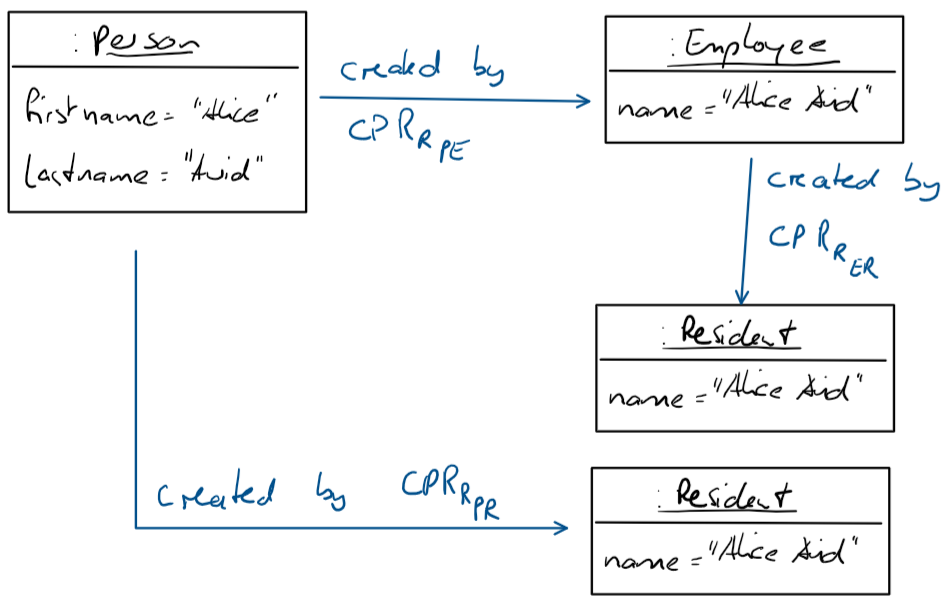
\includegraphics[width=0.8\textwidth]{figures/correctness/synchronization/duplicate_creation_example.png}    
    \caption{Duplicate creation of a resident by two sequences of consistency preservation rules}
    \label{fig:synchronization:duplicate_creation_example}
\end{figure}

An analogous example can be given for the running example of persons, employees and residents depicted in \autoref{fig:networks:three_persons_example}.
We consider the consistency relations $\consistencyrelation{R}{PE}, \consistencyrelation{R}{ER}$ and $\consistencyrelation{R}{PR}$.
As discussed in \autoref{chap:compatibility}, these relations are compatible, thus for any given person, employee or resident, there is a consistent set of models containing it.
Thus, the relations do not prevent transformations from finding consistent models whenever a person, employee or resident is added.
If we now consider ordinary transformations with unidirectional consistency preservation rules, they react to the changes in one model and update another accordingly.
In case of adding a person, this may look as depicted in \autoref{fig:synchronization:duplicate_creation_example}.
For each of the given consistency relations, we assume unidirectional consistency preservation rules that preserve consistency according to them.
They especially create an employee for each added person, and a resident for each created employee and person, respectively.
Since the transformations assume the models to be consistent before applying the changes, they always add a corresponding element when one of the elements is added.
This leads to the situation that both $\consistencypreservationrule{\consistencyrelation{CR}{ER}}$ as well as $\consistencypreservationrule{\consistencyrelation{CR}{PR}}$ create a resident upon creation of a person.
In consequence, there exist two residents with the same name, which does not fulfill the consistency relations.

It is our goal to find out how such a situation can be avoided by proper definition of consistency preservation rules in existing transformation languages.
A simple solution in this example would have been to look for the existence of elements to create first.
This can either be done by using a trace model, which most existing transformation language use to store corresponding elements, or by searching for an appropriate element in the other model.
Using a trace model, however, has some drawbacks and pitfalls, which we will investigate later.

% \begin{copiedFrom}{DocSym}

% % \section{Binary Transformation Interoperability}

% % Multi-model consistency preservation can be a achieved by combining binary transformations to graphs, %of transformations, 
% % with the transformations being executed transitively.
% % Since all binary transformations are developed independently of each other, it is necessary that they interoperate properly in a \emph{non-intrusive} way, thus without the necessity for the developer to understand and modify them, which we refer to as \emph{black-box combination}.

% Even under the assumption that, in contrast to our introductory motivation, all specifications are free of contradictions, it is easy to see that problems arise when combining binary transformations by transitively executing them.
% For example, consider the relations in \autoref{fig:prologue:binary_combination_example}.
% If a component is added to the \ac{ADL}, causing a \ac{UML} class creation due to \ref{fig:prologue:binary_combination_example:R1}, which in turn causes a Java class creation due to \ref{fig:prologue:binary_combination_example:R2}, the transformation for relation \ref{fig:prologue:binary_combination_example:R3} does not know that an appropriate class was already created, if the transformations are treated as black boxes.
% Consequently, the transformation will create the same class again, which may override the existing one, depending on the implementation and execution order.
% A simple solution for this example would be to have all transformations use a common trace model and check for existing elements before creating them in a transformation.
% Nevertheless, independently developed transformations will usually not assume that %this only applies if the transformation considers possibly preexisting transformation results, which it will not do in general if it does not assume other transformations to create corresponding elements.
% other transformations may already have created corresponding elements.
% Additionally, the trace model must allow the transformation engine to retrieve transitive traces.
% However, it is unclear if transitive resolution of traces can always be performed, as it can depend on whether the transitive trace belongs the considered consistency relation or another.
% %If, in another scenario, the transformation in the example was actually supposed to create an additional class, it would have to ignore the existing trace.

% As can be seen in the example, especially the correct handling of trace information in interdependent transformations has to be researched.
% This applies not only to element creations, but also other change types, such as attribute or reference changes, especially if they are multi-valued.
% In our thesis, we will therefore apply transitively executed binary transformations in different case studies to identify these and potential further problems.
% We then want to come up with a catalog of such problems %preventing the black-box combination of transformations 
% together with solution patterns for them.
% For example, to avoid duplicate element creations, a simple pattern could be to always check for already existing traces for that consistency relation in the transformations.
% In consequence, the integration of those patterns into a transformation language or the application of them as a transformation developer is supposed to achieve black-box combinability of the transformations.

% \end{copiedFrom} % DocSym


%%
%% USING FINE-GRAINED RELATIONS
%%
\subsection{Consistency Preservation for Fine-grained Relations}

\mnote{Consistency preservation defined for model-level consistency relations}
In our definition of consistency preservation rules in \autoref{def:consistencypreservationrule}, we used the coarse-grained notion of \modellevelconsistencyrelations, which describe consistency between two models in terms of a single relations.
In consequence, such a \modellevelconsistencypreservationrule ensures consistency to a single consistency relation.

\mnote{Fine-grained consistency relations allow to define relation between unidirectional preservation rules}
In \autoref{chap:compatibility:formal_notion}, we discussed that consistency relations can be considered in a fine-grained way that is able to reflect different notion of consistency in both directions between two models, such as a employee requiring a resident to exist but not vice versa.
We thus refined the notion of consistency relations in \autoref{def:consistencyrelation} to be defined unidirectionally and at the level of model elements rather than complete models.
%This fine-grained notion of consistency does also fit well to how specifications in transformation languages consider consistency, as they define rules that relate only some classes by relations or routines to preserve their consistency.
Since we also consider unidirectional consistency preservation rules as defined in transformation languages, we base further considerations regarding consistency preservation rules on such fine-grained and unidirectional consistency relations.
We later discuss how unidirectional consistency relations and unidirectional consistency preservation rules are related.
Nevertheless, we did also discuss in that chapter that each fine-grained relation can also be translated into a \modellevelconsistencyrelation, thus all insights we already had for those model-level relations still apply to the considerations regarding fine-grained ones.

\mnote{Transformation languages use fine-grained relations and preservation rules}
This fine-grained notion of consistency does also fit well to how specifications in transformation languages consider consistency.
They allow to define rules that relate only some classes by relations, conforming to fine-grained consistency relations, from which then fine-grained consistency preservation rules are derived, or they directly allow to define routines to preserve consistency between specific classes.
These rules are often called \emph{transformation rules} and composed to a transformation that consists of multiple such rules, each encoding a consistency relations and a preservation rule for it.
%We will, however, stick to the coarse-grained notion of consistency preservation rules, because, first, it is difficult to describe how such fine-grained consistency preservation rules can be composed, and second, the coarse-grained notion is sufficient for our considerations anyway.

\mnote{Stick to coarse-grained notion of preservation rules}
It may easily happen that the execution of one transformation rule leads to the violation of the consistency relation of another one, which introduced dependencies between the individual transformation rules.
Thus, a combination of such transformation rules to a transformation has to ensure correctness, i.e., that the consecutive execution of the rules leads to a consistent state of the models.
Languages such as \gls{QVTR} and \gls{QVTO} therefore specify that transformation rules may not be conflicting (cf. \cite[7.10.2.]{qvt}).
It is also a dedicated topic of research to ensure that the rules of a single transformation conform to each other, e.g.\ \cite{cuadrado2017tse,cabot2010jss}, thus we assume that a transformation has that property.
To avoid the necessity of specifying this conformance property for transformation rules, we stick to the existing notion of coarse-grained consistency preservation rules, as it is sufficient for our considerations.

\mnote{New transformation notion based on fine-grained consistency relations}
In consequence, from now we consider a synchronizing transformation as a set of fine-grained consistency relations according to \autoref{def:consistencyrelation} and a consistency preservation rule that preserves consistency according to the set of relations $\consistencyrelationset{CR}$ rather than a single \modellevelconsistencyrelation $\consistencyrelation{CR}{}$.
A consistency preservation rule $\consistencypreservationrule{\consistencyrelationset{CR}}$ and also a transformation with that preservation rule are thus still considered correct if it is applied to a consistent pair of models and changes to them and applying the resulting changes to the models again delivers a pair of models that is consistent to all consistency relations, i.e.:
\begin{align*}
    &
    \forall \model{m}{1} \in \metamodelinstanceset{M}{1}, \model{m}{2} \in \metamodelinstanceset{M}{2}, \change{\metamodel{M}{1}} \in \changeuniverse{\metamodel{M}{1}}, \change{\metamodel{M}{2}} \in \changeuniverse{\metamodel{M}{2}} : \tupled{\model{m}{1},\model{m}{2}} \consistenttomath \consistencyrelationset{CR} \\
    & \formulaskip
    \land \exists \change{\metamodel{M}{1}}' \in \changeuniverse{\metamodel{M}{1}}, \change{\metamodel{M}{2}}' \in \changeuniverse{\metamodel{M}{2}} : \tupled{\change{\metamodel{M}{1}}', \change{\metamodel{M}{2}}'} = \consistencypreservationrule{\consistencyrelationset{CR}}(\model{m}{1}, \model{m}{2}, \change{\metamodel{M}{1}}, \change{\metamodel{M}{2}}) \\
    & \formulaskip\formulaskip
    \Rightarrow \tupled{\change{\metamodel{M}{1}}'(\model{m}{1}),\change{\metamodel{M}{2}}'(\model{m}{2})} \consistenttomath \consistencyrelationset{CR}
\end{align*}
Note that being consistent to all fine-grained consistency relations is equivalent to being consistent to the single \modellevelconsistencyrelation induced by the fine-grained relations.

% In our definition of consistency preservation rules in \autoref{def:consistencypreservationrule}, we used the coarse-grained notion of \modellevelconsistencyrelations and, accordingly, defined \modellevelconsistencypreservationrules that consider models as whole.
% We refined the notion of consistency relations in \autoref{def:consistencyrelation} to be defined at the level of model elements rather than complete models.
% This fine-grained notion of consistency fits well to how specifications in transformation languages consider consistency, as they define rules that relate only some classes by relations or routines to preserve their consistency.
% In the following, we thus also stick to this fine-grained notion of consistency.
% We will, however, stick to the coarse-grained notion of consistency preservation rules given in \autoref{def:consistencypreservationrule}

% \subsection{Feingranulare CPR}
% Jede CPR stellt Konsistenz bzgl. einer unidirektionalen CR wieder her.
% Ein CPR darf keine Änderung machen, die eine andere CR verletzt.
% Schwierig, da CPR voneinander abhängen können (was wiederum dagegen spricht, dass eine CPR nicht eine andere CR verletzen darf), wie also Reihenfolge festlegen?
% Ist keine Option, insbesondere Annahme, dass sich CPR nicht gegenseitig beeinflussen nicht nachvollziehbar (obwohl in der Praxis dasselbe Probleme existiert, da CPR sowieso in feingranulare Regeln zerlegt werden, die natürlich widersprüchlich sein könnten).

%\todo{Relate to the circumstance that we want to consider unidirectional preservation rules, so unidirectional rules might be interesting. We will later find, that this is not the case}


%%
%% UNIDIRECTIONAL CONSISTENCY PRESERVATION RULES
%%
\subsection{Unidirectional Consistency Preservation Rules}

\mnote{Formal definition of unidirectional consistency preservation rules}
Before we can discuss options how unidirectional consistency preservation rules can be used to emulate the behavior of synchronizing consistency preservation rules, we first need to define them to be able to formally compare the two of them.
In contrast to a synchronizing consistency preservation rule as defined in \autoref{def:consistencypreservationrule}, a unidirectional consistency preservation rule does only receive changes made to one of the two models and returns changes to the other models instead of receiving and returning changes to both.

\begin{definition}[Unidirectional Consistency Preservation Rule]
    \label{def:unidirectionalconsistencypreservationrule}
    Let $\metamodel{M}{1}, \metamodel{M}{2}$ be two metamodels and $\consistencyrelationset{CR}$ a set of consistency relations between elements of those metamodels.
    A \emph{unidirectional consistency preservation rule} $\consistencypreservationrule{\consistencyrelationset{CR}}$ for the relation set $\consistencyrelationset{CR}$ is a (usually partial) function:
    \begin{align*}
        \consistencypreservationrule{\consistencyrelationset{CR}} : (\metamodelinstanceset{M}{1}, \metamodelinstanceset{M}{2}, \changeuniverse{\metamodel{M}{1}}) \rightarrow \changeuniverse{\metamodel{M}{2}} \cup \setted{\bot}
    \end{align*}
\end{definition}

\mnote{Preservation rules as defined in or derived from transformation languages}
This is how the consistency preservation rules defined in or derived from existing transformation languages operate.
They take two models and changes to one of them and generate changes for the other.
Most of them even directly apply the changes instead of returning a dedicated change artifact.
If the rule is not able to handle the given changes, it may return $\bot$.

\mnote{Correctness of unidirectional rules analogous to common notions}
In addition, they usually assume the input models to be consistent and then ensure that applying the input and the output changes to the models, the resulting models are consistent again.
This conforms to the common notion of \emph{correctness} for consistency preservation rules, like for the state-based (rather than our delta-based) notion of consistency preservation rules defined in \cite{stevens2010sosym}.
This is even compliant to the correctness notion that we defined for synchronizing consistency preservation rules in \autoref{def:consistencypreservationrulecorrectness}.
Thus, we define correctness of such a unidirectional consistency preservation rule as follows.

\begin{definition}[Unidirectional Consistency Preservation Rule Correctness]
    \label{def:unidirectionalconsistencypreservationrulecorrectness}
    Let $\consistencypreservationrule{\consistencyrelationset{CR}}$ be a unidirectional consistency preservation rule.
    We call $\consistencypreservationrule{\consistencyrelationset{CR}}$ \emph{correct} if the resulting models when applying the generated changes are consistent to $\consistencyrelationset{CR}$ again:
    \begin{align*}
        &
        \forall 
        \model{m}{1} \in \metamodelinstanceset{M}{1}, 
        \model{m}{2} \in \metamodelinstanceset{M}{2},
        \change{\metamodel{M}{1}} \in \changeuniverse{\metamodel{M}{1}} : \\
        & \formulaskip
        \bigl( \tupled{\model{m}{1}, \model{m}{2}} \consistenttomath \consistencyrelationset{CR} \\
        & \formulaskip
        \land \exists 
        \change{\metamodel{M}{2}} \in \changeuniverse{\metamodel{M}{2}} :
        \change{\metamodel{M}{2}} = \consistencypreservationrule{\consistencyrelation{CR}{}}(\model{m}{1}, \model{m}{2}, \change{\metamodel{M}{1}}) \bigr) \\
        & \formulaskip\formulaskip
        \Rightarrow
        \tupled{\change{\metamodel{M}{1}}(\model{m}{1}), \change{\metamodel{M}{2}}(\model{m}{2})} \consistenttomath \consistencyrelationset{CR}
    \end{align*}
\end{definition}

\mnote{Synchronizing consistency preservation rules can be partial}
In \autoref{def:unidirectionalconsistencypreservationrule}, we explicitly allow consistency preservation rules to be partial.
This was only an optional requirement for synchronizing consistency preservation rules defined in \autoref{def:consistencypreservationrule}, because there may be changes to both models which cannot be processed reasonably as one the changes may need to reverted to achieve consistency.
Ignoring that practical requirement, it is theoretically possible to always return changes that, if applied to the input models, produce consistent models.
Those returned changed may perform arbitrarily unreasonable modifications, but still restore consistency.

\mnote{Unidirectinoal consistency preservation rule must be partial}
In general, unidirectional consistency preservation rules need to be partial.
This is due to the reason that there can be models for which no other models can be generated such that they are consistent with respect to a set of consistency relations.
Consider the consistency relations $\consistencyrelation{CR}{} = \setted{\tupled{a, z}, \tupled{b, z}}$ and its transposed $\consistencyrelation{CR}{}^T = \setted{\tupled{z, a}, \tupled{z, b}}$.
If a change generated the model $\model{m}{} = \setted{a, b}$, then no consistent model can be generated.
A consistent model would have to contain $z$, because the consistency relation $\consistencyrelation{CR}{}$ requires for $a$ and $b$ an element $z$ to exist in the other model.
The consistency relation $\consistencyrelation{CR}{}^T$, however, requires that for a $z$ only either $a$ or $b$ exists in the other model, as otherwise no witness structure with unique corresponding elements can be found (see \autoref{def:consistency} for consistency).
In consequence, a unidirectional consistency preservation rule may not produce a result for such an input and thus be partial, as the result would never fulfill the correctness definition.

In fact, the definition does not specify for which inputs a unidirectional consistency preservation rule is allowed to be undefined.
One could restrict this behavior to cases in which there is no $\change{\metamodel{M}{2}} \in \changeuniverse{\metamodel{M}{2}}$ for given models $\model{m}{1}$ and $\model{m}{2}$ as well as change $\change{\metamodel{M}{1}} \in \changeuniverse{\metamodel{M}{1}}$, such that $\tupled{\change{\metamodel{M}{1}}(\model{m}{1}), \change{\metamodel{M}{2}}(\model{m}{2})} \consistenttomath \consistencyrelationset{CR}$ for a set of consistency relation $\consistencyrelationset{CR}$.
We, however, leave it up to the developer to decide for which inputs a consistency preservation rule is undefined, as there might be cases in which a change that restores consistency can be restored, but does semantically not make this.
This was also the reason for allowing a synchronizing consistency preservation rule to be partial, which is why we have already discussed the scenario in \autoref{chap:correctness:formalization:incremental_inductive}.
% \subsection{Partial Definition of Consistency Preservation Rules}
% \todo{Move this to definition of unidirectional preservation rules?}
% 1. Schon eine synchronisierende Transformation muss nicht für jede Eingabe definiert sein. Es könnte natürlich sein, dass sich gleichzeitige Änderungen nicht sinnvoll in Einklang bringen lassen. Theoretisch ist es aber möglich eine total definierte Funktion anzugeben, da immer ein beliebigen (im dümmsten Fall immer dasselbe / leere Modell) zurückgeliefert werden kann.


%%
%% NONALIGNMENT OF UNIDIRECTIONAL CONSISTENCY RELATIONS AND UNIDIRECTIONAL CONSISTENCY PRESERVATION RULES
%%
\subsection{Unidirectional Relations and Preservation Alignment}
\label{chap:synchronization:gap:alignment}

\mnote{Unidirectional consistency preservation rules for each unidirection consistency relation}
Defining unidirectional consistency preservation rules based on a unidirectional notion of consistency relations imposes the idea of having one unidirectional consistency preservation rule associated with one unidirectional consistency relation, or at least a set of unidirectional relations between the same two metamodels.
In consequence, we would have two sets of unidirectional consistency relations between two metamodels and a consistency preservation rule for each of them.

\begin{figure}
    \centering
    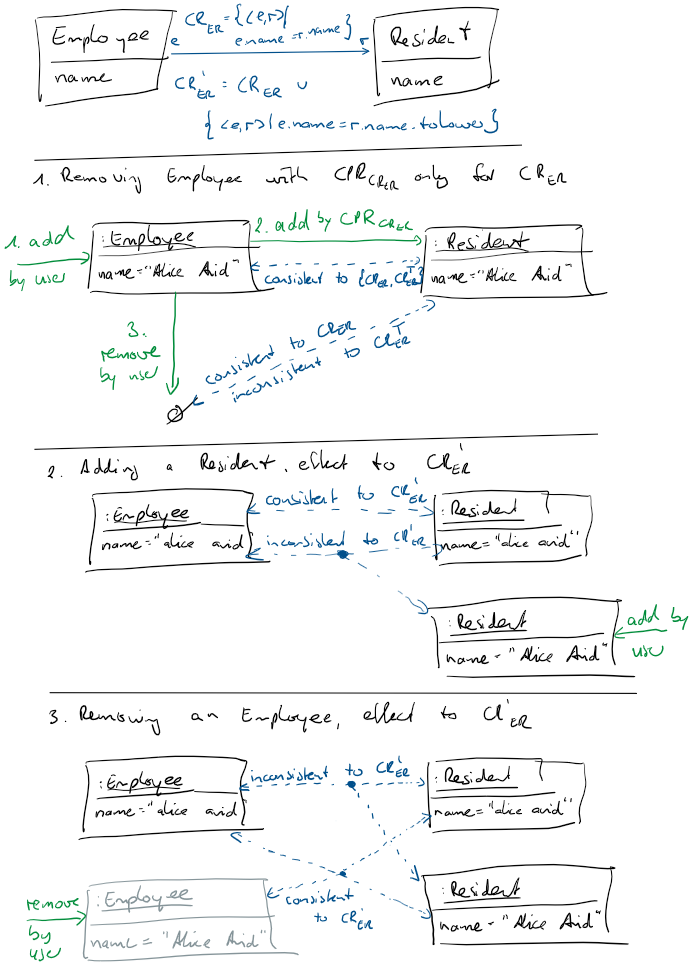
\includegraphics[width=0.9\textwidth]{figures/correctness/synchronization/unidirectional_nonalignment.png}
    \caption[Nonalignment of Unidirectional Relations and Preservation Rules]{Nonalignment of Unidirectional Relations and Preservation Rules. %: scenario for unidirectional consistency preservation rule requiring knowledge about consistency relation in opposite direction (1)
    }
    \todo{Split into two figures}
    \label{fig:synchronization:unidirectional_nonalignment}
\end{figure}

\mnote{Unidirectional consistency preservation rules cannot only consider one direction of consistency relations}
It is, however, easy to see that a unidirectional consistency preservation rule cannot only consider one direction of consistency relations, but needs to consider both.
Consider the example in \autoref{fig:synchronization:unidirectional_nonalignment}, which contains an extract of the consistency relations of the running example.
We assume the consistency relations $\consistencyrelation{CR}{ER}$ and $\consistencyrelation{CR}{ER}^T$ describing that for each employee a single corresponding resident must exist and vice versa.
As discussed before, only considering $\consistencyrelation{CR}{ER}$ would realize the notion of not requiring an employee for every resident.
If we define a unidirectional consistency preservation rule $\consistencypreservationrule{\consistencyrelation{CR}{ER}}$ only for the consistency relation $\consistencyrelation{CR}{ER}$ with the goal to always preserve consistency according to that relation after changes to the employee model, the example scenario 1 in \autoref{fig:synchronization:unidirectional_nonalignment} show that this is not the case.
While for the scenario of adding an employee the rule properly propagates the change by adding a resident and thus restores consistency, removing an employee leads to a violation of consistency.
Removing an employee does not require the consistency preservation rule to perform any changes in the resident model, because $\consistencyrelation{CR}{ER}$ only requires a unique resident to exist for every employee, but does not forbid that there is a resident for which no employee exists.
This is defined by the inverse relation $\consistencyrelation{CR}{ER}^T$.
In consequence, after removing tan employee the consistency preservation rule does not perform any changes, as consistency to $\consistencyrelation{CR}{ER}$ is given, but the model are then inconsistent to $\consistencyrelation{CR}{ER}^T$.

\mnote{Changes to one model may affect consistency relations in both directions}
The given scenario exemplifies the general case that a consistency according to a consistency relation cannot only be violated by performing changes to the model containing the left condition elements of the relations, but also by changes to the model containing the right condition elements of the relation.
In general, consistency of models according to a consistency relation is affected by the presence of condition elements in the models.
Consistency is defined as the ability to find a witness structure, i.e., a unique mapping between condition elements of the consistency relation that occur in the models.
Thus, adding, changing or removing elements in model that constitute a condition element of the consistency relations can lead to inconsistencies.

\mnote{Distinction of addition, removal or change of condition elements for consistency relation affection}
We can see that any type of change can lead to the violation of a consistency relation in either direction:
\begin{properdescription}
    \item[Addition:] Whenever a condition element of the left side of a consistency relation is added to a model, a corresponding condition element need to exist in the other model. If it does not exist yet, the models are not consistent to that relation.
    When a condition element of the right side of a consistency relation is added to a model, this does, according to the definition of consistency, not require another condition element to exist in the other model. It can, however, lead to the situation that no witness structure with a unique mapping between the elements exists anymore.
    Consider the exemplary relation $\consistencyrelation{CR}{ER}'$ in \autoref{fig:synchronization:unidirectional_nonalignment} and the example scenario 2.
    Having an employee with name \enquote{alice avid} and a corresponding resident with the same name, the models are consistent to that relation.
    Adding a resident with name \enquote{Alice Avid} violates $\consistencyrelation{CR}{ER}'$, because the employee \enquote{alice avid} corresponds to both residents, so there is no mapping inducing a witness structure for consistency.
    In consequence, adding a right side condition element of the consistency relation to the models can also violate consistency to a consistency relation.
    \item[Removal:] Whenever a condition element of the right side of a consistency relation is removed from a model, the corresponding condition element in the other model still exists. Because this element does not necessarily have a corresponding one anymore, there may not be a valid witness structure and thus the models may not be consistent anymore.
    When a condition element of the left side of a consistency relation is removed from a model, the originally corresponding element is not connected to the removed element in the witness structure anymore. If another element is considered to this corresponding element, there is no unique mapping of elements anymore.
    Consider again the relation $\consistencyrelation{CR}{ER}'$ in \autoref{fig:synchronization:unidirectional_nonalignment} and the example scenario 3.
    Having two employees and residents with the names \enquote{alice avid} and \enquote{Alice Avid}, the models are consistent because each employee has a corresponding resident and vice versa.
    If we remove the employee \enquote{Alice Avid}, the models are consistent to $\consistencyrelation{CR}{ER}'$ anymore, because the remaining employee corresponds to both residents, so there is no unique mapping of condition elements.
    \item[Change:] We do not have a precise notion of when a condition element can be considered changed, as elements do not have identity. 
    Additionally, consistency in terms of being able to find a witness structure is only based on the existence or non-existence of condition elements, thus whether an element was changed or removed and created makes no different.
    We might say that a condition element can be considered changed when the change describes modifications of the model elements in the condition element that lead to a new condition element within the same condition.
    This does, conceptually, not different from the removal of one and the addition of another condition element.
    Thus, the same situations as discussed for addition and removal above can occur.
\end{properdescription}

\mnote{Unidirectional consistency preservation rules cannot be synchronizing}
%In addition to the insight that unidirectional consistency preservation rule must base on all consistency relations between two metamodels rather than only the ones in a specific direction, 
It is also easy to see that there is no trivial way of specifying a unidirectional synchronizing consistency preservation rule.
It may seem natural to define a consistency preservation rule that is able to process changes in both models and then return only changes in one of them to restore consistency to close the gap between synchronizing and ordinary transformations.
Consider the situation that we have two residents and employees named \enquote{Alice Avid} and \enquote{Bob Do}.
If one of them is removed in the residents model and the other in the employees model, then a proper synchronizing transformation should remove both corresponding elements such that the models are empty.
This requires changes to both models.
With a synchronizing unidirectional consistency preservation rule for each direction, neither of them can produce changes in one of the models that reasonably restore consistency.
Such a rule would necessarily revert one removal to restore consistency, which is not the intended behavior and would probably not be specified by a developer that way, such that the consistency preservation rule would be undefined for that input, although a synchronization transformation would be able to resolve those changes.
In fact, we would expect to have two unidirectional consistency preservation rules of which each removes one of the elements.
This does, however, violate our existing notion of correctness for a single consistency preservation rule.
In the subsequent sections, we will therefore discuss relaxed requirements to unidirectional consistency preservation rules to be able to act like a synchronizing transformations.

% A unidirectional consistency relations require preservation rules in both directions (add/delete)
% \begin{itemize}
%     \item A single unidirectional consistency relation may impose preservation rules in both directions: For each employee, a resident is required, but not every resident needs to be an employee. When then have only one unidirectional consistency relation describing that circumstance. We need, however, consistency preservation rules in both directions, because if, for example, a resident is removed, the employee needs to be removed as well, whereas a resident has to be added whenever an employee is added.
%     \item With ordinary unidirectional rules, we then have that after a change to model 1, the unidirectional rule has to change model 2 so that they are consistent to both unidirectional relations (and vice versa)
% \end{itemize}
% Konsequenz: Wir können nicht für die unidirektionalen Konsistenzrelationen jeweils die CPR in die Richtung angeben, sondern jede unidirektionale CPR muss immer die Konsistenzrelationen in beide Richtungen berücksichtigen.

% Define mapping between change types and directionality of involved consistency relation (delete in opposite direction than add or modification). Make example at witness structures.

% Beachten, dass auch beim Hinzufügen in m2 die Relation m1->m2 verletzt werden kann, da nun zu viele Elemente vorhanden sind -> keine Witness-Struktur.


% \paragraph{Synchronizing Transformation cannot be Unidirectional}
% Es ist einfach zu sehen, dass synchronisierende Transformationen nicht so einfach unidirektional definiert werden können.
% Wird m1 beliebig geändert und in m2 ein Element gelöscht, welches für Konsistenz zu m1 notwendig war, dann kann die unidirektionale CPR m2 nicht wieder so anpassen, dass es konsistent zu m1 ist, außer indem es das gelöschte Element wieder hinzufügt. Hier wäre es richtig das Element in m1 durch die gegenläufige CPR zu löschen. 
% Das bedeutet aber das Korrektheit hier nicht definiert werden kann als die Eigenschaft Konsistenz bzgl. aller CR durch eine unidirektionale CPR herzustellen.

% Das gilt allerdings nur, wenn man den Korrektheitsbegriff beibehält. Wir werden sehen, dass es andere Möglichkeiten gibt diesen Begriff einer unidirektionalen synchronisierenden Transformation zu definieren.


%%
%% COMPOSING TWO UNIDIRECTIONAL CPR TO BIDIRECTIONAL TRANSFORMATIONS
%%
\subsection{Bidirectional Transformations}

\mnote{Unidirectional consistency preservation rules usually appear as pairs}
A unidirectional consistency preservation rule does usually not appear on its own but in combination with another rule for the opposite direction.
We have already seen that even a single unidirectional consistency relation between two metamodels requires unidirectional consistency preservation rules for both directions to preserve consistency according to that relation after changes either instances of either of the metamodels.
In practice, many transformation languages, especially relational ones such as \gls{QVTR} or \gls{TGG} tools, allow the specification of \emph{bidirectional transformations}, which means that they define or derive unidirectional consistency preservation rules for both directions.

\mnote{Combine two unidirectional consistency preservation rules to a bidirectional transformation}
In general, it is reasonable to consider two unidirectional consistency preservation rules between two metamodels together, such that after changes in instances of any of the two metamodels, the other model can be updated to restore consistency.
A synchronizing transformation according to \autoref{def:synchronizingtransformation} is also able to process changes in any of the two models, thus such a notion fits to our goal of emulating synchronizing transformations.
According to common terminology, we define this as a bidirectional transformation.

\begin{definition}[Bidirectional Transformation]
    \label{def:bidirectionaltransformation}
    Let $\metamodel{M}{1}$ and $\metamodel{M}{2}$ be two metamodels and $\consistencyrelationset{CR}$ a set of consistency relations between them.
    Additionally, let $\consistencypreservationrule{\consistencyrelationset{CR},{\rightarrow}}$ and $\consistencypreservationrule{\consistencyrelationset{CR},{\leftarrow}}$ be unidirectional consistency preservation rules with:
    \begin{align*}
        &
        \consistencypreservationrule{\consistencyrelationset{CR}}^{\rightarrow} : (\metamodelinstanceset{M}{1}, \metamodelinstanceset{M}{2}, \changeuniverse{\metamodel{M}{1}}) \rightarrow \changeuniverse{\metamodel{M}{2}} \cup \setted{\bot} \\
        &
        \consistencypreservationrule{\consistencyrelationset{CR}}^{\leftarrow} : (\metamodelinstanceset{M}{2}, \metamodelinstanceset{M}{1}, \changeuniverse{\metamodel{M}{2}}) \rightarrow \changeuniverse{\metamodel{M}{1}} \cup \setted{\bot}
    \end{align*}
    A \emph{bidirectional transformation} is a triple $\transformation{T} = \tupled{\consistencyrelationset{CR},\consistencypreservationrule{\consistencyrelationset{CR}}^{\rightarrow}, \consistencypreservationrule{\consistencyrelationset{CR}}^{\leftarrow}}$.
\end{definition}

\mnote{Correctness of bidirectional transformations}
We call such a bidirectional transformation correct if both consistency preservation rules are correct, i.e., they both preserve consistency according to the underlying consistency relation set.

\begin{definition}[Bidirectional Transformation Correctness]
    \label{def:bidirectionaltransformationcorrectness}
    Let $\transformation{T} = \tupled{\consistencyrelationset{CR}, \consistencypreservationrule{\consistencyrelationset{CR}}^{\rightarrow}, \consistencypreservationrule{\consistencyrelationset{CR}}^{\leftarrow}}$ be a bidirectional transformation.
    We call $\transformation{T}$ correct if, and only if, $\consistencypreservationrule{\consistencyrelationset{CR}}^{\rightarrow}$ and $\consistencypreservationrule{\consistencyrelationset{CR}}^{\leftarrow}$ are both correct according to \autoref{def:unidirectionalconsistencypreservationrulecorrectness}.
\end{definition}

\mnote{Bidirectional transformations do not support changes of both models}
Such bidirectional transformations ensure that if any of two models is changed, a change for the other is generated such that both changed models are consistent again, if possible.
This does, however, not reflect the case that both models have been modified concurrently, as it is the case in transformation networks and thus supported by our initial definition of synchronizing transformations.
We therefore discuss in the following sections how we can combine the unidirectional consistency preservation rules of a bidirectional transformation and which requirements we have to make to them such that the bidirectional transformation behaves like a synchronizing one.


\section{Combining Unidirectional Consistency Preservation Rules}

\mnote{Make bidirectional transformation synchronizing}
We have introduced that bidirectional transformations, as we assume to be the notion for practically usable transformation specifications, can only be applied after changes to one model and update the other to restore consistency.
This induces a gap to synchronizing transformations, as required in transformation networks, which are able to accept changes made in both models and update both models to restore consistency.
To close this gap, we discuss options to combine the unidirectional consistency preservation rules of a bidirectional transformation, such that it considers changes made to both models and thus acts like a synchronizing transformation.


%%
%% OPTIONS TO COMBINE TRANSFORMATIONS / CPRS
%%
\subsection{Options for Combination}
\label{chap:synchronization:combination:options}

\mnote{Conflicting concurrent changes}
Existing work already proposed strategies to synchronize concurrent changes between two models.
This includes techniques for processing concurrent changes with \glspl{TGG}~\cite{hermann2012concurrentSynchronization-FASE,orejas2020IncrementalConcurrentSynchronization-FASE} and specific algorithms for a general notion of synchronizing transformations according to our definition~\cite{xiong2013SynchronizingConcurrentUpdates-SoSym,xiong2009parallelUpdates-ICMT}.
All these approaches, however, deal with the more general case that arbitrary changes may have been made.
This especially includes conflicting updates by one or more users, which need to be resolved and potentially require one of the changes to be reverted.

\mnote{Specific concurrent changes in transformation networks}
We are, however, in the situation that transformations do not perform arbitrary changes and that changes of other transformations may need to be revised but not reverted.
For example, it may be necessary to update an attribute value again, because the interval of consistent values of the currently executed transformation is smaller than the one of a transformation executed before.
It will, however, not be necessary to completely revert the modification of the attribute value, because the modification was necessary for another transformation to restore consistency.
Thus, the causal change for which consistency was restored would need to be reverted as well.
Finally, this would result in reverting a user change, which should never happen.

\mnote{Assumed compatibility of relations}
We assume the consistency relations of transformations to be compatible according to \autoref{def:compatibility}, which excludes contradictions that may prevent transformations from finding a consistent result for specific changes.
This assumptions reduces the potential conflicts that may occur when changes of different transformations need to be synchronized.

\mnote{Execution of both preservation rules}
A bidirectional transformation according to \autoref{def:bidirectionaltransformation} consists of two unidirectional consistency preservation rules.
We have discussed in \autoref{chap:synchronization:gap:alignment} that it is not possible to extend those consistency preservation rules to be synchronizing such that the execution of a single unidirectional consistency preservation rule restores consistency to all consistency relations after changes to both models.
In fact, it will be necessary to execute both preservation rules at least once to restore consistency.
Different options to apply the rules exist, each having individual benefits and drawbacks.

\mnote{Independent execution and merge}
We have sketched two scenarios for executing multiple consistency preservation rules in \autoref{chap:correctness:notions_consistency:preservation}, which can be transferred to the case of executing the two consistency preservation rules of a bidirectional transformation.
A first option is to independently apply the consistency preservation rules and then merge the results.
Imagine models $\model{m}{1}$ and $\model{m}{2}$ and changes $\change{\metamodel{M}{1}}$ and $\change{\metamodel{M}{2}}$ to them.
Applying the two unidirectional consistency preservation rules independently yields $\change{\metamodel{M}{2}}' = \consistencypreservationrule{\consistencyrelationset{CR}}^{\rightarrow}(\model{m}{1},\model{m}{2}, \change{\metamodel{M}{1}})$ and $\change{\metamodel{M}{1}}' = \consistencypreservationrule{\consistencyrelationset{CR}{}}^{\leftarrow}(\model{m}{2}, \model{m}{1}, \change{\metamodel{M}{2}})$.
It is, however, not guaranteed that $\tupled{\change{\metamodel{M}{1}}'(\change{\metamodel{M}{1}}(\model{m}{1})), \change{\metamodel{M}{2}}'(\change{\metamodel{M}{2}}(\model{m}{2}))}$ is consistent to $\consistencyrelationset{CR}$.
It is even not guaranteed that the changes, such as $\change{\metamodel{M}{1}}$ and $\change{\metamodel{M}{1}}'$, can be concatenated at all, since $\change{\metamodel{M}{1}}'$ was generated for $\model{m}{1}$ and not for $\change{\metamodel{M}{1}}(\model{m}{1})$.
As an example, $\change{\metamodel{M}{1}}$ may remove an element from $\model{m}{1}$, which $\change{\metamodel{M}{1}}'$ changes.
Even if the change is still defined for that modified model, the result may not be consistent, because the necessary change produced by $\consistencypreservationrule{\consistencyrelationset{CR}}^{\rightarrow}$ cannot be applied anymore.
Thus merging the changes of both consistency preservation rules does not necessarily yield a consistent result.

\mnote{Sequential execution}
Another option is to sequence the execution.
In a first step, we generate the change $\change{\metamodel{M}{2}}' = \consistencypreservationrule{\consistencyrelationset{CR}}^{\rightarrow}(\model{m}{1},\model{m}{2}, \change{\metamodel{M}{1}})$ as before.
Then, $\tupled{\change{\metamodel{M}{1}}(\model{m}{1}), \change{\metamodel{M}{2}}'(\model{m}{2})}$ is consistent due to correctness of $\consistencypreservationrule{\consistencyrelationset{CR}}^{\rightarrow}$.
Afterwards, we apply the second consistency preservation rule to the newly generated consistent models and the original change $\change{\metamodel{M}{2}}$ to $\model{m}{2}$, thus $\change{\metamodel{M}{1}}' = \consistencypreservationrule{\consistencyrelationset{CR}}^{\leftarrow}(\change{\metamodel{M}{2}}'(\model{m}{2}), \change{\metamodel{M}{1}}(\model{m}{1}), \change{\metamodel{M}{2}})$.
As a result, we receive $\tupled{\change{\metamodel{M}{1}}'(\change{\metamodel{M}{1}}(\model{m}{1})), \change{\metamodel{M}{2}}(\change{\metamodel{M}{2}}'(\model{m}{2}))}$, which is consistent to $\consistencyrelationset{CR}$.
This means that $\change{\metamodel{M}{2}}$ is not applied to $\model{m}{2}$ anymore, in which the changes were performed originally, but needs to be applied to $\change{\metamodel{M}{2}}'(\model{m}{2})$.
It is, again, unclear whether the change can be applied to that state, i.e., whether $\change{\metamodel{M}{2}}$ is defined for $\change{\metamodel{M}{2}}'(\model{m}{2})$.
However, if the changes are applicable, all original changes are reflected in the result.
In addition, the resulting models are consistent because of correctness of the consistency preservation rules.

\mnote{Sequential execution with less drawbacks}
Both discussed options have the drawback that they cannot guarantee to produce a result, as it is possible that the involved changes cannot be concatenated.
In addition, the first option of independently applying the consistency preservation rules and then merging the results cannot even guarantee that the resulting models are consistent if changes can be concatenated.
Thus, we only consider the second option of sequencing the execution of consistency preservation rules and further discuss it in the following.


%%%
%%% SEQUENCING OF CPRS
%%%
\subsection{Sequencing of Consistency Preservation Rules}
\label{chap:synchronization:combination:sequencing}

\begin{figure}
    \centering
    \input{figures/correctness/synchronization/sequencing_schema.tex}
    %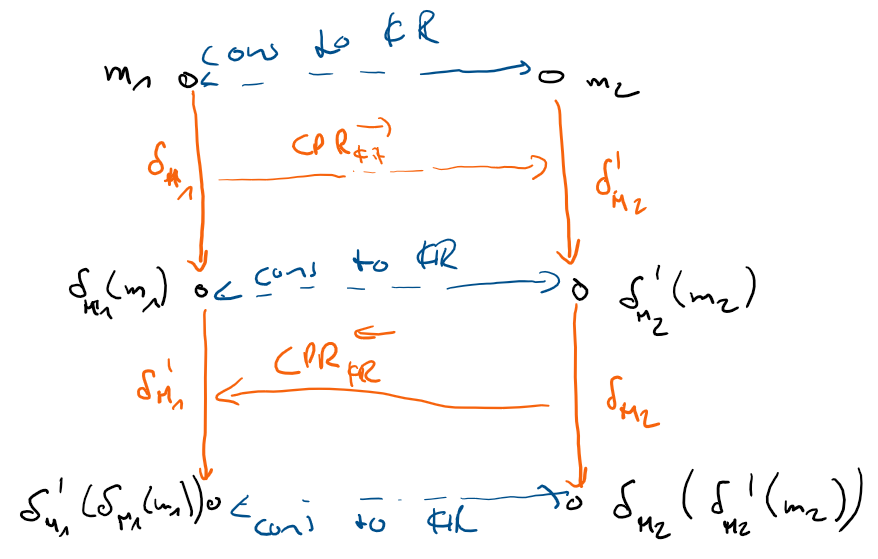
\includegraphics[width=0.8\textwidth]{figures/correctness/synchronization/sequencing_schema.png}
    \caption[Sequencing unidirectional consistency preservation rules]{Schema for sequencing unidirectional consistency preservation rules after concurrent changes. Circles denote model states, blue lines connect consistent models, and green lines with arrowheads denote the execution of changes or consistency preservation.}
    \label{fig:synchronization:sequencing_schema}
\end{figure}

\mnote{Changes affecting disjoint element sets}
The sequential application of original changes and execution of consistency preservation rules is depicted schematically in \autoref{fig:synchronization:sequencing_schema}.
It has two important properties. 
First, it ensures that all original changes are applied to the models and, second, it guarantees that the resulting models are consistent.
It is, however, only applicable in specific situations.
The optimal case, in which the approach is always applicable, is if $\consistencypreservationrule{\consistencyrelationset{CR}}^{\rightarrow}$ produces changes for the second model that affect a disjoint set of elements in $\consistencyrelationset{CR}$ compared to the original changes to the second model $\change{\metamodel{M}{2}}$.
If two changes affect completely disjoint sets of elements, they can obviously be consecutively applied.
It would then not even make a difference in which order they are applied.

\begin{figure}
    \centering
    \input{figures/correctness/synchronization/non_transformability.tex}
    %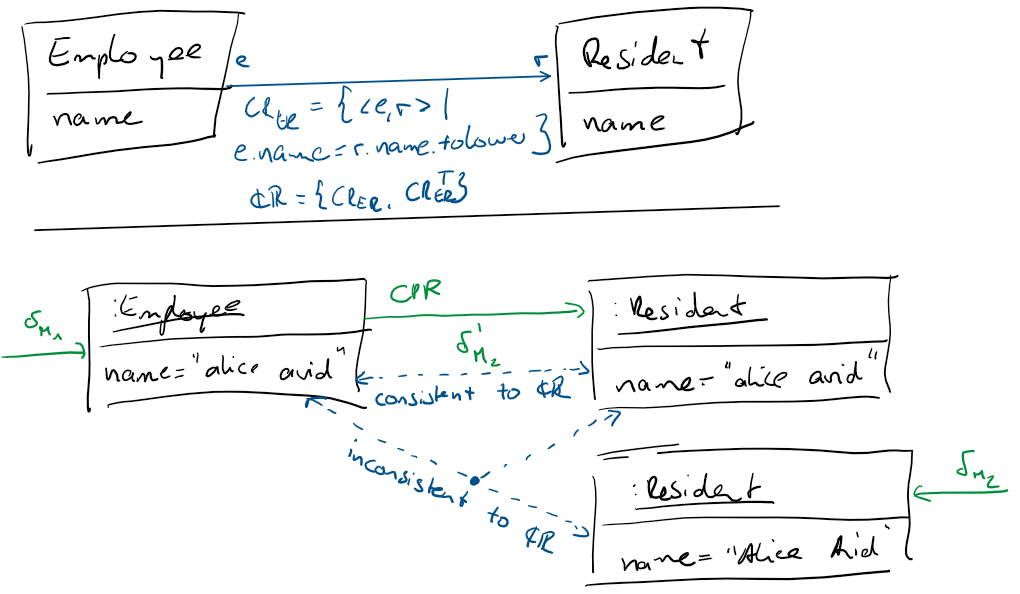
\includegraphics[width=0.9\textwidth]{figures/correctness/synchronization/non_transformability.png}
    \caption[Non-transformability in sequencing scenario]{Example for non-transformability when sequencing the application of unidirectional consistency preservation rules and concurrent changes.
    Blue lines without arrowheads connect elements that are \mbox{(in-)}consistent to $\consistencyrelationset{CR}$, and green lines with arrowheads indicate changes.}
    \label{fig:synchronization:non_transformability}
\end{figure}

\mnote{Issues when sequencing preservation rule application}
Unfortunately, the change $\change{\metamodel{M}{2}}'$ produced by $\consistencypreservationrule{\consistencyrelationset{CR}}^{\rightarrow}$ and the original one $\change{\metamodel{M}{2}}$ produced by other transformations do not necessarily affect disjoint sets of elements.
In that case, the two following problems can occur.
\begin{properdescription}
    \item[Non-Applicability:] The most obvious problem, which we have already discussed, is that the original change to the second model $\change{\metamodel{M}{2}}$ cannot be applied to the model changed by $\change{\metamodel{M}{2}}'$ as the result of $\consistencypreservationrule{\consistencyrelationset{CR}}^{\rightarrow}$. 
    This can, for example, happen when $\change{\metamodel{M}{2}}'$ removes an element that is affected by $\change{\metamodel{M}{2}}$.
    Since the element was changed in $\change{\metamodel{M}{2}}$, it is part of a condition element in another transformation that was executed before.
    As $\consistencypreservationrule{\consistencyrelationset{CR}}^{\rightarrow}$ removed that element, the condition element does no longer exist anyway, thus this removal has to be propagated back by the transformation that originally introduced the change $\change{\metamodel{M}{2}}$.
    In consequence, the modification in $\change{\metamodel{M}{2}}$ can simply be ignored.
    In the worst case, all elements affected by $\change{\metamodel{M}{2}}$ were removed by $\change{\metamodel{M}{2}}'$.
    Then, $\change{\metamodel{M}{2}}$ can be completely ignored, because all condition elements of the involved consistency relations were removed.
    Thus, we can always ensure that the changes, at least those that are still relevant, can still be applied.
    
    \item[Non-Transformability:] Even if the change $\change{\metamodel{M}{2}}$ can be applied to $\change{\metamodel{M}{2}}'(\model{m}{2})$, this does not guarantee that $\consistencypreservationrule{\consistencyrelationset{CR}}^{\leftarrow}$ is able to process the given change.
    In fact, this requirement applies to all changes, even including original user changes, but there are special circumstances in this situation that make the transformation prone to not being able to transform the changes.
    Whenever $\change{\metamodel{M}{2}}'$ adds condition elements that were already added by $\change{\metamodel{M}{2}}$, their concatenation can lead to a duplication of those elements.
    Consider the scenario depicted in \autoref{fig:synchronization:non_transformability} with consistency relations $\consistencyrelationset{CR} = \setted{\consistencyrelation{CR}{ER}, \consistencyrelation{CR}{ER}^T}$. 
    An employee \enquote{alice} is added by the original change to $\model{m}{1}$.
    The consistency preservation rule then generates an appropriate resident with the same name to fulfill the consistency relation.
    The original change to $\model{m}{2}$ adds a resident \enquote{Alice}, which was generated by another transformation, e.g., the one that created an appropriate person and changed the capitalization of the name.
    Applying this original change leads to two residents with different name capitalizations.
    Now it is impossible for $\consistencypreservationrule{\consistencyrelationset{CR}}^{\leftarrow}$ to generate a change $\change{\metamodel{M}{1}}'$ for the first model to restore consistency. The employee corresponds to both residents, as both fulfill the constraint of the consistency relation. 
    But there is no additional employee that could be added to achieve a unique mapping between corresponding elements.
    A synchronizing transformation would have been able to produce a consistent result by considering both original changes at once and then simply not performing any additional changes, as the originally added resident is already consistent to the originally added employee.
    In consequence, if the unidirectional consistency preservation rule had known that the resident was already added, it would not have performed any changes.
\end{properdescription}

\mnote{Non-transformable changes of users unavoidable}
As remarked before, the situation that certain changes cannot be processed by the consistency preservation rules cannot be avoided. 
If the user had added the second resident in the previous scenario, there would have also been no possibility for the consistency preservation rule to generate changes that restore consistency.
The difference is, however, that in this case it is fine that no result is found.
In case of the scenario discussed above, the original changes could have been reasonably processed to a consistent result if the unidirectional consistency preservation rule would have considered that there was already a change that restored consistency.

\mnote{Necessity to process inconsistent inputs}
In consequence, it is inevitable that consistency preservation rules need to be able to deal with the situation that the target model was already modified, such that the given models are not initially consistent.
This is necessary to reflect the changes that have already been made and to integrate them into consistency preservation.
In consequence, we finally have to relax our requirements for the input of consistency preservation rules to be able to consider the changes to both models.
This means that we need to make further requirements to the preservation rules, because we do not yet assume the consistency preservation rules to produce results for inputs that are not consistent.
We have already given examples for scenarios in which it is not possible to restore consistency by one unidirectional consistency preservation rule after changes in both models.

\mnote{Relaxed notion affecting number of executions}
Before we define a precise notion of further requirements to consistency preservation rules that accept inconsistent inputs, we first discuss how often it may be necessary to execute both consistency preservation rules to restore consistency, as this directly affects the requirements we have to define.


%%%
%%% NON-TERMINATION
%%%
\subsection{Execution Bounds}
\label{chap:synchronization:combination:bounds}

\mnote{Unidirectional preservation rules cannot always be correct}
Correctness of unidirectional consistency preservation rules ensures that after executing such a rule the resulting models are consistent.
It is easy to see that this correctness notion cannot be fulfilled for certain sets of consistency relation sets.
This is exemplified at the artificial scenario depicted in \autoref{fig:synchronization:multiple_unidirectional_execution}.
We consider two consistency relations $\consistencyrelation{CR}{1}$ and $\consistencyrelation{CR}{2}$ and their transposed relations, i.e., $\consistencyrelationset{CR} = \setted{\consistencyrelation{CR}{1}, \consistencyrelation{CR}{1}^T, \consistencyrelation{CR}{2}, \consistencyrelation{CR}{2}^T}$.
$\consistencyrelation{CR}{1}$ requires that for each \modelelement{A} an instance of \modelelement{B} exists that has the same value of $i$ incremented by $1$.
The only exception is that if $i$ in \modelelement{A} is $4$ (or any other arbitrary value), then no corresponding element \modelelement{B} is required.
$\consistencyrelation{CR}{2}$ requires that for each \modelelement{A} an instance of \modelelement{B} exists, which has the same value of $i$.
We want to define a bidirectional transformation of two unidirectional consistency preservation rules $\consistencypreservationrule{\consistencyrelationset{CR}}^{\rightarrow}$ for propagating changes in models with instances of \modelelement{A} to one with instances of \modelelement{B} and $\consistencypreservationrule{\consistencyrelationset{CR}}^{\leftarrow}$ to propagate changes in the opposite direction. 

\begin{figure}
    \centering
    \input{figures/correctness/synchronization/multiple_unidirectional_execution.tex}
    %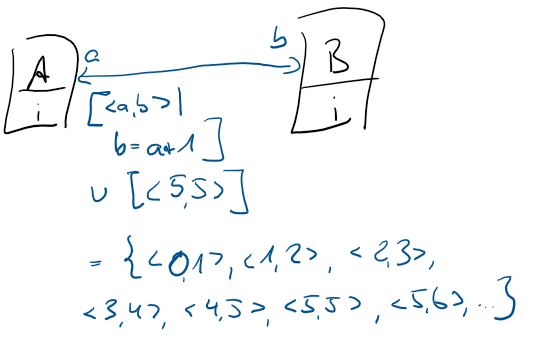
\includegraphics[width=0.7\textwidth]{figures/correctness/synchronization/multiple_unidirectional_execution.png}
    \caption[Multiple execution of consistency preservation rules]{Two consistency relations requiring multiple executions of unidirectional consistency preservation rules to find a consistent result.}
    \label{fig:synchronization:multiple_unidirectional_execution}
\end{figure}

\mnote{Example scenario}
Consider the following scenario: If an \modelelement{A} with $i = 0$ is added to an empty model, $\consistencypreservationrule{\consistencyrelationset{CR}}^{\rightarrow}$ cannot perform any changes in an (also empty) model with instances of \modelelement{B} that restore consistency.
Because of $\consistencyrelation{CR}{1}$, a \modelelement{B} with $i = 1$ has to be created, and because of $\consistencyrelation{CR}{2}$, a \modelelement{B} with $i = 0$ has to be created.
While this also fulfills $\consistencyrelation{CR}{1}^T$, the existence of \modelelement{B} with $i = 1$ requires the existence of an \modelelement{A} with $i = 1$ due to $\consistencyrelation{CR}{2}^T$.
Since $\consistencypreservationrule{\consistencyrelationset{CR}}^{\rightarrow}$ cannot modify the model with instances of \modelelement{A}, it is impossible for $\consistencypreservationrule{\consistencyrelationset{CR}}^{\rightarrow}$ to restore consistency in that case.

\mnote{Multiple executions leading to consistent result}
Allowing the consistency preservation rules to react to each other multiple times can, however, lead to a consistent result.
If $\consistencypreservationrule{\consistencyrelationset{CR}}^{\leftarrow}$ adds an \modelelement{A} with $i = 1$ in response to the previous execution of $\consistencypreservationrule{\consistencyrelationset{CR}}^{\rightarrow}$, all consistency relations except $\consistencyrelation{CR}{1}$ are fulfilled.
$\consistencypreservationrule{\consistencyrelationset{CR}}^{\rightarrow}$ can then create a \modelelement{B} with $i = 2$, which is iteratively processed by $\consistencypreservationrule{\consistencyrelationset{CR}}^{\leftarrow}$.
This process terminates as soon as $\consistencypreservationrule{\consistencyrelationset{CR}}^{\leftarrow}$ adds an \modelelement{A} with $i = 4$, as then $\consistencyrelation{CR}{1}$ is also fulfilled, because it does not require a corresponding \modelelement{B} for an \modelelement{A} with $i = 4$.

\mnote{Arbitrary high number of necessary executions}
We have seen that it is possible to execute unidirectional consistency preservation rules multiple times to achieve a consistent state and that it is not always possible to ensure consistency with only one execution of such a rule.
In fact, the number of necessary executions of consistency preservation rules can be arbitrarily high.
The value of $5$ in $\consistencyrelation{CR}{1}$ of the example can be exchanged by any value requiring an arbitrary high number of executions.
We may only circumvent this by requiring that $\consistencypreservationrule{\consistencyrelationset{CR}}^{\rightarrow}$ must perform changes such that $\consistencypreservationrule{\consistencyrelationset{CR}}^{\leftarrow}$ can then restore consistency with a single execution.
In our scenario, this would mean that $\consistencypreservationrule{\consistencyrelationset{CR}}^{\rightarrow}$ adds all instances of \modelelement{B} with $i \leq 4$.
Anyway, such a behavior requires a relaxation of the correctness requirement for consistency preservation rules, because the execution of $\consistencypreservationrule{\consistencyrelationset{CR}}^{\rightarrow}$ can never result in a consistent state.

\mnote{Preservation rules complete partial condition elements}
Additionally, it may be desired that elements of a consistency relation are created by a consistency preservation rule, although a condition element was only created partially so far.
In that case, the partial condition element has to be completed in one model in addition to the creation of the corresponding condition element in the other model.
Thus, changes in both models are required, which can only be achieved by executing both consistency preservation rules and accepting that executing the first one does not result in consistent models.
An example for such a scenario could be the consistency relation between a component in the \gls{PCM} and its realization as a package and a class in Java.
It may be desired that a package at a specific place, e.g., within a \enquote{components} package, or with a specific name, e.g., containing \enquote{Component}, in the Java code is identified as a component.
Creating such a package shall then lead to the creation of a component in the the \gls{PCM} model as well as of the implementation class in Java.
In that case, there is no complete condition element created in Java, because this would also require the existence of an appropriate class.
If the elements shall still be created, both models have to be changed.
Thus, the first consistency preservation rule introduces the \gls{PCM} component, which introduces an inconsistency between the models, as the corresponding Java class is missing.
This is then corrected by the consistency preservation rule in opposite direction adding the implementation class.

\mnote{Necessity of termination guarantee}
Finally, it is questionable whether such scenarios should be considered in the formal framework or if it should be up to a developer to implement such a scenario without having specific guarantees regarding termination of the consistency preservation rules or regarding consistency of the models after executing the rules a specific number of times.
Since we need to relax the requirement of consistency preservation rules to always produce consistent results after one execution in the synchronization scenario where both models have been modified, we will allow the consistency preservation rules to be executed more than once anyway.
Regarding the example in \autoref{fig:synchronization:multiple_unidirectional_execution}, if we started with an \modelelement{A} with $i = 6$ and let the consistency preservation rules operate as discussed above, i.e., always adding the elements with $i$ incremented by one, this process would never terminate.
We thus need to ensure that such an execution terminates.
Since the consistency preservation rules depend on each other, this will, however, be a property of the bidirectional transformation rather than the individual consistency preservation rule.


\subsection{Necessity for Synchronization Extension}

\mnote{Processing inconsistent input models}
In the previous subsections, we have discussed that after changes to two models, these changes and the ones produced by consistency preservation rules that restore consistency between these models cannot be sequenced in a way such that we receive consistent models in all cases the consistency preservation rules are able to handle.
We especially found that it is necessary for a unidirectional consistency preservation rule to consider the changes made to the model it is supposed to modify.
Thus, we need to enable consistency preservation rules to deal with the situation that the input models are inconsistent.
In our current definition, no behavior of a consistency preservation rule and the encapsulating bidirectional transformation for such a situation is defined.
Thus, we discuss an appropriate extension of bidirectional transformations that support this scenario of synchronization in the following section.

\mnote{Guaranteeing termination}
Additionally, we found that consistency preservation rules may need to be executed multiple times.
This is obviously necessary to make bidirectional transformations synchronizing, as they need to be able to change both models after both of them may have been modified.
Therefore, we consider how we can achieve execution bounds, such that the termination of multiple executions of the consistency preservation rules of a bidirectional transformation is guaranteed.



%%%%
%%%% VERSCHIEDENE VERSUCHE FÜR STRATEGIEN ZUR KOMBINATION VON CPRS
%%%%

% \subsection{Consideration at Condition Element Level}
% % CONSIDERATIONS DO NOT WORK PROPERLY
% \begin{itemize}
%     \item Unidirectional synchronizing: correct if applied to changes d1 to m1, but produces changes d2' that can be applied to d2(m2) as well, and vice versa produces changes d1' for changes d2 to model m2 that can be applied to d1(m1) as well. (Property: Sequentializability, produced changes can handle arbitrary other changes added before)
%     \item For each condition element in d1(m1), i.e., each element for which a consistency relation applies, and for each condition element in d2'(m2), we find exactly one corresponding element in the other model (this is what correctness means). Additionally, in d2'(d2(m2)) $\cap$ d2'(m2), i.e., those elements that are not affected by d2, we also find corresponding 
    
%     \item Take all condition elements in m1 and m2. Take all those for which still only one corresponding condition element exists between m1 and d2(m2), i.e., all the ones not affected by d2. For all of them present in d1(m1) and d2'(d2(m2)), there is still exactly one corresponding condition element. For the ones in d1(m1), which were not in m1, there is a corresponding element in d2'(d2(m2)) and for the ones in d2'(m2), which are also present in d2'(d2(m2)), there is one in d1(m1).
%     \item What if d2'(d2(m2)) produces a new condition element that was not present in m2 and d2(m2) and d2'(m2)? We need to show that this cannot occur?
%     \item Non-synchronizing: d1 and d2 may induce violations of consistency relations. d1' and d2' restore fulfillment of these consistency relations. We consider how consistency relations can be violated when we put d2 in front of d2' and d1 in front of d1' other than in the case when its applied directly.
% \end{itemize}


% \subsection{Versuch über ursächliche Condition Element Änderungen zu unterscheiden}
% Fälle:
% 1. Condition Element wird neu erzeugt
% 2. Condition Element wird geändert, sodass nun ein anderes Element der gleichen Condition vorhanden ist
% 3. Condition Element wird gelöscht
% Es können bei einem Change mehrere davon bzgl. verschiedener Conditions auftreten (also bzgl. verschiedene Consistency Relations)

% Fall 1: Die Vereinigung der Condition Elements aus d2(m2) und d2'(m2) ist gleich derer in d2'(d2(m2)). Somit wird durch die Kombination kein neues Condition Element eingeführt, für das Konsistenz hergestellt werden müsste.

% Fall 2: Die Vereinigung der Condition Elements aus d2(m2) und d2'(m2) ist ungleich derer in d2'(d2(m2)). Somit wird durch die Kombination ein neues Condition Element eingeführt, für das Konsistenz hergestellt werden müsste.

% NEUE STORY:

% Allgemeine Betrachtung von Änderungen: Es geht immer darum, dass Condition Elemente geändert/gelöscht/hinzugefügt wurden und die CPR entsprechend reagieren muss, um das Vorhandensein einer entsprechenden Witness-Struktur zu garantieren. Dabei können entsprechend folgende Fälle auftreten:
% 1. Änderungen führen dazu, dass ein neues Condition Element im Modell existiert, dass zuvor nicht vorhanden war.
% 2. Änderungen führen dazu, dass Elemente eines bereits vorhandenes Condition Elementes geändert werden und dadurch ein andere Condition Element derselben Condition instanziieren.
% 3. Änderungen führen dazu, dass ein vorher existierendes Condition Element nicht mehr im Modell auftaucht.

% Es gibt hierzu drei entsprechende Reaktionen der CPR:
% 1. Im anderen Modell werden, falls nicht vorhanden, entsprechende Elemente erzeugt, um für das neue Condition Element ein eindeutiges korrespondierendes Condition Element zu erzeugen und somit eine Witness-Struktur aufzubauen. (Erzeugungs-Propagation)
% 2. Das gem. Witness-Struktur korrespondierende Condition Element im anderen Modell wird so angepasst, dass wieder eine valide Witness-Struktur entsteht. (Änderungs-Propagation)
% 3. In dem anderen Modell werden die Elemente des korrespondierenden Condition Elementes entfernt (oder zumindest Teile davon), sodass entsprechend der Konsistenzregeln keine weiteren Elemente vorhanden sein müssen, d.h. wieder eine valide Witness-Struktur vorhanden ist.

% % DIE FOLGENDEN ZWEI PARAGRAPHEN SIND NUN BEI DER STRIKTEN SEQUENTIALISIERUNG
% Wenn wir die unidirektionalen CPR sequentialisieren (also erst d2' erzeugen, dann d2 darauf anwenden), kann es sein, dass d2'(m2) Änderungen an Condition Elements in m2 vornimmt oder neue hinzufügt, um Konsistenz wiederherzustellen, die ebenfalls von d2 eingefügt werden, sodass es nicht mehr möglich ist, durch die rückwärtige CPR Änderungen vorzunehmen, die eine valide Witness-Struktur induzieren.
% Z.B. könnte d2'(m2) einen Resident hinzufügen, der bereits durch d2 eingefügt wurde (weil er über einen andere Pfad erstellt wurde, siehe \autoref{fig:synchronization:duplicate_creation_example}). Wird nun d2 auf d2'(m2) angewendet, würde ggf. in einem Container, in dem die Residents gespeichert werden, zwei Residents mit gleichem Namen eingefügt. Für diese kann aber keine Änderung in m1 (sei es das Employee-Modell) erzeugt werden, durch die eine valide Witness-Struktur entsteht. Das Einfügen eines zweiten Employee mit dem gleichen Namen führt dazu, dass jeder Employee und jeder Resident zu zwei Residents bzw. Employees korrespondiert, was keine eindeutige Witness-Struktur induziert.
% Um dies zu vermeiden, müssen die CPR sicherstellen, dass in den Änderungen am anderen Modell nicht bereits entsprechende Condition Elements erzeugt wurden.
% Alle anderen Änderungen sind unproblematisch, da Änderungen die d2 an bestehenden Condition Elements, die nicht zu neuen Condition Elements führen, durchführt mittels 2->1 propagiert werden können, indem die Condition Elements in m1 angepasst werden.

% Insgesamt ist die Situation die gleiche, als würde ein Nutzer eine entsprechende Änderung machen. Auch er kann natürlich einen zweiten Resident mit demselben Namen einführen. Hier würde die CPR selbstverständlich fehlschlagen. Während das für Nutzeränderungen erwünscht ist, da die doppelte Erzeugung desselben Elementes hier schon vom Nutzer durchgeführt wurde und für einen entsprechende Nutzeränderung kein konsistentes Modell generiert werden kann, ist dies innerhalb des Transformationsnetwerkes unerwünscht, da die CPR natürlich eine konsistente Modellmenge finden können und die doppelte Erzeugung lediglich daher kommt, dass die Transformationen nicht, wie verlangt, synchronisieren sind. In letztem Fall wäre sichergestellt, dass nach entsprechenden Änderungen an beiden Modellen (also Erzeugung von Employee in einem, Erzeugung des passenden Resident im anderen) keine Änderungen gemacht werden, da bereits eine passende Witness-Struktur vorhanden ist.
% Die unidirektionalen CPR schaffen das jedoch nicht, da Ihnen die entsprechende Information fehlt.


% \subsection{Erster Versuch zur Partiellen Konsistenz}
% % DIE FOLGENDEN PARAGRAPHEN SIND IN DER PARTIELLEN KONSISTENZ AUFGEGANGEN, NUR DAS PARTIELLE KONSISTENZ ÜBER MODELLE UND NICHT ÜBER CPR DEFINIERT IST
% Was kann nun passieren, wenn wir die CPR mit dem modifizierten Ziel-Modell aufrufen?
% Wir müssen Def anpassen, da es nun nicht mehr reicht, wenn CPR für konsistente Eingabe korrekt ist.

% m1 und d2(m2) sind ja immer noch partiell konsistent. Wir betrachten für jedes Konsistenzrelation alle condition elements in m1 und d2(m2).
% Diejenigen, für die es ein eindeutiges korrespondierendes Element gibt, also eine maximale Menge (es gibt keine Menge, von der sie eine Teilmenge ist) für die es eine Witness-Struktur gibt, und die immer noch in d1(m1) bzw. d2'(d2(m2)) vorkommen, muss es auch darin ein eindeutiges korrespondierendes Element geben.
% Außerdem muss für alle Condition Elements in d1(m1) $\setminus$ m1 und in d2'(d2(m2)) $\setminus$ d2(m2) ein eindeutiges korrespondierendes Element existieren.
% Dies ist bereits dadurch sichergestellt, dass ja die CPR immer auf das Erzeugen/Ändern/Löschen eines Condition Elementes reagieren, d.h. für die Element ein d1(m1) $\setminus$ m1 stellt es Konsistenz sicher und für d2'(d2(m2)) auch, da es sonst eine neue Inkonsistenz induzieren würde.
% D.h. nur für Elemente, die vorher nicht konsistent waren, ist keine Konsistenz verlangt.

% Property: Always-preserving
% CPR erhält Konsistenz für solche Elemente, die vorher konsistent waren. D.h. wenn es eine Witness-Struktur für eine Teilmenge der Modelle gibt, dann gibt es sie auch nach den Änderungen (also in d1(m1) und d2'(d2(m2))) für dieselben Teilmengen (bzw. das was noch davon da ist), egal ob die Modelle vorher konsistent waren oder nicht. (es ist schwer diese Eigenschaft für Transformationen zu zeigen, aber die empirische Evaluation zeigt, dass die Annahme dort zumindest gilt)

% Property: Delta-Correcting
% CPR stellt Konsistenz für solche Elemente her, die durch das Delta im Quellmodell und Zielmodell hinzugefügt werden. Also für alle Condition Elements in d1(m1) $\setminus$ m1 und in d2'(d2(m2)) $\setminus$ d2(m2) muss ein eindeutiges korrespondierendes Element existieren.

% \subsection{Zweiter Ansatz zur partiellen Konsistenz auf Condition Element Level}
% Wir fordert für alle Condition Elements in d1(m1) und alle in m1, die noch immer in d1(m1) vorkommen, dass sie wieder ein eindeutiges korrespondierendes in d2'(d2(m2)) haben, wenn sie in m1 vorhanden waren und dort ein korrespondierendes in d2(m2) hatten.
% Fallunterscheidung:
% * Sie waren in m1 vorhanden, aber in d1(m1) nicht mehr: Dann wurden sie geändert. Wurde das korrespondierende Element in d2(m2) nicht gegenüber m2 geändert, muss es mit d2'(d2(m2)) von CPRr angepasst werden, da sonst auch ohne d2(m2) CPRr die Änderung nicht vorgenommen hätte und damit nicht korrekt wäre. Wurde das Element in d2(m2) gegenüber m2 geändert, so kümmert sich CPRl noch um diese Änderung. \todo{Das können wir nicht transitiv so machen}
% * \dots


% \subsection{Co-occurring Changes to Corresponding Elements}
% Two problem cases: 
% 1. Both d1 and d2 affect corresponding condition elements (otherwise show that it is unproblematic); 
% 2. d2'(d2(m2)) introduced new condition elements that were neither present in m2, nor in d2'(m2), nor d2(m2), so they are neither consistent due to correctness of forward preservation rule, nor processed by backward preservation rule.
% \begin{itemize}
%     \item If d1 affects a condition element (be it a change of an existing, the creation of a new one or the removal of an old one), then preservation needs to generate a d2' that updates/creates/removes the corresponding condition elements appropriately, such that even elements that are potentially part of another condition element, fulfill consistency (due to correctness). If d2 does not affect any of the corresponding or other changes elements, everything is fine, because then we can simply sequence changes.
%     \item 
% \end{itemize}
    
% Szenarien:
% Auf jeder Seite wurde ein Condition Element modifiziert.
% 1. 1->2 und 2->1 ändern jeweils Elemente aus komplett disjunkten Condition Elements: Witness-Struktur ergibt sich aus alter Witness-Struktur und für entfernen von Element und korrespondierendem das Entfernen der Korrespondenz, Hinzufügen und Element und korrespondierendem das Hinzufügen der Korrespondenz, sowie Ändern eines Condition Elementes zu einem anderen das Ändern der entsprechenden Korrespondenz.
% 2. 1->2 (resp.~2->1) fügen durch Änderungen neues Condition Element ein: Sind per Korrektheit verpflichtet das richtig aufzulösen
% 3. \dots

\section{Synchronizing Bidirectional Transformations}

\mnote{Extend consistency preservation rules to accept models that are not consistent}
In the following, we discuss how we can extend bidirectional transformations and especially their unidirectional consistency preservation rules such that they are able to deal with the situation that both models may have been modified.
To achieve this, we extend consistency preservation rules such that they also accept models that are not initially consistent.
We can then not require them to restore consistency between the models with a single execution anymore.
Instead, we define a notion of \emph{partial consistency}, which allows us to specify how the execution of consistency preservation rules has to improve partial consistency.
We derive requirements to the transformations and finally show that transformations fulfilling these requirements terminate consistently.


\subsection{Partial Consistency of Models}

\mnote{Changed models still fulfill some kind of partial consistency notion}
Given two models $\model{m}{1}$ and $\model{m}{2}$ and changes $\change{\metamodel{M}{1}}$ and $\change{\metamodel{M}{2}}$ to each of them, a unidirectional consistency preservation rule $\consistencypreservationrule{\consistencyrelationset{CR}}^{\rightarrow}$ needs to accept and process the change in one model, be it $\change{\metamodel{M}{1}}$ without loss of generality, and receive the unchanged model $\model{m}{1}$ as well as the changed second model $\change{\metamodel{M}{2}}(\model{m}{2})$.
We discussed the necessity to process the changed second model in the previous section.
Whereas $\model{m}{1}$ and $\model{m}{2}$ are consistent, $\model{m}{1}$ and $\change{\metamodel{M}{2}}(\model{m}{2})$ may not.
In consequence, $\consistencypreservationrule{\consistencyrelationset{CR}}^{\rightarrow}$, even if correct according to \autoref{def:unidirectionalconsistencypreservationrulecorrectness}, cannot guarantee that applying the delivered change delivers consistent models.
$\model{m}{1}$ and $\change{\metamodel{M}{2}}(\model{m}{2})$ will, however, usually still fulfill some kind of partial consistency notion.
Depending on the complexity of $\change{\metamodel{M}{2}}$ large parts of the models will still fulfill some kind of consistency notion.

\mnote{Two options to define partial consistency}
Such a notion of partial consistency may be defined in two different ways.
First, we may say that two models only fulfill the consistency relations partially.
Second, we may say that only extracts of two models fulfill the consistency relations.

\mnote{Partial consistency as fulfilling subsets of consistency relations}
In the first option, we consider that the given models are only consistent to a subset of the given consistency relations.
There may, however, be only a single element in the models that leads to the violation of all consistency relations.
Thus, we would call the models completely inconsistent just because of a single element.
To circumvent hat, we would need to define a notion of partial consistency relations, which allows us to define that models are consistent to parts of consistency relations.
Such a notion would have to be defined at the level of consistency relation pairs and their condition elements within the consistency relations.
It would, however, not make sense to consider subsets of consistency relations, i.e., only a subset of their consistency relation pairs, because when analyzing consistency of two models those consistency relation pairs are not independent.
If two models contain the condition elements of one consistency relation pair, this may prevent the, from containing the condition elements of another consistency relation pair, because in \autoref{def:consistency} we require a unique mapping between condition elements in terms of witness structure.
If models are consistent to a consistency relation in which we removed one (or more) consistency relation pairs, this does not give any reasonable indication on how the models violate consistency.
This may be due to the reason that an element is missing in the models or that an additional element prevents from finding a witness structure.
It does, however, not mean that adding a missing element or removing the additional element ensures that a proper witness structure can be found, because these elements may still be relevant for other consistency relation pairs in the witness structure.
These interdependencies of consistency relation pairs are the reason why consistency to partial consistency relations does not provide insights on the reasons for models being inconsistent.
Thus, we do not consider this as our notion for partial consistency.

\mnote{Partial consistency as parts of the models fulfilling consistency relations}
In the second option, we consider that only parts of the given models are consistent to all given consistency relations.
In addition to the missing ability of the first option to give reasonable insights on inconsistencies, this, intuitively, is a more reasonable notion, because it explicitly defines that parts of the models are consistent, whereas other parts of them are not.
We thus define partial consistency as models having subsets that are actually consistent.
To identify how far models are partially consistent, we also define an according metric.
It is based on the idea to find maximal subsets of the models that are consistent.

\begin{definition}[Partial Consistency] \label{def:partialconsistency}
    Let $\consistencyrelationset{CR}$ be a set of consistency relations.

    Given two models $\model{m}{1} \in \metamodelinstanceset{M}{1}$ and $\model{m}{2} \in \metamodelinstanceset{M}{2}$, we define their \emph{maximal consistent subsets} $\model{m}{1}^p \in \metamodelinstanceset{M}{1}$ and $\model{m}{2}^p \in \metamodelinstanceset{M}{2}$ with regards to $\consistencyrelationset{CR}$ as the subsets of $\model{m}{1}$ and $\model{m}{2}$ that are consistent and larger than all other consistent subsets:
    \begin{align*}
        & 
        \tupled{\model{m}{1}^p, \model{m}{2}^p} \consistenttomath \consistencyrelationset{CR} \land
        \model{m}{1}^p \subseteq \model{m}{1} \land \model{m}{2}^p \subseteq \model{m}{2}  \\
        & \formulaskip
        \land \forall \model{m}{1}^{p'} \in \metamodelinstanceset{M}{1}, \model{m}{2}^{p'} \in \metamodelinstanceset{M}{2} : \\
        & \formulaskip\formulaskip
        \bigl(\model{m}{1}^{p'} \subseteq \model{m}{1} \land \model{m}{2}^{p'} \subseteq \model{m}{2} 
        \land \tupled{\model{m}{1}^{p'}, \model{m}{2}^{p'}} \consistenttomath \consistencyrelationset{CR} \\
        & \formulaskip\formulaskip
        \Rightarrow 
        \abs{\model{m}{1}^{p'}} + \abs{\model{m}{2}^{p'}} \leq \abs{\model{m}{1}^{p}} + \abs{\model{m}{2}^{p}} \bigr)
    \end{align*}
    We define partial consistency of two models with respect to $\consistencyrelationset{CR}$ as the ratio between the size of the maximal consistent subsets and the size of the models in $\function{cons}_{\consistencyrelationset{CR}}$:
    \begin{align*}
        \function{cons}_{\consistencyrelationset{CR}}: \; 
        & (\metamodelinstanceset{M}{1}, \metamodelinstanceset{M}{2}) \rightarrow [0,1] \\
        & 
        (\model{m}{1}, \model{m}{2}) \mapsto \frac{\abs{\model{m}{1}^{p}} + \abs{\model{m}{2}^{p}}}{\abs{\model{m}{1}} + \abs{\model{m}{2}}}
    \end{align*}
    % with:
    % \begin{align*}
    %     & 
    %     \exists \model{m}{1}^p \in \metamodelinstanceset{M}{1}, \model{m}{2}^p \in \metamodelinstanceset{M}{2} : \\
    %     & \formulaskip
    %     \tupled{\model{m}{1}^p, \model{m}{2}^p} \consistenttomath \consistencyrelationset{CR} \land
    %     \model{m}{1}^p \subseteq \model{m}{1} \land \model{m}{2}^p \subseteq \model{m}{2} : \\
    %     & \formulaskip
    %     \land \forall \model{m}{1}^{p'} \in \metamodelinstanceset{M}{1}, \model{m}{2}^{p'} \in \metamodelinstanceset{M}{2} : \\
    %     & \formulaskip\formulaskip
    %     \bigl(\model{m}{1}^{p'} \subseteq \model{m}{1} \land \model{m}{2}^{p'} \subseteq \model{m}{2} 
    %     \land \tupled{\model{m}{1}^{p'}, \model{m}{2}^{p'}} \consistenttomath \consistencyrelationset{CR} \\
    %     & \formulaskip\formulaskip
    %     \Rightarrow 
    %     \abs{\model{m}{1}^{p'}} + \abs{\model{m}{2}^{p'}} \leq \abs{\model{m}{1}^{p}} + \abs{\model{m}{2}^{p}} \bigr) \\
    %     &\formulaskip
    %     \land \function{cons}_{\consistencyrelationset{CR}}(\model{m}{1}, \model{m}{2}) = \abs{\model{m}{1}^{p}} + \abs{\model{m}{2}^{p}}
    % \end{align*}
\end{definition}

\mnote{Partial consistency can always be calculated}
Such maximal consistent subsets do always exist.
In the extreme case, when models are not consistent in any way, it is $\model{m}{1}^p = \model{m}{2}^p = \emptyset$, because empty models are always consistent by definition.
In that case, partial consistency of the models is $0$, whereas in cases when models are actually consistent the maximal consistent subsets are the models themselves, which is why partial consistency is $1$.

% \paragraph{Partielle Konsistenz}
% Gegeben m1, d2(m2) und d1.
% d1(m1) und d2(m2) sind partiell konsistent, d.h. es gibt Teilmengen d1(m1)p und d2(m2)p, für die alle Konsistenzrelationen erfüllt sind.
% Dies kann für mehrere Teilmengen gelten, wir betrachten die, die zusammen maximal groß sind, d.h. |d1(m1)p| + d2(m2)p| > |d1(m1)p'| + d2(m2)p'| für beliebige andere Teilmenge, die konsistent sind.
% TODO: Metrik definieren für partielle Konsistenz. Dann können nämlich einfach sagen, dass sich die partielle Konsistenz erhöhen muss (indem entweder die Modelle kleiner werden oder die konsistenten Teile größer)


\subsection{Transformations for Partially Consistent Models}
\label{chap:synchronization:bidirectional:transformations}

%\todo{Start section again without discussion the starting case for synchronization, but the general case of having partially consistent models. Then later apply it to the starting case for synchronization. Szenario ist, dass wir zwei Modelle reinkriegen (potentiell inkonsistent) und Änderungen an einem davon. Falls das zweite auch geändert wurde, diskutieren wir später, wie wir das noch reinkriegen (indem wir das Delta auf das zweite Modell anwenden und dann die Ausführung der Rückrichtung darauf anwenden).}

\mnote{Multiple executions of consistency preservation rules to resolve partial inconsistencies}
Before we consider the case that two models have been modified and need to be synchronized, we start with the case that of two initially consistent models one has been changed.
We then extend that scenario to the case when both models have been changed.
We use the notion of partial consistency to define that the given models are initially partially consistent and how this partial consistency improves by executing the bidirectional transformation.
As discussed in \autoref{chap:synchronization:combination:bounds}, it may be necessary to execute the consistency preservation rules multiple times to achieve a consistent state, producing several intermediate changes that generate partially consistent models.

\mnote{Execution steps of transformations apply both consistency preservation rules once}
In the following, we derive the properties a bidirectional transformation has to fulfill to eventually return models that are consistent if applied repeatedly.
They are based on the idea that each execution has to improve partial consistency of the given models.
Since a single consistency preservation rule may not be able to improve partial consistency in every case, we always consider the combination of both preservation rules of a bidirectional transformation and require that property from them.
Therefore, we define the notion of a \emph{bidirectional transformation execution step}, which is composed of a single execution of both unidirectional consistency preservation rules.
%This is necessary, because a single consistency preservation rule may not be able to improve partial consistency, whereas at least one of them should be, thus executing both may always lead to an improvement.
%Consider the case that a change was only performed to $\model{m}{2}$, then $\consistencypreservationrule{\consistencyrelationset{CR}}^{\rightarrow}$ cannot produce any reasonable changes in $\model{m}{2}$ to restore consistency.

\begin{definition}[Bidirectional Transformation Execution Step]
    Let $\transformation{T} = \tupled{\consistencyrelationset{CR}, \consistencypreservationrule{\consistencyrelationset{CR}}^{\rightarrow}, \consistencypreservationrule{\consistencyrelationset{CR}}^{\leftarrow}}$ be a bidirectional transformation for metamodels $\metamodel{M}{1}$ and $\metamodel{M}{2}$.
    An \emph{execution step} $\function{Ex}_{\transformation{T}}^1$ of $\transformation{T}$ is a function:
    \begin{align*}
        \function{Ex}_{\transformation{T}}^1 : \; & (\metamodelinstanceset{M}{1}, \metamodelinstanceset{M}{2}, \changeuniverse{\metamodel{M}{1}}) \rightarrow (\metamodelinstanceset{M}{1}, \metamodelinstanceset{M}{2}, \changeuniverse{\metamodel{M}{1}}) \cup \setted{\bot} \\
        & (\model{m}{1}, \model{m}{2}, \change{\metamodel{M}{1}}) \mapsto 
        \begin{cases} 
            (\model{m}{1}', \model{m}{2}', \change{\metamodel{M}{1}}') \\
            \bot
        \end{cases}
    \end{align*}
    with:
    \begin{align*}
        & \change{\metamodel{M}{2}}' = \consistencypreservationrule{\consistencyrelationset{CR}}^{\rightarrow}(\model{m}{1}, \model{m}{2}, \change{\metamodel{M}{1}}) %\\
        & \model{m}{1}' = \change{\metamodel{M}{1}}(\model{m}{1}) \\
        & \change{\metamodel{M}{1}}' = \consistencypreservationrule{\consistencyrelationset{CR}}^{\leftarrow}(\model{m}{2}, \model{m}{1}', \change{\metamodel{M}{2}}') %\\
        & \model{m}{2}' = \change{\metamodel{M}{2}}'(\model{m}{2})
    \end{align*}
    If either consistency preservation rule is undefined for the input, i.e., $\consistencypreservationrule{\consistencyrelationset{CR}}^{\rightarrow}(\model{m}{1}, \model{m}{2}, \change{\metamodel{M}{1}}) = \bot$ or $\consistencypreservationrule{\consistencyrelationset{CR}}^{\leftarrow}(\model{m}{2}, \model{m}{1}', \change{\metamodel{M}{2}}') \bot$, then the execution is undefined, i.e., $\function{Ex}_{\transformation{T}}^1(\model{m}{1}, \model{m}{2}, \change{\metamodel{M}{1}}) = \bot$.
    % for given models $\model{m}{1} \in \metamodelinstanceset{M}{1}$, $\model{m}{2} \in \metamodelinstanceset{M}{2}$ and a change $\change{\metamodel{M}{1}} \in \changeuniverse{\metamodel{M}{1}}$ to $\model{m}{1}$ is the consecutive execution of $\consistencypreservationrule{\consistencyrelationset{CR}}^{\rightarrow}$ and $\consistencypreservationrule{\consistencyrelationset{CR}}^{\leftarrow}}$, i.e.
    % \begin{align*}
    %     & \change{\metamodel{M}{2}}' = \consistencypreservationrule{\consistencyrelationset{CR}}^{\rightarrow}(\model{m}{1}, \model{m}{2}, \change{\metamodel{M}{1}}) \\
    %     & \change{\metamodel{M}{1}}' = \consistencypreservationrule{\consistencyrelationset{CR}}^{\leftarrow}(\model{m}{2}, \change{\metamodel{M}{1}}(\model{m}{1}), \change{\metamodel{M}{2}}')
    % \end{align*}
    % with the resulting changes $\change{\metamodel{M}{1}}'$ and $\change{\metamodel{M}{2}}'$.
\end{definition}

\mnote{Transformation execution steps can be repeatedly applied}
Such execution steps can be applied repeatedly.
Each execution step delivers a new change to the first models and changed versions of the other models by applying the changes delivered by the consistency preservation rules of the bidirectional transformation.
To these resulting models and the resulting change the execution step can be reapplied.
%For models $\model{m}{1} \in \metamodelinstanceset{M}{1}$, $\model{m}{2} \in \metamodelinstanceset{M}{2}$ and a change $\change{\metamodel{M}{1}} \in \changeuniverse{\metamodel{M}{1}}$ to $\model{m}{1}$ and the resulting changes $\change{\metamodel{M}{1}}'$ and $\change{\metamodel{M}{2}}'$ from an execution step, we can apply the next execution step to models $\change{\metamodel{M}{1}}(\model{m}{1})$ and $\change{\metamodel{M}{2}}'(\model{m}{2})$ and the change $\change{\metamodel{M}{1}}'$.

\mnote{Execute transformation by consecutive application of execution steps}
The execution of a bidirectional transformation then consists of the consecutive application of execution steps until the delivered models are consistent, as defined in \autoref{algo:synchronization:executebidirectionaltransformation}.
Although we, theoretically, require the consistency preservation rules to be able to handle initial models that can be arbitrarily inconsistent, it will not be possible to define such rules in practice.
Since we follow a delta-based notion of consistency preservation, we will therefore stick to the requirement that inconsistencies are introduced by changes.
Then it is up to the consistency preservation rules to process the changes in a way and produce new changes that all induced inconsistencies can be resolved.
In contrast to our initial definition of consistency preservation rules, it is still not necessary that consistency is restored with a single execution of a consistency preservation rule.
When finally coming to the synchronization scenario, in which both models have been modified, this will even not be possible anymore.
% \begin{definition}[Bidirectional Transformation Execution]
%     Let $\transformation{T} = \tupled{\consistencyrelationset{CR}, \consistencypreservationrule{\consistencyrelationset{CR}}^{\rightarrow}, \consistencypreservationrule{\consistencyrelationset{CR}}^{\leftarrow}}$ be a bidirectional transformation for metamodels $\metamodel{M}{1}$ and $\metamodel{M}{2}$.
%     An \emph{execution} $\function{Ex}_{\transformation{T}}$ of $\transformation{T}$ is a function
%     \begin{align*}
%         \function{Ex}_{\transformation{T}} : (\metamodelinstanceset{M}{1}, \metamodelinstanceset{M}{2}, \changeuniverse{\metamodel{M}{1}}) \rightarrow (\metamodelinstanceset{M}{1}, \metamodelinstanceset{M}{2}) \cup \setted{\bot}
%     \end{align*}
%     which consecutively applies the execution steps until a consistent pair of models is reached, i.e.:
%     \begin{align*}
%         & 
%         \forall \model{m}{1} \in \metamodelinstanceset{M}{1}, \model{m}{2} \in \metamodelinstanceset{M}{2}, \change{\metamodel{M}{1}} \in \changeuniverse{\metamodel{M}{1}}:  \\
%         & \formulaskip
%         \bigl(\exists \model{m}{1}' \in \metamodelinstanceset{M}{1}, \model{m}{2}' \in \metamodelinstanceset{M}{2}, \change{\metamodel{M}{1}}' \in \changeuniverse{\metamodel{M}{1}}, i \in \mathbb{N} : \\
%         & \formulaskip\formulaskip
%         (\function{Ex}_{\transformation{T}}^1)^i(\model{m}{1}, \model{m}{2}, \change{\metamodel{M}{1}}) = (\model{m}{1}', \model{m}{2}', \change{\metamodel{M}{1}}') \\
%         & \formulaskip\formulaskip
%         \land \tupled{\change{\metamodel{M}{1}}(\model{m}{1}'), \model{m}{2}'} \consistenttomath \consistencyrelationset{CR} \big) \\
%         & \formulaskip\formulaskip\formulaskip
%         \Rightarrow \function{Ex}_{\transformation{T}}(\model{m}{1}, \model{m}{2}, \change{\metamodel{M}{1}}) = (\change{\metamodel{M}{1}}(\model{m}{1}'), \model{m}{2}')
%     \end{align*}
%     % \begin{align*}
%     %     & 
%     %     \forall \model{m}{1} \in \metamodelinstanceset{M}{1}, \model{m}{2} \in \metamodelinstanceset{M}{2}, \change{\metamodel{M}{1}} \in \changeuniverse{\metamodel{M}{1}}: \function{Ex}_{\transformation{T}}(\model{m}{1}, \model{m}{2}, \change{\metamodel{M}{1}}) = \bot \\
%     %     & \formulaskip
%     %     \lor \big(\exists \model{m}{1}' \in \metamodelinstanceset{M}{1}, \model{m}{2}' \in \metamodelinstanceset{M}{2}, \change{\metamodel{M}{1}}' \in \changeuniverse{\metamodel{M}{1}}, i \in \mathbb{N} : \\
%     %     & \formulaskip\formulaskip
%     %     (\function{Ex}_{\transformation{T}}^1)^i(\model{m}{1}, \model{m}{2}, \change{\metamodel{M}{1}}) = (\model{m}{1}', \model{m}{2}', \change{\metamodel{M}{1}}') \\
%     %     & \formulaskip\formulaskip
%     %     \land \function{Ex}_{\transformation{T}}(\model{m}{1}, \model{m}{2}, \change{\metamodel{M}{1}}) = (\change{\metamodel{M}{1}}(\model{m}{1}'), \model{m}{2}') \\
%     %     & \formulaskip\formulaskip
%     %     \land \tupled{\change{\metamodel{M}{1}}(\model{m}{1}'), \model{m}{2}'} \consistenttomath \consistencyrelationset{CR} \big)
%     % \end{align*}
%     % for given models $\model{m}{1} \in \metamodelinstanceset{M}{1}$, $\model{m}{2} \in \metamodelinstanceset{M}{2}$ and a change $\change{\metamodel{M}{1}} \in \changeuniverse{\metamodel{M}{1}}$ to $\model{m}{1}$ is the consecutive application of execution steps, i.e.
%     % \begin{align*}
%     %     \func{Ex}_{\transformation{T}} : & (\metamodelinstanceset{M}{1}, \metamodelinstanceset{M}{2}, \changeuniverse{\metamodel{M}{1}) \rightarrow (\metamodelinstanceset{M}{1}, \metamodelinstanceset{M}{2}) \\
%     %     & (\model{m}{1}, \model{m}{2}, \change{\metamodel{M}{1}) \mapsto 
%     %         \begin{cases} 
%     %             (\model{m}{1}', \model{m}{2}'), \exists i \in \mathbb{N} : \func{Ex}_{\transformation{T}}^i(\model{m}{1}, \model{m}{2}, \change{\metamodel{M}{1}) = (\model{m}{1}'', \model{m}{2}', \change{\metamodel{M}{1}') \land \model{m}{1}' = \change{\metamodel{M}{1}'(\model{m}{1}'') \land \tupled{\model{m}{1}', \model{m}{2}'} \consistenttomath \consistencyrelationset{CR} \\
%     %             \bot, otherwise
%     %         \end{cases}
%     %     \end{align*}
% \end{definition}

\begin{algorithm}
    \input{algorithms/correctness/synchronization/execute_bidirectional_transformation.tex}
    \caption[Execution of a bidirectional transformation]{Execution of a bidirectional transformation.}
    \label{algo:synchronization:executebidirectionaltransformation}
\end{algorithm}

\todo{Möglicherweise müssen wir hier auch noch die Deltas rausgeben, weil die ja von den anderen Transformationen im Netzwerk noch bearbeitet werden müssen. Hierfür könnten wir später definieren, wann eine BX Sync emulierend ist.}

%\todo{Discuss how to realize that function in an algorithm}

\mnote{Execution step can be defined for changes to either of the models}
Without loss of generality, we defined bidirectional transformation execution and the individual execution steps for original changes in $\metamodel{M}{1}$, although the consistency preservation rules of a transformation are also able to handle changes in $\metamodel{M}{2}$.
The definitions can be applied to that case accordingly, just by swapping $\consistencypreservationrule{\consistencyrelationset{CR}}^{\rightarrow}$ and $\consistencypreservationrule{\consistencyrelationset{CR}}^{\leftarrow}$.
Since we finally consider the case that both models have been changed, it is not relevant for us which change to consider first anyway.

%\todo{Reihenfolge diskutieren: o.B.d.A. haben wir eine Reihenfolge verwendet, aber es müssen natürlich beide gehen, da in jedem Modell Änderungen passieren können. Wenn beide Modelle geändert sind (wo wir hinwollen), ist es im Prinzip wieder egal. Aber in der Praxis kann es schon einen Unterschied machen, weil eine Richtung sinnvollerweise zuerst ausgeführt wird.
%Das meiste hiervon ist im vorigen Absatz adressiert, aber später wenn wir das Synchronisationszenario diskutieren müssen wir nochmal darauf eingehen, welche Richtung wir zuerst betrachten und welche "reingemergt" wird.}


\subsection{Transformation Execution Termination}

\mnote{Transformation execution either returns $\bot$ or consistent models}
It is obvious that the algorithm does only return $\bot$ if an execution step of the transformation cannot be applied.
Additionally, we can easily show that in all other cases, if the algorithm terminates, it returns consistent models.

\begin{lemma}{Bidirectional Transformation Execution Consistency}
    \label{lemma:bidirectionaltransformationconsistency}
    If \autoref{algo:synchronization:executebidirectionaltransformation} terminates, it either returns $\bot$ or a consistent model pair.
\end{lemma}
\begin{proof}
    \autoref{algo:synchronization:executebidirectionaltransformation} can terminate by one of its two return statements in \autoref{algo:synchronization:executebidirectionaltransformation:line:returnbot} and \autoref{algo:synchronization:executebidirectionaltransformation:line:returnresult}.
    \autoref{algo:synchronization:executebidirectionaltransformation:line:returnbot} returns $\bot$, which fulfills the lemma statement.
    \autoref{algo:synchronization:executebidirectionaltransformation:line:returnresult} returns the model pair $\tupled{\change{\metamodel{M}{1}}(\model{m}{1}), \model{m}{2}}$.
    The only possibility to achieve this statement is the termination of the previous while loop.
    Since there is no statement to terminate the loop, except for the other return statement and the non-fulfillment of the loop condition, we can only reach this statement by non-fulfillment of the loop condition.
    Since the negation of the loop condition is $\tupled{\change{\metamodel{M}{1}}(\model{m}{1}), \model{m}{2}} \consistenttomath \consistencyrelationset{CR}$, the result fulfills the lemma statement.
\end{proof}

\mnote{Transformation execution does not necessarily terminate}
The algorithm does, however, not ensure termination for arbitrary bidirectional transformations and input models and changes.
To ensure termination, we need to assure that after a finite number of execution steps of the transformation either no further execution step can be applied, i.e., it returns $\bot$, or it delivers consistent models.
To achieve this, we enforce execution steps to improve partial consistency to finally reach a consistent state. 
We provide the following notion of \enquote{partial consistency improvement} for that.

\begin{definition}[Partial-Consistency-Improving Bidirectional Transformation]
    \label{def:partialconsistencyimprovingtransformation}
    Let $\transformation{T} = \tupled{\consistencyrelationset{CR}, \consistencypreservationrule{\consistencyrelationset{CR}}^{\rightarrow}, \consistencypreservationrule{\consistencyrelationset{CR}}^{\leftarrow}}$ be a bidirectional transformation for metamodels $\metamodel{M}{1}$ and $\metamodel{M}{2}$.
    We say that $\transformation{T}$ is \emph{partial-consistency-improving} if, and only if, an execution step does always improve partial consistency by reducing size of the models or improving size of the consistent subsets.
    So for all inputs, for which the execution step of $\transformation{T}$ does not return $\bot$,
    \begin{align*}
        & (\model{m}{1}', \model{m}{2}', \change{\metamodel{M}{1}}') \equalsperdefinition \function{Ex}_{\transformation{T}}^1(\model{m}{1}, \model{m}{2}, \change{\metamodel{M}{1}})
    \end{align*}
    we denote $\change{\metamodel{M}{1}}(\model{m}{1})^p$ and $\model{m}{2}^p$ as the maximal consistent subsets of $\tupled{\change{\metamodel{M}{1}}(\model{m}{1}), \model{m}{2}}$ and $\change{\metamodel{M}{1}}'(\change{\metamodel{M}{1}}(\model{m}{1}))^p$ and $\change{\metamodel{M}{2}}'(\model{m}{2})^p$ as the ones of $\tupled{\change{\metamodel{M}{1}}'(\change{\metamodel{M}{1}}(\model{m}{1})), \change{\metamodel{M}{2}}'(\model{m}{2})}$
    and require that when $\change{\metamodel{M}{1}}(\model{m}{1})^p \neq \change{\metamodel{M}{1}}(\model{m}{1})$ and $\model{m}{2}^p \neq \model{m}{2}$:
    \begin{align*}
        &
        \abs{\change{\metamodel{M}{1}}'(\change{\metamodel{M}{1}}(\model{m}{1}))^p} + \abs{\change{\metamodel{M}{2}}'(\model{m}{2})^p} 
        - \abs{\change{\metamodel{M}{1}}(\model{m}{1})^p} - \abs{\model{m}{2}^p} \\
        & \formulaskip
        > \abs{\change{\metamodel{M}{1}}'(\change{\metamodel{M}{1}}(\model{m}{1}))} + \abs{\change{\metamodel{M}{2}}'(\model{m}{2})} 
        - \abs{\change{\metamodel{M}{1}}(\model{m}{1})} - \abs{\model{m}{2}}
        %\Rightarrow %\function{Cons}_\consistencyrelationset{CR}(\change{\metamodel{M}{1}}(\model{m}{1}), \model{m}{2}) < \function{Cons}_\consistencyrelationset{CR}(\change{\metamodel{M}{1}}'(\model{m}{1}'), \model{m}{2}')
    \end{align*}
\end{definition}

\mnote{Partial consistency improvement defines an intuitive expectation to transformations}
Although the definition may first look like a rather theoretic requirement, it obviously matches an intuitive expectation regarding consistency preservation.
In each execution step of the bidirectional transformation, we expect that no existing consistency is destroyed and that further consistency is introduced.
To this end, we expect either the size of the maximal consistent subsets to improve more than the size of the models or the size of the models to decrease more than the size of the maximal consistent subsets.
This is reasonable because consistency preservation should either add or modify elements such that more elements are consistent or remove elements that are inconsistent because their corresponding elements were removed.
In the first case, the size of the maximal consistent subsets is improved by adding or modifying elements such that they are consistent again.
At the same time, models should not increase in size by the same value as the maximal consistent subsets do, because then elements were added which do either not improve consistency of any already existing element or otherwise violate consistency of some of the existing elements.
We do, however, not want consistency preservation rules to violate consistency for any already consistent element.
In the second case, the size of the models is decreased by removing elements which were not consistent because of the removal of a corresponding element.
At the same time, models should not decrease in size by the same value due to the same reasons as in the first case.
If elements are removed from the models, which were also present in the maximal consistent subsets, elements that were actually consistent are removed, which is undesired.
For these reasons, we consider the requirements in \autoref{def:partialconsistencyimprovingtransformation} to be appropriate for practical transformation definition.
They even represent a weaker notion than what we want to achieve in practice, because the requirement are only based on the sizes of the models and their maximal consistent subsets but not the actual contents.
In practice, the consistent subsets before transformation execution will be a subset of those after transformation execution, although this is not formally required by the definition.

\begin{remark}
    The definition for partial-consistency-improving transformations is based on a notion of partial consistency that considers the \emph{maximal} consistent subsets.
    In practice, the subsets of the models that are to be considered consistent may not necessarily be the maximal ones.
    It is possible that there are larger sets subsets that could be considered consistent, but due to the history of changes other, smaller subsets actually represent the consistent subsets.
    The requirement in the formalization is, however, only necessary to be able to have a unique subset that can be calculate from each model state and make statements about.
    In practice, usually trace models are used to represent which elements are corresponding and thus witness consistency.
    Ensuring that the requirements of partial consistency improvement apply to the consistent subsets induced by that trace model, the previous and following insights are still applicable, as it is only necessary that partial consistency improves with each transformation execution step and finally reaches $1$.
\end{remark}

\mnote{Consecutively improving partial consistency does not necessarily lead to consistent models}
The given notion of partial consistency improvement is stronger than the intuitive notion of just requiring the application of an execution step to improve partial consistency according to the metric in \autoref{def:partialconsistency}.
Although expecting such an improvement does also ensure that the execution steps are strongly monotone regarding partial consistency, it does not ensure that a partial consistency value of $1$ is reached after a finite number of execution steps.
This is due to the possibility of just having an asymptotic approximation of $1$, which can, for example, be achieved by adding consistent elements in each step, which do not affect the existing elements.
Then the size of both the maximal consistent subsets as well as the models themselves increases by the same value, thus partial consistency improves but never reaches $1$.

\begin{lemma}[Termination of Partial-Consistency-Improving Bidirectional Transformation Execution]
    \label{lemma:bidirectionaltransformationtermination}
    Let $\transformation{T} = \tupled{\consistencyrelationset{CR}, \consistencypreservationrule{\consistencyrelationset{CR}}^{\rightarrow}, \consistencypreservationrule{\consistencyrelationset{CR}}^{\leftarrow}}$ be a partial-consistency-improving bidirectional transformation.
    Then \autoref{algo:synchronization:executebidirectionaltransformation} does always terminate.
\end{lemma}
\begin{proof}
    The while loop of the algorithm consecutively applies an execution step of the bidirectional transformation $\transformation{T}$.
    The algorithm terminates when at some point a return statement is executed, thus either an execution step cannot be executed and returns $\bot$, or the loop condition is not fulfilled anymore.
    To quit the loop, the model pair $\tupled{\change{\metamodel{M}{1}}(\model{m}{1}), \model{m}{2}}$ needs to be consistent.
    $\model{m}{1}$, $\model{m}{2}$ and $\change{\metamodel{M}{1}}$ are the results of an execution step of $\transformation{T}$, to which the values $\model{m}{1}$, $\model{m}{2}$ and $\change{\metamodel{M}{1}}$ if the previous iteration were given.
    We know that $\tupled{\change{\metamodel{M}{1}}(\model{m}{1}), \model{m}{2}} \consistenttomath \consistencyrelationset{CR}$ if, and only if, their partial consistency is $1$, i.e., $\function{Cons}_\consistencyrelationset{CR}(\change{\metamodel{M}{1}}(\model{m}{1}), \model{m}{2}) = 1$.
    Partial consistency is $1$ if, any only if, the size of the maximal consistent subsets are equal to the sizes of the models themselves, i.e., when $\abs{\change{\metamodel{M}{1}}(\model{m}{1})^p} + \abs{\model{m}{2}^p} = \abs{\change{\metamodel{M}{1}}(\model{m}{1})} + \abs{\model{m}{2}}$.
    To show that partial consistency reaches $1$, we consider the development of the size differences of the maximal consistent subsets and the models.
    We start with the initial size difference
    \begin{align*}
        \mathvariable{sizeDifference}_0 = \abs{\change{\metamodel{M}{1}}(\model{m}{1})} + \abs{\model{m}{2}} - \abs{\change{\metamodel{M}{1}}(\model{m}{1})^p} + \abs{\model{m}{2}^p}
    \end{align*}
    It is $\mathvariable{sizeDifference} \geq 0$, because the models are always larger than their maximal consistent subsets.
    In the $i$-th iteration of the loop, we start with models $\model{m}{1}''$, $\model{m}{2}''$ and change $\change{\metamodel{M}{1}}''$ and the execution step returns models $\model{m}{1}'''$, $\model{m}{2}'''$ and change $\change{\metamodel{M}{1}}'''$.
    Then we have the size differences before that iteration, i.e., the difference after iteration $i-1$, and after that iteration, as:
    \begin{align*}
        &
        \mathvariable{sizeDifference}_{i-1} = \abs{\change{\metamodel{M}{1}}''(\model{m}{1})''} + \abs{\model{m}{2}''} - \abs{\change{\metamodel{M}{1}}''(\model{m}{1})''^p} + \abs{\model{m}{2}''^p} \\
        &
        \mathvariable{sizeDifference}_{i} = \abs{\change{\metamodel{M}{1}}'''(\model{m}{1})''} + \abs{\model{m}{2}'''} - \abs{\change{\metamodel{M}{1}}'''(\model{m}{1})'''^p} + \abs{\model{m}{2}'''^p}
    \end{align*}
    If we consider the reduction of the size difference in the $i$-th iteration, this is given by:
    \begin{align*}
        & 
        \mathvariable{sizeDifferenceReduction}_{i} = \mathvariable{sizeDifference}_{i} - \mathvariable{sizeDifference}_{i-1} \\
        & 
        = \abs{\change{\metamodel{M}{1}}'''(\model{m}{1})''} + \abs{\model{m}{2}'''} - \abs{\change{\metamodel{M}{1}}'''(\model{m}{1})'''^p} + \abs{\model{m}{2}'''^p} \\
        & \formulaskip
        - (\abs{\change{\metamodel{M}{1}}''(\model{m}{1})''} + \abs{\model{m}{2}''} - \abs{\change{\metamodel{M}{1}}''(\model{m}{1})''^p} + \abs{\model{m}{2}''^p})
    \end{align*}
    Due to $\transformation{T}$ being partial-consistency-improving, we know that $\mathvariable{sizeDifferenceReduction}_{i} > 0$, because it is the central requirement of that definition to reduce this difference by applying an execution step. 
    Because of the model sizes being natural numbers, we even know that:
    \begin{align*}
        \mathvariable{sizeDifferenceReduction}_{i} \geq 1
    \end{align*}
    So we can calculate the remaining size difference in the $i$-th iteration by applying all size difference reductions starting from $\mathvariable{sizeDifference}$:
    \begin{align*}
        \mathvariable{sizeDifference}_{i} \; & 
        =  \mathvariable{sizeDifference}_{0} - \sum_{k=1}^{i} \mathvariable{sizeDifferenceReduction}_{k} \\
        &
        \leq \mathvariable{sizeDifference}_{0} - \sum_{k=1}^{i} 1 = \mathvariable{sizeDifference}_{0} - i
    \end{align*}
    This implies that:
    \begin{align*}
        i > \mathvariable{sizeDifference}_{0} \Rightarrow \mathvariable{sizeDifference}_{i} \leq 0
    \end{align*}
    In fact, we ignored for reasons of simplicity that as soon as $\mathvariable{sizeDifference}_{i} = 0$, then $\mathvariable{sizeDifferenceReduction}_{k} = 0\; (k > i)$, because $\mathvariable{sizeDifference}_{i}$ cannot be less than $0$.
    In consequence, we know that after at most $\mathvariable{sizeDifference}_{0}$ loop iterations, we have $\mathvariable{sizeDifference}_{i} = 0$ and thus consistent models after that iteration.
    Since $0 \leq \mathvariable{sizeDifference}_{0} < \infty$ we know that the algorithm leaves the loop after a finite number of iterations.
\end{proof}

\mnote{Partial-consistency-improving transformations do always terminate}
With \autoref{lemma:bidirectionaltransformationtermination}, we know that we are able to execute transformations for given models that are not initially consistent, such that their execution terminates in a consistent state whenever possible, as long as these transformation fulfill the property of being partial-consistency-improving.
Note that this property substitutes the correctness property of consistency preservation rules.
In fact, the original correctness notion is a special case of being partial-consistency-improving, because in that case on execution of a consistency preservation rules, and thus also one execution step of the transformation, leads to a completely consistent pair of models.

\mnote{Partial consistency improvement can be used to integrate changes to both models}
We thus found a requirement to transformations that enables us to repeatedly apply their execution steps to consecutively improve consistency until the models are finally consistent again.
Based on this requirement, we can now define a process for integrating changes to both involved models to finally yield consistent models.
The requirement is, however, still only a theoretic requirement. 
Although it conforms to an intuitive expectation regarding transformations, it does not provide any assistance in how to be achieved in practice. We will discuss that in the subsequent section.

%\todo{Wir haben noch nicht eingebettet, welche Rolle die Änderungen spielen. Theoretisch könnten jetzt die Modelle total inkonsistent sein und die Changes leer und die Transformationen müssen damit klar kommen. Das müssen wir irgendwie noch formulieren. Am besten einfach sagen, dass die initialen Modelle konsistent sein müssen, dann ist implizit klar, dass die Transformationen sich gegenseitig Changes generieren müssen, aus denen sie Konsistenz wiederherstellen können.}

% \begin{definition}[Partial-Consistency-Improving Bidirectional Transformation]
%     Let $\transformation{T} = \tupled{\consistencyrelationset{CR}, \consistencypreservationrule{\consistencyrelationset{CR}}^{\rightarrow}, \consistencypreservationrule{\consistencyrelationset{CR}}^{\leftarrow}}$ be a bidirectional transformation for metamodels $\metamodel{M}{1}$ and $\metamodel{M}{2}$.
%     We say that $\transformation{T}$ is \emph{partial-consistency-improving} if, and only if, an execution step does always improve partial consistency, i.e.:
%     \begin{align*}
%         & \forall \model{m}{1}, \model{m}{1}' \in \metamodelinstanceset{M}{1}, \model{m}{2}, \model{m}{2}' \in \metamodelinstanceset{M}{2}, \change{\metamodel{M}{1}}, \change{\metamodel{M}{1}}' \in \changeuniverse{\metamodel{M}{1}}: \\
%         & 
%         \function{Ex}_{\transformation{T}}^1(\model{m}{1}, \model{m}{2}, \change{\metamodel{M}{1}}) = (\model{m}{1}', \model{m}{2}', \change{\metamodel{M}{1}}') \Rightarrow \function{Cons}_\consistencyrelationset{CR}(\change{\metamodel{M}{1}}(\model{m}{1}), \model{m}{2}) < \function{Cons}_\consistencyrelationset{CR}(\change{\metamodel{M}{1}}'(\model{m}{1}'), \model{m}{2}')
%     \end{align*}
% \end{definition}
%In fact, $\model{m}{1}' = \change{\metamodel{M}{1}}(\model{m}{1})$. We consider the instances of metamodel 1 with applied changes, because the CPRs improve consistency regarding the changes applied to m1 and also do this by the produced change to m1. Otherwise, we would consider the potentially initially consistent m1 and m2 as the baseline and ignore d1', which was produced by the transformation to restore consistency.


% \begin{lemma}[Correctness of Partial-Consistency-Improving Bidirectional Transformations]
%     Partial consistency-improving bx are correct. This is problematic, because correctness if defined for a single CPR, whereas partial-consistency-improving is defined for both.
% \end{lemma}

% \todo{Erstmal geht es nur um Monotonie und Beschränktheit. Nachher müssen wir noch sicherstellen, dass es dann auch irgendwann konsistent ist}
% To achieve that the consecutive application of execution steps of a bidirectional transformation terminates, we need to have some guarantee that it is (strongly) monotone and bounded.
% Based on our notion of partial consistency, we can define monotony based on the metrics for partial consistency.
% We can require the transformation to at least preserve partial consistency after each execution to be monotone or to improve it to be strongly monotone.
% This does, however, not ensure that a completely consistent state is reached, as the improvements in partial consistency can be infinitesimally small.
% For example, the consistency preservation rules could simply add new consistent elements in each iteration, which improves the sizes of both the maximal consistent subsets and the models in the same way, thus partial consistency converges to $1$ but never reaches it.

% It is essential to require strong monotony to ensure that partial consistency improves and does not stagnate at a certain value.
% This strong monotony can, however, only be required for each bidirectional transformation execution step, thus each execution of both consistency preservation rules, and not a single one.
% Consider the case that a change was only performed to $\model{m}{2}$, then $\consistencypreservationrule{\consistencyrelationset{CR}}^{\rightarrow}$ cannot produce any reasonable changes in $\model{m}{2}$ to restore consistency.

% In fact, we do not only want partial consistency to improve, but the maximal consistency subsets to grow.
% It is not desired that after each execution of a consistency preservation rule completely different elements than before are consistent.
% Thus we require that the maximal consistent subsets of $\change{\metamodel{M}{1}}(\model{m}{1})$ and $\model{m}{2}$ are subsets of those of $\change{\metamodel{M}{1}}'(\change{\metamodel{M}{1}}(\model{m}{1}))$ and $\change{\metamodel{M}{2}}'(\model{m}{2})$:
% \begin{align*}
%     & \change{\metamodel{M}{1}}(\model{m}{1})^p \subseteq \change{\metamodel{M}{1}}'(\change{\metamodel{M}{1}}(\model{m}{1}))^p\\
%     & \model{m}{2}^p \subseteq \change{\metamodel{M}{2}}'(\model{m}{2})^p
% \end{align*}
% Additionally, we require the size of the maximal consistent subsets to increase more than the size of the models. 
% If this is not the case, then the consistency preservation rules only add elements that are consistent, but which do not improve consistency of the existing models. Thus the changes are obsolete. \todo{Vielleicht reicht diese Eigenschaft schon und wir brauchen das mit den Mengen oben gar nicht?}
% \begin{align*}
%     & 
%     \abs{\change{\metamodel{M}{1}}'(\change{\metamodel{M}{1}}(\model{m}{1}))^p} + \abs{\change{\metamodel{M}{2}}'(\model{m}{2})^p} 
%     - \abs{\change{\metamodel{M}{1}}(\model{m}{1})^p} - \abs{\model{m}{2}^p} \\
%     & \formulaskip
%     < \abs{\change{\metamodel{M}{1}}'(\change{\metamodel{M}{1}}(\model{m}{1}))} + \abs{\change{\metamodel{M}{2}}'(\model{m}{2})} 
%     - \abs{\change{\metamodel{M}{1}}(\model{m}{1})} - \abs{\model{m}{2}}
% \end{align*}
% \todo{Warum macht das Sinn? Jede Regelanwendung sorgt dafür, dass neue Konsistenz hergestellt wird. Ich sorge also dafür, dass für ein Teil der Elemente im ursprünglichen Modell, was noch nicht konsistent war (durch eine Änderung) durch Änderungen im anderen Modell (evtl. auch Hinzufügungen) }
% \todo{In Definition packen und dafür einen Namen vergeben}

% If this property is fulfilled, we can easily show that iterative execution leads to partial consistency reaching $1$.
% PROOF!

%\subsection{Transformation Termination}

% FOLGERUNG:
% Wenn wir zwei CPR haben, die diese Eigenschaft erfüllen, konvergiert deren sequentielle Ausführung (ggf. auch mehrfach) zu einem konsistenten Zustand, da sie monoton und beschränkt sind.

% \todo{Theorem zur konsistenten Terminierung}

% \paragraph{Randnotiz}
% Die maximalen Mengen sind eine formale Voraussetzung. In der Praxis hat man i.d.r. explizite Trace-Modelle, die quasi als Witness-Struktur fungieren und damit genau beschrieben, welche Elemente zusammengehören. Das kann dazu führen, dass nicht die maximalen Teilmengen tatsächlich die Teile der Modelle darstellen, die als konsistent betrachtet werden, sondern kleinere Mengen.
% Das ist o.B.d.A. aber kein Problem, sofern beide CPR Monotonie für immer die gleichen Mengen erfüllen.

% \paragraph{Alte Idee}
% Anforderung an CPR:
% Hippokratisch und assoziativ, d.h.
% d2' = CPR(m1, m2, d1), d2'' CPR(d1(m1), d2'(m2), d1')
% und d2''' = CPR(m1, m2, d1' o d1) mit d2''' = d2'' o d2'
% Dadurch kann ich eine Änderung beliebig zerlegen und nacheinander CPR anwenden mit demselben Ergebnis.
% Das bedeutet insb. auch, dass wenn d1(m1) un d2(m2) konsistent ist CPR(m1, d2(m2), d1) nichts tut, weil es hippokratisch ist, also d2' = id und CPR(m1, d2(m2), d1' o d1) = CPR(m1, d2(m2), d1')


% \subsection{Requirements to Transformations}

% Discuss what the actual requirements are to achieve the previously defined property

% \paragraph{Partial Consistency Preservation}
% Wir verlangen von CPRr, dass nachher ist Konsistenz für eine Obermenge der partiell konsistenten Modelle gilt, also für Obermengen von d1(m1)p und eine Obermenge von d2(m2)p erfüllt. Das verbietet insbesondere, dass eine CPR in m2 beliebig Elemente löscht, die vorher konsistent waren, also verlangt dass d2(m2)p $\subseteq$ d2'(d2(m2))
% Eigenschaft: Partial-consistency preserving
% Wir verlangen von CPRl dasselbe.
% Es gibt nach CPRr auf jeden Fall zwei Teilmengen der Modelle die konsistent sind und größer als die ursprünglich konsistenten Modellteile.
% Somit muss CPRl für diese (oder eine ggf. andere mindestens genauso große Teilmenge) wieder die Eigenschaft erfüllen.
% Für CPRr:
% |d1(m1)p| + |d2'(d2(m2))p| >= |d1(m1)p| + |d2(m2)p|

% \paragraph{Partial Consistency Improving}
% Wir verlangen außerdem, dass für alle m1, m2, d1, d2 mit d2' = CPRr(m1, d2(m2), d1) und d1' = CPRl(m2, d1(m1), d2)eines der folgenden gilt:
% 1. |d1(m1)| + |d2'(d2(m2))| < |d1(m1)| + |d2(m2)|
% 2. |d1'(d1(m1))| + |d2(m2)| < |d1(m1)| + |d2(m2)|
% 3. |d1'(d1(m1))p| + |d2(m2)p| > |d1(m1)p| + |d2(m2)p|
% 4. |d1(m1)p| + |d2'(d2(m2))p| > |d1(m1)p| + |d2(m2)p|
% Das bedeutet, dass für Änderungen an beiden Modellen eine der beiden CPR entweder dafür sorgt, dass eines der Modelle kleiner wird, oder dass sich die partielle Konsistenz erhöht (also die Teilmengen, die konsistent sind, größer werden).

% \paragraph{Non-Inconsistency Introducing}
% 1. Elemente in d2'(d2(m2)) $\setminus$ d2(m2) müssen in d2'(d2(m2))p sein
% 2. Elemente in d2(m2) $\setminus$ d2'(d2(m2)) dürfen nicht in d2(m2)p sein
% Das heißt, alles was neu hinzu kommt muss auch partiell konsistent sein, und alles was entfernt wird darf vorher nicht partiell konsistent gewesen sein.
% Das ist sinnvoll, da sonst eine CPR ja bereits konsistente Teile inkonsistent machen würde und sonst beliebigen Quatsch hinzufügen könnte, der nicht konsistent ist. Letztes ist insbesondere wichtig, damit eine CPR nicht die Modelle ein bisschen konsistenter macht, aber durch Hinzufügen weiterer Elemente eigentlich viel inkonsistenter.
% (Die zweite Anforderung sagt, dass keine vorher konsistenten Elemente entfernt werden dürfen und ergibt sich eigentlich auch schon aus der Partial-consistency preserving Eigenschaft. Allerdings nicht ganz, da partial-consistency preserving nur Aussagen über die Größe macht.)

% \paragraph{Informelle Beschreibung}
% Informell gesagt wollen wir, dass die beiden CPR 1. keine vorhandene Konsistenz zerstören und immer ein bisschen Konsistenz hinzufügen (d.h. partielle Konsistenz erhöhen) und 2. insbesondere keine neue Inkonsistenz einführen indem sie Elemente erzeugen, die neuer Konsistenz bedürfen.
% Dies ist lediglich die Erkenntnis, dass CPR-Implementierungen so etwas können müssen. Wie das praktisch erreicht werden kann ist damit nicht angegeben.
% Es ist aber nur natürlich, dass eine CPR so definiert ist, dass sie keine neuen Inkonsistenzen einführt und dass bei Änderungen, die eine Inkonsistenz induzieren, eine der beiden CPR sich dieser Änderung annimmt und Konsistenz wiederherstellt.



\subsection{Synchronizing Execution of Transformations}

\mnote{Properties of transformations to process inconsistent model states}
We have discussed how and under which conditions unidirectional consistency preservation rules can be executed iteratively to restore consistency between two models.
The discussed approach is, theoretically, able to process changes to models that are initially arbitrarily inconsistent.
For practical applicability, we restricted the approach to the case that the initial models are consistent and inconsistency is introduced by the given change to one of the models.
The transformation than iteratively improves partial consistency until consistent models are delivered.

\begin{figure}
    \centering
    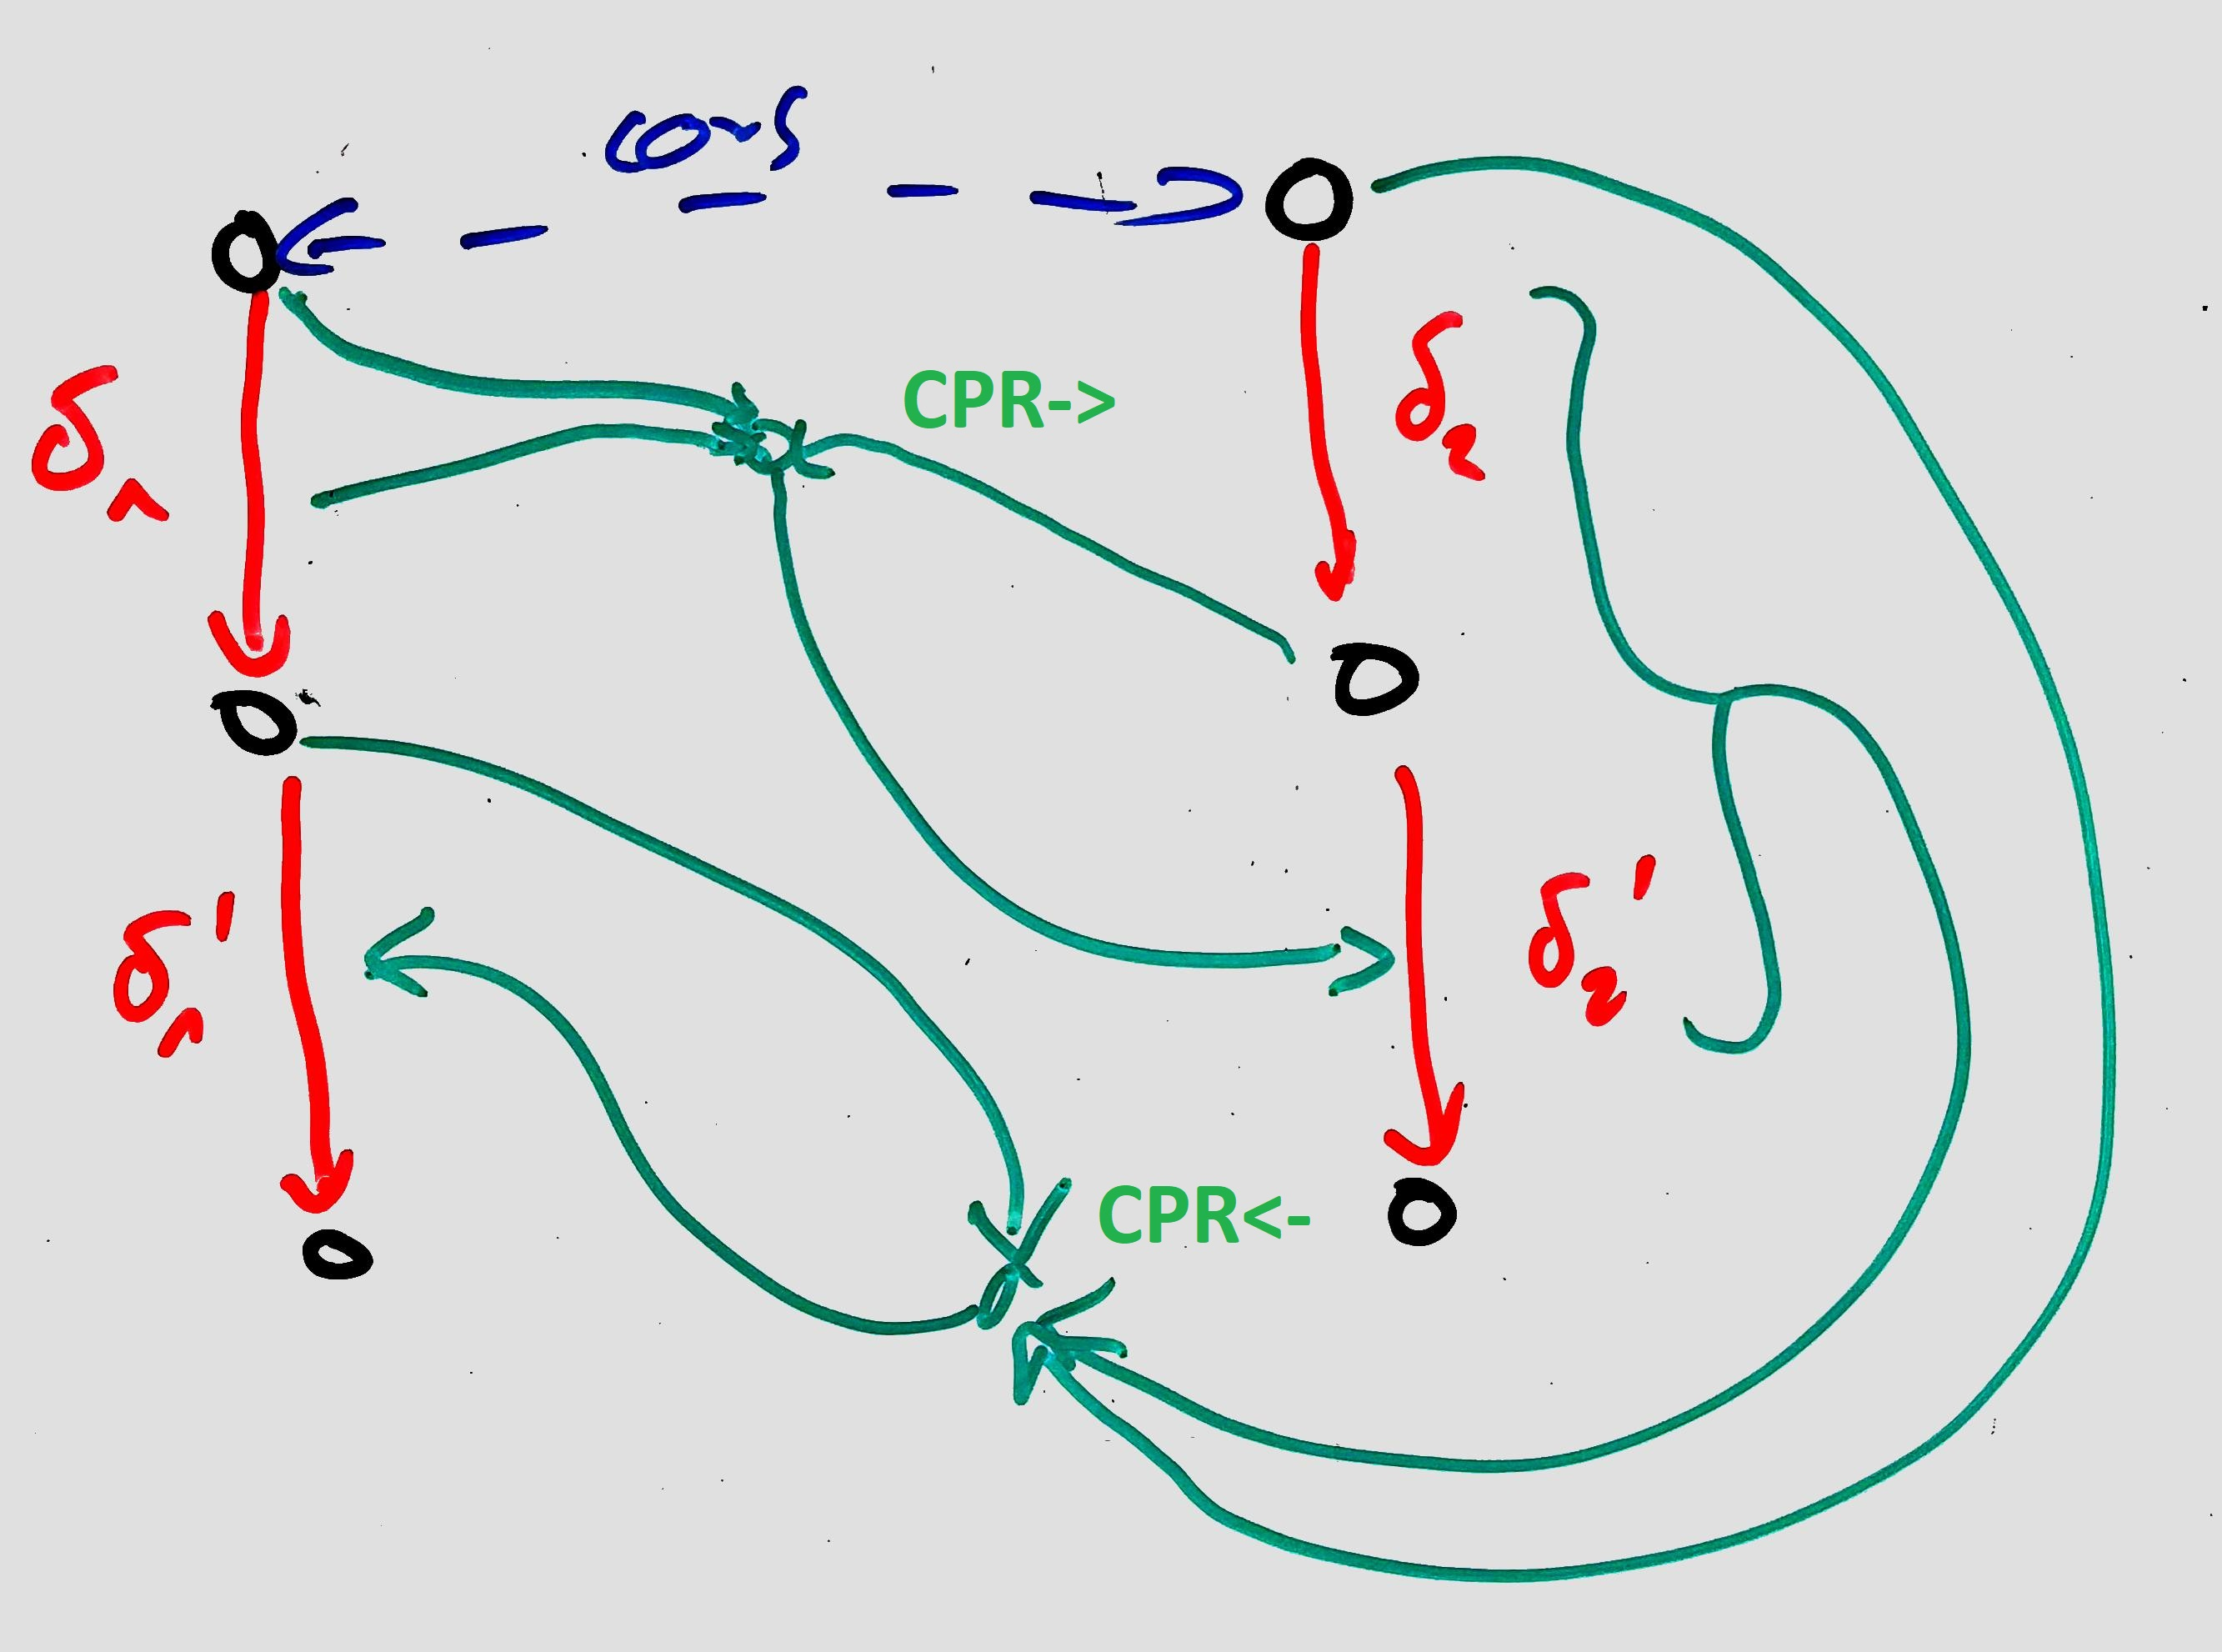
\includegraphics[width=0.7\textwidth]{figures/correctness/synchronization/synchronizing_execution_step.jpg}    
    \caption[Synchronizing bidirectional transformation execution step]{Operation of a synchronizing bidirectional transformation execution step}
    \label{fig:synchronization:synchronizing_execution_step}
\end{figure}

\mnote{Execute step of a transformation to integrate changes to both models}
Since we want consider the case that both of the models instead of only one of them have been modified, we extend the approach to process changes to both models.
More precisely, we introduce a modified notion of transformation execution steps, which is able to process changes to both models.
The operation of that execution step is depicted in \autoref{fig:synchronization:synchronizing_execution_step}.
To this end, the first executed consistency preservation rule is applied to the first model and the change to it, but receives the modified state of the second model.
We have motivated the necessity not to apply the first consistency preservation rule to the unmodified second model in \autoref{chap:synchronization:combination:sequencing}.
Afterwards, we apply the second consistency preservation rule to the unmodified first model and introduce the modifications to the second model as the concatenation of the original change and the one introduced by the first consistency preservation rule.
This way, we ensure that all inconsistencies are introduced by changes that are processed by the consistency preservation rules, which was our requirement for practical applicability due to the necessity only to react to changes instead of processing arbitrarily inconsistent models states.

\begin{definition}[Synchronizing Bidirectional Transformation Execution Step]
    \label{def:synchronizingtransformationexecutionstep}
    Let $\transformation{T} = \tupled{\consistencyrelationset{CR}, \consistencypreservationrule{\consistencyrelationset{CR}}^{\rightarrow}, \consistencypreservationrule{\consistencyrelationset{CR}}^{\leftarrow}}$ be a bidirectional transformation for metamodels $\metamodel{M}{1}$ and $\metamodel{M}{2}$.
    A \emph{synchronizing execution step} $\function{SyncEx}_{\transformation{T}}^1$ of $\transformation{T}$ is a function:
    \begin{align*}
        \function{SyncEx}_{\transformation{T}}^1 : \; & (\metamodelinstanceset{M}{1}, \metamodelinstanceset{M}{2}, \changeuniverse{\metamodel{M}{1}}, \changeuniverse{\metamodel{M}{2}}) \rightarrow (\metamodelinstanceset{M}{1}, \metamodelinstanceset{M}{2}, \changeuniverse{\metamodel{M}{1}}) \cup \setted{\bot} \\
        & (\model{m}{1}, \model{m}{2}, \change{\metamodel{M}{1}}, \change{\metamodel{M}{2}}) \mapsto 
        \begin{cases} 
            (\model{m}{1}', \model{m}{2}', \change{\metamodel{M}{1}}') \\
            \bot
        \end{cases}
    \end{align*}
    with:
    \begin{align*}
        & \change{\metamodel{M}{2}}' = \consistencypreservationrule{\consistencyrelationset{CR}}^{\rightarrow}(\model{m}{1}, \change{\metamodel{M}{2}}(\model{m}{2}), \change{\metamodel{M}{1}}) %\\
        & \model{m}{1}' = \change{\metamodel{M}{1}}(\model{m}{1}) \\
        & \change{\metamodel{M}{1}}' = \consistencypreservationrule{\consistencyrelationset{CR}}^{\leftarrow}(\model{m}{2}, \model{m}{1}', \change{\metamodel{M}{2}}' \concatfunction \change{\metamodel{M}{2}}) %\\
        & \model{m}{2}' = \change{\metamodel{M}{2}}'(\change{\metamodel{M}{2}}(\model{m}{2}))
    \end{align*}
    If either consistency preservation rule is undefined for the input, i.e., $\consistencypreservationrule{\consistencyrelationset{CR}}^{\rightarrow}(\model{m}{1}, \change{\metamodel{M}{2}}(\model{m}{2}), \change{\metamodel{M}{1}}) = \bot$ or $\consistencypreservationrule{\consistencyrelationset{CR}}^{\leftarrow}(\model{m}{2}, \model{m}{1}', \change{\metamodel{M}{2}}' \concatfunction \change{\metamodel{M}{2}}) \bot$, then the execution is undefined, i.e., $\function{SyncEx}_{\transformation{T}}^1(\model{m}{1}, \model{m}{2}, \change{\metamodel{M}{1}}) = \bot$.
    % for given models $\model{m}{1} \in \metamodelinstanceset{M}{1}$, $\model{m}{2} \in \metamodelinstanceset{M}{2}$ and a change $\change{\metamodel{M}{1}} \in \changeuniverse{\metamodel{M}{1}}$ to $\model{m}{1}$ is the consecutive execution of $\consistencypreservationrule{\consistencyrelationset{CR}}^{\rightarrow}$ and $\consistencypreservationrule{\consistencyrelationset{CR}}^{\leftarrow}}$, i.e.
    % \begin{align*}
    %     & \change{\metamodel{M}{2}}' = \consistencypreservationrule{\consistencyrelationset{CR}}^{\rightarrow}(\model{m}{1}, \model{m}{2}, \change{\metamodel{M}{1}}) \\
    %     & \change{\metamodel{M}{1}}' = \consistencypreservationrule{\consistencyrelationset{CR}}^{\leftarrow}(\model{m}{2}, \change{\metamodel{M}{1}}(\model{m}{1}), \change{\metamodel{M}{2}}')
    % \end{align*}
    % with the resulting changes $\change{\metamodel{M}{1}}'$ and $\change{\metamodel{M}{2}}'$.
\end{definition}

\mnote{Synchronization step needs to be executed only once}
The synchronizing bidirectional execution step is necessary to first integrate the changes made in both models.
It is defined such that it only produces a change in the first model, such that afterwards ordinary transformation execution steps that only need to deal with a change to one model have to be applied.
This leads the \autoref{algo:synchronization:executesynchronizingbidirectionaltransformation} for the execution of a synchronizing bidirectional transformation.
%Step integrates both changes, comparable to ordinary step, but first treats changes to m2 as already applied, i.e., given models are inconsistent, then processes the changes in the opposite direction to generate necessary changes to restore consistency from them.

\begin{algorithm}
    \input{algorithms/correctness/synchronization/execute_synchronizing_bidirectional_transformation.tex}
    \caption[Execution of a bidirectional transformation for synchronization]{Execution of a bidirectional transformation in the synchronization case.}
    \label{algo:synchronization:executesynchronizingbidirectionaltransformation}
\end{algorithm}

\mnote{Synchronizing transformation execution has same properties than non-synchronizing one}
This algorithm has the same properties as the one for the non-synchronization case given in \autoref{algo:synchronization:executebidirectionaltransformation}.
It does always terminate and either returns $\bot$ or a consistent pair of models.

\begin{theorem}[Consistent Termination of Partial-Consistency-Improving Synchronizing Bidirectional Transformation Execution]
    \label{theorem:synchronizingbidirectionaltransformationconsistencytermination}
    Let $\transformation{T} = \tupled{\consistencyrelationset{CR}, \consistencypreservationrule{\consistencyrelationset{CR}}^{\rightarrow}, \consistencypreservationrule{\consistencyrelationset{CR}}^{\leftarrow}}$ be a partial-consistency-improving bidirectional transformation.
    Then \autoref{algo:synchronization:executesynchronizingbidirectionaltransformation} does always terminate and either returns $\bot$ or a consistent model pair.
\end{theorem}
\begin{proof}
    The algorithm is identical to \autoref{algo:synchronization:executebidirectionaltransformation}, except for Lines~\ref{algo:synchronization:executesynchronizingbidirectionaltransformation:line:synchronizationstart}--\ref{algo:synchronization:executesynchronizingbidirectionaltransformation:line:synchronizationend}, which add the initial synchronization step.
    These lines add a single return statement that can return $\bot$.
    Since the return statement not returning $\bot$ is still preceded by the while loop having the loop condition that the model pair needs to be inconsistent, the argument of the proof for \autoref{lemma:bidirectionaltransformationconsistency} regarding non-synchronizing bidirectional transformations ensuring that only consistent models are returned still applies.
    Thus, we know the algorithm either returns $\bot$ or a consistent model pair.

    Termination of the algorithm is guaranteed for the same reasons as for non-synchronizing bidirectional transformations as proven in \autoref{lemma:bidirectionaltransformationtermination}.
    Although the additional execution of $\function{SyncEx}$ may introduce further inconsistencies, the proof already considered that the models given to the while loop may be arbitrarily inconsistent.
    Thus, the inductive improvement in partial consistency through the while loop is given in the same way and thus, finally, the model pair becomes consistent.
\end{proof}

\mnote{Transformation only need to deal with inconsistencies introduced by changes}
Thus, we have proven that we can execute a bidirectional transformation that is partial-consistency-improving for two given models and changes to both of the, such that consistent models are delivered, as long as the transformation is able to process the changes.
In fact, we have already restricted the algorithm such that it must not be able to deal with arbitrarily inconsistent models, but only with models that are initially given, such that only the given changes introduce inconsistencies.
This is supposed to make it easier to define transformation in practice that fulfill the property of being partial-consistency-improving, as they can rely on the assumption that inconsistency is only introduced by the given changes.

\mnote{Definition of synchronizing bidirectional transformations}
With the insight that partial-consistency-improving bidirectional transformations can be used to integrate changes to both of two models and deliver consistent models based on that changes, we can define \emph{synchronizing bidirectional transformations} as bidirectional transformations with the property of being partial-consistency-improving.

\begin{definition}[Synchronizing Bidirectional Transformation]
    Let $\transformation{T}$ be a partial-consistency-improving bidirectional transformation.
    Then we call $\transformation{T}$ a \emph{synchronizing bidirectional transformation}.
\end{definition}

\mnote{Order of consistency preservation rules provides no conceptual benefit but may improve usability}
As we have already discussed at the end of \autoref{chap:synchronization:bidirectional:transformations}, we defined bidirectional transformation execution steps starting with $\consistencypreservationrule{\consistencyrelationset{CR}}^{\rightarrow}$, although it may also be necessary to start with $\consistencypreservationrule{\consistencyrelationset{CR}}^{\leftarrow}$ if a change was performed in the second model.
We discussed that our definitions are without loss of generality and can be directly transferred by swapping the rules.
For the synchronization case, in which both models have been modified, it does, theoretically, not even make a difference which of the consistency preservation rules is executed first, because changes to both models are present anyway.
From a practical perspective, it can, however, make sense to define one the consistency preservation rules as the one to always be executed first.
For example, it might make sense to first execute the consistency preservation rule from the more abstract to the more detailed model, if such a relation exists between the models.
We leave such considerations up to the individual transformation developer or future research, as the selection of the order does not provide any conceptual benefits, but, in the best case, eases the definition of appropriate consistency preservation rules and improves usability.

\todo{Define synchronizing bidirectional transformation as a partial-consistency-improving bidirectional transformation}


\subsection{Equivalence to Synchronizing Transformations}

\mnote{Synchronizing and synchronizing bidirectional transformations have equal inputs and outputs}
For our definition of transformation networks, we used the notion of synchronizing transformations (cf.~\autoref{def:synchronizingtransformation}), whose single consistency preservation rule accept two consistent models and a change to each of them and return two changes that, if applied to the models, result in consistent models again.
Synchronizing bidirectional transformations, i.e., the yet defined transformations, which are composed of two unidirectional consistency preservation rules, also accept two consistent models and a change to each of them and return two consistent models.
We could also define those transformations to return changes rather than the consistent models by simply concatenating all changes calculated by the transformation execution steps.
For reasons of simplicity, we omitted that in the formal description.

\mnote{Synchronizing and synchronizing bidirectional transformations have equal expressiveness}
Although synchronizing transformations and synchronizing bidirectional transformations have the same requirements to their inputs and provide the same guarantees regarding consistency for their output, both may also return $\bot$ to indicate that they were not able to calculate changes that lead to consistent models.
While a synchronizing transformation can be defined such that it never return $\bot$ by defining a consistency preservation rule that is a total function, the possibility of a synchronizing bidirectional transformation to never return $\bot$ depends on the interplay of the two unidirectional consistency preservation rules.
Nevertheless, we can show that both have equal expressiveness, i.e., they can always return the same results for the same inputs.

\begin{theorem}[Synchronizing Bidirectional Transformation Expressiveness]
    Synchronizing bidirectional transformations have equal expressiveness than synchronizing transformations.
\end{theorem}
\begin{proof}
    Each synchronizing bidirectional transformation can be realized by a synchronizing transformation by simply defining the function of the consistency preservation rule such that it returns the result that is produced by the execution of the synchronizing bidirectional transformation.
    Let $\transformation{T}$ be a synchronizing bidirectional transformation with:
    \begin{align*}
        \function{ExecuteSync}(\transformation{T}, \model{m}{1}, \model{m}{2}, \change{\metamodel{M}{2}}) = (\model{m}{1}', \model{m}{2}')
    \end{align*}
    Then we define the consistency preservation rule $\consistencypreservationrule{}$ of a synchronizing transformation as:
    \begin{align*}
        &
        \consistencypreservationrule{}(\model{m}{1}, \model{m}{2}, \change{\metamodel{M}{1}}, \change{\metamodel{M}{2}}) = (\model{m}{1}, \model{m}{2}, \change{\metamodel{M}{1}}', \change{\metamodel{M}{2}}') \\
        & \formulaskip
        \mathtext{with} \change{\metamodel{M}{1}}'(\change{\metamodel{M}{1}}(\model{m}{1})) \equivalentperdefinition \model{m}{1}' 
        \land \change{\metamodel{M}{2}}'(\change{\metamodel{M}{2}}(\model{m}{2})) \equivalentperdefinition \model{m}{2}'
    \end{align*}
    Then, per definition, applying the resulting changes to the input models, the synchronizing transformation delivers for every possible input the same result by applying $\consistencypreservationrule{}$ as the synchronizing bidirectional transformation.

    Realizing a synchronizing transformation by a synchronizing bidirectional transformation requires the repeated execution of the two consistency preservation rules to emulate the behavior of the single 
    synchronizing consistency preservation rule.
    Let $\consistencypreservationrule{}$ be the consistency preservation rule of a synchronizing transformation with:
    \begin{align*}
        \consistencypreservationrule{}(\model{m}{1},\model{m}{2},\change{\metamodel{M}{1}},\change{\metamodel{M}{2}}) = (\model{m}{1},\model{m}{2},\change{\metamodel{M}{1}}',\change{\metamodel{M}{2}}')
    \end{align*}
    Then we can define the two unidirectional consistency preservation rules of the synchronizing transformation $\transformation{T}$ as follows.
    \begin{align*}
        & 
        \consistencypreservationrule{}^{\rightarrow}(\model{m}{1},\change{\metamodel{M}{2}}(\model{m}{2}),\change{\metamodel{M}{1}}) = \change{\metamodel{M}{2}}'' \mathtext{with} \change{\metamodel{M}{2}}''(\change{\metamodel{M}{2}}(\model{m}{2})) \equivalentperdefinition \change{\metamodel{M}{2}}'(\model{m}{2}) \\
        &
        \consistencypreservationrule{}^{\leftarrow}(\model{m}{2},\change{\metamodel{M}{1}}(\model{m}{1}),\change{\metamodel{M}{2}}'' \concatfunction \change{\metamodel{M}{2}}) = \change{\metamodel{M}{1}}'' \mathtext{with} \change{\metamodel{M}{1}}''(\change{\metamodel{M}{1}}(\model{m}{1})) \equivalentperdefinition \change{\metamodel{M}{1}}'(\model{m}{1})
    \end{align*}
    So we simply define the two consistency preservation rules in a way such that each of them delivers for the inputs in the synchronizing execution step $\function{SyncEx}_{\transformation{T}}^1$ according to \autoref{def:synchronizingtransformationexecutionstep} those changes that are necessary to produce exactly the results of the consistency preservation rule $\consistencypreservationrule{}$ of the synchronizing transformation.
    Then according to the behavior of $\function{SyncEx}_{\transformation{T}}^1$, we have:
    \todo{Vielleicht besser Striche über Buchstaben statt noch mehr Apostrophe}
    \begin{align*}
        &
        \function{SyncEx}_{\transformation{T}}^1(\model{m}{1},\model{m}{2},\change{\metamodel{M}{1}},\change{\metamodel{M}{2}}) = (\model{m}{1}'', \model{m}{2}'', \change{\metamodel{M}{1}}''') \mathtext{with} \\
        & \formulaskip
        \change{\metamodel{M}{1}}'''(\model{m}{1}'') = % per def SyncEx
        \change{\metamodel{M}{1}}'''(\change{\metamodel{M}{1}}(\model{m}{1})) = % per def SyncEx and per def above
        %\consistencypreservationrule{}^{\leftarrow}(\model{m}{2},\change{\metamodel{M}{1}}(\model{m}{1}),\change{\metamodel{M}{2}}'' \concatfunction \change{\metamodel{M}{2}})(\change{\metamodel{M}{1}}(\model{m}{1})) % per def above
        \change{\metamodel{M}{1}}'(\model{m}{1}) \\
        & \formulaskip
        \land
        \model{m}{2}'' = \change{\metamodel{M}{2}}'(\model{m}{2})
    \end{align*}
    So $\function{SyncEx}_{\transformation{T}}^1$ produces $\model{m}{1}''$, $\model{m}{2}''$ and $\change{\metamodel{M}{1}}'''$ for which we know that $\change{\metamodel{M}{1}}'''(\model{m}{1}'')$ and $\model{m}{2}''$ are consistent, because their equivalents $\change{\metamodel{M}{1}}'(\model{m}{1})$ and $\change{\metamodel{M}{2}}'(\model{m}{2})$ are consistent by assumption.
    Thus, the execution of the synchronizing bidirectional transformation $\transformation{T}$ according to \autoref{algo:synchronization:executesynchronizingbidirectionaltransformation} terminates after the conditional statement in \autoref{algo:synchronization:executesynchronizingbidirectionaltransformation:line:synchronizationstart} with the same consistent models that are delivered by the applying the changes calculated by the consistency preservation rule $\consistencypreservationrule{}$ of the assumed synchronizing transformation.

    With these construction approaches in both directions, we have shown that each synchronizing transformation can be expressed by a synchronizing bidirectional transformation and vice versa.
\end{proof}

\mnote{Executing only one synchronizing execution step will not lead to consistency in pratice}
Although we have proven that each synchronizing transformation can be expressed by a synchronizing bidirectional transformations and thus the latter ones can be used to express any desired consistency preservation in a transformation network, the constructive approach in the proof does not reflect a practical construction approach for the unidirectional consistency preservation rules of a synchronizing bidirectional transformation.
In practice, it will usually not be possible to define the rules in a way that they deliver consistent models after executing each ones, as we already discussed in \autoref{chap:synchronization:combination:bounds}.
It shows, however, that it would possible in theory.

\mnote{Synchronizing bidirectional transformations can be used in transformation networks}
Based on the knowledge that we can use synchronizing bidirectional transformations in transformation networks, we discuss in the following how a transformation developer can actually achieve that the specification of a bidirectional transformation in terms of two unidirectional consistency preservation rules does actually fulfill the requirements of being partial-consistency-improving and thus synchronizing.


% We yet discussed how to integrate one change on partially consistent models.
% Now we apply to this be able to integrate changes to both models.
% Describe the process here:

% Two step process.
% 1 Integrate changes to both models.
% d2' = CPRr(m1, d2(m2), d1) und d1' = CPRl(m2, d1(m1), d2' o d2)
% 2. Iteratively propagate changes.
% d2'' = CPRr(d1(m1), d2' o d2(m2), d1')
% d1'' = CPRl(d2' o d2(m2), d1(m1), d2'')
% etc. 

% The first step is special, because CPRl needs to process both the original changes as well as the ones generated by CPRr in the first step.
% In all further steps it is only necessary to process the changes just generated by the other CPR.

% DISCUSS: Which CPR to execute first? One is the "leading" one. Integrate its changes first. Can be determined by abstraction, or, theoretically, it completely irrelevant. Only a practical consideration.



% \section{Old contents to integrate}

%%
%% THE DIRECTIONALITY GAP: Formal framework considers bidirectional transformations, practically we have unidirectional ones
%%
% \subsection{The Directionality Gap}

% \mnote{Unidirectional synchronizing preservation rules to close the gap}
% To come up with an approach to combine unidirectional consistency preservation rules to behave as a single synchronizing one, we first identify how we can decompose synchronizing consistency preservation rules into unidirectional ones.
% We then relate these unidirectional synchronizing rules to the non-synchronizing ones defined in transformation languages.

% \mnote{Fine-grained consistency relations allow to define relation between unidirectional preservation rules}
% In \autoref{chap:compatibility:formal_notion}, we also discussed that consistency relation can be considered in a fine-grained way that is able to reflect different notion of consistency in both directions of a relation.
% We will base our notion of unidirectional synchronizing rules on those fine-grained relations to be able to find a proper notion of how the rules in both directions are supposed to work together.
% We did, however, also discuss in that chapter that all fine-grained relations can also be translated into \modellevelconsistencyrelations, thus the insights we already had for those model-level relations still apply to the considerations regarding fine-grained ones.

% \mnote{Stick to coarse-grained notion of preservation rules}
% According to the consideration of fine-grained consistency relations, transformation languages also allow the specification of or derive fine-grained consistency preservation rules from a declarative specification.
% They are often called \emph{transformation rules} and composed to a transformation that consists of multiple such rules, each encoding a consistency relations and a preservation rule for it.
% We will, however, stick to the coarse-grained notion of consistency preservation rules, as they are sufficient for our considerations.

% \mnote{New transformation notion based on fine-grained consistency relations}
% In consequence, from now we will consider a synchronizing transformation as a set of fine-grained consistency relations according to \autoref{def:consistencyrelation} and a consistency preservation rule that preserves consistency according to the set of relations.
% The consistency preservation rule and also the complete transformation are thus still considered correct if applying it to a consistent pair of models and changes to them, applying the resulting changes to the models again delivers a pair of models that is consistent to all consistency relations.
% Note that being consistent to all fine-grained consistency relations is equivalent to being consistent to the single \modellevelconsistencyrelation induced by the fine-grained relations.


% \subsubsection{Unidirectional Synchronizing Transformations}

% \mnote{Decomposition of consistency preservation rules into two unidirectional ones}
% To reflect the unidirectional notion of consistency preservation provided by transformation languages in our formalism, we propose a decomposition of consistency preservation rules according to \autoref{def:consistencypreservationrule} into two unidirectional ones.

% \begin{definition}[Unidirectional Consistency Preservation Rule]
%     \label{def:unidirectionalconsistencypreservationrule}
%     Let $\metamodel{M}{1}, \metamodel{M}{2}$ be two metamodels and $\consistencyrelationset{CR}$ a set of consistency relations between elements of those metamodels.
%     A \emph{unidirectional consistency preservation rule} $\consistencypreservationrule{\consistencyrelationset{CR}}$ for the relation set $\consistencyrelationset{CR}$ is a function:
%     \begin{align*}
%         \consistencypreservationrule{\consistencyrelationset{CR}} : (\metamodelinstanceset{M}{1}, \metamodelinstanceset{M}{2}, \changeuniverse{\metamodel{M}{1}}, \changeuniverse{\metamodel{M}{2}}) \rightarrow \changeuniverse{\metamodel{M}{2}}
%     \end{align*}
% \end{definition}

% \mnote{Notation for two related unidirectional rules}
% To be able to explicitly reference the consistency preservation rules for both directions between two metamodels $\metamodel{M}{1}$ and $\metamodel{M}{2}$, we denote the set of consistency relations between $\metamodel{M}{1}$ and $\metamodel{M}{2}$ as $\consistencyrelationset{CR}_{\rightarrow}$ and the one in the opposite direction between $\metamodel{M}{2}$ and $\metamodel{M}{1}$ as $\consistencyrelationset{CR}_{\leftarrow}$.
% We then refer to the two unidirectional consistency preservation rules as:
% \begin{align*}
%     \consistencypreservationrule{\consistencyrelationset{CR}_{\rightarrow}} : (\metamodelinstanceset{M}{1}, \metamodelinstanceset{M}{2}, \changeuniverse{\metamodel{M}{1}}) \rightarrow \changeuniverse{\metamodel{M}{2}}\\
%     \consistencypreservationrule{\consistencyrelationset{CR}_{\leftarrow}} : (\metamodelinstanceset{M}{2}, \metamodelinstanceset{M}{1}, \changeuniverse{\metamodel{M}{2}}) \rightarrow \changeuniverse{\metamodel{M}{1}}
% \end{align*}

% \mnote{Correctness of unidirectional rules analogous to original rules}
% We define correctness of such a unidirectional consistency preservation rule in the same way it was defined for synchronizing consistency preservation rules according to \autoref{def:consistencypreservationrule} and compliant to existing correctness notions for non-synchronizing consistency preservation rules, such as~\cite{stevens2010sosym}.

% \begin{definition}[Unidirectional Consistency Preservation Rule Correctness]
%     \label{def:unidirectionalconsistencypreservationrulecorrectness}
%     Let $\consistencypreservationrule{\consistencyrelationset{CR}}$ be a \emph{unidirectional consistency preservation rule}.
%     We call $\consistencypreservationrule{\consistencyrelationset{CR}}$ \emph{correct} if the resulting models when applying the generated changes are consistent to $\consistencyrelationset{CR}$ again:
%     \begin{align*}
%         &
%         \forall 
%         \model{m}{1} \in \metamodelinstanceset{M}{1}, 
%         \model{m}{2} \in \metamodelinstanceset{M}{2},
%         \change{\metamodel{M}{1}} \in \changeuniverse{\metamodel{M}{1}},
%         \change{\metamodel{M}{2}} \in \changeuniverse{\metamodel{M}{2}} : \\
%         & \formulaskip
%         \tupled{\model{m}{1}, \model{m}{2}} \consistenttomath \consistencyrelationset{CR} \\
%         & \formulaskip
%         \land \exists 
%         \change{\metamodel{M}{2}}' \in \changeuniverse{\metamodel{M}{2}} :
%         \change{\metamodel{M}{2}}' = \consistencypreservationrule{\consistencyrelation{CR}{}}(\model{m}{1}, \model{m}{2}, \change{\metamodel{M}{1}}, \change{\metamodel{M}{2}}) \\
%         & \formulaskip\formulaskip
%         \Rightarrow
%         \tupled{\change{\metamodel{M}{1}}(\model{m}{1}), \change{\metamodel{M}{2}}'(\model{m}{2})} \consistenttomath \consistencyrelationset{CR}
%     \end{align*}
% \end{definition}

% \mnote{Unidirectional synchronizing transformation encapsule a preservation rule for each direction}
% Based on such a unidirectional notion of consistency preservation rule, we can also define a unidirectional notion of transformations, which then consists of two sets of unidirectional consistency relations and two unidirectional consistency preservation rules.

% \begin{definition}[Unidirectional Synchronizing Transformation]
%     \label{def:unidirectionalsynchronizingtransformation}
%     Let $\metamodel{M}{1}$ and $\metamodel{M}{2}$ be two metamodels and $\consistencyrelationset{CR}_{\rightarrow}$ a set of consistency relations between $\metamodel{M}{1}$ and $\metamodel{M}{2}$, as well as $\consistencyrelationset{CR}_{\leftarrow}$ a set of consistency relations between $\metamodel{M}{2}$ and $\metamodel{M}{1}$.
%     Additionally, let $\consistencypreservationrule{\consistencyrelationset{CR}_{\rightarrow}}$ and $\consistencypreservationrule{\consistencyrelationset{CR}_{\leftarrow}}$ be unidirectional consistency preservation rules for both consistency relation sets.
%     A \emph{unidirectional synchronizing transformation} is a quadruple $\transformation{T} = \tupled{\consistencyrelationset{CR}_{\rightarrow}, \consistencyrelationset{CR}_{\leftarrow},\consistencypreservationrule{\consistencyrelationset{CR}_{\rightarrow}}, \consistencypreservationrule{\consistencyrelationset{CR}_{\leftarrow}}}$.
% \end{definition}

% \mnote{Correctness of unidirectional synchronizing transformations}
% We call such a unidirectional synchronizing transformation correct if both consistency preservation rules are correct, i.e., they both preserve consistency according to the underlying consistency relation set.

% \begin{definition}[Unidirectional Synchronizing Transformation Correctness]
%     \label{def:unidirectionalsynchronizingtransformationcorrectness}
%     Let $\transformation{T} = \tupled{\consistencyrelationset{CR}_{\rightarrow}, \consistencyrelationset{CR}_{\leftarrow},\consistencypreservationrule{\consistencyrelationset{CR}_{\rightarrow}}, \consistencypreservationrule{\consistencyrelationset{CR}_{\leftarrow}}}$ be a unidirectional synchronizing transformation.
%     We call $\transformation{T}$ correct if, and only if, $\consistencypreservationrule{\consistencyrelationset{CR}_{\rightarrow}}$ and $\consistencypreservationrule{\consistencyrelationset{CR}_{\leftarrow}}$ are both correct according to \autoref{def:unidirectionalconsistencypreservationrulecorrectness}.
% \end{definition}

% \mnote{Each unidirectional rule only preserves consistency in one direction}
% With a unidirectional synchronizing transformation that adheres to the given correctness definition, we are able to preserve consistency for the consistency relations in each direction between two models.
% Executing either of the unidirectional consistency preservation rules of the transformation does, however, not ensure that the consistency relations for the other direction are fulfilled as well.
% That is the purpose of the other unidirectional consistency preservation rule.

% % \begin{itemize}
%     % \item We assume consistency preservation rules according to fine-grained consistency relations introduced for compatibility
%     % \item So a synchronizing transformation considers fine-grained relations, in fact a transformation then consists of multiple relations, two for each fine-grained relation (each direction). Their combination induces the \modellevelconsistencyrelation for the two metamodels.
%     % \item Although the consistency preservation rule may in practice also be defined in terms fine-grained rules, which together with the fine-grained consistency rules then forms what is often called \emph{transformation rules}, we do not need to have a more fine-grained notion here.
%     % \item The transformation then is still correct as defined before, when the preservation rule preserves consistency to the relation, but now according to all fine-grained relations (and thus also the induced monolithic one) instead to the single model-level one.
%     % \item To reflect the notion of unidirectional consistency preservation rules, as often defined in transformation languages, which are still synchronizing, i.e., are able to react to changes made to both models, we may define:
% % \end{itemize}
% % \begin{align*}
% %     \consistencypreservationrule{\consistencyrelationset{CR}_{\rightarrow},\rightarrow} : (\metamodelinstanceset{M}{1}, \metamodelinstanceset{M}{2}, \changeuniverse{\metamodel{M}{1}}, \changeuniverse{\metamodel{M}{2}}) \rightarrow \changeuniverse{\metamodel{M}{2}})\\
% %     \consistencypreservationrule{\consistencyrelationset{CR}_{\leftarrow},\leftarrow} : (\metamodelinstanceset{M}{1}, \metamodelinstanceset{M}{2}, \changeuniverse{\metamodel{M}{1}}, \changeuniverse{\metamodel{M}{2}}) \rightarrow \changeuniverse{\metamodel{M}{1}})
% % \end{align*}

% \subsubsection{Alignment of Unidirectional Synchronizing Transformations}

% \mnote{Sequential execution of unidirectional rules does not guarantee consistency to relations in both directions}
% It is now possible to execute both consistency preservation rules of a unidirectional synchronizing transformation one after another, as each is able to reflect the changes produced by the other due to the ability to process changes made to both models.
% Thus, we could sequentially calculate:
% \begin{align*}
%     &
%     \change{\metamodel{M}{2}}' = \consistencypreservationrule{\consistencyrelationset{CR}_{\rightarrow}}(\model{m}{1},\model{m}{2},\change{\metamodel{M}{1}},\change{\metamodel{M}{2}})\\
%     &
%     \change{\metamodel{M}{1}}' = \consistencypreservationrule{\consistencyrelationset{CR}_{\leftarrow}}(\model{m}{2},\model{m}{1},\change{\metamodel{M}{2}}',\change{\metamodel{M}{1}})
% \end{align*}
% We then receive the resulting model pair as $\tupled{\change{\metamodel{M}{1}}'(\model{m}{1}), \change{\metamodel{M}{2}}'(\model{m}{2})}$.
% This gives us the guarantee that the resulting model pair is consistent to $\consistencyrelationset{CR}_{\leftarrow}$, as its consistency preservation rule was executed last.
% However, the definitions do not give any guarantee that the model pair is consistent to $\consistencyrelationset{CR}_{\rightarrow}$, as the execution of $\consistencypreservationrule{\consistencyrelationset{CR}_{\leftarrow}}$ may violate some of those relations.

% \mnote{Not violating relations of the other direction is desirable for unidirectional rules}
% It is, however, a desirable property of a unidirectional synchronizing transformation that the consistency preservation rules for the two directions between the same metamodels are aligned with each other in a way that executing the rule in one direction does not lead to further violations of the consistency relations in the other direction.
% This is especially necessary to produce the same behavior as a synchronizing transformation.
% We call such a property \emph{inverse-preserving}, as it ensures that fulfillment of consistency relations of the inverse direction are preserved.

% \begin{definition}[Inverse-Preserving Unidirectional Synchronizing Transformation]%Unidirectional Consistency Preservation Rule}
%     \label{def:inversepreservingunidirectionalsynchronizingtransformation}
%     Let $\transformation{T} = \tupled{\consistencyrelationset{CR}_{\rightarrow}, \consistencyrelationset{CR}_{\leftarrow},\consistencypreservationrule{\consistencyrelationset{CR}_{\rightarrow}}, \consistencypreservationrule{\consistencyrelationset{CR}_{\leftarrow}}}$ be a correct unidirectional synchronizing transformation for two metamodels $\metamodel{M}{1}$ and $\metamodel{M}{2}$.
%     We say that $\transformation{T}$ is \emph{inverse-preserving} if, and only if, executing one of the consistency preservation rules ensures that the resulting models are still consistent to all consistency relations of the opposite direction to which the models were consistent before.
%     For $\consistencypreservationrule{\consistencyrelationset{CR}_{\rightarrow}}$ this is given by the following (for $\consistencypreservationrule{\consistencyrelationset{CR}_{\leftarrow}}$ analogously):
%     \begin{align*}
%         & \forall \model{m}{1} \in \metamodelinstanceset{M}{1}, \model{m}{2} \in \metamodelinstanceset{M}{2}, \change{\metamodel{M}{1}} \in \changeuniverse{\metamodel{M}{1}}, \change{\metamodel{M}{2}} \in \changeuniverse{\metamodel{M}{2}} : \\
%         & 
%         \exists \change{\metamodel{M}{2}}' \in \changeuniverse{\metamodel{M}{2}} : \change{\metamodel{M}{2}}' = \consistencypreservationrule{\consistencyrelationset{CR}_{\rightarrow}}(\model{m}{1},\model{m}{2},\change{\metamodel{M}{1}},\change{\metamodel{M}{2}}) \\
%         & \formulaskip
%         \Rightarrow
%         \forall \consistencyrelation{CR}{} \in \consistencyrelationset{CR}_{\leftarrow}: 
%         \bigl(
%         \tupled{\change{\metamodel{M}{2}}(\model{m}{2}),\change{\metamodel{M}{1}}(\model{m}{1})} \consistenttomath \consistencyrelation{CR}{} \\
%         & \formulaskip\formulaskip
%         \Rightarrow
%         \tupled{\change{\metamodel{M}{2}}'(\model{m}{2}), \change{\metamodel{M}{1}}(\model{m}{1})} \consistenttomath \consistencyrelation{CR}{}
%         \bigr)
%     \end{align*}
% \end{definition}

% \mnote{Inverse-preserving transformations define reasonable alignment}
% This is a reasonable property, because the consistency relations in both directions are usually not disaligned, but only give the freedom to define different consistency notions in both directions, such as more options for consistent elements in one direction than in the other to support different kinds of abstraction.
% It should, however, never be the case that preserving consistency in one direction violates consistency relations in the other direction if transformations are defined properly.

% \mnote{Inverse-preserving transformations can be sequences}
% Given an inverse-preserving unidirectional synchronizing transformation, executing the two unidirectional consistency preservation rules one after another to given consistent models and changes to them preserves consistency to all consistency relations.
% This is a direct consequence of the inverse-preserving property, because no directional rule is allowed to violate consistency that was already ensured in the other direction.

% \begin{theorem}[Inverse-Preserving Unidirectional Synchronizing Transformation Sequencing Correctness]
%     \label{theorem:sequencinginversepreservingtransformations}
%     Let $\transformation{T} = \tupled{\consistencyrelationset{CR}_{\rightarrow}, \consistencyrelationset{CR}_{\leftarrow}, \consistencypreservationrule{\consistencyrelationset{CR}_{\rightarrow}}, \consistencypreservationrule{\consistencyrelationset{CR}_{\leftarrow}}}$ be a correct, inverse-preserving unidirectional synchronizing transformation.
%     Then sequentially executing both consistency preservation rules to given models and changes restores consistency to both consistency relation sets, i.e., given models $\model{m}{1}, \model{m}{2}$ and changes to them $\change{\metamodel{M}{1}}, \change{\metamodel{M}{2}}$, it holds hat:
%     \begin{align*}
%         &
%         \tupled{\model{m}{1}, \model{m}{2}} \consistenttomath \consistencyrelationset{CR}_{\rightarrow}
%         \land \tupled{\model{m}{2}, \model{m}{1}} \consistenttomath \consistencyrelationset{CR}_{\leftarrow}\\
%         &
%         \land \exists \change{\metamodel{M}{2}}' \in \changeuniverse{\metamodel{M}{2}}' : 
%         \change{\metamodel{M}{2}}' = \consistencypreservationrule{\consistencyrelationset{CR}_{\rightarrow}}(\model{m}{1}, \model{m}{2}, \change{\metamodel{M}{1}}, \change{\metamodel{M}{2}}) \\
%         &
%         \land \exists \change{\metamodel{M}{1}}' \in \changeuniverse{\metamodel{M}{1}}' :
%         \change{\metamodel{M}{1}}' = \consistencypreservationrule{\consistencyrelationset{CR}_{\leftarrow}}(\model{m}{2}, \model{m}{1}, \change{\metamodel{M}{2}}', \change{\metamodel{M}{1}}) \\
%         &
%         \Rightarrow \tupled{\change{\metamodel{M}{1}}'(\model{m}{1}), \change{\metamodel{M}{2}}'(\model{m}{2})}\consistenttomath \consistencyrelationset{CR}_{\rightarrow}  \\
%         & \formulaskip
%         \land \tupled{\change{\metamodel{M}{2}}'(\model{m}{2}), \change{\metamodel{M}{1}}'(\model{m}{1})} \consistenttomath \consistencyrelationset{CR}_{\leftarrow}
%     \end{align*}
% \end{theorem}
% \begin{proof}
%     Given models $\model{m}{1}, \model{m}{2}$ that are consistent to $\consistencyrelationset{CR}_{\rightarrow}$ and $\consistencyrelationset{CR}_{\leftarrow}$ and changes $\change{\metamodel{M}{1}}, \change{\metamodel{M}{2}}$, we assume that $\change{\metamodel{M}{1}}'$ and $\change{\metamodel{M}{2}}'$ exist as the results of the consistency preservation rules according to the theorem.
%     If this was not the case, the consistency preservation rules are not defined for the given inputs and thus are not able to produce consistent results, which evaluates the left side of the implication to false, making the whole statement of the theorem true.
%     Now we show correctness of both implied statements:
%     \begin{properenumerate}
%         \item $\tupled{\change{\metamodel{M}{1}}'(\model{m}{1}), \change{\metamodel{M}{2}}'(\model{m}{2})}\consistenttomath \consistencyrelationset{CR}_{\rightarrow}$:
%         As a direction implication of correctness of $\consistencypreservationrule{\consistencyrelationset{CR}_{\rightarrow}}$, we know that $\tupled{\change{\metamodel{M}{1}}(\model{m}{1}), \change{\metamodel{M}{2}}'(\model{m}{2})} \consistenttomath \consistencyrelationset{CR}_{\rightarrow}$.
%         Now the inverse-preserving property of $\transformation{T}$ ensures for the given input of $\consistencypreservationrule{\consistencyrelationset{CR}_{\leftarrow}}$ according to \autoref{def:inversepreservingunidirectionalsynchronizingtransformation} that 
%         \begin{align*}
%         & \forall \consistencyrelation{CR}{} \in \consistencyrelationset{CR}_{\rightarrow}: 
%         \bigl(
%         \tupled{\change{\metamodel{M}{1}}(\model{m}{1}),\change{\metamodel{M}{2}}'(\model{m}{2})} \consistenttomath \consistencyrelation{CR}{} \\
%         & \formulaskip\formulaskip
%         \Rightarrow
%         \tupled{\change{\metamodel{M}{1}}'(\model{m}{2}), \change{\metamodel{M}{2}}'(\model{m}{1})} \consistenttomath \consistencyrelation{CR}{}
%         \bigr)
%         \end{align*}
%         Since the left side of the implication is true for all consistency relations in $\consistencyrelationset{CR}_{\rightarrow}$ due to correctness of $\consistencypreservationrule{\consistencyrelationset{CR}_{\rightarrow}}$, the right side is also true for all consistency relations in $\consistencyrelationset{CR}_{\rightarrow}$.
%         In consequence, we know that $\tupled{\change{\metamodel{M}{1}}'(\model{m}{1}), \change{\metamodel{M}{2}}'(\model{m}{2})} \consistenttomath \consistencyrelationset{CR}_{\rightarrow}$
%         \item $\tupled{\change{\metamodel{M}{2}}'(\model{m}{2}), \change{\metamodel{M}{1}}'(\model{m}{1})} \consistenttomath \consistencyrelationset{CR}_{\leftarrow}$:
%         This directly follows from correctness of $\consistencypreservationrule{\consistencyrelationset{CR}_{\leftarrow}}$.
%     \end{properenumerate}
%     In consequence, sequentially applying both consistency preservation rules of an inverse-preserving unidirectional synchronizing transformation ensures consistency to the consistency relations in both directions.
% \end{proof}

% \mnote{Inverse-preserving unidirectional transformation can emulate synchronizing ones}
% As a consequence of the theorem, we know that we can emulate a synchronizing transformation according to \autoref{def:synchronizingtransformation} with an inverse-preserving unidirectional synchronizing transformation according to \autoref{def:inversepreservingunidirectionalsynchronizingtransformation}.
% We can execute the unidirectional consistency preservation rules one after another to achieve that the resulting models are consistent to all consistency relations in both direction.

% \mnote{Ensuring inverse-preserving property is already a problem of bidirectional transformations}
% In fact, it is not trivial to ensure that two unidirectional transformations are inverse-preserving, even if the consistency relations in both directions are the same, which we will also see in our evaluation of errors in \autoref{chap:errors}.
% This problem, however, already arises when defining bidirectional transformations.
% Transformation languages may derive two unidirectional preservation rules from one specification, so that they are inherently inverse-preserving, or they may allow individual specification of the directions and provide some support for checking that they are aligned with each other, e.g., in the sense that they are inverse-preserving.
% This is, however, an isolated and existing topic of research \todo{Add references for that} and a challenge that already has to be solved for a single bidirectional transformation rather than a network, which is why we do not discuss this problem in more detail here and therefore assume given transformations to be inverse-preserving.

% \mnote{Directionality gap was discussed, synchronization gap remains}
% We have discussed the gap between synchronizing transformations and ordinary transformations defined in transformation languages regarding directionality by decomposing synchronizing transformations into unidirectional ones.
% In the following, we discuss the remaining gap of the formalized transformations being synchronizing, whereas practically defined transformations do not have that property.


%%
%% THE SYNCHRONIZATION GAP: After the directionality gap, we need to discuss how to come from synchronizing to non-synchronizing transformations
%%
% \subsection{The Synchronization Gap}

% \mnote{Practical transformations are not synchronizing}
% Still, there is a gap to practical approaches for defining transformations, as existing approaches do usually not support synchronization, i.e., they are not able to process changes in both models, but only in one of them.
% Transformation languages usually assume that changes are either made by the developer and are then to be propagated to the other model by the transformation, or they are made by the transformation in reaction to changes to the other model.
% The case that developers modify multiple models is sometimes also referred to as a synchronization scenario (although the term is sometimes even used for the simple case of incremental update).
% If we consider that scenario, we will refer to it as \emph{concurrent editing} to avoid confusion.

% \mnote{In contrast to arbitrary concurrent changes, transformation networks produce less conflicts}
% Although the two cases have in common that both instead of only one model involved in a transformation may have been modified, they have a specific difference.
% While user changes to both models can be arbitrarily conflicting, changes performed by other transformations in a network should, in general, not be conflicting, especially if the underlying relations are compatible, as discussed in \autoref{chap:compatibility}.
% For example, if a user changes an element $A$, whose information needs to be propagated to element $B$, but removes element $B$ as well, this cannot be resolved easily, apart from potentially removing element $A$ as well.
% However, as we know from existing approaches for concurrent editing with tools like Git, conflict resolution is not a trivial task~\todo{add cite for difficulty of conflict resolution}.
% Such a scenario may, however, not occur in a transformation network, because if transformations remove elements that are to be updated by others, there will obviously be some conflicts in the transformations manifested in an incompatibility of their consistency relations.

% \mnote{Definition of ordinary transformations}
% An ordinary unidirectional consistency preservation rule as defined in or produced by a transformation language looks as follows:
% \begin{align*}
%     \consistencypreservationrule{\consistencyrelationset{CR}_{\rightarrow}} : (\metamodelinstanceset{M}{1}, \metamodelinstanceset{M}{2}, \changeuniverse{\metamodel{M}{1}}) \rightarrow \changeuniverse{\metamodel{M}{2}}
% \end{align*}
% Such a rule is not synchronizing, i.e., it does not consider that the second model was modified as well, like we defined for unidirectional consistency preservation rules in \autoref{def:unidirectionalconsistencypreservationrule}.

% \mnote{Passing changed models to consistency preservation rule is not possible}
% Given models $\model{m}{1},\model{m}{2}$ and changes $\change{\metamodel{M}{1}},\change{\metamodel{M}{2}}$, if we simply pass the changed model $\model{m}{2}$ to the preservation rule, we call $\consistencypreservationrule{\consistencyrelationset{CR}_{\rightarrow}}(\model{m}{1},\change{\metamodel{M}{2}}(\model{m}{2}),\change{\metamodel{M}{1}})$.
% Then, in general, the behavior of the function is undefined.
% As defined in \autoref{def:consistencypreservationrulecorrectness}, we only required the function to return a change such that applying all changes produces consistent models if the original models were consistent.
% In this case, however, the given models are not necessarily consistent to each other.

% %\subsection{Closing the Gap}
% \mnote{Emulate synchronizing transformations with non-synchronizing ones}
% We thus want to achieve a slight adaptation of those non-synchronizing unidirectional consistency preservation rules, such that they support the case that they support the synchronization case, i.e., that the second model has already been modified.
% Informally speaking, we want to emulate unidirectional synchronizing consistency preservation rules with non-synchronizing ones.
% Additionally, we want to ensure that if such a rule is inverse-preserving for consistent inputs, it is also inverse-preserving for the case that the second model was already modified, such that executing both rules consecutively ensures consistency to the relations in both directions, as we have already proven for inverse-preserving synchronizing transformations in \autoref{theorem:sequencinginversepreservingtransformations}.

% \mnote{Find requirements for non-synchronizing transformations to impose same behavior as synchronizing ones}
% We thus want to find out what has to be considered to define a pair of ordinary, non-synchronizing consistency preservation rules $\consistencypreservationrule{\consistencyrelationset{CR}_{\rightarrow}}$ $\consistencypreservationrule{\consistencyrelationset{CR}_{\leftarrow}}$ to emulate a unidirectional synchronizing transformation.
% This means that $\consistencypreservationrule{\consistencyrelationset{CR}_{\rightarrow}}$ is able to process an input $\tupled{\model{m}{1},\change{\metamodel{M}{2}}\model{m}{2},\change{\metamodel{M}{1}}}$ and return $\change{\metamodel{M}{2}}'$, such that if $\tupled{\model{m}{1},\model{m}{2}}$ is consistent to $\consistencyrelationset{CR}_{\rightarrow}$, then $\tupled{\change{\metamodel{M}{1}}(\model{m}{1}),\change{\metamodel{M}{2}}' \concatfunction \change{\metamodel{M}{2}}(\model{m}{2})}$ is consistent to $\consistencyrelationset{CR}_{\rightarrow}$ as well (and $\consistencypreservationrule{\consistencyrelationset{CR}_{\leftarrow}}$ analogously).
% Additionally, it requires that the transformation induced by the two non-synchronizing consistency preservation rules is inverse-preserving according to \autoref{def:inversepreservingunidirectionalsynchronizingtransformation}, such that sequentially executing them ensures consistency to all consistency relations in both directions.

% \mnote{Ensure correctness and inverse-preserving}
% To achieve that goal, we discuss all possible combinations of changes made to $\model{m}{1}$ and $\model{m}{2}$ that the consistency preservation rules may need to consider.
% We consider the most atomic types of changes that can be performed and ensure that the finding hold for arbitrary change combinations by composition.
% For each combination of changes processed by $\consistencypreservationrule{\consistencyrelationset{CR}_{\rightarrow}}$ , we need to find out the following (for $\consistencypreservationrule{\consistencyrelationset{CR}_{\leftarrow}}$ analogously):
% \begin{enumerate}
%     \item The consistency preservation rule operates correctly, i.e., the result is still consistent to $\consistencyrelationset{CR}_{\rightarrow}$.
%     \item The transformation is inverse-preserving, i.e., no relation in $\consistencyrelationset{CR}_{\leftarrow}$ that was fulfilled before is violated afterwards.
% \end{enumerate}

% \mnote{Case distinction for all change type combinations necessary}
% In the following section, we perform a case distinction for all possible combinations of changes, specifically for EMOF-based models as the most common and general formalism to describe metamodels and models.
% This allows us to derive which combinations of changes are problematic at all and thus have to be explicitly considered when defining ordinary non-synchronizing transformations to be able to properly use them in a transformation network.
% In consequence, it enables transformation developers to construct transformations with ordinary transformation languages that behave like synchronizing transformations required in networks.



% \begin{itemize}
%     \item Define unidirectional consistency preservation rules as above
%     \item Define correctness of unidirectional consistency preservation rules
%     \item Say that we want to investigate what happens when we apply CPR to m1, d(m2) with m1, m2 consistent instead of to m1, m2
% \end{itemize}

% Define ordinary transformations to take deltas in model 1 and produce deltas in model 2
% Say that unidirectional synchronizing transformations take deltas in both models and update the deltas in one of them.
% Refer to fine-grained formalization regarding compatibility, where consistency relations are directional, thus each directional preservation rule preserves consistency according to the consistency relations in one direction.
% Having synchronizing unidirectional transformation, executing both preserves consistency to both unidirectional consistency relations. However, their must be some kind of conformance of the unidirectional transformation to each other (define how this conformance looks like!), so that executing each once does not lead to violations in the other direction. In general, that may not be possible. In fact, each unidirectional transformation should consider the unidirectional consistency relations of both directions.

% So:
% Ordinary unidirectional transformation for Rr: m1, m2, d1 -> d2, such that (d1(m1), d2(m2)) consistent to all relations in Rr (Rl respectively)
% Synchronizing unidirectional transformation: m1, m2, d1, d2 -> d2', such that (d1(m1), d2'(m2)) consistent to all relations Rr and consistent to all relations in Rl to which is was consistent before (thus no violation of further consistency relations)

% Direct consequence: Executing one transformation after the other ensures that models are consistent to alle relations in Rr and relation

% Based on that, we derive how we can use languages that take deltas in model 1 and produce them in model 2 to emulate synchronizing unidirectional transformations that are able to manage deltas in both models and produce deltas in one of them.
% For that, we make the case distinction and derive the creation pattern.
% For each change merge case, we consider that we somehow "merge" the changes. In general, the change of the transformation to m2 will overwrite the previous change to m2. Then we consider that there is another consistency relation affected by the new change. We show whether/why not the other consistency relation can be violated by that change and discuss how to avoid that.


%%%
%%% AVOIDANCE PATTERNS
%%%
\section{Achieving Synchronization} % of Bidirectional Transformations}
% Das Praktische Problem
\label{chap:synchronization:achieving}

\mnote{Synchronizing bidirectional transformation for transformation networks}
We have introduced the notion of synchronizing bidirectional transformations, which can be used within transformation networks in place of synchronizing transformations.
They are composed of two unidirectional consistency preservation rules, which fits to the way how transformations are specified in actual transformation languages.
In contrast to only be correct, as it is commonly required from transformations, they need to fulfill the notion being partial-consistency-improving to be used instead of synchronizing transformations.

\mnote{Partial consistency improvement is intuitive but not canonically achievable}
The knowledge about this requirement, theoretically, gives a transformation developer the ability to define appropriate transformations to be used in transformation networks.
Although we discussed that the requirement for transformation to be partial-consistency-improving is reasonable as it reflect intuitive requirements to transformations to always restore more consistency than is violated by their execution.
There is, however, still no canonical way to fulfill the requirement of being partial-consistency-improving.
It may be possible to define analyses for transformation or even appropriate transformation languages that guarantee that property by construction.
This could, however, even lead to severe restrictions in expressiveness, if analyzability is the primary goal.
In addition, research about synchronizing concurrent changes (e.g.~\cite{hermann2012concurrentSynchronization-FASE,orejas2020IncrementalConcurrentSynchronization-FASE,xiong2013SynchronizingConcurrentUpdates-SoSym,xiong2009parallelUpdates-ICMT} already addresses a comparable problem.
Thus, we do not discuss or investigate such approaches in this thesis.

\mnote{Systematic avoidance of synchronization problems by case distinction}
We leave it up to transformation developers to thoroughly define their transformation such that they fulfill the required property.
Having precise knowledge about the property that needs to be fulfilled by the transformations already provides a benefit regarding the baseline of using ordinary transformations in a transformation networks without knowing how the transformations have to be improved to work properly.
Nevertheless, we discuss a distinction of possible scenarios that can occur when changes need to be synchronized and come up with engineering considerations how to systematically deal with these scenarios.
We identify one essentially problematic scenario and propose a strategy to avoid that problem by proper construction of transformations.
Un our evaluation, we will see that it is actually the most relevant problem scenario that transformation developers have to deal with when developing synchronizing bidirectional transformations.

% \todo{Special case: Changes witness inconsistency. In the previous definition, we can give arbitrary models and even empty changes to the models and still require them to get consistent.}

% We just introduced requirements a developer has to fulfill in his unidirectional transformation. This, theoretically, gives him the ability to define transformation of unidirectional rules to be used as synchronizing ones.
% There is, however, no canonical way to fulfill all the requirements.
% Building a language that ensures all the requirements will be a cumbersome task and is thus out of scope of this thesis, and may, potentially, even lead to severe restrictions to expressiveness, reducing its practical applicability.
% Thus, it can be possible that it is up to engineers to thoroughly define their transformations to ensure these properties.
% Nevertheless, we will make an engineering consideration to distinguish different scenarios that may occur and what has to be considered there in general.
% This leads us to a pattern to follow when developing transformations to avoid a typical problem.
% We will see in our evaluation, that this is actually the most severe problems that transformation developers have to deal with when developing unidirectional CPRs to be used as synchronizing transformations.

% Während wir es dem Entwickler überlassen eine unidirektionale synchronisierende Transformation zu entwickeln, die die entsprechend notwendigen Eigenschaften hat, widmen wir uns noch einem praktischen Problem.
% Konsistenz herstellen tun CPR sowieso. Sie reagieren auf Änderungen und erzeugen Änderungen im Zielmodell, sodass die partielle Konsistenz erhöht wird.
% Bleibt also zu klären, wie das Einführen von Inkonsistenzen durch das Hinzufügen von Elementen verhindert werden kann.
% Dies können wir auf Basis der konkreten Änderungen an Modellen machen oder auf Basis der möglichen Änderungen von Condition Elements.


\subsection{Synchronization Scenarios}

\mnote{Inconsistency is already introduced by changes}
For the execution of synchronizing bidirectional transformation, we have assumed that inconsistencies are only introduced by changes.
Thus, defining a consistency preservation rule that processes changes in one model, it has to deal with the situation that the other model has been changed as well.
Although this might intuitively lead to the expectation that distinguishing the different types of changes, such as element insertions, removals or changes, helps to identify different relevant scenarios, it is easy to see that actually the modification of condition elements of the consistency relations rather than individual elements is relevant.

\mnote{Case distinction by models changes is not helpful}
If we process a change $\change{\metamodel{M}{1}}$ to model $\model{m}{1}$ and $\model{m}{2}$ was changed by $\change{\metamodel{M}{2}}$ as well.
Then a consistency preservation rule $\consistencypreservationrule{}^{\rightarrow}$ from $\metamodel{M}{1}$ to $\metamodel{M}{2}$ of a synchronizing bidirectional transformation $\transformation{t}$ produces a change $\change{\metamodel{M}{2}}'$ in the execution of the synchronizing execution step $\function{SyncEx}_{\transformation{t}}^1$.
If we assume that $\change{\metamodel{M}{1}}$ performs a change that introduces a new condition element, thus $\consistencypreservationrule{}^{\rightarrow}$ is responsible for adding a corresponding element to $\change{\metamodel{M}{2}}(\model{m}{2})$ such that partial consistency between the two is improved (and in the best case already restored to $1$).
$\consistencypreservationrule{}^{\rightarrow}$ must, however, consider the change $\change{\metamodel{M}{2}}$, which have already added an appropriate corresponding element, such that adding a further one may reduce rather than improve partial consistency.
Adding a condition element to a model can, however, not only be the result of adding an element, but also of different types of changes, such as also the change of an attribute or reference.
In fact, it must only be considered that a condition element was added, but not which kind of change introduced it.

% \subsection{Case Distinction for Changes}
% % Erkenntnis: Fallunterscheidung über Changes bringt nichts
% Es ist leicht einzusehen, dass eine Fallunterscheidung über Changes nichts bringt.
% Beispielsweise könnte ein externer Change (d2) und ein Change per CPRr (d2') völlig unabhängige Elemente betreffen (z.B. einmal ein Attribut einer Klasse, einmal eine Referenz einer anderen Klasse), insofern können wir sie nacheinander ausführen. Allerdings können sie zusammen ein neues Condition Element induzieren. Die Rücktransformation CPRl müsste hierfür ein entsprechendes Condition Element in d1(m1) hinzufügen, was induktiv wieder ein neues Condition Element provozieren kann.
% Und das kann passieren, obwohl jede CPR für sich in der Lage ist Konsistenz in einem Schritt herzustellen.
% Somit ist es nicht sinnvoll über Änderungen zu unterscheiden, sondern über Condition Elements, da relevant ist, ob eine Kombination von Änderungen dazu führt, dass sich ein Condition Element ändert, ein neues entsteht oder ein altes entfernt wird.

% Die Kombination zweier Changes kann niemals dazu führen, dass ein Condition Element entfernt wird, was nicht eh entfernt worden wäre, da bereits beim Nicht-Vorhandensein eines Elementes aus dem Condition Element das Condition Element schon nicht mehr im Modell ist.
% Gleiches gilt für die Änderung eines Condition Element. Ein Condition Element ist genau eine Menge von Modellelementen. Entweder ein Change ändert dieses oder nicht, aber nicht erst eine Kombination von Änderungen kann dazu führen.
% Interessant ist die Erzeugung eines Condition Elementes, denn diese kann durch die Kombination mehrere Änderungen entstehen. Erst wenn alle Modellelemente innerhalb eines Condition Elementes erzeugt wurde induziert dies Konsistenzanforderungen.

% \subsection{Case Distinction for Condition Elements}
%\todo{We assume transformation to be correct, because they have to be correct anyway. Thus, if only one model is changed, consistency is achieved after one execution of the transformation.
%Thus, we only have to consider which scenarios can occur when the second model has also been modified}

% Die Unterscheidung über Condition Elements ist sinnvoller, denn genau dann wenn ein solches Element betroffen ist hat das Auswirkungen auf die Konsistenz. Durch welche Art von Änderung das genau entsteht, ist zweitrangig. Man könnte lediglich noch untersuchen, welche Modelländerung zu welcher Änderung eines Condition Elementes führen kann, um dem Entwickler bei der Einschätzung zu helfen.
% \todo{Das könnten wir wirklich noch tun!}

\mnote{Case distinction for addition, removal and change of condition elements}
We already discussed in \autoref{chap:synchronization:gap:alignment} that the addition, removal and change of condition elements are the relevant scenarios which can lead to the violation of consistency.
In case of adding a condition element, an appropriate corresponding element for it may be missing, such that no witness structure for consistency is given.
This requires an appropriate element to be added.
In case of removing a condition element, the element was corresponding to another one, which now has no corresponding element anymore.
This requires the corresponding condition element to be removed.
Changing a condition element can be seen as a modification of model elements such that they now represent another condition element of the same condition and, thus, are still part of the same consistency relation.
We then usually require the consistency preservation rule to update the corresponding condition element appropriately.

\mnote{Inuitive behavior ensures partial consistency improbement}
That behavior is what consistency preservation rules are actually supposed to implement.
A bidirectional transformation with such consistency preservation rules are inherently supposed to fulfill the property of being partial-consistency-improving, because the elements, which have no corresponding elements due to the modification, are not part of the maximal consistent subsets before executing the consistency preservation rule.
After executing it, either the corresponding element is removed and thus the model size decreases, or a corresponding element is added, such that the size of maximal consistent subsets improves.

\mnote{Interference of condition elements may affect partial consistency improvement}
What may prevent a transformation from being partial-consistency-improving is that, in addition to the above considerations, the addition or removal of a condition element to improve consistency affects further condition elements.
This may be due to the reason that condition elements overlap, i.e., some model elements may be part of several condition elements.
Then, if all elements of a condition element are removed, the other condition element is not present anymore as well.
A consistency preservation rule must thus be carefully defined such that removing one condition element does not lead to the removal of another one, which was actually part of the maximal consistent subset.
Otherwise the consistency preservation rule introduces a new violation of consistency.
The same applies to the scenario of adding condition elements. 
If the addition leads to the introduction of an addition condition element, because some elements of the added condition element together with other existing elements form a condition element of any consistency relation, this may introduce an inconsistency if no corresponding element already exists, thus reducing partial consistency.
If the previously existing elements within the induced condition element were part of the maximal consistent subset, the consistency preservation rule is actually not correct.
If the models were consistent before and only the change to one model is performed, correctness of the consistency preservation rule requires the result to be consistent.
It, however, introduces a further condition element which has no corresponding element, thus the result is not consistent.
If, on the hand, the previously existing elements within the induced condition element were not part of the maximal consistent subset, then it is fine that these elements are still inconsistent, as the consistency preservation rules still need to process them anyway.
These problems are comparable to those of fine-grained transformation rules, as discussed in \autoref{chap:correctness:finegrained:relations}, which need to be defined such that one rule does not lead to the violation of the consistency relation of another.

\mnote{Conflicts between original condition element changes and those of consistency preservation rules}
The previous considerations reflected the case that only one model was changed.
If the other model was changed as well, the combinations of changes can lead to specific situations that have to be handled differently.
We therefore distinguish the consider addition, removal or change of a condition element to be processed by the consistency preservation rule and discuss what conflicts may occur by changes performed in the other model.
Changes of condition elements are, in practice, traced by the usage of trace models that store trace links between corresponding elements.
It can be seen as a representation of the witness structure we defined for identifying consistency.
If elements get changed, the trace links still exist and show which corresponding elements need to adapted.
According to the defined notion of consistency, these potential conflicts are just based on the question whether appropriate condition elements exist or not.
\begin{properdescription}
    \item[Addition:] Whenever a condition element is added to one model, it must be ensured that a corresponding condition element in the other model exists.
    In the case that both models were consistent before, the corresponding element cannot already be present in the other model and thus has to be added.
    If the other model have been changed, an appropriate corresponding element may already have been added.
    That scenario has to be explicitly considered to avoid a duplicate creation of the condition element, which then may then lead to a violation of consistency that cannot be resolved by adding further elements anymore.
    \item[Removal:] Whenever a condition element is removed from one model, the corresponding condition element must be removed from the other model, as otherwise its corresponding element is missing, which would violate consistency.
    If the models were consistent before, the corresponding element must necessarily exist and thus can be removed.
    If the corresponding condition element is not present because it was removed from the other model already, the element can but also does not need to be removed anymore.
    It must only be considered that the existence of the corresponding element cannot be assumed.
    \item[Change:] When model elements are changed such that they now represent a different condition element of the same condition as before, they usually also require the corresponding element to be updated to represent the condition element of an applicable consistency relation pair.
    If the corresponding element is removed, the other consistency preservation rule will remove the changed condition element anyway to restore consistency.
    Thus nothing has to be done and the consistency preservation rule must only consider that the corresponding element may have been removed.
    If the corresponding element was changed, which is identified by the trace model that still contains a trace link to a changed element, the corresponding element must be adapted such that it reflects the given change.
    The modification to the corresponding element will then be propagated back by the consistency preservation rule in the opposite direction.
\end{properdescription}

\mnote{Problematic scenario is the addition of condition elements whose corresponding elements already exist}
In summary, we have to deal with two specific situations that can occur when the second model may have been changed.
First, when adding condition elements, their corresponding elements may already exist in the other model.
Second, when removing condition elements, their corresponding elements may have already been removed from the other model.
While the second scenario is easy to handle by doing nothing whenever the corresponding elements of removed condition elements are not present anymore, the first scenario requires an approach to find out whether corresponding elements already exist or not.
While existing corresponding elements can be retrieved from the trace model, there are no trace links for these elements yet.
In the following, we discuss an approach how to find such corresponding elements.

% Inkonsistenzen werden dadurch eingeführt, dass neue Condition Elements hinzugefügt werden, für die es keine eindeutigen korrespondierenden Elemente gibt, d.h. keine Witness-Struktur aufgebaut werden kann.
% Dies ist der Fall sein, wenn Elemente erzeugt werden, um notwendige Konsistenz herzustellen, dadurch aber neue Condition Elements induziert werden, die wieder Konsistenzhaltung bedürfen.
% Entsteht das neue Condition Element aus Modellelementen, die alle im partiell konsistenten Teilmodell liegen, dann ist die CPR falsch.
% Für dieses partielle Modell, welches vorher konsistent war, und die zugehörige Änderung müsste die CPR gem. Definition Korrektheit ein konsistentes Ergebnis produzieren, kann also keine Condition Elements in m2 induzieren, die keine korrespondierenden Elemente in m2 haben, da die Modelle dann nicht konsistent sind.
% Entsteht das neue Condition Element mit Modellelementen, die nicht im partiell konsistenten Teilmodell liegen, ist das okay, da hierfür keine Konsistenz verlangt ist.

% Probleme mit denen CPR durch nebenläufige Änderung umgehen können muss:
% 1. Neue Condition Elements sind bereits vorhanden
% 2. Condition Elements wurden auf Zielseite modifiziert
% 3. Condition Elements wurden auf Zielseite gelöscht

% 1. Das müssen wir herausfinden, siehe Trace-Modell
% 2. CPR muss wissen, welche korrespondierenden Elemente es vorher gab und diese auf der Zielseite entsprechend anpassen. Im Prinzip muss die CPR nur betrachten, welche Bedingungen die Elemente erfüllen müssen und diese wiederherstellen. Hier müssen aber nur die Änderungen in beide Richtungen entsprechend übertragen werden.
% 3. CPR muss nichts tun, da durch das Löschen auf der Zielseite auch ein Löschen auf der Quellseite nötig ist, um wieder eine passende Witness-Struktur zu induzieren. Das kann nur die gegenläufige CPR sicherstellen.

% Konsequenz: 1. ist der Fall, den wir uns noch genauer anschauen müssen.

% % ZUSAMMENFASSUNG DER SZENARIEN BEI BEARBEITUNG VON MODIFIZIERTEM M2
% Mögliche Situationen wenn wir an 1->2 statt m2 direkt d2(m2) übergeben:
% 1. d2(m2) ändert Elemente in einem Condition Element, die 1->2 auch ändern muss. Dann ändert 1->2 einfach partiell die Elemente, und 2->1 macht dann nachher den Rest (nachweisen, dass das geht)
% 2. d2(m2) fügt neue Condition Elemente hinzu: Unproblematisch, wenn sie nicht mit Elemente in d1(m1) zusammenhängen (d.h. keine Witness-Struktur zwischen d1(m1) und d2(m2) die Elemente verbindet), dann werden sie von 2->1 bearbeitet. Wenn sie mit Element in d1(m1) zusammenhängen (also es eine Witness-Struktur gibt, die Elemente verbindet, auch wenn das noch nicht im Trace-Modell steht), muss hier das Matching passieren! Hier ist natürlich von einer passenden Granularität der Konsistenzrelationen auszugehen. Bspw. kann es reichen, dass eine eine Person/Resident/... mit einem passenden Namen vorhanden ist, ohne dass irgendwelche anderen Werte übereinstimmen (das könnte dann in weiteren Konsistenzrelationen stehen). Dann gäbe es z.B. eine Konsistenzrelation, die angibt, dass für jede Person ein Resident mit dem gleichen Namen vorhanden sein muss, und dann noch eine die beschreibt, dass für Person/Resident-Paare mit dem gleichen Namen auch andere Attribute passend abgebildet werden müssen. Dies ist aber in Transformationssprachen eh implizit so realisiert und lässt sich mit unserem Formalismus für feingranulare Konsistenzrelationen problemlos abbilden.
% 3. d2(m2) entfernt Condition Elemente: Unproblematisch, wenn die Verarbeitung von d1 nicht auf die entsprechenden Condition Elemente zugreifen muss, also nichts in m1 geändert wurde was zu gelöschten Elementen in d2(m2) korrespondiert. Ansonsten können keine Informationen übertragen werden, da die Witness-Struktur nicht mehr gilt, also macht 1->2 an der Stelle nicht weiter und 2->1 übernimmt den Abbau der Elemente in m1.


\subsection{Identification of Existing Corresponding Elements}
\label{chap:synchronization:achieving:identification}

\mnote{Synchronizing scenario requires identification of corresponding elements}
Whenever a condition element is added, which requires a corresponding element to exist in the other model, the consistency preservation rule will usually create appropriate elements in the other model, as in the case when that model may not have been modified as well, these elements cannot already occur.
In the synchronization case, however, the change to the other model may have already introduced those elements, thus it is necessary to find them to avoid a duplicate creation.

\mnote{Corresponding elements cannot be identified by transitive trace links}
In \owncite{klare2019icmt}, we proposed a strategy to identify such corresponding elements.
Transformation languages usually use trace models to store the information which elements are corresponding to each other.
Although there will not be a trace link between corresponding elements when they were created by different transformations, an intuitive attempt might be to use the trace links of the other transformations across which they were created.
For example, if for a \gls{PCM} component a UML class is created and for this UML class a Java class is created, then there are trace links between the \gls{PCM} component and the UML class, as well as between the UML class and the Java class.
Synchronizing the addition of the \gls{PCM} component and the Java class should not result in a redundant addition of, for example, a further Java class.
Resolving the existing trace links transitively is, however, not a solution.
In this case, there exists a unique one-to-one mapping that actually traces the \gls{PCM} component to the corresponding Java class.
It would, however, also be possible that a \gls{PCM} component has trace links to several elements in the Java model across UML.
If those elements are even multiple classes, such as one public and one internal utility class, but the consistency relation between \gls{PCM} and Java only requires one Java class for a \gls{PCM} component, it would be unclear which to select.
Transformation languages usually tag trace links with additional information, for example, containing the transformation rule that created them, to distinguish links to instances of the same class.
Since these tags are created by other transformations, considering them would violate our assumption of independent development of transformation and modular reuse.
Even worse, it could also be the case that another third class is required by the consistency relation between \gls{PCM} and Java.
Finally, it is up to the actual consistency relation to define when elements are to be considered corresponding.

\mnote{Information for identifying corresponding elements is given in consistency relation}
Thus, whether corresponding elements already exist cannot be identified by transitively resolving trace links of other transformations, but only by considering the two involved models.
The information to identify whether elements can be considered corresponding is precisely given in the consistency relation.
For example, if the relation specifies that, in a very simplified notion, a \gls{PCM} component is consistent to all Java classes that have the same name, no matter what implementation the class contains, then if any class with the name of the \gls{PCM} component is found in the Java code, it can be considered corresponding.

\mnote{Three levels of corresponding element identificatio}
We come up with three levels of identifying corresponding elements:
\begin{properdescription}
    \item[Explicit unique:] The information that elements correspond is unique and represented explicitly, e.g., within a trace model. %Existing transformation languages usually use this technique.
    \item[Implicit unique:] The information that elements correspond is unique, but represented implicitly, e.g., in terms of key information within the models such as element names. %types and element names.
    \item[Non-unique:] If no unique information exists, heuristics must be used, e.g. based on ambiguous information or transitive resolution of indirect trace links.
\end{properdescription}

\mnote{Trace links provide explicit and unique information about corresponding elements}
In the best case, a trace link already exists between the corresponding elements. This can be due to the reason that one consistency preservation rule created the corresponding element and added the trace link. Then the other consistency preservation rule processes the change that introduced the corresponding element, but now can already retrieve the trace link.
This is what we call \emph{explicit unique} information, because the information is represented explicitly and unambiguously in the trace model.

\mnote{Key information uniquely identifies corresponding elements by implicit information within models}
If no trace link exists, like in the synchronization scenario, the information specified in consistency relation to identify corresponding elements needs to be used.
This can be considered key information, because the information is used as the key to identify corresponding elements.
To this end, the models has to be queried for elements with the given information.
The transformation language \gls{QVTR} already provides a language construct to specify such key information within transformation rules~\cite[7.10.2.]{qvt}.
%\todo{Compare to QVT-R description in \cite[7.10.2]{qvt}, which specifies that elements are created if no elements match the defined key property values specified in the object template}
We call this information \emph{implicit unique}, because elements can be unambiguously identified but rely on implicit information within the models rather than explicit traces.
Note that in case that multiple corresponding elements are found by matching key information, any of them can be selected.
It is up to the consistency preservation rule for the other direction to add further elements such that corresponding elements for all of them are added, such that a valid witness structure is induced.

\mnote{Non-unique information requires heuristics but only occurs in rare cases}
In the worst case, no unique information is given.
Precisely following our formalism, this scenario can never occur, because each consistency relation defines the necessary key information.
Thus, this scenario can only occur in practice with a relaxed notion of consistency.
This can be the case when for an element a corresponding one is always created, containing some related information, but no unique information to identify that the two are corresponding is given.
In that case, only trace links identify that the elements are corresponding.
Thus, if other transformations created the element and thus no direct trace link exists, it is impossible to identify that these elements are to be corresponding.
Since no information to identify that the elements should be corresponding is present anyway and since this requires a relaxed consistency notion, we assume this scenario unlikely and did not face it in our evaluation at any time.
If, nevertheless, this scenario occurs, only heuristics can be used to identify corresponding elements without any guarantee of success.
It would also be possible to involve the developer and let him decide whether an element should be considered corresponding or not.

\mnote{Ordinary transformations must be extended by considering implicit unique information}
In summary, it is necessary that transformation developers use key information for identifying corresponding elements based on \emph{implicit unique} information in addition to the usage of \emph{explicit unique} information in terms of trace links, like already used for ordinary transformations.
In case that corresponding elements are found based on implicit unique information, they need to establish a trace link for the elements.
We define this behavior in \autoref{algo:synchronization:findcorrespondingelements}, which is an extended version of \cite[Algorithm 1]{saglam2020ma} defined a master's thesis supervised by the author of this thesis and adapted to our formalism.

\begin{algorithm}
    \input{algorithms/correctness/synchronization/find_corresponding_elements.tex}
    \caption[Retrieval of corresponding elements]{Retrieval of corresponding elements.}
    \label{algo:synchronization:findcorrespondingelements}
\end{algorithm}

\mnote{Algorithm considers trace links and key information for finding corresponding elements}
\autoref{algo:synchronization:findcorrespondingelements} receives the consistency relation for which corresponding elements shall be found, the condition element $\conditionelement{c}{l}$ of the condition $\condition{c}{l,\consistencyrelation{CR}{}}$, which is contained in a model $\model{m}{1}$ for which corresponding elements shall be found, the second model $\model{m}{2}$ in which the corresponding elements shall be searched, and the trace model $\model{traces}{} \subseteq \model{m}{1} \times \model{m}{2}$ containing pairs of elements in $\model{m}{1}$ and $\model{m}{2}$.
The algorithm first retrieves all corresponding elements for the condition element from the trace model and then in the loop in \autoref{algo:synchronization:findcorrespondingelements:line:explicit}, checks whether any of the corresponding elements according to the trace model is a corresponding element in the consistency relation $\consistencyrelation{CR}{}$.
If this is the case, a corresponding element is found and the procedure can be quit returning \textsc{true} to indicate that a corresponding element was found.
Otherwise, model $\model{m}{2}$ is browsed for the existence of a corresponding element in the loop starting in \autoref{algo:synchronization:findcorrespondingelements:line:implicit}.
It considers all subset of $\model{m}{2}$, i.e., the potency set $\mathcal{P}(\model{m}{2})$, of which each could be such a corresponding element, and if one of them is corresponding according to $\consistencyrelation{CR}{}$, then the pair $\tupled{\conditionelement{c}{l},\conditionelement{c}{r}}$ is added to the trace model $\model{trace}{}$ as an appropriate trace link and the procedure is quit returning \textsc{true}.
If no such element is found, the procedure returns \textsc{false} to indicate that no corresponding element is found and thus has to be created by the consistency preservation rule.

\mnote{Identification by key information can be implemented more efficiently}
The loop in \autoref{algo:synchronization:findcorrespondingelements:line:implicit} is defined in a rather inefficient way, but describes its purpose in the most general way.
In a practical implementation it may not consider every subset of the model $\model{m}{2}$, but instead retrieve all candidate elements, for example, by filtering the model elements by their class.
Depending on the implementation of the modelling framework, different possibilities to efficiently find specific elements can be used.
The implementation of \gls{EMF}, for example, provides functions that yield all instances of a specific class.

\mnote{Algorithm must be used everywhere corresponding elements are created}
The transformation developers has to apply this algorithm every time he creates corresponding elements because a condition element was added.
This ensures that applying the bidirectional transformation to the synchronization case properly handles the situation that a change has already created the corresponding elements to ensure that the resulting transformation is partial-consistency-improving.

\mnote{Achieving partial consistency improvement by applying discussed rules is not proven}
In contrast to the insights of the previous sections, the engineering considerations we have made in this section are not completely formally founded and proven.
Thus, we have not proven that following the discussed rules for construction of consistency preservation rules and applying the $\function{Find-Corresponding-Elements}$ function everywhere condition elements are created leads to a bidirectional transformation that fulfills the requirement of begin partial-consistency-improving.
Although we derived the insights from thorough argumentation, we also validate them in the evaluation in \autoref{chap:correctness_evaluation}.

% \begin{copiedFrom}{ICMT}

% FORMERLY: \subsection{Matching Elements in Operationalizations}
%\subsection{Identification of Existing Corresponding Elements}
% \label{chap:prevention:interoperability:matching}

% To avoid failures due to mistakes at the operationalization level, transformations must respect that other transformations may have already created elements.
% In the binary case, this is unnecessary.
% A single incremental \ac{BX} can assume that elements are either created by the user, %and then are input of the transformations
% or were created by the transformation itself.
% To identify corresponding elements, transformation languages usually use trace models, which are created by the transformations.
% When \acp{BX} are combined to networks, %elements may also be created by other transformations.
% %In consequence, 
% direct trace links may be missing because a sequence of other transformations created the elements and trace links only indirectly across elements in other models.
% %Thus, it is necessary to establish direct trace links between corresponding elements.´
% In this scenario, corresponding elements can be matched by information at three levels:
% %Such element matching can be performed on three levels:
% \begin{enumerate}
%     \item \emph{Explicit unique}: The information that elements correspond is unique and represented explicitly, e.g., within a trace model. %Existing transformation languages usually use this technique.
%     \item \emph{Implicit unique}: The information that elements correspond is unique, but represented implicitly, e.g., in terms of key information within the models such as element names. %types and element names.
%     \item \emph{Non-unique}: If no unique information exists, heuristics must be used, e.g. based on ambiguous information or transitive resolution of indirect trace links.
% \end{enumerate}
% \todo{Give examples for each case to show that they actually occur}

% Indirect trace links, which link elements transitively across other models, usually exist for elements that correspond, because other transformations have already created them.
% Nevertheless, indirect trace links cannot be used to unambiguously identify such elements.
% An element can correspond to multiple elements in another model, which is why most transformation languages offer tagging of trace links with additional information to identify the correct element.
% %For example, a component in an architecture description could be mapped to two classes in an object-oriented design, one providing the component implementation and one providing utilities.
% %The relevant corresponding element can be retrieved if the traces are tagged with the information that one class is the implementation and one is a utility.
% For example, a language may tag trace links with the transformation rule they were instantiated in.
% This is helpful in the bidirectional case, but when links are resolved transitively, these tags have been created by other, independently developed transformations, and are thus unknown.
% %If such tags would be considered, transformations would depend on tags of other transformations and could thus not be developed independently anymore.
% Therefore, resolving indirect trace links is only a heuristic, but does not unambiguously retrieve corresponding elements.

% % Explain how to match rules on three different levels, what the levels can provide etc.

% % \begin{enumerate}
% %     \item Direct Correspondences
% %     \item Key information
% %     \item Heuristics: Indirect correspondences, potentially ambiguous information
% % \end{enumerate}

% Finally, it is up to the transformation engine or the transformation developer %, depending on the provided abstraction level, 
% to ensure that elements are correctly matched.
% In contrast to the bidirectional case, direct trace links cannot be assumed in case of networks of \acp{BX}.
% Therefore, key information within the models must always be considered to identify matching elements.
% Whenever direct trace links or unique key information exists, relevant elements can be unambiguously matched.
% In all other cases, heuristics must be used, which potentially leads to failures.

% \end{copiedFrom} % ICMT


\subsection{Model Changes To Condition Element Changes}
\label{chap:synchronization:achieving:changes}

\mnote{Condition element changes are induced by model element changes}
The previous discussions were based on the distinction of different change scenarios for condition elements, as those are relevant when considering the synchronization case of bidirectional transformations.
An actual transformation does, however, not receive changes of condition elements but changes of actual model elements.
These then eventually lead to the addition, removal or change of a condition element.
Thus, a transformation developers needs to decide which model changes introduce which modifications of condition elements to determine the appropriate behavior of the consistency preservation rules.

\mnote{Focus on EMOF- and Ecore-based models}
The possible types of model changes are induced by the used metamodeling formalism, as the \metametamodel defines which changes can be performed in models.
\gls{EMOF} is the most common standard describing a metamodeling formalism, on which Ecore, the \metametamodel the \gls{EMF} is based.
Our metamodeling formalism introduced in \autoref{chap:networks} is conforming to \gls{EMOF}, which is why we consider changes in \gls{EMOF}- and Ecore-based models.

% TAKEN FROM SYNCHRONIZATION SCENARIOS SECTION
% We map model changes to potential changes of condition elements, so we find out when a developer has to consider what may happen
%Since we consider the practical realization of such preservation rules with ordinary transformation languages, we also specifically consider the changes that can be processed by those transformation languages.
%Thus, we focus on the types of changes that can be performed in EMOF-based and conforming Ecore-based models.

\begin{figure}
    \centering
    \input{figures/correctness/synchronization/change_feature_model_ecore.tex}
    \caption[Feature model for changes in Ecore-based models]{Feature model for all changes in Ecore-based models, adapted from \cite[Fig. 5.3]{kramer2017a}.}
    \label{fig:synchronization:change_feature_model}
\end{figure}

\mnote{Possible change types extracted in existing work}
\textcite{kramer2017a} proposes feature models for changes these types of models, which are supposed to be able to express all kinds of possible changes in them.
The feature model for changes in \gls{EMOF}-based models is given at \cite[Fig. 5.2]{kramer2017a} and the one for changes in Ecore-based models is given at \cite[Fig. 5.3]{kramer2017a}.
Since \gls{EMOF} and Ecore are rather similar (cf.~\autoref{chap:foundations:formalisms:differences}), we focus on Ecore as the practically realized metamodeling formalism.

\mnote{Changes to existing feature model for changes in Ecore models}
We depict a modified version of the feature model for changes in Ecore-based models in \autoref{fig:synchronization:change_feature_model}.
In comparison to the original model at \cite[Fig. 5.3]{kramer2017a}, we made the following changes:
\begin{properdescription}
    \item[No compound changes:] We do not consider compound changes, because they are simply compositions of atomic changes and thus do not need to be considered explicitly.
    \item[No permutation:] We removed the \enquote{Permutation} feature, because it can be considered as a compound change of a subtractive and additive multi-valued feature change. Whether or not permutation rather than the removal and addition is relevant is up to the interpretation of the change sequence and is comparable to moving an element from one reference to another, which is also modelled as a compound change.
    \item[Mandatory content:] We made the \enquote{Content} feature mandatory, because due to removing the permutation every change is either additive or subtractive.
    \item[Constraints reduction:] We reduced the constraints to those that are still relevant after performing the previous change.
    \item[Error corrections:] We fixed an error in the constraints of the original model. They required a \enquote{Create} change of a root element to be subtractive, which does not make sense. We corrected that error by simplification.
\end{properdescription}

\mnote{Condition element changes induced by different types of model element changes}
The set of all possible types of changes in Ecore-based models can be derived by enumerating all valid configurations of the feature model.
We discuss for each of the resulting changes, which types of condition element change it may induce.
\begin{properdescription}
    \item[Additive root change (possibility create):] Adding a root element can lead to the addition of a condition element, which consists only of this root element. It may neither induce a change or removal of a condition element.
    \item[Subtractive root change (possibility delete):] Removing a root element can lead to the removal of a condition element, which involves the root element. Since it completely removes an element, it can neither lead to a change or addition of a condition element.
    \item[Single-valued attribute change:] Changing an attribute can lead to either an addition, removal or change of a condition element. The change may lead to an element that now, potentially together with other elements, forms a condition element. It may also lead to a different condition element of the same condition, for example, by renaming an element. Finally, it can also lead to an element that is not present in a condition anymore. This does apply no matter whether the attribute change is only additive, only subtractive, or both, thus whether it adds, removes or replaces the attribute value.
    \item[Additive multi-valued attribute change:] Adding an attribute value to a multi-valued attribute can lead to either an addition, removal or change of a condition element. The change can lead to the situation that the element is now part of condition element, is not part of a condition element anymore, or that it represents a different condition element of the same condition and is thus comparable to the change of a single-valued attribute.
    \item[Subtractive multi-valued attribute change:] Removing an attribute value from a multi-valued attribute can lead to either an addition, removal or change of a condition element, due to the same reasons as the additive multi-valued attribute change.
    \item[Single-valued reference change (possibility create and/or delete):] Changing a reference can lead to either an addition, removal or change of a condition element, due to the same reasons as for single-valued attribute changes. This is even independent from whether the added or removed element is created or deleted, respectively.
    \item[Additive multi-valued reference change (possibility create):] Adding a reference to a multi-valued reference can lead to either an addition, removal or change of a condition element, due to the same reasons as for adding an attribute to a multi-valued attribute. Like for single-valued reference changes this is even independent from whether the element was created or did already exist before.
    \item[Subtractive multi-valued reference change (possibility delete):] Removing a reference from a multi-valued reference can lead to either an addition, removal or change of a condition element, due to the same reasons as for removing an attribute from a multi-valued attribute. Like for single-valued reference changes and additive multi-valued reference changes this is even independent from whether the element was created or did already exist before.
\end{properdescription}

\mnote{Most model changes can lead to any kind of condition element change}
It is easy to see that except for root changes each type of model change can lead to any kind of condition element change.
This is due to the fact that almost every type of change can lead to the situation that model elements form a condition element or do not form a condition element anymore.
There may be a missing reference or attribute value, or even a superfluous reference or attribute value, after whose change the model elements form a condition element.
This conforms to the notion of creating a corresponding elements whenever all conditions for some model elements are fulfilled in the \gls{QVTR}-like \emph{Mappings Language}~\cite[p. 283]{kramer2017a}.
Since all types of changes can lead to the fulfillment of conditions, the addition of a condition element is not tied to a specific type of change.

\mnote{Restriction of relevant change types can depend on consistency relation}
Depending on the specific consistency relation, there may, however, be some change types that are not relevant in that case.
For example, if a consistency relation puts two model elements having only reference values into relation, then no attribute change will lead to the addition, removal or change of a condition element of that consistency relation.

\mnote{Identifying corresponding elements always necessary when condition elements are added}
The specific case of identifying corresponding elements during synchronization discussed in the previous subsection needs to be considered whenever a condition element was added.
Since this can occur because of any type of change except for removals of root elements, we cannot make any general restrictions on the types of model changes that need to be explicitly considered for the synchronization case.
The transformation developer must, however, decide after which changes a condition element may be created anyway, independent from whether corresponding elements may already exist or not.
Thus he makes this decision anyway and he must only extend the existing logic for finding corresponding elements according to the given algorithm.

% FROM MAX:
% Different information and case distinctions are necessary to describe all possible model changes for modelling languages that follow the Essential Meta Object Facility (EMOF) standard or the Ecore variant. 
% Both meta-modelling languages and the differences between them are described in \autoref{chap:foundations:modeling:models}.
% Only two differences have a major effect on our change modelling language and the specifications language that use them:
% \begin{enumerate}%[1.]
% \item In EMOF, properties can be typed using metaclasses or using other data types, but in Ecore these are distinguished as references and attributes.
% \item Ecore requires that all elements except for a root element are contained in exactly one container and EMOF only requires that all elements have at most one container~\cite[pp.\ 31-32]{mof}.
% \end{enumerate}
% If we only consider these two differences, then Ecore can be seen as a refinement of EMOF, which only adds a more fine-grained distinction of properties and further containment restrictions.
% Because of this refinement relation, we will first describe which information is necessary to represent model changes of EMOF-based models and then add further information and distinctions for Ecore-based models.
% Finally, we briefly explain how we made all this information available in practice using a change modelling language.


%%% 
%%% SUMMARY
%%%
\section{Summary}

\begin{insight}[Synchronization]
    When constructing synchronizing transformations, both models may have been and need to be modified in contrast to ordinary bidirectional transformations, which update only one of the models.
    Having ordinary transformations and consistency preservation rules for both directions, executing only one or one after another does not necessarily lead to a consistent result, thus the transformations are not correct in context of a transformation network when both models may have been modified.
    We, however, found that their sequential execution leads to a consistent result for all possible combinations of changes, if identity of elements is handled correctly.
    In contrast to ordinary incremental transformation, which assume that elements were created by the user or the transformation itself, in a transformation network other transformation may have already created appropriate elements.
    In consequence, a transformation needs to identify if an element already exists upon its creation.
    To achieve that, it needs to define key information for identifying that element.
    With that addition, executing ordinary incremental transformations in both directions, each of the consistency preservation rules being correct, the emulated synchronizing transformation is correct.
    In consequence, synchronizing transformations can be constructed with existing transformation languages not considering synchronization and without knowing about other transformations to combine them with.
\end{insight}

\todo{Is this true? We can have cycles there, so it may not be correct. Just consider the confluence case?}
\chapter{Orchestrating Transformation Networks 
    \pgsize{60 p.}
}
\label{chap:orchestration}

\mnote{Application function in transformation networks}
A transformation network is composed of transformations and an application function, which executes the transformations in an order determined by an orchestration function.
In the previous chapters, we have discussed how the individual transformations can be defined and which properties they have to fulfill to be properly usable in a transformation network.
In this chapter, we discuss how the combination of transformations, as the second essential part of a transformation network, can be realized by an application function.

\mnote{Correctness of application functions}
Although the behavior of an application function has already been defined in \autoref{def:applicationfunction}, we have shortly discussed that we cannot require correctness for such a function in the sense that it always yields consistent models for every given models and changes to them.
We will prove that statement and show that this can either be because there is no execution order of the given transformations that yields consistent models for given models and changes to them or, even if it exists, it may not be possible to find it.

\mnote{Requirements for transformations}
In this chapter, we thus discuss under which conditions we can require an application function to return consistent models.
We derive an algorithm that realizes an application function and prove that it is not possible to ensure its termination without further restrictions to the transformations or the cases in which the algorithm is expected to return consistent models.
The discussion of different restriction options gives us the insight that none of them is practically applicable, because they restrict expressiveness of transformations and transformation networks too much.
Thus, we finally propose an algorithm that operates conservatively, i.e., if it returns models they are consistent, but it may not always return consistent models although an execution order of transformations that yields them exists.
That algorithm is supposed to improve the ability of a transformation developer to identify why no execution order of transformations could be found although it existed.
We have envisioned this as the \emph{comprehensibility} property in \autoref{chap:introduction:consistency:orchestration}.

\mnote{Undecidability of orchestration problem, practical algorithm}
This chapter thus constitutes our contribution \autoref{contrib:correctness:orchestration}, which consists of four subordinate contributions:
a discussion of the design of an application function with possible bounds for the number of executions and a notion of optimality leading to the definition of the \emph{orchestration problem}; the derivation of an algorithm for an application function, for which we discuss termination, prove undecidability of the orchestration problem and discuss different strategies to restrict transformations such that the orchestration problem becomes decidable; a gradual definition of optimality of an application function and a discussion of its systematic improvement; and finally the proposal of an algorithm that operates conservatively based on well-defined properties that ensure its termination and help to find the reasons whenever no execution order of transformations yielding consistent models is found.
It answers the following research question:

\researchquestionrepeat{rq:correctness:orchestration}

\mnote{Benefits: systematic knowledge and concrete algorithm}
While existing approaches to orchestrate transformations are restricted to specific network topologies, our approach is supposed to not restrict the supported topology in any way.
Existing work proposes, for example, to define an execution order explicitly~\cite{pilgrim2008a, vanhooff2007UniTI-MODELS} or to derive a topological order~\cite{stevens2020BidirectionalTransformationLarge-SoSym}, which restricts the topologies to those in which a transformation needs to be executed only once.
We prove that it is not possible to orchestrate arbitrary transformations such that they always yield consistent models whenever that is possible, i.e., when an according execution order of the transformations exists.
We do, however, provide an algorithm that is able to process transformation networks of arbitrary topology, which follows a specific orchestration strategy: It does not necessarily find an execution order that yields consistent models whenever it exists, but instead is defined in way that it supports the transformation developer or user in finding the reason for the inability to find such an order.
On the one hand, this gives transformation developers systematic knowledge about limitations regarding the possibility to orchestrate transformations and, on the other hand, gives them an algorithm for the orchestration to be readily applied.

\mnote{Publication of contributions}
Selected insights presented in this chapter have been developed in a scientific internship together with Joshua Gleitze, which was supervised by the author of this thesis, and have already been published~\owncite{gleitze2020orchestration}.

% 1. Application function can return $\bot$ (or not terminate), what are the reasons that it needs to return $\bot$ or does not terminate?
% 1.1. In best case algorithm returns consistent models
% 1.2. If it does not, it may return $\bot$, return inconsistent models (is excluded by construction) or not terminate at all
% 1.3. When should it return $\bot$? Design Space for Functions
% 1.4. Why does it not terminate? Divergence/Alternation
% 2. Restriction to the Application Function
% 2.1. Execution Bound
% 2.2. Show Undecidability -> cannot find an orchestration although it exists
% 3. What restrictions can we make to transformation to, first, ensure that an orchestration exists and, second, it can be found?
% 3.1. Monotony

%\todo{Do we discuss somewhere that orchestration/application should be generic, independent from the concrete network? Maybe define this as the central goal in this section. The general problem in the notion chapter may also allow problem specific realizations. In fact, a parameterized function as in the formalization is specific to the transformations anyway. An algorithm, however, may be generic or specific. So discuss that property in the algorithm section.}

%\todo{Introduce term of \emph{interoperability} of transformations (i.e., that they select the same options and things like that), but rather informally}

\todoLater{Who returns $\bot$ when no order exists? Orc or app?}
%\todo{Define the "orchestration problem"} % and any short form of "orchestration that yields consistent models}

%\todo{Theorem: The shortest consistent orchestration can be arbitrarily long (unbounded executions)}

%\todo{Theorem for single execution: Only orchestrations in O(n) excludes consistent orchestrations}

\section{Orchestration Goals and Problem Statement} % The Orchestration Problem % Design Space for the Orchestration Function} % and orchestration function

\mnote{Undefined when application function is expected to return consistent models}
To recapitulate, the definition of an application function for transformation networks, given in \autoref{def:applicationfunction}, requires an application function $\appfunction{\orcfunction{\transformationset{T}}}$ to accept models and changes to them and yields either a tuple of models or $\bot$.
Whenever it returns a tuple of models, they must be achieved by applying the transformations in $\transformationset{T}$ of the network in an order determined by the orchestration function $\orcfunction{\transformationset{T}}$.
We then say that this execution order is an \emph{orchestration} of the transformations and that the execution of transformations in that order \emph{yields} those models.
The notion of correctness for the application function given in \autoref{def:applicationfunctioncorrectness} additionally requires the returned models to be consistent.
We did, however, not yet define when we expect the function to return consistent models and when we allow it to return $\bot$, as this requires further discussion of the alternatives, which we make in the following.

\mnote{Application function highly depends on orchestration function}
In fact, the application function highly depends on the results of the orchestration function.
If that function does not deliver an orchestration that yields consistent models, a correct application function may only return $\bot$.
Thus, we are specifically concerned with ensuring that the orchestration function finds an orchestration that yields consistent models as often as possible.
We call an orchestration that yields consistent models a \emph{consistent orchestration}.
Precisely, we define an orchestration and a consistent orchestration as follows.

\begin{definition}[Orchestration]
    Let $\transformationset{T}$ be a set of transformation.
    We call any sequence of those transformations $\sequenced{\transformation{t}_{1}, \transformation{t}_{2}, \dots} \in \transformationset{T}^{< \mathbb{N}} \equalsperdefinition \emptyset \cup \transformationset{T}^1 \cup \transformationset{T}^2 \cup \dots$ an \emph{orchestration} of them.

    For models $\modeltuple{m} \in \metamodeltuple{M}$ and changes $\changetuple{\metamodeltuple{M}} \in \changeuniverse{\metamodeltuple{M}}$, we say that an orchestration $\sequenced{\transformation{t}_{1}, \dots, \transformation{t}_{n}}$ is \emph{consistent} if, and only if, the subsequent application of the transformations to $\modeltuple{m}$ and $\changetuple{\metamodeltuple{M}}$  is consistent, i.e., $\generalizationfunction{\metamodeltuple{M},\transformation{t}_{n}} \concatfunction \dots \concatfunction \generalizationfunction{\metamodeltuple{M},\transformation{t}_{1}}(\modeltuple{m}, \changetuple{\metamodeltuple{M}}) \consistenttomath \transformationset{T}$.
\end{definition}

\mnote{Orchestration function is allowed to return arbitrary long sequences of transformations}
The definition of an orchestration function allows it to determine an arbitrary long sequence of transformations, also including each transformation multiple times.
While we introduced this general notion to avoid unnecessary restrictions, in the following we show the necessity of having this general notion, rather than allowing each transformation to be executed only once, as proposed by existing work, such as \cite{stevens2020BidirectionalTransformationLarge-SoSym}.
From the insight that we need to allow transformations to be executed multiple times, we derive and discuss when we expect the application function to return consistent models, to finally come up with a notion of \emph{optimality} for the orchestration function determining the execution order.
This leads to the definition of the central \emph{orchestration problem} that we want a transformation network to solve.

% Discuss options for realizing the functions:
% Orchestration returns only sequence with each transformation executed once vs. arbitrary number of executions

% \begin{itemize}
%     \item We introduced a transformation network as a set of transformations, and an application function that uses an orchestration function to determine the execution order of the transformations for a given input
%     \item An application function may return $\bot$ or consistent models to be correct.
%     \item It may always return $\bot$ to be correct, this is however not what we want.
%     \item It would be intuitive to expect an application function to always return consistent models when there is an execution order of the transformations (i.e. an orchestration) that delivers consistent models.
%     \item So, we first investigate whether we can define a bound for the number of necessary transformation executions.
%     \item We there conclude, that we cannot restrict the number of necessary transformation execution
% \end{itemize}


\subsection{Single Transformation Execution}

\mnote{Ranges for possible numbers of transformation executions}
The possible number of executions for transformations of network range from a selected execution, e.g., in terms of spanning tree, over the execution of each transformation for one or a fixed number of times, to an arbitrary number of executions per transformations.
In the following, we will motivate why the single execution of each transformation is not sufficient in practice and prove that there can be cases in which it is not sufficient.

\mnote{Spanning trees are not sufficient}
The even stronger restriction to spanning trees is obviously not sufficient.
Consider the following consistency relations. For reasons of simplicity, we use \modellevelconsistencyrelations instead of fine-grained relations:
\begin{align*}
    & 
    \consistencyrelation{CR}{12} = \setted{\tupled{\model{m}{1}, \model{m}{2}}, \tupled{\model{m}{1}, \model{m}{2}'}, \tupled{\model{m}{1}', \model{m}{2}'}, \tupled{\model{m}{1}', \model{m}{2}''}} \\
    & 
    \consistencyrelation{CR}{13} = \setted{\tupled{\model{m}{1}, \model{m}{3}}, \tupled{\model{m}{1}, \model{m}{3}''}, \tupled{\model{m}{1}', \model{m}{3}}, \tupled{\model{m}{1}', \model{m}{3}'}} \\
    & 
    \consistencyrelation{CR}{23} = \setted{\tupled{\model{m}{2}, \model{m}{3}}, \tupled{\model{m}{2}', \model{m}{3}'}, \tupled{\model{m}{2}', \model{m}{3}''}, \tupled{\model{m}{2}'', \model{m}{3}}} 
\end{align*}
%We consider the set of these relations with their transposed ones: $\consistencyrelationset{CR} = \setted{\consistencyrelation{CR}{12}, \consistencyrelation{CR}{12}^T, \consistencyrelation{CR}{13}, \consistencyrelation{CR}{13}^T, \consistencyrelation{CR}{23}, \consistencyrelation{CR}{23}^T}$.
That set of relations is compatible according to \autoref{def:compatibility}, because for each model there is a containing tuple of models that is consistent.
For the initial tuple of models $\tupled{\model{m}{1}, \model{m}{2}, \model{m}{3}}$, we consider a change that changes $\model{m}{1}$ to $\model{m}{1}'$.
Then we can distinguish tree possibly spanning trees of transformations that try to restore consistency, which we denote with $\transformation{t}_{12}, \transformation{t}_{13}, \transformation{t}_{23}$ for the according consistency relations.
Each tree consists of two transformations.
\begin{properdescription}
    \item[$\transformation{t}_{12}$, $\transformation{t}_{13}$:] 
    $\transformation{t}_{12}$ may change $\model{m}{2}$ to $\model{m}{2}'$. $\transformation{t}_{13}$ does nothing, because $\model{m}{1}'$ and $\model{m}{3}$ are already consistent to $\consistencyrelation{CR}{13}$.
    $\model{m}{2}'$ and $\model{m}{3}$ are, however, not consistent to $\consistencyrelation{CR}{23}$.
    \item[$\transformation{t}_{12}$, $\transformation{t}_{23}$:] 
    Like before, $\transformation{t}_{12}$ may change $\model{m}{2}$ to $\model{m}{2}'$. 
    $\transformation{t}_{23}$ may then change $\model{m}{3}$ to $\model{m}{3}''$. 
    $\model{m}{1}'$ and $\model{m}{3}''$ are, however, not consistent to $\consistencyrelation{CR}{13}$.
    \item[$\transformation{t}_{13}$, $\transformation{t}_{23}$:]
    $\transformation{t}_{13}$ may do nothing, because $\model{m}{1}'$ and $\model{m}{3}$ are already consistent to $\consistencyrelation{CR}{13}$.
    $\transformation{t}_{23}$ does also nothing, because $\model{m}{2}$ and $\model{m}{3}$ are still consistent to $\consistencyrelation{CR}{23}$.
    $\model{m}{1}'$ and $\model{m}{2}$ are, however, not consistent to $\consistencyrelation{CR}{12}$.
\end{properdescription}

\mnote{Each transformation needs to be executed at least once}
Thus, we need to execute each transformation at least once, because each transformation is only responsible for restoring its consistency relations and thus we cannot expect the resulting models to be consistent if some transformation were not executed, although the involved models were changed by other transformations.
However, restricting the execution to each transformation once is not appropriate either.
To show that, we consider examples that we derived from those we have already presented in \owncite{gleitze2020orchestration}, which used a different scenario context.

\begin{figure}
    \centering
    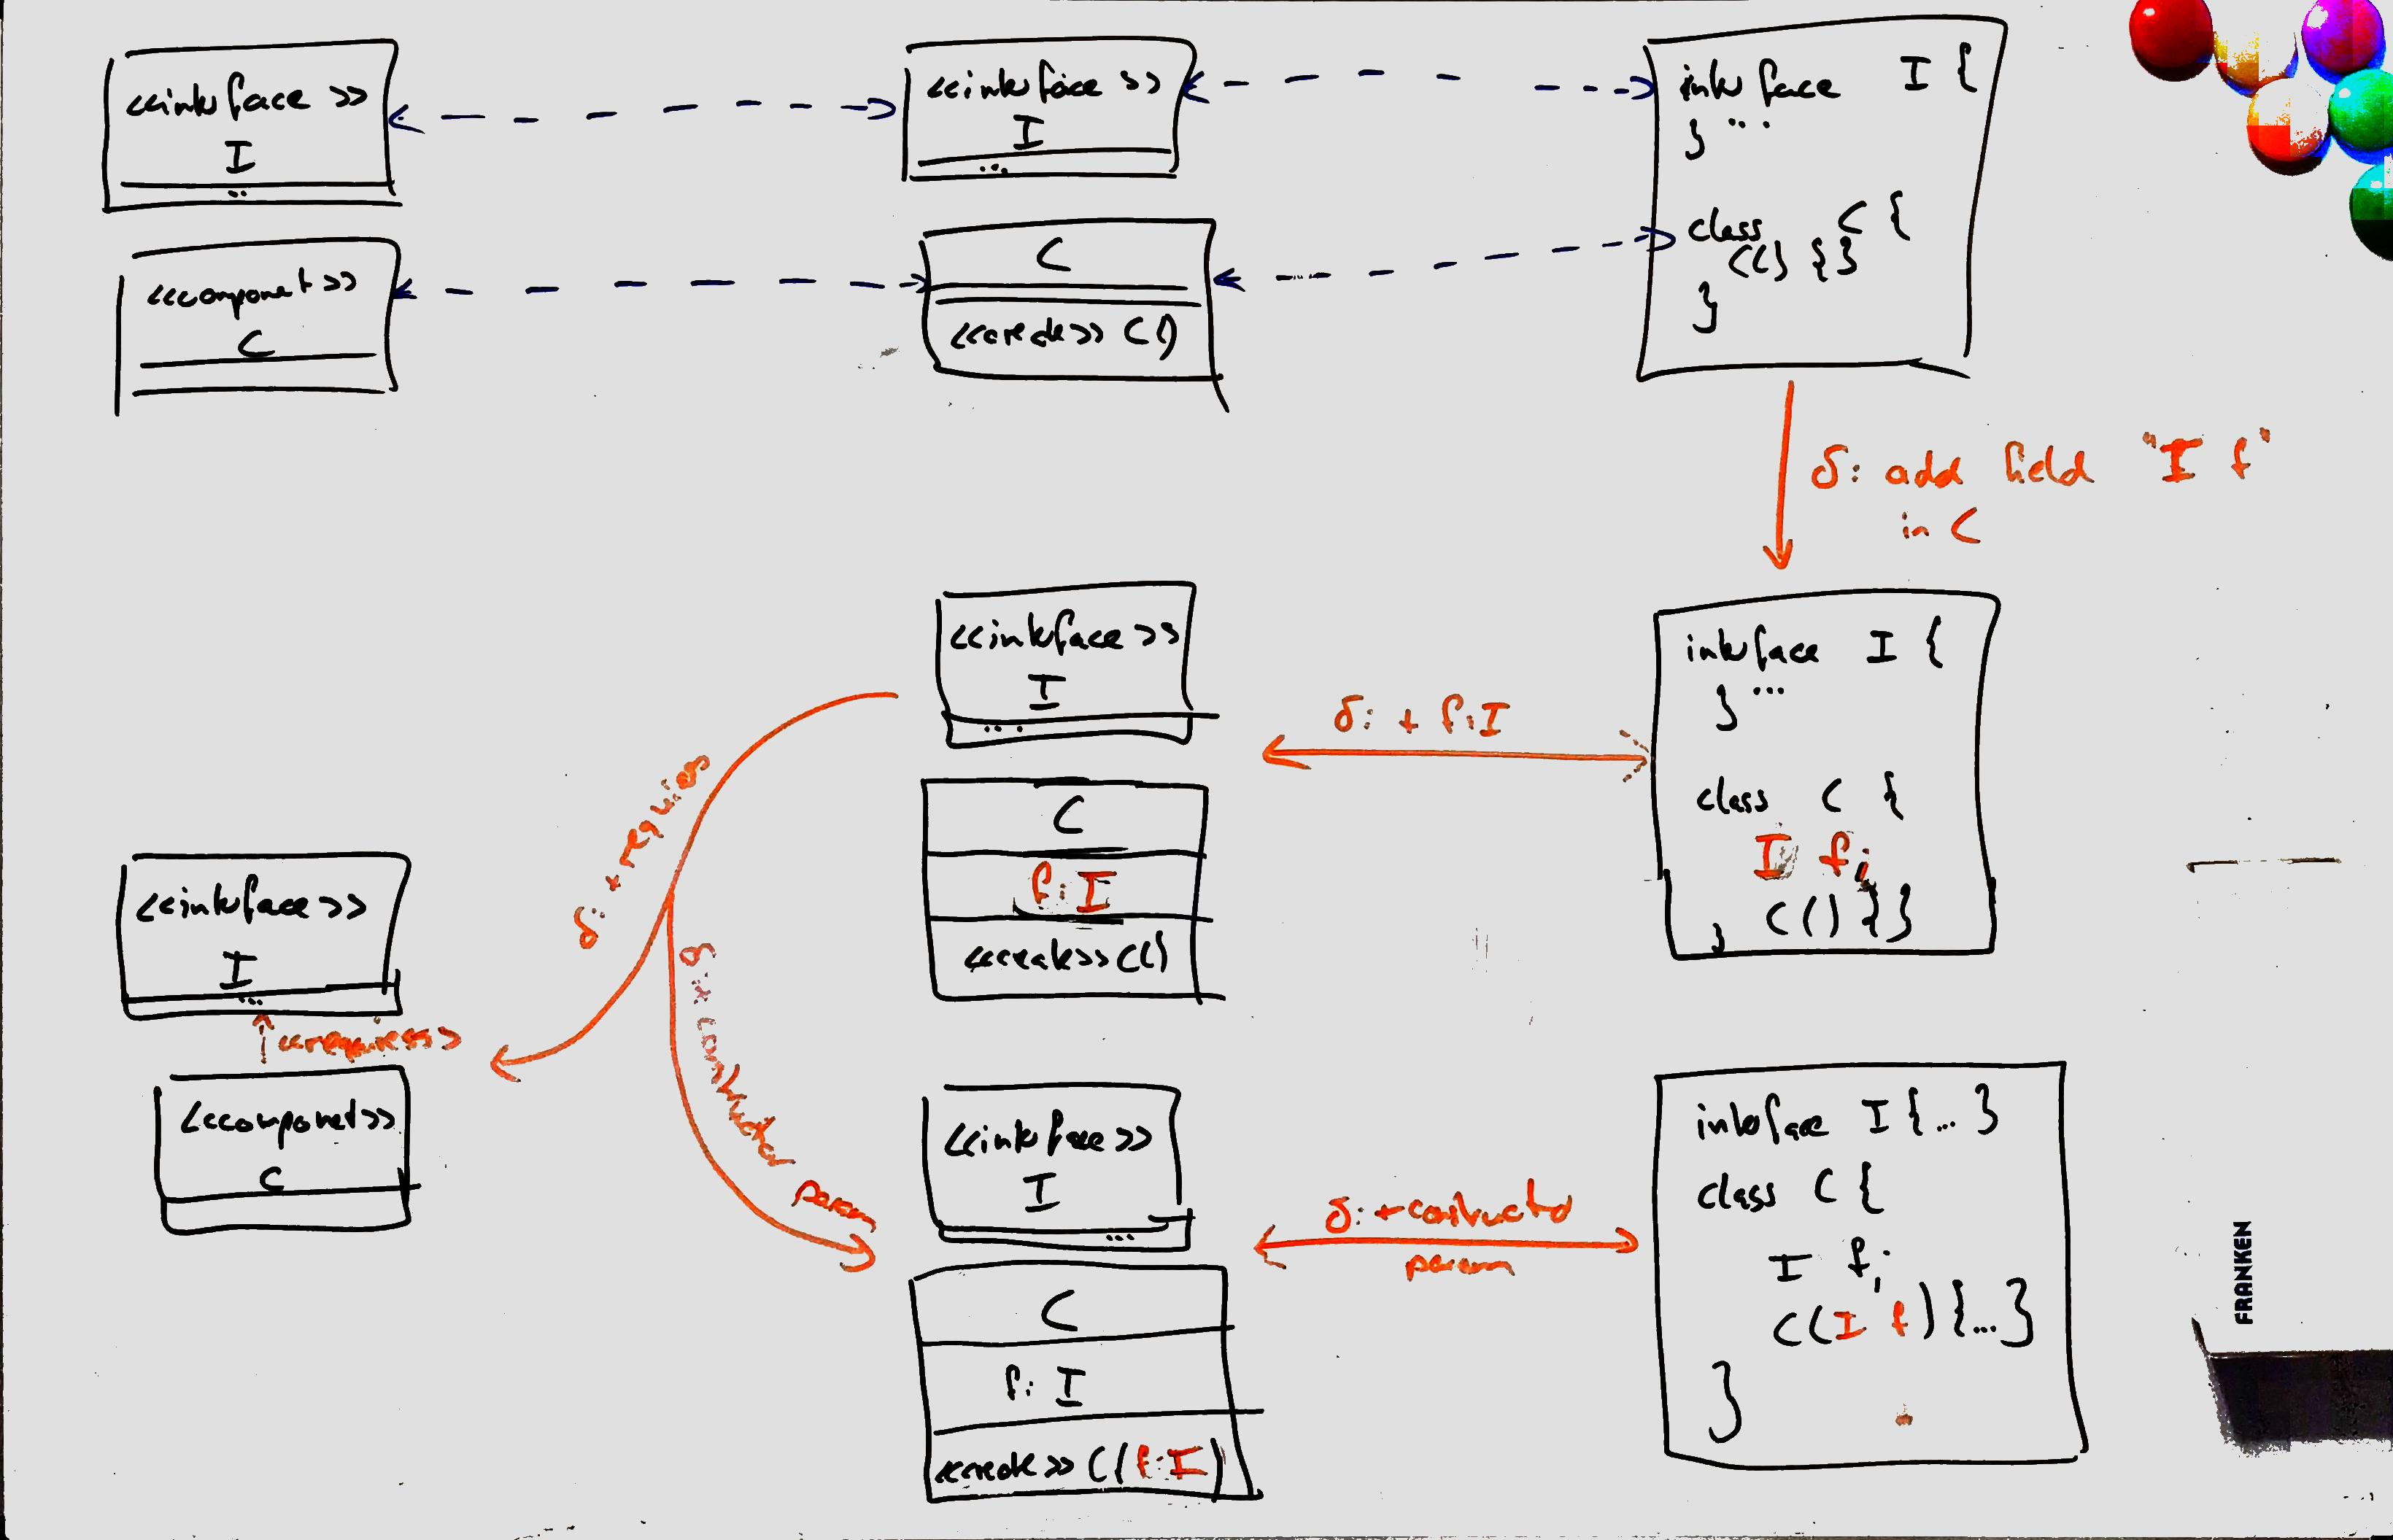
\includegraphics[width=\textwidth]{figures/correctness/orchestration/necessity_multiple_executions.jpg}
    \caption[Necessity of executing a transformation multiple times]{Necessity of executing a transformation multiple times.}
    \label{fig:orchestration:necessity_multiple_executions}
\end{figure}

\mnote{Example for component requires relation between \gls{PCM}, UML and Java}
Consider the example in \autoref{fig:orchestration:necessity_multiple_executions}, which describes the example depicted in \autoref{fig:introduction:scenario_duplicate_execution} within the introduction more precisely.
In the example, interfaces in UML and Java are related to architectural interfaces in a \gls{PCM} model.
\gls{PCM} components are realized by equally named classes in UML and Java.
Additionally, when a \gls{PCM} component requires an interface, this is realized by a field with the interface type in the component-realization class in UML and Java and an appropriate constructor argument.
Consistency is defined by transformations between \gls{PCM} and UML, as well as between UML and Java.

\mnote{Scenario requiring duplicate execution of one transformation}
In the scenario in \autoref{fig:orchestration:necessity_multiple_executions}, we begin with a consistent state of one interface and component, each realized by an interface and class, respectively, in both UML and Java.
A user then introduces a change of the Java code, in which he adds a field of the interface type to the component-realization class in Java.
The transformation between UML and Java propagates this change to the UML model, such that both models are consistent again.
The transformation between \gls{PCM} and UML then detects that the added field is of the type of an architectural interface, thus representing a requires relation between the corresponding component and the architectural interface. 
It adds the appropriate requires relation in the \gls{PCM} model, but also adds an appropriate parameter to the constructor of the component-realization class in UML, as required by the consistency relations.
This introduces a further inconsistency between the UML and the Java model, which requires the transformation between UML and Java to be executed again to also add that constructor parameter in the Java code.

\mnote{Cycles in transformation networks do not reduce necessary number of executions}
We simplified the example to the necessary core, although in practice a further transformation between \gls{PCM} and Java would be required, for example, to ensure that the field is set within the constructor.
One might argue that having a cycle of transformations between \gls{PCM}, UML and Java could resolve the problem, as the necessary second execution of the transformation between UML and Java is not necessary if the information is propagated from \gls{PCM} to Java.
This is, however, only true if exactly that order of transformations is chosen for execution and if the transformation between \gls{PCM} and Java does not introduce further information in the Java model that then needs to be propagated to UML.

\mnote{Synchronizing transformations can change models already processed by other transformation}
In general, it is always possible that transformations need to react to the changes performed by other, if they are not in some way aligned to each other.
This is due to the fact that a synchronizing transformation may change both models, thus if one transformation restores consistency between two models and another transformation reacts to that by restoring consistency between one of these models and another one, then both these models become changes, thus requiring the first transformation to process the newly created changes again.

\begin{figure}
    \centering
    \includegraphics[width=\textwidth]{figures/correctness/orchestration/no_upper_bound_example.png}
    \caption[Example for arbitrary bounds of transformation execution]{Example for an arbitrary bound of necessary transformation execution depending on value of $x$.}
    \todo{Ist das b.n-1 zwischen B und C in der Relation richtig? Das muss doch weg?}
    \label{fig:orchestration:no_upper_bound}
\end{figure}

\mnote{Generalization to a theoretical incrementation example}
We can generalize the previous example to the one given in \autoref{fig:orchestration:no_upper_bound}.
It is an extension of the example given in \autoref{fig:synchronization:multiple_unidirectional_execution} for the necessity to execute the consistency preservation rules of a bidirectional transformation multiple times.
This also applies to the case in which multiple bidirectional transformations are combined.
The depicted relations and the informally defined consistency preservation rules require that elements \modelelement{A}, \modelelement{B} and \modelelement{C} with the same value of $n$ exist, and that for each \modelelement{A} with value $n$ a \modelelement{B} and \modelelement{C} with $n$ incremented by $1$ exist, except for the case that $n = x-1$.
In consequence, for an \modelelement{A} with $n = i$, all \modelelement{A}, \modelelement{B} and \modelelement{C} with $i \leq n < x$ need to exist.
This, obviously, requires the transformations to be executed $x-1-i$ times.

\mnote{Precise definition of transformation network}
We prove the informally given statement with the following precise definition of the transformations for a variable value of $x$.
Let $\class{A}{}, \class{B}{}, \class{C}{}$ be the classes depicted in \autoref{fig:orchestration:necessity_multiple_executions}.
\begin{align*}
    & 
    \metamodelinstanceset{M}{1} = \mathcal{P}(\instances{\class{A}{}}), %\\
    %& 
    \metamodelinstanceset{M}{2} = \mathcal{P}(\instances{\class{B}{}}), %\\
    %& 
    \metamodelinstanceset{M}{3} = \mathcal{P}(\instances{\class{C}{}}) \\[1em]
    &
    \consistencyrelation{CR}{12} = \setted{\tupled{a,b} \in \instances{\class{A}{}} \times \instances{\class{B}{}} \mid b.n = a.n + 1 \neq x}, \consistencyrelationset{CR}_{12} = \setted{\consistencyrelation{CR}{12}, \consistencyrelation{CR}{12}^T} \\
    &
    \consistencypreservationrule{\consistencyrelationset{CR}_{12}}^{\rightarrow}(\model{m}{1}, \model{m}{2}, \change{\metamodel{M}{1}}) = \change{\metamodel{M}{2}} \\
    & \formulaskip
    \withmath \change{\metamodel{M}{2}}(\model{m}{2}) = \setted{b \in \instances{\class{B}{}} \mid \exists a \in \change{\metamodel{M}{1}}(\model{m}{1}) : b.n = a.n + 1 \neq x} \\
    & 
    \consistencypreservationrule{\consistencyrelationset{CR}_{12}}^{\leftarrow}(\model{m}{2}, \model{m}{1}, \change{\metamodel{M}{2}}) = \change{\metamodel{M}{1}} \\
    & \formulaskip
    \withmath \change{\metamodel{M}{1}}(\model{m}{1}) = \setted{a \in \instances{\class{A}{}} \mid \exists b \in \change{\metamodel{M}{2}}(\model{m}{2}) : b.n = a.n + 1 \neq x \land a \geq 0} \\
    &
    \transformation{t}_{12} = \tupled{\consistencyrelationset{CR}_{12}, \consistencypreservationrule{\consistencyrelationset{CR}_{12}}^{\rightarrow}, \consistencypreservationrule{\consistencyrelationset{CR}_{12}}^{\leftarrow}} \\[1em]
    & 
    \consistencyrelation{CR}{13} = \setted{\tupled{a,c} \in \instances{\class{A}{}} \times \instances{\class{C}{}} \mid c.n = a.n}, \consistencyrelationset{CR}_{13} = \setted{\consistencyrelation{CR}{13}, \consistencyrelation{CR}{13}^T} \\
    & 
    \consistencypreservationrule{\consistencyrelationset{CR}_{13}}^{\rightarrow}(\model{m}{1}, \model{m}{3}, \change{\metamodel{M}{1}}) = \change{\metamodel{M}{3}} \\
    & \formulaskip
    \withmath \change{\metamodel{M}{3}}(\model{m}{3}) = \setted{c \in \instances{\class{C}{}} \mid \exists a \in \change{\metamodel{M}{1}}(\model{m}{1}) : c.n = a.n} \\
    & 
    \consistencypreservationrule{\consistencyrelationset{CR}_{13}}^{\leftarrow}(\model{m}{3}, \model{m}{1}, \change{\metamodel{M}{3}}) = \change{\metamodel{M}{1}} \\
    & \formulaskip
    \withmath \change{\metamodel{M}{1}}(\model{m}{1}) = \setted{a \in \instances{\class{A}{}} \mid \exists c \in \change{\metamodel{M}{3}}(\model{m}{3}) : c.n = a.n} \\
    & 
    \transformation{t}_{13} = \tupled{\consistencyrelationset{CR}_{13}, \consistencypreservationrule{\consistencyrelationset{CR}_{13}}^{\rightarrow}, \consistencypreservationrule{\consistencyrelationset{CR}_{13}}^{\leftarrow}} \\[1em]
    &
    \consistencyrelation{CR}{23} = \setted{\tupled{b,c} \in \instances{\class{B}{}} \times \instances{\class{C}{}} \mid c.n = b.n}, \consistencyrelationset{CR}_{23} = \setted{\consistencyrelation{CR}{23}, \consistencyrelation{CR}{23}^T} \\
    & 
    \consistencypreservationrule{\consistencyrelationset{CR}_{23}}^{\rightarrow}, \consistencypreservationrule{\consistencyrelationset{CR}_{23}}^{\leftarrow} \andmath \transformation{t}_{23} \mathtextspacearound{accordingly} \\[1em]
    &
    \consistencyrelationset{CR} = \consistencyrelationset{CR}_{12} \cup \consistencyrelationset{CR}_{13} \cup \consistencyrelationset{CR}_{23} \\
    &
    \transformationset{T}_{inc} = \setted{\transformation{t}_{12}, \transformation{t}_{13}, \transformation{t}_{23}}
\end{align*}

\mnote{Proof that single execution of each transformation is not sufficient in scenario}
For these transformations, we are able to show that the transformation $\transformation{t}_{12}$ needs to be executed a minimal number of depending on $x$ for a specific input.
Thus, it is not sufficient to execute each transformation only once in this network.

\begin{lemma}[Minimal Number of Transformation Executions]
    \label{lemma:minimal_executions}
    Let $\transformationset{T}_{inc}$ be the previously defined set of transformations and let $\model{m}{1} = \model{m}{2} = \model{m}{3} = \emptyset$ be empty models and $\change{\metamodel{M}{1}} \in \changeuniverse{\metamodel{M}{1}}$ a change with $\change{\metamodel{M}{1}}(\model{m}{1}) = \setted{a \in \instances{\class{A}{}} \mid a.n = 0}$.
    Then the result of every orchestration function $\orcfunction{\transformationset{T}_{inc}}$ with $\appfunction{\orcfunction{\transformationset{T}_{inc}}}(\tupled{\model{m}{1},\model{m}{2},\model{m}{3}},\tupled{\change{\metamodel{M}{1}},\identitychange,\identitychange}) \consistenttomath \consistencyrelationset{CR}$ contains $\transformation{t}_{12}$ at least $x-1$ times.
\end{lemma}
\begin{proof}
    $\appfunction{\orcfunction{\transformationset{T}_{inc}}}$ can only return consistent models when it applies the transformations in the order delivered by $\orcfunction{\transformationset{T}_{inc}}$ by definition in \autoref{def:applicationfunction}.
    We thus consider any order of transformations, as delivered by any orchestration function, to show that it contains $\transformation{t}_{12}$ at least $x-1$ times to deliver consistent models.
    
    Let $max_n(\model{m}{1},\model{m}{2},\model{m}{3}) = max\setted{e.n \mid e \in \model{m}{1} \cup \model{m}{2} \cup \model{m}{3}}$ be the maximal value of $n$ in any instance of \modelelement{A}, \modelelement{B} and \modelelement{C} in any given models $\model{m}{1}$, $\model{m}{2}$ and $\model{m}{3}$. In the following, we shortly note $max_n$ if the concrete models are currently not relevant.

    \begin{properdescription}
        \item[Executing $\transformation{t}_{13}$ and $\transformation{t}_{23}$ an arbitrary number of times does not increase $max_n$:]
        The transformations do only ensure that for any given models the returned models contain all elements with the same values of $n$ and do not introduce new elements with values of $n$ larger than the existing ones.
        \item[A single execution of $\transformation{t}_{12}$ increases $max_n$ by at most one:]
        There is no \modelelement{A} or \modelelement{B} with $n > max_n$.
        For every \modelelement{A} with $n < max_n$, $\transformation{t}_{12}$ creates, if necessary, a \modelelement{B} with value $n + 1 \leq max_n$, thus not increasing $max_n$.
        For every \modelelement{B} with $n \leq max_n$, it creates, if necessary, an \modelelement{A} with value $n-1 < max_n$.
        For every \modelelement{A} with $n = max_n$, a \modelelement{B} with value $n+1 = max_n + 1$ is creates, as long as $n \neq x-1$.
        For the newly created \modelelement{B}, no further elements needs to be created to fulfill the consistency relations.
        Thus, $max_n$ is, at most, increased by $1$.
        \item[ When $max_n(\model{m}{1},\model{m}{2},\model{m}{3}) < x-1$, then $\model{m}{1},\model{m}{2},\model{m}{3}$ are not consistent to $\consistencyrelationset{CR}$:]
        There is at least one element within the models with $n = max_n$.
        If the element with $n = max_n$ is an \modelelement{A}, then there must be a \modelelement{B} with value $n+1$, because of $\consistencyrelationset{CR}_{12}$ and because $n < x-1$.
        But since $n = max_n$, such a \modelelement{B} cannot exist, because otherwise $max_n = n+1$, so this is a contradiction.    
        If the element with $n = max_n$ is a \modelelement{C}, then $\consistencyrelationset{CR}_{13}$ requires an \modelelement{A} with the same value of $n$ to exist and the same argument as before leads to a contradiction.
        Finally, if the element with $n = max_n$ is a \modelelement{B}, then because of $\consistencyrelationset{CR}_{23}$ a \modelelement{C} with the same value must exist and then the same argument as before leads to a contradiction.
    \end{properdescription}

    In summary, we have shown that models $\model{m}{1},\model{m}{2},\model{m}{3}$ are only consistent to $\consistencyrelationset{CR}$ when $max_n(\model{m}{1},\model{m}{2},\model{m}{3}) \geq x-1$.
    Additionally, only $\transformation{t}_{12}$ increases $max_n$ and with each execution it only increases it by at most $1$.
    In consequence, starting with $max_n = 0$, we need at least $x-1$ executions of $\transformation{t}_{12}$ in an arbitrary sequence of the transformations in $\transformationset{T}_{inc}$ to achieve consistent models.
\end{proof}

\mnote{Example transformations can force network to perform an arbitrary number of executions}
We have proven that arbitrary transformation networks can require an arbitrary high number of executions of each transformations.
By selecting an appropriate $x$ in the used example network, we can force the network to perform at least $x$ executions of one transformation to yield a consistent tuple of models.
With this insight, it directly follows that we cannot find an approach to define orchestration functions that delivers sequences containing each transformation only once if we want to ensure that if a consistent orchestration of transformations exists, the approach is supposed to deliver it.

\begin{theorem}[Orchestration with Single Execution]
    \label{theorem:orchestration_single}
    For any set of transformations $\transformationset{T}$, there can be models $\modeltuple{m}$ and changes $\changetuple{}$ to them for which each possible orchestration function $\orcfunction{\transformationset{T}}$ with whom $\appfunction{\orcfunction{\transformationset{T}}}(\modeltuple{m}, \changetuple{})$ is consistent, delivers a sequence as $\orcfunction{\transformationset{T}}(\modeltuple{m}, \changetuple{})$ that contains at least one transformation twice.
\end{theorem}
\begin{proof}
    We know from \autoref{lemma:minimal_executions} that $\transformationset{T}_{inc}$ requires at least $2$ executions of $\transformation{t}_{12}$ for the inputs defined in \autoref{lemma:minimal_executions} when selecting $x \geq 3$.
    This proves the theorem by example.
\end{proof}

\mnote{Example generalizes practical scenario, thus single execution not supposed to be sufficient}
We know from \autoref{theorem:orchestration_single} that if we execute each transformation only once, we may exclude cases for which multiple executions of transformations would have led to a consistent tuple of models.
The example we have given in \autoref{fig:orchestration:necessity_multiple_executions} is a simplification of a realistic transformation scenario, which we generalized to the previous network with transformations $\transformationset{T}_{inc}$.
Thus, we can conclude that the insight is potentially relevant for realistic scenarios.
We should not restrict orchestration to execute each transformation only once, as there can be realistic scenarios in which multiple executions are necessary to find consistent models.
In the following, we thus, for first, allow an arbitrary number of executions of each transformation.

% Essential problem: One transformation may restore consistency between A and B and another between A and C. If then a transformation restores consistency between B and C, the resulting B' and C' may not be consistent A anymore.

% \todo{Beispiel warum mehrfache Ausführung nötig, warum also manche Infos erst durch andere bx reinkommen, die bei einer bx isoliert nicht relevant sind.}

% Bestehende Arbeiten (\cite{stevens2020BidirectionalTransformationLarge-SoSym}) schlagen auch vor eine Baumstruktur zu berechnen (Spannbaum), in dem nur entlang der Baumkanten die Transformationen ausgeführt werden. Dies ist jedoch eine starke Einschränkung daran, was die Transformationen ausdrücken können. Betrachtet man beispielsweise PCM, UML und Java, und hat eine Änderung in PCM. Dann könnte der Spannbaum entweder PCM -> UML -> Java sein, oder PCM -> UML + PCM -> Java. In ersterem Fall würde Verhaltensbeschreibung, die von PCM nach Java übertragen, aber in UML nicht dargestellt wird, nicht übertragen. Im zweiten Fall würde zusätzliche Information zwischen UML und Java nicht propagiert (Beispiel?) --> Hier sollte auf das Properties-Kapitel verwiesen werden, wo diese "Bottlenecks" erklärt sein sollten, inklusive einem Beispiel, die allgemein Baumstrukturen für Transformationsnetwerke ausschließen.

% Consequence: We cannot easily restrict the number of allowed executions. We can define networks that require an arbitrary number of executions.
% Also refer to the synchronization example, where we discussed that.
% Let us, for first, assume that transformations need an arbitrary number of executions.


\subsection{Orchestration Function Behavior} %The Orchestration Problem %Expected Behavior} % Failure Cases} %When to Return $\bot$?}
\label{chap:orchestration:problem:function_behavior}

\mnote{Necessity to define when application function returns $\bot$}
The application function is defined to return models only when they can be derived by applying transformations in an order delivered by the orchestration function and otherwise to return $\bot$.
In addition, we expect a \emph{correct} application function only to deliver models that are consistent.
We did, however, not yet define under which conditions we expect the function not to return $\bot$, because there are different reasons why the function may not be able to deliver consistent models although we could expect it to do so.
In fact, with the current definition, the function is even considered correct if it always returns $\bot$, which is not practical.
Thus, we need to define when exactly we expect the function to return $\bot$.

\mnote{Reasons for not finding an orchestration that yields consistent models}
It might be intuitive to expect an application function to always return consistent models when the input models are consistent and when there is an execution order of the transformations, i.e., an orchestration, that delivers consistent models.
This, in consequence, would lead to the requirement that the orchestration function delivers a sequence of transformations whose application delivers consistent models whenever such a sequence exists for the given models and changes to them.
There can be different reasons why the orchestration function may not deliver such a sequence:
%When is it allowed or needed to return $\bot$?
%It may always return $\bot$ to be correct, this is however not what we want.
%We can distinguish three levels of reasons why the function may not be able to find consistent models:
\begin{properdescription}
    \item[Relations are incompatible:] If the consistency relations are incompatible, a user change may introduce an element for which no consistent models exist. In consequence, the transformation cannot be executed in an order such that the resulting models are consistent and still reflect the given user change.
    %(example with employee for which no consistent other models can be found)
    \item[No orchestration exists:] Even if the relations are compatible, transformations may be defined in a way that they make contradictory decisions for locally consistent solutions. Thus, for a given a change the consistency relations allow different ways to store consistency, of which the transformations always select a way that is not consistent to one of the other relations.
    Then no order of the transformations can restore consistency, although models exist that fulfill consistency for the given change.
    % (example with three options for name mapping with one overlapping, where each transformation always selects the one that is not appropriate for the other). We can further distinguish here whether there is always a change that cannot be processed by a CPR (then the change conflicts with the consistency relations and thus has to be rejected like any change may need to be rejected), or whether an arbitrary long sequence of transformations exists that can be applied but does never yield a consistent set of models.
    \item[No orchestration found:] Finally, although an order of transformations for given changes exists that delivers consistent models, the orchestration function may not deliver it. 
    %finally, the application/orchestration may not be able to find an order of transformations that leads to a consistent state although it exists.
\end{properdescription}

\mnote{Reasons form an induction hierarchy}
These reasons can be considered at different levels, because each of them induces the next, i.e., if there is no orchestration, it cannot be found, and having contradictory relations, there exists no orchestration for some of the changes.
In the end, all of them lead to the situation that no orchestration can be found and, thus, the orchestration function is not able to deliver it.

\mnote{Compatibility can be assumed, existence of an orchestration cannot}
The initially given intuitive requirement that the orchestration function delivers a consistent orchestration whenever it exists would thus assume that the first two levels do not occur and then require the orchestration function to ensure the third.
While we can assume compatibility of the relations, as we discussed how to analyze it in \autoref{chap:compatibility}, we cannot assume that an orchestration does always exists, as we will see in the following.

\mnote{Compatibility does not ensure existence of orchestration}
Although compatibility reduces the chance that an orchestration function does not deliver a consistent orchestration, as we have motivated with the scenario depicted in \autoref{fig:compatibility:unwanted_behavior}, it does not ensure that there is always such a sequence of transformations that the orchestration function can find.
In general, this is always the case when consistency relations define different options for consistency, i.e., they allow the existence of different corresponding elements to consider the models consistent.
Compatibility ensures that there is an overlap of these corresponding elements, such that for every element, for which consistency is restricted, consistent models can be found.
If, however, the consistency preservation rules of the transformations always restore consistency by introducing corresponding elements that are not in this overlap, each transformation will restore consistency locally to its consistency relation, but they can, together, never restore consistency to all consistency relations.

\mnote{Consistency preservation rules need to select overlapping options in consistency relations}
Consider the situation that we have three metamodels $\metamodel{A}{}$, $\metamodel{B}{}$ and $\metamodel{C}{}$ with instances $\model{a}{i}$, $\model{b}{i}$ and $\model{c}{i}$.
Let us assume that those models are uniquely indexed by $i$ and we defined the following consistency relations:
\begin{align*}
    &
    \consistencyrelation{CR}{AB} = \setted{\tupled{\model{a}{i}, \model{b}{k}} \mid k = i} \\
    &
    \consistencyrelation{CR}{AC} = \setted{\tupled{\model{a}{i}, \model{c}{l}} \mid l = i \lor l = i+1} \\
    &
    \consistencyrelation{CR}{BC} = \setted{\tupled{\model{b}{k}, \model{c}{l}} \mid l = k+1 \lor l = k+2}
\end{align*}
This induces the set of consistent model tuples $\setted{\tupled{\model{a}{i}, \model{b}{k}, \model{c}{l}} \mid  i = k = l-1}$, which is given to all three consistency relations.
Thus for any given model we are able to find instances of the other metamodels that are consistent to all consistency relations.
If we define consistency preservation rules for these consistency relations, the ones for $\consistencyrelation{CR}{AC}$ and $\consistencyrelation{CR}{BC}$ may decide between two models to restore consistency.
If $\consistencyrelation{CR}{AC}$ does always select $\model{c}{i}$ for $\model{a}{i}$ and vice versa, and if $\consistencyrelation{CR}{BC}$ does always select $\model{c}{i+2}$ for $\model{a}{i}$ and vice versa, no orchestration of the transformations will yield consistent models, because they never select those models that are in the overlap of the consistency relations.

\begin{figure}
    \centering
    \includegraphics[width=\textwidth]{figures/correctness/orchestration/no_orchestration.png}
    \caption[Consistency preservation rules without orchestration]{Consistency relations with options for corresponding elements leading to consistency preservation rules for which no consistent orchestration exists.}
    \label{fig:orchestration:no_orchestration}
\end{figure}

\mnote{Running example with consistency relations for name composition}
We have already given an abstract example for that problem in \autoref{fig:correctness:no_execution_order}. \autoref{fig:orchestration:no_orchestration}, in addition, demonstrates this situation at a derivation of the running example.
The consistency relation between employees and residents ensures that for each resident and employee there is corresponding other element with the same name.
The consistency relations between employees and persons and between residents and persons ensure that for each person there is a corresponding employee and resident, respectively, but they allow different relations of their names.
While both consider elements corresponding if the name of an employee and resident, respectively, are the concatenation of the first and last name of a person, an employee is also allowed to have the inverse concatenation of last and first name, whereas a resident is also allowed to have this inverse concatenation, but with an additional separation of the last and first name with a comma.
These options for the consistency relations provide further degrees of freedom for each transformation on its own, as they allow, for example, employee names to be encoded differently.
This can, for example, be reasonable if the order of first and last name is not relevant in a model managing employees.
In combination with the other consistency relations, however, the only employees, residents and persons that are considered consistent to all of the consistency relations are those having the same names with the concatenation of first and last name.
Nevertheless, these consistency relations are compatible, because for each possible condition element, i.e., for every possible employee, person and resident, there are consistent models that contain them.

\mnote{Relations in the running example without consistent orchestration}
Consistency relations that preserve these consistency relations need to to choose one of the given options for the names of corresponding employees, residents and persons.
\autoref{fig:orchestration:no_orchestration} sketches consistency preservation rules that make such a selection.
The rules with alternative 1 ensure that for each employee, resident and persons corresponding elements exist, which fulfill those relations of the names that are conflicting.
This means, the employee name is the concatenation of the last and first name of a person, whereas the resident name contains an additional comma in that concatenation.
In the other direction, the names of employees and residents are split at the appropriate indices, given by the whitespace and comma, respectively, to calculate the required first and last name of a person.
In consequence, there is no execution sequence of the transformations that results in consistent models, because the execution of the transformation between employees and persons always leads to a violation of the consistency relation between residents and persons and vice versa.
This is because the transformation between person and resident always introduces a comma in the resident name, which is then appended to the last name by the transformation between employee and persons.
A repeated execution of the transformation repeatedly appends that comma.
On the other hand, the execution of any of the transformation does never lead to the introduction of a person that fulfills the non-conflicting conditions of both consistency relations by simply containing a first and last name, which is represented as concatenation of first and last name in both an employee and resident.
This is concrete example for the previously discussed abstract situation that of different options in consistency relations always the non-overlapping ones are chosen by the consistency preservation rules.

\mnote{Alternative relations in the running example}
If we consider the alternative 2 for the consistency preservation rule between persons and residents, we can always find a consistent orchestration.
The alternative rule decides how consistency is ensured based on the existence of a comma within the resident name.
If a comma is present, the name relation containing a comma is used, and otherwise the simple concatenation of first and last name is assumed.
For an employee, first execution the transformation from employees to residents and afterwards the one from residents to persons ensures that all consistency relations are fulfilled, because the one between residents and persons sets first and last name of a person according to the relations that is also fulfilled between person and employee, because the name does not contain a comma.
For a person, first executing the transformation from persons to employees and then following the process above also ensures consistency.
Finally, for a resident, we can, for example, first apply the transformation between residents and employees and then the one between residents and persons, resulting in consistent models due to the same reasons as above.

\mnote{Only specific orchestrations yield consistent models}
Although there are consistent orchestration of the transformations with the consistency preservation rule defined as alternative 2, not every execution order leads to consistent models.
In the scenarios discussed above, we have ensured that the transformation between residents and persons is executed for a resident first.
If that transformation is first executed for a person, then a comma is added, which leads to the subsequent application of the same consistency preservation rules as with alternative 1, meaning that no further orchestration yields consistent models.

\mnote{Necessity to find consistent orchestrations}
No matter whether exactly those consistency relations and preservation rules for them may occur in an actual transformation network, they exemplify the general situation of having consistency preservation rules that select one of different options provided by the consistency relation to introduced corresponding elements to restore consistency.
The example shows that whether or not a consistent orchestration of transformations exists in such a situation depends on whether at least one transformation selects an option that is consistent to other consistency relations as well.
It also shows that even if a consistent orchestration exists, not all orchestrations yield consistent models, thus we need to be able to find one that does.

\mnote{Resolvability as the existence of an orchestration}
In accordance with existing work \cite{stevens2020BidirectionalTransformationLarge-SoSym}, we call a given tuple of models and changes \emph{resolvable} by a transformation network, if an orchestration exists.
In contrast to existing work, we do, however, not restrict ourselves to a single execution of each transformation, as we have motivated before.

\mnote{Necessity to deal with unresolvability}
We have to accept that transformation networks may be unresolvable, i.e., that there is no consistent orchestration of the transformations.
Ensuring that a network is resolvable for any changes would lead to restrictions for the individual transformations, which would especially require different transformations to be aligned with each other.
Since that conflicts our assumption of independent development and modular reuse, we do not focus on that problem, but accept that it can occur and instead focus on how we can find an orchestration if it exists. 

\mnote{Optimality property of orchestration function}
In conclusion, we expect the application function to deliver consistent models whenever a consistent orchestration, i.e., an execution order that yields consistent models, exists.
Thus, we want to ensure that the orchestration function is able to always find such an orchestration, if it exists.
We define this as an \emph{optimality} property in the following.

% "has a resolution" bei Stevens entspricht im Prinzip Kompatibilität
% "is resolvable" bei Stevens entspricht im Prinzip "orchestration exists"

% In accordance to existing work, such as \cite{stevens2020BidirectionalTransformationLarge-SoSym}, we call a given set of models and changes \emph{resolvable} by the transformation network, if there exists a sequence of the transformations such that the resulting models are consistent.
% We do, however, not restrict ourselves to a single execution of each transformation but allow them to be executed multiple times (as motivated before).
% Orchestration ermittelt eine "Resolution" (siehe bestehende Arbeiten~\cite{stevens2020BidirectionalTransformationLarge-SoSym}), also eine Ausführungsreihenfolge, zumindest wenn man sie als "korrekt" bezeichnet.

% Argumentation:
% Compatibility können wir fordern, dass eine Orchestrierungsstrategie existiert aber nicht. 

% We can avoid the first by requiring compatibility.
% We need to make restrictions to the transformation to resolve the second. We do, however, probably need to require them to know about the other transformations to avoid that. Finally, we will have to deal with that situation and then inform the user about the problem.
% We investigate whether we can always guarantee to find an orchestration if it exists.
% For now, we focus on the last problem, since that is a problem of the application and orchestration function, rather than the problem that no orchestration may exist at all.

% DECIDED THAT THE FOLLOWING IS NOT AN OPTINO BUT THE SECOND IS DEFINITE.
% Now we have these options:
% \begin{itemize}
%     \item We accept that there is no orchestration or that the strategy does not find it in specific situations, than we only need to consider that the strategy must always terminate.
%     We could, for example, change the algorithm such that it always returns $\bot$, which is correct, or terminates after executing each transformation once.
%     \item We define a precise criterion when the strategy is allowed to return $\bot$. Most intuitively, one might say that it should only return $\bot$ whenever no orchestration exists.
% \end{itemize}



\subsection{Optimal Orchestration}

% An application function that delivers consistent models whenever an orchestration exists that yields them is what we would assume \emph{optimal}.
% Recall that $\generalizationfunction{\metamodeltuple{M},\transformation{t}}$ is the generalization function that applies a transformation, which is only defined for two models, to a model tuple that instantiate all metamodels in $\metamodeltuple{M}$.

% \begin{definition}[Optimal Transformation Application Function]
%     Let $\transformationset{T}$ be a set of transformations for a set of metamodels $\metamodeltuple{M} = \tupled{\metamodelsequence{M}{n}}$.
%     We say that an application function $\appfunction{\orcfunction{\transformationset{T}}}$ for these transformations is \emph{optimal} if it returns models that are consistent whenever there is an orchestration of the transformation that yields a consistent set of models whenever it exists, i.e.,
%     \begin{align*}
%         &
%         \forall \modeltuple{m} \in \metamodeltupleinstanceset{M} : \forall \changetuple{\metamodeltuple{M}} = \tupled{\change{\metamodel{M}{1}}, \dots, \change{\metamodel{M}{n}}} \in \changeuniverse{\metamodeltuple{M}} :
%         \modeltuple{m} \consistenttomath \consistencyrelationset{CR} \Rightarrow \\
%         & \formulaskip
%         \bigl(
%             \exists \transformation{t}_{1}, \dots, \transformation{t}_{m} \in \transformationset{} : 
%             \exists \changetuple{\metamodeltuple{M}}' = \tupled{\change{\metamodel{M}{1}}', \dots, \change{\metamodel{M}{n}}'} \in \changeuniverse{\metamodeltuple{M}} :\\
%             & \formulaskip \formulaskip
%             \generalizationfunction{\metamodeltuple{M}, \transformation{t}_{1}} \concatfunction \dots \concatfunction \generalizationfunction{\metamodeltuple{M}, \transformation{t}_{m}}(\modeltuple{m}, \changetuple{\metamodeltuple{M}}) = (\modeltuple{m}, \changetuple{\metamodeltuple{M}}')\\
%             & \formulaskip \formulaskip
%             \land \tupled{\change{\metamodel{M}{1}}'(\model{m}{1}), \dots, \change{\metamodel{M}{n}}'(\model{m}{n})} \consistenttomath \consistencyrelationset{CR} \bigr) \\
%             & \formulaskip
%             \Rightarrow \appfunction{\orcfunction{\transformationset{T}}}(\modeltuple{m},\changetuple{\metamodeltuple{M}}) \consistenttomath \consistencyrelationset{CR}
%         \bigr)
%     \end{align*}
% \end{definition}

\mnote{Definition of optimal orchestration function}
To ensure that an application function delivers consistent models whenever a consistent orchestration exists, we need to find an orchestration function that fulfills this property.
We denote this as an \emph{optimal} orchestration function.
Recall that $\generalizationfunction{\metamodeltuple{M},\transformation{t}}$ is the generalization function that applies a transformation, which is only defined for two models, to a model tuple that instantiate all metamodels in $\metamodeltuple{M}$.
% It is obvious that we can define consistency preservation rules for which the orchestration function cannot find an execution order that returns a consistent tuple of models after certain changes. We already gave an example in \autoref{fig:correctness:no_execution_order}. There exists no execution order for any input value that terminates. The transformations will always increase the value, although the defined relations could be fulfilled for the input value, but the transformations never find that solution.

% Although we will discuss restrictions to relations and transformations that reduce the chance that no solution can be found, it will not be possible to ensure that such a solution can always be found. This is due to the reason that transformations can perform arbitrary changes given that transformations are Turing complete, which should not be restricted, because it is unclear which restrictions could be made without forbidding scenarios that should actually we supported. Thus, we assume that transformations are Turing complete.

% We explicitly allow the orchestration function to return a sequence that will, if applied to models and changes to them, not deliver a consistent tuple of models. As discusses, this is supposed to reflect cases in which no such sequence can be calculated.
% However, it may be useful to have some notion of \emph{optimality} that ensures that if a sequence that delivers a consistent result exists, the orchestration function is supposed to find it.
% Formally, this notion looks as follows.

\begin{definition}[Optimal Transformation Orchestration Function]
    Let $\transformationset{T}$ be a set of transformations for a tuple of metamodels $\metamodeltuple{M}% = \tupled{\metamodelsequence{M}{n}}
    $.
    We say that an orchestration function $\orcfunction{\transformationset{T}}$ for these transformations is \emph{optimal} if it returns a consistent orchestration whenever it exists, i.e.,
    \begin{align*}
        &
        \forall \modeltuple{m} \in \setted{\modeltuple{m}' \in \metamodeltupleinstanceset{M} \mid \modeltuple{m}' \consistenttomath \consistencyrelationset{CR}} : \forall \changetuple{\metamodeltuple{M}} %= \tupled{\change{\metamodel{M}{1}}, \dots, \change{\metamodel{M}{n}}} 
        \in \changeuniverse{\metamodeltuple{M}} : \\
        %\modeltuple{m} \consistenttomath \consistencyrelationset{CR} \Rightarrow \\
        & \formulaskip
        %\bigl[ 
            \bigl(
            \exists \transformation{t}_{1}, \dots, \transformation{t}_{i} \in \transformationset{T} : 
            \exists \changetuple{\metamodeltuple{M}}' %= \tupled{\change{\metamodel{M}{1}}', \dots, \change{\metamodel{M}{n}}'} 
            \in \changeuniverse{\metamodeltuple{M}} : \changetuple{\metamodeltuple{M}}'(\modeltuple{m})
            \consistenttomath \consistencyrelationset{CR}\\
            & \formulaskip \formulaskip
            \land \generalizationfunction{\metamodeltuple{M}, \transformation{t}_{1}} \concatfunction \dots \concatfunction \generalizationfunction{\metamodeltuple{M}, \transformation{t}_{i}}(\modeltuple{m}, \changetuple{\metamodeltuple{M}}) = (\modeltuple{m}, \changetuple{\metamodeltuple{M}}') %\bigr)
            \\
            % & \formulaskip \formulaskip
            %\land \changetuple{\metamodeltuple{M}}'(\modeltuple{m})
            %\tupled{\change{\metamodel{M}{1}}'(\model{m}{1}), \dots, \change{\metamodel{M}{n}}'(\model{m}{n})} 
            %\consistenttomath \consistencyrelationset{CR} \bigr) \\
            & \formulaskip
            \Rightarrow %\bigl(        
            \exists \transformation{t}_{1}', \dots, \transformation{t}_{k}' \in \transformationset{} : 
            \exists \changetuple{\metamodeltuple{M}}'' %= \tupled{\change{\metamodel{M}{1}}'', \dots, \change{\metamodel{M}{n}}''} 
            \in \changeuniverse{\metamodeltuple{M}} : \changetuple{\metamodeltuple{M}}''(\modeltuple{m}) \consistenttomath \consistencyrelationset{CR}\\
            & \formulaskip \formulaskip
            \land \orcfunction{\transformationset{T}}(\modeltuple{m}, \changetuple{\metamodeltuple{M}}) = \sequenced{\transformation{t}_{1}', \dots, \transformation{t}_{k}'} \\
            & \formulaskip \formulaskip
            \land \generalizationfunction{\metamodeltuple{M},\transformation{t}_{1}'} \concatfunction \dots \concatfunction \generalizationfunction{\metamodeltuple{M},\transformation{t}_{k}'}(\modeltuple{m}, \changetuple{\metamodeltuple{M}}) = (\modeltuple{m}, \changetuple{\metamodeltuple{M}}'') %\\
            % & \formulaskip \formulaskip
            % \land \changetuple{\metamodeltuple{M}}''(\modeltuple{m})
            % %\tupled{\change{\metamodel{M}{1}}''(\model{m}{1}), \dots, \change{\metamodel{M}{n}}''(\model{m}{n})} 
            % \consistenttomath \consistencyrelationset{CR}
        \bigr) %\bigr]
    \end{align*}
\end{definition}

\mnote{Optimal orchestration function not restricted to return sequence only when it yields consistent models}
Note that we do not require an optimal orchestration function not to return a sequence when there is no consistent orchestration.
This is reasonable, because an application function may be defined to return consistent models whenever there is a consistent orchestration, but to also support the process of identifying why there is none by delivering a sequence of transformations that leads to a failure.

\mnote{Optimality of the application function}
Finally, the result of the application function is what is relevant in the process of consistency preservation in a transformation network.
Thus, we apply the notion of \emph{optimality} to that function accordingly by requiring it to deliver consistent models whenever a consistent orchestration exists.

\begin{definition}[Optimal Transformation Application Function]
    \label{def:optimalapplicationfunction}
    Let $\transformationset{T}$ be a set of transformations for a tuple of metamodels $\metamodeltuple{M} %= \tupled{\metamodelsequence{M}{n}}
    $.
    We say that an application function $\appfunction{\orcfunction{\transformationset{T}}}$ for these transformations is \emph{optimal} if it returns models that are consistent whenever there is a consistent orchestration of the transformation, i.e.,
    \begin{align*}
        &
        \forall \modeltuple{m} \in \setted{\modeltuple{m}' \in \metamodeltupleinstanceset{M} \mid \modeltuple{m}' \consistenttomath \consistencyrelationset{CR}} : \forall \changetuple{\metamodeltuple{M}} %= \tupled{\change{\metamodel{M}{1}}, \dots, \change{\metamodel{M}{n}}} 
        \in \changeuniverse{\metamodeltuple{M}} : \\
        %\modeltuple{m} \consistenttomath \consistencyrelationset{CR} \Rightarrow \\
        & \formulaskip
        \bigl(
            \exists \transformation{t}_{1}, \dots, \transformation{t}_{m} \in \transformationset{T} : 
            \exists \changetuple{\metamodeltuple{M}}' %= \tupled{\change{\metamodel{M}{1}}', \dots, \change{\metamodel{M}{n}}'} 
            \in \changeuniverse{\metamodeltuple{M}} : \changetuple{\metamodeltuple{M}}'(\modeltuple{m}) \consistenttomath \consistencyrelationset{CR}\\
            & \formulaskip \formulaskip
            \land \generalizationfunction{\metamodeltuple{M}, \transformation{t}_{1}} \concatfunction \dots \concatfunction \generalizationfunction{\metamodeltuple{M}, \transformation{t}_{m}}(\modeltuple{m}, \changetuple{\metamodeltuple{M}}) = (\modeltuple{m}, \changetuple{\metamodeltuple{M}}') %\\
            %& \formulaskip \formulaskip
            %\land \tupled{\change{\metamodel{M}{1}}'(\model{m}{1}), \dots, \change{\metamodel{M}{n}}'(\model{m}{n})} \consistenttomath \consistencyrelationset{CR} 
            %\bigr) 
            \\
            & \formulaskip
            \Rightarrow \appfunction{\orcfunction{\transformationset{T}}}(\modeltuple{m},\changetuple{\metamodeltuple{M}}) \consistenttomath \consistencyrelationset{CR}
        \bigr)
    \end{align*}
\end{definition}

\mnote{Optimal application function requires optimal orchestration function}
According to the defined behavior of an application function, an optimal application function requires an optimal orchestration function.

\begin{lemma}[Application / Orchestration Function Optimality]
    \label{lemma:optimalapplicationfunction}
    An application function $\appfunction{\orcfunction{\transformationset{T}}}$ can only be optimal if $\orcfunction{\transformationset{T}}$ is optimal.
\end{lemma}
\begin{proof}
    Let us assume that the complete condition in \autoref{def:optimalapplicationfunction} is fulfilled, i.e., that the input models are consistent and that there is consistent orchestration of the transformations.
    Then to be optimal, the application function needs to return models that are consistent.
    According to the definition of an application function (see \autoref{def:applicationfunction}), the sequence of transformations delivered by $\orcfunction{\transformationset{T}}$ for that input must yield the same model tuple as $\appfunction{\orcfunction{\transformationset{T}}}$.
    Thus, the orchestration function must deliver a sequence for such inputs that yields consistent models, which is equivalent to $\orcfunction{\transformationset{T}}$ being optimal.
\end{proof}


\subsection{The Orchestration Problem}

\mnote{The orchestration problem}
The problem to find a consistent orchestration whenever it is exists, i.e., to find an optimal orchestration function, is the central subject of the following sections.
This is what we denote as the \emph{orchestration problem}.
We prove that the problem is undecidable, discuss how we can make it decidable and propose strategies to deal with its undecidability.
Finally, we come up with a discussion of conservatively approximating a solution to the problem.
We define the problem as follows.
\begin{definition}[Orchestration Problem]
    \label{def:orchestrationproblem}
    The problem to find a consistent orchestration of transformations for given inputs (models and changes to them) if it exists is called the orchestration problem.
\end{definition}

Often, the more general problem of deciding whether a consistent orchestration exists, is sufficient for us.
\begin{definition}[Orchestration Existence Problem]
    \label{def:orchestrationexistenceproblem}
    The question whether a consistent orchestration of transformations for given inputs (models and changes to them) exists is called the orchestration existence problem.
\end{definition}

In fact, both these problems are equivalent in the sense that having a solution for one of them also delivers a solution for the other.
\begin{theorem}[Orchestration and Existence Problem Equivalence]
    The orchestration problem can be solved if, and only if, the orchestration existence problem can be solved.
\end{theorem}
\begin{proof}
    If a solution for the orchestration problem exists, it directly induces a solution for the orchestration existence problem, because if we find a consistent orchestration whenever it exists, we also know whether it exists.
    If a solution for the orchestration existence problem exists and we know that a consistent orchestration exists, we can find it by systematically testing all orchestrations of growing size until a consistent orchestration is found. Since we know that such an orchestration exists, this test must terminate, even if it may take an impractically long time.
\end{proof}

Since the orchestration function is derived from the goal of finding an optimal application function, it is obviously equivalent to find an optimal application function or to solve the orchestration and the orchestration existence problem.
As both problems are equivalent, we prove this for the orchestration existence problem.

\begin{theorem}[Optimal Application Function / Orchestration Problem]
    \label{theorem:optimal_application_function_orchestration_problem}
    An optimal application function $\appfunction{\orcfunction{\transformationset{T}}}$ can be defined if, and only if, a solution for the orchestration existence problem exists.
\end{theorem}
\begin{proof}
    An optimal $\appfunction{\orcfunction{\transformationset{T}}}$ returns consistent models whenever there is a consistent orchestration.
    With such a function, we are able to decide whether such an orchestration exists or not.
    \begin{align*}
        \function{ExistsOrc}(\transformationset{T},\modeltuple{m},\changetuple{\metamodeltuple{M}}) =
            \begin{cases}
                \textsc{true}, & \appfunction{\orcfunction{}}(\transformationset{T}, \modeltuple{m},\changetuple{\metamodeltuple{M}}) \consistenttomath \transformationset{T} \\
                \textsc{false}, & otherwise
            \end{cases}
    \end{align*}
    $\function{ExistsOrc}$ returns \textsc{true} if, any only if, a consistent orchestration exists.
    $\appfunction{\orcfunction{}}$ does, per definition, only return consistent models when there is an orchestration that yields them.
    Additionally, it does always return consistent models when an orchestration that yields them exists, because it is optimal.
\end{proof}


\section{Limitations of Orchestration Decidability}
\label{chap:orchestration:decidability}

\mnote{Different approaches to achieve optimality}
We introduced the orchestration problem as the problem to find a consistent orchestration if it exists.
This is equivalent the existence of an optimal orchestration function.
We can distinguish two approaches to ensure that the orchestration function is optimal, i.e., that it does always find a consistent orchestration if it exists.
Let $P$ be the problem space, i.e., all possible transformation execution orders for given transformations and let $S_{i}$ be the solution space with those orders that yield consistent models for a specific input of models and a change to them.
\begin{properdescription}
    \item[Strategy Definition:] Define a strategy that explores the problem space $P$ to find one of the sequences in the solution space $S_{i}$, if $S_{i} \neq \emptyset$.
    \item[Transformation Restriction:] Define a \emph{well-behavedness} property for the transformations that ensures that executing the transformations in any order often enough, they yield consistent models if $S_{i} \neq \emptyset$, i.e., for any given input $i$ there is an $n \in \mathbb{N}$ such that $\forall s \in P : \abs{s} > n \Rightarrow s \in S_{i}$.
\end{properdescription}

%Unfortunately, optimality is a property that we cannot request from an orchestration function. Optimality would mean that the orchestration function can decide whether there is sequence of transformations that leads to consistent models and thus terminate.

\mnote{No restrictions to transformations}
In the latter case, the orchestration function may return any order of the transformations, as long as the sequence is long enough to be optimal.
This means, performing an iterative execution of the transformations leads to a consistent result, comparable to a fixed-point iteration.
Since optimality is a property of an orchestration function with respect to a set of transformations, defining a \emph{well-behavedness} property as a restriction for transformations to ease finding an optimal orchestration function will potentially not concern a single transformation but the set of them.
This can easily contradict our assumption of independent development and reuse or lead to restrictions of transformation that are not practical anymore.

\mnote{Section summary}
In the following, we first investigate the possibility to find an optimal orchestration function without restricting the transformations.
We define a general algorithm that realizes an application function, as in practice the function will be realized in terms of an algorithm that dynamically selects the next transformation to execute rather than being an ordinary mathematical function.
We then discuss its correctness and termination and relate it to the orchestration problem.
After proving undecidability of the orchestration problem, we discuss the possibilities to restrict transformations such that the problem get decidable.
Finally, we shortly discuss confluence as a considerable property of transformation networks.

% Thus, we first follow the former approach and investigate the possibility to find an optimal orchestration function without restricting the transformations.
% %Optimality of an orchestration function means that it can decide whether there is a sequence of transformations that leads to consistent models and thus terminates.
% In the following, we therefore define a general algorithm that realizes an application function and investigate how we can ensure that its orchestration function is optimal.


\subsection{An Algorithm for the Application Function}
\label{chap:orchestration:decidability:algorithm}

%Start with defining an algorithm that realizes the application function. (different options depending on when to return $\bot$, discussed later)
%First option: we assume an oracle that returns the transformation to execute next according to the orchestration function and we stop when consistent models are achieved

%\todo{Transformations as variable instead of index and say that our implementation will be independent from concrete network. But in general, once could define it specific for a set of transformations.}
%\todo{Rename generatedChanges and executedTransformation to $\change{generated}$ and new command transformationtuple with index executed}
\newcommand{\applyalgexecuted}{\sequence{\transformation{t}_{\mathvariable{executed}}}}
\newcommand{\applyalggenerated}{\sequence{\changetuple{\metamodeltuple{M}, \mathvariable{generated}}}}
\begin{algorithm}
   % \input{algorithms/correctness/synchronization/find_corresponding_elements.tex}
    \begin{algorithmic}[1]
        \Procedure{$\function{Apply}$}{$\transformationset{T}, 
        \modeltuple{m} %= \tupled{\model{m}{1}, \dots, \model{m}{n}}
        , \changetuple{\metamodeltuple{M}} %= \tupled{\change{\metamodel{M}{1}}, \dots, \change{\metamodel{M}{n}}}
        $}
            \State $\mathvariable{isConsistent}$ $\leftarrow$ $\function{CheckConsistency}(\transformationset{T}, \modeltuple{m})$
            \If{$\neg \mathvariable{isConsistent}$}
                \State \Return{$\bot$}
            \EndIf
            \State $\applyalgexecuted \leftarrow \sequenced{}$
            \State $\applyalggenerated \leftarrow \sequenced{}$
            \State $\transformation{t}_{next}$ $\leftarrow$ $\function{Orchestrate}_{\transformationset{T}}(\modeltuple{m}, \changetuple{\metamodeltuple{M}}, \applyalgexecuted, \applyalggenerated)$ \label{algo:orchestration:application:line:startorchestrate}
            \While{$\transformation{t}_{next} \neq \bot$}
                \State $(\modeltuple{m}, \changetuple{\metamodeltuple{M}})$ $\leftarrow$ $\generalizationfunction{\metamodeltuple{M}, \transformation{t}_{next}}(\modeltuple{m}, \changetuple{\metamodeltuple{M}})$ \label{algo:orchestration:application:line:stepcalculation}
                \State $\applyalgexecuted \gets \applyalgexecuted + \transformation{t}_{next}$
                \State $\applyalggenerated \gets \applyalggenerated + \changetuple{\metamodeltuple{M}})$
                \State $\transformation{t}_{next}$ $\leftarrow$ $\function{Orchestrate}_{\transformationset{T}}(\modeltuple{m}, \changetuple{\metamodeltuple{M}}, \applyalgexecuted, \applyalggenerated)$
            \EndWhile \label{algo:orchestration:application:line:endorchestrate}
            %\State $\tupled{\model{m}{1}, \dots, \model{m}{n}} \leftarrow \modeltuple{m}$
            %\State $\tupled{\change{\metamodel{M}{1}}, \dots, \change{\metamodel{M}{n}}} \leftarrow \changetuple{\metamodeltuple{M}}$
            \State $\modeltuple{m}_{res} \leftarrow \changetuple{\metamodeltuple{M}}(\metamodeltuple{m})$ %\tupled{\change{\metamodel{M}{1}}(\model{m}{1}), \dots, \change{\metamodel{M}{n}}(\model{m}{n})}$
            \State $\mathvariable{isConsistent}$ $\leftarrow$ $\function{CheckConsistency}(\transformationset{T}, \modeltuple{m}_{res})$ \label{algo:orchestration:application:line:startconsistencycheck}
            \If{$\neq \mathvariable{isConsistent}$}
                \State \Return{$\bot$}
            \EndIf \label{algo:orchestration:application:line:endconsistencycheck}
            % \For{$\transformation{t} \in \transformationset{T}$} \label{algo:orchestration:application:line:startcheckconsistency}
            %     %\State $(\consistencyrelation{CR}{}, \consistencypreservationrule{\consistencyrelation{CR}{}}) \leftarrow \transformation{t}$
            %     \State $\mathvariable{isConsistent}$ $\leftarrow$ $\function{CheckConsistency}_{\metamodeltuple{M}}(\modeltuple{m}_{res}, \transformation{t}$) %\consistencyrelation{CR}{})$
            %     \If{$\neq \mathvariable{isConsistent}$}
            %         \State \Return{$\bot$}
            %     \EndIf
            % \EndFor \label{algo:orchestration:application:line:endcheckconsistency}
            \State \Return{$\modeltuple{m}_{res}$} \label{algo:orchestration:application:line:returnresult}
        \EndProcedure
    \end{algorithmic}
    \caption[Application function implementation]{Application function implementation.}
    \label{algo:orchestration:application}
\end{algorithm}

\mnote{Algorithm for the application function}
We have yet discussed the orchestration and application functions as purely mathematical functions.
In practice, however, they need to be implemented in terms of algorithms.
In \autoref{algo:orchestration:application}, we propose an algorithm for the application function.
It also encodes the orchestration function, because in contrast to the mathematical definition, an algorithm for the orchestration function will not determine a complete sequence of transformations for given models and changes, but dynamically select the next transformation to execute.
As soon as all transformation delivered by the orchestration are executed, it returns the resulting models if they are consistent or otherwise returns $\bot$.

\mnote{Algorithm is independent from concrete transformations}
An application function according to \autoref{def:applicationfunction} is parametrized by an orchestration function, which, in turn, is parametrized by the set of transformations $\transformationset{T}$ that it is supposed to be executed on.
A transformation network according to \autoref{def:transformationnetwork} is defined to consist of a set of transformations and an application function, which may suggest that both the application as well as the orchestration function can be defined specific for one network.
\autoref{algo:orchestration:application} reflects this by assuming an \function{Orchestrate} function that is specific for a set of transformations.
It may, however, be implemented by a generic function that works independent from the concrete transformations and, instead, accepts them as a parameter.
We do, however, focus on a general algorithm and \function{Orchestrate} that can be applied to any set of transformations.
In that case, the algorithm does not realize a single application function, but actually a family of application functions for all possible transformation sets $\transformationset{T}$.

\mnote{Algorithm dynamically selects next transformation}
The dynamic selection of transformations is realized by an \function{Orchestrate} function and stops as soon as no further transformations to apply are delivered.
The latter may be the case because the models are already consistent or because no further transformations can be applied.
It is essential that \function{Orchestrate} does only return a transformation that can be applied to the models and current changes, because otherwise its application by the $\generalizationfunction{}$ in Line~\ref{algo:orchestration:application:line:stepcalculation} would fail.
The complete logic of the orchestration function is combined with the application of the delivered sequence in Lines~\ref{algo:orchestration:application:line:startorchestrate}--\ref{algo:orchestration:application:line:endorchestrate}.
Since, in practice, the selection of transformation has to be performed dynamically anyway, an implementation of the orchestration function always needs to apply the transformations.
Thus a separation of the orchestration function into a separate algorithm, which performs the same steps as in Lines~\ref{algo:orchestration:application:line:startorchestrate}--\ref{algo:orchestration:application:line:endorchestrate} leads to a redundancy by applying the transformations both in the separate orchestration algorithm as well as in the given algorithm.

\mnote{Orchestration needs history of changes and transformations}
The function receives the history of executed transformations and generated changes, because if the complete orchestration function was implemented in a separate method, it would also be able to use that information to determine a proper orchestration.
Otherwise, its expressiveness would be restricted with respect to the definition of an orchestration function, because that function makes a global decision for all transformations to execute base on the original input, which is not available for the \function{Orchestrate} function after its first execution anymore.
In a practical implementation of that function, the history may, however, not be considered or truncated, depending on the information necessary for the concrete implemented orchestration strategy.

\mnote{Strategies for selecting next transformation}
%The \function{Orchestrate} function is responsible for selecting the next transformation.
The \function{Orchestrate} function may implement different strategies, which we will later discuss in more detail.
The most simple strategy would be to execute the same order of transformations iteratively, thus always executing that transformation who was not executed for the longest time.
Another reasonable strategy would be to manage a queue of transformation and after executing one transformation to enqueue all transformations that are adjacent to the metamodels of the two models that were modified by the transformation if they are not yet enqueued.
This ensures that those transformation are executed next which can process changes that have just been produced by another transformation.
Both these strategies are independent from the concrete transformations and could thus be implemented in a function that can be used for any set of transformations $\transformationset{T}$.
In \autoref{chap:orchestration:algorithm}, we will discuss a specific orchestration strategy.
Until then, the concrete strategy is not important and any of the exemplified ones can be imagined.

\mnote{Assumed further functions of algorithm}
Next to \function{Orchestrate}, the algorithm uses the external functions $\generalizationfunction{}$ and \function{CheckConsistency}.
The $\generalizationfunction{}$ function is the generalization function, which simply applies the given transformation to the appropriate models of the given tuple.
The \function{CheckConsistency} checks whether the given models are consistent to the set of transformations, according to \autoref{def:consistencytransformation}.
This function can be implemented in two ways.
First, it may be implemented as an explicit check regarding the consistency relations of the transformations.
If the transformations are defined by their consistency relations, from which a transformations language derives the consistency preservation rules, such as \gls{QVTR}, the models can be checked regarding the given relations.
In case of \gls{QVTR}, the transformations can be executed in \emph{checkonly mode}~\cite[Sec. 7.9]{qvt}.
Second, it may be implemented by (virtually) executing the consistency preservation rule and checking whether its execution performed changes.
If the transformations are hippocratic, i.e., if they do not perform changes when the models are already consistent, this way consistency can be checked.
This is always necessary when the consistency relations are not explicitly given but implicitly defined as the image of the consistency preservation rules, such as for transformation defined in \gls{QVTO}.
Due to their simplicity, we do not provide an explicit implementation of these two functions.

% Algorithm dynamically selects next transformation.
% It stops as soon as orchestration does provide further transformations.
% Then, either no transformation can be applied anymore, or the models are consistent.
% This moves some of the logic of the orchestration function into the apply function, as orchestrate only selects the next function rather than delivering a sequence in the beginning.
% Thus, Lines~\ref{algo:orchestration:application:line:startorchestrate}--\ref{algo:orchestration:application:line:endorchestrate} implement the orchestration function.
% This is reasonable for two reasons:
% First, this is how a practical algorithm will perform the selection anyway, by dynamically selecting the next transformation.
% Second, this is only a matter of implementation, as we could move the lines to a separate method, which acts as the orchestrate function by determining the sequence by dynamically applying the transformations, let it return the sequence and then let the apply function apply the transformations in that order again.
% %Second, although dynamic selection may sound more expressive than a a priori determination of the complete sequence like defined for the app and orc function in the previous definitions, this is not the case as an orc function according to that definition may be an oracle that, in a practical implementation, determines the sequence for a given input in the same way.
% Since applying the transformation in the orc function to determine a sequence and then simply applying them in the app function again is redundant, we directly implemented that dynamic selection in the app function.

% Apply is defined to be comprehensible, not efficient. For example, the consistency check can be improved by aborting as soon as one transformation to which the models are inconsistent is found.

% Gen is the generalization function, CheckConsistency is generalized consistency checker which just checks for the appropriate models in the tuple.

%\todo{transformation set should be parameter, not one application/orchestration function per transformation set}


\subsection{Correctness and Termination of the Algorithm}
\label{chap:orchestration:decidability:correctness_termination}

\mnote{Algorithms implements correct application function}
\autoref{algo:orchestration:application} is constructed to implement an application function according to \autoref{def:applicationfunction}.
It is designed to be correct, i.e., it only returns models when they are consistent.
We show that the algorithm fulfills these properties in the following theorem.

\begin{theorem}[Apply Algorithm Correctness]
    The \function{Apply} function in \autoref{algo:orchestration:application} fulfills the functional behavior of an application function as defined in \autoref{def:applicationfunction} and is correct according to \autoref{def:applicationfunctioncorrectness}
\end{theorem}
\begin{proof}
    The \function{Apply} function fulfills the input and output requirements of an application function according to \autoref{def:applicationfunction}.
    It only returns a model tuple in Line \ref{algo:orchestration:application:line:returnresult}, which is achieved by applying the changes delivered by the sequence of transformations delivered by the orchestration function realized as a repeated call of the \function{Orchestrate} function in Lines~\ref{algo:orchestration:application:line:startorchestrate}--\ref{algo:orchestration:application:line:endorchestrate}.
    Thus, \function{Apply} fulfills the definition of an application function.

    Correctness of an application function according to \autoref{def:applicationfunctioncorrectness} requires the output models, if not returning $\bot$, to be consistent to the consistency relations of all transformations, as long as the input models were consistent.
    The algorithm only returns models in \autoref{algo:orchestration:application:line:returnresult}.
    These models are always consistent to the consistency relations of all transformations, because Lines~\ref{algo:orchestration:application:line:startconsistencycheck}--\ref{algo:orchestration:application:line:endconsistencycheck} ensure this and otherwise return $\bot$ before.
\end{proof}

\mnote{Termination is not guaranteed}
In addition to being correct, the algorithm needs to terminate always.
Non-termination can only occur because of the loop for orchestration transformations, as there are no recursions and the other loop is finite because the set of transformations is of finite size.
According to the definition, an orchestration function is defined to return a finite sequence of transformations, which would also result in a finite number of execution of the loop for orchestrating transformations.
The implementation by a dynamic selection of the next transformation to execute can, however, lead to an infinite sequence of transformations.
The \function{Orchestrate} function receives the list of previously executed transformations, as otherwise it would never be able to identify that, for example, always the same sequence of transformations is executed and leads to the same changes, thus the algorithms is only performing an infinite alternation.
We do, however, need to ensure that the \function{Orchestrate} function returns $\bot$ after a finite number of calls.

\mnote{Options to guarantee termination}
If we assume that we can achieve optimality for the orchestration function, we would have the guarantee that if a consistent orchestration exists, the function will find it.
There is, however, no restriction to what the orchestration function may return when there is no orchestration that yields consistent models at all.
Thus, we have two options to ensure termination:
\begin{longenumerate}
    \item We enable the orchestration function to identify whether a consistent orchestration exists.
    \item We find an upper bound for the number of necessary transformation executions, such that if more transformations were executed, we cannot expect the algorithm to find consistent models anymore and thus abort. 
\end{longenumerate}

\mnote{Termination and optimality are conflicting}
The simplest solution would be to find an upper bound for the number of necessary transformation executions.
We will, however, prove in the following that there is no such upper bound.
Afterwards, we will show that identifying whether a consistent orchestration exists is not possible either.
This will lead to the insight that we cannot guarantee termination of the algorithm with an optimal orchestration function.


%\subsection{Upper Execution Bound}

\mnote{No general upper bound for necessary number of executions}
With the example in \autoref{fig:orchestration:necessity_multiple_executions}, in which values are incremented by one upon each execution of one specific transformation until a fixed but arbitrary value $x$ is reached, we were able to show in \autoref{lemma:minimal_executions} that there can be transformation networks in which a transformation needs to be executed at least $x-1$ times for a fixed but arbitrary $x$ until consistent models are models.
Thus, any consistent orchestration contains that transformation at least $x-1$ times.
While we have used that to show that executing each transformation only once is, in general, not sufficient, we can also easily show the more general statement that we cannot find a maximal length for the orchestration of transformation networks of specific size.

\begin{theorem}[Upper Bound for Shortest Consistent Orchestration]
    \label{theorem:orchestration_fixed}
    For every $n$, there is a set of transformations $\transformationset{T}$ such that for specific models $\modeltuple{m}$ and changes $\changetuple{}$ to them for which each possible orchestration function $\orcfunction{\transformationset{T}}$ with whom $\appfunction{\orcfunction{\transformationset{T}}}(\modeltuple{m}, \changetuple{})$ is consistent, delivers a sequence as $\orcfunction{\transformationset{T}}(\modeltuple{m}, \changetuple{})$ with $\abs{\orcfunction{\transformationset{T}}(\modeltuple{m}, \changetuple{})} > n$.
\end{theorem}
\begin{proof}
    We know from \autoref{lemma:minimal_executions} that $\transformationset{T}_\mathvariable{inc}$ requires at least $x-1$ executions of $\transformation{t}_{12}$ for the inputs defined in \autoref{lemma:minimal_executions} and the fixed but arbitrary value $x$.
    Thus, with $x \geq n+2$ for $\transformationset{T}_\mathvariable{inc}$, we know that at least $x-1 = n+1$ executions of $\transformation{t}_{12}$ are necessary.
    Let $\modeltuple{m}$ and $\changetuple{}$ be the inputs defined in \autoref{lemma:minimal_executions}.
    Then for any orchestration function $\orcfunction{\transformationset{T}}$ that delivers a consistent orchestration for these inputs, we know that $\abs{\orcfunction{\transformationset{T}}(\modeltuple{m}, \changetuple{})} >= x-1 = n+1 > n$.
    This proves the theorem by example.
\end{proof}

\mnote{Upper bound cannot be used to decide whether consistent orchestration exists}
In consequence, it is not possible to find a fixed value or a value only depending on the transformation network size that defines an upper bound for the necessary number of transformation executions to yield consistent models, i.e., there is no upper bound for the shortest consistent orchestration.
Thus, even if we are able to ensure optimality of orchestration with the \function{Apply} and \function{Orchestrate} functions, there is no upper bound for the number of transformation execution that is necessary for a consistent orchestration.
We cannot abort the execution after a fixed number of loop iterations without the possibility that consistent models would have been found if the execution had proceeded and thus not ensuring optimality.

%To avoid non-termination of the algorithm, we thus need to be able to ensure that the \function{Orchestrate} function at some point returns $\bot$.
%This means that it must be able to identify when no orchestration that yields consistent models exists at all, and if it exists it must be able to find it.

%Requirement: Know whether orchestration exists, otherwise impossible to find sequence always if it exists, as we do not know whether it exists.

% This is due to the reason that the \function{Orchestrate} function does only receive the current models and changes but not the history of executed transformations.
% Thus, it cannot identify which and how many transformation have already been executed and whether the current changes have already been produced before such that 

% There are, however, still derivations of the stepwise orchestrate to the original orchestration function:
% The stepwise application of the orchestrate function cannot derive a complete sequence but only make a local decision based on the given models and changes. Thus, if the transformations produce the same changes repeatedly, i.e., there is an alternation in the produced changes, the orchestrate function cannot detect that and always determinates the same sequences of transformations to be executed next. This results in an infinite sequence of execute transformations, which is conforming to the orchestration function definition, but still is a result of the possibilities of an actual and reasonable implementation of that function.
%Additionally, the function may be able to determine beforehand whether an orchestration that yields consistent models exists and otherwise return $\bot$ in its first application.
%A practical implementation, however, will not act that way but instead determine the next transformation until no transformation can be applied anymore.
%In consequence, it is possible that several transformations are executed before detecting that no orchestration can be found.
%Since the orchestration is encoded in the apply function anyway and the function then still returns $\bot$, this is not a problem.
%This affects termination.

%Algorithm is correct if it returns only consistent models. Additionally, it must always terminate.
%ADD DEFINITION!

%Correctness is given by construction and easy to achieve.
%Termination if no transformation can be applied or consistent models are found.

%Thus: We need to find an order of transformation such that the result is consistent.

%Give example, where no execution order exists that terminates. Thus, the algorithm does not terminate.

%Approach: We want to decide whether an order exists or not.


\subsection{Undecidability of the Orchestration Problem} %Undecidability of Orchestration}

\mnote{Impossible to decide whether consistent orchestration exists}
To ensure termination of the \function{Apply} algorithm with an optimal orchestration function, we need to identify the case that no consistent orchestration exists, because that is the only situation in which otherwise an infinite number of transformation execution is possible.
Unfortunately, we will show that the problem to decide whether such an orchestration exists or not is undecidable.
To do so, we reduce the halting problem for Turing machines to the orchestration problem.
Thus, solving the orchestration problem would solve the halting problem.
We have published a simplified version of this proof, based on a more concise modelling formalism, in \cite{gleitze2020orchestration}.

\begin{figure}
    \centering
    \includegraphics[width=0.9\textwidth]{figures/correctness/orchestration/cycle_elimination.jpg}\\
    \includegraphics[width=0.9\textwidth]{figures/correctness/orchestration/cycle_elimination2.jpg}
    \caption[Cycle elimination in Turing machine transition functions]{Principles to eliminate cycles of length $\leq 2$ in transition function of a Turing machine and two application examples.}
    \label{fig:orchestration:cycle_elimination}
\end{figure}

\mnote{Assumptions for Turing machine}
Given a Turing machine $\TuringMachine$ over some alphabet $\Sigma$, we construct metamodels $\metamodeltuple{M}_{\TuringMachine}$ and a transformation network with a set of transformations $\transformationset{T}_{\TuringMachine}$, as well as initial models $\modeltuple{m}_{\TuringMachine, x} \in \metamodeltupleinstanceset{M_{\TuringMachine}}$ and changes $\changetuple{\metamodeltuple{M},\TuringMachine,x}$ for them for which a consistent orchestration exists if, and only if, $\TuringMachine$ halts on input $x \in \Sigma^*$.
Without loss of generality, we assume that the graph of the transition function of $\TuringMachine$ contains no cycles of length $\leq 2$.
This means that does not contain no self-loops, i.e., that the transition function always changes the state.
And that there is no cycle between two states.
This is without loss of generality, because cycles of these two lengths can be eliminated by duplicating states.
A self-loop can be eliminated by duplicating the state with a cycle of length $2$ between the duplicated states,  replicating all outgoing transitions for both states and let all ingoing transitions go to one of these two states.
Likewise, eliminating cycles of length $2$ can be achieved by duplicating both involved states and replacing the cycle of length $2$ by one of length $4$, replicating all outgoing transitions for all states and let all ingoing transitions go to one of the two states of each replicated one.
Inductively applying these duplication principles can eliminate all cycles of length $\leq 2$.
The two principles and the application to a scenario with self-loops as well as three states with pairwise cycles of length $2$ are depicted in \autoref{fig:orchestration:cycle_elimination}.

\mnote{Models representing states of Turing machine}
We construct models that consist of a timestamp, the tape content and the tape position.
With our formalism, we can, for example, encode this into a metamodel $\metamodel{M}{\TuringMachine}$ having one class with exactly these contents and models that do only contain one instance of that class.
For reasons of simplicity, we do not explicitly denote the according metamodel and denote a model $\model{m}{}$ as $\model{m}{} \in \mathbb{N}_0 \times \Sigma^* \times \mathbb{N}_0$.
We use one model for each state of the Turing machine and one transformation between each pair whose states have a transition between them.
To be able to identify the state which a model represents by its metamodel, we also assume one metamodel for each of the states, although they all look equal. Thus, we have $\metamodeltuple{M}_\TuringMachine = \tupled{\metamodel{M}{1, \TuringMachine}, \dots, \metamodel{M}{n, \TuringMachine}}$ with $n = \abs{Q_\TuringMachine}$ if we assume $Q_\TuringMachine = \setted{q_1, \dots, q_n}$ to be the set of states of $\TuringMachine$.
%Equivalently, we may also define $\abs{Q_\TuringMachine}$ metamodels with the same contents.
We define the following function that returns the state of the Turing machine represented by a metamodel:
\begin{align*}
     \function{Q} : %\setted{\metamodel{1,\TuringMachine}, \dots, \metamodel{n,\TuringMachine}} \rightarrow Q_\TuringMachine \\
     \metamodel{M}{i,\TuringMachine} & \mapsto q_i %\mathtext{with} \exists i \in \setted{1, \dots, n} : \model{m}{} \in \metamodelinstanceset{M}{i, \TuringMachine} \land q = q_i
\end{align*}
% We define the following function that returns the state of the Turing machine represented by a model:
% \begin{align*}
%      \function{Q} : \bigcup_{1 \leq i < n} \metamodelinstanceset{M}{i, \TuringMachine} & \rightarrow Q_\TuringMachine \\
%      \model{m}{} & \mapsto q \mathtext{with} \exists i \in \setted{1, \dots, n} : \model{m}{} \in \metamodelinstanceset{M}{i, \TuringMachine} \land q = q_i
% \end{align*}

\mnote{Transformations representing transitions of the Turing machine}
The transformations increment the timestamp, change the tape content and update the tape position according to the transition of $\TuringMachine$ if, and only if, the timestamp of one model is higher than the one of the other.
More formally, let $\Tr(q_1,q_2) \subseteq \Sigma \times \setted{-1,0,1} \times \Sigma$ be the transitions defined between the states $q_1 \in Q_\TuringMachine$ and $q_2 \in Q_\TuringMachine$ (with $-1$, $0$ and $1$ indicating the head movements \enquote{left}, \enquote{stay} and \enquote{right}). \todo{Visualize at an example}
We define a consistency preservation rule for the transformation between metamodels $\metamodel{M}{i, \TuringMachine}$ and $\metamodel{M}{k, \TuringMachine}$ realizing the transition between the represented states of $\TuringMachine$ as follows:
% {
% 	\newcommand{\shiftedcase}[1]{%
% 		$\begin{adjustbox}{Trim=1.7cm 0pt 0pt 0pt}$%
% 			#1%
% 		$\end{adjustbox}$
% 	}
% \begin{align*}
%     &
%     \consistencypreservationrule{}(\model{m}{1} = \tupled{\mathvariable{time}_{\model{m}{1}}, \mathvariable{cont}_{\model{m}{1}}, \mathvariable{pos}_{\model{m}{1}}}, \model{m}{2} = \tupled{\mathvariable{time}_{\model{m}{2}}, \mathvariable{cont}_{\model{m}{2}}, \mathvariable{pos}_{\model{m}{2}}}, \change{\metamodel{M}{1}}, \change{\metamodel{M}{2}}) \\
%     & \formulaskip
%     = (\change{\metamodel{M}{1}}', \change{\metamodel{M}{2}}')
% \end{align*}
\begin{align*}
    &
    \consistencypreservationrule{i,k}(\model{m}{i}, \model{m}{k}, \change{\metamodel{M}{i,\TuringMachine}}, \change{\metamodel{M}{k,\TuringMachine}}) = (\change{\metamodel{M}{i,\TuringMachine}}', \change{\metamodel{M}{k,\TuringMachine}}')
\end{align*}
with
\begin{align*}
    &
    \model{m}{i}' = \tupled{\mathvariable{time}_{\model{m}{i}'}, \sequence{\mathvariable{cont}_{\model{m}{i}'}}, \mathvariable{pos}_{\model{m}{i}'}} \equalsperdefinition \changetuple{\metamodel{M}{i,\TuringMachine}}(\model{m}{i}) \\
    &
    \model{m}{k}' = \tupled{\mathvariable{time}_{\model{m}{k}'}, \sequence{\mathvariable{cont}_{\model{m}{k}'}}, \mathvariable{pos}_{\model{m}{k}'}} \equalsperdefinition \changetuple{\metamodel{M}{k,\TuringMachine}}(\model{m}{k}) \\
    &
    \change{\metamodel{M}{i,\TuringMachine}}'(\model{m}{i}) = 
    \begin{cases}
        \tupled{\mathvariable{time}_{\model{m}{k}'} + 1, \mathvariable{cont}_{\model{m}{k}'}|_{\mathvariable{pos}_{\model{m}{k}'} \gets \mathvariable{repl}}, \mathvariable{pos}_{\model{m}{k}'} + \mathvariable{dir}}, \\
        \formulaskip\formulaskip 
            \text{if } \mathvariable{time}_{\model{m}{k}'} > \mathvariable{time}_{\model{m}{i}'} \\
        \formulaskip\formulaskip\formulaskip
            \land \exists \tupled{\sequenceindex{\mathvariable{cont}_{\model{m}{k}'}}{\mathvariable{pos}_{\model{m}{k}'}}, \mathvariable{dir},\mathvariable{repl}} \in \Tr(Q(\metamodel{M}{i,\TuringMachine}),Q(\metamodel{M}{k,\TuringMachine}))\\[.4em]
        \change{\metamodel{M}{i,\TuringMachine}}(\model{m}{i}'), \formulaskip 
        \text{else}
    \end{cases} \\
    &
    \change{\metamodel{M}{k,\TuringMachine}}'(\model{m}{k}) = 
    \begin{cases}
        \tupled{\mathvariable{time}_{\model{m}{i}'} + 1, \mathvariable{cont}_{\model{m}{i}'}|_{\mathvariable{pos}_{\model{m}{i}'} \gets \mathvariable{repl}}, \mathvariable{pos}_{\model{m}{i}'} + \mathvariable{dir}}, \\
        \formulaskip\formulaskip 
            \text{if } \mathvariable{time}_{\model{m}{i}'} > \mathvariable{time}_{\model{m}{k}'} \\
        \formulaskip\formulaskip\formulaskip
            \land \exists \tupled{\sequenceindex{\mathvariable{cont}_{\model{m}{i}'}}{\mathvariable{pos}_{\model{m}{i}'}}, \mathvariable{dir},\mathvariable{repl}} \in \Tr(Q(\metamodel{M}{i,\TuringMachine}),Q(\metamodel{M}{k,\TuringMachine}))\\[.4em]
        \change{\metamodel{M}{k,\TuringMachine}}(\model{m}{k}'), \formulaskip 
        \text{else}
    \end{cases}
\end{align*}

%\begin{multline*}  
% \forall \left(a,b\right)\in E: T_{\TuringMachine}\left(a,b\right)\left(\alpha\!\eqqcolon\!\left(t_a,w_a,p_a\right), \beta\!\eqqcolon\!\left(t_b,w_b,p_b\right)\right)\\
% 		=\begin{cases}%
% 			\left(\alpha,\left(t_a\! +\! 1,\, w_{a}|_{p_a\gets r},\,p_a\!+\!d\right)\right)  \\
% 			&\shiftedcase{\text{if }t_a > t_b\land\exists\,\left(w_{a}\left[p_a\right],d,r\right)\in\Tr\left(a,b\right)}\\[.4em]
% 			\left(\left(t_b\! +\! 1,\, w_{b}|_{p_b\gets r},\,p_b\!+\!d\right),\,\beta\right)   \\
% 			&\shiftedcase{\text{if }t_a < t_b\land\exists\,\left(w_{b}\left[p_b\right],d,r\right)\in\Tr\left(b,a\right)}\\[.4em]
% 			\left(\alpha, \beta\right)                                  &\shiftedcase{\text{else}}
% 		\end{cases}
% \end{multline*}
% }
where $\mathvariable{cont}|_{\mathvariable{pos} \gets \mathvariable{repl}} \equalsperdefinition \sequenceindex{\mathvariable{cont}}{0\:..\:\mathvariable{pos}-1} \cdot \mathvariable{repl} \cdot \sequenceindex{\mathvariable{cont}}{\mathvariable{pos}+1\:..\:|\mathvariable{cont}|-1}$.

\mnote{Consistency relations implied by consistency preservation rules}
The consistency relations are implicitly given by the fixed points of the consistency preservation rules.
For a consistency preservation rule $\consistencypreservationrule{i,k}$, we define:
\begin{align*}
    \consistencyrelation{CR}{i,k} = \setted{\model{m}{i}, \model{m}{k}} \in \metamodelinstanceset{M}{i,\TuringMachine} \times \metamodelinstanceset{M}{k,\TuringMachine} \mid \consistencypreservationrule{i,k}(\model{m}{i},\model{m}{k},\identitychange,\identitychange) = \tupled{\identitychange,\identitychange}
\end{align*} 
With this definition, each consistency preservation rule is correct, i.e., one application of it yields models that are consistent to its defined consistency relation, because due to the assumption that the transition function of $\TuringMachine$ does not contain cycles of length $\leq 2$, there may be no cyclic transition between the states which are represented by the models kept consistent by a single transformation.

\mnote{Transformation whenever transition between according states exists}
We denote the set of all transformations realizing the transitions of $\TuringMachine$ as $\transformationset{T}_{\TuringMachine}$, containing transformations $\transformation{t}_{i,k} = \tupled{\consistencyrelation{CR}{i,k},\consistencypreservationrule{i,k}}$ for all metamodel pairs $\tupled{\metamodel{M}{i,\TuringMachine},\metamodel{M}{k,\TuringMachine}}$, for which a transition between the represented states in $Q_\TuringMachine$ exists, i.e. $\Tr(Q(\metamodel{M}{i,\TuringMachine}),Q(\metamodel{M}{k,\TuringMachine})) \neq \emptyset$.

\mnote{Representation of Turing machine start state in models}
Let $s \in Q_{\TuringMachine}$ be the initial state of $\TuringMachine$. We set
\begin{align*}
    &
    \modeltuple{m}_{\TuringMachine, x} = \tupled{\model{m}{1,\TuringMachine,x}, \dots, \model{m}{n,\TuringMachine,x}} \\
    & \formulaskip\formulaskip\formulaskip
    \withmath \forall i \in \setted{1, \dots, n} : %\model{m}{\TuringMachine,x} \in \modeltuple{m}_{\TuringMachine, x} : \model{m}{\TuringMachine, x} = \tupled{0, \varepsilon, 0} \\
    \model{m}{i, \TuringMachine, x} = \tupled{0, \varepsilon, 0} \\
    %
    &
    \changetuple{\metamodeltuple{M},\TuringMachine,x} = \tupled{\change{\metamodel{M}{1},\TuringMachine,x}, \dots, \change{\metamodel{M}{n},\TuringMachine,x}} \withmath \\
    &
    \formulaskip\formulaskip\formulaskip
    \change{\metamodel{M}{i},\TuringMachine,x}(\model{m}{i}) = 
    \begin{cases}
        \tupled{1,x,0}, & \mathtextspacearound{if} Q(\model{m}{i}) = s\\
        \model{m}{i}, & \mathtextspacearound{else}
    \end{cases}
\end{align*}

\mnote{Auxiliary lemma for reduction of halting problem to orchestration problem}
We can show that for every Turing machine, this construction of a transformation network out of it solves the halting problem by construction if we are able to solve the orchestration problem.
First, we show an auxiliary lemma that proves that executing the transformations until all models are consistent terminates if, and only if, the according Turing machine halts.

\begin{lemma}[Turing Machine to Transformation Network Reduction]
    \label{lemma:turing_machine_construction}
    Executing the transformations of $\transformationset{T}_{\TuringMachine}$ for the models $\modeltuple{m}_{\TuringMachine,x}$ and changes $\changetuple{\metamodeltuple{M},\TuringMachine,x}$ until all models are consistent %no transformations modify the changes any more 
    terminates if, and only if, $\TuringMachine$ halts on input $x$.
	If executing the transformations terminates with the final changes $\changetuple{\metamodeltuple{M},f}$, then the model in $\modeltuple{m}_{f} = \changetuple{\metamodeltuple{M},f}(\modeltuple{m}_{\TuringMachine,x})$ with the highest timestamp contains $\TuringMachine(x)$ as tape content.
\end{lemma}
\begin{proof}
    Let $\changetuple{s}, s \in \mathbb{N}_0$ be the sequence of changes created while executing the transformations and let $\modeltuple{m}_{s} = \tupled{\model{m}{1,s}, \dots, \model{m}{n,s}}\equalsperdefinition \changetuple{s}(\modeltuple{m}_{\TuringMachine,x})$ be the state of the models after applying that change.
    Then we can see per induction over the model states $\modeltuple{m}_{s}$:
	\begin{longenumerate} %[1., left=0pt .. \parindent]
        \item 
            There is at most one transformation $\transformation{t}_{i,k} \in \transformationset{T}_{\TuringMachine}$, such that $\tupled{\model{m}{i,s},\model{m}{k,s}}$ is not consistent to $\transformation{t}_{i,k}$, i.e., $\tupled{\model{m}{i,s},\model{m}{k,s}} \not\in \consistencyrelation{CR}{i,k}$.
            This follows from the definition of $\TuringMachine$ and the last executed transformation.
            Let us, in contrary, assume there was a second transformation that could be executed. 
            We can longenumerate whether the transformation involves any of $\model{m}{i,s},\model{m}{k,s}$ or not.
            If that transformation involves any of these two models, then $\TuringMachine$ would have been non-deterministic, because each transformation realizes a transitions between the associated states of $\TuringMachine$.
            If that transformation involves none of these models, then one them must have been changed before, because otherwise they are consistent by construction of $\modeltuple{m}_{\TuringMachine,x}$.
            Let that changed model be $\model{m}{}'$.
            The transformation to which $\model{m}{}'$ and another model are inconsistent cannot be the one that was executed after $\model{m}{}'$ was changed, because its correctness ensures that the two are consistent afterwards.
            Again, due to $\TuringMachine$ being deterministic, there cannot be another transformation that needed to be executed after $\model{m}{}'$ was changed. Thus another model must have been changed later which led to the inconsistency. Then, however, the transformation would have needed to be applied because of the other changed model.
            Since another transformation was executed and again because of $\TuringMachine$ being deterministic, that inconsistency cannot occur, thus being a contradiction to the assumption.
            % If a model $\model{m}{h,s}$ is changed, then only one of the transformations involving $\model{m}{h,s}$ makes changes, as each of them realizes a the transitions of $\TuringMachine$ and if more than one of them could be executed, $\TuringMachine$ would have been non-deterministic.
            % Per induction, for the previously changed model there was also only one transformation that needed to be executed to restore consistency. If the models are still inconsistent after the transformation has been executed, then a change in the opposite direction must be necessary because of the changed timestamp, which must then be exactly $\transformation{t}_{i,k}$ because of $\TuringMachine$ being deterministic.
            % This inductively ensures that there is always at most one transformation that needs to be executed to restore consistency.
            %Note that there may be no transformation to execute if for the state of $\TuringMachine$ encoded in all current models no transition exists in $\Tr$, which can especially occur if a final state is reached.
            %% There is at most one edge \(\left(a,b\right)\in E\) whose transformation is inconsistent, i.e. \(\left(M_i\left(a\right),M_i\left(b\right)\right)\notin R_{T_{\TuringMachine}\left(a,b\right)}\).
			%% This follows from the definitions of \(\TuringMachine\) and the last executed transformation.
		 	%% Additionally, \(a=v\) or \(b=v\),
		 	%% because otherwise, there would have been two inconsistent transformations for \(M_{i-1}\).
		 	%% We assume without loss of generality \(a=v\).
        \item 
            There is exactly one model $(time,cont,pos) \equalsperdefinition \model{m}{h,s} \in \modeltuple{m}_{s}$ that has the highest timestamp $time$ of all models in $\modeltuple{m}_{s}$.
            This follows from the previous insight that there is always at most one transformation to which the models are not consistent and which thus can perform changes, and that this transformation involves the just changed model, which, per induction, has the highest timestamp of all models.
            Thus, this model must either be $\model{m}{i,s}$ or $\model{m}{k,s}$.
            We assume without loss of generality $\model{m}{h,s} = \model{m}{i,s}$.            
		 \item
            If a $\transformation{t}_{i,k}$ exists to which $\tupled{\model{m}{i,s},\model{m}{k,s}}$ is not consistent, then $\model{m}{k,s+1}$ %\(\left(a,b\right)\) exists, then \(m'\!\coloneqq\! M_{i+1}\left(b\right)\) 
            will contain the same tape content and the same tape position as would result if $\TuringMachine$ was executed one step from the state encoded in $\model{m}{i,s}$ with tape content $\mathvariable{cont}_s$ and tape position $\mathvariable{pos}_s$.
		 	Additionally, $\model{m}{k,s+1}$ will be the model with the highest timestamp of all models in $\modeltuple{m}_{s+1}$.
		 \item 
             $\modeltuple{m}_{s}$ is consistent to $\transformationset{T}_{\TuringMachine}$ and thus no further transformation can produce changes if, and only if, $\TuringMachine$ would halt in state $\model{m}{i,s}$ with tape content $\mathvariable{cont}_s$ and tape position $\mathvariable{pos}_s$.
             This is given by construction of the transformations, because a transformation can be executed if, and only if, the timestamp of the model is lower than the timestamp of a model to which a transformation is defined and if there is an according transition in $\Tr$ of $\TuringMachine$ and if.
             Since the timestamp of $\model{m}{i,s}$ is higher than the timestamp of all other models, a transformation can be executed if, and only if, there is an according transition of $\TuringMachine$, thus the execution of transformations terminates exactly when $\TuringMachine$ halts.
		 	\qedhere
	\end{longenumerate}
\end{proof}

\mnote{The orchestration proble is undecidable}
With this lemma, it is easy to see that we could decide the halting problem if we can decide whether a consistent orchestration for the transformation network construction from a Turing machine exists.
In consequence, the orchestration problem is undecidable.

\begin{theorem}[Orchestration Problem Undecidability] \label{theorem:orchestration_problem_undecidability}
    The orchestration problem is undecidable.
\end{theorem}
\begin{proof}
    We have given the constructive proof for \autoref{lemma:turing_machine_construction} that any Turing machine can be simulated by a transformation network such that a repeated execution of transformations finds consistent models of which one contains the resulting tape content of the Turing machine if, and only if, the Turing machine halts.
    Thus, if we could decide the orchestration problem, we could decide whether a consistent orchestration exists.Since the consistent orchestration for the given transformations is unique, as in each step there is always only one transformation that can be executed, knowing that a consistent orchestration exists means, according to \autoref{lemma:turing_machine_construction}, that we can decide whether $\TuringMachine$ halts, i.e., we could decide the halting problem.
\end{proof}

\mnote{An application function cannot be optimal}
According to \autoref{theorem:optimal_application_function_orchestration_problem}, we can only find an optimal application function if the orchestration problem is decidable.
Thus, we know that we cannot find such a function.

\begin{corollary}[Application Function Non-Optimality]
    \label{corollary:nooptimalapplication}
    Let $\appfunction{\orcfunction{\transformationset{T}}}$ be an application function. $\appfunction{\orcfunction{\transformationset{T}}}$ cannot be optimal.
\end{corollary}
\begin{proof}
    According to \autoref{theorem:optimal_application_function_orchestration_problem} an optimal application function can only be defined if a solution for the orchestration and orchestration existence problem, respectively, exists.
    Due to \autoref{theorem:orchestration_problem_undecidability}, we know that the problem is undecidable and thus an optimal application function cannot be defined.
\end{proof}

% \begin{lemma}[Optimal Application Function Decides Halting Problem]
%     \label{lemma:optimalapplicationturingmachine}
%     For any Turing machine $\TuringMachine$, we can construct metamodels $\metamodeltuple{M}_{\TuringMachine}$ and transformations $\transformationset{T}_{\TuringMachine}$ such that any optimal application application function yields consistent models for the models $\modeltuple{m}_{\TuringMachine,x}$ and changes $\changetuple{\metamodeltuple{M},\TuringMachine,x}$ if, and only if $\TuringMachine$ halts for input $x$.
% \end{lemma}
% \begin{proof}
%     We have given the constructive proof for \autoref{lemma:turingmachineconstruction} that any Turing machine can be simulated by a transformation network such that a repeated execution of transformations delivers the resulting tape content of the Turing machine as content of a model if, any only if, the Turing machine halts.
%     Since the construction ensures that in each step there only one transformation that can be executed because only one pair of models is inconsistent.
%     Thus, there is only one orchestration of the transformations for every input such that each of them performs changes and every application function has to execute the transformations in exactly that way.
% \end{proof}

% \begin{theorem}[Orchestration Problem Undecidability]
%     The orchestration problem is undecidable.
% \end{theorem}
% \begin{proof}
%     We have shown in \autoref{lemma:optimalapplicationturingmachine} that an optimal application function could decide the Halting problem for every Turing machine $\TuringMachine$ and every input.
%     Thus such a function cannot exist.
%     Due to \autoref{theorem:applicationfunctionsolveorchestrationproblem} an optimal application function solves the orchestration and orchestration existence problem, respectively.

%     In particular, an optimal application function finds that orchestration, because it yields consistent models.
%     Thus, implementing an optimal application function, which is able to decide whether a consistent orchestration exists, would solve the Halting problem.
% \end{proof}

% In particular, an optimal application function finds that orchestration, because it yields consistent models.
%     Thus, implementing an optimal application function, which is able to decide whether a consistent orchestration exists, would solve the Halting problem.

% \begin{lemma}
%     \label{lemma:networkfromturingmachine}
%     For any Turing machine $\TuringMachine$, we can construct metamodels $\metamodeltuple{M}$ and a transformation network $\transformationnetwork{N} = \tupled{\transformationset{T}, \appfunction{\orcfunction{}}}$ with an optimal application function $\appfunction{\orcfunction{}}$, such that $\TuringMachine$ halts for input $x$ if, and only if, for models $\modeltuple{m}_{x}$ and changes $\changetuple{\metamodeltuple{M},x}$ it is $\appfunction{\orcfunction{}}(\modeltuple{m}_{x}, \changetuple{\metamodeltuple{M},x}) \consistenttomath \transformationset{T}$.
% \end{lemma}
% \begin{proof}
%     \todo{Add proof with turing machine construction}
% \end{proof}

% \begin{theorem}
%     \label{theorem:nooptimalapplication}
%     Let $\appfunction{\orcfunction{}}$ be an application function. $\appfunction{\orcfunction{}}$ cannot be optimal.
% \end{theorem}
% \begin{proof}
%     An optimal $\appfunction{\orcfunction{}}$ returns consistent models whenever there is a consistent orchestration.
%     With such a function, we are able to decide whether such an orchestration exists or not.
%     \begin{align*}
%         \function{ExistsOrc}(\transformationset{T},\modeltuple{m},\changetuple{\metamodeltuple{M}}) =
%             \begin{cases}
%                 \textsc{true}, & \appfunction{\orcfunction{}}(\transformationset{T}, \modeltuple{m},\changetuple{\metamodeltuple{M}}) \consistenttomath \transformationset{T} \\
%                 \textsc{false}, & otherwise
%             \end{cases}
%     \end{align*}
%     $\function{ExistsOrc}$ returns \textsc{true} if, any only if, a consistent orchestration exists.
%     $\appfunction{\orcfunction{}}$ does, per definition, only return consistent models when there is an orchestration that yields them.
%     Additionally, it does always return consistent models when an orchestration that yields them exists, because it is optimal.
%     It follows from \autoref{lemma:networkfromturingmachine} that we can simulate a universal Turing machine with a transformation network in the sense that we can construct a transformation network whose application function delivers consistent models for a given input if, and only if, the Turing machine halts for corresponding inputs.
%     Calculating \function{ExistsOrc} would thus decide whether the Turing machine halts and thus decide the halting problem.
% \end{proof}

\mnote{Algorithm cannot terminate and be optimal}
From this corollary, it also follows that we cannot implement \function{Orchestrate} within the \function{Apply} algorithm in a way that it realizes an optimal application function and terminates always.

\begin{corollary}[Apply Algorithm Non-Optimality]
    \function{Apply} according to \autoref{algo:orchestration:application} cannot terminate and return consistent models whenever an orchestration exists that yields them for every possible input.
\end{corollary}
\begin{proof}
    If \function{Apply} always terminated and returned consistent models whenever there is an orchestration that yields them, it would implement an optimal application function. %and could be used to realize \function{ExistsOrc} from the proof of \autoref{theorem:nooptimalapplication}.
    According to \autoref{corollary:nooptimalapplication} an application function cannot be optimal.
\end{proof}

\mnote{Restrict expressiveness of transformations or accept conservativeness}
In consequence, we only have the two options to either restrict the expressiveness of the transformations such that they cannot be used to simulate a Turing machine anymore or to accept the situation that \function{Apply} may either not terminate in some cases or return $\bot$ although there is an orchestration that yields consistent models.
We call this behavior \emph{conservative}, because the algorithm does never return consistent models although there is no orchestration that yields them, but may not return consistent models in some cases in which actually such an orchestration existed.

\mnote{Undecidability does not necessarily prevent practical applicability}
Finally, just because the orchestration problem is undecidable does mean that this must be an essential problem for executing practical transformation networks.
Most programming languages are Turing-complete and are still used to develop functional and usable software.
Thus, it is important to know that, in general, the expressiveness of transformation networks makes the orchestration problem undecidable, but this must not mean that we cannot practically apply those networks.
We will thus especially focus on how to deal with this undecidability and conservatively approximate the problem.

\mnote{Discuss both options in the following}
%In the following, we first introduce alternation as a special case of non-termination that can be avoided by construction.
In the following, we discuss options to restrict transformations to make the orchestration problem solvable and finally conclude that this is not an option for solving the above discussed problem.
Afterwards, we discuss how we can realize \function{Apply} in a way that it always terminates and produces reasonable outputs.

% \begin{corollary}
%     The orchestration problem (see \autoref{def:orchestrationproblem}) is undecidable.
% \end{corollary}
% \begin{proof}
%     \todo{Add proof. Maybe this should be the theorem from the Turing machine. Then we follow insights to the algorithm from that.}
% \end{proof}
%Lemma: It is undecidable whether an orchestration exists for a given input.

%Theorem: We cannot guarantee termination of Algorithm, when we allow an arbitrary number of transformation execution. (combine with upper bound, see above/below)

% Consequence: Either we need to restrict transformations to make the problem decidable or we need to restrict the application function and allow it to return $\bot$ although a sequence returning consistency exists, thus, we need to deal with conservativeness.
% \textit{Weaker version:}
% Goal: Find a solution in as many cases as possible, abort in the others (conservatively). There are two approaches to achieve that: 
% 1. Reduce the number of cases in which there is no solution by adding assumptions to the relations and transformations (restrict input of app function)
% 2. Improve the ability to find a solution if it exists (improve capabilities of app function)
% Secondary goal: In cases, in which no solution is found, support the user in understanding why no solution was found.

%Since we find that we cannot guarantee to find an orchestration, we need to deal with the conservative case anyway. Thus, we can also deal with the conservative case for the second problem instead of requiring things from the transformation which may not be (easily) fulfillable.

% Conclude that we cannot guarantee termination for an optimal orchestration function


\subsection{Restriction of Transformation Networks}
\label{chap:orchestration:decidability:restriction}

\mnote{Restrictions either transformation-local or for complete network}
We have discussed that it is necessary to restrict the transformations as an input of the application function to avoid that it is undecidable whether a consistent orchestration of them exists for given models and changes.
Those restrictions can be at two levels:
\begin{properdescription}
    \item[Transformation:] Restrictions only concern the single transformation. Thus, if each transformation fulfills a specific property, the application function is able to decide whether a consistent orchestration exists.
    \item[Network:] Restrictions concern the complete network, i.e., the combination of transformations. Only a set of transformations can have an appropriate property that enables the application function to decide the orchestration problem, but not each transformation on its own.
\end{properdescription}

\mnote{Find that all restrictions are impractical}
Since we assume transformations to be developed and reused independently, restrictions to single transformations are of special interest.
It is, however, easy to see that it will unlikely be possible to define practical restrictions to single transformations that make the orchestration problem decidable.
We will see that even impractical restrictions do not make the problem decidable.
%Additionally, we discuss possible restrictions to complete networks.
%We discuss properties that obviously provide the ability to avoid divergence and alternation in the states of a network, namely monotony and confluence.
%Unfortunately, we will show that those restrictions are impractical.

% \todo{Maybe conflucence and monotony are rather restrictions of the application function (i.e. conservative operations) rather then restrictions of the transformation?}

% \begin{itemize}
%     \item Restrictions must, in the best case, be local to a transformation, i.e., they should be fulfillable without knowing with which other transformations the transformation shall be combined
%     \item Can this ever be the case?
% \end{itemize}

% \begin{itemize}
%     \item Discuss different restrictions we may apply to synchronizing transformations and networks
%     \item We conclude that none of them is practically
%     \item This does not mean that there is no restriction, but we were not able to find one
%     \item Maybe also discuss history-ignorance
% \end{itemize}

% Lösungsoptionen (Grad der Einschränkung an die Transformationen) --  überdeckt sich mit der Klassifizierung hierüber -> zusammenführen
% \begin{itemize}
%     \item Hohe Einschränkung: Jede beliebige Reihenfolge von ausgeführten Transformationen führt letztendlich zu einem korrekten Ergebnis (Fixpunktiteration -- Allquantifizierung) -- Hippokratie-Eigenschaft sorgt dafür, dass keine Transformation wieder etwas ändert, wenn Konsistenz bereits hergestellt ist.
%     Diese Eigenschaft ist in der Praxis möglicherweise zu strikt, da sie sehr starke Anforderungen an die Transformationen stellen müsste. Dafür wäre aber die Anwendungsfunktion trivial.
%     \item Mittlere Einschränkung: Es gibt eine Reihenfolge von ausgeführten Transformationen für jede Änderung die terminiert (Existenzquantifizierung) und die Ausführungsfunktion findet diese Reihenfolge.
%     Utopisch, dass die Anwendungsfunktion aus (potentiell sehr mächtigen) Transformationen die richtige Reihenfolge errechnen kann. Dafür aber (möglicherweise) weniger Anforderungen an die Transformationen (zumindest nicht mehr Anforderungen, denn die Allquantifizierung induziert die Existenzquantifizierung). Eine Funktion könnte dann zumindest nach best-effort versuchen, die richtige Reihenfolge zu finden und konservativ abbrechen, wenn sie diese nicht finden kann (also entweder konsistent terminieren oder terminieren mit der Aussage, dass es entweder keine solche Reihenfolge gibt -- bei relaxierten Anforderungen -- oder dass es sie nicht finden kann).  
%     \item Geringe Einschränkung: Es gibt potentiell keine Reihenfolge der Transformationen, die bei einer Änderung zu einer konsistenten Lösung kommt. Hier müsste die Ausführungsfunktion entsprechend einen Fehler ausgeben.
% \end{itemize}

%\subsection{Options in Consistency Relations}

\mnote{Consistency preservation rules may select contradictory options in consistency relations}
We have seen in the examples and the discussion in \autoref{chap:orchestration:problem:function_behavior} that an essential reason for the non-existence of a consistent orchestration is the existence of options within consistency relations.
This means that a condition element is allowed to correspond to to different condition elements to be considered consistent, like we have seen for the mapping of names in \autoref{fig:orchestration:no_orchestration}.
Different transformations can define different such options for specific elements, such that some of these options can never exist in globally consistent models, but only the ones that overlap between the consistency relations of all transformations can occur there.
Compatibility of the consistency relations ensures that there is at least one such element in the overlap of the consistency relations, because if there was no consistent tuple of models containing the condition element the relations would be considered incompatible.
Unfortunately, each transformation can only select one of these options to restore consistency when a condition element is added and if all transformations choose an element that is not in the overlap of the consistency relations, they will never find a consistent tuple of models.

\mnote{Reduce expressiveness by each condition element only in one consistency relation pair}
In consequence, an obvious option to reduce expressiveness of transformations in order to make the orchestration problem decidable by ensuring that a consistent orchestration does always exist would be to restrict consistency relations, such that each condition element is only allowed to occur in a single consistency relation pair of a consistency relation.
Thus, each condition element has a unique corresponding element to which it is considered consistent.
Then, the consistency preservation rules cannot select between different options to restore consistency and if the relations are compatible, all consistency relations relate elements in an equal way, thus the transformations must find exactly those elements.

\mnote{Consistency relation restriction does not solve the problem}
Although that approach will at least reduce the number of cases in which no consistent orchestration is found in our algorithm, there are still inputs for which no consistent orchestration exists.
Since we do not restrict the transformation in what they are allowed to do, they can perform arbitrary changes to restore consistency.
This especially includes that they may always returns changes that yield the same two models, which are consistent to that transformation but not to any models that can be delivered by the other transformations.
% Since we do not restrict the transformation in what they are allowed to do, they can perform arbitrary changes that restore consistency, such that alternations in the execution can occur.
% Consider three metamodels $\metamodel{A}, \metamodel{B}, \metamodel{C}$ with the following consistency relations and consistency preservation rules:
% \begin{align*}
%     &
%     \consistencyrelation{CR}{AB} = \setted{\tupled{\model{a}{1}, \model{b}{1}}, \tupled{\model{a}{2}, \model{b}{3}}, \tupled{\model{a}{3}, \model{b}{2}, \tupled{\model{a}{4}, \model{b}{4}} \\
%     &
%     \consistencypreservationrule{\consistencyrelation{AB}}(\model{a}, \model{b}, \change{\metamodel{A}}, \change{\metamodel{B}}) = \begin{cases}
%     \end{cases}
%     &
%     \consistencyrelation{CR}{BC} = \setted{\tupled{\model{b}{1}, \model{c}{1}}, \tupled{\model{b}{2}, \model{c}{3}}, \tupled{\model{b}{3}, \model{c}{2}, \tupled{\model{b}{4}, \model{c}{4}} \\
%     &
%     \consistencyrelation{CR}{AC} = \setted{\tupled{\model{a}{1}, \model{c}{1}}, \tupled{\model{a}{2}, \model{c}{3}}, \tupled{\model{a}{3}, \model{c}{2}, \tupled{\model{a}{4}, \model{c}{4}} \\
% \end{align*}

\mnote{Example with restriction but without consistent orchestration}
Let $\class{A}{}$, $\class{B}{}$, $\class{C}{}$ be three classes, each with one attribute $n$ storing a number.
We define the following metamodels, each only consisting of one of those classes, and consistency relations between them that define that for each element in one model a corresponding the others with the same value of $n$ has to exist.
These consistency relations are obviously compatible.
This is a further simplification of our running example that requires persons, residents and employees with the same names.
Additionally, we define consistency preservation rules, each of them delivering changes that always, i.e., for every input, yield the same models that only consist of one element with a specific value.
The resulting models are chosen in a way such that they are consistent to the according consistency relation, but not to any of the others.
\begin{align*}
    & 
    \metamodelinstanceset{M}{1} = \mathcal{P}(\instances{\class{A}{}}), %\\
    %& 
    \metamodelinstanceset{M}{2} = \mathcal{P}(\instances{\class{B}{}}), %\\
    %& 
    \metamodelinstanceset{M}{3} = \mathcal{P}(\instances{\class{C}{}}) \\[1em]
    &
    \consistencyrelation{CR}{12} = \setted{\tupled{a,b} \in \instances{\class{A}{}} \times \instances{\class{B}{}} \mid a.n = b.n}, \consistencyrelationset{CR}_{12} = \setted{\consistencyrelation{CR}{12}, \consistencyrelation{CR}{12}^T} \\
    &
    \consistencypreservationrule{\consistencyrelationset{CR}_{12}}(\model{m}{1}, \model{m}{2}, \change{\metamodel{M}{1}}, \change{\metamodel{M}{2}}) = (\change{\metamodel{M}{1}}', \change{\metamodel{M}{2}}') \\
    & \formulaskip
        \withmath \change{\metamodel{M}{1}}'(\model{m}{1}) = \setted{a \in \instances{\class{A}{}} \mid a.n = 1} \land \change{\metamodel{M}{2}}'(\model{m}{2}) = \setted{b \in \instances{\class{B}{}} \mid b.n = 1} \\[1em]
    &
    \consistencyrelation{CR}{13} = \setted{\tupled{a,c} \in \instances{\class{A}{}} \times \instances{\class{C}{}} \mid a.n = c.n}, \consistencyrelationset{CR}_{13} = \setted{\consistencyrelation{CR}{13}, \consistencyrelation{CR}{13}^T} \\
    &
    \consistencypreservationrule{\consistencyrelationset{CR}_{13}}(\model{m}{1}, \model{m}{2}, \change{\metamodel{M}{1}}, \change{\metamodel{M}{3}}) = (\change{\metamodel{M}{1}}', \change{\metamodel{M}{3}}') \\
    & \formulaskip
        \withmath \change{\metamodel{M}{1}}'(\model{m}{1}) = \setted{a \in \instances{\class{A}{}} \mid a.n = 2} \land \change{\metamodel{M}{3}}'(\model{m}{3}) = \setted{b \in \instances{\class{C}{}} \mid c.n = 2} \\[1em]
    &
    \consistencyrelation{CR}{23} = \setted{\tupled{b,c} \in \instances{\class{B}{}} \times \instances{\class{C}{}} \mid b.n = c.n}, \consistencyrelationset{CR}_{23} = \setted{\consistencyrelation{CR}{23}, \consistencyrelation{CR}{23}^T} \\
    &
    \consistencypreservationrule{\consistencyrelationset{CR}_{23}}(\model{m}{2}, \model{m}{3}, \change{\metamodel{M}{2}}, \change{\metamodel{M}{3}}) = (\change{\metamodel{M}{2}}', \change{\metamodel{M}{3}}') \\
    & \formulaskip
        \withmath \change{\metamodel{M}{2}}'(\model{m}{3}) = \setted{b \in \instances{\class{B}{}} \mid b.n = 3} \land \change{\metamodel{M}{3}}'(\model{m}{3}) = \setted{c \in \instances{\class{C}{}} \mid c.n = 3}
\end{align*}

\mnote{Consistency preservation rules always yield models not consistent to other relations}
The given consistency relations are compatible, they contain each condition element only in one consistency relation pair, and the consistency preservation rules are correct, as their result is consistent to the consistency relation.
Still, there is no consistent orchestration of the transformation for any input that is not yet consistent.
This is because the consistency preservation rules always produce models that are not consistent to the consistency relations between the other models.

\mnote{Exemplary consistency preservation rules perform unreasonable changes}
One might argue that the defined consistency preservation rules are highly unreasonable and will never occur in that way in practice.
We would probably assume the consistency preservation rules to preserve the input models and changes in some way instead of returning models that are completely unrelated with the input.
However, we not yet have an appropriate notion for that.
Some were on transformations, such as \cite{cheney2017LeastChangeBx-JOT,macedo2016alloy}, proposes a notion of \emph{least change} to ensure that transformations do not perform arbitrary unrelated changes, which could exclude that situations.

\mnote{Restriction of consistency relations is impractical}
Although the given example is rather artificial and although there might be the additional property of least change, which could further reduce the cases in which no consistent orchestration exists, the essential drawback is that these restrictions are not reasonable.
Allowing a condition element to occur in multiple consistency relation pairs is essential, because options for elements to considered is necessary, especially if there is a gap in the abstraction of two related metamodels.
For example, a UML class needs to be able to correspond to all Java classes that provide different implementations of that class.
Requiring that there is exactly one Java class that is considered consistent to a UML class is obviously not applicable in practice, thus this restriction would make the consistency notion useless.

\mnote{Least change property does even not solve the problem}
If we, instead, only require some notion of least change, such as that only elements are changed which are involved in a violated consistency relation, this does also not solve the problem.
In the example in \autoref{fig:orchestration:no_orchestration}, relating the names of employees, residents and persons, we have defined consistency preservation rules that only require changes to elements that actually violate consistency.
Nevertheless, we have shown that for these consistency preservation rules only specific orchestrations are consistent and that with some modification even no consistent orchestration exists.

\mnote{Unlikely to find practical restrictions that solve the problem}
In consequence, we found that even a well-defined restriction that is too strong to be applied in practice still cannot ensure that a consistent orchestration exists for possible every input, even if the examples with used to show that on are rather artificial.
Although this does not serve as a proof for the impossibility for find a suitable restriction that solves the orchestration problem, which is even impossible because there is no unique notion of what an acceptable restriction would be, the investigated case shows that it is unlikely to find practical restrictions that solve the problem, if even impractical restrictions do not solve it.

% Es kann z.B. sein, dass ein Element a ein Element b braucht. Eine andere Transformation braucht zwei as und dafür ein (oder zwei) c. Dann ist (a,b) konsistent und es ist auch kompatibel, weil es mit dem a ein Modell gibt in dem es konsistent ist, nämlich das mit dem zweiten a, aber das Modell mit einem a ist nur lokal konsistent. Wenn das nun immer von der Transformation ausgewählt wird, findet man nie einen konsistenten Zustand.

% - We have seen that selection of options is a problem that leads to the non-existence of orchestrations.
% - Intended solution: Each object may only have one corresponding element. Then if the object exists, exactly one other has to exist. This ensure that for any model a there is only exactly one consistent b.
% It can, however, be that a1, b1 and c1 are consistent and a4, b4 and c4 are, but only (a2, b3), (a3, b2), (a2, c3), (a3, c2), (b2, c3), (c3, b2) are consistent. 
% The relations may still be compatible, because for example (a2, b3, a4), (a3, b2, a5) and so ond could be consistent.
% Since we have no requirements such as a least change requirement, the transformation may, for every input, return one of the last pairs, although this actually does not make any sense.
% Then the transformations do only alternate between those models.
% This seems to be a rather theoretical consideration, because transformations will usually not perform arbitrary unreasonable changes, such as always returning the same models.
% However, even if we found that we can define an additional property, such as least change, such that requiring each object to only have one corresponding element in the consistency relations together with that property, then still the latter requirement is impractical, as usually an element can correspond to different others.
% At least in the case when consistency relations gap abstraction levels, this is necessary.
% For example, a UML class needs to be able to correspond to a Java class with any implementation of its bodies. Restricting it to only one is not practical.

% Although the restriction of relations is already an impractical restriction, it does still not solve the problem.
% Thus it is unlikely to find restrictions that are practical and solve the problem, although, for sure, it is not formally proven.

% Even some notion of least change that ensure that only elements are changed which are involved in any violated consistency relations will not be sufficient, as the example in \autoref{fig:orchestration:no_orchestration} has shown.
% There, only elements that are involved in the violated consistency relations are changed.
%One might argue that in that example the consistency relations contain pairs of elements that can never be created by the consistency preservation rules and thus should not be part of the consistency relations.
%Gegenargument: Es gibt oft unendlich viele Paare (z.B. alle Implementierung einer Java Klasse mit einer UML-Klasse. Wenn auf der UML-Seite auch noch ein Freiheitsgrad ist, dann wird jede UML-Instanz der Klasse auf eine Standard Java-Klasse abgebildet und jede Java-Klasse auf eine Standard UML-Klasse, aber die Zusatzinformationen kommen erst durch manuellen Anreicherung dazu und sind dadurch vorhanden, aber nicht durch die Transformation)


\subsection{Confluence in Transformation Networks}
%\todo{Zeigen: Konfluenz führt zu Konvergenz. Aber konfluenz ist zu starke Anforderung, außerdem heißt Konvergenz, dass egal welche Reihenfolge der Transformationen man wählt am Ende immer das gleiche Ergebnis rauskommt. Das muss aber nicht so sein. Gebe Beispiel mit groß klein Schreibung, wo je nach Reihe folge verschieden elosungen rauskommen}
%\todo{Diss: Konvergenz einführen, hinreichende Eigenschaft? Notwendige Eigenschaft?}
%\todo{Discuss confluence and convergence!}

\begin{figure}
    \centering
    \includegraphics[width=\textwidth]{figures/correctness/orchestration/confluence.png}
    \caption[Confluence of transformations]{Counterexample for the practicality of confluence.}
    \label{fig:orchestration:confluence}
\end{figure}

\mnote{Confluence ensures that any consistent orchestration yields same result}
Confluence is an even stronger requirement than the existence of an optimal orchestration.
In literature~\cite{stevens2020BidirectionalTransformationLarge-SoSym}, confluence in a transformation network is described as the property that for given models and changes a consistent orchestration exists and that two consistent orchestrations for the same input always yield the same models.
Thus, executing transformations in any order such that the result is consistent will deliver the same result.
It is, however, easy to see that this is an impractical requirement.

\mnote{Counterexample for confluence}
In the example depicted in \autoref{fig:orchestration:confluence}, derived from the running example, three consistency relations expect for each person, employee and resident two corresponding others to exist.
They need to have the same name or, in case of the relations between persons and employees, as well as between residents and employees, the employee may have the same name in lower case.
The consistency preservation rule between persons and employees ensures that an employee with the same name exists, whereas the one between residents and employees ensures that an employee with the name in lower case exists.
Whenever a person is added, two consistent orchestrations can be distinguished.
First, the transformation between persons and employees can be executed, either followed or preceded by the one between persons and residents. Then all elements have the same name.
The models are also consistent to the relation between residents and employees, because the relation allows the names to be equal.
Second, the transformation between persons and residents can be executed, followed by the one between residents and employees.
Then the employee has the name in lower case, but still this is consistent to the relation between persons and employees.

\mnote{Confluence generally accepted as impractical}
Apart from that artificial example, such a situation can always occur if transformations have different options for elements to be consistent.
If there is not a single element that is in the overlap of consistent elements between all transformations, the result may be any of the elements in the overlap.
And the result may depend on which transformation made the first selection that fell into the overlap.
Finally, \textcite[p. 14]{stevens2020BidirectionalTransformationLarge-SoSym} also states explicitly that a network will only be confluent under very specific circumstances.

% Another intuitive notion of confluence would require that information flows together in a compatible way, i.e., the execution of a transformation does not violate consistency to other adjacent transformations.
% Formally this can be described as: A network is confluent when in every cycle of transformations t1,...tn the execution t1...ti-1 and tn,...,ti for any i leads to the same changes in the network.
% This means it does not matter in which order two transformations propagating information to the same model are executed.
% This, in consequence, means that the execution of a transformation cycles always yields models that are consistent to all transformations. Although two transformations affected the same model, consistency to the earlier executed one is not destroyed again.
% Finally, this reduces to the situation that executing each transformation once restores consistency to all transformations, which is, as we have seen, impractical.



\section{Conservative Approximation of the Orchestration Problem}

\mnote{Optimal orchestration cannot be achieved}
In the preceding section, we have proven that the orchestration problem is undecidable and we have discussed that it is unlikely to restrict the problem in a way such that it becomes decidable.
In consequence, we cannot achieve optimality of an orchestration and application function, which results in an 
algorithm that does not return optimal results and, depending on its implementation, does not terminate.
Since the algorithm cannot return optimal results anyway, termination can at least be achieved by introducing an artificial upper bound for the number of transformation applications.
This potentially prevents the algorithm even further from finding consistent orchestrations.

\mnote{Gradual optimality notion and approaches to improve it}
Based on those previous insights, we assume in this section that the orchestration problem cannot be restricted such that it becomes decidable.
We accept that any application function and any algorithm that realizes it will only realize a conservative approximation of the orchestration problem.
This means that it may only return consistent models delivered by a consistent orchestration, but it may not find a consistent orchestration although it exists.
In this case, we say that the function or algorithm, respectively, delivers \emph{false negatives} but no \emph{false positives} and call it \emph{conservative}.
We investigate how we can define optimality of the application function in gradual rather than a binary way, which is supposed to indicate how likely it is that it finds a consistent orchestration.
We then follow the goal of finding means to systematically improve optimality.
Since there are always cases in which the algorithm does not find a consistent orchestration, we propose an algorithm that is supposed to help identifying the reasons for failing in such cases in the subsequent section.

% \begin{itemize}
%     \item We conclude that we need to deal with the situation of undecidability. In consequence, orchestration must operate conservatively, i.e., we cannot assume to always find a solution, but if find it, it must be consistent.
%     \item One approach could be to reduce conservativeness. But even if we reduced conservativeness, we would not be able to completely eliminate it and thus have to deal with the situation that the strategy does not find a solution although it may exist.
%     \item We thus propose an approach that helps to identify the reason when the strategy is in the conservative case, i.e., not able to find a solution although it exists.
% \end{itemize}

%We found that we cannot achieve optimality (undecidability) for arbitrary transformations, we cannot restrict transformation such that we achieve decidability and thus optimality.
%So, we need to deal with situation can we cannot resolve all networks.
%Conclude: Conservativeness rather than correctness or achieving optimality (but improving the latter one)

% \mnote{Achieving a correct application function}
% The definition of the application function basically ensures that the function either returns $\bot$ or executes the \modellevelconsistencypreservationrules given by the orchestration function to retrieve a changes tuple of models.
% It is considered \emph{correct} if it ensures that its result is either $\bot$ or a consistent model tuple by executing the \modellevelconsistencypreservationrules given by the orchestration function.
% % A correct application function thus has to ensure that its result is either $\bot$ or a consistent model tuple by executing the \modellevelconsistencypreservationrules given by the orchestration function.
% In consequence, the application function can be realized by simply executing the result of the orchestration function and check whether the resulting model tuple is consistent or not and return an appropriate result.
% Such a realization is generic and does not depend on the actual consistency preservation rules and orchestration function but represents a generic behavior.
% Additionally, this gives an implementation of that function the ability to present a faulty result to the user, which eases finding out why no consistent state was reached.

% \mnote{Correctness is not crucial}
% Finally, correctness is not crucial, because correctness can easily be achieved by performing any execution of transformations and just ensuring that we terminate at some point in time and then decide whether the resulting models are consistent or not and appropriately deliver the result.

% \mnote{How to define an orchestration function that is as optimal as possible?}
% The remaining difficulty is how to define an orchestration function that fulfills the definition, i.e., to find a finite sequence of transformations, and also one that improves optimality, as an \emph{optimal} function can never be given.
% Although the definition of the orchestration function proposes a closed description of that function, in practice such a function will not have a closed form but will be realized as an algorithm that dynamically decides which transformation to execute next.
% Therefore the arising problem is that the length of the sequence to execute is not known a priori. Therefore, we need some abortion criterion. When a consistent result is found, this criterion is easy. But since we do not know whether a sequence exist, we need an abortion criterion that is reasonable and does not cut off the process although a consistent solution could be found, thus reducing optimality.
% A simple realization for that algorithm to deliver a finite sequence of transformations would be to define a fixed termination criterion, such as a specific number of transformation executions. However, there is no upper bound for the number of executed transformations necessary to achieve consistency. Still, a fixed number (even 0) could be defined for the number of executed transformations to fulfill the definition. Hence, optimality would be 0 then as a consistent result is never reached. We therefore discuss in the following how to define an appropriate orchestration function and how to optimize it.


\subsection{Systematic Improvement of Optimality}
\label{chap:orchestration:conservative:improvement}

%\subsection{A Gradual Notion of Optimality}
%\subsection{Reducing Conservativeness}

%Due to Turing-completeness of the network this would mean that the orchestration function can decide whether a Turing machine halts, which is proven impossible.
%Thus, our only goal can be to achieve optimality as far as possible in terms of reducing the degree of conservativeness, i.e., reduce the cases in which no sequence is found although it exists.

\mnote{Gradual notion of optimality}
Since no optimal application function can be achieved, we can at least define a gradual notion of optimality.
It indicates for how many inputs of models and changes the application function is able to return consistent models in comparison to the number of cases in which a consistent orchestration exists at all.
This can be seen as a fitness function for the optimality $\function{Opt}$ of an application function:
\begin{align*}
    &
    \function{Opt}(\appfunction{\orcfunction{\transformationset{T}}}) \\
    &\formulaskip
    = \frac{
        \abs{\setted{%\modeltuple{m} \in \metamodeltupleinstanceset{M},\changetuple{\metamodeltuple{M}} \in \changeuniverse{\metamodeltuple{M}}} 
        \tupled{\modeltuple{m},\changetuple{\metamodeltuple{M}}} \mid \appfunction{\orcfunction{\transformationset{T}}}(\modeltuple{m}, \changetuple{\metamodeltuple{M}}) \mathtext{is consistent to} \transformationset{T}}}
    }{
        \abs{\setted{\tupled{\modeltuple{m},\changetuple{\metamodeltuple{M}}} \mid \mathtext{consistent orchestration of} \transformationset{T} \mathtext{exists for} \tupled{\modeltuple{m}, \changetuple{\metamodeltuple{M}}}}}
    }
\end{align*}

\mnote{Concrete optimality values are not relevant}
In fact, both the numerator as well as the denominator will usually have infinite values, as there is an infinite number of possible models and changes to them.
It does, however, not matter for us what the actual optimality value of an application function is.
The purpose of the formula is only to explicitly state the influencing factors of optimality to be able to discuss its systematic improvement.

\mnote{Probability for finding correct orchestration by general random application function}
Obviously, we may only improve the numerator to improve optimality, because the denominator, i.e., the number of cases in which consistent orchestrations exist, depends only on the transformations and not the application function.
%is, first, not easy to achieve, and, second, may also reduce the number of cases in which a consistent orchestration is found.
How to improve the numerator highly depends on the concrete implemented application and orchestration functions.
For the most general case, let us assume that we have an application function $\appfunction{\orcfunction{\transformationset{T}}}$ whose orchestration function randomly tries any orchestration, i.e., it selects one of all possible orchestrations according to an equal distribution.
So we consider the following event $E_{\modeltuple{m},\changetuple{\metamodeltuple{M}}}$:
\begin{align*}
    &
    E_{\modeltuple{m},\changetuple{\metamodeltuple{M}}}: \appfunction{\orcfunction{\transformationset{T}}}(\modeltuple{m}, \changetuple{\metamodeltuple{M}}) \mathtext{is consistent to} \transformationset{T}
\end{align*}
The probability that this event occurs is given by the ratio between the number of consistent orchestrations for that input and the number of all orchestrations:
\begin{align*}
    &
    P(E_{\modeltuple{m},\changetuple{\metamodeltuple{M}}}) = \frac{
        \abs{\setted{\sequence{\transformation{t}} \in \transformationset{T}^{< \mathbb{N}} \mid \sequence{\transformation{t}} \mathtext{is consistent orchestration for} \tupled{\modeltuple{m}, \changetuple{\metamodeltuple{M}}}}}
    }{
        \abs{\transformationset{T}^{< \mathbb{N}}}
    }
\end{align*}
Here, the denominator is the size of what we previously introduced as the problem space $P = \abs{\transformationset{T}^{< \mathbb{N}}}$ containing all possible orchestrations, and the numerator is the size of what we previously introduced as the solution space $S_{i} = \abs{\setted{\sequence{\transformation{t}} \in \transformationset{T}^{< \mathbb{N}} \mid \sequence{\transformation{t}} \mathtext{is consistent orchestration for} \tupled{\modeltuple{m}, \changetuple{\metamodeltuple{M}}}}}$, which contains all consistent orchestrations for for an input of models and changes.

\mnote{Expected value for finding a consistent orchestration}
So we can introduce a stochastic variable $AppCons_{\modeltuple{m},\changetuple{\metamodeltuple{M}}}$, which assigns the values $0$ and $1$ to the events $E_{\modeltuple{m},\changetuple{\metamodeltuple{M}}}$ and its complementary:
\begin{align*}
    AppCons_{\modeltuple{m},\changetuple{\metamodeltuple{M}}}(\omega) = \begin{cases}
        0, & \omega = \appfunction{\orcfunction{\transformationset{T}}}(\modeltuple{m}, \changetuple{\metamodeltuple{M}}) \mathtext{is not consistent to} \transformationset{T} \\
        1, & \omega = \appfunction{\orcfunction{\transformationset{T}}}(\modeltuple{m}, \changetuple{\metamodeltuple{M}}) \mathtext{is consistent to} \transformationset{T}
    \end{cases}
\end{align*}
The expected value of this variable is then equal to the event $E_{\modeltuple{m},\changetuple{\metamodeltuple{M}}}$ to occur:
\begin{align*}
    \mu(AppCons_{\modeltuple{m},\changetuple{\metamodeltuple{M}}}) = P(AppCons_{\modeltuple{m},\changetuple{\metamodeltuple{M}}} = 1) = P(E_{\modeltuple{m},\changetuple{\metamodeltuple{M}}})
\end{align*}

\mnote{Number of found consistent orchestration is sum of expected values}
For an application function that chooses a random orchestration, we can thus express the numerator of $\function{Opt}(\appfunction{\orcfunction{\transformationset{T}}})$ as the sum of expected values of the stochastic variables for all possible inputs.
\begin{align*}
    &
    \abs{\setted{\tupled{\modeltuple{m},\changetuple{\metamodeltuple{M}}} \mid \appfunction{\orcfunction{\transformationset{T}}}(\modeltuple{m}, \changetuple{\metamodeltuple{M}}) \mathtext{is consistent to} \transformationset{T}}} = \sum_{\modeltuple{m},\changetuple{\metamodeltuple{M}}} \mu(AppCons_{\modeltuple{m},\changetuple{\metamodeltuple{M}}}) \\
    & \formulaskip
    = \frac{
        \sum_{\modeltuple{m},\changetuple{\metamodeltuple{M}}} \abs{\setted{\sequence{\transformation{t}} \in \transformationset{T}^{< \mathbb{N}} \mid \sequence{\transformation{t}} \mathtext{is consistent orchestration for} \tupled{\modeltuple{m}, \changetuple{\metamodeltuple{M}}}}}
    }{
        \abs{\transformationset{T}^{< \mathbb{N}}}
    }
\end{align*}

\mnote{Probability to find consistent orchestration improvable by reducing number of possibily considered orchestrations}
Thus, if we can improve $P(E_{\modeltuple{m},\changetuple{\metamodeltuple{M}}})$, we also improve optimality, even if orchestrations are chosen randomly.
We can improve that probability by either improving the number of consistent orchestrations or by reducing the number of possibly considered orchestrations.
The number of consistent orchestrations can only be influenced by requirements to the transformations.
For example, the requirement of consistency relations to be compatible improves this values, as we have shown by example in \autoref{chap:compatibility}.
In the following we discuss how we can reduce the number of possibly considered orchestrations while not reducing the number of consistent orchestrations, thus improving the probability of the application function to find a consistent orchestration and thus improving optimality.

\begin{figure}
    \centering
    \includegraphics[width=0.8\textwidth]{figures/correctness/orchestration/simulator_screenshot.png}
    \caption[Screenshot of the transformation network simulator]{Screenshot of a network of for an architecture specification, its implementation and an API specification in OpenAPI, which requires multiple execution of the same transformation, developed in the transformation network simulator~\cite{orchestrationSimulator}.}
    \label{fig:orchestration:simulator}
\end{figure}

\mnote{No strategy that improves ability to find consistent orchestration}
The application function can, for sure, contain more intelligent logic for determining an orchestration beyond the random selection of an orchestration to improve the number of cases in which it finds a consistent orchestration.
By implementing further mechanisms to make a reasonable selection, the possibility to find a consistent orchestration may be further improved.
We investigated different orchestration strategies, such as the depth-first or breadth-first propagation of changes, and analyzed them with a simulator developed specifically for that purpose, which is available at GitHub~\cite{orchestrationSimulator}.
An example of a scenario showing the necessity to execute transformation more than once that we implemented in the simulator is depicted in \autoref{fig:orchestration:simulator}
For each strategy, however, we found categories of transformation networks in which they performed worse than another strategy.

\mnote{Backtracking can be used to explore the problem space}
Another strategy could be to try different orchestrations as soon as it turns out that one orchestration cannot yield consistent models.
This can, for example, be achieved by performing backtracking.
\autoref{algo:orchestration:application} dynamically selects transformations to execute. 
Thus as soon as the algorithm detects that no further transformations can lead to a consistent orchestration, it can revert the last transformation execution and proceed with another transformation.
This means that it resets the state of generated changes and executed transformations to the one before the current execution of the orchestration loop and proceeds again with another transformation.
If all transformations as continuations of one sequence of executed transformation are tried out, the algorithm recursively steps back the iterations of the loop.
While this approach, in theory, allows to explore the complete problem space $P = \abs{\transformationset{T}^{< \mathbb{N}}}$, it is impractical because the problem space is infinitely large.
It may, however, be used to try different options in a subset of the problem space, for example, those with a limited length.

% We need to deal with the situation that no consistent orchestration exists and that we are not able to find it, even if it exists, as the problem space is arbitrarily large (arbitrary high number of transformation executions).
% This forbids approaches such as backtracking to find an appropriate solution.
% \todo{Discuss Backtracking}

\mnote{Avoiding alternation to improve ability to find consistent orchestration}
Since it was impossible to find a strategy that is, in general, superior to other investigates strategies, we gave up that direction and focused on finding orchestrations that should be generally avoided.
To this end, we consider alternation as a possibility to reduce the number of cases in which non-termination can occur, thus improving optimality, by both its dynamic detection as well as its avoidance.
Additionally, we focused on finding a strategy that improves the ability to deal with the fact that an optimality of $1$ can never be achieved by orchestrating the transformations such that the process of finding the reason for not finding a consistent orchestration is supported.

% In fact, both these numbers usually infinite, an there is an infinite number of possible models and deltas. However, it does finally not matter for us what the actually value is, but only how to improve that value.
% \todo{We have to map that value to compatibility, which reduces the number of potential false orders.}

% \textbf{Overall Goal:} Find correct orchestration function that improves optimality.

% There are two ways to improve optimality of the orchestration function:
% \begin{enumerate}
%     \item Optimize the orchestration function, i.e., find a good order (probably this is not possible), at least find an order that helps the developer to find problems
%     \item Optimize the input, i.e., define requirements to the transformations and their relations representing the input to optimize optimality
% \end{enumerate}
% \todo{We need an example for that}

% Both goes hand in hand, because restrictions to the input can never lead to an orchestration function that always terminates without leading to unsupported relevant cases.

% This conform to two approaches:
% \begin{enumerate}
%     \item Dynamic decision about selected transformation and abortion criteria
%     \item Constructive restrictions that ensure that appropriate order is (easily) found
% \end{enumerate}

%\todo{Application function can be generically defined, orchestration maybe not? We actually want to ensure that both are generic and none of them has to be defined for a specific project.}

%\subsection{Systematic Improvement of Optimality}
%\paragraph{Avoidance of Non-Termination}

% In consequence, we propose to dynamically deal with alternation / divergence.
% To detect alternations, the execution can simply track if a state way already processed. Apart from spatial problems, this does always work.
% Finding divergence is not that easy, because it is generally not possible to define an upper bound for the number of executions of a single transformation.
% This is due to the reason that, again, this conflicts with the Halting problem.
% We can see this at the simple example in \autoref{fig:formal:noupperboundexample}.

% \begin{figure}
%     \centering
%     \includegraphics[width=\textwidth]{figures/correctness/orchestration/no_upper_bound_example_old.png}
%     \caption{Example for no upper bound}
%     \label{fig:formal:noupperboundexample}
% \end{figure}

% Depending on the value X, the transformations have to be executed X times to result in a consistent state. This value can be arbitrarily chosen, thus an arbitrary number of executions may be necessary to terminate in a consistent state.

% \todo{Moved from single execution section -> revise}
% \begin{theorem}[Orchestration with Unbounded Executions]
%     \label{theorem:unbounded_execution}
%     For any set of transformations $\transformationset{T}$, there can be models $\modeltuple{m}$ and changes $\changetuple{}$ to them for which each possible orchestration function $\orcfunction{\transformationset{T}}$ with whom $\appfunction{\orcfunction{\transformationset{T}}}(\modeltuple{m}, \changetuple{})$ is consistent, such that $\abs{\orcfunction{\transformationset{T}}(\modeltuple{m}, \changetuple{})} > \abs{\transformationset{T}}$.
% \end{theorem}
% \begin{proof}
%     We know from \autoref{lemma:minimal_executions} that $\transformationset{T}_{inc}$ requires at least $4$ executions of $\transformation{t}_{12}$ for the inputs defined in \autoref{lemma:minimal_executions} when selecting $x \geq 5$.
%     Thus, for any orchestration function, we know that $\abs{\orcfunction{\transformationset{T}}(\modeltuple{m}, \changetuple{})} > 4 > 3 = \abs{\transformationset{T}_{inc}}$.
%     This proves the theorem by example.
% \end{proof}


\subsection{Dynamic Detection of Alternation} % Divergence and alternation
\label{chap:orchestration:conservative:alternation}

\mnote{Orchestration requires abortion criterion}
The proposed algorithm, like any algorithm, is supposed to \emph{terminate} in a specific \emph{state} to be considered correct.
In our case, a correct state, as required by an application function it implements, is the return of consistent models or $\bot$, which the algorithm fulfills by construction.
In particular, the algorithm will never return models that are inconsistent, neither because it does not detect that they are inconsistent nor that it detects that they are inconsistent but still returns them.
From our previous findings regarding decidability, we know that we cannot expect the algorithm to realize an optimal application function.
Thus, we either need to implement \function{Orchestrate} such that it always returns $\bot$ after a finite number of executions to ensure termination, which results in returning $\bot$ although consistent models are expected, or we allow an arbitrary number of executions to improve the ability to find consistent results but accept that the algorithm may not terminate.

\mnote{Alternation is inifinte repeated passing of same state}
We have discussed that non-termination of the algorithm can occur because no consistent orchestration exists at all or because the algorithm is not able to find it.
A special case of non-termination is \emph{alternation}, which means that the same states are passed repeatedly. 
In case of transformation networks, alternation means that from some point in time the subsequent executions of the transformations in Line~\ref{algo:orchestration:application:line:stepcalculation} of \autoref{algo:orchestration:application} repeatedly produce the same sequence of results, i.e., of changes.
% Non-termination can, in general, manifest in terms of \emph{alternation} or \emph{divergence}, which means that either the same states are passed repeatedly or that an infinite sequence of different states is produced.
% In case of transformation networks, alternation means from some point in time the subsequent executions of the transformations in Line~\ref{algo:orchestration:application:line:stepcalculation} of \autoref{algo:orchestration:application} repeatedly produce the same sequence of results, i.e., of changes.
% Divergence means that from some point in time all results, i.e., changes, produced in Line~\ref{algo:orchestration:application:line:stepcalculation} differ.
In contrast to non-termination in general, the scenario of alternation can at least be avoided by construction.
% To this end, the history of change produced by the algorithm in Line~\ref{algo:orchestration:application:line:stepcalculation} has to be stored.
% It can either be used by the \function{Apply} function to detect alternation or by passing it to the \function{Orchestrate} function to influence the selection of transformations to avoid alternation.

\begin{definition}[Alternation of Apply Algorithmus]
    \label{def:applyalternation}
    Let there be a number $n$ of execution of the transformation execution loop in Lines~\autoref{algo:orchestration:application:line:startorchestrate}--\autoref{algo:orchestration:application:line:endorchestrate} of \autoref{algo:orchestration:application}, such that for all numbers of execution $> n$ there is a sequence of executed transformations and generated changes that occur at least two times subsequently at the end of the current states of $\applyalgexecuted$ and $\applyalggenerated$.
    Then we call the algorithm \emph{alternating}.
    If the algorithm does not terminate and is not alternating, we call it \emph{diverging}.
\end{definition}

\mnote{Orchestrate function can detect alternation}
The \function{Orchestrate} function receives the history of transformations and changes and is thus able to identify the situation that the same sequence of transformations was already executed and produced equal changes in each application.
This allows it to implement the function in a way that it does not return the same sequence of transformations when it was already passed and produced the same changes.
If a concrete realization of the \function{Orchestrate} function is not implemented in a way that it can react to the detection of alternation and produce a different sequence of transformations, it can at least return $\bot$ to ensure termination of \function{Apply}, because repeated execution of the same transformations will still returns the same changes. 

\mnote{Avoiding alternation improved possibility to find consistent orchestration}
Alternation produces orchestrations that can never yield consistent models, thus they are part of the problem space $P = {\transformationset{T}^{< \mathbb{N}}}$ of finding an orchestration for a given input $i$ of models and changes but can never be part of the solution space $S_{i} = \abs{\setted{\sequence{\transformation{t}} \in \transformationset{T}^{< \mathbb{N}} \mid \sequence{\transformation{t}} \mathtext{is consistent orchestration for} \tupled{\modeltuple{m}, \changetuple{\metamodeltuple{M}}}}}$ containing the consistent orchestrations.
Avoiding such alternations thus reduces the problem space without affecting the solution space and thus improves the possibility to find a consistent orchestration, as shown in the previous subsection.

%Divergence: If it passes the same changes again, then it either does not pass those changes again 

% Derive from the previous insights that whenever the algorithm does not terminate, we can have two situations: divergence and alternation.
% Prove that no other options for occurring situation exist!

% Problemraum:
% \begin{itemize}
%     \item Ziel ist, dass ein Netzwerk von Transformationen nach einer Änderung in einem konsistenten Zustand terminiert. D.h. Korrektheit stellt Anforderungen an \emph{Terminierung}, sowie den \emph{Zustand} bei Terminierung.
%     \item Folgende Abweichungen davon können auftreten:
%     \begin{enumerate}
%         \item Nicht-Terminierung: Das Netzwerk terminiert nicht. Das bedeutet im Prinzip, dass die Ausführungsfunktion (bzw. der Laufzeit-Algorithmus, der die Funktion dynamisch emuliert) nicht \emph{sound} ist. Soundness der Ausführungsfunktion setzt voraus, dass die berechnet Aufrufsequenz endlich ist. Wenn die Ausführung nicht terminiert, bedeutet das, dass entweder die gleichen Zustände mehrfach durchlaufen werden oder eine Sequenz unendlich vieler Zustände produziert wird. Denn wenn beides nicht der Fall ist, gibt es eine endliche Sequenz unterschiedlicher Zustände, d.h. Terminierung. Das bedeutet, dass es folgende zwei Möglichkeiten gibt:
%         \begin{itemize}
%             \item Alternierung: Die gleichen Zustände werden mehrfach durchlaufen.
%             \item Divergenz: Es werden unendlich viele Zustände produziert.
%         \end{itemize}
%         \item Inkonsistente Terminierung: Die Ausführungsfunktion bzw. der Algorithmus beendet die Ausführung, aber in einem inkonsistenten Zustand. Hier lassen sich ebenfalls wieder zwei Fälle unterscheiden.
%         \begin{itemize}
%             \item Unerkannte Inkonsistenz: Der Algorithmus terminiert und denkt, der Zielzustand wäre konsistent. Dies bedeutet aber direkt, dass nicht alle Konsistenzrelationen erfüllt sind, was, zumindest in der Theorie, einfach zu prüfen wäre (entweder durch Prüfung der Relationen oder durch Ausführung der hippokratischen Transformationen, die alle nichts tun dürften)
%             \item Erkannte Inkonsistenz: Der Algorithmus terminiert, wissend dass die Lösung nicht konsistent ist. Dies kann entweder sein, weil eine Transformation für zwei Modelle in einem inkonsistenten Zustand nicht mehr anwendbar ist, oder weil irgendein anderes Abbruchkriterium erreicht ist.
%         \end{itemize}
%     \end{enumerate}
% \end{itemize}

% Assume we have an algorithm that sequentially applies transformations.
% It stops as soon as a transformation cannot be applied or the models are consistent.
% Then we need to guarantee termination.
% We need to avoid that transformations can be applied indefinitely never leading to consistent models.

% Reasons for this situation are alternation and divergence.
% Prove that if we do not pass the same model state again (alternation) and if there is no indefinite number of model states (divergence), the algorithm terminates.
% Thus, if we ensure that any execution order of transformations does never lead to alternation and divergence, we know that the algorithm terminates!!

% \begin{itemize}
%     \item Zeigen, dass es Beispiele gibt, in denen es unabhängig von der Ausführungsreihenfolge immer zu einer Alternierung kommt
%     \item Zeigen, dass es Beispiele gibt, in denen es unabhängig von der Ausführungsreihenfolge immer zu einer Divergenz kommt.
%     \item Die Beispiele sollten zeigen, dass wir keine Einschränkungen an die Transformationen machen können, was das Problem aushebelt. D.h. egal welche Einschränkungen ich an die Transformationen definiere, es lassen sich immer Beispiele konstruieren, in denen es keine Ausführungsreihenfolge gibt, in denen sie terminieren.
%     \item Mathematisch zeigen, dass Alternierung und Divergenz die einzigen Probleme sind. D.h. wenn nicht der gleiche Zustand mehrmals durchlaufen wird (Alternierung) und es nicht unendlich viele Zustände gibt (Divergenz), dann ist die Folge endlich.
%     %\item Außerdem mathematisch die Abbildung von Transformationen auf Turing-Maschinen zeigen und damit ableiten, dass allgemeine Netzwerke erstmal nicht terminieren müssen (Abbildung auf Halteproblem)
% \end{itemize}

% To avoid these problems by construction, we discussed before that we need to achieve that P = S, such that the application function can execute transformations in an arbitrary order to achieve consistency.

% Another possibility would be to allow the problems and detect them dynamically and react to them.
% We will finally discuss that in the last section.

%In the following, we discuss whether and how we may restrict synchronizing transformations, such that an arbitrary execution order can avoid divergence and alternation, such that the algorithm terminates.


\subsection{Monotony for Avoiding Alternation}

\mnote{Non-alternation by construction instead of dynamic detection}
We have discussed %in \autoref{chap:orchestration:conservative:alternation}
that alternation, as a specific kind of non-termination scenario, can be avoided by construction of the orchestration function or at least can be detected by the \function{Apply} algorithm.
Instead of detecting alternation during orchestration, we may also restrict the transformation network such that no alternation can occur by construction.
We can achieve this by defining a notion of monotony for the transformations.

\mnote{Monotony notion from synchronizing transformations is not applicable}
For the construction of synchronizing bidirectional transformations by unidirectional consistency preservation rules in \autoref{chap:synchronization:bidirectional:transformations}, we have have defined the property of \emph{partial consistency improvement}, which is a monotony notion for the two unidirectional consistency preservation rules of a synchronizing bidirectional transformation, as each execution of them improved that property.
We can, however, not define monotony in a similar way for the whole transformation network because of two reasons.
First, the notion of partial consistency is not applicable for transformation networks, because each transformation needs to restore consistency between two models completely.
Second, since each transformation is developed independently from all others, we cannot apply the notion of partial consistent improvement to the other models by restricting how far a transformation may violate consistency to the other transformations.

We thus define a different notion of monotony for transformations as follows.
\begin{definition}[Monotone Synchronizing Transformation]
    \label{def:monotonetransformation}
    Let $\metamodeltuple{M} = \tupled{\metamodelsequence{M}{n}}$ be metamodels and let $\transformation{t}$ be a synchronizing transformation. We call $\transformation{t}$ monotone if it does not change elements that were already changed, i.e.
    \begin{align*}
        &
        \forall \modeltuple{m} = \tupled{\model{m}{1}, \dots, \model{m}{n}} \in \metamodeltuple{M}, \changetuple{\metamodeltuple{M}} = \tupled{\change{\metamodel{M}{1}}, \dots, \change{\metamodel{M}{n}}} \in \changeuniverse{\metamodeltuple{M}} : \\
        &
        \bigl(\exists \changetuple{\metamodeltuple{M}}' = \tupled{\change{\metamodel{M}{1}}', \dots, \change{\metamodel{M}{n}}'} \in \changeuniverse{\metamodeltuple{M}} : \generalizationfunction{\metamodeltuple{M},\transformation{t}}(\modeltuple{m}, \changetuple{\metamodeltuple{M}}) = \changetuple{\metamodeltuple{M}}' \\
        & \formulaskip
        \Rightarrow
        % WE CANNOT ASSUME TRANSFORAMTION TO BE STRONG MONTONE, BECAUSE IF TRANSFORMATION IS EXECTED FOR ALREADY CONSISTENT MODELS, IT CANNOT CHANGE ANYTHING
        % (\changetuple{\metamodeltuple{M}}'(\changetuple{\metamodeltuple{M}}(\modeltuple{m})) = \changetuple{\metamodeltuple{M}}(\modeltuple{m}) \Rightarrow \modeltuple{m} \consistenttomath \transformationset{T}) \\
        % & \formulaskip
        % \land 
        \forall i \in \setted{1, \dots, n} : 
        (\change{\metamodel{M}{i}}(\model{m}{i}) \setminus \model{m}{i} \subseteq \change{\metamodel{M}{i}}'(\change{\metamodel{M}{i}}(\model{m}{i})) \\
        & \formulaskip\formulaskip
        \land
        (\model{m}{i} \setminus \change{\metamodel{M}{i}}(\model{m}{i})) \cap \change{\metamodel{M}{i}}'(\change{\metamodel{M}{i}}(\model{m}{i})) = \emptyset)
        \bigr)
        %\change{\metamodeltuple{M}}(\modeltuple{m}) \subseteq \modeltuple{m} \cup \changetuple{\metamodeltuple{M}}'(\changetuple{\metamodeltuple{M}}(\model{m}{}))
        %\land
        %\modeltuple{m} \cup \changetuple{\metamodeltuple{M}}'(\changetuple{\metamodeltuple{M}}(\model{m}{})) \subseteq \changetuple{\metamodeltuple{M}}(\model{m}{})\big)
    \end{align*}
\end{definition}

\mnote{Montone transformations do not repeatedly change the same elements}
The definition is based on the idea that transformations are only supposed to append changes but not to revert previous changes.
This means that elements that were introduced by previous changes still need to be present after applying the transformation.
Additionally, elements that were removed are not allowed to be added by the transformation again.
Thus all elements of the originally changed models were either contained in the original models or are contained in the models yielded by the transformation application, which leads to the model relations in the definition.
Additionally, 

% \begin{definition}[Strongly Montone Synchronizing Transformation]
%     Let $\metamodeltuple{M}$ be metamodels and let $\transformation{t}$ be a monotone synchronizing transformation. We call $\transformation{t}$ strongly monotone if it does not perform any changes only when all models are already consistent does not change elements that were already changed, i.e.
% \end{definition}

\mnote{Orchestrations of monotone transforamtion yield squences of pairwise different model states}
Having only monotone transformations ensures that each orchestration, which does not apply a transformation to already consistent models, yields a sequence of pairwise different model states, if the transformations are sequentially applied.
\begin{lemma}[Montone Transformation Orchestration Prefixes]
    \label{lemma:monotonetransformationsnosamestates}
    Let $\transformationset{T}$ be a set of correct monotone synchronizing transformations for a tuple of metamodels $\metamodeltuple{M}$.
    Then for all models and changes, as well as any orchestration $\sequenced{\transformation{t}_{1}, \dots, \transformation{t}_{m}}  \; (\transformation{i} \in \transformationset{T})$ that does not contain a transformation when its models are already consistent, the prefixes of that orchestration only yield the same models if those prefixes are consistent orchestrations, i.e.
    \begin{align*}
        &
        \forall \modeltuple{m} \in \metamodeltupleinstanceset{M}, \changetuple{\metamodeltuple{M}} \in \changetuple{\metamodeltuple{M}} : \forall i, k \in \setted{1, \dots, m} : \\
        &
        \generalizationfunction{\metamodeltuple{M}, \transformation{t}_{i}} \concatfunction \dots \concatfunction \generalizationfunction{\metamodeltuple{M}, \transformation{t}_{1}}(\modeltuple{m}, \changetuple{\metamodeltuple{M}}) = \generalizationfunction{\metamodeltuple{M}, \transformation{t}_{k}} \concatfunction \dots \concatfunction \generalizationfunction{\metamodeltuple{M}, \transformation{t}_{1}}(\modeltuple{m}, \changetuple{\metamodeltuple{M}}) \\
        & \formulaskip 
        \Rightarrow
        \generalizationfunction{\metamodeltuple{M}, \transformation{t}_{k}} \concatfunction \dots \concatfunction \generalizationfunction{\metamodeltuple{M}, \transformation{t}_{1}}(\modeltuple{m}, \changetuple{\metamodeltuple{M}}) \consistenttomath \transformationset{T}
        \end{align*}
\end{lemma}
\begin{proof}
    Assume that there are two prefixes $\sequenced{\transformation{t}_{1}, \dots, \transformation{t}_{i}}$ and $\sequenced{\transformation{t}_{1}, \dots, \transformation{t}_{k}}$ of an orchestration, $i < k$ without loss of generality, such that they yield the same inconsistent models, i.e., $\generalizationfunction{\metamodeltuple{M}, \transformation{t}_{i}} \concatfunction \dots \concatfunction \generalizationfunction{\metamodeltuple{M}, \transformation{t}_{1}}(\modeltuple{m}, \changetuple{\metamodeltuple{M}}) = \generalizationfunction{\metamodeltuple{M}, \transformation{t}_{k}} \concatfunction \dots \concatfunction \generalizationfunction{\metamodeltuple{M}, \transformation{t}_{1}}(\modeltuple{m}, \changetuple{\metamodeltuple{M}})$ although $\generalizationfunction{\metamodeltuple{M}, \transformation{t}_{k}} \concatfunction \dots \concatfunction \generalizationfunction{\metamodeltuple{M}, \transformation{t}_{1}}(\modeltuple{m}, \changetuple{\metamodeltuple{M}})$ is not consistent to $\transformationset{T}$.
    We denote the change tuple delivered by any prefixes of length $l$ as $\changetuple{\metamodeltuple{M},l} = \tupled{\change{\metamodel{M}{1},l}, \dots, \change{\metamodel{M}{n}, l}}$ with $\tupled{\modeltuple{m}, \changetuple{\metamodeltuple{M},l}} = \generalizationfunction{\metamodeltuple{M}, \transformation{t}_{l}} \concatfunction \dots \concatfunction \generalizationfunction{\metamodeltuple{M}, \transformation{t}_{1}}(\modeltuple{m}, \changetuple{\metamodeltuple{M}})$.
    We know that the sequence of changes between the two prefixes does not perform any changes and thus acts like the identity function, i.e., $\generalizationfunction{\metamodeltuple{M}, \transformation{t}_{k}} \concatfunction \dots \concatfunction \generalizationfunction{\metamodeltuple{M}, \transformation{t}_{i+1}}(\modeltuple{m}, \changetuple{\metamodeltuple{M},i}) = \identitychange(\modeltuple{m}, \changetuple{\metamodeltuple{M},i})$
    and thus $\changetuple{\metamodeltuple{M},i}(\modeltuple{m}) = \changetuple{\metamodeltuple{M},k}(\modeltuple{m})$.
    We also know that all the transformations between the prefixes, i.e., all transformations $\transformation{t}_{l}$ for each $l$ with $i < l \leq k$, do not act like the identity function for their inputs, i.e., $\generalizationfunction{\metamodeltuple{M}, \transformation{t}_{l}}(\modeltuple{m}, \changetuple{\metamodeltuple{M},l-1}) \neq \identitychange(\modeltuple{m}, \changetuple{\metamodeltuple{M},l-1})$.
    Otherwise, the models affected by the transformation would either have been consistent before, which conflicts with the assumption that the orchestration does not contain a transformation when its models are already consistent, or they would not be consistent afterwards, which conflicts with the assumed correctness of the transformations.

    Thus, each transformation $\transformation{t}_{l} \; (i < l \leq k)$ performs modifications to the change tuple, i.e., adds or removed further elements.
    This especially applies to $\transformation{t}_{i+1}$.
    Let us assume that $\transformation{t}_{i+1}$ adds an element (analogous argumentation for the removal).
    %modifies the change tuple such that it adds or removes further elements.
    Then there is a model that contains the element after applying the change generated by the transformation, i.e., $\exists s \in \setted{1, \dots, n} : \exists \modelelement{e} : \modelelement{e} \in \change{\metamodel{M}{s},i+1}(\model{m}{s}) \setminus \change{\metamodel{M}{s},i}(\model{m}{s})$.
    Due to the transformations being monotone, we know that this element was not contained before, especially not in $\model{m}{s}$, as otherwise $\modelelement{e} \in \model{m}{s} \setminus \change{\metamodel{M}{s},i}(\model{m}{s})$ and thus $(\model{m}{s} \setminus \change{\metamodel{M}{s},i}(\model{m}{s})) \cap \change{\metamodel{M}{s},i+1}(\model{m}{s}) \neq \emptyset$, which conflicts the definition of monotone transformations for $\transformation{t}_{i+1}$.

    Since $\change{\metamodel{M}{s},k}(\model{m}{s}) = \change{\metamodel{M}{s},i}(\model{m}{s})$, we know that $\modelelement{e} \not\in \change{\metamodel{M}{s},k}(\model{m}{s})$.
    Thus, there must be a transformation $\transformation{t}_{l}$ with $i+1 < l \leq k$ which, in turn, removes this element, i.e., $\modelelement{e} \in \change{\metamodel{M}{s},l-1}(\model{m}{s}) \setminus \change{\metamodel{M}{s},l}(\model{m}{s})$.
    Then $\modelelement{e} \in \change{\metamodel{M}{s},l-1}(\model{m}{s}) \setminus \model{m}{s}$ and thus $\change{\metamodel{M}{s},l-1}(\model{m}{s}) \setminus \model{m}{s} \not\subseteq \change{\metamodel{M}{s},l}(\model{m}{s})$, which conflicts the definition of monotone transformations for $\transformation{t}_{l}$.

    In consequence, each transformation $\transformation{t}_{l} \; (i < l \leq k)$ can neither add nor remove an element, thus our assumption that two prefixes that yield the same inconsistent models does not hold, which proves the lemma.
\end{proof}

\mnote{Monotone transformation prevent alternation}
With that insight, it is easy to see that given only monotone transformation, no alternation can occur in our algorithm \autoref{algo:orchestration:application}.
\begin{theorem}[Monotone Transformations Prevent Alternation]
    Given a set of correct, monotone synchronizing transformations $\transformationset{T}$.
    Then \autoref{algo:orchestration:application} cannot contain an alternation according to \autoref{def:applyalternation}, as long as $\function{Orchestrate}$ does not return a transformation whose models are already consistent.
\end{theorem}
\begin{proof}
    According to \autoref{lemma:monotonetransformationsnosamestates}, monotone transformations ensure that in an orchestration that does not contains transformations that need to be applied to already consistent models the application of two prefixes never yields the same changes.
    In consequence, the sequence of $\applyalggenerated$ in the transformation application in 
    Lines~\autoref{algo:orchestration:application:line:startorchestrate}--\autoref{algo:orchestration:application:line:endorchestrate} of \autoref{algo:orchestration:application} can never contain the same two changes.
    This would, however, be necessary to fulfill \autoref{def:applyalternation} for alternation.
\end{proof}

\mnote{Guarantee by monotone transformations is stronger than non-alternation}
In fact, the guarantee of not producing the same state twice is even stronger than non-alternation, because alternation allows to pass the same state multiple times, as long as the same sequence of states is not passed repeatedly and infinitely.
It does, however, only make sense to pass the same state twice if the orchestration algorithm that selects the next transformation to execute is able to process that situation by trying different execution orders if an alternation occurs.
Thus, the less strict requirement for alternation is suited to make statements about the orchestration strategy but not about the individual transformations, as it is unlikely to find a property for a single transformation that gives a guarantee that depends on the execution order of transformations, like alternation does.

\mnote{Monotony cannot be generally assumed}
While monotone transformation give the guarantee of non-alternation, monotony according to \autoref{def:monotonetransformation} is not a property that we cannot assume to be fulfilled by all transformations.
Although is seems intuitive that a transformation should not remove elements that were added before and vice versa, this does also mean that, for example, an attribute value may only be changed once by the transformations.
This would, however, require the transformations to always make a choice for attributes that fits for all other transformations as well.
We have seen in different examples, such as the one depicted in \autoref{fig:orchestration:no_upper_bound} and \autoref{fig:orchestration:no_orchestration}, that it may be necessary to change elements multiple times, because the transformations select values with which the models only fulfill their own consistency relation but not those of the other transformations.
It may take several executions to find a value selection with which the models are consistent to all transformations.
We might say that the transformations need to \emph{negotiate} a consistent solution.

\mnote{Ensuring monotony as often as possible improves possibility of finding consistent orchestration}
Still, the given examples were rather artificial, so they cannot be seen as an indicator for monotony to be not practically achievable.
It may, at least in some cases, be possible to specify transformations that are monotone.
Even if only some of the transformations are monotone, or if only specific rules of them are monotone, it improves the chance that an orchestration strategy finds a consistent orchestration.
Having the knowledge about the benefits of monotony gives a transformation developer the ability to implement it as often as possible.

\mnote{Combining alternation avoidance and dynamic detection}
Finally, the possibility to avoid alternation by construction can be combined with the ability of an orchestration strategy to react to alternation.
We have discussed in \autoref{chap:orchestration:conservative:alternation} that an orchestration strategy can detect alternation and adapt its strategy of selecting the next transformation in that case.
In addition, if monotony is given at least for some transformations, the orchestration strategy needs to try less execution orders and thus improves the chance of finding a consistent orchestration.

% \begin{figure}
%     \centering
%     \includegraphics[width=\textwidth]{figures/correctness/orchestration/monotony_counterexample.png}
%     \caption{Counterexample for monotony}
%     \label{fig:formal:monotonycounterexample}
% \end{figure}

% \begin{itemize}
%     \item Muss eine Transformation mit jedem beliebigen Delta umgehen können müssen? Eine Einschränkung auf Monotonie würde dies verhindern. Bzw. wir müssten zeigen, dass es Konsistenzrelationen gibt, die unter der Anforderung an Monotonie nicht wiederhergestellt werden können. Bspw. fügt eine andere Transformation 3 Elemente hinzu, wo zwei mit dem anderen entsprechend der Konsistenzrelationen korrelieren und somit keine Witness-Struktur aufgebaut werden kann, die Konsistenz beweist. Das lässt sich durch Hinzufügen weiterer Elemente potentiell nicht auflösen (siehe Beispiele im SoSym-Paper).
%     \item Refer to synchronization chapter, where we introduced a monotony notion based on transformations being partial-consistency-improving. Here, in contrast, the CPRs cannot be aligned, such that we cannot, for example, expect one transformation not to lead to a reduction of consistency regarding consistency relations of other, previously executed transformations.
% \end{itemize}
% \begin{itemize}
%     \item Im Allgemeinen könnte eine Transformation beliebige dieser Deltasequenzen modifizieren. Wir verlangen jedoch, dass eine Transformation nur Deltas anhängt, also die Sequenzen länger werden
%     \item Genauer beschränken wir auch, welche Sequenzen eine Transformation sehen und ändern darf, genau gesagt darf sie die Sequenzen von zwei Modellen sehen und eine davon verlängern.
%     \item Hier kommt bereits der Unterschied zu bisherigen Transformationen, denn die sehen nur Deltas an einem Modell und erzeugen Deltas an dem anderen. Das ist bei uns schon gänzlich anders. Bidirektionale Transformationen unterstützen das im Übrigen auch nicht, sondern sind nur Spezifikationen, aus denen sich Wiederherstellungsroutinen für beide Richtungen ableiten lassen (siehe Stevens 2010)
% \end{itemize}

% \paragraph{Idea:} Require monotony to avoid alternation

% We would have to relax the definition of transformation to be monotone, because if a transformation is monotone, it may only append information, but this is not always possible, as can be seen in the following example. A monotone transformation must be able to return bottom if it cannot make further changes to restore consistency to the relation.

% \begin{definition}[Monotone Transformation]
%     Transformation gets models M and deltas D and produces new deltas D'. Taking the union of the original models M and the new models D'(M), then D(M) must be a subset of that, because other elements would have been added and removed afterwards or elements would have been changes once by D and again in a different way by D'.

%     Generally, monotony could also mean that only the same complete model state is not passed twice. \todo{Why dont we do that?}
% \end{definition}

% This would mean that each transformation only appends changes, i.e., if an element was added/removed, the transformation may not do the inverse. The same applies to attribute/reference changes: if an attribute/reference was already changes it may not be changed again.
% This way, it is by design impossible to pass through the same state again. Actually, if a monotone transformation returns bottom, the network has to terminate with a failure.
% However, this is hard restriction to transformations. It leads to the fact that in some networks that actually have a simple solution no solution is found at all. This can be easily seen at the example in \autoref{fig:formal:monotonycounterexample}. In the example adding "aa" to the left model, any execution order of the transformations leads to the situation that a previous change must be revoked to result in a consistent state. However, it is possible to derive a consistent state for that input change.

% \begin{figure}
%     \centering
%     \includegraphics[width=\textwidth]{figures/correctness/orchestration/monotony_counterexample.png}
%     \caption{Counterexample for monotony}
%     \label{fig:formal:monotonycounterexample}
% \end{figure}

% One could now argue that there are binary relations in the example, which may never be fulfilled at all. We will later discuss how far relations that cannot be fulfilled should be restricted. However, in general, this is wanted behavior, because in general it may be necessary that transformations produce intermediate states that are not yet consistent with each other. Otherwise this would means that each transformation is always able to directly deliver a state that is consistent to all other relations, which is especially not possible, because other transformations may add further information to the models. More precisely, a relation may consider <a model consistent to all other models that contain any additional information not affected by the transformation. For example, a UML class model may be considered consistent to all Java models with any implementation of the specified methods, thus to an infinite number of models. Now saying that it should not be allowed that the transformation selects one with an empty implementation because that is not consistent to another relations induced by another transformation, such as the relationship to a component model, does not make any sense. Thus having those relation elements that may be considered locally consistent but will never occur in a globally consistent tuple of models does not make sense.
% In the example, we can see that such an inconsistent intermediate state is passed through and afterwards a consistent tuple of models is reached if not requiring monotony.
% In consequence, requiring monotony from transformations is a too strict requirement, because it is necessary to run through states that may be changed later on.

% \begin{theorem}
%     An application function for monotone transformations either returns a consistent model or produce a sequence of CPRs returning delta that return models of always growing size (i.e. it diverges).
% \end{theorem}

% \paragraph{Divergence cannot be avoided}

% There are rather equal network, one that terminates after a long time and one that never terminates. 
% Consider the example. The relations are defined in a way such that for any allocation for any of them a consistent tuple of models can be found. However, the transformations are not able to find it because they make "bad" choices from a set of choices that are conflicting. 
% This can be seen in the example that we have already given in \autoref{fig:correctness:no_execution_order}.

% Thus, systematically avoiding divergence is not possible. 

% \textbf{Central insight:} Alternation / Divergence cannot be avoided systematically (like in ordinary programming), if not restricting transformations in a way that may not be reasonable.


% \subsection{Unresolvability}

% Discuss why no execution order may exist although relations are compatible.
% If not even an order exists, the application function or the algorithm can, for sure, not find it.

% However, we found that we cannot always find an execution order if it exists and we were not able to find restrictions to transformations to ensure that it exists.
% We expect the same for the existence of an execution order at all.
% All restrictions we can make are likely to be too restrictive.
% The problem arises when there is an overlap of consistent models between some transformations, but they always decide for other elements that are not in the overlap of consistent models.
% It would, obviously, require the transformation to know about the others to ensure that this is not the case.
% This conflicts our assumption.

% Finally, it may be valid that for some changes no execution exists, because the change can not be processed on purpose \todo{Give example for that!}.
% Should this be the case if we assume compatibility?

% Although a more detailed investigation of the claim that we cannot define reasonable requirements to the transformations to ensure that they can always be ordered to restore consistency is a topic for further research, we did not investigate it in the scope of this thesis.
% Since we found it necessary to find a conservative algorithm that can deal with the case that no execution is found anyway, that algorithm covers the case that no execution order exists as well and thus is a solution for this problem as well.

% Beispiel:
% \begin{itemize}
%     \item Das ist im allgemeinen aber nicht Fall. Letztendlich trifft jede Transformation lokale Entscheidungen. Beispielsweise könnte jede einzelne Transformation gegeben eine beliebige Änderung immer dieselben Modelle (bzw. Änderungen die dazu führen) zurück liefern (im trivialsten Fall leere Modelle). Dann erfüllt jede Transformation ihre Korrektheitseigenschaft bzgl. ihrer Relation, aber das Netzwerk muss nicht korrekt sein, da bspw. T(A,B) und T(B,C) sich immer für verschiedene Instanzen von B entscheiden. Es gäbe somit nie eine konsistente Lösung für eine beliebige Ausführungsreihenfolge der Transformationen, auch wenn die Relationen das erlauben würden.
%     \item Beispiel mit Namen, wo eine Transformation immer den großen Namen zurück liefert, die andere immer den kleinen. T(A,B) bildet A auf gleiches B ab und beide auf kleine Schreibweise, obwohl beide erlaubt sind. Erzeuge A="a", dadurch B="a". T(B,C) bildet B auf C ab und beide auf große Schreibweise, obwohl beide erlaubt sind. Somit macht sie das zu B="A" und C="A". Nun wird T(A,B) wieder beide klein machen usw. Allerdings wäre eine insgesamt valide Lösung einfach alle groß oder alle klein zu machen, aber die Transformationen finden diesen Zustand nicht. 
% \end{itemize}

\section{A Conservative Application Algorithm}
\label{chap:orchestration:algorithm}

\mnote{Always terminating, correct algorithm}
We have argued why it is inevitable that any algorithm realizing an application function cannot be optimal and thus will not be able to find a consistent orchestration although it exists and, in that case, either return $\bot$ or not even terminate at all.
Apart from minor improvements, such as the avoidance or detection of alternations, to improve the probability to find a consistent orchestration, or general strategies like backtracking for trying different orchestrations, we did not find systematic ways to improve optimality of the application function.
Nevertheless, we want to find an algorithm that is at least correct and does always terminate, even if it does not implement a systematic way to improve optimality.
Thus it operates conservatively.

\mnote{Artificial execution bound drawback}
It is possible that \autoref{algo:orchestration:application} does not terminate, because it generates an infinitely long orchestration, thus never leaving the loop in Lines~\ref{algo:orchestration:application:line:startorchestrate}--\ref{algo:orchestration:application:line:endorchestrate}.
To ensure termination we need to introduce an upper bound for the number of executed transformations.
We have shown in \autoref{theorem:orchestration_fixed} that no natural upper bound exists, thus even the shortest consistent orchestration for specific inputs can be arbitrarily long. %(see example in \autoref{fig:orchestration:no_upper_bound}).
Any arbitrary bound can prevent the algorithm from finding consistent orchestrations.

\mnote{High number of executed transformation unwanted}
From an engineers perspective, we may, however, consider the behavior that an arbitrary high number of transformation executions is required to yield consistent models as unwanted.
Although the examples we have given are valid, they are rather artificial.
We claim that a transformation network that requires a rather high number of executions compared to the number of contained transformations to find consistent models does not operate as expected.
In particular, if such a high number of executions is required to find a consistent orchestration, it will be difficult to identify the reason for not finding a consistent execution in case the algorithm returns $\bot$.
Thus, we introduce an artificial upper bound for the number of transformation executions.
That bound will be well-defined, such that we can reasonably assume that no more executions are practically necessary.

\mnote{Design goals of orchestration}
In the following, we propose design goals for a conservative application algorithm and the so called \emph{provenance algorithm}, and finally prove its correctness and termination properties.
The algorithm was developed together with Joshua Gleitze in a scientific internship~\cite{gleitze2020orchestration}.

% FROM MODELS:
% Finally, one could question whether it is relevant if an execution strategy can be guaranteed to terminate. Execution strategies will be used to tell users whether changes they made can be incorporated into the other models automatically. In consequence, users should reliably and timely get a response. We might compare this situation to merging changes in version control systems. There, users also want a reliable and timely response on whether their changes could be incorporated automatically, or whether they need to resolve conflicts manually

% From an engineering perspective, unbounded numbers of executions is still unwanted behavior. We claim that a transformation network that takes thousands of executions of the same transformation to find a consistent state works not as expected and if running into a failure would expose severe problems to find the reasons for that failures.
% Thus, we propose to simply abort the execution after some time to be sure not to run in an endless loop.

% Finally, this problem is comparable to ordinary programming, because there the same situations regarding alternation and divergence can occur that result in non-termination of a program.
% As we all know, it is impossible to systematically avoid that, but just possible to carefully develop the program and apply best practices to avoid such situations.

% \textbf{Conclusion:} Apart from minor discussed improvements, we cannot systematically improve optimality / reduce conservativeness and also not dynamically terminate when divergence is detected. Especially, there is no guarantee wo when also alternation is detected. There can be an arbitrary high number of execution before alternation is detected.
% Thus, we propose an algorithm that terminates deterministically and returns $\bot$ also when it is not able to find a solution in a fixed number of steps, but improves the ability for the transformation developer or user to find out why in specific situation no solution can be found.

% \todo{Question whether having no upper bound is only a theoretical or also a practical problem. The given example is rather artificial, so we may stop in practice without excluding relevant cases}

\subsection{Design Goals}
\label{chap:orchestration:algorithm:goals}

\mnote{Degrees of freedom}
An adapted version of \autoref{algo:orchestration:application} that always terminates has two degrees of freedom.
First, the execution order of transformations needs to be determined by defining the function \function{Orchestrate}.
Second, an upper bound for the number of executions of transformations, thus the number of loop executions in Lines~\ref{algo:orchestration:application:line:startorchestrate}--\ref{algo:orchestration:application:line:endorchestrate}, needs to be defined.

\mnote{Importance of execution order}
We have discussed that improving optimality is not an achievable goal when determining the transformation execution order by the \function{Orchestrate} function.
Since we know that the algorithm will always produce false negatives, i.e., it will not find a consistent orchestration although it exists, it is important for a transformation developer or user to be able to identify the reasons for that in practice.
The algorithm can support them in this regard by delivering the final state of the models when the orchestration aborted.
The execution order that was chosen until that state was reached is of central importance for identifying the reasons for failing.
Consider that transformations are executed in an arbitrary order and then only some of the models of the final state are actually consistent.
Apart from investigating the complete sequence of executed transformations, there is no clue for the user to find the reasons for the algorithm to fail, thus about \emph{provenance} of the error.
We have introduced this goal as the \emph{comprehensibility} property in \autoref{chap:introduction:consistency:orchestration}.

\mnote{Incremental consistency restoration}
To improve identifying the reason whenever the algorithm fails, we propose the following principle for determining an orchestration:
\begin{quote}
    \enquote{Ensure consistency among the transformations that have already been executed before executing a transformation that has not been executed yet.}~\cite{gleitze2020orchestration}
\end{quote}
The principle requires that consistency is ensured incrementally for subsets of the transformations and thus the models.
As long as the models are not consistent to all already executed transformations, only those transformations instead of new ones may be executed until the models are consistent to all of them.
This ensures that consistency is preserved after each change in an incremental way, iteratively improving the number of models and transformations for which consistency is restored.

\mnote{Principle benefits}
This approach improves identifying provenance of a failure of the algorithm, because it restricts the potentially causal transformations to consider.
If the algorithm fails after executing a subset of the transformations $\transformationset{T}_\mathvariable{exec} \subseteq \transformationset{T}$,
then there is some transformation $\transformation{t} \in \transformationset{T}_\mathvariable{exec}$ that is the last of those transformation that was executed for its first time.
Thus, the algorithm found an orchestration of $\transformationset{T}_\mathvariable{exec} \setminus \transformation{t}$ such that the models were consistent to all those transformation, but it was not able to execute $\transformation{t}$ and the transformations in $\transformationset{T}_\mathvariable{exec}$ afterwards, such that the models become consistent to all these transformations.
This helps the transformation developer or user to understand and find the reason for failing in different ways.
First, he or she can ignore any transformation in $\transformationset{T} \setminus \transformationset{T}_\mathvariable{exec}$, as the algorithm already failed to preserve consistency according to the other transformations, which can significantly reduce the number of transformations to consider.
Second, the realization of $\transformation{t}$ is somehow conflicting with the other transformations in $\transformationset{T}_\mathvariable{exec}$. This does not necessarily mean that there is something wrong with $\transformation{t}$, but only that also considering this transformation either induces the situation that no consistent orchestration exists anymore or that it cannot be found.
Third, having a state of the models that is consistent to $\transformationset{T}_\mathvariable{exec} \setminus \transformation{t}$ can be used as a starting point to either identify the occurring problem or to manually restore consistency of the models.

\mnote{Principle not improving optimality}
If the algorithm operates according to the introduced principle and is not able to preserve consistency anymore after it considers an additional transformation $\transformation{t}$, the selected execution order provides the discussed benefits for identifying the reasons for failing.
There may, however, be another orchestration that is able to ensure consistency to $\transformationset{T}_\mathvariable{exec}$. Executing $\transformation{t}$ earlier or integrating further transformations in $\transformationset{T}$ before ensuring consistency to all transformations in $\transformationset{T}_\mathvariable{exec}$ can, of course, result in the algorithm finding a consistent orchestration.
This can reduce optimality of the realized orchestration function, but we claim the discussed benefits to outweigh that.

\mnote{Transformations reacting to others}
We have shown that there is no inherent upper bound for the necessary number of transformation executions.
Rather than specifying a concrete number, be it fixed or depending on the network size, we derive a reasonable artificial bound for the number of executions from a property that we assume reasonable for possible orchestrations of a transformation set.
The idea of that property is that each transformation should be allowed to react to the execution of each possible sequence of all other transformations.
It should, however, not be necessary that a transformation must be executed again after the other transformations reacted the execution of that transformation.
Thus, if a transformation was executed after applying the other transformations in any possible order, we expect the models to be consistent to that transformation.

\begin{definition}[Reactive Converging Transformations]
    \label{def:reactiveconverging}
    A set of synchronizing transformations $\transformationset{T}$ is \emph{reactive converging} with respect to models $\modeltuple{m}$ and changes $\changetuple{\metamodeltuple{M}}$ if any orchestration of any subset $\transformationset{T}_p \subseteq \transformationset{T}$ in which a transformation $\transformation{t} \in \transformationset{T}_P$ has been executed after a sequence of transformations in $\transformationset{T}_p$ that contains each permutation of those transformations as a (not necessarily continuous) subsequence yields models that are consistent to $\transformation{t}$.
\end{definition}

\mnote{Reactive converging transformations example}
The property does not require that the other transformations were executed in each order consecutively, but only that the orchestration contains each permutation of those transformations, but potentially with other transformations in between.
As an example, assume a set of transformations $\setted{\transformation{t}_{1}, \transformation{t}_{2}, \transformation{t}_{3}}$, which is reactive converging for some input of models and changes.
After executing them for these models and changes in the order $\sequenced{\transformation{t}_{1}, \transformation{t}_{2}, \transformation{t}_{3}, \transformation{t}_{1}, \transformation{t}_{2}, \transformation{t}_{3}}$, the models yielded by that orchestration may still be inconsistent to $\transformation{t}_{1}$, because it was not executed after the order of the transformations $\sequenced{\transformation{t}_{3}, \transformation{t}_{2}}$.
After executing $\transformation{t}_{1}$ once more, the orchestration must yield consistent models, because $\transformation{t}_{1}$ was executed after the two orders of the other transformations $\sequenced{\transformation{t}_{2}, \transformation{t}_{3}}$ and $\sequenced{\transformation{t}_{3}, \transformation{t}_{2}}$.
Likewise, $\transformation{t}_{2}$ was executed after $\sequenced{\transformation{t}_{1}, \transformation{t}_{3}}$ and $\sequenced{\transformation{t}_{3}, \transformation{t}_{1}}$, and $\transformation{t}_{3}$ was executed after $\sequenced{\transformation{t}_{1}, \transformation{t}_{2}}$ and $\sequenced{\transformation{t}_{2}, \transformation{t}_{1}}$.


\subsection{The Provenance Algorithm}

\begin{algorithm}
    \input{algorithms/correctness/orchestration/provenance.tex}
	\caption[Provenance application algorithm]{The provenance algorithm. Adapted from \cite[Alg.~1]{gleitze2020orchestration}.}
	\label{algo:orchestration:provenance}
\end{algorithm}

\mnote{Recursive orchestration algorithm}
We propose an algorithm that realizes the discussed design goal with the function \function{ProvenanceApply} in \autoref{algo:orchestration:provenance}.
The algorithm is a derivation of the general algorithm implementing an application function depicted in \autoref{algo:orchestration:application}.
It first checks for consistency of the given models as a prerequisite for executing the transformations.
Then the algorithm calls the recursive function \function{Propagate}, which implements the orchestration of transformations and returns a change tuple that is yielded by the determined orchestration, which delivers consistent models if applied to the input models.
While this behavior is equal to the one in \autoref{algo:orchestration:application}, the orchestration itself is implemented differently in a recursive rather than an iterative manner, which implicitly ensures termination.

\mnote{Incremental consistency restoration principle}
The function \function{Propagate} implementing the orchestration in a recursive manner acts as follows.
It selects one of the transformations as a candidate to execute next.
This selection ensures that a transformation is selected whose models are affected by any already performed change, such that the transformation needs to perform changes.
Models are affected by a change if any of the two changes in $\change{\metamodeltuple{M}}$ for either of the models that are kept consistent by the selected transformation is not the identity function $\identitychange$.
It then applies the transformation using the generalization function $\generalizationfunction{}$.
If the selected transformation is not defined for the given models and changes, the function may return $\bot$, so that the complete algorithm terminates with $\bot$.
Afterwards, it recursively executes the function \function{Propagate} with the subnetwork given by the transformations that have already been executed and are stored in $\provalgexecuted$.
After that recursive execution it is checked whether the models yielded by the resulting changes are still consistent to the candidate transformation.
If this consistency check fails, the transformations do not fulfill the definition of being reactive converging according to \autoref{def:reactiveconverging}, as we prove later.
If the models are consistent to the transformation, the next candidate is picked.
In effect, the strategy realizes the defined principle in a recursive manner, because after executing a new transformations, the recursive execution ensures consistency to all already executed transformations by applying all already executed transformations again.

\begin{figure}
    \centering
    \input{figures/correctness/orchestration/provenance_example.tex}
    \caption[Exemplary execution of the provenance algorithm]{%
    Exemplary execution of the provenance algorithm for a change in the topmost model. 
    The transformations present to the current execution of \function{Propagate}, as well as the executed and candidate transformations $\provalgexecuted$ and $\provalgcandidate$ are depicted for each iteration (horizontal) and recursion step (vertical). Taken from \cite[Fig.4]{gleitze2020orchestration}.
}
    \label{fig:orchestration:provenance_example}
\end{figure}

\mnote{Exemplary algorithm execution}
\autoref{fig:orchestration:provenance_example} depicts an exemplary execution of the \function{ProvenanceApply} algorithm for a set of four transformations between four metamodels.
We assume that the algorithm receives four initially consistent models and a change to the topmost one.
The example shows that in each recursion step only the subnetwork of the already executed transformations in $\provalgexecuted$ is considered.
Thus, the set of transformations becomes smaller in each recursive call of \function{ProvenanceApply}.


\subsection{Correctness, Termination and Goal Fulfillment}

\mnote{Properties fulfillment}
The provenance algorithm was intended to implement a correct application function and to always terminate.
Additionally, it is supposed to deliver consistent models whenever the given transformations fulfill \autoref{def:reactiveconverging} for being reactive converging.
In the following, we prove that the algorithm actually fulfills these properties.

\mnote{Termination and correctness}
First, it is easy to see that the algorithm always terminates and always either returns consistent models yielded by an orchestration of the given transformations or $\bot$, which realizes a correct application function according to \autoref{def:applicationfunction} and \autoref{def:applicationfunctioncorrectness}.

\begin{theorem}[Provenance Algorithm Termination]
    \autoref{algo:orchestration:provenance} terminates for every possible input.
\end{theorem}
\begin{proof}
    The algorithm terminates if \function{CheckConsistency}, $\generalizationfunction{}$ and \function{Propagate} terminate.
    We assume termination for the external function \function{CheckConsistency}, because it only validates consistency of the given models.
    \function{Propagate} contains a loop with a recursive call and the external calls of \function{CheckConsistency} as well as $\generalizationfunction{}$.
    Since \function{CheckConsistency} and $\generalizationfunction{}$ terminate, it may only be non-terminating because of the loop in Line~\ref{algo:orchestration:provenance:line:loop_start} and the recursive call in Line~\ref{algo:orchestration:provenance:line:recursive_call}.
    The number of loop executions is limited by the number of given transformations, i.e., $\abs{\transformationset{T}}$, as each iteration selects another transformation and adds it to $\provalgexecuted$, thus after selecting each transformation once, all transformations are in $\provalgexecuted$ and thus the loop condition is not fulfilled.
    The recursive call receives a set of transformations that is at least one element smaller than the set of transformations given to the calling method, because if $\provalgexecuted = \transformationset{T}$ the loop precondition is not fulfilled. If the given set of transformations is empty, the loop is not entered and thus no recursive call is performed. Thus, the recursion depth never exceeds $\abs{\transformationset{T}}$.
\end{proof}

\begin{theorem}[Provenance Algorithm Correctness] \label{theorem:provenance_correctness}
    \autoref{algo:orchestration:provenance} realizes a correct application function. % according to \autoref{def:applicationfunctioncorrectness}.
\end{theorem}
\begin{proof}
    The algorithm receives models and changes to them and it returns models being instances of the same metamodels, thus it fulfills the signature of an application function.
    Additionally, if it returns models, they are the result of a consecutive application of transformations in $\transformationset{T}$, as \function{Propagate} calculates the changes that are applied to the input models to calculate the result by a repeated application of the generalization function $\generalizationfunction{}$ to transformations in $\transformationset{T}$.
    Thus, \function{Propagate} implicitly implements an orchestration function according to \autoref{def:orchestrationfunction} and applies the transformations in the determined order to calculate the result delivered by \function{ProvenanceApply}.
    Thus, \function{ProvenanceApply} fulfills \autoref{def:applicationfunction} for an application function.

    Let us assume that \autoref{algo:orchestration:provenance} does not realize a correct application function.
    \function{ProvenanceApply} may return $\bot$ in \autoref{algo:orchestration:provenance:line:bot_input} or \autoref{algo:orchestration:provenance:line:bot_orchestration}, or it may return models in \autoref{algo:orchestration:provenance:line:return_result}.
    Correctness requires the function to either return $\bot$ or consistent models, which may only be violated by \function{ProvenanceApply} returning inconsistent models.
    This means that for some input models and changes, \function{ProvenanceApply} returns models $\modeltuple{m}_\mathvariable{res}$, such that there is a transformation $\transformation{t} \in \transformationset{T}$ to which $\modeltuple{m}_\mathvariable{res}$, or more specifically two models $\model{m}{i}$ and $\model{m}{k}$, 
    whose metamodels are related by $\transformation{t}$, are not consistent.
    We distinguish three cases:
    \begin{longenumerate}
        \item $\transformation{t}$ was never executed by \function{Propagate}. This means that the changes $\change{\metamodel{M}{i}}$ and $\change{\metamodel{M}{k}}$ in $\change{\metamodeltuple{M}}$ of the two models that are kept consistent by $\transformation{t}$ were always empty, i.e., $\identitychange$, because otherwise $\transformation{t}$ would have been selected in the loop header. Since the initial models $\model{m}{i}$ and $\model{m}{k}$ were consistent to $\transformation{t}$, the returned models are still consistent, because only the identity function is applied to them.
        \item $\transformation{t}$ was executed and no other transformation that involves $\model{m}{i}$ or $\model{m}{k}$ was executed afterwards. Then the returned models are consistent by definition of correctness for $\transformation{t}$.
        \item $\transformation{t}$ was executed and another transformation $\transformation{t}' \in \transformationset{T}$ that involves $\model{m}{i}$ or $\model{m}{k}$ was executed afterwards.
        Since $\transformation{t}'$ was executed after $\transformation{t}$, $\transformation{t}$ was in $\provalgexecuted$ when $\transformation{t}'$ was the candidate transformation $\provalgcandidate$.
        Thus, $\transformation{t}$ is executed in the recursion after the first execution of $\transformation{t}'$, thus the result is consistent to $\transformation{t}$ and because of the check in Line~\ref{algo:orchestration:provenance:line:bot_failcheck} after returning from the recursion also to $\transformation{t}'$. Thus, the returned models are consistent to both $\transformation{t}$ and $\transformation{t}'$.
    \end{longenumerate}
    The third case can be applied inductively if a transformation is followed by multiple transformations that involve the same models. Thus, all cases lead to a contradiction.
\end{proof}

\mnote{Algorithm complexity}
In addition to these essential properties, we can also derive the upper bound for the number of transformation executions by the algorithm.

\begin{theorem}[Provenance Algorithm Complexity]
    \autoref{algo:orchestration:provenance} executes transformations at most $\mathcal{O}(2^{\abs{\transformationset{T}}})$ times.
\end{theorem}
\begin{proof}
	Let $T(m)$ denote the number of transformation executions the algorithm invokes for a set of transformations $\transformationset{T}$ with $m = \abs{\transformationset{T}}$.
	The set $\provalgexecuted$ is initialized to be empty (Line~\ref{algo:orchestration:provenance:line:executed_init}) and grows by one transformation every iteration of the loop (Line~\ref{algo:orchestration:provenance:line:executed_update}).
    It follows that the recursive call in Line~\ref{algo:orchestration:provenance:line:recursive_call} receives a set of transformations that contains one more transformation in each iteration.
    Thus, given $m$ transformations, \function{Propagate} executes each of them in the loop and then makes recursive calls for $0$ to $m-1$ transformations:
    \begin{align*}
        &
    T(m)	=m+\sum_{i=0}^{m-1}T(i)
    	=2+2\,T(m-1)
        =2*(2^{m}-1) \in \mathcal{O}(2^m) \\
        &
    T(0)	=0 \qedhere
	\end{align*}
\end{proof}

\mnote{Design principle fulfillment}
Finally, the algorithm shall implement the principle defined in \autoref{chap:orchestration:algorithm:goals} to ensure consistency among the transformations that have already been executed before executing a transformation that has not been executed yet.

\begin{theorem}[Provenance Algorithm Design Principle]
    \autoref{algo:orchestration:provenance} ensures consistency among the transformations that have already been executed before executing a transformation that has not been executed yet.
\end{theorem}
\begin{proof}
	After the recursive call in Line~\ref{algo:orchestration:provenance:line:recursive_call}, the current model tuple $\modeltuple{m}_{\mathvariable{propagation}}$ is consistent to all executed transformations in $\provalgexecuted$ according to \autoref{theorem:provenance_correctness}. % and
%	\Cref{thm:strategy-correct} applies for every recursive execution of the strategy. 
	%no changes to models involved  to an executed transformations are allowed.% after the recursive call in \cref{line:recursive-call}.
%	Hence,
	% \executed is either empty or 
%	the current model assignment is consistent with all transformations in \executed whenever the algorithm executes a new transformation in \cref{line:first-execution}.
\end{proof}	

\mnote{Algorithm optimality}
We have given \autoref{def:reactiveconverging} for the property of a transformation set to be reactive converging.
This property defines that we do not want transformations to be required to react to changes they performed themselves if all other transformations have been executed afterwards, as we assume this to be a reasonable property that induces an upper bound for the number of transformation executions.
We have used that property as a design goal for the proposed algorithm and can now show that the algorithm always returns consistent models when the transformations fulfill that property, which means that the algorithm implements an optimal application function.

\begin{theorem}[Provenance Algorithm Optimality]
    If the transformation set $\transformationset{T}$ passed to \autoref{algo:orchestration:provenance} is reactive converging according to \autoref{def:reactiveconverging} and if the consistency preservation rules of all transformations in $\transformationset{T}$ are total functions, the algorithm implements an optimal application function.
\end{theorem}
\begin{proof}
    We show that the algorithm does not return $\bot$ when the input models are consistent, thus an orchestration is always found.
    This is even stronger than optimality, because it means that for every input with consistent models a consistent orchestration exists.

    Since optimality allows the algorithm to return $\bot$ when the input models are inconsistent, returning $\bot$ in \autoref{algo:orchestration:provenance:line:bot_input} is valid.
    The algorithm returns $\bot$ in \autoref{algo:orchestration:provenance:line:bot_orchestration} if \function{Propagate} returns $\bot$, thus we show that \function{Propagate} does not return $\bot$.
    \function{Propagate} returns $\bot$ in \autoref{algo:orchestration:provenance:line:bot_application} if the application of a selected transformation in \autoref{algo:orchestration:provenance:line:first_execution} returns $\bot$, which cannot occur because transformation are total by assumption.
    \function{Propagate} returns $\bot$ in \autoref{algo:orchestration:provenance:line:bot_recursion} if a recursive call returns $\bot$. If the loop in that recursive call is executed, the arguments for not returning $\bot$ apply recursively. If the loop is not executed in the recursion, the input changes are returned, thus not yielding $\bot$.
    
    Finally, \function{Propagate} returns $\bot$ in \autoref{algo:orchestration:provenance:line:bot_nonreactiveconverging} if the models yielded by the recursive call are not consistent with the transformation that is the candidate $\provalgcandidate$ in that loop iteration.
    Since the transformation set is reactive converging, this can only be the case if not all permutations of the transformations currently in $\provalgexecuted$ have been executed yet.
    We show that all transformations in $\provalgexecuted$ have been executed in every order by induction.
    In the first iteration of the loop only the candidate of that iteration is executed and $\provalgexecuted$ is empty, thus the statement is trivially true.
    Let us assume that in a loop iteration with $\abs{\provalgexecuted} = i-1$ all permutations of transformations in $\provalgexecuted$ have been executed in Line~\ref{algo:orchestration:provenance:line:bot_nonreactiveconverging}, but that in the following loop iteration with $\abs{\provalgexecuted} = i$ this is not true.
    This means that there is an order $\sequenced{\transformation{t}_{1}, \dots, \transformation{t}_{i}}$ of the transformations in $\provalgexecuted$, in which they have not been executed yet.
    Let $\transformation{t}$ be the candidate $\provalgcandidate$ of the last iteration with $\abs{\provalgexecuted} = i-1$. Let $k$ be the index of $\transformation{t}$ in that sequence, i.e., $\transformation{t} = \transformation{t}_{k}$. Then per induction assumption the sequence $\sequenced{\transformation{t}_{1}, \dots, \transformation{t}_{k}}$ has been executed in one of the previous iterations of the loop. 
    Afterwards $\transformation{t}$ was executed in Line~\ref{algo:orchestration:provenance:line:first_execution}.
    Additionally, the sequence $\sequenced{\transformation{t}_{k+1}, \dots, \transformation{t}_{i}}$ has been executed in the recursive call in Line~\ref{algo:orchestration:provenance:line:recursive_call} by induction assumption.
    Hence, the transformations have been executed in the order $\sequenced{\transformation{t}_{1}, \dots, \transformation{t}_{i}}$, which is a contradiction to our assumption.

    In consequence, \function{Propagate} and thus \function{ProvenanceApply} does never return $\bot$, except for inconsistent input models. Since we have already proven that the algorithm terminates always and implements a correct application function, it implements an optimal application function.
\end{proof}

\mnote{Optimality assumptions fulfillment}
Optimality can, however, only be guaranteed under specific conditions.
Apart from the necessary to be reactive converging, the transformations need to be able to handle every input, thus every combination of models and changes, as otherwise selecting a transformation may lead to \function{Propagate} returning $\bot$, because the transformation cannot be applied.
In practice, this assumption will usually not be fulfilled.
Nevertheless, it is theoretically possible to define such transformations and at least it leads to well-defined conditions for when we can assume the algorithm to realize an optimal orchestration function.

\mnote{Orchestration problem non-existence}
Although this means that under such specific conditions the algorithm is able to decide the orchestration problem, the problem is actually trivially solved in that case, because for every input there is a consistent orchestration, thus the problem is actually non-existent under these assumptions.

\mnote{Well-defined requirements}
Finally, it is an open question how far we can assume sets of transformations to be reactive converging in practice.
We have, however, not introduced this as a property that should be fulfilled by transformations, as it is obviously hard to ensure or even analyze that property.
In fact, it is only supposed to be a well-defined property that allows us to define a reasonable upper bound for the execution of transformations and thus to allow us to define an algorithm that always terminates without using a completely arbitrary upper bound for determining when to terminate.


\subsection{Provenance Identification Improvement}

\mnote{Information about failure state}
We have motivated the provenance algorithm with the idea to improve the ability of a transformation developer or user to find the reason for the algorithm not to yield consistent models for certain inputs.
The proposed \autoref{algo:orchestration:provenance} only returns $\bot$ in those situations and thus does not directly support that process.
The necessary information for improving the identification of provenance for the failure is, however, present in the algorithm and can be easily retrieved.

\mnote{Reasons for algorithm failing}
The algorithm may fail, because it is, at some point, not able to execute a candidate transformation (Line~\ref{algo:orchestration:provenance:line:bot_application}), or because after executing a new transformation consistency to the previously executed transformations cannot be achieved without letting one of the transformations react to the reaction of all other transformations to its own changes (Line~\ref{algo:orchestration:provenance:line:bot_failcheck}), which we defined as the property of reactive convergence.
In that case, we at least know that after the previous loop iteration consistency to all transformations that have been executed so far could be achieved.

\mnote{Relevant failure state information}
Whenever the \function{Propagate} function fails and returns $\bot$, we know that for the current transformations in $\provalgexecuted$ an orchestration exists that yields the current changes in $\changetuple{\metamodeltuple{M}}$, %= \tupled{\change{\metamodel{M}{1}}, \dots, \change{\metamodel{M}{n}}}$
for which we know that applied to the original models, the result $\changetuple{\metamodeltuple{M}}(\modeltuple{m})$ %\tupled{\change{\metamodel{M}{1}}(\model{m}{1}), \dots, \change{\metamodel{M}{n}}(\model{m}{n})}$
is at least consistent to $\provalgexecuted$.
We also know that the algorithm was not able to ensure consistency to the current candidate transformation $\provalgcandidate$.
This is exactly the information for which we already discussed in \autoref{chap:orchestration:algorithm:goals} the benefits with respect to the underlying design principle of recursively ensuring consistency for subsets of the transformations for the ability to identify the reasons for not finding a consistent orchestration.
Thus, implementing the algorithm such that it also delivers $\provalgcandidate$, $\provalgexecuted$ and the current changes $\changetuple{\metamodeltuple{M}}$ reduces the necessary model states and transformations to consider for a transformation user or developer to identify why no consistent orchestration was found.

%Unfortunately, the algorithm does help in finding whether no orchestration exists at all or whether only the algorithm was not able to find it.
%Maybe map that to inapplicability of transformations to non-existence vs. fail after recursive application to non-finding

\mnote{Improving locality}
The algorithm and the ability to identify reasons for the algorithm to fail may be further improved by determining a reasonable order for the execution of transformations in the loop of the \function{Propagate} function.
The loop at least ensures that no transformations are executed that are not yet affected by any change and thus would not produce changes.
It can, however, also be reasonable to first select transformations for which both models have already been modified before selecting transformations for which only one model has been modified.
This can further improve locality of the changes made until the algorithm fails, because less models may have been modified until the algorithm fails.
We also discuss these benefits as results of the evaluation in \autoref{chap:correctness_evaluation:orchestration}.

%\todo{Discuss that is may make sense to first use transformations between already involved models rather than passing through the complete network.}



\section{Summary}

In this chapter, we have discussed how we can realize an application function for transformation networks.
We have motivated optimality as a desired property, which ensures that an application function always delivers consistent models if there is an order of the transformations that yields them. 
From this optimality notion, we have derived the central orchestration problem, for which we haven proven undecidability, even when restricting transformation networks.
Finally, we have proposed strategies to reduce the cases in which no consistent models are found, and an algorithm that has a executes transformations with a well-defined order and bound and, rather than improving optimality, ensures that in cases when no consistent models can be derived at least some information can be provided that helps developers or users of transformations to identify why no consistent models were found.
We conclude this chapter with the following central insight.

\begin{insight}[Orchestration]
    The \emph{orchestration problem}, whether an orchestration of modular and independently developed transformations exists that restores consistency for given models and changes, is undecidable.
    We have shown that the problem stays undecidable even with impractical restrictions to the individual transformations, such that we need to accept undecidability of the problem.
    In consequence, every algorithm that realizes an application function for transformations can only implement a conservative approach to the orchestration problem.
    Due to this conservativeness, every algorithm will fail in cases in which actually an orchestration of the transformations exists that leads to consistent models.
    Thus, it is useful to find an algorithm that orchestrates the transformations in a way such that the state of executed transformations and generated changes can help the transformation developer or user to identify why the algorithm failed.
    This can be achieved with a strategy of iteratively restoring consistency, such that always a subset of the transformations for which consistency could be restored and a transformation for which it could not be restored anymore can be given to ease reasoning about the cause for failing.
    We have proposed an algorithm that implements that strategy and is proven to fulfill the desired property.
\end{insight}

% \section{Old Notes}

%\section{Restrictions vs. Conservativeness}

% \todo{First restriction: Input delta of APP only contains changes to one model -> no synchronisation}
% \todo{Second restriction: Input delta is not rejected}
% \todo{Third restriction: Generated deltas are monotone}

% From a theoretical perspective, it is always possible to a specify consistency relations according to the definition, as it is just a subset of elements.
% It is also always possible to define a consistency preservation rule for a consistency relation according to its definition, as can simply return any any element of the relation.
% \todo{This is not true: the source model may not be in the relation, then its not possible, at least with the current definition. With a synchronizing transformation, any modification can be made to both models, then its fine.}
% The generalization function is generic, so it can always be applied.
% Finally, the consistency preservation application function is an artifact that cannot be easily specified according to the definition for a given set of consistency preservation rules.
% It is always possible to have a set of consistency preservation rules for which no application function can be defined that returns a consistent result for at least one input model and change tuple, as there is not sequence of consistency preservation rules that achieves that.
% \todo{Example!}
% Even worse, the problem to define such a function is Turing-complete, which makes it impossible to decide whether such a function exists.
% \todo{Show Turing-completeness}
% Consequence: From a theoretical perspective, this function is the crucial part!

% Essential problem: One transformation may restore consistency between A and B and another between A and C. If then a transformation restores consistency between B and C, the resulting B' and C' may not be consistent A anymore.

% Alternative to an app function: Define a \emph{well-definedness} property for a set of transformations, requiring that they can be executed in any order to always terminate consistently. However, this is a very strict requirement, which can usually not be fulfilled, so we do not further investigate that.
% \todo{Give simple example why that does not work.}


% Best-behaved app function: Whenever there is a sequence of CPRs, the app function finds item. This is still not possible due to Turing-completeness. The function would need to decide whether the network terminates or not.

% Only achievable app function is a best-effort (i.e., conservative) function: A function that either returns a consistent set of models or that does return bottom. Not making a statement about how often a correct result is returned in comparison to how often it is possible.

% This approach is conservative. The question is then, how high the degree of conservativeness is. In the worst case, a function that always returns bottom would fulfill the definition, but that is not what we want. We want to reduce conservativeness.

% Goal: Find a solution in as many cases as possible, abort in the others (conservatively). There are two subgoals to achieve that:
% 1. Function must be correct, i.e., always terminate (no endless sequence of CPR) and terminate in a consistent state
% 2. Function must be as less conservative as possible

% It is clear that we cannot give a closed function for APP that just by a given change returns a sequence of CPR that results in a consistent state. APP has to be calculated dynamically during execution. Therefore we consider it as an algorithm in the following.

% Annahmen:
% \begin{itemize}
%     \item Nutzeränderungen dürfen nicht rückgängig gemacht werden.
%     \item Nutzeränderungen lassen sich so feingranular zerlegen, dass, falls durch die Erzeugung/Änderung eine Konsistenzrelation verletzt wird, es in jeder unabhängigen Teilmenge von Konsistenzrelationen eine verletzte Konsistenzrelation gibt, für die die geänderten Elemente einem Condition Elemente entsprechen, es also insbesondere keine Teilmenge der geänderten Element gibt, die bereits dieses Condition Element sind. Ansonsten ist durch unsere Kompatibilitäts-Definition nicht sichergestellt, dass eine konsistente Modellmenge gefunden werden kann.
% \end{itemize}

% \section{Considerations}

% Zu diskutierende Dinge:
% \begin{itemize}
%     \item Im Allgemeinen könnte eine Transformation beliebige dieser Deltasequenzen modifizieren. Wir verlangen jedoch, dass eine Transformation nur Deltas anhängt, also die Sequenzen länger werden
%     \item Genauer beschränken wir auch, welche Sequenzen eine Transformation sehen und ändern darf, genau gesagt darf sie die Sequenzen von zwei Modellen sehen und eine davon verlängern.
%     \item Hier kommt bereits der Unterschied zu bisherigen Transformationen, denn die sehen nur Deltas an einem Modell und erzeugen Deltas an dem anderen. Das ist bei uns schon gänzlich anders. Bidirektionale Transformationen unterstützen das im Übrigen auch nicht, sondern sind nur Spezifikationen, aus denen sich Wiederherstellungsroutinen für beide Richtungen ableiten lassen (siehe Stevens 2010)
% \end{itemize}


% Trivialisierung des Problems:
% \begin{itemize}
%     \item Ohne weitere Annahmen ist das immer dadurch erreichbar, dass die Transformationen einen beliebigen anderen Zustand der Modelle produzieren. Im einfachsten Fall liefert jede Transformation immer die gleichen konsistenten Modelle zurück, unabhängig von der Änderung. Dann ist der Endzustand der Modelle nach der Ausführung des Netzwerks immer der gleiche.
%     \item Das ist im allgemeinen aber nicht Fall. Letztendlich trifft jede Transformation lokale Entscheidungen. Beispielsweise könnte jede einzelne Transformation gegeben eine beliebige Änderung immer dieselben Modelle (bzw. Änderungen die dazu führen) zurück liefern (im trivialsten Fall leere Modelle). Dann erfüllt jede Transformation ihre Korrektheitseigenschaft bzgl. ihrer Relation, aber das Netzwerk muss nicht korrekt sein, da bspw. T(A,B) und T(B,C) sich immer für verschiedene Instanzen von B entscheiden. Es gäbe somit nie eine konsistente Lösung für eine beliebige Ausführungsreihenfolge der Transformationen, auch wenn die Relationen das erlauben würden.
%     \item Beispiel mit Namen, wo eine Transformation immer den großen Namen zurück liefert, die andere immer den kleinen. T(A,B) bildet A auf gleiches B ab und beide auf kleine Schreibweise, obwohl beide erlaubt sind. Erzeuge A="a", dadurch B="a". T(B,C) bildet B auf C ab und beide auf große Schreibweise, obwohl beide erlaubt sind. Somit macht sie das zu B="A" und C="A". Nun wird T(A,B) wieder beide klein machen usw. Allerdings wäre eine insgesamt valide Lösung einfach alle groß oder alle klein zu machen, aber die Transformationen finden diesen Zustand nicht. 
%     \item Allgemeiner ist zu sagen, dass ein Transformationsnetzwerk eine Turing-Maschine emulieren kann. \todo{Nachweisen!}
%     Im allgemeinen terminiert das Netzwerk somit nicht, schlimmer noch, es ist unentscheidbar, ob das Netzwerk hält (siehe Halteproblem).
%     \item Dies zeigt bereits, dass keine Ausführungsfunktion definiert werden kann, die immer ein konsistentes Ergebnis liefert.
%     \item Wir versuchen daher Annahmen an Transformationen zu finden, um diese Fälle auszuschließen bzw. systematisch zu verringern. 
%     \item Außerdem möchten wir eine Ausführungsfunktion haben, die ein konsistentes Ergebnis liefert oder einen Fehler, denn es muss nicht immer eine korrekte Lösung geben. Ziel ist es dann die Anzahl der Fälle, in denen sie einen Fehler zurückgibt, zu reduzieren.
% \end{itemize}


% Zielsetzung:
% \begin{itemize}
%     \item Korrekte Anwendungsfunktion finden (in bestehenden Arbeiten~\cite{stevens2017a}) auch "Resolution" genannt (formal definieren!):
%     \item Welche Anforderungen müssen wir dafür an die Transformationen stellen, damit solch eine Funktion definiert werden kann?
%     \item Wir bezeichnen das Transformationsnetzwerk, in dem eine Transformation eingesetzt wird, als "Kontext"
%     \item Welche dieser Eigenschaften kann die einzelne Transformation (ohne Kenntnis der anderen) erfüllen und für welche muss der Kontext (d.h. die anderen Transformationen) bekannt sein?
%     \item $\Rightarrow$ Interesse an "kontextfreien" Eigenschaften (lassen sich ohne Kenntnis der anderen Transformationen sicherstellen -> Wiederverwendbarkeit) und "kontextsensitiven" Eigenschaften (Erfüllung der Eigenschaft nur durch Kenntnis über das Transformationsnetzwerk möglich)
%     \item Kontextfreie Eigenschaften involvieren solche, die wir eh schon von Transformationen kennen (Korrektheit einer Transformation, Hippokratie etc.) und solche, die dadurch zustande kommen, dass man weiß, dass diese Transformation in einem Netzwerk eingesetzt werden soll.
%     \item Zielsetzungsoptionen:
%     \begin{itemize}
%         \item Wir schränken die Transformationen so ein, dass es immer mindestens eine Ausführungsreihenfolge der Transformationen gibt, sodass für jede beliebige Änderung ein konsistentes Ergebnis durch Anwenden der Transformationen gefunden werden kann
%         \item Wir akzeptieren, dass es Änderungen gibt, für die das Netzwerk kein konsistentes Ergebnis produzieren kann. Dann muss das Netzwerk (mindestens) in diesen Fällen mit einer Fehlermeldung terminieren.
%         \item Eine Option ist, dass das Netzwerk dieses Verhalten nur approximiert bzw. approximieren kann, dann muss es sich konservativ verhalten, d.h. im Fall, dass es keine Lösung gibt, auf jeden Fall eine Fehlermeldung geben, und im Fall, in dem es eine Lösung gibt, diese bestenfalls finden oder ausgeben, dass es keine finden kann (d.h. keine False Positives bzw. Nicht-Terminierung). Ziel ist es dann den Grad der Konservativität zu minimieren.
%     \end{itemize}
%     \item Lösungsoptionen (Grad der Einschränkung an die Transformationen):
%     \begin{itemize}
%         \item Hohe Einschränkung: Jede beliebige Reihenfolge von ausgeführten Transformationen führt letztendlich zu einem korrekten Ergebnis (Fixpunktiteration -- Allquantifizierung) -- Hippokratie-Eigenschaft sorgt dafür, dass keine Transformation wieder etwas ändert, wenn Konsistenz bereits hergestellt ist.
%         Diese Eigenschaft ist in der Praxis möglicherweise zu strikt, da sie sehr starke Anforderungen an die Transformationen stellen müsste. Dafür wäre aber die Anwendungsfunktion trivial.
%         \item Mittlere Einschränkung: Es gibt eine Reihenfolge von ausgeführten Transformationen für jede Änderung die terminiert (Existenzquantifizierung) und die Ausführungsfunktion findet diese Reihenfolge.
%         Utopisch, dass die Anwendungsfunktion aus (potentiell sehr mächtigen) Transformationen die richtige Reihenfolge errechnen kann. Dafür aber (möglicherweise) weniger Anforderungen an die Transformationen (zumindest nicht mehr Anforderungen, denn die Allquantifizierung induziert die Existenzquantifizierung). Eine Funktion könnte dann zumindest nach best-effort versuchen, die richtige Reihenfolge zu finden und konservativ abbrechen, wenn sie diese nicht finden kann (also entweder konsistent terminieren oder terminieren mit der Aussage, dass es entweder keine solche Reihenfolge gibt -- bei relaxierten Anforderungen -- oder dass es sie nicht finden kann).  
%         \item Geringe Einschränkung: Es gibt potentiell keine Reihenfolge der Transformationen, die bei einer Änderung zu einer konsistenten Lösung kommt. Hier müsste die Ausführungsfunktion entsprechend einen Fehler ausgeben.
%         \item Bestehende Arbeiten (\cite{stevens2017a}) schlagen auch vor eine Baumstruktur zu berechnen (Spannbaum), in dem nur entlang der Baumkanten die Transformationen ausgeführt werden. Dies ist jedoch eine starke Einschränkung daran, was die Transformationen ausdrücken können. Betrachtet man beispielsweise PCM, UML und Java, und hat eine Änderung in PCM. Dann könnte der Spannbaum entweder PCM -> UML -> Java sein, oder PCM -> UML + PCM -> Java. In ersterem Fall würde Verhaltensbeschreibung, die von PCM nach Java übertragen, aber in UML nicht dargestellt wird, nicht übertragen. Im zweiten Fall würde zusätzliche Information zwischen UML und Java nicht propagiert (Beispiel?) --> Hier sollte auf das Properties-Kapitel verwiesen werden, wo diese "Bottlenecks" erklärt sein sollten, inklusive einem Beispiel, die allgemein Baumstrukturen für Transformationsnetwerke ausschließen.
%     \end{itemize}
%     \item Dies setzt voraus, dass die Transformationen und die Anwendungsfunktion mit jeder beliebigen Nutzer-Änderung umgehen kann. Man kann jedoch auch verlangen, dass die Anwendungsfunktion genau dann, wenn es überhaupt eine Ausführungsreihenfolge gibt, diese findet, und sonst einen Fehler ausgibt.
%     \item \textbf{Wichtig:} Im Allgemeinen kann eine Ausführungsfunktion keine terminierende Reihenfolge berechnen, da die Transformationen Turing-vollständig sind und deshalb die Frage, welche Reihenfolge zu einer Terminierung führt, unentscheidbar ist (Halteproblem). Daher können wir nur einen konservativen Algorithmus angeben, der ein sinnvolles Abbruchkriterium definiert, mit dem die Ausführung beendet wird, auch wenn potentiell eine Lösung hätte gefunden werden können. Die Fragestellung ist also, wie die Ausführungsfunktion aussehen muss, damit sie in möglichst vielen Fällen, in denen es eine terminierenden Reihenfolge gibt, diese auch findet. Insbesondere lässt sich somit keine geschlossene Form für die Ausführungsfunktion angeben, sondern nur ein Algorithmus, der zur Laufzeit eine Reihenfolge (dynamisch) festlegt.
% \end{itemize}





% Notwendigkeit Transformationen oder Anwendungsfunktion einzuschränken:
% \begin{itemize}
%     \item Zeigen, dass es Beispiele gibt, in denen es keine einzige Ausführungsreihenfolge gibt (All-Quantifizierung), die zu einem konsistenten Ergebnis führt:
%     \item Zeigen, dass es Beispiele gibt, in denen es unabhängig von der Ausführungsreihenfolge immer zu einer Alternierung kommt
%     \item Zeigen, dass es Beispiele gibt, in denen es unabhängig von der Ausführungsreihenfolge immer zu einer Divergenz kommt.
%     \item Die Beispiele sollten zeigen, dass wir keine Einschränkungen an die Transformationen machen können, was das Problem aushebelt. D.h. egal welche Einschränkungen ich an die Transformationen definiere, es lassen sich immer Beispiele konstruieren, in denen es keine Ausführungsreihenfolge gibt, in denen sie terminieren.
%     \item Mathematisch zeigen, dass Alternierung und Divergenz die einzigen Probleme sind. D.h. wenn nicht der gleiche Zustand mehrmals durchlaufen wird (Alternierung) und es nicht unendlich viele Zustände gibt (Divergenz), dann ist die Folge endlich.
%     \item Außerdem mathematisch die Abbildung von Transformationen auf Turing-Maschinen zeigen und damit ableiten, dass allgemeine Netzwerke erstmal nicht terminieren müssen (Abbildung auf Halteproblem)
% \end{itemize}

% Zielsetzung die Zweite:
% \begin{itemize}
%     \item Wir definieren möglichst minimale Beschränkungen, die dazu führen, dass das Netzwerk terminiert. D.h. es terminiert entweder konsistent oder es terminiert mit einem Fehler, der sagt, dass entweder keine Konsistenz hergestellt werden kann (es gibt keine Ausführungsreihenfolge der Transformationen, die zu Konsistenz führt) oder dass die Anwendungsfunktion nicht in der Lage war eine passende Ausführungsreihenfolge zu finden (Konservativität)
%     \item Zwei Arten von Beschränkungen
%     \begin{itemize}
%         \item Beschränkungen an die Transformationen, die dazu führen, dass es in mehr Fällen mindestens eine Ausführungsreihenfolge gibt, in der das Netzwerk konsistent terminiert
%         \item Beschränkungen an die Ausführungsfunktion, sodass die Ausführung auf jeden Fall terminiert, wenn auch konservativ, d.h. mit Fehler, obwohl es eine korrekte Lösung gegeben hätte.
%     \end{itemize}
% \end{itemize}

% \section{No Execution Order with Consistent Result}

% It is obvious that we can define consistency preservation rules for which the orchestration function cannot find an execution order that returns a consistent tuple of models after certain changes. We already gave an example in \autoref{fig:correctness:no_execution_order}. There exists no execution order for any input value that terminates. The transformations will always increase the value, although the defined relations could be fulfilled for the input value, but the transformations never find that solution.

% Although we will discuss restrictions to relations and transformations that reduce the chance that no solution can be found, it will not be possible to ensure that such a solution can always be found. This is due to the reason that transformations can perform arbitrary changes given that transformations are Turing complete, which should not be restricted, because it is unclear which restrictions could be made without forbidding scenarios that should actually we supported. Thus, we assume that transformations are Turing complete.

% We explicitly allow the orchestration function to return a sequence that will, if applied to models and changes to them, not deliver a consistent tuple of models. As discusses, this is supposed to reflect cases in which no such sequence can be calculated.
% However, it may be useful to have some notion of \emph{optimality} that ensures that if a sequence that delivers a consistent result exists, the orchestration function is supposed to find it.
% Formally, this notion looks as follows.

% \begin{definition}[Optimal Consistency Preservation Orchestration Function]
%     \todo{Needs to be adapted to transformations rather than CPRs}
%     Let $\consistencypreservationruleset{}$ be a set of consistency preservation rules for a set of consistency relations $\consistencyrelationset{CR}$ on metamodels $\metamodeltuple{M} = \tupled{\metamodelsequence{M}{n}}$.
%     We say that an orchestration function $\orcfunction{\consistencypreservationruleset{}}$ for these rules is \emph{optimal} if it always returns a sequence that delivers a consistent set of models if possible, i.e.,
%     \begin{align*}
%         &
%         \forall \modeltuple{m} \in \metamodeltupleinstanceset{M} : \forall \changetuple{\metamodeltuple{M}} = \tupled{\change{\metamodel{M}{1}}, \dots, \change{\metamodel{M}{n}}} \in \changeuniverse{\metamodeltuple{M}} :
%         \modeltuple{m} \consistenttomath \consistencyrelationset{CR} \Rightarrow \\
%         & \formulaskip
%         \bigl[ \bigl(
%             \exists \consistencypreservationrule{1}, \dots, \consistencypreservationrule{m} \in \consistencypreservationruleset{} : 
%             \exists \changetuple{\metamodeltuple{M}}' = \tupled{\change{\metamodel{M}{1}}', \dots, \change{\metamodel{M}{n}}'} \in \changeuniverse{\metamodeltuple{M}} :\\
%             & \formulaskip \formulaskip
%             \generalizationfunction{\consistencypreservationrule{1}} \concatfunction \dots \concatfunction \generalizationfunction{\consistencypreservationrule{m}}(\modeltuple{m}, \changetuple{\metamodeltuple{M}}) = (\modeltuple{m}, \changetuple{\metamodeltuple{M}}')\\
%             & \formulaskip \formulaskip
%             \land \tupled{\change{\metamodel{M}{1}}'(\model{m}{1}), \dots, \change{\metamodel{M}{n}}'(\model{m}{n})} \consistenttomath \consistencyrelationset{CR} \bigr) \\
%             & \formulaskip
%             \Rightarrow \bigl(        
%             \exists \consistencypreservationrule{1}', \dots, \consistencypreservationrule{m}' \in \consistencypreservationruleset{} : 
%             \exists \changetuple{\metamodeltuple{M}}'' = \tupled{\change{\metamodel{M}{1}}'', \dots, \change{\metamodel{M}{n}}''} \in \changeuniverse{\metamodeltuple{M}} :\\
%             & \formulaskip \formulaskip
%             \orcfunction{\consistencypreservationruleset{}}(\modeltuple{m}, \changetuple{\metamodeltuple{M}}) = \tupled{\consistencypreservationrule{1}', \dots, \consistencypreservationrule{m}'} \\
%             & \formulaskip \formulaskip
%             \land \generalizationfunction{\consistencypreservationrule{1}'} \concatfunction \dots \concatfunction \generalizationfunction{\consistencypreservationrule{m}'}(\modeltuple{m}, \changetuple{\metamodeltuple{M}}) = (\modeltuple{m}, \changetuple{\metamodeltuple{M}}'')\\
%             & \formulaskip \formulaskip
%             \land \tupled{\change{\metamodel{M}{1}}''(\model{m}{1}), \dots, \change{\metamodel{M}{n}}''(\model{m}{n})} \consistenttomath \consistencyrelationset{CR}
%         \bigr) \bigr]
%     \end{align*}
% \end{definition}

% Unfortunately, optimality is a property that we cannot request from an orchestration function. Optimality would mean that the orchestration function can decide whether there is sequence of transformations that leads to consistent models and thus terminate.
% Due to Turing-completeness of the network this would mean that the orchestration function can decide whether a Turing machine halts, which is proven impossible.
% Thus, our only goal can be to achieve optimality as far as possible in terms of reducing the degree of conservativeness, i.e., reduce the cases in which no sequence is found although it exists.

% We can define a measure for the optimality of an orchestration function:
% \begin{align*}
%     &
%     Optimality_{\orcfunction{\consistencypreservationruleset{}}} = \frac{\mathtext{\# of model / delta pairs for which the function finds an order that terminate consistently}}{\mathtext{\# of model / delta pairs for which an order that terminates consistently exists}}
% \end{align*}

% In fact, both these numbers usually infinite, an there is an infinite number of possible models and deltas. However, it does finally not matter for us what the actually value is, but only how to improve that value.
% \todo{We have to map that value to compatibility, which reduces the number of potential false orders.}



% \subsection{Achieving an Always Correct Application Function}
% % This discusses the case that the application function is optimal
% \todo{These problem cannot occur if a function fulfills the definition, because it always finds a sequence. So the question is how to fulfill the definition.}

% It is easy to achieve that the APP function only terminates in a consistent state, because knowing the relations allows to check whether all relations are fulfilled. 
% \todo{Need to define that a transformation may not be able to process a specific change? Then there could be inconsistent terminiation because a transformation cannot be executed anymore.}

% Problems due to which the function does not terminate: Alternation and Divergence

% Alternation: Run through same state twice
% Divergence: Always produce new states without reaching a consistent state

% Two possibilities to avoid problems:
% 1. Make assumptions to transformations that avoid them
% 2. Detect them dynamically and abort


% \subsubsection{Avoiding Alternation / Divergence}

% Making assumptions that avoid them is rather hard, as we will show in the following.

% \paragraph{Idea:} Require monotony to avoid alternation

% We would have to relax the definition of transformation to be monotone, because if a transformation is monotone, it may only append information, but this is not always possible, as can be seen in the following example. A monotone transformation must be able to return bottom if it cannot make further changes to restore consistency to the relation.

% \begin{definition}[Monotone Transformation]
%     Transformation gets models M and deltas D and produces new deltas D'. Taking the union of the original models M and the new models D'(M), then D(M) must be a subset of that, because other elements would have been added and removed afterwards or elements would have been changes once by D and again in a different way by D'.

%     Generally, monotony could also mean that only the same complete model state is not passed twice. \todo{Why dont we do that?}
% \end{definition}

% This would mean that each transformation only appends changes, i.e., if an element was added/removed, the transformation may not do the inverse. The same applies to attribute/reference changes: if an attribute/reference was already changes it may not be changed again.
% This way, it is by design impossible to pass through the same state again. Actually, if a monotone transformation returns bottom, the network has to terminate with a failure.
% However, this is hard restriction to transformations. It leads to the fact that in some networks that actually have a simple solution no solution is found at all. This can be easily seen at the example in \autoref{fig:formal:monotonycounterexample}. In the example adding "aa" to the left model, any execution order of the transformations leads to the situation that a previous change must be revoked to result in a consistent state. However, it is possible to derive a consistent state for that input change.

% \begin{figure}
%     \centering
%     \includegraphics[width=\textwidth]{figures/correctness/orchestration/monotony_counterexample.png}
%     \caption{Counterexample for monotony}
%     \label{fig:formal:monotonycounterexample}
% \end{figure}

% One could now argue that there are binary relations in the example, which may never be fulfilled at all. We will later discuss how far relations that cannot be fulfilled should be restricted. However, in general, this is wanted behavior, because in general it may be necessary that transformations produce intermediate states that are not yet consistent with each other. Otherwise this would means that each transformation is always able to directly deliver a state that is consistent to all other relations, which is especially not possible, because other transformations may add further information to the models. More precisely, a relation may consider <a model consistent to all other models that contain any additional information not affected by the transformation. For example, a UML class model may be considered consistent to all Java models with any implementation of the specified methods, thus to an infinite number of models. Now saying that it should not be allowed that the transformation selects one with an empty implementation because that is not consistent to another relations induced by another transformation, such as the relationship to a component model, does not make any sense. Thus having those relation elements that may be considered locally consistent but will never occur in a globally consistent tuple of models does not make sense.
% In the example, we can see that such an inconsistent intermediate state is passed through and afterwards a consistent tuple of models is reached if not requiring monotony.
% In consequence, requiring monotony from transformations is a too strict requirement, because it is necessary to run through states that may be changed later on.

% \begin{theorem}
%     An application function for monotone transformations either returns a consistent model or produce a sequence of CPRs returning delta that return models of always growing size (i.e., it diverges).
% \end{theorem}


% \paragraph{Divergence cannot be avoided}

% There are rather equal network, one that terminates after a long time and one that never terminates. 
% Consider the example. The relations are defined in a way such that for any allocation for any of them a consistent tuple of models can be found. However, the transformations are not able to find it because they make "bad" choices from a set of choices that are conflicting. 
% This can be seen in the example that we have already given in \autoref{fig:correctness:no_execution_order}.

% Thus, systematically avoiding divergence is not possible. 



% \paragraph{Detecting Alternation / Divergence}

% In consequence, we propose to dynamically deal with alternation / divergence.
% To detect alternations, the execution can simply track if a state way already processed. Apart from spatial problems, this does always work.
% Finding divergence is not that easy, because it is generally not possible to define an upper bound for the number of executions of a single transformation.
% This is due to the reason that, again, this conflicts with the Halting problem.
% We can see this at the simple example in \autoref{fig:formal:noupperboundexample}.

% \begin{figure}
%     \centering
%     \includegraphics[width=\textwidth]{figures/correctness/orchestration/no_upper_bound_example.png}
%     \caption{Example for no upper bound}
%     \label{fig:formal:noupperboundexample}
% \end{figure}

% Depending on the value X, the transformations have to be executed X times to result in a consistent state. This value can be arbitrarily chosen, thus an arbitrary number of executions may be necessary to terminate in a consistent state.

% From an engineering perspective, this is still unwanted behavior. We claim that a transformation network that takes thousands of executions of the same transformation to find a consistent state works not as expected and if running into a failure would expose severe problems to find the reasons for that failures.
% Thus, we propose to simply abort the execution after some time to be sure not to run in an endless loop.

% Finally, this problem is comparable to ordinary programming, because there the same situations regarding alternation and divergence can occur that result in non-termination of a program.
% As we all know, it is impossible to systematically avoid that, but just possible to carefully develop the program and apply best practices to avoid such situations.

% In the following, we propose measures to reduce the number of cases in which problematic cases can occur.
% In a case study, we will see that using such measures already resolves most of the problems that can occur.
% Additionally, we propose an orchestration strategy that improves the possibility to find errors in case something goes wrong.

% \textbf{Central insight:} Alternation / Divergence cannot be avoided systematically (like in ordinary programming), if not restricting transformations in a way that may not be reasonable.

% \subsection{Reducing Conservativeness of the Application Function}

% Goal: Find a solution in as many cases as possible, abort in the others (conservatively). There are two approaches to achieve that: 
% 1. Reduce the number of cases in which there is no solution by adding assumptions to the relations and transformations (restrict input of app function)
% 2. Improve the ability to find a solution if it exists (improve capabilities of app function)
% Secondary goal: In cases, in which no solution is found, support the user in understanding why no solution was found.


% Regarding 1: Reduce problematic cases


% 1. reduce cases in which there is no such solution
% 1.1. On relation level: Only sets, so analysis possible.
% Ensure that relations are defined in a way such that they do not allow a locally correct set of CPRs that has no APP solution. If there is a pair of models (or elements of a fine-grained relation) in a relation, a CPR may return it. But if there is no consistent tuple of models containing these two, it does not make any sense to consider these elements (even worse, if we have monotony, adding these elements makes the network unsolvable). For that reason, we need compatibility. Avoids both alternation and divergence
% 1.2. On transformation level: Hard to perform analyses
% Require monotony to avoid alternation
% Give some example why divergence cannot easily be avoided, thus terminate at some point
% 2. find the solution in as many cases as possible -> reasonable orchestration strategy
% Focus on engineering solution 


% Thus, there arise two questions:
% - Although theoretically easy, how to practically define a CPR that is synchronizing?
% - How to define an APP function and which requirements does that impose?




% \section{Optimality rather than Correctness}

% \mnote{Achieving a correct application function}
% The definition of the application function basically ensures that the function either returns $\bot$ or executes the \modellevelconsistencypreservationrules given by the orchestration function to retrieve a changes tuple of models.
% It is considered \emph{correct} if it ensures that its result is either $\bot$ or a consistent model tuple by executing the \modellevelconsistencypreservationrules given by the orchestration function.
% % A correct application function thus has to ensure that its result is either $\bot$ or a consistent model tuple by executing the \modellevelconsistencypreservationrules given by the orchestration function.
% In consequence, the application function can be realized by simply executing the result of the orchestration function and check whether the resulting model tuple is consistent or not and return an appropriate result.
% Such a realization is generic and does not depend on the actual consistency preservation rules and orchestration function but represents a generic behavior.
% Additionally, this gives an implementation of that function the ability to present a faulty result to the user, which eases finding out why no consistent state was reached.

% \mnote{Correctness is not crucial}
% Finally, correctness is not crucial, because correctness can easily be achieved by performing any execution of transformations and just ensuring that we terminate at some point in time and then decide whether the resulting models are consistent or not and appropriately deliver the result.

% \mnote{How to define an orchestration function that is as optimal as possible?}
% The remaining difficulty is how to define an orchestration function that fulfills the definition, i.e., to find a finite sequence of transformations, and also one that improves optimality, as an \emph{optimal} function can never be given.
% Although the definition of the orchestration function proposes a closed description of that function, in practice such a function will not have a closed form but will be realized as an algorithm that dynamically decides which transformation to execute next.
% Therefore the arising problem is that the length of the sequence to execute is not known a priori. Therefore, we need some abortion criterion. When a consistent result is found, this criterion is easy. But since we do not know whether a sequence exist, we need an abortion criterion that is reasonable and does not cut off the process although a consistent solution could be found, thus reducing optimality.
% A simple realization for that algorithm to deliver a finite sequence of transformations would be to define a fixed termination criterion, such as a specific number of transformation executions. However, there is no upper bound for the number of executed transformations necessary to achieve consistency. Still, a fixed number (even 0) could be defined for the number of executed transformations to fulfill the definition. Hence, optimality would be 0 then as a consistent result is never reached. We therefore discuss in the following how to define an appropriate orchestration function and how to optimize it.

% \mnote{Achieving a correct application function}
% The definition of the application function basically ensures that the function either returns $\bot$ or executes the \modellevelconsistencypreservationrules given by the orchestration function to retrieve a changes tuple of models.
% It is considered \emph{correct} if it ensures that its result is either $\bot$ or a consistent model tuple by executing the \modellevelconsistencypreservationrules given by the orchestration function.
% % A correct application function thus has to ensure that its result is either $\bot$ or a consistent model tuple by executing the \modellevelconsistencypreservationrules given by the orchestration function.
% In consequence, the application function can be realized by simply executing the result of the orchestration function and check whether the resulting model tuple is consistent or not and return an appropriate result.
% Such a realization is generic and does not depend on the actual consistency preservation rules and orchestration function but represents a generic behavior.
% Additionally, this gives an implementation of that function the ability to present a faulty result to the user, which eases finding out why no consistent state was reached.

% \mnote{Correctness is not crucial}
% Finally, correctness is not crucial, because correctness can easily be achieved by performing any execution of transformations and just ensuring that we terminate at some point in time and then decide whether the resulting models are consistent or not and appropriately deliver the result.

% \mnote{How to define an orchestration function that is as optimal as possible?}
% The remaining difficulty is how to define an orchestration function that fulfills the definition, i.e., to find a finite sequence of transformations, and also one that improves optimality, as an \emph{optimal} function can never be given.
% Although the definition of the orchestration function proposes a closed description of that function, in practice such a function will not have a closed form but will be realized as an algorithm that dynamically decides which transformation to execute next.
% Therefore the arising problem is that the length of the sequence to execute is not known a priori. Therefore, we need some abortion criterion. When a consistent result is found, this criterion is easy. But since we do not know whether a sequence exist, we need an abortion criterion that is reasonable and does not cut off the process although a consistent solution could be found, thus reducing optimality.
% A simple realization for that algorithm to deliver a finite sequence of transformations would be to define a fixed termination criterion, such as a specific number of transformation executions. However, there is no upper bound for the number of executed transformations necessary to achieve consistency. Still, a fixed number (even 0) could be defined for the number of executed transformations to fulfill the definition. Hence, optimality would be 0 then as a consistent result is never reached. We therefore discuss in the following how to define an appropriate orchestration function and how to optimize it.

% \textbf{Overall Goal:} Find correct orchestration function that improves optimality.

% There are two ways to improve optimality of the orchestration function:
% \begin{enumerate}
%     \item Optimize the orchestration function, i.e., find a good order (probably this is not possible), at least find an order that helps the developer to find problems
%     \item Optimize the input, i.e., define requirements to the transformations and their relations representing the input to optimize optimality
% \end{enumerate}
% \todo{We need an example for that}

% Both goes hand in hand, because restrictions to the input can never lead to an orchestration function that always terminates without leading to unsupported relevant cases.

% This conform to two approaches:
% \begin{enumerate}
%     \item Dynamic decision about selected transformation and abortion criteria
%     \item Constructive restrictions that ensure that appropriate order is (easily) found
% \end{enumerate}

% \todo{Application function can be generically defined, orchestration maybe not? We actually want to ensure that both are generic and none of them has to be defined for a specific project.}


\chapter{Classifying Errors in Transformation Networks 
    \pgsize{20 p.}
}
\label{chap:errors}

\mnote{Discuss error as the result of failing in achieving correctness}
In the previous chapters, we have introduced a notion of correctness for transformation networks and discussed how we can achieve or analyze different kinds of correctness for the different artifacts of the transformation network, namely the consistency relations, the consistency preservation rules and the application function.
It may, however, easily occur that a transformation developer defines transformations that do not adhere to all these kinds of correctness, be it because of missing knowledge about them or by accident.

\mnote{Proposal for specification levels and categorization of errors}
In this chapter, we thus discuss what may happen if correctness was not achieved.
The possible types of errors that can occur depend on the abstraction level at which the specification is performed. 
This depends on the existing knowledge, i.e., whether the transformation is to be used in a transformation network, or even in which network it is to be used, but also on the abstraction provided by the formalism or language to specify a transformation or transformation network, respectively, in.
We thus first propose a distinction of such specification levels for transformation networks.
We then systematically derive a categorization of potential \emph{failures}, i.e., the unwanted results the application algorithm may yield, the \emph{faults} that led to the mistakes, i.e., the errors in the implementation of the transformation, and finally the causing \emph{mistakes}, i.e., the errors made by a developer due to his knowledge that led to an implementation fault.
Finally, we discuss how the possible types of mistakes, faults and failures can be detected or avoided and how this relates to the correctness notions and approaches to achieve them that we have introduced so far.

\mnote{Subordinate contributions}
This chapter thus constitutes our contribution \contributionref{contrib:correctness:errors}, which consists of three subordinate contributions: a separation of knowledge-dependent specification levels for transformation network, a categorization of potential errors in transformation networks, and a discussion of the possibilities to detect and avoid errors with respect to the yet discussed correctness notions and measures to achieve them.
\todo{Finally update goals}
It answers the following research question:

\researchquestionrepeat{rq:correctness:errors}

\mnote{Benefits of contributions}
As the central goal of this chapter, we categorize the possible types of errors to derive systematic knowledge about mistakes that can be made and failures that can arise from them.
First, this helps transformations developers to identify the reasons for arising failures.
Second, it allows us to identify which relevant errors we can avoid or detect with the approaches proposed in the previous chapters and how relevant the problems that we solve with them are.
The latter will be part of our subsequent evaluation at a case study.

\mnote{Publication of results}
Several of the insights regarding errors in transformation networks are results of the two master's theses by \textcite{syma2018ma} and \textcite{saglam2020ma}, who investigated errors that occurred when combining independently developed transformations in two case studies.
Essential results from the former thesis were published in \owncite{klare2019icmt} and are part of the following discussion in revised form.

%Problem statement: We now know what correctness means and how to constructively achieve or at least analyze it. We, however, want to know what may happen if correctness was not achieved by any reason.
%We want to have systematic knowledge what kinds of problems can occur, what types of reasons there are and how they manifest.
%We want to derive how many of the typical problems we can systematically resolve with our contributions, i.e., how relevant the problems that we solve are (how often they occur).

% \todo{Unterschied Klassifizierung/Kategorisierung: Klassifizierung benötigt Klassifizierungsdimension, Kategorisierung nicht}
% Klassifizierung: Wir packen Spezifikationsszenarien in vordefinierte Klassen, entsprechend ihrem Abstraktionsgrad
% Kategorisierung: Wir identifizieren Kategorien von Mistakes/Faults/Failures und diskutieren deren Vollständigkeit
% Im Unterschied sind bei der Kategorisierung die Kategorien vorher nicht bekannt.
% RESULTAT: Nicht nötig, wir machen nur Kategorisierung

%\todo{Ziel dieses Kapitels: Wie hängen Korrektheitsdefinition voneinander ab (Hierarchie/Ebenen), was passiert, wenn einzelne Korrektheiten nicht erfüllt sind? Welche Fehler treten auf? Und wie häufig passiert das? (Letzteres eher als Evaluation verkaufen)}

\todoLater{Discuss errors by two unidirectional transformations not adhering to the same consistency relation, which we already teasered in \autoref{chap:synchronization} and have seen in the case study. What is meant by that? It there really a teaser in that chapter?}

\section{Knowledge Levels in Transformation Network Specification}
%\todo{Process and levels from ICMT to identify how levels depend on each other (restructure according to relations (compatibility), individual transformations and networks), and derive which errors occur and how they depend on each other}

\mnote{Levels by available knowledge}
The process of specifying a transformation network can be considered at different conceptual levels depending on the knowledge a developer must have to ensure correctness at that level.
For example, at the lowest level a developer may only know that a transformation shall be used within a network without knowing the concrete network, which only allows to avoid specific errors, whereas further errors are relevant and need to be considered when having knowledge about the other transformations to combine it with.
In addition, depending on the level of abstraction that a specification formalism, such as a transformation language, provides, the developer must only deal with some of these levels as the language abstracts from the others, which determines the resulting challenges a developer has to deal with.
%In \autoref{chap:correctness:notions_consistency:monolithic_modular}, we have introduced the separation between a modular and monolithic notion of consistency.
%Although we focus on a modular notion of consistency in this thesis, we will see how a monolithic notion relates to the error potentials of modular specifications.
In consequence, these levels are supposed to mean that at each of them specific kinds of mistakes can be made and that a formalism may ensure correctness with respect to one of those levels and the ones below, whereas the transformation developer is still responsible for avoiding mistakes at the levels above.
%even if abstraction is lifted to that appropriate level, thus correctness as the lower levels is ensures, specific potential mistakes can still be made.

\begin{table}
    \small
    \begin{tabular}{C{2.4em}L{4em}L{11em}L{11em}}
        \toprule
        \textbf{Level} & \textbf{Name} & \textbf{Correctness} & \textbf{Knowledge} \\
        \midrule
        1 & \LevelTransformation & synchronizing transformations & individual transformation \\[1em]
        2 & \LevelNetworkRelation & compatible consistency relations & consistency relations of complete network \\[1em]
        3 & \LevelNetworkRule & interoperable consistency preservation rules & transformations of complete network\\
        \bottomrule
    \end{tabular}
    \caption[Knowledge levels in transformation network specification]{Distinguished levels in the transformation network specification process with their correctness criteria and required knowledge.}
    \label{tab:errors:levels}
\end{table}

\mnote{Three distinguished levels}
We distinguish three such levels, which we summarize in \autoref{tab:errors:levels} together with their properties and discuss in the following.
%They are supposed to mean that even if abstraction is lifted to that appropriate level, thus correctness as the lower levels is ensures, specific potential mistakes can still be made.
%At the \emph{global level}, we consider the ($n$-ary) relation and/or transformation between all involved models.
%At the \emph{modularization level}, we consider the combination of modular, binary relations and synchronizing transformations between the involved models.
%At the \emph{transformation level}, we consider the synchronization of transformation between two models.
%
At the \emph{\leveltransformation level}, we consider the specific properties, especially synchronization, of a single transformation to be used in a, more precisely any, transformation network.
At the \emph{\levelnetworkrelation level}, we consider the interplay of the binary consistency relations of a concrete set of transformations.
At the \emph{\levelnetworkrule level}, we consider the interplay of the consistency preservation rules of a concrete set of transformations.
These levels depend on each other, because, for example, consistency preservation rules cannot properly work together if each on its own is not at least synchronizing and thus correct at the \leveltransformation level.
On the other hand, a transformation can be correct at the \leveltransformation level without being correct at the relation and \levelnetworkrule level.

\mnote{Required knowledge per level}
These levels especially differ in what knowledge they require to be able to deal with and even avoid potential errors.
For the \leveltransformation level, it is sufficient to know that a transformation may be used in a transformation network without knowing the concrete network.
For the \levelnetworkrelation level, at least the relations of the other transformations in the network must be known.
Finally, for the \levelnetworkrule level, the transformations of the complete network must be known.
This influences how far errors at the different levels can be avoided, first, because of the required knowledge to do so and, second, because of the possibility to ensure correctness at all.
% Remark: correctness for rules -> decidability

%\todoHeiko{Annahme: Immer nur Änderung an einem Modell (keine Synchronisation)}

%The process of specifying consistency between $n>2$ types of models using a network of \acp{BX} can be separated into different conceptual levels.
%We distinguish three such levels:
%At the \emph{global level}, we describe the ($n$-ary) relations between all involved model types.
%At the \emph{modularization level}, we split these global relations into modular, binary relations.
%Finally, at the \emph{operationalization level}, we define preservation of consistency %after changes 
%according to the modular relations.
%That classification forms our contribution \ref{contrib:levels}.

%All of these levels have to be considered during the consistency specification process.
%A developer specifies consistency on one of these levels, depending on the abstraction level that the transformation language provides, and the transformation engine finally derives an operationalization from that.
%Although a developer does not specify consistency on multiple levels, he or she has to think about the levels on and above the one consistency is specified on.
%For example, to define an operationalization, the developer must be aware of the modular consistency relations.
%If a developer only specifies the modular consistency relations, the transformations engine has to derive an appropriate operationalization.
%In the end, to preserve consistency, an operationalization has to be derived from a specification on any of those levels.
%The benefit of clearly separating these levels is that they have different potentials for mistakes, faults, and resulting failures. 
%Consequently, avoiding a specific kind of mistake, which is related to one of the identified levels, completely prevents a specific category of failures.
%We exemplify these levels in \autoref{fig:properties:levels_overview} and explain them in more detail in the following.

%\todoHeiko{Give an example for mistakes here! Maybe one example for every level as well?}

\subsection{Knowledge-Dependent Specification Levels}
%\label{chap:properties:levels}

\mnote{Levels for modular consistency notion}
In the following, we introduce the three mentioned levels more precisely.
They represent a revised version of the three levels we have presented in previous work~\owncite{klare2019icmt}.
In that work, we have discussed the \emph{global} level, which considers the global knowledge in terms of the overall, $n$-ary relation between all involved models.
We have, however, discussed different correctness notions in \autoref{chap:correctness:notions_correctness} and argued why we do not consider a \emph{monolithic} notion of consistency, which conforms to the \emph{global} specification level, as we do not assume this global knowledge to be represented explicitly, such that it would make sense to explicitly consider correctness according to it.

%\begin{figure}
    %\centering
%    \includegraphics[angle=-90, width=\textwidth]{figures/levels_overview.pdf}
%    \input{figures/properties/levels_overview.tex}
    %\caption{Examples for Abstraction Levels in the Consistency Specification Process}
    %\label{fig:properties:levels_overview}
%\end{figure}

%\todoHeiko{Definieren was Correctness auf jedem der Levels heißt. System: Richtig bzgl. den tatsächlichen Konsistenzbeziehungen, Modularization: Richtig bzgl. der globalen Spezifikation, Operationalization: Korrekte Ergebnisse nach Änderungen bzgl. der modularen Spezifikationen}

\begin{properdescription}
%\mnote{Knowledge about single transformation}
\item[Level 1 (\emph{\LevelTransformation}):] \mnote{Knowledge about single transformation}
At the first level, we only consider the knowledge that a transformation shall be used within a transformation network.
According to our formalism presented in \autoref{chap:correctness:formalization}, this means that the transformation needs to be \emph{synchronizing}.
We have discussed in \autoref{chap:synchronization} how synchronization can be achieved with ordinary transformation languages.
Correctness at this level is given by the fulfillment of the synchronization property for a transformation.

%\mnote{Knowledge about consistency relations of network}
\item[Level 2 (\emph{\LevelNetworkRelation}):] \mnote{Knowledge about consistency relations of network}
At the second level, we consider the knowledge about the concrete network in which the transformations shall be used, but restricted to their relations.
In consequence, it would be possible that the relations between all models are known, e.g., because there is a common understanding of the relations, which may also be documented.
We have discussed in \autoref{chap:compatibility} that \emph{compatibility} is a relevant property of the consistency relations in a transformation network to ensure that the transformations are able to find consistent models after changes.
Correctness at this level is thus given by compatibility of the consistency relations.

%\mnote{Knowledge about complete transformations of network}
\item[Level 3 (\emph{\LevelNetworkRule}):] \mnote{Knowledge about complete transformations of network}
At the third level, we consider the knowledge about the complete transformations of a concrete network, thus especially also the consistency preservation rules that preserve consistency.
We have discussed in \autoref{chap:orchestration} the problem of orchestrating these rules and also discussed several issues that may prevent an algorithm from finding a consistent orchestration, such as the selection of an option from different possibilities provided by a consistency relation to restore consistency.

\end{properdescription}

% At the most abstract level, we consider the knowledge about all actual consistency relations between the involved model types.
% This knowledge can be represented by an $n$-ary relation between all model types, containing all tuples of consistent instances of the $n$ model types according to a consistency specification (\autoref{def:consistency_specification}). 
% We refer to this as a \emph{global} consistency specification.

% \subsubsection*{Level 2 (\emph{Modularization}):} 
% At the second level, the global knowledge of the first level is separated into partial, binary consistency relations that, in combination, represent the overall knowledge about consistency in the system.
% These relations should not contain any contradictions.
% We do not necessarily need to describe relations between all pairs of model types, since some may not share information that may become inconsistent, or some may be represented transitively across other relations.
% %This does also comprise the selection of a network structure that is capable of representing the full system knowledge.
% %Mathematically speaking, on this level the knowledge on this level 
% This knowledge 
% can be represented by up to $\frac{n*(n-1)}{2}$ binary relations, each containing all pairs of instances of two of the model types that are consistent.
% This corresponds to a set of binary consistency specifications according to \autoref{def:consistency_specification}.
% We refer to these as \emph{modular} consistency specifications.\\[-1em]

% \noindent\textit{Remark:} 
% %\begin{remark*}
% Although in theory not all kinds of $n$-ary relations can be separated into binary relations~\cite{stevens2020BidirectionalTransformationLarge-SoSym}, we assume that all consistency relations considered in an automated consistency preservation process can be expressed by binary relations.
% We shortly discussed why this is a reasonable assumption in \autoref{chap:properties:terminology}.
%As stated by \textcite{stevens2020BidirectionalTransformationLarge-SoSym}, this is a reasonable assumption, because it is hard enough for people to think about and specify binary relations.
%Additionally, the separation into binary relations is the extreme case, which we explicitly consider here, nevertheless our finding also apply to a modularization into consistency specifications of higher arity.
%\end{remark*}

%\todoHeiko{Definieren, wie man mit mehrere CPS Konsistenz erreicht -> Zum Ziel der Arbeit kommen, dass man modulare CPS bel. Veschalten kann, um zu Konsistenz zu kommen.}  
% \subsubsection*{Level 3 (\emph{Operationalization}):}
% At this level, the consistency preservation is operationalized in terms of binary consistency preservation specifications according to \autoref{def:consistency_preservation_specification}. % for modular consistency specifications %after \autoref{def:consistency_specification} 
% %on the second level.
% %This requires the definition of update operations that restore consistency after user changes.
% As discussed in \autoref{chap:properties:terminology}, we consider a set of consistency preservation specifications that can be composed to restore consistency.
% In contrast to a single \ac{BX}, an operationalization in %arbitrary
% networks of \acp{BX} has to deal with confluence of information.
% This can lead to problems, such as overwrites or duplications of information, whenever a change can be propagated across at least two paths in the network of \acp{BX} to the same model.
% %It especially requires an identification of matching elements in different consistency preservation specifications to avoid duplicate element creations or insertions. 
% %For example, if an element is propagated from a model of $\mathcal{M}_1$ to a model of $\mathcal{M}_2$ and from this model to one of $\mathcal{M}_3$, then an additional consistency preservation specification from $\mathcal{M}_1$ to $\mathcal{M}_3$ must consider the already existing element instead of creating an additional or overwriting the existing one.
% We have seen an example, in which such multiple transformation paths cannot be avoided, in \autoref{fig:properties:motivational_example}.
%We refer to these as modular consistency preservation specifications.

%\todoHeiko{Maybe call this recombination of modularized knowledge? Makes fokus more on operationalization/ consistency preservation, as that is where the problems occur}
%Mathematically speaking, on this level consistency preservation specifications according to \autoref{def:consistency_preservation_specification} are defined, which adhere to the consistency specifications according to \autoref{def:consistency_specification} on the second level.
%Mathematically speaking, this is the step from a consistency specification of relations to a consistency preservation specification of restore functions.
%We refer to these as modular consistency preservation specifications.
%OLD: partial knowledge (adding information to make partial specifications combinable without knowing about the others)


\subsection{Abstraction to Specification Levels}

\mnote{Inherent correctness by formalism}
All three levels are relevant during the specification process of a transformation network, and potential mistakes that can be made at each of them need to be avoided.
As mentioned before, a specification formalism, usually a transformation language, provides a specific level of abstraction associated with one of the conceptual levels introduced above, which relieves the developer from dealing with potential problems of the lower levels.
He or she must, however, still ensure correctness with respect to all higher levels.

\mnote{Inherent correctness at \leveltransformation level}
At the lowest level, a transformation language does not ensure correctness regarding any of the levels.
For example, an imperative, unidirectional transformation language requires the developer to ensure synchronization of transformations at the \leveltransformation level, compatibility of the relations at the \levelnetworkrelation level, as well as interoperability of the consistency preservation rules at the \levelnetworkrule level.
Rather declarative, often bidirectional transformation languages already relieve the developer from specifying consistency preservation rules and lifts the abstraction to consistency relations, from which consistency preservation rules are automatically derived.
Some language even relieve the developer from manually ensuring synchronization, for example, using keys for matching existing elements in \gls{QVTR}.
In this case, the transformation engine ensures correctness at the \leveltransformation level, but the developer still has to ensure it for the other levels.
Then, the developer must only deal with problems at the higher levels.
Integrating an analysis for compatibility, such as the one proposed in \autoref{chap:compatibility}, into \gls{QVTR} could thus also abstract from the \levelnetworkrelation level.

\mnote{Formalisms for higher-level correctness}
Languages that ensure correctness at higher levels than the \leveltransformation level are currently unusual.
This requires either the specification of multidirectional transformations, i.e., a less modular or even monolithic notion of consistency (see \autoref{chap:correctness:notions_correctness}), or at least additional analysis functionality integrated into the languages to, for example, ensure compatibility and thus correctness at the \levelnetworkrule level.
Multidirectional \gls{QVTR}~\cite{macedo2014FrameworkMultiDirectional-BX} or extensions of \glspl{TGG} to multiple models~\cite{trollmann2015TransformationTGGtoMultiModel-ICMT,trollmann2016SynchronizationTGGtoMultiModel-ICMT} or to \glspl{MGG}~\cite{konigs2006MGGs-sosym} provide means to define rules between multiple models, from which then consistency preservation rules between two models are derived, thus abstracting from the problems of ensuring rule compatibility and interoperability of consistency  preservation rules.
The \commonalities language~\cite{gleitze2017a}, which we present in detail in \autoref{chap:improvement}, also lifts the abstraction such that the \levelnetworkrelation and \levelnetworkrule levels must not be considered by the transformation developer.
This is, however, achieved by a specific network topology induced by that language, which avoids several of the problems that we discussed for networks of arbitrary topologies.

\mnote{Dependencies between levels}
Correctness at the higher conceptual levels always requires correctness at the lower levels.
Especially the interoperability of transformations at the \levelnetworkrule level requires the transformations to be synchronizing, i.e., correct at the \leveltransformation level, and the relations to be compatible, i.e., to be correct at the \levelnetworkrelation level.
In fact, compatibility of the relations does not require the transformations to be synchronizing, i.e., theoretically the \levelnetworkrelation level does not require correctness at the \leveltransformation level.
It does, however, not make sense from a knowledge perspective to ensure compatibility of relations when the transformations that ensure them are not even synchronizing, because synchronization of a transformation can already be ensured independent from the other transformations to combine it with, whereas this knowledge is required for ensuring compatibility.

% A transformation language finally derives a consistency preservation specification from a specification on any of the levels and executes it. %specification is finally transformed into a consistency preservation specification by a transformation language, no matter on which level it is specified.
% Imperative transformation languages expect specifications at the operationalization level, whereas rather declarative, usually bidirectional transformation languages expect specification at the modularization level.
% Specifications at the global level are rather unusual, but could for example be expressed with multidirectional QVT-R~\cite{macedo2014FrameworkMultiDirectional-BX}, or the Commonalities language~\cite{gleitze2017a}.
% A specification must finally be free of mistakes that can be made on any of those levels. 
% The responsibility depends on the abstraction level the transformation language provides, as the developer is responsible for avoiding mistakes at or above the level at which he or she specifies consistency, whereas the transformation language is responsible for those below.

% Specifications must especially be correct regarding all higher levels.
% This means that an operationalization in consistency preservation specifications must preserve consistency according to the underlying modular consistency specifications.
% So after changing a consistent set of models, the consistency preservation has to return another set of models that is consistent again, as shown in \autoref{fig:properties:levels_overview}.
% Additionally, modular consistency specifications must be correct regarding the global specification in the sense that it must contain the same sets of models as the global specification. %exactly those sets of models that are in the relation of the modular specification are in the one of global specification.
% Finally, the global consistency specification has to be correct regarding some, usually informal, notion of consistency for the considered model types.
% Since this can usually not be validated, we assume a global specification to be correct. %made the assumption of having normative consistency specifications.
% This conforms to the notion of \emph{correctness} already defined for \acp{BX}~\cite{stevens2010sosym}, but is used for the extension to networks of \acp{BX} here.

% A specification on one level must always be correct regarding all higher levels.
% This means, for example, that an operationalization in consistency preservation specifications must preserve consistency according to the underlying modular consistency specifications.
% So after changing a consistent set of models, the consistency preservation has to return another set of models that is consistent again, as shown in \autoref{fig:levels_overview}.
% Additionally, modular consistency specifications must be correct regarding the global specification in the sense that it must contain the same sets of models than the global specification. %exactly those sets of models that are in the relation of the modular specification are in the one of global specification.
% Finally, the global consistency specification has to be correct regarding some, usually informal notion of consistency for the considered model types.
% Since this can usually not be validated, we assume a global specification to be correct. %made the assumption of having normative consistency specifications.

% To preserve consistency for a set of models, all specification levels have to be considered.
% A developer defines a concrete specification on one of these levels, which usually depends on the used transformation language and especially the level of abstraction it provides.
% He therefore has to consider all levels on and above the one he specifies consistency on to ensure correctness, and especially has to avoid mistakes that can be made on those levels.
% On the other hand, the transformation language abstracts from all levels below the one consistency is specified on, and especially has to avoid all mistakes that can be made there.
% In the end, %for correct consistency preservation, 
% all mistakes on all levels must be avoided, but the responsibility depends on the level consistency is specified on.


% %Depending on level on which consistency is defined, potentials mistakes that can be made on one of the levels either have to be avoided by the developer or by the used transformation language and its engine.
% %The developer must avoid all mistakes that can arise from the conceptual levels on and above the one he specifies consistency one, whereas the transformation language must ensure that no mistakes occur on the lower levels, which it abstracts from.
% Imperative transformation languages expect specifications on the operationalization level, which means that the transformation developer has to ensure that he makes no mistakes on the Levels 1--3.
% Rather declarative, usually bidirectional transformation languages expect specifications on the modularization level, as they abstract from the operationalization. In that case, the developer must only deal with potential mistakes from Level 1--2 and possible operationalization mistakes have to be handled by the language and its engine.
% Finally, specifications on system level are rather unusual, but could for example be expressed with multidirectional QVT-R~\cite{macedo2014FrameworkMultiDirectional-BX}, or the Commonalities language~\cite{gleitze2017a}. % or the domain-specific DUALLY approach~\cite{eramo2012a}. %Nevertheless, knowledge about the overall consistency constraints in the system is still important, even when providing a specification on a lower level.
% \todoHeiko{Die letzten beiden Abschnitte möglicherweise tauschen, da im letzten eingängier erklärt wird, wie die Ebenen voneinandern abhängen. Der mittele Abschnitt ist sehr schwer verständlich.}
% %As we are focused on networks of \acp{BX}, whose specification happens on the modularization or operationalization level, we are especially concerned with those two levels. 
% %We therefore assume that the developer ensures that no mistakes on the system level are made by knowing about

\section{Categorization of Errors in Transformation Networks}

%\todoLater{Discuss problem of default values, or more general \enquote{special cases}?}

\mnote{Categorization of errors}
In this section, we identify and categorize potential \emph{failures} that can occur when executing transformation networks, which are derived from the failure cases of the application algorithm discussed in \autoref{chap:orchestration}.
We consider the \emph{mistakes} and the resulting \emph{faults} in the transformation specifications, which a transformation developer can make.
The mistakes are specific for the introduced knowledge levels, thus we derive them from those levels.
We finally relate mistakes to the failures that can occur when transformation networks containing faults caused by those mistakes are still executed.

% In this section, we %first identify and 
% categorize potential \emph{failures} that can occur when executing \acp{BX} in a network to preserve consistency.
% We then consider \emph{mistakes} that a developer can make and that lead to \emph{faults} in the specifications of consistency and its preservation.
% \todo{Heißt der folgende Satz nicht, dass auf jeder Ebene genau ein Typ von Fehler auftreten kann?}
% We derive them from the specification levels introduced in \autoref{chap:properties:levels}, as each kind of mistake is specific for one of those levels.
% We finally relate the mistakes to the failures that can occur while executing the operationalization of a faulty consistency specification.
% That categorization forms our contribution \ref{contrib:issues}.
% In the following, we only discuss failures and their causing mistakes, but no strategies to solve or avoid them.
% Such strategies are discussed in \autoref{chap:prevention}.
%The identification and categorization in this section is based on argumentation. To show the correctness of identified mistakes, failures and their dependencies, we provide an appropriate evaluation in \autoref{sec:evaluation}.

%\todoHeiko{Introduce mistake, fault, failure} 

% \begin{itemize}
%     \item Define three essential abstraction levels in the development process
%     \item Levels depend on each other, so \emph{fulfillment} on one level is mandatory to investigate the next level
%     \item Mistakes on all levels may introduce failures in the execution of the operationalization of consistency constraint preservation
%     \item We summarize potential failures, identify their causes (mistakes and faults) and then categorize and relate them
% \end{itemize}

\subsection{Mistakes, Faults and Failures}

\mnote{Distinction of error types}
Errors in transformation networks can occur in different contexts, for example in terms of the transformation networks, more precisely the application algorithm, producing an incorrect result, or in terms of a transformation developer defining an erroneous transformation.
To be able to distinguish these contexts, we have already used the terms \emph{mistakes}, \emph{fault} and \emph{failure} with a short introduction of their distinction, as specializations of the general term \emph{error}.
They are supposed to describe erroneous or inappropriate knowledge of a developer (mistakes), erroneous implementations (faults) and erroneous execution results (failures).
These different types of errors depend on each other, as a mistake can lead to a fault, which can then lead to a failure.

\begin{properdescription}
    \item[Mistake:] \mnote{Erroneous knowledge}
    A mistake is made by a transformation developer. It is based on missing or erroneous knowledge about either the concrete transformation or the necessity to ensure certain properties. For example, the missing knowledge that transformations must be synchronizing leads to a mistake in the conceptualization of transformations as they do not ensure this required property. The missing knowledge that compatibility is required as well as the missing knowledge about the other transformations of a network can lead to the mistake that incompatible transformations are realized.
    If a transformation language abstracts from a conceptual level and relieves the developer from ensuring that no mistakes at that level are made, such mistakes can also be made by the transformation language developer and then manifest in a faulty implementation of the language. We do, however, not consider that case explicitly. 
    \item[Fault:] \mnote{Erroneous implementation}
    A fault is the manifestation of a mistake in the implementation of transformations. For example, the missing knowledge about the necessity to have synchronizing transformations can lead to the fault that the implementation does not properly match existing elements instead of creating new ones. A fault is, thus, always the consequence of a mistake. It is also made by a transformation developer, but can be seen within the implementation explicitly, whereas a mistake can only be detected by the fault in the implementation to which it led.
    \item[Failure:] \mnote{Manifestation of fault during execution}
    A failure occurs at execution time of transformations and is the manifestation of a fault when executing a faulty transformation network. A failure is the incorrect result of the execution of transformations. Whenever the transformations in a network have a faulty implementation, failures such as the termination in inconsistent states or non-termination of the application algorithm can occur. Since the occurrence of a failure depends on the scenario in which the transformations are executed, not every fault leads to a failure. On the other hand, a fault can also lead to several failures, e.g., because a transformation is executed multiple times.
\end{properdescription}

\mnote{Relation to other error notions}
Several similar terms like errors, mistakes, faults, bugs, defects and so on are used in software engineering and especially in software testing.
They are sometimes used interchangeably and sometimes with specific meanings.
One common notion is the distinction of faults, errors and failures in software testing, however also with different meanings, of which at least one is comparable to ours using the term \emph{error} for what we call \emph{mistake}.
We decided to avoid the overloaded term \emph{error} and make the human \emph{mistake} explicit.


\subsection{Possible Failure Types}
\label{chap:errors:categorization:failures}

\mnote{Essential failure types}
Failures are the manifestation of faults during transformation execution and thus the final result of mistakes made by a transformation developer.
A failure means that the execution of the transformation network or more precisely the application algorithm reached an unwanted state.
We have already discussed in \autoref{chap:orchestration:decidability:correctness_termination} that the application algorithm can fail by not implementing a correct application function, thus either returning models that are inconsistent or not terminating at all.
Additionally, the algorithm may fail to deliver consistent models by returning $\bot$.
Returning $\bot$ is actually desired behavior to deal with the undecidability of the orchestration problem.
It can, however, mask that the transformations in the network contain faults that lead to the algorithm not being able to find consistent models.

\mnote{Specialization options for failure types}
Termination in an inconsistent state, non-termination and returning $\bot$ already form the three general failure types that can occur when executing faulty transformations.
They can be further specialized in different dimensions, e.g., regarding determinism of inconsistent termination or regarding whether too many or too few elements (or combination of them) exist for being consistent, i.e., whether corresponding condition elements are missing or whether too many condition elements exist for which no consistent models can be found by adding further ones.
We did, however, find in previous work~\owncite[Tab.~5.7]{saglam2020ma} that the distinction regarding elements does not provide any insights and benefits when tracing the failures back to the causal mistakes.
We do, however, consider \emph{duplications} as one specific additional failure type, which can finally lead to any of the other failures, depending on whether the application algorithm aborts or not.
Duplications of elements are of particular importance, because they are the essential manifestation of missing synchronization in transformations, as we have discussed in \autoref{chap:synchronization:achieving}.

\begin{figure}
    \centering
    \input{figures/correctness/errors/categorization.tex}
    %\includegraphics[width=\textwidth]{figures/correctness/errors/categorization.jpg}
    \caption[Categorization of mistakes, faults and failures]{Categorization of mistakes, faults and failures. Adapted from~\owncite[Fig.~3]{klare2019icmt}.}
    \label{fig:errors:categorization}
\end{figure}

\mnote{Failures depending on application algorithm}
In \autoref{fig:errors:categorization}, we depict the different failure types with their specializations, which we discuss in the following.
Note that we do not assume a specific application algorithm when discussing failures.
Whether a potential failure occurs or not highly depends on the used algorithm.
For example, using the provenance algorithm proposed in \autoref{chap:orchestration:algorithm} will neither lead to non-termination nor to inconsistent models, at least if the consistency check is implemented properly, but may only lead to returning $\bot$.
Having an artificial upper bound for the number of transformation executions, of course, always prevents from non-termination.
Only if transformations are executed without checking consistency afterwards or without defining an execution bound, the discussed failures can actually occur.
%In other cases, the actual failures are masked by the algorithm simply aborting and returning $\bot$.
Whenever an algorithm returns $\bot$, it can, however, be an indicator whether the algorithm fails because an artificial execution bound was reached or because a transformation cannot be applied anymore, because it is not able to process the given changes.
We will discuss that in \autoref{chap:errors:avoidance}.

% Mistakes in the specification of consistency, no matter on which of the specification levels, % (\autoref{sec:process:levels}),
% can lead to failures when executing the preservation of consistency according to that specification. % on an actual system. 
% Before identifying the causal mistakes, we first categorize the types of potential failures into three categories. We depict them in \autoref{fig:errors:categorization}.

We further distinguish the already discussed failure types as follows.
\begin{properdescription}
    \item[Inconsistent Termination:] %\mnote{Termination in inconsistent states}
    Inconsistent termination means that the application algorithm terminates and the models it returns are inconsistent.
    This can only occur if the algorithm does not check the models yielded by the application of transformations in the order determined by the orchestration function for consistency.
    Furthermore it can terminate \emph{deterministically} or \emph{non-deterministically}, depending on whether each execution delivers the same inconsistent models or different ones, because different execution orders of the transformations are selected, which yield different inconsistent models.

    \item[Non-Termination:] %\mnote{Non-termination in terms of alternation or divergence}
    Non-termination means that the application algorithm does not terminate, but executes transformations indefinitely without achieving a consistent state of the models.
    We can further distinguish between \emph{alternation} and \emph{divergence} as defined in \autoref{def:applyalternation}.
    Alternation means that the same model states are produced repeatedly, which can, for example, be because a feature, such as an attribute or reference, alternates between two or more values.
    In other cases, divergence occurs, which means that some feature values are changed indefinitely, such as a number counting up or a string being appended repeatedly, or an infinite number of elements is created.
    While an alternating algorithm can easily run endlessly, a diverging algorithm will abort at some point in time in many cases, because endless element creation or string concatenation can lead to an overflow of available memory.
    
    \item[Returning $\bot$:] %\mnote{Termination without yielding consistent models}
    The application algorithm may terminate and return $\bot$ to indicate that it was not able to find an orchestration that yields consistent models.
    This may either be because no such orchestration exists or can be found even though no mistakes were made, or because the transformation network actually contains faults that prevents the algorithm from finding a consistent orchestration.
    For example, if transformations are not synchronizing, the application algorithm will, in general, not be able to execute them in a way that they deliver consistent models.
    This kind of failure is different from the others, as it is intended behavior of the algorithm to return $\bot$ rather than returning inconsistent models or not terminating at all, but still it is not the intended result which may be caused by an actual mistake made by the transformation developer.

    \item[Duplications:] %\mnote{Element duplications as a special case leading to non-termiation or inconsistent termination}
    As a more specific failure case, we have introduced element duplications, which can especially arise if transformations are not synchronizing and thus do not match existing elements rather than creating new ones.
    We can further separate this into \emph{multiple instantiation}, which can occur because different consistency preservation rules instantiate an element multiple times, although all of them represent the same one, and \emph{multiple insertion}, which can occur because an element is inserted into a reference or attribute list several times, although it should be inserted only once. 
    In fact, such duplications can ultimately also lead to inconsistent termination, non-termination, or returning $\bot$, because either the algorithm returns after a finite number of transformation executions without checking consistency or checking it and returning $\bot$, or the transformations are not able to restore consistency for the models and the algorithm does thus not terminate.
    Duplications, however, represent a special case, which, as we will see in the evaluation in \autoref{chap:correctness_evaluation}, is one of the most important error cases for transformation networks.
    Thus, identifying such duplications in the generated models can ease finding the causal mistake in terms of missing synchronization.
\end{properdescription}

\mnote{Consistency checks problematic}
We have discussed that if an application algorithm checks consistency and has an artificial execution bound, it will only return $\bot$ rather than having any other failure, especially not the more specific duplications. Knowing the other failures and their relation to the causal mistakes is still important.
First, when a transformation network with such an application algorithm yields $\bot$ in most cases, there will likely be a fault in the transformation implementations.
Temporarily replacing the algorithm with a less restrictive one can help to find the reasons, because then, for example, duplications may be detectable that help to identify missing synchronization.
Second, in many transformation languages consistency relations are not represented explicitly, thus consistency checks are performed by executing the transformation and checking whether changes were performed.
Then, if transformations are non-synchronizing, they return an actually inconsistent state, which may, however, not be identified by the transformation as such.
This is due to the fact that those transformations do not expect the synchronization scenario and thus assume that consistency is achieved by construction, i.e., that changes must only be processed for one model and thus the models are consistent after executing the consistency preservation rules.

% If mistakes are made during the specification of consistency, no matter on which of the levels introduced in \autoref{sec:process:levels}, this can finally lead to failures in the consistency preservation executed on an actual system. Before identifying the causing mistakes, we first give an overview on the types of failures that may occur and separate them into three categories.\\[-0.7em]

% \compactsubsection{Termination in inconsistent states}
% \begin{enumerate}[topsep=4pt]
%     \item \emph{Deterministic:} The consistency preservation process can deterministically terminate in a state that is not consistent. % wrt. the defined consistency specification.
%     \item \emph{Non-deterministic:} Consistency preservation can non-deterministically terminate in an inconsistent state, depending on the execution order of the binary consistency preservation specifications. %in which the partial consistency preservation rules are executed.
% \end{enumerate}

% \compactsubsection{Non-termination}
% \begin{enumerate}[resume, topsep=4pt]
%     \item \emph{Alternating loops:} Consistency preservation can be non-terminating, alternating between two or more values in at least one feature (e.g., a number or a String alternating between two values).
%     \item \emph{Diverging loops:} Consistency preservation can be non-terminating, having at least one feature with a diverging value (e.g., a number counting up or down, a String being always appended).
% \end{enumerate}

% \compactsubsection{Duplications}
% \begin{enumerate}[resume, topsep=4pt]
%     \item \emph{Multiple instantiation:} An element can be instantiated multiple times by different consistency preservation specifications, although all of them represent the same element and thus should be the same. E.g., an element is created by transformations $\mathcal{M}_1 \rightarrow \mathcal{M}_2 \rightarrow \mathcal{M}_3$ and another is created by transformations $\mathcal{M}_1 \rightarrow \mathcal{M}_3$, although the same element is meant.
%     \item \emph{Multiple referencing:} An element may also be inserted into a non-containment reference or an attribute list several times, although the same element is meant, within the same situations as multiple instantiation can occur.
% \end{enumerate}


\subsection{Mistake and Fault Types}
\label{chap:errors:categorization:mistakes}

% Failures can occur because of different conceptual and technical mistakes.
% We do not consider technical mistakes, e.g., missing handling of null or comparable things.
% We do not consider conceptual mistakes regarding correctness of a single transformation (unidirectional). I.e., if a single transformation does not ensure consistency in one direction appropriately, we do not consider that a relevant mistake. Mistakes regarding synchronization, however (occurring with concurrent changes but not changes in one of the models), are relevant.
% We assume that transformations are correct, i.e., CPRs correct w.r.t. their relations

% Weitere Fehlertypen diskutieren / explizit ausschließen, insb. Implementierungsfehler, technische Fehler. Diese führen i.d.R. aber auch dazu, dass eine Transformation nicht korrekt ist.
% Wir nehmen wir Korrektheit einer Transformation an!
% In der Evaluation werden wir das noch entsprechend unterscheiden.

\mnote{Mistakes by specification levels}
Developers can make different kinds of mistakes at each of the specification levels, which lead to faults in the implementation and eventually to different kinds of failures during transformation execution.
In the following, we derive mistakes and faults from the specification levels, depicted in \autoref{fig:errors:categorization}.

\mnote{Excluded mistake types}
We explicitly focus on conceptual mistakes and faults concerned with the development of transformation networks.
This especially excludes two types of mistakes:
\begin{properdescription}
    \item[Technical Mistakes:] We do not consider technical and careless mistakes that are due to misuse of the transformation language, a coding error such as a missing handling of null values, or comparable mistakes.
    \item[Transformation Incorrectness:] We do not consider any kinds of mistakes that lead to incorrect transformations. We assume that transformations are correct, i.e., that the consistency preservation rules produce results that are consistent to their consistency relations. Thus any mistake related to the transformations handling changes in only one of the models are out of scope, as they are part of research regarding the individual bidirectional transformations on their own. Mistakes regarding synchronization of transformations, i.e., the case that changes were performed to both models, are, however, relevant.
\end{properdescription}
In fact, technical mistakes eventually lead to incorrectness of the transformations.


\subsubsection*{\LevelTransformation Level}

\mnote{Correctness by synchronizing transformations}
Correctness at the \leveltransformation level requires each transformation to be synchronizing.
We have discussed in \autoref{chap:synchronization:achieving} that the essential requirement to make ordinary transformations synchronizing is the matching of existing elements, because transformations that were not developed for the synchronization case do usually not assume elements to be already existing but to be either added by changes that are processed by the transformation or created by the transformation itself.

\mnote{Missing knowledge about synchronization}
The mistake a transformation developer can make at this level is not to consider that synchronization is necessary, potentially because he or she does not even know that it is necessary. Then the transformation may be correct but not synchronizing.
In the implementation, this manifests as the absence of necessary matchings of elements.
We have already discussed that this finally leads to the duplicate creation or insertion of model elements when executing such transformations.


\subsubsection*{\LevelNetworkRelation Level}

\mnote{Correctness by combination or individual}
The \levelnetworkrelation level concerns correctness of the consistency relations in a transformation network.
In general, we can distinguish two notions of correctness for them, as discussed in \autoref{chap:correctness:notions_correctness}.
First, relations must reflect an intended, probably informal notion of consistency.
If the relations miss to reflect constraints of that notion or if they reflect additional constraints that are not part of that notion, the relations may be considered incorrect.
Second, the relations must be compatible.
As discussed in \autoref{chap:compatibility}, this is necessary to enable the consistency preservation rules to find consistent models at all.
In the worst case, there may not be a single tuple of models that is consistent to all consistency relations when they are incompatible.

\mnote{Individual correctness irrelevant}
The first correctness notion, however, only concerns a single consistency relation rather than the combination of them.
We thus assume it to be correct, as we assume each transformation to already be correct.
Finally, such incorrectness would not even be interesting, because additional constraints do not lead to failures but, in the worst case, only lead to not finding consistent models although they exist, and missing constraints simply lead to inconsistent models, as the result does not fulfill the constraints of the existing, informal notion of consistency.

\mnote{Correctness requires compatibility}
The relevant correctness notion is the one of compatibility.
One or more transformation developers can make the mistake of having incompatible knowledge about the consistency constraints encoded into the transformations.
This, in consequence, leads to a fault in the implementation of transformations, which may perform a contradicting generation or modification of model elements, for which no orchestration of the transformations may yield consistent models.
Depending on the operation of the application algorithm, this can lead to different types of failures.
If the transformations are executed with an artificial execution bound, the algorithm will terminate with inconsistent models, which may be returned or not, depending on whether it checks consistency.
The inconsistency will be deterministic or not, according to whether the execution order of transformations is fixed or not.
If the algorithm does not implement such an artificial bound, such a fault can also lead to non-termination of the algorithm, because the execution of transformations will never lead to consistent models.
Finally, if the algorithm implements an artificial execution bound and consistency checks, it may also return $\bot$ in this case.

\subsubsection*{\LevelNetworkRule Level}

\mnote{No precise correctness notion}
The \levelnetworkrule level concerns correctness of the complete transformations of a network.
We did not give a precise definition of what this correctness means.
In \autoref{chap:orchestration}, we have discussed assumptions to transformations to enable an application function to solve the orchestration problem, which could be a reasonable correctness measure.
We have, however, also discussed that we cannot make any practical assumptions to the transformations such that they improve the ability of the application algorithm to find a consistent orchestration if it exists.

\mnote{Mistake possibility by contradicting options}
We only know from \autoref{chap:orchestration:decidability:restriction} that consistency relations providing multiple options for corresponding elements to consider models consistent can lead to consistency preservation rules that always select elements which are not in the overlap of those options between different transformations.
In consequence, if transformation developers decide to implement consistency preservation rules that make such contradicting selections or generations of elements, the transformations may fail due to the same reasons as discussed for the \levelnetworkrelation level.
In this case, the causing mistake is that the transformation developers make contradicting selections of available options to restore consistency.

\mnote{No complete mistakes overview}
We did not find and define a property that a transformation set and especially their consistency preservation rules have to fulfill and instead concluded to deal with the orchestration problem by means of a conservative application algorithm.
Thus, we cannot give a reasonable or even complete overview of potential mistakes transformation developers can make at this level.

% \subsubsection{Global Level}
% Regarding global consistency specifications for a set of model types, two basic mistakes can be made. 
% These mistakes concern compliance of the defined consistency specification with the actual notion of consistency between the involved model types.
% First, a specification can be incomplete (\emph{underspecified}), which means that some consistency constraints are missed. 
% As a result, the consistency specification according to \autoref{def:consistency_specification} would contain more tuples of models than are actually consistent to each other. 
% %%As a result, if one would define the consistency specification according to \autoref{def:consistency_specification}, more tuples of models would be in the relation than are actually consistent to each other. 
% %Incomplete consistency specifications can lead to \emph{false positives}, when investigating whether a given tuple of models is consistent or not.
% Another potential mistake are too restricted (\emph{overspecified}) consistency specifications, which means that additional, faulty consistency constraints are considered. 
% As a result, actually consistent tuples of models would be missing in the consistency specification according to \autoref{def:consistency_specification}. 
% %As a result, if one would define the consistency specification according to \autoref{def:consistency_specification}, actually consistent tuples of models would not be in the relation. 
% %This %, in contrast, 
% %can lead to \emph{false negatives}, because actually consistent models are identified as inconsistent.

% \begin{figure}[bt]
%     \centering
% %    \includegraphics[angle=-90, width=\textwidth]{figures/levels_overview.pdf}
%     \input{figures/correctness/errors/mistakes_specification_levels.tex}
%     \caption{Examples for Mistakes on Different Specification Levels}
%     \label{fig:errors:mistakes_specification_levels}
% \end{figure}

% \subsubsection{Modularization Level}
% When developers modularize the global consistency specification by defining binary consistency specifications, these modular specifications can be non-compliant with the global one. 
% Two kinds of mistakes, similar to those at the global level, can be distinguished, regarding compliance of modular and global specifications. %, but regarding compliance of modular and global specifications rather than between the global specification and the actual notion of consistency.
% First, modular consistency specifications can be incomplete (\emph{underspecified}), so that there are global constraints which are not covered by them. 
% The modular consistency specifications $\mathit{CS}_{1,2}$, $\mathit{CS}_{2,3}$ and $\mathit{CS}_{1,3}$ in \autoref{fig:errors:mistakes_specification_levels} are incomplete if, and only if,
% %For three model types $\mathcal{M}_1, \mathcal{M}_2$ and $\mathcal{M}_3$ with a global consistency specification $\mathit{CS}$, the binary specifications $\mathit{CS}_{1,2}$, $\mathit{CS}_{2,3}$ and $\mathit{CS}_{1,3}$, as depicted in \autoref{fig:levels_overview} are underspecified if, and only if,
% %\todoHeiko{Hier die Grafik aus dem Level-Kapitel übernehmen}
% \begin{align*}
%     & \exists M_1, M_2, M_3 : \\
%     & \hspace{1em} (M_1, M_2) \in \mathit{CS}_{1,2} \land (M_2, M_3) \in \mathit{CS}_{2,3} \land (M_1, M_3) \in \mathit{CS}_{1,3} \land (M_1, M_2, M_3) \not\in \mathit{CS}
% \end{align*}
% This finally leads to \emph{false positives} when investigating whether a given tuple of models is consistent regarding the global specification. %as actually inconsistent models (regarding the global specification) are identified as consistent. %investigating whether a given set of models is consistent regarding the global specification or not, because actually inconsistent models regarding $\mathit{CS}$ are consistent according to all modular relations $\mathit{CS}_{1,2}$, $\mathit{CS}_{2,3}$ and $\mathit{CS}_{1,3}$.
% %This finally leads to \emph{false positives} when investigating whether a given set of models is consistent regarding the global specification or not, because actually inconsistent models regarding $CS$ are consistent according to all modular relations $\mathit{CS}_{1,2}$, $\mathit{CS}_{2,3}$ and $\mathit{CS}_{1,3}$.
% %\todoHeiko{Das folgende eher zu Avoidance Strategy? Überlapp vorhanden?}
% %Such incomplete specifications can especially occur if constraints between two types of models are not expressed at all (so the consistency specification covers all model pairs), but are only transitively defined over two or more other relations. 
% %For example, if $\mathit{CS}_{1,3}$ shall be omitted and transitively expressed across $\mathit{CS}_{1,2}$ and $\mathit{CS}_{2_3}$, the following must hold:
% % \begin{align*}
% %     & \forall M_1 \in \mathcal{M}_1 : \forall M_2 \in \mathcal{M}_2 : \forall M_3 \in \mathcal{M}_3 : \\
% %     & \hspace{1em} \mathit{CS}(M_1, M_2, M_3) \iff \mathit{CS}_{1,2}(M_1, M_2) \land \mathit{CS}_{2,3}(M_2, M_3)
% % \end{align*}
% %\begin{align*}
%     %& \forall M_1, M_2, M_3 : (M_1, M_2, M_3) \in \mathit{CS} \Leftrightarrow (M_1, M_2) \in \mathit{CS}_{1,2} \land (M_2, M_3) \in \mathit{CS}_{2,3}
% %\end{align*}
% %If this transitive relation misses or is even unable to express certain direct constraints, inconsistent models would be identified as consistent. %\todoHeiko{Das transitive muss man wohl an einem Beispiel erklären, am besten Ref. zu Intro}
% Modular consistency specifications cannot only be incomplete because of an actual specification mistake, but also because of multiary relations on the global level that cannot be expressed by a set of binary relations.
% We excluded that case by our assumption made in \autoref{chap:properties:levels}, as otherwise a modularization into binary relations would not be possible at all.
% If such cases have to be supported, the modularization would have to be extended to also consider multiary relations.

% Second, a modular specification can be too restricted (\emph{overspecified}) regarding the global consistency specification if additional constraints are added. 
% The modular consistency specifications in \autoref{fig:errors:mistakes_specification_levels} are overspecified if,and only if
% \begin{align*}
%     & \exists M_1, M_2, M_3 : \\
%     & \hspace{1em} (M_1, M_2, M_3) \in \mathit{CS} \land \big[ (M_1, M_2) \not\in \mathit{CS}_{1,2} \lor (M_2, M_3) \not\in \mathit{CS}_{2,3} \lor (M_1, M_3) \not\in \mathit{CS}_{1,3} \big]
% \end{align*}
% In \autoref{fig:errors:mistakes_specification_levels}, omitting the dashed relation in $\mathit{CS}_{2,3}$ would lead to such an overspecifiation.
% Overspecifications lead to additional constraints regarding the global specification, but also, and more severe, to contradicting constraints regarding other modular specifications.
% In case of contradictions, the modular consistency specifications cannot be fulfilled at the same time.
% In such a case, the graph of consistency relations %, as shown in \autoref{fig:mistakes_specification_levels}, 
% would contain no cycles, i.e., sets of models that are consistent to each other.
% We have discussed an example for such contradicting specifications %in the motivating example 
% in \autoref{chap:properties:levels}, where constraints for transferring an employee name contradicted. % contains contradicting constraints for transferring the name. % to other types of models.
% %In this case, when several binary specifications are combined to keep multiple models consistency, the resulting fault are incompatible binary specifications in the sense that different relations cannot hold at the same time because they are based on different global consistency specifications.
% Such mistakes lead to \emph{false negatives} as actually consistent models (regarding the global specification) are identified as inconsistent. %, when investigating whether a given set of models is consistent regarding the global specification or not, because actually consistent models regarding $\mathit{CS}$ are not consistent according to the modular relations $\mathit{CS}_{1,2}$, $\mathit{CS}_{2,3}$ and $\mathit{CS}_{1,3}$.

% %\begin{itemize}
%     %\item inadequate structure
%     %\item missing knowledge about other modular relation
% %\end{itemize}

% \subsubsection{Operationalization Level}
% The types of mistakes that can be made at the operationalization level are different from those at the other levels, because this level does not concern the definition of consistency specifications (\autoref{def:consistency_specification}), but of consistency \emph{preservation} specifications (\autoref{def:consistency_preservation_specification}).
% Such specifications are faulty if no composition of them exists that returns a consistent tuple of models for each possible change. % it does not lead to a consistent state after making modifications to a consistent tuple of models.
% In \autoref{fig:errors:mistakes_specification_levels}, an exemplary application of a single consistency preservation specification is depicted that leads to models that are not consistent according to the (global and modular) consistency specifications.
% %If no concatenation of CPSs exists that finally returns a consistent set of models for each possible change, the specifications are faulty.
% Let $\mathcal{CPS}$ be a set of consistency preservation specifications  %, e.g., $\mathcal{CPS} := \{\mathit{CPS}_{1}, \ldots, \mathit{CPS}_{m}\}$
% for the binary consistency specifications $\mathcal{CS}$ % := \{\mathit{CS}_{1,2}, \mathit{CS}_{2,3}, \mathit{CS}_{1,3}\}$ %(where there can be more than one consistency preservation specifications for each consistency specification) 
% %in \autoref{fig:mistakes_specification_levels}. %, metamodels $\mathcal{M}_0, \ldots, \mathcal{M}_n$, 
% and
% let $\mathfrak{M}_{\mathcal{CS}}$ be the set of model tuples that are consistent regarding $\mathcal{CS}$ (see \autoref{chap:properties:terminology}). 
% The consistency preservation specifications are faulty if, any only if,
% % \begin{align*}
% %     & \exists M_0, M'_0 \in \mathcal{M}_0, M_1, M'_1 \in \mathcal{M}_1, M_2, M'_2 \in \mathcal{M}_2 : \forall \mathit{CPS}_0, \ldots, \mathit{CPS}_k \in \mathcal{CPS} : \\
% %     & \hspace{1em} ((M_0, M''_0), (M_1, M''_1), (M_2, M''_2)) = \mathit{CPS}_0 \circ \dots \circ \mathit{CPS}_k((M_0, M'_0), (M_1, M'_1), (M_2, M'_2)) \\
% %     & \hspace{1em} \Rightarrow \exists \mathit{CS}_{i,j} \in \mathcal{CS} : \neg \mathit{CS}_{i,j}(M''_i, M''_j)
% % %    & \exists M_0, M'_0 \in \mathcal{M}_0, \ldots M_n, M'_n \in \mathcal{M}_n : \nexists \mathit{CPS}_0, \ldots, \mathit{CPS}_k \in \mathcal{CPS} : \\
% % %    & \hspace{1em} ((M_0, M''_0), \dots, (M_n, M''n)) := \mathit{CPS}_0 \circ \dots \circ \mathit{CPS}_k((M_0, M'_0), \dots, (M_n, M'_n)) \\
% % %    & \hspace{1em} \land \exists \mathit{CS}_{i,j} \in \mathcal{CS} : \neg \mathit{CS}_{i,j}(M''_i, M''_j)
% % \end{align*}
% \begin{align*}
%     & \exists (M_1, \dots, M_n) \in \mathfrak{M}_{\mathcal{CS}}, (M'_1, \dots, M'_n) \in \mathcal{M}_1 \times \dots \times \mathcal{M}_n: \forall \mathit{CPS}_1, \ldots, \mathit{CPS}_k \in \mathcal{CPS} : \\
%     %& \exists M_1, M'_1 \in \mathcal{M}_1, \dots, M_n, M'_n \in \mathcal{M}_n : \forall \mathit{CPS}_1, \ldots, \mathit{CPS}_k \in \mathcal{CPS} : \\
%     & \hspace{1em} \mathit{CPS}_1 \circ \dots \circ \mathit{CPS}_k \big((M_1, M'_1), \dots, (M_n, M'_n) \big) = \big( (M_1, M''_1), \dots, (M_n, M''_n) \big)\\
%     & \hspace{2em} \land \exists \mathit{CS}_{i,j} \in \mathcal{CS} : (M''_i, M''_j) \notin \mathit{CS}_{i,j}
% %    & \exists M_0, M'_0 \in \mathcal{M}_0, \ldots M_n, M'_n \in \mathcal{M}_n : \nexists \mathit{CPS}_0, \ldots, \mathit{CPS}_k \in \mathcal{CPS} : \\
% %    & \hspace{1em} ((M_0, M''_0), \dots, (M_n, M''n)) := \mathit{CPS}_0 \circ \dots \circ \mathit{CPS}_k((M_0, M'_0), \dots, (M_n, M'_n)) \\
% %    & \hspace{1em} \land \exists \mathit{CS}_{i,j} \in \mathcal{CS} : \neg \mathit{CS}_{i,j}(M''_i, M''_j)
% \end{align*}
% %\todoHeiko{Das ist nicht so schön, weil nicht klar ist, welche CS to welcher CPS gehört und so}
% %This means that there can be changes for which no execution of consistency preservation specifications is able to properly restore consistency. 

% In practice, mistakes at the operationalization level occur due to missing identification of equal elements in different consistency preservation specifications. 
% In our motivational example (\autoref{fig:properties:motivational_example}), %consider that an employee is created in the scheduling system for an employee created in the task management system after introducing one in the personnel management system.
% consider that an employee is created in the personnel management system, transformed to the task management system and from that to the scheduling system.
% The additional direct specification between personnel management and scheduling system has to consider the already created employee rather than instantiating a new one.
% %We consider %this case and 
% %options to avoid such problems in \autoref{sec:avoiding:matching}.
% %In our example, if a class is created in Java after creating a UML class for a ADL component through appropriate consistency preservation specifications and the consistency preservation specification between ADL and Java also defines the creation of a class in Java, it is necessary that the already existing class is considered rather than creating a new class. We will consider this case and options to avoid such problems in \autoref{sec:avoiding:matching}.

% % \begin{itemize}
% %     \item unknown connection of elements in consistency specifications
% %     \item Really, really make an example here, to distinguish from modularization level!!
% % \end{itemize}

% %In the following, we call all mistakes on modularization and operationalization level \emph{interoperability issues}, as they are all concerned with modularized specifications that have to interoperate. 


\subsection{Causal Chains}

\mnote{Mistakes, faults, failures dependencies}
We have already discussed the relevant causal chains between mistakes, faults and failures when introducing the relevant mistake types.
The full overview of these dependencies is given in \autoref{fig:errors:categorization}.
Mistakes at the \levelnetworkrelation and \levelnetworkrule levels can always lead to any kind of failure, namely non-termination, inconsistent termination, or returning $\bot$, depending on how the application algorithm operates.
Thus, these dependencies do not give an insights regarding which mistakes may have caused an occurring failure.
Mistakes at the \leveltransformation level, however, produce a specific kind of failure that can be distinguished from the general failure types.
Thus, knowing these causal chains is especially useful for identifying mistakes at the \leveltransformation level.
We further discuss the detection and avoidance of mistakes in the subsequent section.

\begin{figure}
    \centering
    \input{figures/correctness/errors/failures_examples_relations.tex}
%    \includegraphics[angle=270, width=\textwidth]{figures/mistakes_examples_employee.pdf}
    \caption[Adaptation of consistency relations from running example]{Adaptation of consistency relations from the extended running example in \autoref{fig:compatibility:three_persons_example_extended}. Adapted from~\owncite[Figure 5]{klare2019icmt}.}
    \label{fig:errors:mistake_effects_example_metamodels}
\end{figure}

\begin{figure}
    \centering
    \input{figures/correctness/errors/failures_examples_cases.tex}
%    \includegraphics[angle=270, width=\textwidth]{figures/mistakes_examples_employee.pdf}
    \caption[Examples for mistakes at each level]{Examples for transformation executions based on the consistency relations given in \autoref{fig:errors:mistake_effects_example_metamodels} with mistakes at each of the three levels. Arrows denote user changes and transformation executions with numbers indicating their order and +/- indicating element addition or removal. Adapted from~\owncite[Figure 5]{klare2019icmt}.}
    \label{fig:errors:mistake_effects_example_cases}
\end{figure}

\mnote{Mistake examples at each level}
In \autoref{fig:errors:mistake_effects_example_metamodels}, we depict slightly modified consistency relations from the running example.
Based on these consistency relations, \autoref{fig:errors:mistake_effects_example_cases} depicts three scenarios of transformation executions with mistakes at each of the three introduced levels.
Each scenario assumes a person to be introduced by a user change.
Then transformations are executed and produce changes in the order depicted by the numbers at the transformations.
The creation of an element is denoted by a \enquote{+}, whereas the removal of an element is denoted by a \enquote{-}.
In one transformation step, multiple elements may be removed or created.
The arrows indicate that the change of the source element leads to the addition or removal of the target element.

\mnote{Missing synchronization}
The example for the \leveltransformation level considers the compatible consistency relations $\consistencyrelation{CR}{PE}$, $\consistencyrelation{CR}{PR}$ and $\consistencyrelation{CR}{ER}$. It assumes that the transformation developer made the mistake of not considering the necessity of synchronization, thus not implementing a matching of existing elements.
This can lead to the depicted failure that two residents with the same name may be created by both the transformation between employees and residents, as well as the one between persons and residents.
In consequence, the transformation may not be able to process the occurring situation, or, as discussed before,  assumes consistency by construction and thus identifies the models as consistent although they are actually not.
%In this case, the transformation network fails because the transformation were not developed synchronizing.

\mnote{Incompatibility}
The example for the \levelnetworkrelation level considers the incompatible consistency relations $\consistencyrelation{CR}{PE}$, $\consistencyrelation{CR}{PR}$ and $\consistencyrelation{CR}{ER}'$. Thus, the transformation developers made the mistake of not having a compatible knowledge about consistency constraints.
In consequence, the developed transformations may try to resolve the occurring inconsistencies by adding further elements required to fulfill the consistency relations.
This results in the depicted models, which are not consistent to $\consistencyrelation{CR}{ER}'$, because both employees correspond to the resident without the possibility to add a further resident to which one of the employees corresponds.
In fact, the transformations would need to remove the initially added person and the first employee to restore consistency.
Due to incompatibility, in fact there is no consistent tuple of models containing the initially added person.
The algorithm may fail at the depicted state because the transformation between employees and residents is not able to restore consistency.

\mnote{Contradicting option selection}
Finally, the example for the \levelnetworkrule level considers the consistency relations $\consistencyrelation{CR}{PE}$, $\consistencyrelation{CR}{PR}'$ and $\consistencyrelation{CR}{ER}$.
The relations require that for each person, employee and resident one with swapped first and last name exists.
Whether or not these are reasonable relations, they can be fulfilled by simply adding the appropriate elements.
If, however, the transformation developer decides to resolve an inconsistency after adding an element to one model by adding the corresponding one to the other model and removing other elements in the other model for which no corresponding element exists, this leads to the repeated insertion of persons, employees and residents with first and last name concatenated in one way and the removal of them with the swapped concatenation, as depicted in \autoref{fig:errors:mistake_effects_example_cases}.
In fact, the depicted process would proceed after Step 7 from the beginning endlessly, unless the application algorithm stops after a fixed number of transformation executions.
In this case, although transformations were developed synchronizing and relations are compatible, finding consistent models after a change fails, because the transformations are not properly aligned with each other.
This is analogous to the example depicted in \autoref{fig:orchestration:no_orchestration}, for which no orchestration exists.
In fact, this is also a problem of selecting incompatible options, as discussed in \autoref{chap:orchestration:decidability:restriction}, because each transformation always restores consistency in a way that is not consistent with the other transformation, thus selecting an option from the consistency relations that is not in the overlap with consistency relations of the other transformations.

\mnote{Distinguishing network level mistakes}
In fact, whether incompatible constraints or a contradicting selection of options to restore consistency leads to a fault and thus potential failures during execution can often not be distinguished.
This is especially the case when consistency relations are not explicitly defined, but assumed to be implied by the image of the consistency preservation rules.
If then the execution of transformations fails because the consistency relations induced by the consistency preservation rules are incompatible, it is unclear whether the, only implicitly known, consistency relations according to which the transformation developer defined the transformations are actually incompatible, or whether the defined transformations only make a contradicting selection of options for restoring consistency, which then implies such incompatible consistency relations.
This is due to the reason that even if a transformation developer knows about different options in the consistency relations, he or she can only express one of them in the consistency preservation rules.
Thus the consistency relations implied by consistency preservation rules can always only be a subset of the originally intended consistency relations.
For example, when the developers know that two options for name mappings are actually valid and for two transformations they select different of these options, then the consistency relations implied by the implemented consistency preservation rules are actually incompatible, because they contain incompatible name mapping, although in the original knowledge the consistency relations contained these two options, but the consistency preservation rules can only reflect one of them.



%We associated the mistakes presented in the previous section with the specification level they can occur on. Additionally, we summarized potential failures that can occur when executing final consistency preservation specification in the section before.
% Although all failures occur during operationalization, the mistakes that lead to them can also be made at a higher specification level, such as the modularization or global level.
% More importantly, each type of failure can be traced back to specific types of mistakes, or, vice versa, specific mistakes lead to specific kinds of failures.
% \autoref{fig:errors:mistake_effects_example} shows extracts of the three metamodels from our motivation, as well as consistency constraints between them.
% There are two options for a constraint between personnel data and scheduling system.
% The first option is contradictory to the one defined between personnel data and task management system, as already discussed in \autoref{chap:properties:levels}.
% This demonstrates that contradictory constraints are a typical fault that can result from contradicting modular knowledge, when different persons define such constraints independently.
% If, nevertheless, such a contradictory consistency specification is operationalized to a consistency preservation specification, the propagation of changes may never terminate.
% This is shown in the left scenario in \autoref{fig:errors:mistake_effects_example}, where
% %Due to the contradicting constraints, 
% the name is replaced repeatedly in an \emph{alternating loop} as indicated by the dashed arrows.

% If no mistakes are made on the modularization level, so that no contradictions exist, %which especially means that the consistency specifications are free of contradictions, 
% missing matching of equal elements in the consistency preservation specifications can still lead to duplicate element instantiations.
% With the second option for the constraint in \autoref{fig:errors:mistake_effects_example}, %no contradicting constraints and thus 
% no mistakes on modularization level exist.
% However, a missing matching of elements %in the consistency preservation specification 
% can lead to the situation shown in the right scenario of \autoref{fig:errors:mistake_effects_example}, in which two employees are instantiated across different transformation paths.
%We also demonstrated in the example that missing matching of equal elements in the consistency preservation specifications can lead to duplicate instantiations of elements.

% These were two of several causal chains for mistakes and faults to resulting failures.
% We give a full overview of those dependencies in \autoref{fig:errors:categorization}.
% Missing constraints lead to deterministic inconsistencies, because such inconsistencies are not modeled and thus resolved.
% Additional consistency constraints do not lead to any actual failures, but reduce the set of consistent models. 
% The only consequence is that consistency preservation does not consider models that would actually be consistent.
% Contradicting constraints, which can arise from a faulty modularization, are more severe, as we have seen in the example:
% They can either lead to non-deterministic inconsistencies, e.g., depending on the execution order of consistency preservation specifications, or to loops that alternate or diverge values.
% Finally, the missing element matching at the operationalization level can lead to multiple instantiations, as we have seen in the example, or multiple insertions. %, if elements are added to a multi-valued reference multiple times.

%\todoHeiko{Tun wir das wirklich? Oder nur ein Level?}
%In the following, we discuss strategies to avoid mistakes at the different levels.
%Afterwards, we evaluate whether our identified categorizes of mistakes, faults and failures and their dependencies are actually correct.

%Categorize the detected Causes/Mistakes into three categories, which map to the steps identified in the first subsection. Two categories have to be resolved by user and, especially, are only resolvable in the moment when concrete transformations are combined (explain why!). One category can be solved by applying appropriate pattern, explained in the next section. Each category resolution is an assumption of the next (e.g., pattern matching does not make any sense when transformations are incompatible or at least the failures than can occur may differ).
\section{Detection and Avoidance of Errors}

\mnote{Avoidance vs. detection of errors}
There are two ways to deal with the possibility of errors in transformation networks.
First, mistakes can be avoided (a priori), which was the major goal of the discussions and approaches presented in the previous chapters, such that no failures can occur when executing a transformation network or at least failures due to specific mistakes are avoided.
Second, mistakes can be detected (a posteriori) by identifying failures of the transformation network execution.
We have already discussed that how a mistakes manifests depends on the used application algorithm.
An algorithm without an artificial execution bound may fail by non-termination, one without proper consistency checks may fail by returning inconsistent models and a conservative algorithm such as the one proposed in \autoref{chap:orchestration:algorithm} may terminate returning $\bot$.

\begin{table}
    \small
    \begin{tabular}{C{2.4em}L{8em}L{7em}L{11em}}
        \toprule
        \textbf{Level} & \textbf{Name} & \textbf{Avoidance} & \textbf{Detection} \\
        \midrule
        1 & \LevelTransformation & by construction & duplicate element creation \\[0.5em]
        2 & \LevelNetworkRelation & by analysis & any network failure \\[0.5em]
        3 & \LevelNetworkRule & - & any network failure \\
        \bottomrule
    \end{tabular}
    \caption[Avoidance and detection of mistakes at specification levels]{Avoidance and detection of mistakes at the different levels in the transformation network specification process.}
    \label{tab:errors:avoidance}
\end{table}

\mnote{Avoidance discussed in preceding chapters, detection from categorization}
In \autoref{tab:errors:avoidance}, we depict the the possibilities of avoiding and detecting mistakes at the different levels in the transformation network specification process.
Avoidability is derived from the discussions in the previous chapters, whereas the detection is a result of the preceding categorization of mistakes and resulting failures.


\subsection{Error Avoidance}

\mnote{Absence of failures indicates absence of mistakes}
In the best case, no failures occur in a transformation network, which means that mistakes were made at all.
In fact, a network without mistakes does not mean that no failures occur, because the application algorithm can always fail because of undecidability of the orchestration problem.
Thus, the absence of failures indicates the absence of mistakes, but not vice versa.

\mnote{Avoidance of mistakes at different levels}
To avoid mistakes, we have already discussed different approaches in the previous chapters.
Associated with the identified specification levels, we can identify at which levels mistakes can be avoided by construction, by analysis, or not at all.
At the \leveltransformation level, correctness requires transformations to be synchronizing.
As discussed in \autoref{chap:synchronization}, this property can be achieved by construction, because it is a property of a single transformation and does not depend on the other transformations to be combined with.
We have also proposed techniques, especially the matching of existing elements, to achieve this correctness by construction.
At the \levelnetworkrelation level, correctness requires consistency relations to be compatible.
As discussed in \autoref{chap:compatibility}, this property can be validated by analysis of the transformations and their consistency relations.
It can, however, not be avoided by construction.
Finally, at the \levelnetworkrule level, we do not have a precise notion of correctness, which makes it impossible to define criteria for avoidance.

\mnote{Avoidance at \leveltransformation level most relevant}
Since we assume transformation to be developed independently and reused modularly, it is especially relevant that mistakes at \leveltransformation level, for which the required knowledge exists, mistakes can be avoided by construction.
The necessary knowledge for avoiding mistakes at the \levelnetworkrelation level does actually not exist with that assumption, thus we may not even consider them as actual mistakes.
Finally, the mistakes that cannot be avoided by construction are handled by the proposed use of a conservative application algorithm anyway.
As we have discussed before, consistency checks of transformations may be based on the assumption that consistency is achieved by construction.
Thus, it is important that correctness at the \leveltransformation level is achieved by construction, as otherwise the application algorithm may apply non-synchronizing transformation without detecting that the yielded models are inconsistent, thus returning inconsistent models.

%\todo{Diskutieren, dass man die Fehler auf Level 2 und 3 natürlich gar nicht direkt als Fehler bzgl. unserer Annahmen sehen kann. Das macht es insbesondere sinnvoll diese Fehler per konservativem Algorithmus aufzulösen.}


\subsection{Error Detection}

\mnote{No direct tracing between mistake types and failure types}
Whenever mistakes are not avoided by construction or analysis, they can be detected by failures of the application algorithm.
The insights regarding the relations between mistakes and failure types may at first not sound interesting, because all mistakes at the two network levels can lead to any kind of failure, depending on how the algorithm works.
And even if a duplication occurs, which is the particular the result of a mistake at the \leveltransformation level, this can also be a consequence of a mistake at the two network levels.
Additionally, the algorithm may not only fail because of mistakes, but also because of undecidability of the orchestration problem.
Still, we can make some relevant conclusions for the detection of errors.

\mnote{Inconsistent model state help to find reasons for failing}
Insights about the causing mistakes can especially be derived from an inconsistent state of the models that the algorithm produced, e.g., by investigating whether this inconsistent state contains duplications of elements.
This is why we proposed the provenance algorithm in \autoref{chap:orchestration:algorithm}, which is supposed to support the process of identifying problems in the transformations that lead to the application algorithm not being able to find a consistent orchestration.
Thus, in case the algorithm fails for specific inputs, it is up to the transformation developer to investigate the state of the models in which the algorithm failed to identify the reason for that.

\mnote{Exchange algorithm to identify mistakes}
Whenever the application algorithm fails, it can be useful to exchange the algorithm with one with different properties.
Thus, if the algorithm does not terminate, it can be useful to introduce an artificial execution bound to be able to produce an inconsistent state of the models.
These inconsistent models can also be retrieved from a conservative algorithm as proposed in \autoref{chap:orchestration:algorithm}, which is specifically developed to improve the ability to find the reasons for the algorithm not finding consistent models.

\mnote{Duplications indicate missing synchronization}
The occurrence of duplications is a specific indicator for missing synchronization.
They can occur in inconsistent returned models produced by the algorithm and will most likely occur because of missing synchronization.
In our evaluation in \autoref{chap:correctness_evaluation}, we will see that in the investigated case study duplications always occurred because of missing synchronization.

\mnote{Often failing algorithm indicates existence of mistakes}
If the algorithm fails for most inputs in any way, this may be an indicator that the algorithm is not only unable to yield consistent models because of the orchestration problem, but because some essential mistakes prevent it from from finding consistent models, such that, in the worst case, no consistent orchestration exists at all.
Thus, an often failing algorithm may be an indicator for, among others, incompatibilities.

\mnote{Reason for returnung $\bot$ can indicate reasons for failing}
It may make a difference whether a conservative algorithm fails returning $\bot$ because the maximal number of executions was reached or because a transformation could not be applied anymore.
While the inability to apply a transformation can be seen as an indicator for an actual mistakes within the transformations (such as the \levelnetworkrelation level error in \autoref{fig:errors:mistake_effects_example_cases}), the abortion because of reaching the execution bound can also be just the conservative behavior to avoid non-termination because of the undecidability of the orchestration problem.

\mnote{Existence of faults cannot be uniquely identified by algorithm failing}
Finally, in the best case errors are avoided by construction, especially potential mistakes at the \leveltransformation level.
At the network levels, mistakes cannot be avoided but, in the best case, analyzed.
Since we need a conservative application algorithm anyway, it does however also ensure that such mistakes do not lead to unwanted results.
In the worst case, the algorithm will only be able to yield consistent models in few or even no cases.
Then the transformation developer must investigate the state of the models with which the algorithm fails to identify the reasons.
Although there are several indicators for the existence of faults, it cannot be uniquely distinguished whether the application algorithm fails because of undecidability of the orchestration problem or because actually the transformations contain a fault.
Since we do assume independent development and reuse of transformations, the focus on avoiding mistakes at the \leveltransformation level and the handling of mistakes at the network levels by a conservative algorithm fits well to that context assumption.


% \todo{Mistake leads to specific failures, especially missing synchronization, but failure must not be because of specific mistake. In all cases, algorithm can fail because of undecidability of orchestration problem. However, duplications (in an aborted state or inconsistent returned state) can indicate missing synchronization. Additionally, failing for most inputs, it is likely that the algorithm is not only unable to find consistent models but that some mistakes in the transformations, such as incompatibility, lead to them.
% Consequence: We should in best case avoid them by construction or analysis, as they cannot be uniquely identified in failing networks.}

% \todo{Maybe discuss replacement of algorithm with less-restrictive one as in failures section and problem of consistency check by transformation execution again or here instead}

% \todo{Insights are, at first, not so interesting. All network mistakes can lead to any kind of failures, depending on the way the algorithm works. But this means, exchanging the algorithm, we can provoke specific failures when we make certain changes. And, additionally, we know about specific failures for mistakes at the transformation level, which is the most interesting part, because those mistakes can be fixes systematically (see sync chapter about construction correctness) and mistakes at the network levels are handled by an appropriate application algorithm anyway. This must be the case anyway, because we need to deal with undecidability of the underlying problem. Thus, the conservative solution to the network level problems is perfectly fine. Especially because we will see in the evaluation that in a case study, most problem occured at the transformation level.}

% \todo{Discuss the effect of whether algorithm return bot in consequence of maximal execution number or because transformation could not be applied. If transformation cannot be applied (see level 2 mistake before), this may be an indicator for an actual mistake in the transformations (such as incompatibilities), whereas the abortion because of reaching the execution bound can also be just a conservative abortion because of the undecidability of the orchestration problem.}

% Network errors cannot be avoided by construction, thus it good that appropriate orchestration strategy resolves them.
% --> Final section: How to handle the errors: Network errors by conservative strategy to fail safely -> we do not reach failure state but detect the failure; transformation errors by construction
% --> Trace back failures to errors
% --> Termination can always be ensured, then terminating inconsistently; if then, e.g., duplication occur, then can (but must not be) because of missing synchronization. We will see in evaluation that missing synchronization is the main source of duplications.

% \todo{Compatibility not achievable by construction, synchronization achievable by construction; rest is orchestration? Only by construction if network is a tree (modularization level)}

 \todo{Diskutieren: Was tun im Fehlerfall? Wir sagen einfach, der Transformationsentwickler müsste schauen, aber wie sähe ein entsprechender Prozess aus? -> Out of scope dieser Arbeit -> Future Work}

\todo{Reference to Part 3 for avoiding mistakes at higher levels by using appropriate topology}

%At the system level, mistakes can only be avoided by careful requirements elicitation. 
%Since occurring mistakes on that level represent non-conformance with a usually informal notion of consistency, such mistakes cannot be automatically avoided or detected.
% At the global level, mistakes occur due to non-conformance with an informal notion of consistency and %cannot be detected automatically but 
% can only be avoided by careful requirements elicitation. 
% We therefore have to assume that global level mistakes are reliably avoided by the developers.
% Analytic approaches~\cite{klare2018docsym}
% can ensure that specifications at the modularization and operationalization level are free of faults.
% %This can be applied on both the modularization and the operationalization level.
% Nevertheless, %under the assumption that transformations are developed independently, 
% the drawback of such an approach is that it works a-posteriori, when transformations are combined to a network. %, so transformations would have to be adapted %after their specification 
% %when they are combined to a network
% We, in contrast, want to achieve avoidance of interoperability issues a-priori, so that transformations can be developed independently and combined afterwards.
% It is easy to see that mistakes at the modularization level cannot be avoided a-priori. 
% %If modular transformations are developed independently, 
% Ensuring that transformations are non-contradictory %, i.e. that they rely on the same notion of a global consistency specification, 
% would require developers to have knowledge about the other transformations, which breaks the assumption of independent development.
% %This breaks our assumption that developers have restricted domain knowledge, each defining one modular consistency specification.
% %
% Finally, mistakes regarding element matching at the operationalization level are domain-independent. 
% This enables the development of generic mechanisms to ensure interoperability at the operationalization level by construction, without knowing about other transformations.

% In the following, we discuss one strategy to avoid mistakes at the modularization and one to avoid those at the operationalization level.
% Developers can use these strategies to build networks that are free of faults, or can use them to fix mistakes if failures occur.



\section{Summary}

\begin{insight}{Errors}
    Errors in transformation networks can be classified regarding mistakes made by the transformation developers when thinking about consistency and its preservation, faults made during their implementation in terms of transformations and failures, which are the manifestation of faults when executing the transformations.
    We found that we can assign different kinds of mistakes to different specification levels, depending on the necessary knowledge about the transformation network.
    In addition, specific kinds of failures are caused by specific kinds of mistakes.
    Thus, if a specific failure occurs, one knows that a specific kind of mistake is the reason for that failure and helps to locate the problems.
    Finally, due to our insights about compatibility and synchronizing transformations, we are able to avoid specific mistakes and thus failures already by construction of a single transformation, whereas others can be avoided by analyzing the transformations for compatibility.
\end{insight}
\chapter{Evaluation and Discussion 
    \pgsize{40 p.}
}
\label{chap:correctness_evaluation}

\mnote{Several statements validated by proof}
In the preceding chapters \ref{chap:correctness}--\ref{chap:errors}, we have discussed several aspects of a well-defined notion of consistency and correctness of its preservation in transformation networks.
Based on the assumptions we made, we were able to prove several statements regarding decidability of problems, correctness and the properties and effects of approaches we proposed, such as the analysis of compatibility or the construction of synchronizing transformations.
Thus, several insights presented so far have been validated by proof.
Still, there are several interesting and relevant questions that we will validate by empirical evaluation at case studies.
These especially concern the applicability of our approaches and also, at least implicitly, the appropriateness of our formalism, which we evaluate in case studies.

\mnote{Consistency and correctness notion derived by argumentation}
We do not provide an evaluation of the consistency and correctness notions proposed in \autoref{chap:correctness}.
That formal foundations was derived from our motivation and assumptions by argumentation.
Thus, a meaningful evaluation would be a user study in which the reasonability of the assumptions we made regarding the process of defining consistency in transformations networks is validated.
Since we have based our work on well motivated assumptions and since such an evaluation would be complex, we have decided not to perform it as part of this thesis and focus on statements that we can derived from the assumptions in Chapters~\ref{chap:compatibility}--\ref{chap:errors}.

\mnote{Compatibility approach proven correct, but evaluate for applicability}
The compatibility notion and the formal approach to prove it for given consistency relations that we have proposed in \autoref{chap:compatibility} is proven correct.
The practical approach was derived from the formal one such that it is also supposed to be correct, although this is not formally proven.
We apply the approach to a case study of several sets of consistency relations to first evaluate correctness, which especially concerns correctness of the implementation but also validates the construction of the practical out of the formal approach.
Second, we evaluate applicability in terms of the degree of conservativeness, i.e., how often the approach is not able to prove compatibility although compatibility is given.

\mnote{Correctness and relevance evaluation of error categorization, synchronization and orchestration}
The properties of a bidirectional transformation to be synchronizing were proven to be correct in \autoref{chap:synchronization}.
The approach to achieve these properties were, however, derived by argumentation.
In a second case study, we thus combine existing transformations, which were not supposed to be used in a transformation network and thus are not synchronizing, nor fulfill other correctness notions of transformation networks.
We use this case study to evaluate completeness and correctness of the categorization of errors presented in \autoref{chap:errors} and also identify the relevance of the different mistakes types regarding how often they occur and thus how prone they are to be made by transformation developers.
We also evaluate practical relevance of the orchestration problem by investigating how often the orchestration fails because of that problem instead of actual mistakes in the transformations.
Additionally, we apply our approach for making ordinary transformation synchronizing depicted in \autoref{chap:synchronization} regarding correctness, i.e., whether it actually resolves failures due to transformations not being synchronizing. % it is able to achieve the necessary property of transformations to be synchronizing.
We validate its applicability regarding whether it is able to resolve all faults due to missing synchronizing.
We will especially find that transformations not being synchronizing is the most relevant mistake type, that most other mistakes are due to incompatibilities, and that, at least in the considered case studies, the orchestration problem is not practically relevant.
Finally, our approach for achieving synchronization of ordinary transformations is able to resolve most of the issues, at least in the considered case studies.

\mnote{Scenario-based usefulness evaluation of orchestration algorithm}
Finally, we haven proven several statements regarding orchestration of transformations in \autoref{chap:orchestration}, especially the undecidability of the orchestration problem.
We have also proven correctness of the finally proposed conservative application algorithm.
The fulfillment of the motivational property of the algorithm to support the process of finding errors when the algorithm fails to find consistent models is, however, only argued.
We thus provide a scenario-based discussion to evaluate the usefulness of the strategy.

% \mnote{Evaluation of applicability by empirical evaluation in case study}
% This involves the investigation of how often the conservative algorithms for analyzing compatibility and orchestrating transformations succeed and whether the approach for constructing synchronizing transformations is sufficient.
% In addition, we will identify how relevant the different correctness notions are regarding how prone they are to not being fulfilled and thus the probability that developers may make different kinds of mistakes.
% We will especially find that transformations not being synchronizing is the most relevant mistakes that can be made and that most other mistakes are due to incompatibilities.
% Thus, applying our approaches for constructing synchronizing transformations and analyzing compatibility would solve most issues, at least in the considered case studies.

\mnote{GQM plan for each topic}
For each of these topics, we provide a plan according to the \gls{GQM} approach, for which the original idea was presented by \textcite{basili1984GQM-TSE}.
We define goals that we want to achieve with our evaluation, derive questions that we answer to identify whether we have achieved the underlying goal, and define metrics whose results we use to get a quantitative measure for answering the questions.

%\todo{Discuss that the formalism is proven correct. We only valide the error classification and the prevention 
%strategies.
%Additional goal: Find how likely specific kinds of errors are to know how relevant the different error categories are.
%}

%We have shown that we cannot define an orchestration that is always correct and optimal. However, we presented techniques to optimize as far as possible.
%We evaluate here, in how many cases this is sufficient in practice. To do so, we have the case study (Torsten / Timur) where we identified issues. We map them to our approaches and show that at least in this case study almost all problems would have been detected with them.

% \begin{itemize}
%     \item Correctness notion argued, nothing to evaluate: could be evaluated in user study that assumptions for that notion regarding the process are reasonable, but out of scope
%     \item Compatibility (Correctness and Usefulness/Conservativeness): evaluated regarding correctness and degree of conservativeness in dedicated case study in first section. Dedicated case study because other transformation language (QVT-R) with focus on relations. Open question how to extract the relations from other transformation specifications. Operational (imperative) specifications lack explicit relation specification. Maybe derive them from fixed points, but unclear how to evaluate them. In worst case, can only be applied to declarative languages (threat to validity / limitation in evaluation)
%     \item Errors and Synchronization (Completeness, Correctness, Relevance): Case study in which we identified errors when combining independently developed transformations and check whether the classification is correct. We correct the mistakes according to the categorization and especially applied the patterns for making the transformation synchronizing to find whether that solves the problem of transformations not being correct in the context of a network. Additionally, we want to find how often specific types of errors occurs to have an indicator for their severity and how relevant the errors we solve by our synchronization pattern are.
%     \item Orchestration (Usefulness): Regarding orchestration, we have proven the proposed strategy to be correct. We, however, provide a scenario-based discussion to evaluate the usefulness of the strategy to find the cause for a network not being able to resolve a change.
% \end{itemize}

% \todo{Vorgeschlagene Struktur jedes Kapitels:
% 1. Goals and Methodology
% (2. Case Study)
% 3. (Prototypical) Implementation
% 4. Results
% 5. Discussion mit Threads
% - Limitations dann einmal allgemein diskutieren, nicht pro Thema
% }

\section{Compatibility}
\label{chap:correctness_evaluation:compatibility}

\mnote{Evaluated properties}
In \autoref{chap:compatibility}, we have presented a formal notion of compatibility, a formal approach to prove it, and a practical realization of that approach for consistency relations defined in \gls{QVTR}.
The compatibility notion is well-defined, based on our formalization of transformation networks and a correctness notion for them.
The formal approach to validate compatibility of consistency relations of a transformation network is based on the insights that specific consistency relation trees are inherently compatible and that the addition and removal of consistency relations fulfilling a specific notion of redundancy preserve compatibility, thus removing redundant relations until a tree remains validates compatibility.
We have proven correctness of that formal approach by \autoref{theorem:redundancycompatibility}, \autoref{theorem:treecompatibility} and \autoref{corollary:transitiveredundancycompatibility}, such that we do not need to further evaluate its correctness.
We thus focus on correctness of the practical realization of the approach, as well as its applicability.
The presented evaluation is based on and in parts taken from the evaluation that we presented in previous work~\owncite{klare2020compatibility-report} and that was developed in the Master's thesis of \textcite{pepin2019ma}.


\subsection{Goals and Methodology}

\mnote{Correctness and applicability}
A tool for proving compatibility could be easily integrated into the process of developing a transformation network in order to assist transformation developers, as it operates fully automated, thus not introducing further developer effort, and improves the ability of the transformation network to find consistent models after changes.
Thus, the correctness and the applicability of the approach are of particular importance.

\begin{propertable}
    \rowcolors{1}{\secondlinecolor}{\firstlinecolor}
    \begin{tabular}{L{7.5em} L{\increasetoafour{23.5em}}}
        \toprule
        \rowcolor{\headinglinecolor}
        \goal{Compatibility} &
            Show that the analysis can be used by transformation developers to find incompatibilities in consistency relations of a transformation network. \\
        \question[eq:compatibility:correctness]{Correctness} & 
            \questiontext{Is compatibility always given if the analysis finds it?} \\
        \metric & 
            \metrictext{Precision: Ratio between true positives and the sum of true and false positives} \\
        \question[eq:compatibility:applicability]{Applicability} & 
            \questiontext{How often does the analysis not prove compatibility although it is given?} \\
        \metric & 
            \metrictext{Recall: Ratio between true positives and the sum of true positives and false negatives}\\
        \bottomrule
    \end{tabular}
    \caption[Goals, questions, metrics for compatibility]{Goals, questions and metrics for compatibility evaluation.}
    \label{tab:correctness_evaluation:gqm_compatibility}
\end{propertable}

\mnote{Empirical evaluation in case study}
In the subsequently presented empirical evaluation in terms of a case study, we apply the practical realization of the approach to several sets of consistency relations, which are designed to be compatible or not, according to \autoref{def:compatibility}.
We then apply the algorithm to prove compatibility to these consistency relation sets and analyze whether it properly identifies them to be compatible or not.
We denote the cases in which the algorithm proves compatibility as \emph{positives} and the ones in which it is not able to prove compatibility as \emph{negatives}.
Since the algorithm operates conservatively, a negative result does not mean that incompatibility is proven, but only that compatibility could not be proven.
The goal of that evaluation together with the answered questions and evaluated metrics are summarized in \autoref{tab:correctness_evaluation:gqm_compatibility}.

\mnote{Correctness evaluation}
First, the application of the algorithm to multiple scenarios allows us to validate correctness of the practical realization of the approach according to \autoref{eq:compatibility:correctness}.
Correctness of our approach means that it is able to classify a given set of consistency relations as compatible or otherwise does not reveal a result.
This especially means that it operates conservatively and does not classify a set of consistency relations as compatible although it is not.
The algorithm is thus not allowed to produce false positives, which is why we consider the \emph{precision} metric:
\begin{align*}
    &
    \mathvariable{precision} = \frac{\mathtextspacearound{true positives}}{\mathtextspacearound{true positives + false positives}}
\end{align*}
This metric needs to be $1$, as otherwise the algorithm produces false positives and would thus, per definition, be incorrect.
In consequence, correctness of the algorithm directly correlates with that metric.
Analyzing this metric serves as an indicator that the mapping of our formal approach and the underlying formalism to the practical approach realization and the used \gls{QVTR} language is correct, and especially that it operates conservatively.

\mnote{Applicability evaluation}
Second, the application of the algorithm to multiple scenarios allows us to validate its applicability according to \autoref{eq:compatibility:applicability}.
The approach uses a fully automated algorithm, thus it does not require any inputs apart from the \gls{QVTR} relations to check.
Applicability may thus be restricted if the algorithm operates too conservatively, i.e., if it produces false negatives too often.
In those cases, the algorithm operates actually correctly, but if it is not able to prove compatibility in most cases in which it is actually given, applicability is reduced as the usefulness of the results for a transformation developer is limited.
For that reason, we analyze the \emph{recall} metric:
\begin{align*}
    &
    \mathvariable{recall} = \frac{\mathtextspacearound{true positives}}{\mathtextspacearound{true positives + false negatives}}
\end{align*}
The higher the number of false positives, the more consistency relations could not be identified as compatible by the algorithm although they actually are, thus reducing the usefulness of the algorithm.
In consequence, applicability of the algorithm directly correlates with the recall metric.
For that reason, we analyze that metric and the reasons for the cases in which the algorithm was not able to 
prove compatibility, i.e., in which it produced false negatives.
In particular, it is relevant whether those are conceptual issues of the formal approach, such as a too restricted notion of redundancy, or a limitation of the practical approach that may be fixed by a different implementation or a different realization approach.


% We have conducted a case study to evaluate correctness and applicability of our approach.
% The evaluation focuses on the appropriate operationalization of the formal approach, which is proven correct, and its practical applicability in terms of providing an appropriate level of conservativeness. This defines our contribution \ref{contrib:evaluation}.

% \begin{itemize}
%     \item Correctness: Focused on operationalized approach, since formal approach is proven correct: Show that algorithm reveals expected results, which indicates that the mapping of the formalism to QVT-R is correct and conservative as expected and that the implementation is correct.
%     \item Applicability: Show practical applicability of the overall approach, especially regarding the degree of conservativeness. Applicability is restricted if the approach does not reveal a result although the relation are compatible in too many cases.
%     We will also consider the reasons for those non-results, i.e., whether it is a conceptual issue of the formal approach or a limitation of the operationalization.
% \end{itemize}

%\subsection{Methodology}
%\label{sec:evaluation:methodology}


% \subsection{Case Study}

% To empirically evaluate correctness and applicability of our approach, we developed a prototypical implementation and applied it to exemplary case studies.
% We give an overview of that prototype in the subsequent subsection.
% \autoref{tab:scenarios} summarizes the case studies to which we applied the approach.
% Each of those scenarios consists of three or four metamodels and especially comprises primitive data types and operations.
% They were specifically developed to evaluate our approach by defining as many kinds of relations that can be expressed with QVT-R as possible, thus also reflecting edge cases.

% %%
% %% Description of scenarios, definition of ground truth
% %%
% We developed 14 compatible and four incompatible transformations, according to our \autoref{def:compatibility} for compatibility.
% Thus, we know the ground truth regarding compatibility of transformations for each scenario by construction.
% Applying our prototypical implementation to those scenarios classifies them as compatible (\emph{positives}) or makes no statement about compatibility (\emph{negatives}), i.e., they could either be compatible or not.
% Considering which of the results are actually correct gives us insights on correctness and applicability.

%%
%% Correctness interpretation of metrics
%%
% The approach is correct, which especially means that it operates conservatively, if it does not classify any transformation networks as compatible although they are not.
% This means that no \emph{false positives} are allowed to occur or otherwise the approach would, per definition, be incorrect.
% In other words, the \emph{precision} of the approach has to be 1:
% \begin{align*}
%     \formulaskip &
%     Precision = \frac{\mathtext{true positives}}{\mathtext{true positives + false positives}}
% \end{align*}
% %If there are any false positives, the approach is, by definition, not correct.

% %%
% %% Applicability interpretation of metrics
% %%
% Applicability of the approach depends on the degree of conservativeness, i.e., in how many cases it does not identify a transformation network as compatible although it is.
% This is reflected by the number of \emph{false negatives} and, when compared to the \emph{true positives} known as the \emph{recall}, gives insights on the degree of conservativeness:
% \begin{align*}
%     &
%     Recall = \frac{\mathtext{true positives}}{\mathtext{true positives + false negatives}}
% \end{align*}
% A high recall value indicates high applicability of the approach in terms of not being too conservative.

%\begin{itemize}
    %\item Apply a prototypical implementation of the approach to exemplary case studies.
    %\item Scenarios are summarized in \autoref{tab:scenarios}, composed of 3 or 4 metamodels, primitive data types and operations.
    %\item Scenarios only reflect supported QVT-R and OCL constructs, for which an analysis is implemented yet.
    %\item Define ground truth manually, labeling the inputs with being compatible or not, according to manually checking the definition.
    %\item We consider positives as relation sets classified as compatible and negatives as those for which no statement about compatibility is made (they may be incompatible, but could also be compatible -- conservativeness)
    %\item Evaluate results regarding precision (must be 1 if approach is correct): $\frac{true positives}{true positives + false positives}$ -- if there are any false positives, the approach is not correct
    %\item Evaluate results regarding recall: $\frac{true positives}{true positives + false negatives}$ -- false negatives are which are not classified although they are compatible, i.e., they are those which are not identified as compatible due to the approach being conservative.
    %\item High recall indicates high applicability, as there are few scenarios in which compatibility is not identified.
%\end{itemize}


\subsection{Prototypical Implementation}
\label{chap:correctness_evaluation:compatibility:implementation}

\mnote{Redundant relation detection}
The approach that we have presented in \autoref{chap:compatibility:practical_approach} resulted in the implementation of a prototype, which is available in a GitHub repository~\cite{decompositionGithub}.
%The formal approach of this paper addresses a common problem in the development of cyber-physical systems: inconsistencies lead to the development of incompatible artifacts, which in turn can lead to unexpected behavior. 
% Therefore, the practicality of our approach matters. A tool for proving compatibility could be easily integrated into the development process of a transformation network in order to assist developers and domain experts.
%
%\paragraph{Implementation}
The prototypical implementation is specific to \gls{QVTR} and \gls{OCL} expressions used in that language.
It expects a set of \gls{QVTR} transformations and returns a list of redundant \gls{QVTR} relations.
Thus, if removing the returned redundant relations from the initial set of transformations yields a set of transformations whose relations do not contain any cycles, i.e., if they form a consistency relation tree, compatibility is proven.
If cycles within the relations remain, compatibility could not be proven, either because of an actual incompatibility or because of the algorithm not being able to find redundancies to prove compatibility.

\mnote{Input validation}
Additionally, the implementation validates the given inputs.
They may be invalid because of two reasons.
First, they can contain transformations that are not well-formed, i.e., they are syntactically incorrect. In that case, the transformation cannot be processed by the compatibility analysis algorithm at all.
Second, transformations can be well-formed but invalid, e.g., because two transformations have the same name or a \gls{QVTR} domain pattern uses a nonexistent class.
Although the algorithm can still be applied to such an input, it may not produce appropriate results, thus such errors are displayed to the transformation developer when applying the algorithm in the parsing step.
Some errors, such as two transformations having the same name, could even be mitigated by automatically renaming them if such a clash occurs.
In the evaluation, we, however, only consider valid inputs anyway.
Finally, the implementation operates completely non-intrusively, thus not altering the transformations in any way.

% The implementation of the procedure takes a set of \qvtr transformations as an input and outputs a list of redundant \qvtr relations. This list must be compared to the initial consistency specification. There are two scenarios: either the delivered specification %without redundant relations 
% forms a consistency relation tree or there are still cycles left. % after the procedure. 
% In the former case, compatibility is proven. In the latter case, remaining cycles require the developer's attention. This may be due to incompatibility or the inability of the procedure to prove redundancy.

% In addition to the features of the procedure, the prototype provides an input validation. There are two reasons why a consistency specification may cause the procedure not to operate correctly. First, specifications can be composed of not well-formed transformations, i.e., \qvtr transformations that are syntactically incorrect. In this case, the specification is not usable and the procedure immediately exits. There is another scenario: specifications that are well-formed but not valid. For example, this occurs when two transformations have the same name or when a \qvtr domain pattern uses a nonexistent class. Although this scenario is non-blocking, i.e., the decomposition procedure still produces a result, the output must be interpreted with caution. To assist the developer, the procedure displays semantic errors in the specification at the beginning of the parsing. In the end, the procedure is intended to be non-intrusive, i.e., it is does not alter any artifact and can be used at any moment during the development process, i.e., by logging its results.

%\paragraph{Implementation}

%Technical choices were mostly driven by the support of model-driven engineering technologies. One important initiative to this end is the \ac{MDA}~\cite{mda}. %, an approach of the Object Management Group. 
\mnote{Modeling tool selection}
The selection of \gls{QVTR} for the practical realization and implementation of the approach was, on the one hand, driven by the recommendation of \gls{QVTR} for defining transformations by the \gls{MDA}~\cite{mda}, and, on the other hand, by the fact that consistency relations are explicitly defined in \gls{QVTR}, especially in comparison to imperative languages.
We based the implementation on \gls{EMF} and its Ecore \metametamodel (see \autoref{chap:foundations:formalisms:ecore}) as one of the most common and technically mature modeling frameworks.
Within \gls{EMF}, implementations of transformation languages are provided through the \emph{Eclipse MMT}~\cite{EclipseMMT} project.
In particular, the contained \gls{QVTd}~\cite{EclipseQVTd} language provides a parser for \gls{QVTR} transformations, which, in turn, uses \emph{Eclipse OCL}~\cite{EclipseOCL} as an implementation of \gls{OCL}.

% The decomposition procedure makes use of many specifications recommended by the MDA, including \qvtr for the definition of transformations, \ac{EMOF} for metamodels~\cite{mof} and OCL for constraints over metamodels~\cite{ocl}. Eclipse provides an implementation of these languages within the \ac{EMF}~\cite{steinberg2009emf}. As a consequence, metamodels of the decomposition procedure are implemented using \emph{Ecore}, a meta-metamodel that is compliant with \ac{EMOF}. EMF supports a number of model-to-model transformation languages through the \emph{Eclipse MMT} project. In particular, the \emph{QVT Declarative} (QVTd) component provides a parser for QVT-R transformations. As QVT-R relies on OCL, QVTd makes use of \emph{Eclipse OCL}, an implementation of the OCL language.

\mnote{SMT tool selection}
For finding redundant relations, their \gls{OCL} constraints are transformed into logic formulae, whose satisfiability is then to be validated by an \gls{SMT} solver.
Most such solvers are based on SMT-LIB~\cite{smtlib2017}, which is an initiative that provides a common input and output language for \gls{SMT} solvers.
Our prototype uses the Z3 theorem prover~\cite{z32008}, which is an \gls{SMT} solver that can be used in Java code and supports a large number of theories.

% Regarding the strategy for redundancy testing, the implementation of the decomposition procedure requires the use of an SMT solver. Most SMT solvers are based on SMT-LIB, an initiative that provides a common input/output language for SMT instances. The prototype relies on the Z3 theorem prover, an SMT solver with a Java binding and a large number of theories supported~\cite{z32008}.

% \todo[inline, color=kit-orange100]{footnote/ref > github URL?}
%% Conservativeness, etc.

% \begin{itemize}
%     \item \textbf{Prototype}. We developed an implementation of the decomposition procedure using:
%         \begin{itemize}
%             \item QVTd, a partial implementation of QVT-R and QVT-C in Eclipse MMT
%             \item Z3, an automated theorem prover
%         \end{itemize}
% \end{itemize}


\subsection{Case Study}
\label{chap:correctness_evaluation:compatibility:case_study}

\begin{propertable}
    \rowcolors{1}{\firstlinecolor}{\secondlinecolor}
    \renewcommand{\arraystretch}{1.2}%
    \begin{tabular}{L{1.4em} L{22.5em} C{5.7em}}
        \toprule
        \textbf{\#} & \textbf{Scenario Description} & \textbf{Compatible} \\
        \midrule
        1 & Three equal String attributes of three metamodels & yes\\
        2 & Six equal String attributes of three metamodels & yes\\
        3 & Concatenation of two String attributes & yes\\
        4 & Double concatenation of four String attributes & yes\\
        5 & Substring in a String attribute & yes\\
        6 & Substring in a String attribute with precondition & yes\\
        7 & Precondition with all primitive datatypes & yes\\
        8 & Absolute value of Integer attribute with precondition & yes\\
        9 & Transitive equality for three Integer attributes & yes\\
        10 & Inequalities for three Integer attributes & yes\\
        11 & Contradictory equations for three Integer attributes & no\\
        12 & Contradictory inequalities for three Integer attributes & no\\
        13 & Constant property template items & yes\\
        14 & Linear equations with three Integer attributes & yes\\
        15 & Contradictory linear equations for three Int. attributes & no\\
        16 & Emptiness of various \gls{OCL} sequence and set literals & no\\
        17 & Equal String attributes for four metamodels & yes\\
        18 & Transitive inclusions in sequences & yes\\
        19 & Comparison of role names in three metamodels & yes\\
        \bottomrule
    \end{tabular}
    \caption[Example scenarios with compatibility classification]{Consistency relation scenarios and their compatibility. Taken from~\owncite[Tab.~3]{klare2020compatibility-report}.}
    \label{tab:correctness_evaluation:compatibility_scenarios}
\end{propertable}

\mnote{Scenarios of QVT-R transformations}
We have applied our prototypical implementation in a case study to $19$~scenarios, which are also available at GitHub~\cite{decompositionGithub}.
Each of these scenarios consists of three or four metamodels and comprises especially primitive data types and operations.
They contain pairwise transformations between the metamodels defined in \gls{QVTR}, more specifically its implementation \gls{QVTd}.

\mnote{Ground truth for scenarios}
The scenarios are listed in \autoref{tab:correctness_evaluation:compatibility_scenarios}.
It also depicts whether the relations of the transformations in these scenarios are compatible or not.
In total, $15$ of these scenarios contain compatible consistency relations according to \autoref{def:compatibility}, whereas the other four are incompatible.
Thus, we know for each of the scenarios by construction whether it is compatible or not, thus having the ground truth for our evaluations.
The application of the prototypical implementation to these scenarios yields the results \emph{positive} if it considers the relations compatible, or \emph{negative} if it was not able to prove compatibility.
Comparing these results with the ground truth in \autoref{tab:correctness_evaluation:compatibility_scenarios} allows us to identify them as true or false positives or negatives, respectively.

\mnote{Evaluation-specific scenarios}
The scenarios were specifically developed for the evaluation of the approach, thus reflecting as many kinds of relations as possible that can be expressed with \gls{QVTR} and thus also reflecting edge cases.
The implemented \gls{QVTR} relations used for the case study are also available in the GitHub repository containing the prototypical implementation~\cite{decompositionGithub}.

% To empirically evaluate correctness and applicability of our approach, we developed a prototypical implementation and applied it to exemplary case studies.
% We give an overview of that prototype in the subsequent subsection.
% \autoref{tab:scenarios} summarizes the case studies to which we applied the approach.
% Each of those scenarios consists of three or four metamodels and especially comprises primitive data types and operations.
% They were specifically developed to evaluate our approach by defining as many kinds of relations that can be expressed with QVT-R as possible, thus also reflecting edge cases.

% %%
% %% Description of scenarios, definition of ground truth
% %%
% We developed 14 compatible and four incompatible transformations, according to our \autoref{def:compatibility} for compatibility.
% Thus, we know the ground truth regarding compatibility of transformations for each scenario by construction.
% Applying our prototypical implementation to those scenarios classifies them as compatible (\emph{positives}) or makes no statement about compatibility (\emph{negatives}), i.e., they could either be compatible or not.
% Considering which of the results are actually correct gives us insights on correctness and applicability.


\subsection{Results and Interpretation}

\begin{propertable}
    \renewcommand{\arraystretch}{1.2}%
    \begin{tabular}{L{7em} C{10em} C{6em}}
        \toprule
         & \textbf{Classified Compatible} & \textbf{Unclassified} \\
         \midrule
         \textbf{Compatible} & 12 & 3\\
         \textbf{Incompatible} & 0 & 4\\
         \bottomrule
    \end{tabular}
    \caption[Correctness of compatibility classification results]{Compatibility classification of scenarios from \autoref{tab:correctness_evaluation:compatibility_scenarios} by our approach. Corrected from~\owncite[Tab.~4]{klare2020compatibility-report}.}
    \label{tab:correctness_evaluation:compatibility_results}
\end{propertable}

\mnote{Classification of case study results}
We have applied the prototypical implementation of our practical approach to prove compatibility introduced in \autoref{chap:correctness_evaluation:compatibility:implementation} to the case study explained in \autoref{chap:correctness_evaluation:compatibility:case_study}.
The results of the scenario classification as compatible or not by the implementation are summarized in \autoref{tab:correctness_evaluation:compatibility_results}.


\subsubsection{Correctness}

\mnote{Requirements for correctness by construction}
We have already discussed that correctness in terms of operating conservatively is proven for the formal approach.
Since the practical approach is derived from that formal approach, correctness is also given by construction as long as the following requirements are fulfilled:
\begin{longenumerate}
    \item All relevant \gls{QVTR} relations are considered as consistency relations to be checked, i.e., all relations are represented in the property graph.
    \item All constructs referring to expressions in \gls{QVTR} relations have to be considered. \gls{QVTR} relations are defined using variables, so all constructs referring to these variable have to be considered. In particular, all template expressions need to be considered for the construction of the property graph, namely property template items, preconditions and invariants.
\end{longenumerate}
The construction of the approach presented in \autoref{chap:compatibility:practical_approach} ensures that these relevant elements are considered.
Additionally, the results of the case study further validate that we did not miss any relevant parts of \gls{QVTR} relations.

\mnote{Metric evaluation shows correctness}
The results depicted in \autoref{tab:correctness_evaluation:compatibility_results} show that the implementation did not yield any false positives.
Thus, the implementation operates conservatively as intended, not identifying consistency relations as compatible although they are not.
This results in a precision value of $1$:
\begin{align*}
    &
    \mathvariable{precision} = \frac{\mathtextspacearound{true positives}}{\mathtextspacearound{true positives + false positives}} = \frac{12}{12+0} = 1
\end{align*}

\mnote{Answer to evaluation question}
On the one hand, this indicates that the practical approach actually conforms to the formal approach, so that the correctness proof applies as well.
On the other hand, this indicates that the implementation is correct and does not miss any relevant \gls{QVTR} constructs.
If this were the case, constraints would have been missed, which could have resulted in identifying consistency relations as compatible although they are not.
Thus, as an answer to \autoref{eq:compatibility:correctness}, the results indicate that we can expect the analysis to operate correctly.


\subsubsection{Applicability}

\mnote{Reasons for conservative behavior}
We have discussed that applicability of the approach especially depends on how often it fails in terms of not being able to prove compatibility, although the given relations are actually consistent.
In particular, conservative behavior of the approach can occur for two reasons:
\begin{properdescription}
    \item[Redundancy Notion:] Compatibility of consistency relations is proven by identifying relations that follow the definition of left-equal redundancy, according to \autoref{def:leftequalredundancy}. Since this redundancy notion is not the weakest one that is compatibility-preserving, it may be a too strong requirement for identifying compatibility-preserving consistency relations.
    \item[Redundancy Undecidability:] \autoref{def:consistencyrelation} for consistency relations relies on an extensional specification of consistency, which enumerates usually infinite sets of elements.
    Since such sets cannot be compared programmatically, our practical approach relies on intensional specifications in \gls{OCL} as used by \gls{QVTR}, which describe how consistent element pairs can be derived.
    \gls{OCL} is, however, in general undecidable, because it can be transformed into first-order logic~\cite{beckert2002ocltranslation}.
\end{properdescription}

\mnote{OCL limitations}
In particular, the higher the number of quantifiers within a formula, the more likely its satisfiability will be undecidable.
Since variables in consistency relations are translated to existentially quantified formulae, the number of variables in a consistency relation is crucial for deciding satisfiability.
Not all available \gls{OCL} constructs may be necessary to describe relevant consistency relations, still constructs involving operations on collections, which are transformed into quantified formulae, and strings are especially problematic.
For example, $\mathvariable{toUpper}$ and $\mathvariable{toLower}$, which we have also used in our running example, cannot be transformed into formulae for state-of-the-art \gls{SMT} solvers like Z3 and thus cannot be considered for detecting redundancies.
Additionally, \gls{SMT} solvers use heuristics, which prevents a systematic evaluation of the kinds of consistency relations that can be analyzed.

% Especially formulae that contain many quantifiers are hard to analyze.
% For that reason, the number of variables used in a consistency relation is crucial, as these variables are translated to existentially quantified formulae.
% Although not all available OCL constructs might be necessary to describe relevant consistency relations, constructs involving operations on sets and strings are problematic.
% Operation collections are transferred to quantified formulae, which are hard to analyze.
% Reasoning about strings is problematic, because some OCL operations like $\mathvariable{toUpper}$ and $\mathvariable{toLower}$ cannot be easily transferred to state-of-the-art SMT solvers like Z3 and thus cannot be considered for detecting redundancy.
% Furthermore, SMT solvers use heuristics, so it not possible to formally evaluate which kinds of relations can be analyzed.

%\begin{itemize}
    %\item Relations are usually infinite sets of elements, which are impossible to compare programmatically. For that reason, the operationalized approach uses intensional specifications of element instances and consistency relations (written in OCL). In general, it is impossible to ensure that an OCL expression matches a specification -- undecidability: OCL can be transformed to first-order logic~\cite{beckert2002translating}.
    %\item Limitation also concerns relations that are recurring in practice, e.g., reasoning about strings, such as OCL operations $\mathvariable{toUpper}$ and $\mathvariable{toLower}$, which cannot be easily transferred to state-of-the-art SMT solvers like Z3.
    %\item SMT solvers use heuristics, so it is not possible to clearly state which kinds of relations can be analyzed and which may not.
    %\item Problematic are, among others, operations on collections (transferred to quantifiers which are hard to analyze).
    %\item Number of variables is relevant, because they are existentially quantified, so more 
%\end{itemize}

\mnote{Metric evaluation shows high recall}
According to the results in \autoref{tab:correctness_evaluation:compatibility_results} from applying our prototypical implementation to the scenarios introduced in \autoref{tab:correctness_evaluation:compatibility_scenarios}, consistency relations were correctly classified as compatible in twelve out of the 15 scenarios, whereas the implementation was not able to prove compatibility in the remaining three scenarios, thus delivering three false negatives.
This leads to a recall value of \SI{80}{\percent}.
\begin{align*}
    &
    \mathvariable{recall} = \frac{\mathtextspacearound{true positives}}{\mathtextspacearound{true positives + false negatives}} = \frac{12}{12+3} = 0.8
\end{align*}
%
% Individual scenario discussion
%
% False negatives: Scenarios 8/18/19
% \begin{itemize}
%     \item All scenarios were not identified compatible although they are
%     \item In all cases, the SMT solver returned \emph{unknown} although he or she should have returned \emph{unsat}, thus an actually redundant consistency relation was not removed and the consistency relation set was not considered compatible by mistake
%     \item In all cases, set operations were involved
%     \item More precisely, in scenario 8 a precondition checks that an element is included in the intersection of two set literals, which the solver was not able to check properly
%     \item In Scenario 18, transitive inclusion of sets was defined, which the solver was not able to check properly
%     \item Scenario 19 is comparable to scenario 18 but considers role names of classes with equivalent identifiers, which the solver was also not able to check properly.
% \end{itemize}
This is a first indicator for high applicability of the approach, as it could prove compatibility in most of the cases in which the relations were compatible.

\mnote{Reasons for false negatives}
The Scenarios $8$, $18$ and $19$ introduced in \autoref{tab:correctness_evaluation:compatibility_scenarios} were not identified as compatible although they actually are.
In all cases, the \gls{SMT} solver should have returned \emph{unsatisfiable} but instead returned \emph{unknown}.
In each scenario an actually redundant consistency relation was not removed, thus not identifying the relations as compatible.
In detail, in Scenario $8$ a precondition ensures that an element is included in the intersection of two set literals, but the solver was not able to check that properly.
In Scenario $18$, the transitive inclusion of sets was defined, and in Scenario $19$, roles names of classes with equivalent identifiers were considered, which the solver was both not able to check properly as well.
In summary, all observed false negatives were caused by undecidability of satisfiability of the first-order formulae that were derived from the \gls{OCL} constructs.

% The three scenarios that were not classified, although they are actually compatible, are Scenarios 8, 18 and 19 from \autoref{tab:scenarios}.
% In all cases, the SMT solver returned \emph{unknown}, although it should have returned \emph{unsatisfiable}.
% In consequence, in each case an actually consistent consistency relation was not removed, thus the set of relations was not considered compatible although it is.
% More precisely, in scenario 8, a precondition ensures that an element is included in the intersection of two set literals, which the solver was not able to check properly.
% Scenarios 18 and 19 were problematic due to comparable reasons.
% While in Scenario 18 the transitive inclusion of sets was defined, Scenario 19 considers role names of classes with equivalent identifiers, which both the solver was not able to check properly.
% All observed false negatives were due to reasons of undecidability of the translation of OCL constructs to first-order logic.

\mnote{Answer to evaluation question}
In conclusion, the evaluation has shown that basic operations on primitive data types, even with non-trivial constraints involving integer equations and string operations, were treated correctly.
This led to a success rate of \SI{80}{\percent}.
As an answer to \autoref{eq:compatibility:applicability}, the approach was unable to prove compatibility in only \SI{20}{\percent} of the cases, in which more complex operations and structures requiring many quantifiers were involved, for which satisfiability could not be proven by the used \gls{SMT} solver.
Most importantly, however, this limitation does only concern the chosen \gls{SMT} solver approach, but neither the general concept of the formal framework and approach, nor the practical realization itself.
In particular, we did not find a scenario in which our redundancy notion was too strict for proving compatibility.
Using a different \gls{SMT} solver or, more generally, even a different approach to validate redundancy of consistency relations can even improve the applicability results.

% %%
% %% Summary: Limitations arise from SMT solver
% %%
% To summarize, we found that basic operations on primitive data types, even with non-trivial constraints involving integer equations and string operations, were treated correctly.
% More complex operations and structures requiring many quantifiers led to unprovability by the SMT solver, especially concerning collection operations and role names.
% %In consequence, the reasons for conservative behavior in all cases were limitations of the chosen SMT solver approach, rather than the concept of either the formalized or the operationalized approach.
% Thus, the approach is especially applicable for consistency relations concerning attributes and primitive types.
% However, this limitation does only concern the chosen SMT solver approach, but neither the concept of operationalization nor of the formal framework behind it.
% We did especially not find a scenario, in which our definition of left-equal redundancy was too strict for proving compatibility.


\subsection{Discussion and Validity}

\mnote{Result summary}
The evaluation of our compatibility analysis approach has shown that in the scenarios considered in the case study it operates correctly and shows a low degree of conservativeness, i.e., it is able to validate compatibility in most cases.
This indicates correctness and high applicability of the approach.
Still, there are some threats to the validity of these results, which we discuss after general conclusions on the benefits of the proposed approach.

\subsubsection{Benefits}

\mnote{Full automation}
In general, the approach is supposed to support transformation developers in designing transformation networks by checking compatibility of transformations, or more precisely their underlying consistency relations, during their individual development or when combining them to a network.
In \autoref{chap:compatibility:informal:prevention} with the example depicted in \autoref{fig:compatibility:unwanted_behavior}, we have shown that incompatible consistency relations can prevent the transformations from finding consistent models.
Thus, incompatibilities will eventually lead to failing executions of transformation networks, which, in turn, require transformation developers to find the reasons for that.
Our approach provides a benefit by preventing such issues or at least by supporting the developer in finding the reasons for them when running the analysis after a failure occurs.
Due to its full automation, it requires no further effort than running the analysis.
Additionally, a manual process of ensuring compatibility or finding incompatibilities requires manual alignment of transformations or the definition of test cases, which are only able to validate compatibility, but not to verify it.
Thus, such manual techniques can only make existentially quantified statements about the existence of incompatibilities, whereas our approach makes universally quantified statements about their absence.

\mnote{Degree of conservativeness}
Finally, even if the proposed approach had a high degree of conservativeness, i.e., if it produced a higher degree of false negatives in other scenarios than in our evaluation, the approach still provides benefits.
First, the approach would still be able to prove compatibility at least in few cases.
Second, even if the approach cannot prove compatibility, it may at least detect some redundant relations and thus reduces the effort for the transformation developer to find incompatible relations.
It would even be possible to define an interactive approach in which the removal of redundant relations by proof of the approach and by user decision is combined, which we will propose as future work in the subsequent section. % \autoref{chap:futurework:correctness:compatibility:process}.
In such a process, the user could be asked to manually declare redundant relations if the automated approach is not able to find further ones.
Afterwards, the automated approach can proceed.


% %%
% %% Benefits of the approach
% %%
% The presented approach aims to support developers of transformation networks to independently develop individual transformations, i.e., parts of the network, without aligning the consistency relations on which the transformations are based a priori, but allows them to check their compatibility during or after development.
% For that reasons, it provides a benefit by automating a process that currently requires manual effort by either aligning consistency relations with each other or by defining test cases, which are able to validate but not to verify compatibility, i.e., which cannot make any all-quantified statements about compatibility.
% Even if the approach had a high degree of conservativeness, the approach would be beneficial for the combination of independently developed transformation.
% First, there is still a chance that the approach is able to prove compatibility for a given set of relations.
% Second, if the approach is not able to prove compatibility, it may still find some redundant relations and thus reduces the effort for the user to investigate the remaining relations for contradictions.
% It would even be possible to define an interactive approach, combining the removal of redundant relations by proof and by user decision, as we will propose in \autoref{sec:futurework:compatibilityprocess}.
% %
% In the following, we discuss threats to the validity of our evaluation and discuss limitations of both the approach and our evaluation.


\subsubsection{Threats to Validity}

\mnote{Limitations of external validity}
We have designed the evaluation carefully, such that it gives us appropriate insights regarding correctness and applicability of the approach.
Still, due to limitations in complexity of the considered scenarios there are threats especially regarding external validity of the results.
%This is why we emphasized that all results only serve as an indicator for the properties to be shown.

%\paragraph{Internal Validity}
\mnote{Scenario selection}
The evaluation scenarios of the case study were developed specifically for the evaluation of the proposed approach.
Thus, they may potentially not sufficiently represent actual transformation networks.
On the other hand, the scenarios were designed to test different aspects of the approach, they represent an extensive set of consistency relations and also consider edge cases.
Scenarios not developed for the evaluation may not or only rarely cover specific and edge cases.
In fact, most meaningful results could potentially be achieved with a combination of externally developed scenarios and evaluation-specific scenarios.
However, the limited availability of scenarios, especially of scenarios developed with the tools we have used for the prototype and those containing incompatibilities, prevents this.

\mnote{Scenario complexity}
The defined scenarios only contain \gls{OCL} constructs that the approach currently supports.
Thus, unsupported constructs are not covered by the evaluation, which may be a bias.
The algorithm would, however, not yield a result in such scenarios anyway, thus this would not give further insights.
Additionally, this is only a limitation of the implementation rather than a conceptual limitation of the approach.
The actual threat in this is that more complex relations, which are currently not supported by the implementation, may not be covered by our definition of redundancy.
That would be an actual limitation not only of the implementation but also the formal approach.
In consequence, this has to be further evaluated in subsequent evaluations.

\mnote{Scenario size}
The considered scenarios only contain up to four metamodels with pairwise consistency relations.
Actual transformation networks will probably contain more and larger metamodels and consistency relations.
This is, however, not a threat to validity regarding correctness, because the inductive definition of the approach makes it independent from the number of metamodels and relations to consider.
It may only affect applicability, as increasing size may lead to logic formulae which the \gls{SMT} solver is not able to resolve anymore.
The size of scenarios may especially affect the performance and scalability of the approach, which we did not analyze in our evaluation and discuss in the subsequent limitations.

% In consequence, some of these scenarios may be rare in practice, such that 
% Scenario selection (artificial): Scenarios were specifically developed to test different aspects of the operationalized approach. Thus, they may not be representative for actual specifications used in transformation networks.
% But: Scenarios provide an extensive set of relations, concerning different types of relations and as different scenarios as possible. Some of the scenarios may be rare in practice, even giving a benefit explicitly specifying them.
% Discuss: Especially affects appropriateness of redundancy definition (relations not complex enough)

% Scenario size: Scenarios are rather small (few metamodels and relations). Actual scenarios might involve more metamodels and/or relations
% But: Inductive character of the approach makes it independent from the number of metamodels and relations.
% Size may only affect performance.

% Scenarios limited to supported constructs: May be a bias that unsupported QVT-R and OCL operations are not covered by the scenarios.
% But: Would not make sense, since the algorithm does not deliver any results for such relations.
% But: Is not a conceptual limitation but only a limitation of the current implementation.

\mnote{Conclusion of threats}
In consequence, our evaluation gives an initial indicator for the correctness and applicability of our approach based on well-selected evaluation scenarios but potentially restricted in external validity due to the limited set and complexity of scenarios.
To improve evidence in external validity, applying the approach to further and larger transformation networks would be beneficial.
However, acquiring such a networks is difficult.
Especially in existing networks, transformations can be expected to be aligned with each other, thus not containing incompatibilities and limiting the evaluation to positive cases.
A possibility to reduce that problem would be the manual extension or alternation of such networks by adding transformations with redundant or incompatible consistency relations.
This would directly deliver a ground truth against which the results of the approach on these modified networks can be validated.

%\paragraph{External Validity}
% Only initial results regarding correctness and applicability due to limited set of scenarios.
% But: Conservativeness is proven.
% But: Hard to acquire further transformation networks, especially those in which the transformations were not developed together and are thus aligned. Problem may be reduced by simulated redundancy, i.e., taking a set of compatible consistency relations and adding redundant one, validating whether our approach is able to remove them again and deliver a compatible network.

\subsection{Limitations and Future Work}

\mnote{Implementation and evaluation limitations}
We discuss two types of limitations of our approach.
First, we consider limitations of the current state of implementation.
Second, we discuss limitations of the current state of evaluation, which may have masked limitations of the current concept.
In addition, we discuss the opportunities for future work that these limitations, as well as the conceptual core of the idea to prove compatibility and processes to use it provide.

% Current limitations of our approach especially arise from its operationalization and the limitations of SMT solvers.
% Additionally, we are currently only able to argue for the benefits and performance of our approach, but further evaluation would be necessary to validate these arguments.

\paragraph{Practical Approach Realization}
\mnote{Technical realization limitations}
The proposed practical approach for \gls{QVTR} has fundamental as well as technical limitations.
First, \gls{SMT} solvers are limited such that they cannot analyze all kinds of formulae regarding satisfiability.
Thus, even if we can transform all kinds of \gls{QVTR} and \gls{OCL} constructs into logic formulae, they cannot necessarily be checked for satisfiability, as we have shown in the applicability evaluation.
Second, we do not yet support all kinds of \gls{QVTR} relations, as we do not yet provide a transformation for all kinds of \gls{OCL} constructs into logic formulae.
This is, however, only a technical limitation that can be solved by additional implementation effort.
%We discuss this as future work in \autoref{chap:futurework:correctness:compatibility:completion}.
%Additionally, we discuss the ability to use completely different realization approaches to circumvent limitations of \gls{SMT} solvers as future work in \autoref{chap:futurework:correctness:compatibility:alternatives}.

\mnote{Approach completion and operationalization alternatives}
In future work, we will thus extend the operations for which translations to logic formulae are defined, so that we can apply the approach to more sophisticated case studies.
This will provide further indicators for the general applicability of the approach.
%
%\mnote{Operationalization alternatives}
In addition, we will consider alternative realizations of the approach that circumvent the limitations of \gls{SMT} solvers in general.
The limitation of cases that a theorem prover can analyze can restrict applicability of our approach and in the scenarios considered in our evaluation in \autoref{chap:correctness_evaluation:compatibility}, it was even the only limitation regarding applicability.
To circumvent or mitigate that limitation, it is possible to implement the approach in \autoref{chap:compatibility:practical_approach} by means of other formal methods. 
For example, interactive theorem provers can potentially prove redundancy of consistency relations in more cases. 
Another possibility is the use of multiple formal methods next to \gls{SMT} solvers, as some formal methods can provide proofs in cases in which others cannot.
Although this improves the effort for developing the translations, the simultaneous use of different symbolic computation tools can increase the chances of finding redundancy proofs.
Additionally, it may even be beneficial to simplify the \gls{OCL} statements transformed into logic formulae where possible, like discussed in \textcite{cuadrado2019OclOptimization-SoSym}.
On the one hand, this can improve the chance of success of the \gls{SMT} solver.
On the other hand, it can make it easier for a transformation developer to understand the reasons why the algorithm failed, if the checked expressions are simpler.
%\todo{Evaluate whether it is beneficial to improve or simplify the OCL statements, which are then transformed into first-order logic formulae. There are approaches to optimize statements, especially for the case that they were automatically create~\cite{cuadrado2019OclOptimization-SoSym}.}

% For other implementations:
%         - Plug in other formal methods into the procedure
%         - Interactive theorem provers may prove redundancy in more cases
%             - Tradeoff: no more automation


\paragraph{Benefits Evaluation and Development Process}
\mnote{Evaluation limitations}
We have not provided an evaluation for the benefits that we claim for our approach.
First, to the best of our knowledge, there are no competitive approaches to compare our one with.
Second, it automates a manual process without requiring additional effort, thus compared to the baseline of performing the process manually, it provides an inherent and essential benefit.
Thus, further empirical evaluation in a user study could only provide a quantitative measure of the benefits rather than the qualitative one we give by argumentation.
Such an evaluation could especially consider a development process in which the approach is used and evaluate whether that whole process improves by using our approach.

\mnote{Interactive process}
Such a process specification and evaluation should be part of future work.
%Our proposed approach enables a user to check a transformation network regarding compatibility of its consistency relations.
%If the approach identifies a given network as compatible, it is actually compatible as the algorithm operates conservatively.
Our approach is only able to prove compatibility, but not to prove incompatibility. If the approach does not identify a network as compatible, it may be incompatible or not.
For that reason, we aim to define a holistic process for applying the approach, which integrates further information given by the user into the process of proving compatibility.
Since the approach operates inductively, it can simply allow the transformation developer to perform single induction steps.
If the algorithm is not able to prove compatibility, i.e., if it is not able to find further redundant relations, it can present the network, in which the algorithm already removed some redundant relations, to the transformation developer.
He or she is then asked to declare a cycle of consistency relations as compatible, for which the algorithm is not able to prove it, or which are even not compatible intentionally.
Afterwards, the algorithm could proceed with finding further redundant relations to prove compatibility, based on the decision of the user.
As a result, the approach would be applicable to more scenarios in which compatibility is intentionally not given or in which the algorithm on its own is not able to prove it.

% Process (framework) based on the approach: User can currently get the result that a network is compatible. If the approach does not find a solution, the network may be compatible or not. There should be a process that presents the user the information about how far reduction of the network was possible, for which cycles redundancy could not be proven. Finally, the user may be able to manually mark relations are compatible (i.e., there may be a relation that introduces restrictions on the condition elements of other relations for which consistent models can be created, but this is intended). This could also be integrated into the approach, such as a cycles manually declared as compatible could be resolved by removing the most general relation and proceeding with the algorithm.


\paragraph{Compatibility Notion and its Effects}
\mnote{Optimality of compatibility notion}
The notion of compatibility was developed from the goal of finding contradictory consistency relations that can prevent transformations from finding consistent models after changes.
Additionally, it prevents the specification of contradictory and thus unintended consistency relations.
Although we have shown at examples that our notion of compatibility fulfills both these notions, it is unclear whether this notion is kind of optimal in the sense that there exists no other notion that covers even more unwanted cases.


%\paragraph{Effects on Orchestration Problem}
%\label{chap:futurework:correctness:compatibility:orchestration}
\mnote{Effects on orchestration problem}
Evaluating the central purpose of the approach to improve the ability of transformations to find consistent models, i.e., to improve dealing with the orchestration problem, is part of our future work.
%In \autoref{chap:compatibility:informal}, we have motivated the defined notion of compatibility with the goal of reducing the ability of transformations not to find consistent models after changes.
%We have discussed the resulting problem more precisely as the orchestration problem in \autoref{chap:orchestration}.
In fact, compatibility ensures that the ability of not finding a consistent orchestration due to the orchestration problem decreases, thus reducing the ability that transformation networks fail or do not terminate.
While we have shown this at examples in this work, we will empirically evaluate in future work how compatibility affects the ability of transformation networks to find consistent models and, if possible, even formally prove and analyze that effect. 



\paragraph{Relaxation of Redundancy Notion}
\mnote{Optimality of redundancy notion}
We have already discussed that we defined the specific notion of left-equal redundancy (see \autoref{def:leftequalredundancy}), which has the property of being compatibility-preserving (see \autoref{theorem:redundancycompatibility}).
It is, however, unclear whether a more relaxed notion of redundancy exists that is still compatibility-preserving.
Our implementation follows an even stricter notion of redundancy and still no limitations of applicability occurred in the case study.
If, however, other case studies reveal the necessity of a weaker redundancy notion to be able to prove compatibility in more cases, either the notion used in the implementation needs to be relaxed or even the formal foundation needs to be adapted.
Thus, we still aim to find the weakest possible notion of redundancy that is still compatibility-preserving, if it exists, in future work.
This especially involves finding scenarios in which our notion of left-equal redundancy is too restrictive.


% From Slides:
% \begin{itemize}
%     \item Conservativeness: Undecidability leads to false negatives
%     \item Strictness: Some formally excluded cases possibly should be allowed
% \end{itemize}
% Both ensure that no false positives are produced
% DAS STIMMT NICHT: Die Transformationen können natürlich einen lowercase Wert zu uppercase machen. Das geht aber unabhängig von Kompatibilität, denn deswegen muss ein lowercase Wert ja noch lange nicht kompatibel sein.
% Strictness Limitation
% \begin{itemize}
%     \item Formalism cannot (easily) be adapted context-specifically
%     \item Example: A String attribute is changed, and the transformations ensure that it starts uppercase
%     \begin{itemize}
%         \item Relations may be incompatible because for lowercase values no globally consistent models exist
%         \item However, such behavior may be wanted
%     \end{itemize}
%     \item Hard to encode this into a formalism
% \end{itemize}
% Solution: Manually declare redundancies that do not follow the formalism -> Future Work

\paragraph{Performance and Scalability}
\mnote{Performance and scalability evaluation}
We have neither measured nor formally evaluated the performance and scalability of our approach and especially its practical realization.
Applicability may be affected if the approach required too much time to be executed.
\gls{SMT} solvers, such as the used Z3 solver, depend on heuristics, which makes their performance hardly predictable.
Thus, it would be important to evaluate performance of the approach in a case study.
In our case study, %introduced in \autoref{sec:evaluation:methodology}, 
we did not observe any time-consuming scenarios.
However, transformation networks with more and larger transformations and especially many cycles of consistency relations need to be investigated to make generalizable statements on the performance and especially the scalability of the approach.
Since the approach is applied as an offline analysis, which does not require instant feedback, it must not fulfill real-time requirements.
Results should, however, still occur in an acceptable amount of time to achieve acceptance of the approach.
%\todo{Scalability analysis, no performance evaluation made}







%% OLD LIMITATIONS
% \subsection{Limitations}
% \label{chap:correctness_evaluation:compatibility:discussion:limitations}

% \mnote{Implementation and evaluation limitations}
% We discuss two types of limitations of our approach.
% First, we consider limitations of the current state of implementation.
% Second, we discuss limitations of the current state of evaluation, which may have masked limitations of the current concept.

% % Current limitations of our approach especially arise from its operationalization and the limitations of SMT solvers.
% % Additionally, we are currently only able to argue for the benefits and performance of our approach, but further evaluation would be necessary to validate these arguments.

% \mnote{Practical approch realization}
% The proposed practical approach for \gls{QVTR} has fundamental as well as technical limitations.
% First, \gls{SMT} solvers are limited such that they cannot analyze all kinds of formulae regarding satisfiability.
% Thus, even if we can transform all kinds of \gls{QVTR} and \gls{OCL} constructs into logic formulae, they cannot necessarily be checked for satisfiability, as we have shown in the applicability evaluation.
% Second, we do not yet support all kinds of \gls{QVTR} relations, as we do not yet provide a transformation for all kinds of \gls{OCL} constructs into logic formulae.
% This is, however, only a technical limitation that can be solved by additional implementation effort.
% We discuss this as future work in \autoref{chap:futurework:correctness:compatibility:completion}.
% Additionally, we discuss the ability to use completely different realization approaches to circumvent limitations of \gls{SMT} solvers as future work in \autoref{chap:futurework:correctness:compatibility:alternatives}.

% \mnote{Benefits evaluation}
% We have not provided an evaluation for the benefits that we claim for our approach.
% First, to the best of our knowledge, there are not competitive approaches to compare our one with.
% Second, it automates a manual process without requiring additional effort, thus compared to the baseline of performing the process manually it provides any inherent and essential benefit.
% Thus, further empirical evaluation in a user study could only provide a quantitative measure of the benefits rather than the qualitative one we give by argumentation.
% Such an evaluation could especially consider a development process in which the approach is used and evaluate whether that whole process improves by using our approach.
% We discuss such a process as future work in \autoref{chap:futurework:correctness:compatibility:process}.

% \mnote{Optimality of compatibility notion}
% The notion of compatibility was developed from the goal of finding contradictory consistency relations that can prevent transformations from finding consistent models after changes.
% Additionally, it prevents from the specification of contradictory and thus unintended consistency relations.
% Although we have shown at examples that our notion of compatibility fulfills both these notions, it is unclear whether this notion is kind of optimal in the sense that there exists no other notion that covers even more unwanted cases.
% Evaluating the central purpose of the approach to improve the ability of transformations to find consistent models, i.e., to improve dealing with the orchestration problem, is part of our future work (see \autoref{chap:futurework:correctness:compatibility:orchestration}).
% %\todo{future work on benefits for consistency repair}
% %\todo{Not shown that compatibility notion is reasonable. We derived it theoretically, but whether its actually fits to some intuitive notion of incompatibility and covers all cases of consistency relations that do actually not fit together and could be detected automatically, is unclear.
% %Maybe the notion is even to restricted because it is necessary to pass such states that are not forbidden, but as discussed, this is really unlikely, because the models can never occur in any consistent tuple of models.}
% % On the other hand, the compatibility notion may even be too restrictive in two senses.
% % First, it may exclude the consideration of models states that are actually necessary as transient states in a transformation network. As we have discussed in \autoref{chap:compatibility:informal:prevention} this is unlikely because the excluded models can never occur in any consistent tuple of models.
% % This does, however, lead to the situation that specific user inputs are forbidden, although they could be resolved by the transformations.
% % For example, consistency relations may require some string attribute to start uppercase.
% % If the user enters a value starting lowercase, the transformation could easily resolve that.
% % The notion of compatibility, however, forbids that, because no models with the lowercase attribute value can ever be consistent

% \mnote{Optimality of redundancy notion}
% We have already discussed that we defined the specific notion of left-equal redundancy (see \autoref{def:leftequalredundancy}), which has the property of being compatibility-preserving (see \autoref{theorem:redundancycompatibility}).
% It is however unclear whether there may be a more relaxed notion of redundancy that is still compatibility-preserving.
% Our implementation follows an even stricter notion of redundancy and still no limitations of applicability occurred.
% If, however, other case studies reveal the necessity of a weaker redundancy notion to be able to prove compatibility in more cases, either the notion used in the implementation needs to be relaxed or even the formal foundation needs to be adapted.
% We discuss that as future work in \autoref{chap:futurework:correctness:compatibility:redundancy}.
% %\todo{Future Work: Relaxation of redundancy}

% % From Slides:
% % \begin{itemize}
% %     \item Conservativeness: Undecidability leads to false negatives
% %     \item Strictness: Some formally excluded cases possibly should be allowed
% % \end{itemize}
% % Both ensure that no false positives are produced
% % DAS STIMMT NICHT: Die Transformationen können natürlich einen lowercase Wert zu uppercase machen. Das geht aber unabhängig von Kompatibilität, denn deswegen muss ein lowercase Wert ja noch lange nicht kompatibel sein.
% % Strictness Limitation
% % \begin{itemize}
% %     \item Formalism cannot (easily) be adapted context-specifically
% %     \item Example: A String attribute is changed, and the transformations ensure that it starts uppercase
% %     \begin{itemize}
% %         \item Relations may be incompatible because for lowercase values no globally consistent models exist
% %         \item However, such behavior may be wanted
% %     \end{itemize}
% %     \item Hard to encode this into a formalism
% % \end{itemize}
% % Solution: Manually declare redundancies that do not follow the formalism -> Future Work

% \mnote{Performance and scalability evaluation}
% We have neither measured nor formally evaluated the performance and scalability of our approach and especially its practical realization.
% Applicability may be affected if the approach required too much time to be executed.
% \gls{SMT} solvers, such as the used Z3 solver, depend on heuristics, which makes their performance unpredictable.
% Thus, it would be important to evaluate performance of the approach in a case study.
% In our case study, %introduced in \autoref{sec:evaluation:methodology}, 
% we did not observe any time-consuming scenarios.
% However, transformation networks with more and larger transformations and especially many cycles of consistency relations need to be investigated to make generalizable statements on the performance and especially the scalability of the approach.
% Since the approach is applied as an offline analysis, which does not require instant feedback, it must not fulfill real-time requirements.
% Results should, however, still occur in an acceptable amount of time to achieve acceptance of the approach.
% %\todo{Scalability analysis, no performance evaluation made}


% Additional:
% Although compatibility ensures that for any model element with restrained consistency a consistent model tuple can be found, it does not mean that consistency preservation rules find that model tuple. It only improved the ability to do so.

% \iffalse
% Functional correctness:
%     - Theoretical evaluation based on concepts and definitions of this paper
%     -> Functioning of the procedure, algorithms
    
% Applicability:
%     - Empirical evaluation based on an implementation of the decomposition procedure
%     - Interpretation of test results + metric achieved results against expected results
%     -> Example scenarios, execution results
% \fi


\section{Errors, Orchestration and Synchronization}
\label{chap:correctness_evaluation:categorization}

\mnote{Context: categorization and synchronization}
In \autoref{chap:errors}, we have presented and discussed a categorization of errors in transformation networks.
Such errors can occur when different kinds of mistakes are made when developing transformation networks, especially missing synchronization of the individual transformations, as discussed in \autoref{chap:synchronization}, but also because an algorithm that applies the transformations is not able to find consistent models because of the orchestration problem, as discussed in \autoref{chap:orchestration}.

\mnote{Empirical evaluation of categorization and synchronization}
We empirically evaluate different aspects of errors, their categorization, and their avoidability as well as resolvability by the proposed approaches in a case study.
In that case study, we utilize a set of independently developed transformations, which were not supposed to be used in a transformation network.
In consequence, executing them in a network leads to several failures.
We analyze these failures and their causes to improve evidence of correctness and completeness of our categorization and to make statements about the relevance of the different failures and causing mistakes by their numbers of occurrences.
Additionally, we apply our proposed approach for developing synchronizing transformations to resolve the according failures to evaluate the correctness and applicability of that approach.

\mnote{Empirical evaluation of orchestration problem relevance}
Since the orchestration problem can always lead to the situation that an application algorithm for a transformation network cannot find consistent models by applying the transformations, we also utilize this case study to investigate how problematic the orchestration problem actually is in practice.
We know from the halting problem that undecidability of an essential problem in software engineering must not necessarily be that relevant in practice.


\subsection{Goals and Methodology}

\mnote{Combining existing transformations}
To evaluate both our proposed categorization of errors as well as our presented approach to avoid or find errors, we have conducted two case studies in which we combined existing transformations, of which two were not developed to be used in transformation networks, whereas one was designed to be synchronizing to be used in networks .
In consequence, their combination revealed several errors to evaluate our categorization with, and by applying our approaches for constructing correct transformation networks, we were able to evaluate the approach for synchronizing transformation construction and the relevance of the orchestration problem as a source of errors.

\mnote{Error identification and correction}
The general process we followed in those case studies looks as follows.
We combine independently developed transformations and execute existing sets of test cases developed for the individual transformations, which we extended by validations of the further models generated by the additional transformations.
We then validate the failures occurring in the test case execution.
The information about the failures is used to trace back to the causing faults and mistakes, such as missing matchings of elements when multiple instantiations occur.
For each identified failure, we fix the causing fault and re-execute the test cases to validate whether the failure was resolved by fixing the fault.

\mnote{Iterative process}
The process is applied iteratively until no more failures occur.
Since failures due to one mistake can hide failures caused by another mistake, it is possible that after fixing all faults that led to the failures in one iteration, still failures occur afterwards.
For example, incompatible consistency relations may not lead to any failure because the scenario fails earlier due to missing element matchings. Then, after adding the element matchings, the scenario may still fail, but now because of the incompatible consistency relation.
We explain in more detail which transformations we combined in which order in the subsequent section about the case studies.
In the following, we discuss which evaluation goals we aimed to achieve with this process and which metrics we employed to answer different questions for achieving those goals.


\subsubsection{Categorization and Orchestration}

\begin{propertable}
    \rowcolors{1}{\secondlinecolor}{\firstlinecolor}
    \begin{tabular}{L{7.6em} L{\increasetoafour{23.4em}}}
        \toprule
        \rowcolor{\headinglinecolor}
        \goal{Categorization} & 
            Show that the categorization of mistakes, faults and failures covers all relevant cases and identify relevance of the individual mistake types. \\
        \question[eq:categorization:completeness]{Completeness} & 
            \questiontext{Can all failures be traced back to mistakes according to the categorization?}\\
        \metric & 
            \metrictext{Classified failure ratio: Ratio between classified failures and identified failures} \\
        \question[eq:categorization:correctness]{Correctness} & 
            \questiontext{Are identified failures caused by mistakes they are related to according to the categorization?} \\
        \metric & 
            \metrictext{Resolved failure ratio: Ratio between resolved failures and total failures}\\
        \question[eq:categorization:relevance]{Relevance} & 
            \questiontext{How relevant is each type of mistake, i.e., how likely is it to be made?}\\
        \metric & 
            \metrictext{Mistake type occurrence ratio: Ratio between occurrences of faults due to each type of mistake and total occurences of faults}\\
        \midrule
        %
    \end{tabular}
    \rowcolors{1}{\secondlinecolor}{\firstlinecolor}
    \begin{tabular}{L{7.6em} L{\increasetoafour{23.4em}}}
        \rowcolor{\headinglinecolor}
        \goal{Orchestration} & 
            Determine how relevant undecidability of the orchestration problem is in practice.\\
        \question[eq:orchestration:relevance]{Relevance} &
            \questiontext{How often does an algorithm for orchestration fail due to the orchestration problem?} \\
        \metric &
            \metrictext{Fail ratio: Ratio between algorithm failures due to the orchestration problem and all failures} \\
        \bottomrule
    \end{tabular}
    \caption[Goals, questions, metrics for categorization and orchestration]{Goals, questions and metrics for categorization and orchestration evaluation.}
    \label{tab:correctness_evaluation:gqm_categorization}
\end{propertable}

\mnote{Categorization completeness evaluation}
For the evaluation of our error categorization and the relevance of the orchestration problem, we depict the evaluation plan in \autoref{tab:correctness_evaluation:gqm_categorization}.
We evaluate completeness of the categorization in \autoref{eq:categorization:completeness}, i.e., that we did not miss any relevant mistakes in the categorization. 
This is covered by measuring how many occurring failures could be classified, i.e., traced back to mistakes they were caused by according to the categorization.
The following according metric relates the number of classified to the number of totally identified failures, thus indicating a higher degree of completeness with a higher value with a maximum of $1$:
\begin{align*}
    \mathvariable{classified\ failure\ ratio} = \frac{\mathvariable{\#\ of\ classified\ failures}}{\mathvariable{\#\ of\ total\ failures}}
\end{align*}

\mnote{Categorization correctness evaluation}
Correctness of the categorization, i.e., that failures are actually caused by mistakes they are traced back to in the categorization, is identified by validating whether there are further mistakes that caused the failures in the case study, denoted as \autoref{eq:categorization:correctness}.
This is covered by measuring the number of failures that were resolved by fixing the implementation fault as a consequence of the mistake it was traced back to according to the categorization.
For example, when a failure of multiple instantiations occurs, we search for missing element matchings that are the fault caused by the mistake of missing synchronization, to which such a failure can be traced back according to our categorization.
We then measure whether the failure was resolved when we fix the fault in the implementation, e.g., by adding the missing element matching.
This is reflected by the following metric, again indicating a higher degree of correctness with a higher value with a maximum of $1$:
\begin{align*}
    \mathvariable{resolved\ failure\ ratio} = \frac{\mathvariable{\#\ of\ resolved\ failures}}{\mathvariable{\#\ of\ total\ failures}}
\end{align*}

\mnote{Mistake type relevance evaluation}
While we expect correctness and completeness to be given by construction of the categorization, it is unclear without empirical evaluation how relevant the different types of mistakes are, i.e., how often they lead to faults in actual projects, as defined in \autoref{eq:categorization:relevance}.
This especially influences how important it is to avoid or identify specific mistake types.
Therefore, we measure how often each type of mistake leads to a fault in the transformation implementations and compare it to the total number of faults to evaluate their ratio of occurrence.
We reflect this in a metric for each mistake type representing the percentage of all faults it caused in the case study:
\begin{align*}
    \mathvariable{mistake\ type\ occurrence\ ratio} = \frac{\mathvariable{\#\ of\ faults\ due\ to\ mistake\ type}}{\mathvariable{\#\ of\ total\ faults}}
\end{align*}

\mnote{Orchestration problem relevance evaluation}
Finally, directly related to the completeness of our categorization is the relevance of the orchestration problem, discussed in \autoref{chap:orchestration}.
We have seen that a transformation network cannot only fail in delivering consistency models after a change because mistakes led to faults in the single transformations or their combination to a network, but also because the problem of finding a consistent orchestration is, in general, undecidable.
Since our categorization only considers actual mistakes made during network specification and does not reflect the orchestration problem, some failures may not be traceable to such mistakes, leading to a reduction of completeness as analyzed for \autoref{eq:categorization:completeness}.
We have, however, already discussed in \autoref{chap:orchestration} that it is still unclear how relevant the orchestration problem is in practice.
Thus, we use the results of our case study to evaluate this relevance as asked in \autoref{eq:orchestration:relevance}.
We measure how often the application algorithm fails to yield consistent models only due to the orchestration problem.
To identify that case, whenever the algorithm fails we validate whether an alternative order of transformation executions would have delivered consistent models.
In fact, not finding such an order would not prove that it does not exist, but we will see that this situation does not occur.
We thus measure the following metric for the ratio of failures due to the orchestration problem:
\begin{align*}
    \mathvariable{fail\ ratio} = \frac{\mathvariable{\#\ of\ failures\ due\ to\ orchestration\ problem}}{\mathvariable{\#\ of\ total\ failures}}
\end{align*}


\subsubsection{Synchronization}

\begin{propertable}
    \rowcolors{1}{\secondlinecolor}{\firstlinecolor}
    \begin{tabular}{L{8.2em} L{\increasetoafour{22.8em}}}
        \toprule
        \rowcolor{\headinglinecolor}
        \goal{Synchronization} & 
            Show that the approach for matching elements avoids failures due to \leveltransformation level mistakes by construction. \\
        \question[eq:synchronization:correctness]{Correctness} & 
            \questiontext{In how many cases does the approach lead to correct synchronizing transformations?} \\
        \metric & 
            \metrictext{Success ratio: Ratio between changes for which no failure due to faults at the \leveltransformation level occurs after applying the approach to all changes for which consistency was not preserved before applying the approach because of faults at \leveltransformation level} \\
        \question[eq:synchronization:completeness]{Completeness} & 
            \questiontext{In how many cases can the approach be applied?} \\
        \metric & 
            \metrictext{Application ratio: Ratio of faults at \leveltransformation level that can be resolved by the approach to all faults at that level}\\
        \bottomrule
    \end{tabular}
    \caption[Goals, questions, metrics for synchronization]{Goals, questions and metrics for synchronization evaluation.}
    \label{tab:correctness_evaluation:gqm_synchronization}
\end{propertable}

\mnote{Evaluation of synchronization approach}
In addition to the evaluation of our categorization, we also used the case studies to evaluate our approaches for constructing correct transformation networks.
We traced all failures back to the causing mistakes and fixed them according to our proposed approaches.
The analysis of compatibility was already evaluated independently in \autoref{chap:correctness_evaluation:compatibility}.
Since incompatibilities were obvious in all cases in which they occurred, we fixed them without running an explicit analysis.
For all failures that could be traced back to missing synchronization, however, we applied our approach presented in \autoref{chap:synchronization:achieving:identification} for making the transformations synchronizing.
This enabled us to evaluate correctness and applicability of our approach to make transformations synchronizing and thus to fix or avoid mistakes at the \leveltransformation level, which we summarize in \autoref{tab:correctness_evaluation:gqm_synchronization}.

\mnote{Synchronization correctness evaluation}
We have first measured whether the proposed approach for matching existing elements is correct, i.e., whether it leads to synchronizing transformations. This is covered by \autoref{eq:synchronization:correctness}.
To measure this, we counted the test cases in which failures occurred because of faults that were made at the \leveltransformation level in terms of missing synchronization and that we could fix by adding missing element matching.
We applied our approach, i.e., we added the missing element matchings, and counted in how many cases this resolved all failures due to faults at the \leveltransformation level.
This is covered by a metric that represents the success rate of the approach:
\begin{align*}
    \mathvariable{success\ ratio} = \frac{\mathvariable{\#\ of\ tests\ with\ resolved\ failures\ after\ approach\ application}}{\mathvariable{\#\ of\ tests\ due\ to\ which\ approach\ was\ applied}}
\end{align*}
In fact, we only count the test cases after applying the approach that failed before due to faults at the \leveltransformation level, because we are only interested in test cases that failed before. Otherwise the metrics might exceed $1$.

\mnote{Synchronization completeness evaluation}
In the correctness evaluation, we only count the tests in which we were able to apply our approach.
This was on purpose because it may be possible that the approach cannot be applied in all cases.
First, this can be due to the fact that there is no unique information to match existing elements (see \autoref{chap:synchronization:achieving:identification}).
Second, we may have missed further reasons than missing matching of existing elements preventing the transformations from being synchronizing.
Both cases would restrict the completeness of our approach as considered by \autoref{eq:synchronization:completeness}, because it would not be possible to resolve or avoid all possible failures due to missing synchronizing by adding matchings for existing elements.
To measure this, we counted the number of faults at the \leveltransformation level that we could resolve to the total number of faults:
\begin{align*}
    \mathvariable{application\ ratio} = \frac{\mathvariable{\#\ of\ resolved\ faults\ at\ \leveltransformation\ level}}{\mathvariable{\#\ of\ total\ faults\ at\ \leveltransformation\ level}}
\end{align*}
Although we applied the approach for achieving synchronizing transformations after identifying those transformations as non-synchronizing rather than applying the approach to specify transformations that are synchronizing by construction, the results regarding correctness and completeness still apply if the approach is applied during transformation construction.
%Additionally, we have used one transformation that was developed to be used in a transformation network by applying the matching of existing elements already 


% We have systematically constructed the categorization in \autoref{chap:errors} from the potentials for mistakes that are induced by the different specification levels. % we identified (\autoref{sec:process:levels}).
% To further improve evidence regarding completeness and correctness of %the identified mistakes, resulting failures and their dependencies, we validate that 
% our categorization, we validate it in a case study as our contribution~\ref{contrib:evaluation}.
% The goal is 
%  to show completeness of the identified mistakes and failures, and
%  to investigate correctness of the dependencies between them. % mistakes and resulting failures. %,
 %and to show appropriateness of the strategies for avoiding mistakes presented in \autoref{sec:avoiding}.

% Evaluation goals:
% \begin{itemize}
%     \item Completeness of identified mistakes/failures
%     \item Correctness of dependencies between failure types and mistakes
%     \item Appropriateness of matching strategy for avoiding operationalization issues
% \end{itemize}

% \subsubsection*{Process}
% We executed the test cases on a transformation network, which we created as a combination of the existing transformations.
% They were executed until no further changes occurred.
% We then classified the occurring failures according to \autoref{chap:errors:failures}.
% Based on our categorization in \autoref{chap:errors:categorization}, we traced back the failures to mistakes and fixed them according to the strategies discussed in \autoref{chap:prevention}.
% Failures can be hidden by others: 
% For example, an incompatible constraint may produce no failure because the scenarios fail earlier due to missing element matching or vice versa.
% For this reason, we re-executed the process until no further failures occurred.
% Finally, we applied the transformations to the more complex Media Store construction case to validate that all mistakes were fixed.

% \subsubsection*{Measurements}
% We measured the number of failures in each of the iterations.
% We relate the number of failures that we were able to categorize to the total number of recognized failures ($\mathit{identifiedFailureRatio} = \frac{\mathit{\#\ of\ categorized\ failures}}{\mathit{\#\ of\ total\ failures}}$) to show completeness of the identified failure types.
% This metric is rather weak, because it does not identify whether a failure is categorized correctly.
% We therefore relate the total number of resolved failures, which are those that do not occur in the subsequent iteration anymore, to the number of detected failures ($\mathit{resolvedFailureRatio} = \frac{\mathit{\#\ of\ resolved\ failures}}{\mathit{\#\ of\ total\ failures}}$).
% If a failure disappears after fixing the causing mistakes, the classification of the failure and also the relation to the causing mistake was correct. %, which is why this metric gives an indicator for the completeness of the identified failure types.
% Therefore, this metric gives an indicator for both completeness of the identified failure types and the relation of mistakes to failures.

%To measure correctness of the dependencies between mistakes and failures, we relate the resolved mistakes to the detected failures ($\frac{\text{# of resolved mistakes}}{\text{# of detected failures}}$.
%If the number of resolved mistakes is lower than the number of failures, actually failures remain after fixing an mistake, which indicated that some relation between mistake and failure type was wrong.



\subsection{Prototypical Implementation}
% Context of the implementation, actual implementations

\mnote{The \vitruv framework}
For conducting the case studies presented in the subsequent section, we have used a prototypical implementation in the \vitruv framework (see \autoref{chap:foundations:multiview:vitruv})~\owncite{klare2021Vitruv-JSS}.
It supports the view-based development of consistent systems by managing a consistent representation of all information about a software system, from which views can be derived to be modified by the user.
Internally, the system is represented as a set of models of existing or newly defined languages, which are kept consistent by means of bidirectional model transformations.
The transformations operate in an incremental and delta-based way.
They are incremental, because they update the existing models rather than creating new ones upon changes.
They operate delta-based, as they do not receive the modified state of a model, but a delta between the old and the new state.
This conforms to what we introduced as a change in our formalism (see \autoref{def:change}).
To achieve this, the framework records atomic changes to the models, i.e., element creations and deletion, as well as attribute and references changes, as discussed in \autoref{chap:synchronization:achieving:changes} and depicted in \autoref{fig:synchronization:change_feature_model}, and passes them to the transformations.
Currently, it lacks support for the combination of multiple transformation to a network for keeping multiple models consistent, which is why we implemented our approaches in a case study with that framework.

\mnote{The \reactionslanguage}
In our case studies, we use the \reactionslanguage defined for the \vitruv framework, which we have already introduced in \autoref{chap:foundations:transformations:reactions}.
%The \vitruv framework provides several languages for defining consistency preservation~\cite{kramer2017a}. One of them is the \reactionslanguage~\owncite{klare2016b} for defining unidirectional consistency preservation rules according to \autoref{def:unidirectionalconsistencypreservationrule}.
It allows to define unidirectional consistency preservation rules according to \autoref{def:unidirectionalconsistencypreservationrule}.
Defining such unidirectional rules for both directions between two metamodels yields a bidirectional transformation according to \autoref{def:bidirectionaltransformation}.
These transformations only have an explicit representation of the consistency preservation rules, whereas the consistency relations are only implicitly defined as the fixed-points of the application of the consistency preservation rules.

\mnote{Correspondence model}
The \reactionslanguage uses the so called \emph{correspondence model} of the \vitruv framework to identify corresponding elements according to the implicitly defined consistency relations and thus implements a witness structure according to \autoref{def:consistency}.
It consists of \emph{correspondences}, of which each contains two sets of one or more elements.
It enables to trace when elements were changed to update the corresponding elements rather than always deleting and adding a corresponding element.
We have discussed in \autoref{chap:correctness:finegrained:relations} that this still conforms to our formalism, although we explicitly omitted any kind of trace model there.

\lstinputlisting[%
float,%
language=reactions,
caption={[Extended Reaction for creating classes for components]\reaction creating a \gls{UML} class for a \gls{PCM} component. Adapted from~\owncite[Lst.~2]{klare2021Vitruv-JSS} and extended from \autoref{lst:foundations:reaction_example}.},
label={lst:correctness_evaluation:reaction_example},
]{listings/correctness/evaluation/extended_reaction_example.tex}

\mnote{Extended example for \reactions}
In \autoref{lst:correctness_evaluation:reaction_example}, we depict an extension of the example in \autoref{lst:foundations:reaction_example}, which we have explained in \autoref{chap:foundations:transformations:reactions}.
The extended \reaction is also triggered by the insertion of a \gls{PCM} component and calls a routine that is responsible for restoring consistency for a consistency relation between \gls{PCM} components and \gls{UML} classes.
It thus checks in the \emph{match} block whether the change affects that consistency relation and in that case, in addition to the original implementation, checks that no corresponding class already exists to avoid multiple instantiation for the synchronization scenario.
It then creates a corresponding \gls{UML} class in a retrieved package for components.
%A transformation rule defined in that language is called a \emph{\reaction}.
%To give an impression of how such rules look like, an example that transforms a \gls{PCM} component into a class with appropriate naming in \gls{UML} among its creation is depicted in \autoref{lst:correctness_evaluation:reaction_example}.
%A \reaction specifies after which type of change it should be executed, which, in this case, is the insertion of a component into a repository.
%It may then call one or more reusable \emph{routines}, which are supposed to restore consistency according to a consistency relation.
%Such a routine consists of a \emph{match} block, which checks whether a consistency relation applies and retrieves all elements involved into that relation, and an \emph{action} block, which restores consistency after the change.
%In this case, the routine checks that no corresponding class already exists to avoid multiple instantiation and afterwards retrieves an appropriate package in the \gls{UML} model to place the class in.
%It then creates a class, assigns it an appropriate name and adds a correspondence between the elements.
%For the complete explanation of that example, we refer to~\owncite{klare2021Vitruv-JSS}.

\mnote{Simple orchestration strategy}
In \autoref{chap:orchestration}, we have discussed different options for the orchestration of transformations in an application algorithm.
In the \vitruv framework, we have implemented a simple depth-first execution of transformations without an artificial execution bound.
This means, for a given change all transformations involving that changed model are executed consecutively.
After the execution of each transformation, this approach is recursively applied to the model changed by that transformation, which implements the depth-first execution.
If the model is not changed, i.e., if the models are already consistent, the recursion aborts.
Finally, this leads to termination of the algorithm.
This results in an algorithm comparable to the provenance algorithm proposed in \autoref{chap:orchestration:algorithm}, as it implements a similar recursion strategy.
In contrast, the implemented strategy does not only consider already executed transformations in the recursion and does not define an execution bound.
In consequence, that implementation may not terminate.

\mnote{Implicit consistency relations}
Since the transformations defined in the \reactionslanguage only contain implicit consistency relations by the fixed points of their consistency preservation rules, checking consistency for the recursion to abort is conducted by checking whether the transformation performed any changes.
If this is not the case, the models are considered correct by construction.
We have already discussed this as an option for the realization of a \function{CheckConsistency} function within an application algorithm in \autoref{chap:orchestration:decidability:algorithm}.
The implementation of the framework with the \reactionslanguage is available in a GitHub repository~\owncite{vitruvFrameworkGithub}.

%\todo{Note that the Vitruv implementation has no CheckConsistency method but uses hippocratic transformations and aborts if no further changes occur by executing the transformations. Thus consistency relations are implicitly encoded in the consistency preservation rules by being their fixed points.}

%Wir betrachten Transformation in Reactions.
%Synchronisation durch mehrfache Ausführung der Transformationen in beide Richtungen.

%Depth-first propagation von Änderungen.

%Orchestrierung: FIFO für Transformationen, an denen Modelle geändert wurden. Kein Abbruchkriterium, d.h. es kann zu Nicht-Terminierung kommen. Aber: nach Korrigieren der Fehler keine Nicht-Terminierung mehr (obwohl das nicht so sein muss, siehe Orchestrierung-Kapitel). 


\subsection{Case Studies}
\label{chap:correctness_evaluation:categorization:case_studies}

\mnote{Transformations for \gls{PCM}, \gls{UML} and Java}
We have performed two case studies based on one set of metamodels and transformations between them defined in the \reactionslanguage.
The case studies employ the metamodels \gls{PCM} for component-based software architecture descriptions, \gls{UML} for object-oriented software design, and Java for source code development, as introduced in \autoref{chap:foundations:case_studies}.
Transformations are defined between each pair of these metamodels, based on two sets consistency relations, which we have also introduced in \autoref{chap:foundations:case_studies}.
This covers relations between \gls{PCM} and object-oriented design, applying to both Java and \gls{UML}, and relations between \gls{UML} and Java.

\mnote{Reasons for case study domains}
We haven chosen these metamodels and transformations for our case studies, because except for one transformation they were explicitly developed independently without the goal of using them within a transformation network, yielding the possibility to evaluate our categorization and error resolution approaches.
The transformations even assumed that they are only executed in one direction after a user change.
It is difficult to find further comparable examples, because we require transformations whose induced graph contains cycles as otherwise most of the discussed problems do not occur at all.
If such transformations exist, however, they were usually defined in a way that they properly work together, as otherwise they would not be usable at all.
They would have to be developed in a scheme similar to the one proposed by \textowncite{kramer2016c} to exclude different types of possible biases.

\mnote{Transformations with \gls{PCM}}
The preservation of consistency between \gls{PCM} and Java according to these relations (see \autoref{tab:foundations:pcm_oo_rules}) using the \reactionslanguage was implemented in the Master's thesis of this thesis' author~\owncite{klare2016b} in the context of the dissertation of \textcite{langhammer2017a}.
At that point in time, the transformation was only defined to be executed once in one direction and, in particular, not to be used in a transformation network.
In addition, \citeauthor{syma2018ma} defined the bidirectional transformation between \gls{PCM} and \gls{UML} in his Master's thesis~\owncite{syma2018ma}.
He also proposed a formal specification of those relations and their preservation~\owncite[Sec.~5]{syma2018ma}.
This transformation was defined to be used in a transformation network and therefore implements the matching of existing elements according to \autoref{chap:synchronization:achieving:identification} to achieve synchronization of the transformation.

\mnote{Behavioral consistency of \gls{PCM} and Java}
\gls{PCM} models can also contain \emph{service effect specifications} as abstract specifications of the behavior of a service provided by a component.
Consistency between these behavior specifications in \gls{PCM} and their implementation in Java code is one of the reasons why, in general, consistency between \gls{PCM} and Java cannot only be expressed across \gls{UML} class models.
We do, however, not consider that consistency relation in this case study, because we focus on structural consistency relations, as motivated in \autoref{chap:networks:notions:types}.
Since these behavioral descriptions share an isolated relation between \gls{PCM} and Java, it is not relevant for our considerations on transformation networks anyway.

\mnote{Transformations between \gls{UML} and Java}
The preservation of consistency between \gls{UML} and Java according to these relations (see \autoref{tab:foundations:uml_java_rules}) was implemented using the \reactionslanguage within a Bachelor's thesis supervised by the author of this thesis~\owncite{chen2017ba}.
Like for the transformation between \gls{PCM} and Java, this one was implemented to be used in one direction only and was thus, especially, not to be used in a transformation network.

\mnote{Implementation of transformations}
The implementations of all transformations are available in a corresponding GitHub repository of the \vitruv project~\owncite{vitruvCBSEGithub}.
Each of them also contains a sophisticated set of test cases, which were supposed to test each transformation only executed in one direction after changes to one model.
We reused and extended these test cases for our case study.
This setup of independently developed transformations and test cases ensures that there is only low risk of the transformations and test cases to be initially aligned with each other, which could result in a bias of the results.

\begin{propertable}
    \rowcolors{1}{\firstlinecolor}{\secondlinecolor}
    \begin{tabular}{L{7em}C{4em}C{4em}C{4em}}
        \toprule
        \textbf{$\downarrow$ From} / \textbf{To $\rightarrow$}& \gls{PCM} & \gls{UML} & Java \\
        \midrule
        \gls{PCM} & -   & 57    & 40 \\
        \gls{UML} & 68  & -     & 63 \\
        Java      & 16  & 49    & -  \\
        \bottomrule
    \end{tabular}
    \caption[Complexity of case study transformations]{Complexity of the case study transformations in terms of the numbers of \reactions in each consistency preservation rule, i.e., the number of change types it is able to react to.}
    \label{tab:correctness_evaluation:errors:study_complexity}
\end{propertable}

\mnote{Complexity of transformations}
To give an impression of the complexity of the transformations, we depict the number of \reactions in each of the six unidirectional consistency preservation rules in \autoref{tab:correctness_evaluation:errors:study_complexity}.
They conform to the number of change types each of these consistency preservation rules reacts to.
The lower number of \reactions between Java and \gls{PCM} is mainly caused by several elements of the \gls{PCM} being mapped to the same elements in Java.
For example, components and all kinds of data types are mapped to classes in Java, such that the \reactions in Java react to less change types and instead make more distinctions within the routines to separate the affected consistency relations.

\begin{propertable}
    \renewcommand{\arraystretch}{1.2}
    \setlength\tabcolsep{5pt}
    \begin{minipage}[t]{.49\textwidth}
    \centering
    \rowcolors{3}{\secondlinecolor}{\firstlinecolor}
    \begin{tabular}[t]{L{9.5em+0.25\difftoafiveimage} C{4.6em}}
        \toprule
        \textbf{Consistency Relation} & \textbf{Test Cases} \\
        \midrule
        \multicolumn{2}{c}{\textbf{\gls{PCM} $\leftrightarrow$ \gls{UML} Core}}\\\addlinespace[0.3em]
        Repository              & 4 \\
        Interface               & 2 \\
        System                  & 2 \\
        Composite data type     & 4 \\
        Repository component    & 2 \\
        Assembly context        & 2 \\
        \midrule
        \rowcolor{\headinglinecolor}
        \textbf{Total}          & {\bfseries 16} \\
        \midrule
    \end{tabular}
    \begin{tabular}[t]{L{9.5em+0.25\difftoafiveimage} C{4.6em}}
        \multicolumn{2}{c}{\textbf{\gls{PCM} $\leftrightarrow$ \gls{UML} Additional}}\\\addlinespace[0.3em]
        Signature       & 6 \\
        Parameter       & 6 \\
        Attribute       & 6 \\
        Required role   & 3 \\
        Provided role   & 2 \\
        \midrule
        \rowcolor{\headinglinecolor}
        \textbf{Total}  & {\bfseries 23} \\
        \bottomrule
    \end{tabular}
    \end{minipage}
    \hfill
    \begin{minipage}[t]{.49\textwidth}
    \centering
    \rowcolors{3}{\secondlinecolor}{\firstlinecolor}
    \begin{tabular}[t]{L{9.5em+0.25\difftoafiveimage} C{4.6em}}
        \toprule
        \textbf{Consistency Relation} & \textbf{Test Cases} \\
        \midrule
        \multicolumn{2}{c}{\textbf{\gls{UML} $\leftrightarrow$ Java}} \\\addlinespace[0.3em]
        Package                     & 6 \\
        Class                       & 23 \\
        Class method + parameters   & 29 \\
        Field + association         & 19 \\
        Enum                        & 14 \\
        Interface                   & 10 \\
        Interface method            & 9 \\
        \midrule
        \rowcolor{\headinglinecolor}
        \textbf{Total}              & {\bfseries 110} \\
        \bottomrule
    \end{tabular}
    \end{minipage}
    \caption[Numbers of test cases for case studies]{Numbers of test cases for the different consistency relations in the case studies.} % Partly taken from~\owncite[Tab.~4.1]{saglam2020ma}.} 
    \label{tab:correctness_evaluation:errors:test_cases}
\end{propertable}

\mnote{Test cases and evaluation scenario}
The scenarios used for our case study, i.e., the changes to which we applied the transformations for preserving consistency, are twofold.
They consist of existing test cases for the implemented bidirectional transformations and of the simulated construction of an existing, comprehensive system model.

\mnote{Existing test cases}
We have reused the test cases that were already implemented for the existing bidirectional transformations between \gls{PCM} and \gls{UML} as well as between \gls{UML} and Java.
These test cases implement fine-grained tests for all possible types of changes according to the consistency relations, i.e., all kinds of relevant insertions, removals and modifications of involved elements.
They set up minimal models and then perform the changes to be tested.
Afterwards, they validate that the expected models exist.
The according test cases are summarized in \autoref{tab:correctness_evaluation:errors:test_cases}, expressing the number of test cases for each underlying consistency relation.
We have split the test cases between \gls{PCM} and \gls{UML} into two categories, because the second case study only uses the first of these categories.
In total, we used $39$ existing test cases between \gls{PCM} and \gls{UML}, as well as $110$ test cases between \gls{UML} and Java.
The gap between these number has two reasons. First, \gls{UML} and Java share more information, such as visibilities and modifiers of fields and methods, which requires more test cases. Second, the granularity of the test cases differs because they were developed by different persons, thus a test case between \gls{PCM} and \gls{UML} validates more scenarios than one between \gls{UML} and Java.

\mnote{Existing case study system}
In addition, we have used the Media Store system model~\cite{strittmatter2016a}, which is a comprehensive case study system for the \gls{PCM}.
It represents the architectural description of a system for managing different types of media files, i.e., uploading and downloading them to a database via a web server.
It consists of several components, data types, and interfaces, which are provided and required by the components.
For this system, representations as a \gls{PCM} model, as well as in Java code existed.
We have simulated the construction of that system model by producing a change sequence as if the system was developed from scratch and applied the transformation network to these changes to create the other two models.
This conforms to the \emph{Reconstructive Integration Strategy (RIS)} proposed by \citeauthor{langhammer2017a}~\ownandothercite{klare2021Vitruv-JSS}{langhammer2017a}.
Afterwards, we have validated that the expected models, conforming to the consistency relations, were created.
This is covered by five additional test cases.

\mnote{Two case studies}
Based on these test cases, we have performed two case studies.
In the first \emph{linear network study}, we have realized a linear network by combining two bidirectional transformations. This network does not contain any cycles of bidirectional transformations.
This study was conducted in the Master's thesis of \textowncite{syma2018ma} and published in previous work~\owncite{klare2019icmt}.
In the second \emph{circular network study}, we have realized the network of all three bidirectional transformations, thus also containing a cycle of transformations.
This study was conducted in the Master's thesis of \textowncite{saglam2020ma}.
Both studies were conducted in the previously explained iterative process of identifying failures and resolving them by fixing the causing faults.
We have tagged the states before and after the iterations of these studies in the according GitHub repository~\owncite{vitruvCBSEGithub}.

\subsubsection*{Linear Network Study} 

\mnote{Error with two transformations}
In the first study, we restricted ourselves to a linear network by combining the transformations between \gls{PCM} and \gls{UML} as well as between \gls{UML} and Java.
In this situation, no synchronization of transformations would be necessary, because there is always only one path of transformations between two models across which changes can be propagated.
Thus, it would be sufficient to execute both transformations in one direction after changes in one model to achieve consistency, as long as the transformations are correct.
A synchronizing bidirectional transformation, however, can require its consistency preservation rules to be executed multiple times, as discussed in \autoref{chap:synchronization:bidirectional:execution}, to let them react to changes in both models and achieve a fixed point by improving partial consistency in each step.
This means, executing a synchronizing bidirectional transformation in a linear network should terminate after executing one consistency preservation rule once, as the one in the other direction should not react to the generated changes and no further changes that need to be synchronized can exist.
Since the existing transformations were not developed to be synchronizing, we could thus expect errors to occur here, although no synchronization would be necessary at all.
For example, if the consistency preservation rule in one direction creates an element and the one in the other direction processes this creation without assuming that this may not be a user change that needs to be processed, it will likely create another corresponding element, due to missing matching of existing elements.

\mnote{Synchronization of transformations}
The transformation between \gls{PCM} and \gls{UML} was developed in the context of this case study and, purposely, designed to already be synchronizing.
This allowed us to get an impression of whether it is possible to develop a transformation to be synchronizing by construction.
The transformation between \gls{UML} and Java was pre-existing and only designed to be executed in one direction.
Thus, it did neither perform matching of existing elements using implicit unique information to be synchronizing, nor matching of existing elements using explicit unique information, i.e., correspondences, to be executed in both directions without creating duplications of elements.

\mnote{Used test scenarios}
Based on these transformations, we conducted the already depicted process of executing the scenarios of existing test cases and case study system, identifying the occurring failures, tracing them back to the causing mistakes and then fixing the faults in the implementation to resolve the failures.
We employed all test cases summarized in \autoref{tab:correctness_evaluation:errors:test_cases} without further modifications and, in addition, the construction simulation of the Media Store system.

\subsubsection*{Circular Network Study} 

\mnote{Three transformations containing cycle}
In the second study, we started with the results of the first study, i.e., we employed the transformations that were already improved due to the identified faults in the first study.
In addition, we considered the transformation between \gls{PCM} and Java to induce a cycle in the graph of the transformations.
Consequently, in this study a synchronization scenario occurs, because changes can be propagated across multiple paths of transformations.

\mnote{Used test scenarios}
Again, we reused existing test cases, but in this study we extended them to not only validate consistency of the two models they were designed for, but of all three models.
We employed the \emph{PCM $\leftrightarrow$ \gls{UML} Core} tests depicted in \autoref{tab:correctness_evaluation:errors:test_cases}, which perform different types of changes in \gls{PCM} and \gls{UML} models, and extended them to also validate the generated Java models.

\begin{figure}
    \centering
    \input{figures/correctness/evaluation/study_phases.tex}
    \caption[Phases of second case study]{Phases of the circular network study by depicting the transformations that are incrementally added in each of the phases.}
    \label{fig:correctness_evaluation:errors:study_phases}
\end{figure}

\mnote{Incremental transformation addition}
Instead of a big bang integration of all transformations, we incrementally added the unidirectional consistency preservation rules to the network to evaluate and resolve the occurring failures in multiple phases.
These phases are depicted in \autoref{fig:correctness_evaluation:errors:study_phases}.
We started with a network of the transformation between \gls{PCM} and \gls{UML}, as well as the unidirectional consistency preservation rule between \gls{UML} and Java.
In the further phases, we completed the bidirectional transformation between \gls{UML} and Java by adding the consistency preservation rule in the reverse direction, and then first added the rule between \gls{PCM} and Java and finally the one in the opposite direction.
This also allowed us to evaluate how the topology of the network affects the types of mistakes that lead to failures.
Although the first two phases were already covered by the linear network study, we still conducted them again because of the extension of the test cases to the third model, which revealed further errors that were not detected before.

% Ausgangspunkt: Tests der uni/bidirektionalen Transformationen

% Call it single transformation study
% Torsten: Betrachtung der isolierten Erstellung von bidirektionalen aus unidirektionalen Transformationen
% Trotz Linearität, also keine zusammenlaufenden Propagationspfade, Probleme auf Transformationsebene, weil jede unidirektionale Transformation schon nicht davon ausgegangen ist, dass es mit einer anderen unidirektionalen Zusammenarbeiten muss.
% Das ist äquivalent dazu, wenn mehrere Transformationen zusammenlaufen, da dort die Transformation nicht davon ausgeht, dass eine andere Elemente erzeugt hat, und hier die Transformation nicht davon ausgeht, dass die Rückrichtung die Elemente erzeugt hat, sondern denkt, dass die Informationen immer vom Nutzer kommen.
% Hier fehlte also nicht nur die Prüfung über implicit unique information, wie in \autoref{chap:synchronization:achieving:identification} eingeführt, sondern bereits die Prüfung über explicit unique information (Korrespondenzen) bzgl. der Existenz von Elementen.

% PCM<>UML direkt mit Patterns entwickelt, UML<>Java nicht, daher hohe Anzahl Fehler in letzterem -> genauer gesagt PCM/UML direkt bidirektional entwickelt, UML/Java nicht, daher dort Unidirektionalitätsfehler (s.u.)
% Änderungen an allen Domänen ausgeführt, insbesondere Media Store-Instanzen in jeder Domäne eingespielt.


% Call it network study
% Timur: Kopplung der bidirektionalen Transformationen zu Netzwerken
% All tests triggered by changes to PCM.
% Started with PCM<>UML tests, then consecutively added transformations, first UML/Java, each direction on its own, then PCM/Java each direction on its own.

% The evaluation is based on a case study developed for the Ecore-based \textsc{Vitruvius} framework~\cite{kramer2013b} for consistent system development, which is available on GitHub~\owncite{vitruvFrameworkGithub}.
% \textsc{Vitruvius} uses incremental, delta-based consistency preservation. 
% It records atomic changes in models and executes consistency preservation specifications, according to \autoref{def:consistency_preservation_specification}, to inductively preserve consistency.
% Those specifications are written in the Reactions language~\cite{klare2016b}, which is a language for unidirectional transformations at the operationalization level.

% The case study is based on consistency between UML class models, instances of the \ac{PCM}, which is an architecture description language for performance prediction~\cite{reussner2016b}, and Java code.
% For these metamodels, different persons have independently developed transformations~\cite{kramer2017a}, especially without knowing about the other transformations with which they shall be combined.
% This made the specifications prone to mistakes at the modularization and operationalization level.
% The specifications are available on GitHub~\owncite{vitruvCBSEGithub}.
% For the evaluation, we employ the pairs of unidirectional specifications between \ac{PCM} and UML, as well as between UML and Java.
% Although this induces only two bidirectional specifications, we have four transformations since both directions of the transformations have been specified independently.
% They have to interoperate correctly, may also contradict, and need to perform element matching.
% % In consequence, this is not a drawback or threat in contrast to a case study of at least three independently developed \acp{BX} that are prone to interoperability issues (apart from the fact that it is hard to find such a case study).
% Thus, our scenario is prone to the same mistakes as a scenario with three or more \acp{BX}.

% The transformations realize rather trivial constraints between UML and Java.
% Most elements are mapped one-to-one, whereas multi-valued parameters and associations are mapped to collection types in Java.
% The relations between \ac{PCM} and UML were proposed by \textcite{langhammer2015a}.
% Interfaces are equally represented, \ac{PCM} components and data types are mapped to classes in UML.
% %Interfaces and data types are mapped to their counterparts in the different metamodels.
% \ac{PCM} components contain \acp{SEFF}, which are an abstraction of their behavior specification used for performance prediction. 
% Those \acp{SEFF} are mapped to methods in UML and Java.
% In total, the transformations between \ac{PCM} and UML react to 57 change types in \ac{PCM} and 65 change types in UML, and the transformations between UML and Java react to 66 change types in UML and to 48 change types in Java to restore consistency in the other model.
%consist of reactions to 57 change events in \ac{PCM} that restore consistency to UML, reactions to 67 change types in UML that restore consistency in \ac{PCM}, reactions to 55 change types in UML that restore consistency in Java, and reactions to 48 change types in Java that restore consistency in UML.

% In total, we have used 187 test cases that perform different kinds of relevant fine-grained changes in instances of all metamodels, such as insertions, modifications and deletions of all types of elements that have to be kept consistent.
% Additionally, we have simulated the construction of the Media Store system~\cite{strittmatter2016a}, which is a sophisticated case study system for the \ac{PCM}.
% This system is available as a \ac{PCM} model as well as Java code.

% \begin{itemize}
%     \item Used environment: Implementation in the Ecore-based Vitruvius framework~\cite{kramer2013b}~\footnote{\url{http://vitruv.tools}} for consistent system development
%     \begin{itemize}
%         \item incremental, inductive, delta-based consistency preservation: recording atomic changes, executing consistency preservation specifications for them, as defined in \autoref{def:consistency_preservation_specification}
%         \item specifications in the Reactions language (definition on operationalization level)
%     \end{itemize}
%     %\item Application strategy: batch, Depth-first, finally irrelevant, as same mistakes can occur with any strategy
%     \item Metamodels and consistency preservation specifications:
%     \begin{itemize}
%         \item UML, PCM and Java
%         \item Existing specifications: UML $\leftrightarrow$ Java, PCM $\leftrightarrow$ UML, PCM $\leftrightarrow$ Java
%         \item Independently developed, without knowledge about combined execution $\rightarrow$ black-box development
%         \item So during combined execution mistakes on modularization and operationalization level possible
%     \end{itemize}
%     \item Evolution scenarios:
%     \begin{itemize}
%         \item Test suite of \FIXME tests each making different kinds of small changes
%         \item Simulation of construction of example system: Media Store~\cite{strittmatter2016a, reussner2016b}, a case study for PCM with existing specifications in PCM and Java
%     \end{itemize}
% \end{itemize}



\subsection{Results and Interpretation}

\begin{propertable}
    % No alternating coloring because then first column is also colored
    \newcommand{\cc}{\cellcolor{\secondlinecolor}}
    \newcommand{\ccs}{\cellcolor{\headinglinecolor}}
    \begin{tabular}{lL{7.2em+0.6\difftoafiveimage}S[table-format=2, detect-weight]S[table-format=3.0, detect-weight]L{10.8em+0.4\difftoafiveimage}}
        \toprule
        \textbf{Case Study} & \textbf{Mistake Type} & \textbf{Faults} & \multicolumn{2}{l}{\textbf{Number / Type of Failures}} \\
        \midrule
        \multirow{4}{5em}{Linear network study}
            & \cc Missing synchronization           & {\cc} 25  & {\cc} 154     & \cc Multiple instantiations \\
            & Incompatible constraints              & 1         & 3             & Non-terminations (divergence) \\
            & \cc Contradicting options selection   & {\cc} 1   & {\cc} 2       & \cc Non-terminations (alternation) \\
            \cmidrule{2-5}
            & \ccs \textbf{Total}                   & {\ccs} {\bfseries 27} & {\ccs} {\bfseries 159}    & \ccs {\bfseries Failures} \\
        \midrule
        \multirow{5}{5em}{Circular network study}
            & \cc Incorrect transformation      & {\cc} 12  & {\cc} 37      & \cc Inconsistent terminations \\
            & Missing synchronization           & 13        &  57           & Multiple instantiations \\
            & \cc Incompatible constraints      & {\cc} 4   & {\cc} 24      & \cc Multiple instantiations \\
            & Contradicting options selection   & 0         &  0            & - \\
            \cmidrule{2-5}
            & \ccs \textbf{Total}               & {\ccs} {\bfseries 29} & {\ccs} {\bfseries 118}    & \ccs {\bfseries Failures} \\
        \bottomrule
    \end{tabular}
    \caption[Mistakes, faults and failures in case studies]{Mistakes, numbers of faults, and number and type of faults in the case studies.}
    \label{tab:correctness_evaluation:errors:mistakes_faults_failures}
\end{propertable}

\mnote{Aggregated mistakes, faults and failures}
We present the results of the introduced iterative process of identifying failures, the causing faults and mistakes, as well as fixing the faults to resolve the failures.
In \autoref{tab:correctness_evaluation:errors:mistakes_faults_failures} we summarize the numbers of faults we found in each case study because of the different mistake types, as well as the numbers of failures they resulted in when executing the test scenarios.
The detailed analyses can be found in the theses of \textowncite{syma2018ma} and \textowncite{saglam2020ma}.
In the following, we discuss the aggregated and interpreted results and only go into the details where relevant.

\mnote{Fault numbers}
The presented numbers of faults represent the actual parts of transformations that needed to be fixed.
For example, each fault due to missing synchronization manifests as a missing matching of existing elements, which needs to be added at one place within the transformations.
The counted numbers of failures are not that meaningful, but are only supposed to give an impression of the extent of failures.
This is due to the fact that these numbers are highly dependent on the kind and number of the used test scenarios, as they determine how often a fault manifests in terms of a failure.
Additionally, faults interfere, as one fault may hide another one when it leads to a failure before the transformation with the other fault was applied.
This does also explain why there are more failures than there are test cases, especially in the circular network study.
There, some missing element matchings only led to failures after another was fixed, thus leading to the same test failing twice because of two faults.
In consequence, the types of failures in the overview are more relevant than the actual numbers of occurrences.

\subsubsection*{Linear Network Study} 

\mnote{Mainly missing synchronization}
We performed two iterations in the linear network study.
In each iteration, we fixed all faults that we could identify because of the test scenario failures.
After two iterations, no further failures occurred.
In total $159$ failures occurred, of which $154$ occurred in the first iteration in terms of multiple instantiations due to missing element matchings.
These $154$ failures correspond to all test scenarios, as we had in total $149$ existing test cases and five scenarios with the Media Store case study system.
These failures did, in fact, only occur because the transformations between \gls{UML} and Java did not even contain element matchings using explicit unique information, i.e., correspondences.
Thus, when Java elements were created by the transformation execution from \gls{UML} to Java, the execution in the reverse direction treated the creation changes as if they were performed by a user and created elements in the \gls{UML} model again.
This could already be fixed by checking the correspondence model for the existence of correspondences, i.e., by applying element matching based on explicit unique information, according to \autoref{chap:synchronization:achieving:identification}.

\mnote{Further mistakes}
In the second iteration, five further failures occurred.
In all cases, the execution did not terminate because of divergence in three cases and alternation in two cases.
The reasons for these failures were incompatible constraints and contradicting options selections by the transformations.
The Java model contains the fully qualified name of a class, whereas the \gls{UML} model only contains the simple name, which was correctly propagated from \gls{UML} to Java, but the namespace prefix was not removed in the opposite direction.
Thus, the considered consistency relations for both directions were incompatible, leading to a repeated addition of the namespace and thus divergence due to an endless extension of the class name.
This shows that already within a single bidirectional transformation the unidirectional consistency relations can be incompatible.
The alternation occurred in terms of endlessly swapping visibilities of methods between \gls{UML} and Java, because different options for mapping default visibilities exist, for which the consistency preservation rules in both directions chose contradicting ones. %, thus swapping the visibilities endlessly.

\mnote{Proper synchronization by construction}
Most importantly, all faults occurred in the transformation between \gls{UML} and Java.
Thus, the transformation between \gls{PCM} and \gls{UML}, which was developed to be synchronizing with our proposed approach to matching existing elements, operated properly by construction.

\subsubsection*{Circular Network Study} 

\mnote{Iteration per fault}
In the circular network study, we performed in total $29$ iterations, which conforms to the $29$ identified faults.
This is due to the reason that we decided to fix one fault in each iteration.
We investigated the failures, traced one of them back to a fault, fixed that fault and then validated how many failures this resolved.
Finally, we were able to resolve all failures by fixing the identified faults, such that all test scenarios can be successfully executed.
The details about the failures resolved by the fix for each fault are described the master's thesis of \textowncite{saglam2020ma}.

\mnote{Incorrectness revealed by combination}
Across these iterations, $118$ failures occurred.
In contrast to the first study, we also counted incorrectness of the transformations in this study, which is actually out of the scope of our evaluation, because we assumed the transformations to be correct, as correctness of individual transformations is a separate and well-researched topic.
It was, however, interesting to see that some faults because of incorrect transformations are only detected when using a transformation within a network rather than using it in an isolated way.
This is due to the reason that other transformations produce edge cases that were not covered by the transformations and their test cases before.
For example, the transformations implicitly assumed specific naming schemes within the models, which are not guaranteed to be followed.
If other transformations then produce models that do not follow this naming scheme, this leads to failures that reveal incorrectness of the transformation.
In total, twelve faults within incorrect transformations were revealed by $37$ failures during their execution in a network.
Seven of these faults were revealed in the first two phases of the case study, in which the transformation between \gls{UML} and Java was added (see \autoref{fig:correctness_evaluation:errors:study_phases}).
They were first revealed in this case study, and especially not in the linear network study, because of further validations added to the test cases.

\mnote{Further mistakes}
The majority of $57$ failures were multiple instantiations of elements due to missing synchronization. In $13$ cases, matchings of existing elements were missing.
Additionally, four faults because of incompatible constraints led to $24$ failures in terms of multiple instantiation.
This is particularly interesting, because in this case multiple instantiation was not caused by missing synchronization, which we expected to be the main reason for multiple instantiation.
In this case, the incompatible constraints were caused by different, incompatible naming schemes.
For example, all transformations assume a single \gls{UML} model to exist, but they assume it to have different names, which results in multiple \gls{UML} models being instantiated.
In practice, such cases can be distinguished from multiple instantiation due to missing synchronization, because although there are multiple elements where there should only be one, they can be distinguished by differences in their names or other key information used to identify them.

\mnote{Evaluation of metrics}
In the following, we use these results to evaluate the defined metrics for answering our evaluation questions depicted in \autoref{tab:correctness_evaluation:gqm_categorization} and \autoref{tab:correctness_evaluation:gqm_synchronization}.

% 2 iterations in first study: first 154 failures, second 5 failures (fixed all traced faults, then executed again)
% 29 iterations in second study: always fixed one fault, then re-executed; exact failure numbers in~\owncite{saglam2020ma}.

% Anzahl failures nicht sehr aussagekräftig, da natürlich abhängig von der Art und Anzahl Tests. Außerdem mehrfache Ausführung und Fehler die sich überlagern. Trotzdem aufgelistet um mal einen Eindruck vom Umfang zu kriegen.

% Complete overview in thesis of Timur.
% Make matrix of mistake types and stages with associated numbers of faults and failures.

% Torsten: 159 failures
% 154 failures (multiple instantiation) -> 25 missing matchings
% 3 failures (non termination with divergence) -> 1 incompatible constraint (fully qualified vs. simple name)
% 2 failures (non termination with alternation) -> 1 option selection (visibilities between UML and Java)
% Incompatibilities because of two unidirectional consistency relations that are conflicting.

% Timur: 118 failure
% 37 failures (inconsistent termination) -> 12 incorrect transformations
% 57 failures (multiple instantiation) -> 13 missing matchings
% 24 failures (multiple instantiation) -> 4 incompatible constraints (contradicting name constraints, therefore duplications)

% \todo{Tabelle mit Gegenüberstellung von Failures und Faults machen. Daraus auch kurz analysieren, welche Faults wie viele Failures produzieren.}
% Incorrect transformation are out of scope. Were not counted in first case study.
% There are more failures because of missing matching than test cases exist, because some test cases failed after fixing one missing match again because of another missing match.
% The exact number of each missing match can be found in the MA of Timur.

% \todo{Analyisieren zu wie vielen Failures ein Mistake führt}

\subsubsection{Categorization and Orchestration}

\mnote{Categorization completeness and correctness}
All failures that we identified in the test scenarios were covered by our categorization and could thus be traced back to potential mistakes and faults they were caused by.
Additionally, we were able to fix all faults to which the occurring failures were traced back.
We achieved that all test scenarios can be executed successfully after fixing the causing faults.
Although not part of our categorization and contributions, we also fixed the incorrect transformations, as they could otherwise hide other failures due to further faults.
Finally, whether we also count these failures or not, we were able to classify and resolve all occurring failures, thus leading to:
\begin{align*}
    \mathvariable{classified\ failure\ ratio} = \mathvariable{resolved\ failure\ ratio}= 1
\end{align*}
We introduced these metrics as indicators for the completeness and correctness of our categorization in \autoref{eq:categorization:completeness} and \autoref{eq:categorization:correctness}.
Since none of the occurring failures was caused by any other mistake than we expected according to our categorization, we assume this a valuable indicator for its completeness and correctness.

% Completeness: All failures could be traced back to mistakes of the categorization, most importantly missing matchings and incompatible constraints.
% We do not consider the incorrect transformations, because transformations were assumed to be correct, thus these occurrences reflect a different problem than we want to consider.
% In total, we found 277 failures. The number of failures is higher in the first case study because more test cases were executed there.
% Finally, it does not matter because the $\mathvariable{classified failure ratio} = 1$.
% Indicating completeness of the categorization as considered in \autoref{eq:categorization:completeness}.

% Additionally, all failures were fixed after fixing the causing faults that were implemented because of the mistakes we identified.
% We fixed the missing matchings, the incompatible constraints and the selection of options and found that all tests pass afterwards.
% Thus we also have $\mathvariable{resolved failure ratio} = 1$.
% Indicating correctness of the categorization as considered in \autoref{eq:categorization:correctness}.

%Very interesting are the results regarding relevance of the individual mistakes types.

\begin{figure}
    \centering
    \input{figures/correctness/evaluation/mistake_occurences.tex}
    \caption[Number of occurrences of mistake types]{Absolute numbers of faults due to different mistake types in both case studies. Percentages are relative to total number of faults in the particular case study.}
    \label{fig:correctness_evaluation:errors:mistake_type_numbers}
\end{figure}

\mnote{Relevance of mistake types}
Most importantly, we aimed to identify the relevance of the different types of mistakes according to \autoref{eq:categorization:relevance} by counting the numbers of faults they caused in our case studies.
We summarize the results of this analysis, depicting the evaluation of the according metrics, in \autoref{fig:correctness_evaluation:errors:mistake_type_numbers}.
We found that most faults were caused by missing synchronization.
Across both studies, more than \SI{85}{\percent} of the faults were caused by missing synchronization and even if only considering the circular network study they still made up more than \SI{75}{\percent} of all faults.
Incompatible constraints led to the second highest numbers of faults, namely about \SI{10}{\percent} when considering both case studies and about \SI{25}{\percent} when only considering the circular network study.
Finally, the contradicting selection of options only led to a single fault in the linear network study.

\mnote{Avoidance by construction}
The actual numbers must be assumed to be rather imprecise due to the low numbers of faults.
For example, only five faults due to incompatible constraints were detected in total.
Nevertheless, the relations between the numbers of fault occurrences show that missing synchronization was by far the most important reason for faults in transformations.
Since synchronization can be achieved by construction without knowing about the other transformations in a transformation network, this indicates that most errors in transformation networks can already be avoided by construction of the individual transformations.
Incompatibilities, as the reason for the second highest number of faults, can at least be analyzed when developing the transformation network, which means that it can at least be detected at design time without and before productively executing the transformations.

% Relevance: Most relevant is synchronization, then compatibility, option selection occurred seldom and not other problems in case study
% Although no option selection mistake in different, larger study, there was one in the first, only considering bidirectional transformations. Thus, we can expect this to be relevant for networks as well, even if it did not occur in the case study.
% In answer to \autoref{eq:categorization:relevance}, we can see that missing synchronization is the most relevant mistake type, followed by incompatibilities.
% Most importantly, mistakes that we can avoid by construction without knowing about the concrete network a transformation is used in are most important to avoid because they occur most frequently.

%\subsubsection{Orchestration}

\mnote{Relevance of orchestration problem}
Finally, we also aimed to evaluate the relevance of the orchestration problem in practice.
We have discussed that its evaluation is directly related to completeness of our categorization, because if we are able to classify each failure and trace it back to a fault covered by our categorization, there are no failures actually caused by the orchestration problem.
Since we were able to resolve all failures by fixing mistakes covered by our categorization, undecidability of the orchestration problem did not lead to the situation that the \vitruv framework was no able to find a consistent orchestration in any scenario.
Consequently, the according metric measuring the fail ratio evaluates to $0$:
\begin{align*}
    \mathvariable{fail\ ratio} = 0
\end{align*}

\mnote{Simple orchestration strategy sufficiency}
In particular, we selected a simple recursive strategy for the orchestration, which was still able to always find a consistent orchestration.
In answer to \autoref{eq:orchestration:relevance}, this indicates that the order in which transformations are executed may not be that relevant in practice, thus leading to the orchestration problem not being particularly relevant in practice.
We must, however, consider that the orchestration problem is especially relevant if multiple options for preserving consistency exists, like we have discussed as a possible restriction in \autoref{chap:orchestration:decidability:restriction}.
We have, however, seen that contradicting selection of options to restore consistency was not even a relevant fault in the case study, which may indicate that it is either not that problematic in practice or that the case study does not contain many cases in which multiple options for restoring consistency exist.

% Since we were able to categorize all occurring mistakes as consequences of actual mistakes that could have been avoided by proper construction or by analysis of the transformation, according to the identified mistakes types, and since all failures could be avoided when fixing the implementation faults as consequence of the mistakes, the transformation network was able to process all tested changed.
% In consequence, the simple orchestration strategy was able to find consistent orchestrations in all cases.

% In particular, if we consider that the strategy was very simple and was still able to find consistent orchestrations, at least in this case study the orchestration problem is not problematic.
% In fact, the fail ratio we wanted to consider to evaluate how often the algorithm fails because of the orchestration problem in \autoref{eq:orchestration:relevance} is zero.


\subsubsection{Synchronization}

\mnote{Synchronization approach correctness}
Most faults in both case studies were caused by missing synchronization.
In total, $38$ faults led to $214$ failures, and even if only considering the circular network study, still $13$ faults could be identified.
We were able to fix all these faults by adding matchings for existing elements by both explicit and implicit unique information, i.e., using correspondences as well as key information, as proposed in \autoref{chap:synchronization:achieving:identification}.
Thus, all $214$ scenarios which failed due to missing synchronization, i.e., mistakes at the \leveltransformation level, and in which we were able to apply our approach, succeeded after applying the proposed approach for constructing a synchronizing transformation by matching elements.
Thus, our approach operates correctly according to \autoref{eq:synchronization:correctness}, as its application always leads to correct synchronizing transformations in the case study, as reflected by the success ratio metric:
\begin{align*}
    \mathvariable{success\ ratio} = 1
\end{align*}

\mnote{Synchronization approach completeness}
In addition, we were able to apply our approach in all cases in which faults at the \leveltransformation level led to failures during execution.
More precisely, there we no cases in which we were not able to perform matching of elements due to unique information, thus requiring us to use heuristics and having the possibility to fail.
Additionally, there we no failures due to missing synchronization that occurred for other reasons than missing element matchings.
This indicates completeness of our proposed approach according to \autoref{eq:synchronization:completeness}, as there are no cases in which the approach could not be applied and resolve failures due to faults at the \leveltransformation level, which is also reflected by the according metric:
\begin{align*}
    \mathvariable{application\ ratio} = 1
\end{align*}

\mnote{Synchronizing transformation by construction}
%In addition to the metrics applied to the fixes during the case study, 
We have used the transformation between \gls{PCM} and \gls{UML}, which already applied our approach for matching existing elements to achieve a synchronizing transformation by construction.
Since we detected no failures due to missing synchronization of that transformation in either of the case studies, it serves as an additional indicator for the correctness and completeness of the approach, in addition to the measured metrics.

\mnote{Avoidance by construction}
In conclusion, we found the proposed approach for constructing synchronizing transformations to be correct and complete in the considered case studies.
This serves as an indicator for its general correctness and completeness, and thus the possibility to use it as a constructive approach for achieving synchronizing transformations.
Since we found missing synchronization to be the most important reason for failures in transformation networks, concluding that we can achieve synchronization by construction means that we are able to avoid most of these failures by construction.

% As discussed before, at transformation level 13 mistakes were made of only considering the network study and in total 51 mistakes were made when considering both studies.
% They led to, in total, 211 failures.
% All of them were fixed by adding matching of existing elements by explicit or implicit unique information, as proposed in \autoref{chap:synchronization:achieving:identification}.
% This indicates that our approach is correct, as it fulfills the proposed property of resolving failures due to mistakes at the \leveltransformation level.
% In fact, the success ratio metrics used to measure the correctness of our synchronization approach according to \autoref{eq:synchronization:correctness} is $1$, because for all considered changes that led to failures because of \leveltransformation level mistakes, consistency could be preserved after applying the approach.

% Additionally, this shows that our approach could be applied in all cases in which failures occurred due to missing synchronization.
% Thus, there were no cases in which the approach could not be applied.
% This means that there were no cases in which no unique matching of elements could be performed.
% Additionally, there were no failures due to missing synchronization that occurred for other reasons than missing element matching.
% The application ratio to measure the applicability of our approach according to \autoref{eq:synchronization:applicability} is $1$.


\subsubsection{Topology Effects}

\begin{propertable}
    \rowcolors{1}{\firstlinecolor}{\secondlinecolor}
    \begin{tabular}{L{9.2em+0.6\difftoafiveimage}C{4.4em+0.1\difftoafiveimage}C{4.4em+0.1\difftoafiveimage}C{4.4em+0.1\difftoafiveimage}C{4.4em+0.1\difftoafiveimage}}
        \toprule
        \hspace{1em} \newline
            \hspace{4.5em+0.5\difftoafiveimage} \textbf{Phase $\rightarrow$} \newline 
            \hspace{5.5em} \newline
            \hspace{5.5em} \newline 
            \textbf{$\downarrow$ Mistake Type} & 
        \begin{tikzpicture}
            \node[anchor=center] at (0,3em) (pcm) {\acrshort{PCM}};
            \node[anchor=center] at (0,0em) (uml) {\acrshort{UML}};
            \node[anchor=center] at (0,-3em) (java) {Java};
            \draw[latex-latex] (pcm) -- (uml);
            \draw[-latex] (uml) -- (java);
        \end{tikzpicture} & 
        \begin{tikzpicture}
            \node[anchor=center] at (0,3em) (pcm) {\acrshort{PCM}};
            \node[anchor=center] at (0,0em) (uml) {\acrshort{UML}};
            \node[anchor=center] at (0,-3em) (java) {Java};
            \draw[latex-latex] (pcm) -- (uml);
            \draw[latex-latex] (uml) -- (java);
        \end{tikzpicture} & 
        \begin{tikzpicture}
            \node[anchor=center] at (0,3em) (pcm) {\acrshort{PCM}};
            \node[anchor=center] at (0,0em) (uml) {\acrshort{UML}};
            \node[anchor=center] at (0,-3em) (java) {Java};
            \draw[latex-latex] (pcm) -- (uml);
            \draw[latex-latex] (uml) -- (java);
            \draw[-latex] (pcm.west) -- ++(-0.7em-0.1*\difftoafiveimage,0) |- (java);
            %\draw[-latex] (pcm.north) |- ++(-2em,0.7em) |- ([yshift=-0.7em]java.south) -- (java);
        \end{tikzpicture} & 
        \begin{tikzpicture}
            \node[anchor=center] at (0,3em) (pcm) {\acrshort{PCM}};
            \node[anchor=center] at (0,0em) (uml) {\acrshort{UML}};
            \node[anchor=center] at (0,-3em) (java) {Java};
            \draw[latex-latex] (pcm) -- (uml);
            \draw[latex-latex] (uml) -- (java);
            \draw[latex-latex] (pcm.west) -- ++(-0.7em-0.1*\difftoafiveimage,0) |- (java);
        \end{tikzpicture} \\
        \midrule
        Incorrect transformation & 5 & 2 & 4 & 1 \\
        Missing synchronization  & 0 & 0 & 6 & 7 \\
        Incompatible constraints & 0 & 0 & 2 & 2 \\
        Incompatible options selection & 0 & 0 & 0 & 0 \\
        \bottomrule
    \end{tabular}
    \caption[Mistake types by case study phase]{Numbers of faults due to different mistake types by the phase of the circular network case study with the stepwise addition of unidirectional consistency preservation rules.}
    \label{tab:correctness_evaluation:errors:mistakes_by_phase}
\end{propertable}

\mnote{Mistake types per case study phase}
We have performed the circular network case study in a four-phase process, as explained at \autoref{fig:correctness_evaluation:errors:study_phases}, adding a unidirectional consistency preservation rule in each phase to analyze how the topology affects the types of faults that are revealed by failures when applying our test scenarios to the network of each phase.
We depict the numbers of faults as consequences of the different mistakes types in the different phases in \autoref{tab:correctness_evaluation:errors:mistakes_by_phase}.

\mnote{Incorrectness revealed by combination}
In the first two phases, the consistency preservation rules of the transformations between \gls{UML} and Java are added.
Since these two phases were already covered by the linear network study, it was likely that only few further faults are found by extending the test cases.
In this case study, we extended the test cases to also validate the generated Java model, whereas in the linear network case study the test cases validated only the \gls{PCM} and \gls{UML}, or the \gls{UML} and Java models, respectively, but not the third model.
Interestingly, in these phases only faults due to incorrect transformations were found as reasons for failing test scenario executions.
On the one hand, this shows that it seems to be difficult to construct correct transformations that consider all possible scenarios.
In this case, the combination of transformations to a network revealed incorrectness due to cases that were not considered for a transformation on its own before.
On the other hand, this indicates that it may already be sufficient to validate pairwise consistency of models in multiple scenarios when executing a transformation network, rather than validating consistency of all models, since no faults due to the combination of transformations to a network could be found in these phases.
As we have seen in the linear network study, such faults can actually occur already in a linear network.

\mnote{Cycles introducing synchronization errors}
As expected, in the last two phases especially faults due to missing synchronization are revealed by the occurring failures.
This is due to the reason that these phases introduce a cycle in the transformations, which leads to the situation that transformation need to synchronize changes, as both models may have been changed across two paths of transformation executions.
Even in these phases, failures occur due to incorrect transformations.

\mnote{Transformation correctness not assumable}
Thus, as the essential takeaway, it is important to not only consider mistakes specific to the combination of transformations to a network, but also to consider correctness of the individual transformations when constructing a transformation network.
The results of our case study indicate that assuming transformations to be correct may not be reasonable in practice, thus transformations may fail when combined to a network because of faults that they already contained before, but which never led to failures when executing them in an isolated way.


% The expected result is that synchronization mistakes first occurred when a cycle of the unidirectional transformations occurs which does not only consist of the cycle within one bidirectional transformations.
% Only in that setting a synchronization scenario occurs which requires transformations to consider that other transformations may have created elements in both models.
% Additionally, also errors at the network levels only occurred in those stages, although they could already occur in a linear network, like they also occurred in the single transformation case study, in which already the unidirectional consistency relations could be incompatible.

% We had to perform two iterations of the previously described process.
% In the first iteration, we faced failures due to mistakes at the operationalization level, whereas in the second iteration only failures due to remaining mistakes at the modularization level occurred.
% We have tagged the states before and after the evaluation process in the GitHub repository~\owncite{vitruvCBSEGithub}.

% \begin{copiedFrom}{ICMT}

%\compactsubsection{Classification}

% In the first iteration, all 187 tests failed.
% The reason was that all transformations assumed that new elements are only created by the user or the transformation itself.
% In consequence, we observed multiple instantiations and insertions in 187 cases, which we could trace back to 35 missing matchings of elements in the transformations.
% After adding appropriate matchings, all these failures disappeared in a second iteration, so for the first iteration $\mathit{identifiedFailureRatio = resolvedFailureRatio = 1}$, since all detected failures were identified and resolved.

% In the second iteration, 5 new failures occurred.
% Three of them were diverging loops, which were caused by a namespace repeatedly prefixed to the name of classes, interfaces and enumerations in Java.
% The causing mistakes were incompatible constraints: The Java model contains the fully qualified name of a class, whereas the UML model only contains the simple name, which was correctly propagated from UML to Java, but the namespace prefix was not removed in the opposite direction.
% The two other failures were alternating loops, which were caused by alternations of element visibilities.
% For methods and constructors, the visibilities were repeatedly changed due to an inconsistent mapping of visibilities from UML to Java and vice versa.
%After fixing the mistakes, two failures remained.
%Nevertheless, the reason for that were technical issues with the transformation engine due to its propagation of atomic changes.
%Since the original failures also disappeared in this case, we again have $identifiedFailureRatio = resolvedFailureRatio = 1$, since all detected failures were identified and resolved.
% After fixing those mistakes, no failures remained.
% So we again have $\mathit{identifiedFailureRatio = resolvedFailureRatio = 1}$, since all detected failures were identified and resolved. 

% Summarizing, we were able to classify and resolve all failures in the case study and trace them back to mistakes with our classification in \autoref{chap:errors}.
% This demonstrates the applicability of our categorization and is an indicator for the completeness and correctness of our catalog.
% Most important, we did not find any failures that were caused by mistakes at a different specification level than we expected.
% To further validate the catalog, we should apply it to further case studies.
% It is however hard to find existing, independently developed transformations between at least three metamodels.
% They would have to be developed in a schema similar to the one proposed by \textowncite{kramer2016c}.
%\todoHeiko{Irgendwie noch sagen, dass wegen das wegen dem hohen Aufwand kein Threat to Validity ist? Oder kommt das nicht gut an?}
%\todoHeiko{Generell mehr Threats to Validity diskutieren?}


% \todo{Erkennntis aus Iterationen: Solange wir nur einen Baum von Relationen haben, gibt es keine Fehler auf Modularisierungsebene (keine Inkompatibilitäten), diese kommen erst bei Zyklus hinzu (allerdings schon bei internem Zyklus durch Unidirektionalität?). D.h. wie schon voher angegeben sind Inkompatibilitäten per Konstruktion vermieden, wenn wir nur einen Baum von Relationen haben.
% Falls wir keinen Baum garantieren können: In this case, the consistency specifications must be revised whenever non-termination or non-deterministic termination of consistency preservation is observed (see \autoref{fig:correctness:categorization})}

%\compactsubsection{Element Matching}

%In \autoref{sec:avoiding:matching}, we presented three levels of matching equal elements across different transformation paths.
%We used our case study to investigate, which of those levels are necessary in a practical scenario.

% \end{copiedFrom} % ICMT


\subsection{Discussion and Validity}

From the two discussed case studies, we can derive several important insights.
This covers correctness of our categorization and synchronization approach, as well as, and in particular, regarding the relevance of different mistake types and the relevance of the orchestration problem.

\subsubsection{Insights}

\mnote{Most faults avoidable by construction}
We found that most faults in the case study were due to missing synchronization.
Synchronization is, however, achievable by construction, as we have also validated in the case study.
The proposed approach for synchronizing transformations can be applied to a single transformation without knowing about the other transformations to combine it with.
In consequence, a high number of faults in transformation networks can already be avoided by construction of the single transformations.

\mnote{Synchronization faults hide others}
In the iterative process of the case studies, we found that the first occurring failures were multiple instantiations because of missing synchronization.
Adding the element matchings for synchronization then revealed further faults, for example, because of incompatible relation.
First, this is not surprising, because multiple instantiation occurs upon creation of elements, which is the first step in consistency preservation.
Thus, faults due to missing synchronization lead to early failures.
Second, this shows that faults due to missing synchronization can hide further faults.
Thus, it is important to resolve errors at the \leveltransformation level first, or, in the best case, avoid them by construction.

\mnote{Multiple instantiation by incompatible relations}
In the circular network study, we detected multiple instantiations due to incompatible consistency relations rather than missing synchronization.
We have discussed in \autoref{chap:errors} that this can, theoretically, be the case, but still multiple instantiations are expected to be the consequence of missing synchronization in most cases.
While this is still given in the case studies, we also found that two kinds of multiple instantiation can be distinguished to identify their cause.
In case of missing synchronization, an element with the same key information, such as the name or other information, is created.
For matching existing elements, we proposed to use unique key information, such as names, to identify the existence of an element.
On the contrary, if the elements differ in their key information but still should be the same, there is a fault in the transformations in terms of incompatible consistency relations, as they use different ways of relating the key information, although it should actually be the same.

\mnote{Relevance of orchestration problem}
Finally, we found undecidability of the orchestration problem not to be relevant in our case studies.
This does not validate that it is not relevant in practice at all, but at least serves as an indicator that it is not such a central problem that transformation networks are unlikely to ever work properly.
Still, external validity of that statements has to be improved by further studies.

%Central: Most mistakes can be avoided by construction!

%Erkenntnis: Multiple Instantiation kann auch durch andere Fehler auftreten, dann sind die Elemente aber unterscheidbar, da die Key-Information, die zur Synchronisierung genutzt wird, verschieden ist -> super für die Praxis.

%Erkenntnis: Immer erst Fehler auf Transformationsebene fixen, da diese Fehler auf den anderen Ebenen verdecken.

%In Timurs MA außerdem betrachtet wie sich eine Kategorisierung in too many, incorrect and too few elements auf failures auswirkt. Hieraus konnten jedoch keine relevanten Erkenntnisse gezogen werden, weshalb wir es hier nicht diskutieren und auf die MA verweisen (Table 5.2)


\subsubsection{Threats to Validity}

\mnote{Results indicate statement}
In the following, we discuss different possible threats to the validity of the discussed results.
%Due to the limited set of case studies, which especially limits external validity, all results can only be seen as indicators for the statements that we make.
The limited set of case studies especially limits external validity. %, all results can only be seen as indicators for the statements that we make.
We discuss how we have mitigated validity threats and for which reasons validity of the statements may be actually restricted, distinguished by construct, internal, conclusion and external validity~\cite{wohlin2012validity-Book}. %, i.e., how the case study setup may conflict with the proposed cause-effect relationships, and how the results generalize.

\paragraph{Construct Validity}
%The case study setup may not be representative to actually draw the given conclusions for different reasons.
\mnote{Pre-alignment of transformations}
If transformations are in some way aligned with each other a priori, certain errors would not occur at all, thus reducing the number of faults and influencing their distribution.
%We assumed the transformations not to be aligned with each other a priori, because otherwise certain errors would not occur at all, thus reducing the number of faults and influencing their distribution.
We have %, however,
mitigated this threat by developing each transformation in an isolated project without knowing that it is supposed to be combined with other transformations, as well as by giving the development task to different, independent students.
The only bias may be that the author of this thesis supervised the students that developed the different transformations.
Still, this is a situation comparable to practice, because the developers may also exchange information, but at least not have an explicit representation of common knowledge.

\mnote{Language selection}
We employed the \reactionslanguage to implement the transformations.
The language may affect how likely specific faults are to be made.
For example, the language and the \vitruv framework it is embedded into use a delta-based approach to consistency preservation, which may already prevent problems that may occur with a state-based approach to consistency preservation.
We did, however, explicitly use a language that provides a rather low level of abstraction to reduce the chance that this influences how prone the implementations are to specific faults.
For example, using \gls{QVTR}, which already provides the ability to define keys for matching existing elements, would have prevented specific faults already by construction.

\paragraph{Internal Validity}

\mnote{Constructing vs. fixing synchronization}
Using transformations that were not initially synchronizing and fixing them during the case studies leads to two threats to validity. 
First, this process obviously leads to a high number of faults and failures due to missing synchronizing, which would not have been the case when using transformations that are synchronizing a priori.
Since we wanted to evaluate how important it is to have synchronizing transformations, this setup was reasonable.
Still and second, it would be valuable to conduct a case study in which transformations are already synchronizing.
This can give further and more precise insights regarding the relevance of the other types of faults and, more importantly, the process of fixing faults rather than avoiding them may introduce a bias.
When fixing the faults, additional fixes beyond the application of our synchronization approach may have been performed until the test scenarios succeeded, which cannot occur if transformations are already developed to be synchronizing.
We mitigated this threat by constructing at least one of the transformations to be synchronizing and found that it did actually not lead to any failures because of missing synchronization.
Still, we plan to perform an appropriate case study to further validate how well synchronization can be achieved by construction and how this influences the relevance of other mistakes, as we will discuss in \autoref{chap:correctness_evaluation:categorization:limitations}.

%Construct Validity % extent to which experiment setup reflects theory, influenced by participant treatment
%- Alignment der Transformationen: könnten vorher/ungewollt schon aneinander angepasst sein, daher wenig Fehler. kein Threat, wurde per Konstruktion ausgeschlossen. Allerdings Bias dadurch dass der Autor alle Implementierungen betreut hat. Allerdings wie in echt: Man tauscht sich aus, aber hat keine explizite Definition des gemeinsamen Verständnisses
% - Categorization/Orchestration: Hier wenig Optionsauswahl, d.h. in den meisten Fällen entscheiden sich die Transformationen für ein Element und hat keine Auswahl. Daher vielleicht wenige Fehler auf höheren Ebenen beobachtet und keine Probleme mit Orchestrierungsproblem und nicht dadurch, dass es generell kein Problem ist. Vielleicht ist das in anderer Studie viel schlimmer.
% Orchestration Problem: Vielleicht ist die Fallstudie zu sehr gestreamlined, insb. durch wenige Auswahlmöglichkeiten um Konsistenz herzustellen (siehe Option Selection Faults). Für externe Validität der Aussage müsste man sich weitere Studien anschauen, insb. solche wo es mehr Auswahlmöglichkeiten gibt. Wie schon vorher diskutiert ist aber insbesondere die Frage, ob es noch andere relevante Ursache dafür gibt, dass man keine konsistente Orchestrierung findet --> Future Work
% - Synchronization: The transformation were not constructed synchronizing, thus obviously many synchronization errors occur. If the scenario is foreseen, there may be much less errors at this level and more at the others -> need to perform further evaluation were developer know about necessity to use transformations in a network to properly construct them and then see how often that still fails. (future work, like before)

%Internal validity % result may indicate relationship, although there is none
% - Auswahl der Studis für Transformationserstellung
% - Synchronization: Fixing errors rather than avoiding them may be biased. Maybe without knowing we integrated further fixes that led to non-failing implementations. Thus need to perform evaluation where developers apply our approach (future work).
% - Synchronization: Bias Sprache. Vielleicht sind die Reactions so, dass bis auf Element Matching alles richtig funktioniert, was in anderen Sprachen nicht so ist. Insb. wenn nicht delta-based gearbeitet wird. Daher waren durch Sprachauswahl gewisse Probleme nicht da, die bei anderen Sprachen vorkämen, und nicht weil sie gar nicht existieren.
% - Synchronization: Studie hatte immer eindeutige Key-Informationen. Daher möglicherweise deswegen anwendbar und nicht weil der Ansatz vollständig ist. Andere Studien ohne Key Informationen, falls es das gibt. Allerdings ist das essentielle Komplexität, die durch keinen Ansatz umgangen werden kann. Wenn es keine Informationen gibt um Elemente zu identifizieren ist es egal, ob man die anderen Transformationen kennt oder nicht. Man hätte dann lediglich die Möglichkeit Transformations-übergreifende Trace-Links zu verwenden, um das Problem zu umgehen, da diese dann die nötigen Key-Informationen an die Trace Links statt die Elemente heften.

\paragraph{Conclusion Validity}
\mnote{Amount of data}
The central threat to conclusion validity is the low amount of data.
Some fault types occurred only once in the case studies, thus potentially reducing the significance of the results.
This especially means that the actual values, especially for the relevance of the mistake types, cannot be considered representative.
Still, we expect the general conclusions regarding relevance to be correct, because the number of test scenarios was high enough and led to a significant number of failures.

%Conclusion Validity % draw conclusion about relationships, e.g., not enough data
% Threat due to few data. Only few faults in the studies. Thus the precise values are not reliable.
% Still, we expect the conclusion regarding the relevance of the mistake types to be correct.
% Same regarding other ratios, but only the fault values are low. We have a high number of test cases and of occurring failures, so no threat.

%External Validity % generalizability, improved by making environment more realistic%

\paragraph{External Validity}
\label{chap:correctness_evaluation:categorization:discussion:limitations}

\mnote{Number of case studies}
External validity in terms of generalizability of the results is especially affected by the representativeness of the case studies.
To this end, a threat may be the low number of performed case studies.
%Only two studies with the same sets of transformations may reduce generalizability.
%While in general other studies may be semantically different, they still only consist of models and transformations.
Our results are, however, not highly dependent on the actual contents of a case study, i.e., the contents of the models and the transformations, but rather dependent on the existence of specific patterns, such as the possibility for transformations to select from multiple options to restore consistency, and potentially from the size of a transformation network.
Especially the evidence of our results regarding relevance of faults at the \levelnetworkrule level needs to be further validated in additional case studies.
This is, however, difficult due to the limited availability of evaluation scenarios.
Regarding the size of transformation networks, we do not expect larger networks to reveal further problems, because the problematic situations are those in which changes to the same models are performed across two paths of transformation executions, which already exist with a cycle of three transformations.
In addition, only the number of case studies is rather low, but the number of considered scenarios within the case studies represents a comprehensive set of scenarios.

% Even having more than three transformations, we would assume the case of three transformation to generalize to an arbitrary number, because problematic are the situations in which information comes from two paths, which is already given with one cycle, thus inductively applied with more transformations and cycles.
% Real limitation is the low number of options in the consistency relations, which may be different in other scenarios, thus leading to other relevance of mistake type or even to mistakes and faults that we have not yet foreseen.
% To this end, we can only improve evidence in the generalizability of our results by performing further case studies with different transformation networks.
% This is, however, difficult due to limited ability. Still, this is a topic for future work.

\mnote{Scenario selection}
The selection of scenarios for the case studies may have influenced whether specific kinds of mistakes can occur at all.
In particular, the used transformations can all rely on unique key information for identifying matching elements.
Thus, we may have identified the synchronization approach to be correct and complete because the case study scenarios do not reflect problematic cases.
This is, however, essential complexity that cannot be solved with any comparable approach, because if no unique key information exists, only heuristics to identify elements can be applied.
To circumvent that problem, it would only be possible that transformations know each other and use trace links generated by the other transformations, such that they can rely on meta data attached to these links to uniquely identify elements.
This does, however, break the assumption of independent development and thus cannot be achieved by construction of a single transformation, but essentially requires transformations to be aligned with each other or to be defined as multidirectional transformations.

\mnote{Limited options in consistency relations}
Finally, the consistency relations in the case studies do not provide many different options for models to be consistent.
Thus, the chance that transformations decide to use different, contradictory options to restore consistency may be unlikely.
This may have led to only few faults, especially at the \levelnetworkrule level, and thus biased the results.
It does especially also influence the ability that undecidability of the orchestration problem leads to a failure.
It is, however, also a consequence of using a transformation language that does not explicitly define consistency relations that led to this result.
Since consistency relations are only implicitly defined by the consistency preservation rules, a contradictory selection of options manifests as an incompatibility of the implicit consistency relations, as the options to select from are not documented anyway.
Thus, to mitigate this issue, consistency relations would have to be defined explicitly.


\subsection{Limitations and Future Work}
\label{chap:correctness_evaluation:categorization:limitations}

In addition to the discussed results, the case studies also revealed some limitations of our approaches and insights, which represents our starting points for future work in terms of practical application improvements, conceptual progress and additional necessary evaluations.

% In \autoref{chap:correctness_evaluation:categorization:discussion:limitations}, we have discussed several limitations of our proposed approaches and current finding regarding synchronization of bidirectional transformations and the categorization of possible mistakes, faults and failures in transformations networks, which were especially revealed by the evaluation. 
% In the following, we discuss these opportunities for future work in terms of practical application improvements, conceptual progress and additional necessary evaluations.

\paragraph{Element Matching Implementation}
\mnote{Manual implementation}
Within the case studies, we have implemented the matching of existing elements manually, i.e., using the existing constructs provided by the transformation language.
This is a costly and cumbersome task, which is also prone to errors in the accidental complexity of the mechanism due to repetitions of the same logic.
Since the mechanism is always similar and only differentiates in the key information used to search for, it could be embedded into an \gls{API} or language construct to be reusable.

\mnote{Language-integrated synchronization}
In future work, we thus want to investigate how we can integrate the patterns for constructing synchronizing transformations into existing transformation languages, such as the \reactionslanguage used in the evaluation.
In particular, we want to investigate how well \gls{QVTR} fits for that purpose, as it already allows to define keys for matching existing elements~\cite[7.10.2.]{qvt}. % which represents the essential idea of the proposed approach.

\paragraph{Semantic Element Matching}
\mnote{Syntactic element matching}
In the evaluation, we have detected cases which may be expected to be consequences of incompatibilities, but are actually not.
For example, the transformation between \gls{UML} and \gls{PCM} creates a repository starting lowercase, whereas the transformation between Java and \gls{PCM} generates a repository starting uppercase.
Then the repository created by one transformation is not matched by the other, which is correct as the transformations define consistency relations with different capitalizations of the repository.
Thus, having two repositories is correct in this case, although it may not be expected, but intuitively would be assumed to be incompatible.
It is expected that both repositories are supposed to represent the same element (see~\owncite[Fig.~6.4]{saglam2020ma}), thus having the same semantics although their uniquely identifying information, the name, is not equal.
In this case, however, a different notion of correctness is violated that we explicitly excluded for this thesis in \autoref{chap:correctness:notions_correctness:dimensions}.
This notion assumes a common global knowledge to which the transformations must be correct, thus requiring knowledge about the semantics of the elements, for example, in terms of a global specification of consistency or a mapping to a common, verifiable formalism.

\mnote{Mapping to common formalism}
In future work, we want to consider how such a matching in terms of element semantics rather than plain syntactic matching can be performed. 
Although it requires the transformation developer to know about the semantics of the elements to define that they have to be syntactically matched, this process would be even more valuable if the matching was performed on more semantic information.
One such example that we have considered in \autoref{chap:compatibility} was the swap of first name and last name by one consistency relations, which does not represent an incompatibility according to our definition, but may intuitively be undesired.
Mapping all elements to a common semantic representation could improve such a matching process.
In \autoref{chap:improvement}, we will present an approach that proposes to describe transformations in terms of descriptions of the common elements of the metamodels, thus representing their common semantics.

% Erkenntnis: Was wir nicht ausschließen können sind Fehler in den Konsistenzrelationen, die auf der unterschiedlichen Interpretation von Konsistenz basieren. Wenn beispielsweise die Relation UML<>PCM das Repo klein schreibt, Java<>PCM aber das Repo groß schreibt, wird das (korrekterweise) nicht gematcht.
% Hier ist eine andere Auffassung von Korrektheit verletzt (Korrektheit der modularen bzgl. einer einheitlichen globalen Spezifikation), da implizit vorausgesetzt wird, dass in einem globale Verständnis in beiden Fällen auf das gleiche Repository abgebildet wird. (siehe Figure 6.4 in MA Timur).
% Dies war explizit nicht die Art von Korrektheit die wir betrachtet haben, da sie ein anderes Ziel verfolgt. Sie erfordert Kenntnis über die übergeordnete Semantik der Elemente, beispielsweise durch eine globale Konsistenzspezifikation, gegen die man das prüft (siehe entsprechendes Kapitel) oder durch die Abbildung auf einen gemeinsamen Formalismus, der verifizierbar ist.
% -> Semantisches Matching von Elemente (bzgl. zusätzlicher, darüberliegender Semantik) und nicht nur bzgl. irgendwelche Key-Werte. Das erfordert aber Abstimmung der Transformationen, Abbildung auf gemeinsamen Formalismus o.Ä. \autoref{chap:futurework:correctness:synchronization:semantic_matching}

\paragraph{Interaction with Users}
\mnote{Conflicts in consistency preservation rules}
In our assumptions in \autoref{chap:introduction:objective:assumptions}, we explicitly excluded semi-automatisms in consistency preservation from the considerations in this thesis.
Actual transformations can, however, be semi-automated by integrating decisions of users.
For example, a user may select whether an added class shall represent a component or not.
In terms of consistency relations, such decision options can be represented by multiple consistency relation pairs, representing all options to select from.
Within consistency preservation rules, such user decisions can, however, be problematic.
If both the transformation between \gls{UML} and \gls{PCM}, as well as between \gls{UML} and Java ask the user whether a class shall represent a component, this, on the one hand, is annoying if the user is asked twice and, on the other hand, can even lead to conflicting decisions by the user.
We have already discussed how the selection of different options by transformations can prevent the network from finding consistent models and in such a case, even worse, only one user decision can be correctly reflected in the result.
Thus, it is part of our future work to find out how to align user decisions across multiple transformations with each other.

% Erlaubt Java->PCM, dass man an beliebiger Stelle ein Interface anlegen kann. PCM-UML erlaubt das nur im contracts-Package. Erstellt man ein Interface in einem anderen Package, erstellt PCM-UML nochmal eines im contracts Package, dadurch auch UML-Java und dann matcht UML-PCM, wodurch es bei PCM-Java zwei Abbildungen des Interface gibt. Hier haben wir inkompatible Constraints, aber wenn die Nutzerabfrage für das Matching in beiden Transformationen PCM-Java und PCM-UML eingebaut wird, kann der Nutzer konfligierende Entscheidungen treffen. Um das zu verhindern, müssten die Transformationen aufeinander abgestimmt werden.
% Generell: Nutzerinteraktion lässt sich bei den Relationen dadurch ausdrücken, dass alle Auswahloptionen als valide consistency relation pairs betrachtet werden.
% Problematisch sind jedoch die consistency preservation rules, da sie es potentiell erlauben konfligierende der condition elements auszuwählen, genauso wie es bei den Transformationen selbst auch passieren kann.
% Wir haben diese selection of options im Orchestrierungs-Kapitel diskutiert.
% Hier ist definitiv noch Future Work notwendig um zu untersuchen, wie man Nutzerentscheidungen über mehrere Transformationen hinweg miteinander alignen kann \todo{Future Work}.
% Generell ist eine Untersuchung des Alignments von CPRs sinnvolles \todo{Future Work}.
% \autoref{chap:futurework:correctness:synchronization:user_interaction}

\paragraph{Alignment of Consistency Preservation Rules}
\mnote{Consistency preservation rule combination correctness notion}
We have made important insights regarding synchronization of transformations and compatibility, thus correctness at the \leveltransformation and \levelnetworkrelation levels.
At the \levelnetworkrule level, however, we only found the selection of contradicting options for consistency to be problematic, but we were neither able to restrict them without reducing expressiveness, nor to define any reasonable notion for correctness at all.
Thus, it remains an open question how consistency preservation rules need to be aligned with each other in a transformation network, such that a consistent orchestration of them always exists and, in the best case, that it can easily be found.
While finding a consistent orchestration is difficult due to undecidability of the orchestration problem anyway, in this thesis we focused on how to conservatively deal with this situation.
Although the evaluation indicated that the orchestration problem may not be highly relevant in practice, having a comprehensive, systematic theoretical understanding at that level, especially of how consistency preservation rules influence the ability to find consistent orchestrations and whether there are further issues except the selection of contradicting options would still be beneficial, which is why we consider it as important future work.

\paragraph{Synchronization Transformation Construction Case Study}
\mnote{Synchronization evaluation evidence}
Finally,  we have discussed two case studies to validate different properties of our proposed error categorization as well as the approach for constructing synchronizing transformations.
Although we were able to derive valuable conclusions, the case study was biased by the fact that two of three transformations were not designed to be synchronizing and, as part of the case study, fixed to be synchronizing during that study.
Still, it would be valuable to perform a case study with a focus on the construction of synchronizing transformations to improve evidence on the ability of correctly and completely achieving synchronizing transformations with our proposed approach.


%% COMBINED WITH FUTURE WORK
% \subsubsection{Limitations}

% In addition to the discussed results, the case studies also revealed some limitations of our approaches and insights, which represents our starting points for future work.

% \mnote{Implementation of element matching}
% Within the case studies, we implemented the matching of existing elements manually, i.e., using the existing constructs provided by the transformation language.
% This is cumbersome task, which is also prone to errors in the accidental complexity of the mechanism due to repetitions of the same logic.
% Since the mechanism is always similar and especially differentiates in the key information used to search for, it could be embedded in an API or language construct to be reusable.
% In future work we thus plan to integrate the approach to achieve synchronization of transformations into a language and validate its applicability, which we propose in \autoref{chap:futurework:correctness:synchronization:integration}.

% \mnote{Element matching by semantics}
% In the evaluation, we have detected cases which may be expected to be consequences of incompatibilities, but are actually not.
% For example, the transformation between \gls{UML} and \gls{PCM} creates a repository starting with lowercase, whereas the transformation between Java and \gls{PCM} generated a repository starting upper case.
% Then the repository created by one transformation is not matched by the other, which is correct as the transformations define consistency relations with different capitalizations of the repository.
% Thus, having two repositories is correct in this case, although it may not be expected, but intuitively would be assumed to be incompatible.
% Intuitively, it is expected that both repositories are supposed to represent them same element (see~\owncite[Fig.~6.4]{saglam2020ma}), thus having the same semantics although their uniquely identifying information, the name, is not equal.
% In this case, however, a different notion of correctness is violated that we explicitly excluded for this thesis in \autoref{chap:correctness:notions_correctness:dimensions}.
% This notion assumes a common global knowledge to which the transformations must be correct, thus requiring knowledge about the semantics of the elements, for example, in terms of global specification of consistency or a mapping to common, verifiable formalism.
% We aim to discuss such a correctness notion in future work (see \autoref{chap:futurework:correctness:synchronization:semantic_matching}).

% % Erkenntnis: Was wir nicht ausschließen können sind Fehler in den Konsistenzrelationen, die auf der unterschiedlichen Interpretation von Konsistenz basieren. Wenn beispielsweise die Relation UML<>PCM das Repo klein schreibt, Java<>PCM aber das Repo groß schreibt, wird das (korrekterweise) nicht gematcht.
% % Hier ist eine andere Auffassung von Korrektheit verletzt (Korrektheit der modularen bzgl. einer einheitlichen globalen Spezifikation), da implizit vorausgesetzt wird, dass in einem globale Verständnis in beiden Fällen auf das gleiche Repository abgebildet wird. (siehe Figure 6.4 in MA Timur).
% % Dies war explizit nicht die Art von Korrektheit die wir betrachtet haben, da sie ein anderes Ziel verfolgt. Sie erfordert Kenntnis über die übergeordnete Semantik der Elemente, beispielsweise durch eine globale Konsistenzspezifikation, gegen die man das prüft (siehe entsprechendes Kapitel) oder durch die Abbildung auf einen gemeinsamen Formalismus, der verifizierbar ist.
% % -> Semantisches Matching von Elemente (bzgl. zusätzlicher, darüberliegender Semantik) und nicht nur bzgl. irgendwelche Key-Werte. Das erfordert aber Abstimmung der Transformationen, Abbildung auf gemeinsamen Formalismus o.Ä. \autoref{chap:futurework:correctness:synchronization:semantic_matching}

% \mnote{Interaction with users}
% In our assumptions in \autoref{chap:introduction:objective:assumptions}, we explicitly excluded semi-automatisms in consistency preservation from the considerations in this thesis.
% Actual transformations can, however, be semi-automated by integrating decisions of users.
% For example, a user may select whether an added class shall represent a component or not.
% In terms of consistency relation, such decision options can be represented by multiple consistency relation pairs, representing all options.
% Within consistency preservation rules, such user decision can, however, be problematic.
% If both the transformation between \gls{UML} and \gls{PCM}, as well as between \gls{UML} and Java ask the user whether a class shall represent a component, this, on the one hand, is annoying if the user is asked twice and, on the other hand, can even lead to the user performing conflicting decisions.
% We have already discussed how the selection of different options by transformations can prevent the network from finding consistent models and in such a case, even worse, only one user decision can be correctly reflected in the result.
% Thus, it is part of our future work to find our how to align user decision across multiple transformations with each other (see \autoref{chap:futurework:correctness:synchronization:user_interaction}).

% % Erlaubt Java->PCM, dass man an beliebiger Stelle ein Interface anlegen kann. PCM-UML erlaubt das nur im contracts-Package. Erstellt man ein Interface in einem anderen Package, erstellt PCM-UML nochmal eines im contracts Package, dadurch auch UML-Java und dann matcht UML-PCM, wodurch es bei PCM-Java zwei Abbildungen des Interface gibt. Hier haben wir inkompatible Constraints, aber wenn die Nutzerabfrage für das Matching in beiden Transformationen PCM-Java und PCM-UML eingebaut wird, kann der Nutzer konfligierende Entscheidungen treffen. Um das zu verhindern, müssten die Transformationen aufeinander abgestimmt werden.
% % Generell: Nutzerinteraktion lässt sich bei den Relationen dadurch ausdrücken, dass alle Auswahloptionen als valide consistency relation pairs betrachtet werden.
% % Problematisch sind jedoch die consistency preservation rules, da sie es potentiell erlauben konfligierende der condition elements auszuwählen, genauso wie es bei den Transformationen selbst auch passieren kann.
% % Wir haben diese selection of options im Orchestrierungs-Kapitel diskutiert.
% % Hier ist definitiv noch Future Work notwendig um zu untersuchen, wie man Nutzerentscheidungen über mehrere Transformationen hinweg miteinander alignen kann \todo{Future Work}.
% % Generell ist eine Untersuchung des Alignments von CPRs sinnvolles \todo{Future Work}.
% % \autoref{chap:futurework:correctness:synchronization:user_interaction}

% \mnote{Alignment of Consistency preservation rules}
% Finally, we have made important insights regarding synchronization of transformations and compatibility, thus correctness at the \leveltransformation and \levelnetworkrelation levels.
% At the \levelnetworkrule level, however, we only found the selection of contradicting options for consistency to be problematic, but we were neither able to restrict them without reducing expressiveness, nor to define any reasonable notion for correctness at all.
% Thus, it remains an open question, how consistency preservation rules need to be aligned with each other in a transformation network, such that a consistent orchestration of them always exists and, in the best case, that it can easily be found.
% Although the evaluation indicated that this may not be a highly relevant practical problem, having a comprehensive theoretical understand at that level would also be beneficial, which is why we discuss it as future work in \autoref{chap:futurework:correctness:synchronization:cpr_alignment}.

% % Generell haben wir gute Erkenntnisse zu Synchronisation und Kompatibilität der Relationen, aber abgesehen von der Problematik der widersprüchlichen Optionsauswahl haben wir bzgl. der CPRs keine Erkenntnis gewonnen, wie diese inkompatibel sein können und daher verhindern, dass konsistente Modelle gefunden werden oder das Orchestrierungsproblem zuschlägt.
% % Das sollte in Future Work genauer geleuchtet werden. "Alignment of CPRs" \autoref{chap:futurework:correctness:synchronization:cpr_alignment}.
\section{Orchestration Algorithm}
\label{chap:correctness_evaluation:orchestration}

\mnote{Usefulness evaluation}
In \autoref{chap:orchestration:algorithm}, we have proposed an application algorithm for transformation networks, which is proven correct, i.e., which returns only consistent models and terminates for every input.
Thus, it conservatively approximates the orchestration problem.
We have motivated the algorithm with its assistance in finding the reasons whenever it fails to deliver consistent models.
Since this property is difficult to prove, we provide an evaluation in the following.


\subsection{Goals and Methodology}
\label{chap:correctness_evaluation:orchestration:goals}

\mnote{Recapture algorithm}
The proposed provenance algorithm (see \autoref{algo:orchestration:provenance}) iteratively achieves consistency for subsets of the transformations.
This is based on the idea that if the algorithm fails, we know that all but the last executed transformation were executed in an order that yields consistent models and only the last executed transformation introduced some decision such that no consistent orchestration could be found anymore.

\mnote{Evaluation goal and requirements}
We define the goal of our evaluation to show that the strategy helps transformation developers in finding the cause for a transformation network not to be able to find a consistent orchestration together with an according evaluation question and metric in \autoref{tab:correctness_evaluation:gqm_orchestration}.
For meaningful results, evaluation scenarios need to comprise more than three metamodels.
Failures especially occur due to cycles in the graph of transformations, and since a setting with three metamodels contains at most one cycle, there is no real value in the proposed orchestration strategy.
Like we have discussed for the case studies in \autoref{chap:correctness_evaluation:categorization}, such scenarios are difficult to find.

\begin{propertable}
    \rowcolors{1}{\secondlinecolor}{\firstlinecolor}
    \begin{tabular}{L{7.5em} L{\increasetoafour{23.5em}}}
        \toprule
        \rowcolor{\headinglinecolor}
        \goal{Orchestration} & 
            Show that the orchestration strategy helps transformation developers to find the cause for a transformation network not being able to find a consistent orchestration.\\
        \question[eq:orchestration:usefulness]{Usefulness} & 
            \questiontext{How far does the provenance algorithm improve the ability of identifying the reasons for a network not being able to find a consistent orchestration compared to an arbitrary strategy?} \\
        \metric &
            \metrictext{Considered transformations ratio: Ratio between the number of transformations to consider for finding a fault and the total number of transformations} \\
        \bottomrule
    \end{tabular}
    \caption[Goals, questions, metrics for orchestration]{Goals, questions and metrics for orchestration evaluation.}
    \label{tab:correctness_evaluation:gqm_orchestration}
\end{propertable}

\mnote{Controlled experiment}
Most meaningful results for this goal and question could be achieved with a controlled experiment, in which participants are confronted with the information provided by the proposed strategy for a set of scenarios in which it fails, as well as a control group to which the information delivered by other orchestration strategies is provided.
Then, metrics like the time or the number of steps required to find the reasons for the transformation networks to fail could be measured and compared.
Additionally, qualitative statements from interviews could be evaluated.

\mnote{Scenario-based discussion}
Since such an empirical evaluation requires high effort and, in particular, due to the absence of transformation networks to base the evaluation one, we decided not to perform such an empirical evaluation.
Instead, we provide a scenario-based discussion that exemplarily shows the benefits of the proposed strategy in two defined but not yet implemented scenarios.
We discuss two transformation networks with exemplary changes and how failures manifest with the proposed as well as alternative strategies and how this relates to the ability of identifying the reason for the failure.
This allows us to evaluate the usefulness of the strategy in terms of \autoref{eq:orchestration:usefulness} by measuring how many transformations have to be considered to identify a fault, according to the following metric:
\begin{align*}
    \mathvariable{considered\ transformations\ ratio = \frac{\#\ of\ transformations\ to\ consider}{\#\ of\ total\ transformations}}
\end{align*}


\subsection{Scenarios}

\mnote{Two example scenarios}
We consider two scenarios of transformations and changes to existing models that are to be kept consistent by the transformations.
They represent extensions of scenarios that we already considered within the last chapters.
In both scenarios, our proposed strategy fails.
In one scenario, no consistent orchestration can be found because of incompatible consistency relations.
The other scenario contains a consistent orchestration. It may, however, take an arbitrarily long time to find it and no algorithm that is guaranteed to terminate can find it.


\subsubsection*{Incompatible Consistency Relations}

\begin{figure}
    \centering
    \input{figures/correctness/evaluation/orchestration_scenario_cbse.tex}
    %\includegraphics[width=\textwidth]{figures/correctness/evaluation/orchestration_scenario_cbse.png}
    \caption[Example scenario with incompatibility]{Consistency relations between basic components in \gls{PCM} models, components in \gls{UML} component models, classes in \gls{UML} class models and classes in Java models.}
    \label{fig:correctness_evaluation:orchestration:scenario_cbse}
\end{figure}

\mnote{Scenario description}
We depict the first scenario in \autoref{fig:correctness_evaluation:orchestration:scenario_cbse}.
It consists of consistency relations between different representations of software components and their realizing classes.
It comprises components in the \gls{PCM} and in the \gls{UML} as well as classes in the \gls{UML} and Java.
The consistency relations between them describe a simple one-to-one mapping of their names, such that for each class and component the according other elements with the same name need to exist.
This is a simplification of the scenario that components have to be represented by classes but not vice versa.
The only derivation from this mapping is the relation between \gls{UML} class and \gls{UML} component models, in which the class is specified to have the component name with an \enquote{Impl} suffix, according to the pattern proposed by \textcite{langhammer2017a}.

\mnote{Reasons for failing}
Independent from the actual realization of consistency preservation rules that try to preserve consistency according to these relations, any application algorithm for those transformations will fail, because the relations are incompatible.
In fact, the induced set of consistent model tuples contains only the empty models, as the relations cannot be fulfilled by any instances of the depicted classes.
In consequence, adding any of the elements to a model will lead to an application algorithm that fails by either returning $\bot$, by returning inconsistent models, or by non-termination.
While not terminating, either the \enquote{Impl} suffix is repeatedly added and removed from the elements to locally fulfill the individual consistency relations, or the suffix is repeatedly appended to newly created elements, leading to an infinite number of elements with arbitrary long names.

\mnote{Distinction of failure cases}
When failing, an application algorithm can be in an arbitrary execution state, in which any of the models can be inconsistent.
The states in which the proposed provenance algorithm can fail can be divided into the following two categories.
\begin{longenumerate}
    \item If the first execution of the transformation between \gls{UML} class and \gls{UML} component models closes a cycle, i.e., two of the other transformations have already been executed such that the three form a cycle, the algorithm fails when adding that transformation.
    All transformations that were executed in advance are able to preserve consistency between all models, as they fulfill the consistency relations by adding the appropriate elements.
    When adding the transformation between \gls{UML} class and component models, the transformations cannot find a consistent tuple of models anymore, which is due to the incompatibility of their consistency relations.
    \item If the first execution of the transformation between \gls{UML} class and component models does not close a cycle, e.g., because after adding a \gls{UML} component it is the first transformation to be executed or because only the transformation between \gls{UML} component models and \gls{PCM} component models and/or the one between \gls{UML} component models and Java code has been executed yet.
    Then the algorithm fails as soon as another transformation is executed that closes a cycle, such as the transformation between \gls{PCM} component models and \gls{UML} class model.
\end{longenumerate}
In either case, the algorithm fails as soon as the execution of transformations closes a cycle involving the transformation between \gls{UML} class and component models.
This does not necessarily mean that there is a fault in that transformation but that there is a fault within one of the transformations in the cycle closed by the added transformation, as consistency to all other transformations could be preserved.
In fact, it is even impossible to say which transformation contains a fault, because it is unclear whether the consistency relation between \gls{UML} class and component models is actually the one that should be adapted or whether, for example, the ones between \gls{PCM} component models and \gls{UML} class models and between \gls{UML} component models and Java code should be adapted.

\mnote{Information for developer}
When the algorithm fails, the developer receives the information which addition of a transformation led to the failure together with the current state of the models.
There is at least one consistency relation that is violated, which led to the abortion of the algorithm, and this relation must belong to one of the transformations within the cycle containing the fault.
In consequence, the transformation developer only needs to consider the transformations in that cycle for finding the fault and, since he or she knows which consistency relation was violated, can restrict his- or herself to the elements concerned with the violated consistency relation.
While in the example each metamodel pair only shares one consistency relation, in larger transformations more relations may be involved.

\mnote{Number of considered transformations}
Regarding the number of transformations to consider for finding the fault, this means that at most three transformations need to be considered, as this is the largest simple cycle of transformations containing an incompatibility in its consistency relations:
\begin{align*}
    \mathvariable{considered\ transformations\ ratio} = \frac{3}{5}
\end{align*}
Even if the transformation between \gls{UML} class and component models is the last to be executed, still only three transformations must be considered.
Although there is an incompatibility in both simple cycles in which that transformation is contained, investigating one is sufficient, because the fault must be visible in both of the simple cycles involving the last executed transformation.
Otherwise, the symmetric difference of the transformations in both cycles, which again forms a simple cycle, would also contain incompatible relations.
This can not be the case, as consistency to these transformations was already achieved.
In the example, if the cycle of transformations between \gls{UML} component models, \gls{UML} class models, and Java code did not contain an incompatibility, either the consistency relation between \gls{UML} component models and Java code or the one between \gls{UML} class models and Java code would need to assume the \enquote{Impl} suffix as well. Then, however, the cycle of relations between all four metamodels would contain an incompatibility.
% In general, if $\transformationset{T}_{\mathvariable{executed}} = \transformation{t}{1}, \dots, \transformation{t}{k}$ were executed and preserved consistency to all involved models and if adding a transformation $\transformation{t}{}$ then leads to a failure because of incompatible consistency relations, then any simple cycle of transformations in $\transformationset{T}_{\mathvariable{executed}} \cup \setted{\transformation{t}{}}$ in which $\transformation{t}{}$ is contained must contain incompatible consistency relations.


\subsubsection*{Orchestration Problem}

\begin{figure}
    \centering
    \input{figures/correctness/evaluation/orchestration_scenario_counting.tex}
    %\includegraphics[width=\textwidth]{figures/correctness/evaluation/orchestration_scenario_counting.png}
    \caption[Example scenario with arbitrary execution bound]{Extension of the example in \autoref{fig:orchestration:no_upper_bound} with consistency relations and associated transformations that require an arbitrary number of executions, depending on value $x$.}
    \label{fig:correctness_evaluation:orchestration:scenario_counting}
\end{figure}

\mnote{Scenario description}
\autoref{fig:correctness_evaluation:orchestration:scenario_counting} depicts the second scenario.
It is an extension of the abstract example depicted in \autoref{fig:orchestration:no_upper_bound} as a demonstration for the non-existence of an upper bound for the number of necessary transformation executions in a transformation network.
The extended example contains an additional metamodel, thus consisting of four metamodels, each containing one \metaclass. 
Apart from that, it also contains consistency relations that require for each of the abstract elements $A$, $B$, $C$, and $D$ other elements with the same value of $n$ to exist.
Only the relation between $A$ and $B$ requires the value $n$ of $B$ to be higher by one than the one of $A$, except for some value $x$ of $n$, for which there must be no such element $B$ for an existing $A$.
Although these constraints make it difficult to find consistent models, they are actually compatible, as for each element there is a consistent model tuple containing it.

\mnote{Reasons for failing}
The depicted consistency preservation rules try to resolve this issue by adding elements to fulfill the consistency relations.
This leads to the situation that adding an element $A$ with value $1$ at least $x-1$ transformation executions are necessary (see \autoref{lemma:minimal_executions}).
Thus, any application algorithm must either perform that many executions or fail returning $\bot$ or inconsistent models.
When an algorithm performs that many executions, it can actually not be allowed to define any arbitrary execution bound, because the value of $x$ can be arbitrarily high.
Thus due to the orchestration problem, as discussed in \autoref{chap:orchestration:decidability:algorithm}, such a behavior leads to non-termination in other scenarios, which is not a competitive behavior compared to our proposed algorithm, since we want to avoid non-termination.
In consequence, any useful application algorithm will fail in that example.

\mnote{Number of considered transformations}
While an arbitrary application algorithm with an artificial termination criterion will fail in an unexpected state without any guarantee for usefulness of the state in which it fails to identify the reason for the failure, the provenance algorithm fails in the same cases and in the same way that we have already discussed for the first scenario.
As soon as a transformation is executed that induces a cycles with the executed ones and contains the transformation between $A$ and $B$, the algorithm will fail.
In that case, the developer knows that the problem arises from the transformations in the cycle that was closed by the last executed transformation.
This improves the process of finding the cause for the failure in the way as in the first example.
In the worst case, the first cycle closed during execution containing the transformation between $A$ and $B$ is the one of length $4$ between all metamodels.
Thus, we have:
\begin{align*}
    \mathvariable{considered\ transformations\ ratio} = \frac{4}{5}
\end{align*}


\subsection{Discussion and Validity}
\label{chap:correctness_evaluation:orchestration:discussion}

The discussed scenarios give us specific insights about the usefulness of the proposed provenance algorithm, which we summarize in the following.
In addition, we discuss threats to the validity of the results that especially arise from the construction of our scenario-based evaluation.

\subsubsection{Insights}

\mnote{General restriction considered transformations}
In the discussed scenarios, we have seen that using the provenance algorithm the number of transformations to consider for finding a fault that leads to a failure during execution is restricted by the length of the largest simple cycle of transformations that contains the faulty transformation.
By construction of the algorithm, it fails as soon as a cycle of executed transformations is closed that contains a faulty one.
In addition, by construction the fault can be found in each of the simple cycles of the already executed transformations that contain the last executed one.
Thus, in the worst case the transformations in the largest simple cycle of transformations containing the faulty one need to be considered to find it.
In consequence, as long as the transformation network does not only consist of one simple cycle of transformations, the algorithm does always ensure that not all transformations need to be considered in case of a failure.
In fact, it ensures that in a network of $n$ metamodels at most $n$ transformations need to be considered.

\mnote{Transformation selection order}
This also shows that we can further improve the algorithm by determining a reasonable selection order for the transformations.
Instead of choosing an arbitrary one to be executed next, cycles should be closed first, because this ensures that smaller simple cycles are closed early.
As an example, consider the second scenario.
If we first execute the transformation between $A$ and $B$ and then the one between $B$ and $C$, it is better to then execute the one between $A$ and $C$ to close the cycle, as the algorithm then already fails.
If the transformations to $D$ are executed before closing that cycle, we first close a cycle of length $4$ rather than one of length $3$. Both lead to a failure, but we expect the effort to find the fault in the latter case to be lower.

\mnote{Evidence of results}
Since we did not perform an empirical evaluation but only a scenario-based discussion, our finding only serve as an initial indicator for the usefulness of the provenance algorithm in terms of improving the ability to identify reasons for failing as asked by \autoref{eq:orchestration:usefulness}.
Still, we found a criterion in the scenarios, which is induced by the construction of the algorithm, that limits the number of transformations that need to be considered to identify a fault.
This is an improvement regarding any arbitrary other strategy, which, in the worst case, can require the investigation of all transformations.
Whether or not this metric reasonably reflects usefulness of the approach does, however, remain a threat to validity until its validation in an experiment.


\subsubsection{Threats to Validity}

In the evaluation, we found a criterion that shows that the proposed algorithm improves the investigated metric in all cases.
Still, there are threats to construct and external validity that need to be mitigated by further studies.

\mnote{Construct validity}
We assumed the number of transformations to consider to be related to the usefulness of the strategy in terms of the ability to find a fault.
Whether this assumption holds is a threat to construct validity.
To mitigate this threat, we did not only focus on the evaluation of that metric, but we also presented qualitative arguments and discussed further quantifiable improvements, such as the restriction of consistency relations to consider in case of a failure to identify the cause.

\mnote{External validity}
Finally, we have compared our proposed approach with an arbitrary strategy for transformation orchestration.
In this comparison, we always guarantee an improvement in worst-case performance.
There may, however, be another strategy that performs better or at least equal to the proposed approach in all cases.
This can limit external validity of the results.
We tried to mitigate this issue by systematically deriving a strategy for orchestration that performs better than other strategies in all cases with respect to a well-defined criterion.
As discussed in \autoref{chap:orchestration:conservative:improvement}, we have developed a simulator for evaluating different strategies, but unfortunately we found each strategy to be outperformed by at least one other strategy regarding their ability to find a consistent orchestration in at least one scenario.
Thus, we do not expect another strategy to be systematically better than the one we proposed, but, in the best case, only to perform better in specific situations.


\subsection{Limitations and Future Work}
\label{chap:correctness_evaluation:orchestration:limitations}

Limitations of the provenance algorithm especially arise from its focus on theoretic properties and the missing discussion and evaluation of its practical application.
We discuss specific limitations in the following and derive opportunities for future work.

\paragraph{Evidence for Generalizability}
\mnote{Controlled experiment}
The most relevant limitation of the proposed algorithm concerns the validity of the evaluation results regarding the proposed properties of the approach.
While statements on the correctness and well-definedness of the approach have been proven, its usefulness was only validated in a scenario-based discussion, which especially suffers from potential threats to construct validity, as it is unclear whether the metric we have investigated actually reflect usefulness of the strategy in terms of reducing the time and effort when identifying faults in transformation networks.
Thus, we plan to perform a controlled experiment in which the information delivered by our approach and by other strategies are presented to different groups of developers.
Evaluating how long they take to find and fix faults and how successful they are in both situations helps us to validate the expected properties and improve evidence of the results.

\paragraph{Well-Defined Design Property}
\mnote{Usefulness of design property}
The provenance algorithm gives the guarantee of finding a consistent orchestration as long as the transformations fulfill the property of being reactive converging (see \autoref{def:reactiveconverging}).
This property can, however, neither be easily guaranteed nor analyzed.
We have argued why this is still a reasonable property, but a property that can at least be analyzed at design time to avoid failures during execution would still be beneficial.
Such a property can, however, easily restrict expressiveness of transformations, as we have discussed in \autoref{chap:orchestration:decidability:restriction}.
Still, finding such a property would be a valuable contribution and thus serves as a starting point for future work.

\paragraph{Transformation Selection Order}
\mnote{Systematic execution order}
In the evaluation, we found that selecting transformations in an order such that smaller cycles of executed transformations are closed first may be beneficial, because it reduces the number of transformations that need to be investigated to find a fault whenever the algorithm fails.
While the considerations in the evaluation scenarios indicate it to be reasonable, we want to systematically investigate such an order and, in the best case, prove its improvement in future work.

\paragraph{Holistic Application Process}
\mnote{Fault identification process}
Finally, we have only discussed how our proposed approach supports a transformation developer in identifying faults in transformations.
In practice, a failure may however not occur when a transformation developer tests a transformation network, which allows him to directly identify and fix the fault.
Instead, a transformation network may be in productive use, thus a failure occurs when a user of that network applies the transformations to preserve consistency.
Then, a holistic process is required for reporting and fixing such errors, which needs to define the responsibilities.
Additionally, such a process will not be just-in-time, thus the project in which the transformation network is applied needs to be able to deal with the fact that consistency cannot be preserved for some time.
Such a process is, for example, also part of the research in the \vitruv project (see~\owncite{klare2021Vitruv-JSS}), to which the results of this thesis contribute, and thus constitutes a general topic of future work.
The author of this thesis also contributed to a group discussion in a Dagstuhl seminar that considered that topic~\owncite{klare2019dagstuhl}.




\section{Overall Limitations}

\begin{itemize}
    \item No concurrent editing support. May partially be resolved by synchronizing transformations, however as we do not make assumptions to these current changes (rather than the assumptions we make to the transformations), the changes of two user can be conflicting. This has to be addressed -> future work
\end{itemize}

Only binary relations/transformations rather than BX, but can be transferred

Only binary-definable relations (see Stevens): But, like above, insights can be transferred to networks of MX rather than BX

Considered only structural relations (see foundations): Need to investigate behavioral or extra-functional relations. Potentially those are not binary but multiary (see Dagstuhl), so extension to multiary necessary



\section{Summary}

Summarize central findings and limitations, especially also relevance of errors that we resolve by construction, how many we can potentially (but not evaluated) find by analysis.





% SECOND STRUCTURE
%\chapter{A Formal Proof of Correctness Requirements \pgsize{25 p.}}
%\chapter{A Categorization of Errors in Transformation Networks \pgsize{15 p.}}
%\chapter{A Systematic Approach to Prevent and Detect Errors \pgsize{45 p.}}
%\chapter{Evaluation and Discussion \pgsize{20 p.}}

% FIRST STRUCTURE
%\chapter{Analyzing Transformations for Contradicting Consistency Relations \pgsize{15 p.}}
%\chapter{Ensuring Interoperability of Executed Transformations \pgsize{25 p.}}
%\chapter{Orchestrating the Execution of Transformation Networks \pgsize{15 p.}}
%\chapter{Evaluation and Discussion \pgsize{25 p.}}

\part{Improving Quality of Transformation Networks
    \pgsize{80 p.}
}

\chapter{Classifying Transformation Networks
    \pgsize{15 p.}
}
\label{chap:properties}

We started with assumptions directly leading to dense graphs, so we tried to find universal, correct and comprehensible strategy.
Now we turn around: We look at topologies and find how they influence all properties. Then start with inherent correct and comprehensible specifications.

Story:

Properties: Modularity, Independence, Universality, Correctness, Comprehensibility (last property has two dimension: comprehensibility of transformations and comprehensibility of their execution errors)
Modularity, independence, correctness and comprehensibility directly induced by specific topologies
Universality not given for trees, has to be ensures for dense graphs (depends on orchestration strategy, see existing work)
Trade-off between Modularity/Independence (inherent in dense graph) and Correctness/Comprehensibility (inherent in tree)

1. We require modularity/independence by assumption -> dense graphs by assumption --> find how to achieve correctness and comprehensibility (in previous part)
2. Lets start with trees and try to find a way of achieving modularity and independence by properly specifying trees.

\todo{Discuss integration of non-modelled artifacts into process with reference to Models/Modelsward paper. Probably add one section discussing the necessity, the drawbacks of not having modelled artifacts and the results of how to integrate them from \owncite{klare2017models,klare2019modelsward}.}


\section{Properties of Transformation Networks}

\begin{copiedFrom}{DocSym}

Even if independently developed transformations are interoperable, as discussed before, higher-level challenges remain when considering the way in which transformations express relations or occur if compatibility between the transformations is not given.
%Those challenges cannot be solved simultaneously, but induce trace-off decisions that have to be made regarding the way in which transformations are specified. %, as not all of them can be solved simultaneously.
%Depending on the topology of transformations that preserve the consistency, those challenges are addressed differently, which will be discussed afterwards. %in the subsequent section.
We present already identified challenges in the following. % and discuss them regarding the combination of binary transformations. % as the state-of-the-art for multi-model consistency preservation.

% \compactsubsection{Uniqueness}
% Each consistency relation should only have to be specified once to reduce effort and the risk of contradictory specifications.
% In terms of transformations, this means that there should only be one path in the graph induced by the transformations to propagate information from one model to another.
% Using existing transformation languages, not knowing which relations have already been realized in which transformations can lead to duplication.
% This is especially the case, if one transformation is only the subsumption of others, like in \autoref{fig:binary_combination_example}. %of components and classes defined by
% %mapping \ac{PCM} to \ac{UML} components, \ac{UML} components to \ac{UML} classes, and those classes to Java classes. 
% \todo{Das folgende ist eigentlich schon im vorigen Abschnitt diskutiert worden}
% If the relation \ref{fig:Example:R3} between \ac{ADL} and Java is specified additionally to the transitive relation over \ac{UML}, the transformations derived from it must ensure that after creating an \ac{ADL} component only one Java class is created, that all necessary trace links are created, and that additional constraints, such as the convention to append \enquote{Impl} to the name, are consistently defined.

\begin{description}[leftmargin=\parindent]
\item[Compatibility]
Transformations preserve consistency, but also have to be consistent among themselves, i.e., they have to adhere to the same consistency relations, referred to as \emph{compatibility}.
%Contradictory specifications can, for example, arise from inconsistent realizations of the same consistency relations.
If, in our example in \autoref{fig:introduction:scenario_topologies}, the relation %\ref{fig:prologue:binary_combination_example:R3} 
between \gls{ADL} and Java is realized in addition to the transitive relation %$\mbox{\ref{fig:prologue:binary_combination_example:R1}} \concat \mbox{\ref{fig:prologue:binary_combination_example:R2}}$ 
over \gls{UML}, both relations must contain the same name attribute mapping.
If the \gls{ADL} to Java transformation adds an \enquote{Impl} suffix~\cite{langhammer2017a}, whereas the transformations over \gls{UML} omit that, they are \emph{incompatible}.
This can lead to propagation cycles due to alternating values, and to results depending on the transformation execution order. %depends on the transformation execution order. %, which means that the result depends on the execution order of the transformations. % (e.g. the propagation from \ac{PCM} to Java or from \ac{UML} to Java), the result differs (in the example the name of the class)
%\end{inparaenum}
While \emph{compatibility} concerns problems due to the realization of contradictory consistency relations, %the realization of the same consistency relations by different transformations, 
\emph{interoperability} concerns potentially unexpected behavior although all transformations follow to the same consistency relations.
%\todoErik{Ich finde diese Numerierungen immer ein bißchen affig, wenn man sich später nicht auf die Zahlen bezieht. \enquote{On the one hand \ldots on the other hand} sagt dasselbe aus.}
%A direct implication of inconsistent specifications is the non-uniqueness of the specifications.


\item[Modularity]
The development of different systems requires the usage of different metamodels to describe them.
%One benefit of binary transformations is that they can be reused in different projects and especially different contexts with different selections of metamodels.
Therefore, transformations should be modular, so that an arbitrary selection of metamodels and transformations between them can be used within a concrete project.
If, in our example, transformations are specified transitively across \gls{UML}, it is impossible to use only the \gls{ADL} and Java in a concrete project, omitting the \gls{UML}. 
%This property is especially contradictory to the \emph{uniqueness} property when using transitively executed transformations.

\item[Comprehensibility]
Maintainability of artifacts, including transformations, depends on their comprehensibility.
Comprehensibility can be seen as the number of transformations to consider if a specific consistency relation shall be understood.
Realizing consistency relations in transitive transformations can, for example, reduce comprehensibility, as a developer has to consider a set of transformations to understand a single consistency relation. 
%To ensure %\emph{uniqueness} and 
%transformation consistency %require consistency preservation to be only defined once between two metamodels, which
%it can be necessary to define transitive transformations %across other metamodels 
%to avoid redundant specifications.
%This can reduce comprehensibility as a developer has to consider a set of transformations to understand a single consistency relation. %, which is why this is a contradictory challenge to those others.
%\todoErik{Sie kann dadurch aber auch erhöht werden, weil die einzelnen Transformationen weniger komplex werden (divide et impera)} % Ja, das stimmt möglicherweise im Einzelfall. Aber dafür muss ein Transformationsentwickler im Allgemeinen auch potentiell wieder andere Domänen verstehen, was nicht so vorteilhaft ist.

\item[Evolvability]
Whenever new transformations shall be defined, e.g. because a new metamodel shall be used and transformations for it have to be defined, the effort should be as low as possible.
This concerns the number of transformations to define and how many metamodels are involved in the transformations for one consistency relation if it is expressed transitively.
\end{description}

%\subsection{Trade-off Solutions}

\begin{figure}
    \centering
    \begin{minipage}[b]{0.4\columnwidth}
        \centering
        \newcommand{\mmdistance}{4em}

\begin{tikzpicture}[
    mm/.style={draw, circle, fill=lightgray},
]

% fully connected graph

\node[mm] (full_left) {};
\node[mm, above right=0.5*\mmdistance and sqrt(3)/2*\mmdistance of full_left.center, anchor=center] (full_top) {};
\node[mm, below right=0.5*\mmdistance and sqrt(3)/2*\mmdistance of full_left.center, anchor=center] (full_bottom) {};
\node[mm, below right=0.5*\mmdistance and sqrt(3)/2*\mmdistance of full_top.center, anchor=center] (full_right) {};
\node[mm, below left=0.5*\mmdistance and sqrt(3)/2*\mmdistance of full_left.center, anchor=center] (full_bottomleft) {};

\draw[consistency relation] (full_left) -- (full_top);
\draw[consistency relation] (full_left) -- (full_right);
\draw[consistency relation] (full_left) -- (full_bottom);
\draw[consistency relation] (full_top) -- (full_right);
\draw[consistency relation] (full_top) -- (full_bottom);
%\draw[consistency relation] (full_top) to[bend left=50] ([xshift=1em]full_right) to [bend left=50] (full_bottom);
\draw[consistency relation] (full_right) -- (full_bottom);
\draw[consistency relation] (full_left) -- (full_bottomleft);
\draw[consistency relation] (full_bottom) -- (full_bottomleft);
\draw[consistency relation] (full_top) to[bend right=30] (full_bottomleft);
\draw[consistency relation] (full_bottomleft) to[bend right=45] (full_right);
%\draw[consistency relation] (full_bottomleft) to[bend right=35] ([xshift=0.6*\mmdistance]full_bottom) to[bend right=20] (full_right);

\end{tikzpicture}
        \subcaption{Dense graph}
        \label{fig:properties:topologies:full}
    \end{minipage}
    \hspace{2em}
    \begin{minipage}[b]{0.4\columnwidth}
        \centering
        \newcommand{\mmdistance}{4em}

\begin{tikzpicture}[
    mm/.style={draw, circle, fill=lightgray}
]

\node[mm] (tree_left) {};
\node[mm, above right=0.5*\mmdistance and sqrt(3)/2*\mmdistance of tree_left.center, anchor=center] (tree_top) {};
\node[mm, below right=0.5*\mmdistance and sqrt(3)/2*\mmdistance of tree_left.center, anchor=center] (tree_bottom) {};
\node[mm, below right=0.5*\mmdistance and sqrt(3)/2*\mmdistance of tree_top.center, anchor=center] (tree_right) {};
\node[mm, below left=0.5*\mmdistance and sqrt(3)/2*\mmdistance of tree_left.center, anchor=center] (tree_bottomleft) {};

\draw[consistency relation] (tree_left) -- (tree_top);
\draw[consistency relation] (tree_left) -- (tree_bottom);
\draw[consistency relation] (tree_left) -- (tree_bottomleft);
\draw[consistency relation] (tree_top) -- (tree_right);

\end{tikzpicture}
        \vspace{1em}
        \subcaption{Tree}
        \label{fig:properties:topologies:tree}
    \end{minipage}
    \caption{Extreme examples for transformation topologies}
    \label{fig:properties:topologies}
\end{figure}

\begin{figure}
    \centering
    \newcommand{\hmmdistance}{3em}
\newcommand{\vmmdistance}{2em}

\begin{tikzpicture}[
    mm/.style={draw, circle, fill=gray},
    consistency relation/.style={latex-latex,consistency related element},
    mininode/.style={inner sep=.25em}, 
    legend/.style={font=\small}
]

% fully connected graph

\node[mm] (full_left) {};
\node[mm, above right=\vmmdistance and \hmmdistance of full_left.center, anchor=center] (full_top) {};
\node[mm, below right=\vmmdistance and \hmmdistance of full_left.center, anchor=center] (full_bottom) {};
\node[mm, right=2*\hmmdistance of full_left.center, anchor=center] (full_right) {};
\node[mm, below left=\vmmdistance and \hmmdistance of full_left.center, anchor=center] (full_bottomleft) {};

\draw[consistency relation] (full_left) -- (full_top);
\draw[consistency relation] (full_left) -- (full_right);
\draw[consistency relation] (full_left) -- (full_bottom);
\draw[consistency relation] (full_top) -- (full_right);
\draw[consistency relation] (full_top) -- (full_bottom);
%\draw[consistency relation] (full_top) to[bend left=50] ([xshift=1em]full_right) to [bend left=50] (full_bottom);
\draw[consistency relation] (full_right) -- (full_bottom);
\draw[consistency relation] (full_left) -- (full_bottomleft);
\draw[consistency relation] (full_bottom) -- (full_bottomleft);
\draw[consistency relation] (full_top) to[bend right=30] (full_bottomleft);
\draw[consistency relation] (full_bottomleft) .. controls ++(7em, -1em) and ([yshift=-3em, xshift=-0.2em]full_right.south) .. (full_right);
%\draw[consistency relation] (full_bottomleft) to[bend right=35] ([xshift=0.6*\mmdistance]full_bottom) to[bend right=20] (full_right);


%\node[below left=0.4*\vmmdistance and 0.5*\hmmdistance of full_bottom.south, anchor=north] {(a)};


% tree graph

\node[mm, right=4*\hmmdistance of full_left.center, anchor=center] (tree_left) {};
\node[mm, above right=\vmmdistance and \hmmdistance of tree_left.center, anchor=center] (tree_top) {};
\node[mm, below right=\vmmdistance and \hmmdistance of tree_left.center, anchor=center] (tree_bottom) {};
\node[mm, right=2*\hmmdistance of tree_left.center, anchor=center] (tree_right) {};
\node[mm, below left=\vmmdistance and \hmmdistance of tree_left.center, anchor=center] (tree_bottomleft) {};

\draw[consistency relation] (tree_left) -- (tree_top);
\draw[consistency relation] (tree_left) -- (tree_bottom);
\draw[consistency relation] (tree_left) -- (tree_bottomleft);
\draw[consistency relation] (tree_top) -- (tree_right);

%\node[below left=0.4*\vmmdistance and 0.5*\hmmdistance of tree_bottom.south, anchor=north] {(b)};

\node[draw=darkgray, matrix, legend, nodes=mininode, below right=0em and 2*\hmmdistance of tree_top, anchor=north west, outer sep=0, inner sep=0.4em, column sep=0.4em, row sep=0.2em] (legend) {
    \node[mm, anchor=center] (legend_mm) {}; &
    \node[anchor=west] (legend_mm_text) {model type}; \\
    %
    \draw[consistency relation] (-0.7em,0) -- (0.7em,0); &
    \node[anchor=west, align=left] {consistency\\ specification}; \\
};

% \node[mm, below right=0.5em and 2.5*\hmmdistance of tree_top] (legend_mm) {};
% \node[right=0.2em of legend_mm] (legend_mm_text) {\smallerfont model type};
% \draw[consistency relation] ([yshift=-2em, xshift=-0.7em]legend_mm.center) -- ([yshift=-2em, xshift=0.7em]legend_mm.center);
% \node[below=2em of legend_mm_text.north west, anchor=north west, align=left] {\smallerfont consistency\\ \smallerfont specification};

\end{tikzpicture}
    \caption{Extremes of Strategies for Modularizing Consistency Specifications}
%    \todoHeiko{Ergänzen um Angaben Metamodelle und evtl. Relationsnamen. Angleichen zur Relationen-Grafik}
    \label{fig:topologies:modularization_strategies}
\end{figure}

\section{Topologies of Transformation Networks}

%As discussed during the presentation of the challenges in the previous section, 
We will focus on compatibility and modularity, as they are crucial for the applicability of transformations. %, whereas comprehensibility and development effort can be seen as usability problems. %, so we focus on those former two challenges.
Defining binary transformations %to express consistency preservation 
for a set of metamodels leads to a trade-off solution regarding those challenges, as they cannot be solved simultaneously.
The intuitive way to define transformations %preservation of consistency relations is achieved by expressing each relation in a transformation.
is to express each relation between two metamodels in one transformation, which leads to a dense graph of transformations. % between the metamodels.
In the extreme case, if all pairs of metamodels have non-empty consistency relations, the graph is complete, as shown in \autoref{fig:properties:topologies:full}.
In that case, modularity is high because each metamodel can be excluded without any drawback, %, comprehensibility is rather high as each relation is expressed directly between the involved metamodels, %(although it may be additionally expressed transitively), 
but relations are likely to be incompatible, as, in the worst case, each relation is specified over $(n-1)!$ transformation paths if $n$ metamodels are involved.
While comprehensibility is high, as each relation is explicitly expressed, adding a metamodel requires to define up to $n-1$ transformations, implying high evolution effort.
%Finally, this also implies a high development effort, as adding a metamodel requires to define transformations to all existing ones.

Another extreme case is to have each consistency relation only defined over a single path in the transformations graph, which results in a tree of transformations, as shown in \autoref{fig:properties:topologies:tree}.
In that case, compatibility of transformations is inherently given, as each relation is only defined once, but modularity is reduced, as only metamodels being leaves can be omitted.
Comprehensibility is low, as each relation may be defined in a path of up to $n-1$ transformations, but evolvability is rather good, as each relation must only be defined once. %, but in a way such that the tree structure is maintained. %requires a critical investigation about how to express the consistency relations to maintain the tree structure.
We summarize that impact of the topology in \autoref{tab:properties:topology_impact}.

%In the following sections, we discuss our proposed solutions on how to deal with those trade-offs.
\begin{table}
    \centering
    \begin{tabular} {L{8em} C{6em} C{5em}}
        \toprule
        \textbf{Challenge} & \textbf{Dense Graph} & \textbf{Tree}\\
        \midrule
    %    Uniqueness & - - & ++\\
        Compatibility & - & ++\\
        Modularity & ++ & -\\
        Comprehensibility & + & -\\
        Evolvability & - & +\\
        \bottomrule
    \end{tabular}
    \caption{Challenge fulfillment by transformation topology}
    \label{tab:properties:topology_impact}
    \vspace{-1.5em}
\end{table}

A tree topology has the drawback that it is not always applicable.
It requires that the transformation developers
%\todoErik{whom?}
find a subset of all consistency relations between the metamodels that induces a tree and whose transitive closure contains all other relations.
%This is necessary, because the transitive relations in the tree must also cover the direct relations between the metamodels that are omitted.
In general, such a subset cannot be found.
Of three metamodels, there must always be one containing the overlapping information of the two others, as only then the transitive closure of two consistency relations subsumes the third. 
In the example in \autoref{fig:properties:tree_generation}, it is necessary that two relations are contained in the transitive closure of the others to get a tree that covers all relations.
%An example for such a relation is given in the graphic.

\begin{figure}[b]
    \centering
    \newcommand{\mmdistance}{3.5em}

\begin{tikzpicture}[
    mm/.style={draw, circle, fill=lightgray},
]

% graph

\node[mm] (graph_top) {};
\node[mm, below=\mmdistance of graph_top.center, anchor=center] (graph_middle) {};
\node[mm, below left=0.5*\mmdistance and sqrt(3)/2*\mmdistance of graph_middle.center, anchor=center] (graph_bottomleft) {};
\node[mm, below right=0.5*\mmdistance and sqrt(3)/2*\mmdistance of graph_middle.center, anchor=center] (graph_bottomright) {};

\draw[consistency relation] (graph_top) -- node[left] {$R_2$} (graph_middle);
\draw[consistency relation] (graph_top) to[bend right=40] node[pos=0.3, above left] {$R_1$} (graph_bottomleft);
\draw[consistency relation] (graph_top) to[bend left=40] node[pos=0.3, above right] {$R_3$} (graph_bottomright);
\draw[consistency relation] (graph_middle) -- node[pos=0.4, above left] {$R_4$} (graph_bottomleft);
\draw[consistency relation] (graph_middle) -- node[pos=0.4, above right] {$R_5$} (graph_bottomright);

% tree

\node[mm, right=4*\mmdistance of graph_top] (tree_top) {};
\node[mm, below=\mmdistance of tree_top.center, anchor=center] (tree_middle) {};
\node[mm, below left=0.5*\mmdistance and sqrt(3)/2*\mmdistance of tree_middle.center, anchor=center] (tree_bottomleft) {};
\node[mm, below right=0.5*\mmdistance and sqrt(3)/2*\mmdistance of tree_middle.center, anchor=center] (tree_bottomright) {};

\draw[consistency relation] (tree_top) -- node[left] {$R_2$} (tree_middle);
\draw[consistency relation] (tree_middle) -- node[pos=0.4, above left] {$R_4$} (tree_bottomleft);
\draw[consistency relation] (tree_middle) -- node[pos=0.4, above right] {$R_5$} (tree_bottomright);


\draw[latex-latex] ([xshift=1.1*\mmdistance]graph_middle.east) -- 
    node[above] {$R_1 \subseteq R_2 \concat R_4$} 
    node[below] {$R_3 \subseteq R_2 \concat R_5$}
    ([xshift=-1*\mmdistance]tree_middle.west);

\end{tikzpicture}
    \caption{Reducing a consistency relation graph to a tree}
    \label{fig:properties:tree_generation}
\end{figure}

In practice, the used topology will potentially be a mixture between those extremes.
The natural way to foster the independent development of transformations %to specify consistency preservation 
would be to define one transformation for each consistency relation, resulting in a dense graph with a high potential for incompatible transformations.
To deal with that, mechanisms that analyze compatibility between transformations could be researched.
Nevertheless, high expressiveness of transformation languages allows only conservative approximations. % without reducing the expressiveness of transformation languages, this easily leads to problems similar to those in static code analysis, which rely on approximations, due to the Halting problem.
In our thesis, we will therefore investigate approaches that result in tree-like specifications that directly imply compatibility between the transformations, but with increased \emph{applicability} and \emph{modularity}. %of  try to achieve a tree of transformations, as this directly implies consistency between the transformations, but with increased modularity and with applicability.


% In our thesis, we will investigate which kinds of topologies are applicable in different case studies and how the underlying consistency relations influence that.
% We will analyze how this can be used to combine the topology extremes reasonably by decomposing the consistency relations of a complete system to solve certain challenges for individual system parts.
% We then plan to develop methods to deal with the identified challenges.
% First, we want to support the 

% In our thesis, we will analyze several case studies regarding the occurring consistency relations and their impact on the challenges when expressing them in binary transformations.
% We will derive guidelines from that on how to define transformations in which context, depending on the kinds of consistency relations existing between the metamodels, e.g. regarding the composability of fully connected transformation graphs in a higher-level tree.


%Different dimension: Restriction of relations that can be defined with one topology


% Problems with or drawbacks of transitive approaches:
% \begin{enumerate}
% %% Redundanz: Möglicherweise unnötig, mehr Aufwand als nötig
%     \item \textbf{Duplication}: Overlapping consistency relations may be specified between different pairs of metamodels inducing an undirected cycle, which means that the same consistency relation is realized by different consistency preservation specifications. 
%     Simple case regarding the running example: Assume a consistency preservation specifications between \ac{PCM} and \ac{UML}, as well as between \ac{UML} and Java defining the mapping between classes and components having equals name. Additionally, for example to use the \ac{PCM} and Java without \ac{UML} or due to missing knowledge about existing relations, this relation is implemented between \ac{PCM} and Java as well. In this case, the creation of a \ac{PCM} component is propagated to the Java code due to the consistency preservation specification across \ac{UML} and also due to the direct specification. The engine executing the change propagation has to ensure that the Java class is not created twice and that potentially necessary trace links have to be created between all models correctly.
% %% Wenn redundant, dann muss man es noch richtig machen
%     \item \textbf{Specification Consistency}: Due to the above mentioned fact that consistency relations may specified in duplicate, it is also necessary that those specifications are consistent. Regarding the simple, above mentioned example, it may be possible that the consistency preservation specification between \ac{PCM} and Java defines the mapping between class and component differently with an additional suffix ``Impl'' attached to the Java class name, as proposed by \citeauthor{langhammer2017a}. In that case, the consistency preservation specifications are not consistent. This can lead to two further problems, depending on the implementation:
%     \begin{enumerate}
%         \item Propagation cycles: Due to alternating values, the propagation of a modification by consistency preservation specifications does never end
%         \item Confluence race conditions: Depending on which propagation is executed first (e.g. the propagation from \ac{PCM} to Java or from \ac{UML} to Java), the result differs (in the example the name of the class)
%     \end{enumerate}
% %% Manchmal verliert man den zusätzlichen Aufwand sogar und ich kann meinen eigenen Aufwand nicht wiederverwenden 
% %%%% Auch aus Sprach-Evolutionssicht gut
%     \item \textbf{Modularity}: To avoid inconsistencies between the specification and confluence problems, each consistency relation should ideally be only realized by one consistency preservation specification. This has the drawback that all \modelinglanguages have to be used in a project that wants to use the consistency preservation mechanisms. Leaving out single \modelinglanguages would result in missing models across which consistency is preserved.
% %% und wenn jemand anders es macht kann ich es vielleicht noch nicht einmal wiederverwenden
%     \item \textbf{Comprehensibility}: Since the avoidance of inconsistencies and confluence problems requires consistency to be defined not directly between two metamodels but transitively across several ones, it is hard to understand the consistency relations realized by the consistency preservation specifications. All defined specifications have to be understood by the specification developer.
% \end{enumerate}



% \subsection{Increasing Transformation Consistency}

% The intuitive definition of consistency preservation is to define transformations for all existing consistency relations.
% While the resulting topology of transformations leads to high modularity, this induces highly interdependent specifications as several transformations are covered by the transitive closure of others, which easily leads to inconsistencies between those specifications.

% In our thesis, we will therefore investigate, how far contradictions in transformations can be automatically detected.
% In the best case, static checks of the transformation specifications can be used to detect inconsistencies.
% Otherwise, at least during runtime, inconsistencies should be detected.

% We will analyze which kind of consistency guarantees can be made between the transformations based on the provided operators.
% This will potentially result in a subset of supported operators for which guarantees can be given or analyzed, whereas others have to be excluded.

\end{copiedFrom} % DocSym



\chapter{Mitigating Trade-offs with Commonalities 
    \pgsize{35 p.}
}
\label{chap:improvement}

\mnote{Topologies and Properties}
We have identified in the previous chapter that the topology of the graph induced by the metamodels and transformations of a transformation network directly influences several of its quality properties, such as functional correctness and completeness, as well as maintainability in terms of modularity and reusability.
The extreme topologies of complete graphs and trees imply extremes in the optimization or degradation of these properties, which induces a trade-off between these properties by means of the topology.

%\todo{Start discussion from topologies and properties.
%Then again start the discussion from the idea of common concept definition.
%Then unify the two argumentations.}

\mnote{Benefits of trees}
In \autoref{part:correctness}, we have focused on achieving correctness for networks of arbitrary topology, thus in general not inducing a tree but any graph topology that can be extended to a complete graph, which inherently optimizes reusability and completeness but requires high effort for achieving completeness.
On the contrary, a tree structure, although not that easy to achieve, provides inherent correctness guarantees while reducing reusability and completeness (see \autoref{chap:classification:topologies:effects}).
In this chapter, we discuss how a network having a tree topology can be constructed by introducing additional metamodels, such that correctness is still given but reusability and completeness is improved.

\mnote{Common concepts}
The idea of adding metamodels is not only a conceptual necessity to improve quality properties, but also motivated by practical benefits.
Since consistency relations often define how common information is represented in several metamodels redundantly, we propose to represent this common information explicitly by means of additional metamodels.
Then, only the manifestation of this information in the models to keep consistent has to be defined rather than an implicit encoding of common information in the consistency relations between each pair of metamodels.
These manifestation relations can, of course, again be represented by transformations.
That way of specifying consistency with explicit metamodels representing common information can inherently lead to a transformation network with a tree topology.

%\todo{Motivation for Comnmonalities idea: it is common in other domains (Albers) to model the overlaps of models for preserving consistency (check slides of SFB and reference their publications)}

\mnote{Subordinate contributions}
This chapter constitutes our contribution \autoref{contrib:quality:improvement}, which consists of four subordinate contributions: a discussion of how common information can be represented explicitly in dedicated metamodels and under which conditions this is reasonable; a proposal of the \commonalities approach to construct such metamodels and transformations for describing the manifestations of common information in the original metamodels; a discussion of the expected benefits of the approach, especially in terms of mitigating trade-offs between quality properties; and finally an outlook to processes of applying the approach and of combining it with other transformations. It answers the following research question:

\researchquestionrepeat{rq:quality:topology}

\mnote{Benefits of contributions}
The insights in this chapter support transformation developers in constructing networks of correct, complete and reusable transformations.
It gives a different view on consistency and the possibilities to describe it besides consistency relations, which we expect to improve comprehensibility due to common concepts being represented explicitly rather than implicitly encoding them in consistency relations.
The proposed construction approach for transformation networks inherently improves several quality properties reducing the effort to achieve correctness of transformation networks as discussed in \autoref{part:correctness} and mitigating necessary trade-offs.
It especially improves reusability and completeness in comparison to an ordinary construction of a network having a tree topology.

\mnote{Publication of contributions}
The initial idea for the contributions in this chapter has already been published~\owncite{klare2018docsym}, as well as the proposed \commonalities approach with its expected benefits~\owncite{klare2019models}.
The approach along with a language that supports it, which we present in the subsequent chapter, has originally been developed in the Bachelor's thesis of \textowncite{gleitze2017a}, which was supervised by the author of this thesis.


\section{Consistency of Common Concepts}
\label{chap:improvement:concpets}

\mnote{Alternative for consistency relations}
In \autoref{chap:introduction}, we have motivated that models describing the same system share an overlap of information that leads to dependencies or in particular redundancies between the models, which need to be kept consistent.
%Such dependencies need to be kept consistent to preserve a contradiction-free specification of the system.
We have made these dependencies explicit by means of consistency relations.
In the following, we discuss the alternative consideration of redundancies, as a special case of dependencies, by means of common concepts.
We therefore provide an introductory example to be extended throughout the following considerations, explain the idea of \emph{\commonalities} and discuss in which cases it can be reasonably applied.


\subsection{Introductory Example}

\mnote{Example metamodels}
We employ a running example from the case study introduced in \autoref{chap:foundations:case_studies} involving \gls{PCM}, \gls{UML} and Java.
Consistency relations comprise the common and mostly one-to-one mappings between \gls{UML} and Java, as well as the ones proposed by \textcite{langhammer2015a} to represent \gls{PCM} architecture models in Java code and also in \gls{UML} class models.

\begin{figure}
	\centering
	\input{figures/quality/improvement/running_example.tex}
	\caption[Consistency relations for extracts of Java, \acrshort{UML} and \acrshort{PCM}]{Simple metamodel extracts for Java, UML and \gls{PCM} and consistency relations between them. Adapted from \owncite[Fig.~1]{klare2019models}.}
	\label{fig:improvement:running_example}
\end{figure}

\mnote{Example relations}
In the following, we start with limited subsets of the metamodels, namely the one-to-one mapping between components in \gls{PCM} and classes in Java, whereby each component is mapped to a class but not vice versa, as depicted in \autoref{fig:improvement:running_example}.
Consistency relations require the existence of a class in \gls{UML} and Java for each \gls{PCM} component having the component name with an \enquote{Impl} suffix (see~\cite{langhammer2015a}) by an according unidirectional consistency relation, and an equally-named \gls{UML} class for each Java class and vice versa.
We extend the example in the following sections to explain the introduced concepts.


\subsection{Explicit Commonalities}
\label{chap:improvement:concepts:explicit}

\mnote{Common concepts}
In the given example, classes are redundantly represented in Java and \gls{UML}.
This requires them to be kept consistent, for example, by means of an according consistency relation.
As an alternative, redundant classes in a Java and a \gls{UML} model can also be considered representations of a \emph{common concept}, more precisely the common concept of a class in general object-oriented design.
Thus, rather than expressing this redundancy implicitly by means of a consistency relation and a transformation that preserves consistency to it, we propose to make the common concept explicit in an according metamodel and descriptions of how this concept \emph{manifests} in Java and \gls{UML}.
Then, instead of saying that each \gls{UML} class should corresponding to a Java class and vice versa, we would say that classes in \gls{UML} and Java are both representations of the same concept of a class in object-oriented design.

\begin{figure}
    \centering
    \input{figures/quality/improvement/one_commonality_example.tex}
    \caption[One \commonality example for object-oriented design]{\Conceptmetamodel for object-oriented design with a \texttt{Class} \commonality and its relations to the \concretemetamodels \gls{UML} and Java. Adapted from \owncite[Fig.~2]{klare2019models}.}
    \label{fig:improvement:one_commonality_example}
\end{figure}

\mnote{Concepts and their relations}
We denote the actual metamodels that developers instantiate and want to keep consistent as \emph{\concretemetamodels}, whereas we denote metamodels that describe the concepts that such \concretemetamodels have in common as \emph{\conceptmetamodels}.
\autoref{fig:improvement:one_commonality_example} depicts the \concretemetamodels \gls{UML} and Java with their representations of classes.
In addition, it contains a \conceptmetamodel for object-oriented design, which contains the common concept of a class, shared by \gls{UML} and Java.
We denote a single common concept, such as a class, as a \emph{\commonality}.
Further \commonalities in object-oriented design would be interfaces or methods.
In general, a \commonality can be considered a \metaclass with the specific semantics of describing the commonalities between elements of \concretemetamodels.
We say that an element in a \concretemetamodel such as classes in \gls{UML} and Java are a \emph{manifestation} of a common concept.
The relation of a \commonality to these manifestations is denoted by a manifestation (\emph{\manifestslabel}) relation.
In the given example, the relations would especially define that each class manifestation conforms to a common class concept having the same name and vice versa, as depicted in the consistency relations defined in \autoref{fig:improvement:running_example}.

\mnote{Specification effort}
In fact, these manifestation relations can be considered consistency relations that are preserved by ordinary transformations.
Thus, in a first place the representation of common concepts in terms of explicit \commonalities introduces further effort, because it requires the definition of one metamodel and two transformations instead of a single transformation relating the \metaclasses directly.
This drawback is, however, reduced by several benefits, which we discuss in \autoref{chap:improvement:benefits}, such as mitigating trade-offs between correctness and reusability as well as improving comprehensibility.
Finally, such a specification can even reduce effort due to better scalability when adding further \concretemetamodels to keep consistent.
For example, if another object-oriented language such as \cplusplus shall be kept consistent, no matter whether only with \gls{UML} or indeed even with Java, only the manifestation relation from \commonalities in the object-oriented design \conceptmetamodel to \cplusplus has to be added, potentially along with some extensions of the \conceptmetamodel for information shared between \cplusplus and \gls{UML} as well between \cplusplus and Java that was not already shared between Java and \gls{UML}.
This already reduces the effort in comparison to defining both relations between \cplusplus and \gls{UML}, as well as between \cplusplus and Java.

\begin{figure}
    \centering
    \input{figures/quality/improvement/commonalities_and_sums.tex}
    %\includegraphics[width=\textwidth]{figures/quality/improvement/commonalities_and_sums.png}
    \caption[Commonalities compared to \acrlongpl{SUM}]{Sketched comparison for the scope of contents of \conceptmetamodels and \glspl{SUM}.}
    \label{fig:improvement:commonalities_and_sums}
\end{figure}

\mnote{Size of concept metamodels}
In general, a \conceptmetamodel has to contain \commonalities for all redundancies between the \concretemetamodels to keep consistent.
In a mathematical sense, this can be considered as the union of all pairwise intersections of the \concretemetamodels.
It can, however, not be precisely expressed as such, because elements may be similarly represented in the \concretemetamodels, but they are not the same.
One manifestation of the same \commonality may contain different information or encode it differently, such as using other units, than the others.
This already illustrates the essential difference to approaches in which one central model unifies all information about a system, called a \gls{SUM} (see \autoref{chap:foundations:multiview:osm}), from which the models used by different tools are derived by projections.
Such a \gls{SUM} can be seen as the union of all \concretemetamodels, whereas \concretemetamodels represent the union of their pairwise intersections, as illustrated in \autoref{fig:improvement:commonalities_and_sums}.


\subsection{Consistency Specification Types}
\label{chap:improvement:concepts:specification}

\mnote{Descriptive and normative specifications}
In \autoref{chap:networks:notions:normative_descriptive}, we have discussed the distinction of descriptive and normative specifications of consistency, which can be summarized as follows:
\begin{properdescription}
    \item[Descriptive Specification:] Descriptive specifications describe consistency relations that are \enquote{naturally} given when two metamodels represent common concepts redundantly or with common or dependent properties. 
    In that case, a notion of consistency already exists, formally or informally, to which the given specification must conform.
    This is, for example, the case for \gls{UML} class models and Java realizing object-oriented design.
    \item[Normative Specification:] Normative specifications prescribe consistency for metamodels for which no existing or common notion for consistency exists.
    This is especially the case if metamodels represent different abstractions or domains of a system, which have no implicit relations and for which different possibilities to relate them exist, such as an architecture description in \gls{PCM} and its implementation in Java.
\end{properdescription}
While descriptive consistency relations between two metamodels are usually definite, such as those for object-oriented design between \gls{UML} and Java, normative consistency relations may vary depending on the project context.
For example, several possible relations can be defined between an architecture description in \gls{PCM} and object-oriented design, such as the realization of each component as a class, as a bean in \glspl{EJB}, or as a complete project~\cite{langhammer2017a}.

\mnote{Suitability for descriptive specification}
Describing consistency by means of \commonalities and \conceptmetamodels especially promises to be useful for descriptive consistency specifications, where a \enquote{natural} relation exists due to elements representing common concepts.
It can, however, also be used to normatively define \commonalities in terms of a normative specification.
A component \commonality can, for example, define that a component manifests as a component in \gls{PCM} and as a class in \gls{UML} and Java, or, more generally, in an object-oriented design \conceptmetamodel.
This will, however, unlikely fit well for rather complex dependencies, such as a consistency relation requiring an implementation to fulfill some performance requirement.
In such a case, the complexity is in the specification of the relation anyway, which would have to be replicated when defining a \commonality between performance requirement and implementation.
Finally, this conforms to our distinction of structural and behavioral consistency relations given in \autoref{chap:networks:notions:types}, in which the \commonalities fit well for structural relations, on which we focus in this thesis anyway.

\mnote{Generalization}
In the following, we do not distinguish whether \commonalities are defined for common concepts that exist naturally, or for those which are prescribed by the definition of \conceptmetamodels and their \commonalities.
We will see that even for normative specifications \commonalities can be reasonably defined.
In \autoref{chap:improvement:application}, we also discuss how to combine ordinary transformations with the idea of \conceptmetamodels.


% \begin{copiedFrom}{VoSE}

% \section*{Running Example}

% We use a running example throughout the paper to explain the \commonalities idea.
% It relies on three metamodels: UML class models, Java code, whose grammar definition can be treated as a metamodel~\cite{heidenreich2010a}, and the \gls{PCM}~\cite{reussner2016a}, a component-based architecture description language.
% The consistency relations between Java and UML class models are mostly one-to-one mappings, as they provide the same concepts of object-oriented design. %provide redundant representations of the same concepts, so the consistency relations between them define mostly one-to-one mappings.
% Consistency relations between \gls{PCM} and Java were proposed by \textcite{langhammer2015a}.
% For this paper, only the one-to-one mapping between components in \gls{PCM} and classes in Java---or generally all object-oriented languages---are relevant, whereby each component is mapped to a class but not vice versa.

% For the examples in this paper, a minimalist subset of those metamodels, depicted in \autoref{fig:improvement:running_example}, is sufficient.
% It only comprises classes in UML and Java and components in \gls{PCM}, which all have a name.
% The name shall be equal between corresponding classes in UML and Java, whereas the classes realizing a component shall have the same name as the component, complemented by an \enquote{Impl} suffix (see~\cite{langhammer2015a}).
% With state-of-the-art techniques, those constraints could be implemented as relations in declarative or as enforcing routines in imperative transformation languages.

% \begin{figure}
% 	\centering
% 	\input{figures/quality/improvement/running_example.tex}
% 	\caption[Consistency relations for extracts of Java, UML and PCM]{Simple metamodel extracts for Java, UML and \gls{PCM} and consistency relations between them.}
% 	\label{fig:improvement:running_example}
% \end{figure}

% In this paper, we consider metamodels that conform to the \gls{EMOF} standard~\cite{mof}.
% Such metamodels consist of classes, which we denote as \emph{\metaclasses} to avoid confusion with classes in exemplary metamodels such as Java and UML.
% \Metaclasses can in turn contain attributes and associations to other classes, which may be containments.


% \subsection*{Making Common Concepts Explicit}

% The redundancies between different metamodels are an expression of common concepts that are represented redundantly.
% We already gave the example of a class in UML and Java, which are different representations of the common concept of a class in general object-oriented design.
% We propose to make common concepts explicit rather than encoding them into the rules of a transformation.
% This can be achieved by creating a \emph{\conceptmetamodel}, which defines those common concepts, and specifying the relations between the \conceptmetamodel and the existing metamodels.
% We refer to the existing metamodels as \emph{\concretemetamodels}.
% The relation specifications can be used to derive transformations between the \concretemetamodels and the \conceptmetamodel.

% \autoref{fig:quality:commonalities_example} shows the \metaclasses for a \texttt{Class} as extracts of the \concretemetamodels for UML and Java and the \metaclass for the common concept of a \texttt{Class} in the \conceptmetamodel for object-oriented design.
% We denote a single common concept as a \emph{\commonality}.
% Further \commonalities in object-oriented design could, for example, be interfaces or methods.
% The relation between the \texttt{Class} \commonality and its realizations in the \concretemetamodels are shown by a \emph{«manifests»} relation.
% %Such a relation can be defined in a transformation.
% In our simplified example, the relation would especially define that the names of the classes have to be equal. %an equality relationship.

% \begin{figure}
%     \centering
%     \input{figures/quality/one_commonality_example.tex}
%     \caption[Concept metamodel for object-oriented design]{\Conceptmetamodel for object-oriented design with a \texttt{Class} \commonality and its relations to UML and Java.}
%     \label{fig:quality:commonalities_example}
% \end{figure}

% When another \concretemetamodel that represents the same concepts shall be added, it is only necessary to define its relation to the \conceptmetamodel.
% For example, adding \cplusplus as another metamodel representing object-oriented design would require the definition of the relation between the \texttt{Class} \commonality in object-oriented design and its representation in \cplusplus.
% Adding an additional metamodel may require the \conceptmetamodel to be extended by \commonalities that were not relevant for the already considered metamodels.
% In general, a \conceptmetamodel has to contain \commonalities for redundancies in all \concretemetamodels, which---mathematically speaking---can be expressed as the union of all pairwise intersections of the \concretemetamodels.

% Short description of the Commonalities concept and application to example (UML and Java classes, could e.g., be extended by C++)
% Necessary artifacts: the Commonalities metamodel and the transformations.
% But: one can define a language to specify the Commonalities metamodel together with a specification of how the elements and properties manifest in the concrete metamodels, which we will explain in more detail in \autoref{sec:language}.
% Introduce terms: \emph{Commonality} (metamodel with common concepts), concrete metamodel (a metamodel that is accessed by a user) and \emph{Manifestation} (the concrete metamodels that realize a Commonality).
% \end{copiedFrom} % VoSE


% \begin{copiedFrom}{DocSym}

% \section*{Making Common Concepts Explicit} 

% \subsection{Approach
%     \pgsize{1 p.}
%     \dl{16.06.2017}
%     \complete{0}}

%\todoConference{A description of the proposed solution and which other work (e.g., methods or tools) it depends on.}
%\todoHeiko{One Solution: Add additional models. Already proposed by Stevens, but just to solve constraints. Here, we make overlaps explicit}
%\todo{Referenz zu Aussage von Stevens hinzufügen}
%\todoHeiko{Discuss necessity to provide orthogonal concept metamodels}

%\todoHeiko{Why ''virtual``? Because they are transparent to the user and nothing he has to deal with}
%\todo{Referenz auf Grafik und Optimalfall davon erklären}
% Based on the decomposition of consistency relations, we propose another approach to achieve a tree structure of transformations, which inherently optimizes \emph{modularity}.
%In the following, we propose another solution option to achieve a tree structure of consistency relations, next to decomposing consistency relations into independent subsets.
%This approach called \emph{\acp{CMM}} ensures consistency between specifications inherently given by the tree structure, but also optimizes modularity, so that an arbitrary subset of the metamodels can be used.
%It also reuses the concepts for decomposing consistency relations.
% In \autoref{sec:Introduction}, we discussed reasons for specifying consistency using binary transformations instead of defining multiary relations.
% Nevertheless, as discussed in the previous section, trade-off decisions regarding the identified challenges have to made with that approach.
% Therefore, we propose an approach called \emph{\acp{CMM}} for a certain kind of relations that addresses all those identified challenges.
% The idea bases on the insight that we can distinguish two kinds of consistency relations:
% \begin{description}[leftmargin=\parindent]
%     \item[Descriptive consistency relations] are \enquote{naturally} given when two metamodels represent common \emph{concepts} %with common properties
%     redundantly or at least with dependent properties. This is, for example, the case for \gls{UML} class models and Java realizing \gls{OO}. %, and for \ac{UML} component models and \ac{PCM} models realizing a component concept.
%     %They have to be expressed by transformations in a way that they describe the underlying consistency relations.
%     \item[Normative consistency relations] prescribe consistency and %are induced by transformations and that 
%     do not exist \enquote{naturally}. This is especially the case if metamodels represent different abstractions or domains of a system, which have no implicit relation, such as an \gls{ADL} and Java. % in our example.
% \end{description}

% While descriptive consistency relations between two metamodels are usually definite, such as those between \gls{OO} design in \gls{UML} and Java, normative consistency relations may vary depending on the project context.
% For example, several possible relations can be defined between an \gls{ADL} and \gls{OO} design, for example the realization of each component as a class or as a complete project~\cite{langhammer2017a}.
%$For example, the relation between \ac{OO} design in \ac{UML} and Java will usually be definite and not depend on the context, whereas there may be several possible relations between an \ac{ADL} and OO-design.
%Depending on the context, a component could be realized by a class or a complete project, and a class realizing an architectural component may be placed anywhere or in a specific package, as discussed by \textcite{langhammer2017a}.

% Transformations for descriptive consistency relations implicitly encode %the preservation of consistency between 
% the common concepts.
% %Descriptive consistency relations base on the fact that different metamodels represent similar or equal concepts.
% %In consequence, transformations are supposed to define the preservation of consistency between those common concepts.
% %Instead of implicitly encoding those common concepts in transformations, 
% Instead, we propose to make these common concepts explicit in so-called \emph{\glspl{CMM}} and define relations between them and the concrete metamodels.
% We illustrate this in \autoref{fig:quality:concept_metamodel_integration}.
% The descriptive consistency relation \ref{fig:quality:concept_metamodel_integration:R1} is converted into a \gls{CMM} for the metamodels \ref{fig:quality:concept_metamodel_integration:A} and \ref{fig:quality:concept_metamodel_integration:B} with new relations \ref{fig:quality:concept_metamodel_integration:R4} and \ref{fig:quality:concept_metamodel_integration:R5} between the concrete metamodels and the \gls{CMM}.
% The existing normative consistency relations \ref{fig:quality:concept_metamodel_integration} and \ref{fig:quality:concept_metamodel_integration:R3} to metamodel \ref{fig:quality:concept_metamodel_integration:C} are replaced by a new relation \ref{fig:quality:concept_metamodel_integration:R6} to the \gls{CMM}. % to the metamodel \ref{fig:concept:C}.
% The \gls{CMM} and its consistency relations have to be appropriately defined to replace the original ones, as depicted in \autoref{fig:quality:concept_metamodel_integration}. %, have to be fulfilled by appropriately defining the \ac{CMM}.
% It will be part of our research to figure out how to define such a \gls{CMM}, so that it can also be combined with other metamodels. %, without estimating the additional information that may be necessary in the \ac{CMM} a-priori.
% While it basically has to contain the common concepts of the metamodels sharing a descriptive consistency relations, it may also need to contain additional information depending on consistency relations to other metamodels, which are not known a-priori.

% \begin{figure}
%     \centering
%     \input{figures/quality/concept_metamodel_integration.tex}
%     \caption{Definition of a concept metamodel}
%     \label{fig:quality:concept_metamodel_integration}
%     \todo{We can use this for showing how to integrate commonalities with ordinary direct relations, maybe there should be a section about that.}
% \end{figure}

%%%As one concrete example, instead of specifying transformations between \ac{OO} design in \ac{UML} and Java, an OO-\ac{CMM}, with concepts like classes, inheritance and so on, and the relations of \ac{UML} and Java to this \ac{CMM} could be defined.
% These concept metamodels can be seen as additional metamodels 
% of metamodels having inherent consistency relations explicit within a \ac{VOMM} and to define a mapping between concrete metamodels and \acp{VOMM}. We claim that prescribed consistency is actually not specific for concrete metamodels, but for concepts as represented by our \acp{VOMM}, which means that metamodels with prescribed consistency relations can be kept consistent by specifying consistency preservation between their \acp{VOMM}. In our example, this means that consistency relations between \ac{PCM} and Java should be expressed as relations between OO and component concept. 

%%%%% CBSE-EXAMPLE REMOVED!
% In \autoref{fig:cmm_example}, we illustrate the usage of such \acp{CMM} to define an OO-concept and a concept for component-based architecture descriptions, relating component models of \ac{UML} and the \acf{PCM} to.
% Relations between those \acp{CMM} can again be defined using other \acp{CMM}, or by defining ordinary transformations between them. 
% We discuss the impact of that decision in the following.

% \begin{figure}
%     \vspace{-0.7em}
%     \begin{center}
%         \input{figures/cmm_example.tex}
%     \end{center}
%     \vspace{-0.7em}
%     \caption{Exemplary \acp{CMM} and their consistency relations}
%     \label{fig:cmm_example}
% \end{figure}

%\todoHeiko{Das mit der Baumstruktur ist ein Knackpunkt. Kommt der gut genug rüber?}
% To avoid the drawbacks of transitive transformation execution between \acp{VOMM}, it is necessary that only one propagation path between two metamodels exists. This requires to define \ac{VOMM} relations in a way such that they induce an an acyclic graph by also extracting common concepts of \acp{VOMM} in another \ac{VOMM}. 
%In the example, the component \ac{VOMM} could be seen as an abstracted concept of the OO \ac{VOMM}. 
% It will be part of our research to identify if such an ordering of concepts can be achieved in different case studies.

%%% REMOVED THE FOLLOWING, AS NOT A RELEVANT "DRAWBACK"
%Such \acp{CMM} are technically similar to introducing new metamodels and defining transformations between them and existing metamodels.
%Nevertheless, they are conceptually different.
%First, they are supposed to be transparent to the user of the concrete models.
%Additionally, 
% This approach addresses all identified challenges % identified in \autoref{sec:approach:challenges} 
% and solves them under the assumption that all consistency relations %of a system 
% are described using \glspl{CMM}. %if their specification is encapsulated in a specialized language, our challenges identified in \autoref{sec:approach:challenges} can be addressed.
% %Under the assumption that all consistency relations of a system can be described using \acp{CMM}, we would be able to solve all identified challenges, as using \acp{CMM} allows to have the expressiveness of a graph of transformations, but abstracted to a tree structure with all its advantages.
% %We achieve \emph{uniqueness} by extracting common concepts into \acp{CMM} having to define only one relation of a metamodel to the \ac{CMM}. 
% We achieve inherent transformation compatibility by avoiding more than one transformation path %for the propagation of one change 
% between two metamodels by design. %Therefore, it is necessary to define \acp{CMM} relations in a way such that they induce a tree by also extracting common concepts of \acp{CMM} in other \acp{CMM}.  
% Since metamodels are only coupled across \glspl{CMM} and thus represent leaves of the transformation tree, any subset of them can be selected, maximizing modularity. % can be performed in a concrete usage scenario, maximizing modularity.
% %Finally, we assume that expressing consistency with explicit common concepts improves comprehensibility, %over combining binary consistency specifications
% %as it is a more natural representation and especially no transformations paths have to be traversed to understand a specific relation. % and expressing common information in common concepts is more natural than expressing it in transformations.
% %An approach of adding additional metamodels is also shortly discussed in \cite{stevens2020BidirectionalTransformationLarge-SoSym}, but with the focus on definability of multiary relations rather than the optimization regarding certain challenges.
% Finally, we assume that making common concepts explicit improves comprehensibility.

% The most crucial part of this approach is the necessity to build a tree of \glspl{CMM}.
% This will not be possible if always considering whole metamodels and their relations, but can be possible if independent concepts are extracted to be treated individually.
% For that, we will apply our findings on consistency relation decomposition (see \autoref{chap:commonalities:approach}).
% %This is similar to decomposing consistency relations, as introduced in \autoref{sec:approach:decomposition}, which is why we will apply our findings therefrom.
% Additionally, the approach specifically aims to improve the specification of transformations for descriptive relations.
% In consequence, it must be combined with transformations expressing the normative relations between \glspl{CMM} and other metamodels.

% Introduction of the \emph{MultiCons} approach for consistency between multiple, heterogeneous models with the specification of virtual overlap metamodels.

% \begin{itemize}
%     \item Why do we keep two models consistent?
%     \begin{enumerate}
%         \item They represent a common \emph{concept} with common properties of the system under development, which induces their redundant representation or at least dependencies between properties of the models, e.g., both UML class models and Java code realize an OO-concept.
%         \item They represent different abstractions of or views on a system, but a prescription of consistency preservation rules exists. For example, for descriptions of the component-based software architecture with the Palladio Component Model (PCM) and Java code a consistency specification was developed by \textcite{langhammer2017a}.
%     \end{enumerate}
%     \item We call this overlap of information that is represented in several models and that requires consistency preservation a \emph{semantic overlap}, as models overlap because they contain information with the same or dependent semantics.
%     \item Currently, consistency preservation tools require the specification of relations between two models, which implicitly defines the common properties. E.g., specifying the relations between Java code and UML class models implicitly contains a specification of the common properties of both metamodels
%     \item Idea: 
%     \begin{enumerate}
%         \item Make the common properties explicit in \emph{virtual overlap metamodels (VOMMs)} and define how these properties map to the concrete properties of existing metamodels
%         \item Define consistency relations between metamodels representing different abstractions or views on the systems between VOMMs rather than the actual metamodels.
%     \end{enumerate}
% \end{itemize}



% Envisioned benefits of this approach are:
% \begin{itemize}
%     \item Reduction of risk of inconsistent consistency specifications by design and thus reductions of risk of propagation cycles: Refer to challenge in introduction
%     \item Modular consistency specifications: Relations between two metamodels are defined across VOMMs, such that single metamodels can be omitted without losing necessary consistency relations (transitive relations)
%     \item Comprehensibility: Defining common concepts and their relations is (hopefully) better comprehensible than defining relations between pairs of metamodels
% \end{itemize}

% Known drawbacks:
% \begin{itemize}
%     \item Specification is more elaborate in simple cases (two metamodels only), as the VOMM has to be defined additionally
%     \item 
% \end{itemize}

% \end{copiedFrom} % DocSym

\section{The \commonalities Approach}
\label{chap:improvement:commonalities}

\mnote{Approach overview}
We have motivated the idea of representing common concepts of redundantly or dependently represented elements of different metamodels in terms of \commonalities in explicit \conceptmetamodels rather than implicitly encoding them in direct consistency relations between the metamodels.
In the following, we discuss the specification of \conceptmetamodels and the notion of manifestation relations in more detail.
We also depict how further benefits can be generated by composing \conceptmetamodels in terms of defining a hierarchy of them.
We call this approach of defining and composing \conceptmetamodels of \commonalities the \emph{\commonalities approach}.
Essential for the central benefit of this approach, which is mitigation of trade-offs between quality properties of transformation networks, is the inherent possibility to achieve a specific kind of tree topology, which we derive from the approach before discussing different options for its operationalization.


\subsection{Concept Metamodels}

\mnote{Structure of metamodels}
The inherent benefits of the \commonalities approach are given by the definition of additional \conceptmetamodels, across which consistency relations are expressed, instead of defining consistency relations between the \concretemetamodels.
How these \conceptmetamodels and the manifestation relations between them and the \concretemetamodels look like is not that relevant.
Still, we discuss how elements can represented as \commonalities in a \conceptmetamodel and which situations instead of pure redundancies representing exactly the same information as in the manifestation can exist.

\begin{figure}
    \centering
    \input{figures/quality/improvement/multiple_commonalities_example.tex}
    \caption[Multiple \commonality example for object-oriented design]{\Conceptmetamodel for object-oriented design with a \texttt{Class}, an \texttt{Association} and a \texttt{Package} \commonality and its relations to the \concretemetamodels \gls{UML} and Java with a different representation of associations as fields and packages as attributes of classes in Java.}
    \label{fig:improvement:multiple_commonalities_example}
\end{figure}

\mnote{Representation of packages}
\autoref{fig:improvement:multiple_commonalities_example} depicts an extension of the example given in \autoref{fig:improvement:one_commonality_example}.
In addition to classes, it contains the representation of packages and associations.
A package is represented as a dedicated \metaclass in \gls{UML}, which references the classes contained in that package.
Java, however, does not have an explicit representation of packages, but encodes them into the package names specified within classes and, additionally, represents them in a folder structure in which the source code files of the classes are persisted.
A \conceptmetamodel used to preserve consistency between packages represented in \gls{UML} and Java must represent this information in any way such that changes in Java code can be propagated into a \gls{UML} model to preserve their consistency and vice versa.
To sketch an extreme, this could even be achieved with some string attribute in the \conceptmetamodel that encodes this information in such a unique way that the necessary information for both instances of the \concretemetamodels can be generated.
Actually, a \conceptmetamodel should represent such information in a reasonable structure, whose concrete characteristics have to be defined the transformation developer.
For packages, either the representation in Java as attributes of classes or the representation in \gls{UML} as a dedicated \metaclass can be chosen.
In the given example, we define packages in the \conceptmetamodel as explicit \metaclasses, as this makes the containment structure of classes in packages explicit.
In addition, in the complete \gls{UML} and Java metamodel packages are represented hierarchically, which is also easier to express as a relation between dedicated elements rather than their implicit encoding in the package names of classes.

\mnote{Representation of associations}
Associations in \gls{UML} are used to define that classes are related to each other.
Each association defines two classes, denoting from which class to which class the association is defined.
Java does not provide an explicit representation of associations, which usually results in their implicit representation as fields of the class from which the association is defined and having the type of the class to which it is defined.
In the example, we have chosen to represent an association explicitly in the \conceptmetamodel.
Fields can, in the complete Java and \gls{UML} metamodels, be related to further elements than associations, thus having this distinction within the \conceptmetamodel gives it more semantics.
In addition, we have chosen to have the class from which the association is defined reference the association instead having this reference in the opposite direction as in the \gls{UML} metamodel.
No matter whether or not this is beneficial, still all necessary information to keep Java fields and \gls{UML} associations consistent is represented by the \conceptmetamodel.
It shows that for the \conceptmetamodel even a representation that differs from all its manifestations can be chosen.

\mnote{General rule for \conceptmetamodels}
As mentioned before, the only requirement to a \conceptmetamodel is that it must be able to represent all information that is necessary for defining manifestation relations to the \concretemetamodels, such that they are able to preserve consistency according to some consistency relation between the \concretemetamodels.
A general, but rather informal rule, which has proven to be beneficial in the implementation of a case study for our evaluation, is to select among different representation options the semantically richest.
In the example, we have thus chosen to represent packages explicitly instead of implicitly encoding them in package names of classes.
This improves expressiveness of the \conceptmetamodel and makes its information easier to use for defining manifestation relations without interpreting implicitly encoded information in each of these relations.


\subsection{Composition of Concepts}

\mnote{Multiple \commonalities}
We have so far discussed the idea of defining an additional \conceptmetamodel to represent the common concepts of two or more \concretemetamodels.
For the depicted example for Java and \gls{UML}, it seems reasonable to define the group the common concepts in object-oriented design in such a metamodel.
In \autoref{fig:improvement:running_example}, we have also considered \gls{PCM} components and their consistency relations to classes in \gls{UML} and Java.
Although we could define a component \commonality for \gls{PCM} components and classes in \gls{UML} and Java, and consider this \commonality next to the class \commonality for classes in \gls{UML} and Java, we will likely not do so because of several drawbacks.
First, a component \commonality does, semantically, not fit into the discussed \conceptmetamodel for object-oriented design. Thus, the \conceptmetamodel would have to be considered broader, potentially only as a generic \conceptmetamodel.
Second, and more importantly, such a construction would introduce further redundancies, as the relation between classes in \gls{UML}and Java is expressed via two \commonalities, once the class \commonality and once the component \commonality.

\mnote{Monolithic \commonalities}
To solve the problem of a redundant specification of the relation between classes in \gls{UML} and Java via class and component \commonalities, we could combine these two \commonalities to a single one, representing all necessary common information.
If, however, further elements share information with classes and components, they also have to be merged into the same \commonality.
In the extreme case, this could result in only having one large \commonality that is able to represent all related information.
The manifestation relations would then have to make all kinds of distinctions based on the information given in such a \commonality.

\mnote{Exemplary \commonality hierarchy}
An intuitive solution for the example scenario is to not consider classes in \gls{UML} and Java as manifestations of a component \commonality, but to consider the class \commonality as a manifestation of the component \commonality.
Then the relation between classes in \gls{UML} and Java is still represented across one specific class \commonality, whereas the manifestation relation of the component \commonality only has to be defined for the concept of classes instead of their concrete manifestations.

\begin{figure}
    \centering
    \input{figures/quality/improvement/composed_commonalities_example.tex}
    \caption[Hierarchic composition of \conceptmetamodels]{\Conceptmetamodels for component-based and object-oriented design and their manifestation relations between each other and to \concretemetamodels for the example introduced in \autoref{fig:improvement:running_example}. Adapted from \owncite[Fig.~3]{klare2019models}.}
    \label{fig:improvement:composed_commonalities_example}
\end{figure}

\mnote{Hierarchic composition of \commonalities}
Abstracting from this concrete example, we propose to define hierarchies of \commonalities and \conceptmetamodels, such that a manifestation of a \commonality must not necessarily be some classes of a \concretemetamodel, but can also be \commonalities of other \conceptmetamodels.
We depict such a structure for the example of classes and components in \autoref{fig:improvement:composed_commonalities_example}.
This allows to define one \conceptmetamodel for each kind of concept, such as object-oriented design or component-based design, and then compose these concepts hierarchically.
In consequence, this avoids the specification of a single \conceptmetamodel that may be become unmanageably large and again suffers from bad modularity as it needs combine information from as many \concretemetamodels as are supposed to be kept consistent.

\mnote{Restriction to tree topology}
Since constructing such hierarchies induces a tree topology between the concrete and \conceptmetamodels, this construction suffers from the drawbacks regarding completeness, which we have already discussed in \autoref{chap:classification:topologies:effects}.
Given two concrete or \conceptmetamodels, there must be one that can be considered the manifestation of the other, or it must be possible to define a \conceptmetamodel for them, such that finally a tree of concrete and \conceptmetamodels is achieved.
First, this is actually an assumption and thus limitation of the approach, for which we provide preliminary results regarding applicability in our evaluation in \autoref{chap:commonalities_evaluation}.
Second, we further discuss these requirements regarding a tree structure in the following subsection to relax the restriction currently defined at the level of metamodels and consider a more fine-grained restriction at the level of \metaclasses.


\subsection{Tree Topology}

\begin{figure}
    \centering
    \input{figures/quality/improvement/extended_composed_commonalities_example.tex}
    \caption[Example for tree topology of \commonalities]{\Conceptmetamodels for component-based and object-oriented design and their manifestation relations between each other and to \concretemetamodels for the example introduced in \autoref{fig:improvement:running_example} and extended by components in \gls{UML}. Adapted from \owncite[Fig.~3]{klare2019models}.}
    \label{fig:quality:extended_composed_commonalities_example}
\end{figure}

Discuss that metamodel borders are virtual.
Refer to non-interference of Stevens.


\subsection{Operationalization}



\begin{copiedFrom}{DocSym} % ABOUT TREES

The most crucial part of this approach is the necessity to build a tree of \glspl{CMM}.
This will not be possible if always considering whole metamodels and their relations, but can be possible if independent concepts are extracted to be treated individually.
%For that, we will apply our findings on consistency relation decomposition (see \autoref{chap:improvement:approach}).
%This is similar to decomposing consistency relations, as introduced in \autoref{sec:approach:decomposition}, which is why we will apply our findings therefrom.
Additionally, the approach specifically aims to improve the specification of transformations for descriptive relations.
In consequence, it must be combined with transformations expressing the normative relations between \glspl{CMM} and other metamodels.

\end{copiedFrom} % DocSym


\begin{copiedFrom}{VoSE}

% The state-of-the-art approach to keep models consistent automatically is the application of transformation languages.
% If instances of multiple (i.e., more than two) metamodels are to be kept consistent, one can either use multidirectional transformation approaches, or compose bidirectional transformations to a network of transformations~\cite{cleve2019dagstuhl}.
% Following sentence moved to introduction
%Such a network can be regarded as a graph, formed by metamodels as its nodes and transformations as its edges.
% When an instance of one metamodel is changed in such a network, the transformations are executed successively to propagate the change transitively across all models.
% There are strategies to find one ordering of transformations to apply~\cite{stevens2020BidirectionalTransformationLarge-SoSym} and strategies to perform a fixpoint iteration until no further changes are conducted~\cite{klare2019icmt}.

% %Short introduction of transformation network, what nodes and edges are and so on.
% In this section, we propose a different approach for keeping two or more models consistent by specifying their common concepts rather than their direct consistency relations.
% This forms our contribution~\autoref{contrib:quality:improvement}.
% % \subsection{Defining Consistency Relations}
% % Different metamodels provide

% Consistency relations are usually defined declaratively (what constraints have to hold) or imperatively (how are constraints enforced) between two (or sometimes more) metamodels.
% This is a definition of when instances of that metamodels are considered consistent.
% Consistency constraints can be either \emph{declarative} or \emph{normative}. Declarative constraints exist (e.g. because they are somehow \enquote{natural} and have to be formalized to be checked or preserved by a tools. Normative constraints do not have to adhere to an existing notion of consistency and thus implicitly define what is considered consistent.
% In our running example, the constraints between UML and Java exist and only have to be specified in a declarative manner.
% On the other hand, the constraints between architecture and OO design (i.e. PCM and UML/Java) were normatively defined by \textcite{langhammerconstraints}. There is no single correct mapping between architecture and OO design but several possible.





% \subsection*{Composing \commonalities}

% We have explained how multiple metamodels can be kept consistent using one \conceptmetamodel.
% This allows, theoretically, the definition of one large \conceptmetamodel that contains all \commonalities for all \concretemetamodels.
% It would at first sight be similar to a \gls{SUMM}, as introduced by \textcite{atkinson2010a}.
% However, it would be less complex than a \gls{SUMM}, which is able to express all information about the software system and thus contains the union of all \concretemetamodels.
% %In fact, the resulting \conceptmetamodel would be comparable to a \summ according to \textcite{atkinson2010a}, which is able to express all information about the software system, whereas the instances of the \concretemetamodels would only serve as projectional views that do not provide further information.
% Nevertheless, one large \conceptmetamodel would still become unmanageably large due to the fact that it had to contain the union of all pairwise intersections of the \concretemetamodels, as mentioned before.

% \begin{figure}
%     \centering
%     \input{figures/quality/composed_commonalities_example.tex}
%     \caption[Concept metamodels for the running example]{\Conceptmetamodels (dark) and their relations to \concretemetamodels (light) for the running example.}
%     \label{fig:quality:composed_commonalities_example}
% \end{figure}

% To avoid the specification of such a monolithic \conceptmetamodel, we propose to compose \commonalities from different \conceptmetamodels.
% Instead of having only \commonalities that relate to \metaclasses in \concretemetamodels, \commonalities may also have relations to other \commonalities.
% Consider the \conceptmetamodel for component-based design in \autoref{fig:quality:composed_commonalities_example}.
% It contains the \commonality \texttt{Component}, which is represented by an equally named \metaclass in \gls{PCM},
% as well as in the \commonality \texttt{Class} in the \conceptmetamodel for object-oriented design, conforming to the relations proposed by \textcite{langhammer2015a}.
% This induces a tree structure with \commonalities as inner nodes and \metaclasses of \concretemetamodels as leaves.
% With such a composition structure, a \emph{«manifests»} relation may not only exist between a %concrete and a concept metamodel but also between two \conceptmetamodels.
% \commonality of a \conceptmetamodel and a \metaclass in a \concretemetamodel but also between two \commonalities.
% However, a concrete or \conceptmetamodel that is lower in the hierarchy is supposed to represent how a \metaclass or \commonality in the higher one manifests, which is why we call it a \emph{manifestation}.
% %Due to that, we call concrete and \conceptmetamodels that contain \metaclasses or \commonalities with a \emph{«manifests»} relation to another \conceptmetamodel a \emph{manifestation} of that \conceptmetamodel.
% For example, the object-oriented design \conceptmetamodel is a manifestation of the component-based design \conceptmetamodel.

% \begin{figure}
%     \centering
%     \input{figures/quality/extended_composed_commonalities_example.tex}
%     \caption[Concept metamodels in the running example]{\Conceptmetamodels (dark) and \concretemetamodels (light) of the running example, extended by UML components, with their relations.}
%     \label{fig:quality:extended_composed_commonalities_example}
% \end{figure}

Our goal is to achieve a tree structure of commonalities. In the extended example in \autoref{fig:quality:extended_composed_commonalities_example}, a \texttt{Component} in the \conceptmetamodel for component-based design does not only manifest in a \gls{PCM} \texttt{Component} as well as a \texttt{Class} in object-oriented design, but also in \gls{UML}.
Since a \texttt{Class} in object-oriented design manifests both in Java and \gls{UML}, we do not have a tree structure of the induced relations between the metamodels anymore, due to \texttt{Class} and \texttt{Component} both being represented in \gls{UML}.
However, This still induces a tree structure between \metaclasses and \commonalities, with the \commonalities being inner nodes and \metaclasses of \concretemetamodels being leaves.

%
% How are Commonalities composed to keep multiple models consistent? What about overlaps?
% Apply to OO and PCM case
%
% \begin{figure}
%     \centering
% %    \includegraphics[width=\columnwidth]{figures/dag_example.pdf}\\
%     \input{figures/quality/dag_example.tex} %\\[1em]
%     %\input{figures/dag_example_alternative.tex}
%     \caption{\Concretemetamodels (light) and \conceptmetamodels (dark) of the running example forming a \acs{DAG}}
%     \label{fig:quality:dag_example}
% \end{figure}

%Since we only assume a tree of \commonalities,  rather than a tree of \conceptmetamodels, 
A metamodel may have several \commonalities in different \conceptmetamodels with different other metamodels.
For example, in \autoref{fig:improvement:composed_commonalities_example}, the UML metamodel contains a \texttt{Class} and a \texttt{Component} \metaclass, which have two different \commonalities in two different \conceptmetamodels.

%We currently assume that all concept metamodels and relations to their manifestations can be represented as a tree.
% In general, %, this will not be possible, 
% the assumption of having a tree of \conceptmetamodels may not be satisfiable if
% metamodels have several \commonalities with different metamodels.
% In fact, we can relax that assumption: 
% The essential requirement is that each change is only propagated across one path between two models, which is inherently given in a tree.
% If the \commonalities of two \conceptmetamodels manifest in disjoint sets of elements of the same manifestation, that manifestation can be---virtually---separated into two metamodels, for which the network forms a tree again.
% In consequence, if we consider the transformations as directed edges from a \conceptmetamodel to its manifestations, we only have to require a \ac{DAG}, % induced by these edges, 
% as long as the manifestations of all \commonalities are disjoint.
% %If we consider the transformations as directed edges from a \conceptmetamodel to its manifestations, we only have to require a \ac{DAG} induced by these edges, as long as the \conceptmetamodels represent disjoint sets of elements of their manifestations.
% %This relaxation is possible due to the fact that the essential requirement is to have only one path between two models across which a change can be propagated.
% %If different \conceptmetamodels relate to disjoint parts of their manifestations, these manifestations can be virtually separated into different metamodels, which then form a tree again.
% \autoref{fig:dag_example} exemplifies this relaxation: % on our running example:
% If the UML is also considered a manifestation of component-based design by providing the \texttt{Component} \metaclass, the network does not constitute a tree because of the relations between the UML and the \conceptmetamodels for component-based design and object-oriented design.
% However, it forms a \ac{DAG} and the redundant paths to the UML metamodel are unproblematic, because the relation to object-oriented design affects the part of the UML metamodel considering classes (\emph{Class}), whereas the relation to component-based design affects the part of the UML metamodel considering components (\emph{Comp}). 
% The elements in these parts of the UML metamodel are disjoint.

\subsection*{Transformation Operationalization}
\label{chap:commonalities:approach:operationalization}

To actually keep models consistent, the specification of a hierarchy of \conceptmetamodels has to be operationalized.
Two options for operationalization can be distinguished:

\begin{description}[leftmargin=\parindent]
    \item[\Conceptmetamodels as additional metamodels:] The \conceptmetamodels are actually instantiated and the transformations are executed as they are defined between the \conceptmetamodels and their manifestations. In consequence, instances of the \conceptmetamodels have to be maintained.
    \item[Transformations between \concretemetamodels:] The \conceptmetamodels and the relations between them and their manifestations are used to derive bidirectional transformations between the \concretemetamodels. For example, from the \conceptmetamodel for object-oriented design in \autoref{fig:improvement:one_commonality_example}, a bidirectional transformation between Java and UML is derived.
\end{description}

A drawback of the first option is that additional models have to be managed and persisted. 
In consequence, the user has to version these models although they should be transparent to him or her, as long as no appropriate framework abstracts from such tasks.
%Additionally, it is not easily possible to derive the direct relations between two concrete metamodels from such a specification. For example, the direct relation between classes in UML and Java is not accessible but only implicitly expressed by the transitive relation across the concept metamodel for object-oriented design.
A drawback of the second option is that the types of supported relations that can be described in the transformations are limited.
First, only relations may be defined that can be composed with any other relation, such that a direct transformation between two metamodels can be derived.
Second, it is possible to define $n$-ary relations between more than two metamodels that cannot be decomposed into binary relations between them, but only into $n$ binary relations between those metamodels and an additional one~\cite{stevens2020BidirectionalTransformationLarge-SoSym}.
In consequence, the first option provides higher expressiveness.

While the first option can be realized without an additional language by just defining the \conceptmetamodels and the transformations with existing languages, the second option requires a mechanism that generates the transformations between the \concretemetamodels from those between the \conceptmetamodels and their manifestations.

\end{copiedFrom} % VoSE
\section{Expected Benefits}
\label{chap:improvement:benefits}

\mnote{Benefits overview}
We expect several benefits from the \commonalities approach in comparison to defining networking of transformations for preserving consistency between multiple models.
First, we claim to achieve better \emph{comprehensibility} by making common concept explicit rather than implicitly encoding them in consistency relations.
Second, we mitigate trade-offs between specific quality properties, in particular correctness and reusability, of the defined transformation networks.
Finally, it promises to reduce the specification effort at least in specific scenarios.
While the improvement in comprehensibility is only a claim, we discuss why we expect the benefits of mitigating trade-offs and reducing specification effort in the following.


\subsection{Improving Correctness and Reusability}

\mnote{Correctness and reusability}
We have discussed the benefits of the \commonalities approach regarding correctness guaranteed in \autoref{chap:improvement:commonalities:tree}.
This results from a transformations network defined with the \commonalities approach being intended to induce a tree topology.
At the same time, a network defined by \commonalities also improves reusability, although this is actually a benefit of dense graphs, as discussed in \autoref{chap:classification:topologies:effects}.

\begin{figure}
    \centering
    \begin{minipage}[b]{0.49\columnwidth}
        \centering
        \input{figures/quality/improvement/topologies_full.tex}
        \subcaption{Dense Graph}
        \label{fig:improvement:topologies:full}
    \end{minipage}
    \hfill
    \begin{minipage}[b]{0.49\columnwidth}
        \centering
        \input{figures/quality/improvement/topologies_tree.tex}
        \vspace{1em}
        \subcaption{\commonalities Tree}
        \label{fig:improvement:topologies:tree}
    \end{minipage}
    \caption[Benefit of \commonalities regarding quality trade-offs]{Dense graphs as an extreme of transformation network topologies in comparison to the tree topology of a \commonalities specification. Nodes depict metamodels and edges depict transformations. In a \commonalities specification, leaves represent \concretemetamodels whereas inner nodes represent \conceptmetamodels. Adapted from~\owncite[Fig. 4]{klare2019models}.}
    \label{fig:improvement:topologies}
\end{figure}

\mnote{Extreme topologies}
\autoref{fig:improvement:topologies} depicts the topology extremes of dense graphs and trees.
In the tree topology of a \commonality specification, the \concretemetamodels are represented by leaves of the tree, whereas the inner nodes represent the \conceptmetamodels.
This depiction is reduced to metamodels rather than \metaclasses and \commonalities, as discussed in \autoref{chap:improvement:commonalities:tree} for the tree structure, but would be same if considered at the level of \metaclasses.

\mnote{Reusability in trees}
In \autoref{chap:classification:topologies:effects}, we have discussed that reusability is improved in transformation networks inducing a dense graph, as a transformation exists for each metamodel pair and thus the transformations for any subset of the metamodels can be reused in other transformation networks relating other metamodels.
Having a tree topology, only subtrees can be reused, as otherwise consistency between some of the metamodels cannot be preserved, as it was expressed transitively via transformations across metamodels, which are not part of the subset to be reused.

\mnote{Reusability in \commonalities}
This is, however, different for a network defined with the \commonalities approach.
Although it forms a tree, the \concretemetamodels to be reused in other networks are only leaves of that tree.
Any subset of them can be reused without loosing transformations that preserve consistency between them by also reusing all \conceptmetamodels on each path between two of the \concretemetamodels to reuse.
Since \conceptmetamodels and their instances only represent auxiliary artifacts for describing consistency relations and their preservation, it is not a drawback that they have to be reused in other transformation networks.

\mnote{Trade-off mitigation}
For these reasons, defining consistency with the \commonalities approach has the same benefits regarding correctness (and also other maintainability properties as discussed in \autoref{chap:classification:topologies:effects}) as defining a transformation network with tree topology, but at the same improves reusability by allowing any subset of the \concretemetamodels and the specification of consistency between them to be reused.
The central limitation of the approach is regarding completeness, since the manifestation relations between \metaclasses and \commonalities must induce a specific tree structure, namely a consistency relation tree according to \autoref{def:relationtree}, to actually provide the benefits regarding correctness.
It is part of our evaluation in \autoref{chap:commonalities_evaluation} to validate the achievability of that property in practical scenarios.

% \begin{figure}
%     \centering
%     \includegraphics[width=\textwidth]{figures/quality/improvement/benefit_tradeoff.png}
%     \caption[Benefit of \commonalities regarding quality trade-offs]{Reduction of trade-off between quality properties using the \commonalities approach by ensuring correctness through a tree topology and achieving reusability by \concretemetamodels only being leaves.}
%     \label{fig:improvement:benefit_tradeoff}
% \end{figure}

% \todo{Instead of only discussion compatibility (which for sure is also true), discuss that in Commonalities there is always a consistent orchestration and that the shortest orchestration has an upper bound depending on the number of transformations. Discuss why this is not a drawback regarding such a bound in ordinary networks (especially discuss the previous example, where ping-pong was required, whereas here the required information is automatically added within the Commonalities and then only needs to be propagated back). However, there can still be scenarios that cannot be handled (due to the same reasons as for ordinary networks), but we already questioned there, although theoretically possible, whether they are practically relevant. In contrast to ordinary networks, Commonalities encode the limitation into the approach strategy and thus make it explicit for the developer rather then defining individual transformation without knowing how often they are executed later on. 
% -- Since the problem still remains, we did only discuss its mitigation already before}


\subsection{Reducing Specification Effort}

\mnote{Redundancies in consistency relations}
While the mitigation of the trade-off between correctness and reusability of a transformation network through the use of the \commonalities approach represents its major benefit, it can also reduce specification effort.
This is achieved by the fact each consistency relation must, in the best case, only be defined once, whereas in a transformation network inducing a dense or even complete graph, there need to be redundant representations of the same relations, at least if arbitrary parts of the network are supposed to be reusable.

\begin{figure}
    \centering
    \includegraphics[width=\textwidth]{figures/quality/improvement/benefit_specification_effort.png}
    \caption[Benefit of \commonalities regarding specification effort]{Example for the number of defined relations with ordinary transformation networks and the usage of \conceptmetamodels with the \commonalities approach affecting the specification effort.}
    \label{fig:improvement:benefit_specification_effort}
\end{figure}

\mnote{Specification example}
\autoref{fig:improvement:benefit_specification_effort} depicts an the extension of introductory example given in \autoref{fig:improvement:running_example}, in which in addition to classes in \gls{UML} and Java a representation in \cplusplus is added.
In case of a transformation network, the relation between \cplusplus and both Java and \gls{UML} needs to be defined.
Using the \commonalities approach, only an additional manifestation relation to the concepts already defined in the object-oriented design \conceptmetamodels has to be specified.
In general, if $n$ metamodels share common concepts, adding an $n-1$-th metamodel requires $n$ transformations to be defined in ordinary networks, whereas the \commonalities approach, in the best case, only requires one addition manifestation relation to be defined.

\mnote{The average case}
The best case is, however, only achieved if the \conceptmetamodel already contains all information shared between the \concretemetamodel to be added and the ones for which the manifestation of the \commonalities in the \conceptmetamodel is already defined.
This is due to the already discussed fact that, informally speaking, the \conceptmetamodel needs to represent the union of all pairwise intersections of the \concretemetamodels.
Thus, usually it will be necessary to also extend or adapt the \conceptmetamodel and define or modify manifestations in the other \concretemetamodels as well.

\mnote{Initial effort}
In addition, applying the \commonalities approach may produce higher initial effort for the first consistency relations.
For two metamodels to keep consistent, one \conceptmetamodel and two manifestation relations, i.e., transformations, have to be defined instead of only a single transformation in case of directly relating the two metamodels.
This initial effort amortizes only if enough further \concretemetamodels are kept consistent via the same \conceptmetamodel.

\mnote{Initial effort reduction}
The initial specification effort can, however, also be reduced by providing a specific language to define \commonalities, which combines the definition of manifestation relations with the definition of its \commonality, such that the specification becomes nearly as concise as it would be if defined as a direct consistency relation between two metamodels.
We proposed such a language in \autoref{chap:language}.


% \begin{copiedFrom}{DocSym}

% This approach addresses all identified challenges % identified in \autoref{sec:approach:challenges} 
% and solves them under the assumption that all consistency relations %of a system 
% are described using \glspl{CMM}. %if their specification is encapsulated in a specialized language, our challenges identified in \autoref{sec:approach:challenges} can be addressed.
% %Under the assumption that all consistency relations of a system can be described using \acp{CMM}, we would be able to solve all identified challenges, as using \acp{CMM} allows to have the expressiveness of a graph of transformations, but abstracted to a tree structure with all its advantages.
% %We achieve \emph{uniqueness} by extracting common concepts into \acp{CMM} having to define only one relation of a metamodel to the \ac{CMM}. 
% We achieve inherent transformation compatibility by avoiding more than one transformation path %for the propagation of one change 
% between two metamodels by design. %Therefore, it is necessary to define \acp{CMM} relations in a way such that they induce a tree by also extracting common concepts of \acp{CMM} in other \acp{CMM}.  
% Since metamodels are only coupled across \glspl{CMM} and thus represent leaves of the transformation tree, any subset of them can be selected, maximizing modularity. % can be performed in a concrete usage scenario, maximizing modularity.
% %Finally, we assume that expressing consistency with explicit common concepts improves comprehensibility, %over combining binary consistency specifications
% %as it is a more natural representation and especially no transformations paths have to be traversed to understand a specific relation. % and expressing common information in common concepts is more natural than expressing it in transformations.
% %An approach of adding additional metamodels is also shortly discussed in \cite{stevens2020BidirectionalTransformationLarge-SoSym}, but with the focus on definability of multiary relations rather than the optimization regarding certain challenges.
% Finally, we assume that making common concepts explicit improves comprehensibility.

% \end{copiedFrom} % DocSym

% \begin{copiedFrom}{VoSE}

% % BENEFITS
% We expect several benefits from our approach, i.e. specifying \commonalities, in comparison to direct transformation specifications between metamodels.
% First, we claim to achieve \emph{better understandability} of relations between metamodels, because common concepts are made explicit. % rather than encoding them implicitly in transformations.
% Second, the approach \emph{reduces errors} when more than two metamodels are to be kept consistent.
% Transformations usually relate two metamodels, especially because multidirectional relations are hard to express~\cite{stevens2020BidirectionalTransformationLarge-SoSym},
% %\modified{either because the developer does not know about multidirectional relations or due to cognitive limitations~\cite{stevens2020BidirectionalTransformationLarge-SoSym},} %keep instances of two metamodels consistent 
% and therefore have to be combined to a network of transformations to keep instances of more than two metamodels consistent.
% % Following sentence moved from approach section
% Such a network can be regarded as a graph, formed by metamodels as its nodes and transformations as its edges.
% However, such a network can easily raise compatibility problems if there exists more than one path of transformations between two metamodels.
% A hierarchy of \commonality specifications is, by design, not prone to such problems.
% Finally, we \emph{improve reusability} in comparison to a network of transformations, %regarding a network of transformations, 
% because an arbitrary subset of metamodels, between which \commonalities are defined, can be selected to keep their instances consistent.
% In contrast, removing metamodels from a transformation network can easily lead to missing transformation paths between two metamodels.

% Benefits:
% \begin{itemize}
%     \item \emph{Better understandability} of relations, as common concepts are explicitly defined rather than implicitly encoding them in transformations
%     \item \emph{Improved reusability / partial usability} (regarding networks of binary transformations), because an arbitrary selection of concrete metamodels can be used and kept consistent
%     \item \emph{High expressiveness}, because no restriction due to predefined sets of statements, as expression can be added dynamically. This can be also improve analyzability of transformations, as additional metadata could be defined for each of the extensions.
% \end{itemize}

% \subsection*{Benefits of \commonalities}
% \label{chap:commonalities:approach:benefits}

% We suppose the \commonalities approach to provide two kinds of benefits:
% First, we expect that it improves understandability of relations between metamodels, because common concepts are not encoded in transformations implicitly but modelled explicitly.
% This is even a benefit if instances of only two metamodels shall be kept consistent.
% Second, it reduces problems that can occur if several bidirectional transformations are combined into a network of transformations to keep multiple models consistent.

% Two types of benefits:
% \begin{itemize}
%     \item Independent from network size: Understandability (explicit commonalities rather than implicit encoding in constraints)
%     \item Benefits for transformation networks (in the following)
% \end{itemize}

% \begin{figure}
%     \centering
%     \begin{minipage}[b]{0.49\columnwidth}
%         \centering
%         \input{figures/quality/improvement/topologies_full.tex}
%         \subcaption{Dense Graph}
%         \label{fig:improvement:topologies:full}
%     \end{minipage}
%     \hfill
%     \begin{minipage}[b]{0.49\columnwidth}
%         \centering
%         \input{figures/quality/improvement/topologies_tree.tex}
%         \vspace{1em}
%         \subcaption{Tree}
%         \label{fig:improvement:topologies:tree}
%     \end{minipage}
%     \caption[Extremes of transformation network topologies]{Extremes of transformation network topologies: nodes represent metamodels, edges represent transformations (\conceptmetamodels in a tree of \commonalities in dark gray). Adapted from~\owncite[Fig. 4]{klare2019models}.}
%     \label{fig:improvement:topologies}
% \end{figure}

% Networks of transformations can have two extremes of topologies, as depicted in \autoref{fig:improvement:topologies}.
% If transformations between all metamodels are defined, the network forms a dense graph (see \autoref{fig:improvement:topologies:full}).
% In contrast, if there exists exactly one path of transformations between each pair of metamodels, the network forms a tree (see \autoref{fig:improvement:topologies:tree}).
% Several properties for such %transformation 
% networks have been identified by \textcite{gleitze2017a} and \textcite{klare2018docsym}.
% Two essential properties %, defined in \cite{klare2018docsym}, 
% are \emph{compatibility} and \emph{modularity}~\cite{klare2018docsym}, which, unfortunately, contradict each other.
% The \commonalities approach, however, improves both of them. %, which is an essential benefit that we discuss in the following. %We discuss the benefits of the \commonalities approach regarding those properties.
% \emph{Compatibility} means that transformations do not define contradictory constraints.
% Consider the relations introduced for the running example in \autoref{fig:improvement:running_example}.
% The names of the same class in Java and UML are defined to be equal.
% If a class in Java and UML realizes a \gls{PCM} component, it shall have the same name appended with an \enquote{Impl} suffix.
% If transformations realize the three relations between \gls{PCM}, UML and Java, and the one between \gls{PCM} and Java adds that suffix whereas the one between \gls{PCM} and UML omits it, the constraints can never be fulfilled.
% %If the three relations between Java, UML and \ac{PCM} are defined in transformations and the one between \ac{PCM} and Java adds that suffix whereas the one between \ac{PCM} and UML omits it, the constraints can never be fulfilled.
% In that case, the transformations are considered incompatible.
% Incompatibility may arise whenever more than one transformation path between two metamodels exists.
% In consequence, compatibility cannot be guaranteed in dense network, whereas it is inherently high if the network forms a tree.
% \emph{Modularity} means that any subset of the metamodels can be used without loosing consistency because of missing transformations.
% Modularity is high if any metamodel can be removed from the network and the remaining transformations still define consistency between all remaining metamodels.
% In consequence, modularity is high in a dense network, because all metamodels are directly related, while it is low if the network is a tree, because inner nodes cannot be removed without their children not being related by a transformation anymore.
% Since redundant paths between metamodels improve modularity but reduce compatibility, these properties are inherently contradicting.

% The \commonalities approach improves both these properties due to the fact that additional metamodels are introduced in the specification.
% The transformations between \metaclasses in \concretemetamodels and \commonalities in \conceptmetamodels induce a tree, thus compatibility is high.
% Additionally, only the leaves of the tree are \concretemetamodels, which are actually used to describe a system and whose instances are modified, whereas the inner nodes only represent auxiliary metamodels, exemplarily marked in \autoref{fig:improvement:topologies:tree}. 
% In consequence, taking an arbitrary subset of \concretemetamodels removes only leaves and can thus be done without removing any transformations that are necessary to keep instances of the remaining metamodels consistent.
% This constitutes a major benefit of the \commonalities approach as compared to ordinary networks of transformations.


% \subsection{Limitations of \commonalities}
% \label{sec:approach:limitations}
% ONE PART MOVED TO COMPOSITION (DAG INSTEAD OF TREES), ONE MOVED TO LIMITATIONS IN EVALUATION SECTION

% \end{copiedFrom} % VoSE


\section{Application Processes}
\label{chap:improvement:application}

\mnote{Definition process}
The application of the \commonalities approach requires a process for defining them as well a concept for combining them with other specifications of transformations.
In a specification using the \commonalities approach, the \conceptmetamodels and manifestation relations are not as independent as they are supposed to be in the definition of an ordinary transformation network forming a dense or even complete graph.
Due to the necessity to relate all elements only via one transformation path, even if \commonalities are separated into \conceptmetamodels by concerns and composed hierarchically, the developers must ensure that such a structure is achieved.
We thus subsequently discuss different options how \commonalities can be defined.

\mnote{Combination concept}
We have identified in \autoref{chap:improvement:concepts:specification} that the \commonalities approach is well-suited for structural and \enquote{natural} consistency relations, rather than arbitrarily complex, in particular behavioral dependencies.
%This especially involves structural rather than behavioral consistency relations.
In the following, we discuss options for combining a \commonalities specification with other specifications, in particular ordinary transformations.


\subsection{Defining \Commonalities}

\mnote{Hierarchic composition}
We have discussed in \autoref{chap:improvement:commonalities:composition} how \commonalities and the \conceptmetamodels encapsulating them can be composed hierarchically.
This allows to separate \commonalities by concerns, i.e., by the concepts they belong to.
In addition, it fosters the independent development and reuse of different \conceptmetamodels.

\mnote{Independent development vs. tree structure}
The \commonalities approach does, however, only provide an essential benefit regarding guaranteed correctness of the resulting transformation network if the manifestation relations specify consistency relations that form a consistency relation tree (see \autoref{chap:improvement:commonalities:tree}).
Thus, \commonalities and their \conceptmetamodels must be composed in a way that such a structure is achieved.
This can, in the worst case, require all \concretemetamodels to define consistency between and the according relations to be elicited a priori and thus conflict with our independent development assumption.

\mnote{Bottom-up specification}
An intuitive process to define \commonalities is a bottom-up approach.
Developers select \concretemetamodels that share common concepts and are, by custom definition, most related among the \concretemetamodels to define consistency between and define a \conceptmetamodel of \commonalities between them.
Then, they iteratively choose \conceptmetamodels, and potentially also \concretemetamodels, that share further higher-level commonalities and define an according \conceptmetamodel for them.
This ends up in a hierarchy of \conceptmetamodels.

\mnote{Driven by \concretemetamodels}
Since finally instances of the \concretemetamodels are to be kept consistent, it is important to always consider the information represented in the \concretemetamodels, even if consistency is defined between \conceptmetamodels, i.e., at a higher level in the hierarchy of \conceptmetamodels.
Consider the running example of classes in \gls{UML} and Java, as well as components in \gls{UML}.
We may define an object-oriented design \conceptmetamodel to define \commonalities between \gls{UML} and Java, as well as a component-based design \conceptmetamodel to define \commonalities between object-oriented design and \gls{PCM}, as sketched in \autoref{chap:improvement:commonalities:tree} and depicted in \autoref{fig:improvement:composed_commonalities_example}.
If these \conceptmetamodels are defined in a bottom-up manner, i.e., first defining the object-oriented design \conceptmetamodel and afterwards the component-based design \conceptmetamodels, it is not sufficient to only consider the information represented in the object-oriented design \conceptmetamodels for defining their \commonalities.
That metamodel does only contain the \commonalities that are relevant for object-oriented design, but for the relation to component-based design, further information that is only present in one of the \concretemetamodels may be relevant.
For example, Java contains a definition of behavior in terms of method bodies, which is not represented in the purely structural \gls{UML} class models.
Thus, the object-oriented design \conceptmetamodel does not represent this behavioral information, as it does represent a \commonality.
\gls{PCM}, however, also has an abstract representation of behavior used for predicting the system's performance, which needs to be kept consistent with the precise behavior specification in Java.
Thus, the component-based design \conceptmetamodel must either have an additional manifestation relation to Java for the behavioral information, or the object-oriented design \conceptmetamodel must also contain behavioral information, although not being a \commonality between the \concretemetamodels it represents.

\mnote{Union of all information}
In general, this problem occurs because \conceptmetamodels are supposed to represent the unions of all pairwise intersections of their \concretemetamodels, as those represent the \commonalities that have to be kept consistent.
Information that is unique to one of the \concretemetamodels is not represented in the \conceptmetamodel, but may be relevant for further concepts and thus the relations to define to them.
A first, general solution would require a \conceptmetamodel to contain the union of all information in the \concretemetamodels rather than the union of their pairwise intersections.
This does, however, not conform to the purpose of \conceptmetamodels to only describe \commonalities.
It leads to large and complex \conceptmetamodels and thus also to high effort, because for each \concretemetamodel a transformation, in terms of a manifestation relation, of all its information to a \conceptmetamodel would have to be defined.
In addition, the topmost \conceptmetamodel of the hierarchy would inherently contain the union of information defined in all \concretemetamodels, thus representing a \gls{SUMM}, i.e., a single metamodel that is capable of representing all information to define one system (see \autoref{chap:foundations:multiview}). %, as introduced in \autoref{chap:improvement:concepts:explicit}.
In consequence, it would be sufficient to only manage an instance of that topmost \conceptmetamodel, representing the \gls{SUMM}, and to consider the instances of all other concept and \concretemetamodels as projections from the instance of that central metamodel, according to \textcite{atkinson2010a}.

\begin{figure}
    \centering
    \input{figures/quality/improvement/definition_option_sum.tex}
    \caption[\Commonalities with union of all information]{Example for a hierarchy of \conceptmetamodels and their \commonalities, in which \conceptmetamodels represent the union of information in their manifestations. Behavior of classes and components is considered any, not further specified kind of behavioral information.}
    \label{fig:improvement:definition_option_sum}
\end{figure}

\mnote{Example for union}
For the example int \autoref{fig:improvement:composed_commonalities_example} depicting hierarchic \conceptmetamodels for classes and components, we derive an extension according to the discussed scheme in \autoref{fig:improvement:definition_option_sum}.
It additionally contains visibilities for classes and any kind of not further specified behavior description in Java classes and \gls{PCM} components.
Both \conceptmetamodels contain the union information in their manifestations, such that the component-based design \conceptmetamodel contains all information represented in all metamodels.
In consequence, the component-based design \conceptmetamodel represents the visibility of classes in object-oriented design, although it is not relevant for components and is not kept consistent via that \conceptmetamodel.

\mnote{Non-strict manifestations}
The previous considerations assume a kind of strict layered architecture (see~\cite{buschmann1996PatternsArchitecture-Book}) in which the manifestation relations induce a tree between the metamodels, thus no manifestation relation bypasses a \conceptmetamodel to whose \commonalities additional manifestation relations are defined.
Referring to a non-strict layered architecture, another solution would be to allow manifestation relations to the manifestations of \conceptmetamodels to which further manifestation relations are defined, e.g., the component-based design \commonalities may have manifestation relations to elements in Java and \gls{UML} in addition to manifestation relations to the object-oriented design \conceptmetamodels, which in turn has manifestation relations to those \concretemetamodels.
A drawback of this solution is that it can likely violate the goal of achieving a tree structure.
Considering a class in Java as a manifestation of a component in component-based design, as well as a class in object-oriented design, which in turn is a manifestation of a component in component-based design, would already violate the definition of a consistency relation tree, thus not giving guarantees regarding compatibility.

\begin{figure}
    \centering
    \input{figures/quality/improvement/definition_option_bypass.tex}
    \caption[\Commonalities with multiple manifestations]{Example for a hierarchy of \conceptmetamodels and their \commonalities, in which \commonalities may have several manifestations inducing consistency relations that do not form a tree structure. Behavior of classes and components is considered any, not further specified kind of behavioral information.}
    \label{fig:improvement:definition_option_bypass}
\end{figure}

\mnote{Example for non-strict manifestations}
\autoref{fig:improvement:definition_option_bypass} depicts this solution for the already discussed example.
The \conceptmetamodels contain only the information relevant for the \commonalities they represent.
The additional manifestation relation between components of the component-based design \conceptmetamodel and classes in Java induce the violation of a tree structure as sketched before.
Although behavior may actually be represented in terms of method bodies represented as separate \metaclasses in Java, still consistency relations defined by the manifestation relations between Java and the object-oriented design \conceptmetamodel would include both classes and methods, as methods do not share an isolated consistency relation between Java and \gls{UML} but only in the context of the class they belong to.

\mnote{Union including concepts}
A third option is to construct a \conceptmetamodel not only driven by the \commonalities shared between its manifestations, but also by its \commonalities with other metamodels.
Thus, whenever a \conceptmetamodel is used as a manifestation of another \conceptmetamodel, it may be extended by the information from its manifestations required for the \commonalities in another concept with other metamodels.
For example, as soon as the object-oriented design \conceptmetamodel is considered as a manifestation of component-based design, its manifestations, namely Java and \gls{UML}, are checked for \commonalities with component-based design that are not yet considered \commonalities regarding object-oriented design.
This could be a description of method bodies in Java to keep consistent with the behavior specification in \gls{PCM}.
If consequently followed, such an approach would result in \conceptmetamodels not only representing the union of the pairwise intersections of the manifestations, but the union of the pairwise intersections of their manifestations with all other \concretemetamodels to be kept consistent.
This still promises to lead to \conceptmetamodels that are significantly smaller and more precise than the union of all metamodels as in the first option, but still allow to achieve a tree structure, which is why we propose to use this option.
This approach is comparable to the situation in which a further manifestation shall be added, like we exemplarily discussed for adding \cplusplus as a manifestation of the object-oriented design \conceptmetamodel in \autoref{chap:improvement:benefits:specification_effort}.

\begin{figure}
    \centering
    \input{figures/quality/improvement/definition_option_super_union.tex}
    \caption[\Commonalities including information of their concepts]{Example for a hierarchy of \conceptmetamodels and their \commonalities, in which \commonalities represent information necessary for the concepts they are manifestations of in addition to the information shared by their manifestations. Behavior of classes and components is considered any, not further specified kind of behavioral information.}
    \label{fig:improvement:definition_option_super_union}
\end{figure}

\mnote{Example for union including concepts}
The application of this option to the already discussed example is depicted in \autoref{fig:improvement:definition_option_super_union}.
In this solution, still a tree structure between the \metaclasses and \commonalities is given and the \conceptmetamodels are still restricted to the information in the manifestations and, in addition, the information of the manifestations necessary for the \conceptmetamodels of which they are manifestations.
This is why the object-oriented design \conceptmetamodel contains information about the behavior of classes and components, although \gls{UML} and Java do not share behavioral concepts, but the component \commonality for component-based design does not contain the visibilities of classes as in the first option of representing the union of all information in the manifestations.

\mnote{Problem mitigation by cliques}
Finally, it is still an open question how problematic the actual dependencies in practical scenarios are.
Potentially, only subsets of few metamodels are highly related and share large parts of one or more concepts, and the relation to other such subsets is only given across one metamodel or one concept.
This could be seen as a graph of cliques, in which some metamodels are highly related whereas the relation to others is rather loose.
In that case, it can be reasonable to define relations in these cliques by means of \commonalities and then define the loose relations to other cliques by means of an ordinary transformation, as we discuss in the subsequent section.
We derive first insights on the achievability of the required tree structure for \commonalities in our evaluation in \autoref{chap:commonalities_evaluation}, but further evidence if one of the previously discussed strategies can be reasonably applied has to be gained in larger studies in practical scenarios with more metamodels of more tools.

% Discuss how commonalities can be defined. Which roles are involved, especially how different domain experts can communicate. E.g., bottom-up approach: Take the most related metamodels and define their commonalities. Then define higher-level commonalities relating these concept metamodels or even the concrete metamodels. 
% The problem is that combining two concept metamodels requires them to contain all necessary information, thus a concept metamodel design is not only driven by the metamodels to keep directly consistent, but also by the information that is needed to preserve consistency to other commonalities. This refers to the same scenario as if multiple commonality structures are encapsulated into projective view environments which are combined by BX. They require the exposed views to provide all information necessary to preserve consistency.

% Prozess zur Erzeugung von Commonalities beschreiben:
% - Optimalerweise kennt man alle MM vorher und kann sinnvolle Commonalities bauen (immer das am wenigstens redundante Konstrukt, z.B. eher Person in Familie als Persons mit Familiennamen (redundante Darstellung des Familiennamens)
% - Bei Erweiterung um zusätzliche Metamodelle sind ggf. Anpassungen an Commonalities notwendig. Hier ist wieder die Lokalität bei den Commonalities vorteilhaft (interne Spezifikation), weil man dann eine Commonality insgesamt ersetzen kann statt in jeder Transformation deren Manifestierung anzupassen.

% Evolutionsprozess:
% - Wie eignet sich welcher Ansatz zur Erweiterung mit MM. I.d.R. reicht es nicht eine Verbindung zu ergänzen, sondern die Konzeptmetamodelle für angepasst werden für ein neuen zu koppelndes Metamodell


\subsection{Combining \Commonalities}

\mnote{Necessity for combination}
We have up to now discussed how to construct \conceptmetamodels and manifestation relations in terms of the \commonalities approach, such that the topology of the defined relations fulfills the definition of a consistency relation tree to achieve inherent guarantees regarding correctness of the transformation network.
We have also derived how the \commonalities approach improves reusability in comparison to the construction of a transformation network with tree topology out of the \concretemetamodels.
Nevertheless, the approach has at least two limitations, which we have already identified.
First, it lacks completeness, as it requires a specific topology of consistency relations to be achievable, which is likely to get more complex the more metamodels are involved.
Second, it only fits well for structural relations in which actual commonalities can be described or prescribed.

\mnote{\Commonalities for subsets}
In consequence, to improve applicability of the approach, it should be applied for subsets of metamodels that inherently share commonalities, comparable to the cliques mentioned before, which are suited to be described with the proposed approach.
These specifications should then be combined with other consistency specifications, be they defined with the \commonalities approach or with ordinary transformations.
Such a combination would restrict the size and complexity of a hierarchy of \commonalities and could foster reuse of consistency specifications for specific concepts in different context, as motivated by our assumptions of independent development and modular reuse, as well as the process proposed in \autoref{chap:networks:specification_process}.

\begin{figure}
    \centering
    \input{figures/quality/improvement/commonalities_combination_generic.tex}
    \caption[Partial transformation network of \commonalities]{Example for a \conceptmetamodel $\metamodel{AB}{\mathvariable{Concepts}}$ to replace a consistency relation, and the replacement of ordinary consistency relations to the \concretemetamodels with one to the \conceptmetamodel. Adapted from~\owncite[Fig.~5]{klare2018docsym}.}
    \label{fig:improvement:commonalities_combination_generic}
\end{figure}

\mnote{General combination requirements}
To preserve the benefits of a \commonalities specification, it can be combined with other specifications, be they ordinary transformations or another \commonalities specification, by considering any of the other metamodels as a manifestation or a \conceptmetamodel of one of the \conceptmetamodels of the \commonalities specifications.
This preserves the tree structures of the \commonalities specification and its benefits.
Consider the generic example in \autoref{fig:improvement:commonalities_combination_generic} with three metamodels, a \conceptmetamodel for two of them and consistency relations between them, which are considered \modellevelconsistencyrelations according to \autoref{def:modellevelconsistencyrelation} for reasons of simplicity.
The consistency relation $\consistencyrelation{CR}{AB}$ between metamodels $\metamodel{A}{}$ and $\metamodel{B}{}$ is expressed by a \conceptmetamodel $\metamodel{AB}{\mathvariable{Concepts}}$ and consistency relations for the according manifestation relations $\consistencyrelation{CR}{A}$ and $\consistencyrelation{CR}{B}$.
In addition, the metamodel $\metamodel{C}{}$ shares consistency relations with both other metamodels.
To preserve reusability and the necessary tree structure, these consistency relations $\consistencyrelation{CR}{AB}$ and $\consistencyrelation{CR}{AC}$ should be described in terms of a consistency relation $\consistencyrelation{CR}{C}$ to the concept metamodel.
This does, however, require the \conceptmetamodel to contain all information that is necessary to preserve consistency between $\metamodel{C}{}$ and the two others, as described with the required relations in \autoref{fig:improvement:commonalities_combination_generic}.
In contrast to the scenarios discussed in the previous section for how to define \conceptmetamodels and which information to put into them, if $\metamodel{C}{}$ is a part of a different consistency specification to combine the \commonalities specification with, or if the \commonalities specification covers more than two \concretemetamodels with one \conceptmetamodel, this can require an arbitrarily complex adaptation, which may even not be wanted of possible at all if modular reuse is desired.

\mnote{Virtualization by views}
To improve such a combination of specifications, virtualization concepts as known from \gls{OSM}~\cite{atkinson2010a} (see \autoref{chap:foundations:multiview:osm}) and the \vitruv approach~\owncite{klare2021Vitruv-JSS} (see \autoref{chap:foundations:multiview:vitruv}) can be applied.
Their idea is to encapsulate metamodels and their instances behind a facet of views and to enable access to the actual models only via these views.
Views are projections of the encapsulated models, i.e., they derive all information from the models and potentially aggregate them or arrange them differently.
The metamodels of these views are called \emph{\viewtypes}.
While those approaches were originally designed to provide a well-defined interface through views for developers and internally ensure consistency of the persisted artifacts by either avoiding or managing redundancy, they can also be used as an interface for consistency preservation.
In the \vitruv approach, a so called \gls{VSUM} is composed of models and rules for preserving their consistency, whose contents are exposed by views to be modified by developers.

\begin{figure}
    \centering
    \input{figures/quality/improvement/combination_external_metamodel.tex}
    %\includegraphics[width=0.6\textwidth]{figures/quality/improvement/combination_external_metamodel.png}
    \caption[Combination of \commonalities with a transformation]{Example for the combination of a \commonalities specification for object-oriented design (OOD) with \gls{PCM} by encapsulation into a \vsumm.}
    \label{fig:improvement:combination_external_metamodel}
\end{figure}

\mnote{Encapsulation of \commonalities in \vsum}
Consider the example depicted in \autoref{fig:improvement:combination_external_metamodel}.
It comprises the \commonalities specification for Java and \gls{UML} using a single \conceptmetamodel for object-oriented design.
This consistency specification by means of \commonalities is encapsulated into a \vsum, which exposes the Java code via a Java view and the object-oriented structure represented in instances of the \conceptmetamodel as an object-oriented view.
These two views are then related to \gls{PCM} by means of ordinary consistency relations and transformations preserving them.
The relations between metamodels and \viewtypes can, again, be considered ordinary transformations.
Thus, the defined transformation network would actually contain cycles, such that it does not benefit from the \commonalities specification within the \vsum in terms of correctness.
If we do only consider the \vsum itself, it does, however, still have a tree structure, so if only one of the views is modified at the same time, it provides the benefits that we have discussed for a \commonalities specification in \autoref{chap:improvement:benefits}.
In addition, views of a \vsum by now actually assume that only one of them is changed at a time~\owncite{klare2021Vitruv-JSS}, as a developer is supposed to work on one specific view at a time.
Thus, if the transformations outside the \vsum ensure that only one of the views is changed at a time, the \vsum provides the discussed benefits of the \commonalities approach.

\mnote{Clarification of responsibilities}
This approach does, of course, not solve possible issues regarding synchronization and orchestration in the transformation network defined outside the \vsum, but only moves the problem of avoiding these issues away from the \commonalities specification by making according assumptions in terms of allowing only modifications of one view of a \vsum.
It does, however, clarify responsibilities, as there are precisely defined views across which other metamodels can be combined with those for which consistency is defined by means of \commonalities, rather than defining consistency to the metamodels within the \commonalities specification directly and thus breaking the necessary assumption for the intended benefits of that approach.
In the example, we have a clear separation into views for the structure of the object-oriented representation in Java, \gls{UML} and potentially more metamodels, and for its behavior.
It is up to the developer of the transformation network outside the \vsum to ensure that no problems like execution loops occur by assigning clear non-conflicting responsibilities to the two transformations for structure and behavior of the \vsum to \gls{PCM}.

\begin{figure}
    \centering
    \input{figures/quality/improvement/combination_two_vsums.tex}
    %\includegraphics[width=\textwidth]{figures/quality/improvement/combination_two_vsums.png}
    \caption[Combination of two \commonalities specifications]{Example for the combination of two \commonalities specifications for object-oriented (OOD) and component-based design (CBD) by encapsulation into \vsumms.}
    \label{fig:improvement:combination_two_vsums}
\end{figure}

\mnote{Combination of encapsulating \vsums}
Instead of only \gls{PCM}, there could be a more complex transformation network, or another \commonalities specification, which may again be encapsulated into a \vsum and provide its own views, across which both \vsums can then be combined.
\autoref{fig:improvement:combination_two_vsums} depicts such an example, in which \gls{PCM} and \gls{UML} component models are related by a \conceptmetamodel for component-based design, encapsulated into a second \vsum.
This \vsum provides separate \viewtypes for the structure represented by both \gls{PCM} and \gls{UML} and thus reflected in the \conceptmetamodels, and for the behavior only represented in \gls{PCM}.
These \viewtypes can then be combined by means of ordinary transformations with those of the \vsum for object-oriented design.
Again, this approach does not prevent the occurrence of correctness issues as discussed in \autoref{part:correctness} due to the transformations outside the \vsum, but at least within each \vsum we can guarantee correctness.

\mnote{Hierachic composition of \vsums}
This approach can even be hierarchically be composed, such that several kinds of specifications, including encapsulating \vsums, are again encapsulated into another \vsum.
For example, the \vsums in \autoref{fig:improvement:combination_two_vsums} could be encapsulated into a \vsum for object-oriented and component-based design to be reused together.
If the transformation network between the inner \vsums is correct, which can also be achieved by defining \commonalities between the views of these \vsums again, the composed \vsum again guarantees correctness and can provide well-defined views for different concerns of component-based and object-oriented design.

\mnote{Required evidence}
The sketched approaches for combining \commonalities specification with other kinds of consistency specifications have to be considered as conceptual ideas which promise to provide the benefits of specifying modular, reusable specifications that ease the achievement of correctness.
They have, however, not been applied yet. 
Thus, their actual applicability still has to be practically evaluated in case studies.


\section{Summary}

In this section, we have discussed how the insights regarding effects of different network topologies on the quality properties of a transformation network can be used to mitigate trade-offs between them.
We have motivated a different way of considering consistency in terms of making common concepts explicit as \emph{commonalities} instead of implicitly encoding them into consistency relations.
We have used this way of specifying consistency to propose a construction approach for transformation networks that results in a tree topology providing inherent benefits regarding correctness, but also provides high reusability due to the actual metamodels, whose instances are used to describe a system, being leaves of the tree induces by the transformation network.
We conclude this chapter with the following central insight.

\begin{insight}[Trade-off Mitigation]
    Quality properties of transformation networks are influenced by the network's topology.
    Especially correctness and reusability are contrary properties, which induce a trade-off depending on whether the network topology is rather a dense or a sparse graph.
    The drawback regarding reusability in networks with tree topology arises from the fact that the metamodels represented by the inner nodes of the tree cannot be easily omitted, as consistency between several other metamodels is expressed across them.
    This can be mitigated by ensuring that the metamodels represented by the inner nodes are auxiliary artifacts and not the actual metamodels used by developers.
    This matches with a different way of thinking about consistency in terms of making the commonalities between metamodels to keep consistent explicit in addition metamodels rather than encoding them implicitly in consistency relations.
    Following such a specification approach leads to a network that improves both correctness and reusability, which are contradictory if only considering transformations between the metamodels whose instances are actually used by developers.
    Such an approach can even be used to define consistency partially for some of the metamodels and then combine it with other consistency specifications, such as ordinary transformations.
    To still have the same guarantees regarding correctness and reusability, such a specification can be encapsulated behind views, which provide projections of the information within the actual models and do only allow one of them to be updated at a time.
\end{insight}


% \begin{copiedFrom}{VoSE}

% CONTEXT
% What we need transformations for
% Modern %software and 
% software-intensive systems are usually described by different \emph{models}, also considered as \emph{views}, such as code, architecture, deployment specifications and other role- or concern-specific models.
% %\modified{Those models can also be considered as views of the system, which synthetically form the complete description of a system.}
% Since all these models describe the same system, but focus on specific properties or use different levels of abstraction, they typically share information that is represented in the models redundantly, or at least induces dependencies between them.
% Such redundancies have to be kept consistent to achieve a contradiction-free specification of the %software 
% system.

% \begin{itemize}
%     \item When several models are used to describe the same software system, they usually share some information
%     \item Two models can describe different properties of the systems, or describe the same properties on a different level of abstraction
%     \item This leads to dependencies or even redundancies between the models
%     \item While arbitrary dependencies often base on manually defined consistency relations (e.g., an architectural component shall be represented as a class in OO-design and implementation), redundancies occur because the same elements are represented in different models
% \end{itemize}

% PROBLEM
% What transformations are
% In practice, keeping redundancies consistent is a task that is often performed manually~\cite{sax2017survey, guissouma2018study}.
% A common means to automate consistency preservation are \emph{incremental model transformations}.
% Such transformations define how an instance of one metamodel has to be updated to restore consistency whenever an instance of another was modified.
% A transformation can be declared in different ways: %can be defined on different abstraction levels: it 
% it may either specify what has to be changed to restore consistency %after a modification 
% (\emph{imperative}), or only the consistency constraints that have to hold, from which the rules to restore consistency are derived automatically (\emph{declarative}).
% %A transformation can be rather imperative, defining what has to be changed to restore consistency after a modification, or rather declarative, defining only the consistency constraints that have to hold and automatically deriving rules to restore consistency when a constraint gets violated.
% But no matter how a transformation is defined, it specifies a \emph{relation} between two (or more) metamodels.
% However, redundant elements are representations of a \emph{common concept} rather than independent elements that have to be directly related.
% In consequence, we think that it is natural to make the common concept, which the redundant elements are supposed to describe, explicit. 
% We can then specify how this concept manifests itself in the different metamodels, instead of defining directly how the redundant elements are related.
% For example, %we assume that it is 
% it appears to be more natural to say that classes in UML and Java are different manifestations of the concept of a class in object-oriented design, rather than saying that a UML class should be related to a corresponding Java class.
% Such a common concept is what we call a \emph{\commonality}.

% Transformations:
% \begin{itemize}
%     \item Incremental transformations are a common means to keep several models consistent
%     \item A transformation defines, how elements in different models are related and what should be done if one of them is changed
%     \item Consistency relations are usually defined declaratively (what constraints have to hold) or imperatively (how are constraints enforced) between two (or sometimes more) metamodels. This is a definition of when instances of that metamodels are considered consistent.
%     \item However, if transformations have to preserve consistency especially of redundant elements, these redundant elements in fact represent a common element in different ways
%     \item Instead of defining how redundant elements are related, it would be more natural to define that there is common element to be describe, and how this common element manifests in the different models
%     \item This is what we call a \emph{Commonality}
% \end{itemize}

% APPROACH
% In this paper, we present the \emph{\commonalities approach}. %, which is based on the Bachelor's thesis of \textcite{gleitze2017a}.
% % Vorschlag:
% It defines \commonalities between metamodels explicitly and thereby allows to state clearly which common concepts they share.
% %, instead of encoding this information implicitly in a transformation.
% %The approach aims to explicitly define commonalities of metamodels for describing their consistency relations rather than implicitly encoding them in a transformation.
% From such a specification, transformations are derived that keep instances of those metamodels consistent.
% We discuss options how to derive such transformations, strategies to hierarchically compose \commonalities, as well as benefits and limitations of the approach.
% Additionally, we discuss design options for a language that supports the specification of \commonalities and present the \emph{\commonalities language}, which we have developed as a proof-of-concept.
% It is based on the Bachelor's thesis of \textcite{gleitze2017a}. 
% Commonalities approach, based on thesis by \textcite{gleitze2017a}:
% \begin{itemize}
%     \item We propose the \emph{Commonalities Approach} that aims to explicitly define commonalities of models for describing their consistency relations rather than encoding them in a transformation
%     \item From the description of such Commonalities, transformations to keep the models consistent can be derived
%     \item We discuss how such Commonalities can be defined and how they can be composed to describe consistency between multiple, heterogeneous models (i.e., instances of different metamodels)
% \end{itemize}

% CONTRIBUTIONS
% Our main contributions in this paper are:
% \begin{description}[leftmargin=\parindent]
%     \item[\contributionlabel{contrib:approach}{Commonalities Approach}{C1}:] We propose an approach for making common concepts of different metamodels explicit rather than encoding them implicitly in constraints of a transformation.
%     \item[\contributionlabel{contrib:language}{Commonalities Language}{C2}:] We discuss design options for a language to define \commonalities and outline one language to specify them.
%     %\item[Dynamic Extensibility:] We provide an approach that allows to dynamically extend a declarative specification language.
%     \item[\contributionlabel{contrib:proofofconcept}{Proof-of-Concept}{C3}:] We give an indicator for the applicability of the approach by providing a proof-of-concept implementation and applying it to a scenario with four simple metamodels sharing common concepts. % that have to be kept consistent.
% \end{description}

% BENEFITS
% We expect several benefits from our approach, i.e., specifying \commonalities, in comparison to direct transformation specifications between metamodels.
% First, we claim to achieve \emph{better understandability} of relations between metamodels, because common concepts are made explicit. % rather than encoding them implicitly in transformations.
% Second, the approach \emph{reduces errors} when more than two metamodels are to be kept consistent.
% Transformations usually relate two metamodels, especially because multidirectional relations are hard to express~\cite{stevens2020BidirectionalTransformationLarge-SoSym},
% %\modified{either because the developer does not know about multidirectional relations or due to cognitive limitations~\cite{stevens2020BidirectionalTransformationLarge-SoSym},} %keep instances of two metamodels consistent 
% and therefore have to be combined to a network of transformations to keep instances of more than two metamodels consistent.
% % Following sentence moved from approach section
% Such a network can be regarded as a graph, formed by metamodels as its nodes and transformations as its edges.
% However, such a network can easily raise compatibility problems if there exists more than one path of transformations between two metamodels.
% A hierarchy of \commonality specifications is, by design, not prone to such problems.
% Finally, we \emph{improve reusability} in comparison to a network of transformations, %regarding a network of transformations, 
% because an arbitrary subset of metamodels, between which \commonalities are defined, can be selected to keep their instances consistent.
% In contrast, removing metamodels from a transformation network can easily lead to missing transformation paths between two metamodels.

% % Benefits:
% % \begin{itemize}
% %     \item \emph{Better understandability} of relations, as common concepts are explicitly defined rather than implicitly encoding them in transformations
% %     \item \emph{Improved reusability / partial usability} (regarding networks of binary transformations), because an arbitrary selection of concrete metamodels can be used and kept consistent
% %     \item \emph{High expressiveness}, because no restriction due to predefined sets of statements, as expression can be added dynamically. This can be also improve analyzability of transformations, as additional metadata could be defined for each of the extensions.
% % \end{itemize}

% \end{copiedFrom} % VoSE


\chapter{Designing a Language for Expressing Commonalities 
    \pgsize{15 p.}
}
\label{chap:language}

\begin{copiedFrom}{VoSE}

Having introduced the concepts of the \commonalities approach, we now present the \commonalities language, as proposed by \textcite{gleitze2017a}.
The language is a prototypical realization of the approach.
We discuss design options for such a language and outline its syntax and its usage.
This forms our contribution~\autoref{contrib:quality:language}.
For a detailed discussion of the language capabilities, we refer to \cite{gleitze2017a}.
In this paper, we focus on the presentation of fundamental concepts  and therefore only outline the language to give an impression of what our proof-of-concept evaluation is based on.


\section{Design Options}

The development of a language for realizing the \commonalities approach provides at least two areas of design options.
First, there are different possibilities to operationalize the approach, which covers decisions that are not visible to the user of the language.
Second, different options regarding how to specify \conceptmetamodels and their relations to their manifestations exist, which are decisions that are visible to the user of the language.

We already discussed in \autoref{sec:approach:operationalization} that there are two different options for operationalizing a specification of \commonalities: one that uses instances of the concept metamodels and defined transformations at runtime, and one that generates direct transformations between the \concretemetamodels from the specification.
Since the way a specification is operationalized does not affect the user of the approach, it is up to the language and its designer to choose one of the options.
We chose to build a language following the former approach, because it does not limit the possible relations that can be expressed.
%We chose to build a language following the former approach, because it produces less initial effort to achieve a proof-of-concept that can be used to validate whether the approach is promising at all.

Regarding the specification of \conceptmetamodels and the transformations, there are two options:
\begin{description}[leftmargin=\parindent]
    \item[External concept definition:] \Conceptmetamodels are defined as ordinary metamodels and the relations to their manifestation are defined in an individual transformation specification %, or even specifications in ordinary transformation languages, 
    for each manifestation. %$\Rightarrow$ Benefit: Each Mapping independently specifiable
    \item[Internal concept definition:] A specialized language allows to define the \conceptmetamodel and the \commonalities it consists of together with relations of all \commonalities to their manifestations. %$\Rightarrow$ Benefit: No elements accidentally missed \todoAll{Really or is there another benefit?}
\end{description}

A benefit of the first option is that the relation to each manifestation can be specified independently, which reduces dependencies between the different manifestations of one \conceptmetamodel.
Additionally, it could be realized without developing a new language. The \conceptmetamodels can be described just like any other ordinary metamodel and one can use any existing transformation language, such as QVT, for the transformation definitions.
The second option, in contrast, requires a dedicated language that enables an integrated specification of the \conceptmetamodel and its relations to manifestations.
We chose to build a language following the second option because we expect its benefits to outweigh the mentioned disadvantages.
First, it improves locality: all information about one \commonality is represented in one place.
%instead of separating the \commonality definition from the transformation specifications.
Because of that, we expect that it is easier for developers to understand the combined transformation logic concerning one \commonality.
Additionally, the \conceptmetamodel can be easily extended with this solution whenever adding a manifestation requires defining a new \commonality.
Finally, we expect that, compared to other options, grouping transformations by their \commonality reduces the possibility for developers to forget defining one or more relevant manifestations for a \commonality.
%Finally, it is easier to ensure that for all \commonalities a relation to the manifestation is defined than in the first option, where \commonality specification and relation specification are separated.
%Nevertheless, an obvious drawback of the second option in contrast to the first is that the mappings to the concrete metamodels cannot be specified independently but are tied to the Commonality definition.
%Additionally, we expect that it makes it easier to understand the semantics of a \commonality and how it relates to its manifestations.}
%and ensure that no elements are specified in the \conceptmetamodel that do have no manifestation in all relevant \concretemetamodels.


\section{Language Description}

As introduced before, our realization of the \commonalities language
%for the previously explained \commonalities approach
provides an internal concept definition and uses the \conceptmetamodels as additional metamodels in the operationalization.
An example for the syntax of the \commonalities language is depicted in \autoref{lst:quality:commonalities_language_example}.

% \begin{figure}
%     \centering
%     \todo{Potentially extend running example so that references are covered. At least, we do not have the package in the example}
%     \includegraphics[width=\columnwidth]{figures/commonalities_language_example.PNG}
%     \caption{An example for defining the common concept of components}
%     \label{fig:commonalities_language_example}
% \end{figure}

\lstinputlisting[language=commonalities, float, belowskip=-0.8 \baselineskip,
    caption={An exemplary specification of the \texttt{Component} \commonality between \gls{PCM}, UML and the object-oriented design concept in the \commonalities language},
    captionpos=b,
    label=lst:quality:commonalities_language_example,
]{listings/quality/commonalities_language_example.lst}

The language allows to define \conceptmetamodels by declaring \commonalities, each representing one commonality between different manifestations, such as the \texttt{Component} \commonality in our example.
Relations between the \conceptmetamodels and their manifestations are supposed to be specified \emph{declaratively}.
%, which is realized as a \metaclass in the \conceptmetamodel.
For every \commonality, the \metaclasses in the manifestations that realize them are specified.
In the example, the \texttt{Component} in \gls{PCM} and the \texttt{Class} in the object-oriented design \conceptmetamodel are %defined as representations of
related to the \texttt{Component} \commonality.
In our language, a \commonality is realized by a \metaclass in the metamodel that is generated for a concept, so the \texttt{Component} \commonality is realized by a \texttt{Component} \metaclass.

Within a \commonality, attributes and references can be defined, similar to an ordinary \metaclass.
The relations of an attribute to the manifestation are declared directly at the attribute.
In the example, a \texttt{name} attribute is specified, which maps to the name of the component in \gls{PCM} and the name appended with an \enquote{Impl} suffix in Java.
The language %defined by \textcite{gleitze2017a} 
provides several operators for attribute relations, apart from equality relations.
The example depicts a prefix operator that allows to compose a String attribute.
Such operators can be defined independently and added to the language dynamically.
References can be defined comparably to attributes but can be enriched with a definition of containment relations.

% Introduce the idea of \enquote{Concepts} and \enquote{Commonalities}, explain how attributes and references are mapped.
% \todo{We have to align the definition of Concept, Commonality etc. in the paper with the implementation}

The actually conceptualized and implemented language by \textcite{gleitze2017a} is far more sophisticated than the simple overview we provide here. 
It supports different kinds of bidirectional operators for attribute mappings, containment specifications (so-called \emph{participations}), attribute checks as preconditions for \commonality instantiation, and more.

\end{copiedFrom} % VoSE

\begin{integrationcontribution}
    \chapter{Integrating Projects into Modeling Processes
    \pgsize{10 p.}
}

Explanation of Ecorification approach
\end{integrationcontribution}
\chapter{Evaluation and Discussion 
    \pgsize{15 p.}
}
\label{chap:commonalities_evaluation}

\mnote{Summary of contributions}
In the preceding chapters \ref{chap:classification}--\ref{chap:language}, we have discussed quality property of transformation networks and how they can be systematically improved.
We have discussed the effect of the network topology on properties, and we have derived the \commonalities approach for constructing transformation networks, which uses the effects of topologies to optimize specific quality properties.
Finally, we have proposed the \commonalities language and discussed central aspects of it, which supports the process of applying the \commonalities approach to define a transformation network.

\mnote{Trade-off mitigation by construction}
The central benefit of the developed \commonalities approach and the supporting \commonalities language is given by construction.
The way in which the transformation network is defined inherently improves correctness, especially in terms of compatibility (cf.\ \autoref{chap:compatibility}), and reusability, which are contradicting quality properties in a network of transformations that are directly defined between the metamodels whose instances are to be kept consistent.
We have argued this trade-off mitigation in more detail in \autoref{chap:improvement:benefits:properties}.
In addition to this central benefit, we discussed some further benefits that we expect from both the \commonalities approach as well as the \commonalities language in \autoref{chap:improvement:benefits} and \autoref{chap:language:commonalities:benefits}.
We empirically evaluate these benefits with a case study presented in this chapter.

\mnote{Empirical evaluation of \commonalities approach}
In the discussions of \autoref{chap:improvement} and \autoref{chap:language}, two general issues affecting the \commonalities approach remained that may only be solved by empirical investigations.
First, although consistency relations and their preservation are only described in a different way by means of auxiliary models, it may be possible that the approach restricts the possible consistency relations that can be described in any way, especially under the goal of achieving a consistency relation tree.
Second, the achievement of a consistency relation tree with the approach is important to maximize the compatibility guarantee while ensuring maximal reusability (see \autoref{chap:improvement:commonalities:tree}), but it is unclear how far or under which conditions this tree can be achieved in practice.

\mnote{Empirical evaluation of \commonalities language}
The \commonalities language provides the benefits of the \commonalities approach, but, as discussed in \autoref{chap:language:commonalities:benefits}, we also expect it to reduce the specification effort, which would actually increase with the \commonalities approach in comparison to an ordinary transformation network when employing existing tools for defining the auxiliary metamodels and transformations to them.
We have thus developed a prototype of that language and evaluate its correctness, as well as the goal of reducing specification effort in a case study.


\section{Goals and Methodology}

\mnote{Completeness, applicability and benefits}
In this evaluation, we aim to validate relevant properties of the \commonalities approach and the \commonalities language that are not given by their construction but have to be analyzed empirically.
This especially concerns the applicability of the approach and specific benefits provided by the language, but also the general completeness of the approach, i.e., the ability to express every required set of consistency relations.
It is an extension of the preliminary case study on feasibility that we have conducted and presented in previous work~\owncite{klare2019models}

\begin{table}
    \renewcommand{\arraystretch}{1.4}%
    \rowcolors{1}{\secondlinecolor}{\firstlinecolor}
    \begin{tabular}{L{8.2em} L{20em}}
        \toprule
        \rowcolor{\headinglinecolor}
        \goal{Approach} & 
            Show that transformation developers can use the \commonalities approach to specify consistency and its preservation between multiple models. \\
        \question[eq:commonalities:completeness]{Completeness} & 
			\questiontext{How far are the \commonalities approach and the \commonalities language capable of defining arbitrary conistency relations?} \\
        \metric & 
			\metrictext{Definition ratio: Ratio of consistency relations for which consistency can successfully be defined} \\
		\question[eq:commonalities:practicality]{Practicality} & 
            \questiontext{How far is the goal of achieving a consistency relation tree with \commonalities achievable in practice?} \\
        \metric & 
            \metrictext{Cross-tree ratio: Number of cross-tree relations compared to the number of relations} \\
            \midrule
    \end{tabular}
    \rowcolors{1}{\secondlinecolor}{\firstlinecolor}
    \begin{tabular}{L{8.2em} L{20em}}
        \rowcolor{\headinglinecolor}
        \goal{Language} & 
			Show that transformation developers can define consistency in a concise way with the \commonalities language. \\
		\question[eq:language:correctness]{Correctness} & 
			\questiontext{Do transformations generated by specifications in the \commonalities language preserve consistency according to the defined relations?} \\
        \metric & 
            \metrictext{Preservation ratio: Ratio of scenarios in which consistency can successfully be preserved} \\
        \question[eq:language:benefit]{Benefit} & 
            \questiontext{How much more concise is a specification in the \commonalities language to a specification in the \reactionslanguage?} \\
        \metric & 
            \metrictext{Code ratio: Ratio between the number of \acrshort{SLOC} in a \commonalities specification compared to the number of \acrshort{SLOC} with a \reactions specification for the same transformations} \\
        \bottomrule
    \end{tabular}
    \caption[Goals, questions, metrics for \commonalities]{Goals, questions and metrics for \commonalities approach and language.}
    \label{tab:commonalities_evaluation:gqm}
\end{table}

\mnote{Empirical evaluation in case study}
In the following, we present an empirical evaluation based on a case study, in which we apply a prototypical realization of the \commonalities language to consistency relations and their preservation in the domain of component-based software engineering, which we have already employed for the evaluation of our contributions regarding the construction of correct transformation networks in \autoref{chap:correctness_evaluation:categorization}.
We summarize the general goals of the evaluation along with according questions and metrics as quantitative measures for answering them in \autoref{tab:commonalities_evaluation:gqm}.

\mnote{Completeness evaluation}
Regarding the \commonalities approach as such, we are interested in the possibility to be used by transformation developers to define consistency preservation.
In a first place, this comprises the validation of completeness according to \autoref{chap:classification:properties}.
We want to find out whether it is possible to define arbitrary consistency relations with the \commonalities approach. 
In fact, \citeauthor{stevens2020BidirectionalTransformationLarge-SoSym} shows that a multiary relation can be expressed by an auxiliary metamodel with binary relations between this auxiliary metamodels and the metamodels to describe consistency between.
This means that also any set of binary relations, which induce a multiary relation as discussed in \autoref{chap:correctness:notions_consistency:monolithic_modular}, can be expressed by an auxiliary metamodel and binary relation between it and the metamodels to define consistency between.
This conforms to general idea of the \commonalities approach and, if recursively applied, even to the hierarchic composition of \commonalities.
Despite this theoretical insight, we investigate whether such a specification is actually achievable in practice, especially under the specific goal of achieving a consistency relation tree in a specification of \commonalities.
Even if the \commonalities approach itself may not be restricted in expressiveness, the proposed \commonalities language may be because of the selected way in which \commonalities and their relations are defined.
This leads to \autoref{eq:commonalities:completeness}, which we aim to answer by measuring how many consistency relations of our case study we are able to implement:
\begin{align*}
    &
    \mathvariable{definition\ ratio} = \frac{\mathtextspacearound{\# of defined consistency relations}}{\mathtextspacearound{\# of total consistency relations}}
\end{align*}
The more consistency relations we are able to express, the higher it is an indicator for the completeness of the approach and the language. 
It does, however, especially indicate completeness of the \commonalities language, such that we derive by argumentation whether restrictions in expressiveness exist only because of the language or already because of restrictions of the \commonalities approach.
The language especially serves as a means to draw conclusions about completeness of the approach.

\mnote{Practicality evaluation}
For the \commonalities approach to provide the benefit of inherently guaranteeing compatibility, it must be possible to define a consistency relation tree by means of the additional \conceptmetamodels and their \commonalities.
In this first place, we aim to identify whether such a tree can be defined at all.
We do not aim to systematically find conditions under which this is possible or even how the \commonalities approach and the \commonalities language can systematically support this.
Knowing whether the specification of such a tree is achievable at all is a preliminary for these further investigations, which we refer to as future work.
It identifies practicality of the approach, as considered in \autoref{eq:commonalities:practicality}.
To this end, we measure in our case study how many of the defined relations are cross-tree relations, i.e., violate the definition of a consistency relation tree:
\begin{align*}
    &
    \mathvariable{cross\mbox{-}tree\ ratio} = \frac{\mathtextspacearound{\# of cross-tree consistency relations}}{\mathtextspacearound{\# of defined consistency relations}}
\end{align*}
In the best case, this ratio is $0$, such that the relations actually form a consistency relation tree.
Referring to \autoref{def:relationtree} for consistency relation trees, we consider the graph induced by the relations defined by the manifestation relations of a \commonalities specification between \metaclasses of the \concretemetamodels and \conceptmetamodels, in which they are called \commonalities.
We only consider the actually defined consistency relations, as we cannot make statements about the relations that we do not express by \commonalities in the case study.

\mnote{Correctness evaluation}
Regarding the \commonalities language, we are most interested in finding indicators for improving usability of the \commonalities approach by providing a concise way of specification.
First of all, this requires that language operates correctly, i.e., that is actually delivers transformations that preserve consistency according to the defined consistency relations, as defined in \autoref{eq:language:correctness}.
This actually evaluates two correctness notions. 
First, it identifies whether the language implementation is correct at a technical level.
Second, it identifies whether the concepts for operationalizing \commonalities into transformations defined with the \reactionslanguage, as proposed in \autoref{chap:language:commonalities:operationalization}, are correct.
We measure this by executing several change scenarios and identifying whether the results are consistent to the specified relations:
\begin{align*}
    &
    \mathvariable{preservation\ ratio} = \frac{\mathtextspacearound{\# of successfull scenarios}}{\mathtextspacearound{\# of total scenarios}}
\end{align*}
In the best case, this metric evaluates to $1$, such that in all scenarios consistency can successfully be preserved.
In failure cases, we manually investigate the cause, especially distinguishing between conceptual issues in the operationalization of the \commonalities language and technical faults in the compiler implementation.

\mnote{Benefit evaluation}
As an essential benefit of the \commonalities language, we motivated the reduction of specification effort (see \autoref{chap:language:commonalities:benefits}).
This is of particular importance, because developing a \commonalities specification for consistency between two metamodels by means of existing tools for metamodel and transformation definition requires the definition of three artifacts compared to a single artifacts when defining an ordinary transformation.
The \commonalities language aims to resolve this issue.
We consider the specification effort by means of conciseness, i.e., the size of a specification with \commonalities in comparison to a specification of ordinary transformations between the metamodels, as defined in \autoref{eq:language:benefit}.
Since the \commonalities language compiles to \reactions and a comparable implementation of the case study already exists for them (see \autoref{chap:correctness_evaluation:categorization:case_studies}), we compare the size of a \commonalities specification with the size of a specification in the \reactionslanguage in terms of the \gls{SLOC} and measure the following metric:
\begin{align*}
    &
    \mathvariable{code\ ratio} = \frac{\mathtextspacearound{\# of \acrshort{SLOC} with \commonalities}}{\mathtextspacearound{\# of \acrshort{SLOC} with \reactions}}
\end{align*}
The lower the value of this metric, the more concise a specification in the \commonalities language can be expected to be compared to a specification in the \reactionslanguage.
We expect this insight in conciseness to correlate with the required specification effort.


\section{Prototypical Implementation}

\mnote{\vitruv framework}
For the conduction of the case study presented in the subsequent section, we have used a prototypical implementation of the \commonalities language and the realization of the case study with that language in the \vitruv framework (see \autoref{chap:foundations:multiview:vitruv})~\owncite{klare2020Vitruv-JSS}.
We have also employed this framework for the implementation of the our case study for evaluating concerns and approaches regarding correctness in \autoref{chap:correctness_evaluation:categorization}.
In addition, the \reactionslanguage (see \autoref{chap:foundations:transformations:reactions}), to which the \commonalities language compiles, is part of the \vitruv framework.

\mnote{\commonalities language}
The implementation of the \commonalities language conforms to the considerations discussed in \autoref{chap:language}.
It implements an internal specification of concepts, i.e., it allows the specification of each \commonality in one file together with all its manifestations and relations to them, according to the elements we have introduced in \autoref{fig:language:elements}.
The syntax conforms to the examples we have given in \autoref{lst:language:component_example} and \autoref{lst:language:class_example}, but provides even more sophisticated specializations of the depicted language constructs.
We have also defined an extensible set of general as well as case-study-specific operators to define manifestation conditions, as well as attribute and reference relations.

\mnote{\commonalities operationalization}
The specifications in the \commonalities language are compiled to actual Ecore metamodels for the \conceptmetamodels and specifications in the \reactionslanguage, according to \autoref{chap:language:commonalities:operationalization}.
Specifications of \reactions, in turn, are compiled to ordinary Java code that implements a specific \gls{API} of the \vitruv framework.
The framework orchestrates the transformations with a simple strategy that enqueues all transformations defined for the model that is modified by the current transformations and executes them as long as no further changes are made.
Since we aim to define \commonalities that represent a consistency relation tree, transformations should be inherently compatible and are thus likely to terminate with such an orchestration strategy (cf.~\autoref{chap:correctness_evaluation:categorization:discussion:limitations}).
The implementation of the framework with the \commonalities language as well as the \reactionslanguage is available in a GitHub repository~\owncite{vitruvFrameworkGithub}.


\section{Case Study}

\mnote{Domains and relations}
We have performed a case study based on the metamodels \gls{PCM}, \gls{UML} and Java, as introduced in \autoref{chap:foundations:case_studies:domains}.
The specification of \commonalities is based on two sets consistency relations, one for \gls{PCM} and object-oriented design, applying to both Java and \gls{UML}, and for \gls{UML} and Java, which we have both already introduced in \autoref{chap:foundations:case_studies:relations}.
In addition, we have used the consistency relations to implement a case study of transformations with the \reactionslanguage in \autoref{chap:correctness_evaluation} for evaluating our contributions regarding correctness of transformation networks.
Since the \commonalities language compiles to \reactions, this allows us to compare the two realizations.

\mnote{Relization with \commonalities}
The two sets of consistency relations are motivated by the two concepts of object-oriented design and component-based design, between which have already distinguished in the explanation of the \commonalities approach in \autoref{chap:improvement} and for which we have especially considered a hierarchic representation in \autoref{chap:improvement:commonalities:composition}.
We have thus implemented the case study with two according \conceptmetamodels, of which the one for object-oriented design defines \commonalities between \gls{UML} and Java, and the one for component-based design defines \commonalities between the object-oriented design \conceptmetamodel and \gls{PCM}.
The case study has been implemented with the \commonalities language in the master's thesis of \textcite{hennig2020ma}.
We summarize the case study of that thesis in the following.
Details on the implemented consistency relations and \commonalities can also be found there~\owncite[Sec. 3, A.2]{hennig2020ma}.

\begin{table}
	\small
	\centering
	\rowcolors{1}{\firstlinecolor}{\secondlinecolor}
	\begin{tabular}{l S[table-format=2] S[table-format=2] S[table-format=1] S[table-format=2, table-column-width=2.5em] r}
		\toprule
		\multirow{2}{*}{\bfseries Element Type} & {\multirow{2}{*}{\bfseries Total}} & \multicolumn{4}{c}{\bfseries Covered} \\
		\cmidrule(lr){3-6}
		& & \multicolumn{1}{c}{Direct} & \multicolumn{1}{c}{Implicit} & \multicolumn{2}{c}{Overall} \\
		\midrule
		\Metaclasses 				& 13	& 7		& 3	& 10	& \SI{77}{\percent}	\\
		Attributes 					& 27	& 19	& 1	& 20	& \SI{74}{\percent}	\\
		Containment References 		& 13	& 9		& 0	& 9		& \SI{69}{\percent}	\\
		Non-containment References 	& 4		& 2		& 2	& 4		& \SI{100}{\percent}	\\
		Enumerations				& 2		& 0		& 2	& 2		& \SI{100}{\percent}	\\
		\midrule
		Total 						& 59	& 37	& 8	& 45	& \SI{76}{\percent}	\\
		\bottomrule
	\end{tabular}
	\caption[Number of case study elements of \acrshort{UML}]{Numbers of elements from the \gls{UML} metamodel used in the case study. Adapted from~\owncite[Table 10.4]{hennig2020ma}.}
	\label{tab:commonalities_evaluation:coverage_uml}
\end{table}

\begin{table}
	\small
	\centering
	\rowcolors{1}{\firstlinecolor}{\secondlinecolor}
	\begin{tabular}{l S[table-format=2] S[table-format=2] S[table-format=2] S[table-format=2, table-column-width=2.5em] r}
		\toprule
		\multirow{2}{*}{\bfseries Element Type} & {\multirow{2}{*}{\bfseries Total}} & \multicolumn{4}{c}{\bfseries Covered} \\
		\cmidrule(lr){3-6}
		& & \multicolumn{1}{c}{Direct} & \multicolumn{1}{c}{Implicit} & \multicolumn{2}{c}{Overall} \\
		\midrule
		\Metaclasses 				& 30	& 9		& 11	& 20	& \SI{67}{\percent}	\\
		Attributes 					& 13	& 11	& 0		& 11	& \SI{85}{\percent}	\\
		Containment References 		& 32	& 19	& 1		& 20	& \SI{63}{\percent}	\\
		Non-containment References 	& 1		& 0		& 0		& 0		& \SI{0}{\percent}	\\
		Enumerations				& 0		& 0		& 0		& 0		& \SI{100}{\percent}	\\
		\midrule
		Total 						& 76	& 39	& 12	& 51	& \SI{67}{\percent}	\\
		\bottomrule
	\end{tabular}
	\caption[Number of case study elements of Java]{Numbers of elements from the Java metamodel used in the case study. Adapted from~\owncite[Table 10.5]{hennig2020ma}.}
	\label{tab:commonalities_evaluation:coverage_java}
\end{table}

\begin{table}
	\small
	\centering
	\rowcolors{1}{\firstlinecolor}{\secondlinecolor}
	\begin{tabular}{l S[table-format=2] S[table-format=2] S[table-format=1] S[table-format=2, table-column-width=2.5em] r}
		\toprule
		\multirow{2}{*}{\bfseries Element Type} & {\multirow{2}{*}{\bfseries Total}} & \multicolumn{4}{c}{\bfseries Covered} \\
		\cmidrule(lr){3-6}
		& & \multicolumn{1}{c}{Direct} & \multicolumn{1}{c}{Implicit} & \multicolumn{2}{c}{Overall} \\
		\midrule
		\Metaclasses 				& 16 & 7  & 2 		& 9 & \SI{56}{\percent}  \\
		Attributes 					& 15 & 7  & 1 		& 8 & \SI{53}{\percent} \\
		Containment References 		& 18 & 6  & 0 		& 6 & \SI{33}{\percent}  \\
		Non-containment References 	& 8  & 3  & 1  		& 4 & \SI{50}{\percent}  \\
		Enumerations 				& 1  & 0  & 1  		& 1 & \SI{100}{\percent}  \\
		\midrule
		Total 						& 58  & 23  & 5  	& 28 & \SI{48}{\percent}  \\
		\bottomrule
	\end{tabular}
	\caption[Number of case study elements of \acrshort{PCM}]{Numbers of elements from the \gls{PCM} metamodel used in the case study. Adapted from~\owncite[Table 10.3]{hennig2020ma}.}
	\label{tab:commonalities_evaluation:coverage_pcm}
\end{table}

\mnote{Size of realized relations}
We have realized a subset of the consistency relations that we have introduced in \autoref{chap:foundations:case_studies:relations} and that we have realized with the \reactionslanguage in the case study presented in \autoref{chap:correctness_evaluation}.
\autoref{tab:commonalities_evaluation:coverage_uml}, \autoref{tab:commonalities_evaluation:coverage_java} and \autoref{tab:commonalities_evaluation:coverage_pcm} give an impression of the size of the implemented case study.
They depict the numbers of elements by type for the three metamodels that are relevant for the originally defined consistency relations, denoted as \emph{total} and the number of those that were realized in the case study, denoted as \emph{covered}.
We distinguish between elements that are \emph{directly} and \emph{implicitly} covered, according to whether they were actually defined as manifestation classes or features of them and passed to the operators ensuring consistency explicitly, or whether they were only accessed within the operators.
The number reflect the case study size by the absolute number of considered elements and the coverage of the originally presented complete consistency relations by the relative numbers.

\mnote{Implicitly covered elements}
Such implicitly covered elements concern, for example, primitive data types or enum literals, which have to be instantiated on demand but which are not explicitly represented within the \commonalities.
Implicit elements also cover structures of elements that are only represented by one element in the other metamodels.
For example, \gls{UML} represents the realization of an interface by a class through an indirect reference of a dedicated generalization element, i.e., the class references a generalization, which, in turn, references the implemented interface, whereas the \commonality and the Java representation have a direct reference to the implemented interface.
In that case, the generalization element is not explicitly referenced in the \commonality specification but only implicitly used within the operators for the implementation relation.
In Java, many \metaclasses are only implicitly covered, because primitive types, type references and modifiers are all represented as \metaclasses, but they are explicitly related to elements of other metamodels via \commonalities but only implicitly in terms of operators for attributes that represent references or modifiers.

\mnote{Coverage of complete consistency relations}
The case study sums up to a specification of $15$ \commonalities, of which $8$ belong to the object-oriented design \conceptmetamodel and $7$ belong to the component-based design \conceptmetamodel.
These \commonalities put $124$ elements of the \concretemetamodels into relation, which represent around \SI{64}{\percent} of the total $193$ elements that are relevant for the complete set of introduced consistency relations.
While the case study implementation covers most elements of \gls{UML} (\SI{76}{\percent}) and Java (\SI{67}{\percent}), it only covers \SI{48}{\percent} of the \gls{PCM} elements.
Most of the missing consistency relations are due to intended restrictions of the case study size or restrictions in expressiveness of the \commonalities language.
We further discuss the reasons in the subsequent results presentation.

\mnote{Reused test cases}
We have reused the test cases that we have defined for the case study concerning the same consistency relations with the \reactionslanguage, presented in \autoref{chap:correctness_evaluation:categorization:case_studies}.
Since we only want to evaluate whether results are correct in regarding those consistency relations for which we have defined consistency preservation with \commonalities, we have reduced the tests to those for the according consistency relations in comparison to the tests summarized in \autoref{tab:correctness_evaluation:errors:test_cases}.
We have, however, also added further test cases such that in total more test cases for the case study implementation with the \commonalities language exist than for the implementation with the \reactionslanguage.
All these test cases perform changes that lead to the violation of a specific type of consistency relation and require the transformations to change the other models for restoring consistency, which are then validated by the test case.

\begin{table}
	\small
	\centering
	\rowcolors{1}{\firstlinecolor}{\secondlinecolor}
	\begin{tabular}{L{10em} S[table-format=3, table-column-width=6em] S[table-format=3, table-column-width=5em] r}
		\toprule
		\multicolumn{1}{l}{\bfseries Consistency Relation} & \multicolumn{1}{l}{\bfseries Test Cases} & \multicolumn{2}{c}{\bfseries Successful Test Cases} \\
		\midrule
		Package 			& 6		& 6		& \SI{100}{\percent} \\
		Class 				& 26	& 26	& \SI{100}{\percent} \\
		Class Method 		& 40	& 40	& \SI{100}{\percent} \\
		% 1 scenario disabled: multi constructor
		Constructor 		& 24	& 22	& \SI{92}{\percent} \\
		Field + Association	& 20	& 20	& \SI{100}{\percent} \\
		Interface 			& 10	& 10	& \SI{100}{\percent} \\
		Interface Method 	& 28	& 28	& \SI{100}{\percent} \\
		\midrule
		Total 				& 154	& 152	& \SI{99}{\percent} \\
		\bottomrule
	\end{tabular}
	\caption{Test groups for OO. Adapted from~\owncite[Table 10.2]{hennig2020ma}.}
	\label{tab:commonalities_evaluation:tests_oo}
\end{table}

\begin{table}
	\small
	\centering
	\rowcolors{1}{\firstlinecolor}{\secondlinecolor}
	\begin{tabular}{L{10em} S[table-format=3, table-column-width=6em] S[table-format=3, table-column-width=5em] r}
		\toprule
		\multicolumn{1}{l}{\bfseries Consistency Relation} & \multicolumn{1}{c}{\bfseries Test Cases} & \multicolumn{2}{c}{\bfseries Successful Test Cases} \\
		\midrule
		Repository 				& 6		& 6		& \SI{100}{\percent} \\
		Interface		 		& 6		& 6		& \SI{100}{\percent} \\
		Signatures 				& 48	& 48	& \SI{100}{\percent} \\
		Composite Data Type		& 48	& 48	& \SI{100}{\percent} \\
		Repository Component	& 6		& 6		& \SI{100}{\percent} \\
		% PCM/UML -> Java
		Provided Role 			& 12	& 8		& \SI{67}{\percent} \\
		\midrule
		\rowcolor{\firstlinecolor}
		Total 					& 126	& 122	& \SI{97}{\percent} \\
		\bottomrule
	\end{tabular}
	\caption{Test groups for CBS. Adapted from~\owncite[Table 10.1]{hennig2020ma}.}
	\label{tab:commonalities_evaluation:tests_cbs}
\end{table}

\mnote{Summary of test cases}
\autoref{tab:commonalities_evaluation:tests_oo} and \autoref{tab:commonalities_evaluation:tests_cbs} summarize the test cases together with their results applied to the case study implementation with the \commonalities language, which we discuss in the subsequent section.
The test cases are split into one set only concerning consistency relations for object-oriented design, i.e., those keeping only \gls{UML} and Java models consistent, and another set for component-based design, in which also \gls{PCM} models are kept consistent.
For every change scenario, such as the addition or modification of a specific type of element involved in a consistency relation, we consider one test case per change direction per model pair.
For object-oriented design this results in two test cases for each scenario, since each change can be performed in \gls{UML} and checked in Java and vice versa.
In component-based design, each change can be performed in any of the three models and propagated to any of the two other models, resulting in three test cases for each scenario.
In consequence, test case numbers are a multiple of $2$ for object-oriented design and a multiple of $6$ in component-based design.

\mnote{Detailed test cases and complex scenario}
In total, we have executed $284$ test cases.
They include $154$ test cases for keeping \gls{UML} and Java consistent with the object-oriented design \commonalities and $126$ test cases for keeping \gls{PCM}, \gls{UML} and Java consistent with \commonalities for object-oriented design and component-based design.
While these test cases use minimalist models that are sufficient for representing the consistency relation under test, we have also used the Media Store system model~\cite{strittmatter2016a}, which is a comprehensive case study system for the \gls{PCM} and which we have already used in the evaluation of our approaches for constructing correct transformation networks in \autoref{chap:correctness_evaluation}.
For this \gls{PCM} model, we simulate its construction by producing a change sequence that yields the models, which conforms to the \emph{Reconstructive Integration Strategy (RIS)} proposed by \citeauthor{langhammer2017a}~\cite{langhammer2017a,klare2020Vitruv-JSS}.
We have defined four additional test cases using this construction simulation, which validate that a \gls{UML} model is created and that it is consistent to different of the defined consistency relations, including components, interfaces, operation signatures and data types.

% * 15 Commonalities, 8 in OO, 7 in CBS

% Total elements relevant for case studies (as depicted in \autoref{chap:correctness_evaluation:compatibility:case_study}), directly covered elements (those as manifestations / participations in \commonalities) and indirectly covered elements (referenced within operators but not as participations, because they are only relevant when transferring information of other elements but not on their own).
% Those internal elements are primitive data types, enums etc., but also UML interface realizations due to indirect reference of generalization which cannot be mapped yet, same as for provided role in PCM

% Many Java elements internally covered, because primitive types, type references and modifiers are represented as metaclasses, which are not mapped on their own but only in context of an operator

% FROM LUKAS: 
% Of the total \textbf{193} identified element types, our commonalities cover \textbf{124} (\textbf{64.25\%}) elements in total, \textbf{99} of which are covered directly and \textbf{25} are covered internally by operators. The largest portion of elements that are not covered is associated with PCM (\textbf{52\%}). We mostly covered all UML and Java elements that we considered in our cases study (\textbf{98\%} and \textbf{96\%} respectively), but of the total identified elements we only cover \textbf{76\%} and \textbf{67\%}.

% MEDIA STORE

% * From PCM to UML
% * Only elements already supported (components, interfaces, data types, signatures with parameters)
% * Missing: provided and required roles


\section{Results and Interpretation}

Test cases always multiple of 6 (CBS) and multiple of 2 (OO) because each test scenario covered by six/two cases for each direction (?)

4 media store tests: all work properly (packages, classes and interfaces, composite data types, operation signatures)
ADD MEDIA STORE IN CASE STUDY DESCRIPTION

Problem Provided Role: PCM -> Java and UML -> Java: created role initially empty and no reaction to changes of provided interface (internal handling) -> no reaction to contents of role, so interface not added in Java model.

Provided role failures: Faulty definition of operator - provided interface of a role is only used in operator but not defined as parameter/participation, such that no reaction for its change is created
Limited expressiveness: Language cannot express mapping between non-containment reference (in Java) to containment reference with object (role) + non-containment reference (interface) (in PCM).


OO Constructor: Problem in \vitruv framework -- after two constructor creations, first both constructors are propagated before propagating the insertion of parameters. This results in two indistinguishable constructors (with empty parameter lists) in Java, which results in problems of the subsequent parameter propagation for one of them.
Adding one constructor after another (either in the test, i.e., by the user, or as propagation of the framework) would solve the problem.


\begin{table}
	\small
	\centering
	%\rowcolors{1}{\firstlinecolor}{\secondlinecolor}
	\begin{tabular}{L{6.5em} S[table-format=4, table-column-width=7em] C{9.5em} S[table-format=5, table-column-width=5.5em]}
		\toprule
		\multicolumn{1}{l}{\bfseries } & \multicolumn{1}{c}{\bfseries \commonalities} & \multicolumn{1}{c}{\bfseries \reactions \textit{(omitted)}} & \multicolumn{1}{c}{\bfseries Difference}\\
		\midrule
		Specifications 			& 514	& 2390 \textit{(302)} 	& -1876 \\
		Utilities				& 2523	& 2250 \textit{(445)} 	& 273 \\
		\midrule
		\rowcolor{\firstlinecolor}
		Total					& 3037	& 4640 \textit{(747)} 	& -1603 \\
		\bottomrule
	\end{tabular}
	\caption[Lines of code for a \commonalities and \reactions specification]{\acrshort{SLOC} in the \commonalities and \reactions specification for the consistency relations between \gls{UML} and Java. For \reactions, the numbers only cover the lines for consistency relations covered by the \commonalities specification, whereas those in parenthesis denote the lines for relations not covered by the \commonalities specification. Adapted from~\owncite[Table 10.9]{hennig2020ma}.}
	\label{tab:commonalities_evaluation:reactions_comparison}
\end{table}


NOT COVERED:
* Composite Components: Same as basic ones, need to be distinguished (e.g. by naming schema, user interaction or containment of other components), but then are comparable to basic ones, so no further insights
* Provided/Require Role, Generalization internally use non-containment references (discussed above)
* System: no covered intentionally, is basically only a composite component
* CollectionDataType: complicated to map between multiplicities in Java and Collection data types in Java and PCM. Other data types are already mapped. Since each type can only be related to one kind of data type, there are not further problems to be expected regarding a tree structure. It is basically doing and potentially limitations of existing operators of the language, but no conceptual problems.



Regarding tree: Violations would easily lead to incompatibility and thus potentially non-termination with the selected simply orchestration strategy, which is not guaranteed to terminate. We have, however, not observed any non-termination -> potentially no incompatibilities -> potentially tree (but not necessarily!)


\section{Discussion and Validity}

Tree only considered for defined relations: potentially further relations would have violated tree structure. However, if relations cannot be defined by the approach at all, which would violate the tree structure, that would at least prevent the definition of tree violations.
Same for correctness: only considered for the relations that we were able to express (completeness)

Tree is what we want to achieve, but it is not necessary. Violations of the tree structure only introduce potential incompatibility and potential cycles of propagation, requiring synchronization. This must, however, not be problematic, first, because a cycle in the relations tree must not necessarily lead to a cycle between the elements in an instance, as the transformation may always select other elements that do not lead to a cycle, and second, because even if there is a cycle, it can be implemented properly (compatible and with synchronization, see chapter), such that it properly works as an ordinary transformation network built according to what we discussed in \autoref{part:correctness}.

Benefit: reactions are imperative, more declarative languages exist -> no fair comparison. But reactions already compared to ordinary code (refer to paper) and show reduction there, so they are verbose but not arbitrarily verbose
Only one case study: high bias
Correlation between conciseness and specification effort unclear


\section{Limitations and Future Work}
Limited to descriptive specification

Language does not provide inheritance for commonalities, repeated definition of names, repeated definition of shared information, e.g., between basic and composite components etc.

Limited set of operators, e.g., no generic operator for mapping attributes to references (e.g. visibility is EnumLiteral in UML, whereas it is a reference to a type instance in Java), complex pattern mappings, e.g., type reference in UML is direct reference, whereas in Java a reference contains a reference object, which then references a further object that references the type; or primitive types in Java represented as types and in UML as predefined instances of a generic primitive type type.

Movement of objects treated as removal and insertion leading to deletion of contained elements and values


Granularity of operators: open research question how to define a reusable set with appropriate degree of abstraction, such that only for few cases custom operators need to be defined. Especially necessary to define a metrics for that (what are "few cases"?). Currently left open in language design (see diagram with arbitrary operators) and implemented specific for case-study (as focus on structure of language, not on realization of manifestation relations).

Tree: Developer has to ensure that a tree is achieved. Can be improved by the language. Integrate compatibility approach from \autoref{chap:compatibility} into the language. Due to rather declarative specification, graph of consistency relations can be derived and analyzed. Assumptions have to be made on operators, which can do arbitrary stuff, e.g. that only the elements explicitly given to the operator are used, and no further navigation through the model is done within the operator. With that assumption, we can construct the graph from the commonalities specifications and operator arguments and apply the analysis.
Who is responsible for the tree structure? How does the language support its achievement?

\section{Summary}



% \begin{copiedFrom}{VoSE}

% \section*{Proof-of-Concept}

% We have proposed the \commonalities approach and a realizing language.
% We have explained that we expect them to improve understandability of transformations and to reduce problems of transformation networks, such as compatibility and modularity.
% Although we gave arguments that justify this expectation, it has to be evaluated empirically to increase evidence.
% However, before evaluating the benefits of our approach, we first have to investigate its feasibility.
% For that reason, we built an initial prototype of the language and applied it to a simple evaluation case as a proof-of-concept.
% %to show the feasibility of the concept.
% %This forms our contribution~\ref{contrib:proofofconcept}.

% % Evaluation Goal: Show feasibility of the idea

% % Evaluation Methodology: Build a proof-of-concept prototype of a language and apply it to a simple case

% \subsection*{Case Study}

% We have implemented a prototype of the \commonalities language, which allows to define \commonalities with simple attribute and reference mappings and to compose \commonalities.
% The syntax is an extension of the examples shown in \autoref{lst:language:class_example} and \autoref{lst:language:component_example}.
% The language comprises a compiler that derives a \conceptmetamodel, as well as a set of transformations from a specification in the language.
% The generated transformations are in turn defined in the \reactionslanguage~\cite{klare2016b}, which is a delta-based transformation language that is, just like the \commonalities language itself, part of the \vitruv approach~\cite{kramer2013b}.
% \vitruv is a view-based development approach that uses transformations to keep models consistent.
% The implementation of the \commonalities language can be found in the GitHub repository of the \vitruv project \cite{vitruvFrameworkGithub}. %\footnote{\label{githubfootnote}\url{https://github.com/vitruv-tools/Vitruv}}.

% We have applied the implementation to a simple case study that consists of four metamodels, each containing one \metaclass that represents a root element and one that represents a contained element. 
% Both elements have an identifier and a name in all metamodels, and an additional single-valued and multi-valued feature of integers in two of the metamodels.
% The root \metaclass additionally has a containment reference to the contained \metaclass.
% We have defined two \commonalities, one for the root element and one for the contained element, which redundantly represent the same concepts in all the metamodels.
% The root \commonality references the contained \commonality.
% This results in one \conceptmetamodel with four manifestations.

% To validate that the specifications in the \commonalities language are correctly defined and operationalized, we have
% %defined 8 test cases that 
% defined test cases that perform 21 different model modifications, which 
% %
% create and delete all possible types of elements and modify all attribute and reference values in instances of every metamodel.
% They cover the set of all possible modifications that can be performed on instances of those metamodels.
% This also includes change propagation across composed \commonalities.
% The tests successfully validate that the modifications are correctly propagated to all other models in all cases.
% The test cases and the used example metamodels are also available in the GitHub repository of the \vitruv project \cite{vitruvFrameworkGithub}. %\footnotemark[1].

% % \begin{itemize}
% %     \item First reference to concrete implementation here
% %     \item Refer to simple example implementation showing the ability to define and run the Commonalities approach
% % \end{itemize}

% \subsection*{Discussion}
% % Formerly: Threats to Validity

% %Maybe we can omit this section, but we need to discuss that it is really, really only a proof-of-concept (some reviewers do not understand the difference to a complete benefit, scalability and effectiveness evaluation if you do not tell them again and again).

% Our proof-of-concept validates the feasibility of the proposed \commonalities approach: 
% It demonstrates that it is possible to apply the concept of defining consistency relations between multiple metamodels  through a central metamodel in a simple scenario. It also shows that an operationalization can be derived that preserves consistency of all instances of such metamodels.
% %Our evaluation only serves as a proof-of-concept to validate feasibility of the approach that we present in this paper.
% %In consequence, 
% The results only give an indicator that the \commonalities concept can be applied and that a language with an internal concept definition can be designed.
% To further evaluate the capabilities of such an approach, the language would have to be extended to be able to define more complex relationships.
% Additionally, the approach has to be applied to larger parts of more complex metamodels and metamodels for different contexts to improve external validity of the results.
% This could also reveal whether the assumption of having a tree of \commonalities is practical in realistic scenarios.

% Since evaluating functional capabilities of the approach is only an---essential---first step, the evaluation of further properties such as applicability, appropriateness, effectiveness and scalability are part of ongoing work with further case studies.
% As a central benefit of our approach, we claim to improve understandability of relations between metamodels, but can only give arguments for that by now.
% An evaluation of that claim would require a user experiment that compares our approach to specifications of direct transformations between multiple metamodels.

% Finally, one might argue that defining \conceptmetamodels leads to additional effort, as for two metamodels it is necessary to define one additional metamodel and two transformations rather than only a single transformation.
% First, this is only true as long as only two metamodels are related by one \conceptmetamodel. 
% If three metamodels shall be related, there would be a network of three transformations, which are not necessarily compatible without using the \commonalities approach, and one metamodel with three transformations using the \commonalities approach.
% When the \commonalities approach is applied, the number of necessary transformations increases linearly with the number of metamodels that are related, whereas it increases quadratic without them.
% Second, the effort for defining transformations can be reduced by using an appropriate language to define \conceptmetamodels and transformations, as we have proposed in \autoref{chap:language}. Our language only requires developers to write one specification that contains both the \conceptmetamodel and all transformations to its manifestations.

% % \subsection{Limitations}
% % Contradictory Commonalities specifications?

% \end{copiedFrom} % VoSE





\part{Epilogue
    \pgsize{25 p.}
}

\chapter{Related Work
    \pgsize{15 p.}
}
\label{chap:relatedwork}

\mnote{Related work on goal and methodology}
Collaboration is a key factor in software engineering processes and especially \gls{MDSD}, but also represents a key challenge, in particular due to the necessity of consistency preservation~\cite{franzago2018mdseChallenges-TSE}.
This thesis contributes to the goal of preserving consistency of different engineering artifacts or models and especially uses and extends the methodology of model transformations to achieve that goal.
We relate our research to existing work separated into two categories given by the general goal of consistency preservation, to which some topics only have a rather loose relation to our work but represent different approaches to solve the underlying problem, and the methodology of using transformations for consistency preservation and specific topics regarding transformations, their properties and their composition.

\begin{figure}
    \centering
    \begin{tikzpicture}[every node/.append style={font=\footnotesize}]

\draw[fill=darkred!10] (0.8em,0.5em) ellipse (3em and 3em);

\draw[darkgreen, thick] (0,0) ellipse (15em and 15em);
\node[darkgreen, anchor=north, align=center, font=\footnotesize\bfseries] at (0, 14em) {\emph{Goal:}\\ Consistency and its Preservation};
\draw[darkgreen, thick] (3em,-0.25em) ellipse (11.5em and 11.5em);
\node[darkgreen, anchor=north, align=center, font=\footnotesize\bfseries] at (3em, 10.25em) {\emph{Methodology:}\\ Consistency by Transformation};
\draw (-6.5em,4.5em) ellipse (7.5em and 3.5em);
\node[anchor=west, align=center] at (-12.5em, 5em) {View-Update\\ Problem};
\draw (-7em,-1em) ellipse (7.5em and 3.5em);
\node[anchor=west, align=center] at (-14em, -1em) {Traceability /\\ Model Merging};
\draw (-4em,-7em) ellipse (5.5em and 7em);
\node[anchor=south, align=center] at (-4em, -13.5em) {Constraint Solving /\\ Model Finding};
\draw (-2.5em,2em) ellipse (4.5em and 5em);
\node[anchor=center, align=center] at (-3.5em, 4em) {Commonalities\\ Approaches};
\draw (5em,3.5em) ellipse (6em and 3.5em);
\node[anchor=north, align=center] at (5.5em, 6.5em) {Transformation\\ Composition and Chains};
\draw (5em,0.5em) ellipse (7em and 3.5em);
\node[anchor=north, align=center] at (5.5em, 3.75em) {Transformation\\ Networks};
\draw (4.5em,-4.5em) ellipse (7.5em and 6em);
\node[anchor=south, align=center] at (4.7em, -10.25em) {Multidirectional\\ Transformations};
\draw (4.5em,-3.5em) ellipse (7em and 4.5em);
\node[anchor=south, align=center] at (4.6em, -7.75em) {Bidirectional\\ Transformations};
\draw (4.5em,-2.5em) ellipse (6.5em and 3em);
\node[anchor=south, align=center] at (4.5em, -5.25em) {Synchronizing\\ Transformations};

\draw[darkred, thick] (0.8em,0.5em) ellipse (3em and 3em);

\end{tikzpicture}

    %\includegraphics[width=\textwidth]{figures/epilogue/relatedwork/research_areas.png}
    \caption[Overlaps of related research areas]{Sketch of different research areas (circles) related to the work of this thesis, their overlaps, and the relation to contributions of this thesis (shaded red).}
    \label{fig:relatedwork:areas}
\end{figure}

\mnote{Relations of topics}
\autoref{fig:relatedwork:areas} depicts an overview of the topics and research areas that we relate our work to and sketches how they are related to each other and to our contributions, indicated by overlaps of the ellipses representing them.
The figure is neither complete, nor do the sizes of the areas and overlaps have a specific meaning.
We do also not depict the relation of each of our contributions to related topics in that figure, but do so in the subsequent sections.
Several research topics are cross-cutting, such that some work fits into multiple categories.
We discuss these works in the areas to which they are mostly related.
Parts of the discussions in this chapter have already been published in previous work~\owncite{klare2018docsym, klare2019icmt, klare2019models, klare2020compatibility-report, klare2020Vitruv-JSS}.


%%%%
%% CONSISTENCY AND ITS PRESERVATION
%%%%
\section{Consistency and its Preservation}

\mnote{Generality of consistency}
Checking and preserving consistency of software artifacts, i.e., models, has been researched in several contexts.
It covers a broad topic and is often traced back to the \emph{view-update problem}, which considers the backpropagation of changes within a view to the original source and is especially known from database engineering~\cite{bancilhon1981viewUpdate-TDS}.
Consistency has been considered for different development artifacts, including the common scenario of \emph{roundtrip engineering} between \gls{UML} models and code~\cite{dantas2005umlsync-ISPSE}, and especially rose with the definition of a general methodology defined by the \gls{MDA}~\cite{mda} process.
Depending on the scenario, the kinds of dependencies and inconsistencies between multiple models can vary and have been discussed by \textcite{kolovos2008a}. 
Several approaches provide domain-specific solutions for consistency problems, such as for consistency between SysML~\cite{sysml} and AUTOSAR~\cite{scheid2015autosar} in the automotive domain~\cite{giese2010a}.

\mnote{Model consistency approaches}
The development of modeling frameworks, such as the \gls{EMF}~\cite{steinberg2009emf}, have enabled the definition of tools, such as transformation languages, that are independent from the actual metamodels to consider consistency between.
General methods and approaches regarding model consistency have been based on such modeling framework and can be separated into approaches that are only able to check consistency of models~\cite{reder2012incrementalchecking} and those that are also able to preserve or enforce it.
Consistency-preserving approaches range from providing recommendations for repair~\cite{ohrndorf2018repairRecommendataions-ICSE} over generation and classifications of repair options~\cite{kretschmer2018repairDiscovery-ICSE} to approaches that actually perform \emph{model repair}, which have been subject to intensive research and surveyed by \textcite{macedo2017ModelRepairClassification-TSE}.
The survey also classifies approaches regarding their support for the scenario of keeping multiple, i.e., more than two, models consistent, which is the focus of this thesis, and found that only one of the considered approaches is able to handle multiple models, which is done by considering consistency pairwise, like we do in our work.

\mnote{Focus on preservation}
We focus the discussion of related work on consistency preservation rather than checking, as the contributions of this thesis aim to support it.
We first depict a general overview of relevant consistency preservation approaches, including the foundation of the view-update problem, model merging, constraint solving, as well as the methodology of multi-view modeling.


\subsection{The View-Update Problem}

\mnote{View update in databases}
The \emph{view-update problem} is common in software engineering.
It occurs whenever a view, i.e., a model, is supposed to represent information from some underlying source, which in our case is also a model, such that modifications to this view can be propagated back to the underlying source without changing information that is not contained in the view.
The problem was and is a central topic in database research~\cite{bancilhon1981viewUpdate-TDS, dayal1982viewUpdate-TDS}, where views are derived from database tables.
Updating database tables with changes in views to them, denoted as \emph{update translation}~\cite{bancilhon1981viewUpdate-TDS}, can be achieved by considering a \emph{complement} view that contains all information of the database that is not contained in the modified view.
This means that the Cartesian product of the functions for generating a view and its complement must be injective.
Calculating the update of the database after changes to the view can be achieved by inverting this function.
There are many possible complements to a view, but for considering a view \emph{updatable}, it must be possible to translate its 
updates to the database tables with a constant complement~\cite{bancilhon1981viewUpdate-TDS}.
Update translation must, however, ensure that it leaves invariant the information in the complement.
It is thus inevitable to design views and complements properly to enable automated translation of updates.

\mnote{Lenses framework}
An application of the view-update problem to software artifacts and, in particular, to transformations, is given by the \emph{lenses} framework~\cite{foster2005Combinators-POPL, foster2007combinators-TPLS}.
It defines two essential operations, which are \emph{get} for deriving a view from a model and \emph{putback} for propagating changes in the view back to the model.
This defines a transformation between a view and an underlying model.
Specific laws ensure that lenses are \emph{well-behaved}~\cite[Def.~3.2]{foster2007combinators-TPLS}, i.e., that they are complete such that all information changed in a view is propagated back to the model, and that they do not perform unintended changes.
The proper design of the \emph{putback} function influences expressiveness and robustness of the view and the changes that can be propagated back to the underlying source~\cite{foster2007combinators-TPLS}.
Lenses depict a well-researched formal foundation to express and study incremental transformations~\cite{stevens2008bxalgebraic-ICGT}.

\mnote{Delta lenses}
While lenses %, as well as the view-update problem in database research, 
originally consider states of models and views, \emph{delta lenses}~\cite{diskin2011StateToDeltaSymmetric-MODELS} consider the application to deltas, which conforms to our notion of changes and consistency preservation according to \autoref{def:consistencypreservationrule}.
They particularly consider the so called \emph{symmetric} case~\cite{diskin2011StateToDeltaSymmetric-MODELS}, in which the view is not a projection from the underlying source, but the view and the underlying source are both models with information that is unique to each of them and thus transformations are defined in both directions.

\mnote{Multiary lenses}
Lenses have also been extended to the multiary case, in which more than two models need to be kept consistent~\cite{diskin2018MultiModelSynchronization-FASE}.
It especially reflects that transformations may need to change the originally modified models as well, which is denoted as \emph{reflective updates} in that work and which we have also motivated and introduced with the notion of \emph{synchronizing transformations} in \autoref{chap:synchronization}.
Despite these multiary lenses, work on lenses is especially focused on or related to bidirectional transformations, which build the basis for our work of constructing networks of them.


\subsection{Traceability and Model Merging}

\mnote{Checking consistency}
Traceability is an important concept for different concerns, ranging from comprehension over change impact analysis to the identification and resolution of inconsistencies.
For example, architectures based on correspondence models to identify that elements belong together and affect each other among changes have been developed~\cite{szabo2013traceabilityConsistency-ASWEC}.
While traces are also used as auxiliary or witness structures for consistency preservation, much work on traceability is focused on consistency checking, such as UML/Analyzer~\cite{egyed2006umlanalyzer-ICSE} for checking consistency of \gls{UML} models incrementally, and its generalization Model/Analyzer~\cite{egyed2011modelanalyzer-TSE} for checking consistency of arbitrary models.
These tools were also extended to repair inconsistencies with repair actions derived from the incremental consistency checks to determine the scope of consistency repair~\cite{reder2012resolvingInconsistencies-ASE}.
Our approaches go beyond consistency checking and use traceability especially as a means to trace consistency relations in the practical approach realization to be able to update them among changes.

\mnote{Merging corresponding elements}
Model merging goes beyond traceability by not only providing correspondences for related information, but by merging elements that share and redundantly represent information.
This process is also known as \emph{amalgamation}~\cite{koenig2017efficientConsistencyChecking-ECMFA}.
Model merging consists of matching elements that represent the same information and merging them~\cite{koenig2017efficientConsistencyChecking-ECMFA}.
Such an approach has also been applied in a framework based on category theory~\cite{diskin2010overlapsHeterogeneous-MDI}.
Model merging is comparable to the \commonalities idea, which we have presented in \autoref{chap:improvement}, as it is also concerned with finding elements that represent the same information. 
Model merging is, however, usually used for merging models into a single, redundancy-free and thus inherently consistent representation or for checking consistency during the merge task, but not to preserve consistency like we do with the \commonalities approach.
In addition, \commonalities relate redundant elements by construction, i.e., as soon as an element is created that requires a corresponding one in another model, it is created, whereas model merging identifies redundant elements after their creation. Thus \commonalities can be seen as an a-priori approach whereas model merging is an a-posteriori approach for tracing redundancies.


\subsection{Multi-View Modeling}

\mnote{Consistency challenge}
Multi-view modeling, as introduced in \autoref{chap:foundations:multiview}, concerns the description of a system by means of multiple views, reflecting different interests.
A recent survey of such approaches~\cite{cicchetti2019multiview-SoSym} has identified lacking consistency management as a central challenge of them, which is also emphasized by \textcite{reineke2019ProblemMultiView-SoSym}.
In addition to identifying this challenge, \textcite{persson2013characterizationMultiView-EMSOFT} classify different types of relations between views to be distinguished.
Our contributions can be applied in the context of multi-view modeling, as model transformations are a possible means to solve the consistency challenge in multi-view modeling.
We give an overview of different approaches to multi-view modeling, even beyond transformations, to sketch the research field and embed and highlight the relevance of our contributions.

\mnote{Orthographic software modeling}
A systematic approach to multi-view modeling is \gls{OSM} (see \autoref{chap:foundations:multiview:osm}).
It considers the description of a system in a single repository, a \gls{SUM}, from which views are projected that allow modifications that can be propagated back to the \gls{SUM}.
The approach defines how views can be organized in orthographic dimensions representing the different concerns that shape a view.
The idea is comparable to a hybrid approach using an underlying metamodel from which multiple views can derived~\cite{cicchetti2012hybridMultiView-EASST}, which are consistent through the underlying model by construction.
A \gls{SUM} can be achieved by construction or by applying data integration approaches~\cite{angel2018integration-CLSS}.

\mnote{SUM approaches}
Different ways to construct a \gls{SUM}, i.e., an underlying repository of consistent information, have been discussed and classified~\owncite{meier2019modelsward,meier2020ccis}.
\vitruv, which we have introduced in \autoref{chap:foundations:multiview:vitruv}, composes a \gls{SUM} from different models, which conform to metamodels of existing tools and are kept consistent by transformations, and calls this a \vsum.
Role-oriented single underlying models (R-SUMs) let model elements take different roles by separating their properties into different \emph{compartments}, such that depending on the view someone takes on the system only specific compartments are relevant~\cite{werner2018rsum-SEAA, werner2018rsum-MRT}.
They provide \emph{relation compartments} that can be used to relate information of multiple elements to preserve their consistency.
\textsc{MoConseMi} constructs a \gls{SUM} by metamodel integration~\cite{meier2019MoConseMi-Models}.
It can be considered a model merging approach, which does not only merge the models but also the metamodels by means of operators that check and preserve consistency.
While all these approach rely on the idea of multi-view modeling and project views from a single repository, they all ensure consistency of information in the underlying repository in different ways by means of some explicit consistency preservation mechanisms, be they called transformations, operators or something else, such that they all have to deal with the challenges that we have addressed in this thesis.
\emph{Action-driven consistency}~\cite{ali2020ActionDrivenConsistency-SAM} is a comparable approach, which uses language-specific actions rather than generic change operations, but is, in fact, only a framework for defining transformations with actions of language-specific semantics.

\mnote{Collaborative multi-view modeling}
In general, multi-view modeling considers that one or multiple users work on a single system with different interests reflected by different views.
A realization of multi-view modeling with a specific focus on collaborative engineering is the \emph{DesignSpace} approach~\cite{demuth2015designSpace-SAC,egyed2019consistencyArtifacts-Computer}, which integrates the previously discussed Model/Analyzer approach for checking consistency.
It is comparable to a \vsum approach, but performs an ad-hoc integration of data and definition of consistency repair rather than applying predefined relations and preservation rules as a \vsum in the \vitruv approach does.
The DesignSpace approach even integrates consistency preservation capabilities~\cite{troels2019liveconsistency-SAC, khelladi2019sideeffects-SLE} and especially considers that artifacts may be temporarily inconsistent, as well as that inconsistencies have to be resolved in potentially complex processes~\cite{kretschmer2020ConsistentChangePropagation-SoSym}.

\mnote{Multi-paradigm modeling}
\emph{Multi-paradigm modeling}~\cite{vangheluwe2002mpm-AIS, vangheluwe2003mpm-WSC} covers an idea that is comparable to multi-view modeling.
It aims at combining multiple modeling formalisms with transformations to avoid redundant specification effort and inconsistencies, with a particular focus on engineering domains beyond software engineering.
In consequence, it also focuses on the runtime state of continuous and hybrid systems rather than the static structure of discrete systems, and is especially concerned with simulations of a system.
Current research especially applies it in the context of cyber-physical systems~\cite{carreira2020mpm4cpsfoundations}.
Multi-paradigm modeling covers the broad topic of model consistency, especially for cyber-physical systems design, and relies on foundations such as transformations and the construction of networks of them, such that is serves as an application area of our contributions, like multi-view modeling does.
%Especially focused on multiple interests regarding a single system, rather than collaboration.

\mnote{Macro- and megamodeling}
\emph{Macromodeling} denotes a methodology~\cite{salay2012macromodelingMethodoloy-MODELS} for defining relations between multiple models for different purposes, ranging from only improving comprehension to consistency management~\cite{salay2008macromodeling-ASE,salay2009macromodels-CAiSE}.
It is comparable to the notion of \emph{megamodels}, which reflect systems of models, and relations, properties and operations over them~\cite{diskin2013megamodeling-SLE}.
To express relations between models, the application of collection-based operators known from functional programming have been investigated~\cite{salay2015megamodeling-MODELS, salay2020megamodeling-SoSym}.
\Citeauthor{stevens2020BuildingFromMegamodels-SoSym} applies megamodel terminology to transformation networks~\cite{stevens2020BuildingFromMegamodels-SoSym}, which we discuss in more detail with respect to transformations and networks of them.

\mnote{Conclusion}
Most multi-view modeling approaches, if considering consistency between multiple models and its preservation at all, assume that there is a common knowledge about how all involved models shall be related.
When knowledge about relations between views is distributed, like we assume for the construction of transformation networks, and thus the relations between views are defined independently, the problems such as incompatibilities discussed in this thesis can occur. 
In consequence, regardless of the multi-view modeling approach, the findings of our work are relevant for most of these approaches.
Multi-view modeling, including multi-paradigm modeling and \gls{SUM} approach, are thus an important application area of our contributions.


\subsection{Constraint Solving and Model Finding}

%While constraint solving is an approach to describe models as logic terms and try to find a consistent result by solving constraints, constraint solving is also important for us in regards to the compatibility approach, which verifies OCL statements, which is also a constraint solving approach.

\mnote{ASP}
Some approaches consider consistency preservation as a constraint solving problem rather than a transformation problem.
They use constraints to represent consistency relations, like we do for the relations of transformations, and then try to find valid solutions after modifications that introduce inconsistencies by model finding.
\gls{ASP}~\cite{cicchetti2006asp-EDOCW,eramo2008asp-EDOCW} is an approach based on logical programming techniques.
Logic programs define the rules and constraints for models, such that consistent models are those fulfilling all of them, which are known as \emph{ground instantiations}.
After changes, the \gls{ASP} engine can deduce consistent sets of models reflecting the given changes and the original states of the models.
%We, however, focus on transformation-based techniques to maintain consistency and issues related to that, which is why we point out constraint solving techniques for consistency management another research directions but do not discuss that research area in more detail.

\mnote{Echo}
\emph{Echo}~\cite{macedo2013echo-ASE} is a model repair tool that checks and resolves inconsistencies by model finding.
It employs \emph{Alloy}, which is a formal specification language supporting model finding via constraint solving.
It can transform Ecore models, as well as \gls{OCL} expressions, \gls{QVTR} transformations and \gls{ATL} transformations into Alloy descriptions~\cite{macedo2013qvtrAlloy-FASE, macedo2016qvtAtlAlloy-SoSym}, which applies constraint solving to validate consistency and finds options to restore it.

\mnote{Conclusion}
Constraint solving is a different approach to consistency preservation than transformations, as it relies on declarative specifications of consistency and employs generic solvers to find solutions for inconsistent models.
A benefit of using transformations is that they provide more means to influence how consistency is actually achieved.
Constraint solving, however, can inherently deal with an arbitrary number of models, as constraints are not restricted to two models, whereas the imperative specification in transformations how consistency between models is restored becomes difficult for more than two models.
%Thus, constraint solving provides a different approach to solving the underlying problem of model consistency.
Since we focus on transformation-based techniques, we depict constraint solving as an alternative technique for consistency preservation, but do not discuss that research area in mode detail.
In addition, it serves as a foundation of our approach for identifying compatibility, in which we use constraint validation techniques.



%%%%
%% CONSISTENCY BY MODEL TRANSFORMATION
%%%%
\section{Consistency by Model Transformation}

\mnote{Transformations between multiple models}
We have focused on model transformations as a means to preserve consistency between multiple, i.e., more than two, metamodels, as transformations provide a high degree of freedom for specifying how consistency is preserved.
Most existing transformation approaches are restricted to the bidirectional case~\cite{weidmann2020ApplyingBidirectionalTransformations-WSRE, cleve2019dagstuhl}, keeping two models consistent.
Two central approaches for relating multiple metamodels by transformations are transformation networks and multidirectional transformations.
They have also been discussed in a dedicated Dagstuhl seminar~\cite{cleve2019dagstuhl} with a particular focus on the usage of networks of bidirectional transformations and the interaction of several bidirectional transformations.
%Working groups investigated scenarios, in which networks of bidirectional transformations do not suffice and thus validated our assumption in \autoref{chap:correctness:notions_consistency:monolithic_modular}.

\mnote{Relevant transformation approaches}
We have identified multidirectional transformations to be complex to specify, whereas networks of bidirectional transformations have limited expressiveness~\cite{stevens2020BidirectionalTransformationLarge-SoSym}, which, however, may not be practically relevant~\cite{cleve2019dagstuhl}.
Adding auxiliary models circumvents the limitations of binary relation expressiveness in transformation networks~\cite{stevens2020BidirectionalTransformationLarge-SoSym}, like we do with the \commonalities approach.
Research on transformations is especially driven by theoretic investigations of bidirectional transformations and tools that support their specification.
Since reasonable consistency preservation requires incrementality, the area of incremental, bidirectional transformations is most relevant for that purpose.
Different scenarios regarding the transformation direction and the scope of changes that need to be propagated between two models have been classified and based on a taxonomy~\cite{diskin2016Taxonomy-JSS}.
Since our approaches do not make any restrictions regarding the transformation directions or the scope of changes to be considered, our contributions fit into any of the needs for consistency preservation covered by this classification.


\subsection{Bidirectional Transformations}

\Citeauthor{stevens2018bidirectionality-ECMFA} emphasizes the importance of bidirectionality for model transformations and for software engineering in general~\cite{stevens2018bidirectionality-ECMFA}.
Although bidirectional transformations themselves are not sufficient for achieving consistency between more than two models, they are still relevant for and related to our work.
First, we compose networks of transformations out of bidirectional transformations, thus they serve as a foundation for our work.
Second, some approaches already implement necessities for building transformations networks, for example by matching existing elements to achieve synchronization, like provided by \gls{QVTR}.
Bidirectionality can be achieved by an explicit specification of consistency preservation in both directions, for example with imperative languages such as \gls{QVTO}~\cite{qvt}, by the specification of one direction and inference of the opposite one~\cite{xiong2007backwardTransformation-ASE, hettel2008synchronization-ICMT, semerath2016backwardTransformation-MODELS}, or by declaratively specifying constraints that have to hold and inferring the way to preserve it in both directions, like with \gls{QVTR}.

\mnote{Properties}
Incremental, bidirectional transformations are a well-researched option for keeping two models consistent.
They have been formally founded on the lenses framework~\cite{stevens2008bxalgebraic-ICGT}, in which the laws for lenses have also been related to basic requirements to bidirectional transformations, such as correctness, hippocraticness or undoability~\cite{stevens2010sosym}.
Correctness and hippocraticness have been identified as essential properties for bidirectional transformations, whereas undoability is beneficial but usually not achievable~\cite{stevens2010sosym}.
We have reflected correctness and hippocraticness of the individual transformations in our formalization (see \autoref{def:consistencypreservationrulecorrectness} and \autoref{def:hippocratictransformation}).
Another interesting property is the one of \emph{least change}, which we have also discussed in \autoref{chap:orchestration} as an improvement for finding orchestrations.
This property has been considered by actual transformation tools~\cite{macedo2016qvtAtlAlloy-SoSym}, as well as regarding its basic principles~\cite{cheney2017LeastChangeBx-JOT}.
\textcite{stevens2012equivalences-EASST} also discusses equivalence relations given by the consistency relations of bidirectional transformations, denoting those instances of one metamodel that are consistent to the same instances of another.
They can be considered as an explicit description of the options for a transformation to select from when restoring consistency, as we have discussed in \autoref{chap:orchestration}.

\mnote{Transformation languages overview}
Several tools and languages have been developed to support the specification of bidirectional transformations, which have been summarized and classified over the time in several surveys regarding different criteria~\cite{stevens2008LandscapeBidirectionalTransformation-GTTSE, diRuscio2012transformations-SFM, etzlstorfer2013SurveyIncrementalTransformation-ME, jakumeit2014transformationTools-SCP, samimi-dehkordi2015bidirectionalSynchronization-ICCKE, samimi-dehkordi2016iccke,hidaka2016classificationTransformations-SoSym,kahani2019SurveyTransformationTools-SoSym}.
It is a current and open discussion whether specific transformation languages actually provide benefits over using general-purpose languages for specifying model transformations, especially because of lacking evidence and adoption~\cite{burgueno2019futureTransformationLanguages-ICMT}. 
For our work, it is, however, not important whether a transformation language or a general-purpose language is used to define a transformation, since we only define and consider the properties a transformation has to fulfill, no matter how it is defined.
Thus, our contributions are not tied to specific languages or the usage of transformation languages at all.

\mnote{Transformation languages details}
Popular approaches for specifying bidirectional transformations include imperative and declarative languages, such as the \gls{QVT}~\cite{qvt} language family, the \gls{ATL}~\cite{jouault2006a,xiong2007a} and especially an incremental realization of it~\cite{martinez2017incrementalATL-SCP}, the Epsilon languages~\cite{kolovos2014epsilon-Book} and approaches using them~\cite{samidehkordi2018evlStrace-IST}, as well as \gls{VIATRA}.
\gls{VIATRA}~\cite{bergmann2015viatra-ICMT, varro2016viatra-SoSym} is a consistency framework based on an event-driven mechanism, which conforms to our notion of delta-based consistency preservation (see \autoref{def:consistencypreservationrule}) and which the authors refer to as \emph{change-driven} transformations~\cite{bergmann2012changeDriven-SoSym}.
A different kind of specification is followed by graph-based approaches, such as \glspl{TGG}, which were originally developed by \textcite{schuerr1995a} and which are well-suited for model transformations~\cite{anjorin2014EfficientSynchronizationTGG-ECMFA}.
Several tools for specifying \glspl{TGG} have been developed~\cite{leblebici2014IncrementalTGGSurvey-GTVMT}, in particular based on the \gls{EMF}, such as eMoflon~\cite{anjorin2014diss}.
Expressiveness~\cite{anjorin2012complexManipulationTGG-BX} and applicability of \glspl{TGG} are continuously extended, e.g., in terms of applying integer linear programming to consider consistency as an optimization problem~\cite{weidmann2019TGGandILP-SLE,weidmann2020TGGsAndILPSchemaCompliance-FASE}.
\Citeauthor{kramer2017a} has proposed an approach combining a language for declarative mappings between metamodels with a fallback language for imperative consistency repair~\ownandothercite{klare2016b}{kramer2017a}, which have been developed for the \vitruv framework~\owncite{klare2020Vitruv-JSS}.
We have used these languages for the realization of the \commonalities languages and for evaluation purposes throughout this thesis.
While all these languages are external \glspl{DSL}, i.e., they use an own syntax, some languages~\cite{buchmann2018bxtend-Modelsward, hinkel2019internalTransformation-SoSym} are internal \glspl{DSL}, i.e., they reuse existing languages by providing an internal \gls{API} and are thus more lightweight.

\mnote{Conclusion}
Extensions to support consistency preservation between more than two models have been proposed for only few tools, which we discuss subsequently.
In general, our approaches to build transformation networks can be applied to any existing approach or language for bidirectional transformations.
Depending on which assumptions a language makes and which abstraction it provides, different requirements to fulfill our notion of synchronizing transformation have to be considered.
First, most languages operate in a state-based manner and thus applying a change to a modified state can be more complex than in a delta-based approach, in which changes can be reapplied to another state of the models. 
In such a case, approaches for change reconstruction have to be applied, which are especially difficult to develop for textual languages such as code~\cite{falleri2014codeDifferencing-ASE}.
Second, most languages do not allow the definition of synchronizing transformations (see \autoref{def:synchronizingtransformation}), such that our approach for making transformations synchronizing proposed in \autoref{chap:synchronization} has to be applied, whereas some languages, such as \gls{QVTR}, already provide a level of abstraction that fulfills the requirements of synchronizing.


\subsection{Synchronizing Transformations}

\mnote{Concurrent synchronization}
Transformation networks of arbitrary topology require synchronizing transformations (see \autoref{def:synchronizingtransformation}), as a special case of bidirectional transformations.
In our definition, this covers transformations that consider changes to both models and are able to update both of them.
While in literature the term \emph{concurrent synchronization} always covers this scenarios, the term \emph{model synchronization} is used ambiguously for incremental updates only~\cite{giese2009incrementalModelSynchronization-SoSym}, as well as for concurrent synchronization~\cite{samimi-dehkordi2015bidirectionalSynchronization-ICCKE}.
Thus, much work on model synchronization is not related to the concurrent modification scenario that we consider.
The case of interest is also denoted as \emph{bidirectional synchronization with reconciliation}~\cite{antkiewicz2008synchronizationDesignSpace-GTTSE}.
Work in this area is especially related to our work on synchronization, as presented in \autoref{chap:synchronization}.

\mnote{EVL+trace}
\emph{EVL+trace}~\cite{samimi-dehkordi2015bidirectionalSynchronization-ICCKE} considers concurrent modifications of both models related by a transformation.
The authors make a case distinction of several scenarios of concurrent changes to support the developer of transformations in considering these different situations of concurrent modifications.
They do, however, leave it up to the developer to implement the scenarios.
In addition, they consider the case of conflicting user changes, which we have excluded in this thesis as it is not relevant during the execution of a transformation network if transformations are not conflicting, thus making the necessary solution that we have proposed in \autoref{chap:synchronization} simpler.

\mnote{TGG approaches}
Approaches for handling concurrent modifications to both models are often concerned with the case of conflicts, i.e., that changes concurrently performed in both models are conflicting.
This has, for example, been researched for \glspl{TGG}~\cite{hermann2012concurrentSynchronization-FASE, orejas2020IncrementalConcurrentSynchronization-FASE, weidmann2020ConcurrentSynchronization-SLE}.
\textcite{orejas2020IncrementalConcurrentSynchronization-FASE} proposed an approach that provides different solutions to synchronize concurrent modifications and leaves it up to the developer to decide how conflicts shall be resolved.
While this behavior may be desired and beneficial for resolving conflicts of user changes, having multiple transformation results is not applicable in transformation network as the execution has to proceed with a single one.
\textcite{weidmann2020ConcurrentSynchronization-SLE} propose an approach based on integer linear programming to find consistent solutions after concurrent updates.
This approach also handles conflicting changes and could thus be applied in transformation networks to resolve conflicting user inputs.
It should, however, not replace the approach we have presented for the synchronization case in transformation networks, as performing the matching of existing elements by construction through encoding it into transformations ensures that matching is performed deterministically and successfully rather than potentially getting unexpected results when considering the scenario as an optimization problem solved by integer linear programming.

\mnote{Merging unidirectional execution}
One highly related approach to synchronize concurrent changes with bidirectional transformations is given by \textcite{xiong2009parallelUpdates-ICMT,xiong2013SynchronizingConcurrentUpdates-SoSym}.
They propose a special process of executing a transformation in both directions and merging the generated changes in between with a special three-way merger.
While the idea of executing the consistency preservation rules on specific states of the two modified models to reflect concurrent changes is equal to our synchronization approach presented in \autoref{chap:synchronization}, there are two essential differences.
First, their approach merges the changes rather sequentially applying them.
Second, their approach does not iteratively apply the preservation rules in both directions to improve partial consistency but assumes to achieve consistency after executing each of them once. Thus, they do not consider that changes to one model may require both models to be changed.
Merging the changes rather than sequentially applying them has the benefit of not requiring the transformation developer to ensure that elements are not created multiple times. However, the merger must correctly consider that case, which, in general, can only be implemented as a heuristic.
The differences between our and the discussed approach especially arise from their different goals. 
While our approach aims to synchronize concurrent changes performed by transformations, which will not produce conflicts if the transformations are not contradictory, their approach merges user changes, because these changes can, of course, be conflicting and these conflicts need to be resolved.

\mnote{Design Patterns}
Design patterns are an established way of defining a common notion for solutions to recurring problems, such as the design patterns for object-oriented software by \textcite{gamma1995designPatterns-Book}.
We have also defined patterns to achieve synchronization of transformations, and several further patterns have been researched for the specification of transformations.
This especially comprises patterns for specific kinds of consistency relations~\cite{iacob2008a} and the improvement of modularization~\cite{lano2014a}.
Patterns for transformations have been surveyed by \textcite{lano2018a}, and even ways to semi-formally describe them have been proposed~\cite{huseyin2016patternsTransformations-CLSS}.
These patterns focus on improving the development of single transformations and mainly unify how specific kinds of consistency relations can be expressed in transformation languages, but they do not aim to achieve interoperability with other transformations like the patterns that we have proposed do.
However, the catalog of \textcite{lano2014a} also comprises patterns for the single instantiation of elements, like we have discussed for achieving synchronizing transformations, but covers a more general use case than the specific scenario of ensuring synchronization of a transformation in a transformation network.


\subsection{Transformation Networks}

\mnote{Combining transformations}
Combining multiple transformations, in particular bidirectional transformations, to a network is one approach to preserve consistency between multiple models.
\Citeauthor{laemmel2004coupledTransformations-WSET} has already emphasized the necessity to couple transformation early in the research of model transformations in \gls{MDSD}~\cite{laemmel2004coupledTransformations-WSET}.
Combining transformations to networks is a task that is external to the individual transformations and languages to define them, which is why existing transformation languages do not consider the combination of transformations developed with them.
\textcite{stevens2020BidirectionalTransformationLarge-SoSym} states that it is reasonable to target consistency between multiple models by combining binary transformations, even though multiple binary relations cannot express all relations between multiple models.
She also derives the relaxed notion of \emph{binary-implemented} relations, which requires that models consistent to the binary relations need to be consistent to the multiary one, but not vice versa.

\mnote{Networks vs. multidirectional transformations}
Favoring transformation networks over multidirectional transformations is motivated by multiple reasons.
Networks are easier to develop when domain knowledge is distributed~\owncite{klare2018docsym}, and they are easier to comprehend by a single developer~\cite{cleve2019dagstuhl, stevens2020BidirectionalTransformationLarge-SoSym} in comparison to multidirectional transformations.
Additionally, binary transformations are researched well and a variety of tools supporting different kinds of specifying them exist, as discussed in the previous subsection.
Finally, there is also the problem of technical debt in transformations~\cite{lano2018technicalDebt-ICMT}, which can be mitigated by modularizing the specification rather than developing a monolithic multidirectional transformation.
Research regarding transformation networks especially concerns the orchestration and execution of them and is thus related to our work on orchestration, which we have presented in \autoref{chap:orchestration}.

\mnote{Orchestration approaches}
Several research papers consider theoretical properties of transformation networks, especially including their resolvability, i.e., the possibility to find a consistent orchestration.
While we aim at finding a \emph{universal} approach for orchestrating and executing transformations of arbitrary transformation network topologies, most existing approaches restrict the number of allowed executions.
A general approach for a platform managing multiple models~\cite{denton2008naomi-Models} considers change propagation based on a dependency graph between the models and performs a depth-first search for determining an execution order.
In networks of arbitrary topology, however, no such explicit dependencies exist, and the approach is restricted to executing each transformation only once.
Likewise, \textcite{dirocco2017ConsistencyRecoveryInteractive-MODELS} describe a simple strategy for orchestrating transformation networks, but also make strong assumptions in terms of the necessity to apply each transformation only once.
\textcite{stevens2020BidirectionalTransformationLarge-SoSym} proposes a strategy that also executes each transformation only once in one direction. This includes a notion of authoritative models, which are not allowed to be changed, and does not consider synchronizing transformations.
She also discusses non-termination and resolvability issues, i.e., reasons for not finding a consistent orchestration, which can arise from incompatibilities of the relations, as we have discussed in \autoref{chap:compatibility}, or further problems such as the selection of different options, as we have discussed in \autoref{chap:orchestration}, but that work is restricted to the single execution of each transformation and does not distinguish and discuss the reasons for missing resolvability like we do.
In the same way, \textcite{stevens2020BuildingFromMegamodels-SoSym} proposes to find an \emph{orientation model} that defines in which direction transformations are executed after a change to restore consistency, also considering authoritative models.
If there are, however, several transformations that modify the same model, this work leaves it up to the developer to ensure that the transformations are executed in an appropriate order such that all consistency relations hold afterwards.
We have presented use cases in which this is too limiting to be used as a universal approaches for orchestration, which is why our approach for orchestration presented in \autoref{chap:orchestration} explicitly considers that an arbitrary number of transformation executions may be necessary.

\mnote{Provenance}
Provenance is a topic of growing attention and importance in research for bidirectional transformations~\cite{cleve2019dagstuhl,anjorin2019provenance-tapp}.
While \textcite{anjorin2019provenance-tapp} especially consider provenance information about changes performed by a single transformation, we provide such information for the cause of a failure of a transformation network.
This affects and supports the network developers rather than the users of a transformation.

\mnote{Reuseability}
One motivation for building transformation networks and our assumptions is the modular reuse of individual transformations.
There has been research regarding the reuse of and variability in transformations~\cite{bruel2020transformationReuse-SoSym}, supporting the derivation of different transformations from a single specification for different purposes, comparable to product lines.
An approach for transformation product lines reuses concepts from software product lines~\cite{delara2018transformationProductLines-Models} to derive several transformations with variable parts from one specification.
Another approach supporting reuse considers that it is not necessary to define a transformation for two metamodels, but only for some requirements that two metamodels have to meet~\cite{delara2019transformationResue-TOSEM}, thus allowing reuse of a transformation for all metamodels fulfilling these requirements.
Such approaches for reusability support development processes that support the assumptions that we have made in our work.
Although these works consider quality properties of transformations, such as reuse, which we have discussed in \autoref{chap:classification}, they are not concerned with quality properties of a transformation network and especially the reuse of transformations in other network.


\subsection{Transformation Composition and Chains}

\mnote{Composition techniques}
Transformation composition has especially been researched in terms of creating chains of transformations, composing larger transformations from smaller ones, and finding and extracting common parts in different transformations, known as \emph{factorization}.
These approaches deal with specific problems of the execution of and compatibility in transformation networks and are thus related to our work on compatibility and orchestration, which we have presented in \autoref{chap:compatibility} and \autoref{chap:orchestration}.

\mnote{Transformation chains}
A transformation chain defines a sequence of transformations to represent an \gls{MDSD} process.
It especially covers the case that an abstract model at a high level of abstraction is to be transformed into a model at a low level of abstraction across one or more other models at different abstraction levels, comparable to the idea of the \gls{MDA} (see \autoref{chap:foundations:modeling:mdsd}).
Transformation chains thus deal with specific kinds of transformation networks.
Specification languages for transformation chains, such as FTG+PM,
allow to combine transformations to chains~\cite{lucio2013FTGPM-SDL} and to treat them as black-boxes like in UniTI
~\cite{vanhooff2006a, vanhooff2007UniTI-MODELS, pilgrim2008constructingChains-ECMDA}.
They are currently also applied to low-code development platforms~\cite{sahay2020TransformationCompositionLowCode-Models}.
However, tools like UniTI derive compatibility from additional, external specifications of the transformations, for which conformance to the actual transformations is not guaranteed.
Additionally, transformation chains are only a special case of transformation networks, as each transformation network is also aware of the individual transformation chains between all pairs of metamodels.
They are, by construction, not that prone to correctness issues, because there are no multiple paths of transformations that can lead to cycles and conflicts in the network, like was our motivation for the \commonalities approach in \autoref{chap:improvement}.

\mnote{Properties of chains}
To improve maintainability, approaches for separating transformation chains into smaller concern-specific ones~\cite{yie2012a} and to support evolution~\cite{yie2009a} have been developed.
Other approaches support the incremental development by automated testing~\cite{kuester2009incremetalChainDevelopment-MODELS}.
\Citeauthor{etien2010Combining-SAC} consider specific properties of transformation chains.
They investigate how two transformations with incompatible input and output metamodels can be chained~\cite{etien2010Combining-SAC}, and how conflicts in terms of results depending on the execution order can be detected~\cite{etien2012Chaining-AMT}.
A comparable approach validates whether chained transformations fit together in terms of matching contracts and types during both construction and execution~\cite{heidenreich2010compositionTransformations-ICMT}.
Although these approaches are related to finding interoperability issues and to finding an orchestration for transformations, they particularly aim at checking syntactic compatibility rather than semantic interoperability leading to termination with consistent results, and they do not aim to relieve developers from the task of finding an execution order manually, like we do in our work.

\mnote{Transformation composition}
A variety of transformation composition approaches is focused on composing transformations between the same two metamodels.
They can be separated into internal and external techniques~\cite{wagelaar2008a}.
Internal techniques are white-box approaches integrated into a language~\cite{wagelaar2011a}, such as inheritance or superimposition techniques~\cite{wagelaar2010a}.
External approaches consider the transformations as black-boxes and thus work independently from the language. 
Our approaches can be considered as a combination of white-box and black-box approaches.
Achieving synchronization is an intrusive concept that needs to be applied to the implementation of a transformation, thus it is a white-box approach to the transformation.
Analyzing compatibility requires knowledge about the relations encoded in the transformations, thus it is not a white-box approach, as it does not consider the actual consistency preservation rules. Considering the consistency relations as a kind of interface, we may denote the compatibility analysis as a gray-box approach.
Finally, the orchestration of a transformation network works under the assumption a having synchronizing, compatible transformations, which are then orchestrated without considering their contents, thus using a black-box approach.
The proposed \commonalities approach specifies how to define the internals of transformations and thus represents a white-box approach.

\mnote{Transformation modularization}
Factorization approaches identify common parts of transformations and extract them into a base transformation from which the individual parts are extended~\cite{cuadrado2008a}.
Such approaches use intrusive operators that adapt the transformations for composition, whereas we only provide construction approaches and non-intrusive analyses, but do not perform intrusive modifications of the transformations.
A recent approach applies higher-order transformations to modularize transformations~\cite{fleck2017transformationModularization-TSE}.
Some approaches also deal with processes for specifying composition, which simply assume interoperability of the individual transformations~\cite{oldevik2005a}.

\mnote{Interoperability and maintainability}
Existing composition approaches especially have the goal of enhancing modularization of transformations to improve maintainability and reusability, and thus support composition of transformations between the same metamodels. 
We, in contrast, combine transformations between different metamodels and with the goal of achieving interoperability rather than maintainability.
However, our findings on compatibility can also be applied to composition of transformations between the same metamodels, as compatibility is also a reasonable and relevant notion for a single transformation, as we have identified in our evaluation in \autoref{chap:correctness_evaluation}.


\subsection{Multidirectional Transformations}

\mnote{Multidirectional approaches}
Multidirectional transformations are an alternative to networks of bidirectional transformations.
Although they benefit from being less prone to interoperability issues, they do not allow for modular definitions of consistency specifications.
Early ideas include the Multi Document Integration (MDI) approach~\cite{koenigs2006MGGs-SoSym}. The approach proposes \glspl{MGG} as an extension of \glspl{TGG} for defining transformation rules between multiple models.
Another extension of \glspl{TGG} to relate multiple models via one multidirectional transformation rather than defining relations between pairs models are Graph Diagram Grammars~\cite{trollmann2015TransformationTGGtoMultiModel-ICMT, trollmann2016SynchronizationTGGtoMultiModel-ICMT}.
The QVT-R standard~\cite{qvt} provides multidirectional transformations by design, but \textcite{macedo2014FrameworkMultiDirectional-BX} reveal ambiguities in the standard leading to several limitations of its applicability  and propose strategies to circumvent them.

\mnote{Relation to assumptions}
In contrast to our work, these approaches support the specification of multiary relations between multiple, i.e., more than two, metamodels.
Although this allows to preserve consistency between multiple models and although a single multidirectional transformation is, by design, especially less prone to the correctness and compatibility issues discussed in this thesis, it does not support the specification and preservation of consistency under the assumption of distributed knowledge, requiring independent development and modular reuse, which we have made in this thesis to support the motivational process.
Multidirectional transformations require a transformation developer to have or acquire knowledge about and be able to express all relations between the involved metamodels.
Such approaches may, however, be used to define multidirectional transformations between some of the involved metamodels to be later combined with others to a network.
We have depicted the extension of our approaches to construct transformation networks of multidirectional rather than bidirectional transformation as future work.


\subsection{Commonalities Approaches}

\mnote{Auxiliary artifacts}
Commonalities approaches consider additional auxiliary models in transformation networks, which can be beneficial for different reasons.
These reasons range from expressiveness of multiary relations~\cite{stevens2020BidirectionalTransformationLarge-SoSym,stunkel2018MultimodelCorrespondence-ICPS} to engineering methodologies for improving quality properties, like in this work.
The classification of \textcite{kolovos2008a} covers commonalities models as \enquote{weave models}, which were originally focused on trace models but also apply to the idea of commonalities models.
Work in this area is especially related to our work on the \commonalities approach for improving quality properties of transformation networks, as presented in \autoref{chap:improvement}.

\mnote{Theoretical benefits}
The idea of defining commonalities to express consistency of multiple models was especially researched from a theoretical viewpoint.
Not every multiary relation can be expressed by sets of binary relations~\cite{stevens2020BidirectionalTransformationLarge-SoSym}.
An $n$-ary consistency relation describing consistency between $n$ metamodels can, however, be decomposed into binary relations to an additional $n+1$-th metamodel~\cite{stevens2020BidirectionalTransformationLarge-SoSym}.
Formal foundations for the construction of commonalities have been based on category theory~\cite{stunkel2018MultimodelCorrespondence-ICPS}.
These considerations especially assume one commonalities metamodel, but they may be extended to a hierarchy of them, like we have proposed to use.
These foundations have been used to propose a construction approach of commonalities for comprehensive system~\cite{stunkel2020MultipleModelSynchronization-FASE}.
A formalization of the preservation of multiary consistency relations has been given with the lenses framework~\cite{diskin2018MultiModelSynchronization-FASE}, which was originally proposed by \textcite{foster2007combinators-TPLS} and which we have discussed before.
All this work has a particular focus on expressiveness of consistency relations rather than engineering considerations such as the improvement of quality properties that we focus on.
In addition, if not guaranteeing specific tree structures of commonalities specification, like we have discussed in \autoref{chap:improvement}, a commonalities specification is still a transformation network for which correctness has to be achieved, for example by applying the approaches proposed in this thesis.

\mnote{Domain-specific commonalities}
Some existing approaches to practically use commonalities for keeping multiple models consistent are domain-specific.
The \dually approach~\cite{malavolta2010ADLInteroperability-TSE, eramo2012Dually-SoSym} uses a domain-specific metamodel of commonalities for architecture description languages to which relations of arbitrary architecture description languages can be defined.
\dually is based on a generic model consistency approach, which uses \gls{ASP} based on logical programming techniques.
In contrast to such domain-specific solutions, our \commonalities approach can be applied to arbitrary domains and scenarios.


\subsection{Validation and Verification}

\mnote{Validation as cross-cutting topic}
Validation and verification is important for transformations to ensure that they do what they are supposed to do.
It is cross-cutting to the topics discussed before, since it is relevant for every kind of transformation or composition of them, which is why it is not explicitly depicted in \autoref{fig:relatedwork:areas}.
Most existing approaches concern correctness of a single transformation rather than correctness of a network of them as we have considered.
They either validate single constraints defined in a transformation or validate a transformation as a whole.
Our approach for proving compatibility can be seen as a validation approach for transformation network correctness.

\mnote{Validation of transformations}
Several approaches for the validation of \gls{OCL} constraints used to define conditions on valid models or to define model transformations exist.
\textcite{kuhlmann2011a} and \textcite{gonzalez2012a} have proposed an approach using SAT solvers to validate the existence of models that fulfill specific \gls{OCL} constraints.
Different approaches for the validation of model transformations have been proposed and surveyed~\cite{calegari2013verificationTransformations-ENTCS,rahim2015SurveyTransformationVerification-SoSym}.
\textcite{cabot2010VerificationInvariants-JSS} derive invariants from transformations for verification purposes, such as to find whether a model that fulfills a transformation rule exists.
Comparably, \textcite{cuadrado2017tse} have proposed an approach to analyze \gls{ATL} transformations for errors in them and to find out whether a source model exists that may trigger a transformation.
Other approaches support testing by model comparison~\cite{kolovos2006transformationTesting-WGIMM}, regression testing by deriving test cases that ensure that changes to the transformation or their incremental execution are correct~\cite{troy2018inferenceTransformations-JSS}, or mutation testing~\cite{troya2015imutationTestingTransformations-ICSTW}.
Rather than using constraint logic for verifying a transformation, an approach by \textcite{azizi2017ContractVerification-ICCKE} verifies correctness of transformations written with the Epsilon Transformation Language (ETL)~\cite{kolovos2014epsilon-Book} using the symbolic execution of the transformation.
Instead of checking a transformation on its own, \textcite{vallecillo2012FormalTesting-FMMDE} have proposed to define a formal specification of transformations against which they can Pbe validated.
This is comparable to a validation approach for contracts of transformations, representing contracts as models to be able to apply model validation techniques~\cite{braga2014consistencyTransformations-SCP}.
Finally, \textcite{buettner2012models} have proposed an approach for proving correctness of \gls{ATL} transformations against pre- and postconditions using \gls{SMT} solvers.
Most approaches use some kind of constraint logic or theorem proving for validating correctness of transformations, which is comparable to our approach of proving compatibility of transformation.

\mnote{Validation of transformation networks}
Our defined notion of compatibility is comparable to correctness notions in the approaches of \textcite{cuadrado2017tse} and \textcite{cabot2010VerificationInvariants-JSS}, as they try to figure out whether a rule can be triggered by any model.
Nevertheless, all these approaches consider correctness of a single transformation, whereas we consider a correctness notion for complete transformation networks.
Only few works, especially on transformation chains, consider validation of transformation networks by means of tests~\cite{bauer2011combiningCoverageChains-ICMT} but not by means of constructive or analytic approaches that we have proposed in this thesis.



% \begin{copiedFrom}{DocSym}

% \section*{From DocSym Overview}
% % MULTI-MODEL CONSISTENCY AS A WHOLE
% \emph{Model consistency preservation}, also referred to as %\emph{model synchronization} or 
% \emph{model repair}, is an active field of current research. 
% Nevertheless, most approaches are restricted to consistency between pairs of models~\cite{stevens2020BidirectionalTransformationLarge-SoSym}.
% The kinds of dependencies between multiple models and types of inconsistencies were discussed by \textcite{kolovos2008a}. 
% A summary and classification of model consistency approaches, also regarding their multi-model support, was presented by \textcite{macedo2015a}.

% % BINARY TRANSFORMATIONS LANGUAGES AND EXTENSIONS
% As stated by \textcite{stevens2020BidirectionalTransformationLarge-SoSym}, it is reasonable to target multi-model consistency by combining binary transformations.
% %Multi-model consistency can also be achieved by combining mechanisms for consistency preservation between pairs of models. 
% Especially incremental model transformation languages %, which update models after changes to restore consistency, 
% can be applied by executing the transformations transitively.
% They were surveyed by \textcite{etzlstorfer2013SurveyIncrementalTransformation-ME}, including the \gls{ATL}~\cite{jouault2006a,xiong2007a}, VIATRA~\cite{bergmann2015viatra} and \glspl{TGG}~\cite{anjorin2014b,anjorin2014c}. 
% For \glspl{TGG}, initial concepts for supporting multiple models were proposed~\cite{trollmann2015TransformationTGGtoMultiModel-ICMT,trollmann2016SynchronizationTGGtoMultiModel-ICMT}. 
% Another transformation-based tool is \emph{Echo}~\cite{macedo2013b}. 
% It is based on \emph{Alloy}~\cite{macedo2013a}, which uses \mbox{QVT-R}~\cite{qvt} and model finding to repair inconsistencies. 
% For \mbox{QVT-R}, challenges and steps towards supporting transformations between multiple model were discussed~\cite{macedo2014FrameworkMultiDirectional-BX}.
% \citeauthor{kramer2017a} proposed an approach combining a language for declarative mappings between metamodels with a fallback language for imperative consistency repair~\ownandothercite{klare2016b}{kramer2017a}, developed in the context of the \vitruv framework~\cite{kramer2015a}. %, on which our approach will be based as well.
% Except for the explicitly mentioned works, those approaches do not explicitly deal with challenges introduced by combining binary transformations.
%All transformation-based approaches specify consistency relations implicitly in their transformations, whereas our approach makes the commonalities of metamodels explicit. Furthermore, combining pairwise specifications has several drawback, which we will discuss in the following section.
% Another topic regarding transformations is \emph{uncertainty}. Not all decision can be made automatically, e.g., whether a created Java class shall represent an \gls{ADL} component or not. To handle this, different solutions can be calculated~\cite{eramo2015uncertainty-SLE} or the developer can be asked for his intent~\cite{langhammer2014a}.

% COMPOSITION APPROACHES
% Approaches regarding the combination of binary transformations are rather focused on composing transformations between the same two metamodels~\cite{wagelaar2008a, wagelaar2010a, wagelaar2011a}.
% Additionally, those approaches do usually not consider transformations as black boxes, but provide intrusive composition operators that require adaptions of the composed transformations~\cite{cuadrado2008a}.
% Some approaches also deal with processes for %transformation
% composition %, especially the specification of composition, 
% and simply assume interoperability~\cite{oldevik2005a}.

% % COMMON CONCEPT REFACTORING
% An approach specific for expressing and preserving consistency between different \glspl{ADL} is \dually~\cite{malavolta2010ADLInteroperability-TSE,eramo2012Dually-SoSym}. 
% It requires the specification of relations between concrete \glspl{ADL} to a central, predefined \gls{ADL} metamodel.
% \dually is based on a generic model consistency approach, which uses \gls{ASP}~\cite{cicchetti2006a,eramo2008a} based on logical programming techniques. %to validate consistency and calculate possible repair operations. 
% %It is comparable to our approach using \acp{CMM}, but in contrast, it is specific for \acp{ADL} whereas our approach allows to integrate arbitrary metamodels. %, logical programming.
% Such an approach of adding additional metamodels to represent consistency relations is also shortly discussed in~\cite{stevens2020BidirectionalTransformationLarge-SoSym}. %, but with focus on definability of multiary relations instead of the optimization regarding certain challenges. % as we do.

% There has also been research on design patterns for transformations~\cite{iacob2008a, lano2014a}.
% They have been surveyed by \textcite{lano2018a}, but mainly unify how specific kinds of consistency relations can be expressed in transformation languages and not on achieving non-intrusive transformation interoperability.
%In contrast, the patterns we develop focus on non-intrusive interoperability of transformations.

% THE SUM APPROACH
%An approach that completely avoids consistency preservation is the \ac{OSM} approach~\cite{atkinson2010a}, which uses a \ac{SUM} to describe a complete software system.
%The metamodel of the \ac{SUM} has to be defined additionally and redundancy free, which requires high effort and disallows reuse of existing tooling but results in an inherently consistent \ac{SUM}.
%\ac{OSM} is comparable to a hybrid approach~\cite{cicchetti2011a}, which proposes the usage of a single metamodel from which views can be created on demand.

% \dually~\cite{malavolta2010ADLInteroperability-TSE}:
% \begin{itemize}
%     \item Approach for interoperability of different \acp{ADL} (even more than two) and tools
%     \item Specify relations of concrete \acp{ADL} to central, predefined \acp{ADL} metamodel
%     \item Central metamodel can be extended to avoid information loss
%     \item Central metamodel can be seen as VOMM for \acp{ADL}, thus, in contrast to our approach, it is predefined and thus context-specific, whereas our approach can be used to define that central \ac{ADL} metamodel, but others as well
%     \item Approach was extended by \textcite{eramo2012Dually-SoSym} with an approach based on \ac{ASP} for propagating changes across different \acp{ADL} to achieve consistency~\cite{cicchetti2006a,eramo2008a}. The \ac{ASP} approach requires the specification of models and correspondences between them as axioms and rules known from logical programming. With their evaluation, consistency can be validated and potential modifications for restoring consistency can be calculated
% \end{itemize}

% \ac{OSM}~\cite{atkinson2010a}
% \begin{itemize}
%     \item Idea of having a \ac{SUM}, which describes every aspect of a software system without redundancies and dependencies, thus having no inconsistencies
%     \item Is based on a \ac{SUMM}, which has to represent everything that has to be modeled
%     \item In a way, this is a multi-model consistency approach, as without the approach several models with inconsistencies would exist, while this approach integrates them into one model that is consistent by design
%     \item Especially existing metamodels have to be integrated into that \ac{SUMM}, requiring effort, loosing tooling for the existing metamodel and having the requirement of modeling everything dependency-free
%     \item In contrast to our approach, no consistency preservation is necessary, but high effort for creating the \ac{SUMM} is necessary (if even possibly without having redundancies or dependencies)
% \end{itemize}

% \begin{itemize}
%     \item The approach is also comparable to the hybrid approach presented by \textcite{cicchetti2011a}. They propose the usage of a single \modelinglanguage from which view can be created on demand and which are kept consistent by model differencing. The approach assumes that no concurrent modifications are performed.
% \end{itemize}

% Topic: Multi-model consistency checking

% \todo{Den folgenden Approach vielleicht weglassen, vor allem wenn es zu viele Referenzen sind}
% \begin{itemize}
%     \item \textcite{szabo2013a} propose an approach for defining correspondences between multiple \modelinglanguages and the possibility to assign actions to them that are performed after modifications of the systems for checking consistency. 
% \end{itemize}


% Topic: Bi-model consistency preservation
% \begin{itemize}
%     \item A commons approach for keeping two models consistency is the application of incremental model transformation languages. Incremental transformation languages were surveyed by \textcite{etzlstorfer2013SurveyIncrementalTransformation-ME}, including the \ac{ATL}~\cite{jouault2006a,xiong2007a}, VIATRA~\cite{bergmann2015viatra}, \acp{TGG}~\cite{anjorin2014b,anjorin2014c}. \citeauthor{trollmann2015TransformationTGGtoMultiModel-ICMT} proposed initial concepts for the extension of \acp{TGG} to support multiple models~\cite{trollmann2015TransformationTGGtoMultiModel-ICMT,trollmann2016SynchronizationTGGtoMultiModel-ICMT}. Nevertheless, \acp{TGG} still require the specification of transformations between models rather than the explicit specification of VOMMs as we propose.
%     \item A transformation-based tool presented by \citeauthor{macedo2013b} is \emph{Echo}~\cite{macedo2013b}. It is based on \emph{Alloy}, which uses QVT-R~\cite{OMG2016a} for model checking and model finding to repair inconsistencies~\cite{macedo2013a}. While most implementations of the QVT-R standard focus on supporting bidirectional transformations, \textcite{macedo2014FrameworkMultiDirectional-BX} also discussed challenges and steps towards the support of multidirectional transformations between multiple models.
%     \item A change-driven approach combining a language for declarative mappings between metamodels with a fallback language for imperative consistency repair routines was proposed by \textcite{kramer2017a}. It was developed in the context of the Vitruvius framework~\cite{kramer2015a} on which this approach will be based as well.
% \end{itemize}

% \end{copiedFrom} % DocSym


% \begin{copiedFrom}{ICMT}

% \section*{From Interoperability Case Study}

%Model consistency preservation is a research topic of current interest. 
% \textcite{macedo2017ModelRepairClassification-TSE} provide a classification of consistency preservation approaches also considering support for multi-model scenarios. %and especially compares whether approaches consider multi-model scenarios.
% In the following, we compare our work to research areas related to preserving consistency between multiple model types.
%Our work focuses on approaches that preserve consistency rather than only checking them.
%We will therefore compare our approach to related research areas.

% \subsection*{Networks of Bidirectional Transformations} 
% Networks of bidirectional transformations are the focus of our research.
% %We focus on networks of %binary and especially 
% %bidirectional transformations. 
% \textcite{stevens2020BidirectionalTransformationLarge-SoSym} investigates the ability to split global into binary constraints.
% She gives arguments to stick to networks of bidirectional transformation rather than using multidirectional transformations. % and considers how n-ary relations can be split into sets of binary relations.
% Important for such networks is the transformation execution order. 
% While we aim to allow arbitrary execution orders, other approaches focus on finding or defining appropriate orders~\cite{stevens2020BuildingFromMegamodels-SoSym}.
%\todoHeiko{Add Correct-by-construction here~\cite{lano2014a}}

% \begin{itemize}
%     \item Basic investigation by~\cite{stevens2020BidirectionalTransformationLarge-SoSym}: Ability to separate global constraints into bidirectional transformation, argumentation for sticking to bx networks rather than multidirectional transformations
%     \item Orientation model to derive appropriate set of transformations to be executed after a specific change ~\cite{stevens2020BuildingFromMegamodels-SoSym}
%     \item Patterns for correct-by-construction synthesis (very related, take deeper look!)~\cite{lano2014a}
% \end{itemize}

% \subsection*{Multidirectional Transformations}
% Multidirectional transformations 
% are an alternative to networks of bidirectional transformations.
% Although they benefit from being less prone to interoperability issues, they do not allow for modular definitions of consistency specifications.
% The QVT-R standard~\cite{qvt} considers multidirectional transformations, but \textcite{macedo2014FrameworkMultiDirectional-BX} reveal several limitations of its applicability.
% An extension of \glspl{TGG} to multiple models~\cite{trollmann2015TransformationTGGtoMultiModel-ICMT, trollmann2016SynchronizationTGGtoMultiModel-ICMT} focuses on the specification of multidirectional rules but not on potential conceptual and operational issues that we investigated.
%  %on multidirectional transformations 
% % Commonalities metamodels offer a different approach to reduce the number of transformations and potential issues.
% % \textowncite{gleitze2017a} proposes a generic idea for them, whereas DUALLy~\cite{malavolta2010ADLInteroperability-TSE, eramo2012Dually-SoSym} uses a domain-specific commonalities metamodel for architecture description languages.
% % \textcite{stunkel2018MultimodelCorrespondence-ICPS} and \textcite{diskin2018MultiModelSynchronization-FASE} discuss such commonalities metamodels from a theoretical viewpoint.
% Several topics of multidirectional transformations, especially the usage of networks of bidirectional transformations and the interaction of several bidirectional transformations, were discussed in a Dagstuhl seminar~\cite{cleve2019dagstuhl}.
% The focus in related working groups was the investigation of scenarios, in which networks of bidirectional transformations do not suffice and thus checked our assumption in \autoref{chap:correctness:notions_consistency:monolithic_modular}.

% \begin{itemize}
%     \item Limitations of QVT-R for multidirectional transformations~\cite{macedo2014FrameworkMultiDirectional-BX}
%     \item Extending TGGs to multiple models, focused on specification of multidirectional rules with TGGs but not on conceptual and operational issues that may occur~\cite{trollmann2015TransformationTGGtoMultiModel-ICMT, trollmann2016SynchronizationTGGtoMultiModel-ICMT}
%     \item Specify commonalities metamodels to reduce of number of transformations~\owncite{gleitze2017a}
%     \item Domain-specific approach for commonalities of architecture description languages is DUALLY~\cite{malavolta2010ADLInteroperability-TSE, eramo2012Dually-SoSym}
% \end{itemize}

% \subsection*{Transformation Chains}
% Transformation chains
% are sets of transformations executed one after another to transform one (high-level) model into one (low-level) model across one or more others. %an instance of one
% %Transformation chains have the goal to find a chain transformation to transform  from on
% %metamodel into an instance of another across one or more others. 
% %This is especially useful for generating low-level models from high-level models across different abstraction levels.
% It is a special case of networks of bidirectional transformations, in which chains between all pairs of metamodels are realized. %not a chain between two metamodel shall be realized, but between all pairs of metamodels.
% Specification languages for transformation chains, such as FTG+PM~\cite{lucio2013FTGPM-SDL}, allow to combine transformations to chains.
% Another approach is UniTI~\cite{vanhooff2006a, vanhooff2007UniTI-MODELS, pilgrim2008a}, 
% which treats and combines transformations as black-boxes like we do. 
% However, it derives compatibility from external specifications rather than achieving compatibility by construction.
% To improve maintainability, approaches for separating transformation chains into smaller concern-specific ones~\cite{yie2012a} and to support evolution~\cite{yie2009a} have been developed.

% \begin{itemize}
%     \item Usual goal: find a chain of transformations to transform from one metamodel to another, especially for high-level to low-level generations
%     \item Special case of our problem, where all connection in a set of metamodels shall be realized and not only connection between two
%     \item Specification languages for transformation chains, such as FTG+PM~\cite{lucio2013FTGPM-SDL}
%     \item One approach is UniTI~\cite{vanhooff2006a}\cite{vanhooff2007UniTI-MODELS}\cite{pilgrim2008a}, which also aims to combine transformations in black-box manner, but not by proper construction but by external specifications from which compatibility can be derived
%     \item Evolving transformations chains, adding high-level construction~\cite{yie2009a}
%     \item Transformation chains can be separated into smaller concern-specific ones: External mechanism for tracking dependencies between them~\cite{yie2012a}
%     \item (Eigentlich auch/eher Composition) TraCo composition system~\cite{heidenreich2010composition} for composing transformations, specification of transformation components and properties that are analyzed: analytical approach (good for modularization level), not by design
% \end{itemize}

% \subsection*{Transformation Composition}
% Transformation composition techniques are a means to build networks of bidirectional transformations.
% They can be separated into internal techniques, which are white-box approaches integrated into the language~\cite{wagelaar2008a, wagelaar2010a, wagelaar2011a}, e.g., inheritance or superimposition techniques, and external techniques.
% External approaches consider the transformations as black-boxes, which makes them related to our work.
% %Transformation chains are a special case of that.
% Most approaches especially focus on factorization and re-composition as a refactoring technique for transformations~\cite{cuadrado2008a} and consider syntactic compatibility on the level of external specifications and matching metamodels rather than investigating techniques to achieve interoperability by construction.
% \textcite{lano2014a} present a catalog of patterns that foster correct composition of transformations.
% This also includes patterns for unique instantiation like we proposed in \autoref{chap:synchronization:achieving:identification}.
% In contrast, our contribution primarily comprises a categorization of mistakes %on different abstraction levels 
% and only uses one specific pattern that is appropriate to avoid mistakes of a certain category. % rather than providing a set of patterns to generally improve correctness.
% TODO: TraCo composition system~\cite{heidenreich2010composition} for composing transformations, specification of transformation components and properties that are analyzed: analytical approach (good for modularization level), not by design


% \begin{itemize}
%     \item Internal and external composition techniques
%     \item Internal techniques integrated into language (white-box approach)~\cite{wagelaar2008a, wagelaar2010a, wagelaar2011a} , e.g., inheritance or superimposition techniques
%     \item External techniques compose complete transformation artifacts (box-box approach), e.g., in terms of chains
%     \item Factorization and composition as refactoring~\cite{cuadrado2008a}
%     \item Building networks of BX is also a way to compose transformations, so problems are overlapping, but interoperability primarily considered syntactically in terms of matching metamodels etc., not in terms of correct termination
% \end{itemize}

% \subsection*{Model Merging and Constraint Solving} 
% Model merging and constraint solving are further approaches to achieve consistency preservation between multiple models.
% For example, \textcite{eramo2008a} consider the usage of \gls{ASP} for preserving model consistency.
% We, however, focus on transformation-based techniques and issues related to that,
% which is why we do not discuss that research area in more detail.
%\todoHeiko{Model Merging raus, da nicht diskutiert?}
%\todoHeiko{Multiary Synchroinsation with Delta Lenses\cite{diskin2018MultiModelSynchronization-FASE} ergänzen}

% \begin{itemize}
%     \item Model Merging and Constraint Solving techniques can also be applied for consistency preservation, e.g., with ASP for constraint solving~\cite{eramo2008a}
%     \item Nevertheless, we and the investigated issues focus on transformation-based techniques, so no further discussion of that area
% \end{itemize}

% \end{copiedFrom} % ICMT


% \begin{copiedFrom}{VoSE}

% \section*{From Commonalities}

% The \commonalities approach is related to the highly researched field of model consistency and especially of model 
% transformations.
% In the following, we compare our approach to others that rely on commonality specifications, to both multidirectional transformations and transformation networks that also allow consistency preservation between multiple models and finally to constraint solving, a different paradigm for preserving model consistency.

% \subsection*{\commonality Approaches}
%Commonalities metamodels offer a different approach to reduce the number of transformations and potential issues.
%In this paper, we propose a generic idea for that, whereas DUALLy~\cite{malavolta2010a, eramo2012Dually-SoSym} uses a domain-specific commonalities metamodel for architecture description languages.

% The idea of defining commonalities to express consistency of multiple models was especially researched from a theoretical viewpoint.
% That research is based on the idea of using an additional $n+1$-th metamodel to decompose the $n$-ary consistency relation between $n$ metamodels into $n$ binary relations~\cite{stunkel2018MultimodelCorrespondence-ICPS, diskin2018MultiModelSynchronization-FASE}.
%Equal ideas to Commonalities especially researched from a theoretical viewpoint (usually one big commonality, which solves the problem, as all n-ary relations between n metamodel can be expressed by binary relations to an additional n+1 th metamodel)~\cite{stunkel2018MultimodelCorrespondence-ICPS, diskin2018MultiModelSynchronization-FASE}.

% Existing approaches to practically use commonalities for keeping multiple models consistent are domain-specific. 
% The DUALLy approach~\cite{malavolta2010ADLInteroperability-TSE, eramo2012Dually-SoSym} uses a domain-specific concept metamodel for architecture description languages, which is a fixed metamodel to which relations of arbitrary architecture description languages can be defined.


% \subsection*{Multidirectional Transformations}

% Without defining additional metamodels, multidirectional transformations are an approach to directly define the relations between multiple metamodels.
% The QVT-R standard~\cite{qvt} considers multidirectional transformations, but \textcite{macedo2014FrameworkMultiDirectional-BX} reveal several limitations of its applicability and propose strategies to circumvent them.
% \glspl{TGG} are a graph-based approach to define transformations, which has been extended to enable the specification of multidirectional rules~\cite{trollmann2015TransformationTGGtoMultiModel-ICMT, trollmann2016SynchronizationTGGtoMultiModel-ICMT}.
% In contrast to our work, these approaches support the specification on $n$-ary relations between $n$ metamodels, but do not provide means to improve their understandability as we expect the definition of Commonalities to do.


% \subsection*{Networks of Bidirectional Transformations}

% We introduced networks of bidirectional transformations as the state-of-the-art for specifying consistency relations between multiple metamodels.
% \textcite{stevens2020BidirectionalTransformationLarge-SoSym} investigates the ability to decompose $n$-ary relations into binary ones and also discusses confluence issues, which arise from incompatibilites of transformations, as discussed in \autoref{chap:compatibility}.
% Such a decomposition of relations is not always possible, thus such approaches are restricted to cases where all $n$-ary relations can be decomposed into binary ones.
% Additionally, such networks are prone to compatibility errors or reduced modularity, as discussed in \autoref{chap:classification:topologies}.

% Transformation composition and transformation chains deal with specific problems of transformation networks.
% Composition techniques deal with internal composition of transformations~\cite{wagelaar2008a}, which are techniques that are integrated into a language, and external composition of transformations, which work independently from the language.
% Those approaches especially comprise factorization and re-composition of transformations~\cite{cuadrado2008a} and investigations of compatibility of transformations for different versions of the same metamodels.
% Transformation chains deal with specific networks that occur when transformations from metamodels with a high level of abstraction to those with a low level of abstraction are defined.
% Specification languages for transformation chains %, such as FTG+PM,
% allow to combine transformations to chains~\cite{lucio2013FTGPM-SDL} and to treat them as black-boxes%like in UniTI
% ~\cite{vanhooff2006a, vanhooff2007UniTI-MODELS}. 


% \subsection*{Constraint Solving}

% Consistency relations between multiple metamodels can also be expressed as logical constraints.
% Restoring consistency for a set of models can be achieved by constraint solving.
% %A different approach for describing consistency relations between multiple metamodels and restoring them for a set of instances is constraint solving, where consistency relations are expressed as logical constraints.
% %Consistency relations can be expressed as logical constraints that have to be fulfilled by a set of models.
% \textcite{eramo2008a} consider the usage of \gls{ASP} for that. %to define consistency relations between metamodels.
% The approach derives a set of candidates that fulfill the constraints after a model is modified. %, such that as few changes are performed on the models as possible to restore consistency.
% However, that research focuses on solving constraints rather than designing an appropriate way how to define them, in contrast to our \commonalities approach.

% \end{copiedFrom} % VoSE


% \begin{copiedFrom}{SoSym MPM4CPS}

% \section*{From SoSym MPM4CPS Paper}

% In this article, we have presented an approach for proving compatibility of transformation network.
% Thus, our work contributes to the goal of achieving consistency respectively consistency preservation between multiple models and is related to other approaches with that goal.
% It is highly related to the area of transformation networks and multi-directional transformations, especially to validation techniques for them.
% Combining transformations to a network is also related to transformation composition and transformation chain construction, as it is a more general case of these specific problems.
% Finally, we used formal techniques including a theorem prover to make statements about OCL expressions in QVT-R relations, which is why other comparable formal techniques are related to our work.
% We discuss the relation of our work to work in these areas in the following.


% \subsection*{Consistency Preservation of Multiple Models}
% Preserving consistency of software artifacts (i.e., models) has been long researched.
% Starting with approaches for specific modeling languages, such as the UML~\cite{dantas2005umlsync}, the relevance of model-driven engineering, accompanied by OMG's Model Driven Architecture~\cite{mda} process specification, rose.
% Several approaches provide domain-specific solutions for consistency problems, such as for consistency between SysML~\cite{sysml} and AUTOSAR~\cite{scheid2015autosar} in the automotive domain~\cite{giese2010a}.
% Modeling frameworks, such as \gls{EMF}~\cite{steinberg2009emf}, enabled the definition of tools that are independent from concrete models, such as transformation languages, model merging tools and so on.

% Based on such modeling framework, different approaches considering model consistency have been developed.
% They can be distinguished into approaches that are only able to check consistency of models~\cite{reder2012incrementalchecking,koenig2017a} and those that are able to also enforce consistency.
% Consistency-enforcing approaches are sometimes also referred to as \emph{model repair} approaches, which were surveyed by \textcite{macedo2017ModelRepairClassification-TSE}.
% They also considered whether the approaches are able to handle multiple models or only pairs, but found that only one of the considered approaches handles that case by considering the pairwise relations between models.
% Consistency preservation approaches are based on heterogeneous ideas, ranging from model merging~\cite{mansoor2015jss,rubin2013fse}, macro- and megamodeling~\cite{salay2008a,salay2015megamodelling}, model finding and constraint solving~\cite{macedo2013a,macedo2013b} and model transformations~\cite{czarnecki2006a, etzlstorfer2013SurveyIncrementalTransformation-ME, samimi-dehkordi2016iccke, macedo2017ModelRepairClassification-TSE}.
% Most of these approaches, if supporting the case of multiple models at all, assume that there is a common knowledge about how all involved models shall be related.
% With modular knowledge, like assumed when creating transformation networks, incompatibilities in the way consistency is considered always lead to problems, regardless of the approach chosen, so the finding of our work is relevant for all these approaches.


% \subsection*{Multi-directional Transformations}

% Of the previously presented approaches for consistency preservation, model transformations is the approach that provides the highest degree of freedom to influence the way in which consistency is restored.
% The area of incremental, bidirectional transformations is most relevant for consistency preservation purposes.
% %They define how two models can be made consistent if one of them is modified~\cite{stevens2010sosym}.
% The concept of bidirectional transformation can be generalized to multi-directional transformations~\cite{stevens2020BidirectionalTransformationLarge-SoSym, cleve2019dagstuhl}, i.e., specification with relations as well as consistency repair routines between multiple models.
% So consistency preservation between multiple models can be achieved with two transformation approaches, first with multi-directional transformations, and second by combining bidirectional transformations to networks.
% However, those topics have only been considered in research since recently~\cite{cleve2019dagstuhl}.

% Only few approaches presented in the recent years explicitly consider the case where multiple models shall be kept consistent.
% Several transformation languages have been proposed in the recent years, surveyed by \textcite{etzlstorfer2013SurveyIncrementalTransformation-ME}.
% Among popular languages such as QVT~\cite{qvt}, \gls{ATL}~\cite{jouault2006a,xiong2007a}, VIATRA~\cite{bergmann2015viatra} and \glspl{TGG}~\cite{anjorin2014b,anjorin2014c}, originally developed by \textcite{schuerr1995a}, only the QVT-R standard explicitly considers the case in which more than two models shall be transformed into each other by allowing the definition of multi-directional transformations.
% However, \textcite{macedo2014FrameworkMultiDirectional-BX} revealed several limitations of its applicability.
% Extensions of \glspl{TGG} to multiple models called \glspl{MGG}~\cite{konigs2006sosym} and Graph Diagram Grammars~\cite{trollmann2015TransformationTGGtoMultiModel-ICMT, trollmann2016SynchronizationTGGtoMultiModel-ICMT} consider the specification of multi-directional rules, but focus on the specification concept and do not yet consider what happens if several such rules are conflicting.
% Although multi-directional transformation approaches are inherently less prone to compatibility problems, we already discussed drawbacks of the necessity to have no modular specification of consistency.

% The case that transformations are combined to networks is not considered by any existing transformation language.
% Most of the existing considerations for such networks are rather theoretical.
% For a single bidirectional transformation, several relevant properties, such as correctness, hippocraticness or undoability have been found and researched~\cite{stevens2010sosym}.
% In our work, in contrast, we are interested in further properties that are relevant when combining transformations to networks.
% \textcite{stevens2020BidirectionalTransformationLarge-SoSym} started to discuss problems that arise from the combination of several transformations, such as potential non-termination or the problem of not finding a consistent solution. She defined in which situations it is not possible to express a multiary relation by means of binary relations at all.
% She also discussed orchestration problems for the execution order of transformations~\cite{stevens2020BuildingFromMegamodels-SoSym}.
% However, compatibility of relations %underlying the transformations 
% have not been considered yet.

% An approach to emulate multi-directional transformations in terms of bidirectional transformation networks are commonalities models. 
% They introduce further models that contain the information that is shared between models and thus has to be kept consistent.
% They serve as a hub with bidirectional transformations to the actual models, acting like a multi-directional transformation.
% This concept has been considered on a rather theoretical basis~\cite{stunkel2018MultimodelCorrespondence-ICPS, diskin2018MultiModelSynchronization-FASE}, discussing which kinds of relations can be expressed with such an approach, and from an engineering perspective~\owncite{klare2019models}, discussing the modular specification and composition of commonalities.
% However, all these approaches do not allow a combination of independently developed consistency specifications for subsets of the models, which is the goal of our work.


% \subsection*{Transformation (De-)Composition}
% Our approach can be seen as a technique to decompose transformations into sets of transformations that are either essential or redundant.
% Transformation composition has especially been researched in terms of creating chains of transformations, composing larger transformations from smaller ones and finding and extracting common parts in different transformations, known as \emph{factorization}.

% A transformation chain defines a sequence of transformations, which transforms one abstract, high-level model into one low-level model across one or more others of different abstraction levels.
% Languages like FTG+PM~\cite{lucio2013FTGPM-SDL} and UniTI~\cite{%vanhooff2006a, 
% vanhooff2007UniTI-MODELS}
% %, pilgrim2008a}, 
% allow to specify the combination of transformations to chains.
% However, tools like UniTI derive compatibility from additional, external specifications of the transformations, for which conformance to the actual transformation is not guaranteed.
% %To improve maintainability, approaches for separating transformation chains into smaller concern-specific ones~\cite{yie2012a} and to support evolution~\cite{yie2009a} have been developed.
% Additionally, transformation chains are only a special case of transformation networks, as each transformation network is also aware of the individual transformation chains between all pairs of models.
% They are, by construction, not that prone to compatibility problems, because there cannot be any cycles in the transformations.
% %However, chaining transformations does only require compatibility of the interfaces between two transformations in the sense that a subsequent transformation must consider changes in a model that is equal (or a subset of) the one which the previous transformation modified.

% Transformation composition techniques can be seen as a means to build transformation networks.
% Internal composition techniques can be separated into white-box approaches, which are integrated into languages~\cite{wagelaar2008a, wagelaar2010a, wagelaar2011a}, e.g., inheritance or superimposition techniques, and external techniques, which consider the transformations as black boxes.
% For such transformation compositions, \textcite{lano2014a} present a catalog of patterns that foster correct composition.
% Our approach considers the transformations as white boxes, or at least requires knowledge about the defined consistency relations, but is, in contrast to existing work, not integrated into a transformation language.
% Additionally, existing approaches have the goal of enhancing composition of transformations between the same metamodels, thus providing benefits like improved reusability, whereas we combine transformations between different metamodels.
% However, our findings on compatibility can also be applied to composition of transformations between the same metamodels.
% Finally, factorization approaches identify common parts of transformations and extract them into a base transformation from which the individual parts are extended~\cite{cuadrado2008a}. Such approaches use intrusive operators that adapt the transformations for composition, whereas we only non-intrusively analyze the transformations.
%Most approaches especially focus on factorization and re-composition as a refactoring technique for transformations~\cite{cuadrado2008a} and consider syntactic compatibility on the level of external specifications and matching metamodels rather than investigating techniques to achieve interoperability by construction.

%Some approaches also deal with processes for %transformation
%composition %, especially the specification of composition, 
%and simply assume interoperability~\cite{oldevik2005a}.

% Approach for transformation composition / decomposition.
% Focus on technical reuse aspects.
% Most work on composition but not on decomposition.
% Also known as factorization. Finding common parts of transformations to factor them out, improving modularity.


% \subsection*{Formal Methods in Consistency Preservation}
% Some approaches consider consistency preservation as a constraint solving problem rather than a transformation problem.
% They use constraints to represent consistency relations, like we do for the relations of transformations, and then try to find valid solutions after an inconsistency-introducing modification was made by model finding.
% For example, some approaches use \gls{ASP} to preserve consistency of models~\cite{cicchetti2006a, eramo2008a}.
% For QVT-R and Echo, implementations with Alloy were proposed to resolve inconsistencies~\cite{macedo2013a,macedo2016alloy}, which were also implemented in the transformation tool Echo.
% However, these approaches find consistent models based on the defined constraints rather than checking whether those constraints can be fulfilled under specific conditions, like our definition of compatibility specifies and our presented approach is able to prove.

% Finally, there are several approaches for the validation of OCL constraints used to define conditions on valid models or to define model transformations.
% To validate the existence of models that fulfill certain OCL constraints, % for valid models, 
% \textcite{kuhlmann2011a} and \textcite{gonzalez2012a} propose an approach using SAT solvers.
% For the validation of model transformations, different approaches have been proposed.
% \textcite{cabot2010VerificationInvariants-JSS} derive invariants from transformations, which they use for verification purposes, such as to find whether a model exists that can fulfill a transformation rule.
% Comparably, \textcite{cuadrado2017tse} analyze ATL transformations to find errors in transformations and to find out whether a source model exists that may trigger a transformation.
% Rather than using constraint logic for verifying a transformation, \textcite{azizi2017ContractVerification-ICCKE} verify correctness of an ETL transformation using the symbolic execution of the transformation.
% Instead of checking a transformation on its own, \textcite{vallecillo2012FormalTesting-FMMDE} propose to define a formal specification of transformations, against which they can be validated.
% Finally, \textcite{buettner2012models} propose an approach for proving correctness of ATL transformations against pre- and postconditions using SMT solvers.
% Most approaches use some kind of constraint logic or theorem proving for validating correctness of transformations, which is comparable to our approach.
% Our defined notion of compatibility is comparable to correctness notions in the approaches of \textcite{cuadrado2017tse} and \textcite{cabot2010VerificationInvariants-JSS}, as they try to figure out if a rule can be triggered by any model.
% However, all these approaches consider correctness of a single transformation.
% In contrast, we consider correctness of a transformation network.


% Answer Set Programming (ASP).
% Drawback is that way of finding consistent solution can, in contrast to transformations, not be influenced.
% Consistency preservation process can be semi-automated (user get several options to select the most appropriate from), but only gives a set of candidates to select from. Transformations, in contrast, allow to define a domain- and situation-specific process for the user involvement (i.e., requiring very specific, domain-specific, decisions from the user).

% \end{copiedFrom} % SoSym MPM4CPS


% \section*{From Models Orchestration Paper}

% \begin{copiedFrom}{MODELS Orchestration}

% Solutions for restoring models’ consistency after changes have been subject to intensive research. \citeauthor{macedo2017ModelRepairClassification-TSE} give an overview of the many approaches that have been developed~\cite{macedo2017ModelRepairClassification-TSE}.
% Model transformations are a well-researched option, and many different tools and languages have been developed to support them~\cite{stevens2008LandscapeBidirectionalTransformation-GTTSE, etzlstorfer2013SurveyIncrementalTransformation-ME, samimi-dehkordi2016iccke}.
% Research has, however, mainly focused on preserving consistency between two models.
% Maintaining consistency between more than two models has recently gained more attention, especially in terms of a dedicated Dagstuhl seminar~\cite{cleve2019dagstuhl}.
% Two central approaches were discussed there: multi-ary transformations and networks of binary transformations.
% We discussed that multi-ary transformations are complex to specify, whereas networks of binary transformation theoretically have limited expressiveness~\cite{stevens2020BidirectionalTransformationLarge-SoSym}, which, however, does not seem to be practically relevant~\cite{cleve2019dagstuhl}.
% As a third approach, adding auxiliary models circumvents the limitations of binary relation expressiveness~\cite{diskin2018MultiModelSynchronization-FASE}.
%\ebnote{Einordnung? Funktioniert unser Ansatz damit auch oder nicht?}\hknote{Habe die Einordnung im dafür spezifischen Absatz ergänzt}
% In the following, we first classify work regarding multi-ary transformations and the usage of auxiliary models. Afterwards, we discuss the work on transformation networks, composition techniques and especially execution strategies for them, which is most related to our contributions.

% \paragraph{Multi-ary Transformations:}
% Different approaches for multi-ary transformations have been proposed. QVT-R~\cite{qvt} supports multi-directionality already by design, but \textcite{macedo2014FrameworkMultiDirectional-BX} showed that the standard contains ambiguities for the multidirectional case limiting practical applicability.
% \glspl{TGG}, originally developed by \textcite{schuerr1995a}, are bidirectional specifications that are well-suited for model transformations~\cite{anjorin2014EfficientSynchronizationTGG-ECMFA}. 
% Extensions of \glspl{TGG} to multiple models called \glspl{MGG}~\cite{konigs2006sosym} and Graph Diagram Grammars~\cite{trollmann2015TransformationTGGtoMultiModel-ICMT, trollmann2016SynchronizationTGGtoMultiModel-ICMT} consider the specification of multidirectional rules.
% However, all approaches for multi-ary transformations require the transformation developer to have knowledge about and be able to express the relations between all involved models, which we reasonably excluded by assumption.

% \paragraph{Auxiliary Models:}
% Not all multi-ary relations can be expressed by sets of binary relations.
% From a theoretical perspective, however, adding one auxiliary model makes it possible to express arbitrary multi-ary relations by binary ones~\cite{stevens2020BidirectionalTransformationLarge-SoSym}.
% Some work discussed which kinds of relations can be expressed with such an approach and how they can be formalized in the lenses framework~\cite{stunkel2018MultimodelCorrespondence-ICPS, diskin2018MultiModelSynchronization-FASE}.
% Other work discussed from an engineering perspective how the modular specification %and composition 
% of such models can be used to define commonalities of models~\owncite{klare2019models}.
% Existing approaches to practically use commonalities for keeping multiple models consistent are domain-specific, e.g., in the DUALLy approach for architecture description languages~\cite{malavolta2010ADLInteroperability-TSE, eramo2012Dually-SoSym}.
% Such auxiliary models actually encode a multi-ary transformation in a model together with binary transformations to the models to keep consistent and thus have the same drawbacks.
% Since adding auxiliary models still results in a network of binary transformations, our work on their orchestration is also required and applicable.

% \paragraph{Binary Transformations:}
% Although they can not express all multi-ary consistency relations, there are arguments in favor of using networks of modular transformations, especially binary ones:
% They are easier to develop when domain knowledge is distributed~\owncite{klare2018docsym} and they are easier to comprehend by a single developer~\cite{cleve2019dagstuhl, stevens2020BidirectionalTransformationLarge-SoSym}.
% Additionally, binary transformations are researched well and a variety of tools supporting different kinds of specifying them exist~\cite{stevens2008LandscapeBidirectionalTransformation-GTTSE, etzlstorfer2013SurveyIncrementalTransformation-ME, samimi-dehkordi2016iccke, macedo2017ModelRepairClassification-TSE}.
% Most existing formalisms and tools consider \emph{bidirectional} transformations, which are able to update one of two models if the other was changed.
% We require synchronizing transformations in this paper.
% However, non-synchronizing transformations can be adapted to become synchronizing~\cite{xiong2013SynchronizingConcurrentUpdates-SoSym}.

% \paragraph{Transformation Chains:}
% Combining transformations has been researched especially in terms of chaining transformation to derive low-level models from high-level ones across intermediate representations.
% Languages like FTG+PM~\cite{lucio2013FTGPM-SDL} and UniTI~\cite{vanhooff2007UniTI-MODELS} allow to specify such chains.
% However, tools like UniTI derive compatibility from additional, external specifications of the transformations, for which conformance to the actual transformation is not guaranteed.
% Additionally, transformation chains are only a special case of general transformation networks. %, as each transformation network is also aware of the individual transformation chains between all pairs of models.
% \Citeauthor{etien2010Combining-SAC} consider specific properties of transformation chains.
% They investigate how two transformations with incompatible input and output metamodel can be chained~\cite{etien2010Combining-SAC} and how conflicts in terms of results depending on the execution order can be detected~\cite{etien2012Chaining-AMT}.
% Although they are related to finding an execution strategy for transformations, these results do not aim to relieve developers from the task of finding an execution order manually, unlike we do in this paper.

% \paragraph{Transformation Composition:}
% Transformation composition techniques are a means to build networks of binary transformations.
% They can be separated into internal and external techniques~\cite{wagelaar2008a}.
% Internal techniques are white-box approaches integrated into the language~\cite{wagelaar2011a}, e.g., inheritance or superimposition techniques~\cite{wagelaar2010a}.
% External approaches consider the transformations as black-boxes. %For such transformation compositions, \textcite{lano2014sosym} present a catalogue of patterns that foster correct composition.
% Our contributions can be seen as an external composition technique, considering the transformations as black-boxes.
% However, composition usually considers transformations between the same types of models rather than different transformations between different kinds of models.
% From a theoretical perspective, this could be treated equally by not distinguishing models by their metamodels. Practical approaches, however, consider transformation between specific metamodel rather than arbitrary models.

% \paragraph{Execution Strategies:}
% While the research areas for transformation chains and composition find execution strategies for specific cases, we aim at finding a \emph{universal} execution strategy for arbitrary transformation network topologies.
% \textcite{dirocco2017ConsistencyRecoveryInteractive-MODELS} describe a simple strategy for orchestrating transformation networks, but make strong assumptions in terms of the necessity to apply each transformation only once.
% \textcite{stevens2020BidirectionalTransformationLarge-SoSym} proposes a strategy that also executes each transformation only once in one direction. This includes a notion of authoritative models, which are not allowed to be changed, and does not consider synchronizing transformations.
% In the same way,~\cite{stevens2020BuildingFromMegamodels-SoSym} proposes to find an \emph{orientation model} that defines in which direction transformations are executed after a change to restore consistency, also considering authoritative models.
% However, if there are several transformations that modify the same model, this work leaves it to the developer to ensure that the transformations are executed in an appropriate order to ensure that all consistency relations hold afterwards.
% It turns out that such strategies are not very potent:
% They are only correct if the network is a tree, or if no transformations interfere with each other.
% We have presented a simple use case where this is already too limiting.
% We will overcome this limitation by executing transformations more than once and thereby letting transformations \enquote{negotiate} a result even if they interfere with each other.

% \end{copiedFrom} % MODELS Orchestration
\chapter{Future Work
    \pgsize{5 p.}
}
\label{chap:futurework}

We have discussed different topics that were assigned to the areas of constructing correct transformation networks and improving quality of transformation networks.
In both areas, we have identified multiple limitations and other starting points for future work, which we present in the following.


\section{Correctness of Transformation Network}

For the correctness of transformation networks, we have presented a formal notion based on a well-defined formalism and derived different properties of correct transformation networks.
This thesis especially provided a general formalization of the overall problem and a division into smaller sub-problems, for which it provided individual contributions and insights.
Based on them, each of the topics provides much space for future work, which we especially derive from the limitations discussed in the evaluation in \autoref{chap:correctness_evaluation}.
We first discuss two general topic for future, which arise from the overall assumptions of this thesis, before we proposed specific topics for the discussed sub-problems.

\paragraph{Multiary Relations and Transformations}
\label{chap:futurework:correctness:multiary}
As discussed in \autoref{chap:introduction:objective:assumptions}, we assume a development process in which modular transformations are developed and reused independently.
In \autoref{chap:correctness}, we have then introduced our central formalism, based on which we defined correctness of transformation networks.
We decided to focus on transformation that rely on a binary notion of consistency.
While this is a limitation, since not every multiary consistency relation can be decomposed into binary ones (see~\cite{stevens2020BidirectionalTransformationLarge-SoSym}), for most considerations we made this limitation is actually only for easy of understanding but without loss of generality.
Thus, most statements also apply to networks of transformations, of which each related more than two models.
We must, however, validate in future work that and for which statements this generalization is valid.

\paragraph{Concurrent Editing}
\label{chap:futurework:correctness:concurrent}
We explicitly assumed that a user only changes one model, for which consistency has to be preserved.
Although, from a conceptual point of view, networks of synchronizing transformations can also handle concurrent edits in multiple models, as the transformations need to be synchronizing anyway, the process of dealing with problems must be different.
While failures that occur without concurrent user edits in different models indicate faults within the transformations, concurrent edits can also lead to failures just because conflicting changes were made.
Thus, our contributions do not yet solve the problem of concurrent edits.
This topic requires further investigation in future work, also incorporating existing work on considering concurrent updated in single transformations~\cite{xiong2013SynchronizingConcurrentUpdates-SoSym,xiong2009parallelUpdates-ICMT}.


\subsection{Compatibility}

In \autoref{chap:correctness_evaluation:compatibility:discussion:limitations}, we have discussed several limitations of the current realization and implementation of the proposed approach to analyze compatibility of consistency relations, which represent relevant opportunities for future work.
In the following, we first discuss future work at the conceptual core of the idea, processes to use it and finally its realization.

\paragraph{Effects on Orchestration Problem}
\label{chap:futurework:correctness:compatibility:orchestration}
In \autoref{chap:compatibility:informal}, we have motivated the defined notion of compatibility with the goal of reducing the ability of transformations not to find consistent models after changes.
We have discussed the resulting problem more precisely as the orchestration problem in \autoref{chap:orchestration}.
In fact, compatibility ensures that the ability of not finding a consistent orchestration due to the orchestration problem decreases, thus reducing the ability that transformation network fail or do not terminate.
While we have shown this at examples in this work, we will empirically evaluate in future work how compatibility affects the ability of transformation networks to find consistent models and, if possible, even formally prove and analyze that effect. 

% Relation to issues in consistency repair: Further issues were identified in~\owncite{klare2019icmt}: This work is concerned with compatibility of consistency relations. Transformations also contain repair routines that restore consistency. They depend on their relations being compatible, as they may otherwise not be able to find correct solutions (refer to the example where relations require an endlessly large model to be consistent). So now we should research, what the actual remaining problems in the consistency restorers (operationalization level) are if transformations respectively their relations are assumed compatible.

\paragraph{Relaxation of Redundancy Notion}
\label{chap:futurework:correctness:compatibility:redundancy}
In \autoref{chap:compatibility:formal_approach:redundancy}, we have introduced the specific notion of \emph{left-equal redundancy} (see \autoref{def:leftequalredundancy}), since an intuitive notion of redundancy is not strong enough to be compatibility-preserving.
That stronger notion was derived from counterexamples for redundancy being compatibility-preserving.
In our evaluation in \autoref{chap:correctness_evaluation:compatibility}, we have also shown in a case study that this notion is not too strong to be applicable, thus preventing our approach from proving compatibility.
Still, there might be a weaker notion than left-equal redundancy that is still strong enough to be compatibility-preserving.
Additionally, in other case studies our notion may still be too strong.
Thus, we still aim to find the weakest possible notion of redundancy that is still compatibility-preserving, if it exists. 
This especially involved finding scenarios in which our notion of left-equal redundancy is too restrictive.

\paragraph{Interactive Process}
\label{chap:futurework:correctness:compatibility:process}
Our proposed approach enables a user to check a transformation network regarding compatibility of its consistency relations.
If the approach identifies a given network as compatible, it is actually compatible as the algorithm operates conservatively.
However, the approach is not able to prove incompatibility. If the approach does not identify a network as compatible, it may be incompatible or not.
For that reason, we aim to define a holistic process for approach application, which integrates further information given by the user into the process of proving compatibility.
Since the approach operates inductively, it can simply allow the transformation developer to perform single induction steps.
If the algorithm is not able to prove compatibility, i.e., if it is not able to find further redundant relations, it can present the network, in which the algorithm already removed some redundant relations, to the transformation developer.
He or she is then asked to declare a cycle of consistency relations as compatible, for which the algorithm is not able to prove it, or which are even not compatible but should still be considered as they are.
Afterwards, the algorithm could proceed with finding further redundant relations to prove compatibility, based on the decision of the developer.
As a result, the approach would be applicable to more scenarios in which compatibility is intentionally not given or in which the algorithm on its own is not able to prove it.

% Process (framework) based on the approach: User can currently get the result that a network is compatible. If the approach does not find a solution, the network may be compatible or not. There should be a process that presents the user the information about how far reduction of the network was possible, for which cycles redundancy could not be proven. Finally, the user may be able to manually mark relations are compatible (i.e., there may be a relation that introduces restrictions on the condition elements of other relations for which consistent models can be created, but this is intended). This could also be integrated into the approach, such as a cycles manually declared as compatible could be resolved by removing the most general relation and proceeding with the algorithm.

\paragraph{Validation of Operationalization Alternatives}
\label{chap:futurework:correctness:compatibility:alternatives}
Our approach transformation \gls{QVTR} relations and their \gls{OCL} expressions into first-order logic formulae and uses an \gls{SMT} solver to evaluate their satisfiability.
Such a theorem prover, however, is limited in the cases it is able to analyze, as we already discussed in \autoref{chap:correctness_evaluation:compatibility:discussion:limitations}.
This can restrict applicability of the approach and in the scenarios considered in our evaluation in \autoref{chap:correctness_evaluation:compatibility}, it was even the only limitation regarding applicability.
To circumvent or mitigate that limitations, it is possible to implement the approach in \autoref{chap:compatibility:practical_approach} by means of other formal methods. 
For example, interactive theorem provers can potentially prove redundancy of consistency relations in more cases. 
Another possibility is the use of multiple formal methods next to \gls{SMT} solvers, as some formal methods can provide proofs in cases in which others cannot.
Although this improve the effort for developing the translations, the simultaneous use of different symbolic computation tools can increase the chances of finding redundancy proofs.
Additionally, it may even be beneficial to simplify the \gls{OCL} statements transformed into logic formulae where possible, like discussed in \textcite{cuadrado2019OclOptimization-SoSym}.
On the one hand, this can improve the chance of success of the \gls{SMT} solver.
On the other hand, it can make it easier for a transformation developer to understand the reasons why the algorithm failed, if the expressions the algorithm worked on are simpler.
%\todo{Evaluate whether it is benefitial to improve or simplify the OCL statements, which are then transformed into first-order logic formulae. There are approaches to optimize statements, especially for the case that they were automatically create~\cite{cuadrado2019OclOptimization-SoSym}.}

% For other implementations:
%         - Plug in other formal methods into the procedure
%         - Interactive theorem provers may prove redundancy in more cases
%             - Tradeoff: no more automation

\paragraph{Completion of Operationalized Approach}
\label{chap:futurework:correctness:compatibility:completion}
In \autoref{chap:compatibility:practical_approach} we have presented our practical compatibility analysis approach with the parts of \gls{OCL} operations and \gls{QVTR} relations it currently supports.
We will extend the operations for which translations to logic formulae are defined in future work, so that we can apply the approach to more sophisticated case studies.
This will provide further indicators for the general applicability of the approach.
% Moreover, \gls{SMT} solvers come with heuristics (sometimes called \emph{strategies}) to fine-tune their performances. Strategies should be chosen according to the nature of tested SMT instances, i.e.. consistency specifications. Thus, a better integration of the SMT solver can improve the realization of the current approach for proving compatibility in transformation networks.

% For the implementation of the current procedure:
%         - [OK] Fine-tune the solving strategy of the SMT solver
%         - [OK] Further translation of OCL to first-order formulae

% \iffalse
% \begin{itemize}
%     \item Process (framework) based on the approach: User can currently get the result that a network is compatible. If the approach does not find a solution, the network may be compatible or not. There should be a process that presents the user the information about how far reduction of the network was possible, for which cycles redundancy could not be proven. Finally, the user may be able to manually mark relations are compatible (i.e., there may be a relation that introduces restrictions on the condition elements of other relations for which consistent models can be created, but this is intended). This could also be integrated into the approach, such as a cycles manually declared as compatible could be resolved by removing the most general relation and proceeding with the algorithm.
%     \item Relation to issues in consistency repair: Further issues were identified in~\owncite{klare2019icmt}: This work is concerned with compatibility of consistency relations. Transformations also contain repair routines that restore consistency. They depend on their relations being compatible, as they may otherwise not be able to find correct solutions (refer to the example where relations require an endlessly large model to be consistent). So now we should research, what the actual remaining problems in the consistency restorers (oprationalization level) are if transformations respectively their relations are assumed compatible.
% \end{itemize}

%     For the implementation of the current procedure:
%         - Fine-tune the solving strategy of the SMT solver
%         - Further translation of OCL to first-order formulae
        
%     For other implementations:
%         - Plug in other formal methods into the procedure
%         - Interactive theorem provers may prove redundancy in more cases
%             - Tradeoff: no more automation
        
%     Integration into cyber-physical systems?
%     Integration into Vitruvius, relation with other ideas developed in~\owncite{klare2018docsym}?
% \fi


\subsection{Synchronization and Categorization}

In \autoref{chap:correctness_evaluation:categorization:discussion:limitations}, we have discussed several limitations of our proposed approaches and current finding regarding synchronization of bidirectional transformations and the categorization of possible mistakes, faults and failures in transformations networks, which were especially revealed by the evaluation. 
In the following, we discuss these opportunities for future work in terms of practical application improvements, conceptual progress and additional necessary evaluations.

\paragraph{Language-integrated Synchronization}
\label{chap:futurework:correctness:synchronization:integration}
In \autoref{chap:synchronization:achieving:identification}, we proposed an approach for constructing synchronizing transformations by means of existing bidirectional transformation languages.
We applied this approach in the evaluation, but due to the repeated implementation of the same pattern, the approach is costly and error prone.
In future work, we thus want to investigate how we can integrate the patterns for constructing synchronizing transformations into existing transformation languages, such as the \reactionslanguage used in the evaluation.
In particular, we want to investigate how well \gls{QVTR} fits for that purpose, as it already provides the possibility to define keys for matching existing elements~\cite[7.10.2.]{qvt}, which represents the essential idea of the proposed approach.

\paragraph{Semantic Matching}
\label{chap:futurework:correctness:synchronization:semantic_matching}
To identify existing elements for synchronization and also to express consistency relations for validating compatibility, we consider syntactic constraints, such as matching names.
Although it requires the transformation developer to know about the semantics of the elements to define that they have to be syntactically matched, this process would be even more valuable if the matching was performed on more semantic information.
For example, if two transformations use different naming schemes for transforming elements, they will not be matched and thus elements that are supposed to represent the same are actually represented multiple times.
In \autoref{chap:compatibility}, we discussed the case of swapping first name and last name, which leads to the existence of each person twice, which would intuitively be considered incompatible, but without further information about the semantics of the names, this can never be validated automatically.
Thus, mapping all elements to a common semantic representation could improve such a matching process.
In \autoref{chap:commonalities}, we will present an approach that proposes to describe transformations in terms of descriptions of the common elements of the metamodels, such representing their common semantics.

\paragraph{Interaction with User}
\label{chap:futurework:correctness:synchronization:user_interaction}
In \autoref{chap:introduction:objective:assumptions}, we explicitly excluded the consideration of interactions with the user in semi-automated transformations in this thesis.
Still, it is an important property of consistency preservation processes to involve users for making decision wherever information is missing to run the transformations fully automated.
For example, a software developer will usually have to decide whether a class he or she implements is supposed to represent a component or not.
While the options from which a user can select can be represented in terms of different consistency relations pairs at the level of relations, their realization in consistency preservation rules becomes problematic.
If multiple transformations let the user make the same decision, such as both transformations between \gls{UML} and \gls{PCM} as well as between Java and \gls{PCM} let him decide whether a class represents a component, it is unnecessary and annoying for the user to make this decision repeatedly, but, more importantly, he or she can make contradicting decisions in both cases.
How this can be avoided and how interactions with the user can be aligned across multiple transformations will be part of our future work.

\paragraph{Alignment of Consistency Preservation Rules}
\label{chap:futurework:correctness:synchronization:cpr_alignment}
In \autoref{chap:orchestration:decidability}, we have discussed that one reason for not finding a consistent orchestration of transformations is that their consistency preservation rules make contradicting selections of different options to restore consistency according to the consistency relations.
Unfortunately, we were not able to systematically derive further issue within consistency preservation rules that may prevent from finding a consistent orchestration and we did especially not find a useful notion of correctness for a set of consistency preservation rules to properly work together.
While finding consistent orchestration is difficult due to the undecidability of the orchestration problem anyway, in this thesis we focused on how to conservatively deal with this situation.
Still, it would be useful to a systematic understanding of how consistency preservation rules influence the ability to find consistent orchestrations and whether there are further issues except the selection of contradicting options.

%Andere Ursachen dafür, dass keine konsistente Orchestrierung gefunden wird, außer Optionsselektion?

\paragraph{Synchronization Transformation Construction Case Study}
\label{chap:futurework:correctness:synchronization:case_study}
Finally, in \autoref{chap:correctness_evaluation:categorization}, we discussed two case studies to validate different properties of our proposed error categorization as well as the approach for constructing synchronizing transformations.
Although we were able to derive valuable conclusions, the case study was bias by the fact that two of three transformations were not designed to be synchronizing and, as part of the case study, fixed to be synchronizing during that study.
Still, it would be valuable to perform a case study with a focus on the construction of synchronizing transformations to improve evidence on the ability of correctly and completely achieving synchronizing transformations with our proposed approach.


\subsection{Orchestration}

\begin{copiedFrom}{MODELS Orchestration}

We have formalised our findings on execution bounds and the behaviour of the proposed execution strategy to prove the insights and expected properties of the strategy.
In consequence, this paper provides fundamental knowledge about the design space and relevant design goals of transformation network execution strategies.
While the statements on correctness and well-definedness are proven, those on the usefulness of the strategy in terms of providing provenance were derived by argumentation.
To improve evidence of the results, the authors plan to apply the strategy to realistic use cases, involving larger networks of more complex transformations.

Furthermore, the authors want to examine how the strategy can be further optimised:
It might, for example, be improved by selecting the next candidate transformation more carefully, taking the network topology and nature of the changes into account.
Since early executed transformations will be executed most often, it might make sense to start with those that are most likely not to cause conflicts.
\citeauthor{etien2012Chaining-AMT} present heuristics for identifying such transformations~\cite{etien2010Combining-SAC,etien2012Chaining-AMT}, which might prove valuable in this regard.
%
Finally, this paper only discussed networks of binary transformations.
The presented execution strategy, however, does not rely on the transformations being binary and may work just as well for networks with multi-ary ones.
Future research could investigate whether there are relevant differences when applying the execution strategy to networks of multi-ary transformations.


\end{copiedFrom} % MODELS Orchestration

In \autoref{chap:orchestration:algorithm}, we have proposed the provenance algorithm for orchestration in transformation network, which deals with the orchestration problem by executing transformations in a well-defined way that it supposed to improve the ability of identifying the reasons whenever the algorithm fails.
We have discussed limitations, especially regarding evidence of evaluation results for the proposed properties of that approach in \autoref{chap:correctness_evaluation:orchestration:discussion:limitations}.
In the following, we discuss how we want to address these limitations in future work.

\paragraph{Controlled Experiment}
\label{chap:futurework:correctness:orchestration:experiment}
While statements on the correctness and well-definedness of the approach have been proven, its usefulness was only validated in a scenario-based discussion, which especially suffers from potential threats to construct validity, as it is unclear whether the metrics we investigates actually reflect usefulness in terms of the strategy in terms of reducing the time and error when identifying faults in transformation network.
We have already discussed in \autoref{chap:correctness_evaluation:orchestration:goals} that a controlled experiment could significantly improve evidence by presenting the information delivered by our approach and by other strategies to different groups of developers and evaluating how long they take to find and fix faults in both situations.

\paragraph{Well-defined Design Property}
\label{chap:futurework:correctness:orchestration:property}
The algorithm guarantees to find consistent models as long as the transformations fulfill the property of begin reactive converging.
Unfortunately, this property can neither be guaranteed nor analyzed easily.
Thus, a different property that can at least be analyzed at design time would be beneficial.
Such a property can, however, easily restrict expressiveness of transformations, as we have discussed in \autoref{chap:orchestration:decidability:restriction}.
Still, finding such a property would be a valuable contribution and thus serves as a starting found for future work.

\paragraph{Transformation Selection Order}
\label{chap:futurework:correctness:orchestration:selection}
In the scenario-based evaluation of the proposed algorithm, we found that the order in which transformations are selected may further reduce the number of transformations that need to be investigated to find a fault whenever the algorithm fails (see \autoref{chap:correctness_evaluation:orchestration:discussion}).
More precisely, we proposed to first execute transformations that close cycles in the graph of executed transformations to ensure that small simple cycles are closed as early as possible.
While this insight was based on argumentation, evaluating or, in the best case, proving benefits of such a selection order could further improve its evidence.

\paragraph{Fault Identification Process}
\label{chap:futurework:correctness:orchestration:process}
With the proposed algorithm, we aimed to improve the process of finding faults in transformations in terms of reducing the effort for the transformation developer.
In practice, a failure may however not occur when a transformation developer tests a transformation network, which allows him to directly identify and fix the fault.
Instead, a transformation network may be in productive use, thus a failure occurs when a user of that networks applies the transformations to preserve consistency.
Then, a holistic process is required for reporting and fixing such a errors, which needs to define the responsibilities.
Additionally, such a process will not be just-in-time, thus the project in which the transformation network is applied needs to be able to deal with the fact that consistency cannot be preserved for some time.
Such a process is, for example, also part of the research in the \vitruv project (see~\owncite{klare2021Vitruv-JSS}), to which the results of this thesis contribute.

% \todo{User study for usage/process of specifying transformation networks. Are such networks really used? Are transformations reused? Is this not the case because of missing methodology or because no one wants to use it?}


\section{Quality of Transformation Networks}
\chapter{Conclusions
    \pgsize{5 p.}
}
\label{chap:conclusions}

Insight:
- Correctness of transformations (for local consistency) can be achieved by construction -> synchronizing transformation can be build without knowing about others to combine with
- Compatibility can only be checked for given transformations (not without knowing about other transformation), but actually not having compatibility does not affect correctness
- Orchestration is solved independent from concrete network and must not be adapted
Conclusion: We have an approach to achieve correctness by construction, have a well-defined level of conservativeness for the orchestration and support developers in the conservative cases, and finally provide a static prover for compatibility. Thus we can define correct networks.

\section{Summary}

For commonalities:
Since the approach is only supposed to be applied in specific situations, it is, however, necessary to combine such a specification with other ordinary specifications of transformation networks.
In consequence, the \commonalities approach can be seen as a solution for specific consistency relations, in which it provides more guarantees regarding different quality properties than ordinary transformation networks
In general, it must be combined with other transformations, such that for the combination correctness must again be ensured by means discussed in \autoref{part:correctness}. 


\begin{copiedFrom}{SoSym MPM4CPS}

\subsection*{Compatibility}

In this article, we presented an approach to prove compatibility of consistency relations in transformation network.
We introduced a formal notion of compatibility, describing when consistency relations are considered contradictory, and we proved correctness of a formal approach that checks whether a transformation network is compatible.
We defined an operationalization of that approach for QVT-R and OCL, which uses the translation of OCL to first-order logic formulae and an SMT solver to prove compatibility.

Applying the approach to different scenarios in an evaluation, we found that the approach operates correctly in the sense that it produces \emph{conservative} results.
Further, we found that conservativeness is rather low, i.e., only few actually compatible transformation networks were not identified as such.
More precisely, only 20\% of the compatible transformations were not identified as such, which indicates the practical applicability of the approach.
The current limitations of the approach and the degree of conservativeness especially arise from limitations due to undecidability of OCL and missing translations of OCL constructs to first-order logic formulae.
We did not identify conceptual issues that limit the expressiveness or applicability of our approach.

The presented approach enables developers of transformations to independently define their transformations and combine them afterwards, without the necessity to align the underlying consistency relations a priori or to check their compatibility manually when combining them.
This is an important contribution to the overall goal of being able to build properly working networks of independently developed transformations to foster the development of large software and cyber-physical systems that involve several models and views to describe that system under construction.

% Applying the approach to different evaluation networks has shown that it finds an appropriate decomposition and proves compatibility in most cases, indicating its practical applicability. Its limitations especially arise from an incomplete representation of all possible OCL expressions as logical formulas and the restricted capabilities of the used SMT solver.

\end{copiedFrom} % SoSym MPM4CPS



\begin{copiedFrom}{ICMT}

\subsection*{Interoperability Issues}
Issues that can arise from the combination of independently developed bidirectional transformations to networks have not been systematically investigated yet.
In this paper, we therefore categorized failures that can occur when executing faulty networks of bidirectional transformations.
Additionally, we structured the process of specifying consistency into three levels: the global level, the modularization level and the operationalization level.
These levels carry the danger for different kinds of mistakes, which we categorized and related to potential failures they can result in.
We found that each of the levels is prone to different types of mistakes, and that each type of failure is specific for one category of mistake.
This enables developers to easily identify the kind of mistake they made when recognizing a failure.
Additionally, the systematic knowledge about potential mistakes, failures, and their relations makes it possible to further develop techniques to avoid them.
We have discussed two general avoidance strategies at the modularization and operationalization level in this paper.
In future work, we will especially investigate how far and under which assumptions bidirectional transformations can be analyzed regarding contradictions at the modularization level when they are combined.

\end{copiedFrom} % ICMT



\begin{copiedFrom}{VoSE}

\subsection*{Quality Properties by Commonalities}

In this paper, we proposed the \commonalities approach, which allows to make common concepts of different metamodels explicit.
The central idea of the presented approach 
%Its central idea 
is to define \emph{\conceptmetamodels} that represent the common concepts, i.e., the \commonalities of two or more existing metamodels, and to define the relation of those metamodels to the \conceptmetamodels.
\Conceptmetamodels can be hierarchically composed to enable the separate definition and combination of independent concepts.
We discussed different options for designing a language that supports the specification of such \commonalities and their relations, 
as well as for operationalizing such a specification to executable transformations.
We outlined a language for the \commonalities approach and explained %our selection of the aforementioned options. %
which of the aforementioned options we chose, and why.
%We have implemented the language as a proof-of-concept and applied it to simple scenarios.
Finally, we have applied an implementation of that language to simple scenarios as a proof-of-concept.
The results indicate the feasibility of applying the \commonalities approach and implementing an appropriate language.

The expected benefit of our approach is a better understandability of relations between metamodels compared to their implicit encoding in transformations.
Additionally, we argued why our approach improves the essential properties \emph{compatibility} and \emph{modularity}, which usually contradict each other in other approaches to keep multiple models consistent, like networks of transformations that define the direct relations between metamodels.
In ongoing work, we extend the capabilities of the language to perform a comprehensive evaluation of the functionality of the approach as well as its applicability to more sophisticated case studies.
We will validate our claim of improved understandability in a controlled experiment.
Nevertheless, the initial results of our proof-of-concept are a promising indicator for the applicability of the \commonalities approach.

\end{copiedFrom} % VoSE



\section{Future Work}

Concurrent Editing -> Relax synchronization assumptions
User Interaction -> Relax computability of functions
Uncertainty / Tolerating inconsistencies -> Relax induction
Hierarchic Composition (Networks and Commonalities / SUMs)
Evidence
e.g., Relevance of Orchestration Problem 

\printbibliography

\end{document}